\documentclass[11pt,twoside]{NJOYMan}
\usepackage[T1]{fontenc}
\usepackage{fancyhdr}
\usepackage[letterpaper, inner=1.5in,outer=1.0in,bottom=1.25in,top=1.25in]
{geometry}
\usepackage{setspace}
\usepackage{multirow}
\usepackage{array}
\usepackage{longtable}
\usepackage{amsmath}
\usepackage[hang,normalsize]{caption}

%\usepackage{tocloft}
\usepackage{tocbibind}
\usepackage{makeidx}
\usepackage[totoc]{idxlayout}

\setlongtables

\pagestyle{fancy}

\newcommand{\rr}{\raggedright}
\newcommand{\tn}{\tabularnewline}

\newcommand{\ty}{\tt}

% This provides more subsection indent spacing for toc titles:
\makeatletter
\renewcommand\l@subsection{\@dottedtocline{2}{1.6em}{2.8em}}
\makeatother

% The following gets the document number into the title page header,
% ... but nothing else
\fancypagestyle{plain}{
\fancyhf{}                             %clear headers and footers
\fancyhead[R]{LA-UR-17-20093}          %

\renewcommand{\headrulewidth}{0pt}     %no line across the top of this page
\renewcommand{\footrulewidth}{0pt}}    %no line across the bottom of this page

% Some stuff from the internet to get better figure placement:
\renewcommand{\topfraction}{0.95}      % max fraction of floats at top
\renewcommand{\bottomfraction}{0.95}   % max fraction of floats at bottom
%   Parameters for TEXT pages (not float pages):
\setcounter{topnumber}{2}
\setcounter{bottomnumber}{2}
\setcounter{totalnumber}{2}            % 2 may work better
\setcounter{dbltopnumber}{2}           % for 2-column pages
\renewcommand{\dbltopfraction}{0.9}    % fit big float above 2-col. text
\renewcommand{\textfraction}{0.05}     % allow minimal text w. figs


\title{\bf The NJOY Nuclear Data Processing System,\\Version 2016}
%\author{R. E. MacFarlane and A. C. Kahler\\
%  Theoretical Division\\
%  Los Alamos National Laboratory}
\author{\\
  Original Author:  R. E. MacFarlane\\
  Theoretical Division\\
  Los Alamos National Laboratory\\
\\
\\
Contributing Authors\\
D. W. Muir\\
R. M Boicourt\\
A. C. Kahler\\
J. L. Conlin\\
\\
\\
Current Editor:  A. C. Kahler
\\}

\date{December 19, 2016}

\makeindex

\includeonly{
    intro,
    njoyx,
    reconx,
    broadx,
    unresx,
    heatx,
    thermx,
    groupx,
    gaminx,
    errorx,
    covx,
    modex,
    dtfx,
    ccccx,
    matxsx,
    resxsx,
    acex,
    powx,
    wimsx,
    plotx,
    viewx,
    mixx,
    purx,
    leapx,
    gaspx,
    mandtx
}

\newcommand{\exx}[1]{{\rm e}^{\textstyle #1}}
\newcommand{\intall}{\int_{-\infty}^\infty}

\raggedbottom
\begin{document}

\maketitle
\abstract{The NJOY Nuclear Data Processing System, version 2016,
is a comprehensive computer code package for producing pointwise
and multigroup cross sections and related quantities from evaluated
nuclear data in the ENDF-4 through ENDF-6 legacy cardimage
formats.  NJOY works with evaluated files for incident neutrons,
photons, and charged particles, producing libraries for a wide
variety of particle transport and reactor analysis codes.}

% Only want a footer on the second page
% (that will contain the LANL/government disclaimer
% and copyright statements).
\clearpage
\fancyhf{}                           %Clear any header/footer definitions
%
\renewcommand{\headrulewidth}{0pt}   %no line across the top of this page
\renewcommand{\footrulewidth}{0pt}   %no line across the bottom of this page

%
\begin{center} \textbf{Disclaimer of Liability:} \end{center}
Neither the United States Government nor the Los Alamos
National Security, LLC., nor any of their employees, makes any warranty,
express or implied, including the warranties of merchantability and
fitness for a particular purpose, or assumes any legal liability or
responsibility for the accuracy, completeness, or usefulness of any
information, apparatus, product, or process disclosed, or represents
that its use would not infringe privately owned rights.

\vspace{0.25in}
\begin{center} \textbf{Disclaimer of Endorsement:} \end{center}
Reference herein to any specific commercial products,
process, or service by trade name, trademark, manufacturer, or otherwise,
does not necessarily constitute or imply its endorsement, recommendation,
or favoring by the United States Government or the Los Alamos National
Security, LLC. The views and opinions of authors expressed herein do not
necessarily state or reflect those of the United States Government or
the Los Alamos National Security, LLC., and shall not be used for
advertising or product endorsement purposes.

\vspace{0.25in}
\begin{center} \textbf{Copyright Notice:} \end{center}
Copyright 2016. Los Alamos National Security, LLC. This software was
produced under U.S. Government contract DE-AC52-06NA25396 for
Los Alamos National Laboratory (LANL), which is operated by
Los Alamos National Security, LLC for the U.S. Department of
Energy. The U.S. Government has rights to use, reproduce, and
distribute this software.  NEITHER THE GOVERNMENT NOR LOS ALAMOS
NATIONAL SECURITY, LLC MAKES ANY WARRANTY, EXPRESS OR IMPLIED, OR
ASSUMES ANY LIABILITY FOR THE USE OF THIS SOFTWARE.  If software
is modified to produce derivative works, such modified software
should be clearly marked, so as not to confuse it with the version
available from LANL.

Additionally, redistribution and use in source and binary forms, with
or without modification, are permitted provided that the following
conditions are met:
\begin{enumerate}
\item Redistributions of source code must retain the above copyright
notice, this list of conditions and the following disclaimer.
\item Redistributions in binary form must reproduce the above
copyright notice, this list of conditions and the following disclaimer
in the documentation and/or other materials provided with the
distribution.
\item Neither the name of Los Alamos National Security, LLC, Los
Alamos National Laboratory, LANL, the U.S. Government, nor the
names of its contributors may be used to endorse or promote products
derived from this software without specific prior written permission.
\end{enumerate}
THIS SOFTWARE IS PROVIDED BY LOS ALAMOS NATIONAL SECURITY,
LLC AND CONTRIBUTORS "AS IS" AND ANY EXPRESS OR IMPLIED WARRANTIES,
INCLUDING, BUT NOT LIMITED TO, THE IMPLIED WARRANTIES OF
MERCHANTABILITY AND FITNESS FOR A PARTICULAR PURPOSE ARE
DISCLAIMED. IN NO EVENT SHALL LOS ALAMOS NATIONAL SECURITY,
LLC OR CONTRIBUTORS BE LIABLE FOR ANY DIRECT, INDIRECT, INCIDENTAL,
SPECIAL, EXEMPLARY, OR CONSEQUENTIAL DAMAGES (INCLUDING, BUT NOT
LIMITED TO, PROCUREMENT OF SUBSTITUTE GOODS OR SERVICES; LOSS OF
USE, DATA, OR PROFITS; OR BUSINESS INTERRUPTION) HOWEVER CAUSED
AND ON ANY THEORY OF LIABILITY, WHETHER IN CONTRACT, STRICT
LIABILITY, OR TORT (INCLUDING NEGLIGENCE OR OTHERWISE) ARISING IN
ANY WAY OUT OF THE USE OF THIS SOFTWARE, EVEN IF ADVISED OF THE
POSSIBILITY OF SUCH DAMAGE.

\vspace{7.1in}
\begin{center}
\copyright Copyright 2016 Los Alamos National Security,
LLC All Rights Reserved
\end{center}
%
% End of disclaimer page stuff.

\newpage

% Define left and right page headers and footers:
\fancyhf{}
\fancyhead[RO,LE]{LA-UR-17-20093}
\fancyhead[RE,LO]{\slshape \leftmark}
\fancyfoot[RO,LE]{\thepage}
%
\fancyfoot[LO,RE]{NJOY2016}
\renewcommand{\headrulewidth}{0.4pt}
\renewcommand{\footrulewidth}{0pt}

% Use lower case roman numerals for table of contents, list of figures
% and list of table page numbers.
% Start with page iv since we already have title and two disclaimer pages.
\pagenumbering{roman}
\setcounter{page}{4}

%\renewcommand\contentsname{}
%if active, will delete "CONTENTS" from header & toc
\tableofcontents
\newpage
\listoffigures
\newpage
\listoftables
\cleardoublepage %make sure document starts on an "odd" page.

% Now switch to standard page numbers, and reset to page 1.
\pagenumbering{arabic}
\setcounter{page}{1}

% Standard line spacing command.
% Can use \begin{singlespace} ... \end{singlespace}  (or use doublespace)
% within the .tex files as needed.
\onehalfspacing  %looks nice to me for the primary setting ...
\normalsize

%
% Each include file ends with a \cleardoublepage command
% ... which inserts a blank even numbered page, if necessary
\section{INTRODUCTION}
\label{sINTRO}

The NJOY nuclear data processing system\cite{NJ1,NJ2,NJOY91,NJ10,
NJ12,njoytutorial}
is a comprehensive computer code package for producing pointwise and
multigroup nuclear cross sections and related quantities from
evaluated nuclear data in the ENDF format.  The U.S. Evaluated
Nuclear Data Files (ENDF) have progressed through a number of
versions, notably ENDF/B-III, ENDF/B-IV, ENDF/B-V, ENDF/B-VI,
and ENDF/B-VII\cite{ENDF7,ENDF71}.  The ENDF format has also evolved
through many versions.  Variations of the format called
``ENDF-6'' were used for ENDF/B-VI and ENDF/B-VII, and will be\
used in ENDF/B-VIII.  The latest version of the format is
described in the ENDF-102 document\cite{ENDF102,endftutorial}.
\index{ENDF}
\index{ENDF!ENDF/B-III}
\index{ENDF!ENDF/B-IV}
\index{ENDF!ENDF/B-V}
\index{ENDF!ENDF/B-VI}
\index{ENDF!ENDF/B-VII}
The ENDF format is also used in other nuclear data
libraries such as the JEFF libraries in Europe and the JENDL libraries
in Japan, or in specialized libraries distributed through the Nuclear
Data Section of the International Atomic Energy Agency (IAEA).
\index{JEFF}
\index{JENDL}
These libraries represent the underlying nuclear data from a physics
viewpoint, but practical calculations usually require special
libraries for particle transport codes or reactor core physics codes.
This is the mission of NJOY --- to take the basic data from the nuclear
data library and convert it into the forms needed for applications.

\subsection{The Modules of NJOY}
\label{ssINTRO_Modules_of_NJOY}

The NJOY code consists of a set of main modules, each performing a
well-defined processing task.  Each of these main modules is
essentially a separate computer program.  They are linked to one
another by input and output files.  The main modules are supported
by a number of subsidiary modules providing things like physics
constants, utility routines, and mathematics subroutines that can
be ``used'' by the main modules.  The NJOY modules are grouped as
follows:
\begin{singlespace}
\begin{description}
\item[\hyperlink{sNJOYhy}{NJOY}] directs the flow of data through
the other modules.
  Subsidiary modules for locale, ENDF formats, physics constants,
  utility routines, and math routines are grouped with the NJOY
  module for descriptive purposes.
\index{NJOY}
\index{data flow}

\item[\hyperlink{sRECONRhy}{RECONR}] reconstructs pointwise (energy-dependent)
  cross sections from ENDF resonance parameters and interpolation schemes.
\index{RECONR}
\index{resonance reconstruction}

\item[\hyperlink{sBROADRhy}{BROADR}] Doppler-broadens and thins pointwise
 cross sections.
\index{BROADR}
\index{Doppler-broadening}

\item[\hyperlink{sUNRESRhy}{UNRESR}] computes effective self-shielded pointwise
  cross sections in the unresolved energy range.
\index{UNRESR}
\index{self-shielding}
\index{unresolved resonance range}

\item[\hyperlink{sHEATRhy}{HEATR}] generates pointwise heat production cross
 sections (neutron KERMA factors) and radiation damage production cross
 sections.
\index{HEATR}
\index{heating}
\index{damage}

\item[\hyperlink{sTHERMRhy}{THERMR}] produces cross sections and
 energy-to-energy matrices for free or bound scatterers in the thermal
 energy range.
\index{THERMR}

\item[\hyperlink{sGROUPRhy}{GROUPR}] generates self-shielded multigroup cross
  sections, group-to-group scattering matrices, photon production matrices,
  and charged-particle multigroup cross sections from pointwise input.
\index{GROUPR}

\item[\hyperlink{sGAMINRhy}{GAMINR}] calculates multigroup photoatomic cross
 sections, photon KERMA factors, and group-to-group photon scattering matrices.
\index{GAMINR}

\item[\hyperlink{sERRORRhy}{ERRORR}] computes multigroup covariance matrices
  from pointwise covariance data.
\index{ERRORR}
\index{covariances}

\item[\hyperlink{sCOVRhy}{COVR}] reads the output of ERRORR and performs
 covariance plotting and output formatting operations.
\index{COVR}

\item[\hyperlink{sMODERhy}{MODER}] converts ENDF ``tapes'' back and forth
 between formatted (that is, ASCII) and blocked binary modes.
\index{MODER}

\item[\hyperlink{sDTFRhy}{DTFR}] formats multigroup data for transport codes
 that use formats based on the DTF-IV code.
\index{DTFR}
\index{DTF-IV}

\item[\hyperlink{sCCCCRhy}{CCCCR}] formats multigroup data for the CCCC standard
  files ISOTXS, BRKOXS, and DLAYXS.
\index{CCCCR}
\index{ISOTXS}
\index{BRKOXS}
\index{DLAYXS}

\item[\hyperlink{sMATXSRhy}{MATXSR}] formats multigroup data for the newer
 MATXS cross-section interface file, which works with the TRANSX code
 to make libraries for many particle transport codes.
\index{MATXSR}
\index{MATXS format}
\index{TRANSX}

\item[\hyperlink{sRESXSRhy}{RESXSR}] prepares pointwise cross sections in a
 CCCC-like format for thermal flux calculators.
\index{RESXSR}

\item[\hyperlink{sACERhy}{ACER}] prepares libraries in ACE format for the
  Los Alamos continuous-energy Monte Carlo MCNP and MCNPX codes.  The ACER
  module is supported by subsidiary modules for the different classes
  of the ACE format.
\index{ACER}
\index{MCNP}
\index{Monte Carlo}

\item[\hyperlink{sPOWRhy}{POWR}] prepares libraries for the EPRI-CELL
  and EPRI-CPM codes.
\index{POWR}

\item[\hyperlink{sWIMSRhy}{WIMSR}] prepares libraries for the thermal reactor
  assembly codes WIMS-D and WIMS\nobreakdash-E.
\index{WIMSR}
\index{WIMS!WIMS-D}
\index{WIMS!WIMS-E}

\item[\hyperlink{sPLOTRhy}{PLOTR}] makes plots of cross sections and
  perspective plots of distributions for both pointwise and multigroup
  data by generating input for the VIEWR module.
\index{PLOTR}

\item[\hyperlink{sVIEWRhy}{VIEWR}] converts plotting files produced by the
  other modules into high-quality color Postscript plots.
\index{VIEWR}

\item[\hyperlink{sMIXRhy}{MIXR}] is used to combine cross sections into
  elements or mixtures, mainly for plotting.
\index{MIXR}

\item[\hyperlink{sPURRhy}{PURR}] is used to prepare unresolved-region
  probability tables for the MCNP continuous-energy Monte Carlo code.
\index{PURR}
\index{unresolved resonance range}
\index{probability tables}

\item[\hyperlink{sLEAPRhy}{LEAPR}] produces thermal scattering data in ENDF-6
  File 7 format that can be processed using the THERMR module.
\index{LEAPR}
\index{thermal scattering}

\item[\hyperlink{sGASPRhy}{GASPR}] generates gas-production cross sections
  in the pointwise PENDF format from basic ENDF cross sections.
\index{GASPR}
\index{gas production}
\end{description}
\end{singlespace}

\noindent
The methods used in these modules and instructions on how to use them
are given in subsequent sections of this report.  The sections on the
modules are followed by an additional section on NJOY maintenance
and testing.

\subsection{Data Flow in NJOY}
\label{ssINTRO_dataflow}

The modules of NJOY can be linked in a number of different ways to
prepare libraries for various nuclear applications.  The following
brief summary illustrates the general flow of data in the code.
\index{data flow}

\hyperlink{sRECONRhy}{RECONR}\index{RECONR}
reads an ENDF\index{ENDF} file
and produces a common energy grid for all reactions (the union grid)
\index{union grid} such that all cross sections can be obtained to
within a specified tolerance by linear interpolation.  Resonance
cross sections are reconstructed\index{resonance reconstruction}
using a method of choosing the energy grid that incorporates
control over the number of significant figures\index{significant figures}
generated and a resonance integral criterion to reduce the number
of grid points generated for some materials.  Summation cross sections
\index{summation cross sections} (for example, total, inelastic) are
reconstructed from their parts.  The resulting pointwise cross sections
\index{pointwise cross sections} are written onto a ``point-ENDF''
(PENDF) file for future use.  \hyperlink{sBROADRhy}{BROADR}
\index{BROADR} reads a
PENDF\index{PENDF} file and Doppler-broadens\index{Doppler-broadening}
the data using the accurate point-kernel method.\index{kernel broadening}
The union grid allows all resonance reactions to be broadened
simultaneously, resulting in a saving of processing time.  After
broadening and thinning, the summation cross sections are again
reconstructed from their parts.  The results are written out on a
new PENDF file for future use.  \hyperlink{sUNRESRhy}{UNRESR}
\index{UNRESR} produces effective
self-shielded pointwise cross sections,\index{self-shielding}
versus energy and background cross section, in the unresolved
\index{unresolved resonance range} range.  This is done
for each temperature produced by \hyperlink{sBROADRhy}{BROADR},
using the average resonance parameters from the ENDF
evaluation.  The results are added to the PENDF file using a
special format.

If desired, additional special kinds of data can be added to the
PENDF file.  \hyperlink{sHEATRhy}{HEATR}\index{HEATR}
computes energy-balance heating,
\index{heating} KERMA,\index{KERMA} and damage energy\index{damage}
using reaction kinematics or by applying conservation of energy.  The
ENDF photon production files can be used in this step, when available.
Comparisons of momentum and energy calculations with the photon files
can be used to find energy-balance errors in the evaluations.
\index{energy-balance checks} For ENDF-6 formatted data,
charged-particle distributions in File 6\index{File 6} are used
directly to compute accurate heating and damage parameters.  The
energy-balance heating\index{energy-balance heating} results are
added to the PENDF file using ENDF reaction numbers in the 300 series;
kinematic KERMA\index{KERMA!kinematic KERMA} uses the special identifier
443,\index{MT!MT443} and damage results use the special identifier
444.\index{MT!MT444}  \hyperlink{sTHERMRhy}{THERMR}
\index{THERMR} produces pointwise cross
sections in the thermal range.  Energy-to-energy incoherent inelastic
scattering\index{incoherent inelastic} matrices can be computed for
free-gas scattering\index{free gas} or for bound scattering using
a precomputed scattering law S($\alpha$,$\beta$)\index{$S(\alpha,\beta)$}
in ENDF format.  The secondary angle and energy grids are
determined adaptively so as to represent the function to a
desired precision by linear interpolation;  the angular
representation is then converted to one based on equally probable
angles.  See the chapter on \hyperlink{sTHERMRhy}{THERMR}
for another possible representation.
Coherent-elastic scattering\index{coherent elastic} from crystalline
materials can be computed using internal lattice information, or
for ENDF-6 formatted files, using data from the evaluation directly.
The scheme used provides a detailed representation of the delta
functions in energy and angle.  Incoherent-elastic scattering
\index{incoherent elastic} for hydrogenous materials is represented
using equally probable angles computed analytically or using
ENDF-6 parameters.  The results for all the processes are added to
the PENDF file using special formats and special reaction numbers
between 221 and 250.\index{MT!MT221 -- 250}  Additional reactions describing
the production of the gases \index{gas production} $^1$H, $^2$H,
$^3$H, $^3$He, and $^4$He can be added to the PENDF file with
MT=203 -- 207\index{MT!MT203 -- 207} using the
\hyperlink{sGASPRhy}{GASPR}\index{GASPR} module.

\hyperlink{sGROUPRhy}{GROUPR}
\index{GROUPR} processes the pointwise cross sections
\index{pointwise cross sections} produced by the modules described
above into multigroup form\index{multigroup cross sections}.  The
weighting function \index{weight functions} for group averaging
\index{group structures} can be taken to be the Bondarenko
\index{Bondarenko method} form, or it can be computed from the
slowing-down equation for a heavy absorber in a light moderator.
\index{flux calculator}  Self-shielded cross sections,
scattering matrices, photon production matrices,
charged-particle matrices, and photonuclear matrices are all
averaged in a unified way, the only difference being in the
function that describes the ``feed'' into a secondary group $g'$
with Legendre order $\ell$ from initial energy $E$.  The feed
function\index{feed function} for two-body scattering is computed
using a center-of-mass (CM) Gaussian integration scheme, which
provides high accuracy even for small Legendre components of
the scattering matrix.  Special features are included for delayed
neutrons,\index{delayed-neutrons} coupled energy-angle distributions
\index{coupled energy-angle distributions} (either from
\hyperlink{sTHERMRhy}{THERMR}\index{THERMR}
or from ENDF-6 evaluations using File 6),
discrete scattering angles arising from thermal coherent reactions,
and charged-particle elastic scattering.  Prompt fission is treated
with a full group-to-group matrix\index{group-to-group fission}.
The results are written in a special ``groupwise-ENDF'' format
(GENDF)\index{GENDF} for use by the output formatting modules.
\hyperlink{sGAMINRhy}{GAMINR}\index{GAMINR} uses
a specialized version of \hyperlink{sGROUPRhy}{GROUPR} to
compute photoatomic\index{photoatomic} cross sections and
group-to-group matrices.  Coherent and incoherent atomic form
factors\index{atomic form factors} are processed in order to extend
the useful range of the results to lower energies.  Photon heat
production cross sections are also generated.  The results are
saved on a GENDF file.

The covariance module, \hyperlink{sERRORRhy}{ERRORR},
\index{ERRORR} can either produce its
own multigroup cross sections using the methods of
\hyperlink{sGROUPRhy}{GROUPR} or start
from a precomputed set.  The cross sections and ENDF covariance
data are combined in a way that includes the effects of deriving
one cross section from several others.  Special features are
included to process covariances for data given as resonance
parameters or ratios (for example, fission $\bar{\nu}$).  It
is also possible to process covariances for the P$_1$
component of an angular distribution, a secondary-energy
distribution, and radionuclide production.  The
\hyperlink{sCOVRhy}{COVR}\index{COVR}
module uses the output from \hyperlink{sERRORRhy}{ERRORR}
together with the \hyperlink{sVIEWRhy}{VIEWR}
\index{VIEWR} module to make publication-quality plots of
covariance data; it also provides output in the efficient BOXER
\index{BOXER format} format, and it provides a site for user-supplied
routines to prepare covariance libraries\index{covariance libraries}
for various sensitivity systems.\index{sensitivity systems}

\hyperlink{sMODERhy}{MODER}\index{MODER} is
often used at the beginning of an NJOY job
to convert ENDF library files into binary mode for calculational
efficiency, or at the end of a job to obtain a printable version
of a result from ENDF, PENDF, GENDF or ERRORR input.  It can also
be used to extract desired materials from a multimaterial library, or to
combine several materials into new ENDF, PENDF, GENDF or
ERRORR files.
\hyperlink{sDTFRhy}{DTFR} \index{DTFR} is
a simple reformatting code that produces
cross-section tables acceptable to many discrete-ordinates transport
codes.\index{discrete-ordinates transport}  It also converts the
GROUPR fission matrix to $\chi$ and $\bar{\nu}\sigma_f$ and prepares
a photon-production matrix, if desired.  The user can define
edit cross sections that are any linear combination of the
cross sections on the GENDF file.  This makes complex edits
such as gas production possible.  \hyperlink{sDTFRhy}{DTFR}
also produces plotting files for \hyperlink{sVIEWRhy}{VIEWR}
to use in making routine plots for the
cross sections, P$_0$ scattering matrix, and photon production
matrix.  This module has become somewhat obsolete with the advent
of the MATXS/TRANSX system.\index{MATXS/TRANSX}

A number of other interface file formats are available from
NJOY.  The \hyperlink{sCCCCRhy}{CCCCR}\index{CCCCR}
module is a straightforward
reformatting code that supports all the options of the
CCCC-IV\cite{CCCC4}\index{CCCC format!CCCC-IV} file specification.  In the
cross-section file (ISOTXS)\index{ISOTXS}, the user can choose
either isotope $\chi$ matrices or isotope $\chi$ vectors collapsed
using any specified flux.  The BRKOXS\index{BRKOXS} file includes
the normal self-shielding factors plus self-shielding factors for
elastic removal.  The DLAYXS\index{DLAYXS} provides delayed-neutron
data for reactor kinetics codes.  Note that some of the
cross sections producible with NJOY are not defined in the CCCC
files.  For that reason, we have introduced the new CCCC-type
material cross section file MATXS\index{MATXS}.  The
\hyperlink{sMATXSRhy}{MATXSR}
\index{MATXSR} module reformats GENDF data for neutrons, photons,
and charged particles into the MATXS format, which is suitable
for input to the TRANSX (transport cross section)
code\cite{TRANSX}.\index{TRANSX}  TRANSX can produce libraries
for a variety of particle transport codes that have been
used over the years, such as ANISN\cite{ANISN}\index{ANISN},
ONEDANT\cite{ONEDANT}\index{ONEDANT},
TWODANT\cite{TWODANT}\index{TWODANT}, and
DIF3D\cite{DIF3D}.\index{DIF3D}  TRANSX has special features
to support the latest S$_{\rm N}$ transport code from Los Alamos,
PARTISN\cite{PARTISN}.\index{PARTISN}  The MATXS format uses
efficient packing techniques and flexible naming conventions
that allow it to store all NJOY data types.  A companion module,
\hyperlink{sRESXSRhy}{RESXSR}, formats \index{RESXSR} pointwise data into
a CCCC-like format for use in thermal flux calculators.

Pointwise data can also be fed directly into the
\hyperlink{sACERhy}{ACER}\index{ACER}
module.  This module prepares cross sections and scattering laws
in ACE format\index{ACE format} (A Compact ENDF) for the MCNP
code\cite{MCNP}.\index{MCNP}  All the cross sections are
represented on a union grid\index{union grid} for linear interpolation
by taking advantage of the representation used in
\hyperlink{sRECONRhy}{RECONR} and
\hyperlink{sBROADRhy}{BROADR}.  ``Laws'' for
describing scattering and photon production
are very detailed, providing a faithful representation of the
ENDF-format evaluation with few approximations.  The data are
organized for random access for purposes of efficiency.   MCNP
handles self-shielding in the unresolved-energy range using
probability tables.  The \hyperlink{sPURRhy}{PURR}
\index{PURR} module of NJOY can
be used to prepare these tables and add them to a PENDF file
for reading by the \hyperlink{sACERhy}{ACER} module.

Another alternate path for multigroup data is to use the
\hyperlink{sPOWRhy}{POWR}\index{POWR} module
to produce libraries for the power reactor
codes EPRI-CELL\index{EPRI!EPRI-CELL} or EPRI-CPM\index{EPRI!EPRI-CPM}
\footnote{EPRI-CELL and EPRI-CPM are proprietary products
of the Electric Power Research Institute (EPRI), 3420
Hillview Avenue, Palo Alto, CA 94304.}.  Similarly, the
\hyperlink{sWIMSRhy}{WIMSR}\index{WIMSR} module
can be used to prepare libraries
for the thermal reactor assembly codes WIMS-D\index{WIMS!WIMS-D}
and WIMS-E\cite{WIMS}.\index{WIMS!WIMS-E}

At the end of any NJOY run, the \hyperlink{sPLOTRhy}{PLOTR}
\index{PLOTR} and \hyperlink{sVIEWRhy}{VIEWR}
\index{VIEWR} modules can be used to view the results
or the original ENDF data.  \hyperlink{sPLOTRhy}{PLOTR}
can prepare 2-D plots with
the normal combinations of linear and log axes, including
legend blocks or curve tags, titles, and so on.  Several curves
can be compared on one plot (for example, pointwise data can
be compared with multigroup results), and experimental data
points with error bars can be superimposed, if desired.
Plots can be prepared showing the ratio or percent difference
of two cross sections.  \hyperlink{sPLOTRhy}{PLOTR}
can also produce 3-D perspective
plots of ENDF and GENDF angle or energy distributions
or thermal S($\alpha,\beta$) tables.   The output of
\hyperlink{sPLOTRhy}{PLOTR} is passed to
\hyperlink{sVIEWRhy}{VIEWR}, which renders the plotting commands into
high-quality color Postscript graphics for printing or for viewing.
The \hyperlink{sHEATRhy}{HEATR}, \hyperlink{sCOVRhy}{COVR},
\hyperlink{sDTFRhy}{DTFR}, and \hyperlink{sACERhy}{ACER}
modules also produce plotting files in \hyperlink{sVIEWRhy}{VIEWR}
format that are useful for quality reviews of data-processing
results.  The \hyperlink{sMIXRhy}{MIXR}\index{MIXR} module can be used
to combine isotopes into elements for plotting and other purposes.
It only works for simple cross sections at the present time.

\subsection{Computer Implementation}
\label{ssINTRO_implementation}

NJOY2016 is written in a modern subset of Fortran-90 and
later, stressing the
use of modules.  The modules
help to enforce information hiding.  Thus, for example, the
\hyperlink{sRECONRhy}{RECONR} module only
makes the single subroutine \cword{reconr} public; all the internal
routines and data structures of the module are protected.  The
modules also help to promote logical structuring.  For example,
all of the routines and data structures for working with the ENDF
formats, such as subroutine \cword{contio} and the \cword{math,mfh,mth}
values are made public by the \cword{endf} module, and they can be
easily accessed wherever they are need by the \cword{use endf}
statement.  As another example, what could be a very
large \hyperlink{sACERhy}{ACER}
module is made more structured by providing subsidiary modules for
handling each of the different ``classes'' of the ACE format ({\it e.g.}
\cword{acefc} for continuous class ``c'' data, or \cword{acepn}
for ``u'' class photonuclear data).

The advanced capabilities that modern Fortran provides for typing
variables (the ``kind'' property) have enabled us to remove
all of the complex short-word/long-word controls from NJOY.
Almost all of the internal data in NJOY are handled using
8-byte kinds for real and integer words.  These properties
are set up in the \cword{locale} module, and they can be changed,
if necessary, without touching the balance of the code.  An
exception is made for the CCCC modules
\hyperlink{sCCCCRhy}{CCCCR}, \hyperlink{sMATXSRhy}{MATXSR},
and \hyperlink{sRESXSRhy}{RESXSR},
where 4-byte variables and equivalencing are still used to
construct records with mixed real, integer, and Hollerith values.

Modern Fortran also provides a capability for the dynamic allocation
\index{dynamic storage allocation} of memory for data structures.
In the past, NJOY used its own
\cword{storag} system for this purpose;
this system has now been abandoned for the readability, consistency,
and exportability provided by the new Fortran standard.  We have
limited ourselves to the use of ``allocatable arrays''.  This
relieves us of some storage limitations in NJOY, and introduces others.

The earliest versions of NJOY used their own free-form input routine,
\index{free-form input} \cword{FREE}, which was developed long
before Fortran supported equivalent capabilities.  More recently we
have abandoned \cword{FREE} in favor of the standard Fortran READ*
method.  In doing this, we have lost some capabilities (such as the
repeat field), but we have gained in transportability.  Test
fields that were previously delimited with the star character now
must be delimited with the single-quote character.

For consistency and convenience, the NJOY modules in previous
versions of the code made use of a set of common functions and
subroutines located in the \hyperlink{sNJOYhy}{NJOY} module.  Beginning
with NJOY2012, these utility routines have been repackaged into
Fortran-90 modules.  They include \cword{locale} for
localization variables,
\cword{physics} for physics constants, \cword{mainio} for
input, output, and scratch units, \cword{util} for utility
routines like time and date, \cword{endf} for ENDF processing
routines and variables, and \cword{math} for mathematics
routines.  Each of these modules only makes public the
minimum set of routines and variables needed by the other
modules that ``use'' them.  These modules are described in detail
in the \hyperlink{sNJOYhy}{NJOY} chapter of this report.

NJOY is heavily commented.\index{commenting}  Each module starts
with a long block of comment cards that gives a brief description
of the module and then gives the current user input instructions.
\index{input instructions} Users should always check the input
instructions in the current version of the NJOY source code rather
than the instructions summarized in this manual --- changes may have
been made.  For the convenience of users, the input instructions
are also available on the web\cite{webinclude}.  Furthermore, each function
or subroutine starts with a block of comment cards that describes
its function and special requirements.  Additional lines of
comment cards are used inside each procedure to block off its
major components.

Typography conventions for Fortran differ from place to place.
On most machines at Los Alamos National Laboratory (LANL), Fortran
text is given in lowercase.  In
order to avoid translation problems, previous
versions of NJOY avoided using mixed-case text
for comments or for labels on graphs.  We are gradually moving away
from this limiting convention.  In this report, Fortran text and
variable names are printed using a lowercase \cword{typewriter font}.
\index{typewriter font}  ENDF-related formats and variables
are given using an uppercase \cword{TYPEWRITER FONT}.   CCCC formats were
traditionally given using uppercase characters,
but the usage in this report is mixed.

\subsection{History and Acknowledgments}
\label{ssINTRO_history}

NJOY was started as a successor to MINX\cite{MINX}\index{MINX}
(A Multigroup Interpretation of Nuclear X-sections) late
in 1973 (it was called MINX-II then).  The current name was
chosen in late 1974 to be evocative of ``MINX plus'' and to
eliminate the reference to ``multigroup.''  The first
goals were to add a photon production capability like that in
LAPHAN0\cite{LAPHAN0}\index{LAPHAN0}, to add a photon interaction
capability like GAMLEG\cite{GAMLEG}\index{GAMLEG}, to provide an
easy link to the Los Alamos 30-group libraries of the day using
DTF\cite{DTF}\index{DTF} format, and to merge in the capabilities
of ETOPL\cite{ETOPL}\index{ETOPL} to produce libraries for the MCN
Monte Carlo code (the ancestor of MCNP).\index{MCNP}  Most of the work was
done by MacFarlane\index{MacFarlane}; Rosemary Boicourt\index{Boicourt}
joined the project in 1975.  First, the RESEND\cite{RESEND}\index{RESEND}
and SIGMA1\cite{SIGMA1}\index{SIGMA1} modules of MINX were converted
to use union grids\index{union grid}, and a new method of resonance
reconstruction\index{resonance reconstruction} was developed.  These
steps led to \hyperlink{sRECONRhy}{RECONR}\index{RECONR}
and \hyperlink{sBROADRhy}{BROADR}\index{BROADR}.
\hyperlink{sUNRESRhy}{UNRESR}\index{UNRESR}, which was based on methods
from ETOX\cite{ETOX}\index{ETOX}, was moved over from MINX with
only a few changes.  Next, a completely new multigroup averaging
program, \hyperlink{sGROUPRhy}{GROUPR}\index{GROUPR},
was developed around the unifying
concept of the ``feed function,'' which handled neutron- and
photon-production cross sections in a parallel manner.  The
CM Gaussian integration for discrete two-body scattering was
developed.  \hyperlink{sDTFRhy}{DTFR}\index{DTFR}
was developed as the first NJOY output module.  The
first versions of the \hyperlink{sNJOYhy}{NJOY} utility codes were
introduced; the new concepts of ``structured programming''
\index{structured programming} inspired some of the features
of the new NJOY code.

Major influences during this period included Don Harris\index{Harris},
Raphe LaBauve\index{LaBauve}, Bob Seamon\index{Seamon}, and Pat
Soran\index{Soran} at Los Alamos, and Chuck Weisbin\index{Weisbin}
at the Oak Ridge National Laboratory\index{Oak Ridge National Laboratory!ORNL}
(ORNL).  Odelli Ozer\index{Ozer} at the Brookhaven National Laboratory
\index{Brookhaven National Laboratory!BNL} (and later EPRI\index{EPRI})
helped with RESEND, and Red Cullen at Lawrence Livermore National
Laboratory\index{Lawrence Livermore National Laboratory!LLNL} and John
Hancock\index{Hancock} at Los Alamos\index{Los Alamos National
Laboratory!LANL} helped with the Doppler broadening module.  In those days,
the development of NJOY was supported by the U.S. Fast Breeder
Reactor\index{Fast Breeder Reactor Program} and Weapons
Programs.\index{Weapons Program}

Code development continued during 1975.  The \hyperlink{sERRORRhy}{ERRORR}
\index{ERRORR} module was added for calculating covariances
\index{covariances} from ENDF/B files.  The \hyperlink{sACERhy}{ACER}
\index{ACER} module was created by borrowing heavily from
ETOPL\index{ETOPL} and Chuck Forrest's\index{Forrest}
MCPOINT \index{MCPOINT} code.  Rich Barrett\index{Barrett}
joined the project, and he did most of the work in creating a new
\hyperlink{sCCCCRhy}{CCCCR}\index{CCCC} module for NJOY
that had several advances over the MINX version and met the
CCCC-III\index{CCCC format!CCCC-III} standards\cite{CCCC3}.  By
the end of the year, \hyperlink{sHEATRhy}{HEATR}\index{HEATR}
had also been added to the code (with ideas from Doug Muir\index{Muir}).
\hyperlink{sHEATRhy}{HEATR} gave NJOY most of the capabilities of
the original KERMA factor\index{KERMA} code, MACK
\cite{MACK}.\index{MACK}

During 1976, free-form input\index{free-form input}
and dynamic data storage were\index{dynamic data storage}
added to NJOY.  \hyperlink{sGAMINRhy}{GAMINR}\index{GAMINR}
was written to complete the original NJOY goal of processing
photon interaction cross sections, and the \hyperlink{sMATXSRhy}{MATXSR}
\index{MATXSR} module was designed and written,
primarily by Rich Barrett.  This completed the capability to
construct fully coupled cross sections for neutron-photon heating
problems.  A major new effort was writing the
\hyperlink{sTHERMRhy}{THERMR}\index{THERMR}
module to improve upon the thermal moderator scattering cross sections
then produced using the FLANGE-II\cite{FLANGE}\index{FLANGE-II}
and HEXSCAT\cite{HEXSCAT}\index{HEXSCAT} codes, and starting the
\hyperlink{sPOWRhy}{POWR}\index{POWR} module to produce cross
sections for the EPRI-CELL\index{EPRI!EPRI-CELL} and EPRI-CPM
\index{EPRI!EPRI-CPM} codes used by the U.S. electric utility
companies.  This work was funded by the Electric Power Research
Institute (EPRI).

The first release of NJOY to what was then called the Radiation
Shielding Information Center (RSIC) at Oak Ridge and to the
National Energy Software Center (NESC) at Argonne was
NJOY77\index{NJOY 77} in the summer of 1977.  This
version was tested and converted for IBM machines by
R. Q. Wright\index{Wright} (ORNL).  Also, TRANSX\index{TRANSX}
was developed during 1977, the MATXS1\index{MATXS1} 30x12 library
\index{30x12 library} was produced based on ENDF/B-IV\index{ENDF!ENDF/B-IV},
the flux calculator\index{flux calculator} was added to NJOY
to support the EPRI library work, and the first version of the
EPRI-CELL\index{EPRI!EPRI-CELL} library was generated and used.

A second release of NJOY called NJOY78\index{NJOY78} was made
in 1978\cite{NJ78}.  In addition, further improvements were made
for preparing EPRI cross sections, the MATXS/TRANSX\index{MATXS/TRANSX}
system was improved, and a thermal capability was added to the
MCNP\index{MCNP} Monte Carlo\index{Monte Carlo} code using
cross sections from \hyperlink{sTHERMRhy}{THERMR}\index{THERMR}
as processed by \hyperlink{sACERhy}{ACER}.\index{ACER}

In 1979, the radiation damage\index{radiation damage} calculation
was added to \hyperlink{sHEATRhy}{HEATR}\index{HEATR}, and
the \hyperlink{sGROUPRhy}{GROUPR}\index{GROUPR}
flux calculator\index{flux calculator} was further improved.
In 1980, a plotting option\index{covariance plotting} was added
to \hyperlink{sERRORRhy}{ERRORR}\index{ERRORR}.  During this period,
NJOY had become more stable.  Changes usually consisted of small
improvements or bug fixes instead of major new capabilities.
Starting in this period, NJOY received some support from the U.S.
Magnetic Fusion Energy Program\index{Magnetic Fusion Energy Program},
mostly for covariance work and TRANSX related library support.

In 1981 and 1982, improvements included the momentum-conservation
method for radiative capture in \hyperlink{sHEATRhy}{HEATR}
\index{HEATR}. Analytic $\psi\chi$ broadening\index{$\psi\chi$
broadening} was added to \hyperlink{sRECONRhy}{RECONR}\index{RECONR}
for some cases, and the integral criteria for resonance reconstruction
with significant-figure control were installed in
\hyperlink{sRECONRhy}{RECONR}.  Several new capabilities
were added to \hyperlink{sERRORRhy}{ERRORR}\index{ERRORR}, and the
\hyperlink{sCOVRhy}{COVR}\index{COVR} module was added to NJOY to handle
both \hyperlink{sERRORRhy}{ERRORR} plotting and covariance library
output. Much of this
covariance-related work was done by Doug Muir\index{Muir}. Wiley
Davidson (LANL) and B.H. Broadhead and R. W. Peele at ORNL were
helpful.  Some support for the documentation work came from
the Paul Scherer Institute (PSI) in Switzerland and OECD Nuclear
Energy agency during visits to those institutions.  In addition,
\hyperlink{sCCCCRhy}{CCCCR}\index{CCCCR} was updated to the
CCCC-IV\index{CCCC format!CCCC-IV} standards.  A new release,
NJOY (10/81),\index{NJOY 10/81} was made to the
code centers, and the first two volumes of a new
NJOY report were written and published.  European users began
to make important contributions about this time.  Enrico
Sartori\index{Sartori} of the NEA Data Bank\index{NEA Data Bank},
then at Saclay in France, Margarete Mattes\index{Mattes}
of the University of Stuttgart in Germany, and Sandro
Pelloni\index{Pelloni} of the Paul Scherer Institute
\index{Paul Scherer Institute} in Switzerland deserve mention.

Another major release, NJOY 6/83\index{NJOY 6/83}, was made in 1983.
By this time, NJOY was in use in at least 20 laboratories in the United States
and around the world.  Small improvements continued, such as the kinematic
KERMA calculation\index{KERMA!kinematic KERMA} in
\hyperlink{sHEATRhy}{HEATR}\index{HEATR}.  The
temperature dependence of the \hyperlink{sBROADRhy}{BROADR}
energy grid was introduced early in 1984 based on an
observation by Ganesan (India).  Volume IV of the NJOY report was
published in 1985, and Volume III appeared in 1987.

The next big set of improvements in NJOY was associated with the
introduction of the ENDF-6 format\index{ENDF!ENDF format!ENDF-6 format}.  This
required significant changes in \hyperlink{sRECONRhy}{RECONR}
\index{RECONR} to support new resonance formats like
Reich-Moore\index{Reich-Moore} and Hybrid R-Function
\index{Hybrid R-Function} (implemented with help from Charlie
Dunford\index{Dunford} of Brookhaven), in
\hyperlink{sHEATRhy}{HEATR}\index{HEATR} to implement
direct calculations of KERMA\index{KERMA!direct KERMA} and
damage from charged-particle and recoil distributions in
File 6\index{File 6}, in \hyperlink{sTHERMRhy}{THERMR}\index{THERMR}
to support new formats for File 7\index{File 7}, and in
\hyperlink{sGROUPRhy}{GROUPR}\index{GROUPR} to
support the group-to-group transfer matrices using
energy-angle\index{energy-angle data} data from
File 6.  The \hyperlink{sPLOTRhy}{PLOTR}\index{PLOTR}
module was also developed during
this period.  The result was the release of NJOY89\cite{NJ89}
\index{NJOY89} in time for processing the new
ENDF/B-VI\index{ENDF!ENDF/B-VI} library and the
JEF-2 \index{JEF-2} library (which was also in ENDF-6 format).

During 1989 and 1990, initial processing of ENDF/B-VI and JEF-2
exposed a number of small problems that had to be fixed.  In
addition, the \hyperlink{sACERhy}{ACER}\index{ACER} module
was rewritten to clean it up,
to add capabilities to produce ACE dosimetry\index{ACE dosimetry data}
and photoatomic libraries,\index{ACE photoatomic data} and
to provide for convenient generation of files in several
different formats for users away from LANL.  A
\hyperlink{sMIXRhy}{MIXR} module\index{MIXR} was added
to NJOY, mostly to allow elemental cross sections to be reconstructed
from ENDF/B-VI isotopes for plotting purposes.  A new technique
was introduced into \hyperlink{sGROUPRhy}{GROUPR}\index{GROUPR}
and all the output modules for
multigroup data that provided for more efficient
processing of fission and photon production matrices with lots of
low-energy groups.  Major revisions were made to the
MATXS format\index{MATXS format} to allow for charged-particle
cross sections,\index{charged-particle cross sections}
to pack matrices with lots of low-energy groups more efficiently,
and to make inserting and extracting new materials easier.  The
\hyperlink{sWIMSRhy}{WIMSR}\index{WIMSR} module, which
had been under development for
a number of years in cooperation with WIMS\index{WIMS} users
in Canada and Mexico, was introduced into NJOY.  Finally, the
\hyperlink{sPURRhy}{PURR}\index{PURR} module for generating
unresolved-region \index{unresolved resonance range} probability
tables\index{probability tables} for use with MCNP\index{MCNP},
which had also been under development
for many years, was formally added to the code.  The result of
this year-and-a-half of work was NJOY91.\index{NJOY91}

During the balance of 1991 and 1992, a number of changes were made
in response to problems identified by users as ENDF-6 evaluations
began to be used in earnest.  The first of a number of attempts to
handle laboratory-frame Legendre data in File 6 in MCNP was
made --- namely, the attempt to convert such sections to use Kalbach
systematics.  Treatments for phase-space and angle-energy versions
of File 6 were added in 1993, as well as improvements in
\hyperlink{sWIMSRhy}{WIMSR}\index{WIMSR} (with contributions of
Fortunato Aguilar\index{Aguilar}, ININ, Mexico).  Plotting was added for
$S(\alpha,\beta)$ curves from ENDF-6 File 7 and for 2-D
and 3-D plots from GENDF data.  \hyperlink{sHEATRhy}{HEATR}\index{HEATR}
was modified to include incident-energy effects on the fission Q values
in 1993.  In 1994, we made another attempt to handle the cases of
File 6 using laboratory-frame Legendre expansions for MCNP by
converting them into the LAW=7 angle-energy format.  A fix to
the Kalbach option for energy-angle distributions was made based
on work by Bob Seamon\index{Seamon} (LANL).  Also, work was
done in \hyperlink{sHEATRhy}{HEATR}\index{HEATR} to properly
handle the damage energy \index{damage energy} cutoff at low
energies.  Quite a bit of work was done during this period to
improve the portability of the code by installing it on a variety
of systems and using codes like cflint.  Other people providing
suggestions during this period included Margarete Mattes\index{Mattes}
(Stuttgart), Piet De Leege\index{DeLeege} (Delft), John White
\index{White} (RSIC), and the Petten users.  The final version of
the NJOY91 series was 91.118 in November 1994, and it was
able to process all of the ENDF/B-VI evaluations that had been
tried up to that date.  A new user manual for NJOY91\cite{NJOY91}
was released in 1994.  This document was the
primary reference for NJOY until the release of
NJOY2012 manual\cite{NJ12}.

NJOY94\index{NJOY94} was issued at the end of 1994 to clean up
91.118 after 3 years of changes.  It also provided a new
direct-to-Postscript plotting\index{Postscript plots} system
by splitting the old PLOTR module into
\hyperlink{sPLOTRhy}{PLOTR}\index{PLOTR} and
\hyperlink{sVIEWRhy}{VIEWR}\index{VIEWR}, an updated
version of the \hyperlink{sPURRhy}{PURR}\index{PURR}
module, and a new \hyperlink{sLEAPRhy}{LEAPR}\index{LEAPR}
module for computing thermal
scattering functions.  In 1995, a new capability was added to
handle nuclide production based on a proposed extension
to the ENDF-6 File 8, and the new \hyperlink{sGASPRhy}{GASPR}
\index{GASPR} module was added to handle gas production.  Early
in 1996, a capability to
pass damage cross sections into MCNP\index{MCNP} was added.
A number of changes were made based on suggestions from users,
and based on processing experience with the new 150-MeV evaluations
becoming available during this period.  A change in the erfc
function was made to improve the consistency of $1/v$ cross
sections (problem observed by Cecil Lubitz\index{Lubitz}, KAPL).
Late in the year, the plotting system was upgraded to promote
color Postscript plotting.  In mid 1997, a large update to the
\hyperlink{sWIMSRhy}{WIMSR}\index{WIMSR} module was
made based on the work of Andrej Trkov\index{Trkov}
(Slovenia).  Problems with calculational accuracy (especially for
\hyperlink{sBROADRhy}{BROADR}) led to a major upgrade of the
math routines.  Routines from the SLATEC library were adopted
and converted to NJOY style. A new capability was added to
\hyperlink{sBROADRhy}{BROADR}\index{BROADR}
to compute and display some standard thermal quantities, such
as thermal cross sections, g factors, and ratio integrals ($\alpha$, K1).
 After some additional bug patches and portability improvements,
the NJOY94\index{NJOY94} series was concluded with the issuance
of 94.105 in July of 1997.

NJOY 97.0\index{NJOY97} was released in October of 1997.  The
major change was to move to using 8-byte words throughout the code.
Modern resonance evaluations push the limit of 6 significant figures
available using 32-bit words, and obtaining consistency between people
using 32-bit machines and people on 64-bit machines was becoming more
and more desirable.  Many changes were associated with this,
including taking great care with all literal constants in the
code, removing Hollerith constants, changing from the \cword{FREE}
input routine to a more standard READ* method, and developing
the techniques to use either 7-digits or 9-digits in resonance
grids, as needed.  SAVE statements were added to support stack-based
compilers.  The code now automatically determined the version of
ENDF data on the input files, which changed the input a little.
Finally, some steps were made to remove statement numbers and move
part way to Fortran-90 style without abandoning Fortran-77
compatibility.

A number of changes were made during 1998 to cement the features
of the new version.  The first new capability added was new
conditional probabilities in \hyperlink{sPURRhy}{PURR}\index{PURR}
for heating.  This feature requires running \hyperlink{sHEATRhy}{HEATR}
\index{HEATR} with partial cross sections for
elastic, fission, and capture.  Corresponding changes were also
made in \hyperlink{sACERhy}{ACER}\index{ACER}.  The tolerances in
\hyperlink{sRECONRhy}{RECONR}\index{RECONR}
and \hyperlink{sBROADRhy}{BROADR}\index{BROADR} were
modified to use a tighter tolerance in the thermal range to help
preserve the 0.0253-eV cross section and other thermal parameters
better (Lubitz\index{Lubitz}).  Piet DeLeege\index{DeLeege} (Delft),
Sandro Pelloni\index{Pelloni} (PSI), and Andrej Trkov\index{Trkov}
(IJS/Slovenia) were helpful in finding problems during this
period.  A large number of changes were made based on
issues raised by testing the code with the ftnchek program.  These
help for portability between different computer systems.  This
work was motivated after Giancarlo Panini\index{Panini} (Italy)
questioned small differences seen using different compilers.  Early
in 1999, the method for setting the damage threshold in
\hyperlink{sHEATRhy}{HEATR}\index{HEATR} was
revised.  An internal table of default values was provided, and
a new option to allows the user to enter a value for $E_d$ was added.
This change affects the damage near the threshold for elastic
displacements.  John White\index{White} (RSIC) helped with this.
Based on some code comparisons, Nancy Larson\index{Larson} (ORNL)
promoted updating the basic constants in the various codes to
enhance compatibility, and we followed suit in NJOY.  More work
was done to enhance activation processing and to provide an
automatic loop over all the production reactions for
\hyperlink{sGROUPRhy}{GROUPR}\index{GROUPR}.  Finally,
a new option to properly handle
channel spin in Reich-Moore resonance evaluations was added using
code contributed by ORNL.  The NJOY97\index{NJOY97} series was
frozen in September of 2000.

During the last part of the life of NJOY97\index{NJOY97}, we also
had NJOY99\index{NJOY99} available (dated 31 December 1999).  It is
a cleaned up version of NJOY97\index{NJOY97} that moves further
toward using block constructs and eliminating statement numbers
(but lots of statement numbers are still left).  It is compatible
with both Fortran-77 and Fortran-90 compilers.  Physical constants
were moved into a few common blocks and standardized on the 1987
CODATA values from NIST.  The NJOY Y2K problem was fixed.  The bulk
of the changes are in the \hyperlink{sACERhy}{ACER}\index{ACER}
module to support new MCNP\index{MCNP} features, including
high-energy data, incident charged particles, and photonuclear
data.  Before release, this version was tested for a large number of
different machine/compiler combinations, including tests on X86
PCs.  Compatibility has improved to the point where the unix diff
function can be used to compare files and only a small number of
very small differences are found.  This version was able to
process all the materials from ENDF/B-VI Release 5 into a library
using the new ACE formats (cumulative elastic distributions,
LAW=61, and charged-particle production sections) that were
planned to come out with MCNP4c.

We began making patches to NJOY99\index{NJOY99} in the spring
of 2000, starting with fixing a problem with the cold hydrogen
and deuterium calculations in
\hyperlink{sLEAPRhy}{LEAPR}.\index{LEAPR}  This was
followed by a number of other small patches.  A capability
was added for processing anisotropic charged particle emission
in \hyperlink{sACERhy}{ACER}.\index{ACER}  In 2001 the
series of MT numbers from 875 -- 891
was installed to represent levels in the (n,2n) reaction
(needed for a new European $^{9}$Be evaluation).  We added a capability
to include delayed neutron data in the ACE files to feed a new
capability in MCNP\index{MCNP}. A photonuclear capability was added
to \hyperlink{sMATXSRhy}{MATXSR}\index{MATXSR} --- this enables
the TRANSX\index{TRANSX} code to generate fully coupled sets
for n\nobreakdash-$\gamma$ transport.  Some
coding was added to generate fluorescence data for MCNP\index{MCNP}
using the existing format with new numbers coming from the ENDF/B-VI
atomic data.  This work does not completely support all the
atomic data now available in ENDF/B-VI.  The
\hyperlink{sACERhy}{ACER}\index{ACER}
consistency checks were upgraded to include delayed neutrons, and
plots for $\bar{\nu}$ and the delayed neutron spectra were added.  In
addition, delayed neutron processing was generalized to allow
for 8 time bins as used by the JEFF evaluations.

\hyperlink{sPLOTRhy}{PLOTR}\index{PLOTR} was modified
to allow ratio and difference plots using the right-hand scale.  The
default tolerances used in \hyperlink{sRECONRhy}{RECONR}\index{RECONR}
and \hyperlink{sBROADRhy}{BROADR}\index{BROADR} were tightened
up a bit.  Some changes to the heating for photoatomic data were
provided by Morgan White\index{White} (LANL).  A change was made
to \hyperlink{sHEATRhy}{HEATR}\index{HEATR} to provide the photon
contribution to heating using a special MT number
(442)\index{MT!MT442}.  When passed to
MCNP\index{MCNP}, it allows the code to get good answers for
heating even when photons are not being transported.  Late
in 2002, \hyperlink{sLEAPRhy}{LEAPR}\index{LEAPR} was updated
to include coherent elastic scattering for FCC and BCC crystalline
lattices.  In 2004, some extensions to the energy grid used for
incoherent inelastic scattering were made.  A few additional
smaller patches were also made during this period.

In 2005, changes proposed for \hyperlink{sTHERMRhy}{THERMR}
\index{THERMR} and \hyperlink{sLEAPRhy}{LEAPR}\index{LEAPR}
by Margarete Mattes\index{Mattes} (IKE/ Stuttgart)
to support the new IAEA-sponsored evaluations for thermal scattering
in water, heavy water, and ZrH were installed.  Some additional
group structures used in Europe were added.  Through this period,
we were always increasing the storage space allowed as we adapted
to newer and larger evaluations coming out for ENDF/B-VII.
During the summer, a number of changes to covariance processing
were provided by Andrej Trkov\index{Trkov} (working at IAEA).  Early
in 2006, a new sampling scheme for thermal scattering was developed
for MCNP\index{MCNP} that uses continuous distributions for
secondary energy instead of the previous discrete values.  This
removed unsightly artifacts in computed fluxes at low energies, and
it alleviated some problems that the cold-neutron-source people were
having.  More code improvements were made based on detailed compiler
checking.  Some errors in the treatment of energy-dependent
fission Q were fixed based on a review of the work of Dave
Madland\index{Madland} (LANL).  An approximate treatment for the
relativistic gamma in the ENDF/B-VII evaluation for n+$^1$H was added
in \hyperlink{sHEATRhy}{HEATR}\index{HEATR} and
\hyperlink{sGROUPRhy}{GROUPR}\index{GROUPR}  based on theoretical
work from Gerry Hale\index{Hale} (LANL).  We added a new plot to the
\hyperlink{sACERhy}{ACER}\index{ACER} set that shows the recoil part
of the heating.  This is a sensitive test of energy-balance.

In the summer of 2007, we added some smoothing options to make
the low-energy shape of neutron distributions look more like
the theoretical shape, namely ${\rm sqrt}(E')$.  Similar changes
were provided for delayed neutron spectra.  Additional smoothing
was provided for some of the fission spectra at energies above
10 MeV using an exponential shape. A change was made in
\hyperlink{sGROUPRhy}{GROUPR}\index{GROUPR} to override
Cartesian interpolation in favor of unit-base interpolation for
scattering distributions.  This gives smoother scattering source
functions and is consistent with what MCNP\index{MCNP} does.

In 2007, a big change was made to covariance processing by
replacing the original NJOY ERRORR\index{ERRORR} module with
ERRORJ\cite{ERRORJ}\index{ERRORJ} as contributed to the NJOY project
by Japan (Go Chiba\index{Chiba}).  This new module added covariance
capabilities for the more modern resolved-resonance representations,
angular distributions, and secondary-energy distributions.  A series
of additional changes to the new \hyperlink{sERRORRhy}{ERRORR} were
made over the next couple of years.  Go Chiba\index{Chiba}, Andrej
Trkov\index{Trkov} (IAEA and IJS Slovenia), and Ramon
Arcilla\index{Arcilla} (BNL) were involved in this.  A capability
to handle energy-dependent scattering radius data in the unresolved
range was added.  In 2008, ERRORJ\index{ERRORJ} work continued.
Some work was done in \hyperlink{sPLOTRhy}{PLOTR}\index{PLOTR}
to implement graphs of \hyperlink{sGROUPRhy}{GROUPR}\index{GROUPR}
emission spectra.  In 2009, changes were made
for unresolved resonance cross sections to force log-log interpolation
to better represent $1/v$ cross sections.  The parameter that
looked for steps in the unresolved-range energy grids that were
too large was changed from its former value of 3 to 1.26.  Some
of the steps in ENDF/B-VII are unreasonably large when representing
$1/v$ cross sections.  The default energy grid used in the
unresolved range was upgraded to one using about 13 points per
decade.  Additional pages were added to the \hyperlink{sACERhy}{ACER}
\index{ACER} plots to display the unresolved-range self-shielded
cross sections.  This work was influenced by Red Cullen\index{Cullen}
(LLNL).  In a related effort, some changes were made in the binning
logic for \hyperlink{sPURRhy}{PURR}\index{PURR} to improve
unresolved-range results.  In 2010, changes were made to support
the processing of the IRDF international dosimetry file, including the
addition of many new reaction MT numbers.  Some work was done on the
photonuclear options to support the TENDL-2009 library.  More
\hyperlink{sERRORRhy}{ERRORR} changes from Trkov\index{Trkov}
were implemented, and a capability to process the uncertainty
in the scattering radius was added.  Finally, several updates were
submitted by the Japan Atomic Energy Agency (JAEA) related to
processing discrete photon data from file 6 into ACE files.  NJOY 99.364
was released in February of 2011.

Concurrent with the maintenance of NJOY99\index{NJOY99}, we worked
on a new Fortran-90 version of NJOY that took advantage of the
module system, the numerical precision system, and the dynamic storage
system of modern Fortran.  This enabled us to get rid of COMMON statements
(always problematic in Fortran) and to obtain a more readable
scheme for allocated storage.  Additional work was done to upgrade
to block structures, but some statement numbers still remain.
That new version was called NJOY2010\index{NJOY2010}, but was only
released to a few in-house (LANL) users, selected external users
at Brookhaven, Oak Ridge and Argonne National Laboratories plus the
Naval Reactors laboratories, Bettis and KAPL in the United States and to
the Atomic Weapons Establishment in the UK.

Further code revisions
lead to NJOY2012\cite{NJ12}\index{NJOY2012}.  For most
applications NJOY2012 is compatible
with NJOY99.  However, there were some new capabilities in NJOY2012
that are not supported by NJOY99.  We borrowed coding from the
SAMMY\cite{SAMMY} code (thanks are due to Nancy Larson\index{Larson},
ORNL) to handle the new Reich-Moore-Limited resonance parameter
representation now included in the ENDF-6 format.  This coding
is used in \hyperlink{sRECONRhy}{RECONR}\index{RECONR} to
generate pointwise resonance cross sections and angular
distributions.  It is used in \hyperlink{sERRORRhy}{ERRORR}
\index{ERRORR} to generate the sensitivity of resonance
cross sections to the resonance parameters for use in
calculating cross section uncertainties and covariances in the
resonance range.  In \hyperlink{sTHERMRhy}{THERMR}\index{THERMR},
we added an option to construct thermal cross sections using ($E,\mu,E'$)
ordering in addition to the normal ($E,E',\mu$) ordering.  This
ordering is convenient for comparing to experiment, and it is used
for thermal sampling in some Monte Carlo codes.

With NJOY2016 we now have an ``open source'' code release.  The
current version of the source code is now freely available, and can be
downloaded from \href{http://njoy.lanl.gov}{http://njoy.lanl.gov}.

\cleardoublepage


\section{NJOY}
\label{sNJOY}

\hypertarget{sNJOYhy}{The}
NJOY module of the NJOY system contains the main program for the
system, which directs the sequence of other modules that makes up the
desired calculational path.  This section of the report also describes
a number of subsidiary modules containing common data structures,
subroutines, and functions for use in the other modules.  This manual
describes NJOY version 2016
(or NJOY2016\index{NJOY2016|textbf} for short).

\subsection{The NJOY Program}
\label{ssNJOY}

The \cword{njoy} program starts by initializing the page size
for blocked-binary ENDF files, opening the output listing file,
and writing the NJOY banner on the output listing.  It then sets
up a loop that simply reads a module name and calls the requested module.
The loop continues until the ``stop'' name is read, and then NJOY exits.
The first card read by any module contains the unit numbers for the
various input and output files.  In this way, the output of one module
can be assigned to be the input of another module, thereby linking the
modules to perform the desired processing task.  An example of the
linking procedure\index{linking modules} is given below:

\small
\begin{ccode}

     [mount an ENDF file as tape20]
   -- Optional comment card (signified by "dash" "dash" "space")
   reconr
   20 21
     [input lines for RECONR]
   groupr
   20 21 0 22
     [input lines for GROUPR]
   dtfr
   22 23 21
     [input lines for DTFR]
   stop

\end{ccode}
\normalsize

Optional comment cards may only appear at the point in an input deck
where a module name is expected.  Multiple comment cards are allowed
and each must start with the three character string ``dash" ``dash" ``space".
An important feature of a good modular system is that there be a
minimum of interactions between the modules in order to reduce
side effects.  In the NJOY system, modules communicate only
by means of the input and output units specified as shown above,
and through a limited number of common constants provided by
the subsidiary modules.  The common constants used in the NJOY
main program are in the following modules:
\begin{singlespace}
\begin{description}
\item[version] provides the version number string \cword{vers},
  initially ``2016.0,'' and the corresponding date \cword{vday},
  initially ``ddmmm16,''
\item[locale] provides localization information, including the
  laboratory and machine strings, initially ``our-lab'' and
  ``our-mx,''
\item[mainio] provides the system unit numbers, \cword{nsysi},
  \cword{nsyso}, and \cword{nsyse},
\item[endf] provides the page size for blocked-binary ENDF files,
  \cword{npage}.  We recommend users not change this value as there
  may still be some legacy fixed array definitions sprinkled in
  the code that were sized based upon the current value.
\end{description}
\end{singlespace}
\index{vers@{\ty vers}}
\index{vday@{\ty vday}}
\index{nsysi@{\ty nsysi}}
\index{nsyso@{\ty nsyso}}
\index{nsyse@{\ty nsyse}}
\index{npage@{\ty npage}}
\index{blocked binary}

\noindent
The input instructions for the NJOY module are given as comment cards
at the beginning of the module.  They are reproduced here for the
convenience of the user.\index{NJOY input}\index{input!NJOY}

\small
\begin{ccode}

!---input specifications (free format)----------------------------------
!
! card 1       module option
!
!    module    six character module name, e.g., reconr.
!              it is not necessary to use quotes.
!
!          repeat card 1 for each module desired, and
!          use the name "stop" to terminate the program.
!
! See the comments at the start of each module for its specific input
! instructions.
!
!-----------------------------------------------------------------------

\end{ccode}
\normalsize

NJOY is usually invoked from a terminal or command window, or from a
script.  The standard I/O redirection syntax is used to control the
choice of an input file:

\small
\begin{ccode}

   njoy < test1

\end{ccode}
\normalsize

\noindent
Of course, the system messages that normally appear in the terminal
or command window could be redirected to a file by appending
something like ``\cword{ > out1}'' to this execution line.

\subsection{Interface Files}
\label{ssNJOY_interface}

Another requirement of a good modular system is that the input and
output files be in a common format so that modules can work with each
other's output in a flexible way.  Since NJOY is basically an ENDF
processing code, ENDF-compatible formats were chosen for linking
modules together.  ``Input'' and ``output'' modules can be specified
to communicate with other formats (the ``outside world'').  In the
example above, \cword{tape23} is an example of such an external file.
The other tapes\footnote{The word ``tape'' will often be used in
this report as a synonym for ``file''; an actual physical tape is
not implied.  This is consistent with ENDF custom, where the phrase
``ENDF tape'' is traditional.  Furthermore, in most NJOY installations,
the actual files on the machine will have names like ``tape23.''} in the
example are ENDF-type files, and the sequence shown is fairly typical.
If the user in the example needs data at a higher temperature, the
\hyperlink{sRECONRhy}{RECONR}\index{RECONR} point-ENDF,
or PENDF\index{PENDF}, file (\cword{tape21}) can be run through
\hyperlink{sBROADRhy}{BROADR}\index{BROADR} to produce
a Doppler-broadened PENDF file for
\hyperlink{sGROUPRhy}{GROUPR}\index{GROUPR}.  Many other
combinations are possible simply by rearranging the sequence of module
names and changing the unit numbers that link them.  These
common-format files also provide for convenient restarts\index{restart}
at many points in the calculational sequence.  For example, if a user
is trying to produce pointwise cross sections at 300K, 600K, and 900K
and runs out of time while working on 900K, he or she can save the
partially completed PENDF file and restart from 600K.  Multigroup
modules use specially constructed groupwise-ENDF formats
(GENDF)\index{GENDF} that are compatible with the multigroup output
modules.  A GENDF file from \hyperlink{sGROUPRhy}{GROUPR}
can be saved in the NJOY data library, run through
\hyperlink{sCCCCRhy}{CCCCR} to produce one output\index{CCCCR} format,
and then run through \hyperlink{sMATXSRhy}{MATXSR} \index{MATXSR}
for another output format.

In NJOY, unit numbers from 20 through 99 are used for storing results or
linking modules, units 10 through 19 are reserved for scratch files,
which will be destroyed after a module has completed its job, and units
below 10 are reserved for the system.  Negative unit numbers indicate
binary mode.

There are special utility routines to open, close, and reposition files.
These routines automatically handle the NJOY conventions on positive or
negative unit numbers, scratch files, and so on.  These routines are
available as the following public calls in module
\cword{util}\index{modules!util@{\ty util}}:
\begin{description}
\begin{singlespace}
\item[\cword{openz(lun,new)}] ~\par
Open the unit=\cword{abs(lun)}.  If \cword{lun}$\geq$0, use coded
(formatted) mode, and if \cword{lun}$\leq$0, use binary mode.
Destroy on close or job termination if 10$\leq$\cword{lun}$\leq$20.
If \cword{new}=1, destroy the file on this unit (if it exists)
and open a new file.
\index{openz@{\ty openz}}

\item[\cword{closz(lun)}] ~\par
Close the file with unit=\cword{abs(lun)}.  Do nothing if
\cword{lun}=0 or if \cword{lun} refers to a scratch file.
\index{closz@{\ty closz}}

\item[\cword{repoz(ntape)}] ~\par
Rewind the file with unit=\cword{abs(ntape)}.
Do nothing if \cword{ntape}=0.
\index{repoz@{\ty repoz}}

\item[\cword{skiprz(lun,nrec)}] ~\par
Skip \cword{nrec} records forward or backwards.
Caution: Some systems have a call for this option; others can use
loops of backspace and dummy reads as given in the NJOY code.
Both these operations work well for systems that use
``linked-list'' data structures for I/O files.  On some systems,
however, backspace is implemented as a rewind followed by forward
dummy reads to the desired location.  In such cases (for example,
VAX), \cword{skiprz} must be recoded to avoid calling backspace
repeatedly.  This caution is somewhat moot for current operating
systems.
\index{backspace}
\index{skiprz@{\ty skiprz}}
\end{singlespace}
\end{description}

\subsection{Free Format Input}
\label{ssNJOY_freeformat}

Free-form input is handled by the standard Fortran-90 READ(* method.
Previous versions of NJOY used a special routine \cword{FREE} for
free-form input.  This routine was developed before free-form input
was routinely available in Fortran, but it has now been retired.  Some
capabilities that were provided by \cword{FREE}, such as repeat fields,
are no longer supported using READ(*.  Basically, users can type in
their input quantities separated by spaces.  Lines can be terminated
early with the slash (/) symbol, leaving any variables not provided
at their default values.  Whether all input variables are defined in
a users input record or not we recommend that every input record be
terminated with a slash (/).  This assures that all variables have
been read, or assigned their default values, and provides a more
robust input file if future code changes specify additional input
variables.  In the absence of a slash, fortran i/o rules may cause
the next input record to be read; an action that is certain to cause
the job to crash.  Text values consisting of single words
can be entered without delimiters, but more complex strings containing
spaces must be delimited using the single-quote character (').  Real
numbers can be entered in a variety of forms; \cword{1}, \cword{1.},
\cword{1.e0}, and \cword{1e0} should all be equivalent.  Examples of
NJOY input will be found throughout this report.


\subsection{ENDF Input-Output}
\label{ssNJOY_ENDF_IO}

The ENDF format for evaluated nuclear data is well documented
\index{ENDF!ENDF format}
elsewhere,\cite{ENDF102} but for the convenience of the reader,
some features of the format will be described here.

ENDF ``tapes" are subdivided internally into ``materials'' (MAT),
``files'' (MF), and ``sections'' (MT).  A MAT contains all data for
a particular evaluation for an element or isotope (for example, MAT=825
is an evaluation for $^{16}$O in ENDF/B-VII).  A file contains a
particular type of data for that MAT: MF=3 is cross-section
{\it versus} energy data; MF=15 contains secondary photon energy
distributions.   A section refers to a particular reaction [for
example, MT=2 is elastic scattering and MT=107 is the ($n,\alpha$)
reaction].  Every record contains the current MAT, MF and MT values.
Two materials are separated by a record with MAT=0 (the material-end
or MEND record).  Two files are separated by a record with MF=0 (the
file-end or FEND record).  Two sections are separated by a record
with MT=0 (the section-end or SEND record).  Finally, the tape is
terminated with a record with MAT$\,=-$1 (tape-end or TEND record).

NJOY has a set of utility subroutines for locating desired positions
on an ENDF tape.  They are located in module
\cword{endf}\index{modules!endf@{\ty endf}}, and they
can be made available to any other module with the statement
``\cword{use endf}.''

\begin{description}
\begin{singlespace}
\item[\cword{findf(mat,mf,mt,nin)}] ~\par
 Search \cword{nin} backward or forward for the first record with this
 MAT, MF, MT.  Issue a fatal error message if the record is not found.
\index{findf@{\ty findf}}

\item[\cword{tosend(nin,nout,nscr,a)}]

\item[\cword{tofend(nin,nout,nscr,a)}]

\item[\cword{tomend(nin,nout,nscr,a)}]

\item[\cword{totend(nin,nout,nscr,a)}] ~\par
Skip forward past the next SEND, FEND, MEND, or TEND card on NIN.
If \cword{nout} and/or \cword{nscr} are nonzero, copy the records.
Input and output files must be in the same mode.
\index{tosend@{\ty tosend}}
\index{tofend@{\ty tofend}}
\index{tomend@{\ty tomend}}
\index{totend@{\ty totend}}
\end{singlespace}
\end{description}

The data on an ENDF tape are written in eight different kinds of
``structures'', each of which has a binary and a formatted form.
In modern systems, formatted data is normally coded in ASCII.  The
words ``coded,'' ``formatted'', and ``ASCII'' will often be
used interchangeably here). The structures are:
(1) TAPEID\index{TAPEID@{\ty TAPEID}}, a character-string title
for the tape; (2) CONT\index{CONT@{\ty CONT}}, a control record
(includes SEND, FEND, MEND, and TEND); (3) LIST\index{LIST@{\ty LIST}},
a list of data items; (4) HOLL, a list of character-string words (what
used to be called Hollerith data); (5) TAB1\index{TAB1@{\ty TAB1}},
a one-dimensional tabulation of data pairs; (6) TAB2\index{TAB2@{\ty TAB2}},
a two-dimensional tabulation control record; (7) INTG\index{INTG@{\ty INTG}},
a special structure of integer fields used for encoding correlation data,
and (8) DICT\index{DICT@{\ty DICT}}, a directory or index (it used to be
called the ``dictionary'') to the sections found in the MAT.  It should
be noted that HOLL is a special case of LIST and DICT is a special
case of CONT.

In binary mode, each structure is written as a single logical record
as follows:

\begin{description}
\begin{singlespace}
\item[{\cword{TAPEID[MAT,MF,MT/A(I),I=1,17]}}]~\footnote{In
ENDF/B manuals, the slash is used as a logical divider.  Replace
it with a comma and add parentheses when constructing a FORTRAN
I/O list.} \par where \cword{MAT}=tape number,
\cword{MF}=\cword{MT}=0, and the character data are 16A4,A2;

\item[{\cword{CONT[MAT,MF,MT/C1,C2,L1,L2,N1,N2]}}]

\item[{\cword{LIST[MAT,MF,MT/C1,C2,L1,L2,N1,N2/A(I),I=1,N1]}}]

\item[{\cword{HOLL[MAT,MF,MT/C1,C2,L1,L2,N1,N2/A(I),I=1,N1]}}] ~\par
where \cword{MF}=1, \cword{MT}=451, and each line of
Hollerith characters is stored in \cword{A} as 16A4,A2;

\item[{\cword{TAB1[MAT,MF,MT/C1,C2,L1,L2,N1,N2/NBT(I),JNT(I),I=1,N1}}] ~\par
\cword{/X(I),Y(I),I=1,N2]} where \cword{NBT} and \cword{JNT} are the
interpolation table and Y(X) is the one-dimensional tabulation;

\item[{\cword{TAB2[MAT,MF,MT/C1,C2,L1,L2,N1,N2/NBT(I),JNT(I),I=1,N1]}}] ~\par
where the interpolation table is to be used to control a series of
\cword{N2} LIST or TAB1 structures that follow;

\item[{\cword{INTGIO[MAT,MF,MT/A(I),I=1,NW]}}] ~\par
where each line of the array can contain 18 I3 integers, 13 I4 integers,
11 I5 integers, 9 I6 integers, or 8 I7 integers.  The specific format is
governed by the value of \cword{L1} from the \cword{CONT} record
immediately preceding this data structure.

\item[{\cword{DICT[MAT MF,MT/0.,0.,MFS,MTS,NCS,MODS]}}] ~\par
where there is a record for each section in the material
(\cword{MFS}, \cword{MTS}) giving the card count (\cword{NCS})
for that section.  For ENDF/B-V, \cword{MODS} indicates the
revision number for that section.
\end{singlespace}
\end{description}

The ENDF format manual\cite{ENDF102} explains how these
structures are combined to represent various physical quantities.

In formatted mode, each structure is broken up into many card images, each
containing 6 data words, followed by MAT, MF, MT, and a line sequence
number.  There is no intrinsic limit to the length of a data structure
written in coded form because a program reading the data can normally be
coded to use the data in ``pages'' of reasonable size.  The MINX
code\cite{MINX}\index{MINX} (the predecessor of NJOY) was forced to use
coded formats to handle the large tabulations found on
PENDF\index{PENDF} tapes.  Analysis showed that this code used
large amounts of its running time coding and decoding number formats.
In order to eliminate this waste, a blocked binary\index{blocked binary}
format was developed for the ENDF data structures. A structure is
divided up into several logical records of intermediate length (typically
about 300 words), each having the following form:

\small
\begin{ccode}

   [MAT,MF,MT,NB,NW/A(I),I=1,NW]

\end{ccode}
\normalsize

\noindent
where \cword{NB} is the number of words remaining in the data
structure (the last record has \cword{NB}=0).  This type of record
is compatible with the official ENDF binary record, but is also
adaptable to paging methods.  The page size can be chosen to optimize
input/output rates for a particular computer system.

A set of utility subroutines has been devised to handle both
blocked-binary and paged-BCD input and output.  They are also
provided by module \cword{endf}\index{modules!endf@{\ty endf}}.

\begin{description}
\begin{singlespace}
\item[\cword{contio(nin,nout,nscr,a,nb,nw)}] ~\par
Read/write a control record from/to \cword{a} (\cword{nb}=0,
\cword{nw}=6).  \cword{contio} uses \cword{asend}, \cword{amend},
{\it etc.} for END cards.
\index{contio@{\ty contio}}

\item[\cword{listio(nin,nout,nscr,a,nb,nw)}] ~\par
Read/write the first record or page of a list record from/to
\cword{a}.  If \cword{nb} is not zero, continue with
\cword{moreio}, as shown in Examples 1 and 2 that follow.
\index{listio@{\ty listio}}

\item[\cword{tab1io(nin,nout,nscr,a,nb,nw)}] ~\par
Read/write the first record or page of a TAB1 structure.  If
\cword{nb} is not zero, use \cword{moreio}.
\index{tab1io@{\ty tab1io}}

\item[\cword{tab2io(nin,nout,nscr,a,nb,nw)}] ~\par
Read/write a TAB2 structure (\cword{nb}=0).
\index{tab2io@{\ty tab2io}}

\item[\cword{moreio(nin,nout,nscr,a,nb,nw)}] ~\par
Read/write continuation records or pages from/to the array
\cword{a}.  Returns \cword{nb}=0 after processing the last record
or page.
\index{moreio@{\ty moreio}}

\item[\cword{tpidio(nin,nout,nscr,a,nb,nw)}] ~\par
Read/write the character-string tape identification record from/to array
\cword{a} (\cword{nb}=0, \cword{nw}=17).
\index{tpidio@{\ty tpidio}}

\item[\cword{hdatio(nin,nout,nscr,a,nb,nw)}] ~\par
Read/write the first record or page of the character descriptive
data (MF=1, MT=451) from/to \cword{a}, taking account of the 16A4,A2
format needed in ASCII mode.  If \cword{nb} is not zero, use
\cword{moreio}.
\index{hdatio@{\ty hdatio}}

\item[\cword{intgio(nin,nout,nscr,a,nb,nw)}] ~\par
Read/write an INTG record.
\index{intgio@{\ty intgio}}

\item[\cword{dictio(nin,nout,nscr,a,nb,nw)}] ~\par
Read/write the entire material directory from/to \cword{a}.  On entry,
\cword{nw} is the number of entries in the dictionary.  \cword{moreio}
is not used.
\index{dictio@{\ty dictio}}

\item[\cword{asend(nout,ncr)}]

\item[\cword{afend(nout,nscr)}]

\item[\cword{amend(nout,nscr)}]

\item[\cword{atend(nout,nscr)}] ~\par
Write a section (MT=0), file (MF=MT=0), material (MAT=MF=MT=0) or tape
(MAT=-1, MF=MT=0) ``end'' record on the desired units.
\index{asend@{\ty asend}}
\index{afend@{\ty afend}}
\index{amend@{\ty amend}}
\index{atend@{\ty atend}}
\end{singlespace}
\end{description}

In these calling sequences, the unit numbers can be positive,
negative, or zero.  Positive numbers mean ASCII mode, negative
numbers mean blocked-binary mode, and zero means the file
corresponding to this position in the calling sequence is not
used.  All of these routines use the following variables made
public by module \cword{endf}\index{modules!endf@{\ty endf}}:

\begin{quote}
    \cword{c1h,c2h,l1h,l2h,n1h,n2h,math,mfh,mth,nsh,nsp,nsc}
\end{quote}
where \cword{c1h} corresponds to the ENDF \cword{C1} field, and so on.
The variable \cword{nsh} is the sequence number for \cword{nin},
\cword{nsp} is the sequence number for \cword{nout}, and \cword{nsc}
is the sequence number for \cword{nscr}.  Two examples may help to make
clear the use of these routines.

\begin{center}
{\underline{Example 1.  Read All Data}}
\end{center}

\small
\begin{ccode}

      loc=1
      call tab1io(nin,0,0,a(loc),nb,nw)
      loc=loc+nw
      do while (nb.ne.0)
         call moreio(nin,0,0,a(loc),nb,nw)
         loc=loc+nw
      enddo
      (process data in A)

\end{ccode}
\normalsize

\begin{center}
{\underline{Example 2.  Paging}}
\end{center}

\small
\begin{ccode}

      call tab1io(nin,0,0,a(1),nb,nw)
     110 (process this page of data in A)
      if (nb.eq.0) go to 120
      call moreio(nin,0,0,a(1),nb,nw)
      go to 110
     120 continue

\end{ccode}
\normalsize

\noindent
When \cword{nin} is BCD, paging is automatic.  Positive and negative
unit numbers can be mixed in \cword{tpidio}, \cword{contio},
\cword{listio}, {\it etc.}, when mode conversion is desired.

\subsection{Buffered Binary Scratch Storage}
\label{ssNJOY_ScratchStor}

During the execution of a program, large amounts of data often need
to be stored in mass storage temporarily.  In order to make such
scratch storage as efficient as possible, NJOY includes  a pair of
utility subroutines in module \cword{util}\index{modules!util@{\ty util}}
that automatically buffer such data through fast memory to disk.

\begin{description}
\begin{singlespace}
\item[\cword{loada(i,a,na,ntape,buf,nbuf)}]

\item[\cword{finda(i,a,na,ntape,buf,nbuf)}] ~\par
Load or find data in a buffered binary scratch file.  Here
\cword{i} is the data point number (\cword{i} must increase, except
\cword{i}=1 causes a rewind and \cword{i}$<$0 flushes the fast memory
buffer to mass storage), The array \cword{a} contains data to be
stored or provides a destination for data to be read, \cword{na}
is the number of words to be transmitted (must be the same for all
\cword{i}), \cword{ntape} is the logical unit number of the disk file,
\cword{buf} is the fast memory buffer array, and \cword{nbuf} is
the length of the buffer array.
\index{loada/finda@{\ty loada/finda}}
\end{singlespace}
\end{description}

When a point is to be saved, \cword{loada} stores it in
\cword{buf}.  When \cword{buf} becomes full, it is automatically
dumped to disk.  When a point is to be retrieved, \cword{finda}
checks to see whether the desired point is in \cword{buf}.  If
not, it reads through the disk until the desired point is in
memory.  It then returns the desired point.  When \cword{na} is
small with respect to \cword{nbuf}, using \cword{loada/finda}
reduces the number of I/O operations dramatically.
Sometimes it is necessary to find a particular part of the
buffered data.  In such cases, use

\small
\begin{ccode}

      scana(e,ip,np,na,ntape,buf,nbuf)

\end{ccode}
\normalsize

\noindent
where \cword{e} is a value for the first of the \cword{na} words,
and \cword{ip} points to part of the data whose first word is
either equal to \cword{e} or is the first value less than \cword{e}.
\index{scana@{\ty scana}}

\subsection{Dynamic Storage Allocation}
\label{ssNJOY_dynamicstorage}

Previous versions of NJOY used an internal package called
\cword{storag} for dynamic memory allocation.  Beginning with
NJOY2012 we use the
standard Fortran-90 storage allocation mechanism.  The only
feature used is the ``allocatable array.''  When needed, an
array is allocated that will contain a defined number of values.
The array can be deallocated when no longer needed, and it will
disappear automatically when the scope within which it is defined
is exited.  This method produces more transparent code than the
old \cword{storag} package, because pointers into a single
container array are not needed.


\subsection{ENDF/B Utility Routines}
\label{ssNJOY_utility}

There are several operations performed on ENDF/B data that are
needed in so many other modules that it is practical to put them
into the \cword{endf}\index{modules!endf@{\ty endf}} module.

\begin{description}
\begin{singlespace}
\item[\cword{terp1(x1,y1,x2,y2,x,y,i)}] ~\par
Interpolate for $y(x)$ between $y_1(x_1)$ and $y_2(x_2)$ using the
ENDF interpolation law \cword{i} (\cword{i}=1 means $y{=}y_1$,
\cword{i}=2 means $y$ is linear in $x$, \cword{i}=3 means $y$
is linear in ${\rm ln}(x)$, \cword{i}=4 means ${\rm ln}(y)$ is
linear in $x$, \cword{i}=5 means ${\rm ln}(y)$ is linear
in ${\rm ln}(x)$), and \cword{i}=6 means to interpolate
using the charged-particle penetrability with a kinematic
threshold of \cword{thr6}.
\index{terp1@{\ty terp1}}

\item[\cword{terpa(y,x,xnext,idis,a,ip,ir)}] ~\par
Interpolate for $y(x)$ in the TAB1 structure in array \cword{a}.
The routine searches for the correct interpolation range starting
from \cword{ip} and \cword{ir} (initialize to 2 and 1 for first
call).  It returns \cword{xnext}, the next $x$ value in the
tabulation.  \cword{idis} is set to 1 if there is a discontinuity
at \cword{xnext}; it is zero otherwise).
\index{terpa@{\ty terpa}}

\item[\cword{gety1(x,xnext,idis,y1,itape,a)}]

\item[\cword{gety2(x,xnext,idis,y1,itape,a)}] ~\par
Find $y(x)$ in a TAB1 structure starting at the current location
on \cword{itape} by paging the data through array \cword{a}.
\cword{gety1} and \cword{gety2} are identical for occasions when
two different tapes are being searched at the same time.
\cword{xnext} and \cword{idis} behave as in \cword{terpa}.  The
array \cword{a} must be at least \cword{npage}+50 words in
length.  These routines are normally used to retrieve cross
sections from MF=3.
\index{gety1@{\ty gety1}}
\index{gety2@{\ty gety2}}

\item[\cword{gral(xl,yl,xh,yh,x1,x2,i)}] ~\par
This function returns the integral from $x_1$ to $x_2$ of an ENDF
function with interpolation law \cword{i} (see \cword{terp1}).
\cword{xl}, \cword{yl}, \cword{xh}, and \cword{yh} are the low
and high limits of the interpolation panel.
\index{gral@{\ty gral}}

\item[\cword{intega(f,x1,x2,a,ip,ir)}] ~\par
Integrate the TAB1 function stored in \cword{a} from $x_1$ to
$x_2$.  The routine automatically determines the correct
interpolation law for each panel or fraction of a panel and uses
\cword{gral} to compute each part of the integral.  Set
\cword{ip}=2 and \cword{ir}=1 on the first call to
\cword{intega}. In subsequent calls, the previous values of
\cword{ip} and \cword{ir} will usually provide a good starting
point for searching in the TAB1 structure.
\index{intega@{\ty intega}}
\end{singlespace}
\end{description}

\subsection{Math Routines}
\label{ssNJOY_math}

Several mathematics routines are included in the
\cword{mathm}\index{modules!mathm@{\ty mathm}} module
for use by other modules.  Most of these routines are based on
routines from the SLATEC library converted to NJOY style and Fortran-90.

\begin{description}
\begin{singlespace}
\item[\cword{legndr(x,p,np)}] ~\par
Generate Legendre polynomials $P_{\ell}(x)$.  The $\ell=0$ value
is in \cword{p(1)}, the $\ell=1$ value in \cword{p(2)}, etc.
\cword{np} is the maximum Legendre order produced, so the
largest index for \cword{p} is \cword{np}+1.
\index{legndr@{\ty legndr}}
\index{Legendre polynomials}
\index{math!Legendre polynomials}

\item[\cword{e1(x)}] ~\par
Compute the first-order exponential integral function $E_1(x)$.
\index{exponential integral!e1@{\ty e1}}
\index{exponential integral}
\index{math!exponential integral}

\item[\cword{gami(a,x)}] ~\par
Compute the incomplete gamma function $\gamma(a,x)$.
\index{incomplete gamma function!gami@{\ty gami}}
\index{incomplete gamma function}
\index{math!incomplete gamma function}

\item[\cword{erfc(x)}] ~\par
Compute the complementary error function erfc$(x)$.
\index{erfc function!erfc@{\ty erfc}}
\index{erfc function}
\index{math!erfc function}
\end{singlespace}
\end{description}


\subsection{System-Related Utility Routines}
\label{ssNJOY_sysutil}

As much as possible, actions that related to system functions
have been put into subroutines or functions in the
\cword{util}\index{modules!util@{\ty util}} module.
The I/O routines have already been discussed.  Sometimes these
routines might have to be altered for unusual system environments.

\begin{description}
\begin{singlespace}
\item[\cword{timer(time)}] ~\par
Returns the run time in seconds.  The meaning of this number
may vary from system to system.  It might be central-processor
(CP) time, or at some installations, it may include other factors,
such as I/O time or memory charges.  This makes it difficult to
compare NJOY runs on different systems.  This routine may have
to be revised for some systems, because there is no standard
Fortran-90 call.
\index{timer@{\ty timer}}

\item[\cword{dater(hdate)}] ~\par
Returns the date as an 8-character string in one of the forms
mm/dd/yy or ddmmyy; for example, 11/15/90 or 03jun91.  For the
Fortran-90 version of NJOY, this is handled using the standard
\cword{date\_and\_time} call.
\index{dater@{\ty dater}}

\item[\cword{wclock(htime)}] ~\par
Returns the ``wall clock'' time.  This is the time of day
that the NJOY run started, and it shouldn't be confused with
the elapsed CP time for the run as returned by \cword{timer}.
The time is represented as an 8-character string in the form
hh:mm:ss; for example, 12:13:47.  The user is free to use a
24-hour convention for time.  The standard \cword{date\_and\_time}
call is used to retrieve the information from the system.
\index{wclock@{\ty wclock}}

\item[\cword{sigfig(x,ndig,idig)}] ~\par
Because of the many comparisons and searches that it makes, NJOY
often has to match two numbers that are different only in the few
least significant bits.  This routine is intended to make such
numbers exactly equal to each other by truncating the numbers to
a given number of digits and removing any low-significance junk
resulting from nonterminating binary fractions.  The \cword{idig}
parameter can be used to move the result up or down by \cword{idig}
in the last significant figure.  Although this routine was sometimes
machine dependent in previous versions of NJOY, the subroutine
now used seems to work on all systems tried so far.
\index{sigfig@{\ty sigfig}}
\index{significant figures}

\item[\cword{a10(x,hx)}] ~\par
Converts x to a 10-column format as a string in \cword{hx} to provide
more digits in some NJOY listings without taking too much space.
This allows 4, 5, or 6 significant figures to be printed where we
previously had four.  \cword{hx} has the forms +1.23456+6, +1.2345-38,
or -1.234+308.
\end{singlespace}
\end{description}

\subsection{Error and Warning Messages}
\label{ssNJOY_msg}

NJOY has a pair of standard routines for printing fatal error messages
and warning messages.  This helps to enforce consistency in the messages,
insulates other subroutines from the complexities of the system (for
example, I/O units, ``console'', ``standard error file''), and provides
a site for machine-dependent error handling, including such things as
saving ``drop files'' and generating trace-back listings. These routines
are in module \cword{util}\index{modules!util@{\ty util}}.
\index{fatal error messages}
\index{warning messages}

\begin{description}
\begin{singlespace}
\item[\cword{error(from,mess1,mess2)}] ~\par
This subroutine should result in a fatal error exit and must be
adjusted to reflect the local system.  Special features such as
traceback information or saving files for later analysis can be
performed here.  \cword{from} is a character string containing
the name of the procedure that called \cword{error}, and
\cword{mess1} and \cword{mess2} are two 60-character strings
containing messages describing the error.  \cword{mess2} is not
printed if it is empty.
\index{error@{\ty error}}

\item[\cword{mess(from,mess1,mess2)}] ~\par
This routine is for nonfatal warning messages.  \cword{from} is
the routine that called it.  It prints \cword{from},
\cword{mess1}, and \cword{mess2} (if not empty), and returns to
the calling routine.
\index{mess@{\ty mess}}
\end{singlespace}
\end{description}

\noindent
The actual error messages produced by functions and subroutines
in the NJOY module and the subsidiary modules \cword{util}, \cword{endf},
and \cword{mathm} are listed below, including explanations of the meaning
of the errors and suggested steps to alleviate them.

\begin{description}
\begin{singlespace}
\item[\cword{error in njoy***illegal module name}] ~\par
Check spelling, and check for missing (/) or incorrect item counts
in the preceding module.  This error message is generated directly by
NJOY instead of using \cword{error}.

\item[\cword{error in openz***illegal unit number}] ~\par

\item[\cword{error in closz***illegal unit number}] ~\par
Units less than 10 are reserved for the system.

\item[\cword{error in tomend***mode conversion not allowed}] ~\par

\item[\cword{error in tofend***mode conversion not allowed}] ~\par

\item[\cword{error in tosend***mode conversion not allowed}] ~\par
Input and output units must both be binary or both be BCD.
Check the signs of the unit numbers in the input file.

\item[\cword{error in findf***mat---mf---mt---not on tape}] ~\par
Desired section cannot be found.  Either the wrong tape was
mounted, or there is a mistake in the input deck.

\item[\cword{error in scana***initial ip ne 0}] ~\par
Must be called with \cword{ip}=0.

\item[\cword{error in scana***did not find energy ---}] ~\par
Energy requested is greater than the highest energy in the
LOADA/FINDA file.

\item[\cword{error in gral***x2 lt x1}] ~\par
The integration interval is bad.

\item[\cword{error in e1***x is 0}] ~\par
Result is not defined.

\item[\cword{error in gami***a must be gt zero}] ~\par

\item[\cword{error in gami***x must be gt zero}] ~\par
Illegal parameter values.

\item[\cword{error in dlngam***abs(x) so big dlngam overflows}] ~\par

\item[\cword{error in dlngam***x is a negative integer}] ~\par
Illegal parameter values.

\item[\cword{message from dlngam---answer lt half precision...}] ~\par
Just a warning.

\item[\cword{error in csevl***number if terms le 0}] ~\par

\item[\cword{error in csevl***number if terms gt 1000}] ~\par
Won't happen in NJOY.

\item[\cword{error in csevl***x outside the interval (-1,1)}] ~\par
Bad parameter value.

\item[\cword{error in d9lgit***x should be gt 0 and le a}] ~\par

\item[\cword{error in d9lgit***no convergence in 200 terms...}] ~\par
Problems computing Tricomi's incomplete gamma function.  This error should
not occur.

\item[\cword{message from d9lgit---result less than half precision...}] ~\par
Just a warning.

\item[\cword{error in d9lgmc***x must be ge 10}] ~\par
Bad parameter value.

\item[\cword{error in dgamit***x is negative}] ~\par
Bad parameter value.

\item[\cword{message from dgamit---result less than half precision...}] ~\par
Just a warning.

\item[\cword{error in dgamlm***unable to find xmin}] ~\par

\item[\cword{error in dgamlm***unable to find xmax}] ~\par
Having trouble finding the minimum and maximum bounds for the
argument in the gamma function.

\item[\cword{error in dgamma***x is 0}] ~\par

\item[\cword{error in dgamma***x is a negative integer}] ~\par

\item[\cword{error in dgamma***x so big gamma overflows}] ~\par
Bad parameters for the gamma function.

\item[\cword{message from dgamma---answer lt half precision...}] ~\par
Just a warning.

\item[\cword{error in d9gmit***x should be gt 0}] ~\par

\item[\cword{error in d9gmit***no convergence in 200 terms...}] ~\par
Problem's with Tricomi's gamma function at small arguments.

\item[\cword{error in d9lgic***no convergence in 300 terms...}] ~\par
Problems with the log complementary incomplete gamma function.

\end{singlespace}
\end{description}
\subsection{Coding Details for the NJOY Main Program}
\label{ssNJOY_details}

The \cword{njoy} main program of the NJOY code starts with a
with a block of comment cards that gives a short description of
the NJOY module and specifications for the user's input lines.
(The term ``card'' is used out of respect for the past; this usage
should not be taken to imply that a real card that can be ``folded,
spindled, or mutilated'' has to be used.) These blocks of comments
cards occur at the beginning of every NJOY module.  It is a good idea
to check the input instructions in the comment cards for the current
version in order to see whether there have been any changes from the
input instructions reproduced in this manual.

The first step in the body of the code is to give ``\cword{use module}''
statements for each module that provides a variable or subroutine
call to be used here.   There are several common variables used in
this module.  The \cword{vers} string and its associated date string
\cword{vday} from the \cword{version}\index{modules!version@{\ty version}}
module are important parts of the NJOY Quality Assurance (QA) scheme.
They are updated each time a change is made to the code, and they are
always printed on the output listing.  They are also available to other
modules to be written in libraries generated by NJOY or on plots,
if desired.  The \cword{lab} and \cword{mx} strings are normally used to
localize NJOY to a particular institution and to tell what machine was used
for an NJOY run when several are available.  They are carried in the
\cword{locale}\index{modules!locale@{\ty locale}} module.  The quantity
\cword{npage} in the \cword{endf} module must be a
multiple of 6 (because ENDF records have 6 fields on a line) and 17
(since Hollerith lines use the format ``\cword{16a4,a2}''); therefore,
a value of 306 was chosen.  We do not recommend changing this value.

Next, NJOY writes an ``banner'' on the output listing file giving the date,
time, version, and so on, for this NJOY run.  The program now starts an
infinite loop, reading in module names, and executing the requested module,
until the name ``stop'' is read.
\index{banner}

\paragraph{Module ``locale''}
\index{modules!locale@{\ty locale}}

This purpose for this module is to provide localization information
for NJOY.  Users may find it necessary to change things in this
module for their site, machines, or compilers.  The public variables
provided are

\begin{description}
\begin{singlespace}
\item[lab --] a string identifying the user's institution.

\item[mx --] a string identifying the machine used, the system,
  the compiler, or whatever.

\item[kr --] the kind value for normal real numbers.

\item[k4 --] the kind value for 4-byte real numbers and 4-byte
  integers (mostly for CCCC records).

\item[k8 --] the kind value for 8-byte Hollerith variables in
  the CCCC formats.
\end{singlespace}
\end{description}

The default value for \cword{lab} is ``our-lab,'' and it can
be changed to reflect the users site.  Up to 8 characters are
allowed.  The default value for \cword{mx} is ``our-mx.''  At
one time, LANL had a system call that would tell which
machine out of a cluster was being used, and this field was
used for that.  It can also be used to identify the type of
machine ({\it e.g.}, sun, vax, x86, linux) or the compiler used.

NJOY2016 uses the built-in features of Fortran-90 to control
the precision of the numbers used internally.  This allows us
to remove the complex short-word and long-word controls used for
the Fortran-77 versions, a great simplification.  The normal
internal representation used in NJOY2016 is a high-precision
one, normally implemented using 64-bit reals and the system
default for integers (either 4 or 8 bytes should be OK).
The ``kind'' value to obtain these high-precision reals is
returned using the Fortran-90 \cword{selected\_real\_kind} function,
and it should be portable.  However, \cword{k4} and \cword{k8} are
simply set to the values 4 and 8, respectively.  These choices are
not standardized by Fortran-90, and the values given here may
have to be adjusted for some systems.  Anyway, once a proper
value of \cword{kr} has been provided, variables, arrays, and
constants can be typed using statements like

\small
\begin{ccode}

    real(kr)::za
    real(kr)::elast(20)
    real(kr),dimension(:),allocatable::enode
    real(kr),parameter::therm=.0253e0_kr

\end{ccode}
\normalsize

\paragraph{Module ``version''}
\index{modules!version@{\ty version}}

This module provides public version and date strings to any of the
other NJOY modules.  The initial values are \cword{vers='2016.0'} and
\cword{vday='xxdec16'}.  It is an important part of the NJOY QA procedure
to keep these values up to date as changes are made to the code.

\paragraph{Module ``mainio''}
\index{modules!mainio@{\ty mainio}}

This module provides public values for the system I/O units, namely,
\cword{nsysi}, \cword{nsyso}, and \cword{nsyse}.
In the past we
assigned fixed numeric values to these variables based upon legacy
fortran definitions.  We now use the \cword{iso\_fortran\_env} package
to define these units, thereby providing greater portability over
multiple computing platforms.  Specifically, \cword{nsysi}, used in
``READ(nsysi,...'' statements was set equal to 5 in the past and is
now set to \cword{INPUT\_UNIT}.  \cword{nsyso}, used in
``WRITE(nsyso,...'' statements was set equal to 7 previously and is
now given by \cword{ERROR\_UNIT}.  Finally, \cword{nsyse}, used
in ``WRITE(nsyse,...'' statements directed to the terminal, was
set equal to 6 previously and is now given by
\cword{OUTPUT\_UNIT}.  As used by NJOY the ``ERROR\_UNIT'' and
``OUTPUT\_UNIT'' names are counter-intuitive since
\cword{write(nsyse, ...)} goes to the terminal while
\cword{write(nsyso, ...)} goes to a file called ``output'', a file that is
opened in the main NJOY program.  As noted elsewhere, NJOY uses
unit numbers between 10 and 19 for scratch files, and allows
users to specify unit numbers from 20 and above for file i/o
between NJOY modules.  If users encounter conflicts on their local
platforms with the values in \cword{iso\_fortran\_env} we recommend
they revert to the legacy definitions noted above.


\paragraph{Module ``physics''}
\index{modules!physics@{\ty physics}}

Because NJOY is divided into a number of separate modules, it is
important to provide a common set of physical constants to ensure
consistency.  These constants are as follows:

\begin{description}
\begin{singlespace}
\item[pi --] a high precision of 15 digits is provided.

\item[bk --] Boltzmann's constant.

\item[amassn --] the mass of the neutron in AMU.

\item[amu --] the value of the AMU.

\item[hbar --] Planck's constant divided by 2$\pi$.

\item[ev --] the value of the electron volt.

\item[clight --] the velocity of light.
\end{singlespace}
\end{description}

\noindent
These numbers were obtained from the CODATA'89 set as published by
the National Institute of Standards and Technology (NIST).  Other
NJOY modules can access these values by including the statement
``\cword{use physics}.''  We have taken pains in NJOY to compute
values that can be derived from these standards from these values
rather than multiplying the number of physical constants used in the
program.

\paragraph{Module ``util''}
\index{modules!util@{\ty util}}

As outlined above, module \cword{util} makes the following routines
public:

\begin{description}
\begin{singlespace}
\item[error --] fatal error routine

\item[mess --] warning message routine

\item[timer --] CPU elapsed time routine

\item[dater --] returns a date string

\item[wclock --] returns a wall-clock time string

\item[repoz --] repositions a file to the beginning

\item[skiprz --] skips records in a file forward and back

\item[openz --] opens a new or exiting file

\item[closz --] closes a file

\item[loada/finda --] a buffered storage system

\item[scana --] search in a loada/finda system

\item[sigfig --] truncate numbers to a given significance

\item[a10 --] print real numbers compactly
\end{singlespace}
\end{description}

\noindent
There are no private subroutines or variables in this module.

\index{error@{\ty error}}
\index{mess@{\ty mess}}
The default versions of \cword{error} and \cword{mess} simply write
the one or two lines of message characters to the appropriate units.
The Fortran-90 \cword{len\_trim} function is used to measure the real
length of a character string by removing trailing blanks.  By
changing \cword{nsyse}, messages can be directed to the user's
terminal, to a standard error unit, or left to appear on the output
file only.  The default fatal error exit ``\cword{stop 77}'' can be
sometimes be changed to cause a ``traceback'' to the subroutine that
called \cword{error}, and backward through the stack of subroutines that
called it.  Also, some systems can cause a drop file or ``core'' file to
be generated for post-mortem analysis with a debugging program.

Subroutines \cword{timer}, \cword{dater}, and \cword{wclock}
provide standard interfaces to system routines that sometimes have
different names and return different kinds of answers on different
computer systems.  This is less of a problem with Fortran-90 than
it was with previous compilers.  The date and wall-clock strings
are easy to construct using the standard \cword{date\_and\_time} call,
which is portable to all systems.   Some system have an analogous
\cword{cpu\_time} call, but it is not standard.  For other systems,
it is necessary to use machine-dependent calls. Some examples of
implementing this function on various computer systems are included
as UPD machine-dependent idents in the NJOY distribution.
\index{timer@{\ty timer}}
\index{dater@{\ty dater}}
\index{wclock@{\ty wclock}}

The next four routines in NJOY provide a uniform way of handling
input and output files.  The unit numbers obey the following
convention: zero means do nothing, negative means a binary unit,
and positive means a coded unit (ASCII for modern systems.).
Unit numbers between 10 and 19 are scratch files, which will be
automatically destroyed at the end of the job.  Therefore,
\cword{repoz} simply takes the absolute value of the unit number
and calls rewind if it is nonzero.  Similarly, \cword{closz}
takes the absolute value of the unit number and closes it if
nonzero and not a scratch file.  Subroutine \cword{skiprz} skips
forward with dummy reads of the correct type for the sign of the
unit, and it skips backward with backspace.  Note that this can
be very inefficient for some systems.  For example, the VAX
executes backspace by first rewinding and then skipping forward
by $n{-1}$ records.  Making successive calls to backspace, as done
in this routine, would be very expensive.  It is better to rewind
before calling \cword{skiprz}; then only forward skips would be
required to get to the desired record.  Finally, subroutine
\cword{openz} is used to open files with the desired characteristics
(that is, binary or formatted, new or old, scratch or permanent).
Standard Fortran-90 statements are used.  Note that the file names
are constructed to have the forms \cword{tape20}, \cword{tape21},
{\it etc.}  Scratch files will have whatever names are standard
for the system being used.
\index{openz@{\ty openz}}
\index{closz@{\ty closz}}
\index{repoz@{\ty repoz}}
\index{skiprz@{\ty skiprz}}

The \cword{loada/finda} system was discussed in
Section\ref{ssNJOY_ScratchStor}.
The data representation consists of a fairly large buffer array
\cword{buf} of length \cword{nbuf}.  This buffer contains a
number of component blocks, each of length \cword{na}.
Therefore, it is easy to compute the location of any block using
modular arithmetic on the block index \cword{i}.  If the location
is currently in the buffer array, the block can be read or
written.  Otherwise, the associated scratch file \cword{ntape}
must be repositioned before being read or written.  The files
\cword{ntape} have to be written sequentially, but they can be
searched in any order.  Subroutine \cword{scana} takes advantage
of this to locate the block whose first element is closest to the
input parameter \cword{e}.
\index{loada/finda@{\ty loada/finda}}
\index{scana@{\ty scana}}

Subroutine \cword{sigfig} is used to control the precision of
numbers in several NJOY modules.  This is a difficult problem
because the true representation of numbers in the machine is as
non-terminating binary fractions.  In addition, different
representations for floating-point numbers are used in different
computer systems, and significant-figure truncation can be
machine-dependent.  The version of \cword{sigfig} used in NJOY2016
seems to be very portable.\index{sigfig@{\ty sigfig}}

Subroutine \cword{a10} is used to make the printing of real numbers
on NJOY output listings more compact by stripping off excess
characters in the exponent field.  It converts the input real
number into a 10-character string with the following forms:
+1.23456+6, +1.2345-38 and -1.234+308.
This subroutine is closely related to the private subroutine
\cword{a11} in the \cword{endf} module, except for forcing a
10-character field rather than an 11-character field.
\index{a10@{\ty a10}}

\paragraph{Module ``endf''}
\index{modules!endf@{\ty endf}}

As discussed in Section \ref{ssNJOY_ENDF_IO} of this chapter, NJOY uses
files in ENDF-like formats for most communications between modules.
Subroutines are provided in module \cword{endf} to work with the various
ENDF record types.  The routines that are public for this module are
as follows:

\begin{description}
\begin{singlespace}
\item[contio --] to read or write CONT records

\item[listio --] to read or write LIST records

\item[tab1io --] to read or write TAB1 records

\item[moreio --] to read or write continuation records

\item[tab2io --] to read or write TAB2 records

\item[tpidio --] to read or write TAPEID records

\item[hdatio --] to read or write character-string records

\item[intgio --] to read or write INTG reconrds

\item[dictio --] to read or write ``dictionary'' records

\item[tosend --] to read or write to the next SEND record

\item[tofend --] to read or write to the next FEND record

\item[tomend --] to read or write to the next MEND record

\item[totend --] to read or write to the next TEND record

\item[asend --] to write SEND record

\item[afend --] to write FEND record

\item[amend --] to write MEND record

\item[atend --] to write TEND record
\end{singlespace}
\end{description}
\noindent
In addition, the following data words are public for this module:
\begin{description}
\begin{singlespace}
\item[c1h --] ENDF C1 field

\item[c2h --] ENDF C2 field

\item[l1h --] ENDF L1 field

\item[l2h --] ENDF L2 field

\item[n1h --] ENDF N1 field

\item[n2h --] ENDF N2 field

\item[math --] ENDF MAT field

\item[mf --] ENDF MF field

\item[mt --] ENDF MT field

\item[nsh --] NS card number (input file)

\item[nsp --] NS card number (output file)

\item[nsc --] NS card number (scratch file)

\item[thr6 --] threshold energy for interpolation law 6
\end{singlespace}
\end{description}

\noindent
There are additional private routines and global variables used
inside the module.

Subroutines \cword{contio}, \cword{listio}, \cword{tab1io},
\cword{tab2io}, \cword{moreio}, \cword{tpidio}, \cword{hdatio},
\cword{intgio}, and \cword{dictio} are used to read, write, copy,
or convert the mode of binary or formatted records on these
interface files.  They all have similar structures.  First,
records are read using binary or coded commands, depending on
the sign of the unit number.  Then the records are written back
out, once again using a mode that depends on the sign of the
unit number.  Unit numbers can be zero, in which case that unit
is not used.  When these numbers are read, they are converted
into integers for the \cword{l1h}, \cword{l2h}, \cword{n1h}, and
\cword{n2h} fields using the Fortran nearest-integer function,
\cword{nint}.  If programmers choose to use a number in the array
\cword{a} directly, they should be careful to make the same
conversion.  Private subroutine \cword{lineio} is used by several
of these routines to read or write a line of floating-point
numbers.  It has two special features.  First, any empty fields
at the end of a line are filled in with blanks.  The second
feature is the construction of floating-point numbers without
the normal Fortran ``E'' using subroutine \cword{a11}.  Private
subroutine \cword{tablio} is used by \cword{tab1io} and \cword{tab2io}
to read and write ENDF-style interpolation tables.  Subroutine
\cword{hollio} is used to read or write lines of Hollerith information.
Note that Hollerith data are represented using 17 fields per card, but
all other ENDF data uses 6 fields per card.

Subroutine \cword{a11} simply breaks up the real-number \cword{x}
into a fraction part \cword{f}, a sign part \cword{S}, and an exponent
part \cword{n}.  The number of digits in the fraction part depends on
the number of digits in the exponent part in order to maximize the
precision of the formatted representation of \cword{x}.  It then
constructs a string containing the real number without the normal
Fortran ``E'' and omitting leading zeros in the exponent.  If the
number being represented has more significant digits than can be
represented with the ``E'' formats, the subroutine automatically
shifts to an appropriate ``F'' format ({\it e.g.,} F11.8, F11.7,
{|it etc.}) depending on the size of the number.  This feature is
sometimes needed for the fine texture of resonance data.
\index{a11@{\ty a11}}

As discussed above, ENDF tapes are divided into materials, files, and
sections by special end cards with names like MEND, FEND, SEND, and
TEND.  The subroutines \cword{tosend}, \cword{tofend}, \cword{tomend},
and \cword{totend} can be used to move from the current location to
one of these end cards, optionally copying the records as they go.
Since these routines do not know the actual structure of the records,
they cannot change the mode of the data while copying.  They simply
read in a record, write it out again if desired, and watch for the
specified end card.
\index{tosend@{\ty tosend}}
\index{tofend@{\ty tofend}}
\index{tomend@{\ty tomend}}
\index{totend@{\ty totend}}

The parallel set of routines \cword{asend}, \cword{afend},
\cword{amend}, and \cword{atend} write one of the requested end cards
to one or two different output files using the mode defined by the
sign of the unit number.  The NJOY convention is to use blanks for
the first 66 columns of formatted end cards in order to make them easy
to see on ENDF listings.  The tapes as received from the National
Nuclear Data Center (NNDC) of the Brookhaven National Laboratory
may have these fields filled in with numerical values of zero.
The \hyperlink{sMODERhy}{MODER} module automatically changes
ENDF tapes from the BNL convention to the NJOY one.
\index{asend@{\ty asend}}
\index{afend@{\ty afend}}
\index{amend@{\ty amend}}
\index{atend@{\ty atend}}

Subroutine \cword{findf} is used very frequently in NJOY modules
to search through an ENDF-type tape for a desired section
(\cword{mat}, \cword{mf}, \cword{mt}).  Since the three numbers
that describe sections are always arranged in order, it is possible
to search both up and down.  On entry, the routine reads the first
card and decides if it has to read up or down to find the desired
section.  It then continues by reading records in the proper direction
until it comes to the desired section.  It then backs up by one record
so that the next read after the call to \cword{findf} will read the
first record of the desired section.  If the desired section is not
found, a fatal error message will be issued.  Subroutine \cword{findf}
can go into an infinite loop if the MAT number requested is smaller
than the number for the first material on the tape (thus \cword{findf}
is moving backwards) and the number in the MAT field on the tape
identification record is larger than the material number for the first
material.  Some systems have an ``IF (BOI)'' function that can be used
to detect when the tape is at the ``beginning of information.''
\index{findf@{\ty findf}}

Subroutine \cword{terp1} is used to interpolate between two points
\cword{x1,y1} and \cword{x2,y2} using ENDF interpolation law \cword{i}.
The results for \cword{y} at \cword{x} are given by simple formulas.
No tests are made for values that give illegal arguments for the Fortran
log and exponent functions.  Therefore, fatal arithmetic errors from
\cword{terp1} are fairly common.  Going slightly out of order,
\cword{gral} is a routine that computes integrals inside the endpoints
of a segment represented using the ENDF interpolation laws.  Once again,
simple formulas are used, and it is also possible to get arithmetic
errors from the log and exponent functions with this routine.
\index{terp1@{\ty terp1}}
\index{gral@{\ty gral}}

It is usually necessary to interpolate or integrate functions that
involve more than one panel of ENDF interpolated data.  Most commonly,
this occurs for data in TAB1 format.  If the TAB1 record is small enough
so that it can fit into an array \cword{a} in memory, subroutine
\cword{terpa} can be used to search for the panel that contains
\cword{x}, and to interpolate for \cword{y} at \cword{x}.  Similarly,
\cword{intega} can be used to compute the integral from \cword{x1} to
\cword{x2} by integrating over all the panels and parts of panels within
these limits.  Subroutine \cword{terpa} uses \cword{terp1}, and
subroutine \cword{intega} uses \cword{gral}.
\index{terpa@{\ty terpa}}
\index{intega@{\ty intega}}

NJOY works with some very large TAB1 records that cannot fit into
memory.  For these cases, \cword{gety1} and \cword{gety2} can be used
to interpolate for \cword{y} at \cword{x}.  Array \cword{a} only has
to be big enough for one page of data (plus a little extra space for
parameters like \cword{c1h}, \cword{n2h}, and TAB1 interpolation
tables).  If the desired \cword{x} is not in memory, new pages of
data are read from \cword{itape} until the desired value is found.
The subroutine then uses \cword{terp1} to compute \cword{y}.  Note
that zero is returned if \cword{x} is outside the range of the table,
and \cword{xnext}=1.e12 when the last point is returned.  Subroutines
\cword{gety1} and \cword{gety2} are almost identical so that numbers
can be retrieved independently from two different input tapes at the
same time.
\index{gety1@{\ty gety1}}
\index{gety2@{\ty gety2}}

\paragraph{Module ``mathm''}
\index{modules!mathm@{\ty mathm}}

There are several math routines that are needed in various NJOY
modules that are provided in this module:

\begin{description}
\begin{singlespace}
\item[legndr --] provides Legendre polynomials

\item[e1 --] provides the first-order exponential integral function.

\item[gami --] provides the incomplete gamma function.

\item[erfc --] provides the complementary error function.
\end{singlespace}
\end{description}

\noindent
The last three of these were taken from the SLATEC library, which
was developed by the Los Alamos National Laboratory, the Sandia
National Laboratory, and the Stanford Linear Accelerator Laboratory.
These routines produce very high-precision results as compared to
other publicly available routines.  They were converted to NJOY
conventions and Fortran-90 style for NJOY.  This module also
contains a large number of private routines that are used in the
course of computing the numbers returned by the public routines.
Subroutine \cword{legndr} is used to compute Legendre
polynomials by recursion.  The formulas are as follows:
\begin{eqnarray}
   P_0(x) & = &  1.\,\,, \\
   P_1(x) & = &  x \,\,,\\
   P_{\ell+1)}(x) & = & \frac{(2\ell-1)xP_\ell(x)-(\ell-1)P_{\ell-2}}
       {\ell} \,\,,
\end{eqnarray}
where $P_0$ is stored in \cword{p(1)}, $P_1$ is stored in
\cword{p(2)}, and so on.
\index{legndr@{\ty legndr}}

\cleardoublepage


\section{RECONR}
\label{sRECONR}

\hypertarget{sRECONRhy}{The}
RECONR module is used to reconstruct resonance cross sections
from resonance parameters and to reconstruct cross sections from
ENDF nonlinear interpolation schemes.  The output is written as
a pointwise-ENDF (PENDF) file with all cross sections on a
unionized energy grid suitable for linear interpolation to within
a specified tolerance.  Redundant reactions (for example, total
inelastic, charged-particle reactions) are reconstructed to be
exactly equal to the sum of their reconstructed and linearized
parts at all energies.  The resonance parameters are removed from
File 2, and the material directory is corrected to reflect all
changes.  RECONR has the following features:
\index{RECONR|textbf}
\index{resonance reconstruction}
\index{resonance parameters}
\index{PENDF}
\index{union grid}
\index{redundant reactions}
\index{summation cross sections}

\begin{itemize}
\begin{singlespace}
\item  Efficient use of dynamic storage allocation and a special
       stack structure allow very large problems to be run.

\item  The unionized grid improves the accuracy, usefulness,
       and ENDF compatibility of the output.  All summation cross
       sections are preserved on the union grid.  Up to nine
       significant figures are allowed.

\item  A correct directory of the output tape is provided.

\item  Approximate $\psi\chi$ Doppler broadening
       \index{$\psi\chi$ broadening} may be used
       in some cases to speed up reconstruction.

\item  A resonance-integral criterion is added to the normal
       linearization criterion in order to reduce the number
       of points added to the tabulation to represent ``unimportant''
       resonances.

\item  All ENDF-6\index{ENDF!ENDF format!ENDF-6 format} resonance formats
       currently active are handled, including the calculation
       of angular distributions from resonance parameters in
       some cases.
\end{singlespace}
\end{itemize}

This chapter describes the RECONR module in NJOY2016.0.


\subsection{ENDF/B Cross Section Representations}
\label{ssRECONR_xsrep}

\begin{figure}[b]\centering
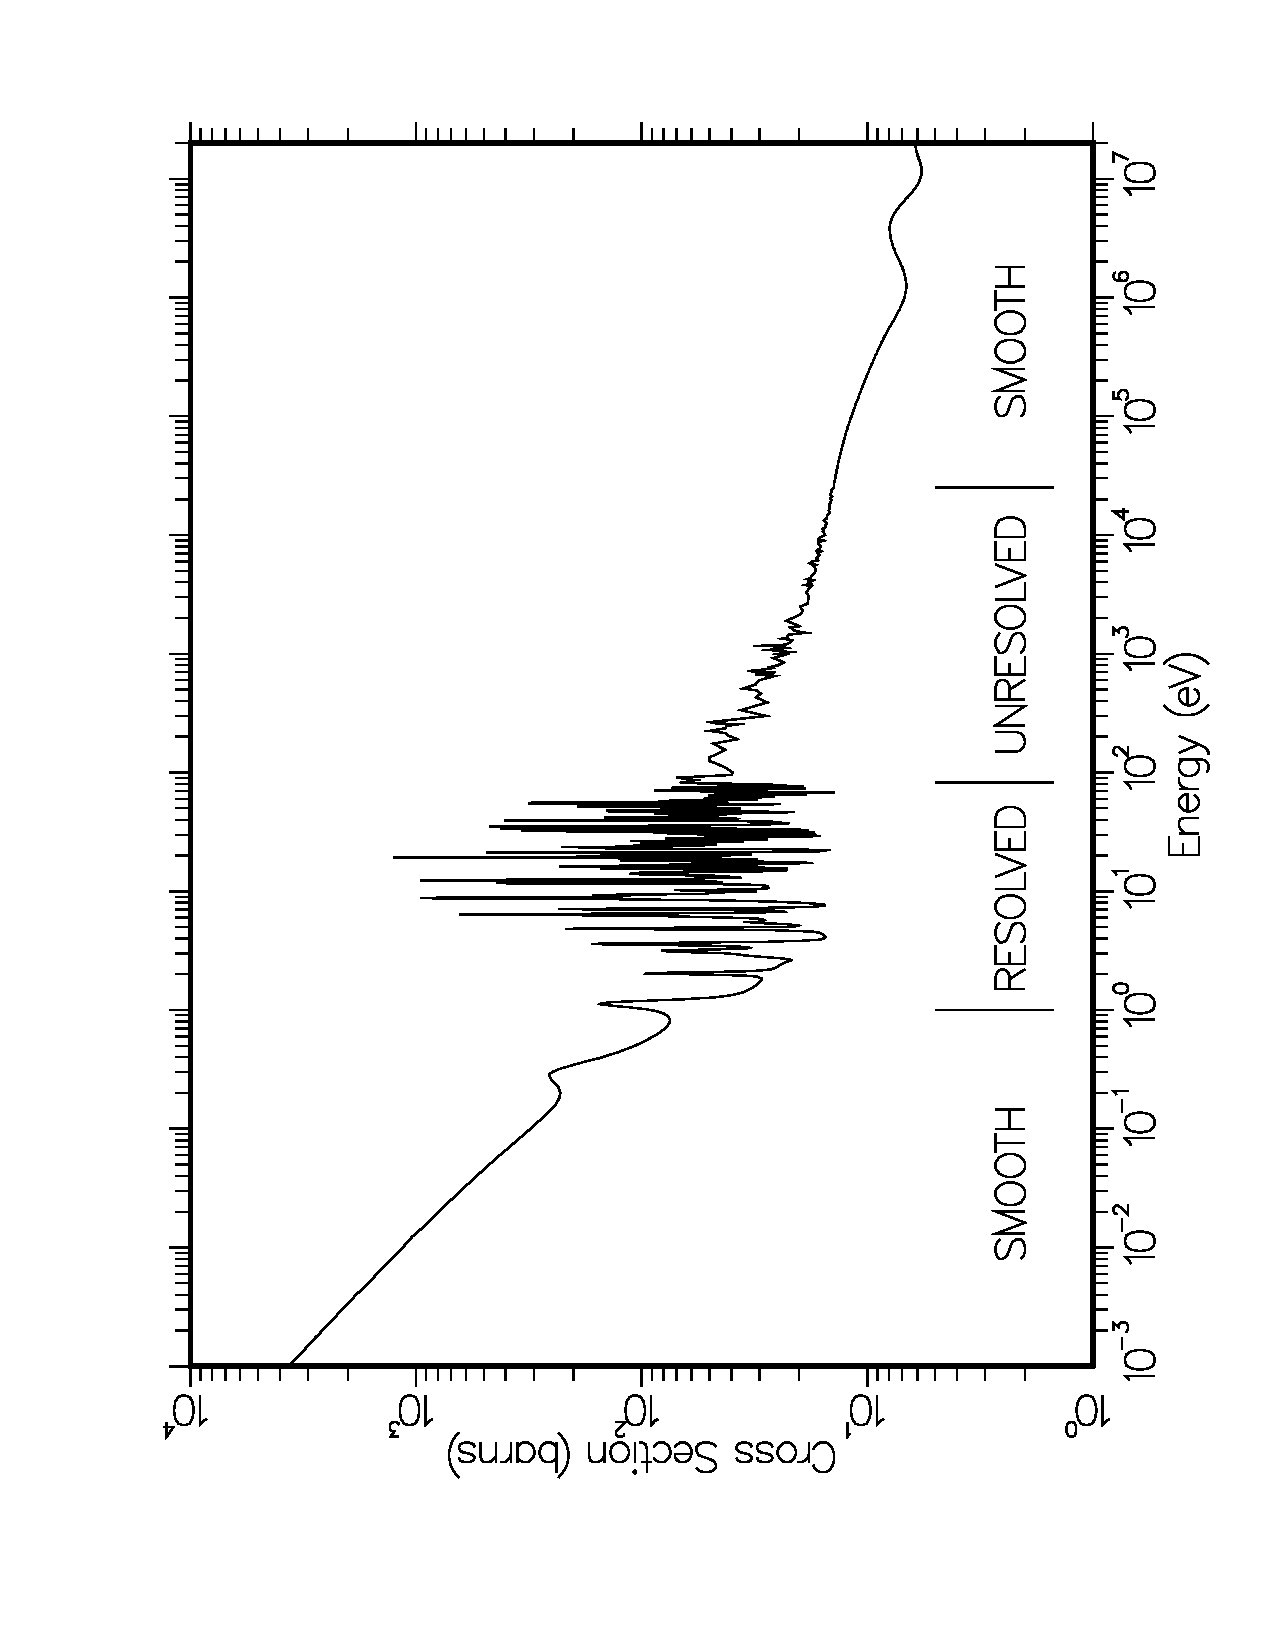
\includegraphics[keepaspectratio,height=4.0in,angle=270]{figs/reconr1ack}
\caption[RECONR reconstructed xs with smooth, RR and URR regions]{A
   typical cross section reconstructed from an ENDF/B
   evaluation using RECONR.  The smooth, resolved, and
   unresolved energy regions use different representations of the
   cross sections.  This is the total cross section for $^{235}$U
   from ENDF/B-V.}
\label{xsfig}
\end{figure}

A typical cross section derived from an ENDF/B evaluation is
shown in Fig.~\ref{xsfig}.  The low-energy cross sections are
``smooth''.\index{smooth cross sections}  They are described
in File 3 (see Section \ref{ssNJOY_ENDF_IO} for a review of
ENDF/B\index{ENDF!ENDF/B} nomenclature) using cross-section values
given on an energy grid with a specified law for
interpolation\index{interpolation} between the points.
In the resolved resonance range\index{resolved resonance range},
resonance parameters are given in File 2, and the cross sections
for resonance reactions have to be obtained by adding the
contributions of all the resonances to ``backgrounds'' from
File 3.  At still higher energies comes the unresolved
region\index{unresolved resonance range} where explicit
resonances are no longer defined.  Instead, the cross section
is computed from statistical distributions of the resonance
parameters given in File 2 and backgrounds from File 3 (or
optionally taken directly from File 3 as for smooth cross
sections).  Finally, at the highest energies, the smooth
File 3 representation is used again.

For light and medium-mass isotopes, the unresolved range is
usually omitted.  For the lightest isotopes, the resolved range
is also omitted, the resonance cross sections being given
directly in the ``smooth'' format.  In addition, several
different resonance representations are supported
(Single-Level Breit-Wigner (SLBW), Multilevel Breit-Wigner (MLBW), Adler-Adler,
Hybrid R-Function (HRF), Reich-Moore (RM), Reich-Moore-Limited (RML),
energy-independent unresolved, and energy-dependent
unresolved).  The Adler-Adler and Hybrid formats are not
being used in modern evaluations.  For an increasing number
of modern evaluations, the low energy ``smooth'' region is
omitted, and the resolved resonance region is extended to the
low energy limit.
\index{Single-Level Breit-Wigner!SLBW}
\index{Multi-Level Breit-Wigner}\index{Multi-Level Breit-Wigner!MLBW}
\index{Reich-Moore}\index{Reich-Moore!RM}
\index{Reich-Moore-Limited}\index{Reich-Moore-Limited!RML}
\index{Adler-Adler}
\index{Hybrid R-Function}\index{Hybrid R-Function!HRF}

RECONR takes these separate representations and produces a simple
cross section versus energy representation like the one shown
in Fig.~\ref{xsfig}.

\subsection{Unionization and Linearization Strategy}
\label{ssRECONR_union}

Several of the cross sections found in ENDF/B evaluations are
summation cross sections\index{summation cross sections}
(for example, total, inelastic, sometimes (n,2n) or fission,
and sometimes charged-particle reactions), and it is important
that each summation cross section be equal to the sum of its parts.
However, if the partial cross sections are represented with
nonlinear interpolation\index{interpolation!nonlinear interpolation}
\index{interpolation} schemes, the sum cannot be represented
by any simple interpolation law.  A typical case is the sum
of elastic scattering (MT=2 interpolated linearly to represent
a constant) and radiative capture (MT=102 interpolated log-log
to represent $1/v$).  The total cross section cannot be
represented accurately by either scheme unless the grid points
are very close together.  This effect leads to significant
balance errors in multigroup transport codes and to splitting
problems in continuous-energy Monte Carlo codes.\index{Monte Carlo}

The use of linear-linear interpolation ({\it i.e.,} $\sigma$ linear
in $E$)\index{interpolation!linear interpolation} can be advantageous in several
ways.  The data can be plotted easily, they can be integrated easily,
cross sections can be Doppler broadened\index{Doppler-broadening}
efficiently (see \hyperlink{sBROADRhy}{BROADR}\index{BROADR}), and,
linear data can be retrieved efficiently in continuous-energy
Monte Carlo codes. \index{Monte Carlo!continuous-energy Monte Carlo}
Therefore, RECONR puts all cross sections on a single unionized
grid suitable for linear interpolation.  As described in more
detail below, RECONR makes one pass through the ENDF/B material
to select the energy grid, and then a second pass to compute
cross sections on this grid.  Each cross section on the
PENDF\index{PENDF} file (except for the summation cross
sections\index{summation cross sections}) is exactly equal
to its ENDF/B value.  The summation cross sections are then
obtained by adding up the partial cross sections at each
grid point.

While RECONR is going through the reactions given in the ENDF/B
evaluation, it also checks the reaction thresholds\index{thresholds}
against the $Q$ value\index{Q-value} and atomic weight
ratio to the neutron $A$ (AWR\index{atomic weight ratio!AWR}
in the file) given for the reaction.  If

\begin{equation}
   {\rm threshold} \ge \frac{A+1}{A}\,Q
\end{equation}

\noindent
is not true, the threshold energy is moved up to satisfy
the condition.  This is usually a small change, often only
in the least significant digit, and is a consequence of
comparing two REAL numbers of finite precision.

If desired, the unionized grid developed from the ENDF/B file can
be supplemented with ``user grid points''\index{user grid} given
in the input data.  The code automatically adds the conventional
thermal point of 0.0253 eV and the 1, 2, and 5 points in each
decade to the grid if they are not already present.  These simple
energy grid points help when comparing materials, and they provide
well-controlled starting points for further subdivision of
the energy grid.

There are special problems with choosing the energy grid in the
unresolved range\index{unresolved resonance range}.  In some cases,
the unresolved cross section is represented using resonance
parameters that are independent of energy.  The cross sections
are not constant, however, but have a shape determined by the
energy variation of neutron wave number, penetrability factors,
and so on.  RECONR handles this case by choosing a set of energies
(about 13 per decade) to be used to calculate the cross sections;
the set of energies gives a reasonable approximation to the result
intended.  For evaluations that use energy-dependent resonance
parameters, it is supposed to be sufficient to compute the
unresolved cross sections at the given energies and to use
interpolation\index{interpolation} on the cross sections to obtain
the appropriate values at other energies.  However, some
evaluations carried over from earlier versions of ENDF/B were not
evaluated using this convention, and cross sections computed
using cross-section interpolation are not sufficiently accurate.
Even some modern evaluations use inadequate energy grids for
the unresolved range.  RECONR detects such cases by looking for
large steps between the points of the given energy grid.  It
then adds additional energy grid points using the same
13-per-decade rule used for energy-independent parameters.
``Large'' is currently defined by \cword{wide} to be a factor
of 1.26.\index{unresolved energy grid}

\subsection{Linearization and Reconstruction Methods}
\label{ssRECONR_linear}

Linearization\index{linearization} (\cword{lunion}) and resonance
reconstruction\index{resonance reconstruction} (\cword{resxs})
both function by inserting new energy grid points between
the points of an original grid using an ``inverted
stack''.\index{inverted stack}  The general concepts involved
are illustrated with a simple example shown in Fig.~\ref{stackfig}.

\begin{figure}[htbp]\centering
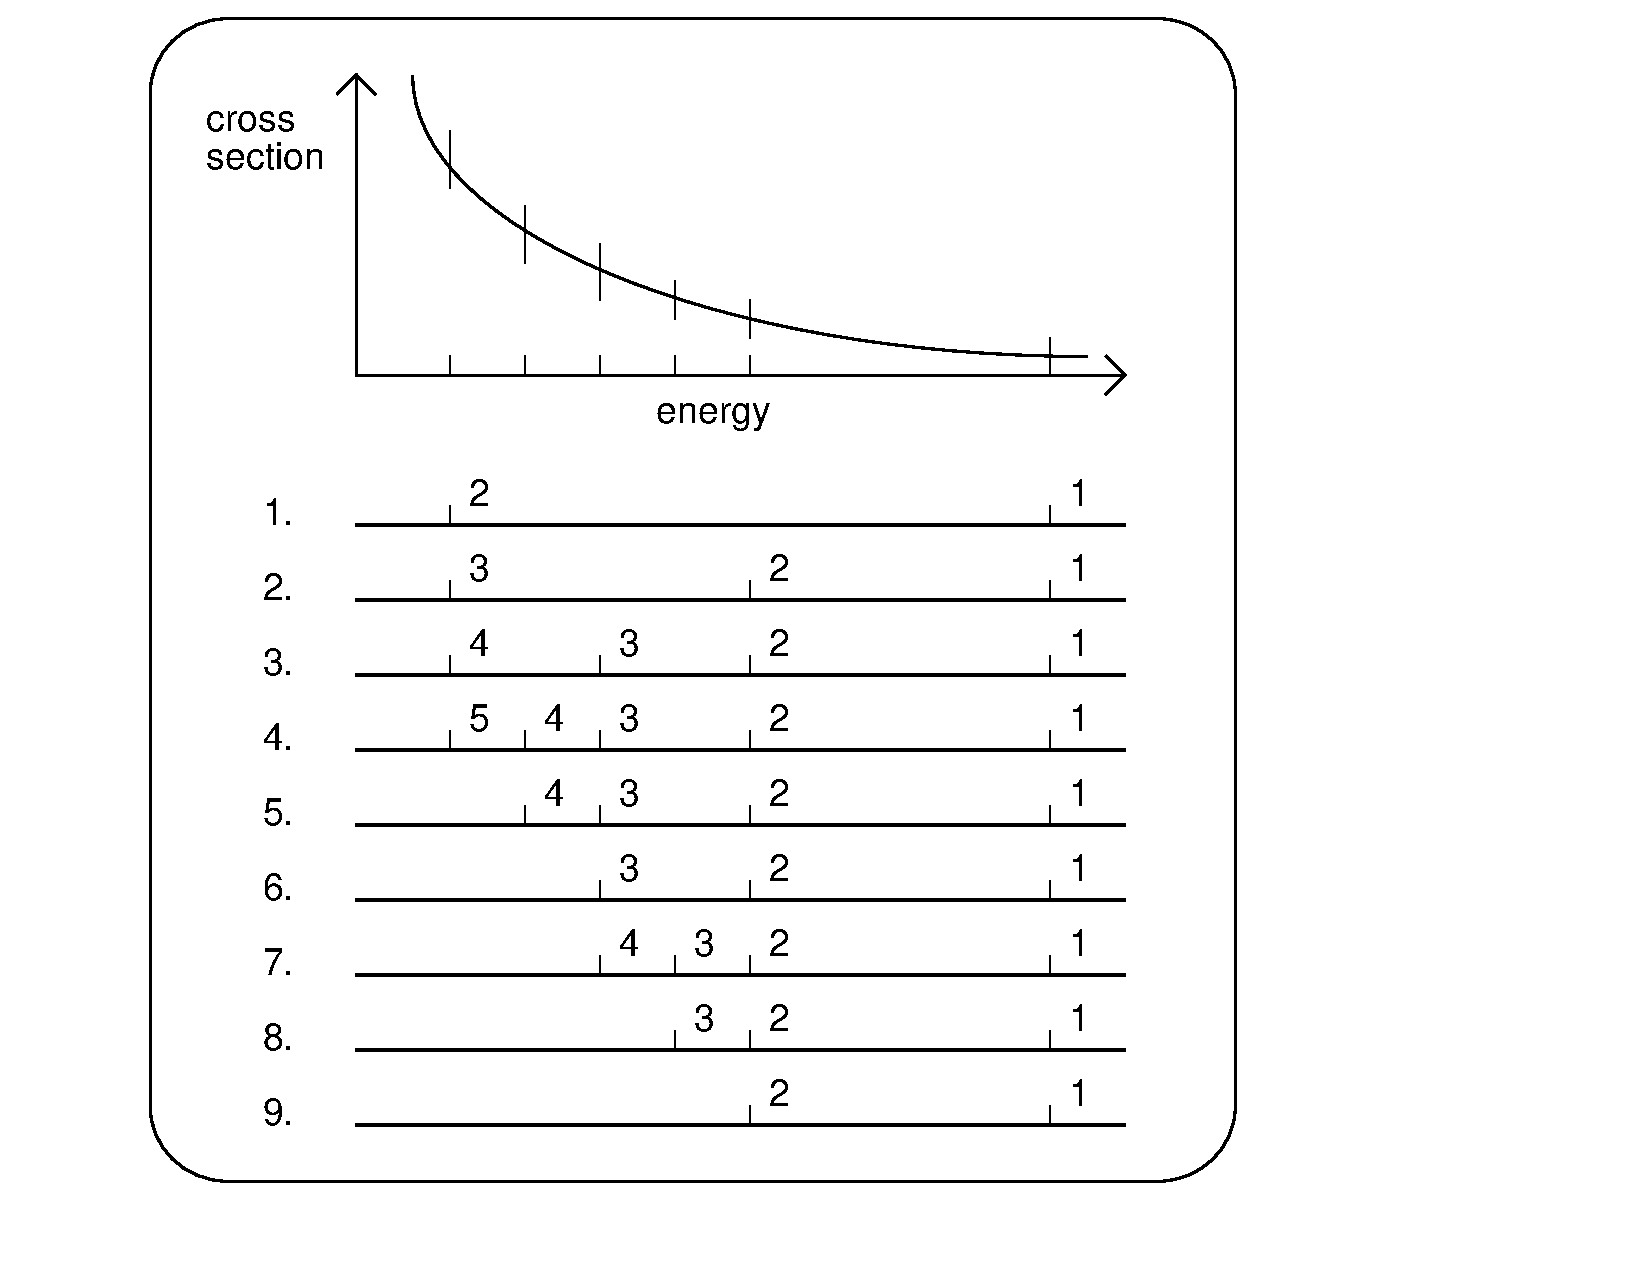
\includegraphics[keepaspectratio, height=5.3in, angle=0]{figs/reconr2ack}
\caption[Inverted stack mesh generation description]{Inverted
     -stack method used in RECONR and several
     other places in NJOY.  Line 1 shows the two initial points
     (the lower energy is higher in the stack).  In line 2, a new
     point has been calculated at the midpoint, but the result was
     not converged, and the new point has been inserted in the
     stack.  In line 3, the midpoint of the top panel has been
     checked again, found to be not converged, and inserted
     into the stack.  The same thing happens in line 4.  In line 5,
     the top panel is found to be converged, and the top point (5)
     has been written out.  The same thing happens in line 6.  In
     line 7, the top panel is tested and found to be not converged.
     The midpoint is added to the stack.  Finally, in line 8, the
     top panel is found to be converged, and the top point is
     written out.  This leaves two points in the stack (see line 9).
     Note that the energy points come off the stack in the desired
     order of increasing energy, and that only one point has to be
     moved up in the stack as each new result is inserted.}
\label{stackfig}
\end{figure}

The stack is first primed with two starting values.  For
linearization, they will be two adjacent points on the original
union grid.  For reconstruction, they will usually be the peaks
and half-height energies of resonances.  The stack is said to be
inverted because the lower energy is at the ``top''
(\cword{I}=2).

This interval or panel is now divided into two parts, and the
cross section computed at the intermediate point is compared to
the result of linear interpolation between the adjacent points.
If the two values do not agree within various criteria, the top
of the stack is moved up one notch (\cword{I}=3), and the new
value is inserted (\cword{I}=2).  The code then repeats the
checking process for the new (smaller) interval at the top of the
stack.  The top of the stack rises until convergence is achieved
for the top interval.  The top energy and cross section are then
saved on a scratch file, the stack index is decremented, and the
checks are repeated.  This process is continued with the top of
the stack rising and falling in response to the complexity of the
cross section until the entire panel $\Delta E$ has been
converged (\cword{I}=1).  The stack is then reprimed with the
bounds of the next panel.  The process continues until the entire
energy range for linearization or reconstruction has been
processed.

This stack logic enables a panel to be subdivided into parts as
small as $\Delta E / 2^n$ where $n$ is the stack size, and several
different cross sections (elastic, capture, fission) can easily
be stored in arrays of this size.

The convergence criterion used for linearization is that the
linearized cross section at the intermediate point is within the
fractional tolerance \cword{err} (or a small absolute value
\cword{errlim}) of the actual cross section specified by the
ENDF law. More complicated criteria are used for resonance
reconstruction.

There are two basic problems that arise if a simple fractional
tolerance test is used to control resonance reconstruction.
First, as points are added to the energy grid, adjacent energy
values may become so close that they will be rounded to the same
number when a formatted output file is produced.  There can be
serious problems if the code continues to add grid points after
this limit is reached.  Through the use of dynamic format
reconstruction, the energy resolution available for formatted
NJOY output (which use ENDF 11-character fields) is 7
significant figures\index{significant figures} (that is,
$\pm 1.234567\pm n$) rather than the usual 5 or 6 (see Section
\ref{ssNJOY_ENDF_IO}).  For NJOY2016, the Fortran-90 ``kind'' parameter is
used to assure sufficient precision for this.  Even this
seven significant figure format is sometimes insufficient for
very narrow resonances.  If necessary, NJOY can go to nine
significant figures by using a Fortran ``F'' format,
{\it e.g.,} $\pm 1234.56789$.

Significant-figure control is implemented as follows:  each
intermediate energy is first truncated to 7 significant
figures before the corresponding cross sections are computed.
If the resulting number is equal to either of the adjacent
values and convergence has not been obtained, subdivision
continues using energies truncated to 9 significant figures.
If an energy on this finer grid is equal to either of the
adjacent values, the interval is declared to be converged
even though convergence has not been achieved.  Thus, no
identical energies are produced, but an unpredictable but
very small loss in accuracy results.

The second basic problem alluded to above is that a very large
number of resonance grid points arise from straightforward
linear reconstruction of the resonance cross section of some
isotopes.  Many of these points come from narrow, weak,
high-energy resonances, which do not need to be treated
accurately in many applications.  As an example, the capture and
fission resonance integrals important for thermal reactors must
be computed with a $1/E$ flux weighting.  If the resonance
reconstruction tolerance is set high (say 1\%) to reduce the cost
of processing, the resonance integrals will be computed to only
1\% accuracy.  However, if the reconstruction tolerance were set
to a smaller value, like 0.1\%, and if the high-energy resonances
(whose importance is reduced by the $1/E$ weight and the $1/v$
trend of the capture and fission cross sections) were treated
with less accuracy than the low-energy resonances, then it is
likely that one could achieve an accuracy much better than 1\%
with an overall reduction in the number of points (hence computing
cost).  Since $1/E$ weighting is not realistic in all applications
(for example, in fast reactors), user control of this
``thinning'' operation must be provided.

Based on these arguments, the following approach was chosen to
control the problem of very large files.  First, panels are
subdivided until the elastic, capture, and fission cross sections
are converged to within \cword{errmax}, where \cword{errmax}
$\ge$ \cword{err}.  These two tolerances are normally chosen to
form a reasonable band, such as 1\% and 0.1\%, to ensure that
all resonances are treated at least roughly (for example, for
plotting).  If the resonance integral ($1/E$ weight) in some panel
is large, the panel is further subdivided to achieve an accuracy
of \cword{err} (say 0.1\%).  However, if the contribution to the
resonance integral from any one interval gets small, the interval
will be declared converged, and the local value of the cross
section will end up with some intermediate accuracy.  The
contribution to the error in the resonance integral should be
less than $0.5{\times}\Delta\sigma{\times}\Delta E$.  This value
is added into an accumulating estimate of the error, and a count
of panels truncated by the resonance integral check is
incremented.
\index{integral thinning}
\index{resonance integral check}

The problem with this test is that RECONR does not know the value
of the resonance integral in advance, so the tolerance parameter
\cword{errint} is not the actual allowed fractional error in the
integral.  Instead, it is more like the resonance integral error
per grid point (barns/point).  Thus, a choice of
\cword{errint=err/10000} with \cword{err}=0.001 would limit the
integral error to about 0.001 barn if 10000 points resulted from
reconstruction.  Since important resonance integrals vary from a
few barns to a few hundred barns, this is a reasonable choice.
The integral check can be suppressed by setting \cword{errint}
very small or \cword{errmax=err}.

When resonance reconstruction is complete, RECONR provides a
summary of the possible resonance integral error due to the
integral check over several coarse energy bands.  An example
from ENDF/B-VII.0 $^{235}$U follows:

\newpage
\small
\begin{ccode}

               estimated maximum error due to
               resonance integral check (errmax,errint)

    upper      elastic   percent   capture   percent   fission   percent
    energy     integral   error    integral   error    integral   error
  1.00E-05
  1.00E-04     3.50E+01   0.000    8.15E+03   0.000    4.29E+04   0.000
  1.00E-03     3.50E+01   0.000    2.57E+03   0.000    1.36E+04   0.000
  1.00E-02     3.50E+01   0.000    8.02E+02   0.000    4.24E+03   0.000
  1.00E-01     3.46E+01   0.000    2.15E+02   0.000    1.26E+03   0.000
  1.00E+00     3.25E+01   0.000    6.03E+01   0.000    3.26E+02   0.000
  2.00E+00     8.95E+00   0.000    7.31E+00   0.000    2.62E+01   0.000
  5.00E+00     1.08E+01   0.000    1.25E+01   0.000    1.56E+01   0.000
  1.00E+01     7.75E+00   0.000    2.40E+01   0.000    3.52E+01   0.000
  2.00E+01     8.18E+00   0.000    2.92E+01   0.000    3.31E+01   0.000
  5.00E+01     1.07E+01   0.000    2.57E+01   0.000    3.83E+01   0.000
  1.00E+02     8.30E+00   0.000    1.07E+01   0.000    2.34E+01   0.000
  2.00E+02     8.04E+00   0.000    8.17E+00   0.000    1.42E+01   0.000
  5.00E+02     1.10E+01   0.001    6.81E+00   0.008    1.51E+01   0.004
  1.00E+03     8.28E+00   0.008    3.44E+00   0.080    7.62E+00   0.038
  2.00E+03     8.27E+00   0.033    2.54E+00   0.261    5.06E+00   0.185

 points added by resonance reconstruction    =  232418
 points affected by resonance integral check =   80445
 final number of resonance points            =  242170
 number of points in final unionized grid    =  242600

\end{ccode}
\normalsize

\noindent
The parameters \cword{errmax} and \cword{errint}, taken together,
should be considered as adjustment ``knobs'' that can increase or
decrease the errors in the ``res-int'' columns to get an appropriate
balance between accuracy and economy for a particular application.
The error from significant figure reduction provided by earlier
versions of NJOY is no longer needed.

For energies in the thermal range (energies less than
\cword{trange}=0.5 eV), the user's reconstruction
tolerance\index{thermal reconstruction tolerance} is
divided by a factor of 5 in order to give better results for
several important thermal integrals, especially after Doppler
broadening, and to make the 0.0253 eV cross section behave
well under Doppler broadening.

\subsection{Resonance Representations}
\label{ssRECONR_resrep}

RECONR uses the resonance formulas as implemented in the original
RESEND code\cite{RESEND}\index{RESEND} with several changes:  a
more efficient calculation of MLBW cross sections \index{Multi-Level
Breit-Wigner!MLBW} developed by C. R. Lubitz\index{Lubitz} of the
Knolls Atomic Power Laboratory (KAPL)\index{Knolls Atomic Power
Laboratory!KAPL} and coded by P. Rose \index{Rose} of the National
Nuclear Data Center (NNDC)\index{National Nuclear Data Center!NNDC}
\index{NNDC|see{National Nuclear Data Center}} at
the Brookhaven National Laboratory (BNL)\index{Brookhaven National
Laboratory!BNL}, the addition of competitive widths\index{competitive width}
introduced for ENDF/B-V, a $\psi\chi$ Doppler-broadening\index{$\psi\chi$
broadening} calculation for SLBW\index{Single-Level Breit-Wigner!SLBW} and
Adler-Adler \index{Adler-Adler} resonance shapes, and a capability to
process either the multi-level multi-channel R-matrix
Reich-Moore\index{Reich-Moore!RM} parameters or
the multi-level single-channel Hybrid R-Function\index{Hybrid R-Function!HRF}
parameters based on the work of
M. Bhat\index{Bhat} and C. Dunford\index{Dunford} of the NNDC,
an implementation of the GH method\index{Multi-Level Breit-Wigner!GH MLBW
method} for MLBW resonances, which allows psi-chi broadening, and a capability
to process the new RML\index{Reich-Moore-Limited!RML}
parameters, including resolved resonance energy region angular distributions.
\index{resonance angular distributions}

Expanded discussions of the following formulas can be found in the
ENDF-6 format manual\cite{ENDF102}.\index{ENDF!ENDF format!ENDF-6 format}

\paragraph{Single-Level Breit-Wigner Representation (SLBW)}
\index{Single-Level Breit-Wigner}
The subroutine that computes Single-Level Breit-Wigner cross
sections\index{Single-Level Breit-Wigner!SLBW}
(\cword{csslbw})\index{csslbw@{\ty csslbw}} uses
\begin{eqnarray}
  \sigma_n&=&\sigma_p\nonumber\\
      & &+\sum_{\ell}\sum_r\sigma_{mr}
    \Bigl\lbrace \Bigl[ \cos 2\phi_\ell - (1-{{\Gamma_{nr}}
    \over {\Gamma_r}}) \Bigr] \,\psi(\theta,x)\nonumber\\
    & &+\sin 2\phi_\ell \,\chi(\theta,x) \Bigr\rbrace\,\,,\\
  \sigma_f&=&\sum_{\ell}\sum_r \sigma_{mr} {{\Gamma_{fr}}
     \over{\Gamma_r}}\,\psi(\theta,x)\,\,,\\
  \sigma_\gamma&=&\sum_{\ell}\sum_r\sigma_{mr} {{\Gamma_{\gamma r}}
     \over {\Gamma_r}} \,\psi(\theta,x)\,\,,\;\hbox{and}\\
  \sigma_p&=&\sum_\ell {{4\pi}\over{k^2}}(2\ell+1)\sin^2
     \theta_\ell \,\,,
\end{eqnarray}
where $\sigma_n$, $\sigma_f$, $\sigma_\gamma$, and $\sigma_p$ are
the neutron (elastic), fission, radiative capture, and potential
scattering components of the cross section arising from the given
resonances.  There can be ``background'' cross sections in File 3
that must be added to these values to account for competitive
reactions such as inelastic scattering or to correct for the
inadequacies of the single-level representation with regard to
multilevel effects or missed resonances.  The sums extend over
all the $\ell$ values and all the resolved resonances $r$ with a
particular value of $\ell$.  Each resonance is characterized by
its total, neutron, fission, and capture widths ($\Gamma,
\Gamma_n, \Gamma_f, \Gamma_\gamma$), by its $J$ value (AJ in the
file), and by its maximum value (\cword{smax}$=\sigma_{mr} /
\Gamma_r$ in the code)
\begin{equation}
   \sigma_{mr} = {\frac{4\pi}{k^2}}\,g_J \,{\frac{\Gamma_{nr}}
      {\Gamma_r}} \,\,,
\end{equation}
where $g_J$ is the spin statistical factor
\begin{equation}
   g_J={\frac{2J+1}{4I+2}}\,\,,
\end{equation}
and $I$ is the total spin (SPI) given in File 2, and $k$ is the
neutron wave number, which depends on incident energy $E$ and the
atomic weight ratio to the neutron for the isotope $A$ (AWRI in
the file), as follows:
\begin{equation}
   k=(2.196771{\times}10^{-3}){\frac{A}{A+1}}\sqrt{E}\,\,.
\end{equation}
There are two different characteristic lengths that appear in the
ENDF resonance formulas:  first, there is the ``scattering
radius''\index{scattering radius} $\hat a$, which is given
directly in File 2 as AP; and second, there is the ``channel
radius''\index{channel radius} $a$, which is given by
\begin{equation}
   a=0.123\,A^{1/3}+0.08\,\,.
\end{equation}
If the File 2 parameter NAPS is equal to one, $a$ is set equal to
$\hat a$ in calculating penetrabilities and shift factors (see
below).  The ENDF-6 option to enter an energy-dependent
scattering radius is not supported.  The neutron width in the
equations for the SLBW cross sections is energy dependent due to
the penetration factors $P_\ell$;  that is,
\index{penetrabilities}
\begin{equation}
   \Gamma_{nr}(E)={\frac{P_\ell(E)\,\Gamma_{nr}}{P_\ell(|E_r|)}}\,\,,
\end{equation}
where
\begin{eqnarray}
  P_0&=&\rho\,\,,\\
  P_1&=&{\frac{\rho^3}{1+\rho^2}}\,\,,\\
  P_2&=&{\frac{\rho^5}{9+3\rho^2+\rho^4}}\,\,,\\
  P_3&=&{\frac{\rho^7}{225+45\rho^2+6\rho^4+\rho^6}}\,\,,
              \;\hbox{and}\\
  P_4&=&{\frac{\rho^9}{11025+1575\rho^2+135\rho^4+10\rho^6+\rho^8}}\,\,,
\end{eqnarray}
where $E_r$ is the resonance energy and $\rho{=}ka$ depends on
the channel radius or the scattering radius as specified by NAPS.
The phase shifts are given by
\index{phase shifts}
\begin{eqnarray}
  \phi_0&=&\hat\rho\,\,,\\
  \phi_1&=&\hat\rho - \tan^{-1}\hat\rho \,\,,\\
  \phi_2&=&\hat\rho - \tan^{-1}{\frac{3\hat\rho}
    {3-\hat\rho^2}} \,\,,\\
  \phi_3&=&\hat\rho - \tan^{-1}{\frac{15\hat\rho-\hat\rho^3}
    {15-6\hat\rho^2}} \,\,,\;\hbox{and}\\
  \phi_4&=&\hat\rho - \tan^{-1}{\frac{105\hat\rho-10\hat\rho^3}
    {105-45\hat\rho^2+\hat\rho^4}}\,\,,
\end{eqnarray}
where $\hat\rho{=}k\hat a$ depends on the scattering radius.  The
final components of the cross section are the actual line shape
functions $\psi$ and $\chi$.  At zero temperature,
\begin{eqnarray}
  \psi&=&{\frac{1}{1+x^2}}\,\,,\\
  \chi&=&{\frac{x}{1+x^2}}\,\,,\\
  x&=&{\frac{2(E-E'_r)}{\Gamma_r}}\,\,,
\end{eqnarray}
and
\begin{equation}
   E'_r=E_r+{\frac{S_\ell(|E_r|)-S_\ell(E)}
    {2(P_\ell(|E_r|)}}\,\Gamma_{nr}(|E_r|)\,\,,
\label{r24}
\end{equation}
in terms of the shift factors
\index{resonance shift factors}
\begin{eqnarray}
  S_0&=&0\,\,,\\
  S_1&=&-{\frac{1}{1+\rho^2}}\,\,,\\
  S_2&=&-{\frac{18+3\rho^2}{9+3\rho^2+\rho^4}} \,\,,\\
  S_3&=&-{\frac{675+90\rho^2+6\rho^4}{225+45\rho^2+6\rho^4+\rho^6}}\,\,,
         \;\hbox{and}\\
  S_4&=&-{\frac{44100+4725\rho^2+270\rho^4+10\rho^6}
           {11025+1575\rho^2+135\rho^4+10\rho^6+\rho^8}}\,\,.
\end{eqnarray}
To go to higher temperatures, define
\begin{equation}
   \theta={\frac{\Gamma_r}
    {\displaystyle\sqrt{{\frac{4kTE}{A}}}}}\,\,,
\end{equation}
where $k$ is the Boltzmann constant\index{Boltzmann constant}
and $T$ is the absolute temperature.
\index{$\psi\chi$ broadening}
The line shapes $\psi$ and $\chi$ are now given by
\begin{equation}
   \psi={\frac{\sqrt{\pi}}{2}}\,\theta \,{\rm Re} W\bigl(
    {\frac{\theta x}{2}},{{\theta}\over 2}\bigr)\,\,,
\end{equation}
and
\begin{equation}
   \chi={{\sqrt{\pi}}\over 2} \,\theta \,{\rm Im}W\bigl(
    {{\theta x}\over 2},{{\theta}\over 2}\bigr)\,\,,
\end{equation}
in terms of the complex probability function (see \cword{quickw},
\cword{wtab}, and \cword{w}, which came from the MC$^2$ code\cite{MC2})
\begin{equation}
   W(x,y)={\rm e}^{-z^2}\,{\rm erfc}(-iz)
    ={\frac{i}{\pi}}\int_{-\infty}^\infty
    {{{\rm e}^{-t^2}}\over{z-t}}\,dt\,\,,
\end{equation}
where $z{=}x{+}iy$.  The $\psi\chi$ method is not as accurate as
kernel broadening\index{kernel broadening} (see
\hyperlink{sBROADRhy}{BROADR}\index{BROADR})
because the backgrounds (which are sometimes quite complex) are not
broadened, and terms important for energies less than about $16kT/A$
are neglected; however, the $\psi\chi$ method is less expensive than
\hyperlink{sBROADRhy}{BROADR}.  Previous versions of
RECONR included $\psi\chi$ broadening
\index{$\psi\chi$ broadening} for the SLBW
\index{Single-Level Breit-Wigner!SLBW} and Adler-Adler\index{Adler-Adler}
representations only.  This version also allows the method to be used
for MLBW\index{Multi-Level Breit-Wigner!MLBW} cases.  The
SLBW approach can produce negative elastic
cross sections.\index{negative cross sections} If found, they are
set to a small positive value, and a count is accumulated for a
diagnostic in the listing file.

\paragraph{Multilevel Breit-Wigner Representation (MLBW)}
\index{Multi-Level Breit-Wigner}
The Lubitz-Rose method used for calculating Multi-Level
Breit-Wigner cross sections (\cword{csmlbw}) is formulated as
follows:
\index{Lubitz-Rose method}
\index{Multi-Level Breit-Wigner!MLBW}
\index{csmlbw@{\ty csmlbw}}
\begin{equation}
  \sigma_n(E)={\frac{\pi}{k^2}}
    \sum_\ell \sum_{s=|I-\frac{1}{2}|}^{I+\frac{1}{2}}
    \sum_{J=|l-s|}^{l+s} g_J\,|1-U_{nn}^{\ell sJ}(E)|^2\,\,,
\end{equation}

\noindent with

\begin{equation}
  U_{nn}^{\ell J}(E)={\rm e}^{2i\phi_\ell}-
    \sum_r {\frac{i\Gamma_{nr}}
    {E'_r-E-i\Gamma_r/2}}\,\,,
\end{equation}

\noindent
where the other symbols are the same as those used above.
Expanding the complex operations gives

\begin{eqnarray}
  \sigma_{n}(E)&=&{\frac{\pi}{k^2}}
    \sum_\ell \sum_{s=|I-\frac{1}{2}|}^{I+\frac{1}{2}}
    \sum_{J=|l-s|}^{l+s} g_J
     \biggl\lbrace \Bigl( 1-\cos 2\phi_\ell -
    \sum_r {{\Gamma_{nr}}\over{\Gamma_r}}
    {2\over{1+x_r^2}} \Bigr)^2\nonumber\\
   &+&\Bigl(\sin 2\phi_\ell
    +\sum_r {{\Gamma_{nr}}\over{\Gamma_r}}
    {\frac{2x_r}{1+x_r^2}} \Bigr)^2 \biggr\rbrace \,\,,
\end{eqnarray}

\noindent
where the sums over $r$ are limited to resonances in spin
sequence $\ell$ that have the specified value of $s$ and $J$.
Unfortunately, the $s$ dependence of $\Gamma$ is not known.
The file contains only $\Gamma_J{=}\Gamma_{s_1J}{+}\Gamma_{s_2J}$.
It is assumed that the $\Gamma_J$ can be used for one of the
two values of $s$, and zero is used for the other.  Of course,
it is important to include both channel-spin terms in the
potential scattering.  Therefore, the equation is written in
the following form:
\index{channel spin}
\index{potential scattering}

\begin{eqnarray}
  \sigma_{n}(E)&=&{\frac{\pi}{k^2}}
    \sum_\ell \biggl[
    \sum_J g_J \biggl\lbrace \Bigl( 1-\cos 2\phi_\ell -
    \sum_r {{\Gamma_{nr}}\over{\Gamma_r}}
    {2\over{1+x_r^2}} \Bigr)^2\nonumber\\
   &+&\Bigl(\sin 2\phi_\ell
    +\sum_r {{\Gamma_{nr}}\over{\Gamma_r}}
    {\frac{2x_r}{1+x_r^2}} \Bigr)^2 \biggr\rbrace
    +2D_\ell(1-\cos 2\phi_\ell) \biggr] \,\,,
\end{eqnarray}

\noindent where the summation over $J$ now runs from

\begin{equation}
   ||I-\ell|-\frac{1}{2}| \rightarrow I+\ell+\frac{1}{2} \,\,,
\end{equation}

\noindent and $D_\ell$ gives the additional contribution to the
statistical weight resulting from duplicate $J$ values not
included in the new $J$ sum; namely,
\index{J values@{J values!duplicate $J$ values}}

\begin{eqnarray}
   D_\ell&=&
    \sum_{s=|I-\frac{1}{2}|}^{I+\frac{1}{2}}
    \sum_{J=|l-s|}^{l+s} g_J \;
    -\sum_{J=||I-\ell|-\frac{1}{2}|}^{I+\ell+\frac{1}{2}} g_J \\
    &=&(2\ell+1) \;
    -\sum_{J=||I-\ell|-\frac{1}{2}|}^{I+\ell+\frac{1}{2}} g_J\,\,.
\label{missing}
\end{eqnarray}

\noindent
A case where this correction would appear is the $\ell{=}1$ term
for a spin-1 nuclide.  There will be 5 $J$ values:  1/2, 3/2, and
5/2 for channel spin 3/2; and 1/2 and 3/2 for channel spin 1/2.
All five contribute to the potential scattering, but the file
will only include resonances for the first three.

The fission and capture cross sections are the same as for the
single-level option.  The $\psi\chi$ Doppler-broadening cannot be
used with this formulation of the MLBW representation.
\index{$\psi\chi$ broadening}\index{Multi-Level Breit-Wigner!MLBW}

However, there is an alternate representation available that
does support $\psi\chi$ broadening:
\begin{eqnarray}
  \sigma_n&=&\sigma_p\nonumber\\
      & &+\sum_{\ell}\sum_r\sigma_{mr}
    \Bigl\lbrace \Bigl[ \cos 2\phi_\ell - (1-{{\Gamma_{nr}}
    \over {\Gamma_r}})+\frac{G_{r\ell}}{\Gamma_{nr}} \Bigr]
      \,\psi(\theta,x)\nonumber\\
    & &+(\sin 2\phi_\ell +\frac{H_{r\ell}}{\Gamma_{nr}})
      \,\chi(\theta,x) \Bigr\rbrace\,\,,
\end{eqnarray}
where
\begin{equation}
   G_{r\ell}=\frac{1}{2}
    \sum_{\stackrel{\displaystyle r'\ne r}
    {\displaystyle J_{r'}\ne J_r}}
    \Gamma_{nr}\Gamma_{nr'}\frac{\Gamma_r+\Gamma_{r'}}
      {(E_r-E_{r'})^2+(\Gamma_r+\Gamma_{r'})^2/4} \,,
\end{equation}
and
\begin{equation}
   H_{r\ell}=\sum_{\stackrel{\displaystyle r'\ne r}
    {\displaystyle J_{r'}\ne J_r}}
    \Gamma_{nr}\Gamma_{nr'}\frac{E_r-E{r'}}
      {(E_r-E_{r'})^2+(\Gamma_r+\Gamma_{r'})^2/4} \,.
\end{equation}
Nominally, this method is slower than the previous one because
it contains a double sum over resonances at each energy.  However,
it turns out that G and H are slowly varying functions of energy,
and the calculation can be accelerated by computing them at just
a subset of the energies and getting intermediate values by
interpolation.  It is important to use a large number of $r'$
values on each side of $r$.  The GH MLBW method is implemented
in \cword{csmlbw2}.
\index{Multi-Level Breit-Wigner!GH MLBW method}
\index{csmlbw2@{\ty csmlbw2}}

\paragraph{Adler-Adler Representation (Adler-Adler)}
\index{Adler-Adler}
The multilevel Adler-Adler representation
 (\cword{csaa})\index{csaa@{\ty csaa}}
is defined for $\ell{=}0$ only.  It is useful for fissionable
materials.  The total cross sections are given by

\begin{eqnarray}
  \sigma_t(E)&=&{\frac{4\pi}{k^2}}\sin^2\phi_0\nonumber\\
  &+&{\frac{\pi\sqrt{E}}{k^2}} \biggl\lbrace
    \sum_r {\frac{1}{\nu_r}} \biggl[(G_r\cos 2\phi_0
    +H_r\sin 2\phi_0 ) \,\psi(\theta,x)\nonumber\\
  &+&(H_r\cos 2\phi_0 - G_r\sin 2\phi_0) \,\chi(\theta,x)
    \biggr]\nonumber\\
  &+&A_1+{\frac{A_2}{E}}+{\frac{A_3}{E^2}}
    +{\frac{A_4}{E^3}}+B_1E+B_2 E^2 \biggr\rbrace \,\,,
\end{eqnarray}

\noindent where

\begin{equation}
  x={\frac{\mu_r-E}{\nu_r}}\,\,,
\end{equation}
\vspace{0.5 pt}

\noindent and where $\nu_r$ is the resonance half-width (corresponds
to $\Gamma /2$ in the Breit-Wigner notation), $\mu_r$ is the
resonance energy, $G_r$ is the symmetric total parameter,
$H_r$ is the asymmetric total parameter, and the $A_i$ and
$B_i$ are coefficients of the total background correction.

The fission and capture cross section both use the form

\begin{eqnarray}
  \sigma_x(E)&=&{\frac{\pi\sqrt{E}}{k^2}}
    \biggl\lbrace \sum_r {\frac{1}{\nu_r}}
    \left[G_r\psi(\theta,x)+H_r\chi(\theta,x)\right]\nonumber\\
  &+&A_1+{\frac{A_2}{E}}+{\frac{A_3}{E^2}}
    +{\frac{A_4}{E^4}}+B_1E+B_2E^2 \biggr\rbrace \,\,,
\end{eqnarray}

\noindent where the values of $G$, $H$, $A_i$, and $B_i$
appropriate for the desired reaction are used.

Doppler-broadening\index{$\psi\chi$ broadening} can be applied
as for the SLBW\index{Single-Level Breit-Wigner!SLBW} case, except note
that $\Gamma_r$ in Eq.~\ref{r24} must be replaced with $2\nu_r$.
Doppler-broadened Adler-Adler cross sections are more accurate
than SLBW cross sections because the background is smoother.
However, cross sections below about $16kT/A$ will still be
inaccurate.  The Adler-Adler method is not used in modern
evaluations.

\paragraph{Reich-Moore Representation (RM)}\index{Reich-Moore}
The Reich-Moore representation\index{Reich-Moore!RM}
as implemented in subroutine \cword{csrmat}\index{csrmat@{\ty csrmat}}
is a multi-level formulation with two fission channels; hence,
it is useful for both structural and fissionable materials.
The cross sections are given by

\begin{eqnarray}
    \sigma_t&=&{\frac{2\pi}{k^2}}\sum_\ell\sum_J
        g_J \Bigl\{ \bigl( 1-{\rm Re}\,U_{nm}^{\ell J}
        \bigr) + 2d_{\ell J}\bigl[1-\cos(2\phi_\ell)
        \bigr]\Bigr\} \,\,,\\
    \sigma_n&=&{\frac{\pi}{k^2}}\sum_\ell\sum_J
      g_J \Bigl\{ | 1-U_{nn}^{\ell J} |^2
         + 2d_{\ell J}\bigl[1-\cos(2\phi_\ell) \Bigr]
        \,\,,\\
    \sigma_f&=&{\frac{4\pi}{k^2}}\sum_\ell\sum_J
      g_J \sum_c |{\cal I}_{nc}^{\ell J} |^2 \,\,,\;\hbox{and}\\
  \sigma_\gamma&=&\sigma_t-\sigma_n-\sigma_f \,\,,
\end{eqnarray}

\noindent where ${\cal I}_{nc}$ is an element of the inverse of the
complex R-matrix\index{R-matrix} and

\begin{equation}
  U_{nn}^{\ell J}={\rm e}^{2i\phi_\ell}\,
    \Bigl[ \,2{\cal I}_{nn}-1\, \Bigr] \,\,.
\label{ufun}
\end{equation}

\noindent The elements of the R-matrix are given by

\begin{equation}
  R_{nc}^{\ell J}=\delta_{nc}
    -{\frac{i}{2}}\sum_r {{\Gamma_{nr}^{1/2}\Gamma_{cr}^{1/2}}
    \over{E_r-E-{\frac{i}{2}}\Gamma_{\gamma r}}}\,\,.
\end{equation}
\vspace{0.5 pt}

\noindent In these equations, ``c'' stands for the fission channel, ``r''
indexes the resonances belonging to spin sequence ($\ell,J$), and
the other symbols have the same meanings as for SLBW or MLBW.  Of
course, when fission is not present, $\sigma_f$ can be ignored.
The R-matrix reduces to an R-function\index{R-function}, and
the matrix inversion normally required to get ${\cal I}_{nn}$
reduces to a simple inversion of a complex number.

As in the MLBW\index{Multi-Level Breit-Wigner!MLBW} case, the
summation over $J$ runs from

\begin{equation}
   ||I-\ell|-\frac{1}{2}| \rightarrow I+\ell+\frac{1}{2} \,\,.
\end{equation}

\noindent The term $d_{\ell J}$ in the expressions for the total and
elastic cross sections is used to account for the possibility
of an additional contribution to the potential scattering
cross section from the second channel spin.  It is unity
if there is a second $J$ value equal to $J$, and zero otherwise.
This is just a slightly different approach for making the
correction discussed in connection with Eq.~(\ref{missing}).
Returning to the $I{=}1$, $\ell{=}1$ example given above,
$d$ will be one for $J{=}1/2$ and $J{=}3/2$, and it will
be zero for $J{=}5/2$.

ENDF-6 format RM evaluations can contain a parameter
LAD that indicates that these parameters can be used to compute an
angular distribution\index{resonance angular distributions}
for elastic scattering if desired (an approximate angular
distribution is still given in File 4 for these cases).  The
current version of RECONR has such a capability, and it can
be used with RM\index{Reich-Moore!RM} evaluations.  Because of channel-spin
issues, it works best with RML\index{Reich-Moore-Limited!RML} evaluations.
See below for a discusion of angular distributions.

\paragraph{Hybrid R-Function Representation (HRF)}\index{Hybrid R-Function}
The Hybrid R-Function representation\index{Hybrid R-Function!HRF} treats
elastic scattering as a multi-level
cross section using formulas similar to those given above
for the Reich-Moore\index{Reich-Moore!RM} format
in the case where fission is absent.  The other reactions are
treated with formulas similar to those of the SLBW\index{Single-Level
Breit-Wigner!SLBW} method.  The main use for this format is to provide a better
representation of competitive reactions than is
provided by any of the other formats described above.  This
treatment can include a background R-function, tabulated
charged-particle penetrabilities, and optical model phase
shifts.  Following the RM notation, the elastic cross
section is given by
\begin{equation}
    \sigma_n={\frac{\pi}{k^2}}
    \sum_\ell \sum_{s=|I-\frac{1}{2}|}^{I+\frac{1}{2}}
    \sum_{J=|l-s|}^{l+s}
      g_J | 1-U_{nn}^{\ell sJ} |^2\,\,,\\
\end{equation}
where the $U$ function is given by the scalar version of
Eq.~(\ref{ufun}):
\begin{equation}
  U_{nn}^{\ell sJ}={\rm e}^{2i\phi_\ell}\,
    \Bigl[\,\frac{2}{R^{\ell sJ}_{nn}}-1\, \Bigr] \,\,.
\end{equation}
The R-function\index{R-function} itself is given by
\begin{equation}
  R_{nn}^{\ell sJ}=1
    -{\frac{i}{2}}\sum_r {{\Gamma_{nr}}\over
    {E_r-E-{\frac{i}{2}}\Gamma_{\gamma r}}}
     -i\,P_{\ell sJ}R^0_{\ell sJ}\,\,,
\end{equation}
where $R^0_{\ell sJ}$ is a (complex) background R function and
$P_{\ell sJ}$ is a penetrability factor.  The background R
function can either be read in or set to zero.  The penetrability
and shift factors are computed from the scattering radius or
channel radius as for SLBW\index{Single-Level Breit-Wigner!SLBW}.  The phase
shifts $\phi_{\ell sJ}$ can be computed from the scattering radius
as before, or the (complex) phase shifts can be read in from
an optical model calculation.

Note that resonance parameters are given explicitly for all three
quantum numbers $\ell$, $s$, and $J$.  No correction to the
potential scattering cross section from repeated $J$ values is
needed.

Elastic angular distributions can also be computed from HRF
parameters if the LAD parameter is set;  however, RECONR does not
support that.

\paragraph{Reich-Moore-Limited Representaton (RML)}
\index{Reich-Moore-Limited}  The Reich-Moore-Limited representation is a more
general multilevel and multichannel formulation. In addition to the
normal elastic, fission, and capture reactions, it allows for
inelastic scattering and Coulomb reactions.  Furthermore,
it allows resonance angular distributions to be calculated.
It is also capable of computing derivatives of cross sections
with respect to resonance parameters.  See
\hyperlink{sERRORRhy}{ERRORR}.  The RML
processing in NJOY is based on the SAMMY code\cite{SAMMY}.
The calculation in RECONR makes use of several subroutines
exported by the \cword{samm} module;\index{modules!samm@{\ty samm}}
namely, \cword{s2sammy}, \cword{ppsammy}, \cword{rdsammy},
\cword{cssammy}, and \cword{desammy}.
\index{Reich-Moore-Limited!RML}
\index{SAMMY}
\index{ppsammy@{\ty ppsammy}}
\index{rdsammy@{\ty rdsammy}}
\index{cssammy@{\ty cssammy}}
\index{s2sammy@{\ty s2sammy}}
\index{desammy@{\ty desammy}}

The quantities that are conserved during neutron scattering and
reactions are the total angular momentum $J$ and its associated
parity $\pi$, and the RML format lumps all the channels with
a given $J^\pi$ into a ``spin group.''\index{spin group} In
each spin group, the reaction channels are defined by
$c=(\alpha,\ell,s,J)$, where $\alpha$ stands for the
particle pair (masses, charges, spins, parities, and Q-value),
$\ell$ is the orbital angular momentum with associated
parity $(-1)^\ell$, and $s$ is the channel spin (the
vector sum of the spins of the two particles of the pair).  The
$\ell$ and $s$ values must vector sum to $J^\pi$ for the spin group.
The channels are divided into incident channels and exit
channels.  Here, the important input channel is defined by the
particle pair neutron+target.  There can be several such
incident channels in a given spin group.  The exit channel
particle pair defines the reaction taking place.  If the
exit channel is the same as the incident channel, the reaction
is elastic scattering.  There can be several exit channels
that contribute to a given reaction.

The R-matrix\index{R-matrix} in the Reich-Moore ``eliminated width''
\index{eliminated width} approximation for a given spin group is
given by
\begin{equation}
  R_{cc'}=\sum_\lambda \frac{\gamma_{\lambda c}\gamma_{\lambda c'}}
     {E_\lambda-E-i\Gamma_{\lambda\gamma}/2}
     +R_c^b\delta_{cc'}\,,
\label{rmtx}
\end{equation}
where $c$ and $c'$ are incident and exit channel indexes, $\lambda$
is the resonance index for resonances in this spin group,
$E_\lambda$ is a resonance energy, $\gamma_{\lambda c}$ is a
resonance amplitude, and $\Gamma_{\lambda\gamma}$ is the
``eliminated width,'' which normally includes all of the
radiation width (capture).  The channel indexes runs over the
``particle channels'' only, which doesn't include capture.
The quantity $R_c^b$ is the ``background R-matrix.''
\index{background R-matrix}

In order to calculate the contribution of this spin group to the
cross sections, we first compute the following quantity:
\begin{equation}
  X_{cc'}=P_c^{1/2}\,L_c^{-1} \sum_{c''} Y_{cc''}^{-1}
      R_{c''c'}\,P_{c'}^{1/2} \,,
\label{xmtx}
\end{equation}
where
\begin{equation}
  Y_{cc''}=L_c^{-1}\delta_{cc''}-R_{cc''} \,,
\end{equation}
and
\begin{equation}
  L_c=S_c-B_c+iP_c \,.
\end{equation}
Here, the $P_c$ and $S_c$ are penetrability\index{penetrability
factor} and shift factors,\index{shift factor} and the $B_c$ are
boundary constants.  The cross sections can now be written down
in terms of the $X_{cc'}$.  For elastic scattering
\begin{equation}
  \sigma_{elastic}=\frac{4\pi}{k_\alpha^2}\sum_{J^\pi}
  \Bigl[\sin^2\phi_c(1-2X_{cc}^i) \nonumber\\
   -X_{cc}^r\sin(2\phi_c)
    +\sum_{c'}|X_{cc'}|^2\Bigr] \,,
\end{equation}
where $X_{cc'}^r$ is the real part of $X_{cc'}$, $X_{cc'}^i$ is
the imaginary part, $\phi_c$ is the phase shift, the sum over
\index{phase shifts}
$J^\pi$ is a sum over spin groups, the sum over $c$ is limited to
incident channels in the spin group with particle pair $\alpha$
equal to neutron+target, and the sum over $c'$ is limited to
exit channels in the spin group with particle pair $\alpha$.
Similarly, the capture cross section becomes
\begin{equation}
  \sigma_{capture}=\frac{4\pi}{k_\alpha^2}\sum_{J^\pi}
     \sum_c g_{J\alpha}\sum_c\Bigl[X_{cc}^i
   -\sum_{c'}|X_{cc'}|^2\Bigr] \,,
\end{equation}
where the sum over $J^\pi$ is a sum over spin groups, the sum over
$c$ is a sum over incident channels in the spin group with
particle pair $\alpha$ equal to neutron+target, and the sum
over $c'$ includes all channels in the spin group.  The cross
sections for other reactions (if present) are given by
\begin{equation}
  \sigma_{reaction}=\frac{4\pi}{k_\alpha^2}\sum_{J^\pi}
   g_{J\alpha}\sum_c\Bigl[X_{cc}^i-\sum_{c'} |X_{cc'}|^2\Bigr] \,,
\end{equation}
where the sum over $c$ is limited to channels in the spin group
$J^\pi$ with particle pair $\alpha$ equal to neutron+target, and
the sum over $c'$ is limited to channels in the spin group with
particle pair $\alpha'$.  The reaction is defined by
$\alpha\rightarrow\alpha'$.  This is one of the strengths
of the RML representation.  The reaction cross sections can
include multiple inelastic levels with full resonance behavior.
They can also include cross sections for outgoing charged particles,
such as (n,$\alpha$) cross sections, with full resonance
behavior.  The total cross section can be computed by summing
up its parts.

For non-Coulomb channels, the penetrabilities $P$, shift factors
$S$, and phase shift $\phi$ are the same as those given for
the SLBW representation, except if a Q value is present, $\rho$
must be modified as follows:
\begin{equation}
   \rho=(2.196771{\times}10^{-3}){\frac{A}{A+1}}
     \sqrt{|E+\frac{A+1}{A}Q|}\,\,.
\end{equation}
These factors are a little more complicated for Coulomb channels.
See the SAMMY reference for more details.\index{Coulomb channels}

The RML\index{Reich-Moore-Limited!RML} representation is new to the ENDF
format, and it isn't represented by any cases in ENDF/B-VII.0.  There are
experimental evaluations for $^{19}$F and $^{35}$Cl from ORNL\index{Oak Ridge
National Laboratory!ORNL} available.  However, the RML approach provides
a very faithful representation of resonance physics, and it should see
increasing use in the future.

\paragraph{RML Angular Distributions.} One of the physics
advances available when using the RML format is the calculation
of angular distributions from the resonance parameters.
\index{angular distributions}\index{Reich-Moore-Limited!RML}
A Legendre representation is used:
\begin{equation}
  \frac{d\sigma_{\alpha\alpha'}}{d\Omega_{\rm CM}}
     =\sum_L B_{L\alpha\alpha'}(E)P_L(\cos\beta) \,,
\end{equation}
where the subscript $\alpha\alpha'$ indicates the cross section
as defined by the two particle pairs, $P_L$ is the Legendre
polynomial of order $L$, and $\beta$ is the angle of the outgoing
particle with respect to the incoming neutron in the CM system.
The coefficients $B_{L\alpha\alpha'}(E)$ are given by a
complicated six level summation over the elements of the
scattering matrix $U$, where
\begin{equation}
   U_{cc'}=\Omega_c W_{cc'} \Omega_{c'} \,,
\end{equation}
where
\begin{equation}
  \Omega_c={\rm e}^{i(w_c-\phi_c)} \,,
\end{equation}
and
\begin{equation}
   W=I+2iX \,,
\end{equation}
with $I$ being the identity matrix and $X$ having been
already given in Eq.~\ref{xmtx}.  The coefficients $B$
become
\begin{eqnarray}
   B_{L\alpha\alpha'}(E)&=&\frac{1}{4k_\alpha^2}
     \sum_A \sum_B \sum_C \sum_D \sum_E \sum_F
    \frac{1}{(2i+1)(2I+1)} \nonumber\\
  &\times& G_{c_1c'_1;c_2c'_2;L}\, {\rm Re}[(\delta_{c1c'_1}
    -U_{c_1c'_1})(\delta_{c_2c'_2}-U^*_{c_2c'_2})] \,.
\end{eqnarray}
The spins $I$ and $i$ are for the target and projectile
for particle pair $\alpha$.  The complex expressions for the
geometric coefficient $G$ are given in the SAMMY documentation.
The six summations are as follows:

\begin{tabular}{ll}
    &                                                              \\
 A & sum over spin groups defined by $J^\pi_1$ \\
 B & sum over spin groups defined by $J^\pi_2$ \\
 C & sum over entrance channels $c_1$ belonging
    to group $J^\pi_1$ with particle pair $\alpha$ \\
 D & sum over exit channels $c'_1$ belonging
    to group $J^\pi_1$ with particle pair $\alpha'$ \\
 E & sum over entrance channels $c_2$ belonging
    to group $J^\pi_2$ with particle pair $\alpha$ \\
 F & sum over exit channels $c'_2$ belonging
    to group $J^\pi_2$ with particle pair $\alpha'$ \\
    &                                                              \\
\end{tabular}

\noindent Fig.~\ref{adist} shows the first few Legendre
coefficients for the elastic scattering cross sections as
computed by NJOY from the experimental evaluation for $^{19}$F.

\begin{figure}[ht]\centering
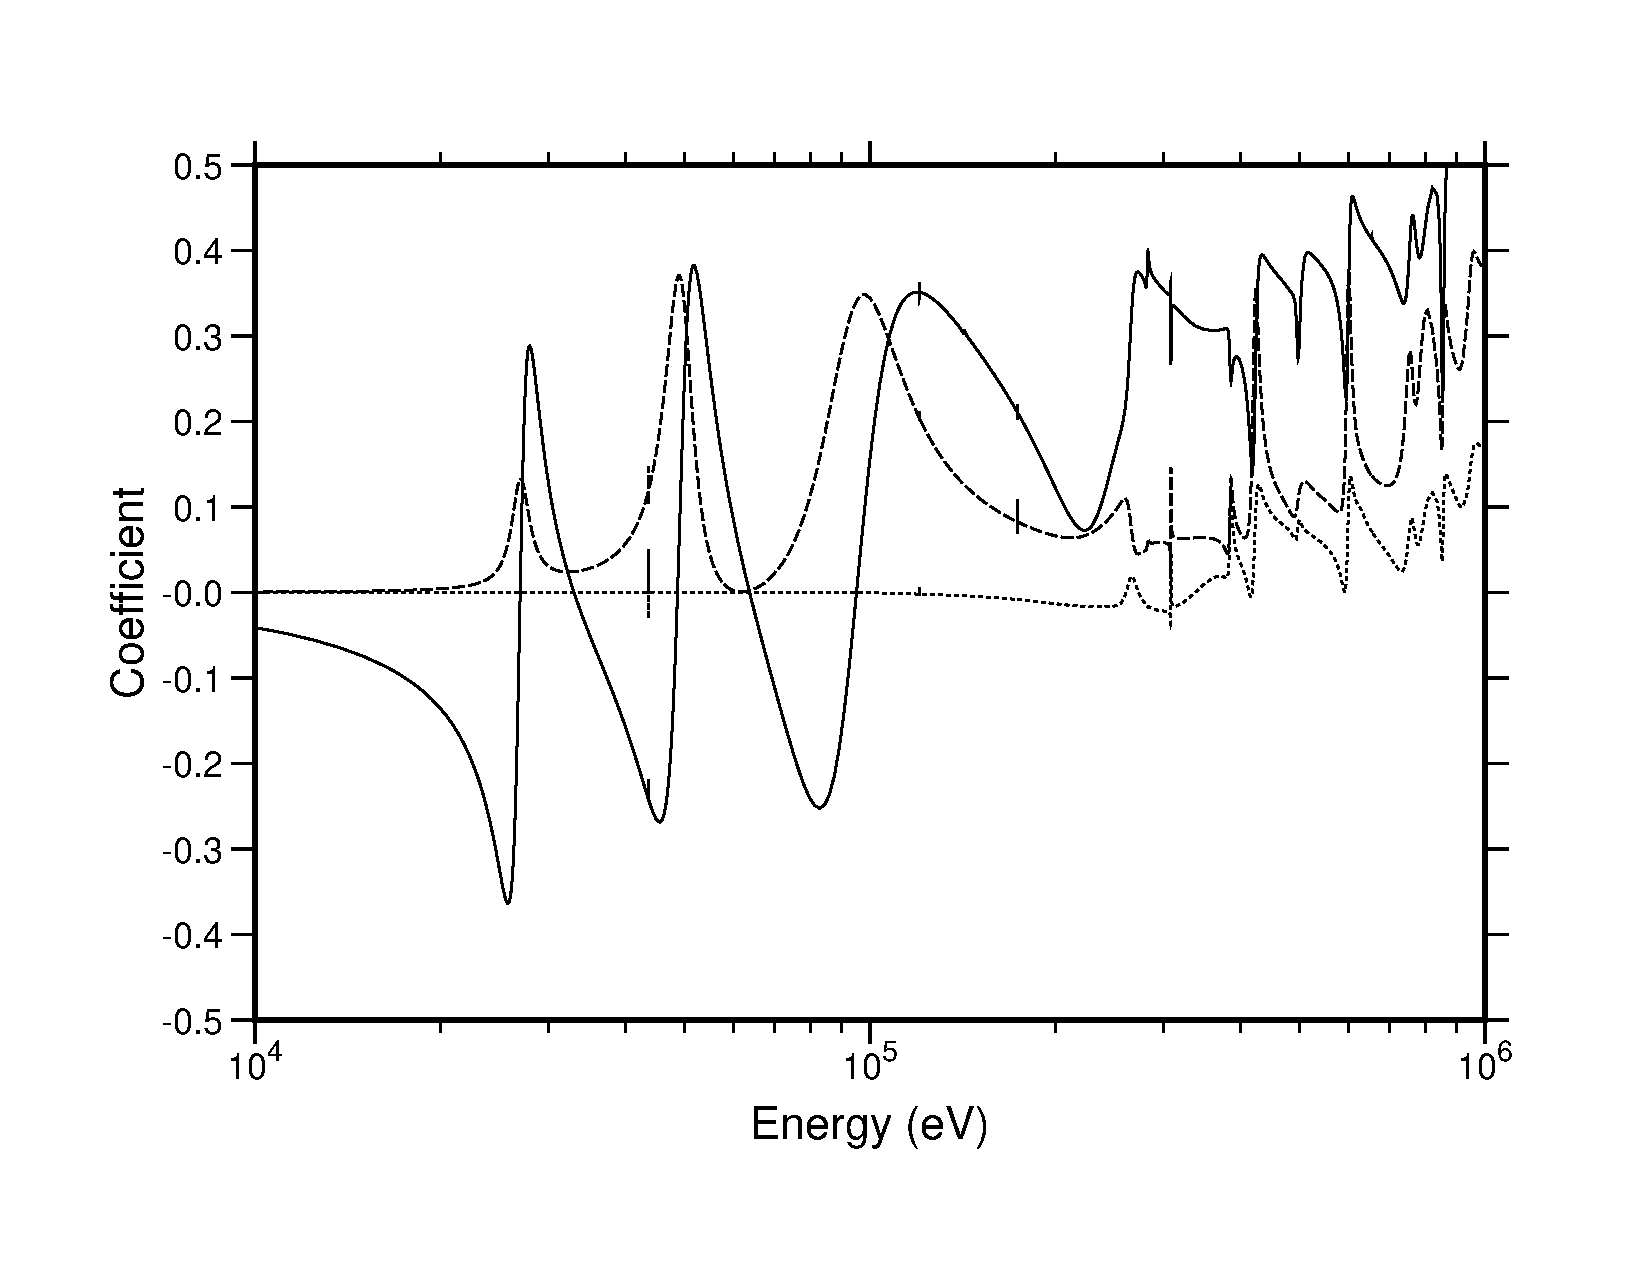
\includegraphics[height=3.5in, angle=0]{figs/adist_ack}
\caption[$^{19}$F elastic scattering Legendre coefficients from RML data]
  {Legendre coefficients of the angular distribution for
   elastic scattering in $^{19}$F using the RML resonance
   representation (P$_1$ solid, P$_2$ dashed, P$_3$ dotted).}
\label{adist}
\end{figure}

Although first introduced in NJOY2012, computing resonance
angular distributions is a new, little used feature, and so
it is not enabled by default.  To activate it, change
\cword{Want\_Angular\_Dist}\index{Want\_Angular\_Dist@{\ty Want\_Angular\_Dist}}
to true.  The Legendre coefficients are written into a section of
File 4 on the RECONR PENDF\index{PENDF} file.  Because the normal
ENDF File 4 sections are not copied to the PENDF File 4, the
presence of File 4 on a PENDF file can be detected by subsequent modules,
such a \hyperlink{sACERhy}{ACER}\index{ACER} or
\hyperlink{sGROUPRhy}{GROUPR}\index{GROUPR}, and the resonance
angular distributions can be used to replace the ENDF File 4 values
over the resonance energy range.  The default in NJOY2016 is to use
the conventional RM\index{Reich-Moore!RM} processing path for RM parameters.
However, there is an option to convert the RM parameters
into RML\index{Reich-Moore-Limited!RML} format and process them with the
RML methods.  If this is done, resonance angular distributions can be
computed for an RM evaluation.  Change \cword{Want\_SAMRML\_RM}
\index{Want\_SAMRML\_RM@{\ty Want\_SAMRML\_RM}} to true.

\paragraph{Infinitely-Dilute Unresolved Range Parameters}
Infinitely dilute cross sections in the unresolved-energy range
\index{unresolved resonance range} are computed in
\cword{csunr1}\index{csunr1@{\ty csunr1}} or
\cword{csunr2}\index{csunr2@{\ty csunr2}} using average
resonance parameters and probability distributions from File 2.
With the approximations used, these cross sections are not
temperature dependent; therefore, the results are a good match to
resolved resonance data generated using \cword{tempr}$>$0.  The
formulas used are based on the SLBW\index{Single-Level Breit-Wigner!SLBW}
approximation with interference.
\begin{eqnarray}
  \sigma_n (E) &=& \sigma_p
    +{\frac{2\pi^2}{k^2}} \sum_{\ell,J}
    {\frac{g_J}{\overline D}} \bigl[
    \overline\Gamma_n^2 R_n
    -2\overline\Gamma_n\sin^2\phi_\ell \bigr]
    \,\,,\\
  \sigma_x(E)&=&{\frac{2\pi^2}{k^2}}
    \sum_{\ell,J} {\frac{g_J}{\overline D}}
    \,\overline\Gamma_n \overline\Gamma_x R_x
    \,\,,\;\hbox{and}\\
  \sigma_p&=&{\frac{4\pi}{k^2}} \sum_\ell
    (2\ell+1)\sin^2\phi_\ell
    \,\,,
\end{eqnarray}
where $x$ stands for either fission or capture, $\overline
\Gamma_i$ and $\overline D$ are the appropriate average widths
and spacing for the $\ell{,}J$ spin sequence, and $R_i$ is the
fluctuation integral for the reaction and sequence (see
\cword{gnrl}).  These integrals are simply the averages taken
over the chi-square distributions\index{chi-square distributions}
specified in the file; for example,
\begin{eqnarray}
  \overline\Gamma_n\overline\Gamma_f R_i&=&
    \biggl< {\frac{\Gamma_n\Gamma_f}{\Gamma}} \biggr>\nonumber\\
  &=&\int dx_n P_\mu (x_n) \int dx_f P_\nu (x_f)
    \int dx_c P_\lambda (x_c)\,\\
  &\times&{\frac{\Gamma_n (x_n) \,\Gamma_f (x_f)}
    {\Gamma_n (x_n) + \Gamma_f (x_f) + \Gamma_\gamma
    +\Gamma_c (x_c)}}\,\,,
\end{eqnarray}
where $P_\mu(x)$ is the chi-square distribution for $\mu$
degrees of freedom.  The integrals are evaluated with the
quadrature scheme developed by R. Hwang for the MC$^2$-2
code\cite{MC22}\index{Hwang} giving
\begin{equation}
  R_f=\sum_i W_i^\mu\sum_j W_j^\nu\sum_k W_k^\lambda
    \,{\frac{Q_i^\mu\,Q_j^\nu}
    {\overline\Gamma_n Q_i^\mu + \overline\Gamma_f Q_j^\nu
    +\Gamma_\gamma+\overline\Gamma_c Q_k^\lambda}} \,\,.
\end{equation}
The $W_i^\mu$ and $Q_i^\mu$ are the appropriate quadrature
weights and values for $\mu$ degrees of freedom, and
$\Gamma_\gamma$ is assumed to be constant (many degrees of
freedom).  The competitive width\index{competitive width}
$\overline\Gamma_c$ is assumed to affect the fluctuations,
but a corresponding cross section is not computed.  The
entire competitive cross section is supposed to be in the
File 3 total cross section as a smooth background.

It should be noted that the reduced average neutron width
$\Gamma_n^0$ (AMUN) is given in the file, and
\begin{equation}
  \overline\Gamma_n=\Gamma_n^0\sqrt{E}\,V_\ell(E)\,\,,
\end{equation}
where the penetrabilities for the unresolved region are
defined as
\begin{eqnarray}
  V_0&=&1\,\,,\\
  V_1&=&{\frac{\rho^2}{1+\rho^2}}\,\,,\;\hbox{and}\\
  V_2&=&{\frac{\rho^4}{\rho+3\rho^2+\rho^4}}\,\,.
\end{eqnarray}
Other parameters are defined as for SLBW.

Unresolved resonance parameters can be given as independent
of energy, with only fission widths dependent on energy, or
as fully energy dependent.  The first two options are
processed in \cword{csunr1}, and the last one is processed
in \cword{csunr2}.

\subsection{Code Description}
\label{ssRECONR_details}

RECONR is implemented as a public subroutine
\cword{reconr}\index{reconr@{\ty reconr}}
exported by the Fortran-90 module
\cword{reconm}\index{modules!reconm@{\ty reconm}} defined by
\cword{reconr.f90}.

The first step is to read cards 1, 2, and 3 of the user's input.
The TAPEID record of the input file (\cword{nendf}) is read and
printed, then the new TAPEID record is written to the output
file (\cword{npend}).  RECONR is now ready to enter the loop
over the desired materials.
\index{TAPEID@{\ty TAPEID}}

For each material, space is allocated for the energy nodes
(\cword{enode}), and \cword{ruin}\index{ruin@{\ty ruin}}
is called to read cards 4 through 7 of the user's input.  If
the reconstruction temperature (\cword{tempr}) is greater than
zero, a table of $\psi$ and $\chi$ functions is generated
(the W table is used; see \cword{wtab}\index{wtab@{\ty wtab}}
and \cword{quickw}\index{quickw@{\ty quickw}}).  The
\cword{findf}\index{findf@{\ty findf}} utility routine from
module \cword{endf}\index{modules!endf@{\ty endf}} is then
used to find the first card of File 1 (MF=1, MT=451) for the
desired material.

File 1 on the input ENDF file is examined to obtain certain
constants and flags and to analyze the directory
(\cword{anlyzd}\index{anlyzd@{\ty anlyzd}}).
Subroutine \cword{anlyzd} determines which reactions should be
considered ``redundant''; that is, the reactions that are sums of
other reactions and will be included on the output PENDF file.
\index{redundant reactions}
\index{summation reactions}
The total cross section (MT=1 for neutrons, MT=501 for photons)
will always be included; the nonelastic cross section (MT=3) will
be included if it is needed for photon production (that is,
MF=12, MT=3 is found); the inelastic cross section (MT=4) will be
included if sections with MT in the range 51 -- 91 occur in the
file, and the total fission reaction (MT=18) will be called
redundant if the partial fission representation (MT=19, 20, 21,
38) is found.  MT103 (n,p) can be a summation reaction if its
partials MT600, MT601, ..., are present, and the same for the other
charged-particle absorption reactions.  Space for the new
material directory is then allocated (\cword{mfs}, \cword{mts},
\cword{ncs}).  Section identification and card counts will be
entered into these arrays as they are determined.

File 2 on the ENDF file is now checked using
\cword{s2sammy}\index{s2sammy@{\ty s2sammy}}
(which was imported from the \cword{samm}
module\index{modules!samm@{\ty samm}}) to see
whether the sammy method is needed.  This depends on whether
RML\index{Reich-Moore-Limited!RML} resonance parameters are found,
and whether conversion to RML format has been requested for
Reich-Moore or Breit-Wigner data (see
\cword{Want\_SAMRML\_RM}\index{Want\_SAMRML\_RM@{\ty Want\_SAMRML\_RM}}
and \cword{Want\_SAMRML\_BW}\index{Want\_SAMRML\_BW@{\ty Want\_SAMRML\_BW}}).
The variable \cword{nmtres} flags the use of SAMMY processing.
Because RML evaluations can include more than the normal elastic,
fission, and capture reactions, a list of reactions identified
is printed.  Here is an example from an experimental $^{19}$F evaluation.

\small
\begin{ccode}

 resonance range information
 ----------------------------------
 ier     energy-range     lru lrf  method
  1  1.000E-05 1.000E+06   1   7   sammy

   samm resonance reactions:    2  102   51   52
   samm max legendre order:  7
   generating File 4 for resonance angular distributions

\end{ccode}
\normalsize

The next step is to read File 2, which contains resolved and
unresolved resonance parameters (if any).  The array \cword{res}
is allocated to contain the File 2 data and
\cword{rdfil2}\index{rdfil2@{\ty rdfil2}} is called to read
them.  This routine uses the additional routines
\cword{rdf2bw}\index{rdf2bw@{\ty rdf2bw}},
\cword{rdf2aa}\index{rdf2aa@{\ty rdf2aa}},
\cword{rdf2hy}\index{rdf2hy@{\ty rdf2hy}},
\cword{rdsammy}\index{rdsammy@{\ty rdsammy}},
\cword{rdf2u0}\index{rdf2u0@{\ty rdf2u0}},
\cword{rdf2u1}\index{rdf2u1@{\ty rdf2u1}}, and
\cword{rdf2u2}\index{rdf2u2@{\ty rdf2u2}} to read the
different types of resonance parameters.  The subroutine
\cword{rdsammy} is imported from the
\cword{samm}\index{modules!samm@{\ty samm}} module.  In
addition, another imported routine
\cword{ppsammy}\index{ppsammy@{\ty ppsammy}} is used to
prepare for the SAMMY calculation.  While the resonance parameters
are being stored, RECONR  adds each resonance energy to its list
of energy nodes (\cword{enode}).  In the unresolved energy range,
RECONR uses the energies of tabulated parameters or fission widths
if available.  If the evaluation uses energy-independent parameters,
or if the energy steps between the nodes are too large (see
\cword{wide}\index{wide@{\ty wide}}), \cword{rdfil2} creates
additional node energies at a density of approximately 13 points
per decade (see \cword{egridu}).  Note that regions where the unresolved
representation for an element overlaps the resolved or smooth
ranges are found and marked by negative energy values.  The
energy nodes are sorted into order and duplications are removed.

If the SAMMY method is active, and if angular distributions
have been requested (see
\cword{Want\_Angular\_Dist}),
\index{Want\_Angular\_Dist@{\ty Want\_Angular\_Dist}}the maximum
Legendre order defined by the resonance data is printed out.

If unresolved data are present, subroutine
\cword{genunr}\index{genunr@{\ty genunr}} is called to compute
the infinitely-dilute unresolved average cross
sections on the unresolved energy grid using
\cword{csunr1}\index{genunr@{\ty genunr}} or
\cword{csunr2}\index{csunr1@{\ty csunr1}}.  Any backgrounds
on File 3 are included, except in regions of resolved-unresolved
or unresolved-smooth overlap.  The computed cross sections are
arranged in the order required by the special section with
MF=2 and MT=152, which is written onto the PENDF\index{PENDF}
tape by \cword{recout}\index{recout@{\ty recout}}.  Using the
normal ENDF style, this format is defined by the following:

\small
\begin{ccode}

    [MAT,2,152/ZA,AWR,LSSF,0,0,INTUNR]HEAD
    [MAT,2,152/0.,0.,5,1,NW,NUNR/
               E1,STOT1,SELAS1,SFIS1,SCAP1,STRN1,
               E2,STOT2,SELAS2,SFIS2,SCAP2,STRN2,
               ...
               ENUNR,STOTNUNR,....]LIST

\end{ccode}
\normalsize

\noindent
where \cword{NW} = 6 + 6*NUNR.  The definitions of the energy
and cross section entries are fairly obvious, except
\cword{STRN} stands for the current-weighted total cross
section.  This format is specialized to ``infinite
dilution.''  The more general form used for self-shielded
effective cross sections will be described in the
\hyperlink{sUNRESRhy}{UNRESR}\index{UNRESR},
\hyperlink{sPURRhy}{PURR}\index{PURR}, and
\hyperlink{sGROUPRhy}{GROUPR}\index{GROUPR}
chapters of this manual.

The subroutine \cword{lunion}\index{lunion@{\ty lunion}} is
used to linearize and unionize the ENDF data.  Space is reserved
for two buffers to be used by \cword{loada/finda}, for the
linearization stack (\cword{x} and \cword{y}), and for the
ENDF scratch area (\cword{scr}).  The length of the stack (\cword{ndim})
determines the smallest possible subdivision of each panel
(energy points as close as $2^{-{\mathtt{ndim}}}$ times the panel
width can be generated).  Since the number of energies in the
union grid may soon exceed the capacity of any reasonable memory
array, the existing list of energy nodes is copied to binary
scratch storage (the \cword{loada/finda} system).  This storage system
consists of the buffers \cword{bold} and \cword{bnew} and the
scratch units \cword{iold} and \cword{inew}.  The energy grid
points will ``ping-pong'' back and forth between units 14 and 15
as the union grid is built up.  Subroutine \cword{lunion} now
starts with MT=2 and checks each reaction in sequence to
determine whether the current grid (on \cword{iold}) is
sufficient to represent the reaction to within the desired
tolerance using linear interpolation.  If not, RECONR adds
additional points by adaptively halving the intervals.  The
new grid is stored on \cword{inew}.  The units \cword{inew} and
\cword{iold} are swapped, and the next MT is processed.  When all
nonredundant reactions have been examined, the list of energies
in \cword{loada/finda} storage is the desired linearized and
unionized grid.  The storage used is deallocated.

This grid is used as the starting point for resonance
reconstruction in \cword{resxs}\index{resxs@{\ty resxs}}.
Subroutine \cword{resxs} first reserves space for the
\cword{loada/finda} buffers \cword{bufr}
and \cword{bufg}, the linearization stack (\cword{x} and
\cword{y}), and the partial cross sections (\cword{sig}).  The
length of the stack (\cword{ndim}) determines the smallest
possible subdivision of a panel between two nodes (energy points
as close a $2^{-{\mathtt{ndim}}}$ times the panel width can be
generated).  Subroutine \cword{resxs} then examines the grid on
\cword{ngrid} (\cword{iold} from
\cword{lunion}\index{lunion@{\ty lunion}}) panel by panel.
Grid points are added and cross sections computed until the
convergence criteria discussed in Section \ref{ssRECONR_linear} are
satisfied.  The cross sections are copied to \cword{nout} using
\cword{loada}, and \cword{resxs} continues to the next panel.  This
procedure is continued until all panels are converged.  The result is a tape
(\cword{nout}) containing the energy grid in the resonance region
and the total, elastic, fission, capture, and possibly additional
cross sections at each energy point.

Unionization is obtained automatically in the resonance region
since all of the partials are computed simultaneously in
\cword{sigma}\index{sigma@{\ty sigma}}, using
\cword{csslbw}\index{csslbw@{\ty csslbw}} for SLBW\index{Single-Level
Breit-Wigner!SLBW} parameters, \cword{csmlbw}\index{csmlbw@{\ty csmlbw}}
for MLBW \index{Multi-Level Breit-Wigner!MLBW} parameters,
\cword{csaa}\index{csaa@{\ty csaa}} for multi-level Adler-Adler
\index{Adler-Adler} parameters,
\cword{csrmat}\index{csrmat@{\ty csrmat}} for Reich-Moore
\index{Reich-Moore!RM} parameters,
\cword{cshyb}\index{cshyb@{\ty cshyb}} for Hybrid R-Function
\index{Hybrid R-Function!HRF} parameters,
\cword{cssammy}\index{cssammy@{\ty cssammy}} for
Reich-Moore-Limited\index{Reich-Moore-Limited!RML} parameters,
and \cword{sigunr}\index{sigunr@{\ty sigunr}} for
unresolved resonance parameters.  This last routine retrieves
the cross sections from the table prepared by
\cword{genunr}\index{genunr@{\ty genunr}}.  Subroutine
\cword{cssammy} is imported from the \cword{samm}
module\index{modules!samm@{\ty samm}}.  A special feature
of RECONR is the ability to reconstruct
the cross sections at \cword{tempr} by $\psi\chi$
broadening\index{$\psi\chi$ broadening}
if SLBW\index{Single-Level Breit-Wigner!SLBW}
or Adler-Adler parameters are given.  This can also be done
for MLBW\index{Multi-Level Breit-Wigner!MLBW} using the GH
method\index{Multi-Level Breit-Wigner!GH MLBW method} implemented
by \cword{csmlbw2}\index{csmlbw2@{\ty csmlbw2}}.  The
Doppler-broadened resonance shapes are obtained using
\cword{quickw}\index{quickw@{\ty quickw}} (see description in
the \hyperlink{sUNRESRhy}{UNRESR}\index{UNRESR} chapter), and
the linearization procedure proceeds as before.

The resonance cross sections on \cword{ngrid} are merged with the
ENDF cross sections in \cword{emerge}\index{emerge@{\ty emerge}}.
First, the background grid from
\cword{lunion}\index{lunion@{\ty lunion}} is merged with the
resonance grid from \cword{resxs}\index{resxs@{\ty resxs}} and
written onto the \cword{loada/finda} file, which will
accumulate the total cross section and any other
redundant reactions required (\cword{iold/inew}).  A loop is then
set up over all nonredundant reactions.  For each grid point, the
ENDF background cross section is obtained by interpolation.  If
this grid point has a resonance contribution on \cword{nres}, it
is added.  The resulting net cross section at this point is added
into the appropriate redundant cross sections on
\cword{iold/inew} and also saved on \cword{ngrid}.  When all the
energies for this reaction have been processed, the cross
sections on \cword{ngrid} are converted into a TAB1 record and
written on \cword{nscr}.  This loop is continued until all
reactions have been processed.  When \cword{emerge} is finished,
\cword{nscr} contains cross sections for all the nonredundant
reactions, and \cword{iold} contains the redundant summation
reactions.

Control now passes to \cword{recout}\index{recout@{\ty recout}},
which writes the new File 1 comments and dictionary.  It also
writes a default version of the section with MF=2 and  MT=151
that gives no resonance parameters.  The upper limit
of the resolved energy range, \cword{eresh}, is added to the
``C2'' field of the third card so that \hyperlink{sBROADRhy}{BROADR}
\index{BROADR} knows
not to broaden into the unresolved energy range.  For materials with
unresolved data, a specially formatted section (MF=2, MT=152) is
written containing the infinitely-dilute unresolved cross
sections.  This section can be used by \hyperlink{sBROADRhy}{BROADR}
and \hyperlink{sGROUPRhy}{GROUPR}\index{GROUPR}
to correct for resolved-unresolved overlap effects, if necessary.
Subroutine \cword{recout} then steps through the reactions on
\cword{nscr} and \cword{iold}.  Redundant summation reactions
are converted to TAB1 records and inserted in the correct order.
Nonredundant reactions are simply copied.  Finally, a MEND
record is added and control is returned to \cword{reconr}.

Now \cword{reconr} either directs that this process be repeated
for another isotope or writes a TEND record and terminates.  The
result is a new file in ENDF format containing the desired
pointwise cross sections.  Normally, only Files 1, 2, 3, 10, and
13 are included for neutron files.  However, if angular
distribution processing has been requested, a File 4 containing
the Legendre coefficients will also be written.  Because the
original ENDF File 4 was not copied to the PENDF file, the
presence of sections of File 4 on the PENDF file provides a
flag to subsequent modules that resonance angular distributions
\index{resonance angular distributions} have been calculated.
Only Files 1 and 23 are included for a photon file.

The SAMMY method is implemented in a separate Fortran-90
module \cword{samm}\index{modules!samm@{\ty samm}}
defined by \cword{sammy.f90}.  It exports the subroutines
\cword{cssammy}\index{cssammy@{\ty cssammy}} (computes cross
sections, angular distributions, and derivatives),
\cword{s2sammy}\index{s2sammy@{\ty s2sammy}} (scans File 2
to see if SAMMY method is needed and measure some sizes),
\cword{ppsammy}\index{ppsammy@{\ty ppsammy}} (sets up SAMMY
calculation), \cword{rdsammy}\index{rdsammy@{\ty rdsammy}}
(reads in File 2 data with optional conversion of
BW\index{Single-Level Breit-Wigner!SLBW}
\index{Multi-Level Breit-Wigner!MLBW}
or RM\index{Reich-Moore!RM} data to
RML\index{Reich-Moore-Limited!RML} form), and
\cword{desammy}\index{desammy@{\ty desammy}}
(cleans up after the SAMMY calculation).  It also exports some
logical parameters, namely,
\cword{Want\_Partial\_Derivs},
\index{Want\_Partial\_Derivs@{\ty Want\_Partial\_Derivs}}
\cword{Want\_Angular\_Dist},
\index{Want\_Angular\_Dist@{\ty Want\_Angular\_Dist}}
\cword{Want\_SAMRML\_RM}
\index{Want\_SAMRML\_RM@{\ty Want\_SAMRML\_RM}} and
\cword{Want\_SAMRML\_BW}.
\index{Want\_SAMRML\_BW@{\ty Want\_SAMRML\_BW}}  See
\hyperlink{sERRORRhy}{ERRORR}\index{ERRORR} for the use
of derivatives.  If conversion from
BW and/or RM was requested, it is possible to get the
resulting File 2 values printed out for checking.  Just
set \cword{imf2} in \cword{sammy.f90} to 1.

The \cword{cssammy}\index{cssammy@{\ty cssammy}} subroutine
uses \cword{abpart}\index{abpart@{\ty bpart}} to compute
some energy-independent pieces of the cross sections and
derivatives.  The main work for cross sections, angular
distributions, and derivatives in done in
\cword{cross}\index{cross@{\ty cross}}.  The
results for cross sections are returned in
\cword{sigp}\index{sigp@{\ty sigp}} to be
consistent with the other ``cs'' routines in RECONR.  Angular
distributions are returned in \cword{siga}, and sensitivities
are returned in \cword{sigd} (derivatives of cross sections
with respect to parameters).  Subroutine
\cword{cross}\index{cross@{\ty cross}} starts
by initializing the quantities being calculated (cross sections,
maybe angular distributions, maybe derivatives), and then it
sets up a loop over the spin-parity groups.  It initializes the
results for this spin group and then calls
\cword{setr}\index{setr@{\ty setr}} to compute the elements
of the R-matrix\index{R-matrix} (see Eq.~\ref{rmtx} and other
quantities, such as the Y matrix, penetrabilities
(\cword{rootp}), and phase shifts.  It then inverts the
Y matrix and calculates the X matrix of Eq.~\ref{xmtx}.
See \cword{setxqx}.  It can then use the X matrix to compute
the contributions to the cross sections (\cword{sectio}),
maybe angular distributions (\cword{setleg}), and maybe
derivatives from this spin group and add them into the sum
over groups.  When the loop over spin groups is complete,
it normalizes things properly and returns its results.

Going back to subroutine \cword{setr}, it computes the R-matrix
first.  It then computes the phase shift, penetrabilities, and
shift factors.  For non-Coulomb cases, the phase shifts come
from \cword{sinsix}, and the penetrability $P$ and boundry
condition $(S-B+iP)^{-1}$ come from \cword{pgh}.  For Coulomb
cases, subroutine \cword{pghcou}
\noindent computes all of these
quantities.  The penetrability $P$ is converted to \cword{rootp}
for use in Eq.~\ref{xmtx}.

\subsection{Input Instructions}
\label{ssRECONR_inp}

The input instructions for each module are given in the code
as comment cards at the beginning of the source code for each
module.  The RECONR instructions are reproduced here for the
convenience of the reader.
\index{RECONR!RECONR input}
\index{input!RECONR}

\small
\begin{ccode}

   !---input specifications (free format)---------------------------
   !
   ! card 1
   !    nendf    unit for endf tape
   !    npend    unit for pendf tape
   ! card 2
   !    tlabel   66 character label for new pendf tape
   !             delimited with quotes, ended with /.
   ! card 3
   !    mat      material to be reconstructed
   !    ncards   number of cards of descriptive data for new mf1
   !             (default=0)
   !    ngrid    number of user energy grid points to be added.
   !             (default=0)
   ! card 4
   !    err      fractional reconstruction tolerance used when
   !             resonance-integral error criterion (see errint)
   !             is not satisfied.
   !    tempr    reconstruction temperature (deg kelvin)
   !             (default=0)
   !    errmax   fractional reconstruction tolerance used when
   !             resonance-integral error criterion is satisfied
   !             (errmax.ge.err, default=10*err)
   !    errint   maximum resonance-integral error (in barns)
   !             per grid point (default=err/20000)
   !             (note: the max cross section difference for
   !             linearization, errlim, and for reconstruction,
   !             errmin, are also tied to errint.  to get maximum
   !             accuracy, set errint to a very small number.
   !             for economical production, use the defaults.)
   ! card 5
   !    cards    ncards of descriptive comments for mt451
   !             each card delimited with quotes, ended with /.
   ! card 6
   !    enode    users energy grid points
   !
   !     cards 3, 4, 5, 6 must be input for each material desired
   !     mat=0/ terminates execution of reconr.
   !
   !-------------------------------------------------------------------

\end{ccode}
\normalsize

\noindent
A sample input for processing an isotope from ENDF/B-VII
follows (the line numbers are for reference only and are not
part of the input).  First, mount the ENDF/B-VII file for
$^{235}$U on unit 20.

\small
\begin{ccode}

   1.  reconr
   2.  20 21/
   3.  'pendf tape for U-235 from ENDF/B-VII'/
   4.  9228 2/
   5.  .001/
   6.  '92-U-235 from ENDF/B-VII'/
   7.  'processed with NJOY'/
   8.  0/

\end{ccode}
\normalsize

Card 2 tells RECONR that the input ENDF tape will be
on unit 20, and that the output PENDF tape will be on unit 21.
Card 3 is a ``TAPEID'' label for the output PENDF file.
Card 4 gives the MAT number for U-235 and says that two
additional comment cards will be given.  Card 5 sets the
reconstruction tolerance to 0.1\% (.001 as a fraction)
with all its other parameters defaulted.  Cards 6 and 7
are the two comment cards to be inserted into the PENDF
files MF1/MT451 section.  Finally, the ``0/'' terminates the
RECONR input.  The capability to loop over multiple isotopes
in RECONR is rarely used for neutron files, but it is
useful for photon interaction processing (see GAMINR).
The resulting PENDF tape will contain the desired TAPEID
card, followed by $^{235}$U data, a MEND card and a TEND card.


\subsection{Error Messages}
\label{ssRECONR_msg}

\begin{description}
\begin{singlespace}

\item[\cword{error in reconr***illegal nsub for reconr}] ~\par
   RECONR only processes sublibraries that contain cross section
   data.  Check whether the right input ENDF input tape was
   mounted.

\item[\cword{error in anlyzd***too many redundant reactions}] ~\par
   Increase the global parameter \cword{nmtmax}=10.

\item[\cword{error in xxxxxx***storage in enode exceeded}] ~\par
   Too many energy nodes including the user's nodes and
   the energies from MF=2.  Increase the global parameter
   \cword{nodmax}=800000.  This message can come from \cword{rdf2bw},
   \cword{rdf2aa}, \cword{rdf2hy}, \cword{rdf2u0}, \cword{rdf2u1},
   or \cword{rdf2u2}.

\item[\cword{error in xxxxxx***res storage exceeded}] ~\par
   Too much resonance data.  This should not occur for a conforming
   ENDF-format file, because \cword{maxres} is computed from the
   MF=2 line count in the MF=1/MT=451 index.
   This message can come from \cword{rdfil2}, \cword{rdf2bw},
   \cword{rdf2aa}, \cword{rdf2hy}, \cword{rdf2u0}, \cword{rdf2u1},
   or \cword{rdf2u2}.

\item[\cword{error in xxxxxx***storage in eunr exceeded.}] ~\par
   Increase the global parameter \cword{maxunr}=500.  This message can
   come from \cword{rdfil2}, \cword{rdf2u1}, or \cword{rdf2u2}.

\item[\cword{error in rdfil2***illegal resonance mode.}] ~\par
   A resonance mode has been requested that RECONR does not understand.

\item[\cword{error in rdf2bw***energy-dep scattering radius ...}] ~\par
   This option is only used in MLBW for current evaluations.

\item[\cword{message from rdf2bw***calc... of angular distribution not... }]
 ~\par This option is only partially available in RECONR.  This message can
 come from \cword{rdf2bw} (for Reich-Moore cases) or from \cword{rdf2hy}
 (Hybrid R function).

\item[\cword{error in rdf2hy***hybrid competing reactions not yet added}] ~\par
   This option is not yet available in RECONR.

\item[\cword{error in lunion***ill behaved threshold}] ~\par
   The routine is having trouble adjusting the threshold to
   agree with the Q value.  Check the points near the threshold
   for this evaluation.

\item[\cword{error in lunion***exceeded stack}] ~\par
   Increase length of linearization stack \cword{ndim} (currently 50).

\item[\cword{error in resxs***stack exceeded}] ~\par
   Increase length of reconstruction stack \cword{ndim} (currently 50).

\item[\cword{error in sigma***general r-matrix not installed.}] ~\par
   This option is not yet available in RECONR.

\item[\cword{error in sigma***illegal option.}] ~\par
   There is a problem with the ENDF tape.

\item[\cword{error in csmlbw***not coded for temperature gt 0 deg k}] ~\par
   The $\psi\chi$ Doppler-broadening doesn't work for normal
   MLBW.  This message shouldn't occur, because temperatures
   greater than zero will cause \cword{csmlbw2} to be called.

\item[\cword{error in csrmat***not coded for temperature gt 0 deg k}] ~\par
   The $\psi\chi$ Doppler-broadening doesn't work for RM.
   Use \cword{tempr}=0. only.

\item[\cword{error in cshybr***doppler broad'g not provided for hybrid}] ~\par
   The $\psi\chi$ Doppler-broadening doesn't work for hybrid
   parameters.  Use \cword{tempr}=0. only.

\item[\cword{error in csaa***bad li value}] ~\par
   There is an error in the evaluation format.

\item[\cword{message from emerge---negative elastic cross sects found}] ~\par
   Negative elastic cross sections can occur for SLBW evaluations.

\item[\cword{error in recout***for mf --- mt ---}] ~\par
    Indexing and pair count for this section do not make sense.

\item[\cword{calculation of angular distribution not installed}] - \par
   Message comes from several resonance types that do not
   support the calculation of angular distributions.  Some
   of them can be used if \cword{Want\_SAMRL\_RM} or
   \cword{Want\_SAMRML\_BW} are true.

\item[\cword{message from s2sammy***multiple isotopes...}] -
\par
   Multiple isotopes for RM sections don't work with the SAMMY
   method.  The code automatically reverts to normal RM
   processing.

\item[\cword{error in s2sammy***res storage exceeded.}] -
\par
  Storage limited to \cword{maxres}.  Shouldn't occur.

\item[\cword{error in s2sammy***energy-dep scattering length...}] -
\par
  This only works for MLBW parameters.

\item[\cword{error in rearrange***nres fault}] -
\par
  Trouble while rearranging resonances into spin-group order.

\item[\cword{errorr in findsp***quantum numbers in file 2 do not...}] -
\par
  Problems with the quantum numbers for the evaluation.

\item[\cword{error in checkqn***error in quantum numbers}] -
\par
  Problems with the quantum numbers for the evaluation.

\item[\cword{error in lmaxxx***lllmax limit to 51}] -
\par
  Problems with the Clebsch-Gordan coefficients for the
  angular distributions.

\item[\cword{error in clbsch***did not count correctly}] -
\par
  Problems with the Clebsch-Gordan coefficients for the
  angular distributions.

\item[\cword{error in pspcou***llmax larger than 100}] -
\par
  Problem computing the Coulomb phase shifts.

\item[\cword{error in bigeta***I0 sum failed}] -
\par
  Problem for the Coulomb routine.

\item[\cword{error in bigeta***K0 sum failed}] -
\par
  Problem for the Coulomb routine.

\item[\cword{error in bigeta***L1 sum failed}] -
\par
  Problem for the Coulomb routine.

\item[\cword{error in bigeta***K1 sum failed}] -
\par
  Problem for the Coulomb routine.

\item[\cword{error in setleg***nppx too large}] -
\par
  Problem generating Legendre polynomials.

\end{singlespace}
\end{description}

\subsection{Input-Output Units}
\label{ssRECONR_IOunits}

The following logical units are used:

\begin{list}{}{\leftmargin=.75in\labelsep=.25in\labelwidth=.5in}
\begin{singlespace}

\item[10] \cword{nscr1} in \cword{reconr}, \cword{nout} in
          \cword{lunion}, and \cword{nin} in \cword{emerge}.
          Contains copy of nonredundant sections from original
          ENDF tape.
\item[11] \cword{nscr2} in \cword{reconr}; \cword{ngrid} in
          \cword{lunion}, \cword{resxs}, and \cword{emerge}.
          Contains union grid for ENDF tape (not counting
          resonances).
\item[12] \cword{nscr3} in \cword{reconr}, \cword{nout} in
          \cword{resxs}, and \cword{nres} in \cword{emerge}.
          Contains resonance grid and cross sections.
\item[13] \cword{nscr4} in \cword{reconr} is used for two separate
          purposes.  In \cword{resxs} it is a binary scratch file
          \cword{nscr} used for the unthinned resonance data.  In
          \cword{emerge} and \cword{recout}, it
          is \cword{nmerge} and contains the nonredundant reactions on
          the union grid.
\item[14/15] \cword{iold/inew} in \cword{lunion}.  Are used locally only
          to accumulate union grid for ENDF cross sections.
          Destroy after use.
\item[14/15] \cword{iold/inew} in \cword{emerge}.  Are used locally only
          to accumulate summation cross sections on union grid.
\item[20-99] User's choice for ENDF (\cword{nendf}) and PENDF (\cword{npend})
          tape numbers to link RECONR with other NJOY modules.
\item[5,6,7] See the \hyperlink{sNJOYhy}{NJOY} chapter for a
          description of the I/O units.

\end{singlespace}
\end{list}

\noindent
Note that 11, 12, 14, and 15 are always binary.  Unit 10 has the
same mode as \cword{nendf}.  Unit 13 is binary when used in RESXS, and
it has the same mode as \cword{npend} elsewhere.  \cword{npend} can have a
different mode than \cword{nendf}.

\subsection{Storage Allocation}
\label{ssRECONR_storage}

Storage allocation in RECONR is sensitive to (1) the amount of
resonance parameter data, (2) the number of energy-grid node
values, (3) the size of the resonance reconstruction stack,
(4) the use of $\psi\chi$ broadening, and \index{$\psi\chi$
broadening} (5) the sizes of the \cword{loada/finda} buffers.
Other storage requirements are minor.

Buffer sizes can be reduced or increased at will.  The result is
a storage/speed tradeoff with no change in capability or accuracy.
See the global parameters \cword{nbufg}=2000, \cword{nbufr}=2000,
and \cword{nbuf}=2000 at the beginning of the \cword{reconm} module.

The $\psi\chi$ broadening option requires 7688 words of
additional storage.  Therefore, memory use can be reduced
if $\psi\chi$ is not required.  No code changes
are needed --- just avoid \cword{tempr} greater than zero.

Resonance reconstruction in \cword{resxs} uses
5${\times}$\cword{ndim} words.  The parameter \cword{ndim}
determines the smallest subdivision of a panel that can be
obtained.  Using \cword{ndim}=30 allows points to be generated
with spacing as small as one-billionth of the panel size
($2^{30}$).

The code currently allows for \cword{nodmax}=800000 energy nodes
and \cword{maxunr}=500 unresolved points.  These values tend to
increase as additional very detailed resonance evaluations appear,
but the current values seem to be sufficient for the evaluations
existing as of this writing.

\cleardoublepage


\section{BROADR}
\label{sBROADR}

\hypertarget{sBROADRhy}{BROADR}
\index{BROADR|textbf} module generates
Doppler-broadened\index{Doppler-broadening}
cross sections in PENDF\index{PENDF} format starting from piecewise
linear cross sections in PENDF format.  The input cross sections can
be from \hyperlink{sRECONRhy}{RECONR}\index{RECONR} or
from a previous BROADR run.  The code is
based on SIGMA1\cite{SIGMA1}\index{SIGMA1} by D. E. Cullen.\index{Cullen}
The method is often called ``kernel broadening''\index{kernel broadening}
because it uses a detailed integration of the integral equation defining
the effective cross section.  It is a fully accurate method,
treating all resonance and non-resonance cross sections including
multilevel effects.  BROADR has the following features:
\begin{itemize}
\begin{singlespace}
\item An alternate calculation is used for low energies
      and high temperatures that corrects a numerical problem of
      the original SIGMA1. (This problem has been corrected
      in another way in later versions of SIGMA1.)

\item Dynamic storage allocation is used, which allows the code
      to be run on large or small machines with full use of whatever
      storage is made available.

\item Reactions are broadened in parallel on a union grid, with the top
      of the resolved resonance range being the typical upper limit
      for Doppler broadening.

\item The union grid is constructed adaptively to give
      a linearized representation of the broadened cross section
      with tolerances consistent with those used in
      \hyperlink{sRECONRhy}{RECONR}.  Energy
      points may be added to or removed from the
      input grid as required for the best possible
      representation.  Precision up to 9 significant figures
      is allowed for energies.

\item The summation cross sections such as total, nonelastic, and
      sometimes fission or (n,2n) are reconstructed to equal the
      sum of their parts.

\item Standard thermal cross sections, integrals, and ratios are
      computed when the temperature is 293.6K (0.0253 eV).

\item The file directory (actually an index to the
      reactions present) is updated.
\end{singlespace}
\end{itemize}

This chapter describes the BROADR module in NJOY2016.0.

\subsection{Doppler-Broadening Theory}
\label{ssBROADR_theory}

The effective cross section for a material at temperature $T$ is
defined to be that cross section that gives the same reaction rate
for stationary target nuclei as the real cross section gives for
moving nuclei.  Therefore,
\begin{equation}
  \rho v {\overline \sigma}(v,T)=
    \int d{\bf v}' \rho\,|{\bf v}-{\bf v}'|\,\sigma(|{\bf v}-{\bf v}'|
    )\,P({\bf v}',T)\,\,,
\label{effxs}
\end{equation}
where ${\bf v}$ is the velocity of the incident particles,
${\bf v}'$ is the velocity of the target, $\rho$ is the density
of target nuclei, $\sigma$ is the cross section for stationary
nuclei, and $P({\bf v}',T)$ is the distribution of target
velocities in the laboratory system.  For many cases of interest,
the target motion is isotropic and the distribution of velocities
can be described by the Maxwell-Boltzmann\index{Maxwell-Boltzmann function}
function
\begin{equation}
  P({\bf v}',T)\,d{\bf v}'=
    {{\alpha^{3/2}} \over {\pi^{3/2}}} \exp (-\alpha {v'}^2)\,
    d{\bf v}'\,\,,
\end{equation}
where $\alpha=M/(2kT)$, $k$ is Boltzmann's constant\index{Boltzmann
constant}, and $M$ is the target mass.

Eq.~\ref{effxs} can be partially integrated in terms of the
relative speed $V=|{\bf v}-{\bf v}'|$ to give the standard form
of the Doppler-broadened cross section:
\begin{equation}
  {\overline\sigma}(v)={{\alpha^{1/2}} \over {\phi^{1/2}\,v^2}}
    \int_0^\infty dV\,\sigma(V)\,V^2\,\Bigl\lbrace
    {\rm e}^{-\alpha (V-v)^2}-{\rm e}^{-\alpha (V+v)^2}
    \Bigr\rbrace \,\,.
\label{standform}
\end{equation}
It is instructive to break this up into two parts:
\begin{equation}
  {\overline\sigma}(v)=\sigma^* (v)-\sigma^*(-v)\,\,,
\end{equation}
where
\begin{equation}
  \sigma^*(v)={{\alpha^{1/2}} \over {\pi^{1/2}v^2}}
    \int_0^\infty dV\,\sigma(V)\,V^2\,{\rm e}
    ^{-\alpha (V-v)^2} \,\,.
\label{sigv}
\end{equation}

\noindent
The exponential function in Eq.~(\ref{sigv}) limits the
significant part of the integral to the range
\begin{displaymath}
  v-{{4}\over {\sqrt{\alpha}}} < V
    <v+{{4} \over {\sqrt{\alpha}}} .
\end{displaymath}
For $\sigma^*(-v)$, the integral depends only on velocities
satisfying
\begin{displaymath}
   0\le V<{{4}\over{\sqrt{\alpha}}} .
\end{displaymath}
These results can be converted to energy units using
\begin{displaymath}
E_m={1\over 2} m \bigl( {4 \over \sqrt{\alpha}} \bigr)^2
    = {{16kT} \over A}.
\end{displaymath}
Some examples are given in Table~\ref{T1}.  Doppler-broadening effects
will be important below this energy and for any features such as
resonances, thresholds, or artificial discontinuities in
evaluations that are not slowly varying with respect to
$2\sqrt{E_mE}$.  As an example, for $^{235}$U at 100 eV, Doppler
effects are important for features smaller than about 0.8 eV.

\begin{table}
\caption[Energy Parameter for Effective Doppler-Broadening]
 {Energy Parameter for Effective Doppler-Broadening}
\setlength{\extrarowheight}{1pt}
\label{T1}
\begin{center}
\begin{tabular}{lcc}
Target & Temperature & Energy Parameter ($E_m$) \\
\hline
$^{2}$H & 300K & 0.2 eV \\
$^{235}$U & 300K & 0.0017 eV \\
$^{235}$U & 1.0 keV & 69 eV \\
\hline
\end{tabular}
\end{center}
\end{table}

The numerical evaluation of Eq.~(\ref{sigv}) developed for SIGMA1
assumes that the cross section can be represented by a piecewise
linear function of energy to acceptable accuracy.  This is just
the form of the NJOY PENDF\index{PENDF} files (see
\hyperlink{sRECONRhy}{RECONR}\index{RECONR}).  Defining the
reduced variables $y=\sqrt{\alpha x}$ and $x=\sqrt{\alpha V}$,
the cross section becomes
\begin{equation}
  \sigma (x)=\sigma_i + s_i (x^2-x_i^2 )\,\,,
\label{sigmax}
\end{equation}
with slope $s_i=(\sigma_{i+1}-\sigma_i)/(x_{i+1}^2-x_i^2 )$.
Eq.~(\ref{sigv}) can now be written as
\begin{equation}
  \sigma^*(y)={{1} \over{\pi^{1/2}y^2}}
    \sum_{i=0}^N \int_{x_i}^{x_{i+1}}
    \sigma (x)\,x^2 {\rm e}^{-(x-y)^2}dx
    = \sum_i \bigl\lbrace A_i\,[\sigma_i-s_i x_i^2]+
    B_i s_i \bigr\rbrace \,\,,
\label{sigy}
\end{equation}
where
\begin{eqnarray}
  x_0&=&0\,\,,\nonumber\\
  x_{N+1}&=&\infty\,\,,\nonumber\\
  A_i&=&{1\over y^2}H_2+{2\over y}H_1+H_0\,\,,\;\hbox{and}\nonumber\\
  B_i&=&{1\over y^2}H_4+{4\over y}H_3+6H_2+4yH_1+y^2 H_0\nonumber \,\,,
\end{eqnarray}
and where $H_n$ is shorthand for $H_n(x_i{-}y,x_{i+1}{-}y)$.  The
extrapolations to zero and infinity assume a constant cross section
($s_0{=}s_N{=}0$).  The $H$ functions are the incomplete
probability integrals\index{incomplete probability integral}
\index{math!incomplete probability integral} defined by
\begin{equation}
  H_n(a,b)={1\over \sqrt{\pi}} \int_a^b
    z^n\,{\rm e}^{-z^2}\,dz\,\,.
\label{fn}
\end{equation}
These functions can be computed in two ways.  First,
\begin{equation}
  H_n(a,b)=F_n(a)-F_n(b)\,\,,
\label{diffs}
\end{equation}
where
\begin{equation}
  F_n(a)={1\over \sqrt{\pi}}\int_a^\infty z^n\,{\rm e}^{-z^2}\,dz\,\,.
\end{equation}
These functions satisfy a recursion relation that can be used
to obtain
\begin{eqnarray}
  F_0(a)&=&{1\over 2} {\rm erfc}(a)\,\,,\\
  F_1(a)&=&{1\over {2\sqrt{\pi}}} \exp(-a^2)\,\,,\;\hbox{and}\\
  F_n(a)&=&{{n-1} \over 2}F_{n-2}(a)+a^{n-1}F_1(a)\,\,,
\label{recur}
\end{eqnarray}
where ${\rm erfc}(a)$ denotes the complementary error function
\index{complementary error function}
\index{math!complementary error function}
\begin{equation}
  {\rm erfc}(a)={2\over \sqrt{\pi}}
    \int_a^\infty {\rm e}^{-z^2}dz\,\,.
\end{equation}
However, when $F_n(a)\approx F_n(b)$, the difference in
Eq.~(\ref{diffs}) may lose significance.  In such cases,
$H_n(a,b)$ can be computed by a second method based on a
direct Taylor expansion of the defining integral.  Write
\begin{equation}
  H_n(a,b)={1\over \sqrt{\pi}}\int_0^b z^n {\rm e}^{-z}
    dz-{1\over \sqrt{\pi}}\int_0^a z^n {\rm e}^{-z^2}dz
    =G_n(b)-G_n(a)\,\,.
\label{alt1}
\end{equation}
But by Taylor's Theorem,
\begin{equation}
  G_n(b)-G_n(a)=
    {{b-a}\over {1!}}G'_n(a)+...+
    {{(b-a)^m}\over{m!}}G_n^{(m)}(a)+... \,.
\end{equation}
Also,
\begin{equation}
  G_n^{(m)}(x)={{d^{m-1}}\over{dx^{m-1}}}
    \bigl[ x^n{\rm e}^{-x^2} \bigr] =
    {\rm e}^{-x^2} P_n^m(x)\,,
\end{equation}
where $P_n^m(x)$ is a polynomial with recursion relation
\begin{equation}
  P_n^m(x)={d\over{dx}}P_n^{m-1}(x)-2xP_n^{m-1}(x)\,\,,
\label{alt2}
\end{equation}
with $P_n^1=x^n$.  From this point, it is straightforward to
generate terms until the desired number of significant figures
is obtained.

\begin{figure}[t]\centering
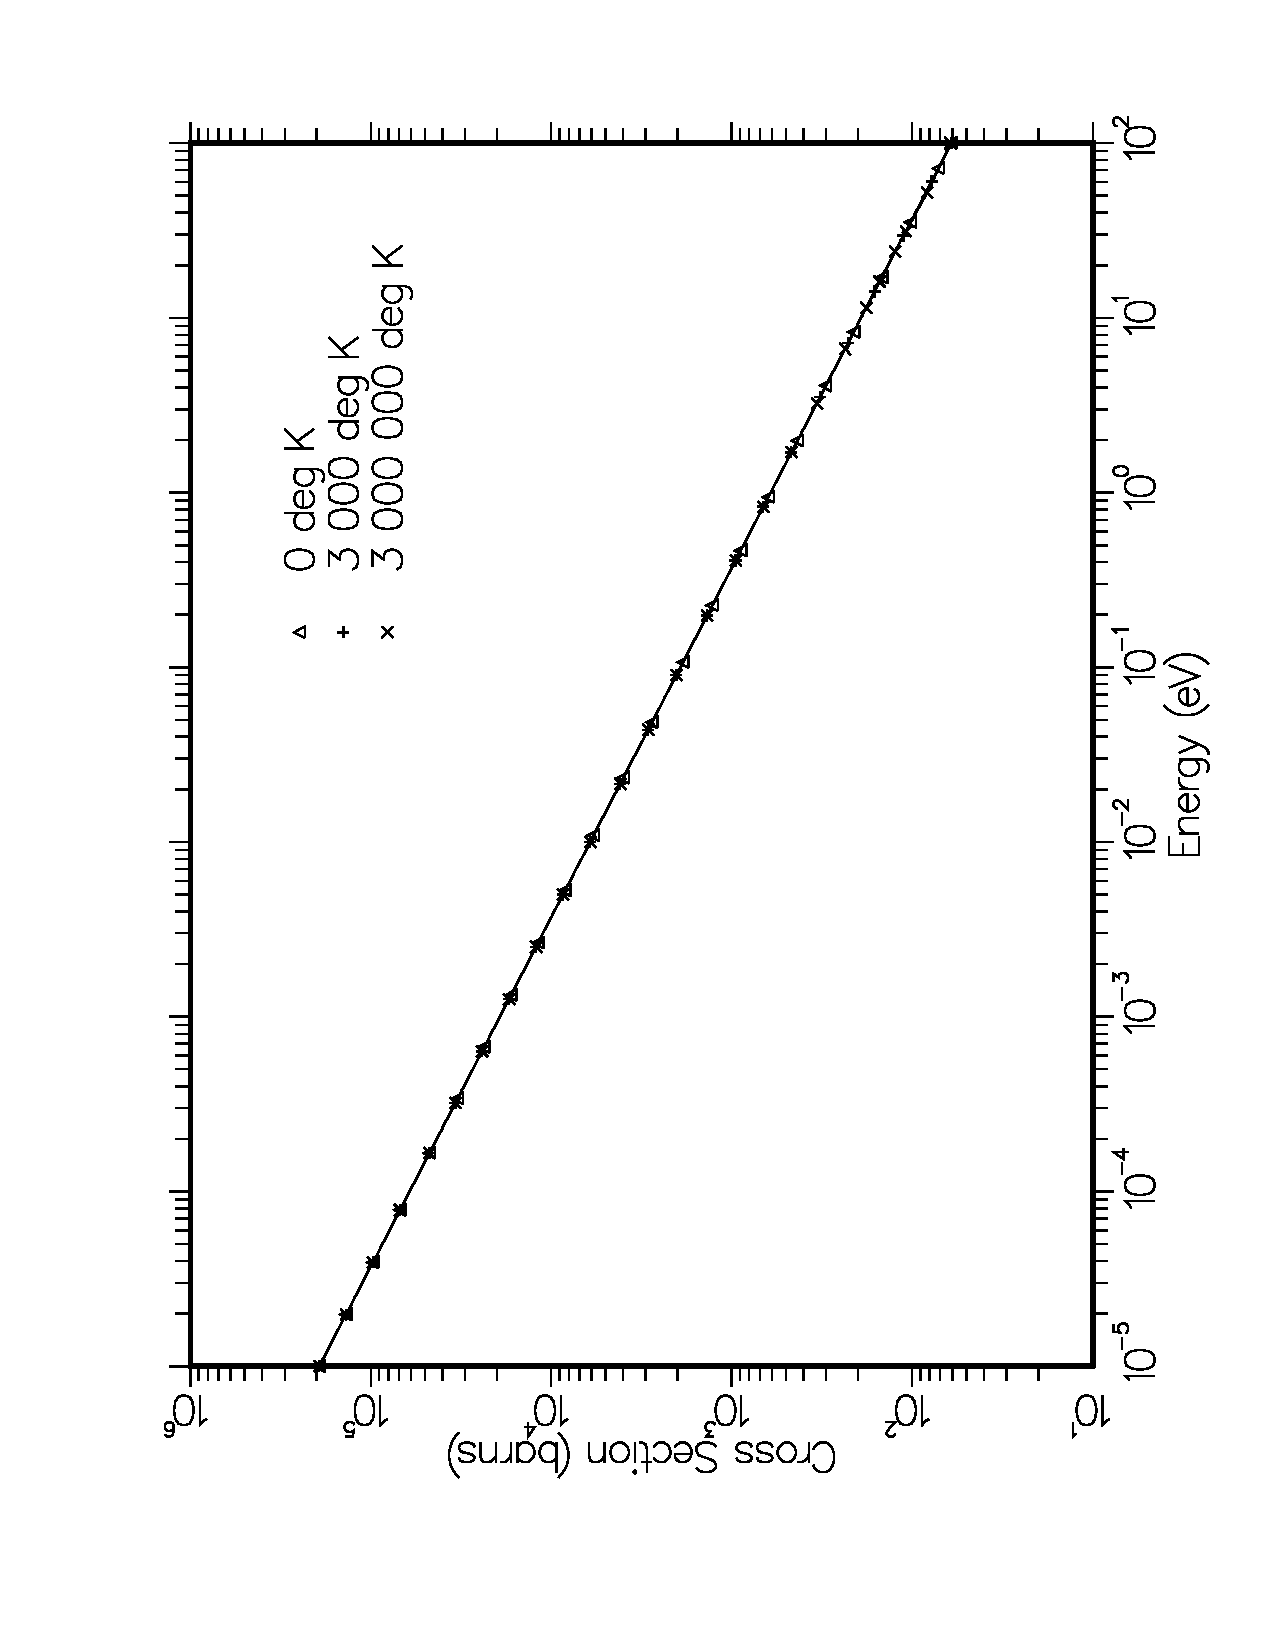
\includegraphics[keepaspectratio, height=4.0in, angle=270]{figs/broadr1ack}
\caption[The $^{10}$B (n,$\alpha$) cross section versus Doppler broadening
temperature]
{The (n,$\alpha$) cross section for $^{10}$B
        from ENDF/B-V for three different temperatures showing that
        a $1/v$ cross section is invariant under Doppler-broadening.}
\label{over}
\end{figure}

When interpreting BROADR output, it is useful to remember several
important features of the Doppler-broadening process.
\index{Doppler-broadening}
A $1/v$ cross section remains unchanged.  Contrary to ``popular
knowledge'', the area under a resonance does not remain unchanged
unless $E\gg kT/A$.  In fact, each resonance develops a new $1/v$
tail.  Finally, a constant cross section (for example, elastic
scattering) develops a $1/v$ tail at low energies after
Doppler-broadening.  These effects are shown in Figs.~\ref{over},
\ref{elas}, and \ref{reson};  they can be best understood by noting
that the Doppler process preserves reaction rate $v\sigma (v)$
according to Eq.~(\ref{effxs}), and a finite reaction rate is
expected for $T>0$K even as $v\rightarrow 0$.

\begin{figure}[thbp]\centering
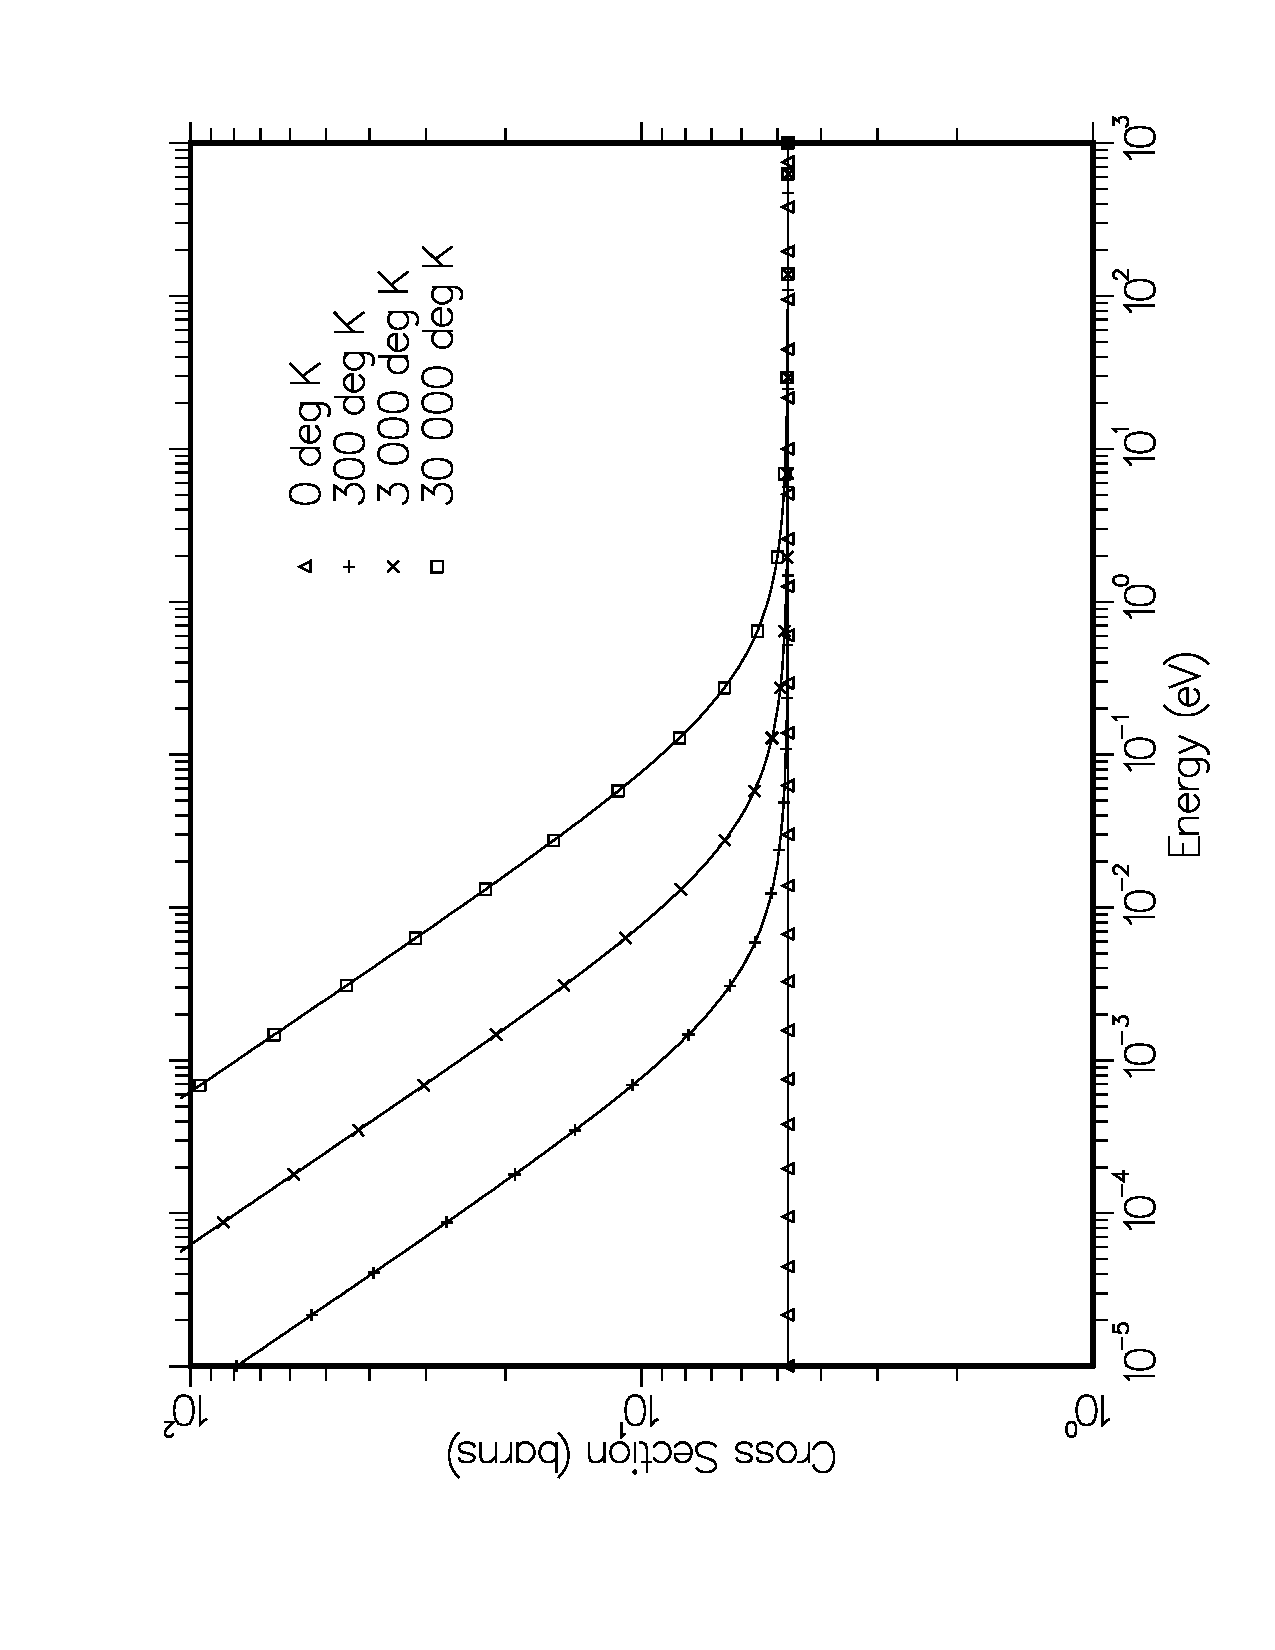
\includegraphics[height=4.0in, angle=270]{figs/broadr2ack}
\caption[The $^{nat}$C elastic scattering cross section versus Doppler
 broadening temperature]
{The elastic cross section for carbon
        from ENDF/B-V showing that Doppler-broadening a constant
        cross section adds a $1/v$ tail.}
\label{elas}
\end{figure}

\begin{figure}[thbp]\centering
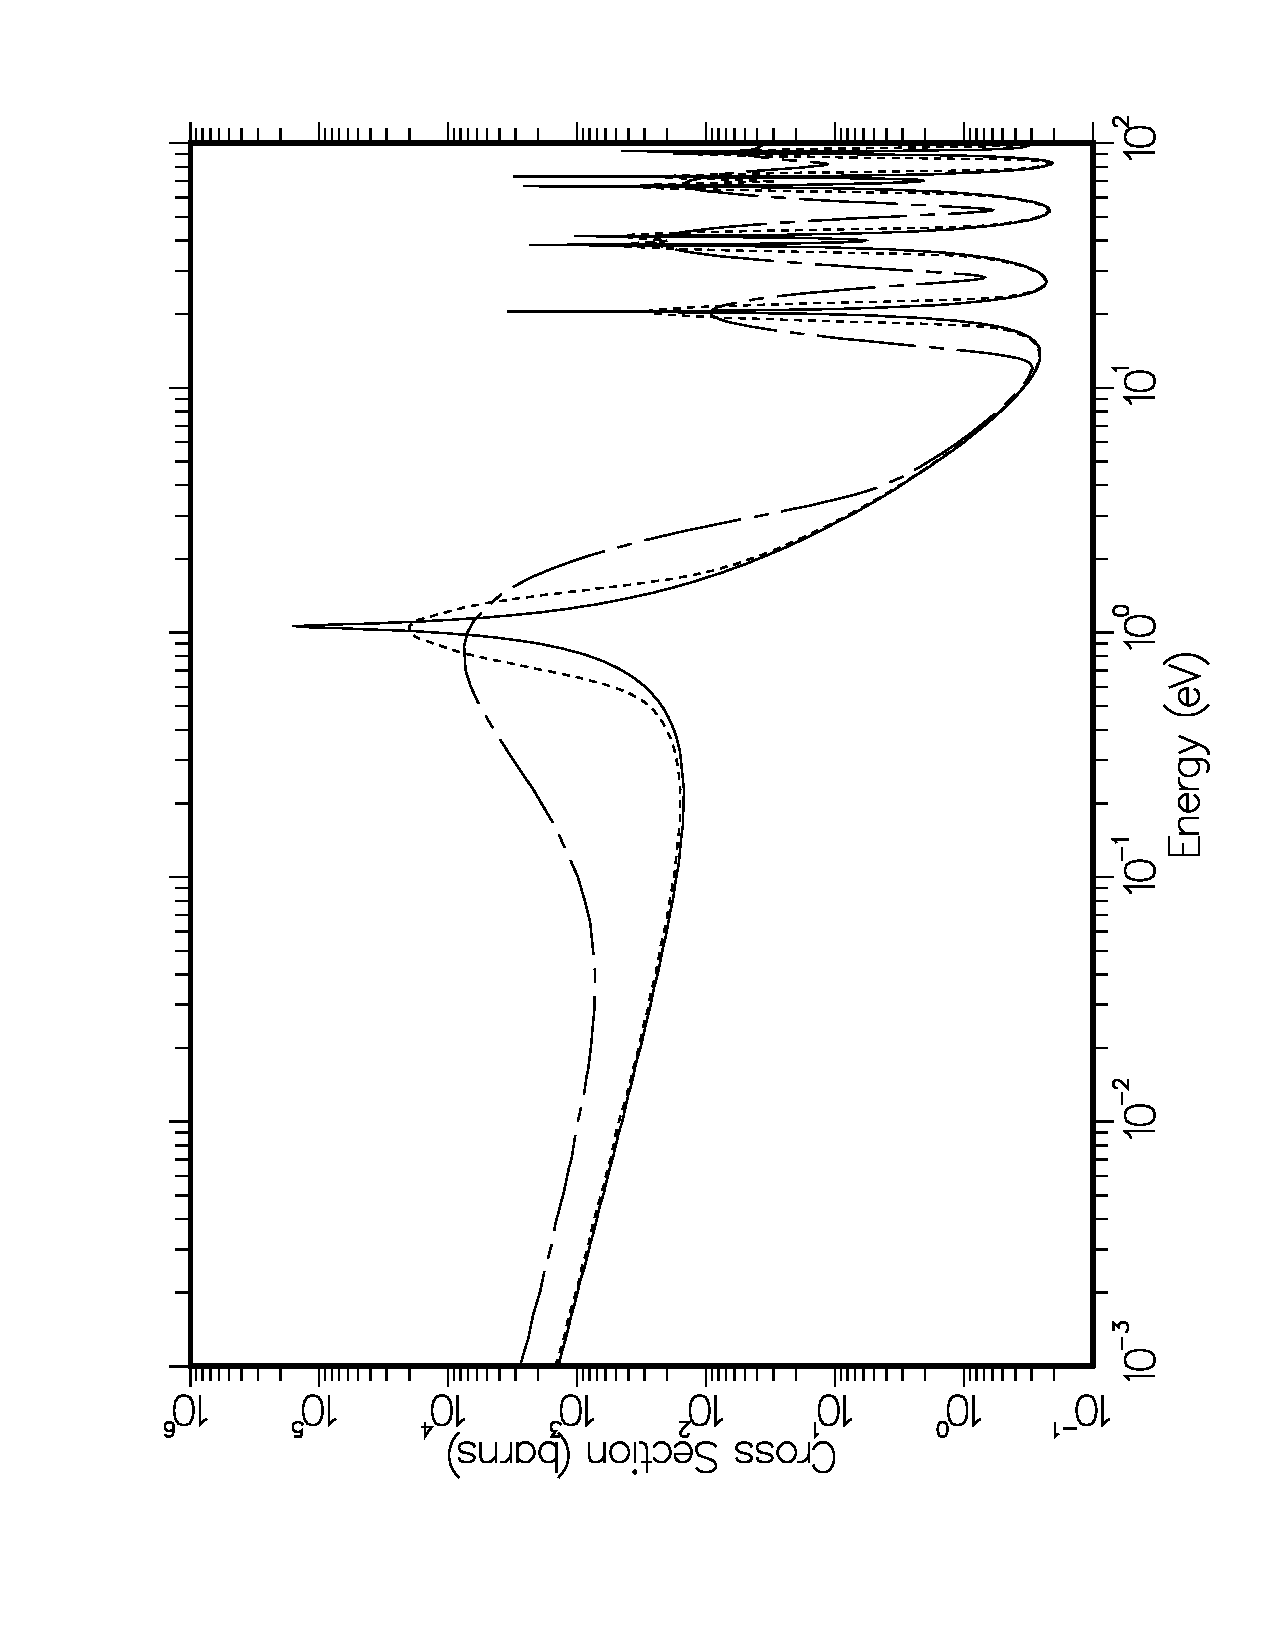
\includegraphics[keepaspectratio, height=3.6in, angle=270]{figs/broadr3ack}
\caption[The $^{240}$Pu low energy (n,$\gamma$) cross section versus Doppler
 broadening temperature]
{The (n,$\gamma$) cross section for
 $^{240}$Pu for several temperatures showing
 the effects of Doppler broadening on resonances.  The
 temperatures are 0K (solid), 30\ 000K (dotted), and
 300\ 000K (dash-dot).  The higher resonances behave in
 the classical manner even at 30\ 000K; note that the
 line shape returns to the asymptotic value in the wings
 of the resonance.  All resonances at 300\ 000K (and to a
 lesser extent the first resonance for 30\ 000K) show the
 additional $1/v$ component that appears when $kT/A$ is
 large with respect to the resonance energy.}
   \label{reson}
\end{figure}

Very early (1980s) versions of BROADR and SIGMA1 assumed that the input
energy grid from \hyperlink{sRECONRhy}{RECONR}\index{RECONR}
could also be used to represent
the Doppler-broadened cross section before thinning.  The grid was
then thinned to take advantage of the smoothing effect of Doppler
broadening.  Unfortunately, this assumption is inadequate.  The
reconstruction process in \hyperlink{sRECONRhy}{RECONR} places many points
near the center of a resonance to represent its sharp sides.  After
broadening, the cross section in this energy region becomes
rather smooth;  the sharp sides are moved out to energies where
\hyperlink{sRECONRhy}{RECONR} provides few points.  At still higher energies,
the resonance line shape returns to its asymptotic value, and the
\hyperlink{sRECONRhy}{RECONR} grid is adequate once more.  The more recent
versions of BROADR check the cross section between points of the incoming
energy grid, and add additional grid points if they are necessary
to represent the broadened line shape to the desired accuracy.
This effect is illustrated in Fig.~\ref{grids}.

\begin{figure}[t]\centering
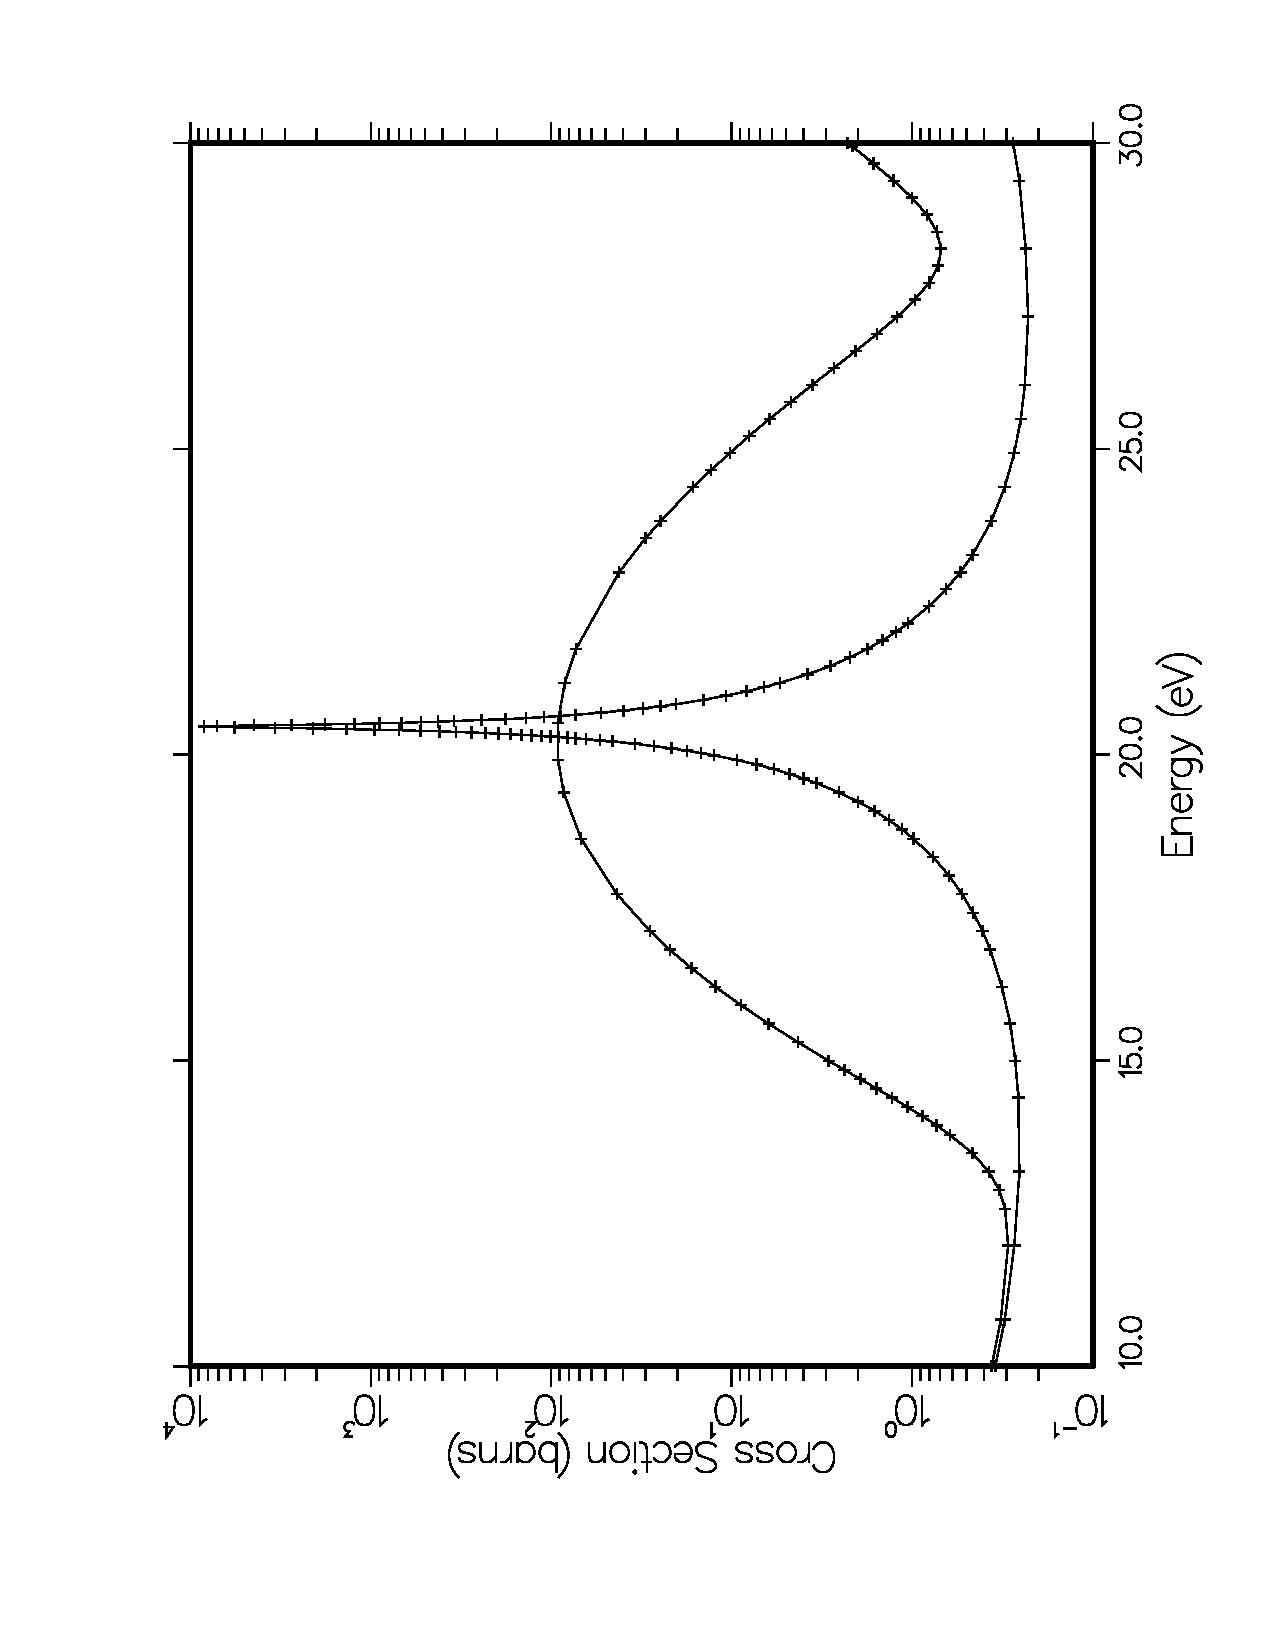
\includegraphics[keepaspectratio, height=3.6in, angle=270]{figs/broadr4ack}
\caption[Energy grid variation with Doppler broadening]{An expanded plot
 of the 20 eV resonance  from Fig.~\ref{reson} showing both thinning
 and ``thickening'' of the energy grid produced adaptively
 by BROADR.  The two curves show the capture cross section
 at 0K and 300 000K.  Note that the high-temperature
 curve has fewer points than the 0K curve near the peak
 at 20 eV and more  points in the wings near 15 eV and 25
 eV.  Clearly, using the 0K grid to represent the
 broadened cross section in the wings of this resonance
 would give poor results.}
   \label{grids}
\end{figure}

\subsection{Thermal Quantities}
\label{ssBROADR_thermal}

In thermal-reactor work, people make very effective use of a few
standard thermal constants\index{thermal constants} to
characterize nuclear systems.  These parameters include
the cross sections at the standard thermal value of
0.0253 eV (2200 m/s), the integrals of the cross sections
against a Maxwellian distribution for 0.0253 eV, the g-factors
(which express the ratio between a Maxwellian integral and the
corresponding thermal cross section), $\eta$, $\alpha$, and K1.
Here, $\eta$ is the Maxwellian-weighted average of
$(\bar{\nu)}\sigma_f)/(\sigma_f+\sigma_c)$, $\alpha$ is
the average of $\sigma_c/\sigma_f$, and K1 is the average
of $(\bar{\nu}-1)\sigma_f-\sigma_c$.  If BROADR is run for a
temperature close to 293.6K (which is equivalent to 0.0253 eV),
these thermal quantities are automatically calculated and displayed.
Here is a sample output for $^{235}$U from ENDF/B-VII\index{ENDF!ENDF/B-VII}:

\small
\begin{ccode}

    thermal quantities at 293.6 K = 0.0253 eV
    -----------------------------------------
           thermal fission xsec:  5.8490E+02
          thermal fission nubar:  2.4367E+00
           thermal capture xsec:  9.8665E+01
       thermal capture g-factor:  9.9086E-01
       thermal capture integral:  8.6639E+01
     capture resonance integral:  1.4043E+02
       thermal fission integral:  5.0605E+02
       thermal fission g-factor:  9.7628E-01
         thermal alpha integral:  1.6828E-01
           thermal eta integral:  2.0859E+00
            thermal k1 integral:  6.4040E+02
                  equivalent k1:  7.2262E+02
     fission resonance integral:  2.7596E+02
    -----------------------------------------

\end{ccode}
\normalsize

\subsection{Data-Paging Methodology}
\label{ssBROADR_paging}

A piecewise linear representation of a reaction cross section of
a resonance material may require a very large number of energy
points.  For example, ENDF/B-VII $^{238}$U (MAT9237) requires 167\ 000
points for the total cross section for 0.1\% precision
(\cword{errmax}=\cword{err}).  It is impractical to load all these points
into memory simultaneously.  However, the discussion following
Eq.~(\ref{sigv}) in the theory section shows that only a limited
energy range around the point of interest is required.

The strategy used is to stage the cross-section data into three
``pages'' of \cword{npage} points each.\index{paging}  Points in
the center page can then be broadened using the \cword{npage} or
more points on each side of the point of interest.  If
$v-4/\sqrt{\alpha}$ and $v+4/\sqrt{\alpha}$ are both included in
the three-page range, accurate broadening can be performed.  If
not, a diagnostic warning is printed; the user should repeat the
calculation with a smaller temperature step or a larger page
size.

There are many different reaction cross sections for each
material.  However, the cross sections for high velocities are
normally smooth with respect to $32kT/A$ for any temperatures
outside of stellar photospheres; therefore, they do not show
significant Doppler effects.  Until recently the upper energy limit
for Doppler broadening was the smallest of (i) the input value
\cword{thnmax}, (ii) the upper limit of the resolved-resonance
energy range, (iii) the lowest threshold, or (iv) 1.0 MeV
(the default input value for \cword{thnmax}).  No Doppler
broadening or energy-grid reconstruction is performed
above that energy.  In the past, and what users
typically expect as the default action, the second condition
often set the Doppler broadening upper limit.

However recent evaluated files have increasingly included threshold
reactions at energies within the resolved resonance energy
range.  For example, recent JENDL evaluations for $^{235}$U include a
resolved-resonance range upper limit of 2.25 keV, but also
include non-zero cross sections for an inelastic level with a 77 eV
threshold.  Under the rules itemized above, Doppler broadening of
these data stops at 77 eV.  Other evaluations ({\it e.g.}, ENDF/B-VI,
ENDF/B-VII and JEFF-3.1) share the same resolved-resonance range data but
have zeroed out this inelastic cross section from 77 eV to 2.25 keV
and so Doppler broadening of these files occurs throughout the
resolved-resonance range, as most users expect.

Zeroing out non-zero data is a cludge from the past and so we have
changed the Doppler upper energy limit logic so that the top of the
resolved resonance range is now the default condition.  This means
that non-threshold reactions are also Doppler broadened.  The
mathematics of this operation can produce non-zero cross sections
at energies below the reaction threshold.  If this occurs those
cross sections are zeroed.

As noted in the BROADR module source code comments, users
may specify a negative value for \cword{thnmax} to override these
selection rules and force Doppler broadening to an upper energy
of \cword{abs(thnmax)} eV.  This has been a long-term NJOY feature
that remains unchanged in NJOY2016.

Finally, we note that the $A_i$ and $B_i$
factors in Eq.~(\ref{sigy}) depend only on the energy (or
velocity) values and not on the cross sections.  Since the $A_i$
and $B_i$ are expensive to compute, the code computes them only
once for the points of a unionized energy grid.  The sum of
Eq.~(\ref{sigy}) is accumulated for all the non-threshold
reactions simultaneously.  This feature helps make BROADR run
faster.

\subsection{Coding Details}
\label{ssBROADR_details}

The main subroutine for BROADR is
\cword{broadr}\index{broadr@{\ty broadr}} from
module \cword{broadm}\index{modules!broadm@{\ty broadm}}.  The
code begins by reading the user's input (see Section~\ref{ssBROADR_inp}).
Storage is then allocated for the \cword{loada/finda} buffers
(\cword{ibufo} and \cword{ibufn}) and for the scratch storage
(\cword{iscr}).  The buffer length \cword{nbuf} can be changed at
will (currently \cword{nbuf} is 1000).

The input PENDF\index{PENDF} tape is searched for the desired material
(\cword{mat1}).  If the restart option is set (\cword{istart}=1),
the temperatures less than or equal to \cword{temp1} for
\cword{mat1} are assumed to have been broadened previously, and
they are copied to the output file.  In either case, the files
for \cword{temp1} are copied to a scratch file on unit
\cword{nscr1}.

Next, \cword{nscr1} is rewound and examined reaction by
reaction.  The energy grid from the total cross section (MT1) is
saved on scratch storage using \cword{loada}.  If the input tape
has not been through \hyperlink{sRECONRhy}{RECONR}\index{RECONR},
the BROADR module will
still run, but at possibly reduced accuracy.  The next low-threshold
reaction (that is, the next reaction with a threshold less than
\cword{emin}, which is currently 1 eV) is located on
\cword{nscr1}.  The energy points are retrieved from scratch file
\cword{iold} (12 or 13) using \cword{finda}, the cross sections
for this reaction are computed on this grid, and the results are
stored on scratch file \cword{inew} (13 or 12) using
\cword{loada}.  The units for \cword{iold} and \cword{inew} are
then exchanged, and the entire process is repeated for the next
low-threshold reaction.

The final result of this process is a list of \cword{nreac}
low-threshold-reaction types in \cword{mtr} (usually MT2, MT18,
and MT102), the threshold value for the first high-threshold
reaction (or the input value) in \cword{thnmax}, and scratch file
\cword{iold} containing the energy grid and all the low-threshold
reactions (there are \cword{n2in} points).

Now that the number of reactions to be broadened simultaneously
is known (\cword{nreac}), storage for data paging can be assigned.
The total amount of storage available is \cword{namax}.  The value
of \cword{namax} should be as large as possible (current value
is 15\ 000\ 000).  This space is divided up into the largest possible
page size, \cword{npage}.  An overflow region \cword{nstack} is also
allocated.  Now that the page size is known, the code allocates three
pages for energies (\cword{e}), three pages for each reaction
cross section (\cword{s}), one extended page for the broadened
energy grid (\cword{eb}), and three extended pages for the
broadened cross section (\cword{sb}).  This system is designed to
use the available storage with maximum efficiency.

The cross sections on \cword{iold} are now broadened by
\cword{bfile3}\index{bfile3@{\ty bfile3}} (see below) and the results
are written on scratch unit \cword{inew} using \cword{loada}.

The directory from \cword{nscr1} is revised to reflect any thinning
or thickening and written on the output PENDF tape (\cword{nout}).
Note that the new temperature is written into the first word of the
Hollerith data record to simplify later searching.

The broadened cross sections are now converted into ENDF TAB1
\index{TAB1@{\ty TAB1}} records and merged with the unbroadened
cross sections on \cword{nscr1}.  The total cross section (and
sometimes nonelastic, inelastic, fission, (n,2n), or
charged-particle reactions) is reconstructed to equal the
sum of its parts\index{summation cross sections}.  The new
Doppler-broadened ``MAT'' on \cword{NOUT} is a legal PENDF file
with the same MAT number as the original data but with a
new temperature.

The process is now repeated for each of the \cword{ntemp2} final
temperatures \cword{temp2} requested.  Note that after each step
\cword{inew} contains the new data and \cword{iold} contains the
previous data.  If the ``bootstrap'' option is set
(\cword{istrap}=1), these units are interchanged.  For this
option, \cword{stemp2(it)} is always obtained from
\cword{temp2(it-1)}.  Because of the thinning effect of
Doppler-broadening, the broadening runs faster at each step.  The
accumulation of error is usually not a problem.  For
\cword{istrap}=0, \cword{temp1} is used for the starting
temperature every time.

The broadening and energy-grid reconstruction are directed by
\cword{bfile3}\index{bfile3@{\ty bfile3}} .  The routine loads data
into the appropriate memory pages from scratch file \cword{iold} and
then either calls \cword{broadn}\index{broadn@{\ty broadn}}
to broaden it (with thinning or thickening of the grid as necessary)
or calls \cword{thinb}\index{thinb@{\ty thinb}} to thin
it without broadening.  The results are written onto scratch file
\cword{inew}.

In \cword{broadn}\index{broadn@{\ty broadn}}, the energy grid points
just loaded into \cword{e} by \cword{bfile3}\index{bfile3@{\ty bfile3}}
are converted to the dimensionless variables x and y
[see Eq.~(\ref{sigmax})].  An adaptive reconstruction
\index{adaptive reconstruction} of the Doppler broadened
cross section is then performed for the energy range in the
center page using an inverted stack\index{inverted stack}
algorithm like the one described for
\hyperlink{sRECONRhy}{RECONR}\index{RECONR}.  The
upper limit of each panel is taken to be a point from the input
grid, but in order to allow for thinning, up to \cword{nmax}=10
of the input grid points can be skipped before the actual upper
limit is selected.  In addition, the energy of the upper limit
cannot be more than \cword{step}=2.01 times the energy of the
preceding point.  The cross sections are now computed at the
midpoint of the top panel in the stack using \cword{bsigma}.  If
the results differ from the values obtained by interpolation by
more than the specified tolerance, the new point is added to the
stack, and the tests are repeated.  Otherwise, the top point in
the stack is converged.  A backward check is made to see if some
of the previous points can be removed based on the new value, the
new value is stored in the output array, and the height of the
stack is reduced by one.   The routine now tries to subdivide the
new panel at the top of the stack in the same way.  When the
stack has been reduced to one element, a new upper limit is
chosen from the input energy grid as described above, and the
entire process is repeated.  The reconstruction logic in BROADR
uses the same integral tests as
\hyperlink{sRECONRhy}{RECONR}\index{RECONR}.  Refer to
the \hyperlink{sRECONRhy}{RECONR} chapter for more details.

Subroutine \cword{bsigma}\index{bsigma@{\ty bsigma}} is used
to calculate the actual broadened cross section at an energy
point using the data in the three pages.  First, the routine
locates the energy panel containing the desired energy \cword{en}.
It then loops over intervals below the current point adding in
contributions to $\bar{\sigma}$ from the $V{-}v$ term of
Eq.~(\ref{standform}) until the contributions to the cross section
become small.  If the lower limit of the bottom page is reached
before convergence, a warning message is issued.  The routine
then loops over intervals above the current point until
convergence.  Once again, a warning is issued if necessary.
Finally, the low-energy term [the one involving
$V{+}v$ in Eq.~(\ref{standform})] is added, if applicable.

Subroutine \cword{thinb}\index{thinb@{\ty thinb}} is provided
for cases where the input cross section set is to be thinned only.
 This routine uses the original SIGMA1\index{SIGMA1} method.  The
first input point is always kept.  The routine then loops over
higher energy values.  For each grid point, all the points from
there back to the last accepted point are checked for their
deviation from a straight line.  If they all can be removed
without violating the specified tolerance, the interval is
extended to the next higher point and the tests are
repeated.  If any point in the range is too far from the linear
approximation, the last point in the range is accepted as an
output point, and the testing process is repeated starting from
this new lower limit.  The procedure terminates when all of the
points in the middle page have been thinned, and control is
returned to \cword{bfile3}\index{bfile3@{\ty bfile3}} to get
the next page of data.  Thinning may have been a necessary
feature in the past when computing resources were limited but
is a rarely used feature today.

Subroutine \cword{hunky}\index{hunky@{\ty hunky}} has been modified
from the original SIGMA1 version to implement the alternate
$H_n(a,b)$ calculation when necessary (see
\cword{hnabb}\index{hnabb@{\ty hnabb}}).  When using the direct
method, $F_n$ values from the previous step are used in the
difference of Eq.~(\ref{diffs}), and \cword{funky} is called to
get the new values.  The $A_i$ and $B_i$ of Eq.~(\ref{sigy}) are
related to the \cword{s1} and \cword{s2} here.

Subroutine \cword{funky}\index{funky@{\ty funky}} evaluates
$F_n(a)$ by the recursion formula of Eq.~(\ref{recur}) using
the very accurate SLATEC\index{SLATEC} version of
the reduced complementary error function
\index{complementary error function} from the NJOY2016
math module\index{modules!math@{\ty math}}.

Function \cword{hnabb}\index{hnabb@{\ty hnabb}} implements the
alternate calculation described by Eqs.~(\ref{alt1})-(\ref{alt2}).
The series expansion is continued until about six significant figures
are guaranteed (see \cword{eps} and \cword{hnabb}).  Currently,
\cword{hnabb} is called when only four significant figures are
reliable in \cword{hunky} (see \cword{toler} in \cword{hunky}).

\subsection{User Input}
\label{ssBROADR_inp}

The following input instructions have been copied from the
comment cards at the start of BROADR.
\index{BROADR!BROADR input}
\index{input!BROADR}

\small
\begin{ccode}

   !---input specifications (free format)---------------------------
   !
   ! card 1
   !    nendf    input endf tape (for thermal nubar only)
   !    nin      input pendf tape
   !    nout     output pendf tape
   !
   ! card 2
   !    mat1     material to broadened and thinned
   !    ntemp2   number of final temperatures (default=1)
   !    istart   restart (0 no, 1 yes, default 0)
   !    istrap   bootstrap (0 no, 1 yes, default 0
   !    temp1    starting temperature from nin (default=0K)
   !
   ! card 3
   !    errthn   fractional tolerance for thinning
   !    thnmax   max. energy for broadening and thinning
   !             (default=1 MeV)
   !    errmax   fractional tolerance used when integral criterion
   !             is satisfied (same usage as in reconr)
   !             (errmax.ge.errthn, default=10*errthn)
   !    errint   parameter to control integral thinning
   !             (usage as in reconr) (default=errthn/20000)
   !             set very small to turn off integral thinning.
   !      (A good choice for the convergence parameters
   !       errthn, errmax, and errint is the same set of
   !       values used in reconr)
   !
   ! card 4
   !    temp2    final temperatures (deg Kelvin)
   !
   ! card 5
   !    mat1     next MAT number to be processed with these
   !             parameters.  Terminate with mat1=0.
   !
   !---input options------------------------------------------------
   !
   ! The output tape will contain the ntemp2 final temperatures
   ! specified.  It is necessary to have temp1.le.temp2(1).
   ! if temp2.eq.temp1, the data will be thinned only.
   !
   ! restart    Continue broadening an existing pendf tape.  All
   !            temperatures are copied through temp1.  Additional
   !            final temperatures are added by starting with the
   !            data at temp1.
   !
   ! bootstrap  If bootstrap is not requested, each final tempera-
   !            ture is generated by broadening directly from temp1
   !            to temp2.  If bootstrap is requested, each final temp-
   !            erature is broadened from the preceding temperature.
   !            Bootstrapping is faster due to the thinning in the
   !            previous step.  However, errors accumulate.
   !
   ! thnmax     A possible upper limit for broadening and thinning.
   !            The actual upper limit is the lowest of (i) this input
   !            value; (ii) the end of the resolved resonance range;
   !            (iii) the lowest reaction threshold; or (iv) 1.0 MeV.
   !
   !            A negative value for thnmax forces the Doppler
   !            broadening upper limit to be abs(thnmax) irrespective
   !            of the other conditions.
   !
   !            Caution:  this may cause one or more threshold
   !            reactions to be broadened.  The magnitude of
   !            thnmax must be chosen to keep the number of
   !            broadenable reactions less than or equal to the
   !            maximum of ntt (160).
   !
   !            Caution: for use in transport codes, it is recommended
   !            to use the program default.  We don't know how
   !            to compute the spectrum of scattered neutrons from
   !            a broadened inelastic level in the current generation
   !            of codes.  Broadened cross sections for threshold
   !            reactions may be useful for other purposes.
   !
   !-------------------------------------------------------------------

\end{ccode}
\normalsize

Note that \cword{temp1} need not occur on \cword{nout} if
\cword{istart}=0.  The restart\index{restart} option
(\cword{istart}=1) enables the user to add new temperatures
to the end of an existing PENDF\index{PENDF} tape.  This
option is also useful if a job runs out of time while
processing, for example, the fifth temperature in a job requesting
six or more final temperatures.  The job can be
restarted from the \cword{nout}.  The first four temperatures
will be copied to the new \cword{nout} and broadening will
continue for temperature five.  The bootstrap\index{bootstrap}
option speeds up the code by using the broadened result for
\cword{temp2(i-1)} as the starting point to obtain \cword{temp2(i)}.
The \cword{thnmax} parameters can be used to speed up a calculation
or to prevent the broadening of inappropriate data such as sharp
steps or triangles in an evaluated cross section (for example,
ENDF/B-V lead).

The following example prepares a broadened PENDF file for
$^{235}$U from ENDF/B-VII\index{ENDF!ENDF/B-VII} at two temperatures.
The line numbers are for reference only; they are not part
of the input.
\small
\begin{ccode}

   1.  broadr
   2.  20 21 22/
   3.  9228 2/
   4.  .001/
   5.  300. 1200./
   6.  0/

\end{ccode}
\normalsize

\noindent   On line 2, unit 20 should contain the ENDF file and
unit 21 should a \hyperlink{sRECONRhy}{RECONR}-generated ASCII
PENDF file of 0K cross sections for the
isotope.  Two materials will be generated on unit 21 with 0.1\%
accuracy.  First will be the 300K data, followed by a MEND record,
followed by the 1200K data, followed by MEND and and TEND records.
Best results are obtained when the error tolerance \cword{errthn}
and the optional integral-thinning controls \cword{errmax}
and \cword{errint} are the same as those used for the
\hyperlink{sRECONRhy}{RECONR}\index{RECONR} run.

\subsection{Error Messages}
\label{ssCROADR_msg}

\begin{description}
\begin{singlespace}

\item[\cword{error in broadr***nin and nout must be same mode}] ~\par
  Use coded to coded, or blocked binary to blocked binary.
  The latter is faster due to the several tape copies
  performed in BROADR.

\item[\cword{error in broadr***max. energy too large ...}] ~\par
  The user requested Doppler broadening to an energy beyond
the maximum energy in the ENDF file.

\item[\cword{error in broadr***too many low threshold reactions}] ~\par
  The current limit is set by the global parameter \cword{ntt}=180.
  Check \cword{tt}, \cword{mtr}, and \cword{ntt} in \cword{broadr},
  \cword{tt} in \cword{bfile3}, and \cword{sbt} in \cword{broadn}.

\item[\cword{message from broadr---desired mat and temp not on tape}] ~\par
  Check the input PENDF file and the user input.

\item[\cword{message from broadr---no broadenable reactions}] ~\par
  No low threshold reactions were found.

\item[\cword{error in broadr***storage exceeded}] ~\par
  Insufficient storage to update directory.  Increase
  \cword{nwscr}=1000 in \cword{broadr}.

\item[\cword{message from stounx---sigma zero data removed ...}] ~\par
  The input PENDF tape already contained a special unresolved section
  in File 2.  It has been removed.  Rerun \hyperlink{sUNRESRhy}{UNRESR}
  if necessary.

\item[\cword{message from bsigma---broadening truncated at a=----}] ~\par
  The page is too small for the temperature difference
  requested.  Increase total storage available (\cword{namax}) or repeat
  the calculation with smaller temperature steps and
  \cword{istrap}=1.  The normal maximum size of \cword{a}
  is 4.0 and \cword{a} is inversely proportional to $T_i{-}T_{i-1}$.

\end{singlespace}
\end{description}

\subsection{Input/Output Units}
\label{ssBROADR_IOunits}

The following units are used for input and output by BROADR.
\begin{list}{}{\leftmargin=.75in\labelsep=.25in\labelwidth=.5in}
\begin{singlespace}

\item[10]    \cword{nscr1} in BROADR.  Contains the ENDF/B data at the
             initial temperature.
\item[12/13] \cword{iold/inew} in BROADR.  Contains union grid and
             low threshold reactions.
\item[20-99] User's choice for \cword{nin} and \cword{nout} to link with
             other modules.

\end{singlespace}
\end{list}

\noindent
Units 12 and 13 will always be binary.  Unit 10 will have the
same mode as \cword{nin} and \cword{nout}.

\subsection{Storage Allocation}
\label{ssBROADR_storage}

All storage is divided in the most efficient way possible.  The
container array size \cword{namax} should be made as large as possible.
The value of \cword{nbuf} can be increased or decreased at will --- larger
values will give faster execution.  The value for \cword{nwscr} depends
on the size of the ENDF/B dictionary, and 1000 words is sufficient for
all current evaluations.

\cleardoublepage


\section{UNRESR}
\label{sUNRESR}

\hypertarget{sUNRESRhy}{The}
UNRESR\index{UNRESR|textbf} module is used to produce effective self-shielded
\index{self-shielding} cross sections for resonance reactions in the
unresolved energy range.\index{unresolved resonance range} In ENDF-format
evaluations, the unresolved range begins at an energy where it is difficult
to measure individual resonances and extends to an energy where the effects
of fluctuations in the resonance cross sections become unimportant for
practical calculations.  As described in the ENDF format
manual,\cite{ENDF102} resonance information for this energy range is
given as average values for resonance widths and spacings together
with distribution functions for the widths and spacings.  This
representation can be converted into effective cross sections suitable
for codes that use the background cross section method, often
called the Bondarenko method,\cite{Bondarenko}\index{Bondarenko method}
using a method originally developed for the MC2
code\cite{MC2}\index{MC2} and extended for the ETOX
code\cite{ETOX}\index{ETOX}.  This unresolved-resonance method
has the following features:

\begin{itemize}
\begin{singlespace}
\item Flux-weighted cross sections are produced for the total,
    elastic, fission, and capture cross sections, including
    competition with inelastic scattering.

\item A current-weighted total cross section is produced for
    calculating the effective self-shielded transport cross section.

\item The energy grid used is consistent with the grid used by
   \hyperlink{sRECONRhy}{RECONR}.

\item The computed effective cross sections are written on the
   PENDF tape in a specially defined section (MF2, MT152) for
   use by other modules.

\item The accurate quadrature scheme from the MC2-2 code\cite{MC22}
   is used for computing averages over the ENDF statistical distribution
   functions.
\end{singlespace}
\end{itemize}

This chapter describes the UNRESR module in NJOY2016.0.

\subsection{Theory}
\label{ssUNRESR_theory}

In the unresolved energy range, it is not possible to define
precise values for the cross sections of the resonance reactions
$\sigma_x(E)$, where $x$ stands for the reaction type (total,
elastic, fission, or capture).  It is only possible to define
average values.  Of course, these average values should try
to preserve the reaction rate:

\begin{equation}
   \overline{\sigma}_{0x}(E^*)=\frac
     {\displaystyle\int_{E_1}^{E_2}\sigma_x(E)\,\phi_0(E)\,dE}
     {\displaystyle\int_{E_1}^{E_2}\phi_0(E)\,dE}\,\,,
\label{sbar0}
\end{equation}

\noindent
where $\phi_0(E)$ is the scalar flux, $E^*$ is an effective energy
in the range $[E_1,E_2]$, and the range $[E_1,E_2]$ is large
enough to hold many resonances but small with respect to
slowly varying functions of $E$.  In order to calculate
effective values for the transport cross section, it is
necessary to compute the current-weighted total cross
\index{current weighting}
section also.  It is given by

\begin{equation}
   \overline{\sigma}_{1t}(E^*)=\frac
     {\displaystyle\int_{E_1}^{E_2}\sigma_x(E)\,\phi_1(E)\,dE}
     {\displaystyle\int_{E_1}^{E_2}\phi_1(E)\,dE}\,\,,
\end{equation}

\noindent
where the P$_1$ component of the neutron flux, $\phi_1(E)$, is
proportional to the neutron current.  To proceed farther, it is
necessary to choose a model for the shape of $\phi_\ell(E)$ in the
vicinity of $E^*$.  The model used in UNRESR is based on the
B$_0$ approximation for large homogeneous systems and narrow
resonances:

\begin{equation}
   \phi_\ell(E)=\frac{C(E)}{[\,\Sigma_t(E)\,]^\ell}\,\,,
\end{equation}

\noindent
where $C(E)$ is a slowly varying function of $E$, and
$\Sigma_t(E)$ is the macroscopic total cross
section for the system.  In order to use this result in
Eq.~\ref{sbar0}, it is further assumed that the effects of other
isotopes in the mixture can be approximated by a constant called
$\sigma_0$ in the range $[E_1,E_2]$, or

\begin{equation}
   \phi_\ell(E)=\frac{C(E)}{[\,\sigma_0+\sigma_t(E)\,]^\ell}\,\,.
\label{flux}
\end{equation}

\noindent
Therefore, the effective cross sections in the unresolved range
are represented by

\begin{equation}
   \overline{\sigma}_{0x}(E^*)=\displaystyle\frac
     {\displaystyle\int_{E_1}^{E_2}
        \frac{\sigma_x(E)}{\sigma_0+\sigma_t(E)}C(E)\,dE}
     {\displaystyle\int_{E_1}^{E_2}
        \frac{1}{\sigma_0+\sigma_t(E)}C(E)\,dE}\,\,,
\end{equation}

\noindent
with $x$ being $t$ for total, $e$ for elastic, $f$ for fission,
and $\gamma$ for capture, and

\begin{equation}
   \overline{\sigma}_{1t}(E^*)=\displaystyle\frac
     {\displaystyle\int_{E_1}^{E_2}
        \frac{\sigma_x(E)}{[\,\sigma_0+\sigma_t(E)\,]^2}C(E)\,dE}
     {\displaystyle\int_{E_1}^{E_2}
        \frac{1}{[\,\sigma_0+\sigma_t(E)\,]^2}C(E)\,dE}\,\,.
\end{equation}

\noindent
This equation can also be written in the equivalent form

\begin{equation}
   \overline{\sigma}_{1t}(E^*)=\displaystyle\frac
     {\displaystyle\int_{E_1}^{E_2}
        \frac{1}{\sigma_0+\sigma_t(E)}C(E)\,dE}
     {\displaystyle\int_{E_1}^{E_2}
        \frac{1}{[\,\sigma_0+\sigma_t(E)\,]^2}C(E)\,dE}
     - \sigma_0\,\,.
\end{equation}

The parameter $\sigma_0$\index{$\sigma_0$} in Eq.~\ref{flux} deserves
more discussion.  It can be looked at as a parameter that controls
the depth of resonance dips in the flux.  When $\sigma_0$ is
large with respect to the peak cross sections of resonances in
$\sigma_t(E)$, the shape of the flux is essentially $C(E)$.
For smaller values of $\sigma_0$, dips will develop in the
flux that correspond to peaks in $\sigma_t$.  These dips will
cancel out part of the reaction rate in the region of the
peaks, thus leading to self-shielding\index{self-shielding}
of the cross section.  Analysis shows that it is possible to use
this single parameter to represent the effects of admixed materials
or the effects of neutron escape from an absorbing region.   See
the \hyperlink{sGROUPRhy}{GROUPR}\index{GROUPR} chapter
of this manual for additional details.

The cross sections that appear in the above integrals can be
written as the sum of a resonant part and a smooth part as
follows:

\begin{equation}
  \sigma_x(E)=b_x+\sigma_{Rx}(E)
    =b_x+\sum_s\sum_r\sigma_{xsr}(E{-}E_{sr})\,\,,
\end{equation}

\noindent
where $s$ is an index to a spin sequence, $r$ is an index to
a particular resonance in that spin sequence, and $E_{sr}$ is
the center energy for that resonance.  The smooth part $b_x$
can come from a smooth background given in the ENDF file,
and it also includes the potential scattering cross section
\index{potential scattering} $\sigma_p$ for the elastic and
total cross sections ($x{=}t$ and $x{=}e$).  In terms of the
smooth and resonant parts, the effective cross sections become

\begin{equation}
   \overline{\sigma}_{0x}(E^*)=b_x+\displaystyle\frac
     {\displaystyle\int_{E_1}^{E_2}
        \frac{\sigma_{Rx}(E)}{\overline{\sigma}+\sigma_{Rt}(E)}C(E)\,dE}
     {\displaystyle\int_{E_1}^{E_2}
        \frac{1}{\overline{\sigma}+\sigma_{Rt}(E)}C(E)\,dE}\,\,,
\label{R1}
\end{equation}

\noindent
and

\begin{equation}
   \overline{\sigma}_{1t}(E^*)=\displaystyle\frac
     {\displaystyle\int_{E_1}^{E_2}
        \frac{1}{\overline{\sigma}+\sigma_{Rt}(E)}C(E)\,dE}
     {\displaystyle\int_{E_1}^{E_2}
        \frac{1}{[\,\overline{\sigma}+\sigma_{Rt}(E)\,]^2}C(E)\,dE}
     - \sigma_0\,\,,
\label{R2}
\end{equation}

\noindent
where $\overline{\sigma}=b_t+\sigma_0$.  It is convenient to
transform the denominators of Eqs.~\ref{R1} and \ref{R2} into

\begin{equation}
   \int\frac{1}{\overline{\sigma}+\sigma_t}C\,dE
    =\frac{1}{\overline{\sigma}}\left\{
     \int C\,dE-\int\frac{\sigma_t}
        {\overline{\sigma}+\sigma_t}C\,dE\right\}\,\,,
\end{equation}

\noindent
and

\begin{equation}
   \int\frac{1}{[\overline{\sigma}+\sigma_t]^2}C\,dE
    =\frac{1}{\overline{\sigma}^2}\left\{
     \int C\,dE-\int\frac{\sigma_t}
            {\overline{\sigma}+\sigma_t}C\,dE
      -\int\frac{\overline{\sigma}\sigma_t}
        {[\overline{\sigma}+\sigma_t]^2}C\,dE\right\}\,\,.
\end{equation}

\noindent
Furthermore, since $C(E)$ is assumed to be a slowly-varying function
of $E$, it can be pulled out through all integrals and dropped.
The average cross sections become

\begin{equation}
  \overline{\sigma}_{0x}=b_x+\frac{\overline{\sigma}I_{0x}}
          {1-I_{0t}}\,\,,
\end{equation}

\noindent
and

\begin{equation}
   \overline{\sigma}_{1t}=b_t+\frac{\overline{\sigma}I_{1t}}
          {1-I_{0t}-I_{1t}} \,\,.
\end{equation}

\noindent
The last equation can also be written in the form

\begin{equation}
   \overline{\sigma}_{1t} = \overline{\sigma}\left[
     \frac{1-I_{0t}}{1-I_{0t}-I_{1t}}\right]-\sigma_0\,\,.
\end{equation}

\noindent
The average cross sections are thereby seen to depend on two types of
``fluctuation integrals:''\index{fluctuation integrals}

\begin{equation}
   I_{0x}=\frac{1}{E_2-E_1}
     \int_{E_1}^{E_2}\frac{\sigma_{Rx}(E)}
       {\overline{\sigma}+\sigma_{Rt}(E)}\,dE\,\,,
\end{equation}

\noindent
and

\begin{equation}
   I_{1t}=\frac{1}{E_2-E_1}
     \int_{E_1}^{E_2}\frac{\overline{\sigma}\sigma_{Rt}(E)}
       {[\,\overline{\sigma}+\sigma_{Rt}(E)\,]^2}\,dE\,\,,
\end{equation}

\noindent
where $x$ can take on the values $t$, $n$, $f$, or $\gamma$.  Note
that $I_{1t}{\leq}I_{0t}$, the difference increasing as $\sigma_0$
decreases from infinity.

Inserting the actual sums over resonances into the formula
for $I_{0x}$ gives

\begin{equation}
   I_{0x}=\frac{1}{E_2-E_1}
     \int_{E_1}^{E_2}\frac{\sum_{sr}\sigma_{xsr}(E-E_{sr})}
       {\overline{\sigma}+\sum_{sr}\sigma_{tsr}(E-E_{sr})}\,dE\,\,.
\end{equation}

\noindent
If the resonances were widely separated, only the ``self'' term
would be important, and one would obtain

\begin{equation}
   I_{0x}=\sum_{sr}\frac{1}{E_2-E_1}
     \int_{E_1}^{E_2}\frac{\sigma_{xsr}(E-E_{sr})}
       {\overline{\sigma}+\sigma_{tsr}(E-E_{sr})}\,dE\,\,.
\end{equation}

\noindent
Since the range of integration is large with respect to the width
of any one resonance, the variable of integration can be changed to
$\xi{=}E{-}E_{sr}$, and the limits on $\xi$ can be extended to
infinity.  For any one sequence, the interval $E_2{-}E_1$ is
equal to the average spacing of resonances in that sequence times
the number of resonances in the interval.  Therefore,

\begin{equation}
   I^I_{0x}=\sum_s\frac{1}{D_s}
    \frac{1}{N_s}\sum_r\int_{-\infty}^\infty
      \frac{\sigma_{xsr}(\xi)}
       {\overline{\sigma}+\sigma_{tsr}(\xi)} \,d\xi\,\,
\end{equation}

\noindent
where $D_s$ is the average spacing, and the ``I'' superscript
indicates that this is the ``isolated resonance'' result.
\index{isolated resonances}
Because there are assumed to be many resonances in the interval,
the sum over resonances can be changed to a multiple integration
over some characteristic set of parameters (such as widths) times
the probability of finding a resonance with some particular
values of the parameters:

\begin{equation}
   \frac{1}{N}\sum_{r\in s}f_r={<}f{>}_s=
    \int d\alpha P_s(\alpha)\int d\beta P_s(\beta)\cdots
         f(\alpha,\beta,\cdots)\,\,.
\end{equation}

\noindent
In the following text, this multiple integral (up to four fold)
will be abbreviated by writing the $\alpha$ integral only.
The final results for isolated resonances are as follows:

\begin{equation}
   I^I_{0x}=\sum_s\frac{1}{D_s}\int P(\alpha)
     \int_{-\infty}^\infty\frac{\sigma_{xs\alpha}(\xi)}
       {\overline{\sigma}+\sigma_{ts\alpha}(\xi)}\,d\xi\,d\alpha\,\,,
\end{equation}

\noindent
and

\begin{equation}
   I^I_{1t}=\sum_s\frac{1}{D_s}\int P(\alpha)
     \int_{-\infty}^\infty\frac{\overline{\sigma}\sigma_{ts\alpha}(\xi)}
       {[\,\overline{\sigma}+\sigma_{ts\alpha}(\xi)\,]^2}\,d\xi\,d\alpha\,\,.
\end{equation}

If the effects of overlap are too large to be neglected, overlap
\index{resonance overlap} corrections to the isolated resonance
result can be constructed using the continued-fraction generator

\begin{equation}
   \frac{1}{a+b}=\frac{1}{a}\left(1-\frac{b}{a+b}\right)\,\,.
\end{equation}

\noindent
Starting with the $I_0$ integrals,

\begin{eqnarray}
   \frac{\sum_{sr}\sigma_{xsr}}
     {\overline{\sigma}+\sum_{sr}\sigma_{tsr}}
   &=&\sum_{sr}
     \frac{\sigma_{xsr}}
      {\overline{\sigma}+\sigma_{tsr}}\Bigl\{\,1 \nonumber\\
   &-&\sum_{r'{\neq}r}\frac{\sigma_{tsr'}}
      {\overline{\sigma}+\sum\sigma_{tsr}}
      -\sum_{s'\neq s}\sum_{r'}\frac{\sigma_{ts'r'}}
         {\overline{\sigma}+\sum\sigma_{tsr}}\Bigr\}\,\,.
\end{eqnarray}

\noindent
Expand the second term in the braces to get

\begin{eqnarray}
   \frac{\sum_{sr}\sigma_{xsr}}
     {\overline{\sigma}+\sum_{sr}\sigma_{tsr}}
   &=&\sum_{sr}
     \frac{\sigma_{xsr}}
      {\overline{\sigma}+\sigma_{tsr}}\Bigl\{\,1 \nonumber\\
   &-&\sum_{r'{\neq}r}\frac{\sigma_{tsr'}}
      {\overline{\sigma}+\sigma_{tsr}+\sigma_{tsr'}} \nonumber\\
   & &\;\;\;\Bigl\{1
      -\sum_{{r''\neq r}\atop{r''\neq r'}}\frac{\sigma_{tsr''}}
         {\overline{\sigma}+\sum\sigma_{tsr}}
      -\sum_{s'\neq s}\sum_{r'}\frac{\sigma_{ts'r'}}
         {\overline{\sigma}+\sum\sigma_{tsr}}\Bigr\}\nonumber\\
   &-&\sum_{s'\neq s}\sum_{r'}\frac{\sigma_{ts'r'}}
         {\overline{\sigma}+\sum\sigma_{tsr}}\Bigr\}\,\,.
\end{eqnarray}

\noindent
Neglecting the products of three {\em different} resonances
in sequence $s$ gives

\begin{eqnarray}
   \frac{\sum_{sr}\sigma_{xsr}}
     {\overline{\sigma}+\sum_{sr}\sigma_{tsr}}
   &=&\sum_{sr}
     \frac{\sigma_{xsr}}
      {\overline{\sigma}+\sigma_{tsr}}  \nonumber\\
   &\times&\Bigl\{1-\sum_{r'{\neq}r}\frac{\sigma_{tsr'}}
      {\overline{\sigma}+\sigma_{tsr}+\sigma_{tsr'}}
                \Bigr\} \nonumber\\
   &\times& \Bigl[\, 1-\sum_{s'\neq s}\sum_{r'}\frac{\sigma_{ts'r'}}
         {\overline{\sigma}+\sum\sigma_{tsr}} \,\Bigr]\,\,.
\end{eqnarray}

\noindent
The factor before the opening brace is the isolated
resonance result, the factor in braces is the in-sequence
overlap correction, and the factor in brackets is the
sequence-sequence overlap correction.
\index{in-sequence overlap}
\index{sequence-sequence overlap}
Note that recursion can be used to refine the sequence-sequence correction
to any desired accuracy.  Similarly, the $I_1$ integral requires

\begin{eqnarray}
   \frac{\sum_{sr}\overline{\sigma}\sigma_{xsr}}
     {\left[\,\overline{\sigma}+\sum_{sr}\sigma_{tsr}\,\right]^2}
   &=&\sum_{sr}
     \frac{\overline{\sigma}\sigma_{xsr}}
      {[\,\overline{\sigma}+\sigma_{tsr}\,]^2} \Bigl[ \,1 \nonumber\\
   &-&\sum_{r'{\neq}r}\frac{\sigma_{tsr'}}
      {\overline{\sigma}+\sum\sigma_{tsr}}
      -\sum_{s'\neq s}\sum_{r'}\frac{\sigma_{ts'r'}}
         {\overline{\sigma}+\sum\sigma_{tsr}} \Bigr]^2\,\,.
\end{eqnarray}

\noindent
Once more, we expand the fraction and neglect terms that will result
in products of three or more different resonances in the
same sequence.  The result is

\begin{eqnarray}
   \frac{\sum_{sr}\overline{\sigma}\sigma_{xsr}}
     {\left[\,\overline{\sigma}+\sum_{sr}\sigma_{tsr}\,\right]^2}
   &=&\sum_{sr}
     \frac{\overline{\sigma}\sigma_{xsr}}
      {\left[\,\overline{\sigma}+\sigma_{tsr}\,\right]^2} \nonumber\\
   &\times&\Bigl\{1-2\sum_{r'{\neq}r}\frac{\sigma_{tsr'}}
      {\overline{\sigma}+\sigma_{tsr}+\sigma_{tsr'}}
     +\sum_{r'{\neq}r}\left(\frac{\sigma_{tsr'}}
      {\overline{\sigma}+\sigma_{tsr}+\sigma_{tsr'}}\right)^2\Bigr\}
       \nonumber\\
   &\times& \Bigl[\,1-\sum_{s'\neq s}\sum_{r'}\frac{\sigma_{ts'r'}}
         {\overline{\sigma}+\sum\sigma_{tsr}}\Bigr]\,\,,
\end{eqnarray}

\noindent
where in-sequence and sequence-sequence overlap
terms have been factored out.

The next step is to substitute these results back into the fluctuation
integrals $I_0$ and $I_1$.  The integrals over energy and the sums over
different resonances in each sequence can be handled as described
above for isolated resonances.  This procedure will result in three
different kinds of integrals.  The first kind includes the isolated
resonance integrals already considered above

\begin{eqnarray}
  B_{xs} &=& \frac{1}{E_2-E_1}\int_{E_1}^{E_2}\sum_r
    \frac{\sigma_{xsr}}{\overline{\sigma}+\sigma_{tsr}}\,dE \nonumber\\
  &=&\frac{1}{D_s}\int P(\alpha)\int_{-\infty}^\infty
    \frac{\sigma_{xs\alpha}(\xi)}{\overline{\sigma}+\sigma_{ts\alpha(\xi)}}
   \,d\xi\,d\alpha\,\,,
\end{eqnarray}

\noindent
and

\begin{eqnarray}
  D_{ts}&=&\frac{1}{E_2-E_1}\int_{E_1}^{E_2}\sum_r
    \frac{\overline{\sigma}\sigma_{tsr}}
       {[\,\overline{\sigma}+\sigma_{tsr}\,]^2}\,dE \nonumber\\
  &=&\frac{1}{D_s}\int P(\alpha)\int_{-\infty}^\infty
    \frac{\overline{\sigma}\sigma_{xs\alpha}(\xi)}
    {[\,\overline{\sigma}+\sigma_{ts\alpha}(\xi)\,]^2}
   \,d\xi\,d\alpha\,\,.
\end{eqnarray}

\noindent
Note that $D_t\le B_t$, the difference increasing as $\sigma_0$
decreases from infinity.

The next kind are the in-sequence overlap integrals.  The sum over $r'$ is
replaced by integrals over the probabilities of finding each partial width
and the probability of finding a resonance $r'$ at a distance $\eta$ from
resonance $r$.

\begin{eqnarray}
  V_{0xs} &=& \frac{1}{E_2-E_1}\int_{E_1}^{E_2}
     \sum_r\sum_{r'\neq r} \frac{\sigma_{xsr}}{\overline{\sigma}
       +\sigma_{tsr}}\frac{\sigma_{tsr'}}{\overline{\sigma}
       +\sigma_{tsr}+\sigma_{tsr'}}\,dE \nonumber\\
  &=& \frac{1}{D_s^2}\int P(\alpha)\int P(\beta)
         \int\int \Omega(\eta)\,\frac{\sigma_{xs\alpha}(\xi)}
           {\overline{\sigma}+\sigma_{ts\alpha}(\xi)} \nonumber\\
  & &\;\;\;\frac{\sigma_{ts\beta}(\xi-\eta)}
      {\overline{\sigma}+\sigma_{ts\alpha}(\xi)+\sigma_{ts\beta}(\xi-\eta)}
     \,d\eta\,d\xi\,d\beta\,d\alpha\,\,,
\end{eqnarray}

\noindent
where $\xi=E-E_{sr}$ and $\eta=E_{sr'}-E_{sr}$.  Similarly,

\begin{eqnarray}
  V_{1ts} &=& \frac{1}{E_2-E_1}\int_{E_1}^{E_2}\sum_r\sum_{r'\neq r}
    \frac{\overline{\sigma}\sigma_{tsr}}{[\,\overline{\sigma}
      +\sigma_{tsr}\,]^2}\Bigl\{2\frac{\sigma_{tsr'}}
       {\overline{\sigma}+\sigma_{tsr}+\sigma_{tsr'}} \nonumber\\
    & &\;\;\;-\Bigl(\frac{\sigma_{tsr'}}{\overline{\sigma}
        +\sigma_{tsr}+\sigma_{tsr'}}\Bigr)^2\Bigr\}\,dE \nonumber\\
  &=& \frac{1}{D_s^2}\int P(\alpha)\int P(\beta)\int\int
     \Omega(\eta)\,\frac{\overline{\sigma}\sigma_{ts\alpha}(\xi)}
      {[\,\overline{\sigma}+\sigma_{ts\alpha}(\xi)\,]^2} \nonumber\\
    & &\;\;\;\Bigl\{2\frac{\sigma_{ts\beta}(\xi-\eta)}
        {\overline{\sigma}+\sigma_{ts\alpha}(\xi)
          +\sigma_{ts\beta}(\xi-\eta)} \nonumber\\
  & &\;\;\;-\Bigl[\frac{\sigma_{ts\beta}(\xi-\eta)}
      {\overline{\sigma}+\sigma_{ts\alpha}(\xi)+\sigma_{ts\beta}(\xi-\eta)}
        \Bigr]^2 \Bigr\}\,d\eta\,d\xi\,d\beta\,d\alpha \,\,.
\end{eqnarray}

The final class of integrals includes the sequence-sequence overlap
corrections.  They are simplified by noting that the positions of
resonances in different spin sequences are uncorrelated.  Therefore,
$\Omega(\eta){=}1$, and the integral of the product reduces to the
product of the integrals.

Using the results and definitions from above, the fluctuation integrals become

\begin{equation}
  I_{0x} = \sum_s A_{xs}\,\,,
\label{Izero}
\end{equation}

\begin{equation}
  A_{xs} = (B_{xs}-V_{0xs})\Bigl[\,1-\sum_{s'\neq s}
     A_{ts'}\,\Bigr]\,\,,
\label{recursA}
\end{equation}

\noindent
and

\begin{equation}
  I_{1t} = \sum_s(D_{ts}-V_{1ts})\Bigl[\,1-\sum_{s'\neq s}
    A_{ts'}\Bigr]^2\,\,,
\label{Ione}
\end{equation}

\noindent
where Eq.~\ref{recursA} provides a recursive definition of the $A_{ts}$ for
the sequence-sequence corrections as well as the normal value of
$A_{xs}$.

These equations are formally exact for the sequence-sequence overlaps,
but in-sequence overlaps only include the interactions between
pairs of resonances.  Three different approximations to this
result are currently in use.


\paragraph{The MC2/ETOX Approximation}
The MC2\index{MC2} and ETOX\index{ETOX} codes use similar
approximations to the results above, except that MC2 does not
include a calculation of the current-weighted total cross section.
Both codes explicitly neglect the in-sequence overlap corrections.
This approximation was based on the assumption that resonance
repulsion would reduce the overlap between resonances in a
particular spin sequence, leaving the accidental close spacing
of resonances in different sequences as the dominant overlap
effect.  In addition, both codes stop the recursion of
Eq.~\ref{recursA} at $A_t=B_t$.  Thus,

\begin{equation}
  I_{0x} = \sum_s B_{xs} \Bigl(\,1-\sum_{s'\neq s} B_{ts'}\Bigr)\,\,,
\end{equation}

\noindent
and

\begin{equation}
  I_{1t} = \sum_s D_{ts}\Bigl(\,1-\sum_{s'\neq s}B_{ts'}\Bigr)^2\,\,.
\label{I1t}
\end{equation}

\noindent
The equations for the effective cross sections in the MC2/ETOX
approximation become

\begin{equation}
  \overline{\sigma}_{0x} = b_x + \frac{\displaystyle\overline{\sigma}
   \sum_s B_{xs} \Bigl(\,1-\sum_{s'\neq s}B_{ts'}\Bigr)}
    {\displaystyle 1-\sum_s B_{ts} \Bigl(\,1-\sum_{s'\neq s}B_{ts'}\Bigr)}\,\,,
\label{sb0x}
\end{equation}

\noindent
and

\begin{equation}
  \overline{\sigma}_{1t} = b_t + \frac{\displaystyle\overline{\sigma}
   \sum_s D_{ts} \Bigl(\,1-\sum_{s'\neq s}B_{ts'}\Bigr)^2}
    {\displaystyle 1-\sum_s B_{ts} \Bigl(\,1-\sum_{s'\neq s}B_{ts'}\Bigr)
     -\sum_s D_{ts}\bigl(\,1-\sum_{s'\neq s}B_{ts'}\Bigr)^2}\,\,,
\end{equation}

\noindent
or

\begin{equation}
  \overline{\sigma}_{1t} = \overline{\sigma}\left[
     \frac{\displaystyle 1-\sum_s B_{ts} \Bigl(\,1-\sum_{s'\neq s}B_{ts'}\Bigr)}
    {\displaystyle 1-\sum_s B_{ts} \Bigl(\,1-\sum_{s'\neq s}B_{ts'}\Bigr)
     -\sum_s D_{ts}\Bigl(\,1-\sum_{s'\neq s}B_{ts'}\Bigr)^2}
     \right]-\sigma_0 \,\,.
\label{sb1t}
\end{equation}

\noindent
These are the equations that are used in the UNRESR module of NJOY.
Note that the equation in the ETOX code and report corresponding
to Eq.~\ref{sb1t} is incorrect.  The following equation was
used in the ETOX code:

\begin{equation}
  \overline{\sigma}_{1t} = \overline{\sigma}\left[
     \frac{\displaystyle 1-\sum_s B_{ts} \Bigl(\,1-\sum_{s'\neq s}B_{ts'}\Bigr)}
    {\displaystyle 1-\sum_s C_{ts} \Bigl(\,1-\sum_{s'\neq s}C_{ts'}\Bigr)}
     \right]-\sigma_0 \,\,,
\end{equation}

\noindent
with $C_{ts}=B_{ts}+D_{ts}$.


\paragraph{The MC2-2 Approximation}
The MC2-2 code\index{MC2-2} includes the in-sequence overlap
corrections, which the authors found to be more important than previously
thought.  It uses additional approximations to obtain the equivalent of

\begin{equation}
  \overline{\sigma}_{0x} = b_x + \overline{\sigma}
    \sum_s \frac{B_{xs}-V_{0xs}}{1-B_{ts}+V_{0ts}}\,\,.
\end{equation}

\noindent
The additional approximations used are

\begin{enumerate}
\item Set $A_{ts}=B_{ts}-V_{0ts}$ (first-order sequence-sequence
overlap),
\item Neglect the factor $(1-\sum_{s'\neq s}A_{ts'})$ in the denominator, and
\item Use the approximation $1-\sum_if_i\approx\prod_i(1-f_i)$
on the numerator and denominator.
\end{enumerate}

These simplifications result in a loss of accuracy for the
sequence-sequence overlap correction at relatively low values of
$\sigma_0$.  The $\overline{\sigma}_{1t}$ term is not calculated.


\paragraph{The UXSR Approximation}
The experimental UXSR\index{UXSR} module was developed at Oak Ridge
\index{Oak Ridge National Laboratory!ORNL} (with some contributions from
LANL\index{Los Alamos National Laboratory!LANL})
based on coding from the Argonne National Laboratory (ANL)\index{Argonne
National Laboratory!ANL}
in an attempt to include the sophisticated in-sequence overlap corrections
from MC2-2 without approximating the sequence-sequence corrections
so badly.  It also implemented a calculation of the current-weighted
total cross section, which was omitted in MC2-2.  The additional
cost of using the full expressions for Eqs.~\ref{Izero} and \ref{Ione}
is minimal, and effective cross sections can be computed for
lower values of $\sigma_0$ when in-sequence overlap is
small ({\it e.g.,} $^{238}$U).

Now that expressions have been chosen for computing the cross
sections in terms of the isolated-resonance integrals, it is
necessary to select an efficient numerical method for computing
them.  The resonant parts of the cross sections are given by

\begin{equation}
  \sigma_{xsr}(E{-}E_{sr}) = \left[ \sigma_m\frac{\Gamma_x}{\Gamma}
    \psi(\theta,X) \right]_{sr}\,\,,
\end{equation}

\noindent
and

\begin{equation}
   \sigma_{tsr}(E{-}E_{sr})=\left[\, \sigma_m\{\cos 2\phi_\ell
     \,\psi(\theta,X) + \sin 2\phi_\ell\,\chi(\theta,X)\}\,\right]_{sr}\,\,,
\end{equation}

\noindent
where $x$ takes on the values $\gamma$, $f$, or $c$ for capture,
fission, or competition, and

\begin{equation}
   \sigma_m=\frac{4\pi g_J}{k^2}\frac{\Gamma_n}{\Gamma}\,\,,
\end{equation}

\begin{equation}
   \theta=\sqrt{\frac{A}{4kTE_0}}\,\Gamma\,\,,
\end{equation}

\begin{equation}
   X=\frac{2(E-E_0)}{\Gamma}\,\,,
\end{equation}

\begin{equation}
   g_J=\frac{2J+1}{2(2I+1)}\,\,,\;\hbox{and}
\end{equation}

\begin{equation}
   k = 2.196771\times 10^{-3}\frac{A}{1+A}\sqrt{E}\,\,.
\end{equation}

\noindent
The functions $\psi$ and $\chi$ are the symmetric and antisymmetric
components of the broadened resonance line shape:
\index{$\psi\chi$ broadening}

\begin{equation}
   \psi(\theta,X) = \frac{\theta\sqrt{\pi}}{2}
    {\rm Re}W\left(\frac{\theta X}{2},\frac{\theta}{2}\right)\,\,,
\end{equation}

\noindent
and

\begin{equation}
   \chi(\theta,X) = \theta\sqrt{\pi} {\rm Im}W\left(
      \frac{\theta X}{2},\frac{\theta}{2}\right)\,\,,
\end{equation}

\noindent
where

\begin{equation}
   W(x,y) = {\rm exp}[-(x+iy)^2]\,{\rm erfc}[-i(x+iy)]
\end{equation}

\noindent
is the complex probability integral.  The methods for computing
$\psi$ and $\chi$ are well known (see \cword{quikw}).

The first integral needed is

\begin{eqnarray}
   B_{xs} &=& \frac{1}{D_s}\int P(\alpha)\int
   \frac{\sigma_{xs\alpha}(\xi)}
        {\overline{\sigma}+\sigma_{ts\alpha}(\xi)}
           \,d\xi\,d\alpha \nonumber\\
   &=& \frac{1}{D_s}\int P(\alpha)\int
      \frac{\sigma_m (\Gamma_x/\Gamma)\psi(\theta,X)}
       {\overline{\sigma}+\sigma_m\{\cos 2\phi_\ell\, \psi(\theta,X)
           +\sin 2\phi_\ell\,\chi(\theta,X)\}}
            \,d\xi\,d\alpha \nonumber\\
   &=& \frac{1}{D_s}\int P(\alpha) \frac{\Gamma_x}{2\cos 2\phi_\ell}
       \int \frac{\psi(\theta,X)}
       {\beta+\psi(\theta,X)+\tan 2\phi_\ell\,\chi(\theta,X)}
        \,dX\,d\alpha\,\,,
\end{eqnarray}

\noindent
where

\begin{equation}
   \beta=\frac{\overline{\sigma}}{\sigma_m\cos 2\phi_\ell}\,\,.
\end{equation}

The second integral needed is

\begin{eqnarray}
   B_{ts} &=& \frac{1}{D_s}\int P(\alpha)
       \int\frac{\sigma_{ts\alpha}(\xi)}
        {\overline{\sigma}+\sigma_{ts\alpha}\xi)}
          \,d\xi\,d\alpha \nonumber\\
  &=& \frac{1}{D_s}\int P(\alpha)\,\frac{\Gamma}{2}\int
      \frac{\psi(\theta,X)+\tan 2\phi_\ell\,\chi(\theta,X)}
      {\beta+\psi(\theta,X)+\tan 2\phi_\ell\,\chi(\theta,X)}
      \,dX\,d\alpha\,\,.
\end{eqnarray}

Both of these integrals can be expressed in terms of the basic
$J$ integral:

\begin{eqnarray}
   B_{xs} &=& \frac{1}{D_s}\int P(\alpha)\frac{\Gamma}
     {\cos 2\phi_\ell}\,J(\beta,\theta,\tan2\phi_\ell,0)\,d\alpha
        \,\,,\;\hbox{and} \nonumber\\
   B_{ts} &=& \frac{1}{D_s}\int P(\alpha)\,\Gamma\,
       J(\beta,\theta,\tan 2\phi_\ell,\tan 2\phi_\ell)\,d\alpha\,\,,
\end{eqnarray}

\noindent
where

\begin{equation}
  J(\beta,\theta,a,b)=\frac{1}{2}\int_{-\infty}^\infty
   \frac{\psi(\theta,X)+b\,\chi(\theta,X)}
    {\beta+\psi(\theta,X)+a\,\chi(\theta,X)}\,dX\,\,.
\end{equation}

\noindent
The $D$ integral can be handled in the same way, but only total
reaction is required.

\begin{eqnarray}
   D_{ts} &=& \frac{1}{D_s}\int P(\alpha)\int
    \frac{\overline{\sigma}\sigma_{ts\alpha}(\xi)}
     {[\,\overline{\sigma}+\sigma_{ts\alpha}(\xi)\,]^2}
     \,d\xi\,d\alpha \nonumber\\
  &=& \frac{1}{D_s}\int P(\alpha)\,\frac{\Gamma}{2}\int
     \frac{\beta\psi(\theta,X)+\tan 2\phi_\ell\,\chi(\theta,X)}
     {[\,\beta+\psi(\theta,X)+\tan 2\phi_\ell\,\chi(\theta,X)\,]^2}
      \,dX\,d\alpha \nonumber\\
  &=& \frac{1}{D_s}\int P(\alpha)\,\Gamma\, K(\beta,\theta,\tan 2\phi_\ell,
     \tan 2\phi_\ell)\,d\alpha\,\,,
\end{eqnarray}

\noindent
where

\begin{equation}
   K(\beta,\theta,a,b)=\frac{1}{2}\int_{-\infty}^\infty
   \frac{\beta\,[\,\psi(\theta,X)+b\,\chi(\theta,X)\,]}
     {[\,\beta+\psi(\theta,X)+a\,\chi(\theta,X)\,]^2}\,dX\,\,.
\end{equation}

A method for computing $J$, including the interference effects, has
been developed by Hwang for MC2-2\cite{MC22}.  However,
this method was not available in the days when MC2 and ETOX
were developed.  Therefore, UNRESR uses only
$J(\beta,\theta,0,0)$ and $K(\beta,\theta,0,0)$
in computing the isolated-resonance fluctuation integrals.
A direct integration is used over most of the $X$ range, but
the part of the integral arising from large $X$ is handled
using analytic integrations of the asymptotic forms of
the arguments (see \cword{ajku}\index{ajku@{\ty ajku}}).

The final step is to do the n-fold integration over the probability
distributions for the resonance widths.  This integration has
been abbreviated as a single integration over $\alpha$ in the
above equations.  The method used was originally developed for
MC2-2 and is based on Gauss-Jacobi quadratures.
\index{Gauss-Jacobi quadrature} A set of 10
quadrature points and weights is provided for each of the
$\chi^2$ probability distributions with 1 through 4 degrees of
freedom.  These quadratures convert the n-fold integral into an
n-fold summation.  The value of $n$ can be as large as 4 when
$\Gamma_n$, $\Gamma_f$, $\Gamma_\gamma$, and $\Gamma_c$
(competitive width) are all present.

Although UNRESR neglects the effects of overlap between resonances in
the same spin sequence and the effects of interference in the elastic
and total cross sections, it still gives reasonable results for the
background cross section values needed for most practical problems.
Modern evaluations are steadily reducing the need for accurate
unresolved calculations by extending the resolved resonance range to
higher and higher energies.  Ultimately, UNRESR should be upgraded to
use the UXSR\index{UXSR} approach.  Another alternative is to generate
self-shielded effective cross sections from ladders of resonances
chosen statistically (see \hyperlink{sPURRhy}{PURR}\index{PURR}).  This
avoids many of the approximtions in the overlap corrections.

In NJOY2016, running the \hyperlink{sPURRhy}{PURR} module
after UNRESR overwrites the UNRESR output with the
\hyperlink{sPURRhy}{PURR} results.  In fact, UNRESR can be
omitted from the processing stream.  To use UNRESR results,
either omit \hyperlink{sPURRhy}{PURR} from the processing
stream or run it before running UNRESR.

\subsection{Implementation}
\label{ssUNRESR_implementation}

In implementing this theory in UNRESR, there are special considerations
involving the choice of an incident energy grid, what to do if the
unresolved range overlaps the resolved range or the range of smooth
cross sections, the choice of the $\sigma_0$ grid, how to interpolate
on $\sigma_0$, and how to communicate the results to other modules.

\paragraph{Choice of Energy Grid.}\index{unresolved energy grid}
The same logic is used to choose the incident energy grid in UNRESR
and \hyperlink{sRECONRhy}{RECONR}.  It is complicated, because
of the several different
representations available for unresolved data, and because of the
existence of evaluations that have been carried over from previous
versions of ENDF/B or ENDF/B-VII evaluations with inadequate
energy grids.  Even many modern evaluations have inadequate energy
grids.

For evaluations that give energy-independent unresolved-resonance
parameters, there is still an energy dependence to the cross sections.
Because this dependence is normally somewhere between constant and
a $1/v$ law, a fairly coarse grid with about 13 points per decade
should be sufficient to allow the cross sections to be computed
reliably using linear-linear interpolation.

If the evaluation uses energy-dependent parameters, the normal rule
would be to use the energies that were provided by the evaluator
and to obtain intermediate cross sections by interpolation.  Unfortunately,
some of the evaluations carried over from earlier days contain some
energy intervals that are quite large (for example, steps by factors
of 10).  The evaluators for these isotopes assumed that the user
would use parameter interpolation and compute the cross sections
at a number of intermediate energies in these long steps.  Even
some newer evaluations contain large jumps in the energy grid.  UNRESR
will detect such evaluations and add additional energy points in the
large energy steps using an algorithm similar to the one used for
the cases with energy-independent parameters.  For NJOY2016,
large jumps in the energy grid are any with step ratios greater
than \cword{wide}\index{wide@{\ty wide}}, which is currently set
to 1.26.

The final energy grid can be observed by scanning the printed
output from UNRESR.


\paragraph{Resolved-Unresolved Overlap.}\index{resolved-unresolved overlap}
Elemental evaluations include separate energy ranges in MF2/MT151
for each of the isotopes of the element, and these energy ranges
do not have to be the same for each isotope.  This means that the
lower end of an unresolved range may overlap the resolved
range from another isotope, and the upper end of the unresolved
range for an isotope can overlap the smooth range of another isotope.
These overlap regions are detected by UNRESR as the resonance data
are read in, and they are marked by making the sign of the incident
energy value negative.


\paragraph{Choosing a $\sigma_0$ Grid.}\index{$\sigma_0$!$\sigma_0$
interpolation}
There are two factors to consider, namely, choosing values that
will represent the shape adequately, and limiting the range of
$\sigma_0$ to the region where the theory is valid.  The
$\sigma_x(\sigma_0)$ curves start out decreasing from the
infinite dilution value as $1/\sigma_0$ as $\sigma_0$ decreases
from infinity ($1\times 10^{10}$ in the code).  The curve eventually
goes through an inflection point at some characteristic value
of $\sigma_0$, becomes concave upward, and approaches a limiting
value at small $\sigma_0$ that is smaller than the
infinite-dilution value.  Decade steps are often used, but the
user should try to select values that include the inflection point
and not waste values on the $1/\sigma_0$ region.  Half-decade
values are useful near the inflection point ({\it e.g.,} 100,
300, 1000 for $^{235}$U).  The grid interval chosen should be
consistent with the interpolation method used (see below).

Choosing the lower limit for $\sigma_0$\index{unresolved $\sigma_0$ range}
is a more difficult problem.  As shown in the theory section
(\ref{ssUNRESR_theory}),
resonance overlap effects are developed as a series in $1/\sigma_0$,
and the series is truncated after only one step of recursion
in Eq.~\ref{recursA}.  This means that the overlap correction
should be most accurate for large $\sigma_0$ and gradually get worse
as $\sigma_0$ decreases.  Experience shows that the correction can
actually get large enough to produce negative cross sections for
small $\sigma_0$.  (This problem can also show up as a failure in
interpolation when a log scheme has been selected.)  For isotopes that
have relatively narrow resonances spaced relatively widely, such as
$^{238}$U, UNRESR gives reasonable results to $\sigma_0$ values
as low as 0.1.  For materials with stronger overlap, such as
$^{235}$U, a lower limit around 100 is more reasonable.  A few
of the heavy actinide evaluations have been seen to break
down for $\sigma_0$ values lower than 1000.  This problem is not
too serious in practice.  The fertile materials, which appear
in large concentrations in reactors, allow the necessary small
values of $\sigma_0$.  The fissile materials have to be more
dilute, and the larger $\sigma_0$ limit needed for them is not
usually a problem.

The UXSR\index{UXSR} approximation discussed above allows one to reach
somewhat smaller $\sigma_0$ values.

\paragraph{Interpolating on $\sigma_0$.}\index{$\sigma_0$!$\sigma_0$
interpolation}
It turns out that these functions are difficult to interpolate because
they have a limited radius of convergence.   Although approximate
schemes have been developed based on using functions of similar
shape such as the tanh function\cite{Kidman}\index{Kidman}, better
results can be obtained by using different interpolation schemes for the
low- and high-$\sigma_0$ ranges.  The TRANSX-CTR
code\cite{TRANSX}\index{TRANSX-CTR} used interpolation in
$1/\sigma_0$ for high $\sigma_0$, Lagrangian interpolation of
ln$\sigma_x$ {\it vs} ln$\sigma_0$, for intermediate values, and
a $\sigma_0^2$ extrapolation for very low $\sigma_0$.  Unfortunately,
schemes like this sometimes give ridiculous interpolation excursions
when the polynomials are not suitable.  Therefore,
TRANSX-2\cite{TRANSX2}\index{TRANSX-2} has had to revert to using
simple linear interpolation, which is always bounded and
predictable, but which requires relatively fine $\sigma_0$ grids.

\paragraph{Communicating Results to Other Modules.}  NJOY tries
to use ENDF-like files for all communications between the different
calculational modules.  Because the unresolved effective cross
sections were originally derived from the resonance parameters in
File 2, it seemed reasonable to create a new section in File 2
to carry the unresolved cross sections onto other modules, and
a special MT number of 152\index{MT!MT152} was selected for this purpose.
\hyperlink{sRECONRhy}{RECONR}\index{RECONR} creates
an MT152 that contains only the
infinitely-dilute unresolved cross sections.  UNRESR overwrites it
with self-shielded unresolved cross
sections.  \hyperlink{sGROUPRhy}{GROUPR}\index{GROUPR}
can then use these cross sections in its calculation of the multigroup
constants.  The format used for MT152 is given below using the
conventional ENDF style.

\small
\begin{ccode}

[MAT,2,152/ ZA, AWR, LSSF, 0, 0, INTUNR ] HEAD
[MAT,2,152/ TEMZ, 0, NREAC, NSIGZ, NW, NUNR/
            SIGZ(1), SIGZ(2),...,SIGZ(NSIGZ),
            EUNR(1),
            SIGU(1,1,1), SIGU(1,2,1),...,SIGU(1,NSIGZ,1),
            SIGU(2,1,1),...
            ...
            SIGU(NREAC,1,1),...,SIGU(NREAC,NSIGZ,1),
            EUNR(2),...
              <continue for energies through EUNR(NUNR)>
            ...SIGU(NREAC,NSIGZ,NUNR) ] LIST

\end{ccode}
\normalsize

\noindent
where \cword{NREAC} is always 5 (for the total, elastic,
fission, capture, and current-weighted total reactions, in that order),
\cword{NSIGZ} is the number of $\sigma_0$ values, \cword{NUNR} is
the number of unresolved energy grid points, and \cword{NW} is
given by

\small
\begin{ccode}

   NW=NSIGZ+NUNR*(1+5*NSIGZ)

\end{ccode}
\normalsize

\subsection{User Input}
\label{ssUNRESR_inp}

The following summary of the user input instructions was copied
from the comment cards at the beginning of the UNRESR module
in the NJOY2016 source file.
\index{UNRESR!UNRESR input}
\index{input!UNRESR}

\small
\begin{ccode}

   !---input specifications (free format)---------------------------
   !
   ! card 1
   !   nendf   unit for endf tape
   !   nin     unit for input pendf tape
   !   nout    unit for output pendf tape
   ! card 2
   !   matd    material to be processed
   !   ntemp   no. of temperatures (default=1)
   !   nsigz   no. of sigma zeroes (default=1)
   !   iprint  print option (0=min, 1=max) (default=0)
   ! card 3
   !   temp    temperatures in Kelvin (including zero)
   ! card 4
   !   sigz    sigma zero values (including infinity)
   !       cards 2, 3, 4 must be input for each material desired
   !       matd=0/ terminates execution of unresr.
   !
   !--------------------------------------------------------------------

\end{ccode}
\normalsize

Card 1, as usual, specifies the input and output units for the
module.  The input PENDF file on \cword{nin} must have been
processed through \hyperlink{sRECONRhy}{RECONR}
and \hyperlink{sBROADRhy}{BROADR}.  It will contain default
versions of the special unresolved section with MF=2 and MT=152 that
gives the infinitely-dilute unresolved cross sections for each
temperature.  The output PENDF file \cword{nout} will contain
revised sections MF2, MT152 that give effective cross sections
{\it vs} $\sigma_0$ for all temperatures.

Card 2 is used to specify the material desired (\cword{matd}), the
number of temperatures and background cross sections desired
(\cword{ntemp} and \cword{nsigz}), and the print option
(\cword{iprint}).  The actual temperature and $\sigma_0$ values
are given on Cards 3 and 4.  Temperatures should be chosen to
be adequate for the planned applications.  The temperature
dependence of the effective cross sections is usually monotonic
and fairly smooth.  Polynomial interpolation schemes using
$T$ are often used, and roughly uniform spacing for
the temperature grid (or spacing that increases modestly as
$T$ increases) is usually suitable.

The choice of a grid for $\sigma_0$ is more difficult.  The
curves of cross section versus $\sigma_0$ have an inflection
point, and it is important to choose the grid to represent the
inflection point fairly well.  A log spacing for $\sigma_0$ is
recommended.  Very small values of $\sigma_0$ should not be used.
These considerations are discussed in more detail in the
``Implementation'' section (\ref{ssUNRESR_implementation}) above.
Unfortunately, the best choice for a grid can only be found by trial and error.

\subsection{Output Example}
\label{ssUNRESR_output}

The following portion of UNRESR output is for $^{238}$U from
ENDF/B-VII.0.
\index{UNRESR!UNRESR output}

\small
\begin{ccode}

 unresr...calculation of unresolved resonance cross sections          494.4s

                                                        storage   8/   20000

 unit for input endf/b tape ...........        -21
 unit for input pendf tape ............        -23
 unit for output pendf tape ...........        -24

 temperatures .........................  2.936E+02
                                         4.000E+02
                                          ...
 sigma zero values ....................  1.000E+10
                                         1.000E+03
                                         1.000E+02
                                         5.000E+01
                                         2.000E+01
                                         1.000E+01
                                         5.000E+00
                                         2.000E+00
                                         1.000E+00
                                         5.000E-01
 print option (0 min., 1 max.) ........          1

 mat = 9237    temp =  2.936E+02                                      494.4s
 energy =  2.0000E+04
   1.433E+01  1.428E+01  ... 1.311E+01  1.297E+01 1.291E+01  1.288E+01
   1.380E+01  1.375E+01  ... 1.264E+01  1.252E+01 1.247E+01  1.244E+01
   0.000E+00  0.000E+00  ... 0.000E+00  0.000E+00 0.000E+00  0.000E+00
   5.294E-01  5.280E-01  ... 4.654E-01  4.540E-01 4.491E-01  4.464E-01
   1.433E+01  1.424E+01  ... 1.246E+01  1.230E+01 1.223E+01  1.220E+01
 energy =  2.3000E+04
   1.414E+01  1.411E+01  ... 1.307E+01  1.293E+01 1.288E+01  1.285E+01
   1.364E+01  1.361E+01  ... 1.262E+01  1.250E+01 1.245E+01  1.242E+01
   0.000E+00  0.000E+00  ... 0.000E+00  0.000E+00 0.000E+00  0.000E+00
   4.962E-01  4.951E-01  ... 4.426E-01  4.325E-01 4.281E-01  4.257E-01
   1.414E+01  1.407E+01  ... 1.246E+01  1.229E+01 1.223E+01  1.219E+01
   ...
 energy =  1.4903E+05
   1.140E+01  1.140E+01  ... 1.124E+01  1.118E+01 1.115E+01  1.113E+01
   1.126E+01  1.126E+01  ... 1.110E+01  1.104E+01 1.101E+01  1.099E+01
   0.000E+00  0.000E+00  ... 0.000E+00  0.000E+00 0.000E+00  0.000E+00
   1.427E-01  1.427E-01  ... 1.406E-01  1.386E-01 1.374E-01  1.367E-01
   1.213E+01  1.212E+01  ... 1.174E+01  1.156E+01 1.147E+01  1.141E+01
 generated cross sections at  18 points                               494.9s

\end{ccode}
\normalsize

\noindent
The display of the cross section table for each energy has $\sigma_0$
reading across (in decreasing order) and reaction type reading down
(in the order of total, elastic, fission, capture, and current-weighted
total).  Four $\sigma_0$ values were removed from the table to make
it narrower for this report.

\subsection{Coding Details}
\label{ssUNRESR_details}

The main entry point for UNRESR is subroutine \cword{unresr}\index{unresr},
which is exported by module \cword{unresm}.\index{modules!unresm@{\ty unresm}}
The subroutine starts by reading in the user's input and output unit
numbers and opening the files that will be needed during the
UNRESR run.  After printing the introductory timer line, storage is
allocated for an array \cword{scr}, which will be used for reading
in ENDF records.  The default size of this array is \cword{maxscr}=1000,
which has proved sufficient for all evaluations tried so far.
UNRESR now prints out the user's unit numbers on the output
listing and calls \cword{uwtab}\index{uwtab@{\ty uwtab}} to prepare
internal tables used by \cword{uw}\index{uw@{\ty uw}} to compute the
real and imaginary parts of the complex probability
integral\index{complex probability integral}.

The next step is to read in the \cword{tapeid} records of the
ENDF and PENDF tapes.  The loop over materials starts at
statement number 110 by reading in the user's values for the
ENDF MAT number, number of temperatures \cword{ntemp}, number
of $\sigma_0$ values \cword{nsigz}, and print flag \cword{iprint}.
If this is not the end of the material loop (\cword{mat}=0),
the actual values of the temperatures and background cross
sections are read into the arrays \cword{temp} and \cword{sigz}.
The input quantities are echoed to the output listing to help
detect input errors.

The code then begins a loop over the requested temperatures.  It
writes the current values of material ID, temperature, and time
on the output listing. It then reads the resonance parameters
from the section with MT=151 in File 2 of the ENDF tape
using \cword{rdunf2}. The arrays \cword{eunr} with length
\cword{maxeunr}=150 and \cword{arry} with length
with length \cword{maxarry}=10000 are used to
store these data.  Next, it reads the background cross sections
from File 3 for each of the resonance reactions using
\cword{rdunf3}\index{rdunf3@{\ty rdunf3}}.  Here, \cword{sb}
is used to store the data.  The array \cword{b} is allocated
with sufficient length to build the output record to be
written in MT=152\index{MT!MT152} on the new PENDF file.

The next loop is over all the energy grid points at this
temperature.  The grid points were determined in
\cword{rdunf2}\index{rdunf2@{\ty rdunf2}}, and the \cword{nunr}
points are stored in the array \cword{eunr}.
The background cross sections are stored in an array
\cword{sb(ie,ix)}.  The energy index takes on \cword{nunr} values,
and the reaction index \cword{ix} takes on four values.  The
calculation of the actual effective cross sections takes place
in \cword{unresl}.  The results for each energy appear in the
array \cword{sigu(ix,is)}, where \cword{is} takes on
\cword{nsigz} values.  Each \cword{unresl} array is stored
into the accumulating output array \cword{b} and printed on
the output listing.

At this point, UNRESR checks to see if there is a previous
version of MT152\index{MT!MT152} on the PENDF tape.  If so, these new
data will replace it.  If not, a new section with MT=152 will be
created.  In either case, a new section MT451 in File 1 is generated
containing the current temperature and the correct entry in
the directory for the PENDF tape.  Finally, the new MT152 for
this temperature is copied onto the output file from the
\cword{b} array, and the rest of the contents of this temperature
on the old PENDF file are copied to the new PENDF file.
After writing a report on the number of resonance points generated
and the amount of computer time used, UNRESR branches back to
continue the temperature loop.  When the last temperature has
been processed, the code closes the files, writes a final report
on the output listing, and terminates.

Note that UNRESR takes special branches for materials with no
resonance parameters or materials with no unresolved parameters.
Therefore, the user can freely request an UNRESR run even when there
are no unresolved resonance data present on the ENDF tape.  UNRESR
simply copies \cword{nin} to \cword{nout} in this case.

The subroutine \cword{rdunf2}\index{rdunf2@{\ty rdunf2}} is used
to read in the unresolved resonance parameters from File 2 of
the input ENDF tape.  It is very similar to the corresponding
coding in \hyperlink{sRECONRhy}{RECONR}.  The array
\cword{scr} is used to read in the
ENDF record, the resonance parameter data are stored in the
array \cword{arry}, and the final grid of energy values is
stored in \cword{eunr}.  Note that \cword{rdunf2} will add
extra energy nodes for evaluations with energy-independent
parameters or for energy-dependent evaluations that have energy
steps larger than the factor \cword{wide}\index{wide@{\ty wide}},
which is currently set to 1.26.  The subroutine
also discovers resolved-unresolved or unresolved-smooth overlap,
flags those energy values, and prints messages to the user on
the output listing.

Subroutine \cword{ilist}\index{ilist@{\ty ilist}} is used to insert
a new energy into a list of energies in ascending order.  It is used
to manage the accumulation of the grid of energy nodes.

Subroutine \cword{rdunf3}\index{rdunf3@{\ty rdunf3}} is used to read
in the background cross sections in the unresolved range from File 3.
The unresolved energy grid determined by
\cword{rdunf2}\index{rdunf2@{\ty rdunf2}} is used
for the background cross sections.

The main calculation of the effective cross sections for the
unresolved range is performed in subroutine
\cword{unresl}\index{unresl@{\ty unresl}}.
The calculation is done in two passes: first, the potential
scattering cross section is computed; second, the unresolved
cross sections are computed.  The passes are controlled by
the parameter \cword{ispot}.  In both cases, resonance parameter
data stored in \cword{arry} by \cword{rdunf2} are used.  The
coding is similar to that used in \hyperlink{sRECONRhy}{RECONR} down
to the point
where the ETOX statistical averages are computed.  The three
loops over \cword{kf}, \cword{kn}, and \cword{kl} carry out
the n-fold quadrature represented as integrals over $\alpha$
in the text.  They account for variations in the fission width,
neutron width, and competitive width.  The capture width is
assumed to be constant.  Note that
\cword{ajku}\index{ajku@{\ty ajku}} is called in
the innermost loop to compute the $J$ and $K$ integrals in
\cword{xj} and \cword{xk}, respectively.  The $K$ integral
returned by this routine is actually $J+K$ in our notation.
The final quantities are computed in the loops over
\cword{itp} and \cword{is0}.  Note that \cword{tk} is
equivalent to $B_{ts}+D_{ts}$ in our notation.  Similarly,
\cword{tl} is equivalent to $B_{xs}$, and \cword{tj} is
equivalent to $B_{ts}$.  The last step in this subroutine is
to compute the average cross sections by summing over spin
sequences.  The loop over \cword{ks} computes \cword{xj} as
$\sum_s B_{ts}$ and \cword{xk} as $\sum_s C_{ts}$.  With these
quantities available, it is easy to finish the calculation of
the effective cross sections as given by Eq.~\ref{sb0x}
and Eq.~\ref{sb1t}.

The subroutines \cword{uunfac}\index{uunfac@{\ty uunfac}},
\cword{intrf}\index{intrf@{\ty intrf}}, and
\cword{intr}\index{intr@{\ty intr}}
are similar to corresponding routines
from \hyperlink{sRECONRhy}{RECONR}\index{RECONR}
and don't require further discussion here.  Subroutine
\cword{ajku}\index{ajku@{\ty ajku}} is used to compute
the $J$ and $K$ integrals without interference corrections.
The subroutines \cword{quikw}\index{quikw@{\ty quikw}},
\cword{uwtab}\index{uwtab@{\ty uwtab}}, and
\cword{uw}\index{uw@{\ty uw}} implement a package for computing
the complex probability integral efficiently. It was originally
developed at ANL\index{Argonne National Laboratory!ANL} for the
MC2\index{MC2} code.
When it is used, a pair of 62 $\times$ 62 tables for the real and
imaginary parts of the complex probability integral
\index{complex probability integral} are precomputed using
\cword{uwtab} and \cword{uw}.  Values of W for small arguments
are obtained by interpolating in these precomputed tables.
Values of W for larger arguments are obtained using various
asymptotic formulas.

\subsection{Error Messages}
\label{ssUNRESR_msg}

\begin{description}
\begin{singlespace}

\item[\cword{error in unresr***mode conversion between nin and nout}] ~\par
   Input and output files must both be in ASCII mode (positive
   unit numbers), or they must both be in binary mode (negative
   unit numbers).

\item[\cword{error in unresr***storage exceeded}] ~\par
    There is not enough room in the \cword{b} array.  Increase
    \cword{nb}, which currently is 5000.

\item[\cword{error in rdunf2***storage exceeded}] ~\par
    There is not enough room in \cword{arry}.  Increase the
    value of \cword{maxarry}, which currently is 10000.


\item[\cword{error in unresl***storage exceeded}] ~\par
    The code is currently limited to 50 spin sequences.  For
    more spin sequences, it will be necessary to increase the
    dimensions of several arrays in this subroutine.

\end{singlespace}
\end{description}

\cleardoublepage


\section{HEATR}
\label{sHEATR}

\hypertarget{sHEATRhy}{The}
HEATR\index{HEATR|textbf} module generates pointwise heat production
\index{nuclear heating} cross sections and radiation damage
\index{radiation damage} energy production for specified reactions
and adds them to an existing PENDF\index{PENDF} file.  The heating
and damage numbers can then be easily group averaged, plotted, or
reformatted for other purposes.  An option of use to evaluators
checks ENDF/B files for neutron/photon energy-balance consistency.
\index{energy balance consistency}  The advantages of HEATR include

\begin{itemize}
\begin{singlespace}
\item Heating and damage are computed in a consistent way.

\item All ENDF/B neutron and photon data are used.

\item ENDF/B-6 charged-particle distributions are used
       when available.

\item Kinematic checks are available to improve future evaluations.

\item Both energy-balance and kinematic KERMA factors can be produced.
\end{singlespace}
\end{itemize}

This chapter describes the HEATR module in NJOY2016.0.

\subsection{Theory of Nuclear Heating}
\label{ssHEART_theory}

Heating is an important parameter of any nuclear system.  It may
represent the product being sold -- as in a power reactor -- or it may
affect the design of peripheral systems such as shields and structural
components.

Nuclear heating can be conveniently divided into neutron heating and
photon heating (see Fig.~\ref{f1}).  Neutron heating at a given
location is proportional to the local neutron flux and arises from the
kinetic energy of the charged products of a neutron induced reaction
(including both charged secondary particles and the recoil nucleus
itself).  Similarly, photon heating is proportional to the flux
of secondary photons transported from the site of previous neutron
reactions.  It is also traceable to the kinetic energy of charged
particles (for example, electron-positron pairs and recoil induced
by photoelectric capture).

\begin{figure}[thb]\centering
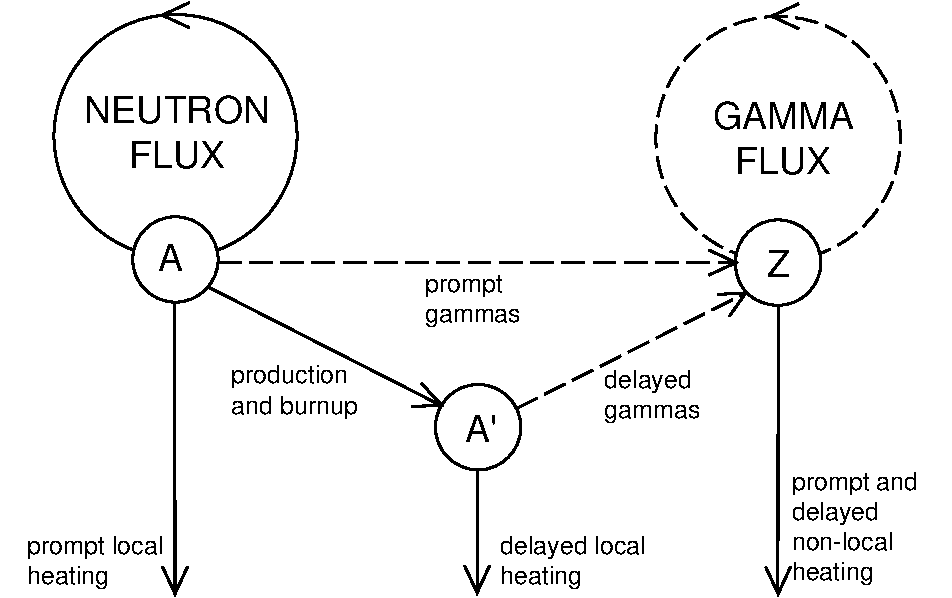
\includegraphics[height=3.4in, angle=0]{figs/heatr1}
\caption[Components of nuclear heating]{Components of nuclear
   heating.  HEATR treats the prompt
   local neutron heating only.  Gamma heating is computed
   in \hyperlink{sGAMINRhy}{GAMINR}.  Delayed local heating
   and photon production are
   not treated by NJOY, and they must be added at a later stage.}
\label{f1}
\end{figure}

Heating, therefore, is often described by
KERMA\cite{MACK}\index{KERMA} (Kinetic Energy Release in Materials)
coefficients $k_{ij}(E)$ defined such that the heating rate in a
mixture is given by

\begin{equation}
   H(E)=\sum_i\sum_j\rho_i k_{ij}(E)\phi(E)\,\,,
\label{HofE}
\end{equation}

\noindent
where $\rho_i$ is the number density of material $i$, $k_{ij}(E)$ is
the KERMA coefficient for material $i$ and reaction $j$ at incident
energy $E$, and $\phi(E)$ is the neutron or photon scalar flux at $E$.
KERMA is used just like a microscopic reaction cross section except
that its units are energy $\times$ cross section (eV-barns for HEATR).
When multiplied by a flux and number density, the result would give
heating in eV/s.

The ``direct method''\index{direct heating} for computing the KERMA
coefficient is

\begin{equation}
   k_{ij}(E)=\sum_\ell \overline{E}_{ij\ell}(E)\sigma_{ij}(E)\,\,,
\label{direct}
\end{equation}

\noindent
where the sum is carried out over all charged products of the reaction
including the recoil nucleus, and $\overline{E}_{ij\ell}$ is the total
kinetic energy carried away by the $\ell^{th}$ species of secondary
particle.  These kinds of data are now becoming available for some
materials with the advent of ENDF/B-VI and later, but earlier
ENDF/B versions did not include the detailed spectral information
needed to evaluate Eq.~\ref{direct}.

For this reason, NJOY computes KERMA factors for many materials by
the ``energy-balance method''\cite{Muir}.\index{energy-balance heating}
The energy allocated to neutrons and photons is simply subtracted
from the available energy to obtain the energy carried away by
charged particles:

\begin{equation}
   k_{ij}(E)=\Bigl(E+Q_{ij}-\overline{E}_{ijn}-\overline{E}_{ij\gamma}
      \Bigr)\,\sigma_{ij}(E)\,\,,
\label{kij}
\end{equation}
\vspace{0.5 pt}

\noindent
where $Q_{ij}$ is the mass-difference $Q$-value for material $i$ and
reaction $j$, $\overline{E}_n$ is the total energy of secondary
neutrons including multiplicity, and $\overline{E}_\gamma$ is the
energy of secondary photons including photon yields.

This method was well suited for use with ENDF/B-V\index{ENDF!ENDF/B-V},
or any other evaluation containing neutron and photon spectral
data, but not the
particle spectra required by the direct method.  The disadvantage
of this method is that the KERMA factor sometimes depends on a
difference between large numbers.  In order to obtain accurate
results, care must be taken by the evaluator to ensure
that photon and neutron yields and average energies are consistent.
In fact, the lack of consistency in ENDF/B-V often revealed itself
as negative KERMA\index{KERMA!negative KERMA} coefficients\cite{ebal}.

However, a negative KERMA coefficient is not always the defect it
seems to be.  It must be remembered that heating has both neutron and
photon components.  A negative KERMA might indicate that too much
energy has been included with the photon production in the evaluation.
This will result in excessive photon heating if most of the photons
stay in the system.  However, the negative KERMA will have just the
right magnitude to cancel this excess heating. The energy-balance
method guarantees conservation of total energy in large homogeneous
systems.

In this context, large and homogeneous means that most neutrons and
photons stay in their source regions.  It is clear that energy-balance
errors in the evaluation affect the spatial distribution of heat and
not the total system heating when the energy-balance method is
employed.

A final problem with the energy-balance method occurs for the
elemental evaluations\index{elemental heating} common in earlier
versions of ENDF/B.  Isotopic $Q$-values and cross sections
are not available in the files.  It will usually be possible to define
adequate cross sections, yields, and spectra for the element.  However,
it is clear that the available energy should be computed with an
effective Q given by

\begin{equation}
   \overline{Q}=\frac{\displaystyle\sum_i\rho_i\sigma_iQ_i}
      {\displaystyle\sum_i\rho_i\sigma_i}\,\,,
\end{equation}

\noindent
where $\rho_i$ is the atomic fraction of isotope $i$ in the element.
This number is energy dependent and can be represented only
approximately by the single constant Q allowed
in ENDF/B.  HEATR allows the user to input an auxiliary
energy-dependent Q for elements.\index{energy-dependent Q}

For elastic and discrete-level inelastic scattering, the neutron
KERMA coefficient can be evaluated directly without reference to
photon data.  For other reactions, conservation of momentum and
energy can be used to estimate the KERMA or to compute minimum and
maximum limits for the heating.  HEATR includes an option that tests
the energy-balance KERMA factors against these kinematic limits,
\index{kinematic heating tests} thereby providing a valuable test
of the neutron-photon consistency of the evaluation.  If the
energy-balance heating numbers for a particular isotope should
fail these tests, and if the isotope is important for a ``small''
system, an improved evaluation is probably required.  The
alternative of making {\it ad hoc} fixes to improve the local heat
production is dangerous because the faults in the neutron and/or photon
data revealed by the tests may lead to significant errors in neutron
transport and/or photon dose and nonlocal energy deposition.

In practice, an exception to this conclusion must be made for the
radiative capture reaction (n,$\gamma$).  The difference between the
available energy $E{+}Q$ and the total energy of the emitted photons is
such a small fraction of $E{+}Q$ that it is difficult to hold enough
precision to get reasonable recoil energies.  Moreover, the emitted
photons cause a component of recoil whose effect is not normally
included in evaluated capture spectra.  Finally, the ``element
problem'' cited above is especially troublesome for capture because
the available energy may change by several MeV between energies
dominated by resonances in different isotopes of the element, giving
rise to many negative or absurdly large heating numbers.  These
problems are more important for damage calculations (see below) where
the entire effect comes from recoil and the compensation provided by
later deposition of the photon energy is absent.

For these reasons, HEATR estimates the recoil due to radiative capture
\index{capture heating} using conservation of momentum.  The recoil
is the vector sum of the ``kick'' caused by the incident neutron
and the kicks due to the emission of all subsequent photons.  Assuming
that all photon emission is isotropic and that the directions of
photon emission are uncorrelated, the photon component of recoil
depends on the average of $E_\gamma^2$ over the entire photon spectrum

\begin{equation}
   E_R=\frac{E}{A+1}+\frac{\overline{E_\gamma^2}}{2(A+1)mc^2}\,\,,
\end{equation}
\vspace{0.5 pt}

\noindent
where $mc^2$ is the neutron mass energy.  The second term is important
below 25 -- 100 keV.  This formula gives an estimate that works for both
isotopes and elements and has no precision problems.  However, it
does not explicitly conserve energy, and isotopes with bad capture
photon data can still cause problems.

\subsection{Theory of Damage Energy}
\label{ssHEATR_damagetheory}

Damage to materials\index{radiation damage} caused by neutron
irradiation is an important design consideration in fission reactors
and is expected to be an even more important problem in fusion
power systems.  There are many radiation effects that may cause
damage, for example, direct heating, gas production ({\it e.g.},
helium embrittlement), and the production of lattice defects.

A large cluster of lattice defects can be produced by the primary
recoil nucleus of a nuclear reaction as it slows down in a lattice.
It has been shown that there is an empirical correlation between the
number of displaced atoms (DPA\index{DPA}, displacements per atom)
and various properties of metals, such as elasticity.  The number
of displaced atoms depends on the total available energy $E_a$ and
the energy required to displace an atom from its lattice position
$E_d$.  Since the available energy is used up by producing pairs,

\begin{equation}
   {\rm DPA}=\frac{E_a}{2E_d}\,\,.
\end{equation}
\vspace{0.5 pt}

\noindent
The values of $E_d$ used in practice are chosen to represent the
empirical correlations, and a wide range of values is found in the
literature\cite{Gabriel,Doran,Greenwood}.  Table~\ref{ade} gives
the default values used in NJOY2016.  The energy available to cause
displacements is what HEATR calculates.  It depends on the recoil
spectrum and the partition of recoil energy between electronic
excitations and atomic motion.  The partition function used is
given by Robinson\cite{Robinson} based on the electronic screening
theory of Lindhard\cite{Lindhard} (see Fig.~\ref{f2}).

\begin{table}[t]
\caption[Atomic Displacement Energy Data for DPA]{Typical
  Values for the Atomic Displacement Energy
  Needed to Compute DPA\cite{Greenwood}.}

\begin{center}
\begin{tabular}{cccc}
Element & $E_d$, eV & Element & $E_d$, eV \\ \hline
Be & 31 & Co & 40 \\
C  & 31 & Ni & 40 \\
Mg & 25 & Cu & 40 \\
Al & 27 & Zr & 40 \\
Si & 25 & Nb & 40 \\
Ca & 40 & Mo & 60 \\
Ti & 40 & Ag & 60 \\
V  & 40 & Ta & 90 \\
Cr & 40 & W  & 90 \\
Mn & 40 & Au & 30 \\
Fe & 40 & Pb & 25 \\ \hline
\end{tabular}
\end{center}
\label{ade}
\end{table}

\begin{figure}[t]\centering
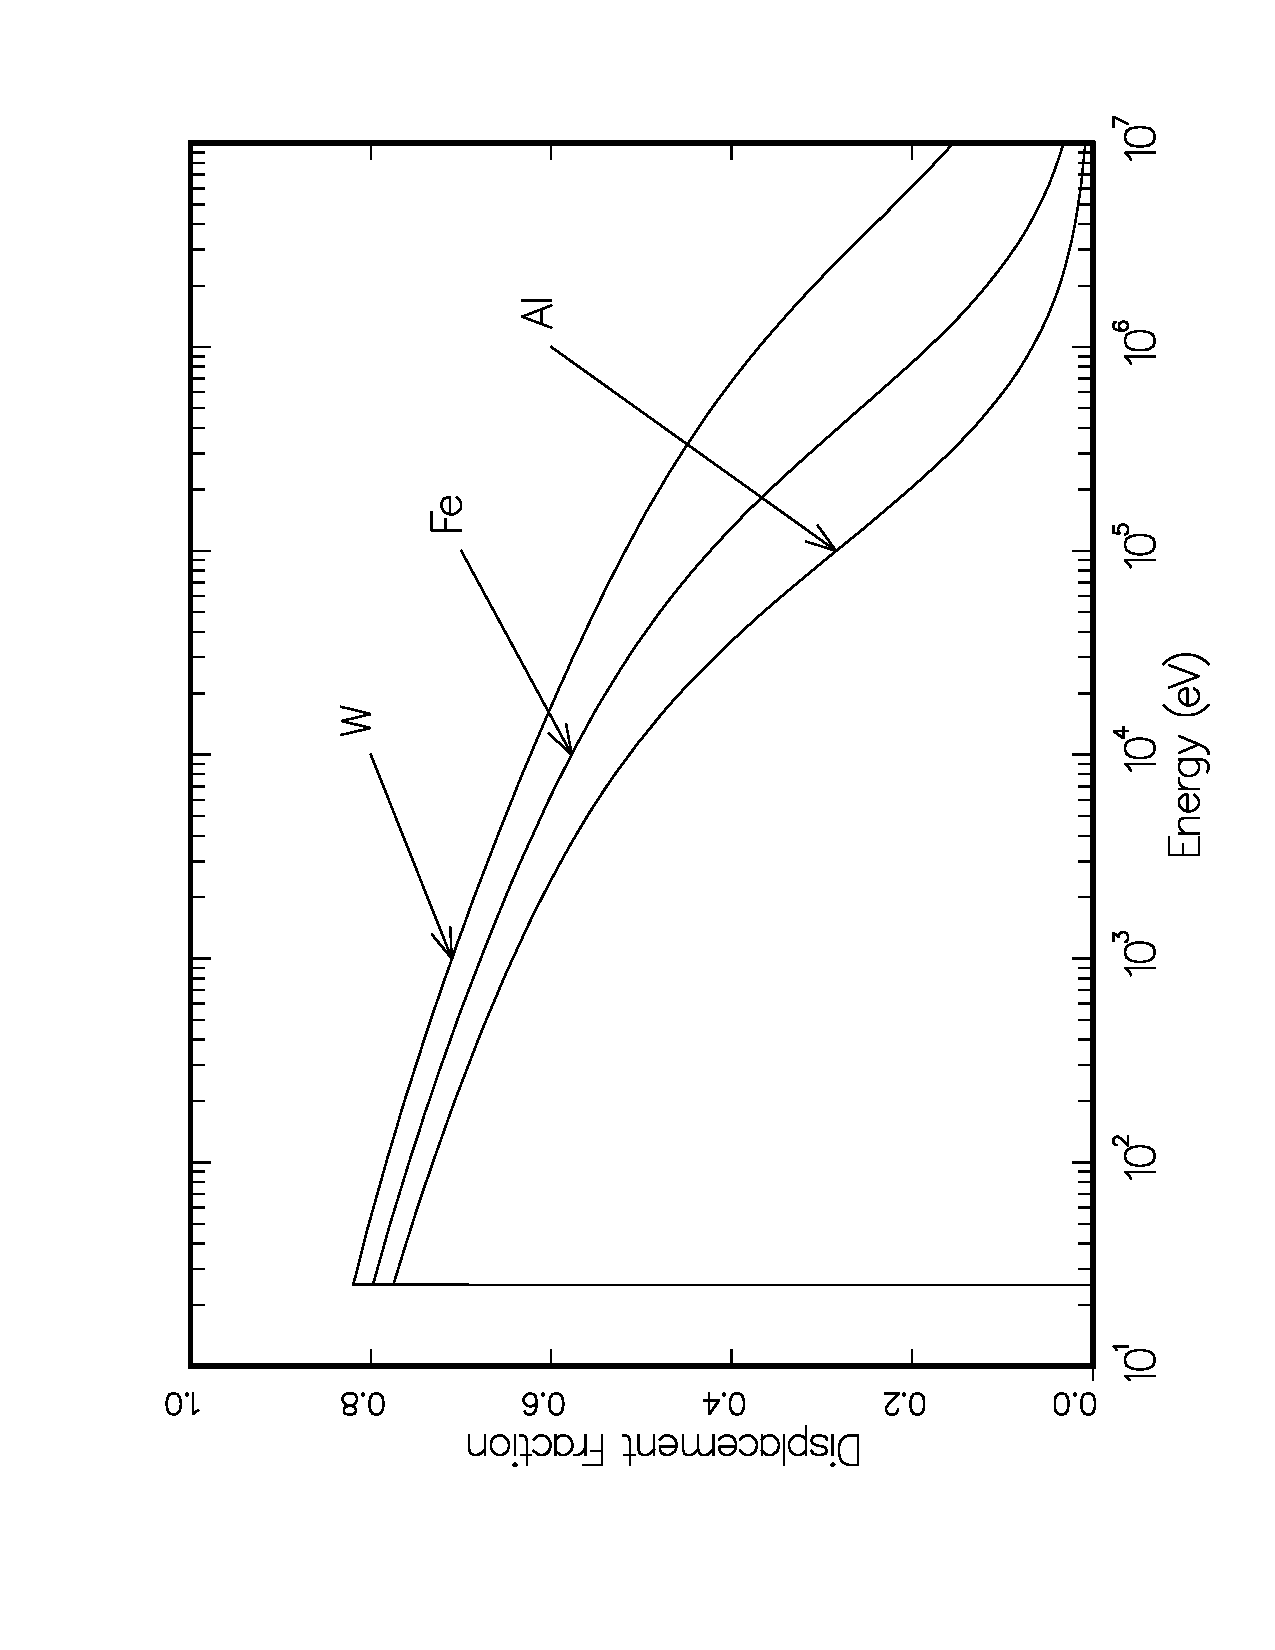
\includegraphics[height=4.0in, angle=270]{figs/heatr2ack}
\caption[Sample recoil energy and lattice displacement data]
  {Examples of the portion of the primary recoil
  energy that is available to cause lattice displacements in
  metallic lattices.  The remaining energy leads to electronic
  excitation.  The quantity plotted is $P(E)$ from
  Eq.~\ref{robinson} divided by $E$.  The 25 eV cutoff
  is also discussed in connection with Eq.~\ref{robinson}.}
\label{f2}
\end{figure}

The damage output from HEATR is the damage energy production
cross section (eV-barns).  As in Eq.~\ref{HofE}, multiplying by
the density and flux gives eV/s.  Dividing by $2E_d$ gives
displacements/s.  This result is often reduced by an efficiency
factor (say 80\%) to improve the fit to the empirical correlations.
\index{damage energy production}


\subsection{Computation of KERMA Factors By Energy Balance}
\label{ssHEATR_KERMA}

\subsubsection{The general case}
\label{sssHEATR_generalKERMA}

The older ENDF/B files do not usually give photon production data for
all partial reactions.  Summation reactions such as nonelastic
(MT=3) and inelastic (MT=4) are often used.  It is still possible
to compute partial KERMA factors for those summation reactions by
reordering Eq.~\ref{kij} as follows:

\begin{equation}
   k_{ij}=\sum_{j\in J}k_{ij}^n(E)-\sum_{\ell\in J}
    \overline{E}_{i\ell\gamma}\sigma_{i\ell}(E)\,\,,
\label{reordered}
\end{equation}
\vspace{0.5 pt}

\noindent
where $j$ runs over all neutron partials contained in $J$, and
$\ell$ runs over all photon partials in $J$.  The total KERMA is
well defined, but partial KERMAS should be used only with caution.

HEATR loops through all the neutron reactions on the ENDF/B tape.
If energy balance is to be used, it computes the neutron
contributions needed for the first term.  These are

\begin{equation}
   k_{ij}^n(E)=
    \Bigl[E+Q_{ij}-\overline{E}_{ijn}(E)\Bigr]\sigma_{ij}(E)\,\,.
\label{nkerm}
\end{equation}
\vspace{0.5 pt}

The $Q$-value is zero for elastic and inelastic scattering.  For
(n,n$'$) particle reactions represented by scattering with an
LR flag set, Q is the ENDF ``C1'' field from MF=3.  For most
other reactions, Q is the ``C2'' field from MF=3.  HEATR allows
users to override any $Q$-value with their own numbers.

The $\overline{E}_n$ value as used in Eq.~\ref{nkerm} is
defined to include multiplicity.  The multiplicity is either
implicit --- for example, 2 for (n,2n) --- or is retrieved from the
ENDF/B file (e.g. for the mt5 reaction).  The average energy per
neutron is computed differently for discrete two-body reactions
and continuum reactions.

For elastic and discrete inelastic scattering (MT=2, 51-90),

\begin{equation}
   \overline{E}_n=\frac{E}{(A+1)^2}\Bigl(1+2Rf_1+R^2\Bigr)\,\,,
\label{enb}
\end{equation}

\noindent
where $f_1$ is the center-of-mass (CM) average scattering cosine
from MF=4 and $R$ is the effective mass ratio.  For elastic
scattering, $R{=}A$, but for threshold scattering,

\begin{equation}
   R=A\sqrt{1-\frac{(A+1)S}{AE}}\,\,,
\end{equation}

\noindent
where $S$ is the negative of the C2 field from MF=3.

For continuum scattering, the average energy per neutron is
computed from the secondary neutron spectrum, $g$, in MF=5 using

\begin{equation}
   \overline{E}_n(E)=\int_0^U E'g(E,E')\,dE'\,\,,
\end{equation}

\noindent
where $U$ is defined in MF=5.  If $g$ is tabulated (LAW=1 or
LAW=5), the integral is carried out analytically for each panel
by making use of the ENDF/B interpolation laws.  For the simple
analytic representations (LAW=7, 9, or 11), the average energies
are known\cite{ENDF102}.

The neutron cross sections required by Eq.~\ref{nkerm} are
obtained from an existing PENDF\index{PENDF} file (see
\hyperlink{sRECONRhy}{RECONR}\index{RECONR},
and \hyperlink{sBROADRhy}{BROADR})\index{BROADR}.

When the neutron sum in Eq.~\ref{reordered} is complete, the
code processes the photon production files.  If the evaluation
does not include photon data, HEATR returns only the first sum.
This is equivalent to assuming that all photon energy is
deposited locally, consistent with the fact that there will
be no contribution to the photon transport source from this
material.  The same result can be forced by using the
\cword{local} parameter (see ``User Input'', Section~\ref{ssHEATR_inp}, below).

Discrete photon yields and energies are obtained from
MF=12 or 13.  Continuum photon data are obtained from MF=15,
and the average photon energy and $\overline{E_\gamma^2}$ are
computed.  For radiative capture, the photon term becomes

\begin{equation}
   E_\gamma\sigma_\gamma=\left(E+Q-\frac{E}{A+1}
    +\frac{\overline{E_\gamma^2}}{2(A+1)mc^2}\,Y_\gamma\right)
    \sigma_\gamma\,\,,
\label{cfix}
\end{equation}

\noindent
\cite{ENDF102}
where $Y_\gamma$ is the capture photon yield from MF=12.  This
corrects the capture contribution from Eq.~\ref{nkerm} by
conservation of momentum.  For other reactions,
Eq.~\ref{nkerm} is sufficient, and the product of
$\overline{E}_\gamma$, $Y_\gamma$, and $\sigma_\gamma$ is
subtracted from the neutron contribution.

\subsubsection{The special case of fission}
\label{sssHEATR_fissionKERMA}

The partial KERMA for fission is a special case due to the particular
problems with obtaining the $Q$-value for fission\index{fission Q}.
First, the fission $Q$-value given in the C1 field of MF=3 includes
delayed neutron and gamma contributions that we need to exclude,
and second, the $Q$-value for fission is energy dependent.

As a result, the KERMA for fission will be calculated differently
when compared to the other reactions which use Eq.~\ref{nkerm} as is.
Theoretically speaking, there is no difference with Eq.~\ref{nkerm}
as we will show here.

Energy dependent fission energy release and its components are given
in the MT=458 section of MF=1 on the ENDF file. This section of the
ENDF file defines the following components to the fission energy release:
\begin{itemize}
\item $Q_k$ : the kinetic energy of the fission fragments
\item $Q_{n,p}$ and $Q_{n,d}$ : the kinetic energy of the prompt and
      delayed fission neutrons
\item $Q_{\gamma,p}$ and $Q_{\gamma,d}$ : the energy of the prompt
      and delayed gamma rays
\item $Q_{\beta}$ : the energy of the delayed beta radiation
\item $Q_{\nu}$ : the energy carried away by the neutrinos
\end{itemize}

With these components, we can now define the total energy release
from fission $Q_t$, the total energy release from fission excluding
neutrinos $Q_r$ and the total prompt energy release from fission
$Q_p$ as as follows:
\begin{equation}
   Q_t(E) = Q_k(E) + Q_{n,p} + Q_{n,d} + Q_{\gamma,p} + Q_{\gamma,d}
          + Q_{\beta} + Q_{\nu}\,\,,
\end{equation}
\begin{equation}
   Q_r(E) = Q_t(E) - Q_{\nu}\,\,,
\end{equation}
\begin{equation}
   Q_p(E) = Q_r(E) - Q_{n,d} - Q_{\gamma,d} - Q_{\beta}
          = Q_k(E) + Q_{n,p} + Q_{\gamma,p}\,\,.
\end{equation}

Using these fission energy release components, we can define the
fission reaction $Q$-value (i.e. the energy released through the fission
reaction) as the prompt fission energy release minus the incident
neutron energy:
\begin{equation}
   Q(E) = Q_p(E) - E
        = Q_k(E) + Q_{n,p} + Q_{\gamma,p} - E\,\,.
\end{equation}

It should be noted that we have chosen to ignore the energy dependence
of delayed beta and gamma emission because we don't yet treat it in
subsequent codes. However, the impact of such an approximation is somewhat
limited due to the amount of energy involved. For example, for U235 the
value of $Q_k$ is roughly 169 MeV at 1e-5 eV while the sum of $Q_{n,d}$,
$Q_{\gamma,d}$ and $Q_{\beta}$ is roughly 12 MeV at 1e-5 eV.

For the calculation of the fission KERMA factor, we also need to know the
energy of the outgoing neutrons (i.e. $\overline{E}$ from Eq.~\ref{nkerm}).
Because we are considering the prompt energy release only, this is simply
equal to the prompt neutron energy release $Q_{n,p}$.

As a result, the partial fission KERMA factor $k_{f}^n$ will be given by:
\begin{equation}
   k_{f}^n(E)=
    \Bigl[E + Q(E) - \overline{E}(E)\Bigr]\sigma_{f}(E)
             =
    \Bigl[Q_k(E) + Q_{\gamma,p}(E)\Bigr]\sigma_{f}(E)\,\,.
\label{fkerm}
\end{equation}

The fission KERMA is thus equal to the fission cross section times the
sum of the kinetic energy of the fission products and the prompt gamma
energy release. This value will then be used in Eq.~\ref{reordered} to
calculate the total KERMA.

In some cases it is possible that a fissile nuclide does not have an
MT458 section. In this case, Eq.~\ref{nkerm} will be used directly as
follows:
\begin{equation}
   k_{f}^n(E)=
    \Bigl[E + Q(E) - \overline{\nu}(E)\overline{E}(E)\Bigr]\sigma_{f}(E)
\label{fkerm-nomt458}
\end{equation}
where the fission $Q$-value is approximated using the thermal point
energy dependencies defined for MT458:
\begin{equation}
   Q(E) = Q_{\text{ENDF}} - 8070000 \left(\overline{\nu}(E)-\overline{\nu}(0)\right) + 0.307 E
\end{equation}

In this equation, $Q_{\text{ENDF}}$ is the reaction $Q$-value for fission
as given in MF3.

\subsection{Kinematic Limits}
\label{ssHEATR_kinematiclimits}

As an option provided  mainly as an aid to evaluators, HEATR
will compute the kinematic maximum and minimum KERMA
\index{kinematic limits} coefficients and compare them with the
energy-balance results.  The formulas are as follows.  For
elastic scattering (MT=2), the expected recoil energy is

\begin{equation}
   \overline{E}_R=\frac{2AE}{(A+1)^2}(1-f_1)\,\,.
\end{equation}

For discrete-inelastic scattering (MT=51-90), the photon
momentum is neglected to obtain

\begin{equation}
   \overline{E}_R=\frac{2AE}{(A+1)^2}\left[\,1-
    f_1\sqrt{1-\frac{(A+1)E_\gamma}{AE}}\,\,\right]
    -\frac{E_\gamma}{A+1}\,\,,
\label{disc}
\end{equation}

\noindent
where $E_\gamma{=}-$C2 from MF=3.  For continuum inelastic
scattering (MT=91), secondary neutrons are assumed to be
isotropic in the laboratory system (LAB) giving

\begin{equation}
   \overline{E}_R=\frac{E-E_n}{A}\,\,,
\label{contin}
\end{equation}

\noindent
and

\begin{equation}
   \overline{E}_\gamma=
     \frac{(A-1)E-(A+1)\overline{E}_n}{A}\,\,,
\label{contin2}
\end{equation}
\vspace{0.5 pt}

\noindent
where $\overline{E}_\gamma$ is the average photon energy
expected for this representation.  For radiative capture (MT=102),

\begin{equation}
   \overline{E}_R=\frac{E}{A+1}+E_K
\end{equation}

\noindent
and

\begin{equation}
   \overline{E}_\gamma=Q+\frac{AE}{A+1}-E_K\,\,,
\end{equation}

\noindent
where

\begin{equation}
   E_K=\frac{1}{2M_Rc^2}\left[\frac{AE}{A+1}+Q\right]^2
     \left\{1-\frac{1}{M_Rc^2}\left[
       \frac{AE}{A+1}+Q\right]\right\}\,\,,
\end{equation}

\noindent
with

\noindent
\begin{equation}
   M_Rc^2=(939.565\times 10^6)(A+1)-Q
\end{equation}

\noindent
being the mass energy in eV.  The value of this constant is
actually computed from fundamental constants in NJOY2016.

For two-body scattering followed by particle emission
(MT=51-91, LR flag set), a minimum and maximum can be defined:

\begin{eqnarray}
   (E'_R+E_x)_{\rm min}&=&\overline{E}_R\,\,,\;\hbox{and}\\
   (E'_R+E_x)_{\rm max}&=&\overline{E}_R+Q+(E_\gamma)_{\rm max}\,\,,
\end{eqnarray}

\noindent
where $\overline{E}_R$ is the value from Eq.~\ref{disc} or
(\ref{contin}), $Q$ is the C2 field from File 3, and
$(E_\gamma)_{\rm max}$ is the negative of the C2 field from
File 3.  In these equations, $E'_R$ is the recoil energy
and $E_x$ is the energy of the charged product.  For
absorption followed by particle emission (MT=103-120),

\begin{eqnarray}
   (E_R+E_x)_{\rm min}&=&\frac{E}{A+1-x}\,\,,\\
   (E_\gamma)_{\rm max}&=&Q+\frac{A-x}{A+1-x}\,E\,\,,\;\hbox{and}\\
   (E_R+E_x)_{\rm max}&=&E+Q\,\,,
\end{eqnarray}

\noindent
where $Q$ is the C2 field from MF=3 and $x$ is the particle mass
ratio ($x{=}1$ gives a minimum for all reactions).
For (n,2n) reactions,

\begin{eqnarray}
   (E_R)_{\rm min}&=&0\,\,,\;\hbox{and}\\
   (E_R)_{\rm max}&=&\frac{E+\overline{E}_n}{A-1}\,\,,
\end{eqnarray}

\noindent
and for (n,3n) reactions,

\begin{eqnarray}
   (E_R)_{\rm min}&=&0\,\,,\;\hbox{and}\\
   (E_R)_{\rm max}&=&\frac{E+2\overline{E}_n}{A-2}\,\,.
\end{eqnarray}

\noindent
For both (n,2n) and (n,3n), if $(E_R)_{\rm max}$ is greater than
$E_R$, it is set equal to $E_R$.  In addition, these formulas
are not used for $A{<}10$; $(E_R)_{\rm max}$ is set to $E_R$.
For other neutron continuum scattering reactions (MT=22-45),

\begin{eqnarray}
   (E_R+E_x)_{\rm min}&=&0\,\,,\;\hbox{and}\\
   (E_R+E_x)_{\rm max}&=&E+Q-\overline{E}_n\,\,,
\end{eqnarray}

\noindent
where $Q$ is the C2 field from File 3.  Finally, for fission
(MT=18-21, 38), the limits are

\begin{eqnarray}
   (E_R)_{\rm min}&=&E+Q-\frac{1}{2}
    \overline{E}_n-15{\times}10^6\,\hbox{\rm eV}\,\,,\;\hbox{and}\\
   (E_R)_{\rm max}&=&E+Q-\overline{E}_n\,\,,
\end{eqnarray}

\noindent
where $Q$ is the prompt fission Q-value less neutrinos.  It
is determined by taking the total (less neutrinos) value from
File 3 and subtracting the delayed energy obtained from
MF=1/MT=458.

These values are intended to be very conservative.  Note
that $E_K$ is only significant at very low neutron energy.
In order to reduce unimportant error messages, a tolerance
band is applied to the above limits.  If all checks are
satisfied, the resulting KERMA coefficients should give good
local heating results even when 99.8\% of the photons
escape the local region.  More information on using the
kinematic checks to diagnose energy-balance problems in
evaluations will be found in ``Diagnosing Energy-Balance
Problems'', Section~\ref{ssHEATR_EB_Prob}.\index{energy balance consistency}

The upper kinematic limit can also be written out to the
output tape as MT=443 if desired.  It is similar to the KERMA
factors generated by the MACK code\cite{MACK}, and it is
sometimes preferable to the energy-balance KERMA for
calculating local heating for evaluations with severe
energy-balance problems.  The kinematic value in MT=443
is useful for plots (see the examples in this report).

\subsection{Computation of Damage Energy}
\label{ssHEATR_damagecomputation}

The formulas used for calculating damage energy are derived
\index{damage energy production}
from the same sources as the heating formulas given above,
except in this case, the effects of scattering angle do not
result in simple factors like $f_1$ because the Robinson
partition function is not linear.  Instead, it is
\index{Robinson partition function}
calculated as follows:

\begin{equation}
   P(E)=\frac{E_R}{1+F_L(3.4008\epsilon^{1/6}+0.40244\epsilon^{3/4}
     +\epsilon)}\,\,,
\label{robinson}
\end{equation}
\vspace{0.5 pt}

\noindent
if $E_R\ge 25.0$ eV, and zero otherwise.  In Eq.~\ref{robinson},
$E_R$ is the primary recoil energy,

\begin{eqnarray}
   \epsilon&=&\frac{E_R}{E_L}\,\,,\\
   E_L&=&30.724Z_RZ_L\left(Z_R^{2/3}+Z_L^{2/3}\right)^{1/2}
     (A_R+A_L)/A_L\,\,,\;\hbox{and}\\
   F_L&=&\frac{0.0793Z_R^{2/3}Z_L^{1/2}\left(A_R+A_L\right)^{3/2}}
      {\left(Z_R^{2/3}+Z_L^{2/3}\right)^{3/4}A_R^{3/2}A_L^{1/2}}\,\,,
\end{eqnarray}

\noindent
and $Z_i$ and $A_i$ refer to the charge and atomic number
of the lattice nuclei (L) and the recoil nuclei (R).  The
function behaves like $E_R$ at low recoil energies and then
levels out at higher energies.  Therefore, the damage-energy
production cross section is always less than the heat
production cross section.  See Fig.~\ref{f2} for examples.

For elastic and two-body discrete-level inelastic scattering,

\begin{equation}
   E_R(E,\mu)=\frac{AE}{(A+1)^2}\Bigl(1-2R\mu+R^2\Bigr)\,\,,
\label{tworec}
\end{equation}
\vspace{0.5 pt}

\noindent
where the ``effective mass'' is given by

\begin{equation}
   R=\sqrt{1-\frac{(A+1)(-Q)}{AE}}\,\,,
\end{equation}

\noindent
and $\mu$ is the CM scattering cosine.  The damage energy
production cross section is then obtained from

\begin{equation}
   D(E)=\sigma(E)\int_{-1}^1 f(E,\mu)\,
     P(E_R[E,\mu])\,d\mu\,\,,
\label{damint}
\end{equation}

\noindent
where $f$ is the angular distribution from the ENDF/B File 4.
This integration is performed with a 20-point Gauss-Legendre
quadrature.  Discrete-level reactions with LR flags to
indicate, for example, (n,n$'$)$\alpha$ reactions, are
treated in the same way at present.  The additional emitted
particles are ignored.

Continuum reactions like (n,n$'$) give a recoil spectrum

\begin{equation}
   E_R(E,E',\mu)=\frac{1}{A}\Bigl(E-2\sqrt{EE'}\mu+E'\Bigr)\,\,,
\end{equation}

\noindent
where $E'$ is the secondary neutron energy, $\mu$ is the
laboratory cosine, and the photon momentum has been neglected.
The damage becomes

\begin{equation}
   D(E)=\sigma(E)\int_0^\infty\,dE'\,\int_{-1}^1d\mu
     \, f(E,\mu)\,g(E,E')\,P(E_R[E,E',\mu])\,\,,
\label{f5dam}
\end{equation}

\noindent
where $g$ is the secondary energy distribution from File 5.
In the code, the angular distribution is defaulted to isotropic,
and a 4-point Gaussian quadrature is used for the angular
integration.  For analytic representations of $g$, an adaptive
integration to 5\% accuracy is used for $E'$; for tabulated
File 5 data, a trapezoidal integration is performed using the
energy grid of the file.  The same procedure is used for
(n,2n), (n,3n), etc., but it is not realistic for reactions
like (n,n$'$p) or (n,n$'\alpha$).  The neutron in these types of
reactions can get out of the nucleus quite easily; thus, much of
the energy available to secondary particles is typically carried
away by the charged particles\cite{alb}.  HEATR treats these
reactions in the same way as (n,p) or (n,$\alpha$).

The recoil for radiative capture must include the momentum of
the emitted photons below 25 -- 100 keV giving

\begin{equation}
   E_R=\frac{E}{A+1}-2\sqrt{\frac{E}{A+1}}
    \sqrt{\frac{E_\gamma^2}{2(A+1)mc^2}}\cos\phi
    +\frac{\overline{E_\gamma^2}}{2(A+1)mc^2}\,\,,
\label{radrec}
\end{equation}

\noindent
where $\phi$ is the angle between the incident neutron direction
and emitted photon direction.  If subsequent photons are emitted
in a cascade, each one will add an additional term of
$\overline{E_\gamma^2}$ and an additional angle.  A complete
averaging of Eq.~\ref{radrec} with respect to $P(E_R)$ would
be very difficult and would require angular correlations not
present in ENDF/B evaluations.  However, damage calculations are still
fairly crude, and an estimate for the damage obtained by
treating the neutron ``kick'' and all the photon kicks
independently should give a reasonable upper limit because

\begin{equation}
   \int_{-1}^1D(E_R)\,d\cos\phi\le
     D\left(\frac{E}{A+1}\right)+\sum_\gamma D\left(
      \frac{\overline{E_\gamma^2}}{2M_Rc^2}\right)\,\,.
\end{equation}

\noindent
The actual formula used in the code is

\begin{eqnarray}
   D(E)&=&D\left(\frac{E}{A+1}\right)
       +D\left(\frac{1}{2M_Rc^2}\left[\frac{AE}{A+1}
       +Q\right]^2\right) \nonumber\\
       &+&\sum_\gamma D\left(\frac{\overline{E^2_\gamma}}
        {2M_Rc^2}\right)-D\left(\frac{1}{2M_Rc^2}\left[
        \frac{AE}{A+1}+Q\right]^2\right)\,\,,
\label{D102}
\end{eqnarray}

\noindent
where the first line is computed in the neutron section, and
the second line is computed in the photon section.  This form
also provides a reasonable default when no photons are given.

Finally, for the (n,particle) reactions, the primary recoil
is given by

\begin{equation}
   E_R=\frac{1}{A+1}\Bigl(E^*-2\sqrt{aE^*E_a}\cos\phi+aE_a\Bigr)\,\,,
\label{npart}
\end{equation}
\vspace{1 pt}

\noindent
where $a$ is the mass ratio of the emitted particle to the neutron,
$E^*$ is given by

\begin{equation}
   E^*=\frac{A+1-a}{A+1}\,E\,\,,
\end{equation}
\vspace{1 pt}

\noindent
and the particle energy $E_a$ is approximated as being equal
to the smaller of the available energy

\begin{equation}
   Q+\frac{AE}{A+1}\,\,,
\end{equation}
\vspace{1 pt}

\noindent
or the Coulomb barrier energy

\begin{equation}
   \frac{1.029\times10^6\,zZ}{a^{1/3}+A^{1/3}}\,\,
      \hbox{\rm in eV}\,\,,
\end{equation}
\vspace{1 pt}

\noindent
where $z$ is the charge of the emitted particle and $Z$ is
the charge of the target.  A more reasonable distribution would
be desirable\cite{alb}, but this one has the advantage of
eliminating an integration, and most results are dominated by
the kick imparted by the incident neutron anyway.  The angular
distribution for the emitted particle is taken as isotropic
in the lab.  At high incident energies, direct interaction
processes would be expected to give rise to a forward-peaked
distribution, thereby reducing the
damage.  However, the
importance of this effect is also reduced by the dominance
of the neutron kick.

\begin{figure}[tp]\centering
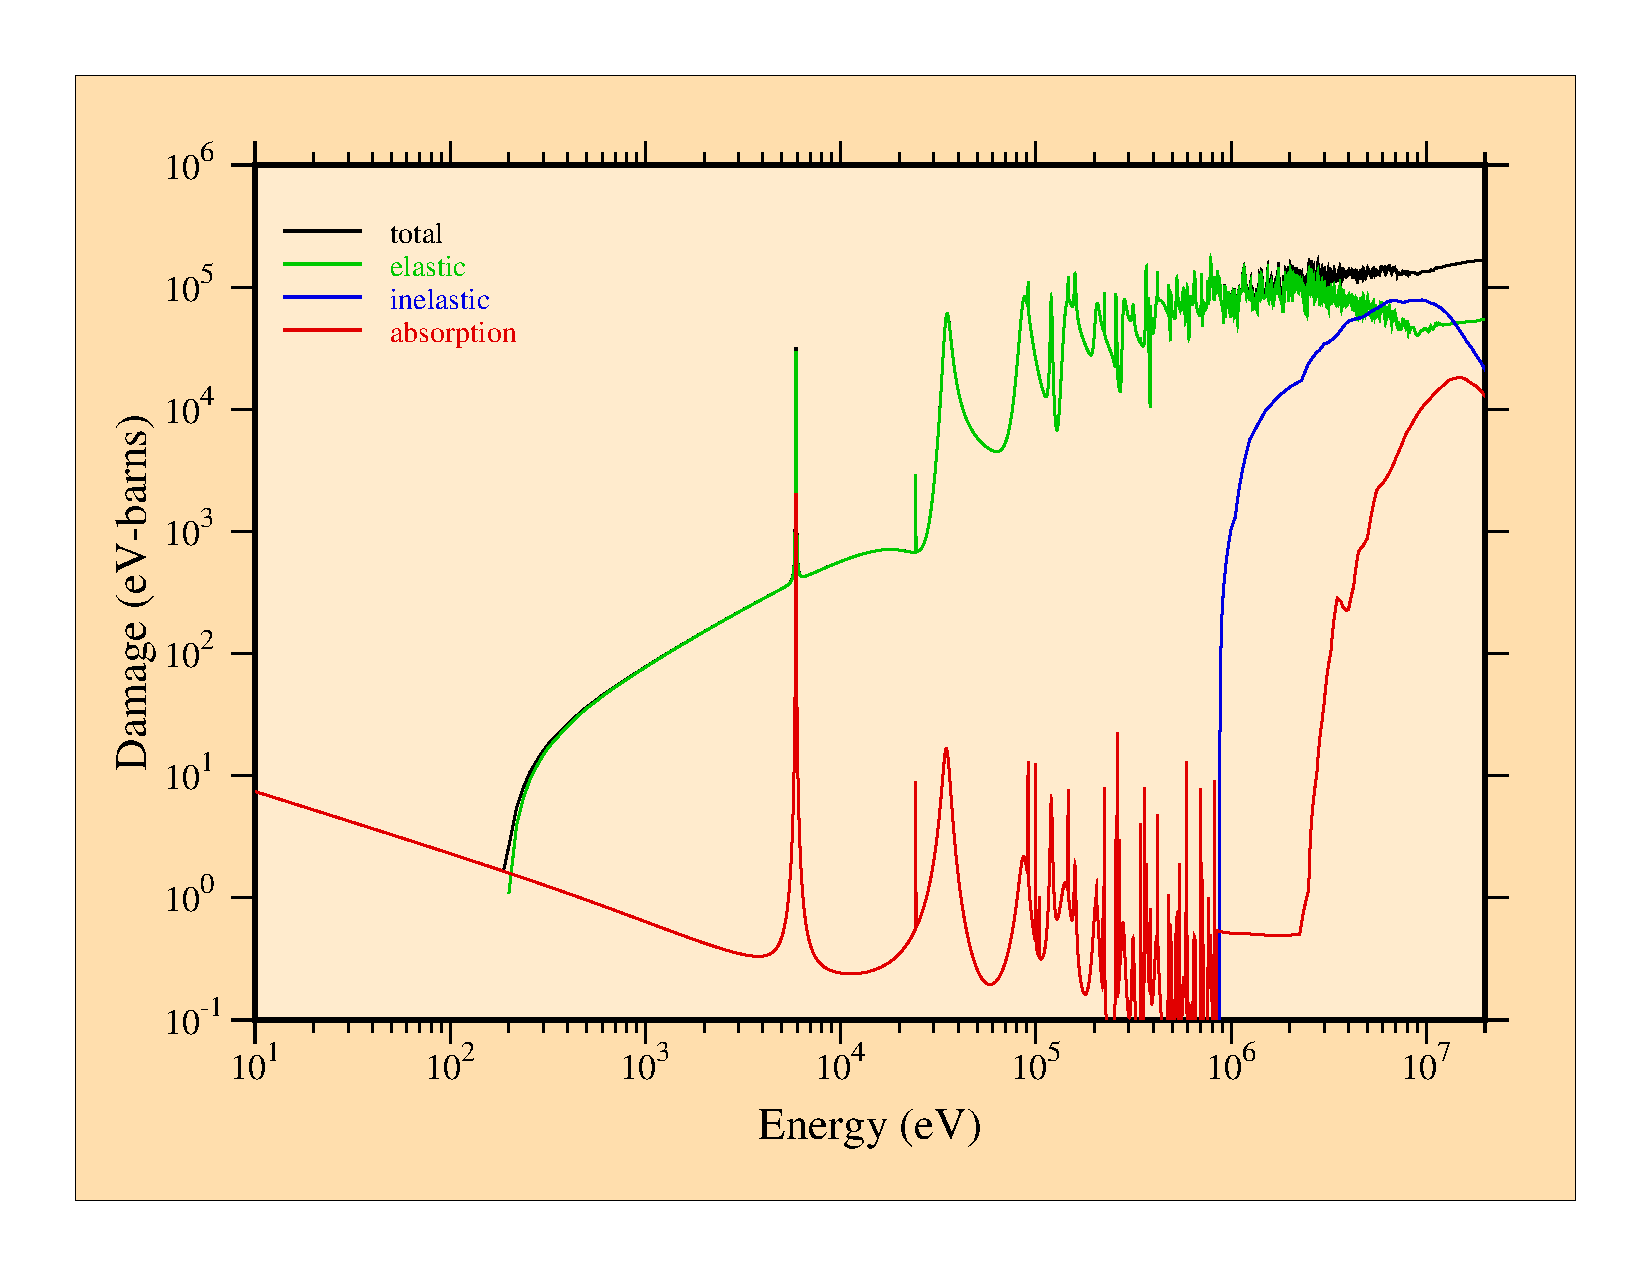
\includegraphics[keepaspectratio,height=3.2in, angle=0]{figs/heatr3ack}
\caption[Components of radiation damage energy production for $^{27}$Al]
{Components of radiation damage energy production
for $^{27}$Al from ENDF/B-VII.0.  Note that capture dominates at
very low energies, then elastic dominates, and finally inelastic
begins to contribute at very high energies.}
\label{f3}
\end{figure}

Fig.~\ref{f3} gives a typical result for a damage energy
production calculation, showing the separate contributions of
elastic, inelastic, and absorption processes.

\subsection{Heating and Damage from File 6}
\label{ssHEATR_file6}

A number of the evaluations in ENDF/B-VI and later include complete
energy-angle distributions for all of the particles produced
by a reaction, including the residual nucleus\index{recoil distributions}.
In these cases, HEATR can compute the contributions to KERMA by
calculating the average energy in the spectrum of each outgoing
charged particle or residual nucleus and using Eq.~\ref{direct}.

A fully-populated section of File 6 contains subsections for all of
the particles and photons produced by the reaction, including
the recoil nucleus.  There are a number of different schemes
used to represent the energy-angle distributions for these
outgoing particles.  The most important ones for HEATR follow:
\begin{itemize}
\begin{singlespace}
\item {\it No distribution}.  In this case, the subsection is
      inadequate for use in heating and damage calculations.
      A warning message is issued.

\item {\it Two-body angular distribution}.  These are basically
      the same as distributions in File 4.

\item {\it Recoil distribution}.  This particle is a recoil
      nucleus from a two-body reaction.  Its angular
      distribution is assumed to be the complement of the
      angular distribution for the \underbar{first} subsection
      in this section.

\item {\it CM Kalbach distribution}.  This format is often used
      by LANL evaluations, and transformation to the
      laboratory frame is required.  The looping order for
      the data is $E$, $E'$, $\mu$.

\item{\it LAB Legendre distribution}.  This format is used in
      most of the ORNL evaluations for ENDF/B-VI.  It is
      already in the laboratory frame, and the angular
      information can be simply ignored.

\item{\it LAB angle-energy distribution}.  This format is
      used for the $^{9}$Be evaluation of ENDF/B-VI by LLNL.
      The looping order is $E$, $\mu$, $E'$.
\end{singlespace}
\end{itemize}

\noindent
The normal procedure is to loop through all of these subsections.
The subsections producing neutrons are processed to be used in
a total energy check, but they contribute nothing to the heating
or to the damage. Subsections describing charged particles and
residual nuclei are processed into heating and damage contributions.
Finally, the photon subsection is processed for the photon energy
check and the total energy check, even though it does not affect
either heating or damage.  Any remaining difference between the
eV-barns available for the reaction and the eV-barns carried
away by the neutrons, photons, particles, and recoil is added
into the heating to help preserve the total energy deposition
in the spirit of the energy-balance method.

For ``two-body'' sections,  the emitted particle energy is given by

\begin{equation}
   E'=\frac{A'E}{A+1}\Bigl(1+2R\mu+R^2\Bigr) \,\,,
\label{ebar6}
\end{equation}
\vspace{1 pt}

\noindent
where

\begin{equation}
   R=\sqrt{\frac{A(A+1-A')}{A'}} \,\,,
\label{beta}
\end{equation}

\noindent
and $A'$ is the ratio of the mass of the outgoing particle to
that of the incident particle.  The heating is obtained by doing
a simple integral over $\mu$, and the damage is computed using
the integral over $\mu$ given in Eq.~\ref{damint}.  In both
cases, the integrals are performed using either a 20-point
Gauss-Legendre quadrature\index{Gauss-Legendre quadrature}
(for Legendre representations) or a trapezoidal integration
(for tabulated data).

For ``recoil'' sections, the code backs up to the particle
distribution and calculates the recoil using  the same method
described above with the sign of $\mu$ changed.

For laboratory distributions that use the $E$, $E'$, $\mu$
ordering, the angular part can be ignored, and the heating and
damage become

\begin{equation}
   K(E)=\int g(E{\rightarrow}E')E'\,dE'\,\,,
\label{KofE}
\end{equation}

\noindent
and

\begin{equation}
   D(E)=\int g(E{\rightarrow}E')P(E')\,dE'\,\,,
\label{DofE}
\end{equation}

\noindent
where $g(E{\rightarrow}E')$ is the angle-integrated energy
distribution from File 6, and $P(E')$ is the damage partition
function.  Trapezoidal integration is used for the continuum,
and the integrand is simply added into the sum for the
delta functions (if any).

Heating for subsections that use the ordering $E$, $\mu$, $E'$
is computed using the formula

\begin{equation}
   K(E)=\int \left\{ \int g(E{\rightarrow}E',\mu)
     E'\,dE'\right\} d\mu\,\,,
\label{llnl}
\end{equation}

\noindent
where an inner integral is performed using trapezoidal
integration for each value in the $\mu$ grid.  The results
are then used in a second trapezoidal integration over $\mu$.
The damage integral is performed at the same time in a
parallel manner.

The problem is somewhat more difficult for subsections
represented in the center-of-mass frame.  The definitions
for $K(E)$ and $D(E)$ are the same as those given above,
except that the quantity $g(E{\rightarrow}E')$ has to be
generated in the lab system.  The methods used to do the
transformation are basically the same in HEATR and
\hyperlink{sGROUPRhy}{GROUPR}\index{GROUPR}.  The
first step is to set up an adaptive
integration over $E'$.  The first value needed to prime the
stack is obtained by calling \cword{h6cm} with $E'{=}0$.  It
returns the corresponding value of $g$ in the lab system and
a value for \cword{epnext}.  The second value for the stack is
computed for $E$=\cword{epnext}.  The routine then subdivides
this interval until 2\% convergence is achieved, accumulating
the contributions to the heating and damage integrals as it
goes.  It then moves up to a new panel.  This process
continues until the entire range of $E'$ has been covered.

The key to this process is \cword{h6cm}\index{h6cm@{\ty h6cm}}.
As described in more detail in the
\hyperlink{sGROUPRhy}{GROUPR}\index{GROUPR} chapter
of this manual, it performs integrals of the form

\begin{equation}
   g_L(E{\rightarrow}E'_L)=\int_{\mu_{\rm min}}^{+1}
      g_C(E{\rightarrow}E'_C,\mu_C)\,J\,d\mu_L\,\,,
\label{transCM}
\end{equation}

\noindent
where $L$ and $C$ denote the laboratory and center-of-mass
systems, respectively, and $J$ is the Jacobian for the
transformation.  The contours in the $E'_C$,$\mu_C$ frame that
are used for these integrals have constant $E'_L$.  The
limiting cosine, $\mu_{\rm min}$, depends on kinematic factors
and the maximum possible value for $E'_C$ in the File 6
tabulation.

The ENDF/B-VII\index{ENDF!ENDF/B-VII} library contains a few
abbreviated versions of File 6\index{File 6} that contain an
energy-angle distribution for neutron emission, but no
recoil or photon data.  In order to get semi-reasonable
results for both heating and damage for such cases, HEATR
applies a ``one-particle recoil approximation,''
where the first particle emitted is assumed to induce all
the recoil.  There are also some cases where capture photons
are described in MF=6/MT=102 with no corresponding recoil data.
Here, the recoil can be added using the same logic described
above for capture represented using File 15.  The difference
between the eV-barns available for the reaction and the energy
accounted for by the emitted neutrons, photons, particles, and
the approximated recoil is added into the heating in order to
preserve the total heating in the spirit of the energy-balance
method.


\subsection{User Input}
\label{ssHEATR_inp}

The input instructions that follow were reproduced from the
comment cards in the current version of HEATR.
\index{HEATR!HEATR input}
\index{input!HEATR}

\small
\begin{ccode}

   !---input specifications (free format)------------------------
   !
   ! card 1
   !    nendf    unit for endf tape
   !    nin      unit for input pendf tape
   !    nout     unit for output pendf tape
   !    nplot    unit for graphical check output
   ! card 2
   !    matd     material to be processed
   !    npk      number of partial kermas desired (default=0)
   !    nqa      number of user q values (default=0)
   !    ntemp    number of temperatures to process
   !             (default=0, meaning all on pendf)
   !    local    0/1=gamma rays transported/deposited locally
   !             (default=0)
   !    iprint   print (0 min, 1 max, 2 check) (default=0)
   !    ed       displacement energy for damage
   !             (default from built-in table)
   ! card 3      for npk gt 0 only
   !    mtk      mt numbers for partial kermas desired
   !             total (mt301) will be provided automatically.
   !             partial kerma for reaction mt is mt+300
   !             and may not be properly defined unless
   !             a gamma file for mt is on endf tape.
   !             special values allowed--
   !               303   non-elastic (all but mt2)
   !               304   inelastic (mt51 thru 91)
   !               318   fission (mt18 or mt19, 20, 21, 38)
   !               401   disappearance (mt102 thru 120)
   !               442   total ev-barns
   !               443   total kinematic kerma (high limit)
   !             damage energy production values--
   !               444   total
   !               445   elastic (mt2)
   !               446   inelastic (mt51 thru 91)
   !               447   disappearance (mt102 thru 120)
   !          cards 4 and 5 for nqa gt 0 only
   ! card 4
   !    mta      mt numbers for users q values
   ! card 5
   !    qa       user specified q values (ev)
   !               (if qa.ge.99.e6, read in variable qbar
   !                  for this reaction)
   ! card 5a     variable qbar (for reactions with qa flag only)
   !    qbar      tab1 record giving qbar versus e (1000 words max)
   !
   !----------------------------------------------------------------

\end{ccode}
\normalsize

Card 1 specifies the input and output units for HEATR.  They
are all ENDF-type files.  The input PENDF file has normally
been through \hyperlink{sRECONRhy}{RECONR} and
\hyperlink{sBROADRhy}{BROADR}, but it is possible to run HEATR
directly on an ENDF file in order to do kinematic checks.  In
this case, the results in the resonance range should be
ignored. Defining \cword{nplot} will produce a file of input
for the \hyperlink{sVIEWRhy}{VIEWR}\index{VIEWR} module
containing detailed energy-balance
test results.  This option should only be used together with
\cword{iprint}=2.

On Card 2, the default value for \cword{npk} is zero, which
instructs the code to process the energy-balance total KERMA
(MT=301) only.  Most often, the user will also want to include MT=443
and MT=444 (\cword{npk}=2).  The kinematic KERMA computed
when MT=443 is requested is very useful for judging the
energy-balance consistency\index{energy balance consistency}
of an evaluation (see the subsection on ``Diagnosing
Energy-Balance Problems'', Section~\ref{ssHEATR_EB_Prob},
below).  It can also be used instead
of the energy-balance value in MT=301 when local heating effects
are important and the evaluation scores poorly in an energy-balance
check.  Damage energy production cross sections (MT=444) should be
computed for important structural materials; this expensive
calculation can be omitted for other materials.

When kinematic checks are desired, a number of additional
\cword{npk} values can be included.  They can be determined by
checking the evaluation to see what partial KERMA factors are
well defined.  For old-style evaluations that do not use File 6,
look for the MT values used in Files 12 and 13.  Many
evaluations use only MT=3 and MT=102 (or 3, 18, and 102 for
fissionable materials); in these cases, the only \cword{mtk}
values that make sense are 302, 303, and 402 (or 302, 303, 318,
and 402 for fissionable materials).  Caution: in many evaluations,
MT=102 is used at low energies and taken to zero at some
breakpoint.  MT=3 is used at higher energies.  In these
evaluations, the partial KERMA MT=402 does not make sense above
the breakpoint, and MT=3 does not make sense below it.

More complicated photon-production evaluations may include MT=4
and/or discrete-photon data in MT=51-90.  In these cases, the
user can request \cword{mtk}=304.  The same kind of energy-range
restriction discussed for MT=102 can occur for the inelastic
contributions.  Other evaluations give additional partial
reactions that can be used to check the photon production and
energy-balance consistency of an evaluation in detail.  HEATR
can handle 6 additional reactions at a time.  Multiple runs
may be necessary in complex cases.

Note that several special \cword{mtk} values are provided for
the components of the damage-energy production cross section.
They were used to prepare Fig.~\ref{f3}, and may be of interest
to specialists, but they are not needed for most libraries.

In a few cases in the past, it has been necessary to change
the $Q$-values that are normally retrieved from the ENDF tape.
In addition, it is sometimes necessary to replace the single
$Q$-value supplied in MF=3 with an energy-dependent Q function
for an element.  One example of the former occurred for $^{16}$O
for ENDF/B-V.  The first inelastic level (MT=51) decays by
pair production rather than the more normal mode of photon
emission.  In order to get the correct heating, it was necessary
to change the $Q$-value by giving Card 4 and Card 5 as follows:

\small
\begin{ccode}

   51
   -5.0294e6

\end{ccode}
\normalsize

\noindent
That is, the $Q$-value is increased by twice the electron energy
of 0.511 MeV.  Another example is the sequential (n,2n)
reaction for $^{9}$Be in ENDF/B-V.  It is necessary to include
4 changes to the $Q$-values:

\small
\begin{ccode}

   46 47 48 49/
   -1.6651e6 -1.6651e6 -1.6651e6 -1.6651e6/

\end{ccode}
\normalsize

\noindent
The next example illustrates using energy-dependent $Q$-values
\index{energy-dependent Q} for elemental titanium.  Set
\cword{nqa} equal to 3 and give the following values on
Cards 4, 5, and 5a:

\small
\begin{ccode}

   16 103 107/
   99e6 99e6 99e6/
   0. 0. 0 0 1 8
   8 2
   8.0e6 -8.14e6 9.0e6 -8.14e6 1.1e7 -8.38e6
   1.2e7 -8.74e6 1.3e7 -1.03e7 1.4e7 -1.091e7
   1.5e7 -1.11e7 2.0e7 -1.125e7/
   0. 0. 0 0 1 9
   9 2
   1.0e-5 1.82e5 4.0e6 1.82e5 5.0e6 -1.19e6
   6.0e6 -2.01e6 7.0e6 -2.20e6 8.0e6 -2.27e6
   1.4e7 -2.35e6 1.7e6 -2.43e6 2.0e7 -2.37e6/
   0. 0. 0 0 1 9
   9 2
   1.0e-5 2.182e6 6.0e6 2.182e6 7.0e6 2.10e6
   8.0e6 -3.11e5 9.0e6 -9.90e5 1.0e7 -1.20e6
   1.1e7 -1.27e6 1.4e6 -1.32e6 2.0e7 -1.48e6/

\end{ccode}
\normalsize

The next parameter on Card 2 is \cword{ntemp}.  For normal
runs, use zero, and all the temperatures on the input PENDF
tape will be processed.  For kinematic check runs, use
\cword{ntemp}=1.  The \cword{local} parameter suppresses
the processing of the photon-production files, if any.
The photon energy appears in the KERMA factors as if the
photons had very short range.  A useful way to use the
\cword{iprint} parameter is to set it to zero for normal
runs, which produce heating and damage values at all
temperatures, and to use \cword{iprint}=2 for the
energy-balance check run, which is performed for the first
temperature on \cword{nin} only.

Card 3 gives the partial KERMA and damage selection MT
numbers.  Note that the user does not include MT=301 in this
list.  It is always inserted as the first value automatically.
Giving MT=301 in this list will cause an informative message
to be issued.

Cards 4, 5, and 5a give the user's changes to the ENDF Q
values.  The way in which to use these cards was described
in connection with \cword{nqa} on Card 2.

\subsection{Reading HEATR Output}
\label{ssHEATR_output}

When full output and/or kinematic checks have been requested,
\index{HEATR!HEATR output}
HEATR loops through the reactions found in Files 3, 12, and 13.
For each reaction, it prints out information about the energies,
yields, cross sections, and contributions to heating.
The energy grid used is a subset of the PENDF grid.
At present, decade steps are used below 1 eV, factor-of-two
steps are used from 1 eV to 100 keV, quarter-lethargy steps
are used above 100 keV, and approximately 1 MeV steps are used
above 2 MeV.  An example of this printout for elastic scattering
in ENDF/B-VII.0 $^{27}$Al is shown below:

\small
\begin{ccode}

 neutron heating for mt  2   q0 =  0.0000E+00     q =  0.0000E+00
            e          ebar   ...       xsec       heating        damage
   1.0000E-05    9.3052E-06   ... 1.5694E+01    1.0903E-05    0.0000E+00
   1.0000E-04    9.3052E-05   ... 5.1179E+00    3.5557E-05    0.0000E+00
   1.0000E-03    9.3052E-04   ... 2.0644E+00    1.4342E-04    0.0000E+00
   1.0000E-02    9.3052E-03   ... 1.4925E+00    1.0369E-03    0.0000E+00
   1.0000E-01    9.3052E-02   ... 1.4318E+00    9.9474E-03    0.0000E+00
     ...
   1.0000E+03    9.3052E+02   ... 1.3662E+00    9.4914E+01    7.7171E+01
   2.0000E+03    1.8610E+03   ... 1.3196E+00    1.8337E+02    1.5115E+02
   5.0000E+03    4.6526E+03   ... 1.2130E+00    4.2136E+02    3.3998E+02
   1.0000E+04    9.3052E+03   ... 1.0367E+00    7.2028E+02    5.6725E+02
   2.0000E+04    1.8610E+04   ... 6.6204E-01    9.1991E+02    7.0347E+02
   5.0000E+04    4.6526E+04   ... 2.3220E+00    8.0660E+03    5.8732E+03
   1.0000E+05    9.3052E+04   ... 5.2976E+00    3.6805E+04    2.5521E+04
     ...
   1.0000E+07    9.7233E+06   ... 7.4942E-01    2.0738E+05    4.5689E+04
   1.1000E+07    1.0699E+07   ... 7.4953E-01    2.2576E+05    4.7347E+04
   1.2000E+07    1.1682E+07   ... 7.6363E-01    2.4286E+05    4.9202E+04
   1.3000E+07    1.2673E+07   ... 7.6329E-01    2.4980E+05    4.9559E+04
   1.4000E+07    1.3670E+07   ... 7.7918E-01    2.5737E+05    5.0566E+04
   1.5000E+07    1.4671E+07   ... 7.9297E-01    2.6088E+05    5.1189E+04
   1.6000E+07    1.5676E+07   ... 8.1414E-01    2.6347E+05    5.1973E+04
   1.7000E+07    1.6681E+07   ... 8.3429E-01    2.6577E+05    5.2680E+04
   1.8000E+07    1.7689E+07   ... 8.4524E-01    2.6246E+05    5.2747E+04
   1.9000E+07    1.8695E+07   ... 8.7093E-01    2.6568E+05    5.3787E+04
   2.0000E+07    1.9703E+07   ... 8.9326E-01    2.6547E+05    5.4573E+04
     ...
   1.4000E+08    1.3985E+08   ... 2.9730E-01    4.3523E+04    1.4994E+04
   1.4600E+08    1.4585E+08   ... 2.7580E-01    4.1851E+04    1.3890E+04
   1.5000E+08    1.4984E+08   ... 2.6510E-01    4.1161E+04    1.3339E+04

\end{ccode}
\normalsize

\noindent
Note the identification and Q information printed on the first
line; \cword{q} is the ENDF $Q$-value from File 3, and \cword{q0} is
the corresponding mass-difference $Q$-value needed for Eq.~\ref{kij}.
The \cword{ebar}, \cword{yield} (which was replaced by ``...''
to make this listing fit better), and \cword{xsec} columns contain
$\overline{E}_n$, $Y$, and $\sigma$, respectively.   The
\cword{heating} column is just $(E{+}Q{-}Y\overline{E}_n)\sigma$.
The results are similar for discrete inelastic levels represented
using File 4.  The heating due to the associated photons will be
subtracted later while MF=12 or MF=13 is being processed.  However,
if an LR flag is set, the residual nucleus from the (n,n$'$)
reaction breaks up by emitting additional particles.  This extra
breakup energy changes the \cword{q0} value.  An example of such
a section for $^{27}$Al(n,n$_{25}$)p from ENDF/B-V follows:

\small
\begin{ccode}

 neutron heating for mt 75   q0 = -8.2710e+06     q = -1.0750e+07
              e          ebar         yield          xsec       heating
     1.2000e+07    7.8653e+05    1.0000e+00    8.2242e-02    2.4199e+05
     1.3000e+07    1.7116e+06    1.0000e+00    8.0121e-02    2.4176e+05
     1.4000e+07    2.6427e+06    1.0000e+00    5.9282e-02    1.8296e+05
     1.5000e+07    3.5864e+06    1.0000e+00    4.1834e-02    1.3147e+05
     1.6000e+07    4.5096e+06    1.0000e+00    2.8880e-02    9.2977e+04
     1.7000e+07    5.4335e+06    1.0000e+00    1.9867e-02    6.5472e+04
     1.8000e+07    6.3848e+06    1.0000e+00    1.3677e-02    4.5739e+04
     1.9000e+07    7.2944e+06    1.0000e+00    9.4771e-03    3.2550e+04
     2.0000e+07    8.2479e+06    1.0000e+00    6.6142e-03    2.3025e+04

\end{ccode}
\normalsize

\noindent
Starting with ENDF/B-VI, discrete-inelastic sections may also be
given in File 6.  Such sections contain their own photon
production data, and the \cword{heating} column will represent
the entire recoil energy as in Eq.~\ref{disc}.
(See below for detailed discussion of ENDF/B-VI output.)

For continuum reactions that use MF=4 and MF=5, such as (n,n$'$) or
(n,2n), the neutron part of the display looks like this:

\small
\begin{ccode}

 neutron heating for mt 16   q0 = -1.3057e+07     q = -1.3057e+07
              e          ebar         yield          xsec       heating
     1.4000e+07    1.9960e+05    2.0000e+00    2.4000e-02    1.3051e+04
     1.5000e+07    6.6850e+05    2.0000e+00    1.2320e-01    7.4659e+04
     1.6000e+07    1.0855e+06    2.0000e+00    2.0710e-01    1.5987e+05
     1.7000e+07    1.4308e+06    2.0000e+00    2.6510e-01    2.8667e+05
     1.8000e+07    1.6379e+06    2.0000e+00    3.0300e-01    5.0518e+05
     1.9000e+07    1.7659e+06    2.0000e+00    3.3000e-01    7.9567e+05
     2.0000e+07    1.8755e+06    2.0000e+00    3.5000e-01    1.1172e+06

\end{ccode}
\normalsize

\noindent
Once again, the photon effects will be subtracted later.

Absorption reactions such as (n,$\gamma$) or (n,p), lead to
similar displays, but the particle \cword{ebar} columns will
always be set to zero (no emitted neutrons).  An example
follows:

\small
\begin{ccode}

 neutron heating for mt103   q0 = -1.8278e+06     q = -1.8278e+06
              e          ebar         yield          xsec       heating
     2.5000E+06    0.0000E+00    1.0000E+00    3.2800E-05    2.2048E+01
     3.0000E+06    0.0000E+00    1.0000E+00    1.3300E-03    1.5590E+03
     3.5000E+06    0.0000E+00    1.0000E+00    1.0100E-02    1.6889E+04
     4.0000E+06    0.0000E+00    1.0000E+00    6.9667E-03    1.5133E+04
     4.5000E+06    0.0000E+00    1.0000E+00    1.7000E-02    4.5427E+04
     5.0000E+06    0.0000E+00    1.0000E+00    2.3300E-02    7.3912E+04
        ...
     1.7000E+07    0.0000E+00    1.0000E+00    5.5200E-02    8.3751E+05
     1.8000E+07    0.0000E+00    1.0000E+00    4.7800E-02    7.7303E+05
     1.9000E+07    0.0000E+00    1.0000E+00    4.0200E-02    6.9032E+05
     2.0000E+07    0.0000E+00    1.0000E+00    3.2200E-02    5.8514E+05

\end{ccode}
\normalsize

If File 6 is present (which happens for evaluations in ENDF-6
format only, such as the evaluations in ENDFB-VII), each reaction
will be divided into subsections, one for each emitted particle.
The neutron subsections are displayed as part of the energy-balance
checks, but they do not contribute to KERMA or damage.  The
subsection for each charged particle or residual nucleus will
give the incident energy, average energy for the emitted particle,
cross section, heating contribution, and (optionally) damage
contribution as follows:

\small
\begin{ccode}

 file six heating for mt 28, particle =     1     q =  -8.2721E+06
              e          ebar         yield          xsec       heating
     9.0000E+06    1.2303E+05    1.0000E+00    1.0385E-03    0.0000E+00
     1.0000E+07    4.6746E+05    1.0000E+00    1.3526E-02    0.0000E+00
     ...
     1.8000E+07    3.1862E+06    1.0000E+00    3.7721E-01    0.0000E+00
     1.9000E+07    3.4535E+06    1.0000E+00    3.7577E-01    0.0000E+00
     2.0000E+07    3.7207E+06    1.0000E+00    3.7434E-01    0.0000E+00

 file six heating for mt 28, particle =  1001     q =  -8.2721E+06
              e          ebar         yield          xsec       heating
     9.0000E+06    4.5909E+05    1.0000E+00    1.0385E-03    4.7677E+02
     1.0000E+07    8.9616E+05    1.0000E+00    1.3526E-02    1.2121E+04
     ...
     1.8000E+07    3.5193E+06    1.0000E+00    3.7721E-01    1.3275E+06
     1.9000E+07    3.8257E+06    1.0000E+00    3.7577E-01    1.4376E+06
     2.0000E+07    4.1321E+06    1.0000E+00    3.7434E-01    1.5468E+06

 file six heating for mt 28, particle = 12026     q =  -8.2721E+06
              e          ebar         yield          xsec       heating
     9.0000E+06    3.2104E+05    1.0000E+00    1.0385E-03    3.3340E+02
     1.0000E+07    3.8540E+05    1.0000E+00    1.3526E-02    5.2128E+03
     ...
     1.8000E+07    8.0820E+05    1.0000E+00    3.7721E-01    3.0486E+05
     1.9000E+07    8.6147E+05    1.0000E+00    3.7577E-01    3.2372E+05
     2.0000E+07    9.1475E+05    1.0000E+00    3.7434E-01    3.4243E+05

 file six heating for mt 28, particle =     0     q =  -8.2721E+06
              e          ebar         yield          xsec       heating
     9.0000E+06    1.8347E+05    2.8104E-06    1.0385E-03    0.0000E+00
                                                     ebal   -1.8204E+02
     1.0000E+07    4.4913E+05    3.0441E-05    1.3526E-02    0.0000E+00
                                                     ebal   -2.8626E+02
     ...
     1.8000E+07    1.8309E+06    1.2028E+00    3.7721E-01    0.0000E+00
                                                     ebal    4.5397E+03
     1.9000E+07    1.8856E+06    1.3695E+00    3.7577E-01    0.0000E+00
                                                     ebal    1.8336E+03
     2.0000E+07    1.9403E+06    1.5363E+00    3.7434E-01    0.0000E+00
                                                     ebal   -7.6798E+03

\end{ccode}
\normalsize

\noindent
Note that the last subsection in this example was for emitted
photons.  Photons do not contribute to the KERMA or damage, but
this information is used to check the total energy conservation
for this reaction.  The \cword{ebal} lines show the difference
between the available energy and the sum over all the outgoing
particles. The values should be a small percentage of the total
heating.  If the \cword{ebal} values are too large, there may be
an error in the evaluation, or it may be necessary to refine the
energy grids in the distributions.  In addition, this photon
production information is needed later for the photon energy check.

After all the sections corresponding to MT numbers in File 3
have been processed (using the File 4, File 4/5, or File 6
method as appropriate), the photon production sections in
Files 12 and 13 are processed, if present.  File 12 data are
usually present for radiative capture (MT=102), at least at low
energies.  Simple files normally give a tabulated photon spectrum.
The display gives the average energy for this spectrum in the
\cword{ebar} column and the negative contribution to the
heating computed with Eq.~\ref{cfix} in the \cword{heating}
column.  The \cword{edam} column contains the
$\overline{E^2_\gamma}$ term needed to compute the photon
contribution to the damage, which is given in the \cword{damage}
column.  See Eq.~\ref{D102}.  The display also has an extra
line for each incident energy containing the percent error
``\cword{--- pc}'' between the total photon energy as computed
from File 12 and the value $E{+}Q{-}E/(A{+1})$ computed
from File 3.  As discussed above, HEATR does not guarantee energy
balance in large systems if this error occurs.  The following
example shows some large errors due to mistakes in the ENDF/B-V
evaluation for $^{55}$Mn.  Two columns labeled \cword{edam} and
\cword{xsec} have been removed to show the \cword{heating} and
\cword{damage} columns.  The text has also been shifted to the
left of its normal position to fit better on the printed page.

\small
\begin{ccode}

 photon energy (from yields) mf12, mt102
          e    ebar/err        egam ...      yield     heating      damage
 1  continuum gammas
 1.0000e-05  4.5088e+06  2.4237e+02 ... 2.4791e+00 -4.8477e+09  5.4975e+04
 1.0000e-05    53.7 pc
 1.0703e-04  4.5088e+06  2.4237e+02 ... 2.4791e+00 -1.4819e+09  1.6806e+04
 1.0703e-04    53.7 pc
 1.2520e-03  4.5088e+06  2.4237e+02 ... 2.4791e+00 -4.3347e+08  4.9159e+03
 1.2520e-03    53.7 pc
   ...
 1.3571e+04  4.4522e+06  2.3887e+02 ... 2.4836e+00 -7.3869e+03 -1.2406e-01
 1.3571e+04    51.8 pc
 2.7142e+04  4.3957e+06  2.3536e+02 ... 2.4881e+00 -3.7037e+05 -1.6487e+01
 2.7142e+04    49.9 pc
 5.4287e+04  4.2826e+06  2.2834e+02 ... 2.4972e+00 -2.5604e+04 -2.5340e+00
 5.4287e+04    46.0 pc
 1.0858e+05  4.0563e+06  2.1430e+02 ... 2.5154e+00 -1.3327e+04 -2.7289e+00
 1.0858e+05    38.3 pc

\end{ccode}
\normalsize

Many MF=12, MT=102 sections give multiplicities for the production
of discrete photons.  In these cases, HEATR prints out data for
all of the parts, and it provides a sum at the end.  The
balance error is printed with the sum.  The following example shows
a case with discrete photons.  The last two columns have been
removed (\cword{heating}, \cword{damage}), and the text has been
compacted and shifted to the left to fit on the printed page.

\small
\begin{ccode}

  photon energy (from yields) mf12, mt102
           e    ebar/err        egam        edam        xsec       yield
  1   7.7260E+06 ev gamma
  1.0000e-05  7.7260e+06  1.1448e+03  8.9780e+02  1.1677e+01  3.0000e-01
  1.1406e-04  7.7260e+06  1.1448e+03  8.9780e+02  3.4574e+00  3.0000e-01
  1.1406e-03  7.7260e+06  1.1448e+03  8.9780e+02  1.0934e+00  3.0000e-01
    ...
  2.0000e+07  2.7005e+07  1.1448e+03  8.9780e+02  1.0000e-03  3.0000e-01
  2   7.6950e+06 ev gamma
  1.0000e-05  7.6950e+06  1.1356e+03  8.9091e+02  1.1677e+01  5.0000e-02
  1.1406e-04  7.6950e+06  1.1356e+03  8.9091e+02  3.4574e+00  5.0000e-02
    ...
  2.0000e+07  2.6974e+07  1.1356e+03  8.9091e+02  1.0000e-03  5.0000e-02
  3   6.8630e+06 ev gamma
  1.0000e-05  6.8630e+06  9.0330e+02  7.1515e+02  1.1677e+01  1.2000e-03
  1.1406e-04  6.8630e+06  9.0330e+02  7.1515e+02  3.4574e+00  1.2000e-03
  1.1406e-03  6.8630e+06  9.0330e+02  7.1515e+02  1.0934e+00  1.2000e-03
    ...
 89   3.1000e+04 eV gamma
  1.0000e-05  3.1000e+04  1.8430e-02  0.0000e+00  1.1677e+01  2.8884e-01
  1.0000e-05     0.0 pc
  1.1406e-04  3.1000e+04  1.8430e-02  0.0000e+00  3.4574e+00  2.8884e-01
  1.1406e-04     0.0 pc
  1.1406e-03  3.1000e+04  1.8430e-02  0.0000e+00  1.0934e+00  2.8884e-01
  1.1406e-03     0.0 pc
  1.1912e-02  3.1000e+04  1.8430e-02  0.0000e+00  3.3832e-01  2.8884e-01
  1.1912e-02     0.0 pc
    ...
  2.0000e+07  3.1000e+04  1.8430e-02  0.0000e+00  1.0000e-03  2.8884e-01
  2.0000e+07     0.0 pc

\end{ccode}
\normalsize

\noindent
In this case ($^{27}$Al), the capture energy production checks out
perfectly for the sum of all 89 discrete photons.

Other sections using either File 12 or File 13 generate displays
similar to the following:

\small
\begin{ccode}

 photon energy (from xsecs) mf13, mt  3
              e          ebar          xsec        energy       heating
     1  continuum gammas
     2.0000e+05    3.6753e+06    4.2076e-03    1.5464e+04   -1.5464e+04
     4.0500e+05    3.3863e+06    5.2873e-03    1.7904e+04   -1.7904e+04
     6.0031e+05    3.1097e+06    6.4478e-03    2.0051e+04   -2.0051e+04
     8.0182e+05    2.0089e+06    9.3236e-02    1.8730e+05   -1.8730e+05
     1.0000e+06    9.2622e+05    1.7859e-01    1.6541e+05   -1.6541e+05
     1.2000e+06    9.6151e+05    2.8329e-01    2.7239e+05   -2.7239e+05
   ...

\end{ccode}
\normalsize

\noindent
Note that the photon $\overline{E}\sigma$ is simply subtracted from
the \cword{heating} column for each incident energy.

If the partial KERMA \cword{mtk}=443 was requested in the user's
input, HEATR will print out a special section that tests the
total photon energy production against the kinematic limits
(see Section~\ref{ssHEATR_kinematiclimits} above for the formulas used).
An example follows:

\small
\begin{ccode}

 photon energy production check
              e      ev-barns           min           max
     1.0000e-05    9.0215e+07    9.0187e+07    9.0200e+07
     1.1406e-04    2.6712e+07    2.6704e+07    2.6708e+07
     1.1406e-03    8.4479e+06    8.4453e+06    8.4466e+06
     1.1912e-02    2.6138e+06    2.6130e+06    2.6134e+06
     1.2812e-01    7.9895e+05    7.9871e+05    7.9883e+05
     1.2812e+00    2.5211e+05    2.5203e+05    2.5207e+05
     2.6875e+00    1.7420e+05    1.7415e+05    1.7417e+05
     5.5000e+00    1.2186e+05    1.2182e+05    1.2184e+05
     1.1406e+01    8.4662e+04    8.4636e+04    8.4648e+04
     2.4062e+01    5.8231e+04    5.8213e+04    5.8222e+04
     4.9375e+01    4.0614e+04    4.0601e+04    4.0607e+04
     1.0000e+02    2.8522e+04    2.8514e+04    2.8518e+04
   ...
     8.0000e+06    3.8972e+06    3.7964e+06    4.4880e+06
     9.0000e+06    4.4782e+06    4.4401e+06    5.4986e+06
     1.0000e+07    4.9645e+06    5.2078e+06    6.6176e+06
     1.1000e+07    5.3712e+06    6.1302e+06    7.8374e+06   ----
     1.2000e+07    5.3212e+06    5.8699e+06    8.0618e+06
     1.3000e+07    5.0984e+06    5.9333e+06    8.5312e+06   ----
     1.4000e+07    4.7415e+06    5.7172e+06    8.6605e+06   ----
     1.5000e+07    4.0795e+06    4.7419e+06    8.0409e+06   ----
     1.6000e+07    3.2521e+06    3.6806e+06    7.2734e+06   ----
     1.7000e+07    2.8079e+06    2.8418e+06    6.6927e+06
     1.8000e+07    2.7492e+06    2.2915e+06    6.2850e+06
     1.9000e+07    2.9626e+06    1.9674e+06    6.2330e+06
     2.0000e+07    3.4419e+06    1.7938e+06    6.1994e+06

\end{ccode}
\normalsize

\noindent
The low and high kinematic limits\index{kinematic limits}
will be the same at low energies where only kinematics affect
the calculations.  They may be the same for all energies for
ENDF/B-VII evaluations that provide complete distributions
for all outgoing charged particles and recoil nuclei.  Normally,
the limits diverge above the threshold for continuum reactions.
Note that HEATR marks lines where the computed value goes more
than a little way outside the limits with the symbols \cword{++++}
or \cword{----}.  It is often convenient to extract these
numbers from the output listing and plot them (see Fig.~\ref{he4}).
Although the energy grid is a little coarse, such plots can
often be useful (see below).

\begin{figure}[bp]\centering
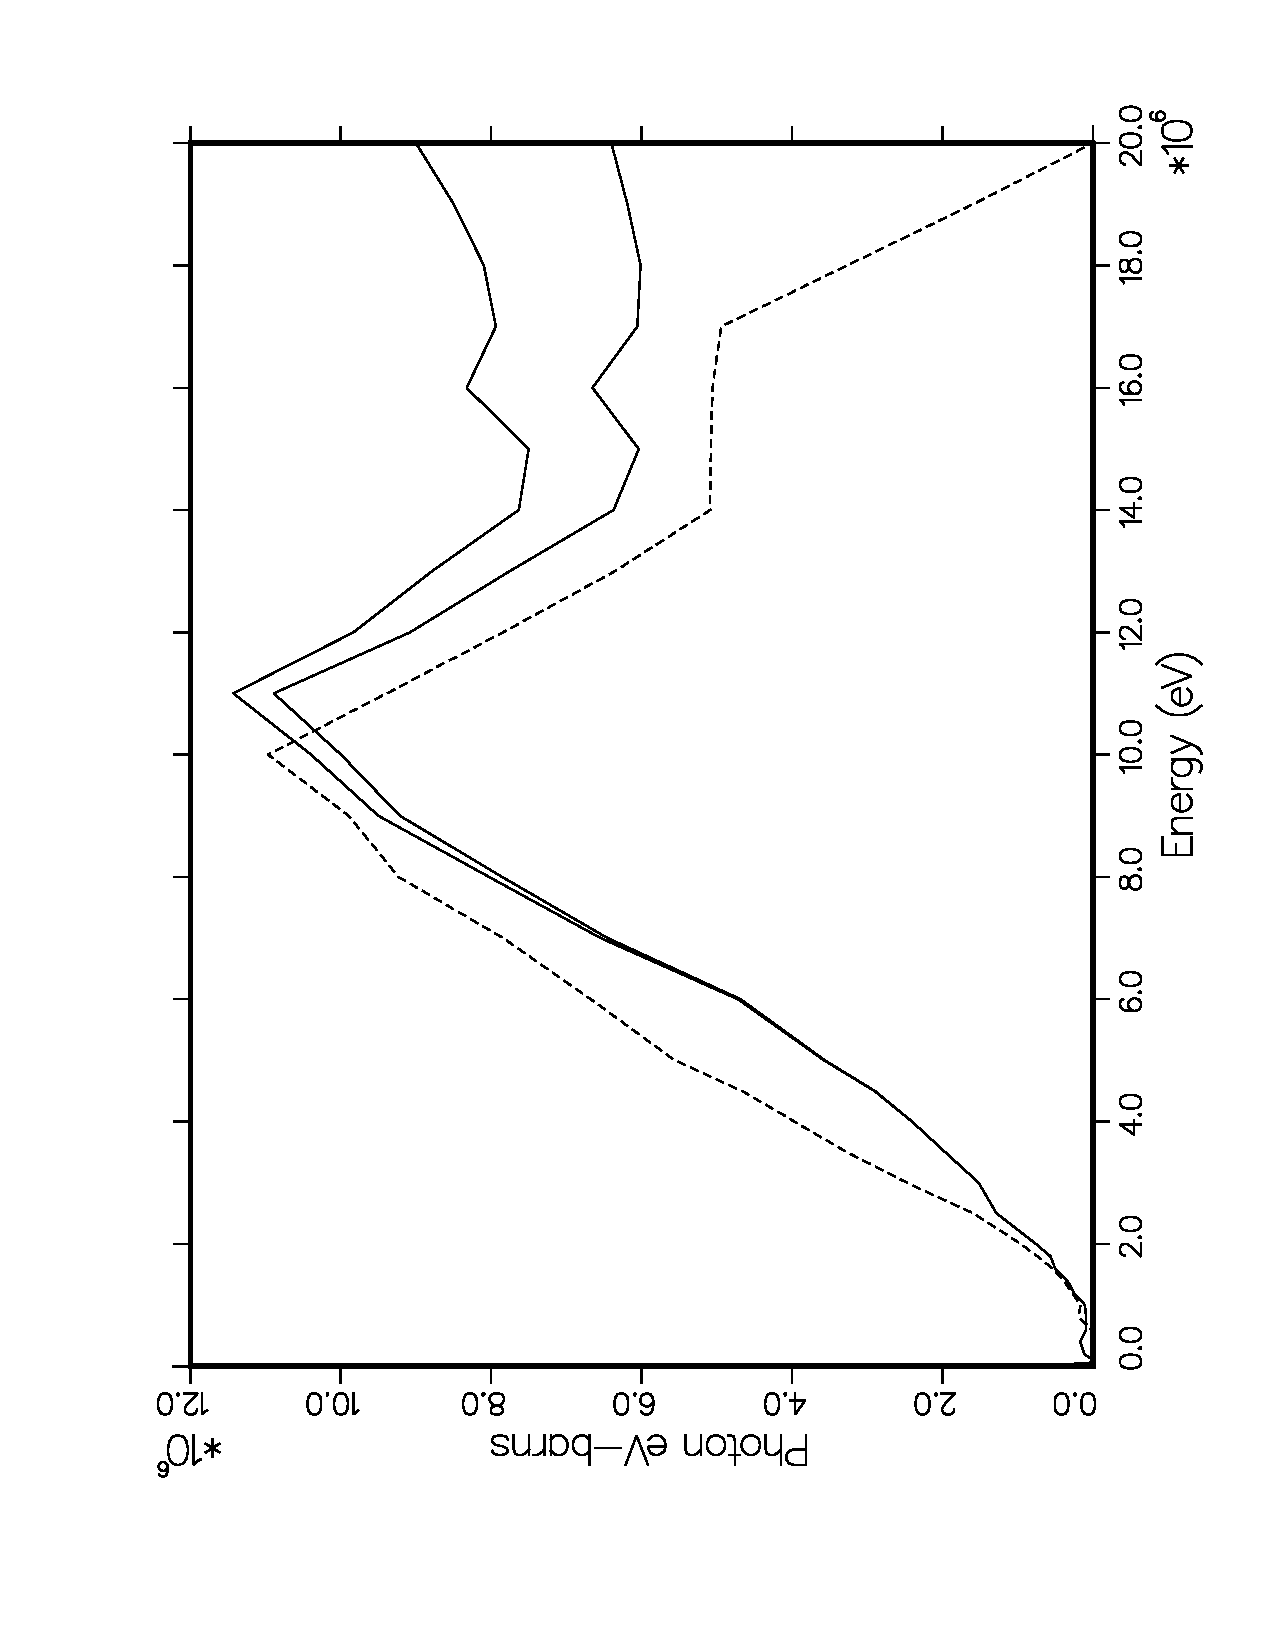
\includegraphics[keepaspectratio,height=3.5in, angle=270]{figs/heatr4ack}
\caption[Total photon energy production and kinematic limits for $^{55}$Mn]
{Example of a plot comparing the total photon energy production for
  $^{55}$Mn from ENDF/B-V.1 (dashed) with the kinematic limits (solid).}
\label{he4}
\end{figure}

The last part of a full HEATR output listing is a tabulation of
the computed KERMA and damage coefficients on the normal coarse
energy grid.  Columns are provided for the total KERMA and
for each of the partial KERMA results requested with \cword{mtk}
values in the user's input.  If kinematic checks were requested,
the check values are written just above and below the corresponding
partial KERMA values.  In addition, \cword{low} and \cword{high}
messages are written just above or just below the kinematic limits
in every column where a significant violation of the limits occurs.
Caution: if summation reactions (MT=3, MT=4) were used to define
the photon production over some parts of the energy range, the
partial KERMA results may not make sense at some energies.  For
example, consider the common pattern in ENDF/B-V where MT=102
is used for capture at low energies, but at higher energies, it
is set to zero, and the capture contribution is included in MT=3
(nonelastic).  Clearly, the partial KERMA MT=402 doesn't make
sense above this breakpoint.  The following example shows part
of the final KERMA listing for ENDF/B-V.1 $^{55}$Mn.  The
damage column was removed and the columns compressed to fit
on the printed page.

\newpage
\small
\begin{ccode}

final kerma factors
          e          301          302          303          402          443

        min   1.2400e-04   3.7775e-06   1.2022e-04   1.2022e-04
 1.0000e-05   4.0068e+05   3.7775e-06   4.0068e+05   4.0068e+05   4.0068e+05
        max   3.3820e+05   3.7775e-06   3.3820e+05   3.3820e+05
                high                      high         high

  ...

        min   3.2373e+04   2.3497e+04   8.8759e+03   4.1114e+01
 6.0031e+05   1.0017e+05   2.3497e+04   7.6673e+04   2.9899e+04   3.2375e+04
        max   3.2375e+04   2.3497e+04   8.8781e+03   4.3366e+01
                high                      high         high

                 low                       low
        min   7.3041e+04   5.9403e+04   1.3638e+04   4.4748e+01
 8.0182e+05  -2.4355e+04   5.9403e+04  -8.3758e+04   2.4987e+04   7.3043e+04
        max   7.3043e+04   5.9403e+04   1.3640e+04   4.6676e+01
                                                        high

                low                       low
        min   9.8973e+04   7.7075e+04   2.1898e+04   4.7777e+01
 1.0000e+06   3.7682e+04   7.7075e+04  -3.9393e+04   2.1917e+04   9.8974e+04
        max   9.8974e+04   7.7075e+04   2.1900e+04   4.9509e+01
                                                        high

                low                       low
        min   1.1397e+05   7.7800e+04   3.6168e+04   4.9760e+01
 1.2000e+06   9.5321e+04   7.7800e+04   1.7521e+04   1.9482e+04   1.1397e+05
        max   1.1397e+05   7.7800e+04   3.6169e+04   5.1335e+01
                                                        high

                low                       low
        min   1.4632e+05   1.0192e+05   4.4402e+04   5.3005e+01
 1.4000e+06   9.8251e+04   1.0192e+05  -3.6667e+03   1.8208e+04   1.4632e+05
        max   1.4632e+05   1.0192e+05   4.4403e+04   5.4511e+01
                                                        high

  ...

        min   2.3650e+05   1.6907e+05   6.7426e+04   1.7607e+02
 1.9000e+07   7.1384e+06   1.6907e+05   6.9693e+06   1.3503e+04   2.5435e+06
        max   2.5435e+06   1.6907e+05   2.3744e+06   1.7939e+02
                high                      high         high

        min   2.4001e+05   1.8261e+05   5.7406e+04   1.4423e+02
 2.0000e+07   9.2369e+06   1.8261e+05   9.0543e+06   1.0908e+04   2.8385e+06
        max   2.8385e+06   1.8261e+05   2.6559e+06   1.4701e+02
                high                      high         high

\end{ccode}
\normalsize

The following subsection discusses how to analyze the ``check''
output of HEATR in order to diagnose energy-balance errors in
ENDF-format evaluations.  The examples are drawn from ENDF/B-V
testing\cite{ebal}.  In general, results like these are less likely to occur
in modern evaluations.

\subsection{Diagnosing Energy-Balance Problems}
\label{ssHEATR_EB_Prob}

The analysis should start with MT=102, because if it is wrong, the
guarantee of energy conservation  for large systems breaks
down.  If the display for MF=12, MT=102 shows messages of the form
``\cword{--- pc}'', there may be a problem.  If these messages only
show up at the higher energies, and if the size of the error
increases with energy, it is probable that the evaluator has
used a thermal spectrum over the entire energy range (this is
very common).  Of course, the total photon energy production
from radiative capture should equal

\begin{equation}
   \frac{A}{A+1}E+Q\,\,,
\end{equation}

\noindent
where the rest of the total energy $E{+}Q$ is carried away by
recoil.  If only a thermal spectrum is given, the $E$ term is
being neglected, and errors will normally appear above about
1 MeV.  The $E$ term can be included in evaluations that use
tabulated data by giving $E$-dependent spectra in File 15; and it
can be included for evaluations that use discrete photons
by setting the ``primary photon'' flags in File 12
properly.  In practice, the capture cross sections above 1 MeV
are often comparatively small due to the $1/v$ tendency of
capture, and the errors introduced by
neglecting the $E$ term can be ignored.

If the MT=102 errors show up at low energies, there is probably
an error in the average photon yield from File 12, in the
average energy computed from File 15, or both.  In the
$^{55}$Mn case shown above, the yield had been incorrectly
entered.  In addition, the spectrum didn't agree with the
experimental data because the bin boundaries were shifted.
Each case must be inspected in detail to find the problems.

The next common source of energy-balance errors in ENDF files
arises from the representation used for inelastic scattering.
Typically, the neutron scattering is described in detail using
up to 40 levels for the (n,n$'$) reaction.  However, the photon
production is often described using MF=13/MT=3 or MF=13/MT=4 and
rather coarse energy resolution.  As a result, it is possible
to find photons for (n,n$_1$) being produced for incident
neutron energies slightly below the MT=51 threshold!  These
photons would lead to a spike of negative KERMA factors.  A
more common effect of the coarse grid used for photon production
is to lead to an underestimate or overestimate of the photon
production by not following the detailed shape of the inelastic
cross section.  The HEATR ``kinematic KERMA'' is correct in
this range since only two-body reactions are active.  Therefore,
a plot of MT=301 and MT=443 on the same frame normally shows
these effects in detail.  Fig.~\ref{he5} is an example of such
a plot.

\begin{figure}[b]\centering
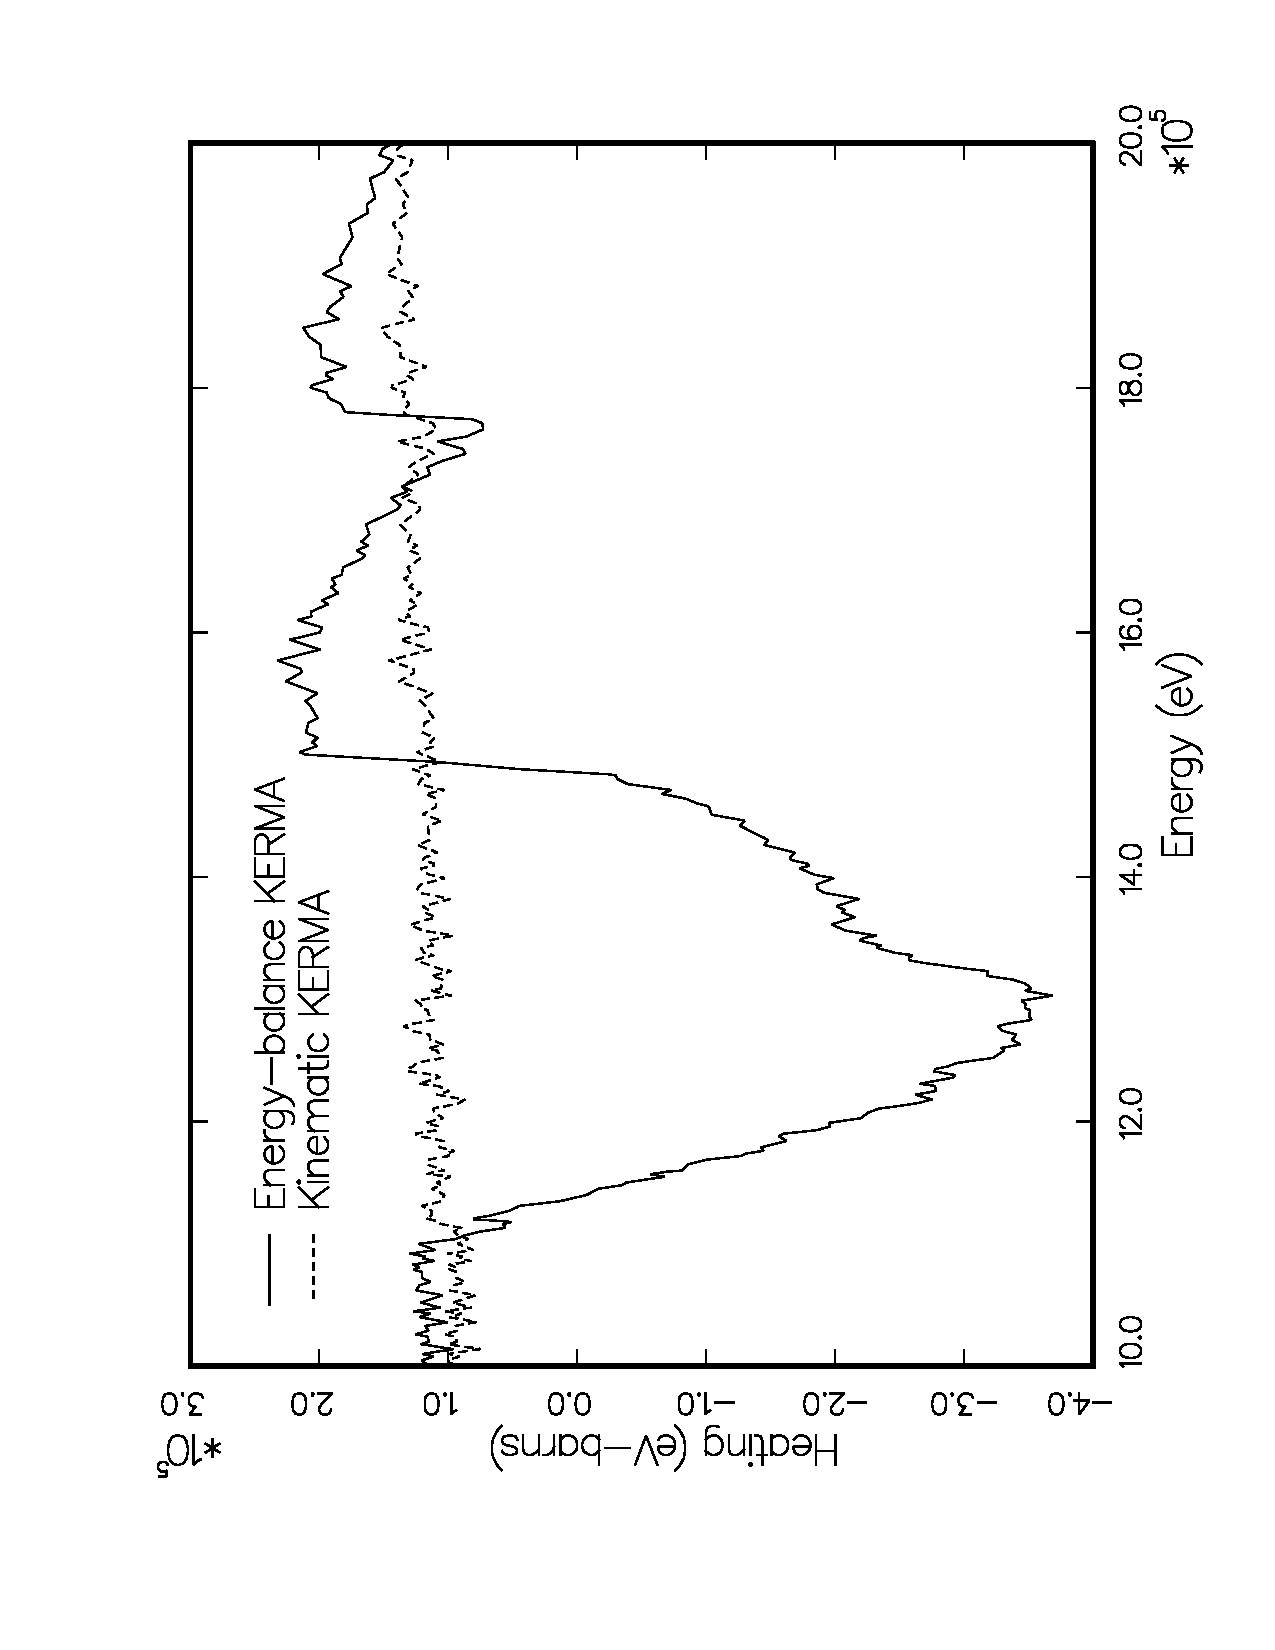
\includegraphics[keepaspectratio,height=3.5in, angle=270]{figs/heatr5ack}
\caption[MT301 and MT443 for $^{59}$Co]{Comparison of MT=301 with
 MT=443 for the region of the discrete-inelastic thresholds for $^{59}$Co
 from ENDF/B-V.2.  Note the large region of negative KERMA.  The best way
 to remove this kind of problem is by using yields in File 12, MT=51, 52, 53,
 \ldots to represent the photon production.}
\label{he5}
\end{figure}

Fig.~\ref{he6} shows both the inelastic cross section
from File 3 and the photon production cross section from File 13
to demonstrate the mismatch in the energy grids that contributes
to the energy-balance errors.  These kinds of errors are best
removed by changing to a representation that uses File 12 to
give photon production yields for the separate reactions MT=51,
MT=52, etc.  This representation makes full use of the File 3
cross sections, and as long as each section of File 12
conserves energy, the total inelastic reaction is guaranteed to
conserve energy, even at the finest energy resolution.

\begin{figure}[t]\centering
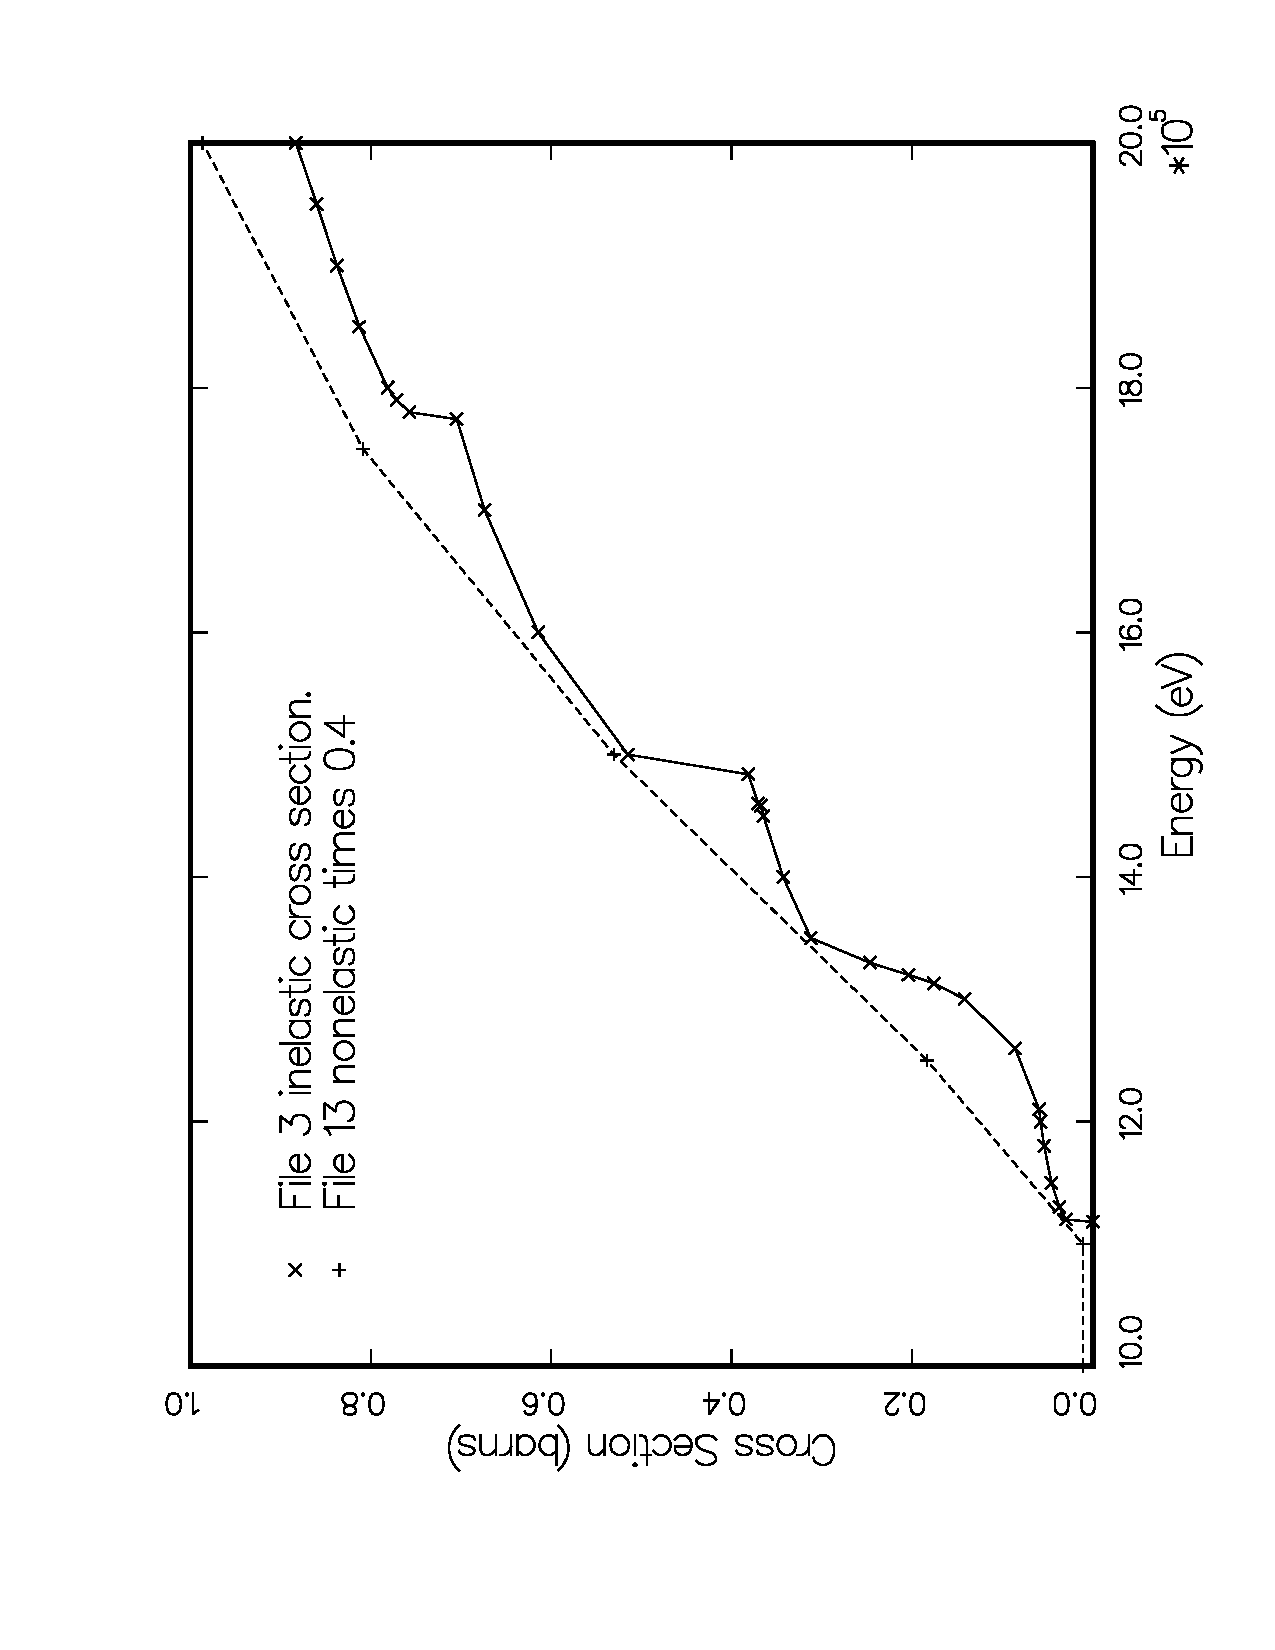
\includegraphics[keepaspectratio,height=3.2in, angle=270]{figs/heatr6ack}
\caption[Example of File 3 and File 13 energy grid mis-match]{Plot
 showing  the mismatch between the energy grids used for File 3
 and File 13 in the region of the thresholds for discrete-inelastic
 scattering levels for the case shown in Fig.~\ref{he5}. The cross
 and ex symbols show the actual grid energies in the evaluation.}
\label{he6}
\end{figure}

\begin{figure}[b]\centering
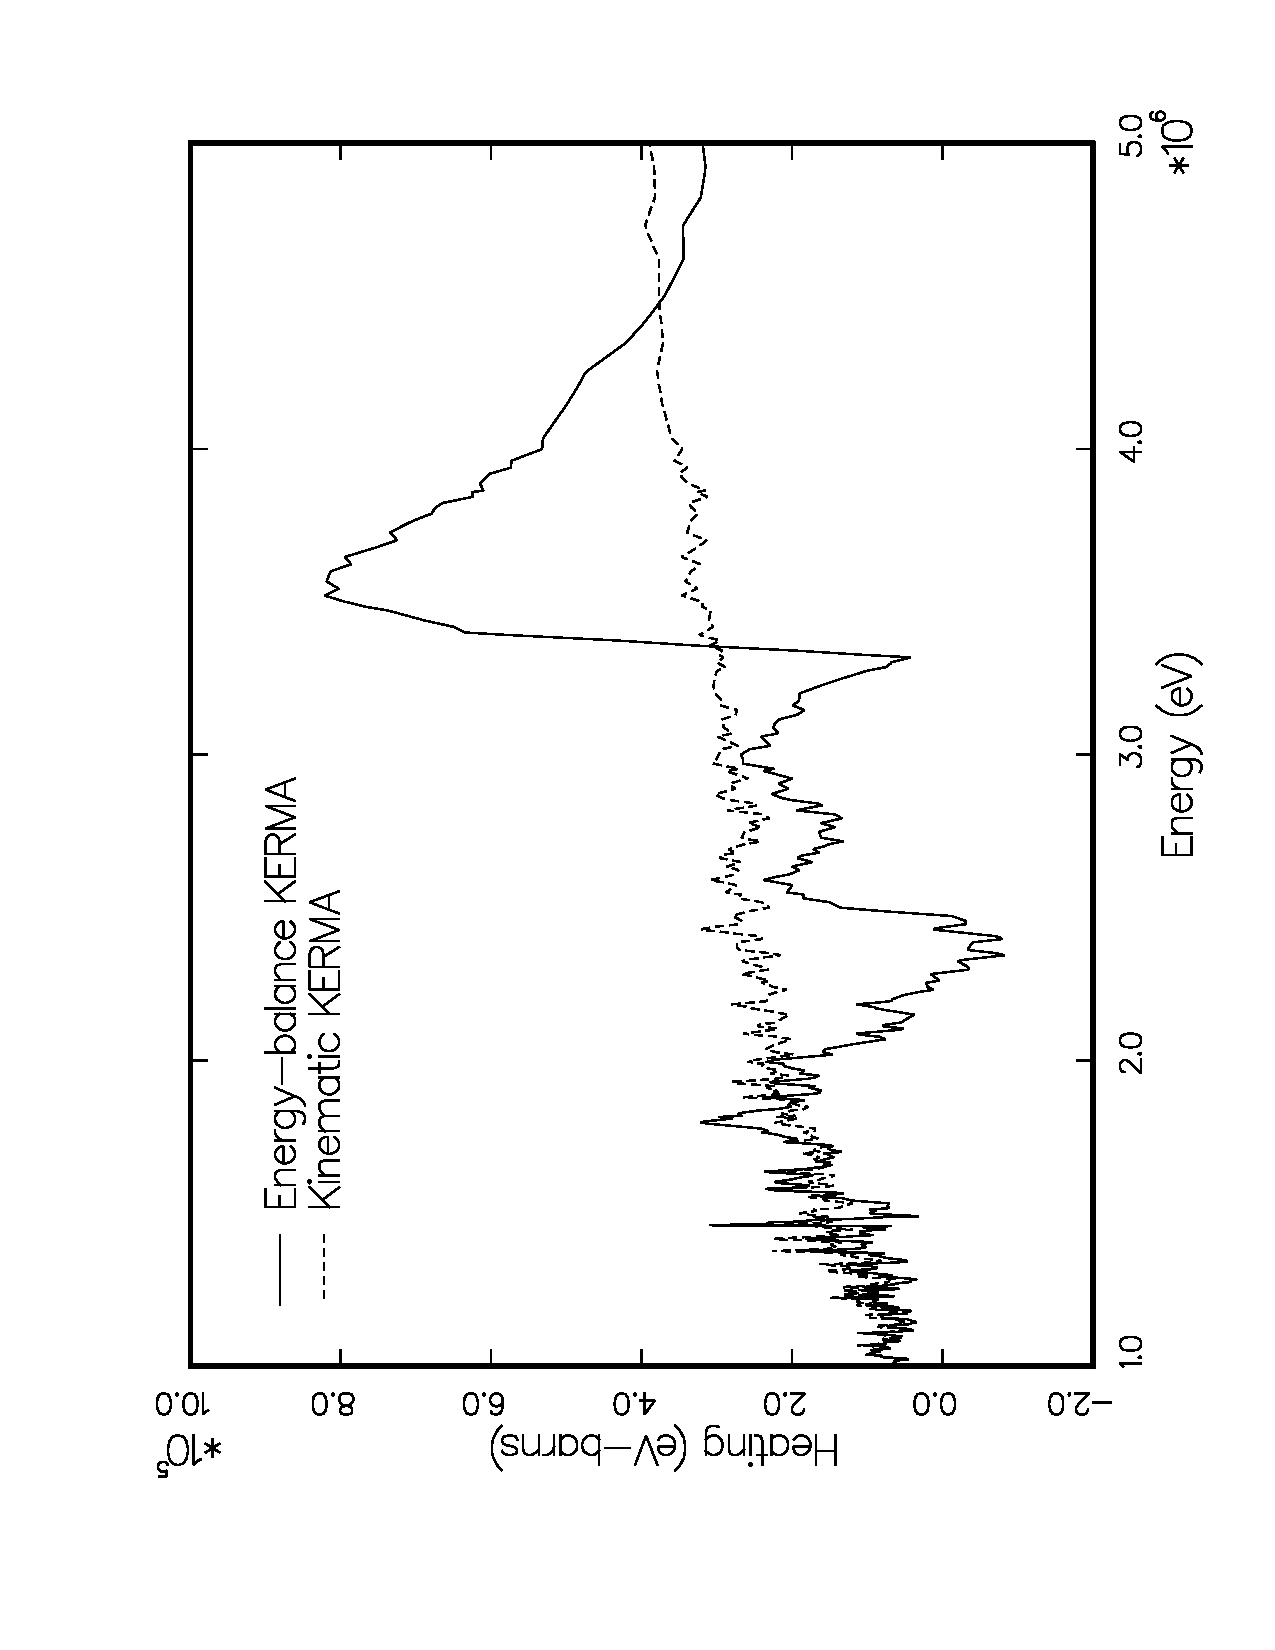
\includegraphics[keepaspectratio,height=3.2in, angle=-90]{figs/heatr7ack}
\caption[Example of energy-balance problems]{Typical energy-balance
 problems between points where balance is satisfied.  Discrete photons
 were used below about 2 MeV, and energy balance is reasonably good
 there.  The energy points in MF=13 for the continuum part are at 2, 3, and
 5 MeV, and the balance is also good at those energies.  Clearly, a grid
 in File 13 that used steps of about 0.25 MeV between 2 and 4 MeV would
 reduce the size of the deviations substantially and remove the negative
 KERMA factors.}
\label{he7}
\end{figure}

A method that is frequently used by evaluators of photon production
files is to select a number of nonelastic photon spectra on a
fairly coarse incident-energy grid using theory or experiment,
and then to readjust the photon yield on this energy grid so as
to conserve energy at each grid point.  However, the results do
not, in general, conserve energy at intermediate points.  If a
very coarse energy grid is used for File 13, quite large
deviations between MT=301 and MT=443 can result.  Fig.~\ref{he7}
shows such a case.  The solution to this kind of violation of
energy balance is to add intermediate points in Files 13 and 15
until the magnitude of the deviations is small enough for
practical calculations.

Especially large energy-balance errors of this type are caused
by interpolating across the minimum formed by the decreasing
capture heating and the increasing inelastic heating.
Fig.~\ref{he8} shows a dramatic example using a photon energy
production comparison.

\begin{figure}[bp]\centering
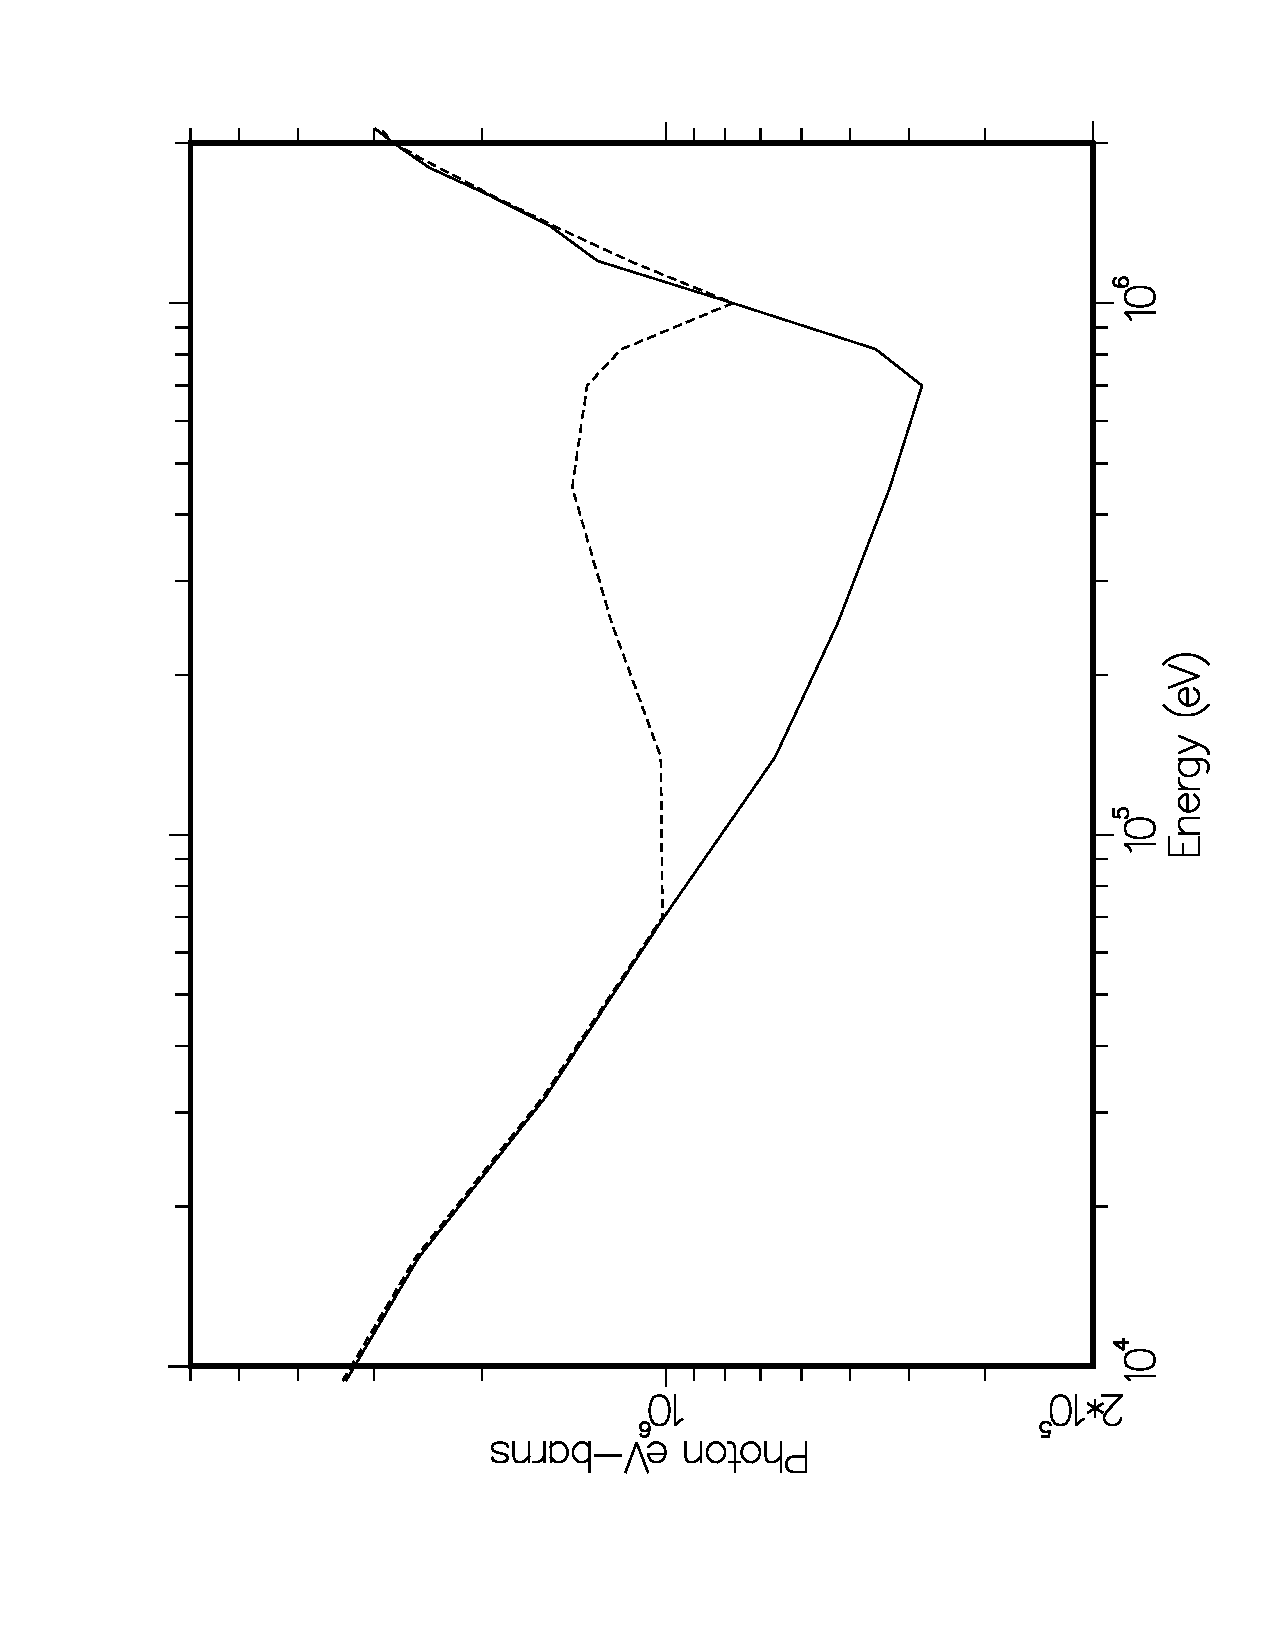
\includegraphics[keepaspectratio,height=3.5in, angle=270]{figs/heatr8ack}
\caption[Computed photon energy production and kinematic values]{Computed
 photon energy production (dashed) compared with the kinematic value
 (solid) for $^{93}$Nb from ENDF/B-V.  The original File 13 has grid points
 at 100 keV and 1 MeV.  Interpolating across that wide bin gives a photon
 production rate that is much too large for energies in the vicinity of a few
 hundred keV.  This will result in a large region of negative heating
 heating numbers.  Since this is just the region of the peak flux in a fast
 reactor, niobium-clad regions could be cooled instead of heated!}
\label{he8}
\end{figure}

For energies above the threshold for continuum reactions like
(n,n$'$) or (n,2n), it is difficult to use the results of the
kinematic checks to fix evaluations.  The representation of
Eqs.~\ref{contin} and \ref{contin2} for continuum inelastic
scattering is very rough.  Comparison to other more accurate
methods suggests that a CM formula would be better
here\cite{advanced}, even though the ENDF file says ``lab.''
Most other reactions give very wide low and high limits.  Two
exceptions are (n,2n) and (n,3n).  If they dominate the cross
section, the kinematic limits will be fairly close together.
In the 14 MeV range, energy errors could be in the photon data,
the neutron data, or both.  The best way to eliminate balance
errors is to construct a new evaluation based on up-to-date
nuclear model codes.

\subsection{Coding Details}
\label{ssHEATR_details}

The main subroutine is \cword{heatr}\index{heatr@{\ty heatr}}, which is
exported by module \cword{heatm}\index{modules!heatm@{\ty heatm}}.
It starts by reading the user's input and locating the desired
material on the PENDF\index{PENDF} file.  The main loop is over
temperature.  For each temperature, a check is made to see if
the user provided a value for the damage displacement energy.
If not, a default value is provided.  Next, \cword{hinit}
\index{hinit@{\ty hinit}} is called to examine the directory.  Flags
are set if MF=12 or 13 is present, if MT=18 or 19 is used, and if
MT=458 is present (see \cword{mgam}, \cword{mt19}, and \cword{mt458}).
The flags \cword{mt103}, \cword{mt104}, \cword{mt105}, \cword{mt106}
and \cword{mt107} are set if the corresponding particle production
levels are present.  The MT numbers used for the levels depend on
whether the input file used version 6 format or one of the earlier
formats.  For example, \cword{mt103} is set if MT=600-649 is found
for ENDF-6 data, or if MT=700-719 is found for earlier versions.
The code also checks to see if the corresponding angular distribution
data are present (see \cword{nmiss4}).  If any are not present, the
code will assume they are isotropic.  Note that \cword{hinit} also
collects a list of the File 6 MT numbers in \cword{mt6(i6)}.
For fissionable materials, the delayed fission energy values
are retrieved from MF=1/MT=458, and the correction, \cword{qdel}, is
computed for later use when calculating the heating from prompt
fission.

The next step in \cword{hinit} is to make a copy of File 6 on a
scratch file (if any sections of File 6 were found).  While doing
this, it searches through the subsections for each reaction
accumulating the ZA residual remaining after each particle is
given.  If it comes to the photons (\cword{zap}=0), which should
be last, and there is still a ZA residual left, then it concludes
that there is no subsection describing the residual.  It loads
a value into \cword{mt6no(ii6)} that is the index to the
subsection that the recoil should have followed had it been
present.  If it comes to the end of the subsection list without
finding photons and still has a ZA residual, it sets \cword{mt6no(ii6)}
to \cword{nk}; that is, the residual missing should follow the last
subsection.  In either case, the routine prints out messages
about ``photon recoil correction'' or ``one-particle recoil
approximation.''

Finally, \cword{hinit} makes a standardized copy of the ENDF tape
using \cword{hconvr}\index{hconvr@{\ty hconvr}}, and it also saves
the grid of the total cross section (MT=1) on the \cword{loada/finda}
scratch file that will be used to accumulate the KERMA factors,
damage, and kinematic checks (if requested).  Note also \cword{mt303},
which tells which of the requested edits is for nonelastic heating,
MT=303.  This is used later for writing out the photon energy
production check.

Now \cword{nheat}\index{nheat@{\ty nheat}} is called.   Its basic
function is to loop over the ``nonredundant'' reactions in File 3,
and to accumulate the corresponding contributions to the partial
heating and partial damage values into the appropriate elements
of the \cword{c} array on the \cword{loada/finda} file.  Redundant
reactions are reactions that duplicate or include effects that
can be obtained from another MT number.  They are determined using
a set of \cword{if} statements just after the entry to the reaction
loop at statement number 105.  The structure of the \cword{c} array
depends on whether kinematic checks are being accumulated or not
and whether photon production files are present.  If neither
occurs, the structure has \cword{npk}+1 elements as follows:

\begin{center}
\begin{tabular}{cl}
Element & Contents \\ \hline
\cword{1} & energy \\
\cword{2} & total heating \\
\cword{3} & value for first partial \\
$\cdots$ & \\
\cword{npk}+1 & value for last partial \\ \hline
\end{tabular}
\end{center}

\noindent
where \cword{npk} is the number of partial KERMA or damage
values being accumulated, including the total.
If checks are being accumulated, the \cword{c} array has the
following 3*\cword{npk}+1 elements:

\begin{center}
\begin{tabular}{cl}
Element & Contents \\ \hline
\cword{1} & energy \\
\cword{2} & total heating \\
\cword{3} & value for first partial \\
$\cdots$ & \\
2+\cword{npk} & lower kinematic limit for total \\
3+\cword{npk} & lower kinematic limit for first partial \\
$\cdots$ & \\
2+2*\cword{npk} & upper kinematic limit for total \\
3+2*\cword{npk} & upper kinematic limit for first partial \\
$\cdots$ & \\
3*\cword{npk}+1 & upper kinematic limit for last partial \\ \hline
\end{tabular}
\end{center}

\noindent
If photon production files are present in the evaluation, the total
length of the \cword{c} array increases by the following three
words (\cword{len} is the old length from above plus three):

\begin{center}
\begin{tabular}{cl}
Element & Contents \\ \hline
\cword{len}-2 & photon capture correction \\
\cword{len}-1 & total photon eV-barns \\
\cword{len} & total energy yield for ``subtot'' \\ \hline
\end{tabular}
\end{center}

Back inside the loop over nonredundant reactions, subroutine
\cword{gety1}\index{gety1@{\ty gety1}} is initialized for this
reaction.  The code checks to see if this section uses File 6
for its distributions; if so, it arranges to make multiple passes
through the reaction's energy grid, one pass for each subsection
of the MF=6 section, and perhaps one additional pass to synthesize
the missing recoil subsection.  It is now possible to select the
appropriate $Q$-value and particle yield, and to initialize the
appropriate calculational routine.  This routine will be
\cword{sixbar}\index{sixbar@{\ty sixbar}} for all reactions
described in File 6, \cword{disbar}\index{disbar@{\ty disbar}} for
two-body reactions using File 4 (including charged-particle
reactions in the 600 or 700 series of MT numbers),
\cword{conbar}\index{conbar@{\ty conbar}} for continuum reactions
represented using File 5, and \cword{capdam}\index{capdam@{\ty capdam}}
for the neutron disappearance reactions (MT=102, 103, {\it etc.})
and the charged-particle continuum reactions from the 600 or 700
series of MT numbers.  The last step before beginning the energy
loop for this reaction is to call \cword{indx}\index{indx@{\ty indx}},
which determines which element of the \cword{c} array is to receive
the heating or damage contribution from this reaction (see below).

The energy loop in \cword{nheat}\index{nheat@{\ty nheat}} goes
through statement number 190.  For each energy,
\cword{finda}\index{finda@{\ty finda}} is called to retrieve the current
values for the energy [see \cword{c(1)}] and the partial heating
and damage values as accumulated so far.  On the first pass
through the scratch file, the list of energies to be used for
printing information on the listing is established in
\cword{elist} using a few \cword{if} statements based on the
range of the energy variable \cword{e}.  For each energy, the
corresponding cross section is retrieved using
\cword{gety1}\index{gety1@{\ty gety1}} and
the appropriate $\overline{E}$ and damage numbers are computed
by calling \cword{getsix}\index{getsix@{\ty getsix}},
\cword{disbar}\index{disbar@{\ty disbar}},
\cword{conbar}\index{conbar@{\ty conbar}}, or
\cword{capdam}\index{capdam@{\ty capdam}}.  The heating contribution
is computed from the appropriate formula, and the heating and damage
numbers are summed into the \cword{c} array at location \cword{index}.
If requested, the kinematic limits on the heating are computed and
summed into the \cword{c} array at \cword{index}+\cword{npk} and
\cword{index}+2*\cword{npk}.  The completed results for this energy and
reaction are written out onto the \cword{loada/finda} scratch file,
and the energy loop is continued.

When the energy loop is complete, the subroutine jumps to the
next section (or subsection in the case of File 6) and repeats the
entire energy loop for that reaction (or particle from File 6).

Subroutine \cword{indx}\index{indx@{\ty indx}} is used to
select what element of the \cword{c} array is to receive the
heating or damage contribution for a section with a particular
MT number.  The meaning of each element of the \cword{c} array
is obtained from the \cword{mtp} array.  Normally, a reaction
MT contributes to the partial heating element with
\cword{mtp(i)}=MT+300.  But it can also contribute to
several other elements of \cword{c}, such as nonelastic
(MT=303), inelastic (MT=304), etc.  Therefore, \cword{indx}
returns the count of reactions contributed to by \cword{mt}
in \cword{nmt} and the indexes for the \cword{c} array in
\cword{imt(nmt)}.

Subroutine \cword{capdam}\index{capdam@{\ty capdam}}
is used to compute the damage energy for neutron capture
(or disappearance) reactions; that is, for MT=102, 103,
etc.  On the initialization entry (\cword{ee}=0.0), the
routine sets up various kinematics parameters, such as \cword{zx}
and \cword{ax} to describe the outgoing particle, and initializes
\cword{df}.  In order to save time, the routine only calculates the
damage on a grid that increases by steps of 10\%.  Intermediate
values are obtained by interpolation (see \cword{el}, \cword{daml},
\cword{en}, and \cword{damn}).  The values at the grid points
are computed using

\begin{equation}
   D\left(\frac{E}{A+1}\right)
    +D\left(\frac{1}{2M_Rc^2}\left[\frac{AE}{A+1}+Q\right]^2\right)
\end{equation}

\noindent
for radiative capture (the corrections for multiple photon emission
will be made later), or using Eq.~\ref{damint} with $E_R$
from Eq.~\ref{npart} and a 4-point Gauss-Legendre
\index{Gauss-Legendre quadrature} quadrature.  The angular
distribution for particle emission is taken to be isotropic.

Subroutine \cword{disbar}\index{disbar@{\ty disbar}} is used by
\cword{nheat} to compute the average secondary energy and damage
energy for elastic scattering (MT=2), discrete-inelastic scattering
(MT=51-90), or discrete-level particle production (MT=600-648,
650-698, etc. for ENDF/B-VI or ENDF/B-VII, or MT=700-717,
720-737, etc. for earlier versions).  It starts by initializing
\cword{hgtfle}\index{hgtfle@{\ty hgtfle}} (which is very similar to
\cword{getfle}\index{getfle@{\ty getfle}} in the GROUPR module),
determining kinematic parameters like \cword{awp} (the mass ratio
to the neutron for the emitted particle), and initializing
\cword{df}\index{df@{\ty df}}.  In order to save time, it only
computes the heating and damage on a grid based on steps by a
factor of 1.1 and the \cword{enext} values from \cword{hgtfle}.
On a normal entry, it interpolates between these values (see
\cword{el}, \cword{cl}, \cword{daml}, \cword{en}, \cword{cn}, and
\cword{damn}).  When the desired \cword{ee} exceeds \cword{en},
the old high values are moved down to the low positions, and new
high values are calculated.  The calculation of \cword{cn}
follows Eq.~\ref{enb}.  The calculation of \cword{damn} uses
Eq.~\ref{damint} with a 20-point Gauss-Legendre quadrature
(see \cword{nq}, \cword{qp}, and \cword{qw}).

Function \cword{df}\index{df@{\ty df}} is used to compute the
damage partition function given in Eq.~\ref{robinson}.  The
constants that depend on the recoil atom or particle type and
lattice type (see \cword{zr}, \cword{ar}, \cword{zl}, \cword{al})
are computed in an initialization call with \cword{e}=0.0.  Thereafter,
it can be called with any other value of \cword{e}.

Similarly, \cword{conbar}\index{conbar@{\ty conbar}} computes
the average secondary energy and damage energy for continuous
distributions described in File 5.  Analytic representations use
simple formulas coded into \cword{anabar}\index{anabar@{\ty anabar}}
or a combination of adaptive and Gaussian quadrature in
\cword{anadam}\index{anadam@{\ty anadam}}.  Tabulated data are
interpolated from the File 5 table using
\cword{tabbar}\index{tabbar@{\ty tabbar}} or integrated using
trapezoidal and Gaussian quadratures in
\cword{tabdam}\index{tabdam@{\ty tabdam}}.  As usual, the routine
is initialized by calling it with \cword{e}=0.0.  The
secondary-particle yield is either chosen from the MT number,
or \cword{hgtyld}\index{hgtyld@{\ty hgtyld}} is initialized.  The
desired section of File 5 is located on the input ENDF tape, and the
kinematic constants are computed.  The reactions
with MT=22, 28, 32, 33, and 34 will be treated using the
\cword{capdam}\index{capdam@{\ty capdam}} method; if
\cword{mtd} has one of these values (see \cword{mtt}),
\cword{capdam} is initialized.  As is the case for
\cword{getsed}\index{getsed@{\ty getsed}} in the
\hyperlink{sGROUPRhy}{GROUPR}\index{GROUPR}
module, this routine can handle some sections of File 5 that contain
multiple subsections, but the analytic subsections must come
first.  As each analytic subsection is read, appropriate data
are stored in in the external array \cword{c} using pointers
saved in the array \cword{loc}.  Only the first energy is read
and stored for a tabulated subsection (\cword{lf}=1).  The
idea is to have only two energy values in memory at a time
in order to save storage; the second subsection will be read
during the first normal entry to the subroutine.  The final
step in the initialization pass is to initialize
\cword{df}\index{df@{\ty df}}.  For a normal entry into
\cword{conbar}\index{conbar@{\ty conbar}}, the energy-dependent
fission yield is retrieved, if needed, and the loop over
subsections is entered.  Each subsection in File 5 starts
with a fractional-probability record.  The desired value
for energy \cword{e} is computed by interpolation using the
standard \hyperlink{sNJOYhy}{NJOY} utility routine
\cword{terpa}\index{terpa@{\ty terpa}}.
For analytic subsections, the routine uses
\cword{anabar}\index{anabar@{\ty anabar}} to compute
$\overline{E_n}$, and \cword{anadam} or
\cword{capdam}\index{capdam@{\ty capdam}} to
compute the damage energy. Note that in order to save time,
\cword{anadam} is only calculated on a fairly coarse grid
based on steps by a factor of 1.5.  The intermediate values
are obtained by interpolation using
\cword{terp1}\index{terp1@{\ty terp1}}.  For
tabulated subsections, \cword{ebar} and \cword{dame} values
are normally obtained by interpolation (see \cword{elo},
\cword{flo}, \cword{dlo}, \cword{ehi}, \cword{fhi}, and
\cword{dhi}).  However, for the first entry, or whenever
\cword{e} reaches \cword{ehi}, the high data are moved into
the low positions, new high data are read from the File 5
subsection, and the values for heating and damage
are computed at \cword{ehi} using
\cword{tabbar}\index{tabbar@{\ty tabbar}} and
either \cword{tabdam}\index{tabdam@{\ty tabdam}} or
\cword{capdam}\index{capdam@{\ty capdam}}.

Subroutine \cword{hgtyld}\index{hgtyld@{\ty hgtyld}} is
similar to \cword{getyld}\index{getyld@{\ty getyld}} in the
\hyperlink{sGROUPRhy}{GROUPR}\index{GROUPR}
module.  It finds the required section on
the ENDF tape and reads the entire LIST or TAB1 record into
memory.  On normal entries, it either computes the yield using the
polynomial formula with constants from the LIST record, or
it uses \cword{terpa}\index{terpa@{\ty terpa}} to interpolate for
the yield in the TAB1 data.

Subroutine \cword{anabar}\index{anabar@{\ty anabar}}
is used to compute the average energy for a neutron described
by an analytic subsection of File 5.  The simple formulas
used are tabulated in the ENDF format manual\cite{ENDF102}.
Similarly, \cword{anadam}\index{anadam@{\ty anadam}} is used to
compute the damage energy for an analytic subsection of File 5.
Only LF=9 (the Simple Maxwellian Distribution) is supported; the
routine returns zero for other laws.  Note that a statement function
is defined to compute the secondary energy distribution for
this law (see \cword{sed}).  For each incident energy, the
spectrum temperature \cword{theta} is retrieved using
\cword{terpa}, and an adaptive integration stack is
initialized with points at four secondary energies,
namely, 1., $.5(E{-}U)$, $\theta$, and $E{-}U$, where $U$ is
a parameter that sets the maximum possible value of $E'$.
The adaptive procedure proceeds to solve Eq.~\ref{f5dam}
by subdividing this starting grid until trapezoidal integration
can be used on each panel.  The inner integral over emission
cosine $\mu$ is performed using a 4-point Gauss-Legendre
quadrature for each point on the adaptive grid.  The
function \cword{sed} is used to compute $g(E')$, and
\cword{df}\index{df@{\ty df}} is used to compute the
partition function.

Subroutine \cword{tabbar}\index{tabbar@{\ty tabbar}}
is used to compute the average energy of the emitted neutron
for a tabulated subsection of File 5.  It can also be used
for a tabulated subsection of File 6.  This option is
flagged by \cword{law} negative.  The trick is to set
the ``stride'' or ``cycle'' through the file to be larger
than 2 (see \cword{ncyc}).  The angular part of the
$g(E{\rightarrow}E')$ table is skipped, and only the $E'$ and
$g$ values are retrieved.  For File 5, this routine only works
for laws 1 and 5; others cause a fatal error message to be
issued.  In both of these cases, the integral over $E'$ needed
to compute the average energy is done analytically for each
panel in the input data using a different formula for each
interpolation scheme \cword{int}.

Subroutine \cword{tabdam}\index{tabdam@{\ty tabdam}}
is used to compute the damage energy for a tabulated subsection
of File 5.  The integration that is needed is given in
Eq.~\ref{f5dam}.  The energy grid of the tabulation
is assumed to be good enough to allow trapezoidal
integration to be used for $E'$, and a 4-point Gauss-Legendre
quadrature is used for $\mu$.

Subroutine \cword{sixbar}\index{sixbar@{\ty sixbar}}
is used to compute charged-particle average energy and
damage energy represented by using a subsection of File 6.
As is common with NJOY subroutines, \cword{sixbar} is
initialized by calling it with \cword{e}=0.0.  The initialization
path is controlled by \cword{j6}, which is the index
to the current subsection in File 6; by \cword{irec},
which is 1 when a recoil response is to be calculated, and
by \cword{jrec}, which tells the routine how to get back to
the next subsection after a recoil calculation.  If this is
not a recoil subsection, the routine jumps to statement 110
and starts reading in the data for the desired subsection.
If it is flagged as a recoil (see \cword{irec}), the routine
backs up to the subsection describing the particle that induced
the recoil and then continues by reading in the data for that
particle.

The first step is to read in the TAB1 record
that contains the particle yield, identity (\cword{zap}
and \cword{awp}), and representation \cword{law}.
If this law describes a two-body recoil distribution, the
routine sets \cword{jrec} for a proper return, sets
\cword{irec} to back up to the corresponding direct emission
subsection, and jumps back to the beginning of the routine
to do the recoil calculation.

When the code finally arrives at statement number 210, it is
ready to start processing the current subsection.  It reads
in the parameters for laws 3 and 6, or the TAB2 record and
the data for the first energy point for the other laws.  With
the data in place, it computes the corresponding values
for mean energy and damage energy using
\cword{getsix}\index{getsix@{\ty getsix}} or
\cword{tabsq6}\index{tbsq6@{\ty tabsq6}} and returns.

In the special case where the section contains only a single
subsection that describes a neutron, the data stored in
memory will be the data for that subsection, and the
subroutine \cword{tabbar}\index{tabbar@{\ty tabbar}} with a
negative value for the law is used to produce the low values.

On a normal entry (\cword{e}$>$0),
\cword{sixbar}\index{sixbar@{\ty sixbar}} checks to
see whether \cword{e} is in the current interpolation range.
If it is, the code jumps to statement number 400.  For the
analytic laws (\cword{law}=3 and \cword{law}=6), it uses
a direct call to \cword{getsix} to compute the mean energy
and damage energy.  For the tabulated laws, it interpolates
for the results using the low and high data (see \cword{elo},
\cword{flo}, \cword{dlo}, \cword{ehi}, \cword{fhi}, and
\cword{dhi}).  On the first entry, or whenever \cword{e}
increases to \cword{ehi}, the code moves the high data to
the low positions, and then it reads in the data for the
next energy and computes a new set of high values for
mean energy and damage using \cword{getsix} or \cword{tabsq6}.

Subroutine \cword{getsix}\index{getsix@{\ty getsix}}
is used to compute the mean energy and damage energy for
one particular incident energy in a subsection of File 6.
The method used depends on the value of \cword{law} and
the reference frame for the subsection.  The first case
in the coding is for \cword{law}=1 with data in the CM system.

This case uses Eqs.~\ref{KofE} and \ref{DofE} with an
adaptive integration over $E'$.  The integration stack is
contained in the arrays \cword{x} and \cword{y}.  It is
primed with \cword{x(2)}=0, and \cword{h6cm} is called to
compute \cword{y(2)} and the next grid point \cword{epnext}.
The first panel is completed by calculating \cword{y(1)} and
\cword{x(1)}=\cword{epnext}.  The panel is then divided in half, and
the midpoint is tested to see if it is within \cword{tol}=0.02
({\it i.e.}, 2\%) of the linearly interpolated value.  If
not, the midpoint is inserted in \cword{x} and \cword{y},
and the new top panel [that is \cword{x(2)}$-$\cword{x(3)}]
is tested.  This continues until convergence is achieved in
the top panel.  The contributions to the heating and damage
are added into the accumulating integrals at statement
number 190, and \cword{i} is decremented so that the process
can be repeated for the next panel down.  When \cword{i}
decreases to one, the current value of \cword{epnext} is
used to start the next higher $E'$ panel.  This loop over
panels continues until the entire $E'$ range has been
integrated.

The next special case is for tabulated distributions that use
$E$, $E'$, $\mu$ ordering in the lab system.  The angular part
is ignored.  A simple loop over the \cword{NEP} points in
$g(E{\rightarrow}E')$ is carried out.  Trapezoidal integration
is used for each panel for both heating and damage (\cword{h}
and \cword{d}).  If \cword{nd}$>$0, the first \cword{nd} entries
are discrete energies, and the values of the integrand at
those energies are added into \cword{h} and \cword{d}.
Finally, \cword{h} and \cword{d} are copied into \cword{ebar}
and \cword{dame}.

The block of coding starting at statement number 450 is used to
compute particle mean energies for the emitted particles from
two-body reactions, or to compute the mean recoil energy for a
two-body reaction (see \cword{irec}$>$0).  The calculation
follows Eq.~\ref{ebar6}.  Note that the kinematic factors
include \cword{awp}, the mass ratio of the emitted particle to
the incident particle.  The parameter \cword{beta} here is
the same as $R$ in Eq.~\ref{beta}.  If the angular
distribution in File 6 is in Legendre form, the heating
and damage integrals are performed using a 20-point
Gauss-Legendre quadrature (see \cword{nq}, \cword{qp},
and \cword{qw}).  If the angular distribution is tabulated
as $f(\mu)$ {\it versus} $\mu$, a trapezoidal integration is used
for both heating and damage.

The final option in \cword{getsix} is for lab distributions
that use $E$, $\mu$, $E'$ ordering.  See Eq.~\ref{llnl}.
The inner integrals are computed using trapezoidal integration.
The outer integral over $\mu$ also uses trapezoidal integration
on the results of the inner integrals for each $\mu$ grid point.

Note that \cword{getsix} has an \cword{irec} parameter in its
calling list.  When this parameter is greater than zero, the
angular distribution is complemented and the charge and mass of
the particle are modified to represent the recoil species.
The value of \cword{irec} is controlled by \cword{sixbar}.

Subroutine \cword{h6cm}\index{h6cm@{\ty h6cm}} is used by
\cword{getsix} to compute the lab distribution
$g(E{\rightarrow}E'_L)$ of Eq.~\ref{transCM}
using the CM data in File 6.  This subroutine uses
\cword{h6dis}\index{h6dis@{\ty h6dis}},
\cword{h6ddx}\index{h6ddx@{\ty h6ddx}} and
\cword{h6psp}\index{h6psp@{\ty h6psp}} to retrieve the CM discrete,
tabulated or phase-space data from the file.  These routines are
basically the same as \cword{f6cm}\index{f6cm@{\ty f6cm}},
\cword{f6dis}\index{f6dis@{\ty f6dis}},
\cword{f6ddx}\index{f6ddx@{\ty f6ddx}}
and \cword{f6psp}\index{f6psp@{\ty f6psp}}.  See
\hyperlink{sGROUPRhy}{GROUPR}\index{GROUPR} for more details.

Subroutine \cword{gheat}\index{gheat@{\ty gheat}}
is used to correct the heating and damage values accumulated
during the pass through the neutron sections.  It loops through
all of the reactions in File 12 and File 13 using two
ENDF-type tapes.  One is the input PENDF tape, which is used
to retrieve cross sections for use with the photon
multiplicities in File 12.  The other is a version of
the input ENDF tape that has been passed through
\cword{hconvr}\index{hconvr@{\ty hconvr}} to put the photon
data in a standard form (see
Chapter \ref{sGROUPR} (\hyperlink{sGROUPRhy}{GROUPR})
\index{GROUPR} of this manual for a more detailed
discussion of \cword{conver}\index{conver@{\ty conver}}).
This scratch tape is used to retrieve the File 12 and File 13
data.  It is very common to find reaction MT=3 (nonelastic)
in File 12, but this reaction has been removed from the PENDF
tape because it is redundant; that is, it is equal to MT1$-$MT2.
 Therefore, two passes are made through the File 12 data for
MT=3, an addition pass with MT=1 from the PENDF tape, and
a subtraction pass with MT=2 from the PENDF tape.  Once the
desired sections on the two tapes have been found, the subroutines
\cword{gambar}\index{gambar@{\ty gambar}},
\cword{capdam}\index{capdam@{\ty capdam}},
and \cword{disgam}\index{disgam@{\ty disgam}} are initialized.

The energy loop for \cword{gheat} goes through statement
number 190.  For each energy, \cword{finda}\index{finda@{\ty finda}}
is used to retrieve the partial KERMA factors as computed from the
pass through the neutron files.  The yield or cross section is
retrieved using \cword{gety1}\index{gety1@{\ty gety1}} into the
variable \cword{y}.  If necessary, the corresponding cross section
\cword{x} is retrieved using \cword{gety2}\index{gety2@{\ty gety2}}.
For cases where an
energy-dependent Q is available, it is retrieved using
\cword{terp1}\index{terp1@{\ty terp1}} on the data stored at
\cword{lqx}.  The next two lines correct the energy of ``primary''
photons (\cword{lp}=2).

For radiative capture represented in File 12 (MT=102),
\cword{gambar}\index{gambar@{\ty gambar}},
\cword{disgam}\index{disgam@{\ty disgam}}, and/or
\cword{capdam}\index{capdam@{\ty capdam}} are
called to return $\overline{E}_\gamma$ and
$\overline{E^2_\gamma}/(2m_Rc^2)$ for this photon spectrum
or discrete photon and to correct the heating and values
in the \cword{c} array using Eq.~\ref{cfix} and the second
line of Eq.~\ref{D102}.  The capture contribution to the
total photon eV-barns is added into \cword{c(npkk-1)} and
the photon energy yield is loaded into \cword{c(npkk)} for
each subsection.  When the last subsection is reached, the
capture energy check is made using this subtotal.  Note
that the capture error is loaded into \cword{c(npkk-2)}
for later use in calculating the kinematic limits for
photon energy production.

For other photon-production reactions, the photon eV-barns
contribution is subtracted from the energy-balance heating
position, added into the total photon energy value in
\cword{c(npkk-1)}, and added into \cword{c(npkk)} for the
subtotal for a section with multiple subsections.  After
all the corrections have been completed for this energy,
the revised values are written out using \cword{loada}.  The
code then moves on to the next reaction and repeats the
entire process.

When the reaction loop has been finished, \cword{gheat}
checks to see if it can print out a photon energy production
check.  It can do this if kinematic checks have been requested
and if MT=303 was requested in the user's list of partial KERMA
calculations.  The code reads through the \cword{loada/finda}
file one more time.  For each energy in \cword{elist}, it
prints out the total photon eV-barns from \cword{c(npkk-1)}
and the kinematic limits \cword{elo} and \cword{ehi}.  If the
limits are violated by more than 10\%, alarms consisting of the
strings \cword{++++} or \cword{----} are printed after the
eV-barns values.

Subroutine \cword{gambar}\index{gambar@{\ty gambar}}
is used to compute the mean energy for continuous photon
spectra and the photon recoil correction for capture.
When called with \cword{e}=0.0, it locates the
desired section of File 15 on the ENDF tape and reads in
the first incident energy.  On a normal entry, it checks to
see if \cword{e} is in the range of the data already computed
(\cword{elo}, \cword{ehi}, etc.), and if so, it interpolates
for the desired results.  If not (or on the first real entry),
it moves the high data down to the low positions, reads in the
next energy from File 15, prepares new values at the new
\cword{ehi}, and checks the energy range again.  The
photon \cword{ebar} is returned by \cword{tabbar}, and the
corrections to the heating value (\cword{esqb}) and damage
value (\cword{esqd}) from photon production are generated
using \cword{tabsqr}.

Subroutine \cword{tabsqr}\index{tabsqr@{\ty tabsqr}}
is used to compute the average recoil energy

\begin{equation}
   \frac{\overline{E_\gamma^2}}{2M_Rc^2}
\end{equation}

\noindent
for radiative capture for a tabulated subsection of File 15.
The corresponding damage energy is computed at the same time.
The basic secondary-energy integral is over the panels
defined by the grid points given in File 15.  Inside each
panel, the integral is computed using a 4-point Gauss-Legendre
quadrature.

Subroutine \cword{disgam}\index{disgam@{\ty disgam}}
is used to compute the $\overline{E_\gamma^2}$ and corresponding
damage energy for a discrete capture photon.  The rest-mass
constant is computed by calling \cword{disgam} once with \cword{e}=0.

Subroutine \cword{hout}\index{hout@{\ty hout}}
writes the new PENDF tape with the desired heating and damage
MT numbers added.  It also corrects the directory in MF=1/MT=451,
and it prepares the output listing for printing.  The first step
is to loop through the partial KERMA factors requested and to write
the data on the \cword{loada/finda} file onto a scratch tape
in ENDF File 3 format.  While the first partial is being
prepared, the code matches energies in \cword{c(1)} against
the energy list for printing in \cword{elist}.  When a match
is found, the partial KERMA factors are checked against the
kinematic limits, and the variables \cword{klo} or
\cword{khi} are set if any of the comparisons are out of
bounds.  The KERMA factors, kinematic limits, and error
flags are then printed on the output listing.  When all of
the new sections for File 3 have been prepared, the code
updates the contents of the File 1 directory.  It then
loops through the rest of the input PENDF tapes copying
sections to the output and inserting the new sections in
the appropriate places.  When the new PENDF file has been
completed, \cword{hout} makes \hyperlink{sVIEWRhy}{VIEWR}
\index{VIEWR} input for a set of
plots showing the total heating and the photon production
compared to their kinematic limits in both lin-lin and
log-log forms.  The lin-lin plots show the high-energy range
better, and the log-log plots expand the low-energy range.

\subsection{Error Messages}
\label{ssHEATR_msg}

\begin{description}
\begin{singlespace}

\item[\cword{error in heatr***requested too many kerma mts}] ~\par
  6 values in addition to MT=301 are allowed with kinematic checks;
  otherwise, 25 can be requested.  See \cword{npkmax}=28.  When
  checks are requested, the number of words needed is
  3*\cword{npk}+7; otherwise, \cword{npk}+3 are needed.

\item[\cword{error in heatr***requested too many q values}] ~\par
  Limited to 30 by the global parameter \cword{nqamax}=30.

\item[\cword{error in heatr***too much energy-dependent q data}] ~\par
  Limited to \cword{maxqbar}=10000.

\item[\cword{error in heatr***mode conversion not allowed...}] ~\par
  Both units must be BCD (positive) or blocked binary (negative).

\item[\cword{error in hinit***too many mf6 reactions}] ~\par
  A maximum of 320 reactions are allowed.  See the global
  parameter \cword{maxmf6}=320.

\item[\cword{message from heatr---mt301 always calculated}] ~\par
  MT=301 was given in the input list of partial KERMA factors.  This
  is not necessary; it is always inserted automatically.

\item[\cword{message from hinit---mf4 and 6 missing, isotropy...}] ~\par
  Cross sections were found for charged-particle levels in the
  600 or 700 series of MT numbers, but no corresponding angular
  distributions were found.  Isotropy is assumed to enable the
  calculation to proceed, but this evaluation should be upgraded
  to include the proper sections of File 4 or 6.

\item[\cword{message from hinit---mt18 is redundant...}] ~\par
  If MT=19 is present, MT=18 will be ignored.

\item[\cword{message from hinit---mt19 has no spectrum...}] ~\par
  In some evaluations, the partial fission reactions MT=19, 20, 21,
  and 38 are given in File 3, but no corresponding distributions
  are given.  In these cases, it is assumed that MT=18 should be
  used for the fission neutron distributions.

\item[\cword{error in hinit***upper energy mismatch for ifc=... in mt=458}] ~\par
  When using tabulated fission energy release components in mf1/mt458, NJOY
  detected different values for the upper energy limit of some of the
  components. This is an evaluation error.

\item[\cword{error in hinit***no tabulated fission q components found}] ~\par
  mf1/mt458 contains no tabulated fission energy release components
  even thought the LFC value was set to 1. This is an evaluation error.

\item[\cword{error in hinit***bad LFC in mt=458}] ~\par
  The LFC value in mf1/mt458 can only be equal to 0 or 1.
  This is an evaluation error.

\item[\cword{message from hinit---mt458 is missing for this mat}] ~\par
  The fission $Q$-value cannot be adjusted for delayed effects.

\item[\cword{message from hinit---photon momentum recoil used}] ~\par

\item[\cword{message from hinit---one-particle recoil approx. used}] ~\par

\item[\cword{message from nheat---changed Q from --- to ---}] ~\par
  The fission $Q$-value is adjusted from the total (non-neutrino)
  value given in File 3 to a prompt value using the delayed neutron
  energy from MF=1/MT=458.

\item[\cword{error in nheat***binding energy for sequential n,2n needed}] ~\par
  The user must enter special $Q$-values for the ENDF/B evaluation for $^{9}$Be.
  See the discussion in Section~\ref{ssHEATR_inp}.

\item[\cword{error in nheat***storage exceeded}] ~\par
  Insufficient storage for diagnostic energy grid.  See the global
  parameter \cword{ilmax}=100 at the start of the module.

\item[\cword{error in nheat***upper energy tabulated fission q components ...}] ~\par
  The tabulated fission energy components are tabulated up to an upper
  energy value that is inconsistent with the upper energy value of the
  fission cross section. This is an evaluation error.

\item[\cword{error in conbar***nktot gt nkmax}] ~\par
  More than 12 subsections found.  See the parameter \cword{nkmax}=12.

\item[\cword{error in conbar***insufficient storage for raw endf data}] ~\par
  The allocatable array \cword{a} in \cword{nheat} is too small.  Increase
  \cword{na}=10000.

\item[\cword{error in hgtyld***illegal lnd, must be 6 or 8}] ~\par
  The LND value in the ENDF file is not correct, only 6 or 8 are allowed.

\item[\cword{error in hgtyld***storage exceeded}] ~\par
  Increase \cword{nwmax} in \cword{nheat}.  Currently 7000.

\item[\cword{error in tabbar***coded for lf=1 and lf=5 only}] ~\par
  Self-explanatory.  Should not occur.

\item[\cword{message from sixbar---no distribution for mt --- ...}] ~\par
  The ENDF-6 format allows the evaluator to describe a subsection
  of File 6 with ``\cword{law}=0''; that is, no distribution is given.
  Such sections are fine for giving particle yields for gas production
  and similar applications, but they are not adequate for computing
  heating and damage.

\item[\cword{error in h6ddx***too many legendre terms}] ~\par
  See \cword{nlmax}=65 in \cword{h6ddx}.

\item[\cword{error in h6ddx***illegal lang}] ~\par
  The allowed values for the angular law flag are 1, 2, and 11--15.

\item[\cword{error in h6dis***illegal lang}] ~\par
  The allowed values for the angular law flag are 1, 2, and 11--15.

\item[\cword{error in bacha***dominant isotope not known for...}] ~\par
  The Kalbach-systematics approach to computing angular distributions
  for particle emission requires the separation energy as computed by
  the liquid drop model.  If the target for an evaluation is an
  element, it is necessary to choose a dominant isotope that adequately
  represents the effect for this element.  Dominant isotopes for
  materials often evaluated as elements are given in \cword{if}
  statements in this routine.  If the desired value is missing, it
  must be added, and NJOY will have to be recompiled.
  See the corresponding routines in \hyperlink{sGROUPRhy}{GROUPR}
  and \hyperlink{sACERhy}{ACER} as well.

\item[\cword{error in h6psp***3, 4, or 5 particles only}] ~\par
  The phase-space law is defined for 3, 4, or 5 particles only.

\item[\cword{message from hgtfle---lab distribution changed to cm...}] ~\par
  ENDF procedures require that two-body reactions be described in
  the CM system.  Some earlier evaluations claim to be in the lab
  system.  However, they are for relatively heavy targets, and changing
  to the CM frame will cause only a small change in the results.

\item[\cword{error in hgtfle***desired energy above highest energy...}] ~\par
  Fault in the evaluation.

\item[\cword{error in getco***limited to 64 legendre coefficients}] ~\par
  The upgraded ENDF limit.

\item[\cword{error in getco***lab to cm conversion not coded}] ~\par
  Discrete scattering data should be in the CM system already.

\item[\cword{message from hconvr---mf3, mt... is missing}] ~\par

\item[\cword{message from hconvr---mf12, mt... is missing}] ~\par

\item[\cword{error in hconvr---missing mf3 mt's, probable endf error}] ~\par
  All these messages indicate missing sections in either mf3 or mf6.
  This is an evaluation error.

\item[\cword{message from hconvr---gamma prod patch made for mt ---}] ~\par
  This reflects some problems in the old ENDF-III evaluations for
  Cl and K, which were also carried over to later ENDF versions.

\item[\cword{error in hconvr***too many lo=2 gammas}] ~\par
  See \cword{lmax}=500.

\item[\cword{error in hconvr***exceeded storage for nubar}] ~\par
  See \cword{nnu}=6000.

\item[\cword{error in gheat***lo=2 not coded}] ~\par
  Will not occur since \cword{lo}=2 data have been transformed to
  \cword{lo}=1 format by \cword{hconvr}.

\item[\cword{message from gheat---no file 12 for this material}] ~\par
  Information only.

\item[\cword{message from gheat---skipping mf.../mt... processed in mf6}] ~\par
  NJOY has found photon data for a given mt in both mf6 and
  mf12 - mf15.  Only the mf6 data are used.

\item[\cword{error in gambar***storage exceeded in a}] ~\par
  Increase \cword{nd}=10000 in \cword{gheat}.

\item[\cword{error in gambar***requested energy gt highest given}] ~\par
  Probably reflects an error in the evaluation.

\item[\cword{error in hout***nin out of order.  read mfh,mth = ...}] ~\par
\item[\cword{error in hout***nscr out of order.  read mfh,mth = ...}] ~\par
  These errors indicate that the various sections in the ENDF file are not
  sequentially ordered. Check the ENDF file and correct it if possible.

\end{singlespace}
\end{description}


\subsection{Storage Allocation}
\label{ssHEATR_storage}

Allocatable arrays are used for most large data blocks.  Storage
requirements are dominated by the length of File 5 or File 15 for
the evaluation. The \cword{loada/finda} buffer size \cword{nbuf} may
be decreased or increased at will.  The code is
currently dimensioned as follows:

\begin{center}
\begin{tabular}{cl}
100 & coarse grid points \\
30 & auxiliary $Q$-values \\
25 & partial KERMAS (7 when kinematic limits are requested) \\
10000 & words of energy-dependent Q data \\
10000 & maximum for File 5 or 15 raw data \\
7000 & maximum for fission yield data \\
320 & File 6 reactions
\end{tabular}
\end{center}

\cleardoublepage


\section{THERMR}
\label{sTHERMR}

\hypertarget{sTHERMRhy}{The}
THERMR\index{THERMR|textbf} module generates pointwise neutron
scattering cross sections in the thermal energy range
\index{thermal cross sections} and adds them to an existing
PENDF\index{PENDF} file.  The cross sections can then be
group-averaged, plotted, or reformatted in subsequent modules.
THERMR works with either the original ENDF/B-III thermal
format\cite{old102} and data files\cite{GAreport} (which were
also used for ENDF/B-IV and -V), or the newer ENDF-6
format\cite{ENDF102}.  Coherent elastic\index{coherent elastic}
cross sections are generated for crystalline materials using
either parameters given in an ENDF-6 format evaluation or an extended
version of the method of HEXSCAT\cite{HEXSCAT}\index{HEXSCAT}.
Incoherent elastic\index{incoherent elastic} cross sections
for non-crystalline materials such as polyethylene and ZrH
can be generated either from parameters in an ENDF-6 format file or by
direct evaluation using parameters included in the THERMR coding.
Inelastic\index{thermal inelastic} cross sections and
energy-to-energy transfer matrices can be produced for a gas
of free atoms, or for bound scatterers when ENDF
$S(\alpha,\beta)$\index{$S(\alpha,\beta)$} scattering functions
are available.  This function has previously been performed
using FLANGE-II\cite{FLANGE}\index{FLANGE-II}.  THERMR has the
following features:

\begin{itemize}
\begin{singlespace}
\item The energy grid for coherent elastic scattering is produced
   adaptively so as to represent the cross section between the
   sharp Bragg edges to a specified tolerance using linear interpolation.

\item The secondary energy grid for inelastic incoherent scattering
   when using $E$-$E'$-$\mu$ ordering is produced adaptively so as to
   represent all structure with linear interpolation.  Discrete-angle
   representations are used to avoid the limitations of Legendre
   expansions.

\item An option to use $E$-$\mu$-$E'$ ordering is available.  Dependences
   on $\mu$ and $E'$ are constructed adaptively.

\item Incoherent cross sections are computed by integrating the
   incoherent distributions for consistency.

\item Free-atom incoherent scattering is normalized to the Doppler
   broadened elastic scattering cross section in order to provide an
   approximate representation of resonance scattering and to preserve
   the correct total cross section.

\item Hard-to-find parameters for the ENDF/B-III evaluations are included
   in the code for the user's convenience.

\item ENDF-6 format files can be processed.  This gives the evaluator
   more control over the final results, because all parameters
   needed to compute the cross sections are contained in the file.
\end{singlespace}
\end{itemize}

This chapter describes the THERMR module in NJOY2016.0.

\subsection{Coherent Elastic Scattering}
\label{ssTHERMR_coh}

In crystalline solids consisting of coherent scatters --- for example,
graphite --- the so-called ``zero-phonon term'' leads to interference
scattering from the various planes of atoms of the crystals making up
the solid.  There is no energy loss in such scattering, and the ENDF
term for the reaction is coherent elastic scattering.
\index{coherent elastic} The cross section may be represented
as follows:

\begin{equation}
   \sigma^{\rm coh}(E,E',\mu)=\frac{\sigma_c}{E}
     \sum_{E_i>E} f_i\,{\rm e}^{-2WE_i}\,\delta(\mu-\mu_0)
      \,\delta(E-E')\,\,,
\label{coh}
\end{equation}

\noindent
where

\begin{equation}
   \mu_0=1-2\frac{E_i}{E}\,\,,
\end{equation}

\noindent
and the integrated cross section is given by

\begin{equation}
   \sigma^{\rm coh}=\frac{\sigma_c}{E}
      \sum_{E_i>E}\,f_i\,{\rm e}^{-2WE_i}\,\,.
\label{cohxs}
\end{equation}

\noindent
In these equations, $E$ is the incident neutron energy, $E'$ is the
secondary neutron energy, $\mu$ is the scattering cosine in the
laboratory (LAB) reference system, $\sigma_c$ is the characteristic
coherent cross section\index{coherent cross section} for the material,
$W$ is the effective Debye-Waller coefficient\index{Debye-Waller factor}
(which is a function of temperature), the $E_i$ are the so-called
``Bragg edges'', \index{Bragg edges} and the $f_i$ are related to
the crystallographic structure factors.

It can be seen from Eq.~\ref{cohxs} and the example in Fig.~\ref{cohfig}
that the coherent elastic cross section is zero before the first Bragg edge,
$E_1$ (typically about 2 to 5 meV).  It then jumps sharply to a value
determined by $f_1$ and the Debye-Waller term.  At higher energies, the
cross section drops off as $1/E$ until $E{=}E_2$.  It then takes another
jump and resumes its $1/E$ drop-off.  The sizes of the steps in the cross
section gradually get smaller, and at high energies there is nothing left
but an asymptotic $1/E$ decrease (typically above 1 to 2 eV).

\begin{figure}[thb]\centering
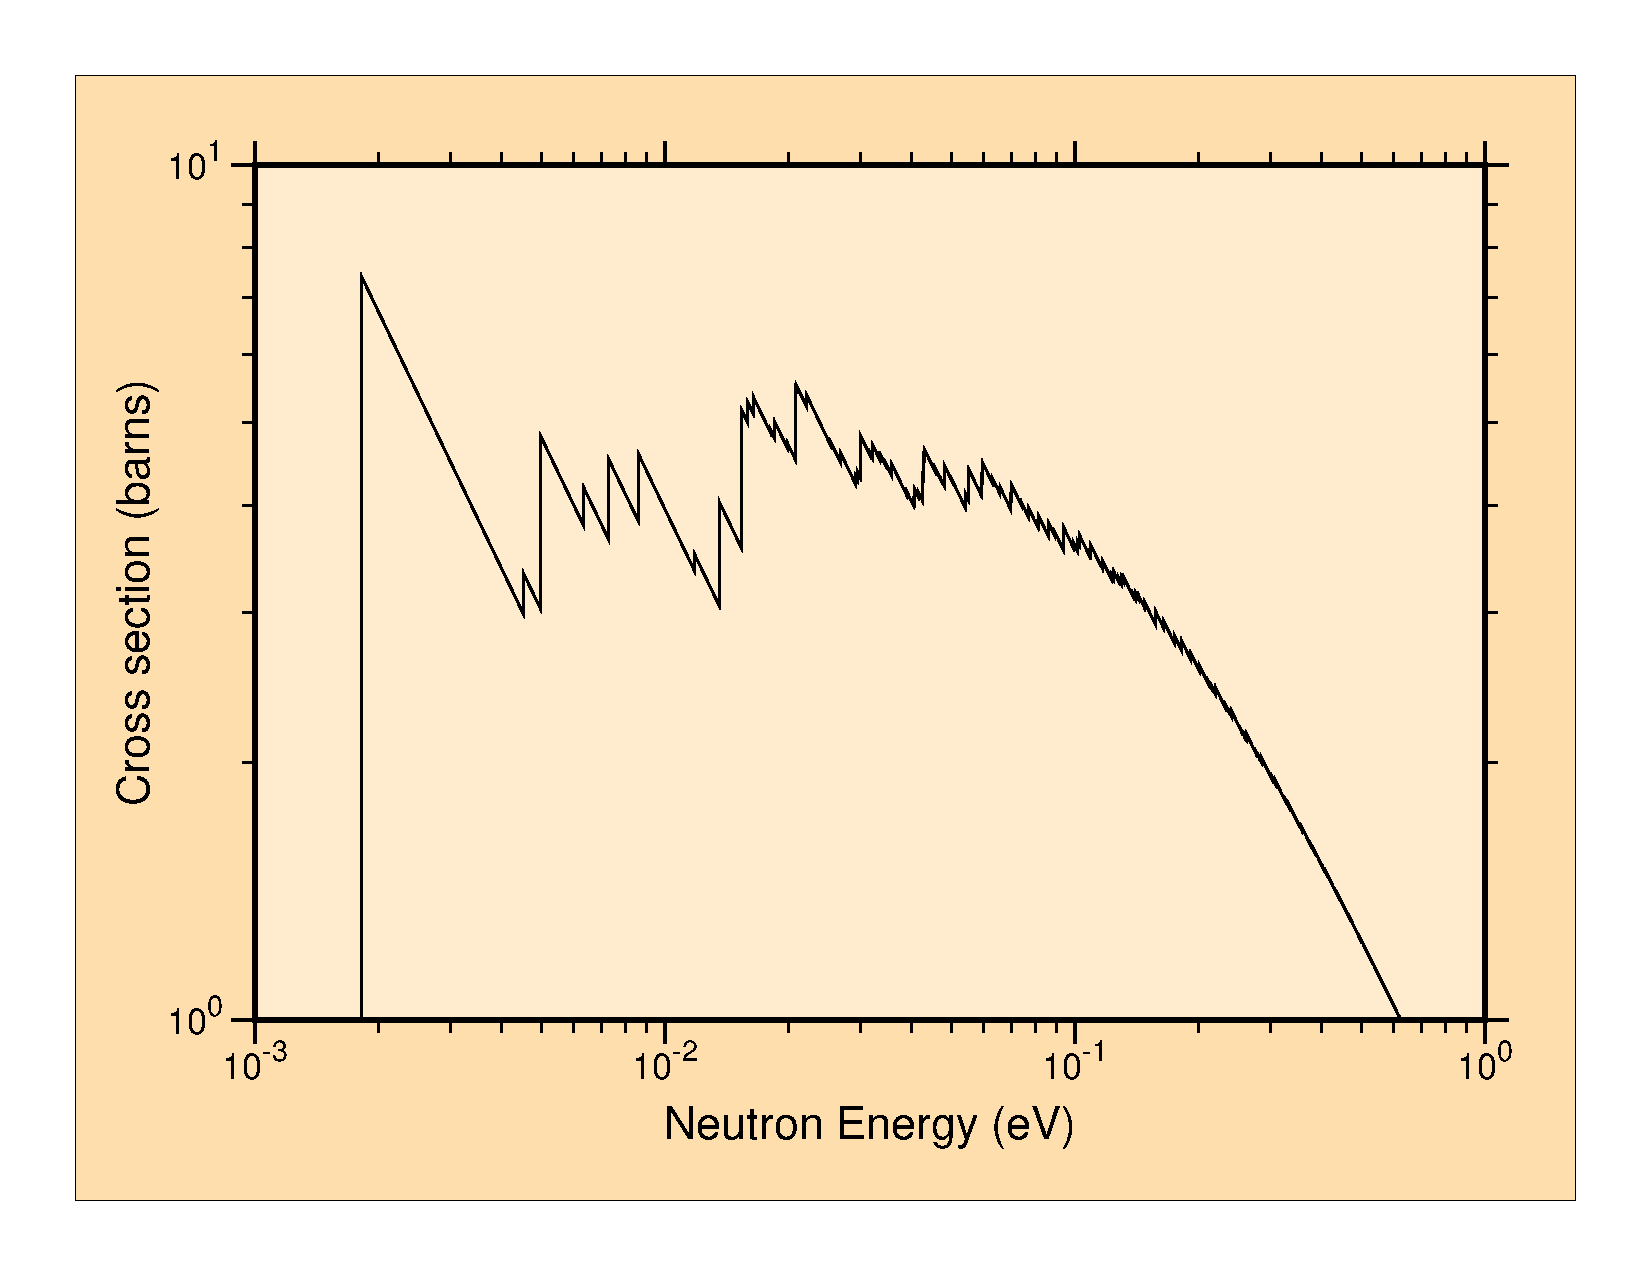
\includegraphics[keepaspectratio,height=3.5in, angle=0]{figs/thermr1ack}
\caption[Example of coherent elastic cross section for a crystalline
material (graphite)]
 {Typical behavior of the coherent elastic scattering cross section for a
 crystalline material as computed by THERMR. This cross section is for
 graphite at 293.6K.}
\label{cohfig}
\end{figure}

For evaluations in the ENDF-6 format, the section MF=7/MT=2 contains
the quantity $E\sigma^{\rm coh}(E)$ as a function of energy and
temperature. The energy dependence is given as a histogram with breaks
at the Bragg energies.  The cross section is easily recovered from this
representation by dividing by $E$.  The $E_i$ are easily found as the
tabulation points of the function, and the $f_i$ for a point can be
obtained by subtracting the value at the previous point.

For evaluations using the older ENDF/B-III thermal format, it is
necessary to compute the $E_i$ and $f_i$ in THERMR.  The methods used
are based on HEXSCAT\index{HEXSCAT} and work only for the hexagonal
materials graphite, Be, and BeO.  The Bragg edges are given by

\begin{equation}
   E_i=\frac{\hbar^2\tau_i^2}{8m}\,\,,
\end{equation}

\noindent
where $\tau_i$ is the length of the vectors of one particular
``shell'' of the reciprocal lattice, and $m$ is the neutron mass.
The $f_i$ factors are given by

\begin{equation}
   f_i=\frac{\pi^2\hbar^2}{2mNV}\sum_{\rm shell}|F(\tau)|^2\,\,,
\end{equation}

\noindent
where the shell sum extends over all reciprocal lattice vectors
of the given length, $N$ is the number of atoms in the unit cell,
and  $F$ is the crystallographic structure factor.  The calculation
works by preparing a sorted list of precomputed $\tau_i$ and $f_i$
values.  As $\tau_i$ gets large, the values of $\tau_i$ get more and more
closely spaced.  In order to save storage and run time, a range of $\tau$
values can be lumped together to give a single effective $\tau_i$ and
$f_i$.  This device washes out the Bragg edges at high energies while
preserving the proper average cross section and angular dependence.
The current grouping factor is 5\% (see \cword{eps} in \cword{sigcoh}).

Lattice constants (given in \cword{sigcoh} for graphite, Be, and BeO), form
factor formulas (see \cword{form}), Debye-Waller coefficients, and methods
for computing reciprocal lattice vectors were borrowed directly
 from HEXSCAT.

The energy grid for $E$ is obtained adaptively (see \cword{coh}).  A panel
extending from just above one Bragg edge to just below the next
higher edge is subdivided by successive halving until linear
interpolation is within a specified fractional tolerance (\cword{tol}) of the
exact cross section at every point.  This procedure is repeated for
every panel from the first Bragg edge to the specified maximum
energy for the thermal treatment (\cword{emax}).

The code usually computes and writes out the cross section of
Eq.~\ref{cohxs}, the average over $\mu$ of Eq.~\ref{coh},
which is sometimes called the P$_0$ cross section.  Subsequent modules can
deduce the correct discrete scattering angles $\mu_0$ from the
location of the Bragg edges $E_i$ and the factors $f_i$ from the
cross section steps at the Bragg edges (see
\hyperlink{sGROUPRhy}{GROUPR}\index{GROUPR}).
Legendre cross sections can also be computed by making a small change
to the code.  It is not necessary to give the P$_1$, P$_2$, and P$_3$ cross
sections explicitly as was done in some earlier codes or in File 4
of the ENDF thermal tapes.

\subsection{Incoherent Inelastic Scattering}
\label{ssTHERMR_incoh_inel}

In ENDF/B notation, the thermal incoherent scattering cross section
\index{incoherent inelastic} is given by

\begin{equation}
   \sigma^{\rm inc}(E,E',\mu)=\frac{\sigma_b}{2kT}
    \sqrt{\frac{E'}{E}}\,{\rm e}^{-\beta/2}S(\alpha,\beta)\,\,,
\label{incoh}
\end{equation}

\noindent
where $E$ is the initial neutron energy, $E'$ is the energy of the
scattered neutron, $\mu$ is the scattering cosine in the laboratory
system, $\sigma_b$ is the characteristic bound incoherent cross
section for the nuclide, $T$ is the Kelvin temperature, $\beta$ is the
dimensionless energy transfer,

\begin{equation}
   \beta=\frac{E'-E}{kT}\,\,,
\label{ebeta}
\end{equation}

\noindent
$\alpha$ is the dimensionless momentum transfer,

\begin{equation}
   \alpha=\frac{E'+E-2\mu\sqrt{EE'}}{AkT}\,\,,
\end{equation}

\noindent
$k$ is Boltzmann's constant\index{Boltzmann constant}, and $A$
is the ratio of the scatter mass to the neutron mass.  The
bound scattering cross section\index{bound atom scattering cross section}
is usually given in terms of the characteristic free cross
section,\index{free atom scattering cross section} $\sigma_f$,

\begin{equation}
   \sigma_b=\sigma_f\frac{(A+1)^2}{A^2}\,\,.
\end{equation}

\noindent
The scattering law\index{scattering law}
$S(\alpha,\beta)$\index{$S(\alpha,\beta)$} describes the binding of the
scattering atom in a material.  For a free gas\index{free gas}
of scatterers with no internal structure

\begin{equation}
   S(\alpha,\beta)=\frac{1}{\sqrt{4\pi\alpha}}
    \exp\left\{-\frac{\alpha^2+\beta^2}{4\alpha}\right\}\,\,.
\label{free}
\end{equation}

\noindent
For binding in solids and liquids, $S(\alpha,\beta)$ for a number of
important moderator materials is available in ENDF/B File 7
\index{File 7} format.  The scattering law is given as tables of $S$
versus $\alpha$ for various values of $\beta$.  Values of
$S$ for other values of $\alpha$ and $\beta$ can be obtained by interpolation.
The scattering law is normally symmetric in $\beta$ and only has to be
tabulated for positive values, but for materials like orthohydrogen and
parahydrogen\index{ortho hydrogen}\index{para hydrogen}
of interest for cold moderators at neutron scattering facilities,
this is not true.  These kinds of materials are identified by the ENDF-6 LASYM
option, and THERMR assumes that the scattering law is given explicitly
for both positive and negative values of $\beta$.

If the $\alpha$ or $\beta$ required is outside the range of the table
in File 7, the differential scattering cross section can be computed
using the short collision time (SCT) approximation
\index{short collision time}

\begin{equation}
   \sigma^{\rm SCT}(E,E',\mu)=\frac{\sigma_b}{2kT}
     \frac{\sqrt{E'/E}}{\sqrt{4\pi\,\alpha\,T_{\rm eff}/T}}
      \exp\left\{-\frac{(\alpha-|\beta|)^2}{4\,\alpha}
        \frac{T}{T_{\rm eff}}-\frac{\beta+|\beta|}{2}\right\}\,\,,
\end{equation}

\noindent
where $T_{\rm eff}$ is the effective temperature for the SCT approximation.
These temperatures are available\cite{GAreport} for the older
ENDF/B-III evaluations; they are usually somewhat larger
than the corresponding Maxwellian temperature $T$.  For the convenience
of the user, the values of $T_{\rm eff}$ for the common moderators are
included as defaults (see input instructions).  For the newer ENDF-6
format, the effective temperatures are included in the data file.
However, there is a complication.  Some evaluations give $S(\alpha,\beta)$ for
a molecule or compound (in the ENDF/B-III files, these cases are
BeO and C$_6$H$_6$).  The corresponding SCT approximation must contain
terms for both atoms.  The two sets of bound cross sections and effective
temperatures are included in the data statements in THERMR, and they
can be given in the new ENDF-6 format if desired.

THERMR expects the requested temperature $T$ to be one of the temperatures
included on the ENDF/B thermal file, or within a few degrees of that
value (296K is used if 300K is requested).  Intermediate temperatures
should be obtained by interpolating between the resulting cross sections
and not by interpolating $S(\alpha,\beta)$.

The cross sections for incoherent inelastic scattering are computed
in the \cword{calcem}\index{calcem@{\ty calcem}} subroutine.  There
are two possible orderings of the basic variables allowed (see
\cword{iform}).  For $E$-$E'$-$\mu$ ordering, the secondary energy grid
for incoherent scattering is obtained adaptively.  A stack is first primed
with the point at zero and the first point above zero that can be derived
from the positive and negative values of $\beta$ from the evaluator's
$\beta$ grid using Eq.~\ref{ebeta}.  (For free-gas scattering, the
$\beta$ grid is taken to have 30 entries between 0.0 and 400).
This interval is then subdivided by successive halving until the
cross section obtained by linear interpolation is within the specified
tolerance of the correct cross section (from
\cword{sigl}\index{sigl@{\ty sigl}}). The next
highest energy derived from the $\beta$ grid is then calculated,
and the subdivision process is repeated for this new interval.
This process is continued until the $\beta$ grid has been exhausted.
Excess points with zero cross section are removed before writing
the spectrum into File 6.  This procedure is sure to pick up all the
structure in the evaluation; giving points related to the $\beta$
grid avoids excessive work in trying to fit sharp corners introduced by
breaks in the interpolation of $S(\alpha,\beta)$.  Fig.~\ref{graph}
shows how the procedure picks up features resulting from the sharp
excitation features in the graphite phonon frequency distribution.

\begin{figure}[thb]\centering
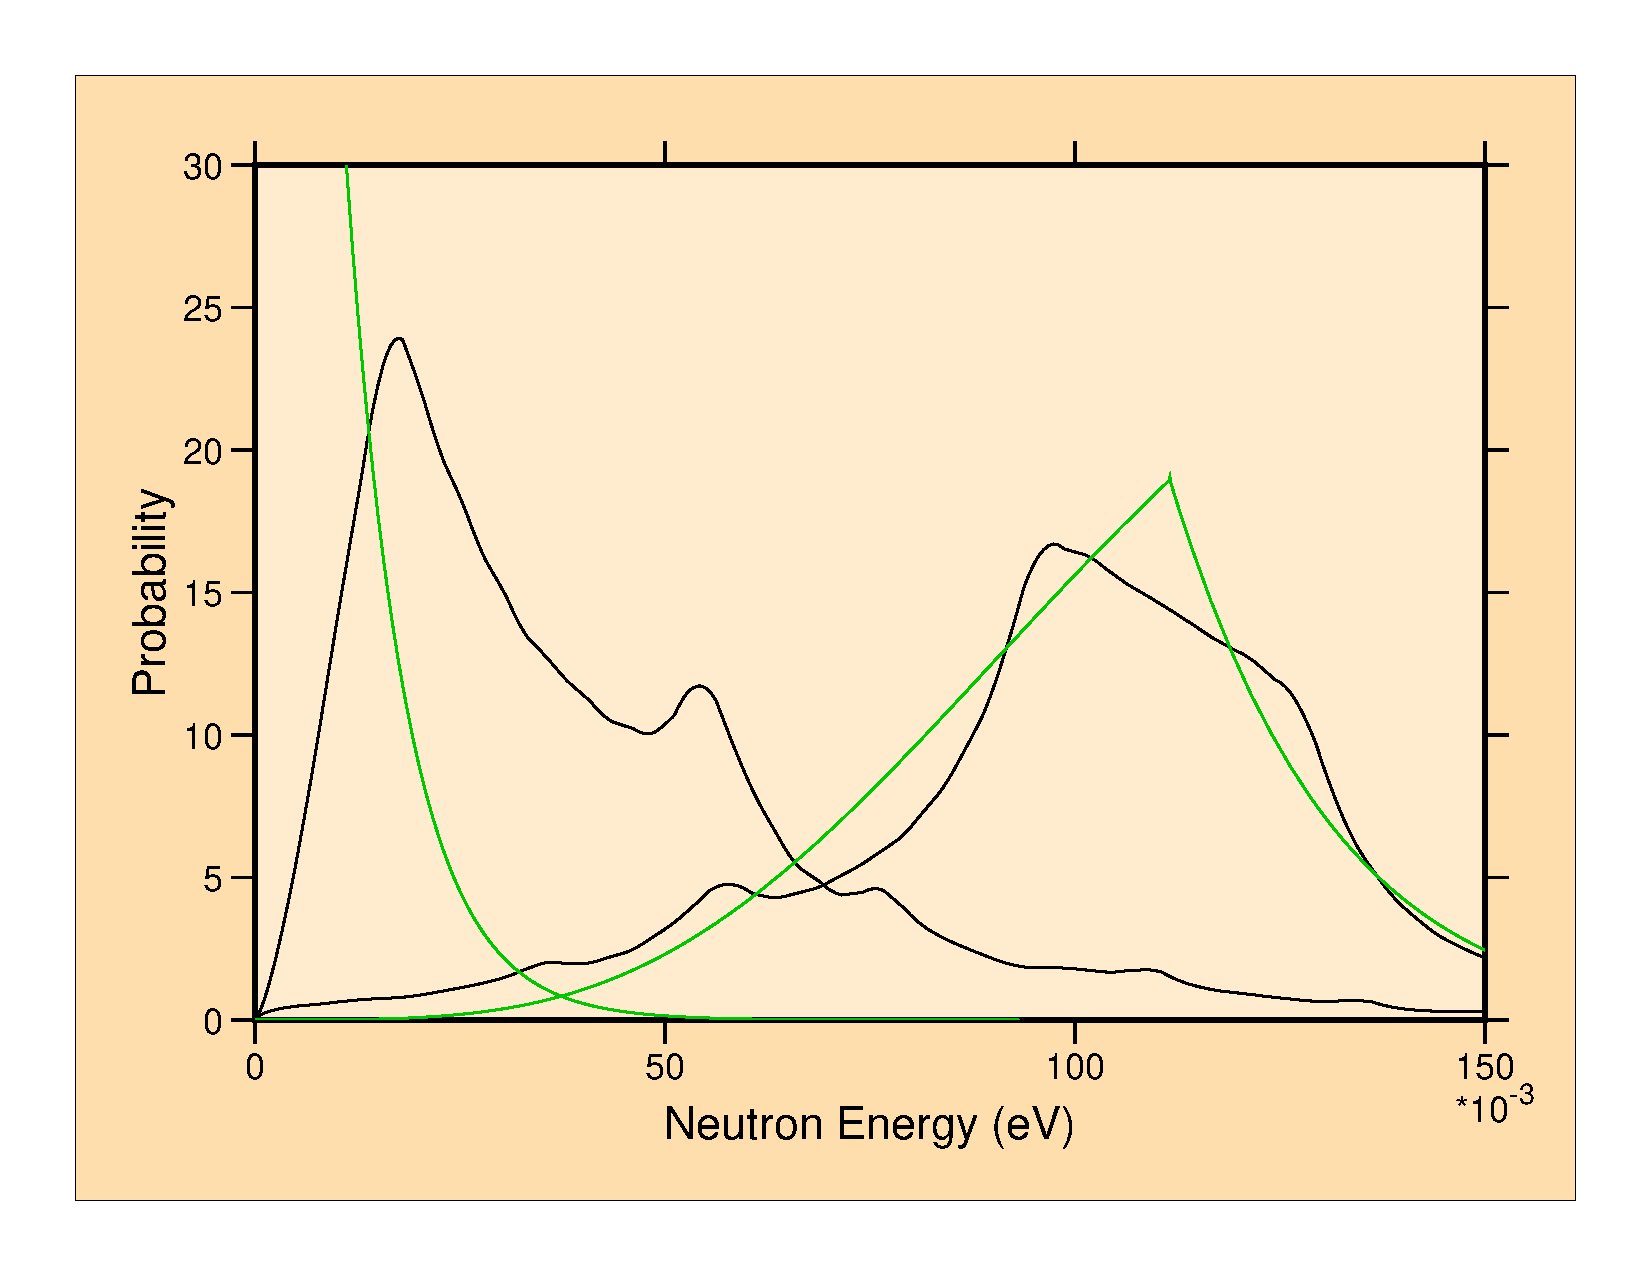
\includegraphics[keepaspectratio, height=3.0in, angle=0]{figs/thermr2ack}
  \caption[Adaptive reconstruction of emission spectra (graphite)]{Adaptive
 reconstruction of two of the emission curves for graphite at 293.6K
 (E=.00016 eV to the left, and E=.1116 eV to the right).  Note the
 presence of excitation features from the phonon frequency spectrum
 for both upscatter and downscatter.  The breaks in the curves are due
 to $\beta$ interpolation in $S(\alpha,\beta)$ and not to the tolerances
 in the reconstruction process.  The green curves are the corresponding
 free gas results.}
\label{graph}
\end{figure}

The result of this adaptive reconstruction is easily integrated by the
trapezoid rule to find the incoherent cross section at energy $E$.

The cross section for one particular $E{\rightarrow}E'$ is the integral
over the angular variable of Eq.~\ref{incoh}.  The angular dependence
is obtained by adaptively subdividing the cosine range until the actual
angular function (see \cword{sig}\index{sig@{\ty sig}}) is represented
by linear interpolation to within a specified tolerance.  The integral
under this curve is used in calculating the secondary-energy dependence
as described above.  Rather than providing the traditional Legendre
coefficients, THERMR divides the angular range into equally probable
cosine bins and then selects the single cosine in each bin that
preserves the average cosine in the bin.  These equally probable
cosines can be converted to Legendre coefficients easily
when producing group constants, and they are suitable for direct use in
Monte Carlo codes.  For strongly peaked functions, such as scattering for
$E{\gg}kT$ when the result begins to look ``elastic'', all the discrete
angles will be bunched together near the scattering angle defined by
ordinary kinematics.  This behavior cannot be obtained with ordinary
P$_3$ Legendre coefficients.  Conversely, if such angles are converted to
Legendre form, very high orders can be used.  If a direct calculation of
Legendre components is desired, reverse the sign of \cword{nnl} in
\cword{calcem}.

The incident energy grid\index{thermal energy grid} is currently stored
directly in the code (see \cword{egrid} in \cword{calcem}).  The choice
of grid for $\sigma^{\rm inc}(E)$ is not critical since the cross section
is a slowly varying function of $E$.  However, the energy grid
would seem to be important for the emission spectra.  In order
to demonstrate the problem, two perspective plots of
the full energy distribution of incoherent inelastic scattering from
graphite at 293.6K are shown in Figs.~\ref{dist} and \ref{dist2}.
The second plot is simply an expansion of the high-energy region
of the distribution.

\begin{figure}[thb]\centering
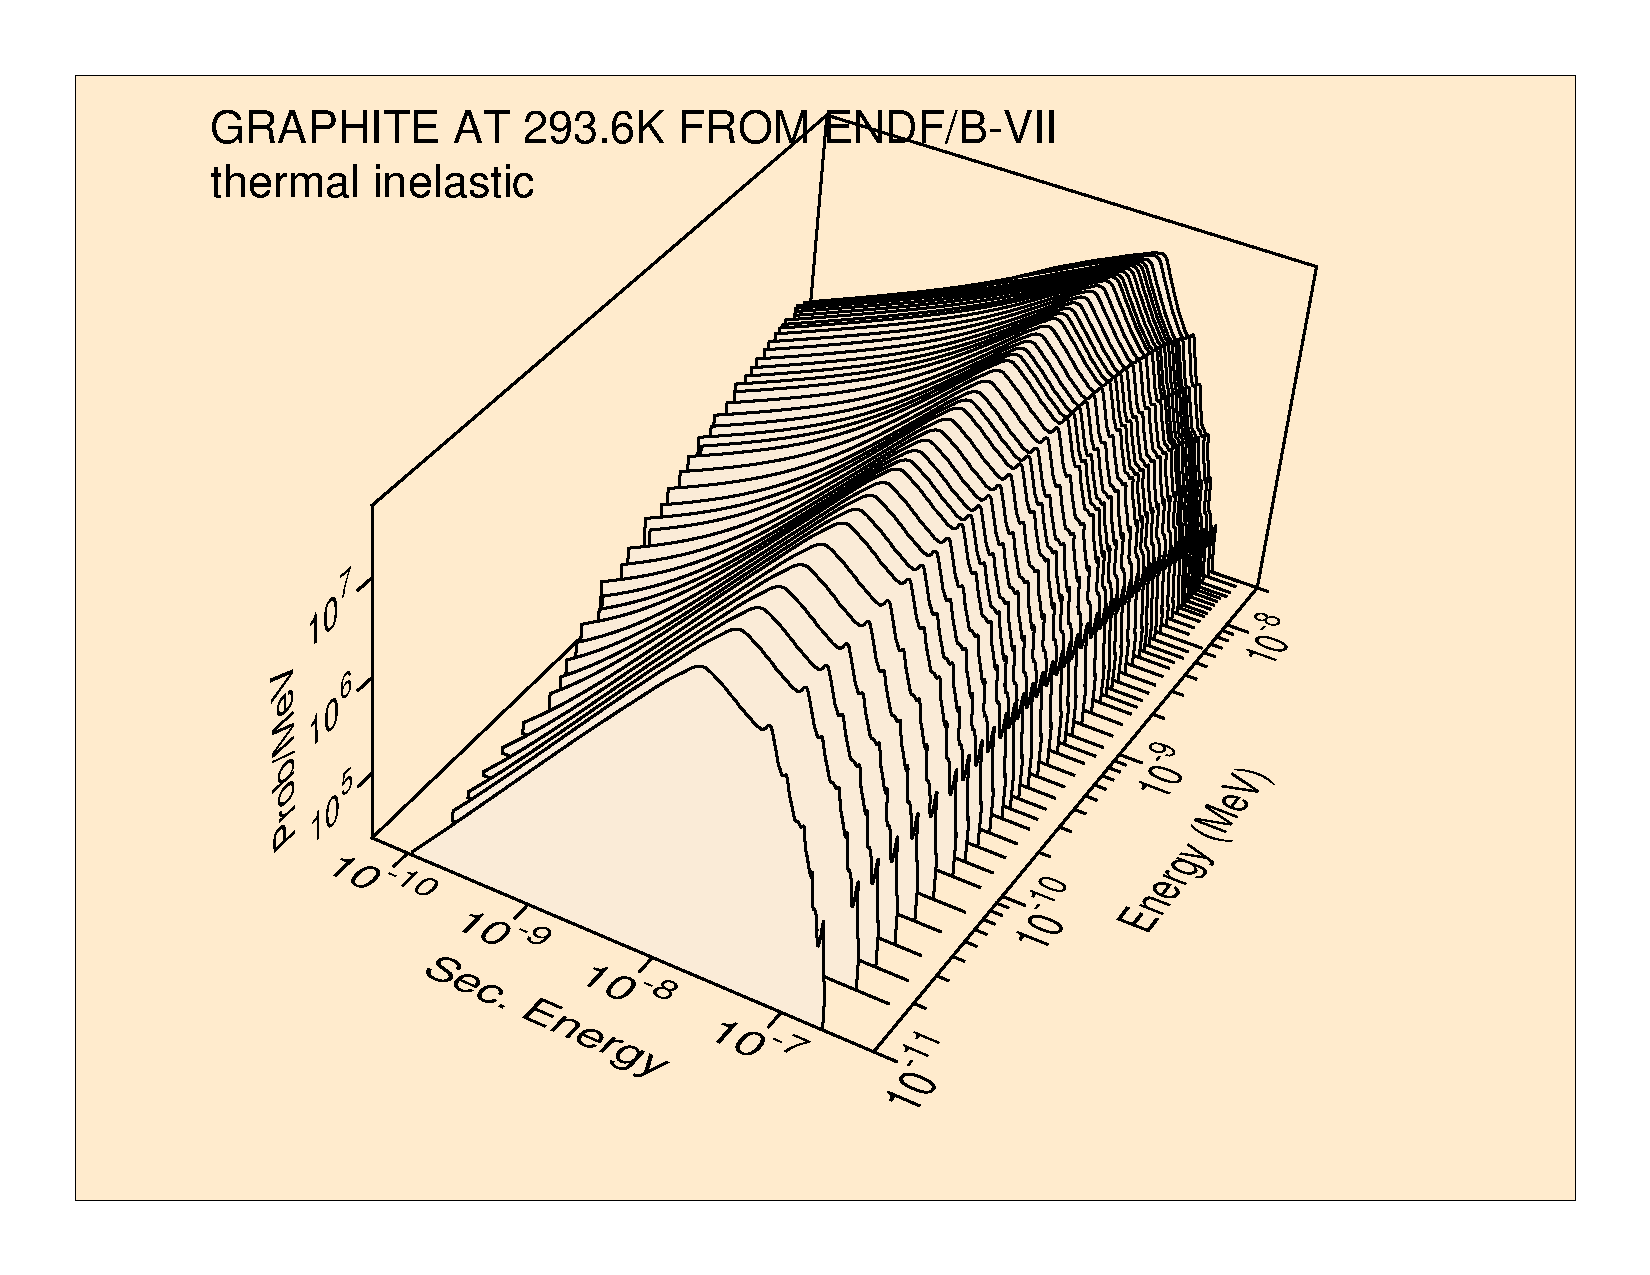
\includegraphics[keepaspectratio,height=3.0in, angle=0]{figs/thermr3ack}
\caption[Neutron distribution for incoherent inelastic scattering from graphite
 (T = 293.6K)]{Neutron distribution for incoherent inelastic scattering from
 graphite (T = 293.6K).}
\label{dist}
\end{figure}

\begin{figure}[thb]\centering
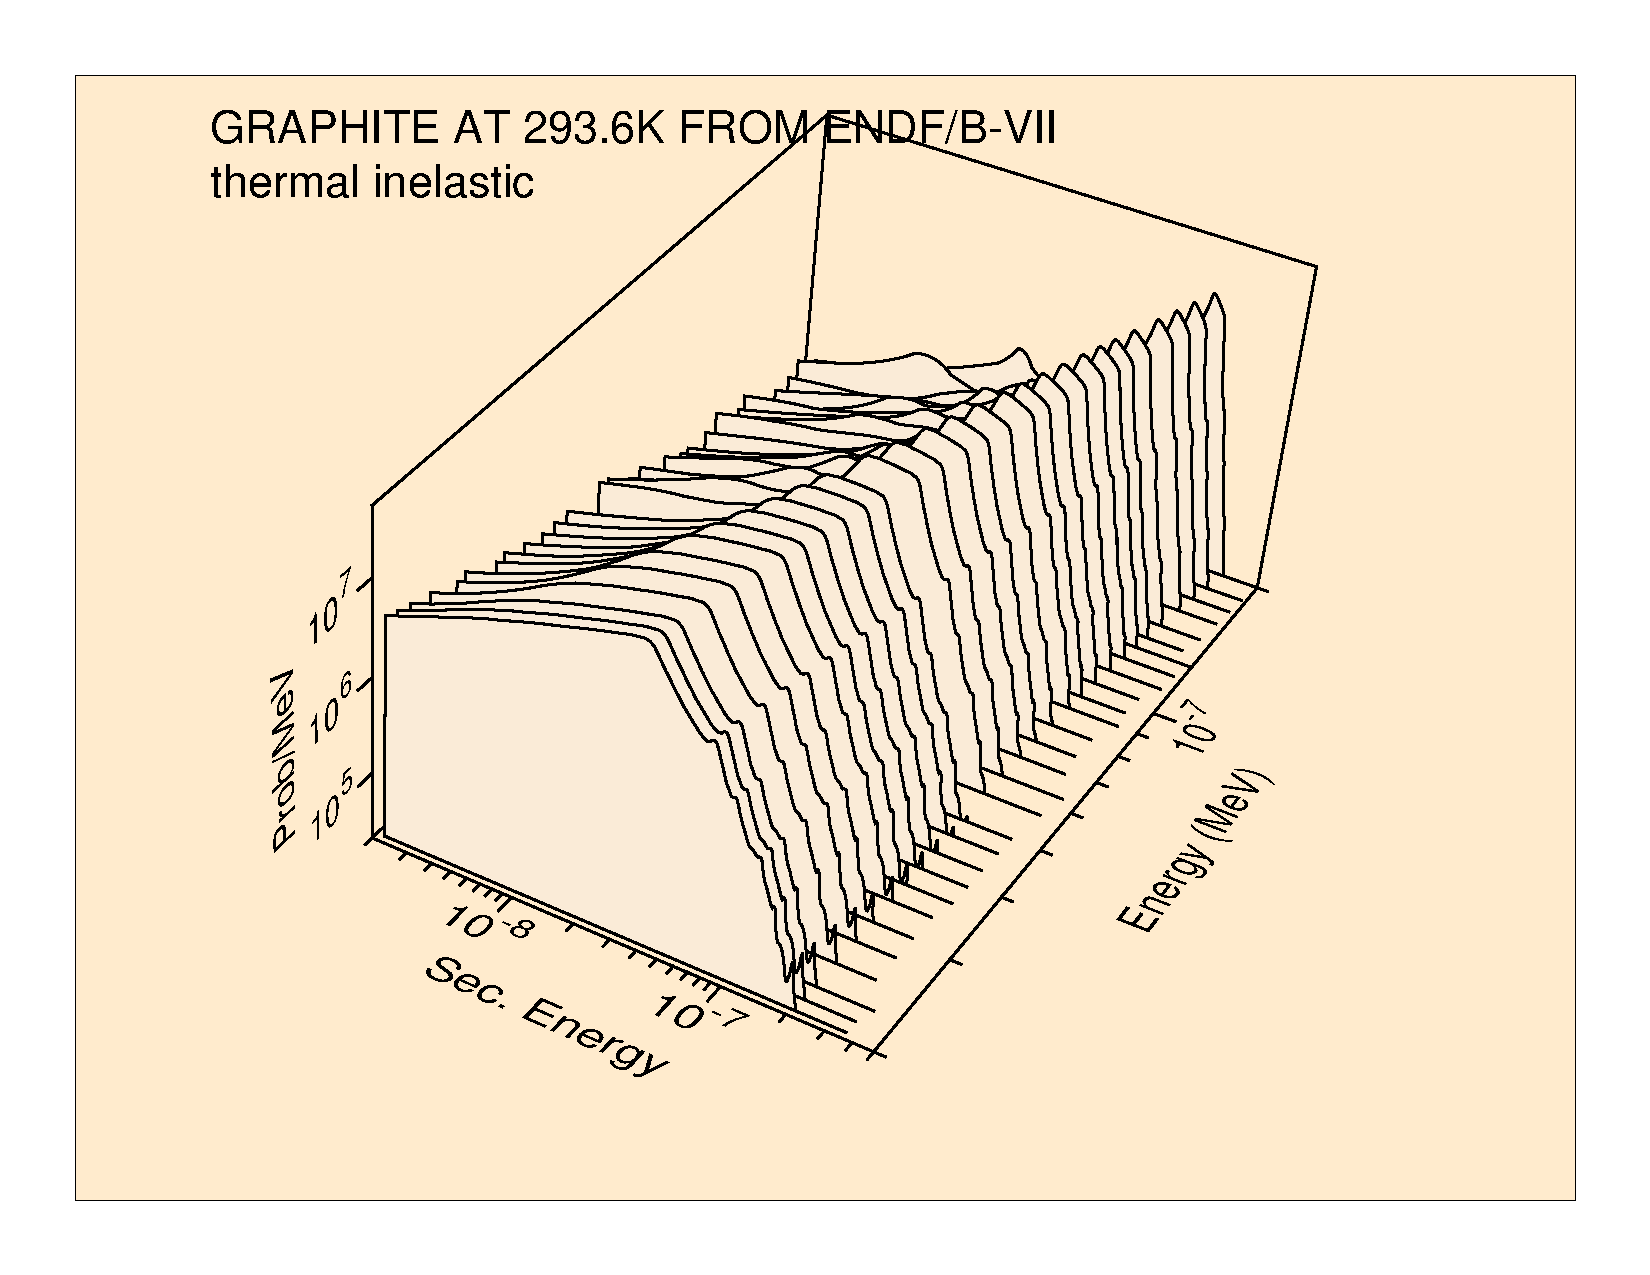
\includegraphics[keepaspectratio, height=3.0in, angle=0]{figs/thermr4ack}
  \caption[Neutron distribution for incoherent inelastic scattering
  from graphite
 (T = 293.6K), expanded view]{Expanded view of the high-energy region
 of the graphite incoherent inelastic distribution.}
\label{dist2}
\end{figure}

It is clear that $\sigma^{\rm inc}(E,E')$ for one value of $E'$ is
a very strongly energy-dependent function for the higher incident
energies.  However, as shown in Fig.~\ref{dist2}, the shape
of the secondary energy distribution changes more slowly,
with the peak tending to follow the line $E'{=}E$.  This behavior
implies that a relatively coarse incident energy grid might prove
adequate if a suitable method is used to interpolate between the
shapes at adjacent $E$ values.  One such interpolation scheme is
implemented in \hyperlink{sGROUPRhy}{GROUPR}\index{GROUPR}.  The
use of discrete angles is
especially suitable for this interpolation scheme.

Strictly speaking, the scattering law for free-gas scattering
given in Eq.~\ref{free} is only applicable to scatterers with no
internal structure.  However, many materials of interest in reactor
physics have strong scattering resonances in the thermal range
(for example, $^{240}$Pu and $^{135}$Xe).  The Doppler broadened elastic
cross section produced by BROADR\index{BROADR} is formally correct for
a gas of resonant scatterers, but the cross section resulting from
Eq.~\ref{free} is not.  In order to allow for  resonance scattering
in a way that at least provides the correct total cross section, THERMR
renormalizes the free-atom scattering to the broadened elastic cross
section.  The secondary energy distribution will still be incorrect.

The built-in grid for incident neutron energies is suitable for
normal temperatures found in reactors.  For higher temperatures
(higher than \cword{break}=3000), the grid values are scaled up
to span the kinds of energies expected.

If the $E$-$\mu$-$E'$ option is selected (\cword{iform}=1), an
adaptive reconstruction of the angular cross section
$\sigma(E,\mu)$ is performed.  For each $\mu$ value, the
secondary energy spectrum is generated adaptively, and the
integral over that spectrum is saved as $\sigma(E,\mu)$.
The results are written out using the ENDF-6 format
File 6/law 7 option.  This ordering is more like the results
of experiments, and the THERMR results can be used to compare
to experiment.  See Fig.~\ref{ang2} for a figure based on
this kind of ordering.

\begin{figure}[thb]\centering
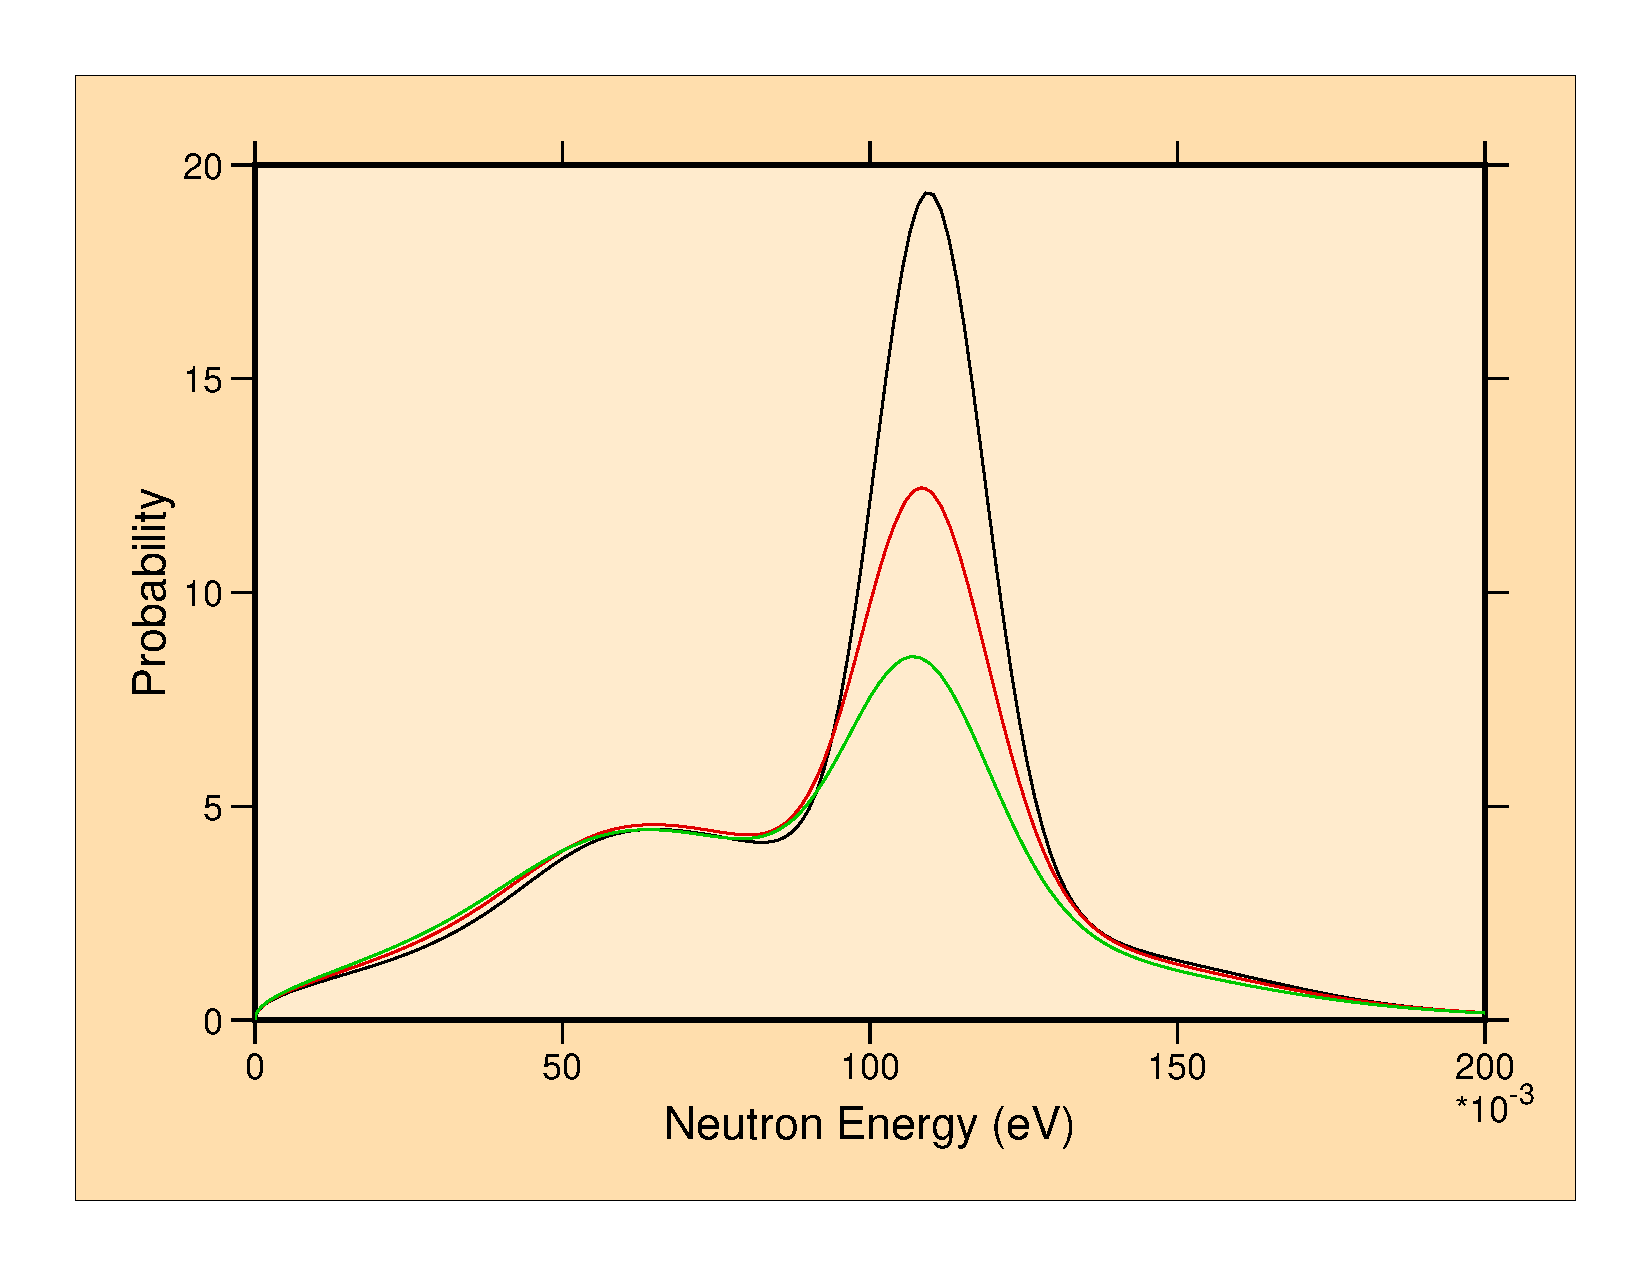
\includegraphics[keepaspectratio, height=3.5in, angle=0]{figs/thermr7ack}
\caption[Distributions for H in H$_2$O with $E$-$\mu$-$E'$ ordering]
{Example of distributions for H in H$_2$O with $E$-$\mu$-$E'$ ordering.  The
 incident energy is 0.115 eV.  The black curve is at 51.3 deg, the red
 curve is at 60 deg, and the green curve is at 68 deg.}
\label{ang2}
\end{figure}

\subsection{Incoherent Elastic Scattering}
\label{ssTHERMR_incoh_el}

In hydrogenous solids, there is an elastic (no energy loss) component
of scattering arising from the zero-phonon term that can be treated in
the incoherent approximation because of the large incoherent cross
section of hydrogen.  The ENDF term for this process is incoherent
elastic scattering\index{incoherent elastic}, and it is found in the
materials polyethylene and zirconium hydride.
\index{polyethylene}
\index{zirconium hydride}
The differential cross section is given by

\begin{equation}
   \sigma^{\rm iel}(E,E',\mu)=\frac{\sigma_b}{2}
     {\rm e}^{-2WE(1-\mu)}\,\delta(E-E')\,\,,
\end{equation}

\noindent
where $\sigma_b$ is the characteristic bound cross section and $W$ is the
Debye-Waller coefficient\index{Debye-Waller factor}.  The energy grid
of the elastic cross section is used for $E$, and the average cross
section and equally probable angles are computed using

\begin{equation}
   \sigma^{\rm iel}(E)=\frac{\sigma_b}{2}\left\{
     \frac{1-{\rm e}^{-4WE}}{2WE}\right\}\,\,,
\end{equation}

\noindent
and

\begin{eqnarray}
   \bar{\mu}_i&=&\frac{N}{2WE}\left[
      {\rm e}^{-2WE(1-\mu_i)}(2WE\mu_i-1)\right.\nonumber\\
      &-&\left.{\rm e}^{-2WE(1-\mu_{i-1})}(2WE\mu_{i-1}-1)
      \right]/(1-{\rm e}^{-4WE})\,\,,
\end{eqnarray}

\noindent
where

\begin{equation}
   \mu_i=1+\frac{1}{2WE}\ln\left[
       \frac{1-{\rm e}^{-4WE}}{N}+{\rm e}^{-2WE(1-\mu_{i-1})}
        \right]
\end{equation}

\noindent
is the upper limit of one equal probability bin and $\bar{\mu}_i$ is
the selected discrete cosine in this bin.  Here $N$ is the number of bins
and $\mu_0$ is $-1$.

The characteristic bound cross sections and the Debye-Waller coefficients
can be read from MF=7/MT=2 of an ENDF-6 format evaluation, or obtained
directly from data statements in the code for the older format.

\subsection{Coding Details}
\label{ssTHERMR_details}

The \cword{thermr}\index{thermr@{\ty thermr}} routine comes from
module \cword{thrmm}\index{modules!thrmm@{\ty thrmm}}.  The
procedure begins with the reading of the user's input.
The required ENDF tape (\cword{nendf}) is only used for MF=7 data;
it can be set to zero if only free-gas scattering is needed.  Similarly,
\cword{matde} is the material number for the File 7 tape and can be
set to zero for free-atom problems.  The ENDF File 7 format only
gives ``M$_0\,\sigma_{f0}$'', the product of the free scattering cross
section for the principal scatterer and the number of principal scatterer
atoms in the molecule.  As a result, THERMR needs the parameter
\cword{natom} to obtain the effective microscopic cross section
(for example, for H in H$_2$O, use \cword{natom}=2).  For ENDF/B-III
format files, default parameters are supplied for mixed moderators
(BeO and benzine) and effective temperatures, if needed.

Continuing, \cword{thermr} finds the desired material on the input
PENDF\index{PENDF} and ENDF tapes.  It will automatically loop over
\cword{ntemp} materials on \cword{nin}.  The input tape must have been
through \hyperlink{sBROADRhy}{BROADR}\index{BROADR}.  The
elastic cross section at the current
temperature is saved on a \cword{loada/finda} scratch file to be used
for normalizing free-atom scattering if necessary.  For ENDF-6 format
materials, the parameters for the elastic calculation are read in
using \cword{rdelas}\index{rdelas@{\ty rdelas}}.  Next,
\cword{thermr} computes elastic and/or inelastic cross sections by
calls to \cword{coh}\index{coh@{\ty coh}},
\cword{iel}\index{iel@{\ty iel}}, and
\cword{calcem}\index{calcem@{\ty calcem}}.  Finally,
the results are written onto the output PENDF tape by
\cword{tpend}\index{tpend@{\ty tpend}}.

Some alteration of ENDF/B formats and conventions was required to
accommodate thermal cross sections.  The incoherent inelastic cross
sections fit well into MF=3 using MT=\cword{mtref} (see user input).
The coherent or incoherent elastic cross section (if present) uses
\cword{mtref}+1.  Other modules of NJOY expect that thermal MT numbers
will be between 221 and 250.  The incoherent energy-to-energy matrix is
stored in MF=6 (coupled angle-energy distributions).  Before the
introduction of the ENDF-6 format, the ENDF File 6 formats were not
well-suited to this application because secondary angle and energy
were not tightly coupled as required by the physics of the problem.
Therefore, three new formats were defined for File 6:
LTT=5 for discrete-angle inelastic transfer cross sections,
LTT=6 for discrete-angle elastic data, and
LTT=7 for coherent elastic reactions.
The format for LTT=5 follows in the notation of ENDF-102\cite{old102}:

\small
\begin{ccode}

   MAT,6,MT [ ZA, AWR, 0, LTT, 0, 0 ] CONT  LTT=5
   MAT,6,MT [ T, 0., 0, 1, NNE / NNE, 2 ] TAB2
   MAT,6,MT [ 0., EN, 0, 0, NEP*(NL+1), NL+1 /
              EP(1), PP(1), EPM(1,1), ...
              EP(2), PP(2), ... ] LIST
      ... repeat the LIST for the NNE values of EN ...
   MAT,6,0  [ 0., 0., 0, 0, 0, 0 ] SEND

\end{ccode}
\normalsize

\noindent
There is a list record for each of the NNE values of incident
energy.  Each list record gives the normalized secondary energy
distribution as NEP values of PP vs. $E'$, and for each value of $E'$,
the record gives NL equally probable cosines, EPM.
Similarly, the format for LTT=6 is:

\small
\begin{ccode}

   MAT,6,MT [ ZA, AWR, 0, LTT, 0, 0 ] CONT  LTT=6
   MAT,6,MT [ T, 0., 0, 1, NNE / NNE, 2 ] TAB2
   MAT,6,MT [ 0., EN, 0, 0, NU+2, NU+2 /
              EN, 1., U(1), U(2), ... ] LIST
      ... repeat the LIST for the NNE values of EN ...
   MAT,6,0  [ 0., 0., 0, 0, 0, 0 ] SEND

\end{ccode}
\normalsize

\noindent
Here, there is just a set of NU equally probable cosines given
for each incident energy.  Note that this format was designed to
look like that for LTT=5 with NEP=1.
Finally, the format for LTT=7 is:

\small
\begin{ccode}

   MAT,6,MT [ ZA, AWR, 0, LTT, 0, 0 ] CONT  LTT=7
   MAT,6,MT [ 0,, 0., 0, 0, 0, NBRAGG ] CONT
   MAT,6,0  [ 0., 0., 0, 0, 0, 0 ] SEND

\end{ccode}
\normalsize

\noindent
In this case, all the important information is in File 3 under
MT=\cword{mtref}+1.  For convenience, the number of Bragg edges
used is given here in File 6 as NBRAGG.

In subroutine \cword{coh}\index{coh@{\ty coh}}, the energy grid
is determined adaptively and stored into the same \cword{loada/finda}
\index{loada/finda@{\ty loada/finda}} scratch file used for
the elastic cross section.  The elastic cross section is converted to
the coherent grid using Lagrangian interpolation (see \cword{terp}).
\index{terp@{\ty terp}} The structure of the record stored on the
scratch file is [energy / static elastic / incoherent inelastic
/ coherent elastic].

Coherent cross sections at a given energy $E$ are computed by
\cword{sigcoh}\index{sigcoh@{\ty sigcoh}}.  If this is the first
entry ($E{=}0$) for an ENDF-III type material, the appropriate
lattice constants are selected and the Debye-Waller coefficient
is obtained for the desired temperature by interpolation.  Then
the reciprocal lattice wave vectors and structure factors are
computed, sorted into shells, and stored for later use.  On
a normal entry ($E{>}0$), the stored list is used to
compute the cross section.  For ENDF-6 format materials, the
initialization step is used to organize the data already read
from MF=7/MT=2 by \cword{rdelas}, and subsequent entries are used
to compute the cross section.

Incoherent elastic cross sections are computed in subroutine
\cword{iel}\index{iel@{\ty iel}}.  The appropriate bound cross sections
and Debye-Waller coefficients are either extracted from the data already
read from an ENDF-6 format MF=7/MT=2 by \cword{rdelas}, or they are
extracted from data statements in \cword{iel}\index{iel@{\ty iel}}
and then adjusted to the specified temperature using
\cword{terp}\index{terp@{\ty terp}} or \cword{terpa}\index{terpa@{\ty terpa}}.
The angle-integrated cross section is computed analytically on the grid
of the static elastic cross section and written back onto the
\cword{loada/finda} scratch file in the same slot used for coherent
elastic as described above (both never occur simultaneously in the
same material).  The discrete equally probable cosines are cast
into LTT=7 format and written onto a scratch tape for use by
\cword{tpend}\index{tpend@{\ty tpend}}.

Incoherent cross sections and distributions are generated in
\cword{calcem}\index{calcem@{\ty calcem}}.  On the first entry,
the ENDF/B scattering law is read in or parameters are set for
free-atom scattering.  For ENDF-6 files, the effective temperatures
for the SCT approximation are read in.  For the older formats, these
numbers were either read in or set to default values during the user
input process.  The calculation for $E$-$E'$-$\mu$ ordering (\cword{iform}=0)
goes through statement 300. An adaptive loop to determine the
secondary energy grid is carried out.  The required cross sections and
discrete cosines are returned by \cword{sigl}\index{sigl@{\ty sigl}},
which uses \cword{sig}\index{sig@{\ty sig}} to compute the
differential cross sections.  Because the spectrum curve will
have discontinuities in slope at energies corresponding to the break points
of the $\beta$ grid, it is important to use these energies as the starting
points for the adaptive reconstruction.  The first panel starts at $E'=0$
and ends at the first energy greater than zero that can be derived from
the $\beta$ grid.  This will normally be a negative $\beta$ value
corresponding to $E'{<}E$.  These two energies and their corresponding
cross sections are loaded into an inverted stack like the one used in
\hyperlink{sRECONRhy}{RECONR}.  Next, the top interval in the
stack is divided in half, and new
cross sections are computed at this midpoint.  If the new cross section
is not within the desired tolerance of the value obtained by linear
interpolation between the adjacent points, the new value is inserted into
the stack.  Otherwise, the top value in the stack is converged and can be
saved to the location where the spectrum is accumulating.  Each time the
stack gets down to a single element, a new point is calculated from the
next $\beta$ value in the evaluator's $\beta$ grid, and the subdivision
process is continued.  During this reconstruction process, the integrated
cross section is computed by adding in each trapezoid.  In addition, note
is taken of the last nonzero cross section value in order to remove excess
zero values from the end of the record.  The $\sigma$ vs. $E'$ curve is
complete when the $\beta$ grid has been exhausted (the highest positive
value).  The result is put directly into the modified MF=6 format and
written onto a scratch file.

When all the desired incident energies have been processed, the incoherent
cross section is calculated on the File 3 energy grid by interpolating
in the table of values computed by the reconstruction process.  The
results are stored on the \cword{loada/finda} tape.  If free-atom
scattering has been selected, the elastic cross section is stored in
the incoherent slot.

Incoherent inelastic scattering cross sections and discrete cosines are
computed in \cword{sigl}\index{sigl@{\ty sigl}}.  The stack for
the adaptive reconstruction of the angular distribution for a
given $E{\rightarrow}E'$ is primed with $\mu{=}{-}1$,
$\mu{=}{+}1$, and the angle for static scattering.  The top
interval on the stack is subdivided by halving until the actual cross
section computed by \cword{sig} is within a specified tolerance of a linear
interpolate.  As each panel is converged, its area is added to the
accumulating cross section.  On convergence, the fraction of the cross
section corresponding to each equally probable bin is computed, and
the linearization process is repeated to find the bin boundaries and
discrete cosines.  Note that Legendre coefficients can be computed in
this routine from the discrete cosines.

Subroutine \cword{sig}\index{sig@{\ty sig}}
is used to compute the actual double-differential
cross section for a given value of $E$, $E'$, and $\mu$.  This
is done using $S(\alpha,\beta)$ (with the possible use of the SCT
approximation for large values of $\alpha$ or $\beta$), or using
the free-gas scattering law.   Normally, $s(\alpha,\beta)$ is
symmetrical in $\beta$ and results are extracted from the table at
\cword{isab} using $|\beta|$.  However, this is not true for materials
like orthohydrogen and parahydrogen.  In these cases, the LASYM
parameter is set, and explicit $S(\alpha,\beta)$ values are given
for both negative and positive $\beta$.  For liquids, the presence
of diffusion leads to a singularity for $\beta=0$ and small $\alpha$
(the quasi-elastic scattering peak).  The normal ENDF interpolation
laws do not represent $S(\alpha,\beta)$ well in this region.  Therefore,
THERMR tries to determine if the material is a liquid by looking
at the small-$\alpha$ behavior of the $\beta=0$ curve (see \cword{cliq}).
It then extrapolates low-$\beta$ curves to low-$\alpha$ values
using a $\beta^2/\alpha$ law.

The calculation for $E$-$\mu$-$E'$ ordering starts at statement number 510.
In a loop over incident energies, subroutine
\cword{sigu}\index{sigu@{\ty sigu}} is called
to reconstruct $\sigma(E,\mu)$ adaptively.  The method used is
the same as that described above for the energy distribution, and
the result represents the angular cross section to within a desired
tolerance.  The inelastic cross section is obtained as the integral
over the angular cross section.  Subroutine \cword{sigu} obtains
the secondary energy spectrum corresponding to E and $\mu$
adaptively.  It uses the beta values from the evaluation as
starting points for subdivision, just as described above for
$E$-$E'$-$\mu$ ordering.  It uses \cword{sig}\index{sig@{\ty sig}}
to obtain the cross section for a given $E$, $E'$, and $\mu$.
The results of this calculation are written onto \cword{nscr} using
the ENDF-6 File 6/Law 7 format and passed to
\cword{tpend}\index{tpend@{\ty tpend}}.

Finally, \cword{tpend}\index{tpend@{\ty tpend}} is called to prepare
the output tape.  The File 1 directory is updated to account for
the new sections that are being added.  File 3 is located and
the cross sections stored on the \cword{loada/finda}
scratch file are retrieved, formatted, and written to the output tape.
Note that the elastic cross section in MT=2 and the total cross section in
MT=1 are not changed from their static values, nor is the union grid
updated.  As a result, MT=221 -- 250 must be considered supplemental.
Subsequent modules could ignore them or use them in place of the static
values.  Also note that it is possible to run THERMR several times with
different values of \cword{mtref}.  The result would be one PENDF tape
containing static cross sections and cross sections for several different
binding states that can be selected at will (for example, MT=2 for static
hydrogen, MT=221 for free hydrogen, MT=222 for hydrogen in water, and
MT=223 and MT=224 for hydrogen in polyethylene, all on one PENDF tape).

File 6 distributions are read from a scratch file (\cword{nscr})
in ENDF format, normalized, and written back onto the final tape.
Since free incoherent scattering was set equal to elastic scattering
in \cword{calcem}\index{calcem@{\ty calcem}}, the approximate
resonance correction of the matrix is now complete.

\subsection{Using the ENDF/B Thermal Data Files}
\label{ssTHERMR_ENDF}

The thermal data files originally prepared for
ENDF/B-III\index{ENDF!ENDF/B-III} were also
used for ENDF/B-IV and ENDF/B-V.\footnote{The data files and the
reference manual\cite{GAreport} are available from the National
Nuclear Data Center, Brookhaven National Laboratory, Upton, NY 11973.
Request Tapes 320 through 325 and report ENDF-269.}  Table~\ref{th1}
summarizes the contents of these data tapes.

\begin{table}[t]
\caption[ENDF/B-III Thermal Data Files]{Moderator Materials on
ENDF/B-III Thermal Data Tapes Showing Their MAT Numbers and
Distribution Tape Numbers}
\label{th1}
\begin{center}
%\small
\begin{tabular}{lcclcl}
   Material         &  MAT  &  Tape  &  MTs   & elastic & secondary \\
  \hline
   Be               &  1064  &  321  &  231,232  &  coh  &           \\
   BeO              &  1099  &  321  &  233,234  &  coh  &  none     \\
   C (graphite)      &  1065  &  322  &  229,230  &  coh  &           \\
   H(CH$_2$)  &  1114  &  322  &  223      &  iel  &  free C   \\
   C$_6$H$_6$       &  1095  &  325  &  227      &       &  none     \\
   D(D$_2$O)        &  1004  &  320  &  228      &       &  free O   \\
   H(H$_2$O)        &  1002  &  320  &  222      &       &  free O   \\
   Zr(ZrH$_n$)      &  1096  &  323  &  235,236  &  iel  &  1097     \\
   H(ZrH$_n$)       &  1097  &  323  &  225,226  &  iel  &  1096     \\
  \hline
\end{tabular}
\end{center}
\end{table}

\begin{table}[b]
\caption[ENDF/B-VII Thermal Data Files]{ENDF/B-VII Moderator Materials
with Their MAT and MT Numbers}
\label{th2}
\begin{center}
%\small
\begin{tabular}{lrlcl}
   Material         &  MAT  &  MTs   & elastic & secondary \\ \hline
   Al               &  45   &  243,244  &  coh  &          \\
   Be               &  26   &  231,232  &  coh  &          \\
   Be(BeO)          &  27   &  233,234  &  coh  &          \\
   O(BeO)           &  28   &  237,238  &  coh  &          \\
   C(graphite)      &  31   &  229,230  &  coh  &          \\
   Fe               &  56   &  245,246  &  coh  &          \\
   H(CH$_2$)           &  37   &  223      &  iel  & free C   \\
   H(liquidCH$_4$)     &  33   &           &       &          \\
   H(solidCH$_4$)      &  34   &           &       &          \\
   C$_6$H$_6$             &  40   &  227      &       & none     \\
   D(D$_2$O)           &  11   &  228      &       & free O   \\
   D(paraD$_2$)        &  12   &           &       &          \\
   D(orthoD$_2$)       &  13   &           &       &          \\
   H(H$_2$O)           &   1   &  222      &       &          \\
   H(paraH$_2$)        &   2   &           &       &          \\
   H(orthoH$_2$)       &   3   &           &       &          \\
   Zr(ZrH$_n$)         &  58   &  235,236  &  iel  &          \\
   H(ZrH$_n$)          &   7   &  225,226  &  iel  &          \\
   U(UO$_2$)           &  76   &  241,242  &  coh  &          \\
   O(UO$_2$)           &  75   &  239,240  &  coh  &          \\
  \hline
\end{tabular}
\end{center}
\end{table}

For most of these evaluations, THERMR will produce cross sections
appropriate for the major scattering atom bound in a particular
material, for example, hydrogen bound in water, or Zr bound in ZrH.
In these cases, the cross sections are combined later (for example,
hydrogen bound in water would be combined with free-gas oxygen, and
Zr bound in ZrH would be combined with H bound in ZrH).  The treatment
to be used for the secondary scattering atoms for each evaluation is
indicated in the table.

In two cases -- BeO and Benzine -- the scattering laws $S(\alpha,\beta)$
for the two component atoms have been combined into a single
scattering law normalized to be used with the cross section of
the primary scattering atom.  For these cases, THERMR produces
a cross section for the molecule or compound directly.  In making
a macroscopic cross section for BeO, the user would multiply the
thermal BeO cross section from THERMR by the atomic density of Be,
taking care not to add any additional thermal contribution for the
oxygen.

THERMR labels the thermal cross sections that it generates with
specially defined MT numbers.  The particular numbers shown in the
table are recognized by the reaction naming logic in MATXSR.  Note
that two numbers are defined for materials that have both inelastic
and elastic components; the first number is for inelastic, and the
second for elastic.

For ENDF/B-VII, there are additional thermal materials available,
and the numbering has changed.  See Table~\ref{th2}.  Other thermal
moderators are expected in future ENDF/B generations as well as in
other regional libraries (e.g., JEFF, JENDL, etc.).

\subsection{Input Instructions}
\label{ssTHERMR_inp}

The following input instructions have been copied from the comment
cards in THERMR:
\index{THERMR!THERMR input}
\index{input!THERMR}

\vspace{3 pt}
\small
\begin{ccode}

   !---input specifications (free format)-------------------
   !
   !  card 1
   !     nendf      endf tape for mf7 data
   !     nin        old pendf tape
   !     nout       new pendf tape
   !  card 2
   !     matde      material desired on endf tape
   !     matdp      material desired on pendf tape
   !     nbin       number of equi-probable angles
   !     ntemp      number of temperatures (default=1)
   !     iin        inelastic options
   !                   0     none
   !                   1     compute as free gas
   !                   2     read s(a,b) and compute matrix
   !     icoh       elastic options
   !                   0     none
   !                   1     compute using ENDF6 format data
   !                   --------or for earlier formats
   !                   1     graphite
   !                   2     beryllium
   !                   3     beryllium oxide
   !                  11     polyethylene
   !                  12     h(zrh)
   !                  13     zr(zrh)
   !     iform      output format for inelastic distributions
   !                  0      E-E'-mu ordering (MF6 special)
   !                  1      E-mu-E' ordering (MF6/Law7)
   !     natom      number of principal atoms
   !     mtref      mt for inelastic reaction (221-250 only)
   !     iprint     print option (0=minimum, 1=maximum,
   !                2=max. normal + intermediate results)
   !                (default=0)
   !  card 3
   !     tempr      temperatures (kelvin)
   !  card 4
   !     tol        tolerance
   !     emax       maximum energy for thermal treatment
   !                (for temperatures greater than 3000,
   !                emax and the energy grid are scaled by
   !                temp/3000.  free gas only.)
   !
   !       nendf can be endf-6 format (e.g., from leapr) while
   !       nin and nout are endf-4 or 5 format, if desired.
   !
   !-----------------------------------------------------------

\end{ccode}
\normalsize

The following sample problem illustrates the production of thermal
cross sections for hydrogen in water.
\index{water}

\vspace{1 pt}
\small
\begin{ccode}

 thermr
 20 21 22/
 1 125 8 2 2 0 0 2 222 0/
 293.6 500/
 .01 4.6/
 stop

\end{ccode}
\normalsize

\noindent
It is assumed that ENDF/B-VII evaluation for H in H$_2$O is
mounted on unit 20, and that a previously prepared PENDF file
for $^1$H (MAT125) is mounted on unit 21.  The thermal cross
sections for hydrogen in water will be written on unit 22
using \cword{mtref}=222.  Note that the parameter \cword{natom}
is set to 2 because the water molecule H$_2$O contains two
hydrogen atoms.  In addition, \cword{icoh}=0 for
hydrogen in water, and \cword{iform}=0 for $E$-$E'$-$\mu$
ordering.  The higher-energy parts of the neutron emission
curves for this example are shown in Fig.~\ref{water}.  The sharp
peak at $E{=}E'$ is quasi-elastic scattering broadened by
diffusion.

\begin{figure}[thb]\centering
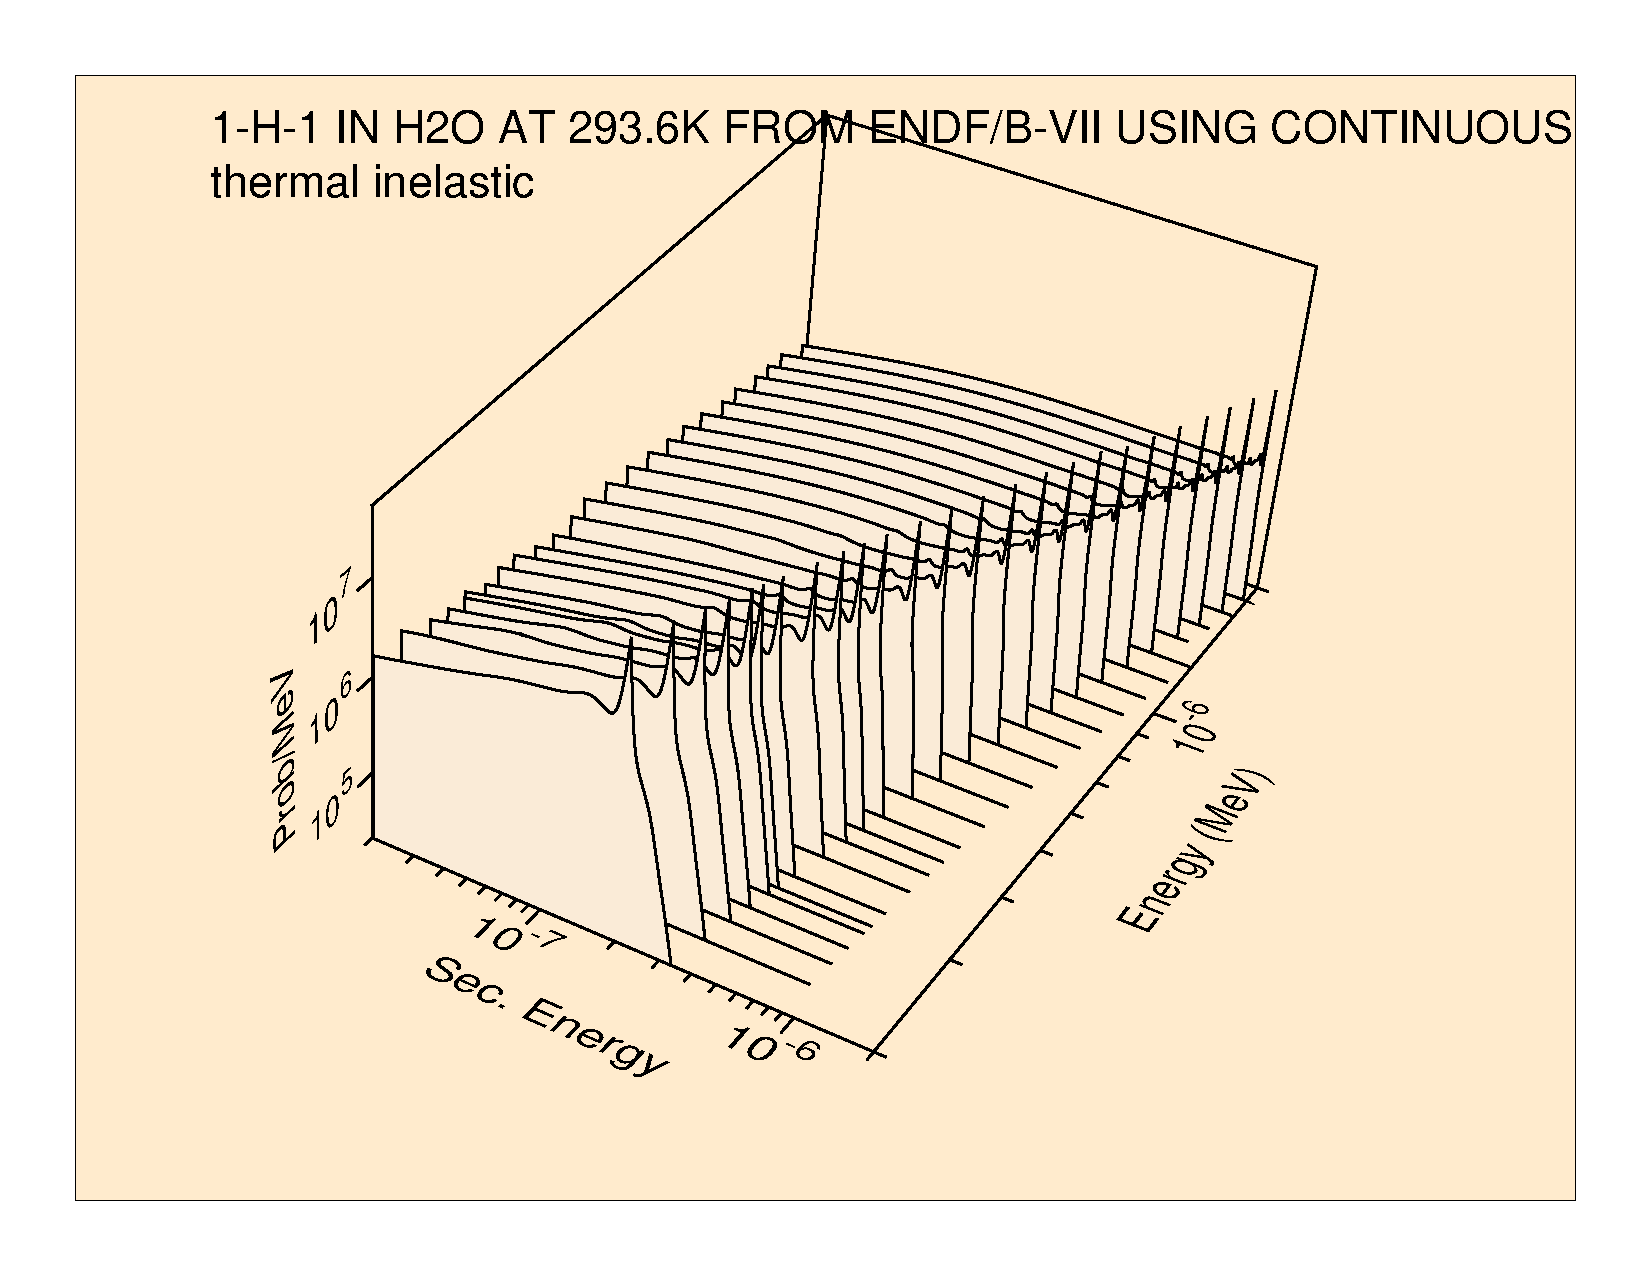
\includegraphics[keepaspectratio, height=3.5in, angle=0]{figs/thermr5ack}
\caption[Incoherent inelastic distribution for H-H$_2$O (expanded view)]
 {Expanded view of the high-energy region for the incoherent inelastic
 distribution of hydrogen bound in water.  Note the sharp quasi-elastic
 peak at $E{=}E'$.}
\label{water}
\end{figure}

A calculation of both free and graphite cross sections for ENDF/B-VII
carbon would go as follows:

\small
\begin{ccode}

 reconr
 20 22 / tape20 is carbon
 /
 600 1/
 .001/
 '6-C-nat from ENDF/B-VII'/
 0/
 broadr
 20 22 23/
 600 1/
 .001/
 293.6/
 0/
 thermr
 0 23 24/
 0 600 8 1 2 0 0 1 221 0/
 293.6/
 .005 5/
 thermr
 26 24 25 / tape 26 is ENDF/B-VII graphite
 31 600 8 1 2 1 0 1 229 0/
 293.6/
 .005 5/
 stop

\end{ccode}
\normalsize

\noindent
First, ENDF/B-VII carbon must be mounted on unit 20.  At LANL
this is done by copying it to a file named \cword{tape20} in the
user's local file space.  Similarly,  ENDF/B-VII graphite must be copied
to \cword{tape26}.  Next, \hyperlink{sRECONRhy}{RECONR} is run
to linearize the evaluation, and \hyperlink{sBROADRhy}{BROADR}
is run to prepare 293.6K cross sections.  The first THERMR
run is for free-gas scattering (\cword{mtref}=221), and the second run
is for carbon bound in graphite (\cword{mtref}=229).  Note that
\cword{natom} is now 1, and that 8 discrete angles were requested
in both cases.   For graphite, \cword{icoh} is set to 1 in order to
request the calculation of coherent elastic scattering like that shown
in Fig.~\ref{cohfig}.  The coherent results will use MF=3 and MT=230.
Distributions will be calculated to 0.5\% accuracy for energies up
to 5 eV.  The final PENDF file will be \cword{tape25}.

\subsection{Error Messages}
\label{ssTHERMR_msg}

\begin{description}
\begin{singlespace}

\item[\cword{error in thermr***nin=0}] ~\par
  An input PENDF tape is required.

\item[\cword{error in thermr***mode conversion not allowed}] ~\par
  \cword{nin} and \cword{nout} must both be binary or both be coded.

\item[\cword{error in thermr***illegal reference mt}] ~\par
  Restricted to MT=221--250.  User's should note that Card 2 has an
additional input parameter, \cword{iform}, beginning with
NJOY2012.  Unmodified NJOY99 input decks will produce this error message.

\item[\cword{error in thermr***desired material not on pendf tape}] ~\par
  Check input instructions against contents of thermal tape.

\item[\cword{error in thermr***desired temperature not on tape}] ~\par
  Check input instructions against contents of thermal tape.

\item[\cword{error in rdelas***too much elastic data}] ~\par
  There is not enough space in the allocatable array \cword{a}.
  See \cword{na}=10000.

\item[\cword{error in rdelas***desired temp not found}] ~\par
  The temperatures requested in THERMR must be the same as
  the temperatures on the input PENDF tape.

\item[\cword{error in coh***too many legendre orders}] ~\par
  The code currently computes only P$_0$, but \cword{nl}=1
  in \cword{coh} can be changed if desired.  Code is currently limited
  to 6 (P$_5$).  If more coefficients are desired, increase \cword{nlmax}
  and the dimensions of the variables \cword{s}, \cword{ej}, and \cword{ex}
  in \cword{coh}, \cword{calcem}, and \cword{tpend}.

\item[\cword{error in sigcoh***storage exceeded}] ~\par
  Not enough room for lattice factors.  Increase \cword{nw} which is
  currently 10000.

\item[\cword{error in sigcoh***illegal lat}] ~\par
  Only three lattices are coded so far.  To add others, insert the
  constants in \cword{sigcoh} and form factor formulas in \cword{form}.

\item[\cword{error in iel***bad temperature for debye-waller factor}] ~\par
  Shouldn't occur unless new materials are added incorrectly.

\item[\cword{error in iel***unknown material identifier}] ~\par
  Only three options are coded so far.  To add others, insert data
  statements for the Debye-Waller integrals and values for the
  bound cross sections.

\item[\cword{error in calcem***nl too large for binning}] ~\par
  Increase the value of the parameter \cword{nlmax} which is currently 33.

\item[\cword{error in calcem***storage exceeded}] ~\par
  There is not enough space in the global scratch array. Increase
  \cword{nwscr}, which is currently 99000, in \cword{thermr}.

\item[\cword{error in calcem***desired temperature not found}] ~\par
  Any temperature requested in THERMR must be on the input
  PENDF tape.

\item[\cword{error in calcem***bad temperature for teff}] ~\par
\item[\cword{error in calcem***bad temperature for teff2}] ~\par
  Data for effective temperatures use a temperature grid that
  is not consistent with the $S(\alpha,\beta)$ data.

\item[\cword{error in calcem***isabt=1 pendf tape found}] ~\par
  THERMR cannot process this format.

\item[\cword{error in calcem***only 2 sct atoms allowed}] ~\par
  For mixed moderators, such as BeO and Benzine, the SCT contribution
  from each atom must be included.  The code only allows for 2.

\item[\cword{error in calcem***too many angles}] ~\par
  For $E$-$\mu$-$E'$ ordering, there are more than \cword{mumax}=300
  angles being generated.

\item[\cword{error in sig***illegal option}] ~\par
 Only tabulated $S(\alpha,\beta)$ and free gas are coded at this time.

\item[\cword{error in sigl***no legal solution}]
\item[\cword{message from sigl---disc=-ffff, set to abs value....}]
\item[\cword{error in sigl***no legal solution (quadratic path)}] ~\par
  The code has trouble solving the equation for the boundary of a bin.

\item[\cword{error in tpend***storage exceeded}] ~\par
  Increase \cword{nwscr} in \cword{thermr}.

\item[\cword{error in tpend***cross section = 0}] ~\par
  Thermal cross section of zero cannot be used to normalize
  the distribution.

\end{singlespace}
\end{description}

\subsection{Input/Output Units}
\label{ssTHERMR_IOunits}

The following logical units are used.

\begin{list}{}{\leftmargin=.75in\labelsep=.25in\labelwidth=.5in}
\begin{singlespace}

\item[10/11] \cword{iold/inew} in \cword{thermr}.  Also used in
   \cword{coh}, \cword{calcem}, and \cword{tpend}.  Used for the
   \cword{loada/finda} scratch file that saves the energy grid
   and reaction cross sections.
\item[12]  \cword{nscr} in \cword{thermr}.  Also used in \cword{calcem}
   and \cword{tpend}.  Contains the scattering matrix before normalization.
\item[13]  \cword{nscr2} in \cword{thermr} and \cword{tpend}.  Contains
   data from \cword{nin} that are to be simply copied to \cword{nout}.
\item[20-99]  User's choice for \cword{nendf}, \cword{nin}, \cword{nout},
   and \cword{nread} (\cword{iinc}=2 only) to link with other modules.
   No mode conversion between \cword{nin} and \cword{nout} allowed.

\end{singlespace}
\end{list}

Units 10 and 11 are always binary.  Units 12 and 13 have the same mode
as \cword{nin} and \cword{nout}.  The user can choose the modes for
\cword{nendf}, \cword{nin}, \cword{nout}, except \cword{nin} and
\cword{nout} must have the same mode.

\subsection{Storage Allocation}
\label{ssTHERMR_storage}

The storage allocated in THERMR is for the \cword{loada/finda}
buffers and a scratch array.   The value of \cword{nbuf} my be changed
at will; larger values increase I/O efficiency.  The variable \cword{nwscr}
controls the maximum size of the TAB1 records of $\sigma(E\rightarrow E')$
versus $E'$ for incoherent scattering.  Hence it interacts with \cword{tol}.
The linearization stack (\cword{stk}) in \cword{coh} is controlled by
\cword{imax} and the number of Legendre components requested (always 1
in the standard version).  The current value of \cword{imax} (20) is
sufficient to divide each panel into parts as small as one-millionth
of the panel size.  The length of the list of lattice factors (\cword{fl})
in \cword{sigcoh} is controlled by the size of the ENDF/B File 7, and
\cword{nw}=10000 must be big enough for the problem.

\cleardoublepage


\section{GROUPR}
\label{sGROUPR}

\hypertarget{sGROUPRhy}{GROUPR}
\index{GROUPR|textbf} computes group-to-group scattering matrices, and
anisotropic photon production matrices for neutrons from ENDF/B-IV and
later evaluated nuclear data.  With ENDF-6
format files, photonuclear data and incoming and outgoing charged
particles can also be handled.  Special features are provided for
ratio quantities (for example, $\overline\mu$, $\overline\nu$, or
photon yield), inverse velocity\index{inverse-velocity},
delayed neutron spectra by time group\index{delayed-neutron spectra},
and anisotropic thermal neutron scattering.  Fission is represented as
a group-to-group matrix for full generality.  Scattering matrices
and photon production matrices may be self-shielded if desired.

The Bondarenko narrow-resonance weighting
scheme\cite{Bondarenko} is normally
used.\index{Bondarenko method}\index{narrow resonances}  Optionally,
a weighting flux can be computed for various mixtures
of heavy absorbers with light moderators.\index{flux calculator}
An accurate pointwise solution of the integral slowing down equation
is used.  This option is normally called on to account for
intermediate resonance effects in the epithermal range.
\index{epithermal}
\index{intermediate resonances}

Neutron data and photon-production data are processed in a parallel
manner using the same weight function and quadrature scheme.  This
assures consistent cross sections for coupled neutron-photon
problems.  Two-body scattering is computed with a center-of-mass (CM)
Gaussian quadrature, which gives accurate results even for small Legendre
components of the group-to-group matrix.

User conveniences include free-form input and complete control over
which reactions are processed.  The neutron group structure, photon group
structure, and weight function can each be read in or set to one of
the internal options.  Output can be printed and/or written to an
output ``groupwise-ENDF'' (GENDF)\index{GENDF} file for further processing
by a formatting module (\hyperlink{sDTFRhy}{DTFR}\index{DTFR},
\hyperlink{sCCCCRhy}{CCCCR}\index{CCCCR},
\hyperlink{sMATXSRhy}{MATXSR}\index{MATXSR},
\hyperlink{sWIMSRhy}{WIMSR}\index{WIMSR}), by the covariance module
(\hyperlink{sERRORRhy}{ERRORR})\index{ERRORR}, or by the MCNP
continuous-energy Monte Carlo
module (\hyperlink{sACERhy}{ACER})\index{ACER}.

This chapter describes the GROUPR module in NJOY2016.0.

\subsection{Multigroup Constants}
\label{ssGROUPR_MG}

Multigroup constants are normally used by computer codes that calculate
the distributions of neutrons and/or photons in space and energy, and that
compute various responses to these distributions, such as criticality,
dose to personnel, or activation of materials.  These distributions are
solutions of the neutral particle transport equation.\footnote
{The following development uses a notation based on Bell and
Glasstone\cite{ref5}, where the lower-case sigma is used for both
macroscopic and microscopic cross sections, depending on the context.
One-dimensional slab geometry is used throughout for simplicity. }

  \begin{eqnarray}
    \mu{{\partial}\over{\partial x}}\phi(x,\mu,E)
    &+&\sigma_t(x,E)\,\phi(x,\mu,E)\nonumber\\
    &=&\int d{\bf\Omega}'\int dE'\,\sigma_X(x,E'{\rightarrow}E,
    {\bf\Omega}'{\rightarrow}{\bf\Omega})
    \,\phi(x,\mu',E')\nonumber\\
    &+&Q(x,\mu,E) \,\,,
  \label{Eq1}
  \end{eqnarray}

\noindent
where the flux $\phi$ is allowed to vary with position $x$, direction
${\bf\Omega}$ with polar cosine $\mu$, and energy $E$.  Similarly, the
macroscopic total cross section $\sigma_t$ varies with position and
energy.  The right-hand side of the equation contains the source due to
transfers from other directions ${\bf\Omega}'$ and energies $E'$ (as
described by the macroscopic transfer cross section $\sigma_X$), and
a fixed or external source $Q$.

The macroscopic cross sections (in units of cm$^{-1}$) in Eq.~\ref{Eq1}
can be calculated from microscopic cross sections for the component
isotopes or elements (in barns) using

  \begin{equation}
    \sigma_t(x,E)=\sum_i\rho_i(x)\,\sigma_t^i(T[x],E) \,\,,\\
  \end{equation}

\noindent
where $\rho_i$ is the number density for a constituent (in
barns$^{-1}$cm$^{-1}$), which may vary with position, and T is the
temperature, which may also vary with position.  A similar formula
holds for $\sigma_X$.

The transfer cross section $\sigma_X$ (which includes both scattering
and fission processes) is normally assumed to depend only on the cosine
of the scattering angle, $\mu_0={\bf\Omega}\cdot{\bf\Omega}'$.  This
allows $\sigma_X$ to be expanded using Legendre polynomials

  \begin{equation}
    \sigma_X(x,E'{\rightarrow}E,
    {\bf\Omega}'{\rightarrow}{\bf\Omega})=
    \sum_{\ell=0}^{\infty}
    {{2\ell+1} \over 4\pi}\,\sigma_{X\ell}(x,E'{\rightarrow}
    E)\,P_\ell(\mu_0)\,\,.\\
  \end{equation}

\noindent
Application of the addition theorem and integration over azimuthal angle
then gives

  \begin{eqnarray}
    \mu{{\partial}\over{\partial x}}\phi(x,\mu,E)&+&\sigma_t(x,E)
    \,\phi(x,\mu,E)\nonumber\\
    &=& \sum_{\ell=0}^{\infty}{{2\ell+1}\over 2}
    P_{\ell}(\mu)\int\sigma_{X\ell}(x,E'{\rightarrow}E)
    \,\phi_{\ell}(x,E')\,dE'\nonumber\\
    &+&Q(x,\mu,E)\,\,,
  \label{Eq4}
  \end{eqnarray}

\noindent
where

  \begin{equation}
    \phi_\ell(x,E)=\int P_\ell(\mu) \,\phi(x,\mu,E)\,d\mu\,\,.
  \end{equation}

\noindent
The desired responses are then given by

  \begin{equation}
    R(x)=\int\sigma_r(x,E)\,\phi_0(x,E)\,dE\,\,,
  \label{Eq6}
  \end{equation}

\noindent
where $\sigma_r$ is the reaction cross section for the response.  The next
step is to integrate Eqs.~\ref{Eq4} and \ref{Eq6} over a range of
energies chosen to lie in group $g$.  The results are

  \begin{eqnarray}
    \mu{{\partial}\over\partial x}\phi_g(x,\mu)&+&
    \sum_{\ell=0}^{\infty}P_{\ell}(\mu)\,\sigma_{t\ell g}(x)
    \,\phi_{\ell g}(x)\nonumber\\
    &=& \sum_{\ell=0}^{\infty}{{2\ell+1}\over 2}P_{\ell}(\mu)
    \sum_{g'}\sigma_{X\ell g'\rightarrow g}(x)\,\phi_{\ell g'}(x)
    +Q_g(x,\mu)\,\,,
  \label{Eq7}
  \end{eqnarray}

\noindent
and

  \begin{equation}
    R(x)=\sum_g\sigma_{rg}(x)\,\phi_{0g}(x)\,\,,
  \end{equation}

\noindent
where

  \begin{equation}
    \phi_{\ell g}(x)=\int_g\phi_{\ell}(x,E)\,dE\,\,,
  \end{equation}

  \begin{equation}
    \sigma_{t\ell g}(x)={\displaystyle{\int_g
    \sigma_t(x,E)\,\phi_{\ell}(x,E)\,dE}
    \over\displaystyle {\int_g\phi_{\ell}(x,E)\,dE}}\,\,,
  \label{Eq10}
  \end{equation}

  \begin{equation}
    \sigma_r(x)={\displaystyle{\int_g\sigma_r(x,E)\,\phi_0(x,E)\,dE}
    \over\displaystyle {\int_g\phi_0(x,E)\,dE}}\,\,,
  \label{Eq11}
  \end{equation}

\noindent
and
  \begin{equation}
    \sigma_{X\ell g'\rightarrow g}={\displaystyle{\int_gdE\int_{g'}
    dE'\,\sigma_{X\ell}(x,E'{\rightarrow}E)\,\phi_{\ell}(x,E)}
    \over \displaystyle{\int_g\phi_{\ell}(x,E)\,dE}}\,\,.
  \label{Eq12}
  \end{equation}

The last three equations provide the fundamental definitions for the
multigroup cross sections\index{multigroup cross sections} and the
group-to-group matrix\index{group-to-group matrices}.  Note that
the values of the group constants depend upon the basic energy-dependent
cross sections obtained from an ENDF-format evaluation by way of
the \hyperlink{sRECONRhy}{RECONR}\index{RECONR},
\hyperlink{sBROADRhy}{BROADR}\index{BROADR},
\hyperlink{sUNRESRhy}{UNRESR}\index{UNRESR},
\hyperlink{sHEATRhy}{HEATR}\index{HEATR},
\hyperlink{sTHERMRhy}{THERMR}\index{THERMR},
and \hyperlink{sPURRhy}{PURR}\index{PURR} modules
of NJOY, and the shape of $\phi$ within the group.

\subsection{Group Ordering}
\label{ssGROUPR_Group_Order}

Since neutrons normally lose energy in scattering, the scattering source
into group $g$ depends on the flux at higher-energy groups $g'$ and the
cross section for transferring neutrons from $g'$ to $g$.  For this
reason, Eq.~\ref{Eq7} is usually solved by sweeping from high energies
to low energies.  (Any thermal upscatter or fission is handled by
iteration.)  Data libraries for use with transport codes normally number
the groups such that group 1 is the highest-energy group, and all the
scattering matrix elements that transfer neutrons into group 1 are given
first, followed by those for scattering into group 2, and so on.

However, in ENDF files the evaluated nuclear data are always given in
order of increasing incident energy, and secondary neutron distributions
are described by giving emission spectra for given incident energies.
Therefore, GROUPR numbers its groups such that group 1 is the
lowest-energy group, and it calculates that scattering out of group 1,
followed by the scattering out of group 2, and so on.

The ``backward'' energy-group numbering convention used by GROUPR is a
possible source of confusion in interpreting output produced by the
various modules of NJOY.  All group indices printed by GROUPR or written
to the GROUPR output file use the increasing-energy order.  The
covariance modules and photon interaction module follow the GROUPR
ordering convention.  Output modules such as
\hyperlink{sDTFRhy}{DTFR}, \hyperlink{sCCCCRhy}{CCCCR},
\hyperlink{sMATXSRhy}{MATXSR}, and \hyperlink{sWIMSRhy}{WIMSR}
invert the group order and rearrange the scattering matrices from
the GROUPR outscatter organization to the ``transport'' inscatter form.
Any group indices printed by these three output modules will be in the
conventional transport decreasing-energy order.

\subsection{Basic ENDF Cross Sections}
\label{ssGROUPR_BasicXS}

The basic energy-dependent cross sections and energy-angle distributions
needed for Eqs.~\ref{Eq10}, \ref{Eq11}, and \ref{Eq12} are obtained
from evaluated nuclear data in ENDF format\cite{ENDF102}.  These data
are indexed by material (MAT), type of information (MF), and reaction (MT).
Materials can be single isotopes, elements, or compounds.  Type of
information includes energy-dependent cross section (MF=3), angular
distributions (MF=4), secondary energy distributions (MF=5), and
energy-angle distributions (MF=6).  Reactions include the total (MT=1)
required for Eq.~\ref{Eq10}, the partial scattering reactions that must
be summed for Eq.~\ref{Eq12} [that is, elastic (MT=2), discrete-level
inelastic (MT=51 -- 90), (n,2n) (MT=16), {\it etc.}], and the many partial
reactions that can be used to calculate responses [for example, (n,2n)
or (n,$\alpha$) for activation, gas production, heat production (KERMA),
radiation damage (DPA), {\it etc.}].

Before using GROUPR, the basic ENDF/B cross sections should have been
converted into energy- and temperature-dependent pointwise cross sections
in PENDF\index{PENDF} (pointwise ENDF) format using
\hyperlink{sRECONRhy}{RECONR}\index{RECONR} and
\hyperlink{sBROADRhy}{BROADR}\index{BROADR}.  For heavy
isotopes, unresolved self-shielding
data should have been added to the PENDF tape\footnote{
  The term ``tape'' is used loosely in this report to refer
  to any input or output file.  Of course, such files would
  be on disk storage in a modern system.}
using \hyperlink{sUNRESRhy}{UNRESR}\index{UNRESR} or
\hyperlink{sPURRhy}{PURR}\index{PURR}.  If requested, heat production
cross sections (KERMA)\index{KERMA}, radiation damage production
(or DPA)\index{DPA}, and thermal upscatter data can also have been
added to the PENDF tape using \hyperlink{sHEATRhy}{HEATR}\index{HEATR}
and \hyperlink{sTHERMRhy}{THERMR}\index{THERMR}.
See the chapters on these other modules for more information.

The detailed methods used for evaluating Eqs.~\ref{Eq10}, \ref{Eq11},
and \ref{Eq12} from ENDF and PENDF tapes are given below (see
Sections~\ref{ssGROUPR_GrpInt} through \ref{ssGROUPR_F6_EA}).  An
 example of an ENDF pointwise cross section compared with group-averaged
 cross sections from GROUPR is given in Fig.~\ref{gr1}.

\begin{figure}[thb]\centering
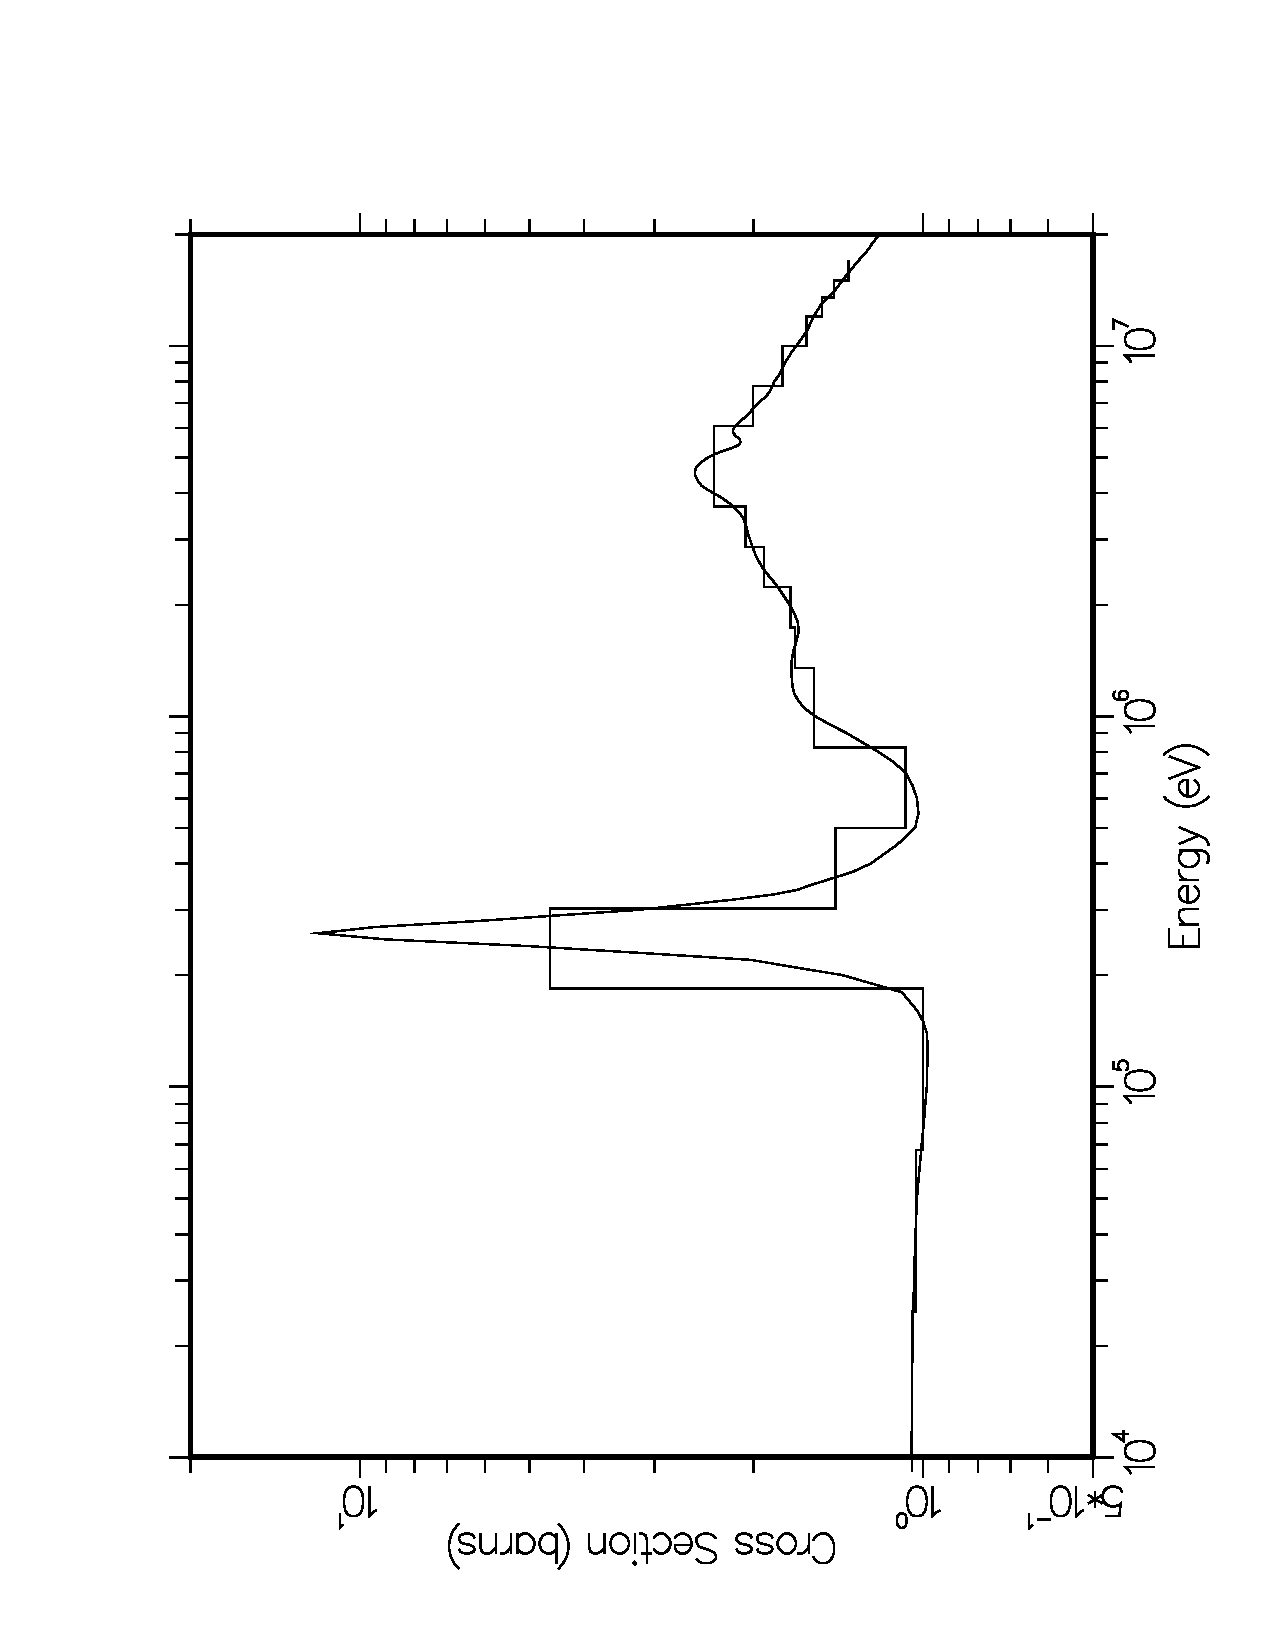
\includegraphics[keepaspectratio, height=3.5in, angle=270]{figs/groupr1ack}
\caption[Pointwise and multigroup cross section comparison]{A comparison
 of the pointwise and multigroup representations for the total cross section of
 $^{7}$Li.  The Los Alamos 30-group structure is shown.}
\label{gr1}
\end{figure}

\subsection{Weighting Flux}
\label{ssGROUPR_WtFlux}

In general, the weighting flux\index{weighting flux} $\phi$ is not
known; it is, after all, the particle distribution being sought
in the transport calculation.  However, it is often possible
to obtain fairly accurate group constants for a particular
application if the shape of the flux is reasonably well known
over the broad energy ranges of a particular few-group structure
(for example, a fission spectrum, thermal Maxwellian, or $1/E$
slowing-down spectrum). Alternatively, one can use many small groups
so that mistakes in guessing the shape inside the group are not very
important.  The key to using the multigroup method effectively is
balancing the tradeoffs between the choice of weight function and
the number of groups used for each different class of problem being solved.

In many cases of practical interest, the flux $\phi$ will contain dips
corresponding to the absorption resonances of the various materials.
In the reaction rate $\sigma(E)\times\phi(E)$, these dips clearly reduce
(self-shield) the effect of the corresponding resonance.  GROUPR provides
two methods to estimate the effect of this self-shielding: the Bondarenko
model and the flux calculator.
\index{self-shielding}
\index{Bondarenko method}
\index{flux calculator}

In the Bondarenko model\cite{Bondarenko}, the narrow resonance (NR)
approximation\index{narrow resonance approximation}, and the
B$_{\rm N}$ approximation for large systems\cite{ref5} are invoked
to obtain

  \begin{equation}
    \phi_{\ell}(E)={{W_{\ell}(E)}\over{[\sigma_t(E)]^{\ell+1}}}\,\,,
  \end{equation}

\noindent
where $\phi_{\ell}$ is the $\ell$-th Legendre component of the angular
flux, the $W_\ell(E)$ are smooth functions of energy (such as $1/E$+fission),
and $\sigma_t(E)$ is the total macroscopic cross section for the material.
GROUPR takes all of the $W_{\ell}$ to be equal to the single function $C(E)$,
where $C(E)$ can be read in or set to one of several internally defined
functions.  It is further assumed that the important self-shielding effect
of the flux can be obtained for isotope $i$ by representing all the other
isotopes with a constant ``background cross section'', $\sigma_0$.  Therefore,
\index{background cross section}
\index{$\sigma_0$}

   \begin{equation}
    \phi_{\ell}^i(E)={{C(E)}\over
    {[\sigma_t^i(E)+\sigma_0^i]^{\ell+1}}} \,\,,
  \label{Eq14}
  \end{equation}

\noindent
where $\sigma_t^i$ is the microscopic total cross section for isotope $i$.
The qualitative behavior of Eq.~\ref{Eq14} is easy to understand.
If $\sigma_0$ is larger than the tallest peaks in $\sigma_t$, the weighting
flux $\phi$ is approximately proportional to the smooth weighting function
$C(E)$.  This is called infinite dilution\index{infinite dilution};
 the cross section in the material of interest has little or no effect
on the flux.  On the other hand, if $\sigma_0$ is small with respect
to $\sigma_t$, the weighting flux will have large dips at the locations
of the peaks in $\sigma_t$, and a large self-shielding effect will
be expected.

Each component material of a mixture has a different weight function.
The macroscopic total cross sections are given by

  \begin{equation}
    \sigma_{t\ell g}=\sum_i \rho_i \,\sigma_{t\ell g}^i(\sigma_0^i,T)\,\,,
  \end{equation}

\noindent
where

  \begin{equation}
    \sigma_{t\ell g}^i(\sigma_0,T)=
    {{\displaystyle\int_g {{\sigma_t^i(E,T)}\over
    {[\sigma_0+\sigma_t^i]^{\ell+1}}}
    C(E)\,dE}\over
    {\displaystyle\int_g{{1}\over
    {[\sigma_0+\sigma_t^i]^{\ell+1}}} C(E)\,dE}}\,\,.
  \end{equation}

\noindent
Similar equations are used for $\sigma_R$ and $\sigma_{X\ell g\rightarrow g'}$.
On the GROUPR level, $\sigma_0$ and $T$ are simply parameters.  Subsequent
codes, such as 1DX\cite{1DX}\index{1DX} or TRANSX\cite{TRANSX,TRANSX2},
\index{TRANSX} can compute an appropriate value for $\sigma_0$, and then
interpolate in tables of cross section versus $\sigma_0$ and $T$ to get
the desired self-shielded group constants.

The appropriate value for $\sigma_0^i$\index{$\sigma_0$} is obvious
when a single resonance material is mixed with a moderator material
(for example, $^{238}$UO$_2$), because the admixed materials typically
have a constant cross section in the energy range where the heavy isotopes
have resonances.  For a mixture of resonance materials, the normal procedure
is to preserve the average of Eq.~\ref{Eq14} in each group by using

  \begin{equation}
    \sigma_{0g}^i={{1}\over{\rho_i}}
    \sum_{j\ne i}\rho_j \,\sigma_{t0g}^j(\sigma_{0g}^j,T)\,\,,
  \label{Eq17}
  \end{equation}

\noindent
where the $\rho_i$ are atomic densities or atomic fractions.
Eq.~\ref{Eq17} is solved by iteration.  Interference between resonances
in different materials is handled in an average sense only.

In the unresolved energy range\index{unresolved resonance range}
(see \hyperlink{sUNRESRhy}{UNRESR}\index{UNRESR} and
\hyperlink{sPURRhy}{PURR}\index{PURR}), the explicit dependence
of cross section on energy is not known.  The integrands are replaced
by their expected values

  \begin{equation}
    \sigma_{x\ell g}(\sigma_0)=
    {\displaystyle{\int_g\biggl<{{\sigma_x}\over{[\sigma_0+\sigma_t]^{\ell+1}}}
    \,\biggr>W_{\ell}\,dE}
    \over\displaystyle{\int_g\biggl<{1\over{[\sigma_0+\sigma_t]^{\ell+1}}}
    \,\biggr>W_{\ell}\,dE}}\,\,,
  \label{Eq18}
  \end{equation}

\noindent
where the expected values are averages over the distributions of
resonance position and width expected in the vicinity of energy $E$.
The \hyperlink{sUNRESRhy}{UNRESR} and \hyperlink{sPURRhy}{PURR}
modules produce effective self-shielded point
cross sections defined by

  \begin{equation}
    \bigl<\sigma_x\bigr>_{\ell}=
    {{\displaystyle{\biggl<{{\sigma_x}\over{[\sigma_0
    +\sigma_t]^{\ell+1}}}}\biggr>}
    \over\displaystyle{\biggl<
    {1\over{[\sigma_0+\sigma_t]^{\ell+1}}}\biggr>}}\,\,.
  \label{Eq19}
  \end{equation}

\noindent
Substituting Eq.~\ref{Eq19} into Eq.~\ref{Eq18} gives an equation of
the form of Eqs.~\ref{Eq10} and \ref{Eq11}, except that $\sigma$ is
replaced by $\bigl<\sigma\bigr>$, and the flux is replaced by an average
effective flux.  This effective flux can be obtained by manipulating the
effective total cross section as follows:

  \begin{equation}
    \bigl<\sigma_t\bigr>_{\ell}=
    {\displaystyle{\biggl<{{\sigma_0+\sigma_t-\sigma_0}
    \over{[\sigma_0+\sigma_t]^{\ell+1}}}\biggr>}
    \over\displaystyle{\biggl<{{1}\over
    {[\sigma_0+\sigma_t]^{\ell+1}}}\biggr>}}
    ={\displaystyle{\biggl<{1
    \over{[\sigma_0+\sigma_t]^{\ell}}}\biggr>}
    \over\displaystyle{\biggl<{{1}\over
    {[\sigma_0+\sigma_t]^{\ell+1}}}\biggr>}}-\sigma_0\,\,,
  \end{equation}

\noindent
from which

  \begin{equation}
    \biggl<{{1}\over{[\sigma_0+\sigma_t]^{\ell+1}}}\biggr>
    = {\displaystyle{\biggl<{{1}\over{[\sigma_0+\sigma_t]^{\ell}}}\biggr>}
    \over{\sigma_0+\bigl<\sigma_t\bigr>_k}}\,\,.
  \label{Eq21}
  \end{equation}

\noindent
Eq.~\ref{Eq21} defines a recursion relation which can be used to compute
the effective flux to any order

  \begin{equation}
    \biggl<{{1}\over{[\sigma_0+\sigma_t]^{\ell+1}}}\biggr>
    = \prod_{k=0}^{\ell}{1\over{\sigma_0+\bigl<\sigma_t\bigr>_k}}\,\,,
  \label{Eq22}
  \end{equation}
\vspace{0.5 pt}

\noindent
This equation reduces to Eq.~\ref{Eq14} in the resolved range.  It is
the formula used in \cword{genflx} to compute $\phi_{\ell}(E)$ for the
Bondarenko option.

When heterogeneity\index{heterogeneity} effects are important, the
background cross section method can be extended as follows.  In an
infinite system of two regions (fuel and moderator), the neutron
balance equations are

  \begin{equation}
    V_f\sigma_f\phi_f=(1-P_f)V_f S_f+P_m V_m S_m\,\,,
  \end{equation}

\noindent
and

  \begin{equation}
    V_m\sigma_m\phi_m=P_f V_f S_f+(1-P_m)V_m S_m\,\,,
  \end{equation}

\noindent
where $V_f$ and $V_m$ are the region volumes, $\sigma_f$ and $\sigma_m$
are the corresponding total macroscopic cross sections, $S_f$ and $S_m$
are the sources per unit volume in each region, $P_f$ is the probability
that a neutron born in the fuel will suffer its next collision in the
moderator, and $P_m$ is the probability that a neutron born in the
moderator will suffer its next collision in the fuel.  As usual, use
is made of the reciprocity theorem,
\index{reciprocity theorem}

  \begin{equation}
    V_f\sigma_f P_f=V_m\sigma_m P_m \,\,,
  \end{equation}

\noindent
and the Wigner rational approximation\index{Wigner rational approximation}
to the fuel escape probability,

  \begin{equation}
    P_f={{\sigma_e}\over{\sigma_e+\sigma_f}}\,\,,
  \end{equation}

\noindent
where $\sigma_e$ is a slowly varying function of energy called the escape
cross section\index{escape cross section}, to obtain an equation for the
fuel flux in the form

  \begin{equation}
    (\sigma_f+\sigma_e)\phi_f={{\sigma_e S_m}\over \sigma_m} +S_f \,\,.
  \label{Eq27}
  \end{equation}

\noindent
In the limit where the resonances are narrow with respect to both fuel
and moderator scattering, the source terms $S_f$ and $S_m$ take on their
asymptotic forms of $\sigma_p/E$ and $\sigma_m/E$ respectively, and this
equation becomes equivalent to the Bondarenko model quoted above with

  \begin{equation}
    \sigma_0^f={\sigma_e \over \rho_f}\,\,,
  \label{Eq28}
  \end{equation}

\noindent
and

  \begin{equation}
    C(E)={{\sigma_e+\sigma_p}\over{\rho_f E}}\,\,.
  \end{equation}

\noindent
Note that a large escape cross section (a sample that is small relative
to the average distance to collision), corresponds to infinite dilution
as discussed above.  To illustrate the general case, consider a neutron
traveling through a lump of uranium oxide with an energy close to a
resonance energy.  If the neutron scatters from an oxygen nucleus, it
will lose enough energy so that it can no longer react with the uranium
resonance.  Similarly, if the neutron escapes from the lump, it can no
longer react with the uranium resonance.  The processes of moderator
scattering and escape are equivalent in some way.  Comparing
Eq.~\ref{Eq28} with Eq.~\ref{Eq17} gives an
\index{equivalence principle} ``equivalence principle''
that says that a lump of particular dimensions and a mixture of
particular composition will have the same self-shielded cross sections
when the narrow resonance approximation is valid.  The effects of
material mixing and escape can simply be added to obtain the effective
$\sigma_0$ for a lump containing admixed moderator material.  Therefore,
Eq.~\ref{Eq17} is extended to read

  \begin{equation}
    \sigma_{0g}^i ={{1} \over {\rho_i}}
    \biggl\lbrace \sigma_e +
    \sum_{j\ne i} \rho_j \,\sigma_{t0g}^j
    (\sigma_{0g}^j ,T) \biggr\rbrace \,\,,
  \end{equation}

\noindent
where the escape cross section for simple convex objects (such as plates,
spheres, or cylinders) is given by $(4V{/}S)^{-1}$, where $V$ and $S$
are the volume and surface area of the object, respectively.  Many codes
that use the background cross section method modify the escape cross section
as defined above to correct for errors in the Wigner rational
approximation (``Bell factor''\index{Bell factors},
``Levine factor'' \index{Levine factors}), or to correct for
the interaction between different lumps in the moderating region
(``Dancoff corrections'')\index{Dancoff corrections}.  These
enhancements will not be discussed here.

As an example of self-shielded cross sections and how they vary
with the background cross section, Fig.~\ref{u238ng} shows the
first three capture resonances of $^{238}$U (which are very important
for thermal power reactors) at room temperature for $\sigma_0$
values ranging from infinity down to 10 barns.  Background cross
sections that range between 20 and 50 barns are typical for
uranium-oxide pin cells.

\begin{figure}[tp]\centering
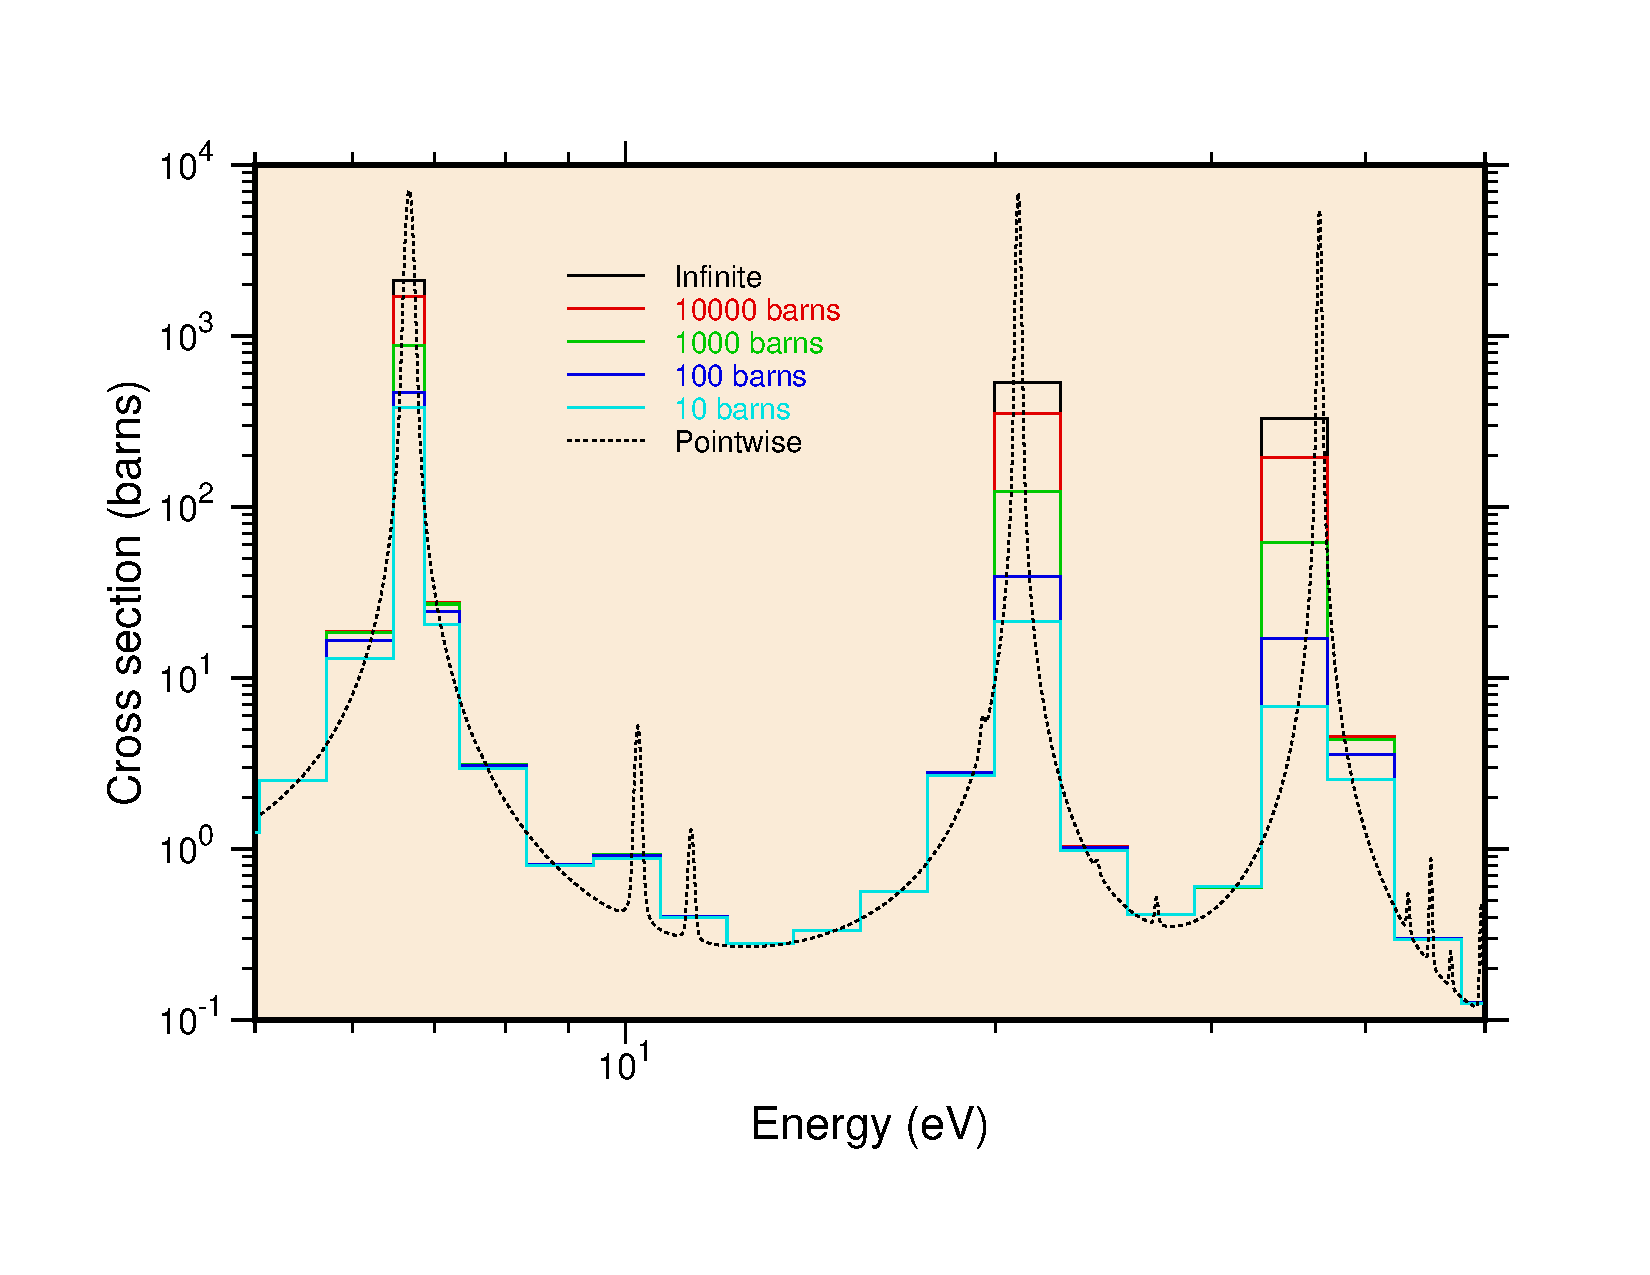
\includegraphics[keepaspectratio, height=3.2in, angle=0]{figs/u238ngack}
\caption[The self-shielding effect on the first three $^{238}$U capture
 resonances.]{The self-shielding effect on the first three $^{238}$U
 capture resonances at room temperature in the 5 to 50 eV range.  The
 multigroup boundaries are from the Los Alamos 187-group structure.}
\label{u238ng}
\end{figure}

\begin{figure}[bp]\centering
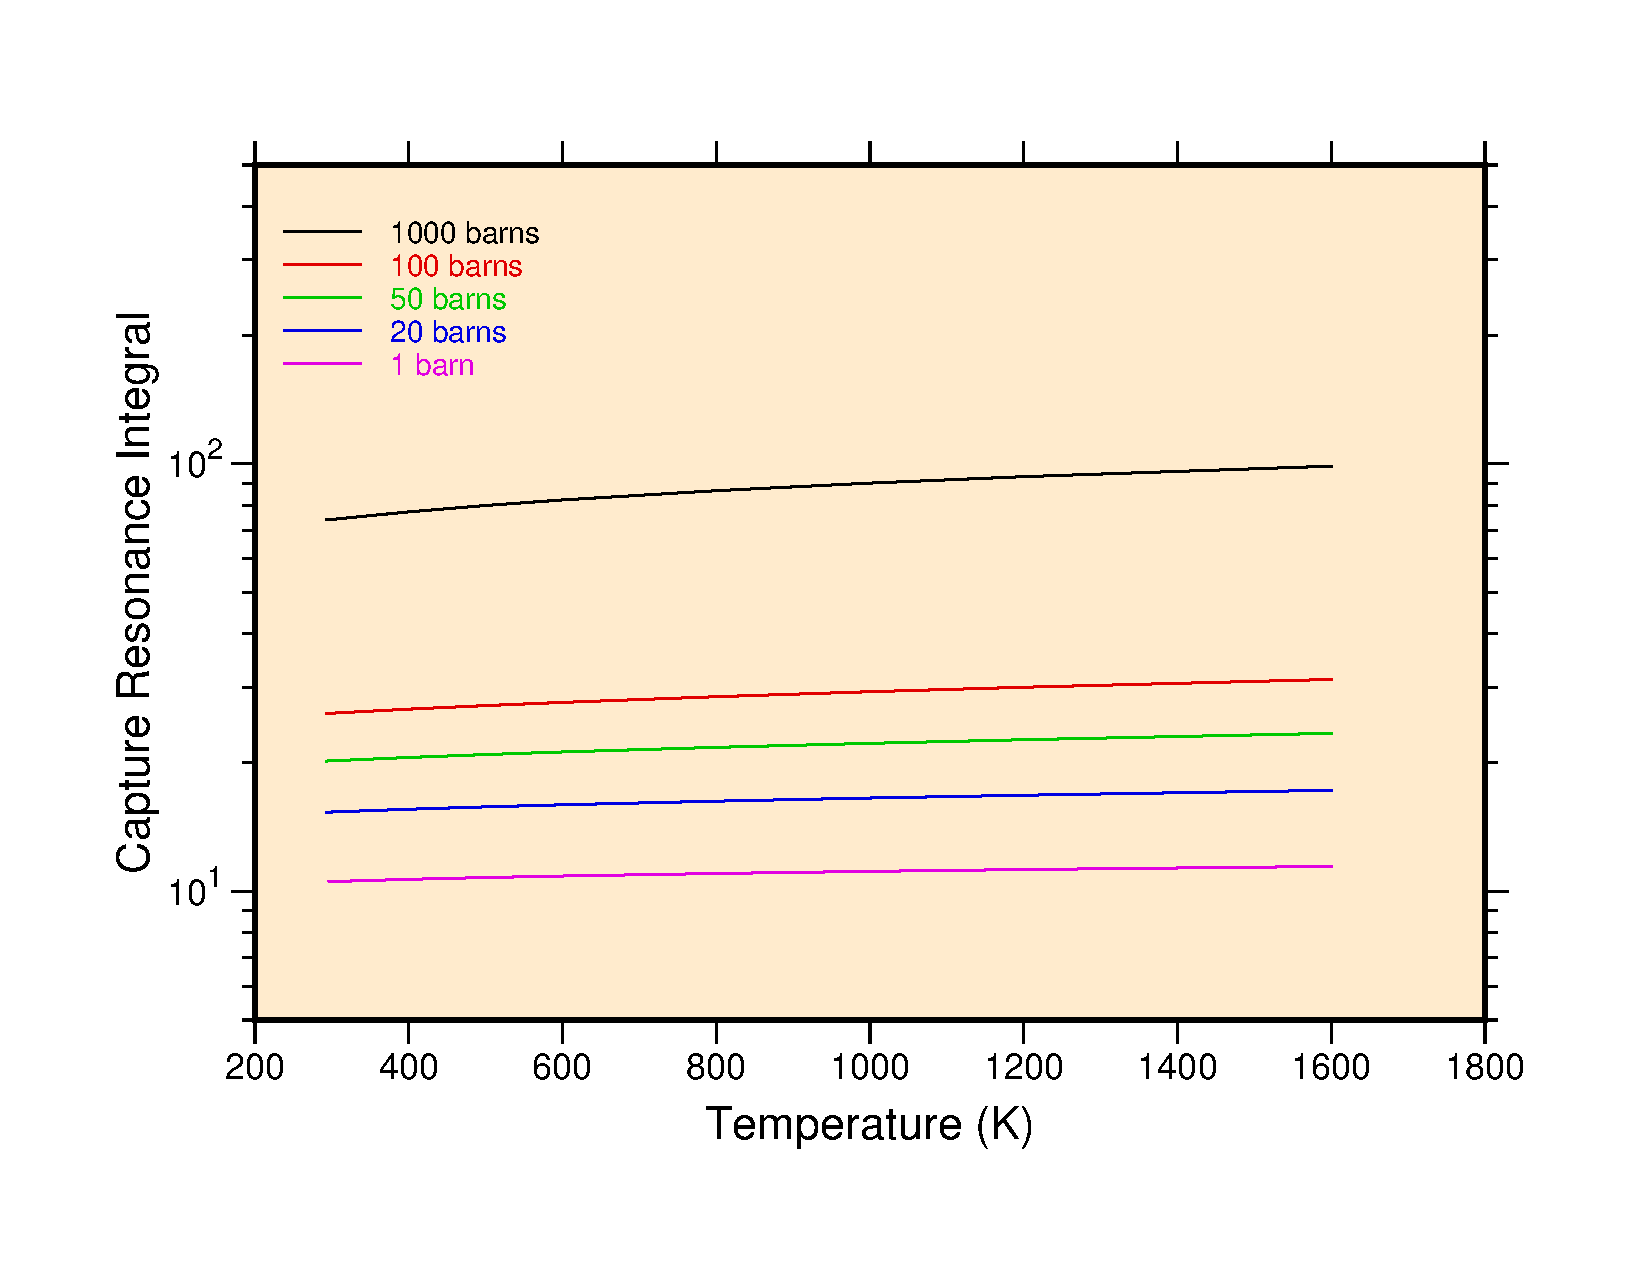
\includegraphics[keepaspectratio, height=3.2in, angle=0]{figs/u238riack}
\caption[$^{238}$U capture resonance integral versus temperature and
 background cross section]{The capture resonance integral for $^{238}$U
 showing its variation with temperature and background cross section
 $\sigma_0$.  The resonance integral at infinite dilution is 275.58 barns.  Note
 the slope with temperature, which helps to produce a negative temperature
 coefficient for uranium systems.}
\label{u238ri}
\end{figure}

The \hyperlink{sBROADRhy}{BROADR} chapter of this report
showed its capability to
compute standard resonance integrals.  However, when self shielding
and material temperature come into play, the effective resonance
integral changes.  GROUPR can calculate these quantities by doing
one-group calculations with $1/E$ weighting over a standard energy
range. Using the range 0.5 eV to the upper limit of the evaluation
will match what \hyperlink{sBROADRhy}{BROADR} does.  Fig.~\ref{u238ri}
shows the temperature
dependence of the capture resonance integral for $^{238}$U from
ENDF/B-VII at several different background cross sections.  The range between
20 and 50 barns is typical for reactor pin cells.


\subsection{Flux Calculator}
\label{ssGROUPR_FluxCalc}

This narrow-resonance approach is quite useful for practical fast
reactor problems.  However, for nuclear systems sensitive to energies
from 1 to 500 eV, there are many broad- and intermediate-width resonances
which cannot be self-shielded with sufficient accuracy using the
Bondarenko approach.  The GROUPR flux calculator\index{flux calculator}
is designed for just such problems.

Consider an infinite homogeneous mixture of two materials and assume
isotropic scattering in the center-of-mass system.  The integral
slowing-down equation becomes

  \begin{eqnarray}
    \sigma(E)\,\phi(E)&=&\int_E^{E/\alpha_1}{{\sigma_{s1}(E')}\over
    {(1-\alpha_1)E'}}\,\phi(E')\,dE'\nonumber\\
    &+&\int_E^{E/\alpha_2}{{\sigma_{s2}(E')}\over
    {(1-\alpha_2)E'}}\,\phi(E')\,dE'\,\,.
  \end{eqnarray}

\noindent
Furthermore, assume that material 1 is a pure scatterer with constant
cross section and transform to the $\sigma_0$ representation.  The
integral equation becomes

  \begin{eqnarray}
    [\sigma_0+\sigma_{t2}(E)]\,\phi(E)&=&
    \int_E^{E/\alpha_1}{{\sigma_0}\over
    {(1-\alpha_1)E'}}\,\phi(E')\,dE'\nonumber\\
    &+&\int_E^{E/\alpha_2}{{\sigma_{s2}(E')}\over
    {(1-\alpha_2)E'}}\,\phi(E')\,dE'\,\,.
  \end{eqnarray}

\noindent
Finally, assume that the moderator (material 1) is light enough so that
all the resonances of material 2 are narrow with respect to scattering
from material 1.  This allows the first integral to be approximated by
its asymptotic form, $1/E$.  More generally, the integral is assumed to
be a smooth function of $E$ given by $C(E)$.  In this way, material 1
can represent a mixture of other materials just as in the Bondarenko
method.  Fission source and thermal upscatter effects can also be lumped
in $C(E)$.  The integral equation has now been reduced to

  \begin{equation}
    [\sigma_0+\sigma_t(E)]\,\phi(E)={C(E)\,\sigma_0}
    +\int_E^{E/\alpha}{{\sigma_s(E')}\over
    {(1-\alpha)E'}}\,\phi(E')\,dE'\,\,.
  \label{Eq33}
  \end{equation}

\noindent
This is the simplest problem that can be solved using the flux calculator.
The results still depend on the single parameter $\sigma_0$, and they
can be used easily by codes that accept Bondarenko cross sections.

For heterogeneous problems, when the narrow-resonance approximation
fails, both $S_f$ and $S_m$ in Eq.~\ref{Eq27} will show resonance features.
To proceed further with the solution of this equation, it is necessary
to eliminate the moderator flux that is implicit in $S_m$.  As
a sample case, consider a fuel pin immersed in a large region of
water.  The fission neutrons appear at high energies, escape from the
pin, slow down in the moderator (giving a $1/E$ flux), and are absorbed
by the resonances in the pin.  In this limit, any dips in the moderator
flux caused by resonances in the fuel are small.  On the other hand, in
a closely packed lattice, the flux in the moderator is very similar to
the flux in the fuel, and resonance dips in the moderator flux become
very evident.  Intermediate cases can be approximated\cite{ref9} by assuming

  \begin{equation}
    \phi_m=(1-\beta)\,{C(E)}+\beta\phi_f\,\,,
  \end{equation}

\noindent
where $\beta$ is a heterogeneity parameter given by

  \begin{equation}
    \beta={{V_f\sigma_e}\over{V_m\sigma_m}}\,\,.
  \end{equation}

\noindent
Note that $\beta\rightarrow 0$ gives the isolated rod limit and
$\beta\rightarrow 1$ gives the close-packed lattice limit.  This
substitution reduces the calculation of the fuel flux to

  \begin{equation}
    (\sigma_f+\sigma_e)\,\phi_f=(1-\beta)\,
    {C(E)\,\sigma_e }+S_\beta\,\,,
  \end{equation}

\noindent
where $S_\beta$ is the source term corresponding to a homogeneous mixture
of the fuel isotopes with the isotopes from the moderator region changed
by the factor $\beta\sigma_e/\sigma_m$.  If the fuel and moderator each
consisted of a single isotope and for isotropic scattering in the
center-of-mass system, the integral equation would become

  \begin{eqnarray}
    [\sigma_0+\sigma_t(E)]\,\phi_f(E)&=&
    (1-\beta)\,{C(E)\,\sigma_0}\nonumber\\
    &+&\int_E^{E/\alpha_m}{{\beta\sigma_0}\over
    {(1-\alpha_m)E'}}\,\phi_f(E')\,dE'\nonumber\\
    &+&\int_E^{E/\alpha_f}{{\sigma_{sf}(E')} \over
    {(1-\alpha_f)E'}}\,\phi_f(E')\,dE'\,\,,
  \label{Eq37}
  \end{eqnarray}

\noindent
where $\sigma_0$ is $\sigma_e$ divided by the fuel density (units are
barns/atom), $\alpha_m$ and $\alpha_f$ are the maximum fractional
energy change in scattering for the two isotopes, and $\sigma_{sf}(E')$
is the fuel scattering cross section.

This result has a form parallel to that of Eq.~\ref{Eq33}, but the
solution depends on the two parameters $\beta$ and $\sigma_0$.  For any
given data set, $\beta$ must be chosen in advance.  This might not be
difficult if the data are to be used for one particular system, such as
pressurized water reactors.  The routine also has the capability to
include one more moderator integral with a different $\alpha$ value and
a constant cross section.  The full equation is

  \begin{eqnarray}
    [\sigma_0+\sigma_t(E)]\,\phi_f(E)&=&
    (1-\beta)\,{C(E)\,\sigma_0}\nonumber\\
    &+&\int_E^{E/\alpha_3}{{\beta(1-\gamma)(\sigma_0-\sigma_{am}}\over
    {(1-\alpha_3)E'}}\,\phi_f(E')\,dE'\nonumber\\
    &+&\int_E^{E/\alpha_2}{{\sigma_{am}+\beta\gamma(\sigma_0-\sigma_{am}}\over
    {(1-\alpha_2)E'}}\,\phi_f(E')\,dE'\nonumber\\
    &+&\int_E^{E/\alpha_f}{{\sigma_{sf}(E')} \over
    {(1-\alpha_f)E'}}\,\phi_f(E')\,dE'\,\,,
  \label{Eq37a}
  \end{eqnarray}

\noindent
where $\sigma_{am}$ is the cross section of the admixed moderator
(with energy loss $\alpha_2$), and $\gamma$ is the fraction of the
admixed moderator that is mixed with the external moderator (which has
energy loss $\alpha_3$).  This allows calculations with H$_2$O as the
moderator and an oxide as the fuel.  The flux calculator can thus obtain
quite realistic flux shapes for a variety of fuel, admixed moderator and
external moderator combinations.  An example comparing the Bondarenko
flux with a more realistic computed flux is given in Fig.~\ref{gr2}.

\begin{figure}[thb]\centering
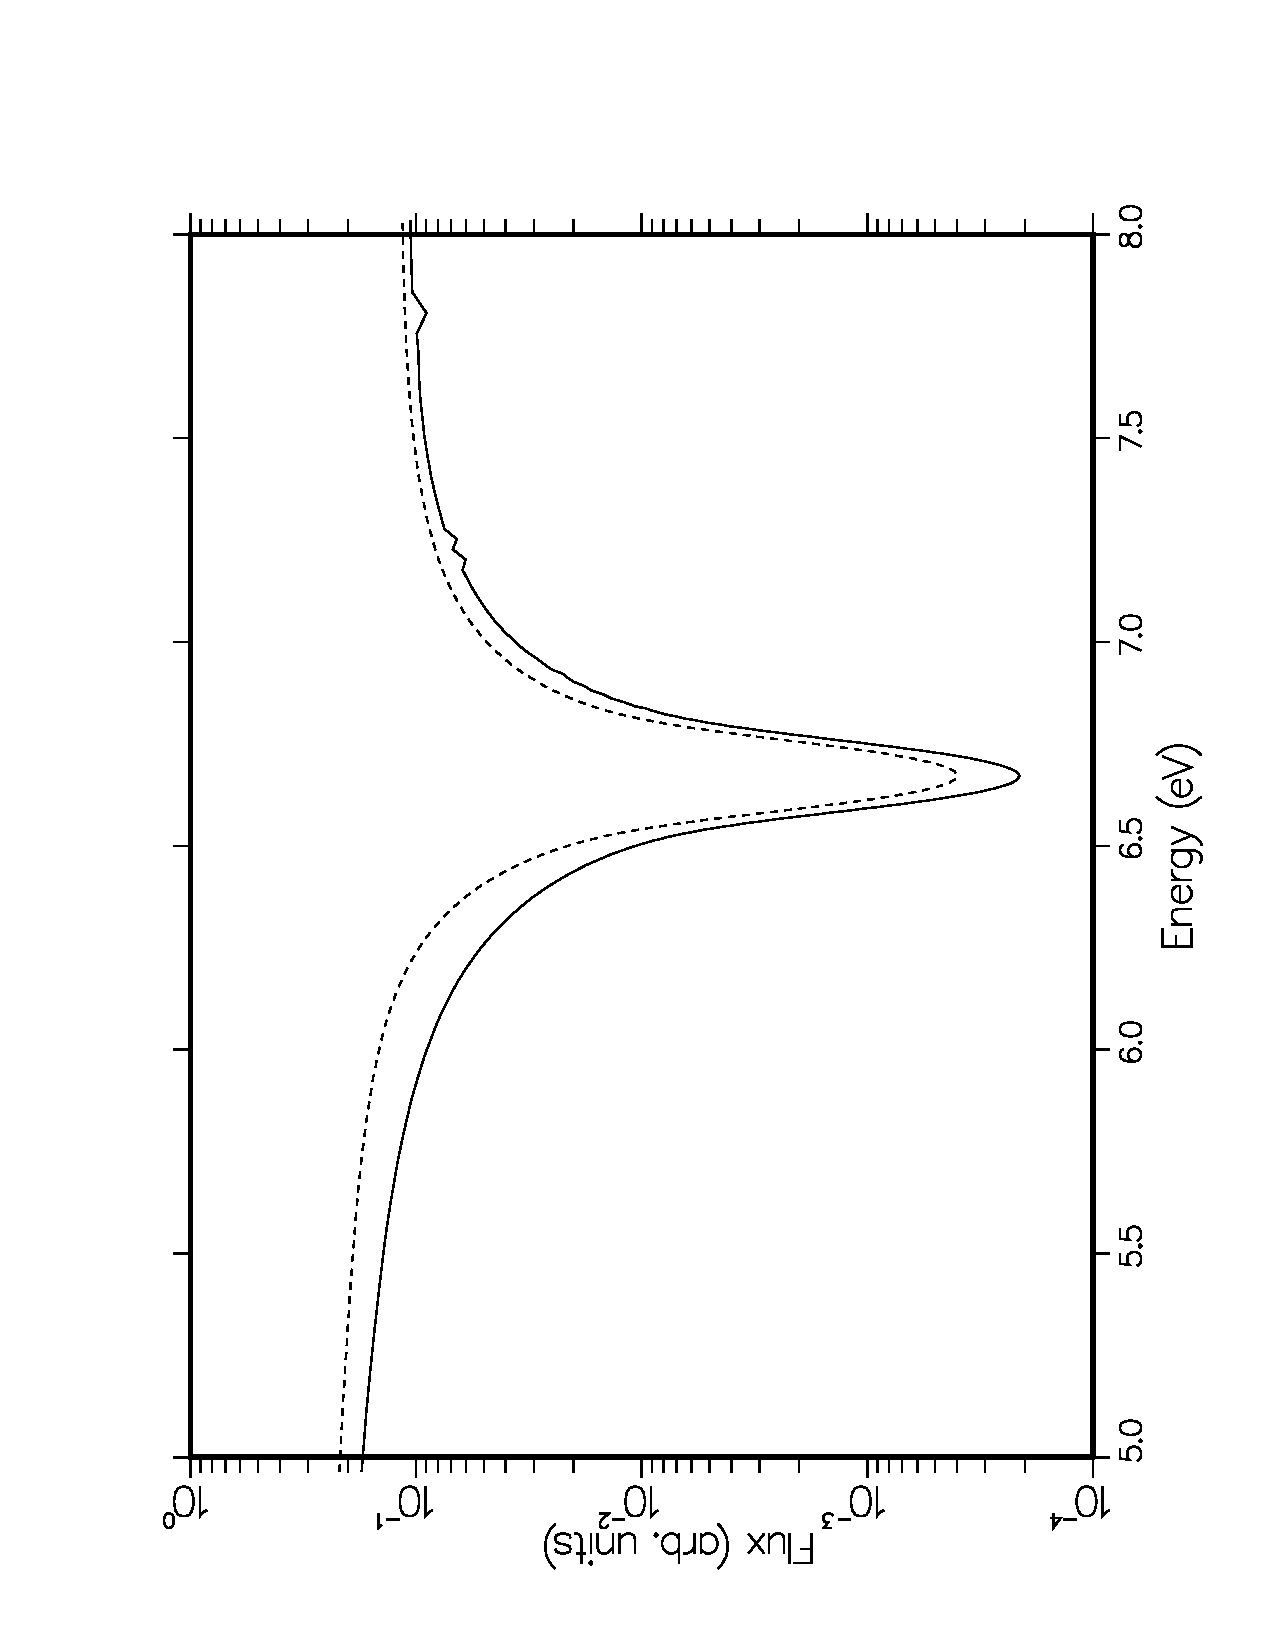
\includegraphics[keepaspectratio, height=3.5in, angle=270]{figs/groupr2ack}
\caption[Flux model predictions for $^{238}$UO$_2$ in water in the region
 near the 6.7 eV $^{238}$U resonance]{A comparison of the Bondarenko flux
 model (dashed) with a realistic computed flux (solid) for a $^{238}$U oxide
 pin in water in the region of the 6.7 eV resonance.}
\label{gr2}
\end{figure}

In practice, a fuel rod rarely contains only one resonance isotope.
\index{resonance interference}
As an example, consider a mixture of a few percent of $^{239}$Pu
with $^{238}$U as the major component.  There will be a strong dip in the
flux associated with the 6.7 eV $^{238}$U resonance that will affect the
flux in the region of the 7.8 eV $^{239}$Pu resonance (the interference
effect), and there will also be a dip in the flux corresponding to the
7.8 eV resonance (the self-shielding effect).  This additional
complication in the flux shape would be expected to change the group
constants for $^{239}$Pu since both features lie in the same group for
typical group structures.  However, the effect of the $^{239}$Pu on the
$^{238}$U group constants should be minimal.  This argument suggests that
the full flux calculation be used for $^{238}$U as a single resonance
material.  The resulting flux would then be used to estimate the flux
to be used in averaging the $^{239}$Pu cross sections as follows:

  \begin{equation}
    \phi_{239}(E,\sigma_0)={\displaystyle{\phi_{238}(E,50)}\over
    \displaystyle \sigma_0+{\displaystyle{\sigma_{239}(E)}\over\displaystyle
    {1+{\displaystyle{\sigma_{238}(E)\over\displaystyle 50}}}}}\,\,,
  \label{Eq38}
  \end{equation}
\vspace{0.5 pt}

\noindent
where the $^{238}$U flux is characteristic of a background of 50
barns/atom, which is representative of many thermal reactor systems.
This formula assumes that the effect of $^{239}$Pu on the scattering source
for the mixture is small, but it retains the absorption effects.  The
self-shielding of $^{239}$Pu is treated in the narrow resonance
approximation only.  The GROUPR flux calculator includes an option to
write out a file containing the calculated flux and cross section
needed for this formula ({\it e.g.}, for $^{238}$U) and another option
to skip the flux calculation and use the formula above to obtain the
weighting flux ({\it e.g.}, for $^{239}$Pu).

The slowing-down integral equation of Eq.~\ref{Eq33} or \ref{Eq37}
is solved point by point (see subroutine \cword{genflx}) using the
total and elastic cross sections on the PENDF tape produced by
\hyperlink{sRECONRhy}{RECONR}.
In order to keep this task within bounds, the flux is computed from the
lower limit of the first group to a specified energy \cword{fehi} or
until \cword{nfmax} values have been computed.  The flux at higher
energies is continued using the Bondarenko model described above.
\index{Bondarenko method}

\subsection{Fission Source}
\label{ssGROUPR_FissSource}

The fission source\index{fission source} was included in the
transfer cross section $\sigma_X$ in the development above.  It is
usually convenient to separate fission from scattering.  Assuming
isotropy, the source of fission neutrons into group $g$ is given by

  \begin{equation}
    S_g=\sum_{g'}\sigma_{fg'\rightarrow g}\,\phi_{0g'}\,\,,
  \end{equation}

\noindent
where the group-to-group matrix\index{fission matrix}
for fission is defined as in Eq.~\ref{Eq12}, but with $\ell$ equal
to zero.  Most existing transport codes do not use this matrix
form directly because the upscatter is expensive to handle and
a reasonably accurate alternative exists.  Except for relatively
high neutron energies, the spectrum of fission neutrons is only
weakly dependent on initial energy.  Therefore, the fission source
can be written

  \begin{equation}
    S_g=\chi_g\sum_{g'}\,\overline\nu_{g'}\,\sigma_{fg'}\,\phi_{0g'}\,\,,
  \end{equation}

\noindent
where $\overline\nu_g$ is the fission neutron yield, $\sigma_{fg}$ is the
fission cross section, and $\chi_g$ is the average fission spectrum
(the familiar ``chi'' vector\index{fission chi}), which can be defined by

  \begin{equation}
    \chi_g={\displaystyle{\sum_{g'}\sigma_{fg'\rightarrow g}\,\phi_{0g'}}
    \over\displaystyle{\sum_{g}\sum_{g'}\sigma_{fg'\rightarrow g}
    \,\phi_{0g'}}}\,\,.
  \label{Eq41}
  \end{equation}

\noindent
The fission neutron yield is given by
\index{fission neutron yield}

  \begin{equation}
    \overline\nu_{g}
    = \sum_{g'}\sigma_{fg\rightarrow g'}\,/\,\sigma_{fg}\,\,.
  \end{equation}

\noindent
Clearly, $\chi_g$ as given by Eq.~\ref{Eq41} depends on the flux in the
system of interest.  The dependence is weak except for high incident
energies, and a rough guess for $\phi_{0g}$ usually gives an accurate
spectrum.  When this is not the case, the problem can be iterated, or
the full matrix representation can be used.

It is possible to take advantage of the weak energy dependence of the
shape of the fission spectrum at low energies to reduce the time required
to process fission data, and to reduce the size of the fission data on the
output file.  GROUPR determines a break energy from File 5 such that
the fission spectrum is constant below this energy.  It only has to make
a single calculation of this spectrum $\chi^{LE}_g$.  Then it computes
a fission neutron production cross section $\sigma^{HE}_{fPg}$ for
groups below the break energy using the normal cross section processing
methods.  A full matrix $\sigma^{HE}_{fg'{\rightarrow}g}$ is computed
for groups above the break point.  As an example, consider using the
GROUPR 187-group structure and finding that there are 130 constant groups.
The 187${\times}$187 matrix is reduced to a 57${\times}$187 matrix,
a 187-element spectrum vector, and a 130-group production vector, for
a total reduction in size of 68\%.  The effective fission matrix is
given by

\begin{equation}
   \sigma_{fg'{\rightarrow}g}=\sigma^{HE}_{fg'{\rightarrow}g}
      + \chi^{LE}_g\sigma^{LE}_{fPg'} \,\,.
\end{equation}
\vspace{0.5 pt}

The fission matrix computed by GROUPR represents the prompt part
of fission only\index{prompt fission}.  The delayed component of
fission is represented\index{delayed fission} by a delayed-neutron
yield $\overline\nu_{g}^D$, decay constants for six (or sometimes 8)
time groups, $\lambda_i^D$, and emission probability spectra for
six (or 8) time groups, $\chi_{ig}^D$.  Steady-state fission
\index{fission, steady-state} can be obtained using

  \begin{equation}
    \overline\nu_g^{SS}=\overline\nu_g
    +\overline\nu_g^D\,\,,
  \end{equation}

\noindent
and

  \begin{equation}
    \chi_g^{SS}={\displaystyle{\sum_{g'}\sigma_{fg'\rightarrow g}\,\phi_{0g'}
    +\chi_g^D\sum_{g'}\overline\nu_{g'}^D\,\sigma_{fg'}\,\phi_{0g'}}
    \over\displaystyle{\sum_g\sum_{g'}\sigma_{fg'\rightarrow g}\,\phi_{0g'}
    +\sum_{g'}\overline\nu_{g'}^D\,\sigma_{fg'}\,\phi_{0g'}}}\,\,,
  \end{equation}

\noindent
where

  \begin{equation}
    \chi_g^D=\sum_i\chi_{ig}^D\,\,.
  \end{equation}

\noindent
Note that $\chi_g^D$ sums to unity, but the $\chi$ for each time group
sums to the fraction of the delayed neutron yield that appears
in that time group.
\index{delayed chi}
\index{delayed-neutron yield}

In ENDF-format files, the total fission reaction is represented
by MT=18.  Important isotopes also give the partial fission reactions
\index{partial fission} (n,f), (n,n$'$f), (n,2nf), and sometimes (n,3nf)
using MT=19, 20, 21, and 38 respectively.  The MT=18 representation is
adequate for most fission reactor applications, but the partial reactions
should be processed for applications with significant flux above 6 MeV.
Caution:  although the cross section for MT=18 equals the sum of its
parts, the group-to-group fission matrix $\sigma_{fg\rightarrow g'}$
computed from MT=18 will not, in general, equal the sum of the
partial matrices for MT=19, 20, 21, and 38 above the 6-MeV threshold
for second-chance fission.  The breakup into partial fission matrices
has not been used in recent ENDF/B-VII evaluations.  The
delayed neutron data are given in MT=455.  Sample input instructions
for processing the various combinations of fission reactions used
in ENDF/B will be found in Section~\ref{ssGROUPR_Continuum}.  GROUPR outputs all
the components of fission separately in order to give succeeding
modules or codes complete flexibility.

\subsection{Diffusion Cross Sections}
\label{ssGROUPR_Diffusion}

The diffusion equation is often used in reactor physics
calculations.\index{diffusion constant}  Starting with
Eq.~\ref{Eq7}, use the Legendre expansion
for $\phi_g$ in the derivative term, and make use of the recursion
relation for $\mu P_{\ell}(\mu)$ and the orthogonality relation for
the Legendre polynomials to obtain the transport equation in
spherical-harmonic form

  \begin{eqnarray}
    {{n+1}\over{2n+1}}{{\partial\phi_{n+1,g}}\over{\partial x}}
    &+&{{n}\over{2n+1}}{{\partial\phi_{n-1,g}}\over{\partial x}}
    \,\sigma_{tng}\,\phi_{ng}\nonumber\\
    \mbox{ }\nonumber\\
    &=& \sum_{g'}\sigma_{sng'\rightarrow g}\,\phi_{ng'}+S_{fg}+Q_{ng}\,\,,
  \end{eqnarray}

\noindent
where the transfer term has been separated into a scattering term with
cross section $\sigma_s$, and a fission source term $S_f$.  When this set
of equations is truncated at $n={\rm N} $, the results are usually called
the ``P$_{\rm N}$ equations''.  For now, all terms with $n>1$ are dropped,
and $Q$ is assumed to be isotropic.  Thus,

  \begin{equation}
    {{\partial\phi_{1g}}\over{\partial x}}
    +\sigma_{t0g}\,\phi_{0g}
    =\sum_{g'}\sigma_{s0g'\rightarrow g}\,\phi_{0g'}
    +S_{fg}+Q_{0g}\,\,,
  \label{Eq47}
  \end{equation}

\noindent
and

  \begin{equation}
    {1\over 3}{{\partial\phi_{0g}}\over{\partial x}}
    +\sigma_{t1g}\,\phi_{1g}
    =\sum_{g'}\sigma_{s1g'\rightarrow g}\,\phi_{1g'}\,\,.
  \end{equation}

\noindent
The second equation can be written in the form of Fick's Law as follows:

  \begin{equation}
    \phi_{1g}=-D_g{{\partial\phi_{0g}}\over{\partial x}}\,\,,
  \end{equation}

  \begin{equation}
    D_g={1\over 3}\,{1\over\displaystyle{
    \sigma_{t1g}-{\displaystyle{\sum_{g'}\sigma_{s1g'\rightarrow g}
    \,\phi_{1g'}}\, / \,\displaystyle{\phi_{1g}}}}}\,\,,
  \label{Eq50}
  \end{equation}

\noindent
where $D_g$ is the diffusion constant.  The term in the denominator of
the second factor is the transport cross section for diffusion,
$\sigma_{trD}$.  Unfortunately, it depends on a fairly complete knowledge
of the neutron current in the system, perhaps from a previous calculation.
However, for many problems, $\sigma_{trD}$ can be simplified by assuming that

  \begin{equation}
    \sum_{g'}\sigma_{s1g'\rightarrow g}\,\phi_{1g'}\approx
    \sum_{g'}\sigma_{s1g\rightarrow g'}\,\phi_{1g}\,\,,
  \end{equation}

\noindent
with the result that

  \begin{equation}
    \sigma_{trD,g}=\sigma_{t1g}-\sum_{g'}\sigma_{s1g\rightarrow g'}\,\,,
  \label{Eq52}
  \end{equation}

\noindent
or

  \begin{equation}
    \sigma_{trD,g}=\sigma_{t1g}-\overline\mu_g\,\sigma_{s0g}\,\,,
  \end{equation}

\noindent
where $\overline\mu_g$ is the average scattering cosine for neutrons
in group $g$.  These forms depend only on the shape of the weighting
flux within the group, as usual.  Substituting for $\phi_{1g}$ in
Eq.~\ref{Eq47} gives

  \begin{equation}
    {{\partial}\over{\partial x}}\bigl(-D_g
    {{\partial\phi_{0g}}\over{\partial x}}\bigr)
    +\sigma_{0tg}\,\phi_{0g}
    =\sum_{g'}\sigma_{s0g'\rightarrow g}\,\phi_{0g'}
    +S_{fg}+Q_{0g}\,\,,
  \end{equation}

\noindent
which is the standard diffusion equation in slab geometry.  Neither the
diffusion coefficient nor the transport cross section for diffusion is
produced directly by GROUPR.  However, the components such a
$\sigma_{t\ell}$ and $\sigma_{s0g'\rightarrow g}$ are made available
to subsequent modules.

\subsection{Cross Sections for Transport Theory}
\label{ssGROUPR_Transport}

The S$_{\rm N}$ (discrete ordinates) transport codes solve the equation
\index{discrete-ordinates transport}
\index{S$_{\rm N}$ transport}

  \begin{eqnarray}
    \mu{{\partial}\over{\partial x}}\phi_g(\mu,x)
    &+&\sigma_g^{SN}\phi_g(\mu,x)\nonumber\\
    &=&\sum_{\ell=0}^N{{2\ell+1}\over{2}}P_{\ell}(\mu)
    \sum_{g'}\sigma_{s\ell g'\rightarrow g}^{SN}(x)\,\phi_{\ell g'}
    \nonumber\\
    &+&S_{fg}+Q_g(\mu,x)\,\,,
  \label{Eq55}
  \end{eqnarray}

\noindent
where once again one-dimensional slab geometry has been used for
simplicity.\footnote{The following development is based on the work of
Bell, Hansen, and Sandmeier\cite{ref10}.} By comparing Eq.~\ref{Eq55}
with Eq.~\ref{Eq7}, it is seen that the S$_{\rm N}$ equations require
the following cross sections:

  \begin{equation}
    \sigma_{s\ell g'\rightarrow g}^{SN}=\sigma_{s\ell g'\rightarrow g}
    ,\qquad g'\ne g\,\,,
  \end{equation}

\noindent
and

  \begin{equation}
    \sigma_{s\ell g\rightarrow g}^{SN}=\sigma_{s\ell g\rightarrow g}
    -\sigma_{t\ell g}+\sigma_g^{SN}\,\,,
  \end{equation}

\noindent
where $\sigma_g^{SN}$ is not determined and can be chosen to improve
the convergence of the S$_N$ calculation.  A particular choice of
$\sigma_g^{SN}$ gives rise to a ``transport approximation'',
\index{transport approximations}
and various recipes are in use, such as:

Consistent-P approximation:

  \begin{equation}
    \sigma_g^{SN}=\sigma_{t0g}\,\,.
  \end{equation}

Inconsistent-P approximation:

  \begin{equation}
    \sigma_g^{SN}=\sigma_{t,N+1,g}\,\,.
  \end{equation}

Diagonal transport approximation:

  \begin{equation}
    \sigma_g^{SN}=\sigma_{t,N+1,g}-\sigma_{s,N+1,g\rightarrow g}\,\,.
  \end{equation}

Bell-Hansen-Sandmeier (BHS) or extended transport approximation:

  \begin{equation}
    \sigma_g^{SN}=\sigma_{t,N+1,g}-\sum_{g'}\sigma_{s,N+1,g\rightarrow g'}\,\,.
  \end{equation}

Inflow transport approximation:

  \begin{equation}
    \sigma_g^{SN}=\sigma_{t,N+1,g}-{\displaystyle
    {\sum_{g'}\sigma_{s,N+1,g'\rightarrow g}\,\phi_{N+1,g'}}
    \over\displaystyle{\phi_{N+1,g}}}\,\,.
  \end{equation}

\noindent
The first two approximations are most appropriate when the scattering orders
above N are small.  The inconsistent option removes most of the delta
function of forward scattering introduced by the correction for the
anisotropy of the total scattering rate, and should normally be more
convergent than the consistent option.  The diagonal and BHS recipes
make an attempt to correct for anisotropy in the scattering matrix and
are especially effective for forward-peaked scattering.  The BHS form
is more often used, but the diagonal option can be substituted when BHS
produces negative values.  The inflow recipe makes the $N{+}1$ term of
the P$_{\rm N}$ expansion vanish, but it requires a good knowledge of
the $N{+}1$ flux moment from some previous calculation.  Inflow reduces
to BHS for systems in equilibrium by detail balance ({\it i.e.}, the
thermal region).  In the absence of self-shielding (that is,
$\sigma_0{\rightarrow}\infty$), the distinction between $\sigma_{t1}$
and $\sigma_{t0}$ disappears, and so does the distinction between the
inconsistent-P and consistent-P options.  Also note that the inflow
and BHS versions of $\sigma_g$ are equivalent to the definitions of
$\sigma_{trD,g}$ given in Eqs.~\ref{Eq50} and \ref{Eq52}, respectively,
when $N{=}0$.

The transport-corrected cross sections are not computed directly
by GROUPR, but the components needed are written to the GROUPR output
file for use by subsequent modules.

\subsection{Photon Production and Coupled Sets}
\label{ssGROUPR_CoupledPhoton}

Photon transport\index{photon transport}
is treated with an equation similar to Eq.~\ref{Eq7},
except that the flux, cross sections, and groups are all referred to
photon interactions and photon energies instead of to the corresponding
neutron quantities.  Methods of producing the photon interaction cross
sections are described in
\hyperlink{sGAMINRhy}{GAMINR}.
\index{photon interaction cross sections}  The
external photon source $Q_g$ depends on the neutron flux and the
photon production cross sections through

  \begin{equation}
    Q_g(x,\mu)=\sum_{\ell=0}^{\infty}{{2\ell+1}\over{2}}
    P_{\ell}(\mu)\sum_{g'}\sigma_{\gamma\ell g'\rightarrow g}(x)
    \,\phi_{\ell g'}(x)\,\,,
  \end{equation}
\vspace{1 pt}

\noindent
where $\sigma_{\gamma\ell g'\rightarrow g}$ is defined by
Eq.~\ref{Eq12} with X replaced by $\gamma$.  The ENDF files define
$\sigma_{\gamma}$ using a combination of photon production cross sections
(MF=13), photon yields (MF=12) with respect to neutron cross sections
(MF=3), discrete lines (MF=12 and 13), and continuous $\gamma$
distributions (MF=15).  Methods for working with these representations
will be discussed in more detail below.

The low-energy groups for fission and capture normally have photon
emission spectra whose shapes do not change with energy.  The same
method used for reducing the size of the fission matrix (see
Section~\ref{ssGROUPR_FissSource}) can be used for these photon production
matrices.  In mathematical form,

\begin{equation}
   \sigma_{\gamma g'{\rightarrow}g}=\sigma^{HE}_{\gamma g'{\rightarrow}g}
      + s^{LE}_\gamma g\sigma^{LE}_{\gamma Pg'} \,\,,
\end{equation}
\vspace{1 pt}

\noindent
where $s^{LE}_\gamma g$ is the normalized emission spectrum, and
$\sigma^{LE}_{\gamma Pg}$ is the associated production cross section.

For many practical problems, it is convenient to combine the neutron
and photon transport calculations into a single application of
Eq.~\ref{Eq7} where the photons are treated as additional groups of
low-energy neutrons.  Since ($\gamma$,n) events are not usually very
important, the downscattering structure
(see Section~\ref{ssGROUPR_Group_Order}) of the
transport calculation is preserved for both n${\rightarrow}\gamma$ and
n$\rightarrow$n events.  Cross sections for this application are called
``coupled sets''.  Coupled sets\index{coupled sets} are not produced
directly by GROUPR, but the n$\rightarrow$n and n${\rightarrow}\gamma$
components are made available to the other modules where they can be
combined with $\gamma{\rightarrow}\gamma$ cross sections from
\hyperlink{sGAMINRhy}{GAMINR}\index{GAMINR}.  As an example, the
\hyperlink{sMATXSRhy}{MATXSR}\index{MATXSR} module
can format data for the TRANSX code,\index{TRANSX} which can, in turn,
prepare coupled sets for use by standard transport codes such as
ONEDANT\cite{ONEDANT} or PARTISN\cite{PARTISN}.  The normal
arrangement of data in a coupled set is shown schematically
in Fig.~\ref{gr3}.

\begin{figure}[b]\centering
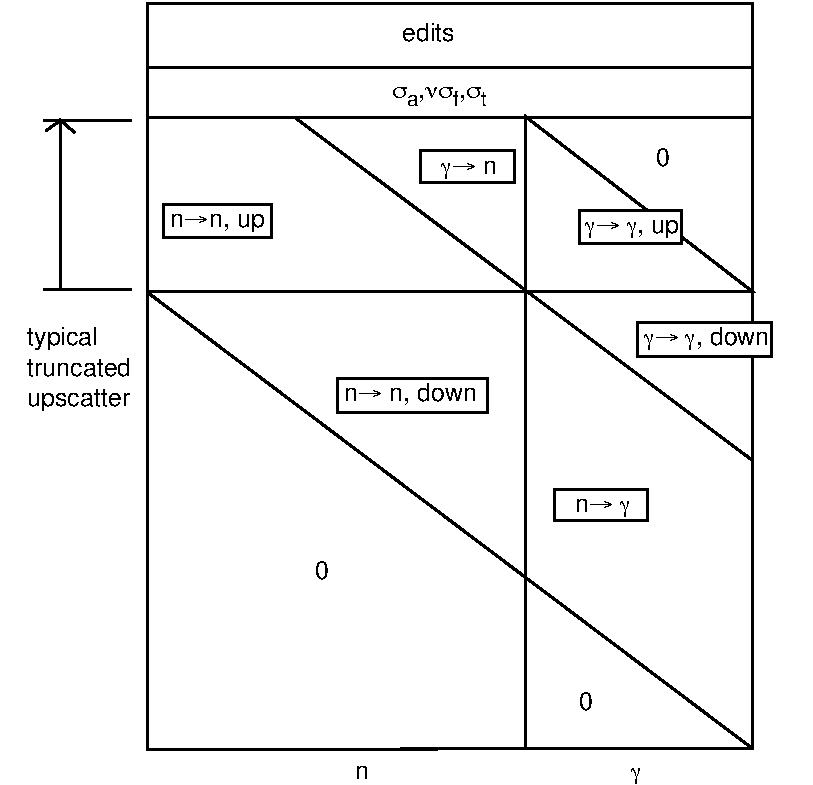
\includegraphics[keepaspectratio, height=4.6in, angle=0]{figs/groupr3}
\caption[Coupled Neutron/Photon Tables]{Arrangement of neutron (n) and
 photon ($\gamma$) cross sections in a coupled transport table.  The group
 index increases from left to right, and the position index increases from top
 to bottom.  The $\gamma{\rightarrow}$n and $\gamma{\rightarrow}\gamma$
 upscatter blocks are normally empty.}
\label{gr3}
\end{figure}

\subsection{Thermal Data}
\label{ssGROUPR_Thermal}

GROUPR uses the thermal data written onto the PENDF tape
by the \hyperlink{sTHERMRhy}{THERMR} module\index{THERMR}.  It
does not process ENDF File-7\index{File 7}
data directly.  Three different representations of thermal scattering
are used in ENDF.

For crystalline materials like graphite, coherent elastic (with zero
energy change)\index{coherent elastic} scattering can take place.  The
cross section for this process shows well-defined Bragg
edges\index{Bragg edges} at energies that correspond to the
various lattice-plane spacings in the crystalline powder.  As shown
in \hyperlink{sTHERMRhy}{THERMR},\index{THERMR} the angular dependence of the
coherent elastic cross section can be written as

  \begin{equation}
    \sigma^{coh}(E,\mu)=\sum_i {{b_i} \over {E}}
    \,\delta(\mu-\mu_i)\,\,,
  \label{Eq64}
  \end{equation}

\noindent
where

  \begin{equation}
    \mu_i=1-2{{E_i} \over {E}}\,\,,
  \end{equation}

\noindent
and where the $E_i$ are the energies of the Bragg
edges.  \hyperlink{sTHERMRhy}{THERMR}
integrates Eq.~\ref{Eq64} over all angles, and writes the result
to the PENDF tape.  Clearly, the $b_i$ can be recovered from

  \begin{equation}
    E\,\sigma^{coh}(E)=\mathop{{\sum}'}_i b_i\,\,,
  \label{Eq66}
  \end{equation}
\vspace{1 pt}

\noindent
where the primed sum is over all $i$ such that $E_i <E$.  It is only
necessary to locate the steps in $E\,\sigma^{coh}(E)$.  The size of the
step gives $b_i$, and the $E$ for the step gives $E_i$.  The Legendre
cross sections become

  \begin{equation}
    \sigma^{coh}_\ell (E)=\mathop{{\sum}'}_i {{b_i} \over {E}}
     P_\ell (\mu_i)\,\,,
  \label{Eq67}
  \end{equation}

\noindent
where any terms with $\mu_i{<}-1$ are omitted from the primed sum.
An example of a pointwise cross section for coherent elastic scattering
is given in Fig.~\ref{gr4}.

\begin{figure}[thb]\centering
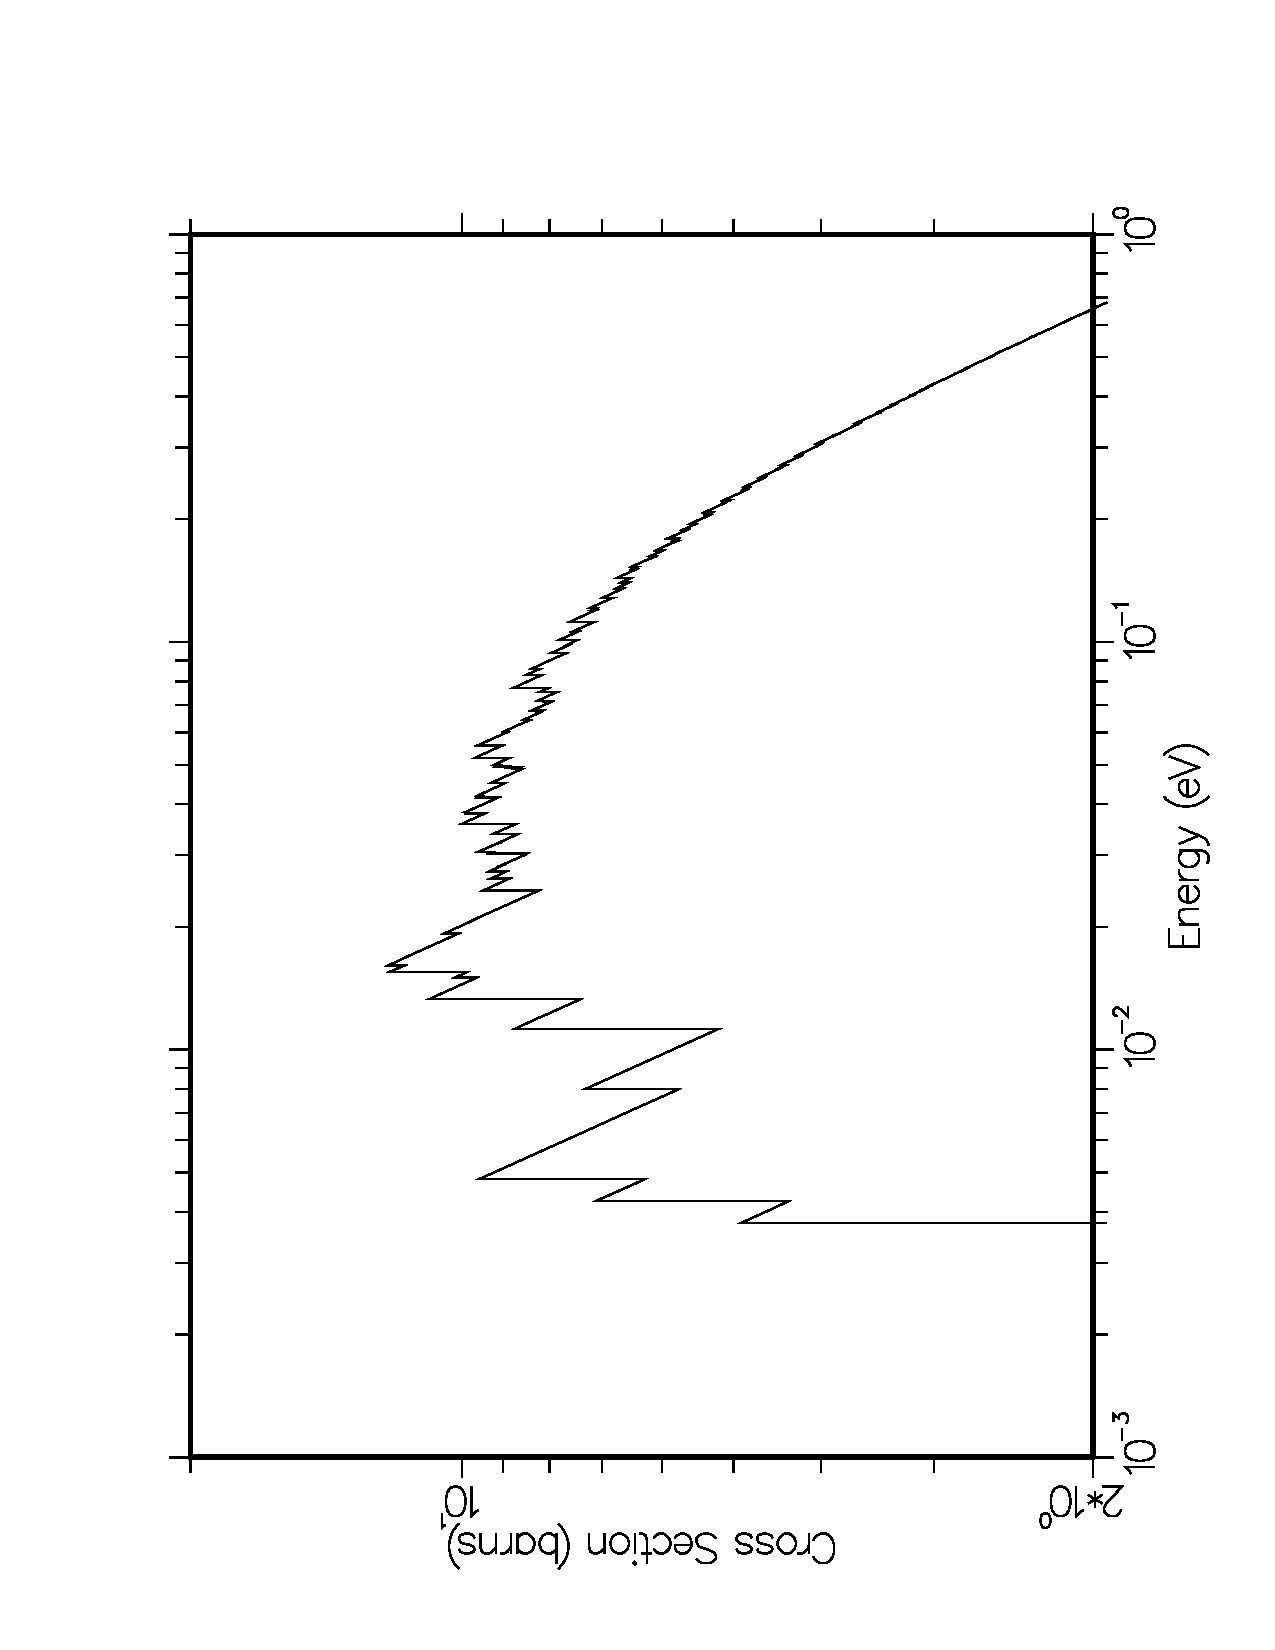
\includegraphics[keepaspectratio, height=3.5in, angle=270]{figs/groupr4ack}
\caption[Bragg edges seen in the BeO coherent elastic scattering cross section]
{The coherent elastic scattering cross section for BeO showing the Bragg edges.
 The shape of $\sigma(E)$ between edges is $1/E$.  Therefore, the function
 $E\sigma(E)$ is a stair-step function, where the height of each step depends
 on the structure factor for
 scattering from that set of lattice planes (see Eq.~\ref{Eq66}).}
\label{gr4}
\end{figure}

For hydrogenous solids like polyethylene and zirconium hydride, the
process of incoherent elastic scattering\index{incoherent elastic}
is important.  Here the angular cross section is given by

  \begin{equation}
    \sigma^{iel}(E,\mu)={{\sigma_b}\over 2}
    \exp \biggl[ -{{2EW}\over A} (1-\mu) \biggr]\,\,.
  \end{equation}
\vspace{0.5 pt}

\noindent
\hyperlink{sTHERMRhy}{THERMR} converts this into
an integrated cross section, $\sigma^{iel}(E)$, and a set of $N$
equally probable emission cosines, $\overline{\mu}_i$.  These angles
are present in File 6 on the PENDF tape.  GROUPR can easily determine
the Legendre components of the scattering cross section using

  \begin{equation}
    \sigma^{iel}_{\ell} (E)=\sigma^{iel}(E)
    {{1}\over {N}} \sum_{i=1}^N P_{\ell} (\mu_i )\,\,.
  \label{Eq69}
  \end{equation}

The third thermal process is incoherent inelastic scattering.
\index{incoherent inelastic} Here the neutron energy can either
increase or decrease.  The data from
\hyperlink{sTHERMRhy}{THERMR} are given as a
cross section in File 3 and an energy-angle distribution
using a special form of File 6.  The distribution is
represented by sets of secondary-energy values $E'$ for particular
incident energies $E$.  For each $E{\rightarrow}E'$, a scattering
probability $f^{inc} (E{\rightarrow}E')$ and a set of equally probable
cosines $\mu_i (E{\rightarrow}E')$ are given.  The scattering probabilities
for each value of $E$ integrate to unity.  Although the thermal
scattering cross section is a smooth function of incident neutron energy,
this is not true for the scattering from $E$ to one particular final
energy group $g'$, since the differential cross section tends to peak
along the line $E'{=}E$ and at energy-transfer values corresponding
to well-defined excitations in the molecule or lattice.  If interpolation
between adjacent values of $E$ were to be performed along lines of
constant $E'$, the excitation peaks and the $E{=}E'$ feature would
produce double features in the intermediate spectrum, as shown in
Fig.~\ref{gr5}.  To avoid this problem, while still using a
relatively sparse incident energy grid, GROUPR interpolates between
$E$ and $E'$ along lines of constant energy transfer.  Of course, this
breaks down at low values of $E'$, because one of the spectra will go
to zero before the other one does.  In this range, GROUPR transforms
the low-energy parts of the two spectra onto a ``unit base,'' combines
them in fractions that depend on $E$, and scales the result back out
to the interpolated value of $E'$ corresponding to $E$.

\begin{figure}[tp]\centering
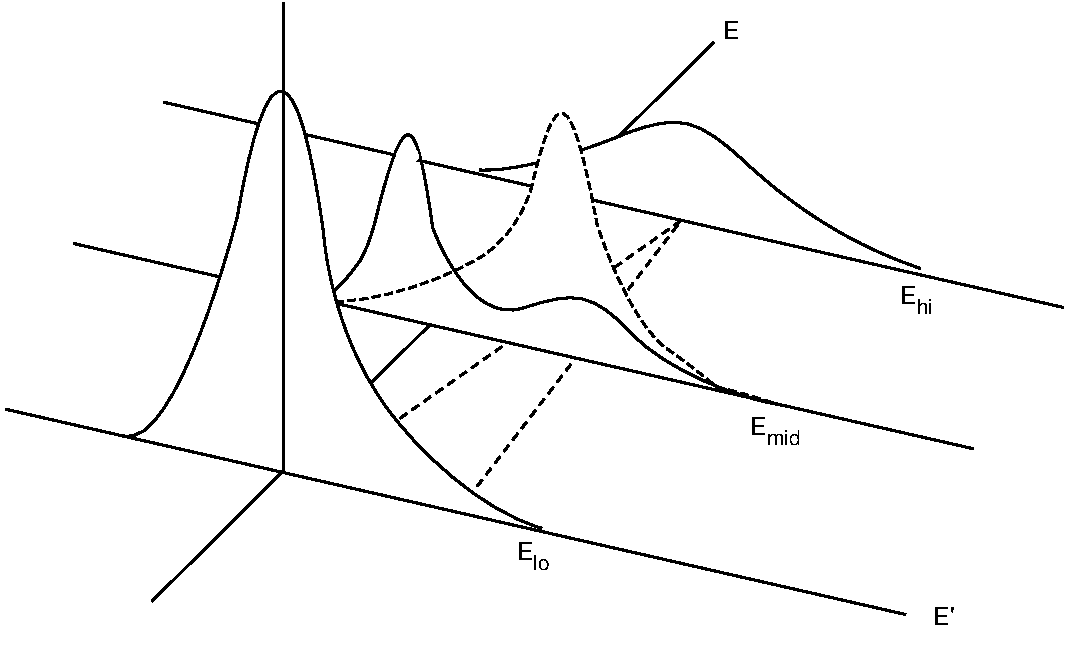
\includegraphics[keepaspectratio, height=3.25in, angle=0]{figs/groupr5}
\caption[Interpolation along lines of constant energy transfer]{Illustration of
 thermal interpolation showing the double-humped curve resulting from simple
 Cartesian interpolation for a discrete excitation (solid) and the more
 realistic curve obtained by interpolating along lines of constant energy
 transfer (dashed).}
\label{gr5}
\end{figure}

\subsection{Generalized Group Integrals}
\label{ssGROUPR_GrpInt}

In order to unify many formerly different processing tasks, GROUPR uses
the concept of a generalized group integral
  \begin{equation}
    \sigma_g={\displaystyle{\int_g {\cal F}(E)\,\sigma(E)\,\phi(E)\,dE}
    \over\displaystyle{\int_g\phi(E)\,dE}}\,\,,
  \label{Eq70}
  \end{equation}
where the integrals are over all initial neutron energies in group $g$,
$\sigma(E)$ is a cross section at $E$, and $\phi(E)$ is an estimate of
the flux at $E$.  The function ${\cal F}(E)$ is called the ``feed function''.
\index{feed function}
It alone changes for different data types.  To average a neutron cross
section, ${\cal F}$ is set to 1.  To average a ratio quantity like
$\overline \mu$ with respect to elastic scattering, ${\cal F}$ is set
to $\overline \mu$.  For photon production, ${\cal F}$ is the photon yield.
For matrices, ${\cal F}$ is the  $\ell$-th Legendre component of
the normalized probability of scattering into secondary energy group
$g'$ from initial energy $E$.  This definition is clearly independent of
whether the secondary particle is a neutron or a photon.

The question of integration grid or quadrature scheme is important for
the evaluation of Eq.~\ref{Eq70}.  Each factor in the integrands has its
own characteristic features, and it is important to account for them all.
First, a grid must be established for each factor.  As an example, the
grid of $\sigma(E)$ is generated in
\hyperlink{sRECONRhy}{RECONR}\index{RECONR} such
that sigma can be obtained to within a given tolerance by
linear interpolation.  GROUPR contains a subroutine
\cword{getsig}\index{getsig@{\ty getsig}} which carries out this
interpolation at $E$ and also returns the next grid energy in
\cword{enext}.  Subroutines \cword{getflx}\index{getflx@{\ty getflx}}
and \cword{getff}\index{getff@{\ty getff}} perform similar functions
for the flux and feed function.  It is now easy to generate a
union grid for the three-factor integrand using the following Fortran:

\small
\begin{ccode}
       ...
      call getsig(e,enext,...)
      call getflx(e,en,...)
      if (en.lt.enext) enext=en
      call getff(e,en,...)
      if (en.lt.enext) enext=en
       ...
\end{ccode}
\normalsize

\noindent
On occasion, there will be a discontinuity at \cword{enext} for one of the
factors.  In order to flag such a case, each ``\cword{get}'' routine
also sets a discontinuity flag \cword{idisc}.  The grid logic actually
used throughout NJOY is as follows:

\small
\begin{ccode}
     ...
      call getsig(e,enext,idisc,...)
      call getflx(e,en,idis,...)
      if (en.eq.enext.and.idis.gt.idisc) idisc=idis
      if (en.lt.enext) idisc=idis
      if (en.lt.enext) enext=en
      call getff(e,en,idis,...)
      if (en.eq.enext.and.idis.gt.idisc) idisc=idis
      if (en.lt.enext) idisc=idis
      if (en.lt.enext) enext=en
      ...
\end{ccode}
\normalsize

\noindent
This union grid for the integrand in the numerator is used to subdivide
the generalized group integral of Eq.~\ref{Eq70} into ``panels''.  The
main program of GROUPR carries out the integrals with the following logic:

\small
\begin{ccode}
      ...
      elo=egn(ig)
      ehi=egn(ig+1)
      enext=ehi
  230 call panel(elo,enext,...)
      if (enext.eq.ehi) go to 240
      elo=enext
      enext=ehi
      go to 230
  240 continue
      ...
\end{ccode}
\normalsize

\noindent
A panel is first defined by the energy bounds of group $g$.  Subroutine
\cword{panel} is called to sum in the contributions from this panel.
However, \cword{panel} discovers that the integrand has a grid point at
\cword{enext} less than \cword{ehi}.  It adds in the contributions for
the smaller panel \cword{elo} to \cword{enext} and returns.  GROUPR now
sees that \cword{enext} is less than \cword{ehi}, so it tries a new panel
from the top of the last panel (\cword{elo}=\cword{enext}) to \cword{ehi}.
This loop continues until a panel with \cword{ehi} as its upper bound
is summed in.  The integral for this group is then complete.

In this simple way, the algorithm accounts for the user's group
structure and for all structure in the integrand.  The method used for
establishing the \hyperlink{sRECONRhy}{RECONR} grid
makes this integration algorithm
equivalent to adaptive integration as used in MINX\cite{MINX}.
It has the great advantage that no ``stack'' of intermediate results
is carried along.  This single-pass feature of the quadrature scheme
allows many different integrals to be accumulated simultaneously
within reasonable storage limits.  In this way, GROUPR accumulates
cross sections for all values of $\sigma_0$ simultaneously.  Similarly,
group-to-group cross sections are computed for all secondary energy
groups and all Legendre orders simultaneously.

Any degree of complexity can be used for the integral over each subpanel.
Because $\sigma(E)$ has been linearized, \cword{panel} is based on
trapezoidal integration.  Both $\phi(E)$ and
$R(E)=\sigma(E){\times}\phi(E)$ are assumed to vary linearly across each
panel.  In some cases, the feed function is oscillatory over a certain
energy range (see Two-Body Scattering, Section~\ref{ssGROUPR_TwoBody}).
It is then convenient to integrate inside the panel using Lobatto
quadrature\cite{ref13}\index{Lobatto quadrature} (note the variable
\cword{nq} in \cword{panel}\index{panel@{\ty panel}}).  As discussed
in more detail later, this method can obtain accurate results
for an oscillatory function whose integral is small with respect to its
magnitude.  This behavior is characteristic of the higher Legendre
components of two-body scattering cross sections.

The generalized integration scheme discussed here is also used by
the \hyperlink{sGAMINRhy}{GAMINR}\index{GAMINR}
and \hyperlink{sERRORRhy}{ERRORR}\index{ERRORR} modules.

\subsection{Two-Body Scattering}
\label{ssGROUPR_TwoBody}

Elastic scattering (ENDF/B MT=2) and discrete inelastic neutron
scattering (with MT=51 -- 90) are both examples of two-body kinematics
\index{two-body kinematics} and are treated together by GROUPR.  Some
other cases that occur for charged particles or in
File 6\index{File 6} will be discussed later.  The
feed function required for the group-to-group matrix calculation
may be written

  \begin{equation}
    {\cal F}_{\ell g'}(E)=\int_{g'}dE'\,\int_{-1}^{+1}d\omega\,
    f(E{\rightarrow}E',\omega)\,P_{\ell}(\mu[\omega])\,\,,
  \label{Eq71}
  \end{equation}

\noindent
where $f(E{\rightarrow}E',\omega)$ is the probability of scattering
from $E$ to $E'$ through a center-of-mass cosine $\omega$ and $P_{\ell}$
is a Legendre polynomial for laboratory cosine $\mu$.  The laboratory
cosine corresponding to $\omega$ is given by

  \begin{equation}
    \mu={{1+R\omega}\over
    {\sqrt{1+R^2+2R\omega }}}\,\,,
  \label{Eq72}
  \end{equation}

\noindent
and the cosine $\omega$ is related to secondary energy $E'$ by

  \begin{equation}
    \omega={{E'(1+A)^2/A'-E(1+R^2)}
    \over{2RE}}\,\,,
  \label{Eq73}
  \end{equation}

\noindent
where $A'$ is the ratio of the emitted particle mass to the incident
particle mass ($A'{=}1$ for neutron scattering).  In Eqs.~\ref{Eq72}
and \ref{Eq73}, $R$ is the effective mass ratio

  \begin{equation}
    R=\sqrt{\frac{A(A+1-A')}{A'}}\sqrt{1-{{(A+1)(-Q)}\over{AE}} }\,\,,
  \label{Eq74}
  \end{equation}

\noindent
where $A$ is the ratio of target mass to neutron mass, and $-Q$ is the
energy level of the excited nucleus ($Q{=}0$ for elastic scattering).
Integrating Eq.~\ref{Eq71} over secondary energy gives

  \begin{equation}
    {\cal F}_{\ell g'}(E)=\int_{\omega_1}^{\omega_2}
    f(E,\omega)\,P_{\ell}(\mu[\omega])\,d\omega\,\,,
  \label{Eq75}
  \end{equation}

\noindent
where $\omega_1$ and $\omega_2$ are evaluated using Eq.~\ref{Eq73}
for $E'$ equal to the upper and lower bounds of $g'$, respectively.
The scattering probability is given by

  \begin{equation}
    f(E,\omega)=\sum_{\ell=0}^L f_{\ell}(E)\,P_{\ell}(\omega)\,\,,
  \label{Eq76}
  \end{equation}

\noindent
where the Legendre coefficients are either retrieved directly from the
ENDF File 4 or computed from File 4 tabulated angular distributions
(see subroutines \cword{getfle}\index{getfle@{\ty getfle}} and
\cword{getco}\index{getco@{\ty getco}}).

The integration in Eq.~\ref{Eq75} is performed (see subroutine
\cword{getdis}\index{getdis@{\ty getdis}}) simultaneously for all
Legendre components using Gaussian quadrature\cite{ref13}.
\index{Gaussian quadrature}  The quadrature order is selected
based on the estimated polynomial order of the integrand.  A
reasonable estimate is given by

  \begin{equation}
    {\rm ND} + {\rm NL} +\log(300/A)\,\,,
  \label{Eq77}
  \end{equation}

\noindent
where ND is the number of Legendre components desired for the feed
function, and NL is the number of components required to represent
$f(E,\omega)$.  The log term approximates the number of additional
components required to represent the center-of-mass to lab transformation.

The two-body feed function for higher Legendre orders is a strongly
oscillatory function in some energy ranges.  An example is shown in
Fig.~\ref{gr6}.  Furthermore, the integral of the oscillatory part
is often small with respect to the magnitude of the function.  Such
functions are very difficult to integrate with adaptive techniques,
which converge to some fraction of the integral of the absolute value.
This is the reason that MINX\cite{MINX}\index{MINX} gave poor answers
for small Legendre components of the scattering matrix.  Gaussian methods,
on the other hand, are capable of integrating such oscillatory functions
exactly if they are polynomials.  Since a polynomial representation
of the feed function is fairly accurate, a Gaussian quadrature scheme
was chosen.  The scheme used is also well adapted to performing many
integrals in parallel.  In GROUPR, all Legendre components and all
final groups are accumulated simultaneously (see
\cword{panel}\index{panel@{\ty panel}}).

\begin{figure}[t]\centering
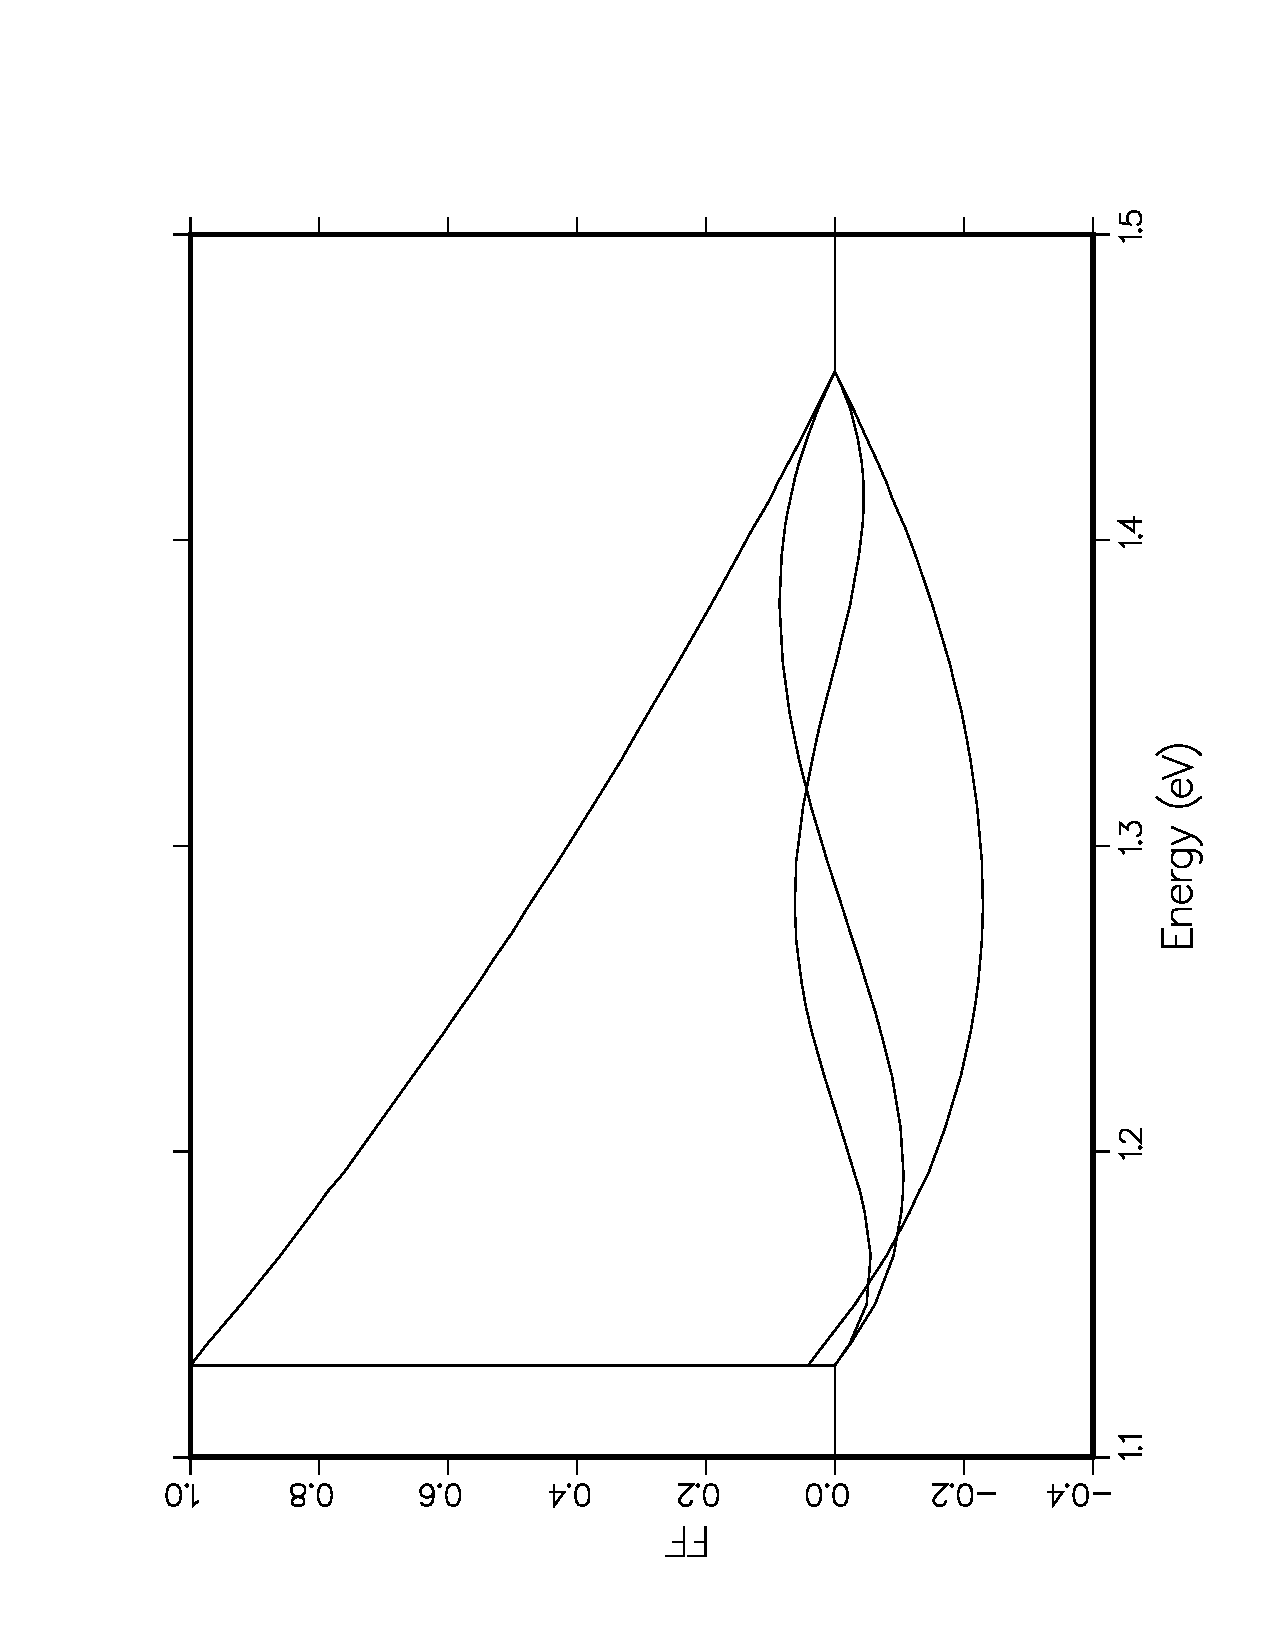
\includegraphics[keepaspectratio, height=3.5in, angle=-90]{figs/groupr6ack}
\caption[Sample two-body scattering feed function]{A typical feed
function for two-body scattering showing the oscillations that must
be treated correctly by the integration over incident energy.}
\label{gr6}
\end{figure}

The boundaries of the various regions of the feed function are
called ``critical points.''\index{critical points}  Between critical
points, the feed function is a smooth analytic function of
approximately known polynomial order.  It is only necessary
to add these critical points to the incident energy grid of
the feed function (the \cword{enext} variable) and to tell
\cword{panel}\index{panel@{\ty panel}} what quadrature order
(\cword{nq}) to use.  The critical points are determined in
\cword{getff}\index{getff@{\ty getff}} by solving Eq.~\ref{Eq73} for
the values of $E$ for which $\omega=+1$ and $\omega=-1$ when $E'$ is
equal to the various group boundaries.  This can be done by writing

  \begin{equation}
    {{E_g}\over{E}}=
    {{1}\over{(1+A)^2}}\bigl[ R^2\pm 2R+1\bigr]\,\,,
  \end{equation}
\vspace{0.5 pt}

\noindent
substituting for $E$ using Eq.~\ref{Eq74}, and then solving
for $R$.  The result is

  \begin{equation}
    E_{crit}={\displaystyle{ {{(A+1)(-Q)}\over{A}} }\over
    \displaystyle{1- {\displaystyle{A'F^2}\over{A(A+1-A')}} }}\,\,,
  \label{Eq79}
  \end{equation}
\vspace{0.5 pt}

\noindent
where
  \begin{equation}
    F={{1\pm\sqrt{D}}\over{1+ \displaystyle{{E_F}\over{(-Q)}} }}\,\,,
  \end{equation}
\vspace{0.5 pt}

  \begin{equation}
    D=\biggl[ \frac{A(A+1-A')}{A'}
       \biggl( 1+{{E_F}\over{(-Q)}} \biggr) -1 \biggr]
    {{E_F}\over{(-Q)}}\,\,,
  \end{equation}
\vspace{0.5 pt}

\noindent
and
  \begin{equation}
    E_F={{1+A}\over {A+1-A'}} E_g\,\,.
  \label{Eq82}
  \end{equation}

File 4 can also contain angular distributions for charged-particle
emission through discrete levels (for ENDF/B-VI and later see
MT=600 -- 648 for protons,
MT=650 -- 698 for deuterons, and so on; the elastic case, MT=2, is
discussed in the next section).  Moreover, File 6 can contain angular
distributions for discrete two-body scattering (see Law 3).  It can
also declare that a particular particle is the recoil particle
from a two-body reaction (Law 4), in which case the appropriate
angular distribution is obtained from the corresponding Law 3
subsection by complementing the angle.  The representation of the
angular distribution for these laws is almost identical to that
in File 4, and the calculation is done in
\cword{getdis}\index{getdis@{\ty getdis}} using much
of the File 4 coding.  The effects on the kinematics of the difference
in the mass of the emitted and incident particles are handled by the
variable $A'$ in the above equations.

\subsection{Charged-Particle Elastic Scattering}
\label{ssGROUPR_CPEl}

Coulomb scattering\index{Coulomb scattering} only occurs in the
elastic channel, and this calculation also uses the
\cword{getdis} subroutine.  The problem with Coulomb scattering
is that the basic Rutherford formula\index{Rutherford formula}
becomes singular at small angles.  In practice, this singularity
is removed by the screening effects of the atomic electrons.
\index{atomic screening}  The forward transport of charged
particles in this screening regime is usually handled by
continuous-slowing-down theory by using a ``stopping power''.
\index{stopping power}
The new ENDF-6 format allows for three different ways to handle the
large-angle scattering regime.  First and most general is the nuclear
amplitude expansion:\index{nuclear amplitude expansion}

\begin{eqnarray}
   \sigma&=&|{\rm nucl} + {\rm coul}|^2\nonumber\\
         &=& \sigma_{\rm nucl}+\sigma_{\rm coul}+{\rm interference}
\end{eqnarray}

\noindent
The Coulomb term is given by the Rutherford formula, a Legendre
expansion is defined for the nuclear term, and a complex Legendre
expansion is defined for the interference term.  This representation
cannot be generated directly from experimental data; an R-matrix
or phase-shift analysis is necessary.

A method very closely related to experiment ($\sigma_{\rm exp}$) is the
nuclear plus interference (NI) formula:
\index{nuclear plus interference}

\begin{equation}
   \sigma_{\rm NI}(\mu,E)=\sigma_{\rm exp}(\mu,E)
      -\sigma_{\rm coul}(\mu,E),
\end{equation}

\noindent
where the function is only defined for angles with cosines
$\mu{<}\mu_{\rm max}$.  The minimum angle is usually taken to be
somewhere around 20 degrees (GROUPR uses $\mu_{\rm max}{=}0.96$).
This function is still ill-behaved near the cutoff, and it must be
tabulated.  The third option is the residual cross section expansion:
\index{residual cross section expansion}

\begin{equation}
   \sigma_R(\mu,E)=(1-\mu)\bigl[\sigma_{\rm exp}(\mu,E)
      -\sigma_{\rm coul}(\mu,E)\bigr].
\end{equation}

\noindent
The $(1-\mu)$ term removes the pole at the origin.  The residual is
uncertain, but it is usually small enough that the entire curve can be
fitted with Legendre polynomials without worrying about what happens at
small angles.   In practice, both the nuclear amplitude expansion and
the nuclear plus interference representation are converted to the
residual cross section representation in subroutine
\cword{conver}\index{conver@{\ty conver}}.  As a result,
\cword{getdis}\index{getdis@{\ty getdis}} only has to cope with
the one representation.


\subsection{Continuum Scattering and Fission}
\label{ssGROUPR_Continuum}

In ENDF evaluations, scattering from many closely-spaced levels or
multibody scattering such as (n,2n), (n,n$'\alpha$) or fission is often
represented using a separable function of scattering cosine and
secondary neutron energy

  \begin{equation}
    f(E{\rightarrow}E',\mu)=F(E,\mu)\,g(E{\rightarrow}E')\,\,,
  \label{Eq83}
  \end{equation}

\noindent
where $F$ is the probability that a neutron will scatter through a
laboratory angle with cosine $\mu$ irrespective of final energy $E'$.  It is
obtained from MF=4.  Similarly, $g$ is the probability that a neutron's
energy will change from $E$ to $E'$ irrespective of the scattering angle,
and it is given in MF=5.  Continuum reactions are mostly identified by
MT numbers of 6 -- 49 and 91.  Recently, previously unused MT numbers,
152 through 200, were assigned to additional continuum reactions
that are beginning to appear in specialized evaluated files that extend
beyond 20 MeV ({\it e.g.}, the International Reactor Dosimetry and Fusion
File).  Secondary-energy distributions, whether found in MF=5 or MF=6
are represented by ``Laws" as follows:

\begin{center}
\begin{tabular}{cl}
Law & Description \\ \hline
1  & Arbitrary tabulated function \\
5  & General evaporation spectrum \\
   & (Used for delayed neutrons only.) \\
7  & Simple Maxwellian fission spectrum \\
9  & Evaporation spectrum \\
11 & Energy-dependent Watt fission spectrum \\
12 & Energy-dependent spectrum of Madland and Nix \\ \hline
\end{tabular}
\end{center}
\vspace{3 pt}

The feed functions for continuum scattering are simply

  \begin{equation}
    {\cal F}_{\ell g'}(E') = \int_{-1}^{+1} P_{\ell}(\mu) \,f(E,\mu)\,d\mu
    \int_{g'} g(E,E')\,dE'\,\,.
  \end{equation}
\vspace{0.5 pt}

\noindent
The first integral is returned by \cword{getfle} [``fle'' for $f_\ell (E)$]
as described above, and the second integral is returned by \cword{getsed}
(``sed'' for secondary-energy distribution).

For Law 1, $g$ is given as a tabulated function of $E'$ for various
values of E.  When $E_1\leq E<E_2$, the term $\int_{g'} g(E,E')\,dE'$ is
obtained by interpolating between precomputed values of
$\int_{g'} g(E_1,E')\,dE'$ and $\int_{g'} g(E_2,E')\,dE'$ in subroutine
\cword{getsed}.  Except in the case of fission, any apparent upscatter
produced by the ``stairstep'' treatment near $E{=}E'$ is added to the
in-group scattering term ($g'{=}g$).

For Law 5, $g(x)$ is given versus $x=E'/\theta(E)$ and $\theta(E)$
is given vs. E in File 5.  This secondary neutron distribution leads to
the following group integral:

  \begin{equation}
    \int_{g'}g(E,E')\,dE'=\theta(E)
    \int_{E_1/\theta}^{E_2/\theta}g(x)\,dx\,\,,
  \end{equation}
\vspace{0.5 pt}

\noindent
with $E_1$ and $E_2$ being the lower and upper boundary energies
for group $g'$.

For Law 7, the secondary-energy distribution is given by

  \begin{equation}
    g(E,E')={{\sqrt{E'}}\over I} \exp \biggl( {-{{E'}
    \over{\theta(E)}}} \biggr) \,\,,
  \label{Eq86}
  \end{equation}
\vspace{0.5 pt}

\noindent
where the effective temperature $\theta(E)$ is tabulated in File 5
and the normalization factor is given by

  \begin{equation}
    I=\theta^{3/2} \bigl[ {\sqrt{\pi \over 4}}
    {\,\rm erf}(x) - x e^{-x} \bigr]\,\,,
  \end{equation}
\vspace{0.5 pt}

\noindent
where

  \begin{equation}
    x={{E-U}\over \theta}\,\,.
  \label{Eq88}
  \end{equation}
\vspace{0.5 pt}

\noindent
Here $U$ is a constant used to define the upper limit of secondary
neutron energy $\theta \le E' \le E{-}U$.  The desired group integral
is given by

  \begin{eqnarray}
    \int_{g'}g(E,E')\,dE'&=&
    \int_{E_1}^{E_2}g(E,E')\,dE'\nonumber\\
    &=& {{X_1-X_2-Y_1+Y_2}\over{\sqrt{\pi/4}-Y-X}}\,\,,
  \label{Eq89}
  \end{eqnarray}

\noindent
where

  \begin{equation}
    X=\sqrt{x}\,e^{-x}\,\,,
  \end{equation}

  \begin{equation}
    Y=\sqrt{\pi \over 4}\,{\rm rerfc}(\sqrt{x})\,\,,
  \end{equation}

\noindent
and where $X_1$, $Y_1$, $X_2$, and $Y_2$ refer to $X$ and $Y$
evaluated at $E_1/\theta$ and $E_2/\theta$.  The integral of
Eq.~\ref{Eq89} is computed in \cword{anased}\index{anased@{\ty anased}}
(``\cword{ana}'' for analytic).  The function ``rerfc'' is the reduced
complementary error function\cite{ref13}.

For Law 9, the secondary-energy distribution is given by

  \begin{equation}
    g(E,E')={{E'}\over{I}}\exp \biggl(-{{E'}\over{\theta(E)}} \biggr)\,\,,
  \end{equation}

\noindent
where

  \begin{equation}
    I=\theta^2 \bigl[ 1-e^{-x}(1+x) \bigr]\,\,.
  \end{equation}

\noindent
Here $x$ has the same meaning as above -- see Eq.~\ref{Eq88}.  The
group integral is

  \begin{equation}
    \int_{g'}g(E,E')\,dE'={{(1+x_1)e^{-x_1}-(1+x_2)e^{-x_2}}
    \over{1-(1+x)e^{-x}}}\,\,,
  \end{equation}

\noindent
where $x_1$ and $x_2$ refer to $E_1/\theta$ and $E_2/\theta$, respectively.
This result is also computed in \cword{anased}.

For Law 11, the secondary-energy distribution is given by

  \begin{equation}
    g(E,E')={{e^{-E'/a}}\over I}\sinh\bigl(\sqrt{bE'}\bigr)\,\,,
  \end{equation}

\noindent
where

  \begin{equation}
    I={1\over 2} \sqrt{{{\pi a^3 b}\over 4}}
    \,e^{x_0} \bigl[ {\rm erf}(\sqrt{x}-\sqrt{x_0})
    +{\rm erf}(\sqrt{x}+\sqrt{x_0}) \bigr]
    -a e^{-x\sinh(abx)}\,\,.
  \end{equation}

\noindent
In this case, $a(E)$ and $b(E)$ are given in File 5,

  \begin{equation}
    x={{E-U}\over a}\,\,,
  \end{equation}
\vspace{0.5 pt}

\noindent
and

  \begin{equation}
    x_0={{ab}\over 4}\,\,.
  \end{equation}
\vspace{0.5 pt}

\noindent
The group integrals are given by

  \begin{equation}
    \int_{g'}g(E,E')={{H(x_1,x_2,x_0)}\over{H(0,x,x_0)}}\,\,,
  \label{Eq99}
  \end{equation}
\vspace{0.5 pt}

\noindent
where

  \begin{eqnarray}
    H(x_1,x_2,x_0)&=&H_2(\sqrt{x_1}-\sqrt{x_0},\sqrt{x_2}-\sqrt{x_0})\nonumber\\
    &+&\sqrt{x_0}H_1(\sqrt{x_1}-\sqrt{x_0},\sqrt{x_2}-\sqrt{x_0})\nonumber\\
    &-&H_2(\sqrt{x_1}+\sqrt{x_0},\sqrt{x_2}+\sqrt{x_0})\nonumber\\
    &+&\sqrt{x_0}H_1(\sqrt{x_1}+\sqrt{x_0},\sqrt{x_2}+\sqrt{x_0})\,\,,
  \end{eqnarray}

\noindent
and where

  \begin{equation}
    H_n(a,b)={1\over\pi}\int_a^b z^n e^{-z^2}\,dz\,\,.
  \end{equation}
\vspace{0.5 pt}

\noindent
The methods for computing $H_n$ are described in
\hyperlink{sBROADRhy}{BROADR}.  When $\sqrt{x_2}<.01$, a
short-cut calculation can be used
for the numerator of Eq.~\ref{Eq99}

  \begin{equation}
    {{4\sqrt{x_0}e^{-x_0}}\over{3\sqrt{\pi /4}}}
    \bigl[ x_2^{3/2}-x_1^{3/2} \bigr]\,\,.
  \end{equation}
\vspace{0.5 pt}

For Law 12, the Madland-Nix option, the secondary-energy
\index{Madland-Nix law}
distribution is given by

  \begin{equation}
    g(E,E')={1 \over 2} \bigl[ G(E',E_{fl})+G(E',E_{fh}) \bigr]\,\,,
  \end{equation}

\noindent
where

  \begin{eqnarray}
    \lefteqn{G(E',E_f)}\nonumber\\
    & & ={{1}\over {3\sqrt{E_fT_m}}}
    \biggl[ u_2^{3/2}E_1(u_2)-u_1^{3/2}E_1(u_1)
    +\gamma (3/2,u_2)-\gamma (3/2,u_1) \biggr]\,\,,\nonumber\\
    \mbox{ }
  \end{eqnarray}

  \begin{equation}
    u_1=(\sqrt{E'}-\sqrt{E_f})^2 / T_m\,\,,\;\hbox{and}
  \end{equation}

  \begin{equation}
    u_2=(\sqrt{E'}+\sqrt{E_f})^2 / T_m\,\,,
  \end{equation}

\noindent
and where $E_{fl}$, $E_{fh}$, and $T_m(E)$ are given in File 5.
The special functions used are the first-order exponential integral,
$E_1(x)$, and the incomplete gamma function, $\gamma (n,x)$.
The group integrals of this function are very complex\cite{ref14}.  Let

  \begin{eqnarray}
    \alpha &=& \sqrt{T_m}\,\,,\\
    \beta &=& \sqrt{E_f}\,\,,\\
    A&=& {{(\sqrt{E_1}+\beta )^2} \over {\alpha^2}}\,\,,\\
    B&=& {{(\sqrt{E_2}+\beta )^2} \over {\alpha^2}}\,\,,\\
    A'&=& {{(\sqrt{E_1}-\beta )^2} \over {\alpha^2}}\,\,,\;\hbox{and}\\
    B'&=& {{(\sqrt{E_2}-\beta )^2} \over {\alpha^2}}\,\,.
  \end{eqnarray}

\noindent
Then the integral over the range ($E_1,E_2)$ of $G$ is given by one of the
following three expression, depending on the region of integration
in which $E_1$ and $E_2$ lie.

\footnotesize
\noindent\underbar {Region I}  ($E_1 \ge E_f, E_2 > E_f$)
\begin{eqnarray}
  \lefteqn{3\sqrt{E_fT_m} \int_{E_1}^{E_2} G(E',E_f)\,dE'}\nonumber\\
  & & =\bigl[\, ({2\over 5}\alpha^2 B^{5/2}-{1\over 2}\alpha \beta B^2)
      E_1(B)-({2\over 5}\alpha^2 A^{5/2}-{1\over 2}\alpha \beta A^2)
      E_1(A) \,\bigr]\nonumber\\
  & & -\,\bigl[\,({2\over 5}\alpha^2 {B'}^{5/2}+{1\over 2}\alpha\beta {B'}^2 )
      E_1(B')-({2\over 5}\alpha^2 {A'}^{5/2}+{1\over 2}\alpha \beta {A'}^2 )
      E_1(A') \,\bigr]\nonumber\\
  & & +\,\bigl[\, (\alpha^2 B-2\alpha \beta B^{1/2})\,\gamma(3/2,B)
      -(\alpha^2 A-2 \alpha \beta A^{1/2})\,\gamma (3/2,A) \,\bigr]
      \nonumber\\
  & & -\,\bigl[\, (\alpha^2 B'+2\alpha\beta {B'}^{1/2}\,\gamma(3/2,B')
      -(\alpha^2 A'+2\alpha\beta {A'}^{1/2})\,\gamma(3/2,A')\, \bigr]
      \nonumber\\
  & & -\,{3\over 5} \alpha^2 \bigl[\, \gamma(5/2,B)-\gamma(5/2,A)
      -\gamma(5/2,B')+\gamma(5/2,A') \,\bigr]\nonumber\\
  & & -\,{3\over 2}\alpha\beta\, \bigl[\, {\rm e}^{-B}(1+B)
      -{\rm e}^{-A}(1+A)+{\rm e}^{-B'}(1+B')-{\rm e}^{-A'}(1+A')
      \,\bigr] \,\,.\nonumber\\
  \mbox{ }
\end{eqnarray}

\noindent\underbar {Region II}  ($E_1 < E_f, E_2 \le E_f$)
  \begin{eqnarray}
  \lefteqn{3 \sqrt(E_fT_m) \int_{E_1}^{E_2} G(E',E_f)\,dE'}\nonumber\\
  & & =\bigl[\, ({2\over 5}\alpha^2 B^{5/2}-{1\over 2}\alpha\beta B^2)E_1(B)
      -({2\over 5}\alpha^2 A^{5/2}-{1\over 2}\alpha\beta A^2)E_1(A)
      \,\bigr]\nonumber\\
  & & -\,\bigl[\, ({2\over 5}\alpha^2 {B'}^2)E_1(B')-({2\over 5}\alpha^2
      {A'}^{5/2}-{1\over 2}\alpha\beta {A'}^2)E_1(A') \,\bigr]
      \nonumber\\
  & &+\,\bigl[\, (\alpha^2 B-2\alpha\beta B^{1/2})\,\gamma(3/2,B)
      -(\alpha^2 A-2\alpha\beta A^{1/2})\,\gamma(3/2,A) \,\bigr]
      \nonumber\\
  & & -\,\bigl[ (\alpha^2 B'-2\alpha\beta {B'}^{1/2}\,\gamma(3,2,B')
      -(\alpha^2 A'-2\alpha\beta {A'}^{1/2})\,\gamma(3/2,A') \,\bigr]
      \nonumber\\
  & & -\,{3\over 5}\alpha\beta\bigl[\, \gamma(5/2,B)-\gamma(5/2,A)
      -\gamma(5/2,B')+\gamma(5/2,A') \,\bigr]\nonumber\\
  & & -\,{3\over 2}\alpha\beta\,\bigl[\, {\rm e}^{-B}(1+B)
      -{\rm e}^{-A}(1+A)-{\rm e}^{-B'}(1+B')+{\rm e}^{-A'}(1+A')\,\bigr]\,\,.
      \nonumber\\
  & &\mbox{ }
\end{eqnarray}

\noindent\underbar {Region III}  ($E_1 < E_f, E_2 > E_f$)
\begin{eqnarray}
  \lefteqn{3\sqrt{E_fT_m} \int_{E_1}^{E_2} G(E',E_f)\,dE'}\nonumber\\
  & & =\bigl[\, ({2\over 5}\alpha^2 B^{5/2}-{1\over 2}\alpha\beta B^2)E_1(B)
      -({2\over 5}\alpha^2 A^{5/2}-{1\over 2}\alpha\beta A^2)E_1(A)
      \,\bigr]\nonumber\\
  & & -\,\bigl[\,({2\over 5}\alpha^2 {B'}^{5/2}+{1\over 2}\alpha\beta {B'}^2)
      E_1(B') -({2\over 5}\alpha^2 {A'}^{5/2}-{1\over 2}\alpha\beta
      {A'}^2)E_1(A')\,\bigr]\nonumber\\
  & & +\,\bigl[\, (\alpha^2 B-2\alpha\beta B^{1/2})\,\gamma(3/2,B)
      -(\alpha^2 A-2\alpha\beta A^{1/2})\,\gamma(3,2,A)\,\bigr]
      \nonumber\\
  & & -\,\bigl[\, (\alpha^2 B'+2\alpha\beta {B'}^{1/2})\,\gamma(3/2,B')
      -(\alpha^2 A'-2\alpha\beta {A'}^{1/2})\,\gamma(3/2,A'_)\,\bigr]
      \nonumber\\
  & & -\,{3\over 5}\alpha^2\bigl[\,\gamma(5/2,B)-\gamma(5/2,A)
      -\gamma(5/2,B')+\gamma(5/2,A')\,\bigr]
      \nonumber\\
  & & -\,{3\over 2}\alpha\beta\,\bigl[\,{\rm e}^{-B}(1+B)-{\rm e}^{-A}(1+A)
      +{\rm e}^{-B'}(1+B')+{\rm e}^{-A'}(1+A')-2 \,\bigr]\,\,.
      \nonumber\\
  & & \mbox{ }
  \label{Eq115}
\end{eqnarray}
\normalsize

\subsection{File 6 Energy-Angle Distributions}
\label{ssGROUPR_F6_EA}

If the File 6 data are expressed as a continuous energy-angle distribution
(Law~1) in the laboratory system, it is fairly easy to generate the
multigroup transfer matrix.  As usual for GROUPR, the task is to calculate
the ``feed function'' (the Legendre moments for transferring to
all possible secondary-energy groups starting with incident energy $E$).
The $E'$ integration is controlled by the
\cword{getmf6}\index{getmf6@{\ty getmf6}} subroutine, which calls
\cword{f6lab}\index{f6lab@{\ty f6lab}} to generate the integrands.
This routine expects data in Law-1 format, where the looping order
is $E$, $E'$, $\mu$.  The only problems here are handling the new
ENDF-6 interpolation laws for two-dimensional tabulations (for
example, unit base) and converting tabulated angle functions for
$E{\rightarrow}E'$ into Legendre coefficients (which is done with
a Gauss-Legendre quadrature\index{Gauss-Legendre quadrature} of order $\sim8$).

If the File 6 data are given in the energy-angle form of Law 7 (where
the looping order is $E$, $\mu$, $E'$), GROUPR converts it to the Law 1
form using subroutine \cword{ll2lab}\index{ll2lab@{\ty ll2lab}}.  It
does this by stepping through an $E'$ grid that is the union of
the $E'$ grids for all the different angles given.  At each of
these union $E'$ values, it calculates the Legendre coefficients
using a Gauss-Legendre quadrature of order 8, and it checks back
to see if the preceding point is still needed to represent the
distribution to the desired degree of accuracy.  Now
\cword{getmf6}\index{getmf6@{\ty getmf6}} and
\cword{f6lab}\index{f6lab@{\ty f6lab}} can be used to complete
the calculation as above.

If the File 6 data are expressed in the CM system, or if the phase-space
option is used, more processing is necessary to convert to the LAB system.
This conversion is done for each incident energy $E$ given in the file.
The grid for laboratory secondary energy $E'_L$ is obtained by doing an
adaptive reconstruction of the emission probability $p_{L\ell}(E,E'_L)$
such that each Legendre order can be expressed as a linear-linear function
of $E'_L$.  This part is done in subroutine \cword{cm2lab}.  The values for
$p_{L\ell}(E,E'_L)$ are obtained in subroutine \cword{f6cm} by doing
an adaptive integration along the contour $E'_L{=}\hbox{\rm const}\,$ in
the $E'_C,\mu_C$ plane using $\mu_L$ as the variable of integration:

\begin{equation}
   p_{L\ell}(E,E'_L) = \int_{\mu_{\rm min}}^{+1}
      p_C(E,E'_C,\mu_C)\,P_\ell(\mu_L)\,J\,d\mu_L\,\,,
\label{yy1}
\end{equation}

\noindent
where $\mu$ is a scattering cosine and $L$ and $C$ denote the laboratory
and center-of-mass (CM) systems, respectively.  The Jacobian is given by

\begin{equation}
   J=\sqrt{\frac{E'_L}{E'_C}}=\frac{1}{\sqrt{1+c^2-2c\mu_L}}\,\,,
\label{yy2}
\end{equation}

\noindent
and the cosine transformation is given by

\begin{equation}
   \mu_C=J(\mu_L-c)\,\,.
\label{yy3}
\end{equation}

\noindent
The constant $c$ is given by

\begin{equation}
   c=\sqrt{\frac{A'}{(A+1)^2}}\sqrt{\frac{E}{E'_L}}\,\,,
\label{yy4}
\end{equation}
\vspace{0.5 pt}

\noindent
where $A$ is the ratio of the atomic weight of the target to the atomic
weight of the projectile, and $A'$ is the ratio of the atomic weight of
the emitted particle to the atomic weight of the projectile.  The
lower limit of the integral depends on the maximum possible value for
the center-of-mass (CM) secondary energy as follows:

\begin{equation}
   \mu_{\rm min}=\frac{1}{2c}\Bigl(1+c^2-\frac{E'_{C{\rm max}}}{E'_L}\Bigr),
\label{yy5}
\end{equation}

\noindent
where

\begin{equation}
   E'_{L{\rm max}}=E\Bigl(\sqrt{\frac{E'_{C{\rm max}}}{E}}+
      \sqrt{\frac{A'}{(A+1)^2}}\Bigr)^2.
\label{yy6}
\end{equation}
\vspace{0.5 pt}

\noindent
An example of the integration contours for this coordinate transformation
is given in Fig.~\ref{transform}.

\begin{figure}[thb]\centering
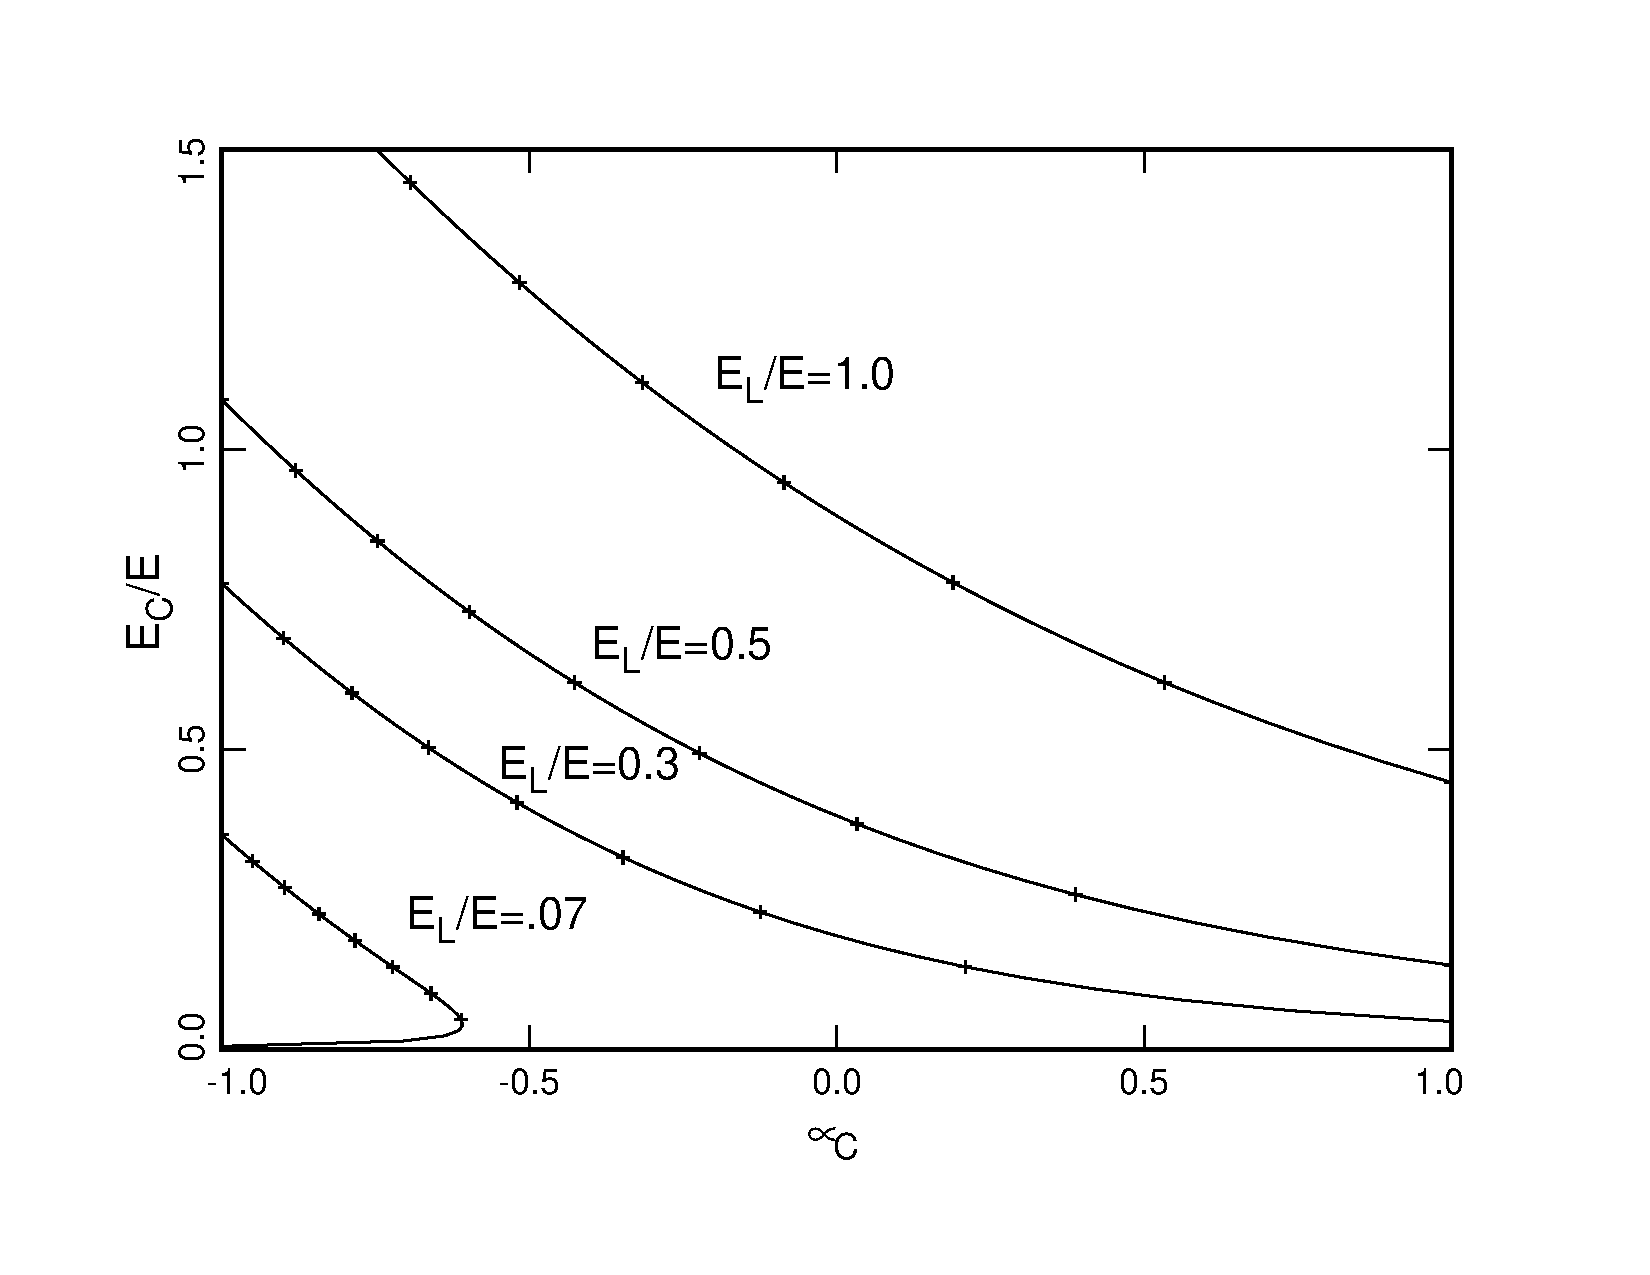
\includegraphics[keepaspectratio, height=3.5in, angle=0]{figs/groupr7ack}
\caption[Coordinate mapping between CM and LAB reference frames
 for A=2]{Coordinate mapping between CM and laboratory reference frames
 for A=2.  The parameters $E_L$ and $E_C$ are the secondary energies in the
 Lab and CM frames.  The crosses on the curves are at $\mu_L$ values of -1.0,
 -.75, -.50, \ldots, .75, and 1.0.  This figure also illustrates the advantage
 of integrating over $\mu_L$ for the contour in the lower-left corner.  The
 values of $E_C$ and $\mu_C$ are single-values functions of $\mu_L$.}
\label{transform}
\end{figure}

The CM energy-angle distribution can be given as a set of Legendre
coefficients or a tabulated angular distribution for each
possible energy transfer $E{\rightarrow}E'$, as a ``precompound fraction''
$r(E,E')$ for use with the
Kalbach-Mann\cite{km}\index{Kalbach-Mann systematics}
or Kalbach\cite{k86}\index{Kalbach systematics} angular
distributions, or as parameters for a phase-space\index{phase-space
distributions} distribution.  The first three options are processed using
\cword{f6ddx}\index{f6ddx@{\ty f6ddx}}, and the last using
\cword{f6psp}\index{f6psp@{\ty f6psp}}.  The Kalbach  option
leads to a very compact representation.  Kalbach and Mann examined
large number of experimental angular distributions for neutrons
and charged particles.  They noticed that each distribution could
be divided into two parts: an equilibrium part symmetric in $\mu$,
and a forward-peaked preequilibrium part.  The relative amount of
the two parts depended on a parameter $r$, the preequilibrium fraction,
\index{preequilibrium fraction} that varies from zero for low $E'$ to 1.0
for large $E'$.  The shapes of the two parts of the distributions
depended most directly on $E'$.  This representation is very useful
for preequilibrium statistical-model codes like
GNASH\cite{GNASH}\index{GNASH}, because they can compute the
parameter $r$, and all the rest of the angular information comes
from simple universal functions.   More specifically,
Kalbach's latest work says that

\begin{equation}
   f(\mu)=\frac{a}{2\sinh(a)}\Bigl[\cosh(a\mu)+r\sinh(a\mu)\Bigr],
\end{equation}

\noindent
where $a$ is a simple function of $E$, $E'$, and $B_b$, the separation
energy of the emitted particle from the liquid-drop model without
pairing and shell terms.  The separation energies\index{separation energy}
are computed by formulas in \cword{bach}\index{bach@{\ty bach}}.  There
is a problem for elemental evaluations, because the calculations needs
an A value for the element, and it is difficult to guess which A value
is most characteristic of the element.  A short table is included in
the routine, and an ``\cword{error in bach}'' will result if the
function is called for an element that doesn't appear
in the table.  Similar routines appear in
\hyperlink{sHEATRhy}{HEATR}\index{HEATR} and
\hyperlink{sACERhy}{ACER}\index{ACER}.  A better
long-range solution would be desirable.
Fortunately, elemental evaluations are rare in modern
evaluated libraries.

The File 6 processing methods in GROUPR apply equally well to
neutrons, photonuclear photons, and charged particles.  The effects
on the kinematics due to the difference in mass between the incident
particle and the emitted particle are handled by the variable $A'$ in
the above equations.

\subsection{Smoothing}
\label{ssGROUPR_Smooth}

For continuum CM distributions in File 6, the low-energy shape
should go like $\sqrt{E'_C}$\index{sqrt(E) shape}.  From Eq.~\ref{yy2},
we see that the low-energy shape for the Lab distribution would then go
like $\sqrt{E'_L}$.  However, ENDF/B-VII evaluations for File 6
were normally prepared using advanced nuclear model codes, such as
GNASH\index{GNASH} from LANL\index{Los Alamos National Laboratory!LANL}.  These
codes naturally produce spectra represented
with histogram bins, and these bins normally give a constant
probability from zero energy to the next bin boundary.  This
is certainly not a $\sqrt{E}$ shape!  The histogram shape can
cause trouble with the CM-Lab transformation if some care is not
taken.  Clearly, the histogram grossly overestimates the probability
of scattering to very low energies.  This apparent problem is somewhat
alleviated by the fact that the total probability of that lowest
histogram bin is usually quite small.  However, in order to get
better looking shapes, GROUPR has coding that replaces the
coarse histogram with a finer histogram chosen to represent a
$\sqrt{E}$ shape more closely.  This smoothing\index{smoothing}
coding scans up through the histogram distribution from the evaluation
to find the region that behaves like $\sqrt{E}$.  It then uses a
recursive procedure to subdivide the region using a given factor
until it reaches a fairly low energy (currently 40 eV).

A similar procedure is used to provide a $\sqrt{E}$ shape
at low energies for delayed neutron spectra.

For a few of the ENDF/B-VII\index{ENDF!ENDF/B-VII} actinides, the
energy grid used to represent the fission spectrum becomes too
coarse above 10 MeV.  If that situtation is found, GROUPR changes
the interpolation law from the given lin-lin option to
lin-log --- that is, an exponential tail is assumed for the
high energies.  This assumption is consistent with the orginal
evaluations.  This modification can be important for reaction
rates of high-threshold reactions.

These smoothing options are controlled by the global parameter
\cword{ismooth}\index{ismooth@{\ty ismooth}}, which is turned on
by default (in constrast to NJOY99 where it is turned off by default).


\subsection{GENDF Output}
\label{ssGROUPR_GENDF}

The group constants produced by GROUPR are normally written to
an output file in GENDF\index{GENDF} (groupwise ENDF) format
for use by other modules of NJOY.  For example,
\hyperlink{sDTFRhy}{DTFR}\index{DTFR}
can be used to convert a GENDF material to DTF (or ``transport'')
format; \hyperlink{sCCCCRhy}{CCCCR}\index{CCCCR} produces
the standard interface
files\cite{CCCC4} ISOTXS\index{ISOTXS}, BRKOXS\index{BRKOXS}, and
DLAYXS\index{DLAYXS}; \hyperlink{sMATXSRhy}{MATXSR}\index{MATXSR}
produces a file in MATXS\index{MATXS} format\cite{TRANSX};
and \hyperlink{sPOWRhy}{POWR}\index{POWR}
produces libraries for the Electric Power Research Institute
(EPRI)\index{EPRI} codes EPRI-CELL\index{EPRI!EPRI-CELL} and
EPRI-CPM\index{EPRI!EPRI-CPM}.  Other formats can easily be
produced by new modules, and some functions such as group collapse,
are conveniently performed directly in GENDF format.  The GENDF
format is also used for \hyperlink{sGAMINRhy}{GAMINR}\index{GAMINR}
output, and both \hyperlink{sACERhy}{ACER}\index{ACER} and
\hyperlink{sERRORRhy}{ERRORR}\index{ERRORR} use GENDF input for
some purposes.

Depending on the sign of \cword{ngout2} (see below), the GENDF file will
be written in either coded mode ({\it e.g.}, ASCII) or in the special
NJOY blocked-binary mode.  Conversion between these modes can be
performed subsequently by the
\hyperlink{sMODERhy}{MODER} module.\index{MODER}

The GENDF material begins with a header record (MF=1, MT=451), but the
format of this first section is different from MT=451 on an ENDF or
PENDF tape.  The section consists of a ``CONT'' record, containing

\begin{quote}
\centering
\begin{tabular}{ll}
\cword{ZA} &  Standard 1000*Z+A value \\
\cword{AWR} &  Atomic weight ratio to neutron \\
\cword{0} &  Zero \\
\cword{NZ} &  Number of $\sigma_0$ values \\
\cword{-1} &  Identifies a GENDF-type data file \\
\cword{NTW} &  Number of words in title
\end{tabular}
\end{quote}

\noindent
and a single ``LIST'' record, containing

\begin{quote}
\centering
\begin{tabular}{ll}
\cword{TEMPIN} &  Material temperature (Kelvin) \\
\cword{0.} &  Zero \\
\cword{NGN} &  Number of neutron groups \\
\cword{NGG} &  Number of photon groups \\
\cword{NW} &  Number of words in LIST \\
\cword{0} &  Zero \\
\cword{TITLE} &  Title from GROUPR input (\cword{NTW} words) \\
\cword{SIGZ} &  Sigma-zero values (\cword{NZ} words) \\
\cword{EGN} &  Neutron group boundaries, low to high (\cword{NGN}+1 words) \\
\cword{EGG} &  Photon group boundaries, low to high (\cword{NGG}+1 words).
\end{tabular}
\end{quote}

\noindent
For photoatomic GENDF files produced by the
\hyperlink{sGAMINRhy}{GAMINR} module, the
photon group structure is stored in \cword{ngn} and \cword{egn},
and the number of photon groups is given as \cword{ngg}=0.
The word count is NW=NTW+NZ+NGN+1+NGG+1.  The LIST record
is followed by a standard ENDF file-end record (FEND).  The normal
ENDF section-end (SEND) is omitted.

This header is followed by a series of records for reactions.
The ENDF ordering requirements are relaxed, and MF and MT values can
occur in any order.  Each section starts with a ``CONT'' record.

\begin{quote}
\centering
\begin{tabular}{ll}
\cword{ZA} &  Standard 1000*Z+A value \\
\cword{AWR} &  Standard atomic weight ratio \\
\cword{NL} &  Number of Legendre components \\
\cword{NZ} &  Number of sigma-zero values \\
\cword{LRFLAG} &  Break-up identifier flag \\
\cword{NGN} &  Number of groups
\end{tabular}
\end{quote}

\noindent
It is followed by a series of LIST records, one for every
incident-energy group with nonzero result,

\begin{quote}
\centering
\begin{tabular}{ll}
\cword{TEMP} &  Material temperature (Kelvin) \\
\cword{0.} &  Zero \\
\cword{NG2} &  Number of secondary positions \\
\cword{IG2LO} &  Index to lowest nonzero group \\
\cword{NW} &  Number of words in LIST \\
\cword{IG} &  Group index for this record \\
\cword{A(NW)} &  Data for LIST (NW words),
\end{tabular}
\end{quote}

\noindent
where \cword{NW}=\cword{NL}*\cword{NZ}*\cword{NG2}.  The last LIST record in
the sequence is the one with \cword{IG}=\cword{NGN}.  It must be given even
if its contents are zero.  The last LIST record is followed by a SEND record.

The contents of \cword{A(NW)} change for various types of data.  For simple
cross section ``vectors'' (MF=3), NG2 is 2, and A contains the two
Fortran arrays

\indent \cword{FLUX(NL,NZ), SIGMA(NL,NZ)}

\noindent
in that order.  For ratio quantities like fission $\overline\nu$,
\cword{NG2} is 3, and \cword{A} contains

\indent \cword{FLUX(NL,NZ), RATIO(NL,NZ), SIGMA(NL,NZ)}.

\noindent
For transfer matrices (MF=6, 16, 21, {\it etc.}), \cword{A} contains

\indent \cword{FLUX(NL,NZ), MATRIX(NL,NZ,NG2-1)}.

\noindent
The actual secondary group indices for the last index
of \cword{MATRIX} are usually \cword{IG2LO}, \cword{IG2LO}+1, {\it etc.},
using the GROUPR convention of labeling groups in order of increasing
energy.  If the low-energy part of the fission matrix (or the fission or
capture photon production matrices) uses the special format described in
Section~\ref{ssGROUPR_FissSource}, the spectrum will be found in a LIST
record with \cword{IG}=0
and the production cross section will be found in a series of records
with \cword{IG2LO}=0.  The group range for the spectrum ranges from
\cword{IG2LO} to \cword{IG2LO}+\cword{NG2}-1.  For \cword{IG2LO}=0, \cword{NG2}
will be 2 as for a normal cross section, and the two values will be the
flux for group \cword{IG} and the corresponding production
cross section.

Finally, for delayed neutron spectra (MF=5), \cword{NL} is used to index
the time groups, \cword{NZ} is 1, and there is only one incident energy
record (\cword{IG}=\cword{IGN}).  The array \cword{A} contains

\indent \cword{LAMBDA(NL), CHID(NL,NG2-1),}

\noindent where \cword{LAMBDA} contains the delayed-neutron time constants
and \cword{CHID} contains the spectra.

The GENDF material ends with a material-end (MEND) record, and the GENDF
tape ends with a tape-end (TEND) record.

\subsection{Running GROUPR}
\label{ssGROUPR_RunningGROUPR}

GROUPR's input instructions follow.  They are reproduced from the comment
cards at the beginning of the
2016.0
version of the GROUPR module.
Because the code changes from time to time, it is a good idea to
check these comment cards in the current version to obtain
up-to-date input instructions.
\index{GROUPR!GROUPR input}
\index{input!GROUPR}

\small
\begin{ccode}

   !---input specifications (free format)---------------------------
   !
   ! card1
   !    nendf   unit for endf tape
   !    npend   unit for pendf tape
   !    ngout1  unit for input gout tape (default=0)
   !    ngout2  unit for output gout tape (default=0)
   ! card2
   !    matb    material to be processed
   !             if ngout=0, matb<0 is an option to automatically
   !              process all the mats on the endf input tape.
   !             otherwise, matb<0 is a flag to add mts to and/or
   !              replace individual mts on gout1.
   !    ign     neutron group structure option
   !    igg     gamma group structure option
   !    iwt     weight function option
   !    lord    legendre order
   !    ntemp   number of temperatures (default=1)
   !    nsigz   number of sigma zeroes (default=1)
   !    iprint  long print option (0/1=minimum/maximum)
   !            (default=1)
   !    ismooth switch on/off smoothing operation (1/0, default=1=on)
   !            set ismooth to 1 to enable sqrt(e) smoothing for
   !            mf6 cm emission spectra at low energies and for
   !            histogram delayed neutron spectra at low energies.
   ! card3
   !    title   run label (up to 80 characters delimited by quotes,
   !            ended with /)  (default=blank)
   ! card4
   !    temp    temperatures in kelvin
   ! card5
   !    sigz    sigma zero values (including infinity)
   !
   !          if ign=1, read neutron group structure (6a and 6b)
   ! card6a
   !    ngn     number of groups
   ! card6b
   !    egn     ngn+1 group breaks (ev)
   !
   !          if igg=1, read gamma group structure (7a and 7b)
   ! card7a
   !    ngg     number of groups
   ! card7b
   !    egg     ngg+1 group breaks (ev)
   !
   !          weight function options (8a,8b,8c,8d)
   ! card8a     flux calculator parameters (iwt.lt.0 only)
   !    fehi    break between computed flux and bondarenko flux
   !            (must be in the resolved resonance range)
   !    sigpot  estimate of potential scattering cross section
   !    nflmax  maximum number of computed flux points
   !    ninwt   tape unit for new flux parameters (default=0)
   !            note: weighting flux file is always written binary
   !    jsigz   index of reference sigma zero in sigz array
   !            (default=0)
   !    alpha2   alpha for admixed moderator (def=o=none)
   !    sam      admixed moderator xsec in barns per absorber
   !             atom (def=0=none)
   !    beta     heterogeneity parameter (def=0=none)
   !    alpha3   alpha for external moderator (def=0=none)
   !    gamma    fraction of admixed moderator cross section in
   !              external moderator cross section (def=0)
   ! card8b     tabulated (iwt=1 or -1 only)
   !    wght    read weight function as tab1 record,
   !            this may span multiple lines and ends with a /.
   ! card8c     analytic flux parameters (iwt=4 or -4 only)
   !    eb      thermal break (ev)
   !    tb      thermal temperature (ev)
   !    ec      fission break (ev)
   !    tc      fission temperature (ev)
   ! card8d     input resonance flux (iwt=0 only)
   !    ninwt   tape unit for flux parameters (binary)
   !
   ! card9
   !    mfd     file to be processed
   !    mtd     section to be processed
   !    mtname  description of section to be processed
   !          repeat for all reactions desired
   !          mfd=0/ terminates this temperature/material.
   ! card10
   !    matd    next mat number to be processed
   !            matd=0/ terminates groupr run.
   !
   !---options for input variables----------------------------------
   !
   !     ign          meaning
   !     ---          -------
   !      1           arbitrary structure (read in)
   !      2           csewg 239-group structure
   !      3           lanl 30-group structure
   !      4           anl 27-group structure
   !      5           rrd 50-group structure
   !      6           gam-i 68-group structure
   !      7           gam-ii 100-group structure
   !      8           laser-thermos 35-group structure
   !      9           epri-cpm 69-group structure
   !     10           lanl 187-group structure
   !     11           lanl 70-group structure
   !     12           sand-ii 620-group structure
   !     13           lanl 80-group structure
   !     14           eurlib 100-group structure
   !     15           sand-iia 640-group structure
   !     16           vitamin-e 174-group structure
   !     17           vitamin-j 175-group structure
   !     18           xmas nea-lanl
   !     all new additional group structure with 7 significant
   !     decimal digits compatible with calendf
   !     19           ecco  33-group structure
   !     20           ecco 1968-group structure
   !     21           tripoli 315-group structure
   !     22           xmas lwpc 172-group structure
   !     23           vit-j lwpc 175-group structure
   !     24           shem cea 281-group structure
   !     25           shem epm 295-group structure
   !     26           shem cea/epm 361-group structure
   !     27           shem epm 315-group structure
   !     28           rahab aecl 89-group structure
   !     29           ccfe   660-group structure  (30 MeV)
   !     30           ukaea 1025-group structure  (30 MeV)
   !     31           ukaea 1067-group structure (200 MeV)
   !     32           ukaea 1102-group structure   (1 GeV)
   !     33           ukaea  142-group structure (200 MeV)
   !     34           lanl 618-group structure
   !
   !     igg          meaning
   !     ---          -------
   !      0           none
   !      1           arbitrary structure (read in)
   !      2           csewg 94-group structure
   !      3           lanl 12-group structure
   !      4           steiner 21-group gamma-ray structure
   !      5           straker 22-group structure
   !      6           lanl 48-group structure
   !      7           lanl 24-group structure
   !      8           vitamin-c 36-group structure
   !      9           vitamin-e 38-group structure
   !     10           vitamin-j 42-group structure
   !
   !     iwt          meaning
   !     ---          -------
   !      1           read in smooth weight function
   !      2           constant
   !      3           1/e
   !      4           1/e + fission spectrum + thermal maxwellian
   !      5           epri-cell lwr
   !      6           (thermal) -- (1/e) -- (fission + fusion)
   !      7           same with t-dep thermal part
   !      8           thermal--1/e--fast reactor--fission + fusion
   !      9           claw weight function
   !     10           claw with t-dependent thermal part
   !     11           vitamin-e weight function (ornl-5505)
   !     12           vit-e with t-dep thermal part
   !     -n           compute flux with weight n
   !      0           read in resonance flux from ninwt
   !
   !     mfd          meaning
   !     ---          -------
   !      3           cross section or yield vector
   !      5           fission chi by short-cut method
   !      6           neutron-neutron matrix (mf4/5)
   !      8           neutron-neutron matrix (mf6)
   !     12           photon prod. xsec (photon yields given, mf12)
   !     13           photon prod. xsec (photon xsecs given, mf13)
   !     16           neutron-gamma matrix (photon yields given)
   !     17           neutron-gamma matrix (photon xsecs given)
   !     18           neutron-gamma matrix (mf6)
   !         note: if necessary, mfd=13 will automatically change
   !         to 12 and mfd=16 will automatically change to 17 or 18.
   !     21           proton production matrix (mf6)
   !     22           deuteron production (mf6)
   !     23           triton production (mf6)
   !     24           he-3 production (mf6)
   !     25           alpha production (mf6)
   !     26           residual nucleus (a>4) production (mf6)
   !     31           proton production matrix (mf4)
   !     32           deuteron production (mf4)
   !     33           triton production (mf4)
   !     34           he-3 production (mf4)
   !     35           alpha production (mf4)
   !     36           residual nucleus (a>4) production (mf4)
   !          note: if necessary, mfd=21-26 will
   !          automatically change to 31-36.
   !    1zzzaaam       nuclide production for zzzaaam
   !                     subsection from file 3
   !    2zzzaaam       nuclide production for zzzaaam
   !                     subsection from file 6
   !    3zzzaaam       nuclide production for zzzaaam
   !                     subsection from file 9
   !    4zzzaaam       nuclide production for zzzaaam
   !                     subsection from file 10
   !    40000000       fission product production (mtd=18 only)
   !                     subsection from file 10
   !
   !     mtd          meaning
   !     ---          -------
   !     -n           process all mt numbers from the previous
   !                          entry to n inclusive
   !     221-250      reserved for thermal scattering
   !     257          average energy
   !     258          average lethargy
   !     259          average inverse velocity (m/sec)
   !
   !     automatic reaction processing options
   !     -------------------------------------
   !        3/        do all reactions in file3 on input pendf
   !        6/        do all matrix reactions in endf dictionary
   !       10/        do all isotope productions using mf8
   !       13/        do all photon production cross sections
   !       16/        do all photon production matrices
   !       21/        do all proton production matrices
   !       22/        do all deuteron production matrices
   !       23/        do all triton production matrices
   !       24/        do all he-3 production matrices
   !       25/        do all alpha production matrices
   !       26/        do all a>4 production matrices
   !
   !-------------------------------------------------------------------

\end{ccode}
\normalsize

In these instructions, \cword{card1} defines the input and output units
for GROUPR.  The module requires both ENDF and PENDF input tapes,
because the PENDF tapes produced by
\hyperlink{sRECONRhy}{RECONR}\index{RECONR},
\hyperlink{sBROADRhy}{BROADR}\index{BROADR} {\it etc.}, do not
contain angle (MF=4),
energy (MF=5), or photon (MF=12, 15) distributions.  For materials
that do not use resonance parameters to represent part of the
cross section, it is possible to use a copy of the ENDF tape in place
of the PENDF tape.  The normal mode for GROUPR is to use \cword{ngout1}=0;
however, sometimes it is convenient to add a new material or reaction to
an existing GENDF tape.  The old GENDF tape is then mounted on unit
\cword{ngout1}, and the revised GENDF tape will be written to \cword{ngout2}.

Card 2 selects the first material to be processed (\cword{matb}) and sets
up the group structures\index{group structures},
weighting option\index{weight functions}, Legendre order, and
self-shielding\index{self-shielding} parameters for all the materials
to be processed in this run.

The names of the available group structures are given in the input
instructions. Energy bounds or lethargy bounds can be found in the
source code.  Of course, it is always possible to read in an arbitrary
group structure (see \cword{card6a} through \cword{card7b}).  The energies
must be given in increasing order (note that this is opposite from the
usual convention).  Here is an example of the input cards for the
conventional 4-group structure historically used in some thermal
reactor codes:
\index{4-group structure}

\small
\begin{ccode}

   4/ card6a
   1e-5 .625 5530 .821e6 10e6 / card6b

\end{ccode}
\normalsize

\noindent
These cards are read by the standard Fortran READ* method.
Fields are delimited by space, and ``/'' terminates the processing
of input on a card.  Anything after the slash is a comment.

\begin{figure}[t]\centering
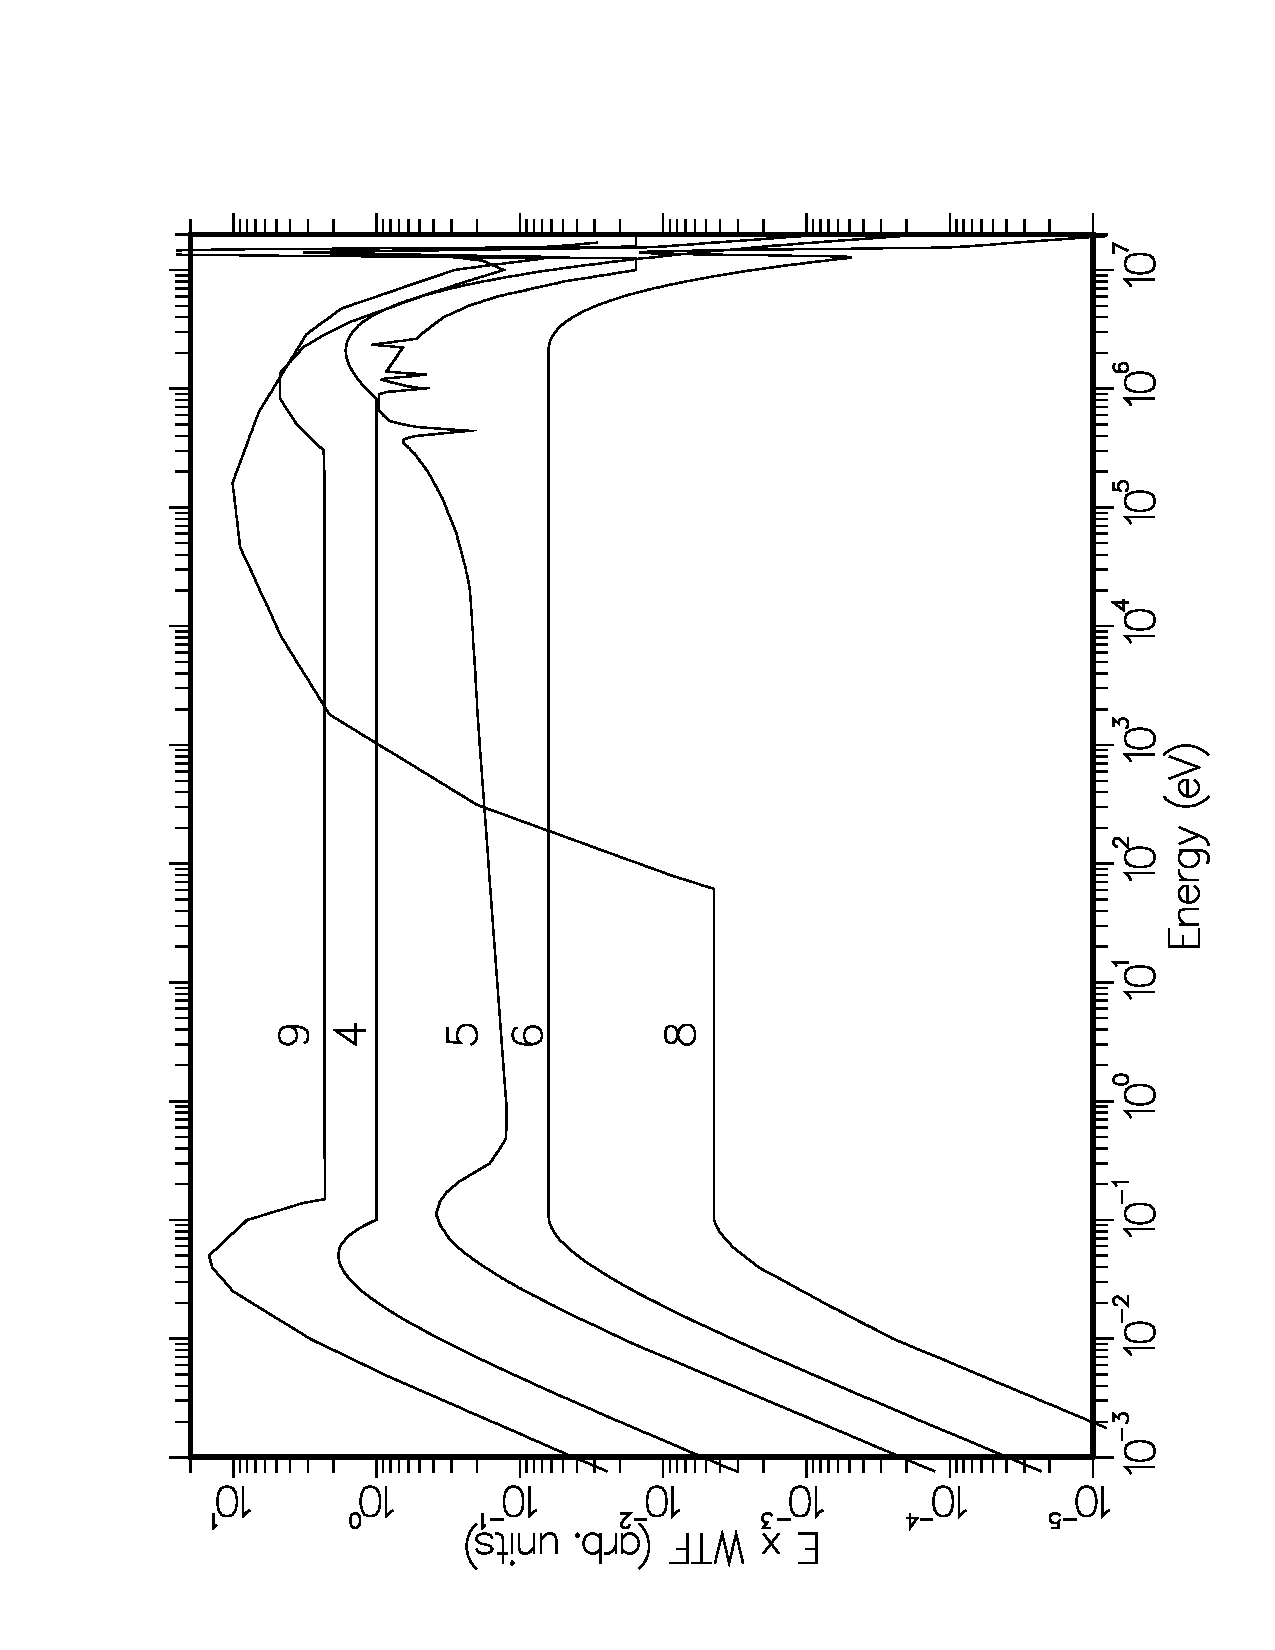
\includegraphics[keepaspectratio, height=3.9in, angle=270]{figs/appb1ack}
\caption[GROUPR weight functions on a logarithmic flux/unit lethargy
 scale]{Built-in neutron weight functions of GROUPR on a logarithmic
 flux-per-unit-lethargy plot that emphasizes the low energy range.}
\label{fig-leth}
\end{figure}

The available weight function options are listed in the input
instructions under \cword{iwt}.  See Fig.~\ref{fig-leth} and
Fig.~\ref{fig-lin}.  Here are brief descriptions of the options:

\begin{figure}[t]\centering
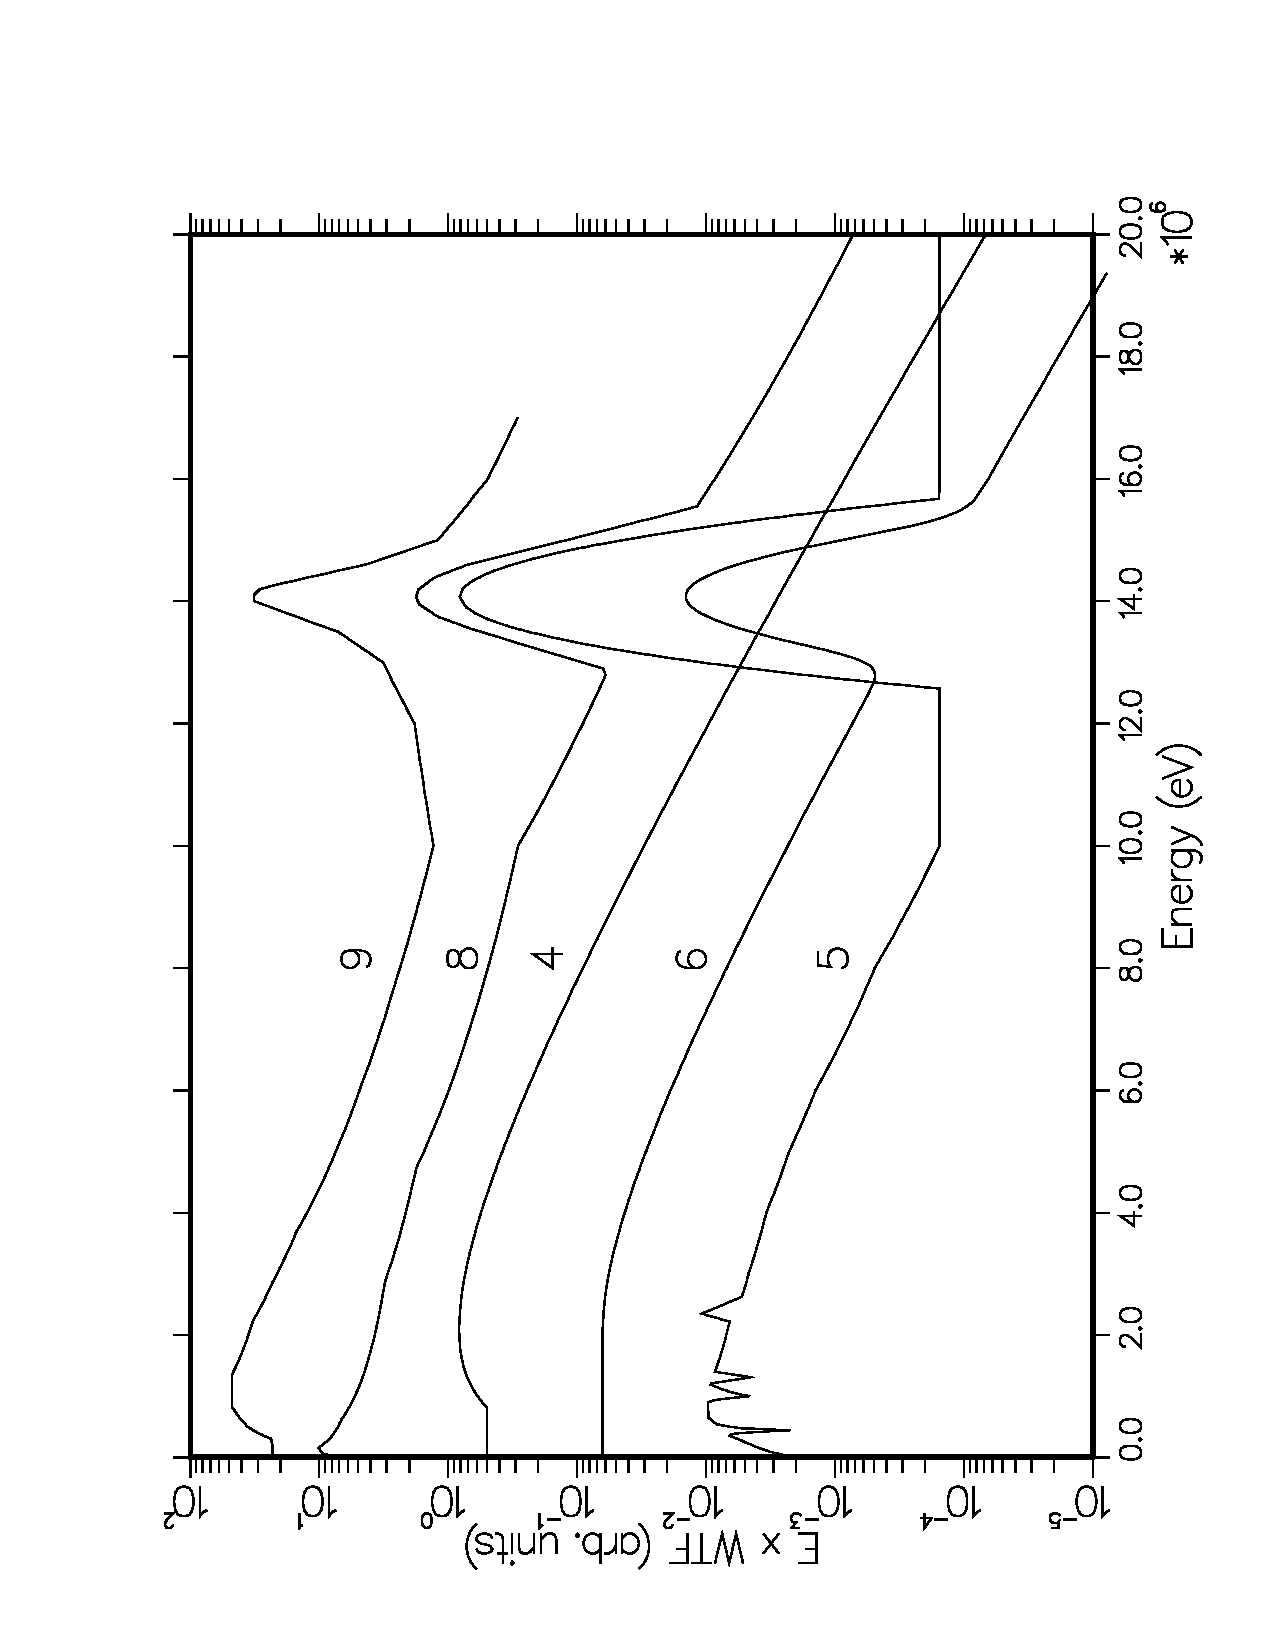
\includegraphics[keepaspectratio, height=3.9in, angle=270]{figs/appb2ack}
\caption[GROUPR weight functions on a linear energy scale]{Built-in neutron
 weight functions on a linear plot that emphasizes the high-energy range.}
\label{fig-lin}
\end{figure}

\begin{description}
\begin{singlespace}
\item{IWT=2\ } The weight function is constant (not shown in the Figures).
   This option is usually chosen for very fine group
   structures such as the 620-group or 640-group
   dosimetry structures.

\item{IWT=3\ } The weight function is proportional to $1/E$.
   The slowing-down of neutrons in water gives a $1/E$
   flux from about 1 eV up to 100 keV, or so.  This
   weight function is traditionally used for
   calculating resonance integrals, but it is not
   useful at the lower and higher energies needed for a
   full set of transport constants.  Although not shown, the graph
   of this function is a flat line on a flux-per-unit-lethargy
   plot, such as the one in Fig.~\ref{fig-leth}.

\item{IWT=4\ } This weight function combines a thermal Maxwellian at low
   energies, a $1/E$ function at intermediate energies, and a
   fission spectrum at high energies to obtain a function appropriate
   for several different applications.  The temperatures of the
   Maxwellian and fission parts and the energies where the components
   join can be chosen by the user.  Therefore, option 4 can be used
   to produce typical thermal reactor weight functions like those
   shown in Figures~\ref{fig-leth} and \ref{fig-lin}, a pure fission
   spectrum for calculating some kinds of dosimetry cross sections, or a
   pure thermal spectrum for getting effective thermal average cross
   sections.  The function  for IWT=4 shown in the figure was produced
   using a thermal temperature of 0.025 eV joined to $1/E$ at 0.1~eV,
   and a fission temperature of 1.40 MeV joined to $1/E$ at 820.3 keV.

\item{IWT=5\ } This is a mid-life PWR (pressurized water reactor) flux
   spectrum with a fusion peak added (see below for a discussion of the
   fusion peak used).  Note the peaks and dips resulting from oxygen
   resonances and windows at high energies, and the hardening apparent
   in the epithermal region.  The thermal part of the function is also
   hardened with respect to a simple Maxwellian shape.  The dips that
   should show up in the eV range due to resonances and $^{238}$U have been
   removed to allow the self-shielding method to work without risk of
   counting the shielding effects twice.  This weight function has
   been used for several libraries\cite{powr} prepared for the Electric
   Power Research Institute (EPRI)\index{EPRI}, and for the MATXS7 library
   used with the TRANSX code\index{TRANSX}.

\item{IWT=6\ } This function is similar to option 4, but the breakpoints
   were chosen to keep the curves continuous.  The thermal Maxwellian
   is calculated for 300K.  In this case, the fusion peak (see below)
   was added to the high-energy tail of the fission spectrum for
   smoothness.

\item{IWT=7\ }  This option is reserved for future use.

\item{IWT=8\ } This function is intended for cross sections libraries
   used for fast reactor analysis (typically, fast breeder
   designs), but is also useful for fusion-blanket problems.  It has
   a fusion peak at high energies, followed by a fission spectrum, a
   slowing-down spectrum typical of a fast reactor, and a thermal tail.
   The tail is provided to help give reasonable results in shields
   far from the core; its characteristic temperature is 300K.  Note
   the sharp drop in the flux as energy decreases from 19 keV.  This
   region is important for $^{238}$U absorption, and this drop-off helps
   to give good group constants for fast reactors.  Of course, it
   would be entirely wrong for a thermal reactor.

\item{IWT=9\ } This is another typical thermal+$1/E$+fission+fusion
   function that has been used for many libraries at LANL
   in the 30-group structure.  The CLAW-3 and
   CLAW-4 libraries are available from the Radiation Shielding
   Information Computational Center at ORNL.

\item{IWT=10\ } This is the same as the CLAW weight function
   (IWT=9), but the shape of the thermal part is automatically
   recalculated to follow a Maxwellian law for temperature $T$.

\item{IWT=11\ } This is the weight function used in the
   VITAMIN-E library.  It has the following segments:
   a .0253-eV thermal Maxwellian below 0.414 eV, a $1/E$ law from
   .414 eV to 2.12 MeV, a 1.415-MeV fission spectrum from 2.12 to
   10 MeV, another $1/E$ section from 10 to 12.52 MeV, a fusion
   peak (25 keV width) between 12.52 and 15.68 MeV, and a final
   $1/E$ section for all higher energies.  The shape of the fusion
   peak is almost identical to IWT=5 (see Fig.~\ref{fig-lin}).  The
   low-energy part of this weight function is not shown.
\end{singlespace}
\end{description}

\noindent
Just as in the case of group structures, an arbitrary weight
function can be read in (see \cword{card8b}).  This function is
presented to GROUPR as an ENDF/B ``TAB1'' record.  This means that a
count of $E,C(E)$ pairs and one or more interpolation schemes are given.

An ENDF/B ``TAB1'' record consists of three distinct parts:
\begin{itemize}
\item two double values and four integer values of which only the last
two integers (the number of interpolation ranges \cword{NR} and the number
of $E,C(E)$ pairs \cword{NP}) are needed to read the remainder of the record
\item the interpolation scheme data which is a sequence of \cword{NR} pairs
of \cword{NBT} (index of the $E,C(E)$ pair corresponding to the end of
interpolation range) and \cword{INT} (the interpolation type)
\item the tabulated data which is a sequence of \cword{NP} $E,C(E)$ pairs
\end{itemize}

\noindent
The interpolation type \cword{INT} specifies the interpolation law to be used in the
interpolation range. It can take the following values:

\begin{center}
\begin{tabular}{cl}
\cword{INT} & Meaning \\ \hline
1 & histogram\\
2 & linear-linear\\
3 & linear-log\\
4 & log-linear\\
5 & log-log \\ \hline
\end{tabular}
\end{center}

\noindent
For example, \cword{INT}=5 specifies that ln$C$ is a linear function of ln$E$.
Similarly, INT=4 specifies that ln$C$ is a linear function of $E$.

\noindent
In its most general form, these input cards would be

\small
\begin{ccode}

   0.      0.      0       0       NR      NP
   NBT(1)  INT(1)    ...   NBT(NR) INT(NR)
   E(1)    C(1)      ...   E(NP)   C(NP)        / card8b

\end{ccode}
\normalsize

\noindent
For example, a function using two interpolation ranges: the first one
between 1e-5 eV and 100 eV using a histogram and the second one between
100 eV and 20 MeV using lin-lin interpolation)

\small
\begin{ccode}

   0.      0.      0       0       2       6
   3       1       6       2
   1e-5    0.5     1.      0.75    100.    0.8
   1e+6    0.85    1.5e+6  0.9     2.0e+7  1.0  / card8b

\end{ccode}
\normalsize

\noindent
For the special case of a single interpolation scheme, the input cards
are simplified as follows

\small
\begin{ccode}

   0.      0.      0       0       1       NP
   NP      INT
   E(1)    C(1)      ...   E(NP)   C(NP)        / card8b

\end{ccode}
\normalsize

\noindent
As many physical lines as are needed can be used for ``\cword{card8b}'',
as long as the terminating slash is included.

One of the weighting options, IWT=4, is a generalized
``$1/E$+fission+thermal'' function where the thermal temperature,
fission temperature, and breakpoint energies (all in eV) are given
on \cword{card8c}.  The weight function for the Los Alamos LIB-IV
cross section library\cite{LIBIV} used
\index{LIB-IV}

\small
\begin{ccode}

   .10 .025 820.3e3 1.4e6 / card8c

\end{ccode}
\normalsize

\noindent
See Figures~\ref{fig-leth} and \ref{fig-lin} for a plot of this function.

Several of these weight functions include a fusion peak\index{fusion peak}.
Because of the finite width of the distribution of ion
energies in a D-T fusion plasma, the emitted 14-MeV
neutrons clearly will not have a delta-function energy
spectrum.  In fact, owing to the presence of a cross-product
term in the kinematic relations, the typical ion-energy
spread of a few tens of kilovolts is magnified into a
neutron-energy spread of around 1 MeV.
For an assumed isotropic Maxwellian plasma, the neutron peak
shape (for example, see the review article by Lehner\cite{one}) is

\begin{equation}
  S(E)=C\int_0^\infty \exp\{-b\bigl[v^2+v_0(g)^2\bigr]-cg^2\}
  \sinh(2bvv_0)\,{{g^3\sigma(g)}\over{v_0(g)}}\,dg \,\,.
\label{lehner}
\end{equation}

\noindent
Here $S(E)$ is the number of neutrons emitted with laboratory
energy between $E$ and $E+dE$, $C$ is a normalization
factor, $v$ is the laboratory velocity corresponding to
energy $E$, and $v_0$ is the velocity of the neutron in
the CM system.  Both $v_0$ and the fusion cross section
$\sigma$ are determined by the relative velocity $g$ of
the reacting ions, the integration variable in Eq.~\ref{lehner}.
The coefficient $b$ is equal to $M/2kT$, where $M$ is the
total mass of the reacting ions and $kT$ is the plasma
temperature.  Similarly, $c$ is $\mu /2kT$, where $\mu$
is the reduced mass of the ion system.
The only approximation involved in Lehner's derivation
of Eq.~\ref{lehner} is that all particles may be treated
nonrelativistically.  At 14 MeV, the relativistic factor

\begin{equation}
  \gamma={{1}\over{\sqrt{1-v^2/c^2}}}\,\,,
\end{equation}

\noindent
is very close to unity (1.015), and it varies negligibly over
the range of interest (say, 13 to 17 MeV).  It is sufficient
then to invoke relativistic mechanics in defining the location
of the 14-MeV peak but not in discussing the shape.  This
effect  moves the peak toward lower neutron energies, but
only by about 20 keV.  Although the expression for $S(E)$
in Eq.~\ref{lehner} is accurate, it has the disadvantage of
requiring a numerical integration at each point $E$ in the
energy spectrum.  For this reason, we consider what
simplifications can be made without serious loss
of accuracy.  In the energy range around the 14-MeV peak, the
product $2bvv_0$ in Eq.~\ref{lehner} has a numerical value of
about 6000.  Thus, the hyperbolic sine can obviously be replaced
by just the positive exponential term.  If we make this change in
Eq.~\ref{lehner}, we can write the following, still nearly exact,
expression for the neutron spectrum:

\begin{equation}
  S_1(E)=C_1 \int_0^\infty \exp[-b(v-v_0)^2]\,P(v_0)\,dv_0 \,\,.
\label{intexp}
\end{equation}

\noindent
Here we also have inverted the function $v_0(g)$ and changed the
integration variable.  The spectrum then is a linear superposition
of velocity exponentials with slightly different peak locations.
For normal plasma temperatures, the velocity distribution
$P(v_0)$ is very narrow, since the expression for $v_0$ is
dominated by the nuclear Q-value (17.586 MeV) rather than the
contribution from the ion kinetic energy (typically around
50 keV).  Thus, it seems reasonable to approximate $P(v_0)$ as
delta function

\begin{equation}
  P(v_0) \approx \delta(v_0-v_p) \,\,.
\end{equation}

\noindent
This gives a second approximate form,

\begin{equation}
  S_2(E)=C_2 \exp[-b(v-v_p)^2] \,\,,
\label{velexp}
\end{equation}

\noindent
where $v_p$ has the obvious meaning of the laboratory neutron
velocity at the center of the peak.  We shall refer to this as
the velocity exponential form of the neutron energy spectrum.
An expression essentially identical to Eq.~\ref{velexp} was
given in an early paper by Nagle and coworkers\cite{two}.
In order to examine the accuracy of the velocity exponential form,
we have calculated $S(E)$ from Eq.~\ref{lehner}
and $S_2(E)$ from Eq.~\ref{velexp}
at 20 keV, a typical plasma temperature in current fusion-reactor
concepts.  In performing the numerical integration over $g$ in
Eq.~\ref{lehner}, we used numerical values for the D-T fusion cross
section taken from the compilation by Jarmie and Seagrave\cite{three}.
In evaluating $S_2(E)$ using Eq.~\ref{velexp}, a value of $v_p$ was
chosen so as to force agreement between $S_2(E)$ and $S(E)$ at
17 MeV.  As discussed by Muir\cite{four}\index{Muir}, the overall
agreement is remarkably good, the maximum error
over the range from 13.5 to 17 MeV being about 2\%.  The value of
$v_p$ thus derived corresponds to a peak-center energy $E_p$
of 14.07 MeV.  This value includes the small ($\sim$ 20 keV)
relativistic correction mentioned above.  If we approximate the
mass of the D{+}T system as 5 times the neutron mass, then we
obtain the recommended peak shape

\begin{equation}
  S_{\rm rec}(E)=\exp \bigl[ -{5 \over{kT}}(\sqrt{E}
  -\sqrt{E_p})^2 \bigr] \,\,,
\label{muir}
\end{equation}

\noindent
where $E_p{=}14.07\,{\rm MeV}$.  The functional form in Eq.~\ref{muir}
was used to calculate the fusion peak shapes appearing in two
of the data statements in \cword{genwtf}\index{genwtf@{\ty genwtf}}
(namely, those utilized for IWT=5 and 8) and  is also  used explicitly
in \cword{getwtf}\index{getwtf@{\ty getwtf}} to calculate analytically
the weight function for IWT=6.  In all three cases, $kT$=25 keV is
used as an average or typical fusion-reactor plasma temperature.
See Fig.~\ref{fig-lin} for a graphical display of the resulting
weight functions in the 14-MeV region.

The GROUPR flux calculator\index{flux calculator} is selected by
a negative sign on \cword{iwt}.  The additional \cword{card8a} is
then read.  The calculator option used is determined by the number
of parameters given and their values.  The parameters \cword{fehi}
and \cword{nflmax} are used to select the energy range for the
flux calculation, and they also determine the cost in time
and storage.  The actual value for \cword{sigpot} is not very
critical -- a number near 10 barns is typical for fissionable materials.

Nonzero values for \cword{ninwt} and \cword{jsigz} will cause the
computed flux for a given fissionable isotope (such as $^{238}$U) to be
written out onto a file.  This saved flux can be used as input for a
subsequent run for a fissile material (such as $^{239}$Pu) with
\cword{iwt}=0 to get an approximate correction for resonance-resonance
interference.  See Eq.~\ref{Eq38}.

Nonzero values for some of the last five parameters on \cword{card8a}
select the extended flux calculation of Eq.~\ref{Eq37}.  The simplest
such calculation is for an isolated pin containing a heavy absorber
with an admixed moderator.  For $^{238}$UO$_2$, the card might be

\small
\begin{ccode}

   400 10.6 5000 0 0 .7768 7.5 / card8a

\end{ccode}
\normalsize

\noindent
where 7.5 barns is twice the oxygen cross section and $\alpha$ is computed
from $\bigl[ (A-1)/(A+1)\bigr] ^2$ with $A=15.858$.  A more general case
would be a PWR-like lattice of $^{238}$UO$_2$ fuel rods in water:

\small
\begin{ccode}

   400 10.6 5000 0 0 .7768 7.5 .40 1.7e-7 0.086 / card8a

\end{ccode}
\normalsize

\noindent
where 0.086 is computed using 3.75 barns for O and 40 barns for the
two H atoms bound in water; that is,

\begin{equation}
  \gamma = \frac{3.75}{2*20 + 3.75}  = 0.086\;.
\end{equation}
\vspace{0.5 pt}

\noindent
A third example would compute the flux for a homogeneous mixture of
$^{238}$U and hydrogen

\small
\begin{ccode}

   400 10.6 5000 0 0 0 0 1. 1.7e-7 / card8a

\end{ccode}
\normalsize

\noindent
As a final example, consider a homogeneous mixture of uranium and water.
This requires \cword{beta}=1 and \cword{sam}=0.  Thus,

\small
\begin{ccode}

   400 10.6 5000 0 0 .7768 0. 1. 1.7e-7 .086 / card8a

\end{ccode}
\normalsize

The maximum Legendre expansion order used for scattering matrices is set
by \cword{lord}.  The number of tables produced is \cword{lord}+1; that is,
$\ell=0$, 1, ... \cword{lord}.  When more than 1 value of $\sigma_0$
is requested, both the $\ell{=}0$ and $\ell{=}1$ components of the
total cross section are produced.

Card 3 contains a short descriptive title that is printed on the listing
and added to the output GENDF tape.  Card 4 gives the \cword{ntemp} values
of temperature for the run.  They must be in ascending order, and if
unresolved data are included on the PENDF tape, the temperatures in this
list must match the first \cword{ntemp} values in MF=2, MT=152 from
\hyperlink{sUNRESRhy}{UNRESR}\index{UNRESR} or
\hyperlink{sPURRhy}{PURR}\index{PURR} (see
\cword{stounr}\index{stounr@{\ty stounr}} and
\cword{getunr}\index{getunr@{\ty getunr}}).  Card 5 gives the
$\sigma_0$ values for the run in descending order, starting with
infinity (represented by $10^{10}$ barns).

This completes the description of the global input parameters for GROUPR.
The rest of the input cards request reactions to be processed for the
various temperatures and materials desired.  Because of the many types
of data that it can process, GROUPR does not have a completely
automatic mode for choosing reactions to be processed.  On the basic
level, it asks the user to request each separate cross section or
group-to-group matrix using the parameters \cword{mfd}, \cword{mtd},
and \cword{mtname}.  However, simplified input modes are also available.
For example, the one ``\cword{card9}'' containing

\small
\begin{ccode}

    3/

\end{ccode}
\normalsize

\noindent
will process the cross section ``vectors'' for all of the reaction MT
numbers found on the PENDF tape.

For completeness, the full input for \cword{matd}, \cword{mfd},
and \cword{mtname} will be described first.  Most readers can skip
to the description of automated processing below.  The value of
\cword{mfd} depends on the output desired (vector, matrix) and the
form of the data on the ENDF evaluation.  Simple cross section ``vectors''
$\sigma_{xg}$ are requested using \cword{mfd}=3 and the \cword{mtd}
numbers desired from the list of reactions available in the evaluation
(check the directory in MF=1,MT=451 of the ENDF and PENDF tapes for the
reactions available).  A typical example would be

\small
\begin{ccode}

   3   1 'total'/
   3   2 'elastic'/
   3  16 '(n,2n)'/
   3  51 '(n,nprime)first'/
   3 -66 '(n,nprime)next'/
   3  91 '(n,nprime)continuum'/
   3 102 'radiative capture'/

\end{ccode}
\normalsize

\noindent
The combinations of ``3 51'' followed by ``3 $-$66'' means process all
the reactions from 51 through 66; that is, (n,n$'_1$), (n,n$'_2$),
\ldots, (n,n$'_{16}$).  If self-shielding is requested, the following
reactions will be processed using \cword{nsigz} values of background
cross section: total (MT=1), elastic (MT=2), fission (MT=18 and 19),
radiative capture (MT=102), heat production (MT=301), kinematic KERMA
(MT=443), and damage energy production (MT=444).  The other File-3
reactions will be computed at $\sigma_0{=}\infty$ only.  This list of
reactions can be altered by small changes in \cword{init} if desired.

There are several special options for \cword{mtd} available when processing
cross section vectors:

\begin{list}{ }{\labelsep=.25in\leftmargin=1in\labelwidth=.75in}
\begin{singlespace}
\item[\underbar{\cword{mtd}}] \underbar{Option}
\item[259] Average inverse neutron velocity for group in s/m.
\item[258] Average lethargy for group.
\item[251] Average elastic scattering cosine $\overline\mu$
               computed from File 4.
\item[252] Continuous-slowing-down parameter $\overline\xi$
               (average logarithmic energy decrement for elastic
               scattering) computed from File 4.
\item[253] Continuous-slowing-down parameter $\overline\gamma$
               (the average of the square of the logarithmic energy
               decrement for elastic scattering, divided by twice the
               average logarithmic energy decrement for elastic
               scattering) computed from File 4.
\item[452] $\overline\nu$: the average total fission yield
               computed from MF=1 and MF=3.
\item[455] $\overline\nu^D$: the average delayed neutron yield
               computed from MF=1 and MF=3.
\item[456] $\overline\nu^P$: the average prompt fission neutron
               yield computed from MF=1 and MF=3.
\end{singlespace}
\end{list}

\noindent
There are also some special options for \cword{mfd} that can
be used when processing cross sections:

\begin{list}{ }{\labelsep=.25in\leftmargin=1in\labelwidth=.75in}
\begin{singlespace}

\item[\underbar{\cword{mfd}}] \underbar{Option}
\item[12] Photon production cross section computed from File 12 and File 3.
\item[13] Photon production cross section computed from File 13.
          Recent versions of GROUPR will automatically shift
          between 12 and 13, if necessary.
\item[1zzzaaam] nuclide production for zzzaaam from a subsection of MF=3
\item[2zzzaaam] nuclide production for zzzaaam from a subsection of MF=6
\item[3zzzaaam] nuclide production for zzzaaam from a subsection of MF=9
\item[4zzzaaam] nuclide production for zzzaaam from a subsection of MF=10
\item[40000000] fission product production from the MT=18 subsection of MF=10
\end{singlespace}
\end{list}

\noindent
An example of the isomer production capability would be the
radiative capture reaction of ENDF/B-V $^{109}$Ag(n,$\gamma$)
from Tape 532:

\small
\begin{ccode}

   30471090 102 '(n,g) TO g.s.'/
   30471091 102 '(n,n) to isomer'/

\end{ccode}
\normalsize

\noindent
Starting with ENDF/B-VIII.0, some non-fissile nuclides can have an MT=18 section (fission)
in MF=10 (radioactive isotope production) to represent breakup due to high energy
particles. In these cases, it is often not possible to designate a specific nuclide,
which is why the \cword{mfd} value is set to \cword{40000000}. In such a case, the
following input will make GROUPR process this part of the ENDF file:

\small
\begin{ccode}

   40000000  18 'HE breakup' /

\end{ccode}
\normalsize

The next class of reactions usually processed is the group-to-group
neutron scattering matrices.  The complete list of \cword{mtd} values is
most easily found under File 4 in the MF=1,MT=451 ``dictionary''
section of the evaluation.  An example follows:

\small
\begin{ccode}

   6   2 'elastic matrix'/
   6  16 '(n,2n) matrix'/
   6  51 '(n,nprime)first matrix'/
   6 -66 '(n,nprime)next matrix'/
   6  91 '(n,nprime)continuum matrix'/  .

\end{ccode}
\normalsize

\noindent
Using \cword{mfd}=6 implies that File 4, or File 4 and File 5, will
be used to generate the group-to-group matrix.  The elastic matrix will
be computed for \cword{nsigz} values of background cross section, but
the other reactions will be computed for $\sigma_0{=}\infty$ only.  The
list of matrices to be self-shielded can be altered by changing
\cword{init}.

Fission is more complex.  For the minor isotopes, only
the total fission reaction is used, and the following input is appropriate
for the prompt component:

\small
\begin{ccode}

   3 18 'fission xsec'/
   6 18 'prompt fission matrix'/

\end{ccode}
\normalsize

\noindent
For the important isotopes, partial fission reactions are given.  They
are really not needed for most fission reactor problems, and the input
above is adequate.  However, for problems where high-energy neutrons
are important, the following input should be used:

\small
\begin{ccode}

   3 18 'total fission'/
   3 19 '(n,f)'/
   3 20 '(n,nf)'/
   3 21 '(n,2nf)'/
   3 38 '(n,3nf)'/
   6 19 '(n,f)'/
   6 20 '(n,nf)'/
   6 21 '(n,2nf)'/
   6 38 '(n,3nf)'/

\end{ccode}
\normalsize

\noindent
Note that ``6 18'' is omitted because it will, in general, be different
from the sum of the partial matrices (see Section~\ref{ssGROUPR_FissSource}).
Some materials don't have data for (n,3nf); in these cases, omit the two
lines with \cword{mtd}=38 from the input.  The fission matrix is not
self-shielded.  Since resonance-to-resonance fission-spectrum variations
are not described in the ENDF format, it is sufficient to self-shield
the cross section and then to use the self-shielding factor for the
cross section to self-shield the fission neutron production.

Delayed fission data are available for the important actinide isotopes,
and the following input to GROUPR is used to process them:

\small
\begin{ccode}

   3 455 'delayed nubar'/
   5 455 'delayed spectra'/

\end{ccode}
\normalsize

\noindent
The line for \cword{mfd}=5 automatically requests spectra for all time groups
of delayed neutrons.  The time constants are also extracted from
the evaluation.  As discussed in Section~\ref{ssGROUPR_FissSource},
formatting modules such as \hyperlink{sDTFRhy}{DTFR} and
\hyperlink{sCCCCRhy}{CCCCR} must combine the prompt and delayed
fission data written onto the GENDF tape in order to obtain steady-state
fission parameters for use in transport codes.

Starting with the ENDF-6 format, neutron production data may also be
found in File 6, and \cword{mfd}=8 is used to tell the code
to use MF6 for this \cword{mtd}.  When using full input, the user
will have to check the File 1 directory and determine what subsections
occur in File 6.

Photon production reactions can be found in the ENDF dictionary under
MF=12 and 13.  To request a neutron-to-photon matrix, add 4 to this
number.\footnote{In recent versions of NJOY, GROUPR will automatically
shift between 16 and 17 using data read from the ENDF dictionary by
the \cword{conver} subroutine.  Thus, use of \cword{mfd}=17 is no longer
necessary.}  For example,

\small
\begin{ccode}

   17   3 'nonelastic photons'/
   16   4 'inelastic photons'/
   16  18 'fission photons'/
   16 102 'capture photons'/

\end{ccode}
\normalsize

\noindent
Yields (MF=12) are normally used with resonance reactions (MT=18 or MT=102),
or for low-lying inelastic levels (MT=51, 52, ....).  MT=3 is often used
by evaluators as a catch-all reaction at high energies where it is
difficult to separate the source reactions in total photon emission
measurements.  In these cases, photon production cross sections from
other reactions like MT=102 are normally set equal to zero at high
energies.  The general rule for photon emission is that the total
production is equal to the sum of all the partial production reactions
given in the evaluation.   Starting with the ENDF-6 format, photon
production may also appear in File 6.  Use \cword{mfd=18} to process
these contributions.  Since resonance-to-resonance variations in
photon spectra are not given in ENDF evaluations, GROUPR does not normally
self-shield the photon production matrices (although this can be done
if desired by making a small change in \cword{init}); instead, it is
assumed that only the corresponding cross section needs to be shielded.
Subsequent codes can use the cross section self-shielding factor with the
infinite-dilution photon production matrix to obtain self-shielded photon
production numbers.

This version of GROUPR can also generate group-to-group matrices for
charged-particle production from neutron reactions and for all kinds
of matrices for incident charged particles.  The incident particle is
determined by the input tape mounted.  The identity of the secondary
particle is chosen by using one of the following special \cword{mfd}
values:

\begin{center}
For distributions given in File 6 (energy-angle):
\vspace{6 pt}
\begin{tabular}{cl}
  \cword{  mfd  } & Meaning \\ \hline
           21     &  proton production \\
           22     &  deuteron production \\
           23     &  triton production \\
           24     &  $^{3}$He production \\
           25     &  alpha production \\
           26     &  residual nucleus (A$>$4) production \\ \hline
\end{tabular}
\end{center}

\vspace{4 pt}

\begin{center}
For distributions given in File 4 (angle only):
\vspace{6 pt}
\begin{tabular}{cl}
  \cword{  mfd  } & Meaning \\ \hline
           31     &  proton production \\
           32     &  deuteron production \\
           33     &  triton production \\
           34     &  $^{3}$He production \\
           35     &  alpha production \\
           36     &  residual nucleus (A$>$4) production \\ \hline
\end{tabular}
\end{center}
\vspace{4 pt}

\noindent
If necessary, \cword{mfd}=21-26 will automatically change to 31-36.

The user will normally process all reactions of interest at the first
temperature (for example, 300K).  At higher temperatures, the threshold
reactions should be omitted, because their cross sections do not change
significantly with temperature except at the most extreme conditions.
This means that only the following reactions should be included for
the higher temperatures (if present): total (MT=1), elastic (MT=2),
fission (MT=18), radiative capture (MT=102), heating (MT=301),
kinematic KERMA (MT=443)\index{KERMA}, damage (MT=444)\index{damage},
and any thermal cross sections (MT=221-250).  Only the elastic and
thermal matrices should be included at the higher temperatures.

\underbar{Warning}: when using the explicit-input option, it is a fatal
error to request a reaction that does not appear in the evaluation,
cannot be computed from the evaluation, or was not added to the
PENDF tape by a previous module.  Reactions with thresholds above
the upper boundary of the highest energy group will be skipped after
printing a message on the output file.

Automated processing of essentially all reactions included in an ENDF/B
evaluation is also available.  As mentioned previously, the single card

\small
\begin{ccode}

   3/

\end{ccode}
\normalsize

\noindent
will process all the reactions found in File 3 of the input PENDF tape.
However, this list excludes thermal data (MT=221-250) and special
options such as \cword{mtd}=251-253, 258-259, and 452-456.  If any of these
reactions are needed, they should be given explicitly (see example below).
Similarly, the single card

\small
\begin{ccode}

   6/

\end{ccode}
\normalsize


\noindent
will process the group-to-group matrices for all reactions appearing in
File 4 of the ENDF/B tape, except for MT=103-107 and thermal scattering
matrices (MT=221-250).  If MT=18 and 19 are both present, only MT=19
will be processed into a fission matrix.  For ENDF-6 evaluations, the
``\cword{8/}'' option will also process every neutron-producing subsection in
File 6.  Photon production cross sections are requested using

\small
\begin{ccode}

   13/

\end{ccode}
\normalsize

\noindent
and photon-production matrices are requested with the single card

\small
\begin{ccode}

   16/

\end{ccode}
\normalsize

\noindent
In both cases, all reactions in both File 12 and File 13 will be processed
without the need for using \cword{mfd}=12 or \cword{mfd}=17.  For ENDF-6
libraries, this option will also process all photon-production subsections
in File 6.  There is no automatic option for delayed neutron data.  An
example of a processing run for a fissionable isotope with thermal
cross sections follows:

\small
\begin{ccode}

   3/
   3 221/ thermal xsec
   3 229/ average inverse velocity
   3 455/ delayed nubar
   5 455/ delayed spectra
   6/
   6 221/ thermal matrix
   16/ photon production matrix

\end{ccode}
\normalsize

\noindent
An example of charged-particle processing for the incident-neutron
part of a coupled n-p-$\gamma$ library follows:

\small
\begin{ccode}

   3/ cross sections
   6/ neutron production matrix
   16/ photon production matrix
   21/ proton production matrix

\end{ccode}
\normalsize

\noindent
The layout of data in a n-p-$\gamma$ coupled set is shown in
Figure~\ref{npg}.

\begin{figure}[thb]\centering
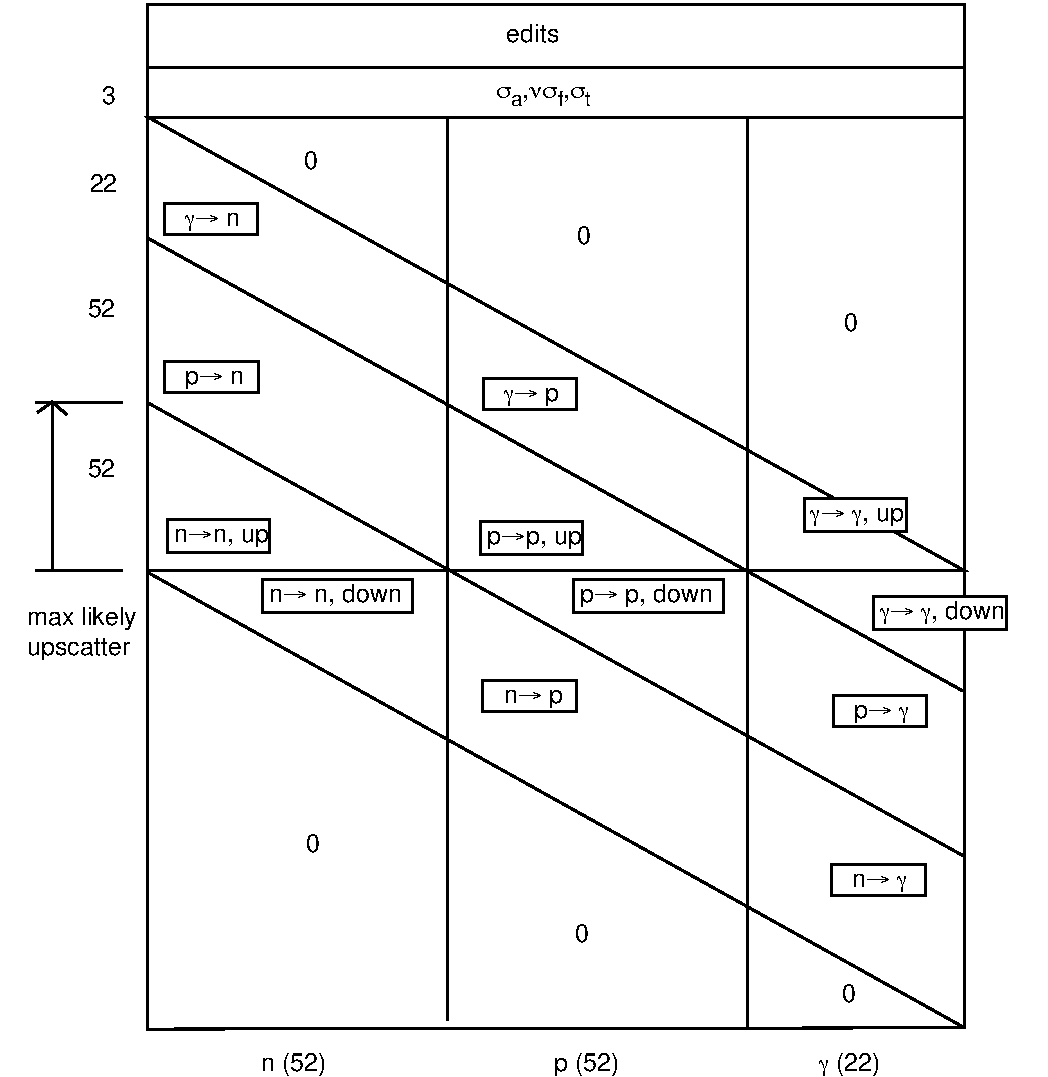
\includegraphics[keepaspectratio, height=5.5in, angle=0]{figs/groupr8}
\caption[Coupled neutron-proton-photon table]{Layout of a coupled table for
 the simultaneous transport of neutrons, protons, and gamma rays.  Normally,
 only the lower triangle of the ``p to n'' block would contain values for the
 upscatter portion of the table (the part above the line in the middle).  The
 ``group'' index increases from left to right, and the ``position'' index
 increases from top to bottom.}
\label{npg}
\end{figure}

There is a new ENDF format now becoming available that helps to
describe the production of all isotopes and isomers in a given system.
It uses a directory in File 8 to direct the code to productions
represented by MF=3, by MF=9 times MF=3, by MF=10, or by sections
of MF=6 times MF=3.  When this format is used, it is possible to
give the simple command

\small
\begin{ccode}

 10/

\end{ccode}
\normalsize

\noindent
to have production cross sections generated for every nuclide that
is produced.  These production sections are labeled with the ZA and
isomeric state of the products for use by subsequent NJOY modules.


\subsection{Coding Details}
\label{ssGROUPR_details}

The \cword{groupr}\index{groupr@{\ty groupr}} subroutine is exported
by the \cword{groupm}\index{modules!groupm@{\ty groupm}} module.
GROUPR begins by reading most of the user's input (see
\cword{ruinb})\index{ruinb@{\ty ruinb}}.  It then
locates the desired material and temperature on the input ENDF,
PENDF\index{PENDF}, and GENDF\index{GENDF} tapes, and reads in
the self-shielded unresolved cross sections (if any) from the PENDF
tape using \cword{stounr}\index{stounr@{\ty stounr}}.  If
self-shielding was requested, \cword{genflx}\index{genflx@{\ty genflx}}
is used to compute the weighting flux as described in
Section~\ref{ssGROUPR_WtFlux}.  The
next step is to write the header record for this material on the
output GENDF tape.

The code is now ready to begin the loop over reactions for this
material and temperature.  Either an input card is read to
get \cword{mfd}, \cword{mtd} and \cword{mtname} (the reaction name),
or the next reaction in
an automatic sequence is selected.  First, the default Legendre order,
secondary group count, and $\sigma_0$ count are selected for the reaction
in \cword{init}\index{init@{\ty init}}, and the retrieval routines are
initialized.  \cword{groupr} then processes the reaction using the
\cword{panel} logic described in
Section~\ref{ssGROUPR_GrpInt}.  If a ``shortcut'' fission
spectrum was requested (\cword{mfd=5}), for delayed fission, and
for the low-energy ``constant'' spectra, the spectrum is calculated
directly using \cword{getff}\index{getff@{\ty getff}}.  As the cross
sections for each group are obtained, they are printed out
(see \cword{displa}\index{displa@{\ty displa}}) and written to the
GENDF tape.  When the last group has been processed, \cword{groupr}
loops back to read a new input card for a new reaction.

This loop over reactions continues until a terminating ``\cword{0/}'' card is
read.  \cword{groupr} then proceeds to the next temperature, if any, and
repeats the loop over reactions.  After the last temperature has been
processed for the first material, an opportunity is provided to change
to a new material, keeping all the other input parameters unchanged.
A ``\cword{0/}'' card at this point causes all the files to be closed, prints
out the final messages, and terminates the \cword{groupr} run.

Automatic choice of the next reaction to be processed is done in one of
two ways.  For a simple range of MT numbers, such as the example 51 - 66
used above, the negative value is stored in the variable \cword{mtdp}
in the \cword{groupr} subroutine.  When \cword{mtdp} is negative,
\cword{mtd} is incremented after each reaction until it is greater than
the absolute value of \cword{mtdp}.  \cword{mtdp} is then reset to one,
and the code proceeds to the next input card.  When processing photon
data, \cword{mfd}=\cword{16}
will automatically change to \cword{17}, if necessary.  Similarly,
\cword{mfd}=21, 22, \ldots will automatically change to
\cword{mfd}=31, 32, \ldots.  A more automatic method is triggered by
\cword{mtd}=0.  In this case, a subroutine called
\cword{nextr}\index{nextr@{\ty nextr}} is called to return
the next value of \cword{mtd} to be used, and a subroutine called
\cword{namer}\index{namer@{\ty namer}} is called to generate the
reaction name.  For \cword{mfd}=3, \cword{nextr} finds the next
reaction in File 3 on the input PENDF tape.  MT=251-253 and
thermal data (MT=221-250) are excluded.  The MT values for the
special options (258, 259, {\it etc.}) do not appear on the PENDF
tape, and they must be requested explicitly.  For matrices,
GROUPR works with a set of lists loaded into global arrays by
\cword{conver}\index{conver@{\ty conver}}.  The list \cword{mf4}
contains all the neutron-scattering MT numbers that appear in the
File 4 part of the directory on the ENDF tape, and the list
\cword{mf6} contains all the MT numbers of sections of File 6 that
contain subsections that produce neutrons.  Therefore, reading
through these two lists returns all the neutron-producing matrix
reactions.  Similarly, the list \cword{mf12} contains all the
File 12 entries from the directory, \cword{mf13} contains the
File 13 entries, and \cword{mf18} contains all the MT
values for sections in File 6 that contain subsections for photon
production.  Scanning through these three lists produces all the
photon production matrix reactions.  Two arrays are used for
charged-particle producing reactions; the first index runs through
the charged particles in the order p, d, t, $^3$He, $\alpha$, recoil.
Taking proton production as an example, the list elements
\cword{mf6p(1,i)} contain the MT numbers of sections in File 6 that
contain subsections that produce protons.  The list elements
\cword{mf4r(1,i)} contain MT numbers from File 4 for two-body reactions
that produce protons; namely, MT600 - MT648.  \cword{nextr} scans through
both of these lists to return indexes to all the reactions that produce
protons.  The same procedure is used for the other charged particles.
The arrays \cword{mf10s} and \cword{mf10i} are used in a similar
way for nuclide production.

Subroutine \cword{namer}\index{namer@{\ty namer}} generates name
strings with up to 15 Hollerith words with 4 characters each
(60 characters).  The names depend on the ``ZA'' of the projectile
and the MT number for the reaction.  The parameter \cword{mfd}
is used to choose between the suffixes ``cross section'' and
``matrix''.   Some examples of the names produced follow:

\begin{center}
\begin{tabular}{lll}
   Name   &   Name   &   Name  \\ \hline
  \cword{(n,total)}   &  \cword{(n,heat)}  &  \cword{(p,p02)}  \\
  \cword{(n,elastic)} &  \cword{(n,p02)}   &  \cword{(p,n00)}  \\
  \cword{(n,2n)}      &  \cword{(p,elastic)}  &  \cword{(g,total)}  \\
  \cword{(n,n01)}     &  \cword{(p,2n)}    &  \cword{(g,pair)}  \\ \hline
\end{tabular}
\end{center}

Subroutines \cword{mfchk}\index{mfchk@{\ty mfchk}} and
\cword{mfchk2}\index{mfchk2@{\ty mfchk2}} are used with the
full input for reaction selection in GROUPR to check whether
\cword{mfd}=17 is needed when \cword{mfd}=16 was requested, or
whether one of the charged-particle File 4 values \cword{mfd}=31-36
is needed when \cword{mfd}=21-26 were requested.  The lists in
global variables like \cword{mf12} are used, just as for \cword{nextr}.

Subroutine \cword{gengpn}\index{gengpn@{\ty gengpn}} generates the
group bounds in the global array \cword{egn} for the neutron group
structure from input cards, from data statements, or by calculation.
Some of the data statements use energies in eV and some use lethargy.
Similarly, \cword{gengpg}\index{gengpg@{\ty gengpg}} generates the
photon group structure in global array \cword{egg} from input cards
or data statements; in this case, all bounds are in eV.

Subroutine \cword{genwtf}\index{genwtf@{\ty genwtf}} sets up the
weight function option requested with \cword{iwt} by reading the
input cards into \cword{weights}, transferring numbers from data
statements to \cword{weights}, or simply reporting the analytic
weight option requested.  Subroutine
\cword{getwtf}\index{getwtf@{\ty getwtf}} returns the values of the
weight function at energy $E$ by calculation or by interpolation
in the table established by \cword{genwtf}.  The current
version returns the same value for all Legendre orders.  Choosing
\cword{enext} is difficult for \cword{getwtf} because the functions have
not been explicitly linearized.  It is important to generate extra grid
points in energy regions where the weight function may vary faster than the
cross section (for example, in the fusion peak).

Subroutine \cword{genflx}\index{genflx@{\ty genflx}} computes the
self-shielded weighting flux using either the Bondarenko model
or the flux calculator, and it writes the result on a scratch tape
using the \cword{loada} utility routine.  When fluxes are needed
for the generalized group integrals, they are read from this
scratch file using \cword{finda}\index{finda@{\ty finda}} (see
\cword{getflx}).  Subroutine \cword{genflx} starts by checking for
the weighting option.  If the Bondarenko model was selected, it
initializes \cword{gety1}\index{gety1@{\ty gety1}} and
\cword{getwtf}\index{getwtf@{\ty getwtf}} to read the total
cross section from the PENDF tape and the smooth weighting function
$C(E)$ set up by \cword{genwtf}\index{genwtf@{\ty genwtf}}.  It then
steps through the union grid of $\sigma_t(E)$ and $C(E)$ computing
the flux vs. $\sigma_0$ and Legendre order by means of Eq.~\ref{Eq14}.
In the unresolved energy range, \cword{getunr}\index{getunr@{\ty getunr}}
is used to retrieve the unresolved cross sections as a function
of $\sigma_0$, and Eq.~\ref{Eq22} is used to compute the weighting
flux.  In both cases, the data at each energy are stored as the
1+(\cword{lord}+1)*\cword{nsigz} components

\vspace{6 pt}
\cword{  e, phi(il,iz)},
\vspace{6 pt}

\noindent where \cword{il} runs from 1 to \cword{lord}+1 and
\cword{iz} runs from 1 to \cword{nsigz}.

If the flux calculator option was requested,
\cword{genflx}\index{genflx@{\ty genflx}} sets up the
parameters for the calculation and requests needed storage space.  Next,
the cross section retrieval routines \cword{gety1} and \cword{gety2} are
set up to return total and elastic cross sections from the PENDF tape.
A lower energy limit, \cword{felo}, is chosen, and the cross
sections are read into storage until a maximum energy, \cword{fehi}, or a
maximum number of points, \cword{nemax}, is reached.

The slowing-down equation, either Eq.~\ref{Eq33} or Eq.~\ref{Eq37},
is then solved from the break energy down to \cword{felo}.  The
scattering source from energies above the break is based on the
NR approximation\index{narrow resonance approximation}.  When the
calculation is finished, fluxes from $10^{-5}$ eV to \cword{felo} are
written to the scratch file using \cword{loada} in the same format used
for the Bondarenko option.  From \cword{felo} to the energy break point,
fluxes are transferred from memory to the \cword{loada} file.  Finally,
above the break point, fluxes are computed and saved using the
Bondarenko model.

Subroutine \cword{init}\index{init@{\ty init}} is used to set up
the number of $\sigma_0$ values, secondary energy groups, and
Legendre components for each combination of \cword{mfd} and
\cword{mtd}. If \cword{mfd}=8, a special copy of File 6 is
made for use in \cword{getaed}\index{getaed@{\ty getaed}}.  The
list of reactions to be self-shielded can be changed if desired.
The number of secondary groups \cword{ng} helps determine the
storage required for the accumulating group integrals (see
allocatable array \cword{ans}) in \cword{groupr}.  For simple
cross section vectors, \cword{ng}=2.  The \cword{nz}*\cword{nl} flux
components are stored first, followed by the \cword{nz}*\cword{nl} cross
section components.  When all the panels for one group have been
processed, dividing position 2 by position 1 gives
the group-averaged cross section.  For ratio quantities like
$\overline\nu$ and $\overline\mu$ (\cword{mtd}=251-253, 452, 455, 456),
\cword{ng} is 3.  Once again, the flux components are stored first,
followed by the \cword{nl}*\cword{nz} components of \cword{ratio}*\cword{sigma},
followed by the components of the cross section.  This arrangement
allows for the calculation of group-averaged values
of \cword{ratio}*\cword{sigma},
\cword{ratio}, or cross section by dividing position 2 by 1, position
2 by 3, or position 3 by 1, respectively.  For matrices, \cword{ng} is
set to one more than the number of secondary groups (\cword{ngn} or
\cword{ngg}).  The \cword{nl}*\cword{nz} flux components are stored first,
followed by the \cword{nl}*\cword{nz} integrals for each secondary-energy group
in turn.

Subroutine \cword{panel}\index{panel@{\ty panel}} performs the
generalized group integrals using the logic described in
Section~\ref{ssGROUPR_GrpInt}.
For most calls to \cword{panel}, the lower point of each ``panel''
was computed as the upper point of the previous panel.  Therefore,
\cword{panel} is careful to save these previous values.  However,
if the bottom of the panel is just above a discontinuity, new values
of cross section and flux are retrieved.  Once the values at the
lower boundary of the panel are in place, new values for the
top of the panel are retrieved (see \cword{flux}, \cword{sig}).
If the top of the panel is at a discontinuity in $\sigma$ or at a group
boundary, the energy used is just below the nominal top of the panel.
``Just below'' and ``just above'' are determined by \cword{rndoff} and
\cword{delta}.  For maximum accuracy, these numbers should be chosen such
that \cword{rndoff}$>$1, \cword{delta}$<$1, and
\cword{rndoff}*\cword{delta}$<$1 for the
precision of the machine being used.

For simple average cross sections, the integrals of $\sigma{\times}\phi$ and
$\phi$ are computed for the panel using trapezoids.  This is justified by
the linearization of $\sigma$; the value of $\sigma{\times}\phi$ at the
midpoint is too uncertain to justify a more complex treatment.  For
two-body scattering, the feed function is far from linear over the panel.
In fact, it can show oscillations as described in
Section~\ref{ssGROUPR_TwoBody}.  The
integral of the triple product ${\cal F}{\times}\sigma{\times}\phi$ is
obtained by Lobatto quadrature\index{Lobatto quadrature} of order 6 or 10
using the quadrature points and weights given in the parameter statements
(see \cword{qp6}, \cword{qw6}, \cword{qp10}, \cword{qw10}).  The
cross section and reaction rate are determined at each quadrature point
by interpolation, and the feed function is obtained by \cword{getff}.
For many reactions, \cword{ff} will be nonzero for only a certain range
of secondary groups.  The value \cword{ig1} is the index to the first
nonzero result, and \cword{ng1} is the number of nonzero values of
\cword{ff} in the range.  Subroutine \cword{panel} maintains the two
corresponding values \cword{iglo} and \cword{ng} to specify the
nonzero range of values in array \cword{ans}.  Finally, the flux
and cross section at the top of the panel are transferred to
\cword{flst} and \cword{slst}, and control is returned
to the panel loop in \cword{groupr}.

Subroutine \cword{displa}\index{displa@{\ty displa}} is used to
print cross sections and group-to-group matrices on the output
listing (\cword{nsyso}).  Small values are removed for efficiency.
Note that different formats are used in different
circumstances.  Infinitely dilute data are printed without $\sigma_0$
labels.  Isotropic matrices are printed with several final groups on each
line.  Delayed neutron spectra are printed using the Legendre order
variable for time groups and with the time constants given on a heading line.

Subroutine \cword{getflx}\index{getflx@{\ty getflx}} returns
\cword{nl}*\cword{nz} components of the weighting flux.  If
\cword{nsigz} is 1, the flux is computed using
\cword{getwtf}\index{getwtf@{\ty getwtf}}, and all Legendre orders
are taken to be equal.  When self-shielding has been requested, the
flux components are obtained by interpolating between adjacent values
retrieved with \cword{finda} from the scratch tape written by
\cword{genflx}.  The grid energies found on the scratch tape are used
to get \cword{enext}.  The flux is taken to be
continuous, so \cword{idis} is always set to zero.

Subroutine \cword{getyld}\index{getyld@{\ty getyld}} returns the yield
needed by \cword{getff} for fission (MT=452, 455, or 456 from File 1)
or radionuclide production yields from File 9 (using \cword{mfd}=3zzzaaam).
 This routine also retrieves the delayed neutron time constants when
\cword{mtd}=455.  Tabulated yields are obtained by interpolation
using the utility routine \cword{terpa}\index{terpa@{\ty terpa}}.
Polynomial data are expanded by direct computation.

Subroutine \cword{getsig}\index{getsig@{\ty getsig}} returns
\cword{nl}*\cword{nz} components of the cross section using point data
from the PENDF tape and self-shielded unresolved data, if present,
from \cword{getunr}\index{getunr@{\ty getunr}}.  The routine starts by
adjusting MF and MT for the special options (\cword{mtd}=258-259,
\cword{mfd}=3zzzaaam, {\it etc.}) and locating the desired section on
the PENDF tape.  Subroutine \cword{getsig} is then called for each
desired energy value $E$ in increasing order.  For \cword{mtd}=258 or 259,
the appropriate velocity or lethargy is computed from $E$ and returned.
In the more general cases, \cword{gety1} is used to retrieve the pointwise
cross section from the PENDF tape, and \cword{getunr} is called to replace
this value with self-shielded unresolved cross sections if necessary.

The unresolved cross sections are handled using
\cword{stounr}\index{stounr@{\ty stounr}}
and \cword{getunr}\index{getunr@{\ty getunr}}.
Subroutine \cword{stounr} locates the desired material
and temperature in MF=2, MT=152 of the PENDF tape, and then it copies
the data into the global allocatable storage array \cword{unr}.  The
$\sigma_0$ grid on the PENDF tape does not have to agree with the list
requested for \cword{groupr}, but a diagnostic message will be printed
if they are different.  However, the \cword{ntemp} values of temperature
requested by \cword{groupr} must agree with the first \cword{ntemp}
temperatures on the PENDF tape, or a fatal error will result.
Subroutine \cword{getunr} checks whether $E$ is in the unresolved energy
range and whether MT is one of the resonance reactions.  If so,
it locates the desired interpolation range in the \cword{unr} array, and
interpolates for the self-shielded cross sections.  If this is an
energy range where resolved and unresolved ranges overlap, the
resolved part is added to the background $\sigma_0$ before interpolation.
The subroutine \cword{terpu} is used for interpolating in the unresolved
cross section tables.  The special value MT=261 is used to select
the $\ell{=}1$ component of the total cross section.  Note that
\cword{getsig} also uses this $\ell{=}1$ value for $\ell{=}2, 3, \ldots\,$.

Subroutine \cword{getff}\index{getff@{\ty getff}} returns the
feed function \cword{ff} using different portions of the coding
for different options.  The first section is used for cross sections
and ratio quantities.  The same yield \cword{yld}
is returned for every $\ell$-component in \cword{ff}.

The second section of \cword{getff} is for neutron continuum transfer
matrices.  The yield is either determined from MT [for example,
\cword{yld}=2 for MT=16, the (n,2n) reaction], or it is obtained using
\cword{getyld}\index{getyld@{\ty getyld}} for fission.  Next, the
angular distribution is obtained using
\cword{getfle}\index{getfle@{\ty getfle}} (see $F$ in Eq.~\ref{Eq83}),
and the secondary energy distribution is obtained using
\cword{getsed}\index{getsed@{\ty getsed}} (see $g$ in
Eq.~\ref{Eq83}).  Finally, the product of the three factors is loaded
in \cword{ff}.  Note that the range of groups returned extends from
\cword{iglo}=1 to the highest nonzero result, for a total of \cword{ng}
groups.  Since \cword{ff} for these reactions is a smooth function of
incident energy, \cword{nq} is set to zero, and no additional quadrature
points will be used in \cword{panel}\index{panel@{\ty panel}}.

The third section of \cword{getff} is for gamma production matrices.  The
photon yields are obtained using \cword{getyld}\index{getyld@{\ty getyld}}.
In general, there are \cword{nyl} different yields, each one corresponding
to a different discrete gamma ray, or to the continuum.  The angular
distributions for these gamma rays are obtained using
\cword{getgfl}\index{getgfl@{\ty getgfl}} (most ENDF/B photons
are given as isotropic).  The energy distribution for the continuum
(if any) is obtained by \cword{getsed}\index{getsed@{\ty getsed}}.
Now, the code loops through the photon group structure placing each
discrete photon in the appropriate group and adding in the continuum
part.  During this loop, the range of nonzero values (\cword{iglo},
\cword{ighi}) is determined.  Finally, the nonzero values are packed
into \cword{ff}, and \cword{iglo} and \cword{ng} are returned to
describe the distribution.  Again, \cword{nq}=0 is used.

The fourth section of \cword{getff} handles two-body scattering, either
elastic or discrete-level inelastic, and both neutrons and charged
particles.  First, subroutine \cword{parts}\index{parts@{\ty parts}}
is called to set up the particle type, $A'$ value, and the scattering
law for reactions that use File 4.  Then
\cword{getdis}\index{getdis@{\ty getdis}} is called
to finish the processing.

The fifth section handles thermal-neutron scattering.  The bulk of the
work is done by \cword{getaed}\index{getaed@{\ty getaed}}, which is
discussed below.  Subroutine \cword{getff} takes the output of
\cword{getaed} and packs it into the final result, \cword{ff}.

The last two sections of \cword{getff} are used to process energy-angle
distributions from ENDF-6 format sections of File 6.  The subroutine
simply calls \cword{getmf6}\index{getmf6@{\ty getmf6}}.

Subroutine \cword{parts}\index{parts@{\ty parts}} is used to set
up particles for reactions that use File 4.  Different branches are
used for ENDF-6 and earlier ENDF versions because the MT numbers
used for charged-particle discrete levels have been changed.  For
example, proton levels use MT=600-649 in ENDF-6 libraries, but
MT=700-719 in earlier libraries.  If \cword{mfd}=3, no action
is taken.  For other \cword{mfd} values, the routine determines
\cword{zap}, \cword{aprime}, and \cword{law}.  The
result depends on whether File 4 or File 6 data are to be used.

Subroutine \cword{getmf6}\index{getmf6@{\ty getmf6}} is used
to compute the feed function for reactions represented in File 6.
As is common with NJOY subroutines, it is called with \cword{ed}=0
to initialize the subroutine.  The first step is to locate the
desired section of File 6 on the input ENDF tape.  It then sets
the parameter \cword{zad} (for ZA desired) based on the input
value \cword{mfd} and searches through the section for the
desired subsection.  If this subsection has \cword{law}=4, it
defines a recoil particle; the code backs up to the first
subsection in the section, which is assumed to be the subsection
describing the emitted particle.  The subroutine has now arrived at
statement number 140, where it decides whether to branch to special
coding for two-body reactions (statement number 500) or phase-space
reactions (statement number 150).  All the other options have a TAB2
record at this point that defines the incident energy grid.  For
\cword{law}=1, the data for the first incident energy are read in
and converted to the Lab frame by \cword{cm2lab}.  Similarly, for
\cword{law}=7, the data are read in and converted to a \cword{law}=1
format by \cword{ll2lab}\index{ll2lab@{\ty ll2lab}}.

For a normal entry, \cword{getmf6} interpolates for the particle yield
for the current particle.  For all of the laws except 2-5 (discrete
two-body laws), it then checks to see whether the energy \cword{ed} is
in the current panel (or if this is the first time in the first panel).
If not, it moves the high data to the low position and reads in new
high data.  Of course, it also converts the new high data to the correct
form with \cword{cm2lab}\index{cm2lab@{\ty cm2lab}} or
\cword{ll2lab}\index{ll2lab@{\ty ll2lab}}.  Once \cword{ed} is in the
current panel, the code reaches statement number 300, which sets up the
loop over secondary energy by initializing
\cword{f6lab}\index{f6lab@{\ty f6lab}}.  This loop
uses a grid that consists of the \cword{epnext} values returned by
\cword{f6lab} and the group bounds \cword{eg(i)}.  The actual integral
over $E'_L$ inside each group uses trapezoidal integration.  The last
step for laws 1, 6, and 7 is to add in the contributions to the feed
function from discrete energies in File 6.  For the discrete two-body
laws (2-5), the routine goes through statement number 500, which
simply calls \cword{getdis}.  For all laws, the last step is to check
the normalization of the feed function.  If the error is large, a
message is printed out.  In any case, the results are adjusted to
preserve exact normalization.

Subroutine \cword{cm2lab}\index{cm2lab@{\ty cm2lab}} is used to convert
a CM distribution starting at \cword{inow} in \cword{cnow} into a
Lab distribution, which will be stored starting at \cword{jnow}.  This
routine generates a grid for the
Lab secondary energy $E'_L$ by adaptive reconstruction.  The
reconstruction stack is first primed with
$p_{L\ell}(E,0)$ as computed by \cword{f6cm} and
$p_{L\ell}(E,E'_{\rm next})$ (also from \cword{f6cm}), where
the value $E'_{\rm next}$ is the value \cword{epnext} returned by the
first call to \cword{f6cm}.  This panel is then divided in half, and
the value returned by \cword{f6cm} is compared with the linear
interpolate.  If they agree within 0.5\% (see \cword{tol}), this panel
is converged.  Otherwise, it is subdivided further.  When convergence
has been achieved for this panel, a new panel is chosen, and it is
subdivided to convergence.  When the entire range for $E'_L$ has been
processed, the final parameters are loaded into the new File 6 record
for $p_{L\ell}(E,E'_L)$ (which starts at \cword{jnow} in \cword{cnow}),
and the routine returns to \cword{getmf6}.

Subroutine \cword{f6cm}\index{f6cm@{\ty f6cm}} is used to compute
the Legendre coefficients of the double-differential scattering
function $p_\ell(E{\rightarrow}E')$ in the Lab system from
data given in File 6 in the CM frame.  The memory area
\cword{cnow} contains the raw data.  It is necessary to call the
routine \cword{ep}=0 for each new value of $E$.  Thereafter, values
of \cword{ep} can be requested in any order.  This is required by the
adaptive scheme used to generate the Lab $E'$ grid in \cword{cm2lab}.
The conversion uses Eqs.~\ref{yy1} - \ref{yy6}.  On a normal entry
with $E'_L{>}0$, the code computes the lower limit of the integral
$\mu_{\rm min}$.  It then sets up an adaptive integration over a panel
starting at $\mu{=}1$. The value for $E'_C$ is computed using

\begin{equation}
   E'_C=(1+c^2-2c\mu_L)E'_L \,\,,
\end{equation}

\noindent
which is based on Eq.~\ref{yy2}, and either
\cword{f6ddx}\index{f6ddx@{\ty f6ddx}} or
\cword{f6psp}\index{f6psp@{\ty f6psp}} is called to compute
$p_C(E,E'_C,\mu_C)$ and \cword{epnext}.  The lower limit of
the integration panel is then computed by setting
$E'_C$ equal to \cword{epnext} and solving for the CM cosine using

\begin{equation}
   \mu_C=\frac{\mu_L-c}{\sqrt{1+c^2-2c\mu_L}} \,\,.
\end{equation}

\noindent
Of course, the larger of this result and $\mu_{\rm min}$ is used as
the lower bound of the panel.  Therefore, the adaptive integration operates
on a nice continuous function.  It continues subdividing the $\mu_C$ grid
in this panel until convergence is achieved within 0.5\% for all
Legendre orders.  The lower bound of this panel
becomes the upper bound of a new panel, and a new lower bound is selected
as above.  The integration is carried out over successive panels until
$\mu_{\rm min}$ is reached.  When the calculation of the continuum part
of $p_{L\ell}$ is finished for these values of $E$ and $E'_L$, the
routine checks for possible contributions from delta functions.  Next,
the routine scans through the computed coefficients and zeros out any small
ones that may just be noise.  Finally, it chooses a value for
\cword{epnext} and returns.

Function \cword{f6ddx}\index{f6ddx@{\ty f6ddx}} is used to compute
the double-differential scattering function $f(E{\rightarrow}E',\omega)$,
where secondary energy $E'$ and scattering cosine $\omega$ are in the
CM system.  On entry, \cword{cnow} contains the File 6 data for
a particular value of $E$, and \cword{f6ddx} must be called once
with \cword{ep}=0 for each new value of $E$.  Thereafter,
\cword{ep} values can be requested in any order (this is
required by the adaptive scheme used to convert to the Lab system in
\cword{f6cm}).  For a normal entry with \cword{ep}$>$0, the code searches
for the panel in the data that contain the requested value of $E'$.
If \cword{lang}=1 for this subsection of File 6, the data are already
given as Legendre coefficients, and the code simply interpolates for the
desired results.  If \cword{lang}=2, the data use the Kalbach-Mann scheme
for representing the energy-angle distribution.  This routine includes
both the original Kalbach-Mann representation\cite{km} and the newer
Kalbach representation\cite{k86}.  It has been set to use the latter
by the parameter statement \cword{k86}=1.  The code interpolates for
the model parameters at $E'$ and computes the desired answer with the
model's formulas.  The ENDF-6 format also allows CM distributions given
as values tabulated versus scattering cosine (see \cword{lang}=11-15).
Note that there is a ``stub'' to take special action at low energies.
It is currently disabled by the statement \cword{efirst}=0.0, but it may
be used sometime in the future to account for the fact that the
low-energy dependence of the scattering function must vary as
$f(E')=c*\sqrt{E'}$.

Function \cword{bach}\index{bach@{\ty bach}}
computes the Kalbach-86 $a$ parameter, which depends
on the neutron separation energy for the target \cword{izat} using the
liquid-drop model without pairing and shell terms.  The formula
used describes the reaction $a+B\rightarrow C+d$:

\begin{eqnarray}
   E_{sep} & = & 15.68\bigl(A_C-A_B\bigr) \nonumber\\
           & - & 28.07\bigl(\frac{(N_C-Z_C)^2}{A_C}
                 -\frac{(N_B-Z_B)^2}{A_B}\bigr) \nonumber\\
           & - & 18.56\bigl(A_C^{2/3}-A_B^{2/3}\bigr) \nonumber\\
           & + & 33.22\bigl(\frac{(N_C-Z_C)^2}{A_C^{4/3}}
                 -\frac{(N_B-Z_B)^2}{A_B^{4/3}}\bigr) \nonumber\\
           & - & 0.717\bigl(\frac{Z_C^2}{A_C^{1/3}}
                 -\frac{Z_B^2}{A_B^{1/3}}\bigr) \nonumber\\
           & + & 1.211\bigl(\frac{Z_C^2}{A_C}
                 -\frac{Z_B^2}{A_B}\bigr) \,\,,
\end{eqnarray}

\noindent
where $A$ stands for atomic weight, $Z$ for charge number, and
$N$ for neutron number.  Note that, even for reactions like (n,2n),
$C$ is the residual nucleus resulting from the removal of
\underline{one} particle, $d$; it is not necessarily the real
physical residual nucleus for the reaction.  If the target \cword{izat}
is an element, $E_{sep}$ has to be computed for some dominant isotope
in the element.  Dominant isotopes are assigned in this routine for
some materials that often appear as elements in ENDF evaluations; if
the particular target required does not appear, a fatal error message
is issued.  The user will have to add a line to the routine for the
material and reassemble the code.

Subroutine \cword{ll2lab}\index{ll2lab@{\ty ll2lab}} converts File 6
from Law-7 format to Law-1 format using the laboratory Legendre
representation.  Law 7 represents the double-differential scattering
distribution $f(E{\rightarrow}E',\mu)$ by giving a series of tables of
$f(E{\rightarrow}E')$ for series of $\mu$ values.  On entry, the entire
Law-7 section is stored in \cword{c} starting at \cword{inow}.  The code
loops through a set of $E'$ values chosen to be the union of all the
$E'$ grids for all the different $\mu$ values.  For each point on this
union grid, the code interpolates for all the corresponding $f(\mu)$
values, and it uses them to compute \cword{nl} Legendre coefficients
$f_\ell(E')$.  After completing the calculation for a new value of $E'$,
it checks the normalization of the result, and then it checks back to see
whether the previous value is still needed to represent the curves
$f_\ell(E')$ within a tolerance of 0.5\%.
The results are written in \cword{c} starting at \cword{jnow}.  They
have the Law-1 Legendre form, namely, sets of values $E'$, $f_0(E')$,
$f_1(E')$, \ldots, $f_{{\rm NL}-1}(E')$, given for a series of $E'$
values starting with zero.

Subroutine \cword{f6lab}\index{f6lab@{\ty f6lab}}
is used to return the Legendre coefficients of the
double-differential scattering function $f_\ell(E{\rightarrow}E')$
for particular values of $E$ and $E'$ in the Lab system (see \cword{e}
and \cword{ep}) from a part of File 6 in Law-1 format.  Since Law-7
sections have been converted to Law-1 format using \cword{ll2lab}, and
since CM sections in Law-1 format have been converted to the Lab frame
using \cword{cm2lab}, the only two roles left for this subroutine are
interpolation to the desired values of $E$ and $E'$ and preparation
of Legendre coefficients for sections that use the File-6 variant with
\cword{law}=1 and \cword{lang}=11-15 (laboratory distributions tabulated)
vs. $\mu$.  Only the continuum portion of the distribution is processed
here; any delta functions given in File 6 must be handled separately.
The routine is initialized by calling it with \cword{ep}=0.  Data
for the two incident energy values that bracket $E$ are already present
in \cword{clo} and \cword{chi}.  Then the routine extracts
various parameters from the \cword{c} array and prepares the variables
used to control interpolation.  These variables are complicated, because
this routine handles three different interpolation schemes: ``cartesian'',
``unit base'', and ``corresponding point'' (see the ENDF-6
manual\cite{ENDF102} for more details).  For a normal entry, the code searches
the data in \cword{clo} and \cword{chi} for the intervals containing $E'$.
If \cword{lang}=1, it performs a two-dimensional interpolation for the
\cword{nl} coefficients at $E$ and $E'$.  For \cword{lang}$>$1, it computes
the Legendre coefficients from the File 6 data, and then
does the two-dimensional interpolation.  Finally, it computes
\cword{epnext} and returns.

Subroutine \cword{getdis}\index{getdis@{\ty getdis}} is used
to compute the feed function for elastic or discrete inelastic
scattering of neutrons or charged particles using either File 4
or File 6 data.  First, the angular distribution is retrieved
with \cword{getfle}, and an appropriate quadrature order is
selected using Eq.~\ref{Eq77}.  Then, a group loop from low energy to
high energy is used to compute the $\omega_1$ and $\omega_2$ limits of
Eq.~\ref{Eq75}, and the range ($\omega_1,\omega_2$) is subdivided using
the appropriate Gauss-Legendre quadrature points (see \cword{qp4},
\cword{qp8}, \cword{qp12}, and \cword{qp20}).  The function $f(E,\omega)$
is computed at each of these quadrature points using Eq.~\ref{Eq76}
and the angular distribution previously returned by
\cword{getfle}\index{getfle@{\ty getfle}}.  The laboratory cosine
at the quadrature point, $\mu\bigl[\omega\bigr]$, is computed
using Eq.~\ref{Eq72}.  Finally, the integrand of Eq.~\ref{Eq75}
is multiplied by the appropriate quadrature weight (\cword{qw4},
\cword{qw8}, \cword{qw12}, or \cword{qw20}) and added into the
accumulating integral.  This continues until $\omega_2=1$.
The nonzero values of \cword{ff} and the parameters \cword{iglo}
and \cword{ng} are then complete for this value of $E$.

The next step is to determine \cword{enext} based on the next critical
point as given by Eqs.~\ref{Eq79} - \ref{Eq82}.  Special cases are used
for elastic scattering to avoid numerical problems.  Note that the
discontinuity flag \cword{idisc} is set for critical points.  The
\cword{nq} variable is also set to force \cword{panel} to subdivide the
initial-energy integration.

Subroutine \cword{getfle}\index{getfle@{\ty getfle}}
retrieves or computes the Legendre coefficients
for the angular distribution of a reaction at incident energy E.  When
called with \cword{e}=0, \cword{getfle}\index{getfle@{\ty getfle}}
requests storage for the raw data, reads in the File 4 information
for the first two incident energies on the file, and then
uses \cword{getco} to retrieve the corresponding
coefficients.  On subsequent entries with \cword{e}$>$0, \cword{getfle}
simply interpolates for the desired coefficients.  When \cword{e} exceeds
the upper energy in storage, the values for the upper energy are moved
to the lower positions, and new upper values are read and converted to
coefficients.  An isotropic distribution is returned if \cword{e} is
outside the range of the angular data from File 4.

Subroutine \cword{getaed}\index{getaed@{\ty getaed}}
retrieves angle-energy data for thermal scattering
reactions.  For coherent elastic scattering, the routine reads through the
cross section on the PENDF tape using \cword{gety1} and locates the Bragg
edges.  On each subsequent call to \cword{getaed}, the Legendre components
of the cross section are computed using Eq.~\ref{Eq67}.  For incoherent
elastic scattering, the routine is first initialized by reading in the
raw data for the first energy.  On subsequent entries, a test is made
to see whether \cword{e} is in the range \cword{elo} to \cword{ehi}.
If not, the high data are moved to the low positions, and new high data are
read.  The Legendre components are then computed using Eq.~\ref{Eq69}.  For
incoherent inelastic scattering, \cword{getaed} is initialized by reading
in the raw data for the first two incident energies. On subsequent entries,
the subroutine checks to see whether \cword{e} is between \cword{elo} and
\cword{ehi}.  If not, the data for \cword{ehi} are moved to the low
positions, and new raw data are read from File 6 and binned.  Once the
correct data are in place, the desired energy-angle distribution is computed
by using a combination of interpolation along lines of constant energy
transfer and unit-base interpolation.

Subroutine \cword{getgfl}\index{getgfl@{\ty getgfl}}
returns the Legendre coefficients for the angular
distributions for all discrete and continuum photons for a reaction
simultaneously.  When called with \cword{ed}=0, the routine reads File 14
into scratch storage and finds the starting location for the subsection
describing each photon.  On subsequent entries with \cword{ed}$>$0,
\cword{getgfl} sets up a loop over the \cword{ng} photons on this section
of File 14.  For each photon, it searches for the energy panel that
contains \cword{ed}, uses \cword{getco}\index{getco@{\ty getco}} to retrieve
or compute the Legendre coefficients at the upper and lower File 14
energies, and interpolates for the desired coefficients at \cword{ed}
using \cword{terp1}.  Since most ENDF photons are represented as
isotropic, a special short-cut calculation is provided for that
case.  Isotropic results are also returned if \cword{ed} is outside
the range of the data in File 14.

Subroutine \cword{getco}\index{getco@{\ty getco}}
is used by both \cword{getfle}\index{getfle@{\ty getfle}} and
\cword{getgfl}\index{getgfl@{\ty getgfl}} to retrieve or compute
Legendre coefficients from data in File 4 or File 14 format.
The user can request output in either the Lab or CM system, and
the raw data can be either Legendre coefficients
or tabulated probability versus emission cosine.  However, if the raw data
are in the laboratory system, CM coefficients cannot be produced.  If
the raw data are already in the form of coefficients in the desired system,
\cword{getco} simply checks for the maximum Legendre order needed using
a tolerance of \cword{toler}=1e-6 and returns the coefficients in
\cword{fl} and the order in \cword{nl}.  If coordinate conversion is
required, or if the raw data are tabulated, \cword{getco} sets up the
integral over cosine using Gauss-Legendre quadrature of order 20 (see
\cword{qp} and \cword{qw}).  The scattering probability for the quadrature
point is computed from the coefficients or obtained by interpolating in
the tabulation.  The Legendre polynomials in the desired reference system
are then computed.  If the raw data are in the CM system ($\omega$) and the
result is to be in the Lab system ($\mu$), the desired polynomials
are $P_{\ell}(\mu\bigl[\omega\bigr])$;  otherwise, the quadrature angle
is used directly to compute the polynomials.  Once the coefficients have
been computed, they are checked using \cword{toler} to determine the
maximum order, \cword{nl}, and the results are returned
in \cword{fl}.

Subroutine \cword{getgyl}\index{getgyl@{\ty getgyl}}
is used to retrieve the yields for all photons
emitted in a specified reaction simultaneously.  The raw data are
obtained from the ENDF/B tape as either yields (MF=12) or production
cross section (MF=13).  In the latter case, \cword{getgyl} actually
returns the fraction of the total yield assigned to each photon.  The
cross section returned by \cword{getsig}\index{getsig@{\ty getsig}}
is the total photon production cross section from MF=13 on the
PENDF tape, which makes the resulting integral correct.  Using
the normal GROUPR procedure, \cword{getgyl}\index{getgyl@{\ty getgyl}}
is initialized by calling it with \cword{ed}=0.  The entire
File 12 or File 13 is read into scratch storage, and the
starting location for each subsection is determined.  On subsequent entries
(\cword{ed}$>$0), the routine loops over the \cword{nyl} photons found, and
uses \cword{terpa} to compute the yield at \cword{ed}.  If this is a
primary photon, a discontinuity is set up at the energy where the photon
will change groups.  For MF=12, the calculation is finished.  For MF=13,
the numbers calculated above are converted to fractions of the total yield
by dividing by the total production subsection from File 13.  This routine
does not handle ENDF/B transition probability arrays directly, because
they will have been converted to File 12 yields by
\cword{conver}\index{conver@{\ty conver}}.

Subroutine \cword{conver}\index{conver@{\ty conver}}
converts ENDF/B evaluations to a standard form.  If transition
probability arrays were used in File 12, they are converted
to yields and written back into File 12.  If a section with MF=1 and
MT=456 is missing from the evaluation, a copy of MT=452 is added to the
tape as MT=456.  In addition, a second copy of the modified tape is made
on unit \cword{nscr}.  While \cword{conver} is reading through the tape,
lists of the reactions in File 4, File 12, and File 13 are written to
to global arrays for use by the automatic reaction selection logic in
\cword{nextr}.  For ENDF-6 evaluations containing File 6, the routine
scans through File 6 looking for sections that produce neutrons, photons,
or charged particles.  The MT numbers for these sections are stored into
\cword{mf6}, \cword{mf18}, and \cword{mf6p}.  The routine also checks
for sections of File 4 containing charged-particle angular distributions
and records their MT numbers in \cword{mf4r}.  Finally, if the section
MF=6/MT=2 contains charged-particle elastic scattering information given
using the nuclear-plus-interference format, it is converted into the
residual-cross-section format for \cword{getdis}.

Subroutine \cword{getsed}\index{getsed@{\ty getsed}}
returns the secondary-energy distribution for
neutrons or continuum photons for all groups simultaneously.  Both
tabulated and analytic functions are handled.  \cword{getsed} is
initialized for a particular reaction by calling it with \cword{ed}=0.
First, scratch storage is allocated, and all the  subsections are read in.
Analytic subsections are left in their raw form, but tabulated subsections
are averaged over outgoing energy groups for each of the given incident
energies.  The array \cword{loc} contains pointers for each subsection.
On subsequent entries (\cword{ed}$>$0), \cword{getsed} loops over the
subsections for this reaction.  It first retrieves the fractional
probability for the subsection using \cword{terpa}\index{terpa@{\ty terpa}}.
If an analytic law is specified, \cword{anased}\index{anased@{\ty anased}}
is used to compute the group integral for each secondary-energy
group.  Each integral is multiplied by the fractional probability
for the law and accumulated into \cword{sed}.  For tabulated data,
the routine simply interpolates between the two values for the
group integrals using \cword{terp1}, and accumulates them
into \cword{sed}.  Note that various restrictions on the ordering of
subsections and prohibition of multiple tabulated subsections needed
for earlier versions of GROUPR are no longer required.  Upscatter
is not allowed in secondary-energy distributions except for fission
or photon production.  If found, it is put into the ``in-group''
($g'{=}g$).

Subroutine \cword{anased}\index{anased@{\ty anased}}
is used to calculate the integral from
\cword{e1} to \cword{e2} for one of the analytic laws (see
Eqs.~\ref{Eq86} - \ref{Eq115}).  The routine uses the SLATEC version
of the reduced complementary error function from the NJOY2016
math module.  The resulting integral is returned
in \cword{g}.

Subroutine \cword{hnab}\index{hnab@{\ty hnab}} is used to compute
the special functions required for analytic law 11, the energy-dependent
Watt spectrum.  The method used is described in the
\hyperlink{sBROADRhy}{BROADR}\index{BROADR}
chapter of this manual.


\subsection{Error Messages}
\label{ssGROUPR_msg}

The fatal error messages and warning messages from GROUPR
are listed below, along with recommended actions to recover
from the problem.

\begin{description}
\begin{singlespace}

\item[\cword{error in groupr***unable to find mat=---, t=---.}] ~\par
  Check for input error or wrong PENDF tape mounted.

\item[\cword{error in groupr***photons not allowed with igg=0.}] ~\par
  In order to produce photon data, a photon group structure
  must be requested.  Check the input on card 2.

\item[\cword{error in groupr***illegal mfd.}] ~\par
  Check input \cword{mfd}; legal values are 3, 5, 6, 8, 12, 13, 16, 17,
  18, 21-26, 31-36, and the isotope production values like
  Xzzzaaam for X $=$ 1, 2, 3 or 4.

\item[\cword{message from groupr---auto finds no reactions for mf=--.}] ~\par
  An automatic reaction selection card of the form ``\cword{mfd}'' was
  given in the input, but the ENDF and PENDF tapes do not contain
  any sections that would produce the desired cross sections or matrices.

\item[\cword{error in groupr***unable to find next temp.}] ~\par
  The current material ended before the requested temperature was found.

\item[\cword{error in ruinb***illegal ismooth.}] ~\par
  Check the input, the value for the smoothing option must be either 0 or 1.

\item[\cword{error in gengpn***read-in group structure is out of order.}] ~\par
  Group structures must be given in ascending energy order.

\item[\cword{error in gengpn***illegal group structure.}] ~\par
  Check input; current legal values are 1 through 34.

\item[\cword{error in gengpg***illegal group structure.}] ~\par
  Check input; current legal values are 1 through 10.

\item[\cword{error in genwtf***exceeded storage reading user weight function}] ~\par
  See the allocatable array \cword{tmp} with length \cword{ntmp}=10000.

\item[\cword{error in genwtf***illegal weight function.}] ~\par
  Check input; current legal values are $-$12 through $+$12.

\item[\cword{error in genflx***total not defined over energy range.}] ~\par
  A complete total cross section is needed for self-shielding.  This
  means that ``dosimetry'' and ``activation'' tapes, which normally give
  only a few key reactions, can only be processed using
  \cword{nsigz}=1 (infinite dilution).

\item[\cword{error in getfwt***temperature ...}] ~\par
  The requested temperature could not be found while searching the tape.
  NJOY uses a tolerance of 1e-6 for this purpose.

\item[\cword{error in getfwt***e outside range of data.}] ~\par
  A premature end-of-file was found on the input flux tape when
  using the \cword{iwt}=0 option.  Check to be sure the tape was the
  output from a legal flux calculator run.

\item[\cword{error in getfwt***requested e is out of order.}] ~\par
  The cause could be an improper input tape.  Check as above.

\item[\cword{error in panel***elo.gt.ehi.}] ~\par
  This indicates some error in the energy grid for \cword{panel}.  It
  usually occurs if \cword{rndoff} and \cword{delta} are incorrect for your
  machine.  Make sure that \cword{rndoff}$>$1, that \cword{delta}$<$1,
  and that the product \cword{rndoff*delta}$<1$ when evaluated on your
  machine (for example, 1.00000001 is \underbar{not} greater than unity
  on a 32-bit machine).

\item[\cword{error in panel***bad nq in panel}] ~\par
  The nq parameter can be 2, 6, or 10 with the currently installed
  quadratures.

\item[\cword{message from panel---thermal range problem at ...}] ~\par
  NJOY expected scattering to a specific group but found another instead.

\item[\cword{error in getyld***illegal lnd.}] ~\par
  The maximum number of time groups is 8.  See global array \cword{dntc(8)}.

\item[\cword{error in getyld***unable to find nuclide for iza=... lfs=...}] ~\par
  Unable to find requested nuclide production yield.

\item[\cword{error in getsig***illegal mt.}] ~\par
  Check input for \cword{mtd}.

\item[\cword{error in getsig***can't find mf,mt,lfs ...}] ~\par
  Check input for \cword{mfd} greater than 10000000.

\item[\cword{message from stounr---no unresolved sigma zero data....}] ~\par
  This message probably means that \hyperlink{sUNRESRhy}{UNRESR}
  or \hyperlink{sPURRhy}{PURR} was never
  run for this material.  Infinitely dilute values will be used.

\item[\cword{message from stounr---sigma zero grids do not match....}] ~\par
  The unresolved calculations will probably work best if the
  $\sigma_0$ grid in GROUPR matches the one in
  \hyperlink{sUNRESRhy}{UNRESR} or
  \hyperlink{sPURRhy}{PURR}.
  However, this is not necessary.  \cword{getunr} will interpolate to
  get values on the GROUPR grid from the
  \hyperlink{sUNRESRhy}{UNRESR} or
  \hyperlink{sPURRhy}{PURR} grid.  A message
  is issued in case this isn't what the user really intended.

\item[\cword{error in stounr***storage exceeded.}] ~\par
  There is not enough storage for unresolved cross section data on PENDF
  tape.  The allocatable array \cword{tmp} has length \cword{ntmp}=10000.

\item[\cword{error in stounr***cannot find temp=---}] ~\par
  The list of temperatures requested for the GROUPR run must
  agree with the first \cword{ntemp} temperatures on the PENDF tape.
  Check your \hyperlink{sBROADRhy}{BROADR} and
  \hyperlink{sUNRESRhy}{UNRESR} or \hyperlink{sPURRhy}{PURR} runs.

\item[\cword{message from getunr---Warning, negative URR cross sections found}] ~\par
  NJOY found negative cross sections for the unresolved energy range from
  \hyperlink{sUNRESRhy}{UNRESR}.

\item[\cword{error in getff***do not know how to handle mf,mt ...}] ~\par
  The \cword{getff} routine branches to different blocks of coding
  for different combinations of \cword{mfd} and \cword{mtd}, but
  if no appropriate branch is found for the current values, this
  error message is issued.  It probably indicates an error in
  the evaluation.

\item[\cword{error in getmf6***desired particle not found.}] ~\par
  The outgoing particle for a group-to-group matrix is implied
  by the value of \cword{mfd} (for example, protons for \cword{mfd}=21).
  This message means that the section of File 6 requested with
  \cword{mfd} and \cword{mtd} does not contain a subsection that
  produces that particle.  Check the user input.  This message
  should not occur with automatic reaction selection.

\item[\cword{error in getmf6***illegal law.}] ~\par
  The value of the \cword{law} parameter is greater than 7.  This
  implies an error in the evaluation.

\item[\cword{error in getmf6***too many subsection energy points.}] ~\par
  Limited by the parameter \cword{maxss}=500.

\item[\cword{error in getmf6***storage exceeded.}] ~\par
  See the allocatable array \cword{temp} with length \cword{ntmp}=990000.

\item[\cword{message from getmf6---bad grids for corresponding point ...}] ~\par
  Corresponding-point interpolation won't work correctly unless
  the two grids above and below the point of interest have the
  same number of points.  This message means that there is an
  error in the evaluation.

\item[\cword{error in getmf6***too many subsections for one particle.}] ~\par
  We currently allow for no more than three.  See \cword{iyss(3)},
  \cword{izss(3)}, and \cword{jss(3)}.

\item[\cword{message from getmf6---there are multiple subsections in mf6}] ~\par
  This warning message is issued when a specific particle has multiple
  subsections in an mf6 section.

\item[\cword{error in cm2lab***storage exceeded.}] ~\par
  This means that the allocatable array \cword{tmp} with length
  \cword{ntmp}=990000 in subroutine \cword{getmf6} has run out of space.

\item[\cword{message from cm2lab---lab normalization problem mt=... e=...}] ~\par
  This warning message is issued when the integral after normalisation
  to the lab system is different from 1 by more than 1\%.

\item[\cword{error in f6ddx***illegal lang.}] ~\par
  The value of \cword{lang} for tabulated angular distributions
  must be in the range 11-15.

\item[\cword{message from cm2lab---vertical segment(s) in distribution}] ~\par
  There appears to be a jump in the energy dependent multiplicity for the
  outgoing particle at a given incident energy. This message is only given
  when Kalbach-Mann systematics are used. This is most likely an evaluation problem.

\item[\cword{error in bach***dominant isotope not known.}] ~\par
  The calculation of the neutron separation energy needed for
  the Kalbach model for particle energy-angle distributions needs
  a value for the dominant isotope in an element.  It will have
  to be added to the code.  The same problem will occur with the
  parallel routines in \hyperlink{sHEATRhy}{HEATR} and
  \hyperlink{sACERhy}{ACER}.

\item[\cword{error in ll2lab***storage exceeded.}] ~\par
  This means that the allocatable array \cword{tmp} with length
  \cword{ntmp}=990000 in subroutine \cword{getmf6} has run out of space.

\item[\cword{error in f6cm***nl>mxlg}] ~\par
  The current limit is \cword{mxlg}=65.

\item[\cword{error in f6ddx***nl>mxlg}] ~\par
  The current limit is \cword{mxlg}=65.

\item[\cword{error in f6lab***illegal lang.}] ~\par
  The value of \cword{lang} must be equal to 1 or be in the range 11--15 for
  tabulated angular distributions.

\item[\cword{error in f6dis***illegal lang.}] ~\par
  The value of \cword{lang} must be equal to 1 or 2, or be in the range 11--15
  for tabulated angular distributions.

\item[\cword{error in getdis***illegal nqp}] ~\par
  The allowed quadrature orders are 4, 8, 12, and 20.

\item[\cword{error in getfle***desired energy above highest energy given}] ~\par
  Should not occur for well-constructed ENDF files.  Check the evaluation
  to be sure File 3 and File 4 are consistent.

\item[\cword{message from getfle---lab distribution changed to cm for mt=...}] ~\par
  Angular distributions for two-body reactions are supposed to be given
  in the CM frame by ENDF conventions.  Some old evaluations for heavy
  materials violate this rule; changing to the CM frame has little effect
  on the answers.

\item[\cword{error in getaed***thermal mf6/law7 not coded}] ~\par
  This subroutine can't handle the $E$-$\mu$-$E'$ ordering option
  provided by \hyperlink{sTHERMRhy}{THERMR}.

\item[\cword{error in getaed***storage exceeded.}] ~\par
  This refers to the allocatable array \cword{aes} with length
  \cword{maxaes}=200000.

\item[\cword{error in getgfl***too many gammas.}] ~\par
  See the parameter \cword{maxgfl}=500.

\item[\cword{error in getgfl***storage exceeded.}] ~\par
  See the parameter \cword{ntmp}=10000.

\item[\cword{error in getgfl***desired energy at highest given energy.}] ~\par
  This problem should not occur in a well-constructed ENDF file.  Check
  Files 3, 12, 13, and 14 for consistency.

\item[\cword{error in getco***limited to 64 legendre coefficients.}] ~\par
  See \cword{nlmax}=65 and \cword{P(65)}.

\item[\cword{error in getco***lab to cm conversion not coded.}] ~\par
  The need for this type of conversion rarely occurs on the current
  ENDF evaluations, because CM is consistently used for two-body
  reactions, and the laboratory frame is consistently used for
  continuum reactions.  There are a few exceptions for the heavy
  isotopes, where CM and lab are essentially equivalent, but they
  were errors when the files were generated.

\item[\cword{error in getgyl***lo=2 not coded.}] ~\par
  This message should not occur, because any transition probability
  arrays on the ENDF tape should have been converted to yields
  by \cword{conver}.

\item[\cword{error in getgyl***too many gammas.}] ~\par
  The current limit is 550 photons.  See the parameter \cword{nylmax}=550.

\item[\cword{error in getgyl***storage exceeded.}] ~\par
  This refers to the allocatable array \cword{tmp} with length
  \cword{ntmp}=15000.

\item[\cword{message from conver---cannot do complete particle production...}]
~\par
  With the advent of the ENDF-6 format, it is possible to make
  evaluations that fully describe all the products of a nuclear reaction.
  Some carry-over evaluations from earlier ENDF/B versions also have this
  capability, but many do not.  This message is intended to goad
  evaluators to improve things!

\item[\cword{message from conver---gamma production patch made for ...}] ~\par
  This patch is used to correct the old ENDF/B-III evaluations
  for MAT=1149 and MAT=1150 (chlorine and potassium).

\item[\cword{message from conver---mf12, mt ... may be missing}] ~\par
  This message indicates that the discrete photon data in mf12 for this
  mt number may be missing or be incomplete.

\item[\cword{error in conver***nnth too large}] ~\par
  See \cword{mxnnth}=350.

\item[\cword{message from conver---skipping new mf6/mt18 multiplicity section}] ~\par
  Starting with ENDF/B-VIII.0, fission neutrons and photons can now be described
  using probability functions for emitting 0, 1, 2, ... particles per fission. This
  data can currently not be included in any multigroup or continuous energy format so
  the data is simply skipped.

\item[\cword{error in conver***too many lo=2 gammas.}] ~\par
  The LO=2 processing uses a set of allocatable arrays that are
  sized using \cword{lmax}=500.  That number can be increased freely,
  if necessary.

\item[\cword{error in conver***storage for fission nu exceeded.}] ~\par
  The storage in the allocatable array \cword{nu} is sized using
  \cword{nnu}=6000, which can be increased freely.

\item[\cword{error in conver***xxxx to big.}] ~\par
  The automatic processing of reactions is controlled by lists
  stored in global arrays like \cword{mf4} or \cword{mf6p}.  This
  error occurs when one of the particular indexes, indicated by
  ``xxx'' exceeds \cword{maxr1}=500.  The arrays for MF=10
  (see \cword{imf10}) have a limit of \cword{maxr2}=500.

\item[\cword{error in getsed***too many subsections.}] ~\par
  The current limit is 20.  See the parameter \cword{nkmax}=20.

\item[\cword{error in getsed***storage tmp exceeded.}] ~\par
  The input ENDF data are stored in the allocatable array \cword{tmp}
  with length \cword{ntmp}=50000. An integer will be included in this
  message to indicate where exactly in the source code this message was
  issued.

\item[\cword{message from getsed---corresponding point interpolation ...}] ~\par
  The interpolation schemes corresponding to the range 11--15 are not supported.

\item[\cword{message from getsed---upscatter correction....}] ~\par
  This reaction should not have upscatter.  The error is placed
  into the in-group element.

\item[\cword{error in anased***illegal lf.}] ~\par
  Legal values are 5, 7, 9, 11, and 12.

\item[\cword{error in f6psp***3, 4, or 5 particles only.}] ~\par
  Phase-space formulas for 3, 4, or 5 particles are provided
  in this routine.  Check for an error in the evaluation.

\end{singlespace}
\end{description}

\cleardoublepage


\section{GAMINR}
\label{sGAMINR}

\hypertarget{sGAMINRhy}{The}
GAMINR\index{GAMINR|textbf} module of NJOY is designed to
produce complete and accurate multigroup photoatomic
\index{photoatomic} (but not photonuclear) cross sections
from ENDF/B-IV and later data\cite{HUGO}, including
the newer formats developed for ENDF/B-VII.  Total, coherent,
incoherent, pair-production, and photoelectric cross sections can be
averaged using a variety of group structures\index{group structures}
and weighting functions.\index{weight functions}  The Legendre
components of the group-to-group coherent and incoherent scattering
cross sections are calculated using the form factors\cite{Hubbell}
\index{atomic form factors} now available in ENDF/B.  These form
factors account for the binding of the electron in its atom.
Consequently, the cross sections are accurate for energies as
low as 1 keV.  GAMINR also computes partial heating cross sections
or kinetic energy release in materials (KERMA\index{KERMA}) factors
for each reaction and sums them to obtain the total heating factor.
The resulting multigroup constants are written on an intermediate
interface file for later conversion to any desired format.
Photonuclear reactions\index{photonuclear reactions} such as
($\gamma$,n) are not computed by this module.

GAMINR differs from the previously used GAMLEG code\cite{GAMLEG} in
the following ways:\index{GAMLEG}
\begin{itemize}
\begin{singlespace}
\item Coherent form factors are processed thereby allowing higher
      Legendre components of the coherent scattering cross section to
      be produced.  GAMLEG processed the P$_0$ cross section only.

\item Incoherent structure factors are processed giving
      accurate results at low energies where the Klein-Nishina formula
      fails.

\item Heat-production cross sections (KERMA factors) are
      generated.

\item Variable dimensioning and dynamic storage allocation
      allow arbitrarily complex problems to be run.

\item GAMINR is much slower than GAMLEG since charge scaling
      of the incoherent matrix can no longer be used at all energies.
\end{singlespace}
\end{itemize}

This chapter describes the GAMINR module in NJOY2016.0.

\subsection{Description of ENDF/B Photon Interaction Files}
\label{ssGAMINR_Desc}

In the ENDF/B-IV and later photon interaction files, the
\index{photoatomic!coherent}
coherent scattering of photons by electrons is represented by
  \begin{equation}
    \sigma_C(E,E',\mu)\,dE'd\mu={{3\sigma_T} \over 8}(1+\mu^2)
    \,|F(q,Z)|^2\delta(E-E')\,dE'd\mu   \,\,,
  \label{eq1}
  \end{equation}

\noindent
where $E$ is the energy of the incident photon, $E'$ is the energy of
the scattered photon, $\mu$ is the scattering cosine, $\sigma_T$ is
the classical Thomson cross section (0.66524486 b),
\index{Thomson cross section}
$Z$ is the atomic number of the scattering atom, and $F$ is
the atomic form factor.  The coherent form factor is a function
of momentum transfer $q$ given by

  \begin{equation}
    q=2k\sqrt{{1-\mu} \over 2}   \,\,,
  \label{eq2}
  \end{equation}

\noindent
where $k$ is the energy in free-electron units ($k=E/511003.4$ eV), but $F$
is actually tabulated versus the quantity $x=20.60744q$.  The coherent
form factor is given as MT=502 in File 27.

Incoherent scattering\index{photoatomic!incoherent}
is represented by the expression

  \begin{equation}
    \sigma_I(E,E',\mu)\,dE'd\mu=S(q,Z)\,\sigma_{KN}(E,E',\mu)\,dE'd\mu \,\,,
  \label{eq3}
  \end{equation}
\vspace{0.5 pt}

\noindent
where $S$ is the incoherent scattering function and $\sigma_{KN}$ is the
free-electron Klein-Nishina cross section\index{Klein-Nishina}

  \begin{equation}
    \sigma_{KN}(E,E',\mu)={{3\sigma_T} \over {8k^2}}\biggl[{k \over k'} +
    {k' \over k} + 2\biggl({1 \over k}
    - {1 \over k'}\biggr) + \biggl( {1 \over k}
    - {1 \over k'} \biggr)^2 \biggr]   \,\,.
  \end{equation}
\vspace{0.5 pt}

\noindent
The scattering angle and momentum transfer for incoherent scattering
are given by

  \begin{equation}
    \mu=1+{1\over k}-{1 \over k'}  \,\,,
  \label{eq5}
  \end{equation}

\noindent
and

  \begin{equation}
    q=2k\sqrt{{1-\mu}\over 2} {{\sqrt{1+(k^2 +2k)(1-\mu)/2}}
    \over {1+k(1-\mu)}} \,\,.
  \label{eq6}
  \end{equation}
\vspace{0.5 pt}

\noindent
As was the case for coherent scattering, $S(q,Z)$ is actually tabulated
{\it vs.} $x=20.60744q$.  It is important to note that $S$ is essentially
equal to $Z$ for $x$ greater than $Z$.  The incoherent scattering function
is given as MT=504 in File 27.

The ENDF/B-IV and later photon interaction files also contain
tabulated cross sections for total, coherent, incoherent, pair
production, and photoelectric reactions.
\index{photoatomic!pair production}
\index{photoatomic!photoelectric}
They are given in File 23 as MT=501, 502, 504, 516, and 602
respectively (note however, starting with the ENDF/B-VI files, MT=602 data
appear in MT=522).  The coherent and incoherent cross sections were
obtained by the evaluator by integrating Eqs.~\ref{eq1} and
\ref{eq3} and are therefore redundant.  Due care must be taken
to avoid introducing inconsistencies.  Starting with ENDF/B-VI,
there are additional cross sections given for the partial
photoelectric reactions starting with MT=534.

%The existing photon interaction data libraries contain no
%photonuclear data.

\subsection{Calculational Method}
\label{ssGAMINR_CalcMethod}

The multigroup cross sections produced by GAMINR are defined as
follows:

  \begin{eqnarray}
    \sigma_{xg}&=&{{\int_g\sigma_x\,\phi_0(E)\,dE}
    \over {\int_g\phi_0(E)\,dE}} \,\,,\\
    \mbox{}\nonumber\\
    \sigma_{T\ell g}&=&{{\int_g\sigma_T(E)\,\phi_\ell(E)\,dE}
    \over {\int_g\phi_\ell(E)\,dE}} \,\,,\;\hbox{and}\\
    \mbox{}\nonumber\\
    \sigma_{x\ell g\rightarrow g'}&=&
    {{\int_g{\cal F}_{x\ell g'}(E)\,\sigma_x(E)\,\phi_\ell(E)\,dE}
    \over {\int_g\phi_\ell(E)\,dE}} \,\,.
  \end{eqnarray}

\noindent
In these expressions, $g$ represents an energy group for the initial
energy $E$, $g'$ is a group of final energies $E'$, $x$ stands for one
of the reaction types, $T$ denotes the total, and $\phi_\ell$ is a
Legendre component of a guess for the photon flux.  In the last equation,
${\cal F}$ is the ``feed function''; that is, the total normalized
probability of scattering from $E$ into group $g'$.  The feed function
for coherent scattering is

  \begin{eqnarray}
    {\cal F}_{C\ell g'}(E)
    &=&{{\int_{-1}^{+1}\sigma_C(E,E',\mu)\,P_\ell(\mu)\,d\mu}
    \over { \sigma_C(E)}}  \nonumber\\
    &=&{{\int_{-1}^{+1}(1-\mu^2)\,|F(x)|^2P_\ell(\mu)\,d\mu}\over
    {\int_{-1}^{+1}(1-\mu^2)\,|F(x)|^2d\mu}}  \,\,,
  \label{eq10}
  \end{eqnarray}

\noindent for $E$ in $g'$ and zero elsewhere.

Here $P_\ell (\mu)$ is a Legendre polynomial.  Note that
${\cal F}_{C0g'}=1$;  this
form assures that the coherent scattering cross sections are
consistent with the values tabulated in File 23.

For incoherent scattering,

  \begin{equation}
    {\cal F}_{I\ell g'}={{\int_{g'}S(q,Z)\,\sigma_{KN}(E,E',\mu)\,
    P_\ell(\mu)\,dE'} \over
    {\int_{g'}S(q,Z)\,\sigma_{KN}(E,E',\mu)\,dE'}}  \,\,.
  \label{eq11}
  \end{equation}

\noindent
Because $S$ is simply equal to $Z$ for high values of $q$, it is not
necessary to completely recompute the incoherent matrix when
processing a series of elements in the order of increasing $Z$.  GAMINR
automatically determines that some groups for element $Z_{now}$ can be
obtained from element $Z_{last}$ by scaling by $Z_{now}/Z_{last}$.

Finally, pair-production is represented as a $(\gamma,2\gamma)$
scattering event, where

  \begin{equation}
    {\cal F}_{PP\ell g'}(E)=\left\{
    \begin{array}{ll}
     2,&\mbox{if $g'$ includes 511003.4 eV;}\\
     0,&\mbox{otherwise\,\,.}
    \end{array}
    \right.
  \end{equation}

In addition, GAMINR computes multigroup heating cross sections or KERMA
\index{photoatomic!KERMA} factors as follows:

  \begin{equation}
    \sigma_{Hxg}={{\int_g\,[E-\overline{E}_x(E)]\,\sigma_x(E)\,\phi_0(E)\,dE}
    \over {\int_g\phi_o(E)\,dE}} \,\,,
  \end{equation}

\noindent
where $\overline{E}_x(E)$ is the average energy of photons scattered from
$E$ by reaction type $x$.  The average energies are computed using
  \begin{eqnarray}
    \overline{E}_C    &=& E\,\,,\\
    \overline{E}_{PP} &=& 1.022007*10^6 {\,\rm eV}\,\,,\\
    \overline{E}_{PE} &=& 0,\;\hbox{and}\\
    \overline{E}_I(E) &=& \int_0^\infty E'\,\sigma_I(E,E',\mu)\,dE
    '/\,\sigma_I(E)\,\,.
  \end{eqnarray}

These separate contributions to the heating cross section are summed
to get a quantity that can be combined with a calculated flux to
obtain the total heating rate.

\subsection{Integrals Involving Form Factors}
\label{ssGAMINR_FormFact}

The integrals of Eqs.~\ref{eq10} and \ref{eq11} that involve the form
factors are very difficult to perform because of the extreme forward peaking
of the scattering at high energies.  Fig.~\ref{fig1} illustrates the
problem for coherent scattering.

\begin{figure}[thb]\centering
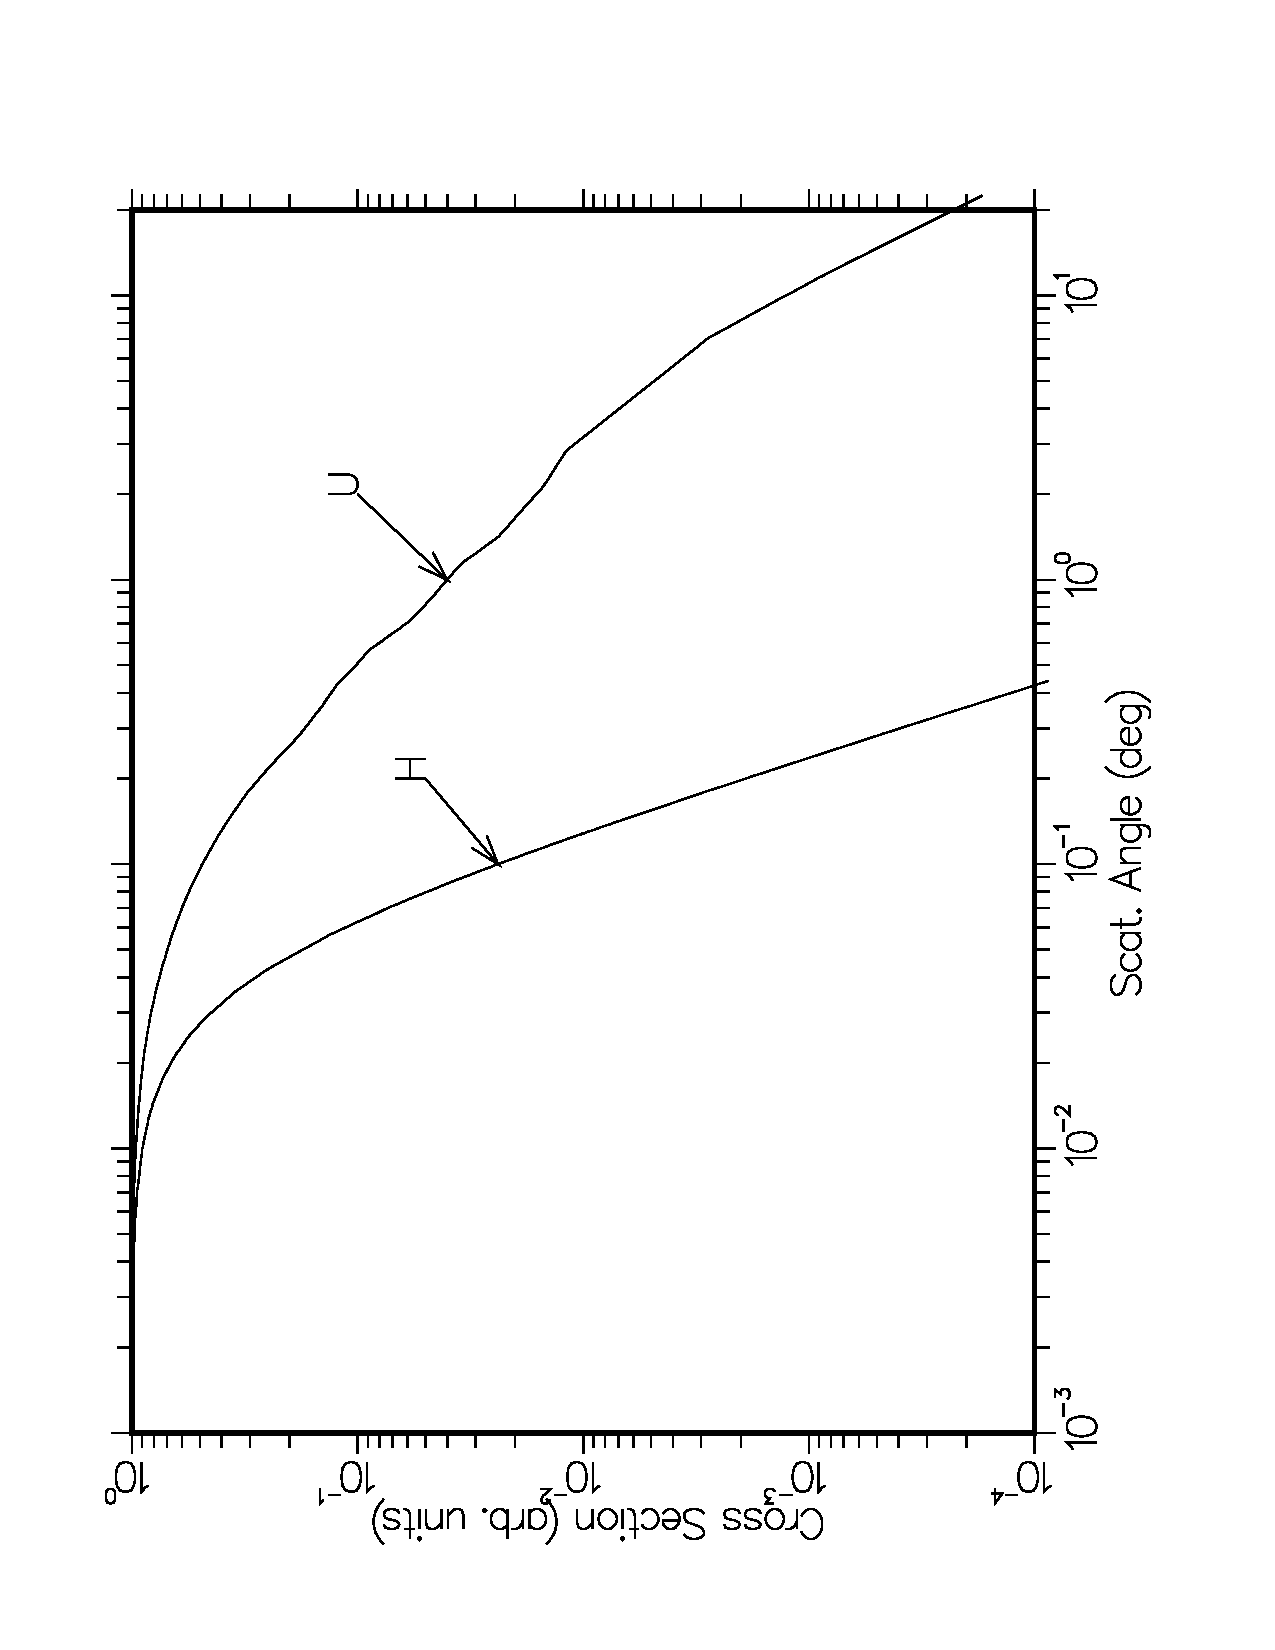
\includegraphics[keepaspectratio, height=3.5in, angle=270]{figs/gaminr1ack}
\caption[Photon coherent scattering angular distributions]{Angular distribution
 for coherent scattering from hydrogen and uranium at high photon energy.}
\label{fig1}
\end{figure}

For coherent scattering, the integral of Eq.~\ref{eq10} is broken up
into panels  by the tabulation values of $x$.  Each panel is integrated
in the $x$ domain using Lobatto quadrature of order 6 for $\ell=3$
or less and order 10 for larger Legendre orders.  Eq.~\ref{eq2}
is used to compute the $\mu$ value for each $x$ and to obtain the
Jacobian required.

Since $\mu$ is quadratic in $x$, the polynomial order of the integrand
in the numerator of Eq.~\ref{eq10} is $2\ell+2$ plus twice the polynomial
order of $F$ in the panel.  For $\ell=3$, the theory of Gaussian quadrature
implies that the integral will be exact if $F$ can be represented as a
quadratic function over the panel.

The incoherent integral of Eq.~\ref{eq11} is also broken up into panels,
but here the panels are defined by the union of the tabulation values
of $x$ and the momenta corresponding to the secondary-energy group
bounds.  The relationship between $x$, $\mu$, and secondary energy is given
in Eqs.~\ref{eq5} and \ref{eq6}.  This time, the integral is
performed {\it vs.} $E'$ using Lobatto quadrature\index{Lobatto quadrature}
of order 6 for $\ell$ less than or equal to 5 and order 10 for
larger $\ell$ values.

All form factors and structure factors are interpolated using
ENDF/B log-log interpolation as specified by the format.  However, the
cross sections in the file were evaluated using a special
log-log-quadratic scheme.  Ignoring this complication may lead to a 5\%
error in the incoherent cross section at 0.1 keV with a negligible
error at the higher energies that are of most practical
concern\cite{Hubbell}.

\subsection{Coding Details}
\label{ssGAMINR_details}

The main entry point is subroutine \cword{gaminr} exported by
module \cword{gaminm}\index{modules!gaminm@{\ty gaminm}}.
The code begins by reading the user's input.  It then locates the
position for the new material on the old GENDF\index{GENDF}
tape (if any) and copies the earlier results to the new output
tape.  The desired material is also located on the input
PENDF\index{PENDF} tape prepared previously using
\hyperlink{sRECONRhy}{RECONR}\index{RECONR}.
A new material header is then written onto the output tape leaving
the code ready to begin the loop over reaction types.

For each of the preset reaction types, GAMINR uses the panel logic
of \hyperlink{sGROUPRhy}{GROUPR}\index{GROUPR} to
average the cross sections (see the ``panel" discussion
in Section~\ref{ssGROUPR_GrpInt}).  If this is the first material
in a series of elements, the incoherent matrix is saved to a scratch area.
For subsequent materials, the higher energy matrix elements are obtained
by scaling these saved values by the appropriate $Z$ ratio.  The
resulting cross sections and group-to-group matrix elements are then
printed out and written to the output tape.  The heat production
contribution from each reaction is summed into a storage area.  After
all reactions have been processed for this material, a special pass
through the output logic is used to create a heating section using
MT=525 for ENDF/B-VI and later files or MT=525 for earlier
ENDF/B files.  Finally, the rest of the
old output tape is copied to the new output tape.  A description of the
format of the multigroup output tape will be found in the
\hyperlink{sGROUPRhy}{GROUPR} chapter
(see Section~\ref{ssGROUPR_GENDF}).

As with \cword{panel} in
\hyperlink{sGROUPRhy}{GROUPR}, \cword{gpanel}\index{gpanel@{\ty gpanel}}
integrates the triple product ${\cal F}{*}\sigma{*}\phi$.  The feed into
secondary group $g'$ for Legendre order $\ell$ from initial energy $E$
is computed in \cword{gtff}\index{gtff@{\ty gtff}} as described in
Section~\ref{ssGAMINR_FormFact} above.  Cross sections are read from
the PENDF tape (see
\cword{gtsig}\index{gtsig@{\ty gtsig}}).  Flux can be read in,
constant, or $1/E$ with high and low energy roll-offs (see
\cword{gnwtf}\index{gnwtf@{\ty gnwtf}} and
\cword{gtflx}\index{gtflx@{\ty gtflx}}).

\subsection{User Input}
\label{ssGAMINR_UserInp}

The following description of the user input is reproduced from
the comment cards at the beginning of the GAMINR module.
\index{GAMINR!GAMINR input}
\index{input!GAMINR}

\small
\begin{ccode}

   !---input specifications (free format)---------------------------
   !
   ! card1
   !    nendf   unit for endf tape
   !    npend   unit for pendf tape
   !    ngam1   unit for input ngam tape (default=0)
   !    ngam2   unit for output ngam tape (default=0)
   ! card2
   !    matb    material to be processed
   !            input materials in ascending order
   !    igg     gamma group structure option
   !    iwt     weight function option
   !    lord    legendre order
   !    iprint  print option (0/1=minimum/maximum) (default=1)
   ! card3
   !    title   run label up to 80 characters (delimited by ',
   !            ended with /)
   ! card4      (igg=1 only)
   !    ngg     number of groups
   !    egg     ngg+1 group bounds (ev)
   ! card5      (iwt=1 only)
   !    wght    weight function as tab1 record
   ! card6
   !    mfd     file to be processed
   !    mtd     section to be processed
   !    mtname  description of section to be processed
   !            repeat for all reactions desired
   !            mfd=0/ terminates this material
   !            mfd=-1/ is a flag to process all sections present
   !            for this material  (termination is automatic)
   ! card7
   !    matd    next mat number to be processed
   !            terminate gaminr run with matd=0.
   !
   !---options for input variables----------------------------------
   !
   !        igg     meaning
   !        ---     -------
   !         0      none
   !         1      arbitrary structure (read in)
   !         2      csewg 94-group structure
   !         3      lanl 12-group structure
   !         4      steiner 21-group gamma-ray structure
   !         5      straker 22-group structure
   !         6      lanl 48-group structure
   !         7      lanl 24-group structure
   !         8      vitamin-c 36-group structure
   !         9      vitamin-e 38-group structure
   !         10      vitamin-j 42-group structure
   !
   !        iwt     meaning
   !        ---     -------
   !         1      read in
   !         2      constant
   !         3      1/e + rolloffs
   !
   !------------------------------------------------------------------

\end{ccode}
\normalsize

Note that both an ENDF/B tape and a PENDF tape from
\hyperlink{sRECONRhy}{RECONR} are required.
Older, pre-ENDF/B-VI, photon interaction tapes are available from the Radiation
Shielding Information Computational Center (RSICC) at ORNL
as DLC7E (for ENDF/B-IV) or DLC-99/HUGO (for ENDF/B-V).
A photoatomic library in ENDF-6 format based on DLC-99 is available
from the National Nuclear Data Center (NNDC) at the Brookhaven National
Laboratory.  The latest photoatomic library is also available
from the NNDC.  Material numbers (\cword{matb}) are simply the element
$Z$ number for versions IV and V;  they are equal to $100{*}Z$ for
ENDF-6 formatted files.  The values of \cword{matd} on card 7 should
be given in increasing order for maximum economy.  The normal mode
of operation uses \cword{mfd}$=-1$.  This automatically processes
MT=501, 502, 504, 516, 522, and 525.  For pre-ENDF-6 formatted files,
the photoelectric cross section is changed from 522 to 602, and the
heating cross section is changed from 525 to 621.

The following sample run prepares a GENDF tape for two elements.
The numbers on the left are for reference; they are not part of the input.

\small
\begin{ccode}

  1.   reconr
  2.   20 21/
  3.   'pendf tape for 2 elements from ENDF/B-VII'/
  4.   100 1 0/
  5.   .001 0./
  6.   '1-hydrogen'/
  7.   9200 1 0/
  8.   .001 0./
  9.   '92-uranium'/
 10.   0/
 11.   gaminr
 12.   20 21 0 22/
 13.   100 7 3 4 0/
 14.   '24-group photon interaction library'/
 15.   -1/
 16.   9200/
 17.   -1/
 18.   0/
 19.   stop

\end{ccode}
\normalsize

On line 2, an ENDF/B tape containing File 23 has been
mounted on logical unit 20.  The title on line 3 will appear on the PENDF
tape.  Material 100 is hydrogen (lines 4-6) and material 9200 is uranium
(lines 7-9).  The element names on lines 8 and 11 will appear on the
PENDF tape in MF=1,MT=451.  Linearization is accurate to better
than 0.1\%.  A more complete description of
\hyperlink{sRECONRhy}{RECONR's} input may be found in
Section~\ref{ssRECONR_inp}.

GAMINR uses the same ENDF tape as \hyperlink{sRECONRhy}{RECONR}
(actually only MF=27 is read
by GAMINR), but GAMINR also reads the
\hyperlink{sRECONRhy}{RECONR} output tape on unit 21.
The GAMINR GENDF tape will be on unit 22.  Card 13 specifies hydrogen
as the first material, 24 groups, $1/E$ weight with roll-offs,
Legendre components through P$_3$, and the full printed output.  Cards 16
and 17 select the default list of reaction types.  Card 16 specifies
uranium as the second material to be processed, and line 18 terminates
the element loop and the GAMINR run.

Figs.~\ref{fig2} and \ref{fig3} illustrate plots of the results of this
sample run.  These graphs were made using the
\hyperlink{sDTFRhy}{DTFR} and \hyperlink{sVIEWRhy}{VIEWR} modules.

\begin{figure}[p]\centering
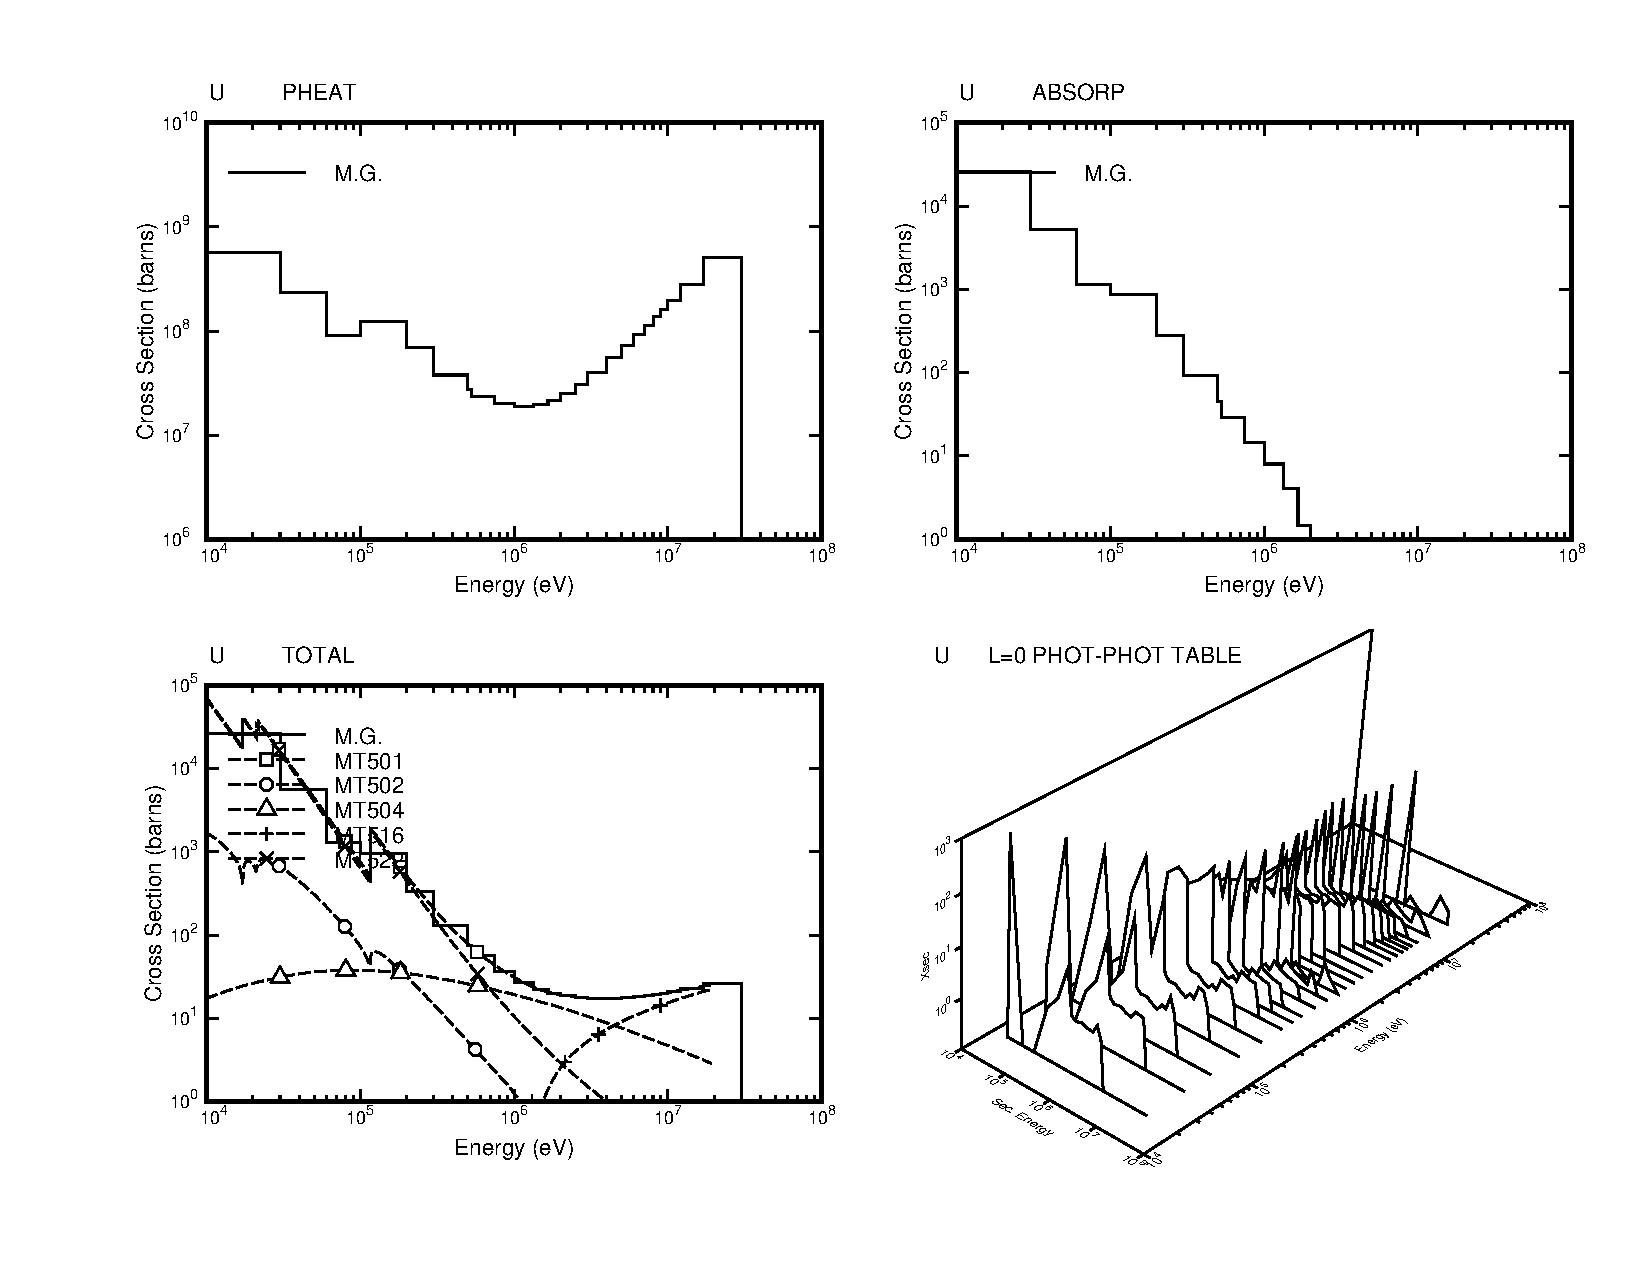
\includegraphics[keepaspectratio, width=4.5in, angle=0]{figs/gaminr2ack}
\caption[Photon interaction cross sections for uranium]{Plots of the photon
 interaction cross sections and the photon scattering distribution for uranium
 showing both 24-group and continuous cross sections.  Note the prominent
 photoelectric absorption edge near 100 keV.}
\label{fig2}
\end{figure}

\begin{figure}[p]\centering
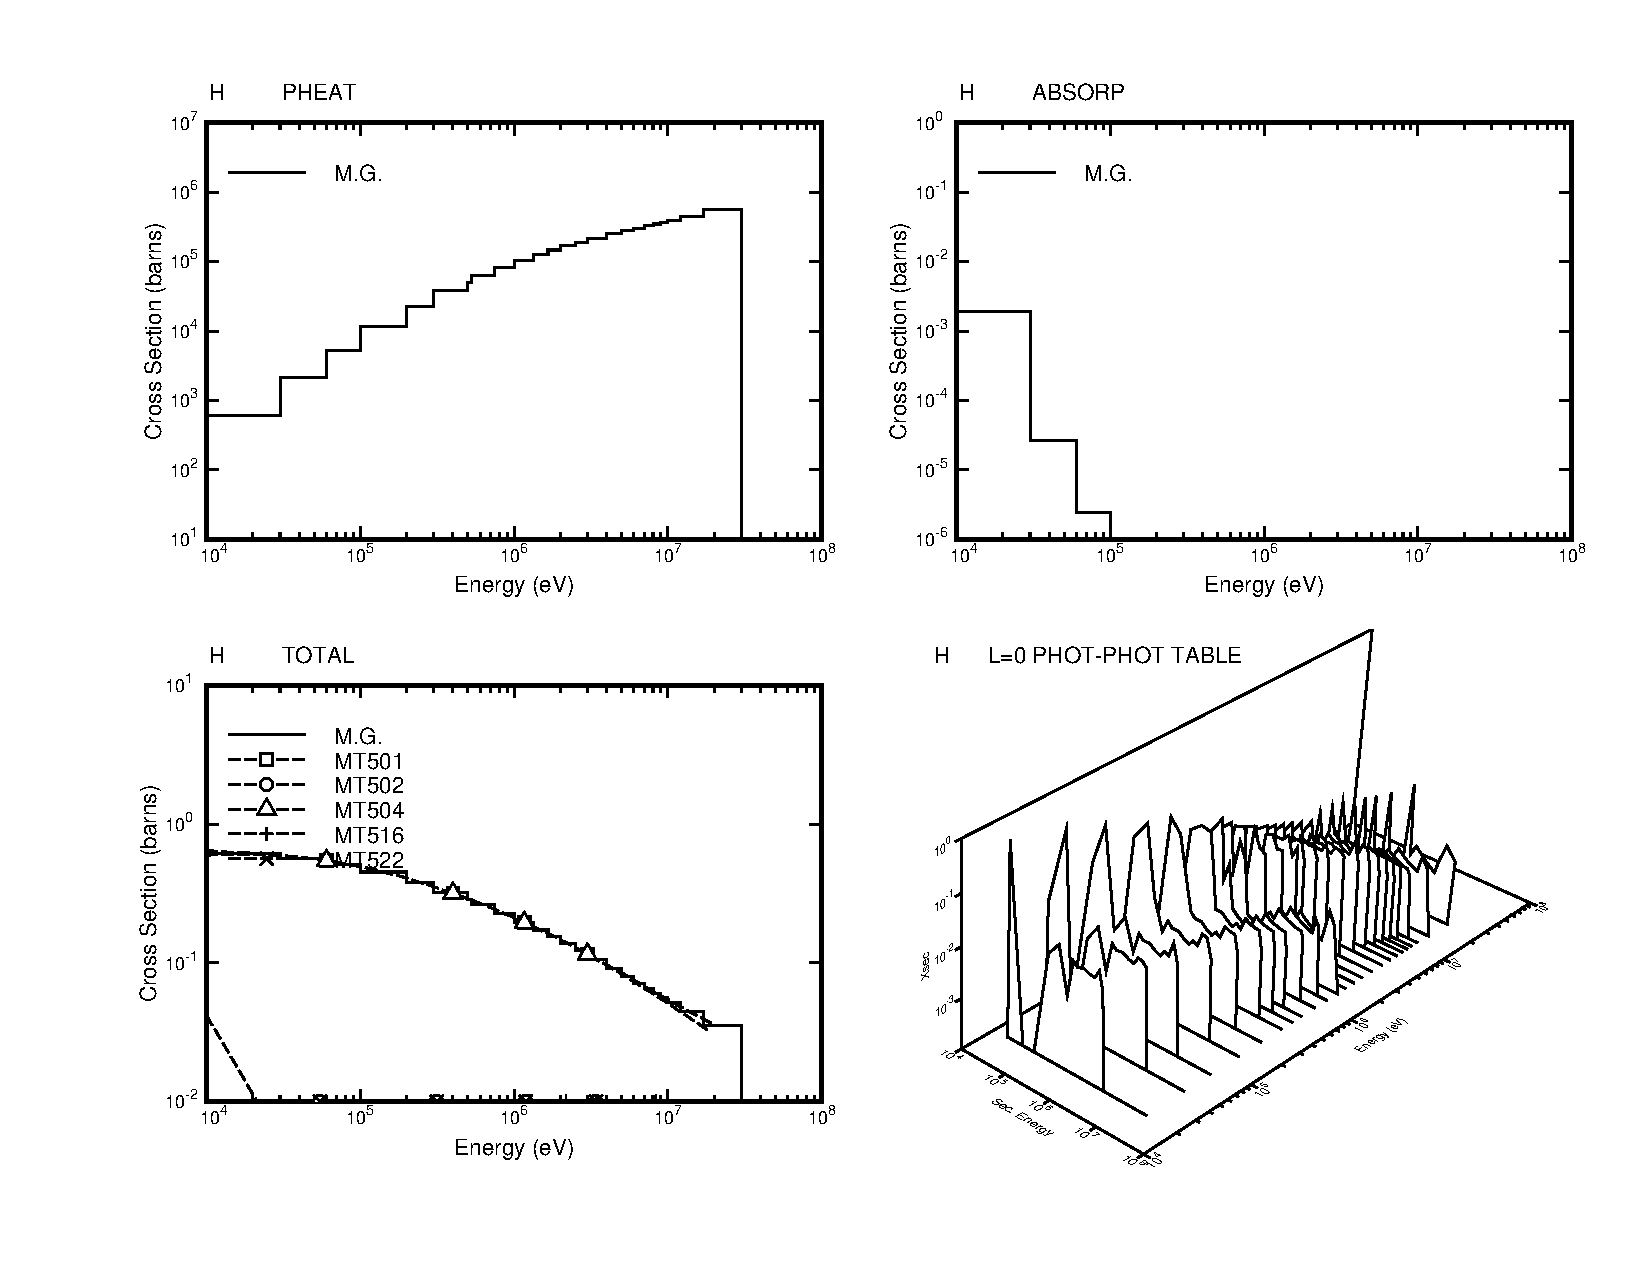
\includegraphics[keepaspectratio, width=4.5in, angle=0]{figs/gaminr3ack}
\caption[Photon interaction cross sections for hydrogen]{Plots of the photon
 interaction cross sections and the photon scattering distribution for hydrogen
 showing both 24-group and continuous cross sections.  The cross sections
 are simpler for this case.}
\label{fig3}
\end{figure}

Starting with ENDF/B-VI, the photon interaction (or photoatomic)
files contain detailed photoelectric cross sections, not just
the MT=522 total photoelectric cross section.  These photoelectric
cross sections have MT numbers starting with 534.  As an example,
Fig.~\ref{shells} shows the first 9 partial cross sections for
uranium --- the K, L, and M subshells --- taken from ENDF/B-VII.
GAMINR input is somewhat more complicated when these reactions
are included because they are different for every element.

\begin{figure}[thb]\centering
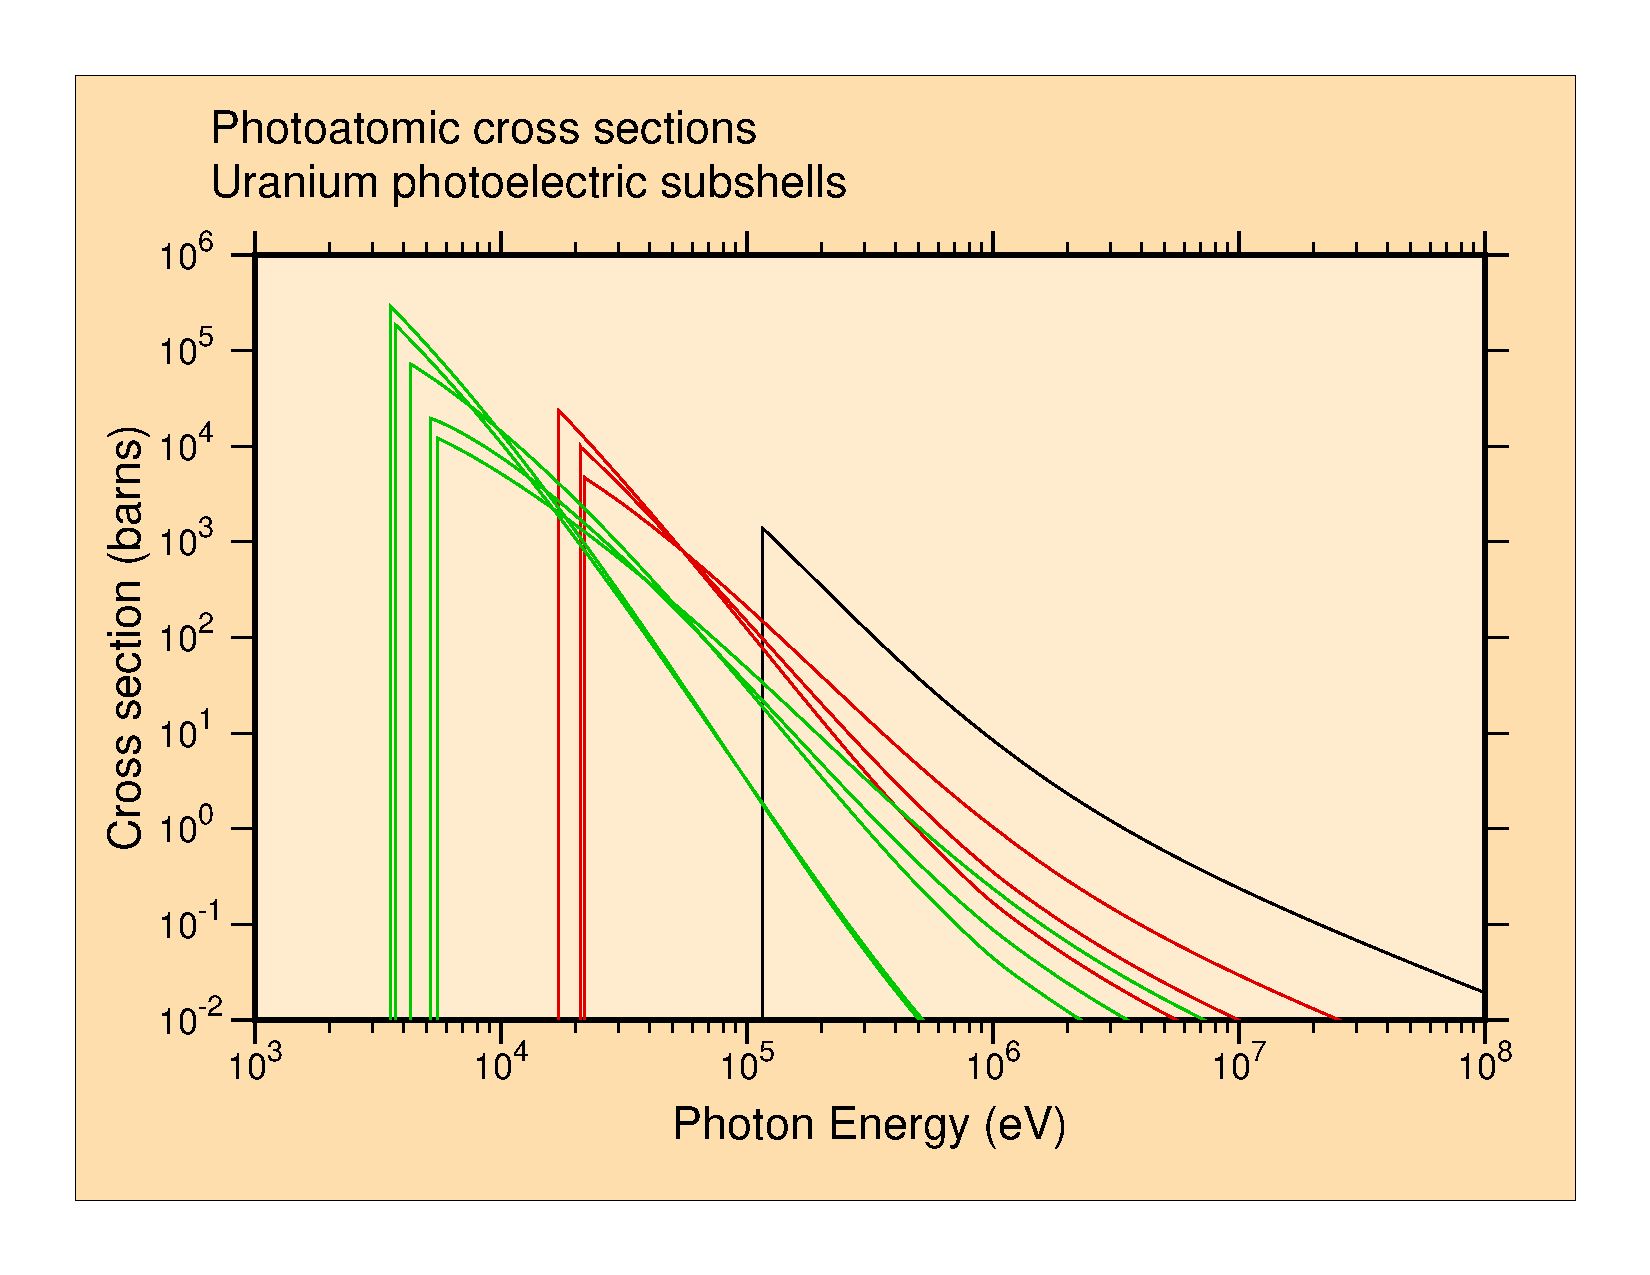
\includegraphics[keepaspectratio, width=4.0in,angle=0]{figs/gaminr4ack}
\caption[ENDF/B-VII.0 Uranium photoelectric subshell cross sections]{The
 first nine photoelectric subshell cross sections for uranium from
 ENDF/B-VII.0.  Black is the S subshell (1s$^{1/2}$), red is the L1, L2,
 and L3 subshells (2s$^{1/2}$, 2p$^{1/2}$, 2p$^{3/2}$), and green is the
 M1 through M5 subshells (3s$^{1/2}$, 3p$^{1/2}$, 3p$^{3/2}$, 3d$^{3/2}$,
 3d$^{5/2}$).}
\label{shells}
\end{figure}

\subsection{I/O Units}
\label{ssGAMINR_IO}

There are no scratch files used in GAMINR.  The only restriction
on the files assigned on line 1 of the user input is that \cword{ngam1} and
\cword{ngam2} must be in the same mode (that is, both binary or both
formatted).

\subsection{Error Messages}

\begin{description}
\begin{singlespace}

\item[\cword{error in genggp***illegal group structure}] ~\par
  Values of \cword{IGG} must lie between 1 and 10.

\item[\cword{error in genggp***too many groups.}] ~\par
  Increase the size of the global array \cword{egg} by changing the
  parameter \cword{ngmax}=400 located at the start of the module.

\item[\cword{error in gnwtf***illegal iwt}] ~\par
  Values of \cword{iwt} must lie between 1 and 3.

\item[\cword{error in gpanel***elo gt ehi.}] ~\par
  There is something wrong with the energy grids during integration
  over incident energy. This usually means there is a problem with
  the choice of \cword{rndoff} and/or \cword{delta}.  Be sure that
  \cword{rndoff}$<$1, \cword{delta}$>$1, and \cword{rndoff*delta}$<$1
  as represented on your machine.

\item[\cword{ERROR IN GTFF***ILLEGAL FILE TYPE.}] ~\par
  Only files 23 and 26 can be requested.

\item[\cword{error in gtff***illegal reaction for cross section=---}] ~\par
  Only reactions 501, 502, 504, 516, 602, and 621 (heat) can be requested
  for ENDF/B-IV or -V, or only 501, 502, 504, 516, 522, and 525 for
  ENDF/B-VI or VII.

\item[\cword{error in gtff***insufficient storage for form factor.}] ~\par
  This refers to the allocatable array \cword{pff} with size
  \cword{nwpff}=5000 defined in the main \cword{gaminr} routine.

\end{singlespace}
\end{description}

\cleardoublepage


\section{ERRORR}
\label{sERRORR}
\index{ERRORR|textbf}

\hypertarget{sERRORRhy}{The}
ERRORR module is used to produce cross section and distribution
covariances from error files in ENDF format.

This chapter describes the ERRORR module in NJOY2016.0.

\subsection{Introduction}
\label{ssERRORR_Intro}

After evaluators have completed their review of the available
measurements of various nuclear data (having true values $\sigma_{1},
\sigma_{2}, \sigma_{3},\cdots$) and the theoretical analysis, they will
have formed at least a subjective opinion of the joint probability
distribution of the data examined; that is, the probability
\[ P(\sigma_{1},\sigma_{2},\cdots) \, d\sigma_{1}\, d\sigma_{2}\cdots\]
that the true value of $\sigma_1$ lies in the range $(\sigma_1,
\sigma_1 {+} d\sigma_1)$, and that $\sigma_2$ lies in the range
$(\sigma_2, \sigma_2 {+} d\sigma_2)$, etc.  In the early versions
of the ENDF format, only the first moments (expectation values) of this
probability distribution could be included in the numerical data
files.  However, beginning with ENDF/B-IV and expanding significantly
in ENDF/B-V and later, the second moments of the data
probability distributions have been included in many of the files.
As discussed in Section~\ref{ssERRORR_Defs}, these second moments
(or ``data covariances'')
contain information on the uncertainty of individual data, as well as
correlations that may exist.  Fig.~\ref{b10cov} shows an example of
this for $^{10}$B from ENDF/B-VII.0.  The top plot shows the first
moment (the percent standard deviation) of the uncertainty in the
(n,$\alpha$) cross section.  The right-hand plot shows the cross
section.  The center plot shows the correlations between the
(n,$\alpha$) cross section at one energy to itself at other energies.
\index{covariances}

\begin{figure}[thb]\centering
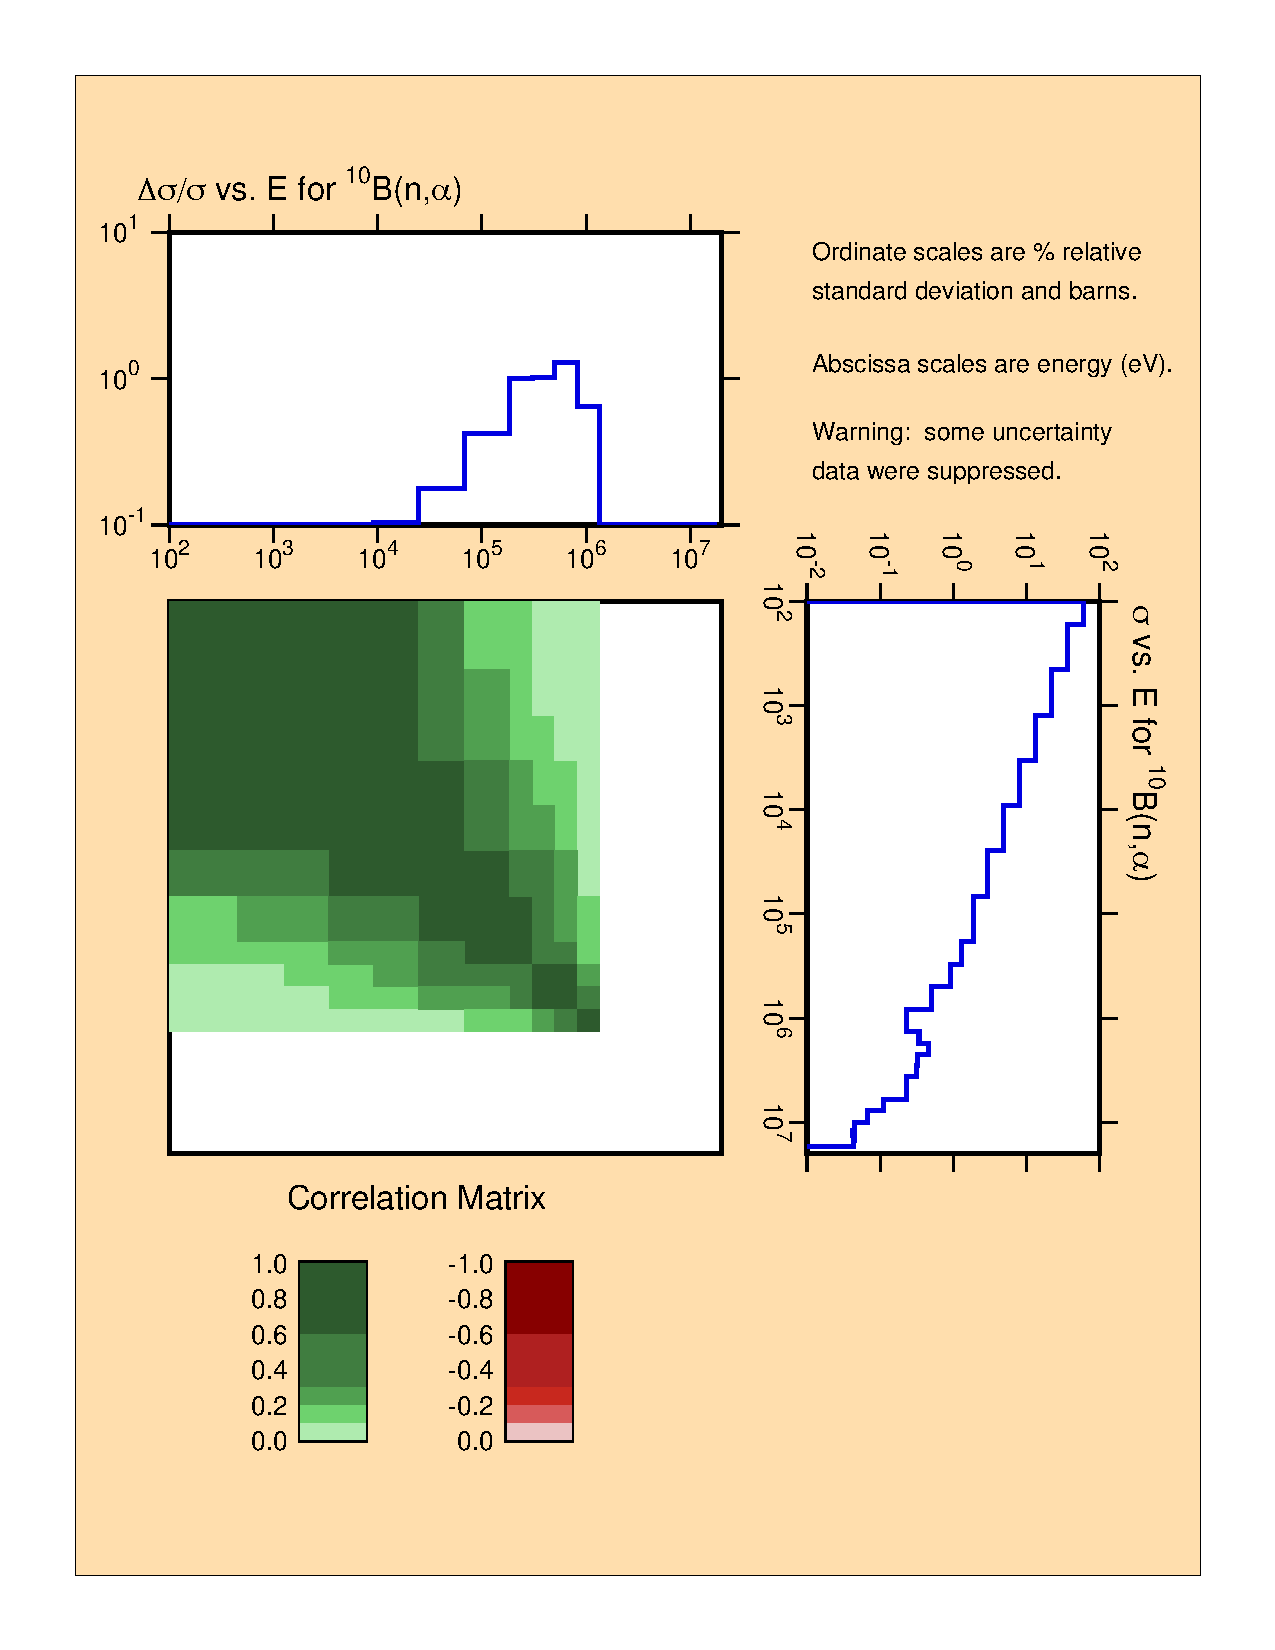
\includegraphics[keepaspectratio, width=5.0in,angle=0]{figs/b10covack}
\caption[ENDF/B-VII.0 $^{10}$B(n,$\alpha$) covariance data]{Covariance
 plot for $^{10}$B(n,$\alpha$) from ENDF/B-VII.0.  This reaction is used as
 a standard in the ENDF system.}
\label{b10cov}
\end{figure}

Data covariances have many applications.  For example, they can be
combined with sensitivity coefficients to obtain the uncertainty, due
to the data, in calculated quantities of applied interest\cite{Gerstl}.
This information can be used in turn to judge the adequacy of the data
for that application.
\index{sensitivity analysis}

The availability of data covariances also makes it possible to use the
generalized method of least squares to improve the data evaluation
after new integral or differential measurements have been
performed\cite{Reupke}.  The least-squares method requires only data
covariances (not the full probability distribution), and the improved,
or adjusted, data are guaranteed\cite{Hamilton} to have the smallest
possible uncertainties, regardless of the actual shape of the underlying
probability distribution function, $P(\sigma_1, \sigma_2,\cdots)$.
\index{data adjustment}
Thus, the ENDF-formatted covariance files contain, in about as compact
a form as possible, a statement about the quality of the data, as well
as sufficient information (in principle) to carry out future
improvements on an objective basis.

In many of these applications, it is necessary to begin by converting
energy-dependent covariance information in ENDF format\cite{ENDF102}
into multigroup form.  This task can be performed conveniently in the
NJOY environment, using the ERRORR module.  In particular,
ERRORR calculates the uncertainty in infinitely dilute multigroup cross
sections (or multigroup $\bar{\nu}$ values), as well as the associated
correlation coefficients.  These data are obtained by combining
absolute or relative covariances from ENDF Files 31, 32, 33, 34, 35 and 40
with multigroup $\bar{\nu}$ data, cross section data, angular disbribution
data, fission spectra data or radionuclide production data.  These
multigroup data are obtained from \hyperlink{sGROUPRhy}{GROUPR}
processing, or in some instances are calculated
within ERRORR.  ERRORR is coded to treat all approved ENDF-4, -5, and -6
covariance formats for these files.  ERRORR can also treat
resolved-resonance covariances given in File 32 using the old
Breit-Wigner resolved-resonance parameter uncertainties (\cword{LRF}=1
and \cword{2}) in Version-5 format, the ``Version-5 compatible''
option of Version 6 (\cword{LCOMP}=0) using the new formats
that include resonance-resonance covariances, and the newest
format based on Reich-Moore-Limited parameters that include
resonance-resonance correlations between different reactions.

The methodology of ERRORR assumes that the weighting flux
\index{weighting flux} used to convert energy-dependent cross sections
into multigroup averages is free of uncertainty.  In cases in which
the cross-section information is obtained from an existing multigroup
library, it is usually necessary to make assumptions about the shape
of the cross section and the weight function within certain input
energy groups.

\subsection{Definitions of Covariance-Related Quantities}
\label{ssERRORR_Defs}

For convenient reference in discussing the methodology and input
requirements of the ERRORR module, we next review the basic definitions
of covariance-related quantities.  Let $x_{0}$ and $y_{0}$ be the
evaluated values of $x$ and $y$, respectively:

\begin{equation}
   x_{0} \equiv {\rm E}[x] \; ,
\end{equation}

\noindent
and

\begin{equation}
   y_0 \equiv {\rm E}[y] \; .
\end{equation}

\noindent
Here E is the expectation operator, which performs an average over the
joint probability distribution of $x$ and $y$.  The second moment of
this distribution is called the covariance of $x $ with $y$:

\begin{equation}
{\rm cov} (x,y) \equiv {\rm E}[(x\;-\;x_0)\;(y\;-\;y_0)]\;.
\label{cov}
\end{equation}

\noindent
Covariance is a measure of the degree to which $x$ and $y$ are both
affected by the same sources of error.  The covariance of $x$ with
itself is called the variance of $x$:

\begin{equation}
{\rm var}(x) \equiv {\rm cov}(x,x) = {\rm E}[(x\;-\;x_0)^2]\;.
\end{equation}

\noindent
The more familiar standard deviation $\Delta x$ (also called the
``uncertainty'') is simply

\begin{equation}
\Delta x \equiv [{\rm var} (x)]^{1/2} = [{\rm cov}(x,x)]^{1/2} \; .
\label{deltax}
\end{equation}

\noindent
The correlation between $x$ and $y$ (also called the correlation
coefficient) is defined as

\begin{equation}
{\rm corr}(x,y) \equiv \frac{{\rm cov}(x,y)}{\Delta x\;\Delta y} \;.
\label{corr}
\end{equation}

\noindent
The absolute value of a correlation coefficient is guaranteed to be
less than or equal to unity.  Another useful quantity is the relative
covariance of $x$ with $y$,

\begin{equation}
{\rm rcov}(x,y) \equiv \frac {{\rm cov}(x,y)}{x_0 \; y_0} \;.
\label{rcov}
\end{equation}

\noindent
Unlike ${\rm cov}(x,y)$, the relative
{\rm cov}ariance ${\rm rcov}(x,y)$ is a dimensionless quantity.
Closely related to the relative covariance is the relative standard
deviation,

\begin{equation}
\frac {\Delta x}{x_0} \;=\; \frac {[{\rm cov}(x,x)]^{1/2}}{x_0} \;,
\end{equation}

\noindent
which, from Eq.~\ref{rcov}, can be written as

\begin{equation}
\frac {\Delta x}{x_0}\; =\; [{\rm rcov}(x,x)]^{1/2} \; .
\label{deltax0}
\end{equation}

\noindent
Combining Eqs.~\ref{corr} and \ref{rcov}, we have another useful result,

\begin{equation}
{\rm corr}(x,y) = \frac{{\rm rcov}(x,y)}{(\Delta x/x_0) (\Delta y/y_0)}\;.
\label{corr2}
\end{equation}

While it is customary to speak of uncertainties\index{uncertainties}
and correlations\index{correlations} as separate entities, these
are actually just two different aspects of the covariance.  If one
has a set of absolute covariances for various reactions, including
the self-covariance, then Eqs.~\ref{deltax} and \ref{corr} can be used
to calculate $\Delta x$ and corr$(x,y)$.  Similarly, if one has a set
of relative covariances, one can use Eqs.~\ref{deltax0} and
\ref{corr2} to calculate $\Delta x/x_0$ and corr$(x,y)$.

Consider now a set of nuclear data $\sigma_i$ with uncertainties
characterized by the covariances {\rm cov}$(\sigma_i,\sigma_j)$.  Let
$A$ and $B$ be two linear functions of the $\sigma_i$,

\begin{equation}
A =\sum_{i} \; a_i \; \sigma_i
\end{equation}

\noindent
and

\begin{equation}
B =\sum_{j} \; b_j \; \sigma_j \; ,
\end{equation}

\noindent
where the $a_i$ and $b_j$ are sets of known constants.  The above
definitions can be used to calculate the covariances of the functions
$A$ and $B$ induced by the covariances of the data.
From Eq.~\ref{cov},

\begin{eqnarray} {\rm cov}(A,B) & = & {\rm E} \left\{ {\vphantom{\sum_j}}\left
({\vphantom{\sum_j}}\sum_{i} \; a_i \; \sigma_i \; - \;\sum_{i}\; a_i {\rm E}
(\sigma_i)\right)\;{\vphantom{\sum_j}}\left(\sum_{j} \;b_j \;\sigma_j - \sum_{j}
(\sigma_j )\right )\right \} \nonumber \\
 & = & \sum_{i,\; j} \; a_i \; b_j \; {\rm E} \left \{ {\vphantom{\sum}}\left
({\vphantom{\sum}}\sigma_i
 {-}  {\rm E} (\sigma_i)  \right ) \;
 \left ({\vphantom{\sum}} \sigma_j{-}{\rm E} (\sigma_j) \right)  \right \}  \;,
\end{eqnarray}

\noindent
so that

\begin{equation}
{\rm cov}(A,B) = \sum_{i,\,j} \; a_i \; b_j \; {\rm cov}(\sigma_i , \sigma_j ) \
\label{e11}
\end{equation}

\noindent
This result, called the ``propagation of errors'' formula, is
fundamental to the subject of multigroup processing of ENDF covariance
data and will be referenced frequently in later sections of this
chapter.

\subsection{Structure of ENDF Files 31, 33, and 40: Energy-Dependent Data}
\label{ssERRORR_Str}

Data in ENDF format are stored in various numbered ``files,'' where the
file number depends on the type of information contained.  For example,
the covariances of $\bar{\nu}(E)$ (the average number of neutrons per
fission, which is a function of the incident neutron energy) are stored
in File 31, where the possible ``reaction'' types are prompt
$\bar{\nu}$, delayed $\bar{\nu}$, and total $\bar{\nu}$.  File 33
contains the covariances of energy-dependent cross sections.  In
general, for data given in File N, covariance data are given in
File (N+30).  The structures of Files 31, 33, and 40 are identical
and will be described first.

Files 31, 33, and 40 describe the covariances of energy-dependent data.  To
expand on this point, we recall that the full energy dependence of a
cross section $\sigma (E)$, for example, is described in the ENDF File
3 by specifying the cross-section values at a relatively small number
of energy points and then providing a set of interpolation laws to be
used in reconstructing the actual cross section at any intermediate
energy.  Somewhat the same philosophy is used to describe the
two-dimensional energy dependence of data covariances in Files 31, 33, and
40.  That is, one specifies a set of numerical data and a set of
formulae, which together can be used to compute ${\rm cov}(x,y)$ for
any desired pair of energies, $E_x$ and $E_y$.  Although
the interpolation laws are presently restricted to the simple forms
described below, it is not true (as sometimes stated) that ENDF
contains multigroup covariances.  The expression ``multigroup
covariance'' refers to the covariance of one multigroup-averaged
quantity with another averaged quantity, whereas ENDF contains the
covariances between point-energy data.  It is precisely the task of
ERRORR to compute multigroup covariances, starting from point
covariances.

Files 31, 33, and 40 of an evaluation for material \cword{MAT} are divided
into ``sections,'' indexed by the reaction type \cword{MT}.  A section
\cword{(MAT,MT)} is further subdivided into ``subsections.''  As
described in the ENDF formats manual, a subsection is the repository
for all explicit statements of the two-dimensional energy dependence
of the covariances of reaction \cword{(MAT,MT)} with another reaction
\cword{(MAT1,MT1)}.  Because covariances are symmetric, a subsection
with \cword{MAT1}=\cword{MAT} and \cword{MT1}$<$\cword{MT} would be
redundant with a subsection in an earlier section, and such data are,
by convention, omitted from the ENDF files.

Subsections are further divided into ``sub-subsections.''  Two different
types of sub-subsections are used in the ENDF-5 and ENDF-6 formats.  ERRORR
also treats data covariances in the earlier
ENDF-4 format, but this is of little practical interest since only three
covariance evaluations were released in the Version-4 format.  ``NI-type''
sub-subsections are used to express covariances explicitly, while
``NC-type'' sub-subsections are used to indicate the existence of
connections between various data that result in ``implicit'' covariance
contributions for various reaction pairs.  We shall return to this
point when discussing NC-Type Sub-Subsections.

\paragraph{NI-Type Sub-Subsections.} Multiple NI-type sub-subsections
are used to describe multiple, statistically independent sources of
uncertainty for a given reaction pair.  If $ {\rm cov}(x,y)_n$ is the
covariance computed from the data in one sub-subsection, then, because
the uncertainties in different sub-subsections are uncorrelated,
$$
{\rm cov}(x,y) \;= \; \sum^{{\rm NI}}_{n=1} \; {\rm cov}(x,y)_n \; ,
$$
\vspace{2 pt}
where NI is the number of NI-type sub-subsections in the current
subsection.\ The numerical content of one NI-type sub-subsection
consists of either one or two energy grids, a collection of constants,
and a parameter \cword{LB}.  The parameter \cword{LB} governs how the
energies and constants are to be used in constructing the covariance in
various rectangular regions of $E_x {-}E_y$ space.  For \cword{LB}=0, 1,
2 and 8, a single table containing pairs $(E_i,F_i)$ is
given.  For \cword{LB}=3 and \cword{LB}=4, two such tables are given.  For
\cword{LB}=5,  a single set of energies $E_i$ is given, along with an
associated square matrix of constants $G_{ij}$.  Finally, for
\cword{LB}=6, two energy grids are given, along with an associated
rectangular matrix of constants $G'_{ij}$.

The first of these tables $(E_i,F_i)$ defines a function $f(E)$
that is constant except for
discrete steps at energies $E_i$,

\begin{equation}
f(E) = F_i ,\;{\rm if}\; E_i{\leq} E{<}E_{i+1} \;.
\label{e12}
\end{equation}
\vspace{0.5 pt}

\noindent
Similarly, if there is a second table,

\begin{equation}
f'(E) = F'_j , \; {\rm if}\; E'_j{\leq}E{<}E'_{j+1} \;.
\end{equation}
\vspace{0.5 pt}

\noindent
The \cword{LB}=5 matrix data $G_{ij}$ also define a function,

\begin{equation}
g(E_x,E_y) = G_{ij},\, {\rm{if}}\; E_i {\leq} E_x{<}E_{i+1} \;{\rm {and}}\; E_j
\; , \end{equation}

\noindent
and similarly for \cword{LB}=6

\begin{equation}
g'(E_x,E_y) = G'_{ij}, \, {\rm {if}}\;  E_i  {\leq} E_x {<} E_{i+1}\;{\rm {and}}
{\leq} E_y{<}E'_{j+1} \;.
\end{equation}
\vspace{1 pt}

\noindent
These functions are simply histograms in either one or two dimensions.
Using the functions $f$, $f'$, $g$, and $g'$ thus defined, we can list
the formulae in Eq.~\ref{lbopts}, which are used to specify energy-dependent
covariances for the different allowed values of \cword{LB}.  Thus, if
$x$ is the value of the cross section or of the $\bar{\nu}$ value for the
reaction \cword{(MAT,MT)} that determines the ENDF/B
\underline{section}, and if $y$ is the value for the reaction
\cword{(MAT1,MT1)} that determines the \underline{subsection}, then for

\begin{equation}
\begin{array} {rrrll}
{\rm {LB}} & = & 0, &  {\rm {{\rm cov}}} (x,y)_n   & = \; f (E_x) \,
  \delta (E_x,E_y)   \\
{\rm {LB}} & = & 1, &  {\rm {r{\rm cov}}} (x,y)_n  & =  \; f (E_x) \,
  \delta (E_x,E_y)  \\
{\rm {LB}} & = & 2, &  {\rm {r{\rm cov}}} (x,y)_n  & =  \; f (E_x)\,f(E_y)  \\
{\rm {LB}} & = & 3, &  {\rm {r{\rm cov}}} (x,y)_n  & =  \;f (E_x)\,f'(E_y) \\
{\rm {LB}} & = & 4, &  {\rm {r{\rm cov}}} (x,y)_n  & = \; f (E_x) \,
  \delta (E_x,E_y)\;f'(E_x)\,f'(E_y)
\\ {\rm {LB}} & = & 5, &  {\rm {r{\rm cov}}} (x,y)_n  & =  \;g (E_x,E_y)  \\
{\rm {LB}} & = & 6, &  {\rm {r{\rm cov}}} (x,y)_n  & = \; g'(E_x,E_y)\,\,.
\end{array}
\label{lbopts}
\end{equation}

\noindent
The symbol $\delta (E_x,E_y)$ has the following meaning: $\delta
(E_x,E_y){ =} 1$ if $E_x$ and $E_y$ fall in the same energy interval of
the first table $(E_i$, $F_i$), and $\delta(E_x,E_y){ =} 0$ otherwise.

The final covariance law, \cword{LB}=8, is an exceptional case that
cannot be expressed in terms of point covariances.  \cword{LB}=8 is
used primarily to represent uncertainty effects due to suspected, but
unresolved, energy-dependent structure in a given cross section.  If
$\Delta E_j$ is the energy width of the $j$-th ``union'' energy group
(see the discussion of union groups in Section~\ref{ssERRORR_UnionGrid}),
and if this group
lies within the $k$-th range ($E_k, E_{k+1}$) of an ENDF \cword{LB}=8
energy grid, then the effect of the \cword{LB}=8 subsection is to
trigger the addition of an uncorrelated contribution of
$F_k\,(E_{k+1} - E_k )/\Delta E_j$ to the (absolute) variance
of the $j$-th union-group cross section.  No contributions to
off-diagonal elements of the multigroup covariance matrix are
generated by an \cword{LB}=8 sub-subsection.

\paragraph{NC-Type Sub-Subsections.} NC-type sub-subsections, which
describe covariances indirectly, are used in several evaluation
situations, which are flagged by different values of the parameter
\cword{LTY}.  The first situation, \cword{LTY}=0, occurs when the
following two conditions are met:  (a) the covariances of a given
reaction \cword{MT}, both with itself and with other reactions, can be
deduced in an energy range \cword{(E1, E2)} solely from the application
of a cross-section ``derivation relation,''

\begin{equation}
x({\mathtt{MAT,MT}};E) = \sum_{i} \; C_i \; x({\mathtt{MAT,MT}}_i; E),\;
\label{e17}
\end{equation}

\noindent
and (b) the covariances of all of the reaction cross sections on the
right-hand side of Eq.~\ref{e17} have been given directly (that is, using
only NI-type sub-subsections) throughout the range (\cword{E1, E2}).
The energy boundaries \cword{E1} and \cword{E2}, the constants $C_i$,
and the reaction identifiers \cword{MT}$_i$ are specified in an NC-type
sub-subsection with \cword{LTY}=0.  This format is widely used in the
ENDF/B library, and it makes possible the elimination of large volumes
of otherwise redundant data.  It also introduces considerable
complexity in the multigroup processing, as discussed in
Section~\ref{ssERRORR_UnionGrid}, and
adds to the computer running times. The presence of this one short
sub-subsection affects the calculation of the covariances for many
different reaction pairs, such as $x$\cword{(MAT,MT)} with
$x$\cword{(MAT,MT}$_i$\cword{)}.  Less widely used are NC-type
sub-subsections with \cword{LTY}=1.  These are employed when a reaction
\cword{MT} in material \cword{MAT} is evaluated in some energy range
\cword{(E1, E2)} as a ratio to a standard reaction \cword{MTS} in some
other material \cword{MATS}.  That is,

\begin{equation}
x({\mathtt{MAT,MT}};E) = R(E)\, x ({\mathtt{MATS,MTS}};E).
\label{e18}
\end{equation}

In practical evaluation situations, the uncertainty of $R$ is almost
never correlated with that of $x$\cword{(MATS,MTS)}.  Because of this,
the relative uncertainty in $R$ is treated simply as one independent
component of the relative uncertainty in $x$\cword{(MAT,MT)}, and it is
described using normal NI-type sub-subsections.  On the other hand, the
contribution from uncertainty in $x$\cword{(MATS,MTS)} is represented
with an NC-type sub-subsection with \cword{LTY}=1, which contains,
in ENDF/B-V, only \cword{E1}, \cword{E2}, \cword{MATS}, and \cword{MTS}.
The actual numerical covariance information must be read from the
evaluation for the standard material \cword{MATS}, which usually resides
on an entirely different ENDF tape.  An NC-type sub-subsection with
\cword{LTY}=1, which occurs in a given subsection
\cword{(MAT,MT; MAT,MT)}, affects the calculation of the covariances
only for the current reaction pair (reaction \cword{MT} with itself)
and, in this respect, is more like an NI-type sub-subsection than, for
example, an NC-type sub-subsection with \cword{LTY}=0.  This similarity
is exploited in the processing of ratio covariances, as discussed in
Section~\ref{ssERRORR_Ratio}.

An NC-type sub-subsection with \cword{LTY}=2 is used, in a similar way,
to describe the covariances of $x$\cword{(MAT,MT)} with
$x$\cword{(MATS,MTS)}.  As in the \cword{LTY}=1 case, an \cword{LTY}=2
sub-subsection contains only \cword{E1}, \cword{E2}, \cword{MATS}, and
\cword{MTS}.

An NC-type sub-subsection with \cword{LTY}=3 is included in material
\cword{MATS} to describe the (redundant) covariances of
$x$\cword{(MATS,MTS)} with $x$\cword{(MAT,MT)}.  The numerical
information contained here is the same as for \cword{LTY}=1 and
\cword{LTY}=2.  As discussed in Section~\ref{ssERRORR_Ratio},
an important function of
\cword{LTY}=3 data is to help locate reactions other than
\cword{(MAT,MT)} that have been measured relative to the same standard
\cword{(MATS,MTS)}.


\subsection{Resonance-Parameter Formats---File 32}
\label{ssERRORR_RR32}

File 32 contains covariances of resonance parameters
\index{resonance parameters} from File 2.  Older versions of ERRORR
could only handle the ENDF-5 format (now called the
``Version-5 compatible'' format.  Current versions can handle the
newer ENDF-6 formats that include resonance-resonance correlations.

\paragraph{ENDF-5 Type Resonance Formats.}  With these formats
(\cword{LCOMP}=0), ERRORR processes File 32 in the following
limited sense: when infinite-dilution cross-section covariances
are processed (see previous section) from File 33, the  diagonal
elements of the resulting (self-reaction) multigroup covariance
matrices are augmented by contributions based on the parameter
covariances in File 32.  These methods were sufficient for
processing the covariance files in ENDF/B-VI.

For either of the permitted resolved resonance formalisms
(\cword{LRF}=1 or \cword{LRF}=2), the parameters considered in File 32 are
the resonance energy $E_r$, the neutron width $\Gamma_n$, the radiative
capture width $\Gamma_{\gamma}$, the fission width $\Gamma_f$, and (in
Version 5 only) the total angular momentum $J$.  All cross-parameter
relative covariances, such as r{\rm cov}($\Gamma_n$,$\Gamma_{\gamma}$),
are included, with the exception of the covariances of $E_r$ with the
remaining parameters, which are assumed to be negligible.
Cross-resonance covariances, such as {\rm cov}($E_r^i,\;E_r^j$), where
$i$ and $j$ refer to different resonances, are omitted in the
\cword{LCOMP}=0 option.

\paragraph{ENDF/B-VII Resonance Covariances.} For ENDF/B-VII, a
number of evaluations include covariance formats that represent
the correlations between resonance parameters for a given
resonance and between different resonances.  In later versions
of NJOY99, these cases are handled by the ERRORJ\cite{ERRORJ}\index{ERRORJ}
module, which was developed in Japan and contributed to the
NJOY project.  The ERRORJ coding was integrated into NJOY2012's
ERRORR module, and it remains in NJOY2016.  The ERRORJ approach
is based on computing the sensitivity of a cross section to a
given resonance by numerical differencing and then combining
these sensitivities with parameter covariances from the evaluation.

There are three basic covariance format options, governed by the
\cword{LCOMP} and/or \cword{LRU} flags.  The \cword{LRU} flag
distinguishes between resolved resonance (\cword{LRU}=1) and
unresolved resonance (\cword{LRU}=2) data.  For \cword{LCOMP}=1/\cword{LRU}=1,
there may be two classes of data, designated as \cword{NSRS} or
\cword{NLRS} sub-subsections.  \cword{NSRS} sub-subsections provide covariance
data among parameters of specified resolved resonances.  Covariances
may be given for all ENDF recognized resolved resonance formats (as
specified via the \cword{LRF} flag).  \cword{NLRS} sub-subsections provide
long-range parameter covariances.    These data are allowed for
all resolved resonance formats.  At present there are no \cword{NLRS}
sub-subsection data in ENDF/B-VII, and NJOY does not process
these data.

The \cword{LCOMP}=2/\cword{LRU}=1 format provides a combination of resolved
resonance parameters and their uncertainties plus a correlation matrix.
The correlation matrix is given in a special packed form using the
ENDF INTG record format with matrix elements consisting of as few
as 2 to as many as 6 digits.  Covariance matrix elements,
$V_{ij}$ can be reconstructed as

\begin{equation}
  V_{ij} = D_iC_{ij}D_j
\end{equation}

\noindent
where $D_i$ is the uncertainty on parameter $i$ and $C_{ij}$ is the
correlation matrix element relating parameters $i$ and $j$.  Since
the correlation matrix is symmetric, and its diagonal terms are unity,
only the upper triangle of matrix elements is given in the ENDF file.
This more compact representation of the covariances helps for materials
with large numbers of resonances.

Finally, the \cword{LRU}=2 (\cword{LCOMP} is not defined and its
location in the ENDF file is typically set to zero) format is used
to define covariances for unresolved resonance parameters.  The
data represent an energy independent relative covariance matrix
even if the underlying unresolved resonance parameters are energy
dependent.  This is a symmetric matrix and so only the upper
triangular portion of the matrix is provided in the ENDF file.

The original covariance data formats did not allow the evaluator to
define an uncertainty in the scattering radius (only for resonance
energy and the total or partial resonance widths).  This deficiency
was eliminated in 2009, but until new evaluations are released there
are no scattering radius uncertainty data in current evaluated
library files.  NJOY can include scattering radius uncertainty
effects if such data are given in the evaluated file.  In addition,
users can specify an uncertainty in the ERRORR input so that this
important component to the cross section uncertainty is considered
when processing existing files that lack these data (see the
description for \cword{dap} on Card 7 in Section~\ref{ssERRORR_inp} below).


\paragraph{Reich-Moore-Limited Covariance Representations.}
The current ENDF-6 format also allows resonances using the \cword{LRF}=7
Reich-Moore-Limited (RML)\index{Reich-Moore-Limited!RML}
representation.  In addition to the covariances described above, the
RML approach can define channel-channel covariances properly.  There
are two experimental evaluations currently available that use this
approach.  A sample $^{19}$F evaluation from the ORNL
\index{Oak Ridge National Laboratory!ORNL} represents the
four reactions elastic, capture, (n,n$_1$), and (n,n$_2$).
 Fig.~\ref{covyy} shows that ERRORR can generate the covariances
between elastic and (n,n$_1$).  The ENDF/B-VII.1 $^{35}$Cl
evaluation from ORNL uses the \cword{LRF}=7 formalism to
represent the elastic, capture, and (n,p) reactions.  The
coding in NJOY2016 to handle these cases uses analytic calculations
for the parameter sensitivities borrowed from SAMMY\cite{SAMMY}.

\begin{figure}[t]\centering
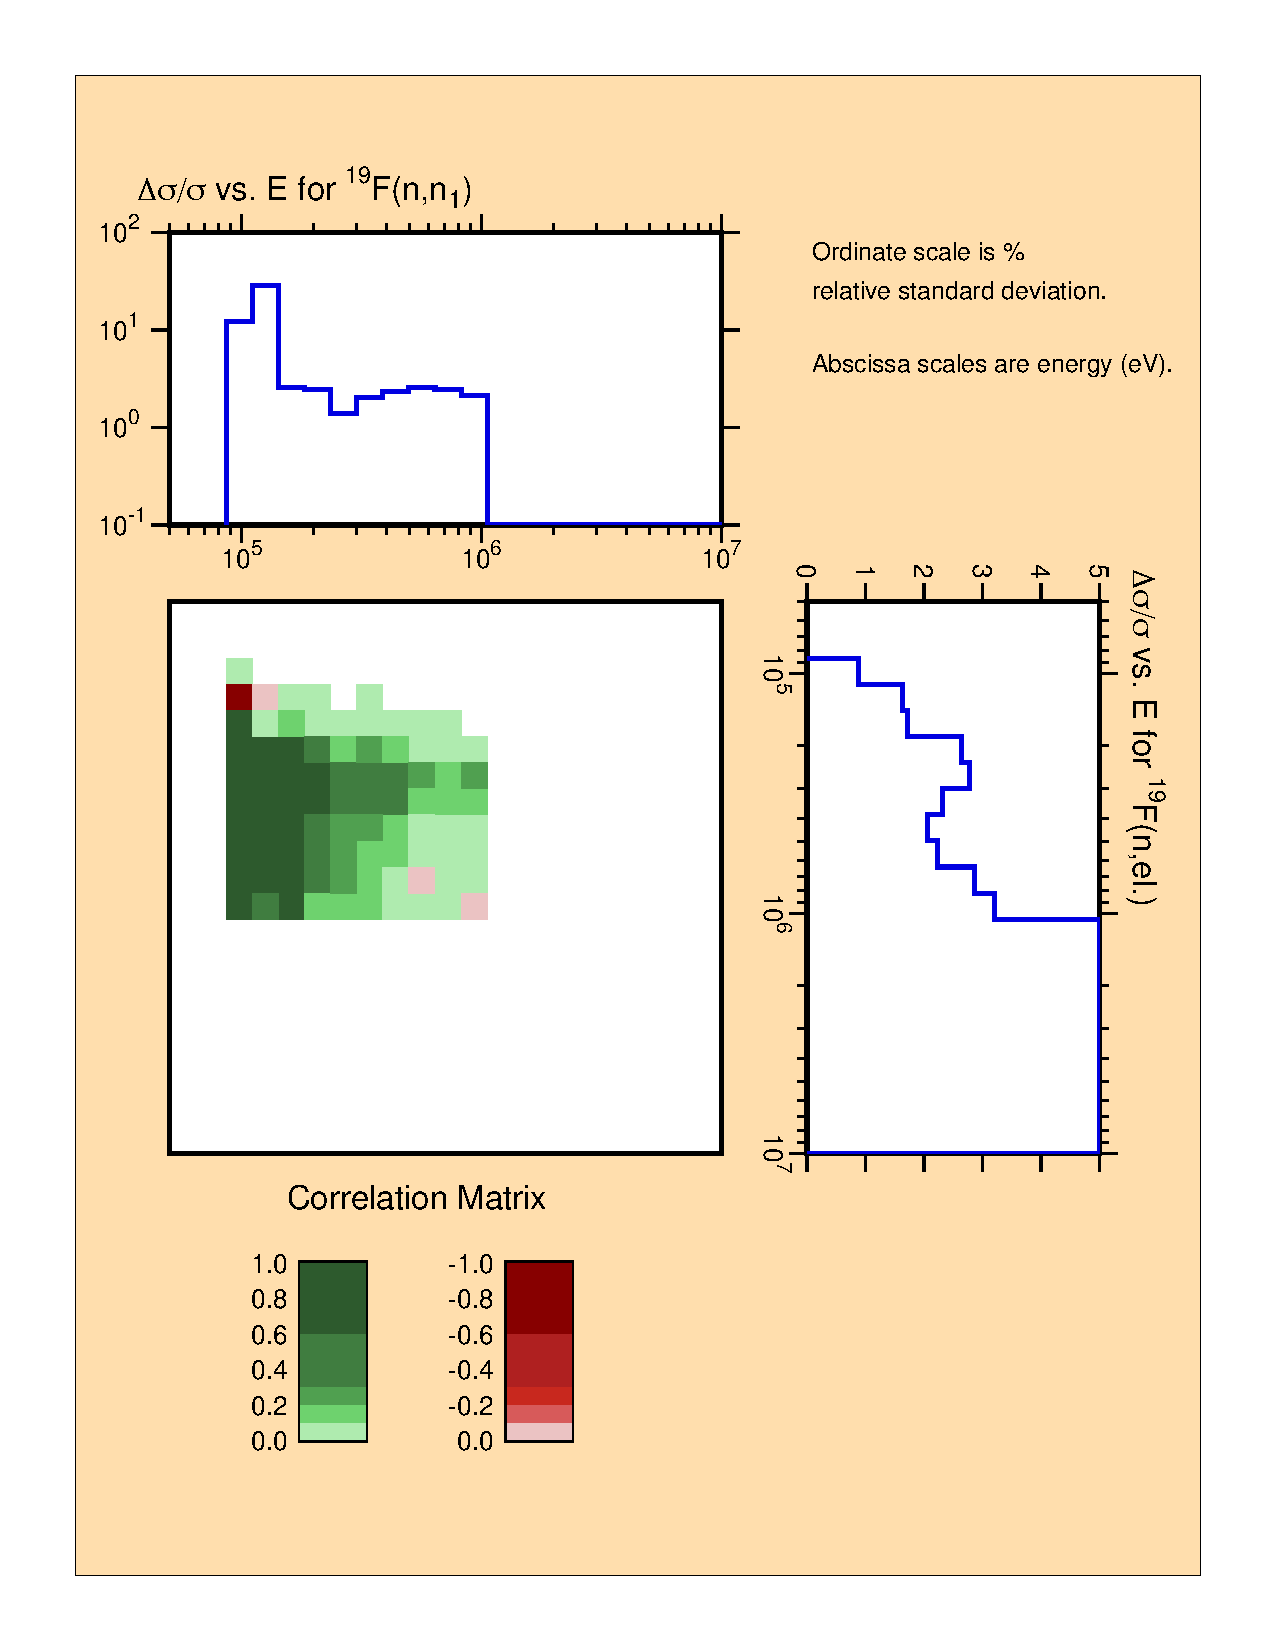
\includegraphics[keepaspectratio, width=5in,angle=0]{figs/covyyack}
\caption[Example of elastic scattering and (n,n$_1$) covariance data]
{Covariance plot for the elastic and (n,n$_1$) reactions from a
 sample ORNL evaluation for $^{19}$F, demonstrating the channel-channel
 covariances possible when using the Reich-Moore-Limited resonance
 representation.}
\label{covyy}
\end{figure}

\subsection{Secondary Particle Angular Distribution Covariances---File 34}
\label{ssERRORR_34}

File 34 contains covariances for angular distributions of secondary
particles.  While the underlying angular distribution data in File 4
may be given as tabulated distributions or as Legendre polynomial
coefficients, File 34's covariance data are only given for Legendre
coefficients.  At present there is no provision to specify covariances
between cross sections from File 3 and angular distributions from
File 4, nor to specify angular distribution covariances between
different materials.  The data format is governed by the \cword{LB}
flag discussed above in Section~\ref{ssERRORR_Str} with LB values
of 0, 1, 2, 5 and 6 allowed.

File 34 in the ENDF file may include covariance data for any MT
reaction defined in File 4, but currently NJOY only processes
the $P_1$ component of MT=2 (elastic scattering).

Fig.~\ref{mf34cov} shows an example of the covariances computed from File 34
for $^{238}$U from JENDL-3.3.  As usual, there are three components to this
plot.  On the right side, we illustrate $\bar{\mu}$ {\it vs} energy, which
dislays the expected forward-peaked characteristic with increasing energy;
on the top is
the uncertainty in $\bar{\mu}$ {\it vs} energy; and in the center is the
correlation matrix.   The ERRORR input for this case will be presented
below.

\begin{figure}[thb]\centering
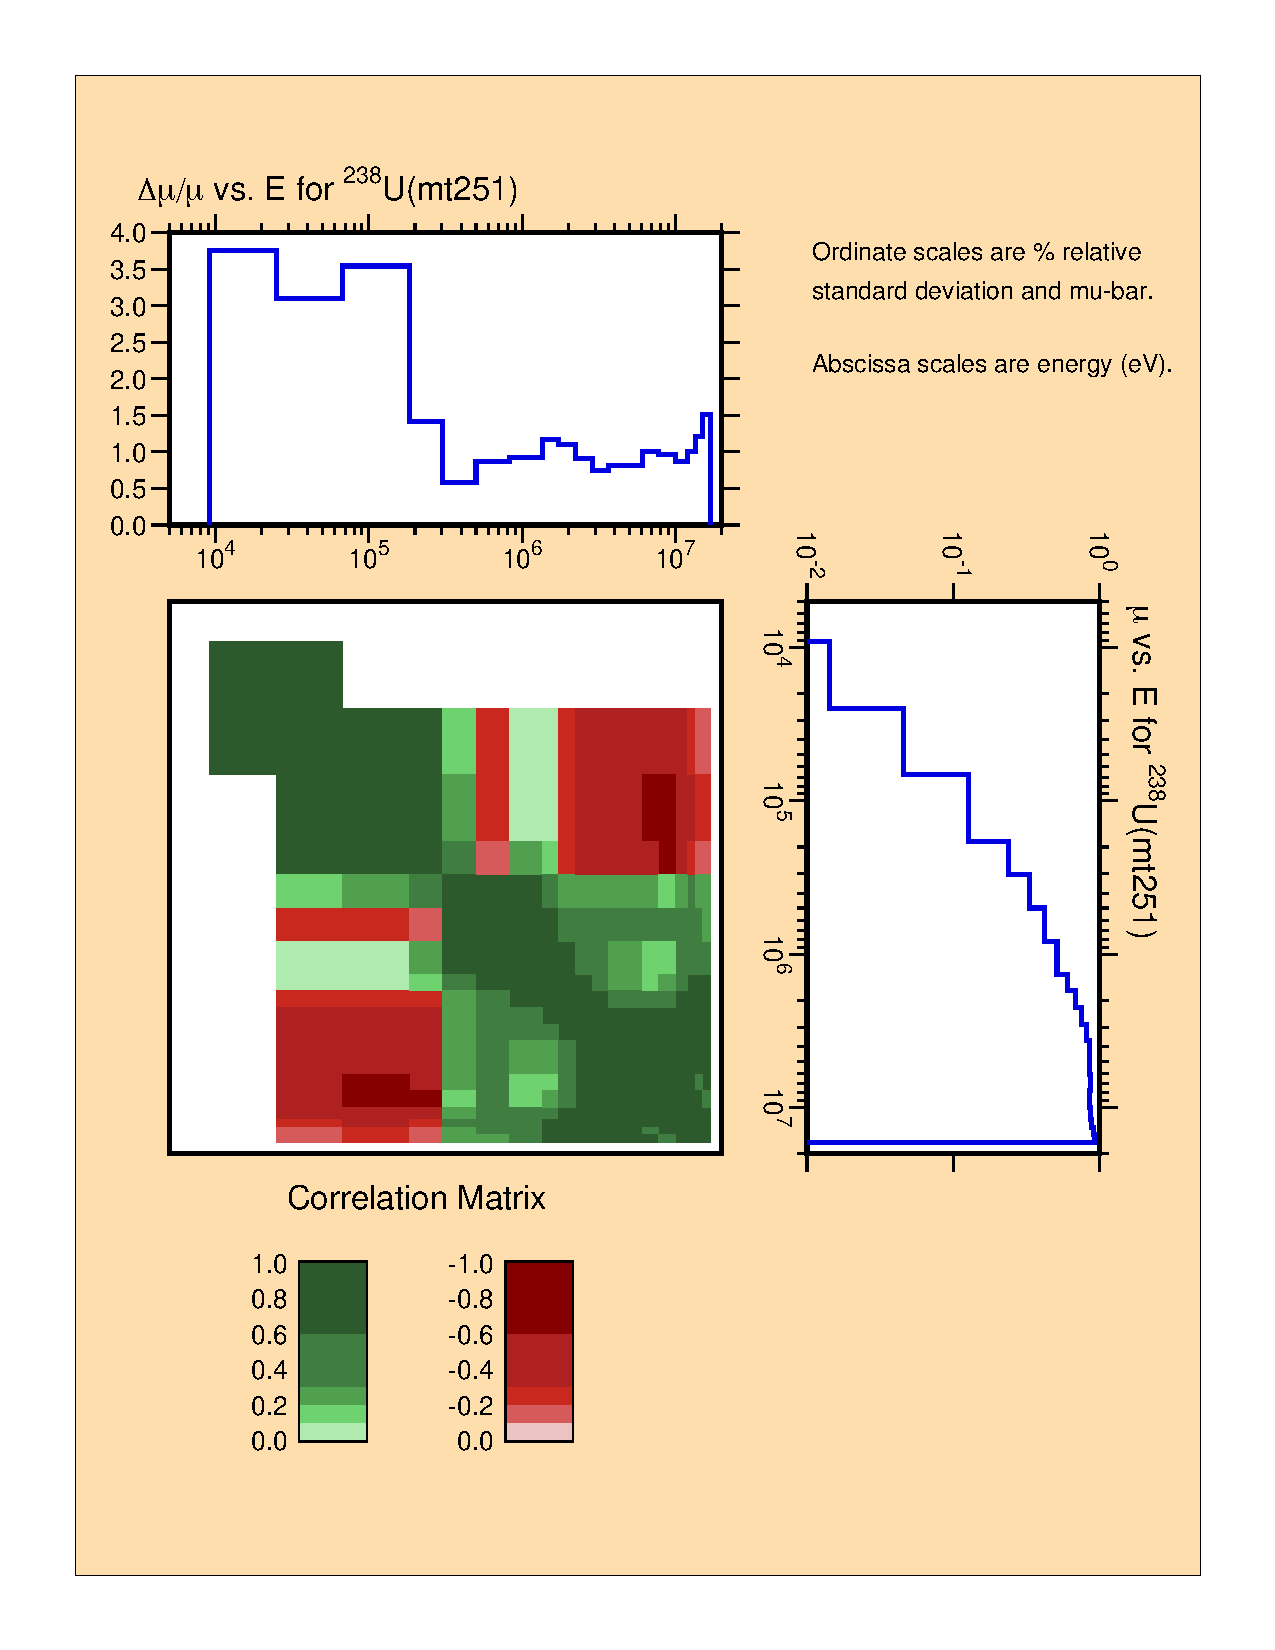
\includegraphics[keepaspectratio, width=5in, angle=0]{figs/mf34covack}
\caption[Example of angular distribution covariance data]{Example of angular
distribution covariance data.}
\label{mf34cov}
\end{figure}

\subsection{Secondary Particle Energy Distribution Covariances---File 35}
\label{ssERRORR_35}

File 35 contains covariance matrices for the energy distributions
of secondary particles given in File 5.  If the spectral distributions
are correlated with angular distributions and given in File 6, the
covariance information still appears in File 35 (the MT section
identifier is the common datum relating these data) and refers
to the angle-integrated distributions only.  The secondary energy
distribution is usually defined on a relatively fine energy grid,
and multiple distributions are given as a function of increasing
incident particle energy.  Since the uncertainties in secondary
distributions are usually highly correlated as a function of incident
particle energy, it is generally sufficient to only define a few
covariance matrices over relatively broad incident energy groups.
There is no provision to specify covariances between these groups
nor with data from other files such as File 3 cross sections or
File 1 prompt, delayed or total $\bar{\nu}$.

File 35 covariance data are given in a series of \cword{NK} subsections,
with each subsection covering a unique incident particle energy range.
The lowest energy of the first subsection and the highest energy of
the last subsection must cover the entire incident particle energy
range from File 5 (or File 6).  When processing MF35 data, the user
can specify the incident particle energy of interest (\cword{efmean}
on Card 7).  NJOY will process the \cword{NK}$^{\rm th}$ subsection whose
energy is closest to, but less than, \cword{efmean}.  The data
tabulated in the ENDF file are normalized probabilities of absolute
covariances identified as an \cword{LB}=7 subsection.  \cword{LB}=7
is identical to \cword{LB}=5 defined in Section~\ref{ssERRORR_Str}
except that these data are now absolute rather than relative covariances.

The ENDF format manual notes these matrices are probability distributions
that must remain normalized to unity and therefore the elements in these
symmetric matrices are constrained such that the sum of the elements
in any row (or column) must be zero.  This is sometimes referred to as
the ``zero sum" rule.  Of course, when dealing with real
numbers of finite precision whose values can vary by orders of magnitude
it is virtually impossible to rigorously conform to this rule.
Therefore, if the sum is sufficiently small, the rule is judged to be
satisfied.  If not, the ENDF manual provides a correction formula
to apply to all matrix elements.  When processing File 35 data NJOY,
checks this summation requirement and, if necessary, applies the
required correction.  NJOY uses the ``sufficiently small" criteria
specified in the Format manual for this check.

At present there are no File 35 data in ENDF/B-VII.0 neutron files,
but the $^{252}$Cf decay file does contain such data.  Also, these data
are becoming available in preliminary ENDF/B-VII.1 files available from
the National Nuclear Data Center (NNDC) at Brookhaven
National Laboratory (BNL).  These files follow
the ``zero sum' rule discussed above, but users are cautioned that
other internationally distributed files, particularly those from
JENDL-3.3, may provide File 35 data in an alternate format.  The
matrix elements in the JENDL-3.3 files have been divided by the
group energy width to yield energy-group averaged probability
distributions, as this is the data representation expected by the
Japanese ERRORJ code\cite{ERRORJ}\index{ERRORJ}.  A conversion code,
chmf35, has been developed and is available from the Nuclear Energy Agency
\footnote{chmf35 may be downloaded from
\href{http://www.nea.fr/dbprog/Njoy/chmf35.for}
{http://www.nea.fr/dbprog/Njoy/chmf35.for}}
to reformat these files
so that they are suitable for processing by NJOY.

Fig.~\ref{mf35cov}
shows the results of processing the ficticious $^{252}$Cf evaluation.  The
ERRORR input for this job will be presented below.

\begin{figure}[thb]\centering
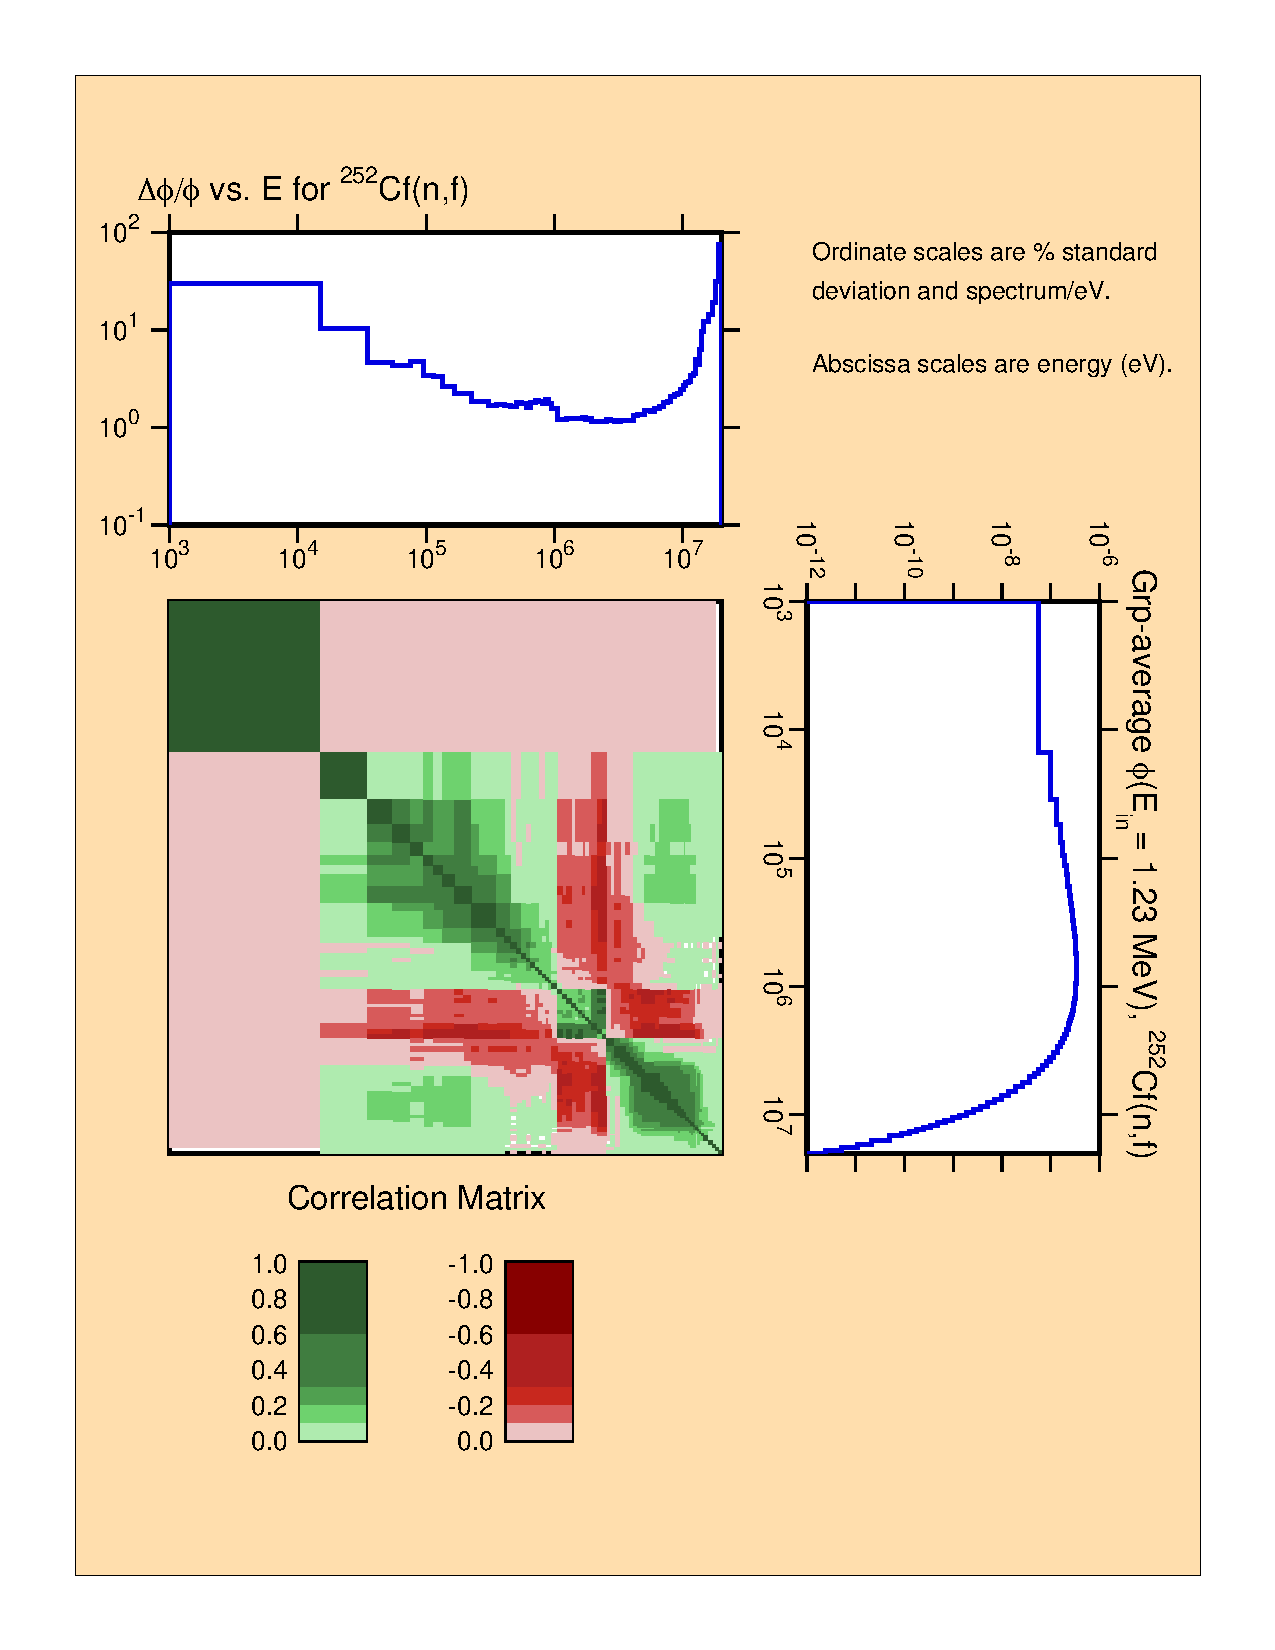
\includegraphics[keepaspectratio, width=5in, angle=0]{figs/mf35covack}
\caption[$^{252}$Cf(n,f) spontaneous fission spectrum covariance data]{Example
 of energy distribution covariances.  The appearance of negative correlations
 results from the requirement for preserving normalization.}
\label{mf35cov}
\end{figure}

\subsection{Radioactive Nuclide Production Covariances--File 40}
\label{ssERRORR_40}

There is only one file in ENDF/B-VII.0 that includes File 40 covariance
data -- $^{93}$Nb.  The input for calculating the $^{93m}$Nb production
uncertainty will be shown below, but the resulting covariances are shown
here in Fig.~\ref{mf40cov}.  The form of the graphical output
obtained when processing File 40 is identical to that produced when
processing File 33; with the cross section shown to the right, the
uncertainty shown to the top and the correlation matrix shown in the
center.  That these are File 40 data can be determined from the label
on the uncertainty portion of the plot.  In 2009, the File 40 format
was modified to include the \cword{IZAP} parameter that identifies the daughter
product.  We include this \cword{IZAP} value in the plot label so that the user
can more fully identify these data.  If an older File 40 file is processed
that does not define \cword{IZAP}, then the text string ``\cword{MF40}'' will
appear in the title.  In the example shown here we have modified the original
ENDF/B-VII.0 $^{93}$Nb file to include the proper \cword{IZAP} value in
File 40, which then appears in the plot title.

\begin{figure}[t]\centering
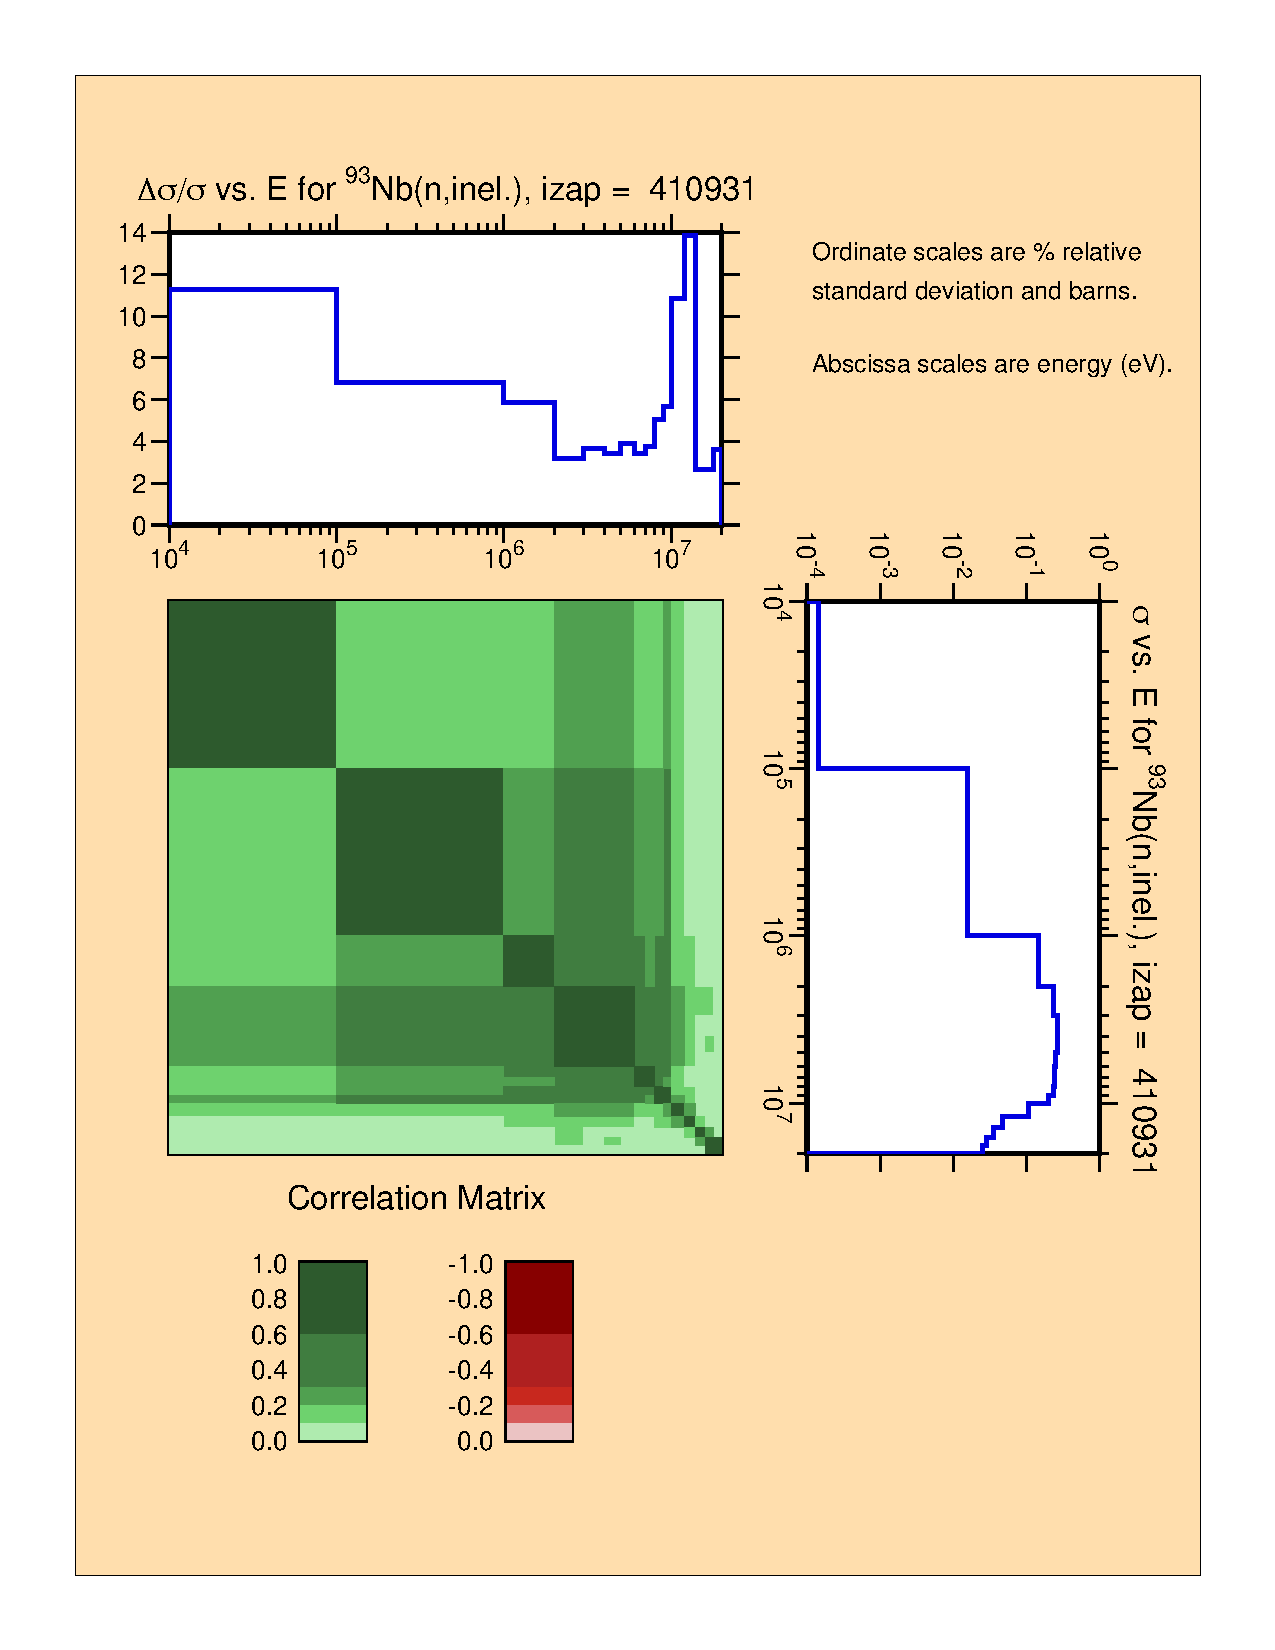
\includegraphics[keepaspectratio, width=5in, angle=0]{figs/mf40covack}
\caption[Radioactive nuclide production covariance example]{Example of
 radioactive nuclide production covariances.}
\label{mf40cov}
\end{figure}

\subsection{Calculation of Multigroup Fluxes, Cross Sections, and
 Covariances on the Union Grid}
\label{ssERRORR_UnionGrid}

As mentioned before, the main function of the ERRORR module is to
calculate the uncertainty in group-averaged cross sections at infinite
dilution due to uncertainty in the ENDF point data.  In this and the
following sections, we describe the procedures used in performing this
task.

In order to proceed, it is necessary to introduce into the discussion
three different energy grids, namely, the user grid, the ENDF grid, and
the union grid.  The relationship of these three grids is shown in
Fig.~\ref{grel}.  The user grid is the multigroup structure in which
the output multigroup covariances are to be produced.  The ENDF grid
is the collection of energies obtained (in subroutines
\cword{gridd}\index{gridd@{\ty gridd}} and
\cword{grist}\index{grist@{\ty grist}}) by forming
the union of (a) all energy ``lists'' appearing in any NI-type
sub-subsection of any subsection to be processed in the current ENDF
material, and (b) all energy pairs used to define the range of
effectiveness of any NC-type sub-subsection of any subsection to be
processed.  The union grid, on the other hand, is simply the union of
the user grid and ENDF grid.  The utility of the union grid is that (a)
the covariances are particularly simple to calculate in this grid, as
discussed below, and (b) the multigroup covariances needed by the user
are then easily obtained by a straightforward collapse from this to
the user grid.  In fact, the design of the current ENDF covariance
format was strongly influenced by the desire to employ this particular
procedure for multigroup processing\cite{Weisbin,Smith}.

\begin{figure}[b]\centering
$\begin{array}{lccccccccr}
{\rm User\; Grid} \; \;  &|&& \phi_1 , X_1  &  &|& & \phi_2 , X_2   &   &| \\
{\rm ENDF\; Grid} \; \;  &|& F_1 \; &|& &  F_2 & & |&  F_3               &| \\
{\rm Union \;Grid}  \; \;  &|&\phi_1 , x_1 &|& \phi_2 , x_1 &|&\phi_3 ,
   x_3 & | &\phi_4, x_4 &|\\
\end{array}$
\vspace{.25 in}
\caption{Illustration of energy grid relations.}
\label{grel}
\end{figure}

After the union grid is formed in subroutine
\cword{uniong}\index{uniong@{\ty uniong}}, the cross
sections $x(E)$ and weighting flux $\phi (E)$ are integrated to produce
$x_I$ and $\phi_I$, multigrouped on this grid.  If point cross sections
are supplied, an exact integration is done in subroutine
\cword{grpav}\index{grpav@{\ty grpav}}.  If, on the other hand, a
multigroup cross-section library is supplied, then subroutine
\cword{colaps}\index{colaps@{\ty colaps}} is used.  If a library group
is subdivided by a union-group boundary, then over the span of that
library group, the unknown energy dependencies of $x(E)$ and $\phi
(E)$, which are needed to calculate $x_I$ and $\phi_I $, are
approximated in subroutine \cword{colaps} by constants.  Normally, the
effect of this approximation is not large and, in any case, can be
reduced or eliminated by increasing the number of groups in the input
library.

We next consider the theoretical basis for the calculation of
union-grid multigroup covariances, as performed in subroutine
\cword{covcal}\index{covcal@{\ty covcal}}.  By definition, $x_I$
is just the average of $x(E)$ over union group I,

\begin{equation}
   x_I \; \equiv \;\frac  {\displaystyle\int_I \; \phi (E) \; x(E) \;
  dE}{\displaystyle\int_I \; \phi (E) \; dE} \,\,,
\label{e19}
\end{equation}

\noindent
where $\phi (E)$ is the flux ``model'' assumed for the multigroup
calculations.  Let $y_J$ denote similarly the average of $y(E)$ over
union group $J$.

Let us imagine that these groups are subdivided into many subintervals
of infinitesimal width, so that in the i$^{\rm{th}}$ subinterval of group I,
for example, $x(E)$ can be well approximated by the constant $x_i$.  By
this device, the integrals that define $x_I$ and $y_J$ can be converted
to discrete sums:

\begin{equation}
x_I \; = \frac{{\displaystyle \sum_{i\in I}} \; \phi_i \; x_i}{\phi_I } \; = \;
\sum_{i\in I} \; \alpha_{Ii} \; x_i\,\,,
\label{e20}
\end{equation}

\noindent
where

\begin{eqnarray}
\phi_i & = & \int_{i} \; \phi (E) \; dE \;,\\
\nonumber \\
\phi_I & = & \sum_{i\in I} \; \phi_{i} \; = \; \int_{I} \; \phi (E) \; dE\;,
\end{eqnarray}

\noindent
and

\begin{equation}
\alpha_{Ii} \equiv \frac{\phi_i}{\phi_I} \; .
\end{equation}

\noindent
From these definitions, clearly

\begin {equation}
\sum_{i\in I}\; \alpha_{Ii} \; = \; 1 \; .
\label{e24}
\end{equation}

\noindent
Similarly for $y$,

\begin{equation}
y_J = \sum_{j\in J} \; \alpha_{Jj} \; y_j\;,
\label{e25}
\end{equation}

\noindent
and

\begin{equation}
\sum_{j \in J} \; \alpha_{Jj} = 1 \;.
\label{e26}
\end{equation}

The methodology of ERRORR assumes that $\phi(E)$ in Eq.~\ref{e19} is
free of uncertainty.  Under this assumption, the terms $\alpha_{Ii}$
and $\alpha_{Jj}$ are simply known constants.  The covariance of $x_I$
with $y_J$ can then be calculated using the propagation-of-errors
formula, Eq.~\ref{e11}, together with Eqs.~\ref{e20} and \ref{e25}.

\begin{eqnarray}
{\rm {\rm cov}} (x_I,y_J) & = & \sum_{i\in I\atop{j\in J}}\;
  \alpha_{Ii} \; \alpha_{Jj} \; {\rm cov}
 (x_i ,y_j) \nonumber \\
\nonumber \\
 & = & \sum_{i\in I\atop{j\in J}}\; \alpha_{Ii} \; \alpha_{Jj} \; \sum_{n}{\rm
 cov} (x_i ,y_j)_n \; ,
\end{eqnarray}

\noindent
where the summation over $n$ results from the different independent
contributions to the ENDF point covariances coming from the different
NI-type sub-subsections.  Changing the order of summation, we obtain

\begin{equation}
{\rm  cov} (x_I,y_J) \; = \; \sum_{n} \; {\rm cov} (x_I,y_J)_n \; ,
\label{e28}
\end{equation}

\noindent
where
\begin{equation}
{\rm cov} (x_I,y_J)_n \;=\; \sum_{i\in I\atop{j\in J}} \; \alpha_{Ii}\;
\alpha_{Jj}\;\; {\rm {\rm cov}} (x_i,y_j)_n \; .
\label{e29}
\end{equation}

To evaluate the sum in Eq.~\ref{e29}, we make use of the fact that union
groups {\it I} and {\it J} do not cross any ENDF grid boundaries.
Recalling the discussion of NI-type sub-subsections (and
excluding for the moment the case where sub-subsections with
\cword{LB}=8 are present), there are only two possibilities for the
energy dependence of the covariance between ENDF grid points; thus,
over the limits of the sum, either cov$(x_i,y_j)_n$ is independent of
$i$ and $j$ (if \cword{LB}=0) or rcov$(x_i,y_j)_n$ is independent of
$i$ and $j$ (if $1\leq$ \cword{LB} $\leq 6$).  We consider first the
constant-absolute-covariance case, \cword{LB}=0.  Eq.~\ref{e29} can then be
rewritten as follows:

\begin{equation} {\rm {\rm cov}} (x_I,y_J)_n\; = \; {\rm {\rm cov}} (x,y)_n
\; \sum_{i\in I\atop{j\in J}} \; \alpha_{Ii} \; \alpha_{Jj} \; = \;
  {\rm {\rm cov}} (x,y)_n
\left(\sum_{i\in I} \; \alpha_{Ii} \right) \left(\sum_{j\in J} \;
  \alpha_{Jj}\right) \; .
\end{equation}

\noindent
Invoking Eqs.~\ref{e24} and \ref{e26}, we obtain

\begin{equation}
{\rm cov}(x_I , y_J)_n \;=\; {\rm cov}(x,y)_n \; \;\;\;\;\;
  (\hbox{\cword{LB}} = 0) \;.
\label{e31}
\end{equation}

\noindent
For \cword{LB}-values ranging from 1 to 6, the relative covariance is
constant over each union group, so we rewrite Eq.~\ref{e29} in the form

\begin{eqnarray}
{\rm {\rm cov}} (x_I,y_J)_n & = & \sum_{i\in I\atop{j\in J}}\; \alpha_{Ii}\;
  \alpha_{Jj} \; x_i \; x_j \;
{\rm r{\rm cov}} (x_i , x_j)_n \nonumber \\
  & = &{\rm r{\rm cov}} (x,y)_n \sum_{i\in I\atop{j\in J}}\;
 (\alpha_{Ii}\; x_i ) \; (\alpha_{Jj} \; y_j) \nonumber \\
  & = & {\rm rcov} (x,y)_n \; \left(\sum_{i\in I} \; \alpha_{Ii} \;
  x_i \right) \left(\sum_{j\in J}\; \alpha_{Jj} \; y_j \right) \; .
\label{e32}
\end{eqnarray}

\noindent
Substituting here from Eqs.~\ref{e20} and \ref{e25}, we obtain

\begin{equation}
{\rm {\rm cov}} (x_I , y_J)_n = x_I\; y_J \; {\rm r{\rm cov}} (x,y)_n
  \;\;\;\;\;\; (1
\leq\hbox{\cword{LB}}\leq 6)\; .
\label{e33}
\end{equation}

\noindent
The final union-group multigroup covariance is obtained by inserting
these results, Eqs.~\ref{e31} and \ref{e33}, back into Eq.~\ref{e28}

\begin{equation} {\rm cov} (x_I,y_J) = \; \sum_{\rm n(LB=0)}  \;
{\rm cov} (x,y)_n \;+\; \sum_{\rm  n(LB=1,6)}  \;x_I\;y_J
\; {\rm r{\rm cov}} (x,y)_n\;,
\label{e34}
\end{equation}
\vspace{1 pt}

\noindent
where the first sum runs over all sub-subsections with \cword{LB}=0 and
the second runs over all sub-subsections with \cword{LB}=1 through 6.  The
quantities cov$(x,y)_n$ and r{\rm cov}$(x,y)_n$ here
are simply the point-energy covariances from the ENDF covariance file,
as described in Eqs.~\ref{e12} through \ref{lbopts}.  Equation \ref{e34}
then is the basic equation used in subroutine \cword{covcal} to
calculate the desired union-group covariances.

The final step, if sub-subsections with \cword{LB}=8 are present, is to
increment the diagonal elements (variances) as follows:

\begin{equation}
{\rm cov} (x_I, x_I) = {\rm cov} (x_I, x_I) +
F_k\,(E_{k+1} - E_k)/\Delta E_I \;,
\label{e35}
\end{equation}

\noindent
where k indexes the range of the \cword{LB}=8 energy grid that includes
union group {\it I}.

\subsection{Basic Strategy for Collapse to the User Grid}
\label{ssERRORR_GridStrategy}

The union-group fluxes $\phi_I$ are used, in subroutine
\cword{sigc}\index{sigc@{\ty sigc}}, to collapse the union-group
cross sections to the coarser user grid.  Changing notation slightly,
let us denote by $x_I(a)$ the cross section in union group {\it I}
for reaction $a$, and similarly let $X_K (a)$ be the cross section
in user group {\it K} for the same reaction.  In complete analogy
with Eq.~\ref{e20},

\begin{equation}
X_K(a) = \frac {\displaystyle{\sum_{I\in K}\; \phi_I\;x_I(a)}}{\phi_K}
 \;=\; \sum_{I\in K} \; A_{KI} \; x_I(a)\;,
\end{equation}

\noindent
where

\begin{equation}
\phi_K = \sum_{I\in K} \;\phi_I \;,
\end{equation}

\noindent
and

\begin{equation}
A_{KI} = \frac{\phi_I}{\phi_K}\;.
\end{equation}

\noindent
Applying the propagation-of-errors formula again gives

\begin{equation}
{\rm cov} \left[X_K(a),X_L(b) \right] = \sum_{I\in K\atop{J\in L}}\;
  A_{KI}\;A_{LJ}\;{\rm {\rm cov}}[x_I(a),x_J(b)] \;.
\label{e39}
\end{equation}

\noindent
An alternative expression, obtained by simply rearranging coefficients, is

\begin{equation}
{\rm {\rm cov}} \left[X_K(a),X_L(b) \right] =
  \frac{1}{\phi_K \phi_L} \sum_{I\in K\atop{J\in L}} \; T_{IJ}(a,b) \; ,
\label{e40}
\end{equation}

\noindent
where

\begin{equation}
T_{IJ}(a,b) = \phi_I\;\phi_J \; {\rm cov} [x_I(a),x_J(b)]\;.
\label{e41}
\end{equation}
\vspace{1 pt}

\noindent
Eqs.~\ref{e40} and \ref{e41} provide the basic framework in the ERRORR
module for the production of multigroup covariances in the coarse user-group
structure.  Finally, if requested, the Eq.~\ref{e40} absolute covariances
are converted to relative form,

\begin{equation}
{\rm r{\rm cov}} [X_K(a),X_L(b)] =
  \frac{{\rm cov} [X_K(a),X_L(b)]}{X_K(a)\;X_L(b)} \;.
\label{e42}
\end{equation}

\subsection{Group-Collapse Strategy for Data Derived by Summation}
\label{ssERRORR_summ}

The procedure described in the previous section must be modified if, in
some energy range, either reaction $a$ or $b$ is a ``derived'' quantity
in the sense of Eq.~\ref{e17} or Eq.~\ref{e18}.  In such a case, one
cannot apply Eq.~\ref{e34} directly to the calculation of
${\rm {\rm cov}}[x_I (a),x_J(b)]$, because the covariances on the
right-hand side of Eq.~\ref{e34} will be missing from the ENDF file in
the affected energy region.

We consider first the case in which some cross sections are evaluated
(``derived'') by simply summing other evaluated cross sections, as in
Eq.~\ref{e17}.  Equation \ref{e35} can then be rewritten as

\begin{equation}
X_K(a) = \sum_{I\in K} \; A_{KI} \;\left\{\sum_{{\rm all\; c}} \;
  C_I(a,c)\;x_I(c)\right\} \;,
\end{equation}

\noindent
where the quantity in curly brackets is the value of the derived cross
section ``a'' in union group {\it I}, as reconstructed from the
directly evaluated cross sections $x_I (c)$.  The derivation
coefficients $C_I (a,c)$ depend on the union-group index {\it I},
because the evaluator is permitted to employ different derivation
strategies in different energy ranges in order to simplify and shorten
the covariance files.

To expand on this last point, suppose there are only three reactions,
and suppose that the cross sections $x(1)$ and $x(2)$ rigorously sum to
$x(3)$ at all energies.  Further suppose that within the
energy range {\rm cov}ered by the first union group, the cross-section
evaluator has used this logical connection in order to ``derive''
$x(3)$, that is to evaluate $x(3)$, by summing the existing evaluations
for $x(1)$ and $x(2)$,

\begin{equation}
x_1(3) = x_1(1)\;+\;x_1(2)\;.
\end{equation}

\noindent
Further suppose that in the range of union group 2, $x(1)$ is derived by
employing the same logical connection, but in a different way,

\begin{equation}
x_2(1) = x_2(3)-x_2(2)\;,
\end{equation}

\noindent
and in union group 3, all three reactions are directly evaluated.

In this example $C_I(a,c)$ has the following values:
\begin{center}
$\begin{array}{lll}

\makebox[1.25in]{
$\begin{array}{llr}
C_1(1,1) & = & 1 \\
C_1(2,1) & = & 0\\
C_1(3,1) & = & 1
\end{array}$}
&
\makebox[1.25in][l]{
$\begin{array}{llr}
C_1(1,2) & = & 0 \\
C_1(2,2) & = & 1 \\
C_1(3,2) & = & 1
\end{array}$}
&
\framebox[1.25in]{
$\begin{array}{llr}
C_1(1,3) & = & 0 \\
C_1(2,3) &= & 0 \\
C_1(3,3) & = & 0
\end{array}$}
\\
\\
\framebox[1.25in]{
$\begin{array}{llr}
C_2(1,1) & = & 0 \\
C_2(2,1) & = & 0 \\
C_2(3,1) & = & 0 \\
\end{array}$}
&
\makebox[1.25in][l]{
$\begin{array}{llr}
C_2(1,2) & = & -1 \\
C_2(2,2) & = & 1 \\
C_2(3,2) & = & 0
\end{array}$}
&
\makebox[1.25in]{
$\begin{array}{llr}
C_2(1,3) & = & 1 \\
C_2(2,3) & = & 0 \\
C_3(3,3) & = & 1
\end{array}$}
\\
\\
\makebox[1.25in]{
$\begin{array}{llr}
C_3(1,1) & = & 1 \\
C_3(2,1) & = & 0 \\
C_3(3,1) & = & 0
\end{array}$}
&
\makebox[1.25in][l]{
$\begin{array}{llr}
C_3(1,2) & = & 0 \\
C_3(2,2) & = & 1 \\
C_3(3,2) & = & 0
\end{array}$}
&
\makebox[1.25in]{
$\begin{array}{llr}
C_3(1,3) & = & 0 \\
C_3(2,3) & = & 0 \\
C_3(3,3) & = & 1
\end{array}$}
\end{array}$
\end{center}

\noindent
Note that in all cases we have formally considered the evaluated cross
sections to be derived from themselves, $C_I(a,c)|_{\rm eval}{=}
\delta_{ac}$.  This device allows us to use Eq.~\ref{e42} for all
reactions, regardless of whether they are derived or
evaluated.  Note that, in every case where reaction $c$ is
derived in group $I,\; C_I(a,c) {=} 0$.  (See boxed submatrices.)
This null ``sensitivity coefficient'' is important, because it means
that Eq.~\ref{e42} remains a linear relation involving only dependent
quantities with known covariances (the evaluated subset
of the union-group cross sections) on the right.  This allows us once
again to use the propagation-of-errors formula to obtain the desired
user-group covariances.

\begin{equation}
{\rm cov} [X_K,(a),X_L(b)] = \sum_{{\rm all \; c\;} \atop{\rm all \;d\;}}
 \sum_{I\in K\atop {J \in L}} \; A_{KI} \; C_I (a,c) \; A_{LJ} \;
   C_J (b,d) \; {\rm {\rm cov}} [x_I(c),x_J(d)]\; ,
\label{e46}
\end{equation}

\noindent
or, alternatively,

\begin{equation}
{\rm {\rm cov}} [X_K,(a),X_L(b)] = \frac{1}{\phi_K \phi_L}\;
  \sum_{{\rm all \; c\;} \atop{\rm all \;d\;}}
 \sum_{I\in K\atop {J \in L}} \; C_I(a,c)\; C_J(b,d) \; T_{IJ}(c,d)\; ,
\end{equation}

\noindent
where
\begin{equation}
T_{IJ}(c,d) = \phi_I\; \phi_J \; {\rm {\rm cov}} [x_I(c),x_J(d) ] \; .
\end{equation}

In subroutine \cword{covcal}\index{covcal@{\ty covcal}}, the
flux-covariance product $T_{IJ}$ is calculated for all evaluated
reaction pairs and written to a ``scratch'' binary disk file, unit 11.
 (For diagnostic purposes, it is possible to change this to a
formatted scratch file by manually resetting the variable
\cword{imode} to  $+1$ in the main program.)  In
the subsequent collapse to the user's group structure in
subroutine \cword{covout}, the user-group covariances ${\rm {\rm
cov}}[X_K(a),X_L(b)]$ for one specific a-b reaction pair, for all
``\cword{MT1}'' energy groups L, and for as large a range of ``\cword{MT}''
energy groups K as possible, are calculated simultaneously in memory.

In \cword{covout}\index{covout@{\ty covout}}, the disk file (unit 11)
is rewound and read completely through, once in each range of MT groups
for each a-b reaction pair, to access the union-group covariances for
the evaluated reactions.  As the union-group data pass through memory,
contributions to the user-group covariances are accumulated using
Eq.~\ref{e46}.

In the fairly common situation where cross sections $x(a)$ and $x(b)$
are directly evaluated over the whole energy range of the data
file,

\begin{equation}
C_I(a,c) = \delta_{ac},\; {\rm for \; all} \; I,
\end{equation}

\noindent
and

\begin{equation}
C_J(b,d) = \delta_{bd},\; {\rm for \; all} \; J.
\end{equation}

\noindent
In this case, Eq.~\ref{e46} can be greatly simplified.

\begin{eqnarray}
  {\rm {\rm cov}} [X_K(a),X_L(b)] & =
  & \frac{1}{\phi_K \phi_L}\;\sum_{{\rm all \; c\;}
  \atop{\rm all \;d\;}}
  \sum_{I\in K\atop {J \in L}} \;\delta_{ac} \; \delta_{bd} \;
  T_{IJ} (c,d)  \nonumber \\ & = &
  \frac{1}{\phi_K \phi_L} \sum_{I\in K\atop {J \in L}} \;
  T_{IJ} (a,b) \; .
\end{eqnarray}

This result, which is identical to Eq.~\ref{e39}, suggests a shortcut
calculational path, which is followed in subroutine
\cword{covout}\index{covout@{\ty covout}} whenever both reactions
are directly evaluated.  In preparation for this situation, a second
copy of the \cword{covcal}\index{covcal@{\ty covcal}} binary output file
is generated when \cword{covout} is first called.  The second copy, on
unit 12, is read only in the trivial derivation cases just described
(flagged in the code by setting \cword{isd}=1).  Unit 12 is not rewound
before processing a given reaction pair a-b, since earlier reaction
pairs on the file do not contribute to the sum in Eq.~\ref{e46} in these
cases.  Reading of the second copy stops after the union-group
covariances for reaction pair a-b are found, because the later reaction
pairs do not contribute either.


\subsection{Processing of Data Derived from Ratio Measurements}
\label{ssERRORR_Ratio}

The treatment of implicit covariances that arise from ratio
measurements, as in Eq.~\ref{e18}, is totally different from the treatment
of data derived by summation, Eq.~\ref{e17}, discussed in the previous
section.  Before discussing the processing details, it is helpful first
to review the subject of ratio evaluations generally.  Returning to the
``x-y'' notation of Section~\ref{ssERRORR_Defs}, let $x(E_x)$ be the
value of the cross
section for reaction $x$ at energy $E_x$, and $y(E_y)$ the cross
section for reaction $y$ at energy $E_y$.  In some energy region
$(L_x,H_x)$, suppose that the best knowledge of $x(E_x)$ is obtained
through the application of a measured ratio, $u(E_x)$:

\begin{equation}
x(E_x) = u(E_x) \; z(E_x), \;{\rm if} \; L_x \leq E_x \leq H_x \; ,
\end{equation}

\noindent
where reaction $z$ is some well-known cross section,
possibly one of the official ENDF/B standard cross sections.
Similarly, suppose $y$ is derived from the same standard, over a
possibly different energy range:

\begin{equation}
y(E_y) = v(E_y) \; z(E_y), \;{\rm if} \; L_y \leq E_y \leq H_y \; .
\end{equation}

\noindent
By performing a first-order Taylor-series expansion and then applying
the formula for propagation of errors, one can obtain an expression for the
contribution to the relative covariance, ${\rm r{\rm
cov}}[x(E_x),y(E_y)],$ that is attributable to these ratio measurements.
In the usual case, where the ratios $u$ and $v$ are only weakly
correlated with the standard cross section $z$, the result is quite
simple:

\begin{equation}
{\rm rcov}[x(E_x),y(E_y)]_{{\rm ratio}} = {\rm rcov}[u(E_x),v(E_y)] +
 {\rm rcov}[z(E_x),z(E_y)]
\end{equation}

\noindent
if $L_x \leq E_x \leq H_x$ and $L_y \leq E_y \leq H_y$, and

\begin{equation}
{\rm rcov} [x(E_x), y(E_y)]_{\rm ratio}= 0 \;\;{\rm otherwise}.
\label{e55}
\end{equation}

\noindent
Thus, in this fairly common evaluation situation, the covariance
separates naturally into a part involving only the measured ratios and
a part involving only the standard.  Because the second contribution,
cov(MT$_z$, MT$_z$), can be read directly from the NI-type
sub-subsections in evaluation for the standard, it is not included
explicitly in the ENDF subsections for the derived quantities,
cov(MT$_x$, MT$_x$) or cov(MT$_y$, MT$_y$).  Instead, the existence of
this additional contribution to the covariance is signalled by the
presence of an NC-type sub-subsection.

The strategy adopted for processing this information in
subroutine \cword{stand}\index{stand@{\ty stand}} is to load the
NI-type sub-subsections from the evaluation of the standard into
the same storage array that is used to store NI-type covariances
from the evaluation for reaction $x$.  From that point on, the data
from the standard are handled just as if they had come from the
evaluation for $x$, but with one exception.  As indicated by
Eq.~\ref{e55}, the covariance contribution
${\rm {\rm cov}}[z(E_x),z(E_y)]$ is \underline{not} added into
the total covariance matrix for the current reaction pair if
either $E_x$ or $E_y$ lies outside the corresponding energy
``window'' $(L_x,H_x)$ or $(L_y,H_y)$, respectively.

As discussed in Section~\ref{ssERRORR_Str}, in addition to identifying
the standard reaction, the NC-type sub-subsection contains a control parameter
\cword{LTY} and two energies \cword{EL} and \cword{EH} whose
significance depends on \cword{LTY}.   ~\cword{LTY} is used to identify
particular evaluation scenarios: reaction $x$ is the same as reaction
$y$ (or at least they are derived from $z$ over the same energy range)
(\cword{LTY}=1); $y$ is identical to the standard (\cword{LTY}=2); or
$x$ is identical to the standard (\cword{LTY}=3).  A fourth
possibility, namely, that $x$, $y$, and $z$ are entirely distinct,
cannot presently be treated with a single NC-type sub-subsection; that
is, there is no \cword{LTY} value defined for this case.  However, as
discussed later, it is still possible to process covariances for this
situation by combining information from sub-subsections in two
different evaluations.  For convenience, we shall refer to this fourth
case as \cword{LTY}=4.

The interrelationship of \cword{LTY}, \cword{EL}, \cword{EH}, and the
windows $(L_x,H_x)$ and $(L_y,H_y)$ used in ERRORR for the
``zeroing-out'' operation of Eq.~\ref{e55}, is summarized below:

\small
\begin{eqnarray}
\mathtt{LTY=1}  \nonumber \\
   &   & (L_x, H_x) = (L_y, H_y) = (\mathtt{EL},\mathtt{EH}) \nonumber \\
\mathtt{LTY=2} \nonumber \\
   &   & (L_x, H_x) =  (\mathtt{EL},\mathtt{EH}) \nonumber \\
   &   & (L_y, H_y) = (10^{-5} \;{\rm eV},\; 20 \;{\rm MeV}) \nonumber \\
\mathtt{LTY=3} \nonumber \\
   &   & (L_x, H_x) = (10^{-5}\; {\rm eV},\; 20 \; {\rm MeV}) \nonumber \\
   &   & (L_y, H_y) =  (\mathtt{EL},\mathtt{EH}) \nonumber \\
\mathtt{LTY=4} \nonumber \\
   &   & (L_x, H_x) =  (\mathtt{EL},\mathtt{EH}) \nonumber \\
   &   & (L_y, H_y) =  (\mathtt{EL'},\mathtt{EH'}) \; .
\end{eqnarray}
\normalsize

\noindent
If the user requests covariance data, ${\rm {\rm cov}}(x,y)$, where $x$
and $y$ are different and both are distinct from the standard
(\cword{LTY}=4), the ERRORR module obtains (\cword{EL,EH}) from the
\cword{LTY}=2 subsection in the evaluation for $x$ that ``points'' to
$z$.  Then, the covariance file for $z$ is read to obtain both (a) the
explicit covariances ${\rm {\rm cov}}(z,z)$ and (b) the second energy
window (\cword{EL}$'$, \cword{EH}$'$), the latter being found in the
\cword{LTY}=3 sub-subsection that points back to $y$.

We will illustrate ratio covariance processing using data from ENDF/B-V.
Table~\ref{ratios} lists all ENDF/B-V reactions that contain ratio-to-standard
covariance data.  The symbols entered in the reaction-by-reaction
matrix indicate which reactions are referenced as standards ($\ast$),
and which reaction pairs have implicit nonzero covariances
(\cword{LTY}).  ERRORR will produce multigroup covariances for any of
the reaction pairs in Table~\ref{ratios} that are marked with ($\ast$) or
(\cword{LTY}).  The cross-material covariances (\cword{LTY}=2, 3, or 4)
must be requested individually using the
\cword{IREAD}=2 option (see Section~\ref{ssERRORR_inp}, especially
the discussion of
Cards 10 and 11).  An attempt to process covariances for any of the
cases \cword{LTY}=1 through 4 without supplying a separate ENDF
tape containing the needed standard will result in an error stop in
subroutine \cword{gridd}.  The error diagnostic, however, will supply
the details of the corrective action required.  (See general discussion
of diagnostic messages in Section~\ref{ssERRORR_msg}.)

\begin{table}
\caption{Covariance Matrices Affected by Ratio
 Measurements In ENDF/B-V}
\label{ratios}
\setlength{\extrarowheight}{1pt}
\begin{center}
\begin{tabular}{lccccccc}
\hline
    & $^{10}$B & $^{238}$U & $^{235}$U & $^{239}$Pu & $^{239}$Pu
        & $^{241}$Am & $^{242}$Pu \\
  & (n,$\alpha$) & (n,$\gamma$) & (n,f) & (n,f) & (n,$\gamma$)
      & (n,f) & (n,f) \\ \hline
$^{10}$B(n,$\alpha$) & $\ast$ & 3 \\
$^{238}$U(n,$\gamma$) & 2 & 1 \\
$^{235}$U(n,f) &   &   & $\ast$ & 3 & 3 & 3 & 3 \\
$^{239}$Pu(n,f) &  &  & 2 & 1 & 1 & 4 & 4 \\
$^{239}$Pu(n,$\gamma$) &  &  & 2 & 1 & 1 & 4 & 4 \\
$^{241}$Am(n,f) &  &  & 2 & 4 & 4 & 1 & 4 \\
$^{242}$Pu(n,f) &  &  & 2 & 4 & 4 & 4 & 1 \\  \hline
\end{tabular}
\end{center}
\hspace{10mm}
\begin{minipage}{3in}
$\ast = $ standard \\
Integer $=$ \cword{LTY} value (see text)
\end{minipage}
\end{table}

As an example of the ratio-data capabilities of ERRORR,  Fig.~\ref{ratcov}
shows the covariances between the fission cross sections of $^{239}$Pu
(reaction $x$) and those of the important actinide $^{241}$Am (reaction
$y$).  This is an \cword{LTY}=4 case where $(L_x, H_x){=}$ $(0.2 \;{\rm
MeV}, 15 \;{\rm MeV})$ and $(L_y, H_y){=}(0.2 \;{\rm MeV}, 20 \; {\rm
MeV})$.  The effect of using two different windows is apparent in
the lower right corner of the correlation matrix.  The plot itself was
produced with NJOY's \hyperlink{sCOVRhy}{COVR}\index{COVR}
module.  The complete input needed to compute and plot these data is
given below (see the fourth input example in Section~\ref{ssERRORR_inp}).

\begin{figure}[t]\centering
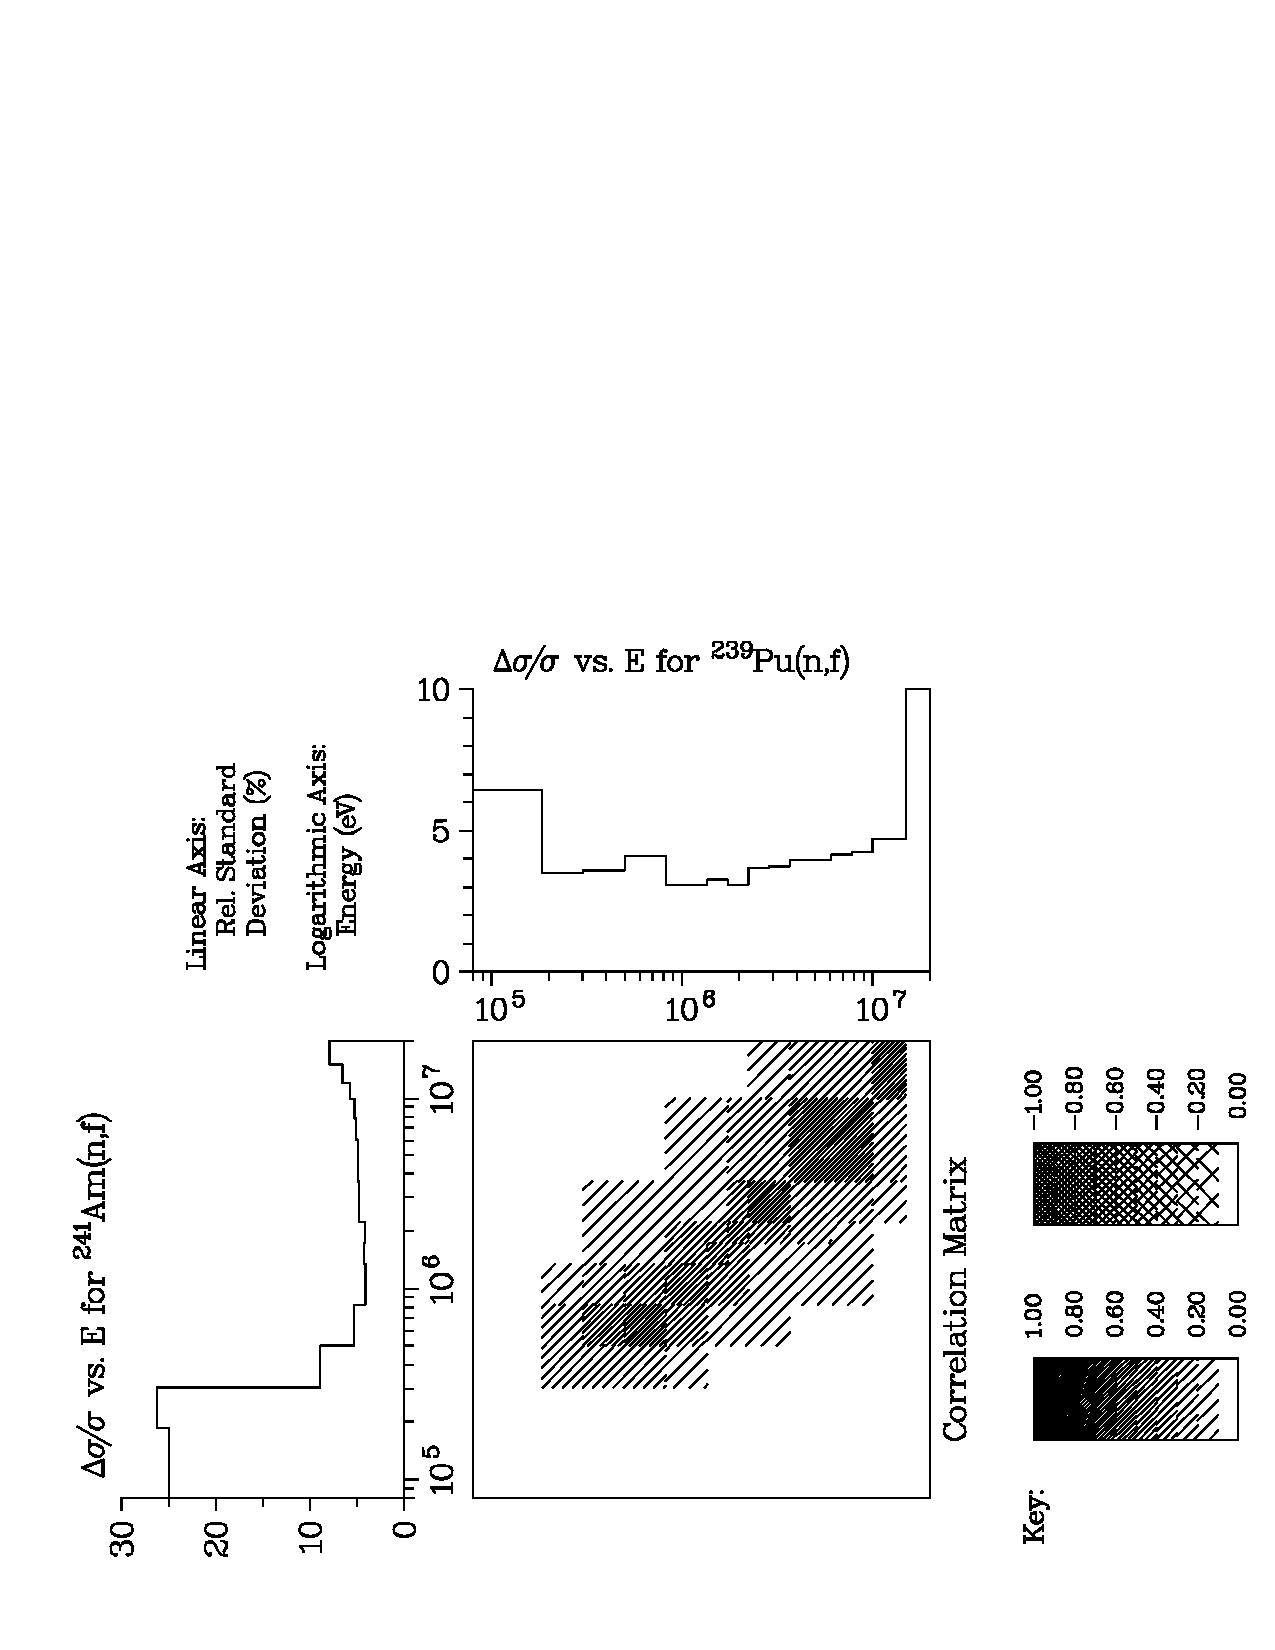
\includegraphics[keepaspectratio, height=5in, angle=270]{figs/errorr2ack}
\caption[Ratioed covariance data for $^{239}$Pu(n,f) and $^{241}$Am(n,f)
 cross sections]{Covariance data for $^{239}$Pu(n,f) with $^{241}$Am(n,f).
 This older figure illustrates the black \& white option for covariance
 plots using hatching to represent levels of correlation.}
\label{ratcov}
\end{figure}

\subsection{Multigroup Processing of Resonance-Parameter Uncertainties}
\label{ssERRORR_MGRR}

In some materials, and in certain energy regions, the cross-section
uncertainty is dominated by the uncertainty in resolved resonance
parameters.  As described above, there are several formats available
in the ENDF-6 format for describing resonance covariances.  When using
the early ENDF-5 format (which is available in the ENDF-6 format as
\cword{LCOMP}=0) the resonance-parameter contribution to the uncertainty
in infinite-dilution fission and capture cross sections is included
automatically when cross-section covariances are processed.  The
contribution is obtained from the Breit-Wigner formulae for the
fission and capture areas of a resonance, $A_f$ and $A_{\gamma}$.
By differentiating these formulae with respect to the resonance
parameters, one obtains a set of sensitivities.  With these
sensitivities and the covariance matrix of the parameters from
MF32, one can apply the propagation-of-errors formula to obtain
the covariances ${\rm cov}(A_{\gamma},A_{\gamma})$,
${\rm cov}(A_{\gamma},A_f)$, and ${\rm cov}(A_f,A_f$).

The resonance contribution is properly weighted with the isotopic
abundance and the ratio of the weight function at the resonance to the
average weight in the group.  It is assumed, however, that the area of
a resonance lies entirely within the group that contains the resonance
energy $E_r$.  Because of this assumption, and because ENDF-5 and the
\cword{LCOMP}=0 option of ENDF-6 provide no correlations between
parameters of different resonances, the calculated resonance-parameter
contribution affects only the diagonal elements of the affected
matrices, ${\rm cov}[X_K(a),X_K(b)]$.

When one of the more advanced options (\cword{LCOMP}=1 or
\cword{LCOMP}=2) is found in MF32, and for Single-Level
Breit-Wigner\index{Single-Level Breit-Wigner!SLBW},
Multi-Level Breit-Wigner\index{Multi-Level Breit-Wigner!MLBW},
or Reich-Moore\index{Reich-Moore!RM} resonance parameters, the
ERRORR code branches to the ERRORJ\index{ERRORJ} logic.  The resonance
cross sections are computed on a special grid and group averaged.  Then
each parameter is changed in turn to generate new cross sections.
Sensitivity parameters are computed from the differences.  These
sensitivity coefficients are then combined with the covariances of
the parameters to obtain covariances on the multigroup cross sections.
The matrices are very large in many cases, and the folding is
time consuming.  There are two formats in use for the parameter
covariances.  One gives each value in a full computer word.  With
many resonances, this can become very bulky.  The other uses a
more compact representation based on the correlations.  Just a few
digits are used for each correlation, thus reducing the size of
the evaluation.  The coding must reconstruct the actual covariance
values before folding them with the sensitivities, so this
economization doesn't help with the time required to fold the
data in the final cross section covariances.

If Reich-Moore-Limited\index{Reich-Moore-Limited!RML} resonances
are found (\cword{LRF}=7, a different branch is taken.  In this case,
it is possible to use analytic formulas to compute the cross section
sensitivities to the parameters.  These formulas are given in detail
in the SAMMY reference\cite{SAMMY}.  These sensitivities are computed
on a special energy grid and group averaged.  They are then folded
with the parameter covariances as described above to obtain the
cross section covariances.


\subsection{Processing of Lumped-Partial Covariances}
\label{ssERRORR_Lump}

The lumped-partial covariance format, allows the evaluator to
specify a group of nuclear reactions and to give the uncertainty only
in the \underline{sum} of the cross sections for that group of
reactions.  One can, for example, replace 30 or 40 discrete-level
inelastic cross sections with 5 or 6 lumped cross sections when
constructing the covariance files.  Because the volume of the
covariance data varies, in general, as the square of the number of
reactions, this lumping can greatly reduce the size of the files.

The first ENDF evaluation to employ the lumped-partial format was
Young's evaluation\cite{Young-2,Young} for $^7$Li (ENDF/B-V, Rev.~2).
All covariance data for this evaluation have been successfully
processed into multigroup form using ERRORR.  The covariances for
\cword{MT854} (a single real level with an excitation energy of
4.63 MeV) with \cword{MT855} (6 lumped pseudo-levels, with excitation
energies ranging from 4.75 MeV to 6.75 MeV) have been plotted in
Fig.~\ref{licov}.  The large negative correlations along the diagonal
result from the fact that, below 10 MeV, these inelastic reactions are
the major contributors to the relatively well-known tritium production
cross section.  An upward variation in one reaction at a given energy
must be accompanied by a downward change in the other reaction.  As shown
in the plot, the magnitude of this negative correlation diminishes at
higher energies, as other reactions begin to contribute significantly to
the tritium-production cross section.  Plots of this type, prepared using
ERRORR and \hyperlink{sCOVRhy}{COVR}, have proved to be
useful tools in the validation of
the covariance files of new evaluations\cite{LaBauve}.

\begin{figure}[thb]\centering
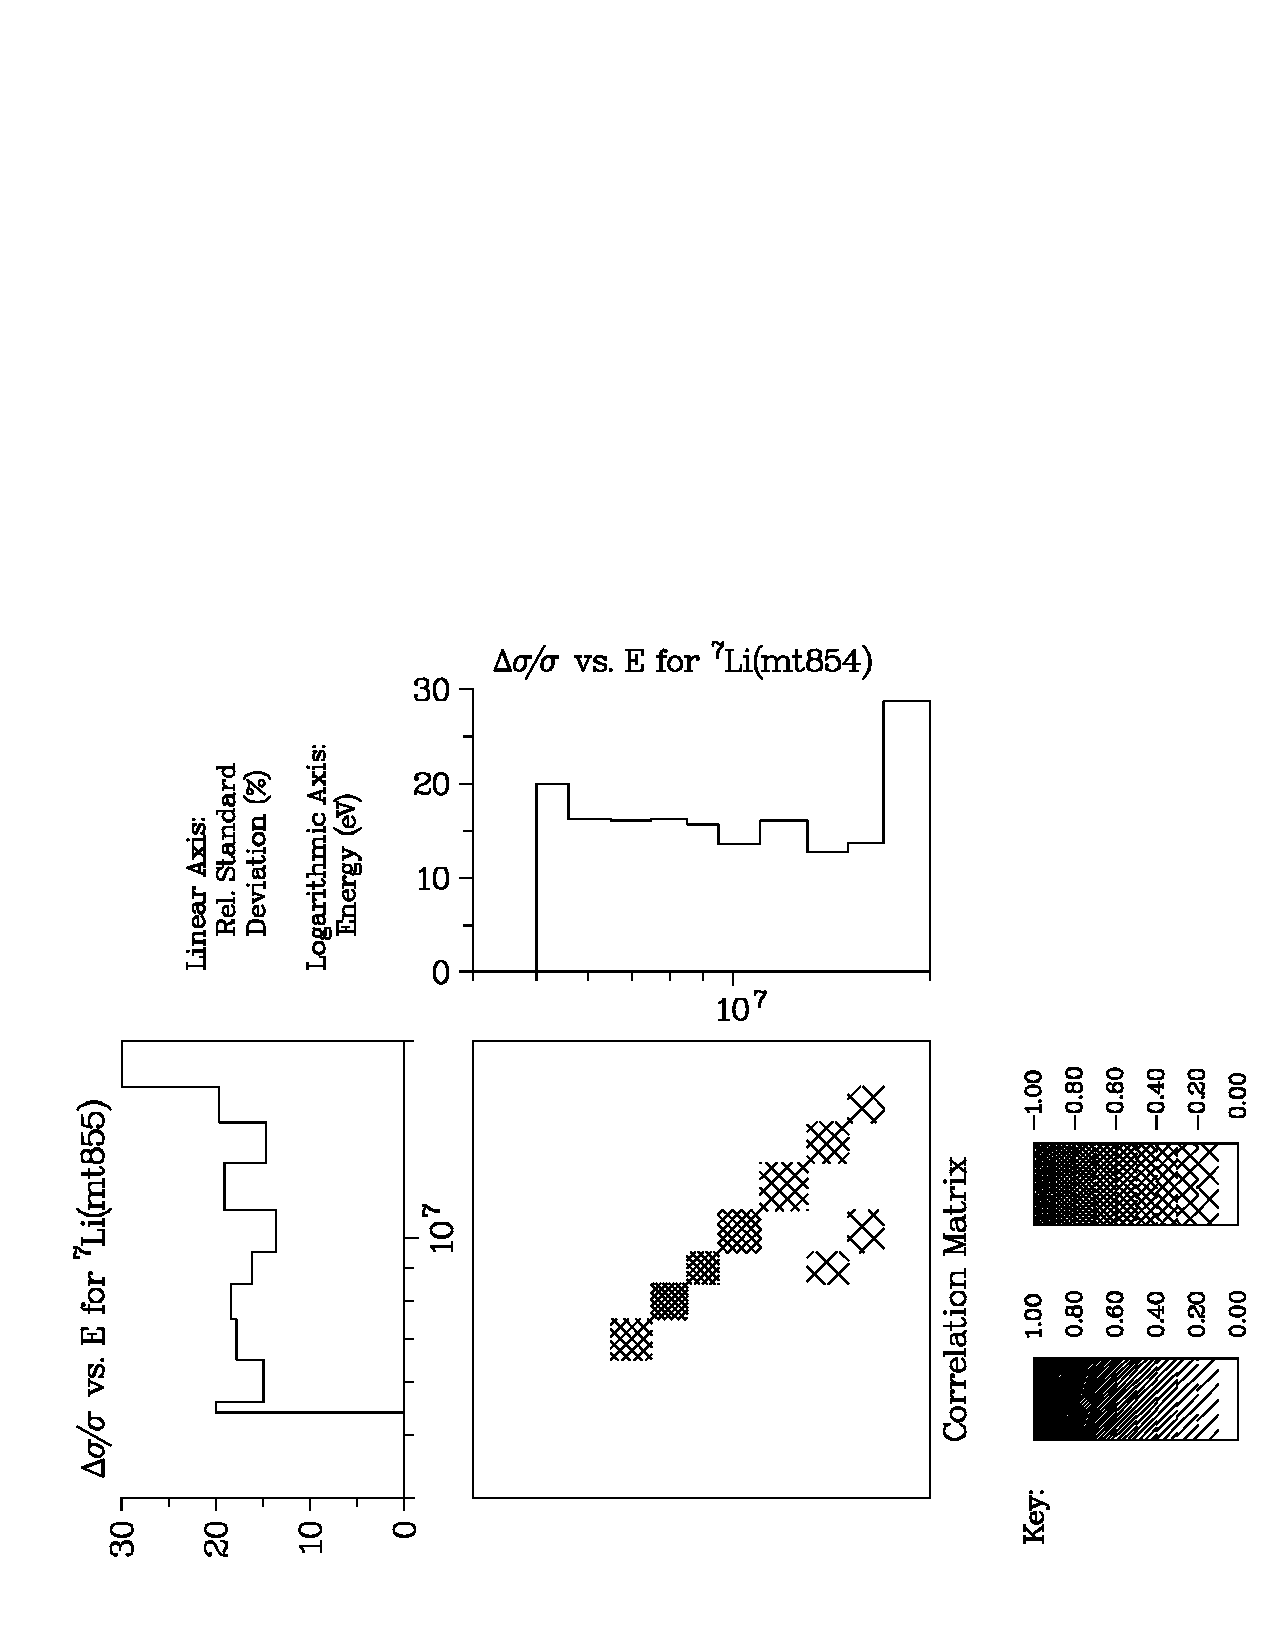
\includegraphics[keepaspectratio, height=5in, angle=270]{figs/errorr3ack}
\caption[$^{7}$Li ``Lumped" covariance data]{Covariance data for $^7$Li
 (MT854) with $^7$Li (MT855).}
\label{licov}
\end{figure}

\subsection{Input Instructions and Sample Input for ERRORR}
\label{ssERRORR_inp}

As an aid to discussions of the user input to ERRORR, we list below the
input instructions that appear as comment cards at the beginning of the
current version of this module.  Since the code and, hence, the
instructions change from time to time, it is always advisable to
consult the comment-card instructions contained in the version of the
code actually being used and not to rely on the instructions published
in any document, including this one.  Note that the word ``tape'' is
used in the instructions to refer to an input or output file,
regardless of the actual storage medium.
\index{ERRORR!ERRORR input}
\index{input!ERRORR}

\newpage
\small
\begin{ccode}

   !--------------------------------------------------------------------
   !
   ! Produce cross section covariances from error files in ENDF format
   !
   ! First, the union energy grid of the users group structure
   ! and the ENDF covariance energies is determined.  The array
   ! of coefficients for derived cross sections is also constructed.
   ! Then multigroup cross sections are computed on the union
   ! grid (see grpav), or they are read from a multigroup cross
   ! section library and then collapsed to the union grid.  The
   ! methods of groupr are used for cross section averaging.  ENDF
   ! covariances and the group cross sections are then combined
   ! to get the basic covariance matrices (see covcal).  Finally,
   ! the basic matrices are combined to get covariances for
   ! derived reactions, the matrices are collapsed to the user's
   ! group structure, and the results are printed and/or written
   ! onto an output gendf tape for later use (see covout).
   !
   ! If resonance parameter covariances are present (MF32), they
   ! are processed and combined with the MF33 covariances.  This
   ! coding was taken from ERRORJ developed in Japan.
   !
   ! Covariances for angular distributions (MF34) and secondary
   ! energy distributions (MF35) can also be processed.
   !
   ! 9/17/2012 ... important changes
   ! - ngout = input gendf input tape
   !           - this tape may contain multiple temperatures,
   !             multiple Legendre moments and multiple sigma-0
   !             data, but ...
   !           - only the first (infinitely dilute) sigma-0
   !             data will be used.
   !
   ! - card 3 is now REQUIRED and the specified temperature must
   !   be one of those on the gendf tape.
   !   - default values are mprint=1, tempin=300
   !
   !---input specifications (free format)---------------------------
   !
   !  card 1
   !    nendf   unit for endf tape
   !    npend   unit for pendf tape
   !    ngout   unit for input group xsec (gendf) tape
   !            (if zero, group xsecs will be calculated)
   !            (if iread eq 2 or if mfcov eq 31, 35 or 40 (see
   !             card 7), then ngout cannot be zero)
   !            (if mfcov eq 35 (see card 7),
   !              ngout cannot be zero)
   !            (default=0)
   !    nout    unit for output covariance tape (default=0)
   !    nin     unit for input covariance tape (default=0)
   !            (nin and nout must be both coded or both binary)
   !    nstan   unit for ratio-to-standard tape (default=0)
   !
   !  card 2
   !    matd    material to be processed
   !    ign     neutron group option
   !            (ign definition same as groupr, except ign=-1,
   !            which means read in an energy grid, as in ign=1,
   !            and supplement this with the endf covariance grid
   !            within the range of the user-specified energies)
   !            (default=1)
   !    iwt     weight function option (default=6)
   !    iprint  print option (0/1=minimum/maximum) (default=1)
   !    irelco  covariance form (0/1=absolute/relative) (default=1)
   !
   !  card 3    (*** REQUIRED for njoy2012 and later ***)
   !    mprint  print option for group averaging (0/1=min (default)/max)
   !    tempin  temperature (default=300)
   !
   !---for endf/b version 4 (iverf=4) only--------------------------
   !
   !  card 4
   !    nek     number of derived xsec energy ranges
   !            (if zero, all xsecs are independent)
   !  card 5    (omit if nek=0)
   !    ek      nek+1 derived xsec energy bounds
   !  card 6    (omit if nek=0)
   !    akxy    derived cross section coefficients, one row/line
   !
   !---for endf/b version 5 or 6 (iverf=5 or 6) only------------------------
   !
   !  card 7
   !    iread   0/1/2=program calculated mts/input mts and eks/
   !            calculated mts plus extra mat1-mt1 pairs from input
   !            (default=0)
   !    mfcov   endf covariance file (31, 33, 34, 35 or 40) to be
   !            processed (default=33).
   !            note--contribution to group cross section
   !            covariances from resonance-parameter uncertainties
   !            (mf=32) is included when mfcov=33 is specified.
   !            (mf=-33) high speed calc for test case
   !            (mf=333) hight speed calc for test case (faster)
   !    irespr  processing for resonance parameter covariances
   !            (mf=32) (default=1)
   !            0 = area sensitivity method
   !            1 = 1\% sensitivity method
   !    legord  legendre order for calculating covariances (default=1)
   !            (if mfcov is not 34, legord is ignored)
   !    ifissp  subsection of the fission spectrum covariance
   !            matrix to process (default=-1 which means process
   !            the subsection that includes efmean).  The value
   !            for ifissp that appears in njoy's standard output
   !            will equal the subsection containing efmean.
   !            (if mfcov is not 35, ifissp is ignored)
   !    efmean  incident neutron energy (eV).  Process the covar-
   !            iance matrix subsection whose energy interval in-
   !            cludes efmean.  if ifissp=-1 and efmean is not
   !            specified, set efmean=2.e6_kr.  But if there is only
   !            one subsection, process it and if the input efmean
   !            was not within this subsection's energy range then
   !            redefine efmean to equal the average energy for
   !            this subsection.
   !            (if mfcov is not 35, efmean is ignored)
   !    dap     user specified scattering radius uncertainty, given
   !            as a fraction (i.e., dap=0.1 means 10\% uncertainty
   !            in the scattering radius).  The default value is
   !            zero.  This variable is only defined for mfcov=33
   !            and if non-zero will be used in lieu of any data
   !            that might have been read from the nendf tape.
   !
   !  following cards only if iread eq 1
   !  card 8
   !    nmt     no. mts to be processed
   !    nek     no. derived cross section energy ranges
   !            (if zero, all xsecs are independent)
   !  card 8a
   !    mts     nmt mts
   !  card 8b   (omit if nek=0)
   !    ek      nek+1 derived cross section energy bounds
   !  card 9    (omit if nek=0)
   !    akxy    derived cross section coefficients, one row/line
   !
   !  following card only if iread eq 2
   !  card 10
   !    mat1    cross-material reaction to be added to
   !    mt1         covariance reaction list.
   !            repeat for all mat1-mt1 pairs desired
   !            terminate with mat1=0.
   !
   !  following card only if nstan ne 0
   !  card 11
   !    matb    standards reaction referenced
   !    mtb         in matd.
   !    matc    standards reaction to be
   !    mtc         used instead.
   !            repeat for all standard reactions to be redefined.
   !            terminate with matb=0.
   !  note.  if matb(1) and mtb(1) are negative, then matc(1) and
   !    mtc(1) identify a third reaction, correlated with matd thru
   !    the use of the same standard.  covariances of all reactions
   !    in matd (which reference the standard) with the reaction
   !    matc(1)-mtc(1) will be produced.  the standard reaction
   !    must be identified on card 10 and repeated as the negative
   !    entries on card 11.  the group xsec tape ngout must include
   !    all covariance reactions in matd, plus matc(1)-mtc(1).
   !
   !  card 12a (for ign eq 1 or ign eq -1)
   !    ngn     number of groups
   !  card 12b
   !    egn     ngn+1 group bounds (ev)
   !  card 13 (for iwt eq 1 only)
   !    wght    weight function as a tab1 record
   !  card 13b  analytic flux parameters (iwt=4 only)
   !    eb      thermal break (ev)
   !    tb      thermal temperature (ev)
   !    ec      fission break (ev)
   !    tc      fission temperature (ev)
   !
   ! ---options for input variables------------------------------------
   !
   !      ign          meaning
   !      ---          -------
   !       1           arbitrary structure (read in)
   !      -1           arbitrary structure (read in), supplemented with endf
   !                   covariance grid
   !       2           csewg 239-group structure
   !       3           lanl 30-group structure
   !       4           anl 27-group structure
   !       5           rrd 50-group structure
   !       6           gam-i 68-group structure
   !       7           gam-ii 100-group structure
   !       8           laser-thermos 35-group structure
   !       9           epri-cpm 69-group structure
   !      10           lanl 187-group structure
   !      11           lanl 70-group structure
   !      12           sand-ii 620-group structure
   !      13           lanl 80-group structure
   !      14           eurlib 100-group structure
   !      15           sand-iia 640-group structure
   !      16           vitamin-e 174-group structure
   !      17           vitamin-j 175-group structure
   !      18           xmas nea-lanl
   !      19           ecco  33-group structure
   !      20           ecco 1968-group structure
   !      21           tripoli 315-group structure
   !      22           xmas lwpc 172-group structure
   !      23           vit-j lwpc 175-group structure
   !      24           shem cea 281-group structure
   !      25           shem epm 295-group structure
   !      26           shem cea/epm 361-group structure
   !      27           shem epm 315-group structure
   !      28           rahab aecl 89-group structure
   !      29           ccfe   660-group structure  (30 MeV)
   !      30           ukaea 1025-group structure  (30 MeV)
   !      31           ukaea 1067-group structure (200 MeV)
   !      32           ukaea 1102-group structure   (1 GeV)
   !      33           ukaea  142-group structure (200 MeV)
   !      34           lanl 618-group structure
   !
   !      iwt          meaning
   !      ---          -------
   !       1           read in smooth weight function
   !       2           constant
   !       3           1/e
   !       4           1/e + fission spectrum + thermal maxwellian
   !       5           epri-cell lwr
   !       6           (thermal) -- (1/e) -- (fission + fusion)
   !       7           same with t-dep thermal part
   !       8           thermal--1/e--fast reactor--fission + fusion
   !       9           claw weight function
   !      10           claw with t-dependent thermal part
   !      11           vitamin-e weight function (ornl-5505)
   !      12           vit-e with t-dep thermal part
   !
   !--------------------------------------------------------------------

\end{ccode}
\normalsize

As an example of the use of these commands, here is the input used
to produce Fig.~\ref{b10cov}, the covariance plot for $^{10}$B
from ENDF/B-VII.0.

\small
\begin{ccode}

    1. errorr
    2. 31 32 0 33/
    3. 525 3 9 1 1/
    4. 0 0./
    5. 0 33/
    6. covr
    7. 33 0 34/
    8. 1/
    9. /
   10. /
   11. 525/
   12. viewr
   13. 34 35/
   14. stop

\end{ccode}
\normalsize

\noindent
The line numbers are for reference and are not part of the input.
Identical versions of the ENDF/B-VII.0 file for $^{10}$B can be
copied to \cword{tape31} and \cword{tape32}.  The ERRORR output
will appear on \cword{tape33}.  In this sample input deck, that file
is the input file to \hyperlink{sCOVRhy}{COVR} which
generates the plot instructions that are subsequently written to
\cword{tape34}.  Line 3 defines the material to be
processed (525, or $^{10}$B), the group structure, the weight function,
the listing option, and requests relative covariances.  Line 4 turns
off printing for the group averaging and requests zero temperature.
Users are cautioned that line 4 is now required in all ERRORR input decks
whereas in njoy99 it is only required when ngout is zero.  Line 5
asks the program to calculate the MT numbers to be processed
and to work with File 33.  The \hyperlink{sCOVRhy}{COVR} and
\hyperlink{sVIEWRhy}{VIEWR} input in lines 6 through
13 act to prepare the graph as seen in Fig.~\ref{b10cov}.

The follwing paragraphs give more detail on how the various
input parameters are used.

\cword{npend, ngout } \ldots\hspace{.1in}The user must supply either a
PENDF\index{PENDF} tape on unit \cword{npend} or a GENDF\index{GENDF}
tape on unit \cword{ngout}.  If present, the \cword{npend} tape should
contain pointwise (resonance-reconstructed, but not multigrouped) data
and is normally produced with the
\hyperlink{sRECONRhy}{RECONR}\index{RECONR} module.  If the
resonance region is of no interest, a simple copy of the ENDF tape will
suffice for this purpose.  The GENDF tape, if present, should contain
multigroup cross sections and/or $\overline{\nu}$ values, produced by
the \hyperlink{sGROUPRhy}{GROUPR}\index{GROUPR} module,
for all reactions for which multigroup
covariances are needed.  Group cross sections need not be in the same group
structure as the requested output covariances, although if the input
group structure is much coarser than the output structure, rather crude
approximations will be made in deriving an effective set of fine-group
cross sections and fluxes from the coarse input data.  Certain types
of covariance calculations related to fission data or the computation
of cross-material covariances require the user to supply a GENDF
tape on \cword{ngout} (that is, \cword{npend} must be zero).

\cword{nin, nout } \ldots\hspace{.1in}Input and output covariance
tapes in the user's group structure may either be both formatted or
both binary.  Although ERRORR lacks an explicit multimaterial
loop, the same effect can be achieved by executing a series of ERRORR
runs, with the output of one run becoming the input of the next.  Only
two unit numbers need be employed, with the data going back and forth
between them until the multimaterial library is complete.  To save
time, binary files should be used for this
purpose.  \hyperlink{sMODERhy}{MODER}\index{MODER}
can be used to convert the final output tape from binary to formatted
form, if desired.

\cword{nstan } \ldots\hspace{.1in}This tape is needed if covariances
are requested for a reaction pair that is related by ratio
measurements, as discussed in Section~\ref{ssERRORR_Ratio}.  The ENDF
subsection for
such a pair will contain an NC-type sub-subsection with
\cword{LTY}=1, 2, or 3.  The specific pairs in ENDF/B-V that require
a standards tape are tabulated  in Table~\ref{ratios}
(Section~\ref{ssERRORR_Ratio}).
For other evaluations, one can assume \cword{nstan} is not needed.
The code will stop with a clear error message if this assumption
proves incorrect.

\cword{iread } \ldots\hspace{.1in}For ENDF/B versions 5 and 6, the list of
reactions for which covariances are produced is constructed in one of
several ways, depending on the value of \cword{iread}.  If
\cword{iread}=0, which is the generally recommended choice,
the reaction list is assumed to be identical to the list of sections
contained in the ENDF/B covariance file (see \cword{mfcov} below).
Although \cword{iread}=0 is the most convenient option for constructing
the list of covariance reactions, it leads to a problem if some
covariance reactions have thresholds above the highest group boundary
of the user's structure.  These reactions will have zero cross sections
in all groups and thus will be omitted from \cword{ngout}.  To avoid
this difficulty, ERRORR automatically resets the user's highest group
boundary to 20 MeV whenever \cword{iread}=0.  By judicious choice of
weighting functions, one can minimize the effect of this resetting on
the other cross sections and their covariances.

If \cword{iread}=1, only the covariance reactions specifically
named by the user will be included in the reaction list.  For certain
applications, this option can save considerable execution time.
However, to take advantage of this option, the user must examine the
ENDF evaluation visually to determine which reactions are derived
from other reactions in each energy region.  As discussed in
Section~\ref{ssERRORR_Str}, this information is contained in NC-type
sub-subsections
with \cword{LTY}=0.  Incorrect results will be obtained if one requests
processing for a given reaction without processing all of the reactions
from which the given reaction is derived in the energy region spanned
by the output group structure.  The inclusion of those reactions may
require, in turn, additional inclusions as well.  In addition, the user
must extract from the file (and enter into the input) the appropriate
derivation coefficients and the energy ranges over which they
apply.  An example of the required input is presented below in the
discussion of the parameters \cword{nmt}, \cword{nek}, \cword{mts},
\cword{ek}, and \cword{akxy}.

If \cword{iread}=0 or 1, a complete set of covariance matrices
is written.  That is, covariance matrices are produced for
every reaction-pair combination that can be formed from the
given reaction list.  For those reaction pairs where the evaluator has
not specified the covariances, the output matrix contains only zeros.

In the evaluation containing cross-material covariances, subsections
involving the other materials will be ignored if \cword{iread}=0 or
1.  These subsections can be selectively processed by
specifying \cword{iread}=2.  If \cword{iread}=2, the reaction list is
initially constructed in the same way as for \cword{iread}=0.  This
list is then supplemented with a list of extra reactions (MAT1$_k$,
MT1$_k$) (where (MAT1$_k$ $\neq$ MATD), specified by the user.  The
output in this case contains matrices for all of the (MATD, MT$_i$;
MATD,,MT$_j$) combinations, as before, plus matrices for all
(MATD, MT$_i$; MAT1$_k$, MT1$_k$) combinations.  However, covariances
among the extra reactions, for example (MAT1$_k$, MT1$_k$;
MAT1$_m$,,MT1$_m$), are not computed.  Input for an example problem that
illustrates the use of \cword{iread}=2 is given below, in the
discussion of \cword{mfcov}.  That discussion also includes an
illustration of the set of MAT/MT combinations that
are processed when \cword{iread}=2.

\cword{mfcov} \ldots\hspace{.1in} is used to specify whether
covariances of $\overline{\nu}$ (\cword{mfcov}=31), cross
sections (\cword{mfcov}=33), angular distributions (\cword{mfcov}=34),
secondary energy distributions (\cword{mfcov}=35), or radioactive nuclide
production (\cword{mfcov}=40) are needed.  If \cword{mfcov}=31, 35, or 40,
it is necessary to supply multigrouped
cross sections and $\overline{\nu}$ values on a GENDF tape
that is, \cword{npend} must be 0); the sample problem below shows
the calculational sequence required.  The parameter \cword{mfcov}=32
is reserved for a planned future capability to compute
uncertainties in self-shielded cross sections.  If \cword{mfcov=33},
the contribution of the uncertainty in individual resonance parameters
(File 32) is included in the calculated uncertainty in
infinite-dilution group cross sections.  Given below is the complete
NJOY input for a calculation of a multigroup $\overline{\nu}$
covariance library for $^{238}$U, including five cross-material
reactions.

\small
\begin{ccode}

   moder / mount ENDF tapes 515, 516, and 555 on units 20, 21, and 22.
   1 -23/
   'ENDF/B-V NUBAR COVARIANCE MATERIALS'/
   20 1380/
   20 1381/
   21 1390/
   22 1395/
   22 1398/
   20 1399/
   0/
   moder / copy ENDF for use as a PENDF.
   -23 -24/
   groupr / prepare GENDF with multigrouped nubars.
   -23 -24 0 25/
   1380 3 0 3 0 1 1 0/
   'BIG3 + 2 NUBAR'/
   0./
   1.e10/
   3 452 'TOTAL NUBAR'/
   0/
   1381/
   3 452 'TOTAL NUBAR'/
   0/
   1390/
   3 452 'TOTAL NUBAR'/
   0/
   1395/
   3 452 'TOTAL NUBAR'/
   0/
   1398/
   3 452 'TOTAL NUBAR'/
   3 455 'DELAYED NUBAR'/
   3 456 'PROMPT NUBAR'/
   0/
   1399/
   3 452 'TOTAL NUBAR'/
   0/
   0/
   errorr / prepare multigroup nubar covariance library.
   -23 0 25 26/
   1398 -1 1 1/
   0 0. /
   2 31/
   1380 452/
   1381 452/
   1390 452/
   1395 452/
   1399 452/
   0/
   1/
   1.e7 1.7e7/
   stop

\end{ccode}
\normalsize

Note the use of the \hyperlink{sMODERhy}{MODER} module
to prepare a special ENDF tape
containing selected evaluations from other ENDF tapes.  Because only
high-energy $\overline{\nu}$ data are requested (10 -- 17 MeV), it is
unnecessary to use \hyperlink{sRECONRhy}{RECONR} to prepare
a PENDF tape for \hyperlink{sGROUPRhy}{GROUPR}.  A copy
of the ENDF tape is used instead.

Following the prescription given in the discussion of the
\cword{iread}=2 option, with this particular input, covariance matrices
will be produced for those reaction pairs marked with an X in
Table~\ref{pairs}.  The remaining non-redundant possibilities (dashes)
can be filled in with successive ERRORR runs with
\cword{MATD}=1380, 1381, etc.

\begin{table}[t]
\caption{Reaction pairs in the ENDF/B-V $^{238}$U evaluation}
\label{pairs}
\begin{center}
\begin{tabular}{|l|c|c|c|c|c|c|c|c|c|}
\hline
    & a  &  b  &  c  &  d  &  e  &  f  &  g  &  h  & i \\ \cline{1-10}
a = (1398,452) &  X  &  X  &  X  &  X  &  X  &  X  &  X  &  X  &  X \\
b = (1398,455) &  &  X  &  X &  X  &  X  &  X  &  X  &  X  &  X \\
c = (1398,456) &  &  &  X &  X  &  X  &  X  &  X  &  X  &  X  \\
d = (1380,452) &  &  &  &  -- &  -- &  --  &  -- &  -- &  -- \\
e = (1381,452) &  &  &  &     &  -- &--  &  -- &  -- &  -- \\
f = (1390,452) &  &  &  &     &     &  --  &  -- &  -- &  -- \\
g = (1395,452) &  &  &  &     &     &      &  -- &  -- &  --  \\
h = (1398,452) &  &  &  &     &     &      &     &  -- &  --  \\
i = (1399,452) &  &  &  &     &     &      &     &     &  -- \\
\cline{1-10}
\end{tabular}
\end{center}
\end{table}

\cword{nwt}, \cword{nek}, \cword{mts}, \cword{ek}, \cword{akxy}
\ldots\hspace{.1in}
For ENDF/B version 5, if \cword{iread}=1, the user specifies a subset of the
evaluator's covariance reactions (that is, a subset of the sections
of \cword{mfcov}), as the particular set of reactions for which
processing is requested.  These \cword{nmt} desired reactions are
entered in the array \cword{mts}.  As mentioned in the discussion of
\cword{iread} above, one must also include in the \cword{mts} array all
reactions from which the desired reactions are derived.

Another requirement of the \cword{iread}=1 option is that the actual
derivation coefficients, called \cword{akxy} in the code, but called
$C_I(a,c)$ in the discussion in Section~\ref{ssERRORR_summ}, must be
entered in the
ERRORR input for \cword{nek} energy ranges spanning the output group
structure.  Adjacent ENDF derivation ranges may be merged into a
single range if the derivation-coefficient matrix for the \cword{nmt}
explicitly requested reactions is the same in each of the adjacent
ranges.  The ordering of the $C_I(a,c)$ data is as follows: on one line
of input the coefficients are specified for a fixed $a$-value and for
all $c$-values ranging from 1 to \cword{nmt}.  One such line is given
for each $a$-value.  Finally, there is an outer loop over the
\cword{nek} energy ranges.  An example of the input that is required
for \cword{iread}=1 is given below for the case of ENDF/B-V carbon
\cword{MAT}=1306.  It will be necessary to examine File 33 of the
evaluation (which is available on the ENDF/B-V standards file, Tape
511), in order to understand the details of this example.

\small
\begin{ccode}

   moder
   20- 21/
   moder / copy ENDF for use as a PENDF.
   -21 -22/
   errorr
   -21 -22 0 -23/
   1306 3 1/
   2 0 0/
   1 33/
   7 3/
   1 2 4 102 103 104 107/
   1.e-5 2e6 4.812e6 2e7/
   0 1 0 1 0 0 0/
   0 1 0 0 0 0 0/
   0 0 1 0 0 0 0/
   0 0 0 1 0 0 0/
   0 0 0 0 1 0 0/
   0 0 0 0 0 1 0/
   0 0 0 0 0 0 1/
   1 0 0 0 0 0 0/
   0 1 0 0 0 0 0/
   0 0 1 0 0 0 0/
   0 0 0 1 0 0 0/
   0 0 0 0 1 0 0/
   0 0 0 0 0 1 0/
   0 0 0 0 0 0 1/
   1 0 0 0 0 0 0/
   0 1 0 0 0 0 0/
   1 -1 0 -1 -1 -1 -1/
   0 0 0 1 0 0 0/
   0 0 0 0 1 0 0/
   0 0 0 0 0 1 0/
   0 0 0 0 0 0 1/
   stop

\end{ccode}
\normalsize

Note that here, even if the user wanted to process only M=2 and
MT=4, for example, it is nevertheless necessary to include
MT=1, MT=102, MT=103, MT=104, and MT=107, because the \cword{ign}=3
group structure extends to 17.0 MeV, and above 4.812 MeV, MT=4 is
derived from the relation
\begin{equation}
\sigma_4 = \sigma_1 - \sigma_2 - \sigma_{102} - \sigma_{103} -
\sigma_{104} - \sigma_{107} \; .
\end{equation}
See the corresponding $C_I(a,c)$ matrix in the input above (the
last 7 lines before \cword{stop}).

\cword{matb}, \cword{mtb}, \cword{matc}, \cword{mtc} \ldots\hspace{.1in}Card 11
provides a capability to remap all references to a given standards reaction
\cword{(matb, mtb)} appearing in NC-type sub-subsections with
\cword{lty}=1, 2, or 3 into references to a different
reaction \cword{(matc, mtc)}.  (See the discussion of ratio measurements
in Section~\ref{ssERRORR_Ratio}.)  This facility is useful if the evaluation
\cword{(matb, mtb)} is for some reason unavailable.  Up to 5 such
standards can be redefined.  As explained in the note on the input
instructions at the beginning of this section, Card 11 is also used, if
\cword{matb(1)} and \cword{mtb(1)} are negative, to process covariances
between two distinct reactions, both measured relative to a common
standards reaction.  This was referred to as the \cword{lty}=4 case
in Section~\ref{ssERRORR_Ratio}.  A separate ERRORR run is required for
each requested \cword{lty}=4 reaction pair.

This second use of Card 11 is illustrated in the sample NJOY input
listed below, which is the input used to generate and plot the
data shown in Fig.~\ref{ratcov}.  The input to the
\hyperlink{sCOVRhy}{COVR}\index{COVR}
module contained in the sample is explained in the following chapter.

\small
\begin{ccode}

   mount T562 on tape30
   mount T563 on tape40
   mount T560 on tape50

   moder
   1 -31/
   'U235 FROM T562'/
   30 1395/
   0/
   moder
   1 -21/
   'AM241 FROM T560 AND PU239 FROM T563'/
   50 1361/ AM241
   40 1399/ PU239
   0/
   reconr
   -21 -22/
   '10 PERCENT PENDF FOR AM241 AND PU239'/
   1361/
   .1/
   1399/
   .1/
   0/
   GROUPR
   -21 -22 0 -24/
   1361 3 0 2 0 1 1 0/
   '30 GROUP XSECS FOR AM241 AND PU239'/
   0/
   1e10/
   3 1/
   3 2/
   3 4/
   3 16/
   3 17/
   3 18/
   3 102/
   0/
   1399
   3 18/
   3 102/
   0/
   0/
   errorr
   -21 0 -24 -25 0 -31/
   1361 3 1 1/
   0 0. /
   0 33/
   0/
   errorr
   -21 0 -24 -28 -25 -31/
   1399 3 1 1/
   0 0. /
   2 33/
   1395 18/
   0/
   -1395 -18 1361 18/
   0/
   covr
   -28/
   0 0 0 8e4/
   1 1 0 0 2/
   1399 18 1361 18/
   stop

\end{ccode}
\normalsize

The input for a File 34 case preparing covariances for an angular
distribution is shown below.  This is the input that produced
Fig.~\ref{mf34cov} shown above.  This deck runs a job sequence
that includes \hyperlink{sMODERhy}{MODER} (ASCII-to-binary
conversion), \hyperlink{sRECONRhy}{RECONR} and
\hyperlink{sBROADRhy}{BROADR} (cross section reconstruction
to 300K), \hyperlink{sGROUPRhy}{GROUPR}
(unweighted, infinitely dilute multigroup cross sections plus
average $\bar{\mu}$), ERRORR (specifying \cword{mfcov}=34 for
$\bar{\mu}$ covariance processing), and
\hyperlink{sCOVRhy}{COVR} and \hyperlink{sVIEWRhy}{VIEWR} (for plot
generation and conversion to Postscript format).  The input on
\cword{tape20} was the JENDL-3.3 evaluation for $^{238}$U.

\small
\begin{ccode}

   moder
    20 -21 /
   reconr
    -21 -22 /
    'processing jendl-3.3 u-238.'/
    9237 0 0 /
    0.001 /
    0 /
   broadr
    -21 -22 -23 /
    9237 1 0 0 0 /
    0.001 /
    300. /
    0 /
   groupr
    -21 -23 0 91 /
    9237 3 0 2 1 1 1 0 /
    'test'/
    300. /
    1.0e10 /
    3 /
    3 251 'mubar' /
    0 /
    0 /
   --
   -- process mf34
   errorr
    -21 0 91 27 0 0 /
    9237 3 2 1 1 /
    0 300. /
    0 34 1 1 -1 /
   --
   -- make mf34 plot file.
   covr
    27 0 37 /
    1 /
    /
    /
    9237 /
   --
   -- make mf34 postscript file.
   viewr
    37 47 /
   stop

\end{ccode}
\normalsize

The input for the File 35 case that produced the plot of secondary
energy covariances seen in Fig.~\ref{mf35cov} is given below.
This is a problem taken from the NJOY test suite that uses a
fictitious input file for $^{252}$Cf.  The
\hyperlink{sGROUPRhy}{GROUPR} and ERRORR
inputs specify a user-defined group structure that corresponds to
the energies listed in File 1 of the evaluation with the
uncertainties provided by the evaluator.  This makes it easy
to verify that the results agree with the evaluator's intent.

\small
\begin{ccode}

   --
   -- Copy ascii input to binary.
   moder
    20 -21 /
   --
   -- Resonance reconstruction, to 0.1\%.
   reconr
    -21 -22 /
    'processing e70 252Cf with decay mf5/mt18 & mf35/mt18'/
    9999 0 0 /
    0.001 /
    0 /
   --
   -- Doppler broaden to 300K.
   broadr
    -21 -22 -23 /
    9999 1 0 0 0 /
    0.001 /
    300. /
    0 /
   --
   -- Group average, 300K with mf35 group structure.
   --  - All file 3 cross sections plus fission spectrum.
   groupr
    -21 -23 0 91 /
    9999 1 0 2 1 1 1 1 /
    'test'/
    300. /
    1.0e10 /
    71 / # of groups, energy boundaries follow:
    1.000000-5 1.500000+4 3.500000+4 5.500000+4 7.500000+4
    9.500000+4 1.150000+5 1.350000+5 1.650000+5 1.950000+5
    2.250000+5 2.550000+5 3.050000+5 3.550000+5 4.050000+5
    4.550000+5 5.050000+5 5.550000+5 6.050000+5 6.550000+5
    7.050000+5 7.550000+5 8.050000+5 8.550000+5 9.050000+5
    9.550000+5 1.050000+6 1.150000+6 1.250000+6 1.350000+6
    1.450000+6 1.550000+6 1.650000+6 1.750000+6 1.850000+6
    1.950000+6 2.150000+6 2.350000+6 2.550000+6 2.750000+6
    2.950000+6 3.250000+6 3.550000+6 3.850000+6 4.150000+6
    4.450000+6 4.750000+6 5.050000+6 5.550000+6 6.050000+6
    6.550000+6 7.050000+6 7.550000+6 8.050000+6 8.550000+6
    9.050000+6 9.550000+6 1.005000+7 1.055000+7 1.105000+7
    1.155000+7 1.205000+7 1.255000+7 1.305000+7 1.355000+7
    1.405000+7 1.460000+7 1.590000+7 1.690000+7 1.790000+7
    1.910000+7 2.000000+7/
    3 /
    5 18  'chi' /
    0 /
    0 /
   --
   -- ERRORJ, mf35
   errorr
    20 0 91 28 0 0 /
    9999 1 2 1 1 /
    0 300. /
    0 35 1 1 -1 1.23e6 /
    71 / # of groups, energy boundaries follow:
    1.000000-5 1.500000+4 3.500000+4 5.500000+4 7.500000+4
    9.500000+4 1.150000+5 1.350000+5 1.650000+5 1.950000+5
    2.250000+5 2.550000+5 3.050000+5 3.550000+5 4.050000+5
    4.550000+5 5.050000+5 5.550000+5 6.050000+5 6.550000+5
    7.050000+5 7.550000+5 8.050000+5 8.550000+5 9.050000+5
    9.550000+5 1.050000+6 1.150000+6 1.250000+6 1.350000+6
    1.450000+6 1.550000+6 1.650000+6 1.750000+6 1.850000+6
    1.950000+6 2.150000+6 2.350000+6 2.550000+6 2.750000+6
    2.950000+6 3.250000+6 3.550000+6 3.850000+6 4.150000+6
    4.450000+6 4.750000+6 5.050000+6 5.550000+6 6.050000+6
    6.550000+6 7.050000+6 7.550000+6 8.050000+6 8.550000+6
    9.050000+6 9.550000+6 1.005000+7 1.055000+7 1.105000+7
    1.155000+7 1.205000+7 1.255000+7 1.305000+7 1.355000+7
    1.405000+7 1.460000+7 1.590000+7 1.690000+7 1.790000+7
    1.910000+7 2.000000+7/
   --
   -- make plot file.
   covr
    28 0 38 /
    1 /
    1.e3 /
    /
    9999 /
   --
   -- make postscript file.
   viewr
    38 39 /
   stop
\end{ccode}
\normalsize

The final example gives the input used to prepare Fig.~\ref{mf40cov}
showing the uncertainties in radionuclide production for $^{93}$Nb.
This is a fairly elaborate input deck, as it includes
\hyperlink{sGROUPRhy}{GROUPR}/ERRORR/
\hyperlink{sCOVRhy}{COVR}/\hyperlink{sVIEWRhy}{VIEWR}
processing for both File 3 and File 10.

\small
\begin{ccode}

   -- Extract/convert neutron evaluated data
   moder
    1 -21/
    '41-Nb-93 from e70'/
    20 4125/
    0/
   --
   -- Make an ASCII copy
   moder
    -21 41 /
   --
   -- Reconstruct xs
   reconr
    41 42/
    'pendf for 41-Nb-93'/
    4125 2/
    0.001 0. 0.003/
    '41-Nb-93 from e70'/
    'Processed with NJOY'/
    0/
   --
   -- Doppler broaden xs
   broadr
    41 42 43/
    4125 1 0 0 0./
    0.001 2.0e6 0.003/
    300./
    0/
   --
   -- groupr, process all file 3 reactions:
   groupr
    41 43 0 44 /
    4125 1 0 6 0 1 1 1 /
    '41-Nb-93 from e70 with NJOY'/
    300. /
    1.e10 /
    21 /
    1.e-5 0.625 10.7 100.0 1.e3 1.e4 1.e5 1.e6
    2.e6 3.e6 4.e6 5.e6 6.e6 7.e6 8.e6 9.e6 10.e6
    12.e6 14.e6 16.e6 18.e6 20.e6 /
    3 /
    0/
    0/
   --
   -- errorj, process all file 3 reaction uncertainties:
   errorr
    41 43 44 45/
    4125 1 6 1 1 /
    0 300. /
    0 33 /
    21 /
    1.e-5 0.625 10.7 100.0 1.e3 1.e4 1.e5 1.e6
    2.e6 3.e6 4.e6 5.e6 6.e6 7.e6 8.e6 9.e6 10.e6
    12.e6 14.e6 16.e6 18.e6 20.e6 /
   --
   -- create plot of mf33 uncertainty data
   covr
    45 0 55 /
    1 /
    1.e-1 /
    /
    4125 /
   viewr
    55 65 /
   --
   -- groupr, process all file 10 reactions:
   groupr
    41 43 0 46 /
    4125 1 0 6 0 1 1 1 /
    '41-Nb-93 from e70 with NJOY'/
    300. /
    1.e10 /
    21 /
    1.e-5 0.625 10.7 100.0 1.e3 1.e4 1.e5 1.e6
    2.e6 3.e6 4.e6 5.e6 6.e6 7.e6 8.e6 9.e6 10.e6
    12.e6 14.e6 16.e6 18.e6 20.e6 /
    10 /
    0/
    0/
   --
   -- errorj, process all file 10 reaction uncertainties:
   errorr
    41 43 46 47/
    4125 1 6 1 1 /
    0 300. /
    0 40 /
    21 /
    1.e-5 0.625 10.7 100.0 1.e3 1.e4 1.e5 1.e6
    2.e6 3.e6 4.e6 5.e6 6.e6 7.e6 8.e6 9.e6 10.e6
    12.e6 14.e6 16.e6 18.e6 20.e6 /
   --
   -- create plot of mf40 uncertainty data
   covr
    47 0 57 /
    1 /
    1.e3 /
    /
    4125 /
   viewr
    57 67 /
   stop

\end{ccode}
\normalsize

\subsection{ERRORR Output File Specification}
\label{ssERRORR_Out}

The results from ERRORR are written to an output file on unit
\cword{nout}, provided that the input parameter \cword{nout} is
nonzero.  This file contains the user's group structure, the
multigroup cross sections, and either absolute (\cword{irelco}=0) or
relative (\cword{irelco}=1) covariances.  If \cword{nout} is positive,
then a formatted (card-image) file is written, and, if negative, a
binary file is written.  In either case, the output is written with the
standard \hyperlink{sNJOYhy}{NJOY} I/O utilities, and the result
has an ENDF-like structure.  As is the case for ENDF, PENDF, and
GENDF files, ERRORR output files can be converted from binary to
formatted form (and {\it vice versa}) by using the
\hyperlink{sMODERhy}{MODER} module.  The energy-group ordering of
the data written to \cword{nout} follows the ENDF convention, that is,
low-energy groups precede high-energy groups.

It is occasionally of interest to examine a formatted ERRORR output
file visually.  For this and other reasons, we describe below the
detailed form of the formatted output file.  To assist in the
description, we give below an example listing of such a file, which
was produced during the processing of COVFILS-2\cite{COVFILS2}.

The data in the listing are written in the form of standard, 80-column
card-images consisting of 10 data fields.  As in ENDF, the first 6
fields are 11 characters wide and are used for either floating-point
numbers or integers.  The seventh, eighth, ninth, and tenth fields are
4, 2, 3, and 5 characters wide, respectively, and are used for integers
only. The four digits in Field 7 are the \cword{MAT}, or material
number, of the isotope or element; the two digits in Field 8 are the
\cword{MF}, or file number, which indicates the general type of data
(for example, cross-section data {\it vs.} covariance data); the three
digits in Field 9 are the \cword{MT}, or section number, which
indicates the particular nuclear reaction; and finally, the five digits
in Field 10 are \cword{NSEQ}, the card sequence number.
As usual, sections are terminated by zeros in the \cword{MT} field,
files by zeros in the \cword{MF} field, and materials by zeros in
the \cword{MAT} field.

Following an initial tape header record, the second card shown in
the listing is the first data card for the material \cword{MAT}=1326, which
is ENDF/B-V elemental iron.  Note that on this card the number $2.6\times 10^4$
appears in the first field and 55.365 in the second field.  These are
the ``ZA'' ($1000 \times Z - A$) and ``AWR'' (atomic weight relative to
the neutron) numbers taken directly from the ENDF file.  The fact that
ZA is 26~000 (suggesting that $A = 0$) is a convention that means that
the data are for the natural element, Fe, rather than for a single
isotope.  The value of $-11$ appearing in Field 5 is a flag (read by
the \hyperlink{sMODERhy}{MODER} module, for example) that identifies
the present file format as the ERRORR output format.

Also note that \cword{MF}=1 and \cword{MT}=451 on cards \cword{NSEQ}=1 -
15.  This \cword{MF, MT} combination is used in the ENDF
format for descriptive Hollerith information, but it is used here to
specify the boundaries of the multigroup structure used for the
processed data to follow.  On Card 2, note the number 74 in Field 3 and
the number 75 in Field 5, which indicate, respectively, the number of
energy groups and the number of energy-group boundaries in the
multigroup set.  The values of the group boundaries, given in eV from
low to high energy, follow in Cards 3 through 15.  Cards 16 and 17 are
section and file terminators, respectively.

Multigroup cross-section data are given in barns on Cards 18
through 631.  This file, denoted by \cword{MF}=3, corresponds to the
smooth cross-section file in ENDF.  The MT-numbers (Field 9) can be
identified with particular nuclear reactions by consulting Appendix B
of the ENDF format manual~\cite{ENDF102}.  Note that cross sections
for the lumped-partial reaction \cword{MT}=851 have been constructed by
ERRORR according to the directions given in the ENDF file.

\begin{center}
Example of ERRORR Output Data File
\end{center}

\small
\begin{verbatim}
                                                                     1 0  0    0
 2.600000+4 5.536500+1          0          0        -11          01326 1451    1
 0.000000+0 0.000000+0         74          0         75          01326 1451    2
 1.000000-5 7.602200-4 1.239500-2 4.275500-2 8.196800-2 1.523000-11326 1451    3
 4.139900-1 8.764200-1 1.125400+0 1.855400+0 3.927900+0 5.043500+01326 1451    4
 8.315300+0 1.760300+1 3.726700+1 7.889300+1 1.013000+2 1.670200+21326 1451    5
 3.535800+2 7.485200+2 1.584600+3 3.354600+3 7.101700+3 9.118800+31326 1451    6
 1.503400+4 2.478800+4 2.605800+4 2.808800+4 3.182800+4 4.086800+41326 1451    7
 5.247500+4 6.737900+4 8.651700+4 1.110900+5 1.426400+5 1.831600+51326 1451    8
 2.351800+5 3.019700+5 3.877400+5 4.393700+5 4.978700+5 5.641600+51326 1451    9
 6.392800+5 7.244000+5 8.208500+5 1.054000+6 1.194300+6 1.353400+61326 1451   10
 1.737700+6 1.969100+6 2.231300+6 2.528400+6 2.865000+6 3.246500+61326 1451   11
 3.678800+6 4.168600+6 4.723700+6 5.352600+6 6.065300+6 6.872900+61326 1451   12
 7.788000+6 8.825000+6 1.000000+7 1.100000+7 1.200000+7 1.300000+71326 1451   13
 1.350000+7 1.375000+7 1.394000+7 1.420000+7 1.442000+7 1.464000+71326 1451   14
 1.500000+7 1.600000+7 2.000000+7                                 1326 1451   15
                                                                  1326 1  0   16
                                                                  1326 0  0   17
 0.000000+0 0.000000+0          0          0         74          01326 3  1   18
 3.242538+1 1.638221+1 1.395614+1 1.310400+1 1.266828+1 1.222209+11326 3  1   19
 1.192867+1 1.180887+1 1.173992+1 1.164882+1 1.159180+1 1.155850+11326 3  1   20
 1.151292+1 1.146973+1 1.143331+1 1.140845+1 1.137811+1 1.103735+11326 3  1   21
 1.031032+1 9.276154+0 7.382612+0 7.137478+0 1.602539+1 4.178159+01326 3  1   22
 1.482726+0 1.406100+0 3.875233+1 3.832471+1 8.517735+0 5.325881+01326 3  1   23
 4.200487+0 6.723474+0 4.481126+0 3.610952+0 3.923129+0 4.868550+01326 3  1   24
 2.836503+0 3.245566+0 4.853495+0 3.640536+0 3.205600+0 2.250606+01326 3  1   25
 2.732808+0 3.895072+0 2.571093+0 2.501068+0 2.958182+0 2.985432+01326 3  1   26
 2.899251+0 3.213480+0 3.189247+0 3.477117+0 3.389077+0 3.403654+01326 3  1   27
 3.625322+0 3.668095+0 3.697471+0 3.674937+0 3.632669+0 3.545578+01326 3  1   28
 3.383465+0 3.214864+0 3.053930+0 2.905813+0 2.743816+0 2.674006+01326 3  1   29
 2.635890+0 2.613351+0 2.590513+0 2.567519+0 2.547020+0 2.517568+01326 3  1   30
 2.457292+0 2.307503+0                                            1326 3  1   31
                                                                  1326 3  0   32
 0.000000+0 0.000000+0          0          0         74          01326 3  2   33
 1.140000+1 1.140000+1 1.139999+1 1.139998+1 1.139996+1 1.139991+11326 3  2   34
 1.139978+1 1.139964+1 1.139947+1 1.139900+1 1.139839+1 1.139764+11326 3  2   35
 1.139553+1 1.139053+1 1.137995+1 1.136763+1 1.134459+1 1.101228+11326 3  2   36
 1.029462+1 9.055728+0 7.376526+0 7.127705+0 1.599799+1 4.168132+01326 3  2   37
 1.450895+0 1.368534+0 3.867417+1 3.827977+1 8.473823+0 5.294164+01326 3  2   38
 4.169383+0 6.691388+0 4.451224+0 3.586689+0 3.901454+0 4.844768+01326 3  2   39
 2.815969+0 3.225118+0 4.830640+0 3.616074+0 3.180014+0 2.223638+01326 3  2   40
 2.703083+0 3.863693+0 2.346491+0 2.057345+0 2.535809+0 2.262868+01326 3  2   41
 2.127090+0 2.261804+0 2.256791+0 2.533315+0 2.231035+0 2.144008+01326 3  2   42
 2.151420+0 2.170908+0 2.095557+0 2.088164+0 2.073116+0 2.006202+01326 3  2   43
 1.857245+0 1.711327+0 1.565212+0 1.419054+0 1.283900+0 1.274210+01326 3  2   44
 1.266290+0 1.253001+0 1.238749+0 1.224132+0 1.210283+0 1.196914+01326 3  2   45
 1.165341+0 1.042323+0                                            1326 3  2   46
                                                                  1326 3  0   47
     .
     .
 0.000000+0 0.000000+0          0          0         74          01326 3107  603
 0.000000+0 0.000000+0 0.000000+0 0.000000+0 0.000000+0 0.000000+01326 3107  604
 0.000000+0 0.000000+0 0.000000+0 0.000000+0 0.000000+0 0.000000+01326 3107  605
 0.000000+0 0.000000+0 0.000000+0 0.000000+0 0.000000+0 0.000000+01326 3107  606
 0.000000+0 0.000000+0 0.000000+0 0.000000+0 0.000000+0 0.000000+01326 3107  607
 0.000000+0 0.000000+0 0.000000+0 0.000000+0 0.000000+0 0.000000+01326 3107  608
 0.000000+0 0.000000+0 0.000000+0 0.000000+0 0.000000+0 0.000000+01326 3107  609
 0.000000+0 0.000000+0 0.000000+0 0.000000+0 0.000000+0 0.000000+01326 3107  610
 0.000000+0 0.000000+0 0.000000+0 0.000000+0 0.000000+0 0.000000+01326 3107  611
 0.000000+0 0.000000+0 0.000000+0 0.000000+0 5.054213-6 3.154394-51326 3107  612
 6.536392-5 1.636755-4 4.937945-4 1.599742-3 4.467725-3 9.026301-31326 3107  613
 1.492042-2 2.174807-2 2.912657-2 3.467999-2 3.849531-2 3.982821-21326 3107  614
 3.986411-2 3.988542-2 3.971171-2 3.918684-2 3.866013-2 3.800829-21326 3107  615
 3.513214-2 1.922833-2                                            1326 3107  616
                                                                  1326 3  0  617
 0.000000+0 0.000000+0          0          0         74          01326 3851  618
 0.000000+0 0.000000+0 0.000000+0 0.000000+0 0.000000+0 0.000000+01326 3851  619
 0.000000+0 0.000000+0 0.000000+0 0.000000+0 0.000000+0 0.000000+01326 3851  620
 0.000000+0 0.000000+0 0.000000+0 0.000000+0 0.000000+0 0.000000+01326 3851  621
 0.000000+0 0.000000+0 0.000000+0 0.000000+0 0.000000+0 1.713016-41326 3851  622
 2.605423-2 2.747897-2 2.715636-2 2.656936-2 2.500170-2 2.240780-21326 3851  623
 2.044663-2 1.866612-2 1.650006-2 1.483479-2 1.452751-2 1.445474-21326 3851  624
 1.484054-2 1.514701-2 1.823890-2 1.948106-2 2.054081-2 2.151007-21326 3851  625
 2.239315-2 2.355651-2 2.568895-2 2.711755-2 2.775385-2 2.831557-21326 3851  626
 2.892825-2 2.891470-2 2.891944-2 2.909114-2 2.816820-2 2.648783-21326 3851  627
 2.379156-2 2.036489-2 1.658885-2 1.236790-2 8.719756-3 5.515926-31326 3851  628
 2.789373-3 1.967219-3 1.199289-3 5.263406-4 1.809961-4 1.629883-41326 3851  629
 1.542762-4 1.491088-4 1.438805-4 1.385182-4 1.332255-4 1.265700-41326 3851  630
 1.111753-4 5.198675-5                                            1326 3851  631
                                                                  1326 3  0  632
                                                                  1326 0  0  633
 2.600000+4 5.536500+1          0          0          0         41132633  1  634
 0.000000+0 0.000000+0          0          1          0         74132633  1  635
 0.000000+0 0.000000+0         17          1         17          1132633  1  636
 4.771962-4 6.905149-4 7.654629-4 7.983731-4 8.169108-4 8.372624-4132633  1  637
 8.514704-4 8.574701-4 8.609741-4 8.656539-4 8.686033-4 8.703185-4132633  1  638
 8.707277-4 8.728724-4 8.748390-4 8.757964-4 7.461125-4           132633  1  639
 0.000000+0 0.000000+0         17          1         17          2132633  1  640
 6.905149-4 1.247608-3 1.443338-3 1.529285-3 1.577697-3 1.630846-3132633  1  641
 1.667951-3 1.683619-3 1.692770-3 1.704992-3 1.712694-3 1.717174-3132633  1  642
 1.722305-3 1.727680-3 1.731573-3 1.733468-3 1.476784-3           132633  1  643
 0.000000+0 0.000000+0         17          1         17          3132633  1  644
 7.654629-4 1.443338-3 1.681504-3 1.786085-3 1.844993-3 1.909666-3132633  1  645
 1.954815-3 1.973881-3 1.985016-3 1.999887-3 2.009259-3 2.014710-3132633  1  646
 2.021500-3 2.028010-3 2.032580-3 2.034804-3 1.733500-3           132633  1  647
 0.000000+0 0.000000+0         17          1         17          4132633  1  648
 7.983731-4 1.529285-3 1.786085-3 1.898848-3 1.962365-3 2.032098-3132633  1  649
 2.080780-3 2.101337-3 2.113343-3 2.129378-3 2.139484-3 2.145360-3132633  1  650
 2.152879-3 2.159888-3 2.164754-3 2.167123-3 1.846226-3           132633  1  651
     .
     .
 0.000000+0 0.000000+0          0        102          0         74132633  1 1738
 0.000000+0 0.000000+0         13          1         13          1132633  1 1739
 2.593694-4 2.593694-4 2.593694-4 2.593694-4 2.593694-4 2.593694-4132633  1 1740
 2.593694-4 2.593694-4 2.593694-4 2.593694-4 2.593694-4 2.593694-4132633  1 1741
 7.341822-5                                                       132633  1 1742
 0.000000+0 0.000000+0         13          1         13          2132633  1 1743
 1.216493-4 1.216493-4 1.216493-4 1.216493-4 1.216493-4 1.216493-4132633  1 1744
 1.216493-4 1.216493-4 1.216493-4 1.216493-4 1.216493-4 1.216493-4132633  1 1745
 3.443457-5                                                       132633  1 1746
 0.000000+0 0.000000+0         13          1         13          3132633  1 1747
 7.326236-5 7.326236-5 7.326236-5 7.326236-5 7.326236-5 7.326236-5132633  1 1748
 7.326236-5 7.326236-5 7.326236-5 7.326236-5 7.326236-5 7.326236-5132633  1 1749
 2.073796-5                                                       132633  1 1750
 0.000000+0 0.000000+0         13          1         13          4132633  1 1751
 5.201525-5 5.201525-5 5.201525-5 5.201525-5 5.201525-5 5.201525-5132633  1 1752
 5.201525-5 5.201525-5 5.201525-5 5.201525-5 5.201525-5 5.201525-5132633  1 1753
 1.472366-5                                                       132633  1 1754
 0.000000+0 0.000000+0         13          1         13          5132633  1 1755
 4.004717-5 4.004717-5 4.004717-5 4.004717-5 4.004717-5 4.004717-5132633  1 1756
 4.004717-5 4.004717-5 4.004717-5 4.004717-5 4.004717-5 4.004717-5132633  1 1757
 1.133592-5                                                       132633  1 1758
 0.000000+0 0.000000+0         13          1         13          6132633  1 1759
 2.690806-5 2.690806-5 2.690806-5 2.690806-5 2.690806-5 2.690806-5132633  1 1760
 2.690806-5 2.690806-5 2.690806-5 2.690806-5 2.690806-5 2.690806-5132633  1 1761
 7.616711-6                                                       132633  1 1762
 0.000000+0 0.000000+0         13          1         13          7132633  1 1763
 1.773523-5 1.773523-5 1.773523-5 1.773523-5 1.773523-5 1.773523-5132633  1 1764
 1.773523-5 1.773523-5 1.773523-5 1.773523-5 1.773523-5 1.773523-5132633  1 1765
 5.020211-6                                                       132633  1 1766
 0.000000+0 0.000000+0         13          1         13          8132633  1 1767
 1.386183-5 1.386183-5 1.386183-5 1.386183-5 1.386183-5 1.386183-5132633  1 1768
 1.386183-5 1.386183-5 1.386183-5 1.386183-5 1.386183-5 1.386183-5132633  1 1769
 3.923789-6                                                       132633  1 1770
 0.000000+0 0.000000+0         13          1         13          9132633  1 1771
 1.159959-5 1.159959-5 1.159959-5 1.159959-5 1.159959-5 1.159959-5132633  1 1772
 1.159959-5 1.159959-5 1.159959-5 1.159959-5 1.159959-5 1.159959-5132633  1 1773
 3.283431-6                                                       132633  1 1774
 0.000000+0 0.000000+0         13          1         13         10132633  1 1775
 8.578299-6 8.578299-6 8.578299-6 8.578299-6 8.578299-6 8.578299-6132633  1 1776
 8.578299-6 8.578299-6 8.578299-6 8.578299-6 8.578299-6 8.578299-6132633  1 1777
 2.428210-6                                                       132633  1 1778
 0.000000+0 0.000000+0         13          1         13         11132633  1 1779
 6.674139-6 6.674139-6 6.674139-6 6.674139-6 6.674139-6 6.674139-6132633  1 1780
 6.674139-6 6.674139-6 6.674139-6 6.674139-6 6.674139-6 6.674139-6132633  1 1781
 1.889210-6                                                       132633  1 1782
 0.000000+0 0.000000+0         13          1         13         12132633  1 1783
 5.566800-6 5.566800-6 5.566800-6 5.566800-6 5.566800-6 5.566800-6132633  1 1784
 5.566800-6 5.566800-6 5.566800-6 5.566800-6 5.566800-6 5.566800-6132633  1 1785
 1.575762-6                                                       132633  1 1786
 0.000000+0 0.000000+0         17          1         17         13132633  1 1787
 1.154480-6 1.154480-6 1.154480-6 1.154480-6 1.154480-6 1.154480-6132633  1 1788
 1.154480-6 1.154480-6 1.154480-6 1.154480-6 1.154480-6 1.154480-6132633  1 1789
 1.342892-5 1.827518-5 1.827518-5 1.827518-5 1.584766-5           132633  1 1790
 0.000000+0 0.000000+0          5         13          5         14132633  1 1791
 1.237530-5 1.726138-5 1.726138-5 1.726138-5 1.496853-5           132633  1 1792
 0.000000+0 0.000000+0          5         13          5         15132633  1 1793
 8.364854-6 1.166751-5 1.166751-5 1.166751-5 1.011770-5           132633  1 1794
 0.000000+0 0.000000+0          5         13          5         16132633  1 1795
 6.412509-6 8.944329-6 8.944329-6 8.944329-6 7.756243-6           132633  1 1796
 0.000000+0 0.000000+0         27         13         27         17132633  1 1797
 4.578647-6 6.386412-6 6.386412-6 6.386412-6 6.057870-6 3.913034-6132633  1 1798
 3.913034-6 3.913034-6 3.913034-6 3.913034-6 3.913034-6 3.913034-6132633  1 1799
 3.913034-6 3.913034-6 3.913034-6 3.913034-6 3.913034-6 3.913034-6132633  1 1800
 3.913034-6 3.913034-6 3.913034-6 3.913034-6 3.913034-6 3.913034-6132633  1 1801
 3.913034-6 3.913034-6 7.376951-7                                 132633  1 1802
 0.000000+0 0.000000+0         23         17         23         18132633  1 1803
 3.017049-6 2.271340-5 2.271340-5 2.271340-5 2.271340-5 2.271340-5132633  1 1804
 2.271340-5 2.271340-5 2.271340-5 2.271340-5 2.271340-5 2.271340-5132633  1 1805
 2.271340-5 2.271340-5 2.271340-5 2.271340-5 2.271340-5 2.271340-5132633  1 1806
 2.271340-5 2.271340-5 2.271340-5 2.271340-5 4.281989-6           132633  1 1807
 0.000000+0 0.000000+0         23         17         23         19132633  1 1808
 2.023187-6 1.523126-5 1.523126-5 1.523126-5 1.523126-5 1.523126-5132633  1 1809
 1.523126-5 1.523126-5 1.523126-5 1.523126-5 1.523126-5 1.523126-5132633  1 1810
 1.523126-5 1.523126-5 1.523126-5 1.523126-5 1.523126-5 1.523126-5132633  1 1811
 1.523126-5 1.523126-5 1.523126-5 1.523126-5 2.871437-6           132633  1 1812
 0.000000+0 0.000000+0         23         17         23         20132633  1 1813
 3.156422-5 2.376265-4 2.376265-4 2.376265-4 2.376265-4 2.376265-4132633  1 1814
 2.376265-4 2.376265-4 2.376265-4 2.376265-4 2.376265-4 2.376265-4132633  1 1815
 2.376265-4 2.376265-4 2.376265-4 2.376265-4 2.376265-4 2.376265-4132633  1 1816
 2.376265-4 2.376265-4 2.376265-4 2.376265-4 4.479796-5           132633  1 1817
     .
     .
 2.666295-6 2.007280-5 2.007280-5 2.007280-5 2.007280-5 2.007280-5132633  1 1899
 2.007280-5 2.007280-5 2.007280-5 2.007280-5 2.007280-5 2.007280-5132633  1 1900
 2.007280-5 2.007280-5 2.007280-5 2.007280-5 2.007280-5 2.007280-5132633  1 1901
 2.007280-5 2.007280-5 2.007280-5 2.007280-5 3.784176-6           132633  1 1902
 0.000000+0 0.000000+0         23         17         23         38132633  1 1903
 2.169670-6 1.633404-5 1.633404-5 1.633404-5 1.633404-5 1.633404-5132633  1 1904
 1.633404-5 1.633404-5 1.633404-5 1.633404-5 1.633404-5 1.633404-5132633  1 1905
 1.633404-5 1.633404-5 1.633404-5 1.633404-5 1.633404-5 1.633404-5132633  1 1906
 1.633404-5 1.633404-5 1.633404-5 1.633404-5 3.079335-6           132633  1 1907
 0.000000+0 0.000000+0         23         17         23         39132633  1 1908
 2.382007-7 1.793258-6 1.793258-6 1.793258-6 1.793258-6 1.793258-6132633  1 1909
 1.793258-6 1.793258-6 1.793258-6 1.793258-6 1.793258-6 1.793258-6132633  1 1910
 1.793258-6 1.793258-6 1.793258-6 1.793258-6 1.793258-6 1.793258-6132633  1 1911
 1.793258-6 1.793258-6 1.793258-6 1.793258-6 3.380696-7           132633  1 1912
 0.000000+0 0.000000+0          1         74          1         74132633  1 1913
 0.000000+0                                                       132633  1 1914
 0.000000+0 0.000000+0          0        103          0         74132633  1 1915
 0.000000+0 0.000000+0          1         74          1         74132633  1 1916
 0.000000+0                                                       132633  1 1917
 0.000000+0 0.000000+0          0        104          0         74132633  1 1918
 0.000000+0 0.000000+0          1         74          1         74132633  1 1919
 0.000000+0                                                       132633  1 1920
 0.000000+0 0.000000+0          0        105          0         74132633  1 1921
 0.000000+0 0.000000+0          1         74          1         74132633  1 1922
 0.000000+0                                                       132633  1 1923
 0.000000+0 0.000000+0          0        106          0         74132633  1 1924
 0.000000+0 0.000000+0          1         74          1         74132633  1 1925
 0.000000+0                                                       132633  1 1926
 0.000000+0 0.000000+0          0        107          0         74132633  1 1927
 0.000000+0 0.000000+0          1         74          1         74132633  1 1928
 0.000000+0                                                       132633  1 1929
 0.000000+0 0.000000+0          0        851          0         74132633  1 1930
 0.000000+0 0.000000+0          1         74          1         74132633  1 1931
 0.000000+0                                                       132633  1 1932
                                                                  132633  0 1933
 2.600000+4 5.536500+1          0          0          0         40132633  2 1934
 0.000000+0 0.000000+0          0          2          0         74132633  2 1935
 0.000000+0 0.000000+0         17          1         17          1132633  2 1936
 2.500000-3 2.500000-3 2.500000-3 2.500000-3 2.500000-3 2.500000-3132633  2 1937
 2.500000-3 2.500000-3 2.500000-3 2.500000-3 2.500000-3 2.500000-3132633  2 1938
 2.500000-3 2.500000-3 2.500000-3 2.500000-3 2.128462-3           132633  2 1939
 0.000000+0 0.000000+0         17          1         17          2132633  2 1940
 2.500000-3 2.500000-3 2.500000-3 2.500000-3 2.500000-3 2.500000-3132633  2 1941
 2.500000-3 2.500000-3 2.500000-3 2.500000-3 2.500000-3 2.500000-3132633  2 1942
 2.500000-3 2.500000-3 2.500000-3 2.500000-3 2.128462-3           132633  2 1943
 0.000000+0 0.000000+0         17          1         17          3132633  2 1944
 2.500000-3 2.500000-3 2.500000-3 2.500000-3 2.500000-3 2.500000-3132633  2 1945
 2.500000-3 2.500000-3 2.500000-3 2.500000-3 2.500000-3 2.500000-3132633  2 1946
 2.500000-3 2.500000-3 2.500000-3 2.500000-3 2.128462-3           132633  2 1947
 0.000000+0 0.000000+0         17          1         17          4132633  2 1948
 2.500000-3 2.500000-3 2.500000-3 2.500000-3 2.500000-3 2.500000-3132633  2 1949
 2.500000-3 2.500000-3 2.500000-3 2.500000-3 2.500000-3 2.500000-3132633  2 1950
 2.500000-3 2.500000-3 2.500000-3 2.500000-3 2.128462-3           132633  2 1951
     .
     .
\end{verbatim}
\normalsize

The processed multigroup covariance data for \cword{MAT}=1326 begin with
Card 634.  The designation of \cword{MF}=33 in Field 8 is the value of
\cword{mfcov}, as discussed in Section~\ref{ssERRORR_inp}.  Card 634 repeats the
\cword{ZA} and \cword{AWR} numbers in Fields 1 and 2, and the number 41
in Field 6 indicates that covariance matrices follow for 41 reaction pairs.
The number 1 in the \cword{MT} field (Field 9) indicates that all 41
reaction-pairs have \cword{MT}=1 as the first reaction.

The data for one such reaction pair begin at Card 1738.  Field 4 of
Card 1738 (a CONT record) contains the number 102, so the second reaction
here is \cword{MT1}=102.  In other words, the data to follow refer to the
covariance matrix of the iron total cross section (\cword{MT}=1) with
the iron radiative capture reaction (\cword{MT1}=102).  This is followed
by 74 LIST records, one for each group.  The occurence of the number 14
in Field 6 of Card 1791 indicates that the block of data starting there
refers to Group 14 of \cword{MT}=1, {\it i.e.}, the fourteenth row of the
covariance matrix.  The number 5 in Field 3 of Card 1791 indicates that
there are 5 consecutive groups of \cword{MT1}=102 for which covariances
will be given explicitly.  The first covariance applies to group 13 of
\cword{MT1}=102, as indicated by the number 13 in Field 4.  Then, in
referring to the entry in the fifth field of Card 1792, for example,
one would say that the relative covariance of the iron total cross
section in Group 14 (17.603 -- 37.267 eV) with the iron radiative capture
cross section in Group 17 (101.3 -- 167.02 eV) is $1.496853 \times 10^{-5}$.

Any row of a covariance matrix, or any part of a row, that contains
only zeros is omitted from the ERRORR output file.  The only exception
is that the last row (Group 74 here) is always given explicitly,
even if it does contain only zeros.  The occurrence of the last row
terminates a given covariance matrix and signals that the next
card will name a new reaction pair.  These two conventions are applied
simultaneously in Cards 1915 -- 1917 to compactly represent the
covariance matrix for a reaction pair (1, 103) having only zero
covariances; a judgement made by the evalutor.

Although the output file in this example contained no cross-material
covariances, the only difference in the file structure in the
cross-material case is that \cword{MAT1} is specified in the integer
field just preceding \cword{MT1}, for example, in Field 3 on Card
1738.  The entry \cword{MAT1}=0 in that position is a flag to
indicate that \cword{MAT1}=\cword{MAT}=1326.

\subsection{Error Messages}
\label{ssERRORR_msg}

\begin{description}
\begin{singlespace}

\item[\cword{error in errorr***error in 999 option}]~\par
  If an input tape contains \cword{MF}=32 data but no \cword{MF}=33 data,
  the user must create a new tape with \cword{MF}=33 placeholder data.
  This is done by specifying the input and output tapes and up to five cards
  with individual \cword{MT} numbers.  If the user attempts to
  specify more than 5 \cword{MT} values, this error message occurs.
%% we leave this out for the moment until we decide what to do with it
%\item[\cword{error in errorr***errorr in 999 option}]~\par
%  This is related to an undocumented feature in which ERRORR is used to
%  insert a dummy MF33 file into an evaluation.

\item[\cword{error in errorr***nstan should be different from nendf}]~\par
  Check the input files.

\item[\cword{message from errorr---input weighting function not supported}] ~\par
  The \cword{iwt} option is not recognized and ERRORR will set it to 6,
  which is the default value.

\item[\cword{message from errorr---reset legord from ... to 1}] ~\par
  Only a legendre order of 1 is accepted at this time.

\item[\cword{error in errorr***illegal iread=---}]~\par
  Currently defined values are 0, 1, and 2.

\item[\cword{error in errorr***ngout must be nonzero when mfcov =...}]~\par
  The \cword{ngout} unit must be used when mfcov=31, 35, or 40.

\item[\cword{error in errorr***mfcov=35 requested but no spectra present}]~\par
  The ENDF data doesn't support a request for mfcov=35. GROUPR should be run
  prior to ERRORR to include this data on the \cword{ngout} unit.

\item[\cword{message from errorr---mf35 processing with mf5 spectrum vector}] ~\par

\item[\cword{message from errorr---mf35 processing with mf6 spectrum matrix}] ~\par
  ERRORR can either use data from mf5 or mf6 when processing covariances from
  mf35.

\item[\cword{error in errorr***User ifissp -- not found.}]~\par
  When processing \cword{MF}=35 data, the original tape shall contain
  information for a number of energy intervals. ``\cword{ifissp}'' is the user
  specified energy interval to process and, if greater than zero,
  must be less than or equal to the number of intervals on the tape.

\item[\cword{error in errorj***storage exceeded.}]~\par
  Can occur in a number of ERRORR's routines, not just \cword{errorj}.  The
  source code should be examined to see what array needs to be increased.

\item[\cword{error in errorr***no covariance data found for user ifissp/efmean}]~\par
  When processing \cword{MF}=35 data, the original tape shall contain
  information for a number of energy intervals.  The user may specify an energy
  interval with \cword{ifissp} or define \cword{ifissp}=-1 and then
  specify a specific mean energy \cword{efmean}.  If the specified energy
  is outside the range of the energy intervals on the input tape, this
  message results.

\item[\cword{message from errorr---only one subsection}] ~\par
  The \cword{MF}=35 data contains only one covariance energy interval. The
  value of efmean is reset to the average value of the energy interval.

\item[\cword{error in errorr***nendf-to-nendf2 copy for matd failed.}]~\par
  This error should not occur.  It means that an attempt to create a scratch
  tape for the required \cword{MATD} from the original input tape has failed.
  Check that the input tape is not corrupted.

\item[\cword{error in errorr***not coded for mfcov=---.}]~\par
  Allowed values are 31, 33, 34, 35, and 40.

\item[\cword{error in errorr***not enough space for endf dictionary.}]~\par
  The allocatable array \cword{dict} has length \cword{nwi}=4000.  It needs to
  be increased.

\item[\cword{message from errorr---ignoring unknown mt = ...}] ~\par
  The covariance data contains one of the following mt numbers: 850, 871 to 874 or
  is larger than 891. None of these numbers are legal mt numbers.

\item[\cword{error in errorr***too many reactions for mf34.}]~\par
  This only occurs for \cword{MF}=34 when there is no GENDF input
  on unit \cword{ngout}.

\item[\cword{error in errorr***too many lumped reaction types.}]~\par
  This only occurs when too many sections with mt numbers between 851 to 870
  appear in the ENDF file. Normally, ERRORR should be able to handle it.

\item[\cword{error in errorr***too many reaction types.}]~\par
\item[\cword{error in gridd***too many reaction types.}]~\par
  This error occurs in runs with \cword{iverf}=4 if the number of
  requested covariance reactions is more than 60.  A possible solution is
  to use the \cword{iread}=1 option to select only the most needed
  reactions.  This error also occurs in runs where internal group
  averaging is requested (\cword{ngout}=0) if there are more than 200
  sections in \cword{MF}=33.  An alternative is to run
  \hyperlink{sGROUPRhy}{GROUPR} first, then
  ERRORR  with \cword{ngout.gt.0}.

\item[\cword{error in errorr***only --- ek energies allowed.}]~\par
  The number of derived-cross-section energy-range boundaries is
  limited to \cword{nkmax}=50.

\item[\cword{error in errorr***too many standards redefined.}]~\par
  Limit is 5.  See input for \cword{nstan.ne.0.}

\item[\cword{error in errorr***no data on file for mfcov= ....}]~\par
  The ENDF tape does not appear to contain any section of the requested
  type. Check the ENDF file or check the \cword{mfcov} value in the
  input file.

\item[\cword{error in errorr***ngout input tape is required.}]~\par
  ERRORR cannot continue without the multigroup data from GROUPR. A
  GROUPR run should be included prior to calling ERRORR.

\item[\cword{error in gridd***not coded for nmt1>1 of mf34}]~\par
  When processing angular distribution uncertainty data (\cword{MF}=34), ERRORR
  can only handle Legendre coefficient uncertainty data (LTT=1).

\item[\cword{error in gridd***illegal mt1=0.}]~\par
  There is fault in the evaluation.  Evaluator may have meant to indicate
  \cword{MT1}=\cword{MT}.  If so, change the data value for \cword{MT1} on
  \cword{nendf} from 0 to \cword{MT} and resubmit.

\item[\cword{error in gridd***mt --- referenced in derivation ....}]~\par
  There is a fault in the evaluation or input.

\item[\cword{error in gridd***too many formulas in nc-type sub-sub ....}]~\par
   Limit is \cword{irmax}=80.

\item[\cword{error in gridd***too many mt-numbers in nc-type sub-sub ....}]~\par
  Limit is \cword{nmtmax}=150.

\item[\cword{error in gridd***cannot calculate covariance of reaction....}]~\par
  This message is self-explanatory.

\item[\cword{error in gridd***covariances of reaction....}]~\par
  There is a fault in the evaluation.

\item[\cword{error in gridd***... subsection too big, see nwscr}]~\par
  Increase \cword{nwscr} in this subroutine.

\item[\cword{error in gridd***nx is too large, increase nxmax}]~\par
  Increase \cword{nxmax} in this subroutine.

\item[\cword{error in gridd***too many reaction types.}]~\par
  This error occurs if \cword{iverf}=5 and if the requested number of
  covariance reactions is greater than 60.  If cross-material covariances
  are not needed, then a possible solution is to use the \cword{iread}=1
  option to select only the most needed reactions.

\item[\cword{error in merge***... storage exceeded.}]~\par
  Either the number of points in the x grid exceeds \cword{nxmax}=5000
  or the number in the y grid exceeds \cword{nenimx}=5000.

\item[\cword{error in merge***y(---)=--- lt y(---)=---.}]~\par
  This problem should not occur.

\item[\cword{error in grist***standards tape bad.}]~\par
  There is a fault in the evaluation.  Standards reactions must have at
  least one subsection; that is, they may not be components of a
  lumped reaction.

\item[\cword{error in grist***illegal lb=0.}]~\par
  There is a fault in the evaluation.  Absolute covariances are not
  permitted in the standards.

\item[\cword{error in grist***illegal ni=0 in the standard,...}]~\par
  There is a fault in the evaluation.  Standards reactions may not be
  derived from other reactions.

\item[\cword{error in lumpmt***storage exceeded.}]~\par
  The number of component reactions of a lumped reaction is limited
  to \cword{nlmt}=50.

\item[\cword{error in covcal***storage exceeded in loc.}]~\par
  The number of NI-type sub-subsections in any subsection is limited
  to \cword{locm}=30.

\item[\cword{error in covcal***lb=--- when lt=---.}]~\par
  There is a fault in the evaluation.  The (\cword{lb, lt}) combination
  is not defined.

\item[\cword{error in covcal***not coded for lb=---.}]~\par
  Currently defined values are 0 through 6 and 8.

\item[\cword{error in covcal***storage exceeded in egt.}]~\par
  Should not occur, these arrays are now allocated based upon known
  storage requirements for this job.

\item[\cword{error in covcal***mfcov mt found not equal to input mt.}]~\par
  There is a conflict between internal list of covariance reactions
  and the reactions encountered in the ENDF file.  This problem should
  not occur.

\item[\cword{message from covcall---WARNING!  izap=0 for mf40 ...}] ~\par
  Because of this, the title of the covariance plot may be ambiguous.

\item[\cword{error in covcal***storage exceeded in scr.}]~\par
  There is insufficient space to store the information from NI-type
  sub-sub-sections.  Increase the size of \cword{namx}=2000000.

\item[\cword{error in covcal***illegal mt1=0.}]~\par
  See similar diagnostic in subroutine \cword{gridd} above.

\item[\cword{error in covcal***data in scr(loci) are illegal.}]~\par
  There is a fault in the evaluation.  The ratio-to-standard data are bad.
  Either \cword{LTY} is outside the legal ENDF range of 1 -- 3 or the
  energies (\cword{EL, EH}) are negative or out of order.

\item[\cword{error in covcal***must request mat1=--- and mt1=--- on ....}]~\par
  There is an input error in requesting covariances of X with Y when both are
  measured relative to Z.  The standard Z must be specified on Card 10
  and must appear as negative entries on Card 11.

\item[\cword{error in covcal***unpermitted for lb=--.}]~\par
  When processing \cword{MF}34 data, \cword{LB} values less than 0, or
  3, 4, 7, and 8 are not supported.

\item[\cword{error in sumchk***endf file error....}]~\par
  The \cword{MF}=35 matrix must be symmetric and the \cword{lb} flag must be 7.

\item[\cword{message from sumchk---zero-sum test passed}] ~\par

\item[\cword{message from sumchk---zero-sum test failed}] ~\par
  These messages inform the user whether or not the covariance matrix
  passes the zero sum test.

\item[\cword{error in sumchk***ne, ncove mismatch.}]~\par
  This error should not occur.  It means that the number of elements
  \cword{NE} that define the covariance matrix and that was saved in a
  working array does not match the number of elements now being
  processed to verify the ``zero sum rule.''  The \cword{LOC(LI)}
  array may be corrupted.

\item[\cword{error in spcint***no mf5 or mf6, mt=--- spectrum on nendf2.}]~\par
  This error should not occur.  When processing \cword{MF}=35 data, it means
  that the underlying spectrum data for this \cword{MT} value (normally found
  in File 5 or File 6) is not present.  The scratch copy \cword{nendf2} of the
  original input tape has been corrupted.

\item[\cword{error in spcint***not ready for lf = --.}]~\par
  We can only calculate the spectrum integral for \cword{lf}=1 at
  this time.

\item[\cword{error in spcint***array overflow.}]~\par
  \cword{nnw}, currently 10000, needs to be increased.

\item[\cword{error in spcint***looking for mf=6,mt=--.}]~\par
  Spectrum data from File 6 are ordered by increasing IZAP value,
  with the IZAP=1=neutron spectrum expected to occur first.  For
  this \cword{MT}, the initial spectrum was not for neutrons.

\item[\cword{error in spcint***not ready for mf=6, mt=---, law=--.}]~\par
  We can only calculate the spectrum integral for \cword{LAW}=1 at this time.

\item[\cword{message from covbin---converting mf35 data to errorj format}] ~\par
  The coding in ERRORR assumes absolute covariances of the probability
  distribution function while ENDF-6 formatted files use covariances of the
  bin probabilities. This message informs the user of this fact.

\item[\cword{error in rdgout***mat --- not found.}]~\par
  Cannot find \cword{MAT} on multigroup library.

\item[\cword{message from rdgout---mf---, mt--- not found.}] ~\par

\item[\cword{error in rdgout***mf---, mt--- not found.}]~\par
  Cannot find requested group structure or cross sections on
  multigroup library.

\item[\cword{error in rdgout***bad index for b equivalent to sig(ig).}]~\par
  This problem should not occur.

\item[\cword{error in resprx***illegal or no coding data structure ...}]~\par
  Only certain combinations of \cword{lru} and \cword{lrf} are supported.
  For \cword{lru}=1,
  \cword{lrf}=1, 2, 3, and 7 work.  For \cword{lru}=2, \cword{lrf}=1 and 2 work.

\item[\cword{error in resprx***illegal or unrecognized data struct ....}]~\par
  \cword{nro} .ne. 0 is not supported.

\item[\cword{error in resprx***cannot handle lrf=7 RML resonance rep....}]~\par
  You must set \cword{isammy}=1 to enable the calculation of the derivatives
  using the SAMMY method to process RML resonances.

\item[\cword{error in resprx***not ready for isr=1, lrf=--.}]~\par
  Option not yet coded.

\item[\cword{error in resprx***mf2/mf32 l-state mismatch ...}] ~\par
  The \cword{nls} value for mf32 URR data is larger than that specified
  in mf2.  This is likely an evaluation file error.

\item[\cword{message from resprx---mf2 nls=I, but mf32 nls=J ...}] ~\par
  The \cword{nls} value for mf32 URR data is smaller than that specified
  in mf2.  Processing will continue but covariance data for the complete
  set of mf2 URR parameters is incomplete.

\item[\cword{message from resprx---mls=..., nls=... are inconsistent}] ~\par
  The \cword{nls} value for mf32 URR data and the \cword{mls} value for the
  scattering radius uncertainty are inconsistent. The uncertainty of the
  scattering radius will be ignored by ERRORR.

\item[\cword{message from resprx---user override for scattering radius unc.}] ~\par
  A message to inform the user that a user provided uncertainty is used
  for the scattering radius.

\item[\cword{message from resprx---scat. radius unc not ready for lrf=7}] ~\par
  When LRF=7 is used for the resolved resonances in MF=2, the uncertainty
  for the scattering radius cannot be used for the moment.

\item[\cword{error in resprx***illegal isr.}]~\par
  Only \cword{isr}=0 allowed.

\item[\cword{error in rpxsamm***storage exceeded.}]~\par
  Increase \cword{nwds}, currently 1500000, in \cword{covout}.

\item[\cword{message from rpxsamm---convergence issue for e=...}] ~\par
  When calculating the cross section and derivatives, ERRORR has not been
  able to converge the values due to a very steep increase or decrease of
  the cross section. The user should check the reconstructed cross section
  at the energy indicated by the message.

\item[\cword{message from rpxlc0---lcomp=0 scattering radius unc not included}] ~\par
  When using the LCOMP=0 option in the MF32 covariance data, ERRORR cannot
  account for scattering radius uncertainty.

\item[\cword{error in rpxlc0***storage exceeded.}]~\par
  See \cword{maxnls}=10.

\item[\cword{error in rpxlc0***scr storage exceeded.}]~\par
  See \cword{nwscr}=1400000.

\item[\cword{error in rpxlc0***not allowed lrf.}]~\par
  Only \cword{lrf}=1 or 2 allowed here.

\item[\cword{error in rpxlc0***number of pointwise xsec ... exceeded....}]~\par
  See \cword{maxe}=600000.

\item[\cword{error in rpxlc0***bad covariance data for....}]~\par
  Wrong number of resonance parameters, negative diagonal elements, etc.

\item[\cword{error in rpxlc12***cannot handle RML with isammy=0.}]~\par
  You must set \cword{isammy}=1 to get the derivatives for RML parameters.

\item[\cword{error in rpxlc12***different type of resonance for....}]~\par
  Much of the resonance parameter data found in \cword{MF}=2 and \cword{MF}=32
  are redundant, but in this instance, the expected redundant data were
  not found.  This indicates an error in the original evaluated file.

\item[\cword{error in rpxlc12***b array storage exceeded....}]~\par
  See \cword{maxb}=30000.

\item[\cword{error in rpxlc12***a array storage exceeded....}]~\par
  Increase \cword{nwds}, currently 1500000, in \cword{covout}.

\item[\cword{error in rpxlc12***storage exceeded....}]~\par
  See \cword{mxnpar}=7000.

\item[\cword{error in rpxlc12***mpar.gt.4.and.lrf.le.2 not coded.}]~\par
  Format not supported.

\item[\cword{error in rpxlc12***lcomp=1 general form.}]~\par
  This value of \cword{lrf} is not coded.

\item[\cword{message from rpxlc12---no scattering radius uncertainty}] ~\par

\item[\cword{message from rpxlc12---include scattering radius uncertainty}] ~\par
  Informative message to indicate whether or not scattering radius uncertainty
  is present in the data.

\item[\cword{error in rpxlc12***problem.}]~\par
  Resonance parameter data were read frm \cword{MF}=32, but no corresponding
  resonance is defined in \cword{MF}=2.  This indicates an error in the
  orginal evaluated file.

\item[\cword{error in rpxlc12***a array for nlrs stroage exceeded.}]~\par
  Increase \cword{nwds}, currently 1500000, in \cword{covout}.

\item[\cword{error in rpxlc12***nlrs>0 not coded.}]~\par
  Option not supported.

\item[\cword{error in rpxlc2***a array storage exceeded.}]~\par
  Increase \cword{nwds}, currently 1500000, in \cword{covout}.

\item[\cword{message from rpxlc12---ndigit from file is zero ...}] ~\par

\item[\cword{error in rpxlc2***illegal value of ndigit.}]~\par
  The \cword{ndigit} value given in the ENDF file for an INTG record
  can vary from 2 through 6. If it is 0, this defaults to 2 while other
  values are illegal.

\item[\cword{error in rpxlc2***not ready for lrf= ...}]~\par
   Coding for this lrf/lcomp=2 combination has not yet been implemented.

\item[\cword{error in rpxunr***storage exceeded (lru=2)}]~\par
  See \cword{mxnpar}=100.  Note, perhaps not the best coding practice
  but \cword{mxnpar} can be assigned different values in different subroutines;
  currently its 7000 elsewhere but 100 here.

\item[\cword{error in rpxunr***number of pointwise xsec of res exceede...}]~\par
  See \cword{maxe}=600000.

\item[\cword{error in rpendf***number of pointwise xsec of res exceede...}]~\par
  See \cword{maxe}=600000.

\item[\cword{error in dumrd2***lru=---, lrf=-- no coding.}]~\par
  Option not supported.

\item[\cword{error in dumrd2***nlru2 exceeeded mxlru2}]~\par
  See \cword{mxlru2}=100.

\item[\cword{error in rxgrpg***i0>ipoint not coded.}]~\par
  This is a poorly worded message that essentially means that the
  previously calculated pointwise cross sections do not span the energy
  interval for this multigroup, and therefore it is not possible
  to internally calculate the necessary group average data needed
  for covariance processing.

\item[\cword{error in skiprp***no coding type lrf=--.}]~\par
  The \cword{lrf} value is limited to 1 through 3.

\item[\cword{message from grpav4---skipping over mf=3, mt=...}] ~\par
  ERRORR does not need the data and skips over it.

\item[\cword{message from grpav4---collapsing NGOUT mf=3, mt=...}] ~\par
  The GROUPR tape uses a group structure different from the one used by ERRORR.
  ERRORR will take the GORUPR data and collapse it to the grid it needs.

\item[\cword{message from grpav4---mf --- mt --- has thresh gt highest ...}]~\par
  Though not a fatal error, this message often precedes an abort in
  \cword{covcal} caused by the absence of this reaction on
  \cword{ngout}.  If \cword{iread}=1, then delete this reaction from
  the requested list of covariance reactions.

\item[\cword{error in grpav4***not coded for multimaterial group av'g.}]~\par
  Single material \cword{mfcov}=34 data only.

\item[\cword{error in alsigc***no coded for lump xsec.}]~\par
  Cannot handle lumped cross sections for \cword{mfcov}=34 data.

\item[\cword{error in egtlgc***no coded for ltt=2.}]~\par
  Option not supported.

\item[\cword{error in covout***illegal condition for sad.}]~\par
  Bad combination of options.

\item[\cword{error in covout***unable to find iy or iyp from mts array.}]~\par
  There is a conflict between the internal list of covariance reactions
  and the reactions encountered on the union-group covariance file
  produced in \cword{covcal}.   This problem should not occur.

\item[\cword{error in covout***unexpectedly, ix ne iy or ixp ne iyp.}]~\par
  This problem should not occur.

\item[\cword{error in covout***please check isd=1.}]~\par
  Covariances between different MT values are not supported for \cword{MF}=34.
  This is likely a fault in the evaluation.

\item[\cword{error in sigc***covariance reaction missing from lumping ...}]~\par
  A covariance reaction in the \cword{mt} 851 to 870 range cannot be found in
  the lumped reaction definition tables.  This problem should not occur.

\item[\cword{error in resprp***illegal or unrecognized ... in mf=32...}]~\par
  There is a fault in the evaluation.   Allowed values of \cword{lrf}
  are 1 and 2 (single- and multi-level Breit-Wigner representations).

\item[\cword{error in resprp***bad covariance data for res params....}]~\par
  There is a fault in the evaluation.  Covariance matrix of the
  parameters has negative variances, infinite correlation coefficients, or
  correlation coefficients greater than 2.0.  Data may be out of order.

\item[\cword{error in resprp***unresolved energy range was illegal.}]~\par
  Check evaluation.

\item[\cword{error in resprp***storage exceeded.}]~\par
  Increase \cword{nwds}, currently 1500000, in \cword{covout}.

\item[\cword{error in resprp***storage exceeded (lru=2).}]~\par
  Increase \cword{nwds}, currently 1500000, in \cword{covout}.

\item[\cword{error in resprp***mpar=-- was not coded.}]~\par
  Option not supported.

\item[\cword{error in resprp***storage exceeded for rel. covariance.}]~\par
  See \cword{nparmx}=60.

\item[\cword{error in resprp***bad rel. covariance data for ....}]~\par
  Negative diagonal element.

\item[\cword{error in resprp***storage exceeded for sensitivities.}]~\par
  See \cword{igumax}=20.

\item[\cword{message from grpav---mf --- mt --- has thresh gt highest ...}]~\par
  Though not a fatal error, this message often precedes an abort in
  \cword{covcal} caused by the absence of this reaction on
  \cword{ngout}.  If \cword{iread}=1, then delete this reaction from
  the requested list of covariance reactions.

\item[\cword{error in grpav***unable to find temp=---.}]~\par
  The program cannot locate requested material and temperature
  on \cword{npend}.

\item[\cword{error in grpav***cannot group-average mt=---. use groupr....}]~\par
  The \cword{mfcov}=31 and \cword{ngout}=0 options are not compatible.

\item[\cword{error in grpav***not coded for multimat group averaging....}]~\par
  The \cword{iread}=2 and \cword{ngout}=0 options are not compatible.

\item[\cword{message from grpav---mt3 cross sections are constructed ...}] ~\par
  The ENDF tape contains mt3, which is defined as the total cross section
  minus the elastic scattering cross section. ERRORR will not calculate the
  multigroup cross section from the data on the ENDF tape.

\item[\cword{error in colaps***ngout is not a groupr output tape.}]~\par
  Check your input.

\item[\cword{error in colaps***did not find expected mf1, mt451.}]~\par
  The GROUPR tape should start with an mf1/mt451 section. Check the file
  on \cword{ngout}.

\item[\cword{error in colaps***storage exceeded.}]~\par
  Check \cword{nwscr}.  This error should not occur as the array allocation
  is made based upon known storage requirements.

\item[\cword{error in colaps***did not find expected mf1 mt451.}]~\par
  Multigroup libraries produced with the \hyperlink{sGROUPRhy}{GROUPR}
  module always contain the group structure in \cword{MF}=1,
 \cword{MT}=451.

\item[\cword{error in colaps***ngout group structure does not span ....}]~\par
  The supplied library must {\rm cov}er the entire energy range of the
  union grid, which is the same as the energy range of the user's grid.

\item[\cword{error in colaps***not coded for multiple sigma zeroes ...}]~\par
  Should not occur in njoy2016 which automatically converts general formatted
  \cword{gendf} files to the more restricted format expected by ERRORR.

\item[\cword{error in colaps***not ready for file 6.}]~\par
  We can only handle spectra in file 5 currently.

\item[\cword{error in uniong***exceeded storage in mfcov energy grid.}]~\par
  Applies only if \cword{iverf}=4.  See \cword{nenimx}=5000.

\item[\cword{error in uniong***energies out of order. --- lt ---.}]~\par
  Applies only if \cword{iverf}=4.

\item[\cword{error in uniong***exceeded storage in union grid.}]~\par
  Insufficient space to store the union grid.  Increase \cword{nunmax}=5000.

\item[\cword{error in egngpn***read-in group structure is out of order.}]~\par
  With the \cword{ign}=1 option, the supplied group structure must be in
  increasing order.

\item[\cword{error in egngpn***illegal group structure requested.}]~\par
  Allowed values of \cword{ign} are -1, 1-34.

\item[\cword{error in egnwtf***illegal weight function requested.}]~\par
  Allowed values of \cword{iwt} are 1-12.

\item[\cword{error in egtsig***mt=0}]~\par
  In the \cword{ngout}=0 option, a point cross section has been requested
  by \cword{grpav} for an illegal \cword{MT} number.  In this context, the
  allowed values of \cword{MT} are 1-200, 251-253, and 600-799.  \cword{MT}
  numbers 600-699 are not defined in ENDF-5, but may be used on ENDF and
  PENDF files specially prepared as input to ERRORR, to allow processing
  of nonstandard reaction types.

\item[\cword{message from egtwtf---xs energy range exceeds ...}] ~\par
  The cross section multigroup energy range extends beyond the energy
  range defined for the weight function.  Cross section values in the
  undefined region will be wrong or \cword{nan}.

\end{singlespace}
\end{description}

\subsection{Input/Output Units}
\label{ssERRORR_IOunits}

The following logical units are used:

\begin{description}
\begin{singlespace}

\item[10]   \cword{ngout} in \cword{grpav} and \cword{ntp} in \cword{colaps}.
Contains the union group cross sections for all reactions with
covariances.  If the user input value of \cword{ngout} is zero, point
data are read from \cword{npend} and written to \cword{ngout}=-10 in
\cword{grpav}.  If the input value \cword{ngout} is not zero, coarse
group multigroup data are read from the user's \cword{ngout} in
\cword{colaps} and written to \cword{ntp}=-10.  When \cword{colaps} is
finished, \cword{ngout} is reset to -10.

 \item[11]   \cword{nscr} in \cword{covcal} and \cword{covout}.
Contains the union-group multigroup covariances for the
directly evaluated reactions.

\item[12]   \cword{nscr2} in \cword{covout}.  This is a second copy
of \cword{nscr}, which is read only for the ``trivial'' derivation
case, \cword{isd}=1.  Saves execution time by eliminating the
calculation of many zero contributions.

\item[13]  \cword{nscrg} in the \cword{covcal} and \cword{rdgout}.
This unit is used to extract a single \cword{MAT} from a multimaterial
\cword{ngout}.

\item[15]  \cword{nscr} in \cword{lumpmt} and \cword{lumpxs}.
This unit is used if \cword{MT} numbers in the 851-870 range (lumped reactions)
are found in ENDF covariance file to keep a copy of the covariance file.

\item[20--99]   Users can choose any of these numbers for
\cword{nendf}, \cword{npend}, \cword{ngout}, \cword{nout},
\cword{nin}, and \cword{nstan}.

\end{singlespace}
\end{description}

\noindent
Units 11 and 12 are normally binary, although they can be switched to
formatted mode by changing the value of the variable \cword{imode} in the main
program to +1.  Unit 13 has the same mode as \cword{ngout}.  The user
can choose the modes for \cword{nendf}, \cword{npend}, \cword{ngout},
\cword{nout}, \cword{nin}, and \cword{nstan}, except that \cword{nout}
and \cword{nin} must have the same mode.

\cleardoublepage

\section{COVR}
\label{sCOVR}

\subsection{Introduction}
\label{ssCOVR_intro}

\hypertarget{sCOVRhy}{The}
COVR\index{COVR|textbf} module of NJOY is an editing module that
post processes the output of
\hyperlink{sERRORRhy}{ERRORR}\index{ERRORR} in a manner
analogous to the way
\hyperlink{sMATXSRhy}{MATXSR}\index{MATXSR} and
\hyperlink{sDTFRhy}{DTFR}\index{DTFR}
post process the output of
\hyperlink{sGROUPRhy}{GROUPR}\index{GROUPR}.  COVR performs
two quite separate functions using the multigroup covariance
file\index{covariances} from
\hyperlink{sERRORRhy}{ERRORR} as input.  First, it can
prepare a new covariance library in a highly compressed
card-image format, which is suitable for use as input to sensitivity
analysis programs\cite{sensit,sensit-2}.\index{sensitivity analysis}
Data in this form can also be copied to the system output file
to obtain a compact printed summary of an
\hyperlink{sERRORRhy}{ERRORR} run without using
the sometimes bulky long-print option in
\hyperlink{sERRORRhy}{ERRORR}.  Such a summary
can also provide information on standard deviations and correlation
coefficients, neither of which are printed by
\hyperlink{sERRORRhy}{ERRORR}.  The second
main function of COVR is to produce publication-quality
plots\cite{LaBauve} of the multigroup covariance information.
\index{plotting}
\index{plotting!covariance data}

This chapter describes the COVR module in NJOY2016.0.

\subsection{Production of Boxer-Format Libraries}
\label{ssCOVR_Boxer}

As discussed in the
\hyperlink{sERRORRhy}{ERRORR} section of this manual, the
output file of that module contains the group structure, cross
sections, and either absolute (\cword{irelco}=0) or relative
(\cword{irelco}=1) covariances for one or more materials, in either
card-image or NJOY blocked-binary form.  If the COVR user-input
parameter \cword{nout} is greater than zero, COVR reads an
\hyperlink{sERRORRhy}{ERRORR}
output file from unit \cword{nin} and produces a new multigroup
covariance library on unit \cword{nout}.  COVR performs only sorting
and reformatting operations on the
\hyperlink{sERRORRhy}{ERRORR} data.

In COVR, as well as
\hyperlink{sERRORRhy}{ERRORR}, the ENDF energy ordering is followed.  That
is, low group indices correspond to low energies, high indices to high
energies.  Regarding group structures, in the library mode of
operation COVR (like
\hyperlink{sERRORRhy}{ERRORR}) makes extensive use of external (disk)
storage so that even on machines that have a relatively small central
memory very large group structures (up to 640 groups) can be handled
successfully.  (See, however, the comments at the end of
Section \ref{ssCOVR_plot}
regarding group-number limitations in the plot mode.)

The material and reaction coverage of COVR post-processing is
determined by a set of reaction pairs \cword{(mat,mt;mat1,mt1)}
supplied by the user (see input Card 4 in the input instructions
and the corresponding discussion that follows in Section \ref{ssCOVR_inp}).
At the beginning of the output library, the group structure is given.  Then,
for each specified reaction pair, the output library contains either a
covariance matrix or a correlation matrix, depending on the output
option (\cword{matype}) selected.  In the case that covariances are
requested (\cword{matype}=3), the type of data on \cword{nout}
(absolute {\it vs.} relative) is governed by the covariance type present
on \cword{nin}.   In addition, whenever \cword{mat1}$=$\cword{mat} and
\cword{mt1}$=$\cword{mt}, the group-cross-section vector and the
(absolute/relative) standard-deviation vector for that particular
reaction are written to \cword{nout} just before the matrix itself.
All data (group structure, cross sections, standard deviations, and
matrices) are written to \cword{nout} using a highly compressed,
card-image format.

The design of this format, called the BOXER format\index{BOXER format},
proceeds from a simple fact: as discussed in the
\hyperlink{sERRORRhy}{ERRORR} section of this
manual, most of the ENDF covariance formats define certain rectangular
regions (boxes) in energy ``space,'' over which the relative covariance
is constant. (The ENDF format allowing a constant absolute
covariance is only rarely used.)  The coordinate axes of the
two-dimensional energy space in question are $E_{x}$ and $E_{y}$, where
$x$ and $y$ indicate the particular reaction pair to which the ENDF
covariances apply.  Because of this feature of the basic evaluations,
one expects that an element of a multigroup relative covariance matrix,
derived from the ENDF data for a given reaction pair, frequently will
be identical either to the element before it in the same row ($E_{x}$
constant, $E_{y}$ varying) or to the element above it in the same
column ($E_{y}$ constant, $E_{x}$ varying).  Thus, the Boxer format
allows a combination of horizontal and vertical repeat
operations.

Even though the
\hyperlink{sERRORRhy}{ERRORR} output format already suppresses zero
covariances, very large data compression factors can be achieved in
transforming data from the
\hyperlink{sERRORRhy}{ERRORR} format to the Boxer format.  As one
example, the
\hyperlink{sERRORRhy}{ERRORR} output file for a particular 137-group
reactor-dosimetry library\cite{multigroup} contained 38 000 card
images, while the corresponding COVR output file contained fewer than
1000 card images.

In the BOXER format, data are stored as a list of numerical data values
({\it e.g.}, relative covariances), together with a list of integers
that control the loading of these data into the reconstructed array
$C(i,j)$.  A negative control integer, $-n$, indicates that the next
value in the data list is to be loaded into the next $n$ columns
($j$-locations) of the current row of $C(i,j)$.  A positive integer
$m$, on the other hand, means that, for the next $m$ $j$-values, the
value to be loaded is to be carried down from the row above,
\begin{equation}
C(i,j) = C(i{-}1,j)\:.
\end{equation}

\noindent
For the first row $(i = 1)$, the row above is defined to contain all zeros.

In constructing the compressed data set in subroutine \cword{press},
the choice between using the ``repeat-new-value'' method or
the ``carry-down'' method is made dynamically on the basis of taking
the longest possible step.  If $m = n$, the carry-down method is
chosen, as it does not require an entry in the data list.

As an additional compression feature of the format, one may indicate by
a ``flag'' that the matrix $C(i,j)$ is symmetric; hence, explicit
instructions are provided in the compressed data library for the
reconstruction  of only the upper right triangle of $C(i,j)$.  These
various aspects of the Boxer format are illustrated by a simple example
in Fig.~\ref{boxing}.  Here $a,b,c$ and $d$ are arbitrary, nonzero,
unequal data values.

\begin{figure}[htb]

\begin{center}
\underline{Original Data Set}
%\end{center}

\setlength{\unitlength}{.4in}
\begin{picture}(10,8)(-1,0)
\put(4,7){$j~\rightarrow$}
\put(.5,3.5){$i$}
\put(.5,3.0){$\downarrow$}
\put(2,6){$a$}
\put(1.5,5.5){\line(1,0){1}}
\put(2.5,5.5){\line(0,-1){1}}
\put(3,6){$a$}
\put(4,6){$b$}
\put(5,6){$b$}
\put(6,6){$0$}
\put(7,6){$0$}
\put(2,5){$a$}
\put(3,5){$a$}
\put(2.5,4.5){\line(1,0){1}}
\put(3.5,4.5){\line(0,-1){1}}
\put(4,5){$b$}
\put(5,5){$b$}
\put(6,5){$0$}
\put(7,5){$0$}
\put(2,4){$b$}
\put(3,4){$b$}
\put(4,4){$b$}
\put(3.5,3.5){\line(1,0){1}}
\put(4.5,3.5){\line(0,-1){1}}
\put(5,4){$b$}
\put(6,4){$0$}
\put(7,4){$0$}
\put(2,3){$b$}
\put(3,3){$b$}
\put(4,3){$b$}
\put(5,3){$b$}
\put(4.5,2.5){\line(1,0){1}}
\put(5.5,2.5){\line(0,-1){1}}
\put(6,3){$0$}
\put(7,3){$0$}
\put(2,2){$0$}
\put(3,2){$0$}
\put(4,2){$0$}
\put(5,2){$0$}
\put(6,2){$c$}
\put(5.5,1.5){\line(1,0){1}}
\put(6.5,1.5){\line(0,-1){1}}
\put(7,2){$c$}
\put(2,1){$0$}
\put(3,1){$0$}
\put(4,1){$0$}
\put(5,1){$0$}
\put(6,1){$c$}
\put(7,1){$d$}
\end{picture}
%\end{center}


%\begin{center}
\underline{Boxer Format, Symmetry Flag Off}
%\end{center}

\begin{picture}(10,2.5)(0,0)
\put(2,2){$a$}
\put(3,2){$b$}
\put(4,2){$b$}
\put(5,2){$0$}
\put(6,2){$c$}
\put(7,2){$d$}
\put(1.8,1){$-2$}
\put(2.8,1){$-2$}
\put(4,1){$8$}
\put(4.8,1){$-4$}
\put(6,1){$8$}
\put(6.8,1){$-4$}
\put(7.8,1){$-2$}
\put(9,1){$5$}
\put(9.8,1){$-1$}
\end{picture}
%\end{center}


%\begin{center}
\underline {Boxer Format, Symmetry Flag On}
%\end{center}

\begin{picture}(10,2.5)(-1,0)
\put(2,2){$a$}
\put(3,2){$b$}
\put(4,2){$c$}
\put(5,2){$d$}
\put(1.8,1){$-2$}
\put(2.8,1){$-2$}
\put(4,1){$14$}
\put(4.8,1){$-2$}
\put(5.8,1){$-1$}
\end{picture}
\end{center}

\caption{Illustration of Boxer format}
\label{boxing}

\end{figure}


Before the data values are tested in \cword{press}\index{press@{\ty press}}
to see if they are indeed equal, the \hyperlink{sNJOYhy}{NJOY} utility
\cword{sigfig}\index{sigfig@{\ty sigfig}}\index{significant figures}
is called to round off the trailing digits that would not appear on
the formatted output anyway.  Relative covariances, for example, are
written to \cword{nout} in 1P8E10.3 format, which has only four
significant figures.  Thus, the three data values 0.036126, 0.036130,
and 0.036134 would all be judged to be equal by this logic.

\subsection{Generation of Plots}
\label{ssCOVR_plot}

The COVR plot mode, which is requested by specifying \cword{nout}=0, is
used to generate publication-quality plots of multigroup covariance
data from a card-image or binary
\hyperlink{sERRORRhy}{ERRORR}\index{ERRORR} output file.
Examples of plots produced by COVR can be seen in the
\hyperlink{sERRORRhy}{ERRORR} section
of this manual.  In addition to their usefulness in preparing
publications, the plots have proved to be a useful tool for checking
the reasonableness and mechanical correctness of new covariance
evaluations.  One can, for example, execute
\hyperlink{sERRORRhy}{ERRORR} and COVR in tandem,
using the evaluator's energy grid as the user group structure
(\hyperlink{sERRORRhy}{ERRORR} input option \cword{ign}=19).  The
output of such a run
is a series of plots showing all important features of the covariance
evaluation.

As can be seen in the examples mentioned above, each plot contains a
shaded contour map of the correlation matrix.  If black \& white plots
are needed, positive-correlation regions are shaded with parallel
straight lines (hatching), while negative correlations are indicated
by cross-hatching.  When color is requested (see the second card in the
input instructions, the positive correlations are represented by shades
of green, and the negative correlations are represented by shades of red.
\index{plotting!correlation matrix}
\index{plotting!contour plots}
The plots also contain two additional inset graphs giving the energy
dependence of the associated standard deviation vectors.
\index{plotting!standard deviation}
One of the vector plots is rotated by 90 degrees, so that the
logarithmic energy scales for the vector plots can be aligned with
the corresponding scales for the matrix plot.  When \cword{MAT}=\cword{MAT1}
and \cword{MT}=\cword{MT1}, we plot the cross section rather than repeating
the standard deviation plot.

This type of plot presents the covariance data in a more lucid manner
than most alternative plotting packages.  However, use of this option
does require the sophisticated capabilities of the
\hyperlink{sVIEWRhy}{VIEWR}\index{VIEWR}
module to create rotated subplots and to fill regions with colors or
hatching patterns.  See the \hyperlink{sVIEWRhy}{VIEWR} section
of this report for more details.

Just as in the library mode, the material and reaction coverage of the
sequence of plots generated in the plot mode is determined by the
reaction pairs specified by the user on input Card 4.  Other input,
specific to the generation of plots, is described in Section~\ref{ssCOVR_inp}.
We next discuss some aspects of the plot-generation coding.

After a covariance matrix is read in subroutine
\cword{covard}\index{covard@{\ty covard}}, it is
converted to a correlation matrix in subroutine
\cword{corr}\index{corr@{\ty corr}}.  The
correlation matrix is then scanned in subroutine
\cword{matshd}\index{matshd@{\ty matshd}} to find a set of boundary
curves that divide $E_{x} - E_{y}$ energy space into a small number of
connected regions of nearly constant correlation strength.  Here the
phrase ``nearly constant'' refers to the subdivision of the range of
possible correlation values $(-1.0$ to $+1.0)$ into a number of
equal-width bands, the fineness of the subdivision being controlled
by the user-input parameter \cword{ndiv}.  Two regions have nearly
equal correlations if the correlations fall into the same band.  As
each boundary curve is located, the enclosed region is shaded (with a
line density proportional to the band correlation magnitude) with
direct writes to the \hyperlink{sVIEWRhy}{VIEWR} file.

The algorithm used to find the maximum extent of a region of nearly
constant correlation is best described by referring to the simple
example in Fig.~\ref{shade}.  After locating the upper left corner of a new
correlation region, for example at point $a$ in the figure, the search
proceeds as far as possible down the first column ($E_{y}$ held
constant) to point $b$.  New columns are scanned in the same way:
$c-d$, $e-f$, $g-h$.  Having found that the pattern does continue into
column $e-f$, for the sake of simplicity, the algorithm ignores the
possibility of additional, disjoint, continuations of the pattern
elsewhere in the same column (such as at $e'-f'$), and
region I is ended at $h$.  (Region II will be found and correctly
shaded at a later stage of the calculation.)

\begin{figure}[htb]\centering
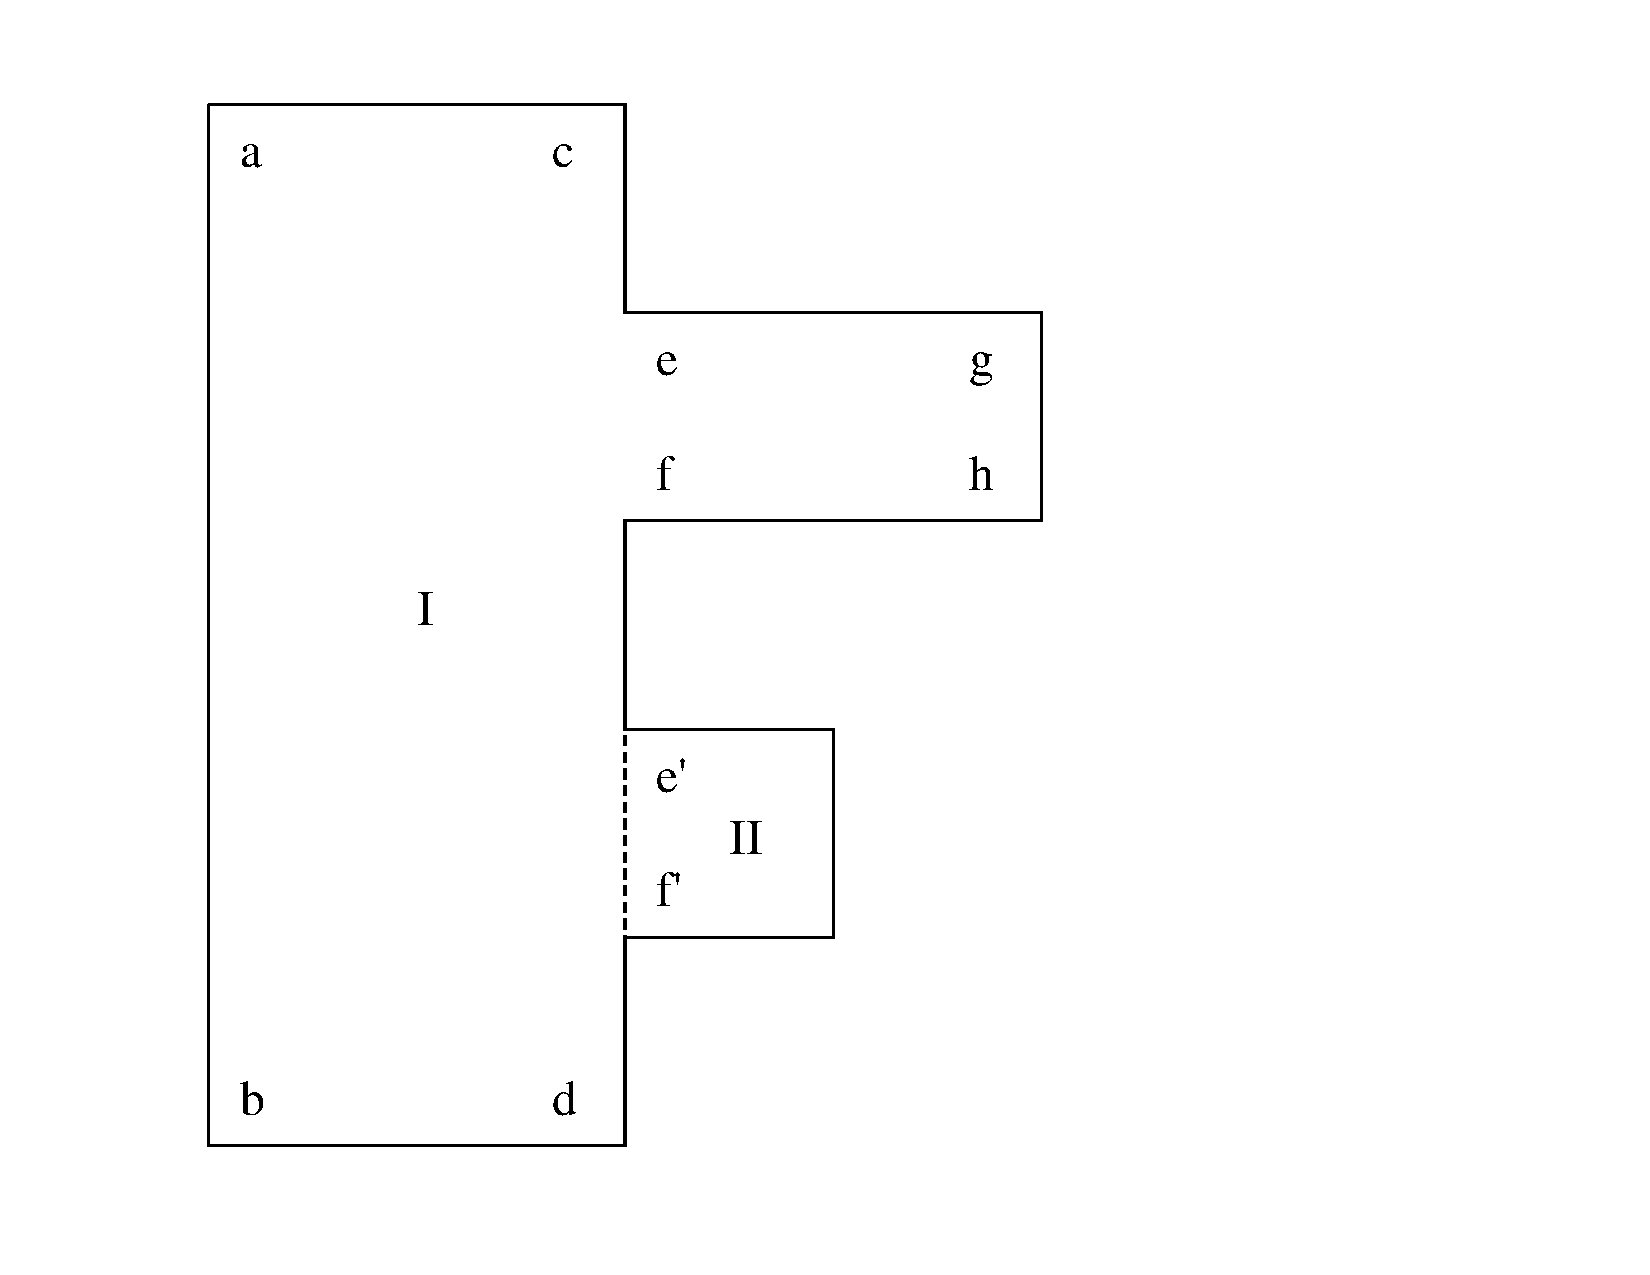
\includegraphics[keepaspectratio, height=4.0in, angle=0]{figs/covr1ack}
\caption[Pattern-search logic in used in COVR's subroutine
 matshd]{Pattern-search logic in subroutine matshd.}
\label{shade}
\end{figure}

As the plot option is presently coded, the entire correlation matrix
must reside in memory during the pattern-search operation just
described.

\subsection{Input Instructions for COVR}
\label{ssCOVR_inp}

As an aid to discussions of the user input to COVR, we list below the
input instructions that appear as comment cards at the beginning of the
current version of this module.  It is always advisable to consult the
comment-card instructions embedded in the version of the code actually
being used and not to rely on the instructions published in any
document, including this one.  Following the listing are further
remarks on several of the input items; the remarks supplement the
comment cards below.  See especially the lengthy discussion of the
parameters on Card 4.
\index{COVR!COVR input}
\index{input!COVR}

\small
\begin{ccode}

   !---input specifications (free format)---------------------------
   !
   !  card 1
   !     nin            input tape unit
   !     nout           output tape unit
   !                    (default=0=none)
   !     nplot          viewr output unit
   !                    (default=0=none)
   !
   !   ---cards 2, 2a, and 3a for nout.ne.0 only (plot option)
   !
   !  card 2
   !     icolor          select color or monochrome style
   !                       0=monochrome (uses cross hatching)
   !                       1=color background and contours
   !                       2=color background and contours plus
   !                         card 2' follows.
   !                       (default=0)
   !  card 2' (only when icolor=2)
   !     nlev,(tlev(i),i=1,nlev)
   !                     defines the number of correlation matrix
   !                     intervals and their boundaries.  Zero is
   !                     assumed as the lower limit of the first
   !                     boundary, but the User must specify unity
   !                     as the upper limit of the last boundary.
   !                     nlev is a positive integer .le. 9.
   !                     default values (when icolor=1) are:
   !                       6,0.001,0.1,0.2,0.3,0.6,1.0
   !  card 2a
   !     epmin          lowest energy of interest (default=0.)
   !  card 3a
   !     irelco         type of covariances present on nin
   !                    0/1=absolute/relative covariances
   !                    (default=1)
   !     ncase          no. cases to be run (maximum=40)
   !                    (default=1)
   !     noleg          plot legend option
   !                    -1/0/1=legend for first subcase only/
   !                    legend for all plots/no legends
   !                    (default=0)
   !     nstart         sequential figure number
   !                    0/n=not needed/first figure is figure n.
   !                    (default=1)
   !     ndiv           no. of subdivisions of each of the
   !                    gray shades (default=1)
   !
   !   ---cards 2b, 3b, and 3c for nout gt 0 (library option) only--
   !
   !  card 2b
   !     matype         output library matrix option
   !                    3/4=covariances/correlations
   !                    (default=3)
   !     ncase          no. cases to be run (maximum=40)
   !                    (default=1)
   !  card 3b
   !     hlibid         up to 6 characters for identification
   !  card 3c
   !     hdescr         up to 21 characters of descriptive
   !                    information
   !
   !   ---cards 4 for both options---
   !
   !  card 4
   !     mat            desired mat number
   !     mt             desired mt number
   !     mat1           desired mat1 number
   !     mt1            desired mt1 number
   !                    (default for mt, mat1 and mt1 are 0,0,0
   !                    meaning process all mts for this mat
   !                    with mat1=mat)
   !                    (neg. values for mt, mat1, and mt1 mean
   !                    process all mts for this mat, except for
   !                    the mt-numbers -mt, -mat1, and -mt1.  in
   !                    general, -n will strip both mt=1 and mt=n.
   !                    -4 will strip mt=1, mt=3, and mt=4, and
   !                    -62, for example, will strip mt=1, mt=62,
   !                    mt=63, ... up to and incl. mt=90.)
   !          repeat card 4 ncase times
   !
   ! note---if more than one material appears on the input tape,
   ! the mat numbers must be in ascending order.
   !
   !--------------------------------------------------------------------

\end{ccode}
\normalsize

\cword{icolor} \ldots\hspace{0.1in}This parameter is used to specify
creation of monochrome (cross-hatched) or color correlation matrix
plots.  Although the default setting is \cword{icolor}=0 (to produce
monochrome plots) the capabilities of modern printers and display
terminals makes creation of color plots the more common
option.  If \cword{icolor}=1 a default six-interval color pattern is
used when creating the correlation matrix; if \cword{icolor}=2 then
input card~2' is required where the user specfies the number of
color intervals (an integer, \cword{nlev}, where \cword{nlev} is a
positive non-zero integer $<$ 10) plus \cword{nlev} real numbers
that define the color boundaries, \cword{tlev(i)}, i=1,
\cword{nlev}.  \cword{tlev(\cword{nlev})} must be unity.  Users
are cautioned that use of too many intervals may require an
increase in the value of \cword{ipat} in \cword{subroutine matshd}.

\cword{epmin } \ldots\hspace{.1in}This parameter is used to eliminate
uninteresting energy regions from the correlation and standard
deviation plots, or to display high-energy regions with greater
resolution.

\cword{irelco } \ldots\hspace{.1in}This parameter must
match the value used in the \hyperlink{sERRORRhy}{ERRORR}
run that produced the covariances to be plotted.

\cword{ncase } \ldots\hspace{.1in}This is the number of cases, or
occurrences of Card 4.  See the discussion of input parameters
\cword{mat}, \cword{mt}, \cword{mat1}, and \cword{mt1} below.
Presently, \cword{ncase} is limited to 60.  Problems larger than this
can be run as a series of COVR jobs, each processing a batch of up to
60 cases.  See also the parameter \cword{nstart} below.

\cword{noleg } \ldots\hspace{.1in}``Legend'' here refers to the
gray-shading scale (key) as well as the figure caption.
\cword{noleg}=1 is used as a rough-draft mode to display plots
quickly.

\cword{nstart } \ldots\hspace{.1in}Unless \cword{nstart}=0, the plots
are assigned a sequential figure number, beginning at \cword{nstart},
and a list of figures is drawn on the final plot frame.

\cword{ndiv } \ldots\hspace{.1in}One gray-shade step equals 0.20 in
correlation magnitude if \cword{ndiv}=1.  Finer gradations are possible
with \cword{ndiv} greater than 1.  The plots appearing in the
\hyperlink{sERRORRhy}{ERRORR} section of this manual were
generated with \cword{ndiv}=2.

\cword{hlibid } \ldots\hspace{.1in}This is a 6-character string,
normally containing the name of the output covariance library.  It
is written on the header records present at the beginning of each
output data block.

\cword{hdescr } \ldots\hspace{.1in}This contains additional
information, for example, on where and when the library was produced;
it is also written on the data header records.

\cword{mat, mt, mat1, mt1 } \ldots\hspace{.1in}The information
contained in the output library or plot file is controlled by means of
these parameters on input Card 4.  If \cword{mt} is
positive, then a single covariance matrix for reaction
(\cword{mat,mt}) with reaction (\cword{mat1,mt1}) will be read from
\cword{nin} and processed.  On unit \cword{nin} (and, in the library
option, on unit \cword{nout}), the rapidly varying, or column,
index is the group index of (\cword{mat1,mt1}), and the slowly varying,
or row, index is the group index of (\cword{mat,mt}). ~If
\cword{mat1} is different from \cword{mat}, COVR will expect to find
separate materials (produced by separate
\hyperlink{sERRORRhy}{ERRORR} runs) for both
\cword{mat} and \cword{mat1} on \cword{nin}.  The \cword{mat} numbers
must occur on \cword{nin} in ascending order.  In the case of positive
\cword{mt}, the entries \cword{mat1}=0 and \cword{mt1}=0 are shorthand
for \cword{mat1}=\cword{mat} and \cword{mt1}=\cword{mt}, respectively.
If, on the other hand, \cword{mt} is zero, negative, or
defaulted, Card 4 becomes a kind of macro-instruction that
is expanded by subroutine \cword{expndo} into a request for many
(\cword{mt, mt1}) pairs, all  with \cword{mat1}=\cword{mat}.  If, for example,
Card 4 contains the entry

\small
\begin{ccode}

     MAT/

\end{ccode}
\normalsize

\noindent
or, equivalently,

\small
\begin{ccode}

     MAT 0 0 0/

\end{ccode}
\normalsize

\noindent
first the cross-section file, \cword{MF}$ = $\cword{3}, for material
\cword{MAT} is read from the input covariance tape on unit
\cword{nin} to obtain the list of reactions present.  Then, all
possible reaction combinations (\cword{mt, mt1}) are formed in ENDF
order.  Thus, for example, if the reactions present are \cword{MT}$ =
$\cword{1, 2, 3}, and \cword{16}, then the behavior of the code is the
same as if the following input were specified:

\small
\begin{ccode}

     MAT 1 0 1/
     MAT 1 0 2/
     MAT 1 0 3/
     MAT 1 0 16/
     MAT 2 0 2/
     MAT 2 0 3/
     MAT 2 0 16/
     MAT 3 0 3/
     MAT 3 0 16/
     MAT 16 0 16/

\end{ccode}
\normalsize

\noindent
Because of the clear labor-saving advantage of this feature, especially if
there are many reactions, enhancements have been added to permit its use
in the additional situation in which many, but not all, combinations are
desired.  As discussed in some detail in the input instructions, it is
possible to strip selected reactions out of the list before the
(\cword{mt, mt1}) combinations are formed.  For example, if the reactions
present are once again 1, 2, 3, and 16, then a Card 4 containing

\small
\begin{ccode}

     MAT -3/

\end{ccode}
\normalsize

\noindent
would produce the same output as the following three cards:

\small
\begin{ccode}

     MAT 2 0 2/
     MAT 2 0 16/
     MAT 16 0 16/

\end{ccode}
\normalsize

\noindent
The stripping of the higher inelastic levels, mentioned in the input
instructions, is useful because \hyperlink{sERRORRhy}{ERRORR}
automatically resets the
highest user-group energy to 20 MeV whenever \cword{IREAD}=0, and this
can result in the inclusion of unwanted high-threshold reactions on the
\hyperlink{sERRORRhy}{ERRORR} output file.

For one of several reasons, a requested reaction pair
(\cword{mat,mt; mat1,mt1}) may be absent from the COVR output.
The usual reason that this occurs is that the normal \cword{iread} option
for the \hyperlink{sERRORRhy}{ERRORR} module is \cword{iread}=0,
and this results in the generation of an output matrix for every
possible reaction-pair combination.  For those combinations that
do not occur in the ENDF evaluation, the
\hyperlink{sERRORRhy}{ERRORR} output matrix contains only
zeroes.  These null matrices are omitted at the COVR output stage,
in both the library and plot modes.

Additionally, in the plot mode, the correlations may be nonzero, but
everywhere less than \cword{0.2/ndiv} in absolute magnitude.  In this
case, the entire correlation plot would consist of a single blank region.
These rather uninteresting plots having small correlations are also
omitted from the plot file.  A final, similar category is the class of
``empty'' plots.  Because parallel lines to achieve a gray effect
when color is not used have limited resolution, there
is clearly some lower limit, for a given value of the correlation
magnitude, on the physical size of a region that can be sensibly shaded.
COVR does not attempt to shade regions that are smaller than this limit.
If a correlation matrix does contain some plottable data (magnitudes
exceeding \cword{0.2/ndiv}), but all plottable regions are smaller than
the size limit discussed above, then an empty plot will be generated on
the plot file.  As a convenience in discarding these empty plots at the
time a report is produced, no caption is written on such plots and the
figure number is not advanced.  Also, these plots are omitted from
the list of figures prepared at the end of a plot run.  (See the
discussion of user-input parameter \cword{nstart}.)

In the library mode, each omission of a requested, but null, matrix is
noted on the \cword{output} file with an informative diagnostic.  In the
plot mode, a summary table is printed at the end of the run to identify
all requested matrices that were omitted because they were null or
small, as well as those that were plotted, but empty.


\subsection{COVR Example Problem}
\label{ssCOVR_example1}

In this section we discuss the production of a particular COVR output
library, both to illustrate the input and as a supplement to the
general discussion of BOXER format libraries in  Section~\ref{ssCOVR_Boxer}.
In the \hyperlink{sERRORRhy}{ERRORR} chapter of this report
(the second input set in Section~\ref{ssERRORR_inp}),
we gave the complete NJOY input for producing a 7-reaction,
30-group covariance library in \hyperlink{sERRORRhy}{ERRORR}
output format for $^{12}$C.  By appending the following lines to
that input (just before the \cword{stop} card), one can produce,
in addition, a 2-reaction COVR output library in BOXER format.

\small
\begin{ccode}

     covr
     -23 24/
     3 3/
     '  LIB'/
     'MAT1306 COVR EXAMPLE'/
     1306 2 0 2/
     1306 2 0 4/
     1306 4 0 4/

\end{ccode}
\normalsize

\noindent
The resulting library occupies only 49 lines and is listed below.

%\begin{ccode}
\small
\begin{verbatim}
0    LIB-A- 30 MAT1306 COVR EXAMPLE  1306   2 1306   2  31 10  31  3   0  31   1
 1.390E-04 1.520E-01 4.140E-01 1.130E+00 3.060E+00 8.320E+00 2.260E+01 6.140E+01
 1.670E+02 4.540E+02 1.235E+03 3.350E+03 9.120E+03 2.480E+04 6.760E+04 1.840E+05
 3.030E+05 5.000E+05 8.230E+05 1.353E+06 1.738E+06 2.232E+06 2.865E+06 3.680E+06
 6.070E+06 7.790E+06 1.000E+07 1.200E+07 1.350E+07 1.500E+07 1.700E+07
 -1 -1 -1 -1 -1 -1 -1 -1 -1 -1 -1 -1 -1 -1 -1 -1 -1 -1 -1 -1 -1 -1 -1 -1 -1 -1
 -1 -1 -1 -1 -1
1    LIB-A- 30 MAT1306 COVR EXAMPLE  1306   2 1306   2  23 10  23  3   0  30   1
 4.739E+00 4.738E+00 4.735E+00 4.729E+00 4.712E+00 4.676E+00 4.579E+00 4.332E+00
 4.002E+00 3.619E+00 3.103E+00 2.477E+00 1.998E+00 1.820E+00 1.710E+00 2.256E+00
 1.447E+00 9.921E-01 8.223E-01 7.627E-01 8.631E-01 8.228E-01 8.845E-01
 -8 -1 -1 -1 -1 -1 -1 -1 -1 -1 -1 -1 -1 -1 -1 -1 -1 -1 -1 -1 -1 -1 -1
2    LIB-A- 30 MAT1306 COVR EXAMPLE  1306   2 1306   2  18 10  18  3   0  30   1
 2.000E-03 1.964E-03 4.583E-03 3.822E-03 4.583E-03 4.288E-03 3.730E-03 4.141E-03
 6.501E-03 1.011E-02 9.558E-03 9.981E-03 1.806E-02 1.854E-02 3.296E-02 3.760E-02
 4.255E-02 7.632E-02
 -9 -1 -5 -1 -1 -1 -1 -1 -1 -1 -1 -1 -1 -1 -1 -1 -1 -1
3    LIB-A- 30 MAT1306 COVR EXAMPLE  1306   2 1306   2  43 10  58  4   0  30   0
 4.000E-06 2.797E-06 3.856E-06 6.317E-06 4.613E-06 2.407E-06 1.229E-06 2.100E-05
 1.534E-05 8.000E-06 4.087E-06 1.461E-05 1.366E-05 2.100E-05 1.838E-05 9.004E-06
 1.391E-05 8.934E-06 1.715E-05 4.447E-06 4.227E-05 4.373E-05 2.446E-05 1.980E-05
 1.223E-05 1.022E-04 6.116E-05 4.048E-05 2.500E-05 9.136E-05 4.572E-05 9.962E-05
 6.641E-05 6.308E-05 3.260E-04 1.614E-04 3.437E-04 1.086E-03 4.250E-04 1.413E-03
 7.052E-04 1.811E-03 5.825E-03
  -9  -1 224  -1  -5  -1  -4  -1   9  -5  -1  -4  -1  79  -1  -1  13  -1  13  -1
  -1  11  -1  -1  10  -1  -1   9  -1  -1  -1  -1  -6  -1  -1  -1  -6  -1  -1   6
  -1  -1  -1   4  -1  -1   4  -1   4  -1  -2   1  -1  -1   1  -1   1  -1
3    LIB-A- 30 MAT1306 COVR EXAMPLE  1306   2 1306   4  38 10  47  4   0  30  30
-1.106E-04-4.897E-05-3.047E-05-2.164E-05-2.630E-05-2.337E-05-2.192E-05-2.261E-04
-1.001E-04-6.228E-05-4.423E-05-5.376E-05-4.777E-05-4.481E-05-1.441E-03-2.659E-04
-1.571E-04-1.210E-03-1.305E-03-4.021E-04-1.131E-03-6.462E-04-8.562E-04-2.261E-04
-1.001E-04-6.228E-05-1.922E-03-9.140E-04-8.121E-04-7.520E-04-3.040E-03-1.348E-03
-1.517E-03-3.460E-03-4.423E-05-5.376E-05-4.777E-05-1.044E-02
 623  -1  -1  -1  -1  -1  -1  -1  23  -1  -1  -1  -1  -1  -1  -1  53  -1  -1  -1
  27  -1  -1  -1  27  -1  -1  -1  27  -1  -1  -1  -1  -1  -1  27  -1  -1  -1  28
  -1  -1  27  -1  -1  -1  -1
1    LIB-A- 30 MAT1306 COVR EXAMPLE  1306   4 1306   4   7 10   8  3   0  30   1
 6.091E-02 2.478E-01 3.301E-01 4.310E-01 4.013E-01 4.306E-01 4.935E-01
 23 -1 -1 -1 -1 -1 -1 -1
2    LIB-A- 30 MAT1306 COVR EXAMPLE  1306   4 1306   4   7 10   8  3   0  30   1
 2.499E-01 1.085E-01 9.724E-02 9.806E-02 1.358E-01 1.263E-01 2.177E-01
 23 -1 -1 -1 -1 -1 -1 -1
3    LIB-A- 30 MAT1306 COVR EXAMPLE  1306   4 1306   4  28 10  29  4   0  30   0
 6.245E-02 7.530E-03 3.823E-03 1.154E-03 1.338E-03 1.211E-03 1.155E-03 1.176E-02
 2.311E-03 5.938E-04 6.451E-04 5.843E-04 5.578E-04 9.455E-03 1.887E-03 4.735E-04
 4.295E-04 4.106E-04 9.617E-03 1.872E-03 1.670E-03 3.033E-04 1.844E-02 5.214E-03
 3.493E-04 1.596E-02 5.253E-03 4.741E-02
 437  -1  -1  -1  -1  -1  -1  -1  -1  -1  -1  -1  -1  -1  -1  -1  -1  -1  -1  -1
  -1  -1  -1  -1  -1  -1  -1  -1  -1
\end{verbatim}
\normalsize
%\end{ccode}

Note that the header card at the start of each data block contains an
integer \cword{itype}, specifying the type of data contained in the
current block, a 12-character library name (``\cword{LIB-A- 30}'' in
this case), 21 characters of user-supplied descriptive information,
\cword{mat, mt, mat1, mt1}, and a set of 7 integers.  The meaning of
the various values of \cword{itype} is as follows: 0 = group
boundaries, 1 = cross sections, 2 = standard deviations, 3 =
covariances, and 4 = correlations.  The library name is generated within
COVR by adding either ``-A-" (for a covariance library) or
``-B-" (for a correlation library), together with the number of
energy groups, to the user-supplied library name \cword{hlibid}.  (The
\hyperlink{sERRORRhy}{ERRORR} input option \cword{ign}=3 used in
this example specifies a built-in 30-group structure).  The final
seven integers on the header card indicate the number and format
of the data values, the number and format of the control integers
(called {\it ``m''} and {\it ``-n''} in the discussion in
Section~\ref{ssCOVR_Boxer}), a data paging flag, and the
dimensions of the reconstructed data array, $C(i,j)$.

In order to clarify the process of reconstructing a full matrix from
data in BOXER format, we list in Section~\ref{ssCOVR_retrieval} a short
retrieval program, BOXR.  With very few modifications, this program could be
incorporated into a sensitivity analysis program, for example, to allow
direct access to covariance libraries\cite{COVFILS2} in this compact
format.  Alternatively, it could be used to translate COVR libraries
into other desired forms.  In any case, an examination of the retrieval
program should clarify the meaning of the various integer parameters on
the header cards in a COVR output library.

\subsection{Error Messages}
\label{ssCOVR_err}

\begin{description}
\begin{singlespace}

\item[\cword{error in covr***requested too many cases.}]~\par
  \cword{ncase} is limited to 40.  Note that a case refers to one
  input Card 4, which may request processing of either a single reaction
  pair or a whole series of reaction pairs.  See input instructions for
  Card 4 and the comments that follow.

\item[\cword{error in expndo***storage exceeded.}]~\par
  Should not occur since array space is allocated based upon known
  storage needs.

\item[\cword{error in corr***group structures do not agree.}]~\par
  This problem should not occur.

\item[\cword{error in covard***storage exceeded.}]~\par
  Should not occur since array space is allocated based upon known
  storage needs.

\item[\cword{error in covard***did not find file 77 subsection...}]~\par
  Requested reaction y of the current x-y pair is not found on \cword{nin}.

\item[\cword{error in trunc***bad data.}]~\par
  Either all cross sections are very small (less than
  \cword{xslim} = $10^{-4}$ barn) or \cword{epmin} is larger than
  the highest group boundary.

\item[\cword{error in matshd***ipat gt 99999.}]~\par
  Maximum number of correlation patterns is 99999.  Reduce \cword{ndiv} to
  1 or raise \cword{epmin} in order to reduce the complexity of the
  correlation plot.

\item[\cword{error in matshd***storage exceeded.}]~\par
  \cword{nwig}=2*(\cword{ixmax}+1)+600 words are available for storing the
  boundary curve of a constant-correlation region.  This will not be
  exceeded for any practical number of groups \cword{ixmax}.

\item[\cword{error in level***coefficient = --- out of range.}]~\par
  The absolute magnitude of a computed correlation coefficient is greater
  than 2.  The input covariance file may be faulty.

\item[\cword{error in finds***mat --- mf --- mt --- not on tape.}]~\par
  Requested reaction x of the current x-y pair is not found on \cword{nin}.

\item[\cword{error in press***storage exceeded.}]~\par
  This problem should not occur.

\item[\cword{error in press***matrix not symmetric....}]~\par
  Symmetric-matrix format is requested for a matrix that is asymmetric.
  This problem should not occur.

\item[\cword{error in setfor***nvf (= ---) or ncf (= ---) is illegal.}]~\par
  This problem should not occur.

\end{singlespace}
\end{description}

\subsection{Input/Output Units}
\label{ssCOVR_IO}

The following logical units are used:
\begin{description}
\begin{singlespace}

\item[10]   \cword{nin} in \cword{corr} and \cword{covard, nscr} in
other routines.  These units are used to extract either one or two (if
\cword{mat1}$\neq$\cword{mat}) materials from the input covariance
tape.

\item[11]   \cword{nscr1} in the plot mode.  These units are used
to document null and small covariance matrices and empty plots.

\item[11/12]  \cword{nscr1/nscr2} in the library mode.  In
\cword{covard}, the input covariances for the current reaction pair are
read from unit 10 and written to \cword{nscr2} (= 12).  If the output
library is to contain correlation coefficients (\cword{matype} = 4),
then in \cword{corr} the covariances are read from \cword{nscr2}, and
the calculated correlations are written to \cword{nscr1} (= 11).  If
output covariances are requested (\cword{matype} = 3), the value of
\cword{nscr1} is simply reset to \cword{nscr2} (= 12).  In either case,
\cword{press} reads the data from unit \cword{nscr1} and writes the
compressed data to \cword{nout}.

\item[20-99]   User's choice for \cword{nin} and \cword{nout}.

\end{singlespace}
\end{description}

\noindent
Unit 10 has the same mode as \cword{nin}.  Unit \cword{nout}, if used, is
always formatted.  Unit 11 is formatted in the plot option and it is binary
in the library option.  Unit 12, if used, is always binary.


\subsection {Retrieval Program for COVR Output Libraries}
\label{ssCOVR_retrieval}

\small
\begin {ccode}

      PROGRAM BOXR
C     ******************************************************************
C     FUNCTION OF PROGRAM.  READ DATA FROM UNIT NIN IN THE COMPRESSED
C     *BOXER* FORMAT PRODUCED BY THE COVR MODULE OF NJOY, AND LOAD THE
C     FULL, RECONSTRUCTED MATRIX INTO C(I,J).  THEN WRITE THE RESULT ON
C     UNIT NOUT IN HIGH-TO-LOW ENERGY ORDER.  FAILURE TO FIND A
C     REQUESTED DATA SET RESULTS IN AN ERROR STOP.
C
C       ITYPE   DATA TYPE REQUESTED,
C                 = -1, TO WRITE A TABLE OF CONTENTS OF NIN, IN THE
C                   FORMAT OF BOXR INPUT INSTRUCTIONS, ON UNIT NTAB.
C                 = 0, FOR GROUP BOUNDARIES,
C                 = 1, FOR CROSS SECTIONS,
C                 = 2, FOR STANDARD DEVIATIONS,
C                 = 3, FOR COVARIANCE MATRIX,
C                 = 4, FOR CORRELATION MATRIX, OR (IF MT1 IS ZERO)
C                   TRANSFER MATRIX FROM COVFILS2.
C       ITYPEH  VALUE OF ITYPE ON CURRENT DATA HEADER CARD.
C
C      (MAT,MT,MAT1,MT1)     REQUESTED REACTION PAIR.
C      (MATH,MTH,MAT1H,MT1H) CURRENT REACTION PAIR.
C      (XVAL(IV),IV=1,NVAL)  DATA VALUE ARRAY IN THE *BOXER* FORMAT.
C       NVMAX                MAXIMUM ALLOWABLE VALUE OF NVAL.
C      (ICON(IC),IC=1,NCON)  CONTROL-PARAMETER ARRAY IN *BOXER* FORMAT.
C       NCMAX                MAXIMUM ALLOWABLE VALUE OF NCON.
C
C       I       ROW INDEX OF MATRIX C(I,J), NORMALLY THE ENERGY GROUP
C                 OF THE REACTION (MAT,MT).
C       NROW    NUMBER OF ROWS IN C(I,J).
C       NROWH   VALUE OF NROW ON DATA HEADER CARD.
C       NROWM   CONTINUATION FLAG, = 0 FOR FINAL DATA BLOCK OF CURRENT
C                 REACTION PAIR.
C       J       COLUMN INDEX OF C(I,J), FOR MATRIX DATA THE ENERGY GROUP
C                 OF THE REACTION (MAT1,MT1), = 1 FOR VECTORS.
C       NCOL    NUMBER OF COLUMNS IN C(I,J).
C       NCOLH   VALUE OF NCOL ON DATA HEADER CARD, = 0 IF C(I,J) IS A
C                 SYMMETRIC MATRIX REPRESENTED IN THE *BOXER* FORMAT BY
C                 JUST THE UPPER RIGHT TRIANGLE (J.GE.I).
C       NGMAX   MAXIMUM ALLOWABLE VALUE OF NROW AND NCOL.
C     ******************************************************************
      DIMENSION IVFT(3), ICFT(3), IA(9), IB(9)
      DIMENSION C(200,200), CR(200), XVAL(880), ICON(900)
      DATA NGMAX /200/, NVMAX /880/, NCMAX /900/, IDASH /4H----/
      DATA NINPUT /5/, NIN /20/, NOUT /21/, NTAB /22/, IZERO /0/
C
C     ***READ USER-SUPPLIED REACTION-TYPE AND MAT-MT INFORMATION.
   10 READ (NINPUT,190) ITYPE,MAT,MT,MAT1,MT1
C     INPUT IS TERMINATED BY ENTERING (0,0).
      IF (ITYPE.GE.0.AND.MAT.EQ.0) STOP
C
C     ***RETRIEVE REQUESTED DATA FROM UNIT NIN.
   20 READ (NIN,210,END=900) ITYPEH,(IA(K),K=1,9),MATH,MTH,MAT1H,MT1H
     1 ,NVAL,NVF,NCON,NCF,NROWM,NROWH,NCOLH
C
C     ***IN COVFILS2, ITYPEH=9 IS USED AS A TERMINATOR.
   30 IF (ITYPEH.EQ.9) GO TO 900
      IF (ITYPE.EQ.-1.AND.MATH.EQ.0) MATH=1
      IF (ITYPE.EQ.-1.AND.IA(2).NE.IDASH)
     1 WRITE (NTAB,190) ITYPEH,MATH,MTH,MAT1H,MT1H
      IF (NVAL.GT.NVMAX) STOP 3
      IF (NCON.GT.NCMAX) STOP 4
C     SET FORMATS, THEN READ BOXER DATA.
      CALL SETFOR (NVF,NCF,NOUT,IVFT,ICFT)
      IF (NVAL.GT.0) READ (NIN,IVFT) (XVAL(K),K=1,NVAL)
      IF (NCON.GT.0) READ (NIN,ICFT) (ICON(K),K=1,NCON)
C     TEST IF THESE ARE THE DESIRED DATA.  FOR THE GROUP BOUNDARIES
C     ONLY, THE VALUES MATH, MTH, MAT1H, AND MT1H ON THE HEADER CARD
C     ARE IGNORED.  FOR ITYPE=1 OR 2, MAT1H AND MT1H ARE IGNORED.
C     FOR MATRIX DATA, ITYPE=3 OR 4, A COMPLETE MATCH IS REQUIRED.
      IF (ITYPEH.NE.ITYPE) GO TO 20
      IF (ITYPE.EQ.0) GO TO 40
      IF (MATH.NE.MAT.OR.MTH.NE.MT) GO TO 20
      IF (ITYPE.EQ.1.OR.ITYPE.EQ.2) GO TO 40
      IF (MAT1H.NE.MAT1.OR.MT1H.NE.MT1) GO TO 20
C     INITIALIZE
   40 NX=0
      I=1
      ISTART=1
      J=0
   50 NROW=NROWH
      NCOL=NCOLH
      IV=0
      NSYM=0
      IF (NCOL.EQ.0) NSYM=1
      IF (NCOL.EQ.0) NCOL=NROW
      IF (NROW.GT.NGMAX.OR.NCOL.GT.NGMAX) GO TO 910
C
C     ***LOAD DATA FROM XVAL INTO C(I,J) AS DIRECTED BY ICON.
      DO 110 IC=1,NCON
      IF (ICON(IC).LT.0) GO TO 60
      IF (ICON(IC).EQ.0) STOP 6
      NLOAD=ICON(IC)
      GO TO 70
   60 NLOAD=-ICON(IC)
      IV=IV+1
      IF (IV.GT.NVAL) STOP 7
      CLOAD=XVAL(IV)
   70 CONTINUE
      DO 100 N=1,NLOAD
      J=J+1
      IF (J.LE.NCOL) GO TO 80
C     START NEW ROW
      I=I+1
      IF (I.GT.NROW) STOP 10
      J=1
      IF (NSYM.EQ.1) J=I
   80 IF (ICON(IC).LE.0) GO TO 90
      CLOAD=0.
      IF (I.GT.ISTART) CLOAD=C(I-1,J)
   90 C(I,J)=CLOAD
      NX=NX+1
      IF (NSYM.EQ.0.OR.I.EQ.J) GO TO 100
      C(J,I)=CLOAD
      NX=NX+1
  100 CONTINUE
  110 CONTINUE
      IF (NROWM.EQ.0) GO TO 120
C     READ IN NEW PAGE OF DATA FROM NIN
      IF (J.NE.NCOL) STOP 11
      READ (NIN,210) ITYPEH,(IB(K),K=1,9),MATH,MTH,MAT1H,MT1H,NVAL,NVF
     1 ,NCON,NCF,NROWM,NROWH,NCOLH
      CALL SETFOR (NVF,NCF,NOUT,IVFT,ICFT)
      IF (NVAL.GT.0) READ (NIN,IVFT) (XVAL(K),K=1,NVAL)
      IF (NCON.GT.0) READ (NIN,ICFT) (ICON(K),K=1,NCON)
      ISTART=I+1
      GO TO 50
  120 CONTINUE
C     FINISHED LOADING C(I,J)
      IF (NX.NE.NROW*NCOL) STOP 12
C
C     ***WRITE C(I,J) TO NOUT IN HIGH-TO-LOW ENERGY ORDER.
      WRITE (NOUT,220)
      WRITE (NOUT,210) ITYPEH,(IA(K),K=1,9),MATH,MTH,MAT1H,MT1H,NVAL,NVF
     1 ,NCON,NCF,NROWM,NROWH,NCOLH
      IF (NCOL.EQ.1) GO TO 150
      DO 140 I=1,NROW
      IR=NROW+1-I
C     IN COVFILS2, TRANSFER MATRICES ARE ALREADY IN HIGH-TO-LOW ORDER
      IF (ITYPE.EQ.4.AND.MT1.EQ.0) IR=I
      DO 130 J=1,NCOL
      JR=NCOL+1-J
      IF (ITYPE.EQ.4.AND.MT1.EQ.0) JR=J
  130 CR(J)=C(IR,JR)
  140 WRITE (NOUT,200) (CR(L),L=1,NCOL)
      GO TO 10
  150 DO 160 I=1,NROW
      IR=NROW+1-I
  160 CR(I)=C(IR,1)
      WRITE (NOUT,200) (CR(K),K=1,NROW)
      GO TO 10
C
C     ***PRINT ERROR MESSAGES.
  900 IF (ITYPE.NE.-1) WRITE (NOUT,901) ITYPE,MAT,MT,MAT1,MT1
  901 FORMAT (/50H ***ERROR IN BOXR***CANNOT FIND ITYPE,MAT,MT,MAT1,
     1 ,5HMT1 =,5I5)
      IF (ITYPE.EQ.-1) WRITE(NTAB,190) IZERO,IZERO
      STOP
  910 WRITE (NOUT,911) NGMAX
  911 FORMAT (/45H ***ERROR IN BOXR*** NUMBER OF GROUPS EXCEEDS,I4)
      STOP
C
  190 FORMAT (5I6)
  200 FORMAT (1P8E10.3)
  210 FORMAT (I1,A3,8A4,2(I5,I4),2(I4,I3),3I4)
  220 FORMAT (///)
      END
      SUBROUTINE SETFOR (NVF,NCF,NOUT,IVFT,ICFT)
C     ******************************************************************
C     SET *BOXER* INPUT/OUTPUT FORMATS.
C     ******************************************************************
      DIMENSION IFT(3,14), IVFT(3), ICFT(3)
      DATA IFT /4H(80I,4H1)  ,4H    ,4H(40I,4H2)  ,4H    ,4H(26I,4H3)  ,
     1 4H    ,4H(20I,4H4)  ,4H    ,4H(16I,4H5)  ,4H    ,4H(13I,4H6)  ,4H
     2    ,4H(11F,4H7.4),4H    ,4H(10F,4H8.5),4H    ,4H(1P8,4HE9.2,4H)
     3 ,4H(1P8,4HE10.,4H3)  ,4H(1P7,4HE11.,4H4)  ,4H(1P6,4HE12.,4H5)  ,4
     4 H(1P6,4HE13.,4H6)  ,4H(1P5,4HE14.,4H7)  /
C
      IF (NVF.LT.7.OR.NVF.GT.14) GO TO 900
      IF (NCF.LT.1.OR.NCF.GT.6) GO TO 900
C
C     ***SET FORMATS
      DO 10 I=1,3
      IVFT(I)=IFT(I,NVF)
   10 ICFT(I)=IFT(I,NCF)
      RETURN
C
C     ERROR MESSAGE
  900 WRITE (NOUT,901) NVF,NCF
  901 FORMAT (/28H ***ERROR IN SETFOR***NVF (=,I3,11H) OR NCF (=,I3,13H)
     1 IS ILLEGAL.)
      STOP
      END

\end{ccode}
\normalsize

\cleardoublepage


\section{MODER}
\label{sMODER}

\hypertarget{sMODERhy}{The}
MODER\index{MODER|textbf} module is used to convert ENDF\index{ENDF},
PENDF\index{PENDF}, and GENDF\index{GENDF} tapes from the
NJOY blocked-binary mode\index{blocked binary} to formatted mode
(ASCII on modern computers), and {\it vice versa}. It can
also be used to copy data from one logical unit to another without
change of mode, or to make a new tape containing selected materials
from one or more  ENDF, PENDF, or GENDF tapes.  MODER handles
ENDF-4 through ENDF-6 formats, plus special-purpose formats developed
for NJOY, such as the
\hyperlink{sGROUPRhy}{GROUPR}\index{GROUPR} and
\hyperlink{sERRORRhy}{ERRORR}\index{ERRORR}
output formats.

This chapter describes the MODER module in NJOY2016.0.

\subsection{Code Description}
\label{ssMODER_description}

The main subroutine \cword{moder} is exported by the
module \cword{modem}\index{modules!modem@{\ty modem}}.
At the beginning of execution, MODER rewinds the output tape \cword{nout}.
Additionally, each time a new input tape \cword{nin} is specified,
that unit is rewound.  MODER then processes \cword{nin} one file at a time,
either for all materials on \cword{nin}, or optionally (see following
section) for a single specified material. As each file is identified,
the main program calls a subroutine dedicated to that file.  Each
subroutine makes the series of calls to \cword{contio}, \cword{listio},
etc., that is appropriate to that file.

If \cword{nin} and \cword{nout} are of opposite sign, then mode conversion
is performed automatically by the utility I/O subroutines.  If
\cword{nin} and \cword{nout} have the same sign, then no mode conversion
is performed; runs of this type can be used simply to make an extra copy
of the input tape or to retrieve selected materials without mode change.
Only a little more than one page of scratch storage is needed, so there
are no limitations on which tapes can be processed.

\subsection{Input Instructions}
\label{ssMODER_inp}

As an aid to discussions of the user input to MODER, the input
instructions that appear as comment cards at the beginning of the
current version of this module are listed below.  Since code changes
are possible, it is always advisable to consult the comment-card
instructions contained in the version of the code actually being
used before proceeding with an actual calculation.
\index{MODER!MODER input}
\index{input!MODER}

\newpage
\small
\begin{ccode}

   !---input specifications (free format)---------------------------
   !
   ! card 1       unit numbers
   !      nin     input unit
   !      nout    output unit
   !
   !  a positive unit is coded (mode 3).
   !  a negative unit is blocked binary (njoy mode).
   !
   !  note: abs(nin) ge 1 and le 19 is a flag to select various
   !        materials from one or more input tapes, with or
   !        without mode conversion.  the kind of data to be
   !        processed is keyed to nin as follows:
   !             nin=1, for endf or pendf input and output,
   !                 2, for gendf input and output,
   !                 3, for errorr-format input and output.
   !
   !      cards 2 and 3 for abs (nin) ge 1 and le 19 only.
   !
   ! card 2
   !      tpid    tapeid for nout.  66 characters allowed
   !              (delimited with ', ended with /)
   ! card 3
   !      nin     input unit
   !              terminate moder by setting nin=0
   !      matd    material on this tape to add to nout
   !-------------------------------------------------------------------

\end{ccode}
\normalsize

\noindent
The contents of \cword{nin} and \cword{nout} are positive or negative
logical unit numbers, with absolute magnitudes normally in the
range 20-99, inclusive.  Positive unit numbers refer to formatted tapes,
and negative unit numbers refer to blocked-binary tapes.  No other
input is required to copy or convert the entire contents of the data
file on unit \cword{nin}, writing the results to unit \cword{nout}.

A positive value of \cword{nin} in the range 1-3 is used as a
trigger to specify that the data to be copied or converted are not
the contents of a single tape, but, instead, they are selected materials
from one or more input tapes.  The type of data to be processed
(ENDF/PENDF {\it vs.} GENDF {\it vs.}
\hyperlink{sERRORRhy}{ERRORR}-format) is keyed to the value of
\cword{nin}, as detailed in the instructions above.  If \cword{nin}
is in the range 1-3, and only in this case, additional input is
supplied to specify (on card 2) the tape-identification information
to be written on the first record of the output tape and to specify
(on card 3) both the \cword{mat}-numbers of the materials to be included and
the logical units where each of the desired materials are to
be found.  Note that the slash terminating the Hollerith information
on card 2 is required. In the case of GENDF processing of a material
\cword{matd}, which is present on the specified input tape at a series of
temperatures, a single card 3
causes the retrieval of all temperatures.
Card 3 is repeated as many times as needed, and input is terminated
with a card containing 0/.

\subsection{Sample Input}
\label{ssMODER_sampleinp}

It is good practice to convert the mode of the ENDF/B tape before
proceding with any NJOY run.  The time spent in MODER is normally
much less than the time saved by the subsequent modules.  The required
input for this is extremely simple.  In this first example, an ENDF-formatted
file, designated ``tape20" is copied to a binary-formatted file designated
``tape21".  This file is subsequently used as input to
\hyperlink{sRECONRhy}{RECONR}.

\small
\begin{ccode}

   moder
   20 -21/
   reconr
   -21 -22/
   ...

\end{ccode}
\normalsize

For older versions of ENDF/B, the released ``tapes'' usually
contained multiple materials.  In the following example we specify
that a single material, 1305, be extracted from ``tape20" and
written to ``tape21".  Subsequent use of ``tape21" will be more
efficient since only the material of interest is on that tape.

\small
\begin{ccode}

   moder
   1 -21/
   'B-10'/
   20 1305/
   0/
   reconr
   -21 -22/
   ...

\end{ccode}
\normalsize

The final example (taken from one of the standard sample problems)
shows the use of MODER to prepare a special multimaterial ENDF tape
for a covariance calculation involving the 5 primary fissionable isotopes.
Since, in this particular example problem, the resonance region is of
no interest, a copy of the ENDF serves as the PENDF for later modules.
Mount ENDF Tape 515, 516, and 555 on units 20, 21, and 22.

\small
\begin{ccode}

   moder
   1 -23/
   'endf/b-v nubar covariance materials'/
   20 1380/
   20 1381/
   21 1390/
   22 1395/
   22 1398/
   20 1399/
   0/
   moder
   -23 -24/
   group
   -23 -24 0 25/
   ...

\end{ccode}
\normalsize

\noindent
The second moder run copies the ENDF file to use as a PENDF file
for \hyperlink{sGROUPRhy}{GROUPR}.

\subsection{Error Messages}
\label{ssMODER_msg}

\begin{description}
\begin{singlespace}

\item[\cword{error in moder***endf materials must be in ascending order}] ~\par
  This is a problem with the material ordering for the input tape.

\item[\cword{message from moder---mat nnnn not found on gendf tape}] ~\par
  Check the \cword{matd} value on input card 3 and make sure that
  the correct input tape was mounted.

\item[\cword{error in moder***this material is not a gendf material}] ~\par
  Input file contains an illegal mixture of data,
  namely, an initial GENDF
  material, followed by the indicated non-GENDF \cword{mat}.

\item[\cword{error in moder***input is not an errorr output tape}] ~\par
  User has requested \hyperlink{sERRORRhy}{ERRORR}-format
  processing, but input data file is not a
  \hyperlink{sERRORRhy}{ERRORR}-format tape.

\item[\cword{error in moder***input is not an endf or pendf tape}] ~\par
  User has specified \cword{nin}=1 on card 1, thereby requesting selective
  multitape ENDF or PENDF processing, but input data file on the unit
  \cword{nin} specified on card 3 is not an ENDF/PENDF file.

\item[\cword{error in moder***input is not an endf tape}] ~\par
  See comments above.

\item[\cword{error in moder***input is not a gendf tape}] ~\par
  User has requested GENDF processing, but input data file is not a
  GENDF tape.

\item[\cword{error in moder***conversion not coded for mf=nn}] ~\par
  There is an illegal or unrecognizable \cword{mf} value on \cword{nin}.

\item[\cword{error in moder***should have found send card}] ~\par
  MODER expected the end of a section but found actual data.
  The listed data display the contents of the last card
  read.  Input data file may be bad or may use a format not yet implemented.

\item[\cword{error in moder***illegal covariance mf=nn}] ~\par
  ERRORR-format file is missing the required \cword{mf}=3.
  ENDF and PENDF tapes must be \cword{mat} ordered.

\item[\cword{error in file1***bad LFC in mt=458.}] ~\par
  There is a bad value for the \cword{LFC} value in \cword{mf}=1 \cword{mt}=458.
  Only 0 or 1 are allowed.

\item[\cword{error in file1***bad LO in mt=460.}] ~\par
  There is a bad value for the \cword{LO} value in \cword{mf}=1 \cword{mt}=460.
  Only 0 or 1 are allowed.

\item[\cword{error in file1***illegal mt}] ~\par
  Only the standard \cword{mt}=451 to 458 and 460 are allowed in File 1.

\item[\cword{error in file2***illegal mt}] ~\par
  Only the standard \cword{mt}=151 and the NJOY special values of \cword{mt}=152
  and 153 are allowed in File 2.

\item[\cword{error in file5***illegal lf}] ~\par
  The File 5 \cword{lf} value is outside the legal range 1-12.

\item[\cword{error in file6***illegal ltt}] ~\par
  This message comes from the branch used for ENDF-5 format
  or for thermal data generated by the
  \hyperlink{sTHERMRhy}{THERMR} module.
  Check the format of the File 6 sections.

\item[\cword{error in file6***illegal endf6 law}] ~\par
  This message comes from the branch used for ENDF-6 tapes.
  Check the values for the law parameter in the sections of File 6.
  Only law values 0 to 7 are allowed. In the case of fission, negative law values
  are also allowed.

\item[\cword{error in file6***illegal endf6 law for mt=nnn}] ~\par
  This message comes from the branch used for ENDF-6 tapes.
  Check the values for the law parameter in the corresponding section of File 6.
  Negative law values are only allowed for fission (mt=18).

\item[\cword{error in file7***bad NS in mt4.}] ~\par
  The number of non-principal scattering atom types NS cannot be larger than 3.

\item[\cword{error in file7***illegal mt=nnn}] ~\par
  Only \cword{mt}=2 and \cword{mt}=4 are allowed in File 7 for the ENDF-6
  format.

\item[\cword{error in file7***illegal value of lthr=n}] ~\par
  Only values of 1 or 2 are allowed for \cword{lthr} in ENDF-6.

\item[\cword{error in file12***bad LO in mt=460.}] ~\par
  There is a bad value for the \cword{LO} value in \cword{mf}=1 \cword{mt}=460.
  Only 0, 1 or 2 are allowed.

\item[\cword{error in file15***illegal lf}] ~\par
  Only \cword{lf}=1 and the special lanl format \cword{lf}=2 are allowed

\item[\cword{error in file32***illegal value of ndigit}] ~\par
  There is a bad value for the \cword{NDIGIT} value in \cword{mf}=32.
  Only 0 or 2 to 6 are allowed.

\item[\cword{error in file32***illegal value of lcomp}] ~\par
  There is a bad value for the \cword{LCOMP} value in \cword{mf}=32.
  Only 0, 1 or 2 are allowed.

% The following error messages are in the source code but ISR is no longer referenced
% the ENDF manual. These might be obsolete.
% \item[\cword{error in file32***unknown isr}] ~\par
% \item[\cword{error in file32***isr>0 not supported for lrf=7}] ~\par

\end{singlespace}
\end{description}

\cleardoublepage


\section{DTFR}
\label{sDTFR}

\hypertarget{sDTFRhy}{This}
module is used to prepare libraries for discrete-ordinates
\index{DTFR|textbf}
\index{DTF-IV}
\index{S$_{\rm N}$ transport}
transport codes that accept the format designed for the S$_{\rm N}$ code
DTF-IV\cite{DTF}.  As this was one of the early discrete-ordinats
codes, many newer S$_{\rm N}$ and
diffusion codes allow DTF format as an input option.  DTFR also
contains a simple plotting capability for providing a quick look
at its output.  DTFR was the first output module written for the
NJOY system, and it has been largely superseded by the MATXS/TRANSX
\index{MATXS/TRANSX} system.  But DTFR is still useful for some purposes
because of its simplicity.

This chapter describes the DTFR module in NJOY2016.0.

\subsection{Transport Tables}
\label{ssTTables}

Transport tables\index{transport tables} in DTF format are organized to
mirror the structure of the data inside a discrete-ordinates transport code.
\index{discrete-ordinates transport}  These codes start with the highest
energy group and work downward.  (The conventional order for group indices
is to increase as energy decreases.)  Therefore, for each group $g$, the
data required are the reaction cross sections for group $g$ and the
scattering cross sections to $g$ from other groups $g'$.  Each data element
is said to occupy a ``position'' in the table for group $g$. The
organization is shown in Table~\ref{positions}.

\begin{table}[h]
\caption{Organization of Data for One Group
  in a Transport Table}
\begin{center}
\begin{tabular}{cl}
Position & Meaning \\ \hline
  1      & edit cross sections \\
$\cdots$ &   (if any) \\
 \cword{iptotl-3}& last special edit  \\
 \cword{iptotl-2}& particle-balance absorption \\
 \cword{iptotl-1}& fission neutron production \\
 \cword{iptotl}  & total cross section \\
 \cword{iptotl}+1& upscatter $g{\leftarrow}g'\:(g'{>}g)$ \\
 $\cdots$&  (if any) \\
 \cword{ipingp}  & ingroup scattering $g{\leftarrow}g$ \\
 $\cdots$& downscatter $g{\leftarrow}g'\:(g'<g)$ \\
 \cword{itabl}   & end of table \\ \hline
\end{tabular}
\end{center}
\label{positions}
\end{table}

The basic table consists of the three standard edits, namely,
particle balance absorption ($\sigma_a$), fission neutron
production cross section ($\bar{\nu}\sigma_f$), and total cross
section ($\sigma_t$).  These standard edits are followed by the
group-to-group scattering cross sections.  If desired, the standard
edits can be preceded by \cword{iptotl-3} special edits, which can be
used in the transport code to calculate various responses of the system
(for example, heating, activation, or gas production).  If
\cword{iptotl} is the position of the total cross section, the
positions of the three standard edits will be \cword{iptotl-2},
\cword{ipingp-1}, and \cword{iptotl}, respectively.  The positions
of the special edits (if \cword{iptotl>3}) will be
1, 2, \ldots \cword{iptotl-3}.

Most transport tables describe only downscatter.  In such cases, the
position of the ingroup element is \cword{ipingp}=\cword{iptotl}+1.  Position
\cword{iptotl}+1 would contain $\sigma_{g{\leftarrow}(g{-}1)}$, and so
on.  If thermal upscatter is present, the \cword{nup} upscatter
cross sections are between the total cross section element and the
ingroup element.  Therefore, position \cword{iptotl-1} contains
$\sigma_{g{\leftarrow}(g{+}1)}$, and so on.  The position parameters
must satisfy the following conditions:
\begin{center}
     \cword{iptotl} $\ge$ 3 ~, and\\
     \cword{ipingp} = \cword{iptotl} + \cword{nup} + 1~.
\end{center}
The number of positions for a group is called the table length.
A full table will have the table length given by
\begin{center}
     \cword{itabl} = \cword{iptotl-3} + 3 + \cword{nup} + \cword{ng  ,}
\end{center}
where \cword{ng} is the total number of groups in the set.  Table
lengths can be truncated in some cases.  If this is done correctly,
the important cross sections will be conserved, and valid results
can still be obtained.

An example of a transport table is given in Table~\ref{ttable}.
This table was generated with DTFR for ENDF/B-VI $^{235}$U (\cword{mat}=9228).
It contains three special edits: the (n,2n) cross section, the fission
cross section, and the radiative capture cross section.  These are
followed by the three standard edits, and then by the ingroup
scattering for group 1.  Since this is the highest energy group,
there is no downscatter to this group from groups above, and the
rest of the positions are filled with zeros.  Group 2 starts on
line 8 with the six edit cross sections.  The seventh number is
the ingroup cross section, and the eighth is the scattering from
group 1 to group 2.  Continuing to lines 14 and 15, there are now
two downscatter elements:  two to three and one to three.
Note that there is an entire table for each Legendre order, and
that each table has a header card that describes its contents.
The ellipses were added to mark removed lines.

\newpage

\begin{table}[t]\small
\caption{Example of a Transport Table with Internal Edits}
%\begin{ccode}
\begin{verbatim}

 IL= 1 TABLE 30 GP 36 POS, MAT= 9228 IZ= 1 TEMP= 3.00000E+02
  3.2597E-01  2.0823E+00  6.1629E-04  1.3965E+00  9.7755E+00  5.9989E+00
  3.1734E+00  0.0000E+00  0.0000E+00  0.0000E+00  0.0000E+00  0.0000E+00
  0.0000E+00  0.0000E+00  0.0000E+00  0.0000E+00  0.0000E+00  0.0000E+00
  0.0000E+00  0.0000E+00  0.0000E+00  0.0000E+00  0.0000E+00  0.0000E+00
  0.0000E+00  0.0000E+00  0.0000E+00  0.0000E+00  0.0000E+00  0.0000E+00
  0.0000E+00  0.0000E+00  0.0000E+00  0.0000E+00  0.0000E+00  0.0000E+00
  4.9950E-01  2.0532E+00  1.1756E-03  1.4681E+00  9.1321E+00  5.8659E+00
  3.0495E+00  1.1523E-01  0.0000E+00  0.0000E+00  0.0000E+00  0.0000E+00
  0.0000E+00  0.0000E+00  0.0000E+00  0.0000E+00  0.0000E+00  0.0000E+00
  0.0000E+00  0.0000E+00  0.0000E+00  0.0000E+00  0.0000E+00  0.0000E+00
  0.0000E+00  0.0000E+00  0.0000E+00  0.0000E+00  0.0000E+00  0.0000E+00
  0.0000E+00  0.0000E+00  0.0000E+00  0.0000E+00  0.0000E+00  0.0000E+00
  6.8192E-01  1.8830E+00  1.5668E-03  1.1928E+00  8.0521E+00  5.7877E+00
  2.9838E+00  8.2484E-02  3.1214E-02  0.0000E+00  0.0000E+00  0.0000E+00
 ...
 IL= 2 TABLE 30 GP 36 POS, MAT= 9228 IZ= 1 TEMP= 3.00000E+02
  0.0000E+00  0.0000E+00  0.0000E+00  0.0000E+00  0.0000E+00  0.0000E+00
  2.8003E+00  0.0000E+00  0.0000E+00  0.0000E+00  0.0000E+00  0.0000E+00
  0.0000E+00  0.0000E+00  0.0000E+00  0.0000E+00  0.0000E+00  0.0000E+00
  0.0000E+00  0.0000E+00  0.0000E+00  0.0000E+00  0.0000E+00  0.0000E+00
  0.0000E+00  0.0000E+00  0.0000E+00  0.0000E+00  0.0000E+00  0.0000E+00
  0.0000E+00  0.0000E+00  0.0000E+00  0.0000E+00  0.0000E+00  0.0000E+00
  0.0000E+00  0.0000E+00  0.0000E+00  0.0000E+00  0.0000E+00  0.0000E+00
  2.5972E+00  3.8535E-02  0.0000E+00  0.0000E+00  0.0000E+00  0.0000E+00
  0.0000E+00  0.0000E+00  0.0000E+00  0.0000E+00  0.0000E+00  0.0000E+00
  0.0000E+00  0.0000E+00  0.0000E+00  0.0000E+00  0.0000E+00  0.0000E+00
  0.0000E+00  0.0000E+00  0.0000E+00  0.0000E+00  0.0000E+00  0.0000E+00
  0.0000E+00  0.0000E+00  0.0000E+00  0.0000E+00  0.0000E+00  0.0000E+00
  0.0000E+00  0.0000E+00  0.0000E+00  0.0000E+00  0.0000E+00  0.0000E+00
  2.4730E+00  2.3851E-02  7.4855E-03  0.0000E+00  0.0000E+00  0.0000E+00
 ...
 IP= 1 TABLE 30 GP 12 POS, MAT= 9228 IZ= 1 TEMP= 3.00000E+02
  0.0000E+00  0.0000E+00  1.1808E-02  2.0992E-02  2.4928E-02  5.7726E-02
  6.0219E-01  1.8328E+00  5.5365E+00  7.5176E+00  1.0018E+01  2.0404E+00
  0.0000E+00  0.0000E+00  1.0938E-02  1.9445E-02  2.4306E-02  5.8998E-02
  5.7158E-01  1.7441E+00  5.2857E+00  7.2063E+00  9.5514E+00  1.9537E+00
  0.0000E+00  0.0000E+00  8.6352E-03  1.5352E-02  2.6314E-02  7.8974E-02
  5.3190E-01  1.6485E+00  5.0937E+00  7.1114E+00  9.1307E+00  1.9158E+00
  0.0000E+00  0.0000E+00  5.0549E-03  8.9865E-03  2.9371E-02  1.0974E-01
  4.6950E-01  1.4973E+00  4.7871E+00  6.9512E+00  8.4624E+00  1.8534E+00
 ....

\end{verbatim}
%\end{ccode}
\label{ttable}
\end{table}

The last table in this example describes the photon production
matrix.  There are 30 neutron groups and 12 photon groups.  The photon
group index replaces the position index used in the neutron tables.
Therefore, the first 12 numbers in this table correspond to photon
production from neutron group 1.  The photon groups are arranged in
order of decreasing energy.

The header lines at the start of each table in this example give
the Legendre order, number of groups, number of positions,
MAT number, $\sigma_0$ number, and temperature.

DTFR will also produce a variant of the transport tables that was used
for Los Alamos libraries in years past.  These are sometimes called
``CLAW Libraries'' after the CLAW-III and CLAW-IV libraries available
from the Radiation Safety Information Computational Center (RSICC)
\index{RSICC} at the Oak Ridge National Laboratory.  Although CLAW-IV
uses a version of this format, it was actually generated using MATXS
cross sections and the TRANSX code\cite{CLAW4,TRANSX}.
\index{CLAW library!CLAW-III}
\index{CLAW library!CLAW-IV}
\index{RSICC}
\index{MATXS/TRANSX}
The key feature of the CLAW tables is that the edits are removed
from their normal position at the beginning of each group in the
transport table and written out on separate lines.  The format
specified a particular list of reactions (see Table~\ref{predef}) that
is defined using data statements in DTFR.  In addition, thermal upscatter
is not allowed in this format.  An example of this style of transport
table is given in Table~\ref{ctable}.  Note that eye-readable identifiers
were added to the right-hand edge of each card by DTFR.  The card labels
contain the first two letters of the material name, the reaction name or
the Legendre order, and a sequence number.  The format of the header
lines at the start of each table is different from the last example.
The quantity in parentheses on the ``EDIT XSEC'' card is groups by
number of edit reactions.  For the neutron tables, it is table length
by groups.  For the gamma table, it is gamma groups by neutron groups.

%\begin{table}\footnotesize
\begin{table}\small
%\begin{longtable}{cccc}
\caption{Predefined Edits for DTFR}
%\endfirsthead
%\caption{Predefined Edits for DTFR (cont.)}
%\endhead
%    \hline
%    \multicolumn{4}{r}{\emph{Continued}}
%\endfoot
%    \hline
%\endlastfoot
\label{predef}
\begin{center}
\begin{tabular}{cccc}
   Reaction Name & Position & Reaction &  Multiplicity     \\ \hline
    \cword{els} &     1   &     2    &    1  \\
    \cword{ins} &     2   &     4    &    1  \\
    \cword{n2n} &     3   &    16    &    1  \\
                &     3   &     6    &    1  \\
                &     3   &     7    &    1  \\
                &     3   &     8    &    1  \\
                &     3   &     9    &    1  \\
    \cword{n3n} &     4   &    17    &    1  \\
    \cword{ngm} &     5   &   102    &    1  \\
    \cword{nal} &     6   &   107    &    1  \\
     \cword{np} &     7   &   103    &    1  \\
   \cword{fdir} &     8   &    19    &    1  \\
    \cword{nnf} &     9   &    20    &    1  \\
   \cword{n2nf} &    10   &    21    &    1  \\
   \cword{ftot} &    11   &    18    &    1  \\
     \cword{nd} &    12   &   104    &    1  \\
     \cword{nt} &    13   &   105    &    1  \\
   \cword{nhe3} &    14   &   106    &    1  \\
    \cword{n2p} &    15   &   111    &    1  \\
    \cword{npa} &    16   &   112    &    1  \\
   \cword{nt2a} &    17   &   113    &    1  \\
   \cword{nd2a} &    18   &   114    &    1  \\
    \cword{n2a} &    19   &   108    &    1  \\
    \cword{n3a} &    20   &   109    &    1  \\
    \cword{nnd} &    21   &    32    &    1  \\
  \cword{nnd2a} &    22   &    35    &    1  \\
  \cword{nnhe3} &    23   &    34    &    1  \\
    \cword{nna} &    24   &    22    &    1  \\
   \cword{n2na} &    25   &    24    &    1  \\
   \cword{nn3a} &    26   &    23    &    1  \\
   \cword{n3na} &    27   &    25    &    1  \\
    \cword{nnp} &    28   &    28    &    1  \\
   \cword{nn2a} &    29   &    29    &    1  \\
  \cword{n2n2a} &    30   &    30    &    1  \\
    \cword{nnt} &    31   &    33    &    1  \\
  \cword{nnt2a} &    32   &    36    &    1  \\
    \cword{n4n} &    33   &    37    &    1  \\
   \cword{n3nf} &    34   &    38    &    1  \\
    \cword{chi} &    35   &   470    &    1  \\
   \cword{chid} &    36   &   471    &    1  \\
    \cword{nud} &    37   &   455    &    1  \\
    \cword{phi} &    38   &   300    &    1  \\
  \cword{theat} &    39   &   301    &    1  \\
                &    39   &   443    &    0  \\
  \cword{kerma} &    40   &   443    &    1  \\
  \cword{tdame} &    41   &   444    &    1  \\
   \cword{nusf} &    42   &     1    &    1  \\
   \cword{totl} &    43   &   452    &    1  \\ \hline
\end{tabular}
\end{center}
\end{table}
%\end{longtable}

\begin{table}\small
\caption{Example of DTFR Transport Tables Using Separate Edits}
%\begin{ccode}
\begin{verbatim}
 U235       EDIT XSEC ( 30X 48) PROC BY NJOY1  ON 05/03/90
  3.03110E+00 2.85141E+00 2.75464E+00 2.66464E+00 2.87622E+00 3.56158E+00U2  ELS
  4.43195E+00 4.38571E+00 3.94779E+00 3.53864E+00 3.34261E+00 3.61868E+00U2  ELS
  4.74566E+00 6.13164E+00 7.65700E+00 9.34710E+00 1.08466E+01 1.16438E+01U2  ELS
  1.19400E+01 1.28024E+01 1.32190E+01 1.31520E+01 1.29202E+01 1.30545E+01U2  ELS
  1.27990E+01 1.19229E+01 1.32489E+01 1.41192E+01 1.47783E+01 1.54225E+01U2  ELS
  3.78514E-01 4.17166E-01 4.61638E-01 5.44816E-01 8.11127E-01 1.37822E+00U2  INS
  2.20958E+00 2.30405E+00 2.34199E+00 2.28404E+00 2.14540E+00 1.90879E+00U2  INS
  1.60448E+00 1.29695E+00 9.63151E-01 4.00064E-01 4.54497E-02 3.03043E-03U2  INS
  1.87467E-06 7.26072E-08 0.00000E+00 0.00000E+00 0.00000E+00 0.00000E+00U2  INS
  0.00000E+00 0.00000E+00 0.00000E+00 0.00000E+00 0.00000E+00 0.00000E+00U2  INS
  3.25966E-01 4.99502E-01 6.81925E-01 8.22064E-01 6.05949E-01 3.47278E-01U2  N2N
  8.86188E-03 0.00000E+00 0.00000E+00 0.00000E+00 0.00000E+00 0.00000E+00U2  N2N
  0.00000E+00 0.00000E+00 0.00000E+00 0.00000E+00 0.00000E+00 0.00000E+00U2  N2N
  ...
 U235   L=0 N-N TABLE ( 33X 30)
  1.39646E+00 9.77549E+00 5.99892E+00 3.17345E+00 0.00000E+00 0.00000E+00U2 0
  0.00000E+00 0.00000E+00 0.00000E+00 0.00000E+00 0.00000E+00 0.00000E+00U2 0
  0.00000E+00 0.00000E+00 0.00000E+00 0.00000E+00 0.00000E+00 0.00000E+00U2 0
  0.00000E+00 0.00000E+00 0.00000E+00 0.00000E+00 0.00000E+00 0.00000E+00U2 0
  0.00000E+00 0.00000E+00 0.00000E+00 0.00000E+00 0.00000E+00 0.00000E+00U2 0
  0.00000E+00 0.00000E+00 0.00000E+00 1.46808E+00 9.13206E+00 5.86594E+00U2 0
  3.04950E+00 1.15234E-01 0.00000E+00 0.00000E+00 0.00000E+00 0.00000E+00U2 0
  0.00000E+00 0.00000E+00 0.00000E+00 0.00000E+00 0.00000E+00 0.00000E+00U2 0
  ...
 U235   L=1 N-N TABLE ( 33X 30)
  0.00000E+00 0.00000E+00 0.00000E+00 2.80033E+00 0.00000E+00 0.00000E+00U2 1
  0.00000E+00 0.00000E+00 0.00000E+00 0.00000E+00 0.00000E+00 0.00000E+00U2 1
  0.00000E+00 0.00000E+00 0.00000E+00 0.00000E+00 0.00000E+00 0.00000E+00U2 1
  0.00000E+00 0.00000E+00 0.00000E+00 0.00000E+00 0.00000E+00 0.00000E+00U2 1
  0.00000E+00 0.00000E+00 0.00000E+00 0.00000E+00 0.00000E+00 0.00000E+00U2 1
  0.00000E+00 0.00000E+00 0.00000E+00 0.00000E+00 0.00000E+00 0.00000E+00U2 1
  2.59724E+00 3.85346E-02 0.00000E+00 0.00000E+00 0.00000E+00 0.00000E+00U2 1
  0.00000E+00 0.00000E+00 0.00000E+00 0.00000E+00 0.00000E+00 0.00000E+00U2 1
  ...
 U235   L=0 N-P TABLE ( 12X 30)
  0.00000E+00 0.00000E+00 1.18077E-02 2.09916E-02 2.49277E-02 5.77264E-02U2 0
  6.02189E-01 1.83282E+00 5.53653E+00 7.51757E+00 1.00182E+01 2.04037E+00U2 0
  0.00000E+00 0.00000E+00 1.09379E-02 1.94453E-02 2.43062E-02 5.89981E-02U2 0
  5.71583E-01 1.74411E+00 5.28569E+00 7.20630E+00 9.55138E+00 1.95373E+00U2 0
  0.00000E+00 0.00000E+00 8.63521E-03 1.53515E-02 2.63136E-02 7.89737E-02U2 0
  5.31904E-01 1.64847E+00 5.09371E+00 7.11139E+00 9.13067E+00 1.91577E+00U2 0
  0.00000E+00 0.00000E+00 5.05490E-03 8.98652E-03 2.93715E-02 1.09745E-01U2 0
  ....

\end{verbatim}
%\end{ccode}
\label{ctable}
\end{table}

\subsection{Data Representations}
\label{ssDataRep}

The data stored into the transport tables are obtained from
\hyperlink{sGROUPRhy}{GROUPR}\index{GROUPR}.  Since
all the scattering matrix reactions are
kept separate in the multigroup processing, it is necessary to add
them up to compute the DTF scattering matrix.  They are obtained from
the sections with \cword{mf}=6 on the input GENDF\index{GENDF} tape.  Similarly,
all the photon production matrices have to be added up to obtain the
final DTF photon production table.  These sections have \cword{mf}=16.

\newpage
The standard edit called particle-balance absorption is used in
discrete-ordinates transport codes to calculate the balance table.
The most fundamental definition for this quantity is
\begin{equation}
   \sigma_{a,g} = \sigma_{t,g} - \displaystyle\sum_{g'}
      \sigma_{s,g'{\leftarrow}g}\,\,.
\label{abs}
\end{equation}
The total cross section is obtained from \cword{mf}=3, \cword{mt}=1
on the input GENDF
tape.  The scattering matrix is obtained by adding all the matrix
reactions found in File 6 on the input tape.  The absorption edit
is often written in the form
\begin{equation}
   \sigma_{a,g} = \sigma_{\gamma,g} + \sigma_{f,g}
         - \sigma_{n2n,g}\,\,,
\end{equation}
which is good up to the threshold for other multiparticle reactions.
Because of the presence of the (n,2n) term, the $\sigma_a$ parameter
is not equal to the real neutron absorption for high-energy groups.
In fact, it is often negative.

The next standard edit is used to compute the fission neutron
production rate when constructing a fission source.  It is used
together with a fission spectrum, which can be included in the
specials edits (see below). The fission contributions from the GENDF
tape are complicated.  First, the prompt fission matrix may be given in
\cword{mt}=18 (total fission), or in the partial fission reactions
\cword{mt}=19, \cword{mt}=20, \cword{mt}=21, and \cword{mt}=38, which
stand for (n,f), (n,n$'$f),
(n,2nf), and (n,3nf).  Second, each of these matrices may take
advantage of the fact that the shape of the fission spectrum
is constant at low energies.  Thus, fission can be represented
using single fission $\chi^{LE}_g$ vector with this shape at low energies,
with an accompanying fission neutron production cross section
$\sigma^{LE}_{Pfg}$ at low energies, and with a rectangular fission
matrix $\sigma^{HE}_{g,g{\rightarrow}g'}$ at high energies.  The
third complication is the presence of delayed fission neutron emission.
The delayed neutron yield $\bar{\nu}^D_g$ is retrieved from
\cword{mf}=3, \cword{mt}=455,
and the delayed neutron spectrum $\chi^D_g$ is obtained by adding up
the spectra for the time groups in \cword{mf}=5, \cword{mt}=455.  The following
equation shows how these separate terms are combined into the
steady-state fission neutron production edit:
\begin{equation}
   \bar{\nu}^{SS}_g\sigma_{fg}=\displaystyle
      \sum_{g'}\sigma^{HE}_{fg{\rightarrow}g'}
     +\sigma^{LE}_{Pfg} + \bar{\nu}^D_g\sigma_{fg} \,\,.
\label{ssnu}
\end{equation}
The associated steady-state fission spectrum is given by
\begin{equation}
   \chi^{SS}_{g'}= \frac{\displaystyle\sum_g\sigma^{HE}_{fg{\rightarrow}g'}
      \phi_g + \chi^{LE}_{g'}\sum_g\sigma^{LE}_{Pfg}\phi_g
       +\chi^D_{g'}\sum_g\bar{\nu}^D_g\sigma_{fg}\phi_g}
         {\rm NORM} \,\,,
\label{sschi}
\end{equation}
\vspace{1 pt}

\noindent
where NORM is the quantity that will normalize the spectrum, namely,
the sum of the numerator over all $g'$.

The total cross section is read directly from \cword{mf}=3, \cword{mt}=1.  No
transport corrections are made.  The normal convention for libraries made with
DTFR in the past was to supply P$_4$ tables and let the application
code construct transport-corrected P$_3$ tables if it wanted them.

A flexible scheme is provided for constructing special edit
cross sections.  Each position can contain any of the cross sections
available in File 3 of the GENDF tape, or a position can contain
a combination of several cross sections weighted by multiplicities.
For example, the ENDF/B-IV evaluation for $^{12}$C contains the two
reactions (n,$\alpha$) (in \cword{mf}=3, \cword{mt}=107) and (n,n$'$)3$\alpha$
(in \cword{mf}=3, \cword{mt}=91).  To obtain the helium production
cross section, it is only necessary to request an edit made up as follows:
\begin{center}
   1 $\times$ MT107 $+$ 3 $\times$ MT91~.
\end{center}

\noindent
Most of the reactions for these special edits are requested by giving
their ENDF MT numbers.  The following special MT values are used to
request some special quantities:

\begin{center}
\begin{tabular}{cl}
  Special MT & Meaning \\ \hline
     300    &  weighting flux (from \cword{mf}=3, \cword{mt}=1) \\
     455    &  delayed neutron yield (\cword{mf}=3, \cword{mt}=455) \\
     470    &  steady-state spectrum (see Eq.~\ref{sschi}) \\
     471    &  delayed neutron spectrum (\cword{mf}=5, \cword{mt}=455) \\ \hline
\end{tabular}
\end{center}
\vspace{1 pt}
See Section~\ref{ssDTFR_inp} on user input for more details.

DTFR can also construct transport tables suitable for calculations
in the thermal range.  These tables allow for upscatter, and the
user can specify that bound scattering cross sections be used in
the thermal range instead of the normal static elastic scattering
reaction.  The NJOY thermal capabilities are described in more
detail in the
\hyperlink{sTHERMRhy}{THERMR}\index{THERMR} and
\hyperlink{sGROUPRhy}{GROUPR}\index{GROUPR} sections
of this report.  In brief, NJOY can provide thermal scattering
cross sections and matrices for any material treated as a free gas in
thermal equilibrium (a Maxwell-Boltzmann distribution), or it can provide
data for a number of important moderator materials whose scattering
laws $S(\alpha,\beta)$ are available in the ENDF/B-VII libraries.
These thermal ``materials'' look like different reactions for
the dominant scattering isotope after being processed by
\hyperlink{sGROUPRhy}{GROUPR}.
Table~\ref{dtherm} lists the different binding states that are available
for ENDF/B-VII and the MT numbers used to request them.  Materials
like ``H in H$_2$O'' give the scattering for the principal scattering
isotope only; the other isotope should be treated using free-gas
scattering.  There is an exception:  benzene was evaluated as
a complete molecule, and the results were renormalized to be used
with the cross section for the dominant isotope $^{1}$H.
Therefore, this material should be used with the density
corresponding to the dominant isotope, and no thermal contribution from
the other isotope should be included at all (set both \cword{mti} and
\cword{mtc} to zero).

\begin{table}\small
\caption[Thermal Reactions Available to DTFR]{Thermal Reactions
   Available to DTFR when using the ENDF/B-VII.0 Thermal Evaluations}
\begin{center}
\begin{tabular}{ccl}
  MTI  &  MTC  &  Thermal Binding Condition \\ \hline
  221  &       &  free gas \\
  222  &       &  H in H$_2$O \\
  223  &  224  &  H in polyethylene (CH$_2$)  \\
  225  &  226  &  H in ZrH  \\
  227  &       &  Benzene \\
  228  &       &  D in D$_2$O \\
  229  &  230  &  C in graphite \\
  231  &  232  &  Be metal \\
  233  &  234  &  Be in BeO  \\
  235  &  236  &  Zr in ZrH \\
  237  &  238  &  O in BeO \\
  239  &  240  &  O in UO$_2$ \\
  241  &  242  &  U in UO$_2$ \\
  243  &  244  &  Al metal \\
  245  &  246  &  Fe metal \\ \hline
\end{tabular}
\end{center}
\label{dtherm}
\end{table}

As described in more detail in the subsection on user input, DTFR
has an input parameter called \cword{ntherm} that specifies the
number of incident-energy groups to be treated using thermal
cross sections; this parameter determines the breakpoint between
the thermal treatment and the normal static treatment.  DTFR subtracts
the static elastic cross section (\cword{mt}=2) from both the total and
absorption edits in this group range, and it adds the \cword{mti}
and \cword{mtc} cross sections to these positions.  Similarly, it
omits the contributions from the \cword{mt}=2 matrix for these
final-energy groups, and it adds in the contributions from
\cword{mti} and \cword{mtc}.  The user is free to use a number of
upscatter positions less than \cword{ntherm}.  The code will truncate
the table in a way that preserves the total thermal scattering
cross section.

\subsection{Plotting}
\label{ssDTFR_Plot}

Plots of the output data from a formatting program like DTFR are useful
in two ways: first, they provide a nice summary of the library and help
its users to understand the trends in the data easily, and second,
they are helpful in quality control as an aid to finding errors in
processing.  This versions replaces the old-style plotting from the
original version of DTFR with a nicer system making use of the NJOY
VIEWR module to produce attractive Postscript plots.

\begin{figure}[bp]\centering
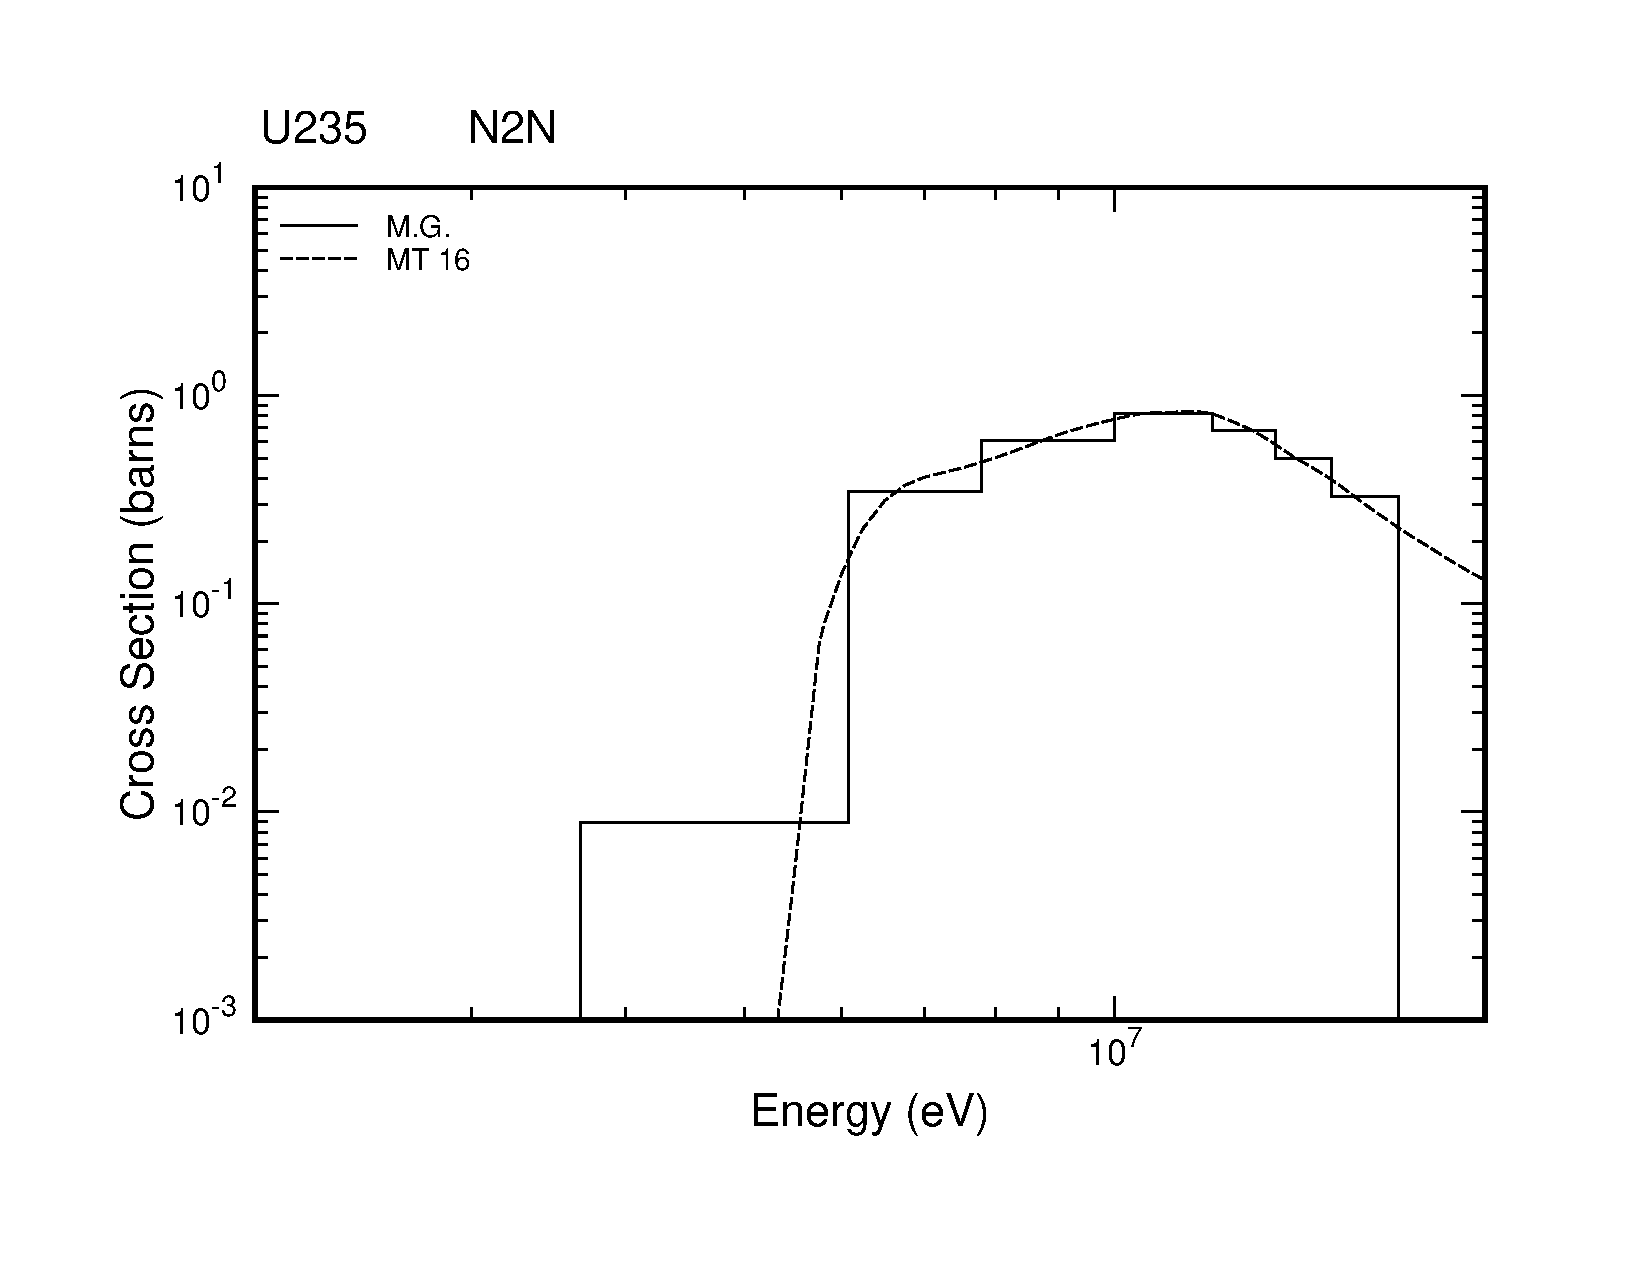
\includegraphics[keepaspectratio, height=3.0in, angle=0]{figs/dtfr1ack}
\caption[DTFR cross section plot example]{An example of DTFR plotting for
 the (n,2n) reaction of ENDF/B-VI $^{235}$U.  This plot was prepared using
 \cword{ifilm=1} and in-table edits.  All the threshold reactions are shown
 using the same energy range to make comparisons easy.}
\label{sing1}
\end{figure}

DTFR automatically makes two-dimensional log-log graphs for all the
special edit positions and the three standard edit positions.  If
available (see \cword{npend}), pointwise cross sections are plotted
on the same frame as the group cross sections.  If the multigroup
cross section is a combination of several reactions, the pointwise
cross sections for all of the components are plotted.  An example
of this will be found below.  DTFR also prepares three-dimensional
isometric projections of the P$_0$ scattering matrix and the P$_0$
photon-production table.  The user can request that one reaction
be plotted per page, or that four reactions be drawn on the same
page.  Examples of these plots are given in
Figures~\ref{sing1}--\ref{four}.

\begin{figure}[hp]\centering
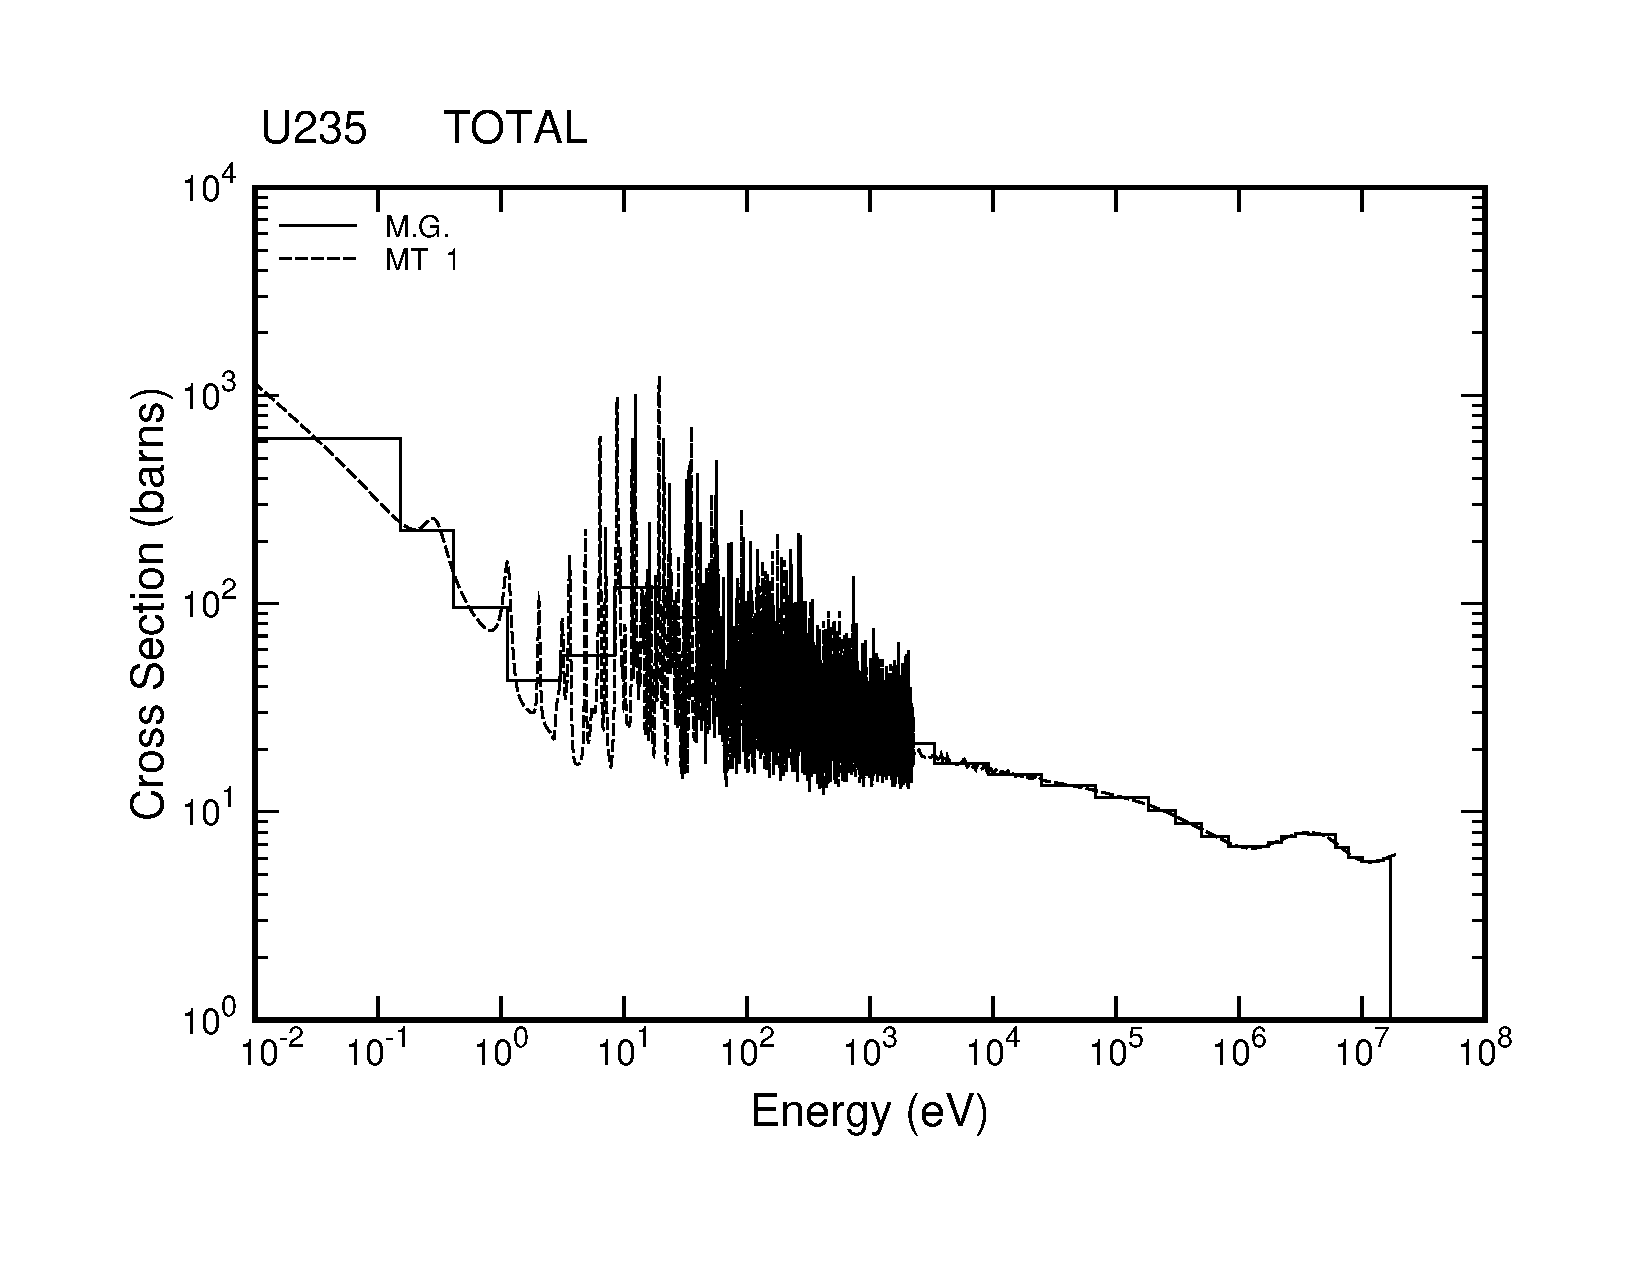
\includegraphics[keepaspectratio, height=3.2in, angle=0]{figs/dtfr2ack}
\caption[DTFR cross section plot example, expanded energy range]{This
 is the total cross section for ENDF/B-VI $^{235}$U from the same run as
 the previous plot.  The energy range from $1{\times}10^{-5}$ eV to
 $1{\times}10^{-2}$ eV was removed to expand the rest of the energy scale.}
\label{sing2}
\end{figure}

\begin{figure}[hp]\centering
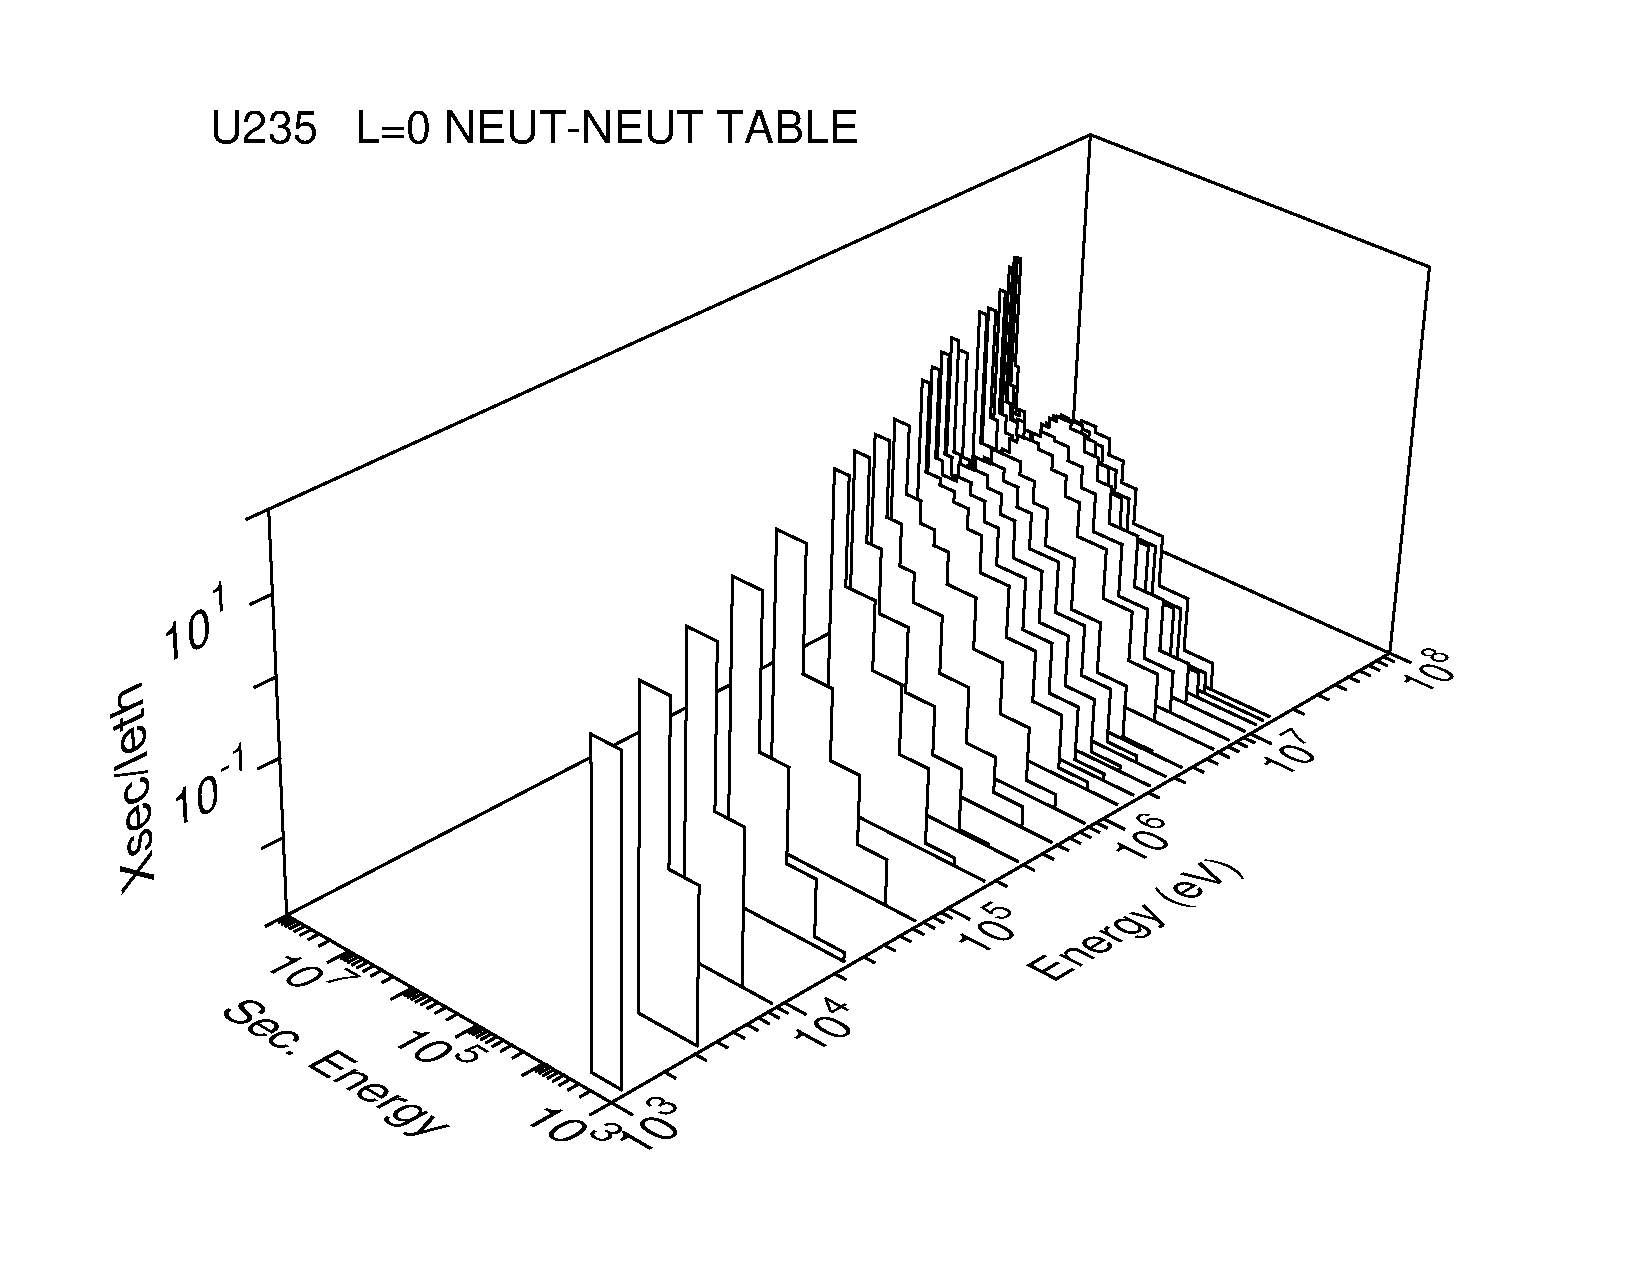
\includegraphics[keepaspectratio, height=3.2in, angle=0]{figs/dtfr3ack}
\caption[DTFR scattering matrix plot example]{This plot shows the P$_0$
 scattering matrix for ENDF/B-VI $^{235}$U by incident and secondary energy.}
\label{sing3}
\end{figure}

\begin{figure}[t]\centering
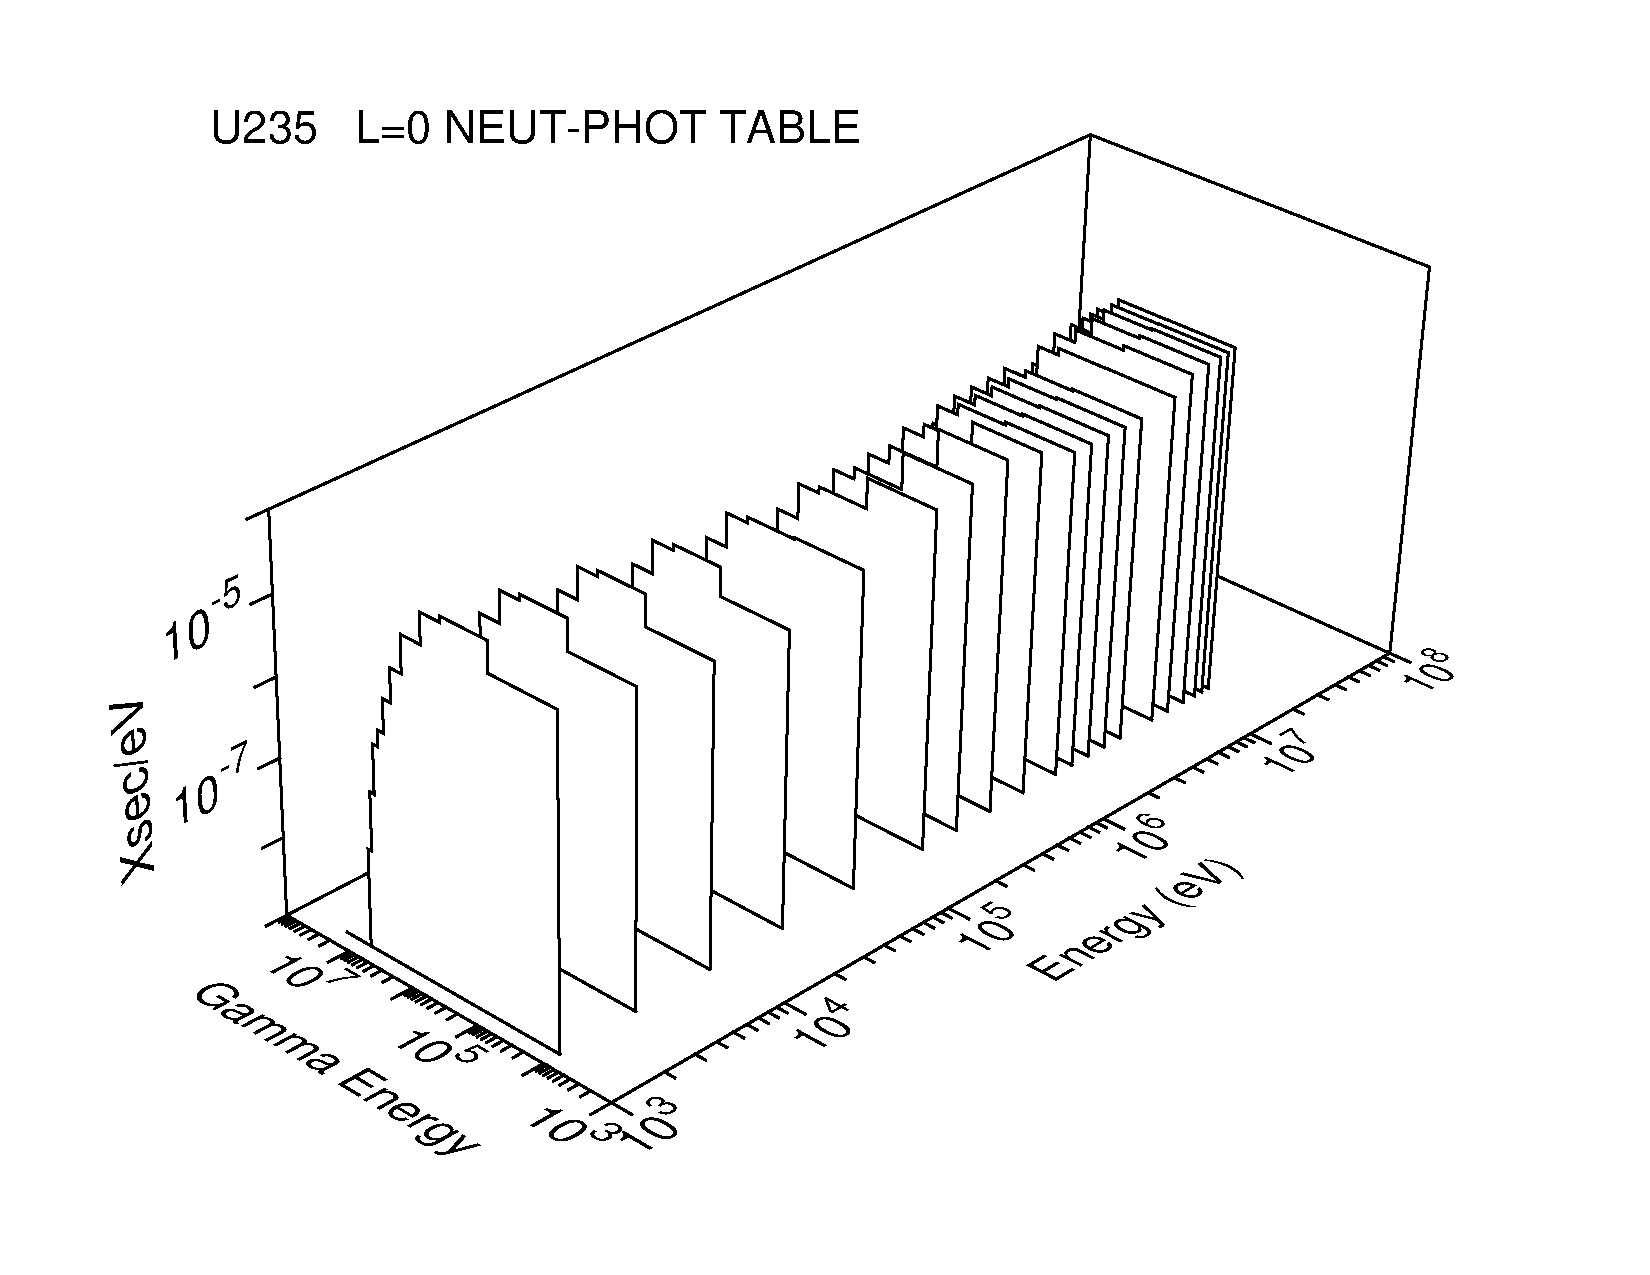
\includegraphics[keepaspectratio, height=3.2in, angle=0]{figs/dtfr4ack}
\caption[DTFR photon production matrix plot example]{The 30${\times}$12 P$_0$
 photon production matrix for $^{235}$U is plotted versus neutron energy
 and photon energy.}
\label{sing4}
\end{figure}

\begin{figure}[b]\centering
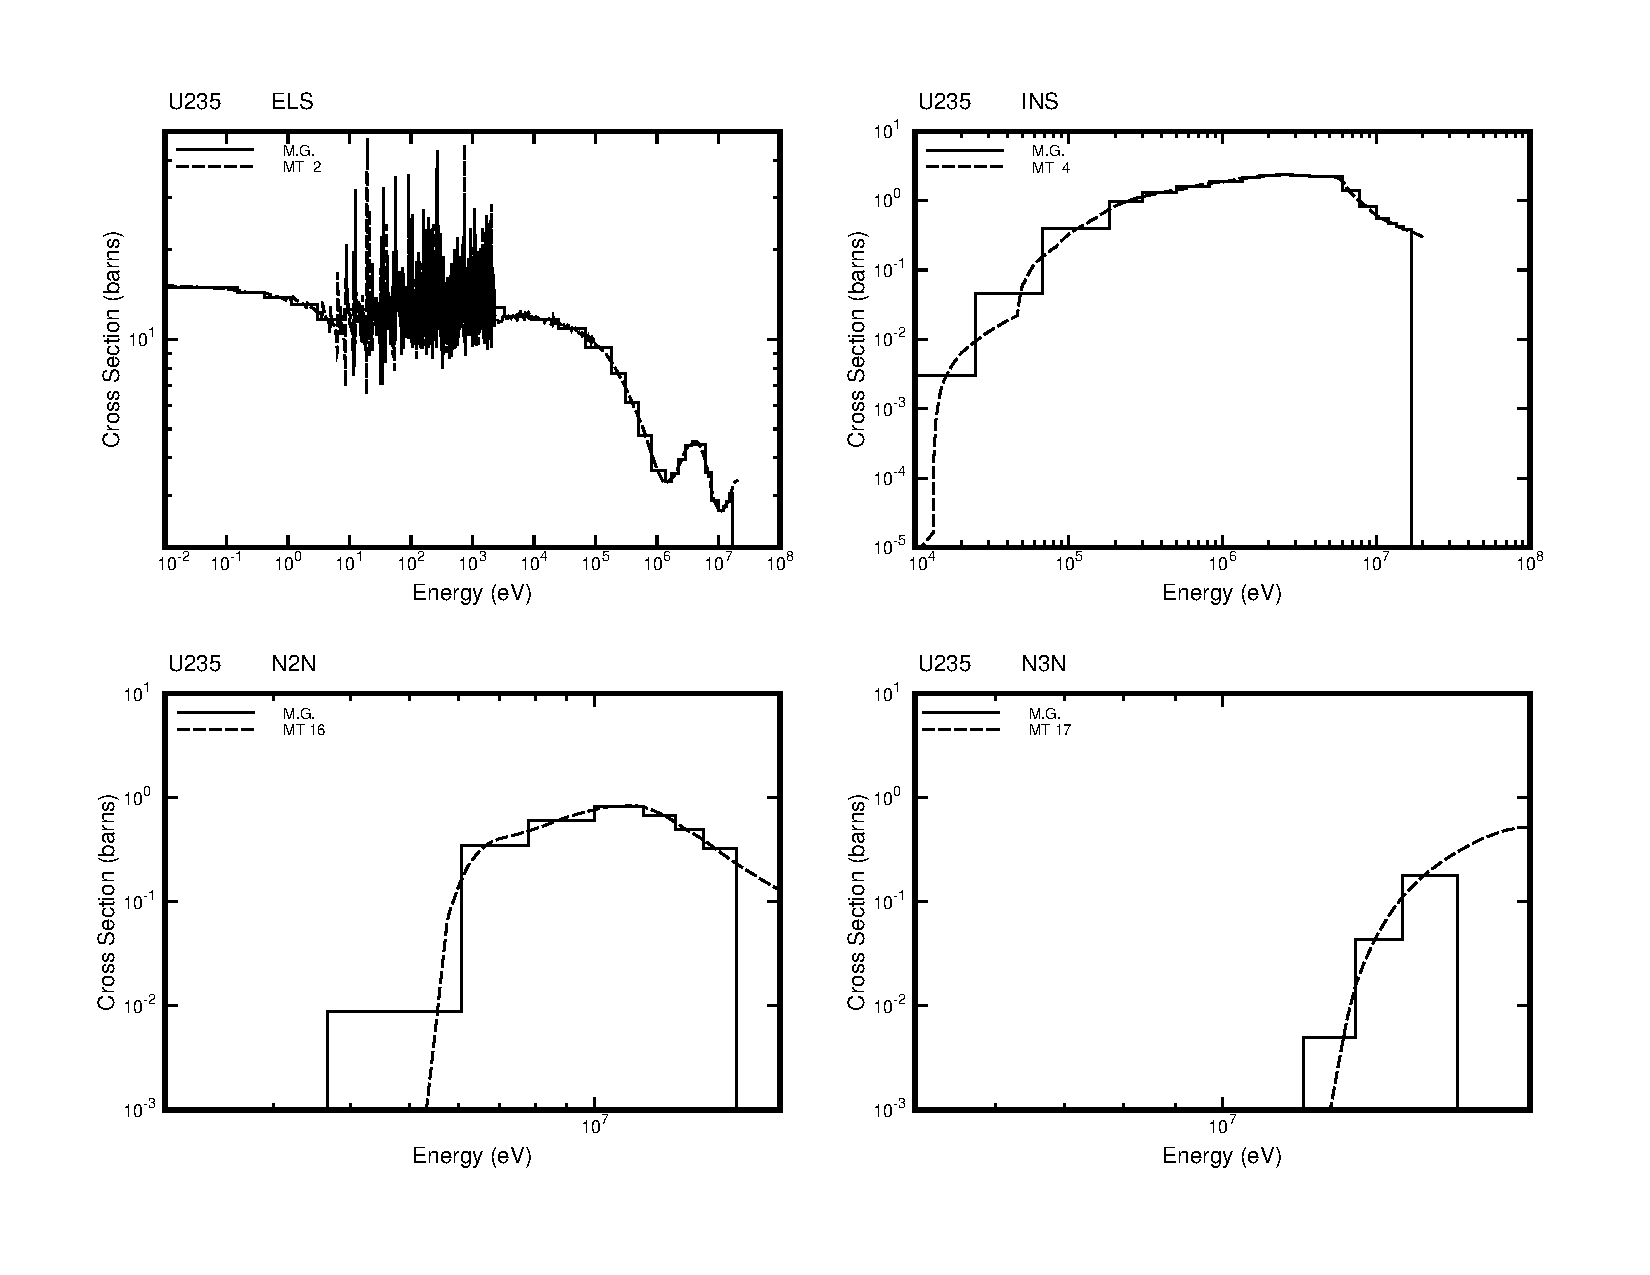
\includegraphics[keepaspectratio, height=3.2in, angle=0]{figs/dtfr5ack}
\caption[DTFR plot example, multiple plots per frame]{An example of DTFR
 plotting using \cword{ifilm=2} for ENDF/B-VI $^{235}$U for some of the
 standard edits with \cword{iedit=1}.}
\label{four}
\end{figure}

\subsection{User Input}
\label{ssDTFR_inp}

The following user input specifications were copied from the
comment cards at the beginning of the DTFR module source code.
\index{DTFR!DTFR input}
\index{input!DTFR}

\small
\begin{ccode}

   !---input specifications (free format)---------------------------
   !
   ! card 1       units
   !    nin       input unit with data from groupr (binary).
   !    nout      output unit containing dtf tables (coded).
   !              (default=0=none)
   !    npend     input unit with pendf tape for point plots.
   !              (default=0=none)
   !    nplot     output plot info for plotr module
   !              (default=0=none)
   ! card 2       options
   !    iprint    print control (0 minimum, 1 maximum)
   !    ifilm     film control (0/1/2=no/yes with 1 plot per frame/
   !              yes with 4 plots per frame (default=0)
   !    iedit     edit control (0/1=in table/separate) (default=0)
   !
   !       cards 3 through 5 only for iedit=0
   !
   ! card 3       neutron tables
   !    nlmax     number of neutron tables desired.
   !    ng        number of neutron groups
   !    iptotl    position of total cross section
   !    ipingp    position of in-group scattering cross section.
   !    itabl     neutron table length desired.
   !    ned       number of entries in edit table (default=0).
   !    ntherm    number of thermal groups (default=0).
   !  card 3a only for ntherm ne 0
   ! card 3a      thermal incoherent and coherent mts
   !    mti       mt for thermal incoherent data
   !    mtc       mt for thermal coherent data (default=0)
   !    nlc       no. coherent legendre orders (default=0)
   ! card 4       edit names
   !       six character hollerith names for edits for as many
   !       cards as needed.  there will be iptotl-3 names read.
   !       each name is delimited with '.
   ! card 5       edit specifications
   !       ned triplets of numbers on as many cards as needed.
   !       positions can appear more than once.
   !       reaction types can appear more than once.
   !    jpos      position of edit quantity.
   !    mt        endf reaction number.
   !    mult      multiplicity to be used when adding this mt.
   !
   !       card 6 for iedit=1
   !
   ! card 6       claw-format tables
   !    nlmax     number of neutron tables (def=5)
   !    ng        number of neutron groups (def=30)
   !              (number of thermal groups is zero)
   !
   ! card 7       gamma ray tables
   !    nptabl    number of gamma tables desired (default=0)
   !    ngp       number of gamma groups (default=0)
   ! card 8       material description
   !       one card for each table set desired.
   !       empty card (/) terminates execution of dtfr.
   !    hisnam    6-character isotope name
   !    mat       material number as in endf (default=0)
   !    jsigz     index number of sigma-zero desired (default=1)
   !    dtemp     temperature desired (default=300)
   !
   !-------------------------------------------------------------------

\end{ccode}
\normalsize

As usual, card 1 is used to assign the input and output units
for the module.  \cword{nin} must be an output tape from
\hyperlink{sGROUPRhy}{GROUPR},
and it can be in either binary or coded mode.  The output
file \cword{nout} must be in coded mode.  It will contain the
DTF-format card images.  File \cword{npend} should be the same PENDF
tape that was used in \hyperlink{sGROUPRhy}{GROUPR}
when \cword{nin} was made.  It is
only needed if plots are requested.  The \cword{nplot} file will
contain the input lines that
\hyperlink{sVIEWRhy}{VIEWR} will use to prepare the Postscript
plots of the DTFR resilts.  Card 2 starts out with the print flag
\cword{iprint}, which is usually set to 1.  The parameter \cword{ifilm}
can be used to suppress plotting, or to request plots with either
1 or 4 graphs per frame.  Examples of the DTFR plotting capability
were given above.  The value of \cword{iprint} is used to control the
output format.  If it is equal to zero, a conventional DTF-type table
is produced.  If any edits were requested, they are given in the
table using the first few positions in the table.  The separate-edits
option is used to produce cross sections in the ``CLAW'' format.
In this format, the edits are extracted from the table and
written out separately with identification information appended
to the right side of each card image.  The scattering tables
have only the standard 3 edits, and they also have standard
identification fields added to the right side of each card.
Examples of both styles were given above.

Cards 3 through 5 are used for \cword{iedit=0} only.  The first
parameter is \cword{ilmax}.  It is the number of Legendre tables
desired; that is, it would be 4 for a P$_3$ set.  The number of
groups \cword{ng} must agree with the number on the input tape
from \hyperlink{sGROUPRhy}{GROUPR}.  The value of
\cword{iptotl} is used to determine both
the position of the total cross section in the table and the number
of special edit positions at the front of the table (\cword{iptotl-3},
which can be zero).  Note that \cword{ned} is not the number of
edit positions; it is the number of edit specification triplets
to be read.  Therefore, \cword{ned}$\ge$\cword{iptotl-3}.
Also \cword{ipingp}=\cword{iptotl}+1 if there is no upscatter, and
\cword{ipingp}=\cword{iptotl}+\cword{nup}+1 when the total number of upscatter
groups is \cword{nup}.  (The parameter \cword{nup} is not actually given
in the input; it is always equal to \cword{ipingp-iptotl-1}.)
The length of a full table is given by

\begin{center}
\begin{tabular}{cl}
  & \cword{iptotl-3}  \\
+ &  \cword{3}   \\
+ & \cword{nup} \\
+ & \cword{ng} \\ \hline
  & \cword{itable}
\end{tabular}
\end{center}

\noindent
However, smaller table lengths can be requested; truncation
will be performed in a way that preserves the production cross
sections.  The parameter \cword{ntherm} can be set to zero if
no thermal upscatter cross sections are desired.  If nonzero,
it refers to the number of incident thermal groups, and it is
used to define the breakpoint between the thermal and epithermal
treatments.  It is not necessarily equal to \cword{nup}.

Card 3a is only given if \cword{ntherm>0}.  It gives the \cword{mt}
numbers for the thermal incoherent and coherent cross sections to
be extracted from the GENDF tape.  Examples might include
221 and zero for free-gas scattering, or 229 and 230 for graphite.
\cword{NLC} can be used to truncate the anisotropy of the coherent
term, if desired.  For thermal cases, DTFR subtracts the
static elastic scattering from both the total and absorption
positions for the lowest \cword{ntherm} groups, and then it adds
in the cross sections corresponding to \cword{mti} and \cword{mtc}
for these thermal groups.  When reading through the matrices, it
omits all the contributions from the static elastic matrix for
the thermal groups, and adds in the \cword{mti} and \cword{mtc}
contributions for these groups instead.

Card 4 gives Hollerith names for the edit cross sections.  These
\cword{ned} names will appear on the output listing, but they
are not passed on to the output file.

Card 5 specifies the
contents of each of the special edit fields.  Note that each
edit can be any linear combination of the cross sections on the
input GENDF tape.  This feature can be used to produce complex
edits like gas production. An example follows:

\small
\begin{ccode}

  1.   ...
  2.   n.he4 kerma fiss
  3.   1 107/
  4.   1 91 3/
  5.   2 301/
  6.   3 444/
  7.   ....

\end{ccode}
\normalsize

\begin{figure}[b]\centering
\includegraphics[keepaspectratio, height=4.0in, angle=270]{figs/dtfr6ack}
\caption[DTFR plot example, compound edit]{An example of a DTFR edit plot
   showing multiple pointwise curves that are the components
   of a compound edit.  This graph is for ENDF/B-IV $^{12}$C
   helium production.  The histogram gives the sum of the
   (n,$\alpha$) cross section and three times the
   (n,n$'$)3$\alpha$ cross section.}
\label{mult}
\end{figure}

\noindent
The line numbers are not part of the input.  Line 1 represents all
the input cards before card 4, and line 7 represents all the
cards after card 5.  This input is for ENDF/B-IV $^{12}$C.
Lines 3 and 4 construct a helium-production cross section as
the sum of (n,$\alpha$) and three times (n,n$'$)3$\alpha$.
Lines 5 and 6 assign two more edit positions for heating and
damage, respectively.  The MT numbers used for the \cword{mt}
field on card 5 are usually just the ENDF MT numbers for the
reaction.  However, there are special values available
to request the weighting flux, the steady-state and delayed
components of the fission neutron spectrum, or the delayed
fission neutron yield.  Remember that the steady-state fission
neutron production cross section will be found in position
\cword{iptotl-1} of the transport table.

When a multigroup edit is a combination of several cross sections
as in this example, the plot of the edit includes the pointwise
cross sections for all of the component reactions.  Figure~\ref{mult}
illustrates this for the $^{12}$C helium-production reaction.
Another useful technique is to build up a compound edit out of two
reactions using a multiplicity of zero for the second reaction.
This causes the second reaction to be plotted but not included in
the edit cross section.  This method can be used to compare the
energy-balance (\cword{mt}=301) and kinematic (\cword{mt}=443) versions of the
KERMA factor.  The appropriate input lines are

\small
\begin{ccode}

       ...
       heat/
       1 301 1 1 443 0/
       ...

\end{ccode}
\normalsize

\noindent
Note that this method is used in the predefined edits associated with
\cword{iedit=1} (see Table~\ref{predef}).

Card 6 is used instead if \cword{iedit=1}.  As described
above, the list of special edit cross sections is fixed for
the CLAW format.  Therefore, it is only necessary to give
\cword{nlmax} and \cword{ng}.  The number of thermal groups
is automatically set to zero.

The next card read for either choice of output format is
card 6, which controls the generation of a photon production
matrix.  The number of photon production tables is usually
zero (none), or one.  Only a few materials in the ENDF/B
libraries have anisotropic photon production data.  Of course,
\cword{ngp} must agree with the photon group structure used
in \hyperlink{sGROUPRhy}{GROUPR}.

The input deck ends with a material description card for
each material to be processed.  These materials must all be
on the input GENDF tape. (Multi-MAT GENDF tapes can be prepared
using \hyperlink{sMODERhy}{MODER} from single-material
\hyperlink{sGROUPRhy}{GROUPR} output files, but since
it is easy to combine materials at the DTF-format stage, DTFR
is usually run for one MAT at a time.) The Hollerith
material names given will appear in the comment cards before
tables and in the special labels added to the right-hand edge
of each card.  The material numbers \cword{mat} are the same ENDF
MAT numbers used when preparing the multigroup cross sections.
DTFR has only a limited capability for handling self-shielded
cross sections.  The user can specify that a given set of tables
be prepared using one particular temperature \cword{dtemp}
and one particular background cross section, the \cword{jsigz}$^{\rm{th}}$
value in the set.

\subsection{Coding Details}
\label{ssDTFR_details}

The main entry point for DTFR is \cword{dtfr}\index{dtfr@{\ty dtfr}}
from module \cword{dtfm}\index{modules!dtfm@{\ty dtfm}}, which
starts by calling \cword{ruin} to read the user's input.  Note that
the special set of edits used when \cword{iedit=1} is specified
using parameter arrays in \cword{ruin} (see \cword{kmted},
\cword{kjped}, \cword{kmultd}, and \cword{kmtid}).  The next
steps are to open a scratch file \cword{nscr} and to initialize
the plotting output.

The main loop over materials, dilution values, and temperatures
goes through statement number 105.  This is where input card number
8 is read (see input instructions) to identify the material to
be processed.  The input GENDF tape is then rewound,  and \cword{nin}
is searched for the material and temperature.  If a PENDF input tape
has been mounted, the corresponding material and temperature are
located on \cword{npend}.  Note that the materials in the input
file do not have to be in the same order as the materials on either
\cword{nin} or \cword{npend}.  If a requested material or temperature
is not found, a fatal error message is issued.

When the input files have been properly positioned, \cword{dtfr}
checks to see if there is enough storage for the tables.  The
limit \cword{nwsmax=500000} is large enough for any reasonable
multigroup set.  If larger sets are desired, increase the value of
this variable which will
automatically increase the dimension of the global array \cword{sig(nwsmax)}.
The loop over reactions and groups in a reaction goes through
statement number 150.  Once the cross sections have been read
off the input tape, the code branches to different sections to
process different kinds of data.  The first of these processes
the File 3 neutron cross sections.  Note that the total cross
section is stored in both \cword{iptotl} and \cword{iptotl-2}.  In
addition, the \hyperlink{sGROUPRhy}{GROUPR}
weighting flux can be extracted from the
section \cword{mf}=3, \cword{mt}=1 and stored into a special edit
requested using
\cword{mt}=300.  Special edit cross sections are weighted with the
specified multiplicities and summed into the specified edit
positions in the ``\cword{do ied=1,ned}'' loop.  Thermal
corrections to static scattering are made at statement number 260.
The method used is to subtract \cword{mt}=2 and add \cword{mti}
and \cword{mtc} to both the total and absorption positions.

The block of coding starting with statement number 300 is used to
accumulate the total scattering matrix.  Most numbers are simply
added into the correct position in the transport table.  The
operation specified by Eq.~\ref{abs} is performed by subtracting
all matrix elements from the absorption position.  In addition,
in the thermal range, the \cword{mti} and  \cword{mtc} data are used instead
of the \cword{mt}=2 data.

The prompt part of fission is handled starting at statement number
340.  Note that a check is made to see if MT=18 was already processed
if \cword{mt}=19 is found.  This results in a fatal error, so the user must
be careful to process only one of these representations in
\hyperlink{sGROUPRhy}{GROUPR}.
The special cases \cword{ig=0} and \cword{ig2lo=0} flag the
presence of the low-energy constant spectrum or production cross
section, respectively.  Delayed fission contributions are handled
by the next block of coding.  The method used for combining
the fission matrix, the constant-spectrum part, and the delayed
parts are defined by Eqs.~\ref{ssnu} and \ref{sschi}.  The
normalization parameter needed to fix up $\chi$ is accumulated in
the variable \cword{cnorm}.

The photon-production matrix is accumulated starting at statement
number 600.  It is a very simple process of adding all the
partial matrices with \cword{mf}=16 on the input GENDF file.
When all the reactions and groups for this material and
temperature have been processed, \cword{dtfr} calls the
subroutine \cword{dtfout}\index{dtfout@{\ty dtfout}} to prepare
the tables and plots, and then it loops back to statement number 105
for the next requested material.  After all the materials, temperatures,
and background cross sections have been written out, the plotting
system is terminated (see below), files are closed, a final
message is printed, and control is returned to \cword{njoy}.

Subroutine \cword{dtfout}\index{dtfout@{\ty dtfout}}
controls the preparation of the output DTF tables on \cword{nout},
the printing of the tables on the user's output device, and
the preparation of plots.  This is a simple routine with separate
paths for in-table edits and separate edits.  Plotting is handled
using different subroutines for the edits, the neutron table, and
the photon-production table.

Subroutine \cword{ploted}\index{ploted@{\ty ploted}} is used to
prepare plots of all the special and standard edit positions,
including overlay plots of PENDF cross sections if \cword{npend}
is available.  Subroutine \cword{histod}\index{histod@{\ty histod}}
is used to convert the multigroup values into a pointwise
cross section with steps at each of the group boundary energies;
that is, into histogram form.  Subroutine
\cword{dpend}\index{dpend@{\ty depend}} prepares the PENDF part
of the plot by thinning the original PENDF grid down to a new grid with
$x$ spacing something like the resolution of a typical screen.
In addition, it ``thickens'' reactions, if necessary, so that
there are enough points to properly follow the curve on the
final log-log plot.  Both the histogram and PENDF data arrays
are written on the the \cword{nplot} unit as simple text
commands in \hyperlink{sVIEWRhy}{VIEWR}\index{VIEWR} format.

Subroutine \cword{plotnn}\index{plotnn@{\ty plotnn}} is used to
plot an isometric view of the neutron table.  This is done by
removing the edits from the table and then writing lines to
\cword{nplot}.  Note that the energies corresponding to the groups
are used in the \hyperlink{sVIEWRhy}{VIEWR} commands, thus producing
more realistic pictures
than the older DTFR methods was able to make.  A similar process is
performed in \cword{plotnp}\index{plotp@{\ty plotp}} for the
photon-production matrix.


\subsection{Error Messages}
\label{ssDTFR_msg}

\begin{description}
\begin{singlespace}

\item[\cword{error in dtfr***number of neutron groups disagrees with...}] ~\par
   The value of \cword{ng} in the input must be consistent with
   the number of groups on the input GENDF tape.  Check the input, and
   check whether the correct tape was mounted.

\item[\cword{error in dtfr***number of gamma groups disagrees with...}] ~\par
   Same as above, except check the number of gamma groups \cword{ngp}.

\item[\cword{error in dtfr***desired temperature not on pendf}] ~\par
   Code is unable to find \cword{mat} and \cword{dtemp} on the
   input PENDF tape \cword{npend}.  Check the input information
   and check whether the correct PENDF tape was mounted.

\item[\cword{error in dtfr***not enough storage for table}] ~\par
   There is not enough space in the \cword{sig} array to construct a table
   with so many positions and groups. See the global parameter
   \cword{nwsmax=500000}.

\item[\cword{error in dtfr***not enough storage for record}] ~\par
   There is not enough space in the \cword{a} array to read in the
   data on the GENDF tape. See the global parameter \cword{nwamax=40000}.

\item[\cword{error in dtfr***mt18 already processed//mt19 not allowed}] ~\par
   Make sure that \hyperlink{sGROUPRhy}{GROUPR} processes the fission
   matrix using either \cword{mt}=18 only, or \cword{mt}=19, 20, 21,
   and 38, but not both.

\item[\cword{error in dtfr***delayed nubar required to add delayed ....}] ~\par
   The delayed neutron yield must have been processed in
   \hyperlink{sGROUPRhy}{GROUPR}
   (\cword{mfd}=3, \cword{mtd}=455), or DTFR will be unable to construct the
   steady-state fission vectors.

\item[\cword{error in ruin***iping.le.iptotl}] ~\par
   The ingroup position \cword{iping} is normally \cword{iptotl}+1,
   and it will be larger still if thermal upscatter is to be included.
   Check input card number 3.

\item[\cword{error in ruin***not enough storage for edits}] ~\par
   See the global parameter \cword{nedmax=50}.

\item[\cword{error in dpend***npts exceeds ndim}] ~\par
   The thinning/thickening process has produced too many points
   for the arrays \cword{x} and \cword{y}.  These are global
   arrays dimensioned at by the global parameter \cword{ndim=7000}.

\end{singlespace}
\end{description}

\cleardoublepage


\section{CCCCR}
\label{sCCCCR}

\hypertarget{sCCCCRhy}{This}
module is used to produce the standard CCCC interface files
ISOTXS, BRKOXS, and DLAYXS from
\hyperlink{sGROUPRhy}{GROUPR} output.

This chapter describes the CCCCR module in NJOY2016.0.

\subsection{Introduction}
\label{ssCCCCR_intro}

The CCCC interface files (commonly pronounced ``four cees'') were
developed by the Committee for Computer Code Coordination for the
US Fast Breeder Reactor Program.\index{CCCC interface files}
\index{Fast Breeder Reactor Program}  When
the members of this committee started work in 1970,
they noted that because of the large variety of
computers and computer systems, computer codes developed at one
laboratory were often incompatible with computers at other
laboratories.  Major rewrites of codes or wasteful duplicate efforts
were common.  They hoped to create a system that would allow different
laboratories to create codes that could be moved to other sites more
easily.  Moreover, they hoped that the codes developed at different
laboratories could easily work together, thereby achieving larger and
more capable calculational systems than any one laboratory could hope to
develop by itself.

Much of the following discussion was developed long ago, and so some
of the code examples conform to FORTRAN-77.  We assume the reader can
easily convert this into modern Fortran.

They approached this problem in two ways.  First, they tried to establish
general programming standards that would make computer codes more
portable.  And second, they tried to establish standard interface files
for reactor physics codes that would make it easier for computer codes to
communicate with each other.  The results of this work appeared in fullest
form as the CCCC-III and CCCC-IV standards\cite{CCCC3,CCCC4}.
\index{CCCC format!CCCC-III}
\index{CCCC format!CCCC-IV}

The MINX\index{MINX} code\cite{MINX}, which was the predecessor of NJOY,
was able to produce libraries \cite{LIBIV}\index{LIB-IV} that used
the CCCC-III interface formats.  The LINX\index{LINX} and
BINX\index{BINX} library management codes\cite{LINXBINX} and the
CINX\index{CINX} group collapse code\cite{CINX} were also released
during this period.  Major codes that used data in CCCC-format
included SPHINX\cite{SPHINX}\index{SPHINX} from
Westinghouse\index{Westinghouse}, TDOWN\cite{TDOWN}\index{TDOWN}
from General Electric\index{General Electric},
DIF3D\cite{DIF3D}\index{DIF3D} from Argonne National Laboratory,
\index{Argonne National Laboratory!ANL} and ONEDANT\cite{ONEDANT}\index{ONEDANT}
from LANL\index{Los Alamos National Laboratory!LANL}.  It was indeed found that
codes could be moved more easily than before.  Analysts could use
ONEDANT and DIF3D on similar problems; they could even use one code to
generate utility files (for example, mixture and geometry files) that
would work with the other code!  When NJOY was developed, it first
produced version III formats and was later upgraded to the CCCC-IV
standard.

With the demise of the breeder reactor program, development of the CCCC
system has stopped.  However, many good programs are still available
that make use of CCCC files and programming standards.  The LANL
DANDE system\cite{DANDE} was an example of how the use of standard
interface files can be used to couple several reactor physics programs
together into an easy-to-use and powerful product.  In areas where the
CCCC standards were not very successful, such as gamma ray cross
sections and cross sections for the fusion energy range,
the MATXS format is available as an alternative.  This generalized
material cross section library format uses CCCC-type techniques.
The modern S$_{\rm N}$ code PARTISN\cite{PARTISN} makes very heavy
use of both standard and non-standard CCCC files  Thus, the CCCC
spirit is not dead.
\index{DANDE}
\index{MATXS format}

\subsection{CCCC Procedures and Programming Standards}
\label{ssCCCCR_Proc}

Although the CCCC programming standards went so far as to give advice on
program structure, documentation, and good coding practice, their main
purpose was to make it easier to move computer codes from one machine
to another.  The main problems in those days were the slightly different
implementations of input/output on CDC and IBM machines, the different
word size on CDC and IBM machines, and the relatively small size of the
main memory on the CDC 7600.  The last of these problems was attacked by
limiting the maximum memory requirements for CCCC-compliant codes.  This
problem has disappeared for modern computers.

The word-size problem has three components.  First, it is often
necessary to change the statements that allocate space for variables
and arrays [for example, ``\cword{DIMENSION A(10)}'' might have to be
changed to ``\cword{REAL*8 A(10)}'' when moving from a long-word
machine (CDC, Cray) to a short-word machine (IBM, VAX, Sun)].  Second,
the names of functions that work with double-precision variables
normally must be changed (for example, \cword{ALOG10} to \cword{DLOG10}).
And third, the word boundaries of double-precision variables must be
properly aligned in common blocks and equivalenced arrays.  The standard
CCCC method for handling name changes has been based on using standard
control cards.  As an example, a code for a long-word machine might
contain the following code fragment:

\newpage
\small
\begin{ccode}

CSW
C     REAL*8 HA(10)
CSW
CLW
      INTEGER HA(10)
CLW

\end{ccode}
\normalsize

The variable \cword{HA} is intended to hold 10 words of Hollerith
information using the standard CCCC 6-character word length.  Such a
variable must be declared as double precision on short-word machines,
which typically allow four Hollerith characters per word.  To change
this code to its short-word version, a special utility code reads
through each line removing the comment ``C'' from lines bracketed by
the ``SW'' comments and inserting a ``C'' in column 1 for all lines
bracketed by ``LW'' comments.  Early versions of NJOY used this
scheme; later versions used UPD\cite{UPD} conditional
\index{UPD}
statements instead.  For example, the source file contained

\small
\begin{ccode}

*IF SW
      REAL*8 HA(10)
*ELSE
      INTEGER HA(10)
*ENDIF

\end{ccode}
\normalsize

\noindent
and the compile file produced by UPD had only one of the two
alternatives activated, depending on whether \cword{SW} has been
set or not.  NJOY2016 uses built-in features of Fortran-90 to
handle this problem.  The \cword{locale} module defines a
special "kind" for the Hollerith data that is packed into
CCCC records.

The word-alignment problem requires that some care be used in
allocating arrays and common blocks.  For example,

\small
\begin{ccode}

REAL*8 HA
COMMON/BAD/IA(3),HA(10)

\end{ccode}
\normalsize

\noindent
should be avoided; it would be OK with \cword{IA(4)}.  Most CCCC records
contain mixtures of Hollerith, floating-point, and integer variables.
The desired data is normally extracted by making use of equivalenced
arrays.  For example, a code could contain the following declarations:

\small
\begin{ccode}

REAL*8 HA(10)
DIMENSION A(20),IA(20)
EQUIVALENCE (HA(1),A(1)),(IA(1),A(1))

\end{ccode}
\normalsize

\noindent
Assume that a record containing 2 Hollerith variables (which require
two single-precision variables each), 2 floating-point numbers (at
single precision), and 2 integers has been read into array \cword{A}.
How do you extract the first of the integers? The solution depends on
defining a CCCC-standard quantity called \cword{mult},
\index{mult@{\ty mult}}
which is 1 for long-word machines and 2 for short-word machines.  Now,
the desired value can be obtained with an expression of the form

\small
\begin{ccode}

I1=IA(2*MULT+3)

\end{ccode}
\normalsize

\noindent
The second Hollerith variable would be extracted using the simple
expression

\small
\begin{ccode}

H2=HA(2)

\end{ccode}
\normalsize

\noindent
Changing the value of \cword{mult} when transporting a code to a
different machine is easily handled using control-card brackets or UPD
conditionals as described above.

In NJOY2012 and later, common blocks are no longer used, but equivalencing
is still used to pack Hollerith (or character), integer, and real data
into the CCCC records.  While such coding techniques may bring tears to
the eyes of modern programmers, it remains a valid coding mechanism and
we continue to exploit this capability.

The remaining feature of the CCCC programming standards that is used
in codes like PARTISN is the concept of standardized input/output subroutines.
The CCCC interface files are sequential binary files (binary for
efficiency and sequential for simplicity).  The interface formats are
arranged so that the length of any record can be calculated using
parameters already read from previous records.  It is convenient to
insulate CCCC input/output from system variations by defining two
standard routines:
\index{REED@{\ty REED}}
\index{RITE@{\ty RITE}}

\begin{description}
\begin{singlespace}

\item[\cword{REED(NREF,IREC,ARRAY,NWDS,MODE)}] ~\par
  Read record \cword{IREC} from unit \cword{NREF} into
  \cword{ARRAY}.  The record has length \cword{NWDS}
  in single-precision words.  The \cword{MODE} parameter
  is used to control I/O buffering, and it is not used
  in NJOY. Records can be read out of sequence; the
  routine does any record skipping (forward or backward)
  needed to arrive at record number \cword{IREC}.
\item[\cword{RITE(NREF,IREC,ARRAY,NWDS,MODE)}] ~\par
  Write record \cword{IREC} onto unit \cword{NREF} using
  the data in \cword{ARRAY}.  The first \cword{NWDS}
  single-precision words will be written.  The \cword{MODE}
  parameter is ignored.  The records \cword{NREF} must be
  written in sequence.  The unit will be rewound if
  \cword{IREC=1}.

\end{singlespace}
\end{description}

\noindent
When transporting a code between different computer systems,
it is only necessary to have (or prepare) operational versions
of \cword{REED} and \cword{RITE} for the target machine.

In the conversion to Fortran-90 style, we tried to avoid all these
tricks.  The reading and writing of CCCC records was coded in
directly to avoid word-length problems (no more REED or RITE).  All
internal variable and data read from the GENDF file use 8-byte words.
It is only at the last stage when the data are stored into the CCCC
records that the 8-byte data are converted to 4-byte words.  Thus,
\cword{mult} is always equal to 2.  In general, the accuracy
obtained with 4-byte words is sufficient for multigroup data.

\subsection{The Standard Interface Files}
\label{ssCCCCR_Interface}

The CCCCR module produces data libraries that use three of the CCCC-IV
standard interface files, namely:
\index{ISOTXS}
\index{BRKOXS}
\index{DLAYXS}

\begin{description}
\begin{singlespace}

\item[ISOTXS] for nuclide (isotope)-ordered multigroup neutron
  cross sections including cross section versus energy functions
  for the principal cross sections, group-to-group scattering
  matrices, and fission neutron production and spectra tables;
\item[BRKOXS] for Bondarenko-type self-shielding factors versus
  energy group, temperature, and background cross section for
  the reactions with major resonance contributions; and
\item[DLAYXS] for delayed-neutron precursor yields, emission
  spectra, and decay constants for the major fissionable
  isotopes.

\end{singlespace}
\end{description}

\noindent
The format of each of these files, the definition of the types of data
included, and the uses and weaknesses of these three standard file
formats are discussed in the following three sections.

As mentioned in the preceding section, the normal form of the CCCC files
is binary and sequential.  CCCCR writes its output in this binary mode.
Of course, coded versions (ASCII for modern systems) are needed to move
library files between different machines, and the formats used for the
coded versions are given in the file descriptions below.  A separate
program, BINX\cite{LINXBINX}, is used to convert back and forth between
coded and binary modes.  BINX can also be used to prepare an
interpreted listing of a library.  CCCCR can prepare an entire
multimaterial library in one run if a multimaterial GENDF file is
available.  It can also be used to prepare an interface file containing
only one material.  These one-material files can be merged into
multimaterial libraries using the LINX code\cite{LINXBINX}.

\subsection{ISOTXS}
\label{ssCCCCR_ISOTXS}

The format for the ISOTXS\index{ISOTXS} material (isotope)-ordered
cross section file is given below.  This computer-text format is
standard for the CCCC interface files.  Of course, if these lines
were to be inserted into a modern Fortran (say .f90 or later)
code, the initial "C" will have to be changed to ``!".

\small
\begin{ccode}

C***********************************************************************
C                       REVISED 11/30/76                               -
C                                                                      -
CF          ISOTXS-IV                                                  -
CE          MICROSCOPIC GROUP NEUTRON CROSS SECTIONS                   -
C                                                                      -
CN                      THIS FILE PROVIDES A BASIC BROAD GROUP         -
CN                      LIBRARY, ORDERED BY ISOTOPE                    -
CN                      FORMATS GIVEN ARE FOR FILE EXCHANGE PURPOSES   -
CN                      ONLY.                                          -
C                                                                      -
C***********************************************************************

C-----------------------------------------------------------------------
CS          FILE STRUCTURE                                             -
CS                                                                     -
CS             RECORD TYPE                        PRESENT IF           -
CS             ===============================    ===============      -
CS             FILE IDENTIFICATION                ALWAYS               -
CS             FILE CONTROL                       ALWAYS               -
CS             FILE DATA                          ALWAYS               -
CS             FILE-WIDE CHI DATA                 ICHIST.GT.1          -
CS   **************(REPEAT FOR ALL ISOTOPES)                           -
CS   *         ISOTOPE CONTROL AND GROUP                               -
CS   *                        INDEPENDENT DATA    ALWAYS               -
CS   *         PRINCIPAL CROSS SECTIONS           ALWAYS               -
CS   *         ISOTOPE CHI DATA                   ICHI.GT.1            -
CS   *  **********(REPEAT TO NSCMAX SCATTERING BLOCKS)                 -
CS   *  *  *******(REPEAT FROM 1 TO NSBLOK)                            -
CS   *  *  *   SCATTERING SUB-BLOCK               LORD(N).GT.0         -
CS   *************                                                     -
C                                                                      -
C-----------------------------------------------------------------------

C-----------------------------------------------------------------------
CR          FILE IDENTIFICATION                                        -
C                                                                      -
CL    HNAME,(HUSE(I),I=1,2),IVERS                                      -
C                                                                      -
CW    1+3*MULT=NUMBER OF WORDS                                         -
C                                                                      -
CB    FORMAT(11H 0V ISOTXS  ,1H*,2A6,1H*,I6)                           -
C                                                                      -
CD    HNAME       HOLLERITH FILE NAME - ISOTXS -                       -
CD    HUSE(I)     HOLLERITH USER IDENTIFICATION (A6)                   -
CD    IVERS       FILE VERSION NUMBER                                  -
CD    MULT        DOUBLE PRECISION PARAMETER                           -
CD                    1- A6 WORD IS SINGLE WORD                        -
CD                    2- A6 WORD IS DOUBLE PRECISION WORD              -
C                                                                      -
C-----------------------------------------------------------------------

C-----------------------------------------------------------------------
CR          FILE CONTROL   (1D RECORD)                                 -
C                                                                      -
CL    NGROUP,NISO,MAXUP,MAXDN,MAXORD,ICHIST,NSCMAX,NSBLOK              -
C                                                                      -
CW    8=NUMBER OF WORDS                                                -
C                                                                      -
CB    FORMAT(4H 1D ,8I6)                                               -
C                                                                      -
CD    NGROUP        NUMBER OF ENERGY GROUPS IN FILE                    -
CD    NISO          NUMBER OF ISOTOPES IN FILE                         -
CD    MAXUP         MAXIMUM NUMBER OF UPSCATTER GROUPS                 -
CD    MAXDN         MAXIMUM NUMBER OF DOWNSCATTER GROUPS               -
CD    MAXORD        MAXIMUM SCATTERING ORDER (MAXIMUM VALUE OF         -
CD                     LEGENDRE EXPANSION INDEX USED IN FILE).         -
CD    ICHIST        FILE-WIDE FISSION SPECTRUM FLAG                    -
CD                     ICHIST.EQ.0,      NO FILE-WIDE SPECTRUM         -
CD                     ICHIST.EQ.1,      FILE-WIDE CHI VECTOR          -
CD                     ICHIST.GT.1,      FILE-WIDE CHI MATRIX          -
CD    NSCMAX        MAXIMUM NUMBER OF BLOCKS OF SCATTERING DATA        -
CD    NSBLOK        SUBBLOCKING CONTROL FOR SCATTER MATRICES. THE      -
CD                     SCATTERING DATA ARE SUBBLOCKED INTO NSBLOK      -
CD                     RECORDS (SUBBLOCKS) PER SCATTERING BLOCK.       -
C                                                                      -
C-----------------------------------------------------------------------

C-----------------------------------------------------------------------
CR          FILE DATA   (2D RECORD)                                    -
C                                                                      -
CL    (HSETID(I),I=1,12),(HISONM(I),I=1,NISO),                         -
CL   1(CHI(J),J=1,NGROUP),(VEL(J),J=1,NGROUP),                         -
CL   2(EMAX(J),J=1,NGROUP),EMIN,(LOCA(I),I=1,NISO)                     -
C                                                                      -
CW    (NISO+12)*MULT+1+NISO                                            -
CW    +NGROUP*(2+ICHIST*(2/ICHIST+1)))=NUMBER OF WORDS                 -
C                                                                      -
CB    FORMAT(4H 2D ,1H*,11A6,1H*/     HSETID,HISONM                    -
CB   11H*,A6,1H*,9(1X,A6)/(10(1X,A6)))                                 -
CB    FORMAT(6E12.5)                  CHI (PRESENT IF ICHIST.EQ.1)     -
CD    FORMAT(6E12.5)                  VEL,EMAX,EMIN                    -
CD    FORMAT(12I6)                    LOCA                             -
C                                                                      -
CD    HSETID(I)     HOLLERITH IDENTIFICATION OF FILE (A6)              -
CD    HISONM(I)     HOLLERITH ISOTOPE LABEL FOR ISOTOPE I (A6)         -
CD    CHI(J)        FILE-WIDE FISSION SPECTRUM(PRESENT IF ICHIST.EQ.1) -
CD    VEL(J)        MEAN NEUTRON VELOCITY IN GROUP J (CM/SEC)          -
CD    EMAX(J)       MAXIMUM ENERGY BOUND OF GROUP J (EV)               -
CD    EMIN          MINIMUM ENERGY BOUND OF SET (EV)                   -
CD    LOCA(I)       NUMBER OF RECORDS TO BE SKIPPED TO READ DATA FOR   -
CD                     ISOTOPE I.  LOCA(1)=0                           -
C                                                                      -
C-----------------------------------------------------------------------

C-----------------------------------------------------------------------
CR          FILE-WIDE CHI DATA   (3D RECORD)                           -
C                                                                      -
CC        PRESENT IF ICHIST.GT.1                                       -
C                                                                      -
CL    ((CHI(K,J),K=1,ICHIST),J=1,NGROUP),(ISSPEC(I),I=1,NGROUP)        -
C                                                                      -
CW    NGROUP*(ICHIST+1)=NUMBER OF WORDS                                -
C                                                                      -
CB    FORMAT(4H 3D ,5E12.5/(6E12.5))   CHI                             -
CB    FORMAT(12I6)                     ISSPEC                          -
C                                                                      -
CD    CHI(K,J)      FRACTION OF NEUTRONS EMITTED INTO GROUP J AS A     -
CD                     RESULT OF FISSION IN ANY GROUP,USING SPECTRUM K -
CD    ISSPEC(I)     ISSPEC(I)=K IMPLIES THAT SPECTRUM K IS USED        -
CD                     TO CALCULATE EMISSION SPECTRUM FROM FISSION     -
CD                     IN GROUP I                                      -
C                                                                      -
C-----------------------------------------------------------------------

C-----------------------------------------------------------------------
CR          ISOTOPE CONTROL AND GROUP INDEPENDENT DATA   (4D RECORD)   -
C                                                                      -
CL    HABSID,HIDENT,HMAT,AMASS,EFISS,ECAPT,TEMP,SIGPOT,ADENS,KBR,ICHI, -
CL   1IFIS,IALF,INP,IN2N,IND,INT,LTOT,LTRN,ISTRPD,                     -
CL   2(IDSCT(N),N=1,NSCMAX),(LORD(N),N=1,NSCMAX),                      -
CL   3((JBAND(J,N),J=1,NGROUP),N=1,NSCMAX),                            -
CL   4((IJJ(J,N),J=1,NGROUP),N=1,NSCMAX)                               -
C                                                                      -
CW    3*MULT+17+NSCMAX*(2*NGROUP+2)=NUMBER OF WORDS                    -
C                                                                      -
CB    FORMAT(4H 4D ,3(1X,A6)/6E12.5/                                   -
CB   1(12I6))                                                          -
C                                                                      -
CD    HABSID        HOLLERITH ABSOLUTE ISOTOPE LABEL - SAME FOR ALL    -
CD                            VERSIONS OF THE SAME ISOTOPE IN FILE (A6)-
CD    HIDENT        IDENTIFIER OF LIBRARY FROM WHICH BASIC DATA        -
CD                            CAME (E.G. ENDF/B) (A6)                  -
CD    HMAT          ISOTOPE IDENTIFICATION (E.G. ENDF/B MAT NO.) (A6)  -
CD    AMASS         GRAM ATOMIC WEIGHT                                 -
CD    EFISS         TOTAL THERMAL ENERGY YIELD/FISSION (W.SEC/FISS)    -
CD    ECAPT         TOTAL THERMAL ENERGY YIELD/CAPTURE (W.SEC/CAPT)    -
CD    TEMP          ISOTOPE TEMPERATURE (DEGREES KELVIN)               -
CD    SIGPOT        AVERAGE EFFECTIVE POTENTIAL SCATTERING IN          -
CD                            RESONANCE RANGE (BARNS/ATOM)             -
CD    ADENS         DENSITY OF ISOTOPE IN MIXTURE IN WHICH ISOTOPE     -
CD                            CROSS SECTIONS WERE GENERATED (A/BARN-CM)-
CD    KBR           ISOTOPE CLASSIFICATION                             -
CD                     0=UNDEFINED                                     -
CD                     1=FISSILE                                       -
CD                     2=FERTILE                                       -
CD                     3=OTHER ACTINIDE                                -
CD                     4=FISSION PRODUCT                               -
CD                     5=STRUCTURE                                     -
CD                     6=COOLANT                                       -
CD                     7=CONTROL                                       -
CD    ICHI          ISOTOPE FISSION SPECTRUM FLAG                      -
CD                      ICHI.EQ.0,     USE FILE-WIDE CHI               -
CD                      ICHI.EQ.1,     ISOTOPE CHI VECTOR              -
CD                      ICHI.GT.1,     ISOTOPE CHI MATRIX              -
CD    IFIS          (N,F) CROSS SECTION FLAG                           -
CD                     IFIS=0, NO FISSION DATA IN PRINCIPAL CROSS      -
CD                                       SECTION RECORD                -
CD                         =1, FISSION DATA PRESENT IN PRINCIPAL       -
CD                                       CROSS SECTION RECORD          -
CD    IALF          (N,ALPHA) CROSS SECTION FLAG                       -
CD                     SAME OPTIONS AS IFIS                            -
CD    INP           (N,P) CROSS SECTION FLAG                           -
CD                     SAME OPTIONS AS IFIS                            -
CD    IN2N          (N,2N) CROSS SECTION FLAG                          -
CD                     SAME OPTIONS AS IFIS                            -
CD    IND           (N,D) CROSS SECTION FLAG                           -
CD                     SAME OPTIONS AS IFIS                            -
CD    INT           (N,T) CROSS SECTION FLAG                           -
CD                     SAME OPTIONS AS IFIS                            -
CD    LTOT          NUMBER OF MOMENTS OF TOTAL CROSS SECTION PROVIDED  -
CD                     IN PRINCIPAL CROSS SECTIONS RECORD              -
CD    LTRN          NUMBER OF MOMENTS OF TRANSPORT CROSS SECTION       -
CD                     PROVIDED IN PRINCIPAL CROSS SECTION RECORD      -
CD    ISTRPD        NUMBER OF COORDINATE DIRECTIONS FOR WHICH          -
CD                     COORDINATE DEPENDENT TRANSPORT CROSS SECTIONS   -
CD                     ARE GIVEN, IS ISTRPD=0, NO COORDINATE DEPENDENT -
CD                     TRANSPORT CROSS SECTIONS ARE GIVEN.             -
CD    IDSCT(N)      SCATTERING MATRIX TYPE IDENTIFICATION FOR          -
CD                     SCATTERING BLOCK N, SIGNIFICANT ONLY IF         -
CD                     LORD(N).GT.0                                    -
CD                     IDSCT(N)=000 + NN, TOTAL SCATTERING, (SUM OF    -
CD                         ELASTIC, INELASTIC, AND N2N SCATTERING      -
CD                         MATRIX TERMS),                              -
CD                             =100 + NN, ELASTIC SCATTERING           -
CD                             =200 + NN, INELASTIC SCATTERING         -
CD                             =300 + NN, (N,2N) SCATTERING,----SEE    -
CD                              NOTE BELOW----                         -
CD                     WHERE NN IS THE LEGENDRE EXPANSION INDEX OF THE -
CD                     FIRST MATRIX IN BLOCK N                         -
CD    LORD(N)       NUMBER OF SCATTERING ORDERS IN BLOCK N.  IF        -
CD                     LORD(N)=0, THIS BLOCK IS NOT PRESENT FOR THIS   -
CD                     ISOTOPE.  IF NN IS THE VALUE TAKEN FROM         -
CD                     IDSCT(N), THEN THE MATRICES IN THIS BLOCK       -
CD                     HAVE LEGENDRE EXPANSION INDICES OF NN,NN+1,     -
CD                     NN+2,...,NN+LORD(N)-1                           -
CD    JBAND(J,N)    NUMBER OF GROUPS THAT SCATTER INTO GROUP J,        -
CD                     INCLUDING SELF-SCATTER, IN SCATTERING BLOCK N.  -
CD                     IF JBAND(J,N)=0, NO SCATTER DATA IS PRESENT IN  -
CD                     BLOCK N                                         -
CD    IJJ(J,N)      POSITION OF IN-GROUP SCATTERING CROSS SECTION IN   -
CD                     SCATTERING DATA FOR GROUP J, SCATTERING BLOCK   -
CD                     N, COUNTED FROM THE FIRST WORD OF GROUP J DATA. -
CD                     IF JBAND(J,N).NE.0 THEN IJJ(J,N) MUST SATISFY   -
CD                     THE RELATION 1.LE.IJJ(J,N).LE.JBAND(J,N)        -
C                                                                      -
CD                  NOTE- FOR N,2N SCATTER, THE MATRIX CONTAINS TERMS  -
CD                     SCAT(J TO G), WHICH ARE EMISSION (PRODUCTION)-  -
CD                     BASED, I.E., ARE DEFINED SUCH THAT MACROSCOPIC  -
CD                     SCAT(J TO G) TIMES THE FLUX IN GROUP J GIVES    -
CD                     THE RATE OF EMISSION (PRODUCTION) OF NEUTRONS   -
CD                     INTO GROUP G.                                   -
C                                                                      -
C-----------------------------------------------------------------------

C-----------------------------------------------------------------------
CR          PRINCIPAL CROSS SECTIONS   (5D RECORD)                     -
C                                                                      -
CL    ((STRPL(J,L),J=1,NGROUP),L=1,LTRN),                              -
CL   1((STOTPL(J,L),J=1,NGROUP),L=1,LTOT),(SNGAM(J),J=1,NGROUP).       -
CL   2(SFIS(J),J=1,NGROUP),(SNUTOT(J),J=1,NGROUP),                     -
CL   3(CHISO(J),J=1,NGROUP),(SNALF(J),J=1,NGROUP),                     -
CL   4(SNP(J),J=1,NGROUP),(SN2N(J),J=1,NGROUP),                        -
CL   5(SND(J),J=1,NGROUP),(SNT(J),J=1,NGROUP),                         -
CL   6((STRPD(J,I),J=1,NGROUP),I=1,ISTRPD)                             -
C                                                                      -
CW   (1+LTRN+LTOT+IALF+INP+IN2N+IND+ISTRPD+2*IFIS+                     -
CW   ICHI*(2/(ICHI+1)))*NGROUP=NUMBER OF WORDS                         -
C                                                                      -
CB   FORMAT(4H 5D ,5E12.5/(6E12.5)) LENGTH OF LIST AS ABOVE            -
C                                                                      -
CD    STRPL(J,L)   PL WEIGHTED TRANSPORT CROSS SECTION                 -
CD                    THE FIRST ELEMENT OF ARRAY STRPL IS THE          -
CD                    CURRENT (P1) WEIGHTED TRANSPORT CROSS SECTION    -
CD                    THE LEGENDRE EXPANSION COEFFICIENT FACTOR (2L+1) -
CD                    IS NOT INCLUDED IN STRPL(J,L).                   -
CD    STOTPL(J,L)  PL WEIGHTED TOTAL CROSS SECTION                     -
CD                    THE FIRST ELEMENT OF ARRAY STOTPL IS THE         -
CD                    FLUX (P0) WEIGHTED TOTAL CROSS SECTION           -
CD                    THE LEGENDRE EXPANSION COEFFICIENT FACTOR (2L+1) -
CD                    IS NOT INCLUDED IN STOTPL(J,L).                  -
CD    SNGAM(J)     (N,GAMMA)                                           -
CD    SFIS(J)      (N,F)        (PRESENT IF IFIS.GT.0)                 -
CD    SNUTOT(J)    TOTAL NEUTRON YIELD/FISSION (PRESENT IF IFIS.GT.0)  -
CD    CHISO(J)I    ISOTOPE CHI  (PRESENT IF ICHI.EQ.1)                 -
CD    SNALF(J)     (N,ALPHA)    (PRESENT IF IALF.GT.0)                 -
CD    SNP(J)       (N,P)        (PRESENT IF INP.GT.0)                  -
CD    SN2N(J)      (N,2N)       (PRESENT IF IN2N.GT.0)  ----SEE        -
CD                    NOTE----                                         -
CD    SND(J)       (N,D)        (PRESENT IF IND.GT.0)                  -
CD    SNT(J)       (N,T)        (PRESENT IF INT.GT.0)                  -
CD    STRPD(J,I)   COORDINATE DIRECTION I TRANSPORT CROSS SECTION      -
CD                              (PRESENT IF ISTRPD.GT.0)               -
C                                                                      -
CN                 NOTE - THE PRINCIPAL N,2N CROSS SECTION SN2N(J)     -
CN                    IS DEFINED AS THE N,2N REACTION CROSS SECTION,   -
CN                    I.E., SUCH THAT MACROSCOPIC SN2N(J) TIMES THE    -
CN                    FLUX IN GROUP J GIVES THE RATE AT WHICH N,2N     -
CN                    REACTIONS OCCUR IN GROUP J.  THUS, FOR N,2N      -
CN                    SCATTERING, SN2N(J) = 0.5*(SUM OF SCAT(J TO G)   -
CN                    SUMMED OVER ALL G).                              -
C                                                                      -
C-----------------------------------------------------------------------

C-----------------------------------------------------------------------
CR          ISOTOPE CHI DATA   (6D RECORD)                             -
C                                                                      -
CC          PRESENT IF ICHI.GT.1                                       -
C                                                                      -
CL    ((CHIISO(K,J),K=1,ICHI),J=1,NGROUP),(ISOPEC(I),I=1,NGROUP)       -
C                                                                      -
CW    NGROUP*(ICHI+1)=NUMBER OF WORDS                                  -
C                                                                      -
CB    FORMAT(4H 6D ,5E12.5/(6E12.5))   CHIISO                          -
CB    FORMAT(12I6)                     ISOPEC                          -
C                                                                      -
CD    CHIISO(K,J)   FRACTION OF NEUTRONS EMITTED INTO GROUP J AS       -
CD                     RESULT OF FISSION IN ANY GROUP,USING SPECTRUM K -
CD    ISOPEC(I)     ISOPEC(I)=K IMPLIES THAT SPECTRUM K IS USED        -
CD                     TO CALCULATE EMISSION SPECTRUM FROM FISSION     -
CD                     IN GROUP I                                      -
C                                                                      -
C-----------------------------------------------------------------------

C-----------------------------------------------------------------------
CR          SCATTERING SUB-BLOCK   (7D RECORD)                         -
C                                                                      -
CC          PRESENT IF LORD(N).GT.0                                    -
C                                                                      -
CL    ((SCAT(K,L),K=1,KMAX),L=1,LORDN)                                 -
C                                                                      -
CC    KMAX=SUM OVER J OF JBAND(J,N) WITHIN THE J-GROUP RANGE OF THIS   -
CC       SUB-BLOCK.  IF M IS THE INDEX OF THE SUB-BLOCK, THE J-GROUP   -
CC       RANGE CONTAINED WITHIN THIS SUB-BLOCK IS                      -
CC       JL=(M-1)*((NGROUP-1)/NSBLOK+1 TO JU=MIN0(NGROUP,JUP),         -
CC       WHERE JUP=M*((NGROUP-1)/NSBLOK+1).                            -
C                                                                      -
CC    LORDN=LORD(N)                                                    -
CC    N IS THE INDEX FOR THE LOOP OVER NSCMAX (SEE FILE STRUCTURE)     -
C                                                                      -
CW    KMAX*LORDN=NUMBER OF WORDS                                       -
C                                                                      -
CB    FORMAT(4H 7D ,5E12.5/(6E12.5))                                   -
C                                                                      -
CD    SCAT(K,L)     SCATTERING MATRIX OF SCATTERING ORDER L, FOR       -
CD                     REACTION TYPE IDENTIFIED BY IDSCT(N) FOR THIS   -
CD                     BLOCK, JBAND(J,N) VALUES FOR SCATTERING INTO    -
CD                     GROUP J ARE STORED AT LOCATIONS K=SUM FROM 1    -
CD                     TO (J-1) OF JBAND(J,N) PLUS 1 TO K-1+JBAND(J,N).-
CD                     THE SUM IS ZERO WHEN J=1, J-TO-J SCATTER IS     -
CD                     THE IJJ(J,N)-TH ENTRY IN THE RANGE JBAND(J,N),  -
CD                     VALUES ARE STORED IN THE ORDER (J+JUP),         -
CD                     (J+JUP-1),...,(J+1),J,(J-1),...,(J-JDN),        -
CD                     WHERE JUP=IJJ(J,N)-1 AND JDN=JBAND(J,N)-IJJ(J,N)-
C                                                                      -
C-----------------------------------------------------------------------

\end{ccode}
\normalsize
\vspace{1 pt}

Most of the variables in the ``File Identification and File Control''
record are taken from the user's input.  Note that \cword{MAXUP}
is always set to zero.  CCCCR does not process the NJOY thermal data
at the present time.  The \cword{ICHIST} parameter will always be
zero.  CCCCR does not produce a file-wide fission spectrum or matrix.
The old practice of using a single fission spectrum for all calculations
is inaccurate and obsolete.  Actually, the effective fission spectrum
depends on the mixture of isotopes and the flux.  Any file-wide spectrum
would have to be at least problem dependent, and it should also be
region dependent.  The parameters \cword{NSCMAX} and \cword{NSBLOK}
in the ``File Control'' record will be discussed in connection with
the scattering matrix format.

In the ``File Data'' record, the Hollerith set identification and the
isotope names are taken from the user's input.  As mentioned above,
the file-wide fission spectrum \cword{CHI} never appears.  The mean
neutron velocities by group (\cword{VEL}) are obtained from the inverse
velocities computed by \hyperlink{sGROUPRhy}{GROUPR}:

\begin{equation}
  \Big<\frac{1}{v}\Big>_g=\frac{\displaystyle\int_g \,\frac{1}{v}\,\phi(E)\,dE}
        {\displaystyle\int_g \phi(E)\,dE} \,\,,
\end{equation}
\vspace{1 pt}

\noindent
where $g$ is the group index, $\phi(E)$ is the
\hyperlink{sGROUPRhy}{GROUPR} weighting spectrum,
and $v$ is the neutron velocity, which is computed from the neutron mass
and energy using $v{=}\sqrt{2E/m}$.  The units of these quantities are s/m;
they are converted to cm/s for ISOTXS by inverting and multiplying by 100.
The group structure [see \cword{EMAX(J)} and \cword{EMIN}] is obtained
directly from \cword{mf}=1, \cword{mt}=451 on the GENDF tape.  Note
that \hyperlink{sGROUPRhy}{GROUPR} energy groups
are given in order of increasing energy and ISOTXS energy groups are given
in order of decreasing energy.  CCCCR handles the conversion.

The ``File-Wide Chi Data'' record never appears; see the discussion
above for the reasons.

In the ``Isotope Control and Group Independent Data'' record, the first
ten parameters are  taken from the user's input.  The gram atomic weight
for the material (\cword{AMASS}) can be computed from the ENDF AWR
parameter available on the GENDF file using the gram atomic weight of
the neutron as a multiplier.  The energy-release parameters \cword{EFISS}
and \cword{ECAPT} must also be computed by the user.  The \cword{ECAPT}
values are normally based on the ENDF Q values given in File 3, but,
in some cases, it is also necessary to add additional decay energy
coming from short-lived activation steps.  For example, the \cword{ECAPT}
value for $^{238}$U should include the energy for the $^{239}$U
$\beta$-decay step, and perhaps even the energy from the $^{239}$Np
$\beta$ decay.  The values for \cword{EFISS} should be based on the total
non-neutrino energy release, which can be obtained from
\cword{mf}=3, \cword{mt}=18 or
\cword{mf}=1, \cword{mt}=458 on the ENDF tape.  The \cword{TEMP}
parameter is normally set
to 300K.  The value of \cword{SIGPOT} can be computed from the
scattering-radius parameter AP in File 2 of the ENDF tape using
$\sigma_p{=}4\pi a^2$.  The parameter \cword{ADENS} is usually set
to zero to imply infinite dilution.  \cword{KBR} can be chosen based
on the normal use of the material by the community for which the library
is being produced.

The \cword{ICHI} parameter is related to the \cword{ichix} parameter in
the user's input.  As discussed above, the option \cword{ICHI=0} is
never used by CCCCR.  Beyond that, the NJOY user has the option of producing
a fission $\chi$ vector using the default GROUPR flux (which is available
on the GENDF tape) or a user-supplied weighting flux \cword{SPEC}.  This
enables the user to produce an ISOTXS library appropriate to a class of
problems with a flux similar to \cword{SPEC}.  In general, the
incident-energy dependence of the fission spectrum is weak, so the
choice of this weighting spectrum is not critical.  Noticeable differences
might be expected between a thermal spectrum on the one hand and a
fast-reactor or fusion-blanket spectrum on the other.  The $\chi$ vector
is defined as follows:

\begin{equation}
   \chi_{g'}=\frac{\displaystyle\sum_g \sigma_{f g\rightarrow g'}\,\phi_g}
       {\displaystyle\sum_{g'} \sum_g \sigma_{f g\rightarrow g'}\,\phi_g}\,\, ,
\end{equation}

\noindent
where $\sigma_f$ is the fission group-to-group matrix from
\hyperlink{sGROUPRhy}{GROUPR},
$\phi_g$ is either the model flux or \cword{SPEC}, and the denominator
assures that $\chi_{g'}$ will be normalized.  Actually, the calculation
is more complicated than that because of the necessity to include
delayed-neutron production.  A ``steady-state'' value for the fission
spectrum can be obtained as follows:

\begin{equation}
   \chi^{SS}_{g'}=\frac{\displaystyle\sum_g\sigma_{f g\rightarrow g'}
     \,\phi_g + \chi^D_{g'}\sum_g\bar{\nu}^D_g\sigma_{fg}\,\phi_g}
     {\displaystyle\sum_{g'}\sum_g\sigma_{f g\rightarrow g'}\,\phi_g
     +\sum_g\bar{\nu}^D_g\sigma_{fg}\,\phi_g} \,\,,
\end{equation}

\noindent
where $\bar{\nu}^D_g$ is the delayed-neutron yield obtained from
\cword{mf}=3, \cword{mt}=455 on the GENDF tape, $\chi^D_g$ is the
total delayed-neutron
spectrum obtained by summing over the time groups in
\cword{mf}=5, \cword{mt}=455,
and $\sigma_{fg}$ is the fission cross section for group $g$ obtained
from \cword{mf}=3, \cword{mt}=18.

This is still not the end of the complications of fission.  If the
partial fission reactions MT=19, 20, 21, and 38 are present, the fission
matrix term in the above equations is obtained by adding the contributions
from all the partial reactions found.  In these cases, a matrix for
MT=18 will normally  not be present on the GENDF tape.  If it is, it will
be ignored.  Beginning with NJOY 91.0, a new and more efficient
representation is used for the fission matrix computed in
\hyperlink{sGROUPRhy}{GROUPR}.  It is well known that the shape
of the fission spectrum is independent of energy up to energies of
several hundred keV.  \hyperlink{sGROUPRhy}{GROUPR} takes advantage
of this by computing this low-energy spectrum only once.  It then
computes a fission neutron production cross section for all the groups
up to the energy at which significant energy dependence starts.  At
higher energies, the full group-to-group fission matrix is computed as
in earlier versions of NJOY.  Therefore, it is now necessary to compute
the values of $\sigma_{fg\rightarrow g'}$ as used in the above equations
using

\begin{equation}
   \sigma_{fg\rightarrow g'}=\chi^{LE}_{g'}(\bar{\nu}\sigma_f)^{LE}_g
     +\sigma^{HE}_{fg\rightarrow g'} \,\,,
\end{equation}

\noindent
where LE stands for low energy, HE stands for high energy; the
low-energy production cross sections written as $\nu\sigma_f$ will be
found on the GENDF tape using the special flag \cword{IG2LO=0}, and the
low-energy $\chi$ will be found on the GENDF tape with \cword{IG=0}.

In order to obtain still better accuracy, CCCCR can produce
a fission $\chi$ matrix instead of the vector.  Using the above
notation, the full $\chi$ matrix becomes

\begin{equation}
   \chi^{SS}_{g\rightarrow g'}=\frac{\chi^{LE}_{g'}(\bar{\nu}\sigma_f)^{LE}_g
     +\sigma^{HE}_{fg\rightarrow g'}+\chi^D_{g'}\bar{\nu}^D_g\sigma_{fg}}
      {{\rm NORM}} \,\,,
\end{equation}

\noindent
where NORM is just the value that normalizes the $\chi$ matrix; that is,
the sum of the numerator over all $g'$.  Note that the ``Isotope Chi
Data'' record allows for a rectangular fission matrix similar to the
one produced by \hyperlink{sGROUPRhy}{GROUPR}.  It is obtained
by using the input \cword{SPEC} array to define the range of groups
that will be averaged into each
of the final \cword{ICHIX} spectra.  For example, to collapse a
ten-group $\chi$ matrix into a five-group matrix, \cword{SPEC} might
contain the ten values 1, 2, 3, 4, 5, 5, 5, 5, 5, 5. More formally,

\begin{equation}
   \chi^{SS}_{k\rightarrow g'}=\frac{\displaystyle\sum_{s(g)=k}\big(
       \chi^{LE}_{g'}(\bar{\nu}\sigma_f)^{LE}_g
     +\sigma^{HE}_{fg\rightarrow g'}+\chi^D_{g'}\bar{\nu}^D_g
        \sigma_{fg}\big)\,\phi_g}
      {{\rm NORM}} \,\,,
\end{equation}

\noindent
where $\phi_g$ is the default weighting function from the GENDF tape,
$s(g)$ is the \cword{SPEC} array provided by the user, and the summation
is over all groups $g$ satisfying the condition that $s(g){=}k$.  Future
versions of CCCCR could construct the \cword{SPEC} array automatically
using the information in the new GENDF format.

Continuing with the description of the ``Isotope Control and Group
Independent Data'' record, the next 9 parameters are flags that tell
what reactions will be described in the ``Principal Cross Sections''
record.  They will be described below.  Similarly, the parameters
\cword{IDSCT}, \cword{LORDN}, \cword{JBAND}, and \cword{IJJ}
will be described later in connection with the ``Scattering Sub-Block''
records.

The ISOTXS format allows for a fixed set of principal cross sections that
was chosen based on the needs of fission reactor calculations.  This
is one of its main defects; the list does not allow for other reactions
that become important above 6--10 MeV, and it does not allow for other
quantities of interest, such as gas production, KERMA factors, and
radiation damage production cross sections.  Most of the reactions are
simply copied from \cword{mf}=3 on the GENDF tape with the group order
inverted --- this is true for \cword{SNGAM}, the (n,$\gamma$) cross
section, which is taken from \cword{mt}=102; for \cword{SFIS}, the (n,f) cross
section, which is taken from \cword{mt}=18; for \cword{SNALF}, the (n,$\alpha$)
cross section, which is taken from \cword{mt}=107; for \cword{SNP}, the (n,p)
cross section, which is taken from \cword{mt}=103; for \cword{SND}, the (n,d)
cross section, which is taken from \cword{mt}=104; and for \cword{SNT}, the
(n,t) cross section, which is taken from \cword{mt}=105.  The (n,2n) cross
section, \cword{SN2N}, is normally taken from \cword{mt}=16.  However, earlier
versions of ENDF represented the sequential (n,2n) reaction in $^9$Be
using \cword{mt}=6, 7, 8, and 9.  If present, these partial (n,2n) reactions
are added into \cword{SN2N}.  The flags \cword{IFIS}, \cword{IALF},
\cword{INP}, \cword{IN2N}, \cword{IND}, and \cword{INT} in the
``Isotope Control and Group Independent Data'' record are set to
indicate which of these reactions have been found for this material.

In going from version III of the CCCC specifications to version IV,
there was some controversy over the appropriate definition for the
(n,2n) cross section and matrix.  It was decided that the quantity
in \cword{SN2N} would be the (n,2n) reaction cross section; that
is, it would define the probability that an (n,2n) reaction takes
place.  The (n,2n) matrix would be defined such that the sum over
all secondary groups would produce the (n,2n) production cross section,
which is two times larger than the reaction cross section.

The \cword{CHISO} vector, which contains the fission spectrum vector
(if any), was discussed above.  A complete calculation of the fission
source also requires the fission yield, \cword{SNUTOT}, which can be used
together with the fission cross section to calculated the fission neutron
production cross section, $\bar{\nu}\sigma_f$.  The fission yield can be
calculated from the \hyperlink{sGROUPRhy}{GROUPR} fission matrix using

\begin{equation}
   \bar{\nu}_g=\frac{\displaystyle\sum_{g'}\sigma_{fg\rightarrow g'}}
      {\sigma_{fg}} \,\,.
\end{equation}
\vspace{0.5 pt}

\noindent
Adding delayed neutron contributions and accounting for the partition of
the fission matrix into low-energy and high-energy parts (see the
discussion of $\chi$ above) gives the equation actually used by CCCCR:

\begin{equation}
   \bar{\nu}^{SS}_g=\frac{\displaystyle\sum_{g'}\sigma^{HE}_{fg\rightarrow g'}
     +(\bar{\nu}\sigma_f)^{LE}_g + \bar{\nu}^D_g\sigma_{fg}}
      {\sigma_{fg}} \,\,.
\end{equation}
\vspace{0.5 pt}

The total cross section produced by \hyperlink{sGROUPRhy}{GROUPR}
contains two components:
the flux-weighted or P$_0$ total cross section, and the current-weighted
or P$_1$ total cross section.  The P$_0$ part is stored into
\cword{STOTPL}, and the \cword{LTOT} flag is set to 1.  \cword{STRPL}
contains the transport cross section used by diffusion codes; this is,

\begin{equation}
   \sigma_{tr,g}= \sigma_{t1,g}-\sum_{g'}\sigma_{e1,g\rightarrow g'} \,\,,
\end{equation}
\vspace{0.5 pt}

\noindent
where $\sigma_{t1,g}$ is the P$_1$ total cross section and
$\sigma_{e1,g\rightarrow g'}$ is the P$_1$ component of the elastic
scattering matrix, which is obtained from \cword{mf}=6,
\cword{mt}=2 on the GENDF tape from
\hyperlink{sGROUPRhy}{GROUPR}.  The flag \cword{LTRN} is set to
1; that is, no higher-order transport corrections are
provided.  Direction-dependent transport cross sections are not
computed by CCCCR; therefore, \cword{ISTRPD} is always zero, and
the \cword{STRPD} vectors are missing.

As discussed above, the ``Isotope Chi Data'' record may be present
if the user set \cword{ICHIX>1} and supplied a \cword{SPEC} vector to
define how the full $\chi$ matrix is to be collapsed into a
rectangular $\chi$ matrix.

The treatment of scattering matrices in the ISOTXS format is complex
and has lots of possible variations.  Only the variations supported
by CCCCR will be described here.  First of all, the scattering data are
divided into blocks and subblocks.  A block is either one of the
designated scattering reactions [that is, total, elastic, inelastic,
or (n,2n)] and contains all the group-to-group elements and Legendre
orders for that reaction (\cword{IFOPT=1}), or it is one particular
Legendre order for one of the designated reactions and contains all
the group-to-group elements for that order and reaction (\cword{IFOPT=2}).
Its actual content is determined by \cword{IDSCT} and \cword{LORDN}.
If \cword{IFOPT=1} has been selected, \cword{IDSCT(1)=100} and
\cword{LORDN(1)=4} would designate a block for the elastic scattering
matrix of order P$_3$ that contains all 4 Legendre orders and all
group-to-group elements.  If \cword{IFOPT=2} has been selected,
\cword{IDSCT(1)=100} with \cword{LORDN(1)=1} would designate a block
containing all group-to-group elements for the P$_0$ elastic matrix,
\cword{IDSCT(2)=101} with \cword{LORDN(2)=1} would designate
a block containing the P$_1$ elastic matrix, and so on.  In CCCCR,
\cword{LORDN} is always equal to 1 for \cword{IFOPT=2}.

The ISOTXS format attempts to pack scattering matrices efficiently.
First, all the scattering matrices treated here are triangular
because only downscatter is present.  And second, because of the
limited range of elastic downscatter, only a limited range of groups
above the inscatter group will contribute to the scattering into
a given secondary-energy group.  Therefore, ISOTXS removes zero
cross sections by defining bands of incident energy groups that
contribute to each final energy group.  The bands are defined by
\cword{JBAND}, the number of initial energy groups in the band,
and \cword{IJJ}, an index to identify the position of the ingroup
element in the band.  The following table illustrates banding for
a hypothetical elastic scattering reaction:

\begin{center}
\begin{tabular}{cccc}
Band & Element & JBAND & IJJ \\ \hline
1    & 1$\rightarrow$1 & 1 & 1 \\
2    & 2$\rightarrow$2 & 2 & 1 \\
     & 1$\rightarrow$2 &   &   \\
3    & 3$\rightarrow$3 & 2 & 1 \\
     & 2$\rightarrow$3 &   &   \\
4    & 4$\rightarrow$4 & 2 & 1 \\
     & 3$\rightarrow$4 &   &   \\ \hline
\end{tabular}
\end{center}

Note that \cword{IJJ} is always 1 in the absence of upscatter.  This
scheme is efficient for elastic scattering, but it is not efficient
for threshold reactions because the ingroup element must always be
included in the band.  This means that lots of zeros must be given
for final energy groups below the threshold group.  An improved
and simplified scheme is used in the MATXS format.

For \cword{IFOPT=2}, the elements in the table above would be stored
in the sequence shown, top to bottom.  Each Legendre order would
have its own block arranged in the same order.  For \cword{IFOPT=1},
the Legendre order data are intermixed with the group-to-group
data.  In each band, the elements for all initial groups for
P$_0$ are given, then all initial groups for P$_1$, and so on
through \cword{LORDN} Legendre orders.

Scattering matrices can be very large.  For example, an 80-group
elastic matrix can have as many as $80\times 79/2=3160$ elements
per Legendre order.  That would be 12 640 words for a P$_3$ block
using \cword{IFOPT=1}, or four blocks of 3160 words each for
\cword{IFOPT=2}.  The latter is practical; the former is not
\footnote{At least it was not practical many years ago.  However
we see no benefit in revising the existing algorithm, and so
keep this description}.  The
corresponding numbers for 200 groups would be 79 600 and 19 900.
Both of these numbers are clearly impractical as record sizes.  This
is where subblocking comes in.  If each block is divided up so that
there is one subblock for each energy group, the maximum record size
is reduced substantially.  For \cword{IFOPT=1}, the maximum record
size is equal to the number of groups times the number of Legendre
orders, or 800 for the 200-group P$_3$ case.  For \cword{IFOPT=2},
the maximum record size is just equal to the number of groups.
Although the ISOTXS formats allows subblocks to contain several
groups, CCCCR does not.  The possible values of \cword{NSBLOK} are
limited to 1 and \cword{NGROUP}.  In summary, the CCCCR user has
four matrix blocking options:
\begin{enumerate}
\begin{singlespace}
\item  {\it IFOPT=1 and NSBLOK=1}. This produces a single block and a
  single subblock for each reaction.  It is probably the best
  choice for small group structures (up to about 30 groups).
  The maximum record size is $n_\ell\times n_g(n_g{-}1)/2$.

\item {\it IFOPT=1 and NSBLOK=NGROUP}. This produces a block for
  each reaction, and each block contains $n_g$ subblocks.  The
  maximum record size is $n_\ell\times n_g$.  This is a good
  choice for larger group structures because it keeps the
  record size up as compared with option 4 below.

\item {\it IFOPT=2 and NSBLOK=1}. This produces $n_\ell$ blocks
  and subblocks for each reaction.  The maximum record size is
  $n_g(n_g{-}1)/2$.  It has only a modest advantage in the maximum
  number of groups over option 1. Unless the application that uses
  the library finds it convenient to read one Legendre order at a time,
  the user might just as well choose option 2 if option 1 produces
  records that are too large.
\item {\it IFOPT=2 and NSBLOK=NGROUP}.  This produces $n_\ell$ blocks for
  each reaction, each with $n_g$ subblocks.  The maximum record size
  is $n_g$.  The number of groups would have to be on the order
  of 1000 before this option would be preferred to option 2.
\end{singlespace}
\end{enumerate}

If CCCCR does not have enough memory to process option 1 or 3, the
code automatically sets \cword{NSBLOK} to \cword{NGROUP}, thereby
activating option 2 or 4, respectively.

Note that the ISOTXS format specifies that the total scattering matrix
is the sum of the elastic, inelastic, and (n,2n) matrices [see the
definition of \cword{IDSCT(N)}].  This implies that the inelastic
matrix must contain the normal (n,n$'$) reactions from \cword{mt}=51-91,
and also any other neutron-producing reactions that might be
present.  Examples are (n,n$'\alpha$), (n,n$'$p), and (n,3n).

\subsection{BRKOXS}
\label{ssCCCCR_BRKOXS}

The format for the BRKOXS\index{BRKOXS} Bondarenko-type self-shielding
factor file is given below in the standard format.

\small
\begin{ccode}

C***********************************************************************
C                       REVISED 11/30/76                               -
C                                                                      -
CF          BRKOXS-IV                                                  -
CE          MICROSCOPIC GROUP DELAYED NEUTRON PRECURSOR DATA           -
C                                                                      -
CN                      THIS FILE PROVIDES DATA NECESSARY FOR          -
CN                      BONDARENKO TREATMENT IN ADDITION TO            -
CN                      THOSE DATA IN FILE ISOTXS                      -
CN                      FORMATS GIVEN ARE FOR FILE EXCHANGE PURPOSES   -
CN                      ONLY.                                          -
C                                                                      -
C***********************************************************************

C-----------------------------------------------------------------------
CS          FILE STRUCTURE                                             -
CS                                                                     -
CS             RECORD TYPE                        PRESENT IF           -
CS             ===============================    ===============      -
CS             FILE IDENTIFICATION                ALWAYS               -
CS             FILE CONTROL                       ALWAYS               -
CS             FILE DATA                          ALWAYS               -
CS   **************(REPEAT FROM 1 TO NISOSH)                           -
CS   *         SELF-SHIELDING FACTORS             ALWAYS               -
CS   *         CROSS SECTIONS                     ALWAYS               -
CS   **************                                                    -
C                                                                      -
C-----------------------------------------------------------------------

C-----------------------------------------------------------------------
CR          FILE IDENTIFICATION                                        -
C                                                                      -
CL    HNAME,(HUSE(I),I=1,2),IVERS                                      -
C                                                                      -
CW    1+3*MULT=NUMBER OF WORDS                                         -
C                                                                      -
CB    FORMAT(11H 0V BRKOXS  ,1H*,2A6,1H*,I6)                           -
C                                                                      -
CD    HNAME       HOLLERITH FILE NAME - BRKOXS -                       -
CD    HUSE(I)     HOLLERITH USER IDENTIFICATION (A6)                   -
CD    IVERS       FILE VERSION NUMBER                                  -
CD    MULT        DOUBLE PRECISION PARAMETER                           -
CD                    1- A6 WORD IS SINGLE WORD                        -
CD                    2- A6 WORD IS DOUBLE PRECISION WORD              -
C                                                                      -
C-----------------------------------------------------------------------

C-----------------------------------------------------------------------
CR          FILE CONTROL   (1D RECORD)                                 -
C                                                                      -
CL    NGROUP,NISOSH,NSIGPT,NTEMPT,NREACT,IBLK                          -
C                                                                      -
CW    6 = NUMBER OF WORDS                                              -
C                                                                      -
CB    FORMAT(4H 1D ,6I6)                                               -
C                                                                      -
CD    NGROUP        NUMBER OF ENERGY GROUPS IN SET                     -
CD    NISOSH        NUMBER OF ISOTOPES WITH SELF-SHIELDING FACTORS     -
CD    NSIGPT        TOTAL NUMBER OF VALUES OF VARIABLE X (SEE FILE DATA-
CD                     RECORD) WHICH ARE GIVEN.  NSIGPT IS EQUAL TO    -
CD                     THE SUM FROM 1 TO NISOSH OF NTABP(I)            -
CD    NTEMPT        TOTAL NUMBER OF VALUES OF VARIABLE TB (SEE FILE    -
CD                     DATA RECORD) WHICH ARE GIVEN.  NTEMPT IS EQUAL  -
CD                     TO THE SUM FROM 1 TO NISOSH OF NTABT(I)         -
CD    NREACT        NUMBER OF REACTION TYPES FOR WHICH SELF-SHIELDING  -
CD                     FACTORS ARE GIVEN (IN PREVIOUS VERSIONS OF THIS -
CD                     FILES NREACT HAS BEEN IMPLICITLY SET TO 5).     -
CD    IBLK          BLOCKING OPTION FLAG FOR SELF-SHIELDING FACTORS,   -
CD                     IBLK=0, FACTORS NOT BLOCKED BY REACTION TYPE,   -
CD                     IBLK=1, FACTORS ARE BLOCKED BY REACTION TYPE.   -
C                                                                      -
C-----------------------------------------------------------------------

C-----------------------------------------------------------------------
CR          FILE DATA   (2D RECORD)                                    -
C                                                                      -
CL    (HISONM(I),I=NISOSH),(X(K),K=1,NSIGPT),(TB(K),K=1,NTEMPT),       -
CL   1(EMAX(J),J=1,NGROUP),EMIN,(JBFL(I),I=1,NISOSH),                  -
CL   2(JBFH(I),I=NISOSH),(NTABP(I),I=1,NISOSH),(NTABT(I),I=1,NISOSH)   -
C                                                                      -
CW    (4+MULT)*NISOSH+NSIGPT+NTEMPT+NGROUP+1=NUMBER OF WORDS           -
C                                                                      -
CB    FORMAT(4H 2D ,9(1X,A6)/          HISONM                          -
CB   1(10(1X,A6)))                                                     -
CB    FORMAT(6E12.5)                   X,TB,EMAX,EMIN                  -
CB    FORMAT(12I6)                     JBFL,JBFH,NTABP,NTABT           -
C                                                                      -
CD    HISONM(I)     HOLLERITH ISOTOPE LABEL FOR ISOTOPE I (A6).  THESE -
CD                     LABELS MUST BE A SUBSET OF THOSE IN FILE ISOTXS -
CD                     OR GRUPXS, IN THE CORRESPONDING ARRAY.          -
CD    X(K)          ARRAY OF LN(SIGP0)/LN(10) VALUES FOR ALL ISOTOPES, -
CD                     WHERE SIGP0 IS THE TOTAL CROSS SECTION OF THE   -
CD                     OTHER ISOTOPES IN THE MIXTURE IN BARNS PER ATOM -
CD                     OF THIS ISOTOPE.  FOR ISOTOPE I, THE NTABP(I)   -
CD                     VALUES OF X FOR WHICH SELF-SHIELDING FACTORS    -
CD                     ARE GIVEN ARE STORED STARTING AT LOCATION L=1+  -
CD                     SUM FROM 1 TO I-1 OF NTABP(K).                  -
CD    TB(K)         ARRAY OF TEMPERATURES (DEGREES C) FOR ALL ISOTOPES.-
CD                     FOR ISOTOPE I, THE NTBT(I) VALUES OF TB FOR     -
CD                     WHICH SELF-SHIELDING FACTORS ARE GIVEN ARE      -
CD                     STORED AT LOCATION L=1+SUM FROM 1 TO I-1 OF     -
CD                     NTABT(K).                                       -
CD    EMAX(J)       MAXIMUM ENERGY BOUND OF GROUP J (EV)               -
CD    EMIN          MINIMUM ENERGY BOUND OF SET (EV)                   -
CD    JBFL(I)       LOWEST NUMBERED OF HIGHEST ENERGY GROUP FOR WHICH  -
CD                     SELF-SHIELDING FACTORS ARE GIVEN                -
CD    JBFH(I)       HIGHEST NUMBERED OR LOWEST ENERGY GROUP FOR WHICH  -
CD                     SELF-SHIELDING FACTORS ARE GIVEN                -
CD    NTABP(I)      NUMBER OF SIGP0 VALUES FOR WHICH SELF-SHIELDING    -
CD                     FACTORS ARE GIVEN FOR ISOTOPE I.                -
CD    NTABT(I)      NUMBER OF TEMPERATURE VALUES FOR WHICH SELF-       -
CD                     SHIELDING FACTORS ARE GIVEN FOR ISOTOPE I.      -
C                                                                      -
C-----------------------------------------------------------------------

C-----------------------------------------------------------------------
CR          SELF-SHIELDING FACTORS   (3D RECORD)                       -
C                                                                      -
CL    ((((FFACT(N,K,J,M),N=1,NBINT),K=1,NBTEM),J=JBFLI,JBFHI),M=ML,MU) -
CL                  ------ SEE DESCRIPTION BELOW ------                -
C                                                                      -
CC    NBINT=NTABP(I)                                                   -
CC    NBTEM=NTABT(I)                                                   -
CC    JBFLI=JBFL(I)                                                    -
CC    JBFHI=JBFH(I)                                                    -
CC    FOR ML, MU SEE STRUCTURE BELOW                                   -
C                                                                      -
CW    NBINT*NBTEM*(JBFHI-JBFLI+1)*(MU-ML+1) = NUMBER OF WORDS          -
C                                                                      -
CB    FORMAT(4H 3D ,5E12.5/(6E12.5))                                   -
C                                                                      -
CC    DO 1 L=1,NBLOK                                                   -
CC  1 READ(N) *LIST AS ABOVE*                                          -
C                                                                      -
CC          IF IBLK=0, NBLOK=1, ML=1, MU=NREACT                        -
CC          IF IBLK=1, NBLOK=NREACT, ML=MU=L, WHERE L IS THE BLOCK     -
C                                                                      -
CD    FFACT(N,K,J,M)    SELF-SHIELDING FACTOR EVALUATED AT X(N) AND    -
CD                         TB(K) FOR ENERGY GROUP J, THE M INDEX IS    -
CD                         A DUMMY INDEX TO DENOTE THE REACTION TYPE,  -
CD                         THE FIRST FIVE REACTION TYPES ARE, IN       -
CD                         ORDER, TOTAL, CAPTURE, FISSION, TRANSPORT,  -
CD                         AND ELASTIC.                                -
C                                                                      -
CB          NOTE THAT IS IBLK=1, EACH REACTION TYPE WILL CONSTITUTE    -
CB             A SEPARATE DATA BLOCK.                                  -
C                                                                      -
C-----------------------------------------------------------------------

C-----------------------------------------------------------------------
CR          CROSS SECTIONS   (4D RECORD)                               -
C                                                                      -
CL    (XSPO(J),J=1,NGROUP),(XSIN(J),J=1,NGROUP),(XSE(J),J=1,NGROUP),   -
CL   1(XSMU(J),J=1,NGROUP),(XSED(J),J=1,NGROUP),(XSX(J),J=1,NGROUP)    -
C                                                                      -
CW    6*NGROUP=NUMBER OF WORDS                                         -
C                                                                      -
CB    FORMAT(4H 4D ,5E12.5/(6E12.5))                                   -
C                                                                      -
CD    XSPO(J)       POTENTIAL SCATTERING CROSS SECTION (BARNS)         -
CD    XSIN(J)       INELASTIC CROSS SECTION (BARNS)                    -
CD    XSE(J)        ELASTIC CROSS SECTION (BARNS)                      -
CD    XSMU(J)       AVERAGE COSINE OF ELASTIC SCATTERING ANGLE         -
CD    XSED(J)       ELASTIC DOWN-SCATTERING TO ADJACENT GROUP          -
CD    XSXI(J)       AVERAGE ELASTIC SCATTERING LETHARGY INCREMENT      -
C                                                                      -
C-----------------------------------------------------------------------

\end{ccode}
\normalsize

The BRKOXS file is used to supply self-shielding factors for use
with the Bondarenko method\cite{Bondarenko} for calculating effective
macroscopic cross sections for the components of nuclear systems.
As discussed in detail in the
\hyperlink{sGROUPRhy}{GROUPR} chapter of this manual, this
system is based on using a model flux for isotope $i$ of the form

\begin{equation}
   \phi^i_\ell(E,T)=\frac{C(E)}{[\sigma^i_0+\sigma^i_t(E,T)]^{\ell+1}}\,\,,
\end{equation}

\noindent
where $C(E)$ is a smooth weighting flux, $\sigma^i_t(E,T)$ is the
total cross section for material $i$ at temperature $T$, $\ell$
is the Legendre order, and $\sigma^i_0$ is a parameter that can
be used to account for the presence of other materials and the
possibility of escape from the absorbing region
(heterogeneity).  \hyperlink{sGROUPRhy}{GROUPR} uses
this model flux to calculate effective multigroup
cross sections for the resonance-region reactions (total, elastic,
fission, capture) for user specified values of $\sigma_0$ and $T$.

When $\sigma_0$ is large with respect to the highest peaks in
$\sigma_t$, the flux is essentially proportional to $C(E)$.  This
is called infinite dilution, and the corresponding cross
sections are appropriate for an absorber in a dilute mixture or
for a very thin sample of the absorber.  As $\sigma_0$ decreases,
the flux $\phi(E)$ develops dips where $\sigma_t$ has peaks.  These
dips cancel out part of the effect of the corresponding peaks in
the resonance cross sections, thereby reducing, or self-shielding,
the reaction rate.  It is convenient to represent this effect
as a self-shielding factor; that is,

\begin{equation}
   \sigma_{xg}(T,\sigma_0)=f_{xg}(T,\sigma_0)\times
     \sigma_{xg}(300^{\circ}K,\infty)\,\,.
\end{equation}

\noindent
In the CCCC system, the f-factors are stored in the BRKOXS file
and the infinitely dilute cross sections are stored in the ISOTXS file.
A code that prepares effective cross sections, such as
SPHINX\cite{SPHINX} or 1DX\cite{1DX}, determines the appropriate
$T$ and $\sigma_0$ values for each region and group in a reactor
problem, using equivalence theory together with the user's
specifications for composition and geometry.  It then reads
in the cross sections and f-factors from the ISOTXS
and BRKOXS files, interpolates in the $T$ and $\sigma_0$ tables
to obtain the desired f-factors, and multiplies to obtain the
effective cross sections.

In the BRKOXS file specification given above, the components of the
``File Identification'' record are the same as for ISOTXS.
The parameters in the ``File Control'' record are used to
calculate the sizes and locations of data in the records
to follow.  The ``File Data'' record contains all the
isotope names, all the $\sigma_0$ values for every isotope, all
the $T$ values for every isotope, the group structure, and several
arrays used for unpacking the other data.  The Hollerith material
names in \cword{HISONM} are the same as those used in ISOTXS, and
they are obtained from the user's input.  The $\sigma_0$ values are
packed into \cword{X(K)} using \cword{NTABP(I)}.  Note that the
base-10 logarithm of $\sigma_0$ is stored.  Therefore, a typical
library might contain the following:

\begin{center}
\begin{tabular}{ccl}
   material \cword{I} & \cword{NTABP(I)} & \cword{X(K)} \\ \hline
      1  & 3  &  3.0 2.0 1.0 \\
      2  & 7  &  4.0 3.0 2.0 1.477 1. 0. -1. \\
      3  & 5  &  4.0 3.0 2.0 1.0 0.0 \\
     $\cdots$ & $\cdots$ & $\cdots$  \\ \hline
\end{tabular}
\end{center}

\noindent
Similarly, the $T$ values are stored in \cword{TB(K)} using
\cword{NTABT(I)}.  The absolute temperatures used by
\hyperlink{sGROUPRhy}{GROUPR} must
be changed to $^\circ$C before being stored.
The energy bounds for the group structure found
on the GENDF tape are stored in \cword{EMAX(J)} and \cword{EMIN}.
As discussed in connection with the ISOTXS format, group boundaries
are stored in order of decreasing energy in the BRKOXS file.

The self-shielding factor approach is designed to account for
resonance self-shielding.  It is not necessarily
appropriate for low energies if only broad resonance features
are apparent, or for high energies where only small residual
fluctuations in the cross section are seen.  For
this reason, the BRKOXS format provides the \cword{JBFL(I)}
and \cword{JBFH(I)} arrays in the ``File Data'' record.  They
are used to limit the range of the numbers given
in the ``Self-Shielding Factors'' record.  The reactions that
are active in the resonance energy range usually include
only the total, elastic, fission, and capture channels.  The
total cross section is usually computed for the two Legendre
orders $\ell{=}0$ and $\ell{=}1$.  This second value is often
called the current-weighted total cross section, and it is
needed to compute the self-shielded diffusion
coefficient.  \hyperlink{sGROUPRhy}{GROUPR} also computes
a self-shielded elastic scattering matrix.
It can be used to provide two quantities for the BRKOXS file.
First, the diffusion coefficient requires the calculation of
a transport cross section for diffusion.  The relationships are
as follows:

\begin{equation}
   D_g=\frac{1}{3\sigma_{tr,g}}\,\,,
\end{equation}

\noindent
and

\begin{equation}
   \sigma_{tr,g}=\sigma_{t1,g}- \sum_{g'}
      \sigma_{e1,g\rightarrow g'}\,\,.
\end{equation}

\noindent
Therefore, the current-weighted P$_1$ elastic cross section
contributes to the transport self-shielding factor.  The
second use for the self-shielded elastic scattering matrix
is to compute a self-shielding factor for elastic removal.  For
heavy isotopes, the energy lost in elastic scattering is small,
and all the removal is normally to one group.  The format requires
that at least the five standard reactions be given in a specified
order.  NJOY is able to add one more as follows:

\begin{singlespace}
\begin{enumerate}
\item total (P$_0$ weighted),
\item capture (P$_0$),
\item fission (P$_0$),
\item transport (P$_1$),
\item elastic (P$_0$), and
\item elastic removal (P$_0$)
\end{enumerate}
\end{singlespace}

The normal pattern for the BRKOXS file expects that there will be
one record of self-shielding factors for each material.  Such a record
could get quite large.  For example, with 6 reactions, 6 temperatures,
6 $\sigma_0$ values, and 100 resonance groups, a ``Self-Shielding Factors''
record could have over 20 000 words.  This number can be made more
manageable by setting the \cword{IBLK} flag in the ``File Control''
record to 1.  Then there will be a separate record of self-shielding
factors for each reaction; this would reduce the record size for the
example to a more reasonable 3600 words.

The actual self-shielding factors are computed from the cross
sections given on the GENDF tape and stored into the
\cword{FFACT(N,K,J,M)} array of the ``Self-Shielding Factors''
record with group order converted to the standard decreasing-energy
convention.  Following the FORTRAN convention, \cword{N} is the fastest
varying index in this array, \cword{K} is the next fastest varying
index, and so on.  The identities of these indices are

\begin{description}
\begin{singlespace}

\item[\cword{    N}] $\sigma_0$,
\item[\cword{    K}] temperature $T$,
\item[\cword{    J}] group, and
\item[\cword{    M}] reaction

\end{singlespace}
\end{description}

The ``Cross Sections'' record contains some additional cross sections
and special parameters that are often used in self-shielding codes
and are not included in the ISOTXS file.  The \cword{XSPO} cross
section is taken to be constant and equal to the CCCCR input parameter
\cword{XSPO}, which is computed as $4\pi a^2$.  The \cword{XSIN}
cross section is obtained by summing over the final group index for every
group-to-group matrix in File 6 except elastic, (n,2n), and fission.
Therefore, it may contain effects of multiplicities greater than
1 if reactions like (n,3n) or (n,2n$\alpha$) are active for the
material.  It may be slightly larger in high-energy groups
than the cross section that
would be obtained using the same sum over reactions in
File 3.  The \cword{XSE} cross section is obtained from \cword{mf}=6,
\cword{mt}=2 on the GENDF tape by summing over final groups.  The
parameters for continuous slowing down theory, \cword{XSMU} and
\cword{XSXI}, are obtained from \cword{mt}=251
and \cword{mt}=252, respectively.  The methods used for calculating these
quantities are described in the
\hyperlink{sGROUPRhy}{GROUPR} section of this report.
Finally, the elastic downscattering cross section is obtained from
the elastic matrix on the GENDF tape (\cword{mf}=6, \cword{mt}=2).


\subsection{DLAYXS}
\label{ssCCCCR_DLAYXS}

The format for the DLAYXS\index{DLAYXS} delayed-neutron data file is given
below in the standard format.

\small
\begin{ccode}

C***********************************************************************
C                       REVISED 11/30/76                               -
C                                                                      -
CF          DLAYXS-IV                                                  -
CE          MICROSCOPIC GROUP DELAYED NEUTRON PRECURSOR DATA           -
C                                                                      -
CN                      THIS FILE PROVIDES PRECURSOR YIELDS,           -
CN                      EMISSION SPECTRA, AND DECAY CONSTANTS          -
CN                      ORDERED BY ISOTOPE.  ISOTOPES ARE IDENTIFIED   -
CN                      BY ABSOLUTE ISOTOPE LABELS FOR RELATION TO     -
CN                      ISOTOPES IN EITHER FILE ISOTXS OR GRUPXS.      -
CN                      FORMATS GIVEN ARE FOR FILE EXCHANGE PURPOSES   -
CN                      ONLY.                                          -
C                                                                      -
C***********************************************************************

C-----------------------------------------------------------------------
CS          FILE STRUCTURE                                             -
CS                                                                     -
CS             RECORD TYPE                        PRESENT IF           -
CS             ===============================    ===============      -
CS             FILE IDENTIFICATION                ALWAYS               -
CS             FILE CONTROL                       ALWAYS               -
CS             FILE DATA, DECAY CONSTANTS, AND                         -
CS                EMISSION SPECTRA                ALWAYS               -
CS   *************(REPEAT TO NISOD)                                    -
CS   *         DELAYED NEUTRON PRECURSOR                               -
CS   *            YIELD DATA                      ALWAYS               -
CS   *************                                                     -
C                                                                      -
C-----------------------------------------------------------------------

C-----------------------------------------------------------------------
CR          FILE IDENTIFICATION                                        -
C                                                                      -
CL    HNAME,(HUSE(I),I=1,2),IVERS                                      -
C                                                                      -
CW    1+3*MULT=NUMBER OF WORDS                                         -
C                                                                      -
CB    FORMAT(11H 0V DLAYXS  ,1H*,2A6,1H*,I6)                           -
C                                                                      -
CD    HNAME       HOLLERITH FILE NAME - DLAYXS -                       -
CD    HUSE(I)     HOLLERITH USER IDENTIFICATION (A6)                   -
CD    IVERS       FILE VERSION NUMBER                                  -
CD    MULT        DOUBLE PRECISION PARAMETER                           -
CD                    1- A6 WORD IS SINGLE WORD                        -
CD                    2- A6 WORD IS DOUBLE PRECISION WORD              -
C                                                                      -
C-----------------------------------------------------------------------

C-----------------------------------------------------------------------
CR          FILE CONTROL   (1D RECORD)                                 -
C                                                                      -
CL    NGROUP,NISOD,NFAM,IDUM                                           -
C                                                                      -
CW    4=NUMBER OF WORDS                                                -
C                                                                      -
CB    FORMAT(4H 1D ,4I6)                                               -
C                                                                      -
CD    NGROUP        NUMBER OF NEUTRON ENERGY GROUPS IN SET             -
CD    NISOD         NUMBER OF ISOTOPES IN DELAYED NEUTRON SET          -
CD    NFAM          NUMBER OF DELAYED NEUTRON FAMILIES IN SET          -
CD    IDUM          DUMMY TO MAKE UP FOUR-WORD RECORD                  -
C                                                                      -
C-----------------------------------------------------------------------

C-----------------------------------------------------------------------
CR          FILE DATA, DECAY CONSTANTS, AND EMISSION SPECTRA           -
C                             (2D RECORD)                              -
C                                                                      -
CL    (HABSID(I),I=1,NISOD),(FLAM(N),N=1,FAM),((CHID(J,N),J=1,NGROUP), -
CL    N=1,NFAM),(EMAX(J),J=1,NGROUP),EMIN,(NKFAM(I),I=1,NISOD),        -
CL    (LOCA(I),I=1,NISOD)                                              -
C                                                                      -
CW    (2+MULT)*NISOD+(NGROUP+1)*(NFAM+1)=NUMBER OF WORDS               -
C                                                                      -
CB    FORMAT(4H 2D ,9(1X,A6))          HABSID                          -
CB   1(10(1X,A6)))                                                     -
CB    FORMAT(6E12.5)                   FLAM,CHID,EMAX,EMIN             -
CB    FORMAT(12I6)                     NKFAM,LOCA                      -
C                                                                      -
CD    HABSID(I)     HOLLERITH ABSOLUTE ISOTOPE LABEL FOR ISOTOPE I (A6)-
CD    FLAM(N)       DELAYED NEUTRON PRECURSOR DECAY CONSTANT           -
CD                     FOR FAMILY N                                    -
CD    CHID(J,N)     FRACTION OF DELAYED NEUTRONS EMITTED INTO NEUTRON  -
CD                     ENERGY GROUP J FROM PRECURSOR FAMILY N          -
CD    EMAX(J)       MAXIMUM ENERGY BOUND OF GROUP J (EV)               -
CD    EMIN          MINIMUM ENERGY BOUND OF SET (EV)                   -
CD    NKFAM(I)      NUMBER OF FAMILIES TO WHICH FISSION IN ISOTOPE I   -
CD                     CONTRIBUTES DELAYED NEUTRON PRECURSORS          -
CD    LOCA(I)       NUMBER OF RECORDS TO BE SKIPPED TO READ DATA FOR   -
CD                     ISOTOPE I, LOCA(1)=0                            -
C                                                                      -
C-----------------------------------------------------------------------

C-----------------------------------------------------------------------
CR          DELAYED NEUTRON PRECURSOR YIELD DATA   (3D RECORD)         -
C                                                                      -
CL    (SNUDEL(J,K),J=1,NGROUP),K=1,NKFAMI),(NUMFAM(K),K=1,NKFAMI)      -
C                                                                      -
CC    NKFAMI=NKFAM(I)                                                  -
C                                                                      -
CW    (NGROUP+1)*NKFAMI=NUMBER OF WORDS                                -
C                                                                      -
CB    FORMAT(4H 3D ,5E12.5/(6E12.5))  SNUDEL                           -
CB    FORMAT(12I6)                    NUMFAM                           -
C                                                                      -
CD    SNUDEL(J,K)   NUMBER OF DELAYED NEUTRON PRECURSORS PRODUCED IN   -
CD                     FAMILY NUMBER NUMFAM(K) PER FISSION IN          -
CD                     GROUP J                                         -
CD    NUMFAM(K)     FAMILY NUMBER OF THE K-TH YIELD VECTOR IN          -
CD                     ARRAY SNUDEL(J,K)                               -
C                                                                      -
C-----------------------------------------------------------------------

\end{ccode}
\normalsize

This file is used to communicate delayed-neutron data to reactor kinetics
codes.  The ENDF files give a total delayed-neutron yield $\bar{\nu}_d$
in the section labeled \cword{mf}=1,
\cword{mt}=455.  \hyperlink{sGROUPRhy}{GROUPR} averages this
yield for each neutron group $g$ using

\begin{equation}
   \bar{\nu}^D_g=\frac{\displaystyle\int_g \nu_d(E)\sigma_f(E)\phi(E)\,dE}
      {\displaystyle\int_g\sigma_f(E)\phi(E)\,dE} \,\,.
\end{equation}

\noindent
This same section of the ENDF tape contains the decay constants for the
delayed-neutron time groups.  These numbers are passed on to the
\hyperlink{sGROUPRhy}{GROUPR} routine that averages the
delayed-neutron spectra, and they end up in the \cword{mf}=5
record on the GENDF tape.  The ENDF evaluations give the
delayed-neutron spectra for the time groups in \cword{mf}=5,
\cword{mt}=455.  These spectra are not separately
normalized.  Rather, the sum over all
time groups is normalized, but the integral of any one of the spectra
gives the ``delayed fraction'' for that time
group.  \hyperlink{sGROUPRhy}{GROUPR} simply
averages these spectra using the specified neutron group structure.
The resulting group spectra (and the decay constants from File 1) are
written onto the GENDF tape.

Returning to the DLAYXS format description, the parameters in the
``File Identification'' record are obtained from the user's input,
just as for ISOTXS and BRKOXS.  The parameter \cword{NGROUP} is also
a user input quantity.  \cword{NISOD} is determined after the entire
GENDF tape has been searched for isotopes that are on the user's list
of \cword{NISO} materials and that have delayed-neutron data.
The \cword{NFAM} parameter needs some additional explanation.
A ``family'' for the DLAYXS file is actually an index that selects
one particular spectrum from the \cword{CHID} array.  It could
correspond to an actual delayed-neutron precursor isotope left after
a fission event.  In such a case, there would be many ``families''
corresponding to the many possible fission fragment isotopes.
The \cword{SNUDEL} yields would be analogous to fission product
yields.  The ENDF evaluations take a more macroscopic approach.
Spectra are chosen to include all the emissions from a group of
delayed-neutron precursors for a particular fissioning nucleus with
similar decay constants.  In this representation, the DLAYXS ``family''
corresponds to a particular decay constant and spectrum for a
particular target isotope.  Therefore, the number of families is
simply six or eight times the number of isotopes, {\it e.g.},
\cword{NFAM=6*NISOD}.

In the ``File Data, Decay Constants, and Emission Spectra'' record,
the Hollerith isotope names \cword{HABSID} are obtained from the names
in the user's input.  The \cword{FLAM} values come directly from the
decay constant values originally extracted from File 1 of the ENDF tape.
The family index for isotope \cword{ISO} and time group \cword{I} is
simply computed as \cword{6*(ISO-1)}+\cword{I} or \cword{8*(ISO-1)}+\cword{I}.
The \cword{CHID} array is loaded from the \cword{mf}=5, \cword{mt}=455 section
on the GENDF tape using the family index and the group index.  As usual, the
order of groups has to be changed from the GROUPR convention with
increasing-energy order to the CCCC convention with decreasing-energy
order.  The group structure itself is obtained from the GENDF header
record and stored into \cword{EMAX} and \cword{EMIN} in the
conventional order.  The value of \cword{NKFAM} is simply 6 or 8
for every isotope.  The \cword{LOCA} values are also easy to compute;
they are just \cword{ISO} minus 1.

The delayed-neutron yields versus incident neutron energy group and
family index are given in the ``Delayed Neutron Precursor Yield Data''
record.  As mentioned above, the total yield is given in \cword{mf}=3 of the
GENDF tape, and the delayed fractions can be computed by summing the
spectrum for each time group over the energy group index.  The array
\cword{SNUDEL} in this DLAYXS record contains the product of these
values.  Note that there is one of these yield records for each
delayed-neutron isotope, and each record contains six or eight families.
The \cword{NKFAM} vector is used to establish the correspondence
between these families and the entire list of families used in the
file data record.  As an example, \cword{NUMFAM(1)} would contain
1, 2, 3, 4, 5, 6; \cword{NUMFAM(2)} would contain 7, 8, 9, 10, 11,
12, and so on.

\subsection{Coding Details}
\label{ssCCCCR_code}

Subroutine \cword{ccccr}\index{ccccr@{\ty ccccr}}
is the only public call for
module \cword{ccccm}\index{modules!ccccm@{\ty ccccm}}.
The module has a number of global variables and
arrays defined.  One key set of variables and arrays provides the
area for accumulating the CCCC data.  It provides a set of
equivalenced arrays so that integers, reals, and Hollerith strings
can all be stored in the same binary records.  It sets up both
integers and reals to be 4-byte quantities.  Hollerith words
(with up to 8 characters each) are 8-byte quantities.  The CCCC
\cword{mult} value is set to 2.  See \cword{a(50000)},
\cword{ia(50000)}, and \cword{ha(25000)}.  The parameter
\cword{isiza=50000} defines the size of these equivalenced arrays
in 4-byte units.

The main subroutine of CCCCR starts by allocating an array \cword{maxe}
for reading in data from the input ENDF-format files.  Note that this
array uses 8-byte words.  The values read in will be converted to the
4-byte words used in the CCCC \cword{a,ia,ha} set as necessary.  Note
the variable \cword{next}.  It will keep track of the next available
location in the \cword{a,ia,ha} area.

Next, the unit numbers for input and output are read.  The signs given
for CCCC units are ignored; they are opened as binary files.  The
subroutine continues by reading input cards 2 through 5.  At this
point, CCCCR branches to different subroutines for each of the three
interface file types that have been requested (see
\cword{cisotx}\index{cisotx@{\ty cisotx}},
\cword{cbrkxs}\index{cbrkxs@{\ty cbrkxs}}, and
\cword{cdlyxs}\index{cdlyxs@{\ty cdlyxs}}).  Each of these routines is
paired with a print routine that is called if the \cword{iprint} flag has
been set to 1 (see \cword{pisotx}\index{pisotx@{\ty pisotx}},
\cword{pbrkxs}\index{pbrkxs@{\ty pbrkxs}}, and
\cword{pdlyxs}\index{pdlyxs@{\ty pdlyxs}}).
When the last of these routines returns, CCCCR closes its active
I/O units, writes a report, and terminates.

\paragraph{ISOTXS File Preparation.}
The \cword{cisotx}\index{cisotx@{\ty cisotx}} routine starts by calling
\cword{ruinis}\index{ruinis@{\ty ruinis}} to read in
the portion of the user's input specific to the ISOTXS file.  It then
calls \cword{isxdat}\index{isxdat@{\ty isxdat}} to read through the
input GENDF file and extract the ISOTXS data.

Subroutine \cword{ISXDAT}\index{isxdat@{\ty isxdat}} starts by
setting up pointers in the \cword{a,ia,ha} area for the different
types of data to be read in.  These pointers are identified in the
comments at the start of the subroutine.  The routine then reads
the GENDF header record for the first material and extracts
the group boundary energies.  If the group structure found does
not match the one requested in the user's input, an error message
is issued.  Otherwise, the order of the groups is changed from
the \hyperlink{sGROUPRhy}{GROUPR}/ENDF convention
of increasing energy to the
CCCC convention of decreasing energy (which is the normal ordering for
application programs) as the 8-byte GENDF data are copied into the
4-byte words of the \cword{a} array.  The routine then begins a loop
over all the materials (isotopes) requested (see \cword{do 300 i=1,niso}).
It searches through the input GENDF tape for the first material with
the requested MAT number (that is, the first temperature for the MAT)
and copies it to a scratch file.  Note that materials are written in the
order requested by the user's input material list, not in the
order that they are found on the GENDF tape.

This scratch tape is scanned for the ISOTXS principal cross section data
in \cword{prinxs}\index{prinxs@{\ty prinxs}}.  This process is fairly
simple for most of the ENDF File 3 cross sections.  Each MT number
in File 3 is compared to the list of desired principal cross sections
in \cword{nstx}; if a match is found, the corresponding element
of \cword{iflag} is set, and the cross section table is copied
into memory using a pointer from the \cword{iptr} array.
The (n,2n) reaction is a special case.  In addition to \cword{mt}=16, the
routine watches for the partial (n,2n) representation used in the
ENDF/B-IV and -V evaluations for $^9$Be (namely, \cword{mt}=6, 7, 8, and 9),
and adds them into the appropriate memory locations.  Fission is
obtained from \cword{mt}=18, but if the partial fission reactions are present
(\cword{mt}=19, 20, 21, 38), the flag \cword{mt=19} is set.  Average neutron
velocities are obtained from the special
\hyperlink{sGROUPRhy}{GROUPR}-produced section labeled
by \cword{mt}=259.  These are inverse velocities in s/m, and \cword{prinxs}
inverts them and multiplies by 100 to get velocities in cm/s.  In
addition to the normal flux-weighted total cross section, the routine
also stores the current-weighted, or P$_1$, cross section for use in
calculating the transport cross section (see below).  Finally, File 3
may also contain \cword{mt}=455, the delayed-neutron $\bar{\nu}$ parameter.
The GENDF record for this parameter also contains $\sigma_f$ and the
flux for each group.  The delayed-neutron production rate
$\bar{\nu}_d\sigma_f$ is stored for use in calculating the total
$\bar{\nu}$ parameter, and $\bar{\nu}_d\sigma_f\phi$ is added into
the \cword{dnorm} array for later use in normalizing the total fission
spectrum, $\chi$.  Note that there are two options for the flux used
in this normalization: it can be the default library flux found on each
record of the GENDF file, or it can be a flux spectrum \cword{spec}
provided by the user.

While reading through the scratch tape, \cword{prinxs} also watches for
the elastic scattering matrix (\cword{mf}=6, \cword{mt}=2).  The total
P$_1$ elastic
cross section is calculated by summing over all secondary neutron groups,
and the result is subtracted from the current-weighted total cross section
to obtain the transport cross section.

The processing of the fission matrix (\cword{mf}=6, \cword{mt}=18) and
the delayed-fission
spectra (\cword{mf}=5, \cword{mt}=455) depend on the \cword{ichix} option.  The
$\bar{\nu}$ parameter \cword{SNUTOT} is always calculated for fissionable
isotopes.  \cword{CHISO} is only calculated if the vector representation
was requested; in addition, it can be calculated using the flux from GENDF
or using the input flux in \cword{SPECT}.  Starting with NJOY 91.0, the
fission matrix is represented by a real group-to-group matrix at high
energies, and by a single spectrum  (with \cword{IG=0}) and an associated
production cross section (with \cword{IG2LO=0}) at low energies.  This
representation can lead to great savings for libraries with many
low-energy groups.  The contributions to \cword{SNUTOT} from the
low-energy range are easily obtained by adding in the production
cross section.  At high energies, the sum of the group-to-group matrix
over all secondary-energy groups is added in.  After \cword{mf}=3,
\cword{mt}=455 and \cword{mf}=6, \cword{mt}=18 have been processed,
it is only necessary to divide the total
production rate in memory by the fission cross section to obtain the
required total $\bar{\nu}$ values.

The prompt part of the fission $\chi$ vector or matrix is obtained from
\cword{mf}=6, \cword{mt}=18, or if the \cword{MT=19} flag was set while
reading File 3,
from \cword{mt}=19, 20, 21, and 38.  The code starts at statement number 207,
and it is fairly complicated because it has to cope with the following
options:

\begin{singlespace}
\begin{enumerate}
\item $\chi$ vector versus $\chi$ matrix,

\item default weighting for the vector versus input weighting,

\item square matrix versus collapsed rectangular matrix, and

\item constant and matrix parts of \cword{mf}=6 GENDF record.
\end{enumerate}
\end{singlespace}

\noindent
Note that separate normalization sums are accumulated in
\cword{cnorm(ispec)} for the chi vector or for each column of the
matrix while the $\chi$ elements are being stored.  The delayed
contributions to the fission $\chi$ vector or matrix are taken from
\cword{mf}=5, \cword{mt}=455 (see statement number 230).  The
time group spectra are added and multiplied by the delayed neutron
production rate \cword{dnorm} (which can be incident energy dependent
through the \cword{ispec} index if a matrix is being constructed).
The delayed contributions to the normalization sum for the $\chi$ vector
or for each column of the $\chi$ matrix are added into \cword{cnorm}
during this step.  After all the components of the fission spectrum
have been read from the GENDF file, the $\chi$ vector or the
columns of the $\chi$ matrix are normalized using this quantity.

When all sections of the scratch tape have been processed,
\cword{prinxs} goes through the principal cross section block,
removing any parts that have zero cross sections.  The resulting
block is written to scratch file \cword{nscrt2}.  Finally, it writes
the chi matrix data, if any, to the same scratch file and returns
to \cword{isxdat}.

Subroutine \cword{isomtx}\index{isomtx@{\ty isomtx}} is then called
to read through the scratch tape and process the group-to-group
matrices into CCCC format.  In order to allow large matrices
to be processed on machines with limited memory, one
or more passes can be made through the scratch tape (see
\cword{do 400 nj=1,npass}).  The number of passes used depends upon the
amount of space available in scratch array \cword{b} and on the
subblocking option requested by the user.  The four options supported
by CCCCR were discussed in connection with the ISOTXS format description.
Only one pass is required for the first option.  In the other cases, the
length of one subblock is divided into the length of the scratch array
to determine the number of subblocks that can be accumulated on one
pass (\cword{nrec}) and the number of passes required (\cword{npass}).

Four matrix reactions are extracted from the scratch tape (see
\cword{do 500 i=1,4}).  The total matrix is obtained by adding all
matrices found on the GENDF tape except the fission matrices.  The
elastic matrix is obtained from \cword{mt}=2 only.  The (n,2n) matrix is
normally obtained from MT=16, but the sum of \cword{mt}=6, 7, 8, 9, 46, 47, 48,
and 49 will be used for the old $^9$Be representation, if found.  The
inelastic matrix is the sum of everything else; that is, it includes
the normal inelastic reactions \cword{mt}=51-91, and it also includes other
neutron-producing reactions like (n,3n), (n,n$'$p), and (n,n$'\alpha$).
Each GENDF section found is passed to \cword{shuffl}, which rearranges
the input data into the CCCC order in scratch array \cword{b}, and
then to \cword{wrtmtx}, which repacks the data into banded form
and writes the results to \cword{nscrt2}.

Subroutine \cword{shuffl}\index{shuffl@{\ty shuffl}} reads each
of the group-to-group cross sections for a given reaction (MT)
and calculates a location for each cross section in the
scratch array (\cword{noloc}).   Different formulas are used
for the location of the two allowed values of \cword{IFOPT}.
For \cword{IFOPT=1}, the data are stored with incident group index
\cword{jg1} changing fastest, then Legendre index \cword{il}, and with
final group index \cword{jg2} changing slowest.  Note that the indexing
scheme only stores the triangle of the matrix corresponding to ingroup
scattering and downscatter (that is, \cword{jg2}$\ge$\cword{jg1}).  In
addition, the first group in a subblocking range \cword{ng2z} is used.
This means that values of \cword{jg2} less than \cword{ng2z} will result
in storage locations less than \cword{irsize}, and they will not be
stored (see statement 200).  Groups with \cword{jg2} above the subblock
might be stored in memory, or they might end up above the upper limit
of the memory area and be suppressed by statement number 200.  Similarly,
the data for \cword{IFOPT=2} are stored with \cword{jg1} as the fastest
varying index, then \cword{jg2}, and finally with \cword{il} as the
slowest varying index.  Here also, the storage pointer \cword{noloc}
is calculated so that only elements with \cword{jg2}$\ge$\cword{jg1} are
stored, and elements that are outside of a given subblock are removed
if they fall outside the bounds of the memory array.

Subroutine \cword{wrtmtx}\index{wrtmtx@{\ty wrtmtx}} searches
through the memory area loaded in \cword{shuffl} to find the
bands of group-to-group elements that will be written on the
final ISOTXS file.  The calculation of locations in the memory
array depends on the blocking and subblocking options selected.
In general, the routine calculates locations \cword{NOLOCA} and tests the
cross section found there against the value \cword{eps=1.E-10}.  The
highest index that violates this test for a given final energy group
determines the bandwidth for that group.  (Remember that the
inscattering group is always kept, even if it has zero cross section.)
Once the band limits have been found, the subroutine loops back through
the memory area and squeezes out the locations that are not included in
the bands.  At this point, all the elements of the ``Scattering Sub-Block''
are in their final locations, and the record is written out to
scratch tape \cword{nscrt2}.

When \cword{isomtx} returns to \cword{isxdat}, the ``Isotope
Control and Group Independent Data'' record is completed by filling
in the values of \cword{IDSCT} and \cword{IJJ}, and the record is
written to scratch tape \cword{nscrt3}.  The \cword{LOCA} values for
the ``File Date'' record are also calculated at this point.  They
remain in memory at \cword{l19}.  Once the ``\cword{do 300}'' loop
over the requested isotopes has finished, the \cword{isxdat} routine
returns.

Back in \cword{cisotx}, all the data needed for the ISOTXS file are now
in memory or on one of the CCCC-style scratch files \cword{nscrt2} or
\cword{nscrt3}.  The routine simply steps through the ISOTXS records
and either constructs them or copies them from a scratch file.  When
the file has been written, the routine returns to \cword{ccccr}, which
checks the print flag, and calls \cword{pisotx}, if requested.

Subroutine \cword{pisotx}\index{pisotx@{\ty pisotx}} is a fairly
simple routine.  It reads through the ISOTXS file produced by CCCCR
and prepares an interpreted listing of the data.

\paragraph{BRKOXS File Preparation.}
Subroutine \cword{cbrkxs}\index{cbrkxs@{\ty cbrkxs}} is used to
prepare the BRKOXS file, if requested.  Following the same pattern
as \cword{cisotx}, it calls \cword{ruinbr}\index{ruinbr@{\ty ruinbr}}
to read the user's input, then it calls \cword{brkdat} to extract
the desired data from the GENDF file, and finally it writes
the output BRKOXS file using data stored in memory and on a scratch
tape by \cword{brkdat}.

The storage locations used by \cword{brkdat}\index{brkdat@{\ty brkdat}}
are outlined in the comment cards at the beginning of the subroutine.
The subroutine now opens the input GENDF file and reads in the header
record.  After checking for possibly incompatible group structures, it
reverses the order of the group bounds and loads them into the \cword{emax}
and \cword{emin} arrays.  The data block starting at \cword{l19} is
sized to hold 13 infinitely dilute cross section vectors that will
either be needed during the processing (vectors 1 through 7) or
will be written into the ``Cross Sections'' record.  These
13 quantities are

\begin{singlespace}
\begin{enumerate}

\item P$_0$ total cross section,
\item capture cross section,
\item fission cross section,
\item P$_1$ total - P$_1$ elastic,
\item elastic cross section,
\item P$_1$ total cross section,
\item P$_1$ flux,
\item \cword{XSPO},
\item inelastic cross section,
\item elastic cross section,
\item average elastic scattering cosine $\bar{\mu}$,
\item elastic downscatter to adjacent group, and
\item average elastic lethargy increment $\xi$.

\end{enumerate}
\end{singlespace}

\noindent
Pointer \cword{l20} defines the balance of the available memory.

The next step is to determine whether it is necessary to subblock
the self-shielding factor record.  The amount of space available
in the memory area is compared with the maximum amount of memory
required for the f-factors.  If there is not enough space,
\cword{nsblk} is increased to \cword{nreact}; otherwise, it is
left at 1.  The value of \cword{nsblk} is stored into the \cword{IBLK}
field of the BRKOXS ``File Control'' record.

The isotope loop is complicated because CCCCR allows the materials
on the GENDF tape to be in any order, but it arranges things so that the
materials on the BRKOXS files are in the order that the materials are
named in the user's input.  The main loop is controlled by
\cword{do 370 i=1,niso}.  For each pass, the input GENDF tape is rewound
and searched for isotope \cword{I} (see \cword{do 170 j=1,niso}).  Once
a desired material has been found, the $\sigma_0$ list in the header
record is examined.  Either the first abs(\cword{nzi}) values are
extracted (for \cword{nzi} negative), or the particular values that
occur on the input \cword{asig} list are extracted (for \cword{nzi}
positive).  In either case, \cword{nzj} is the number of $\sigma_0$
values found, \cword{isig} contains the pointers to the values selected,
and \cword{csig} contains the actual values of $\sigma_0$.

GENDF tapes contain one or more temperatures for each material recorded
as consecutive MATs.  Starting at statement number 190,
\cword{brkdat}\index{brkdat@{\ty brkdat}} reads through all the
materials with the current MAT number selecting the desired
temperatures and copying them to a scratch file \cword{nscrt1}.
The procedure used to select temperatures is similar to the one used to
select $\sigma_0$ values.  If \cword{nti} is negative, the first
abs(\cword{nti}) temperatures are extracted.  If \cword{nti} is positive,
only temperatures on the list in \cword{atem} are extracted. In either
case, \cword{ntj} is the number of temperatures found for this material,
\cword{item} contains indices to those temperatures, and \cword{ctem}
contains the actual temperature values.

In the loop beginning at \cword{do 340 nsb=1,nsblk}, a pass through the
scratch tape is made for each subblock (1 or \cword{nreact}).  Each
section of the GENDF format is located, and either \cword{xsproc}
(for \cword{mf}=3) or \cword{mxproc} (for \cword{mf}=6) is called to
process the data in the section.

Subroutine \cword{xsproc}\index{xsproc@{\ty xsproc}} is called
once for each reaction in File 3 of the GENDF tape.  It reads in
all the data, checks which reaction is present, and stores the data
in one of the 13 cross section locations (see \cword{l19}), or
in one of the f-factor locations (see \cword{l20}).  If the
denominator for the f-factor calculation is zero, the division
is skipped, and a warning message is issued.

Subroutine \cword{mxproc}\index{mxproc@{\ty mxproc}} is  called
once for each reaction in File 6 of the GENDF tape.  It loops
through statement number 120 to read all of the incident groups,
and then it uses different sections of coding to  fill in
or fix up the rest of the 13 elements in the infinitely dilute
cross section block at \cword{l19}.  These quantities include the
elastic and inelastic cross sections, the transport cross section, and
the removal cross section.  This routine also computes the elastic
removal self-shielding factors from \cword{mf}=6, \cword{mt}=2, and stores
the results in the f-factor area at \cword{l20}.

Back in \cword{brkdat}, the self-shielded transport cross sections are
converted into f-factors.  A check is then made to see if the transport
values were properly computed.  This requires that a self-shielded
elastic matrix was available for all the higher temperatures.  A
warning message is issued if the required data were not present.  The
last 6 of the 13 vectors stored starting at \cword{l19} are the data
needed for the ``Cross Sections'' record; that block is written to
scratch file \cword{nscrt2}.  Next, the accumulated f-factor data at
\cword{l20} are written to \cword{nscrt2}, and the \cword{NTABP} and
\cword{NTABT} arrays are stored at \cword{l14} and \cword{l15},
respectively.

The last step inside the isotope loop is to call
\cword{thnwrt}\index{thnwrt@{\ty thnwrt}} to thin
out the f-factor data and write the results onto scratch file
\cword{nscrt3}.  It starts by reading the cross section data from
\cword{nscrt2} into memory. Then it reads the f-factor data into memory
and repacks it to take account of the group range for interesting
self-shielding factors, namely, \cword{JBFL} to \cword{JBFH}.  When this
is finished, it writes the f-factor array out to \cword{nscrt3}, and
then it writes the unchanged cross section block out to \cword{nscrt3}.
Note that these two records are now in the correct order to be copied
to the BRKOXS file.

Subroutine \cword{thnwrt} now returns control to \cword{brkdat}.
When the ``\cword{do 370}'' loop has finished, the routine cleans
up the ``File Data'' information in memory and returns to the
main BRKOXS routine.  At this point, all the information required
to construct the output file is present in memory or on scratch
tape \cword{nscrt3}.  The routine steps through the records of the
BRKOXS format constructing them or copying them from the CCCC-style
scratch file.  It then returns to \cword{ccccr}, which checks to
see whether \cword{pbrkxs} should be called.

Subroutine \cword{pbrkxs}\index{pbrkxs@{\ty pbrkxs}} is a
fairly simple routine.  It reads through the BRKOXS file produced
by \cword{ccccr} and prepares an interpreted listing of the data.

\paragraph{DLAYXS File Preparation.}
Subroutine \cword{cdlyxs}\index{cdlyxs@{\ty cdlyxs}} is used
to prepare a DLAYXS file, if requested.  It starts by calling
\cword{dldata}\index{dldata@{\ty dldata}} to extract the
delayed-neutron data from the input GENDF file.  Since all the
data are stored into memory, \cword{cdlyxs}\index{cdlyxs@{\ty cdlyxs}}
continues by simply writing out the required ``File Identification",
``File Control", ``File Data, Decay Constants, and Emission Spectra",
and ``Delayed Neutron Precursor Yield Data" records.  If no
delayed-neutron data are found, \cword{cdlyxs} issues a fatal
error message.  The coding can handle either the traditional
6 time groups of ENDF/B or the 8 time groups used in some other
evaluation systems.  For convenience, the following discussion will
just use the 6 time groups.

Subroutine \cword{dldata}\index{dldata@{\ty dldata}} starts by
reserving space for the dynamic arrays used to store the
delayed-neutron data; the purpose for each of these arrays is
summarized in the comment block at the beginning of the subroutine.
ENDF delayed-neutron files are based on the traditional 6 time groups;
therefore, CCCCR makes each time group for each isotope correspond
to one DLAYXS ``delayed-neutron family'' (see \cword{NFAM=6*NISOD}).
Next, \cword{dldata} starts reading through the materials on the GENDF
tape and looking at each material requested in the user's input
(the material loop goes through statement 110).  For the first
material, it reads the header record, checks that the group
structure is compatible with the user's input value \cword{ngroup},
and stores the structure in \cword{EMAX} and \cword{EMIN} in the
conventional decreasing-energy order.  For all materials,
it watches for sections with \cword{mf}=3, \cword{mt}=455 or
\cword{mf}=5, \cword{mt}=455.

When \cword{mf}=3/\cword{mt}=455 is found (see statement 310),
\cword{dldata}\index{dldata@{\ty dldata}} stores the total delayed-neutron
yield from \hyperlink{sGROUPRhy}{GROUPR} in the
\cword{snudel} array (pointer \cword{l8})
using an offset computed from the time group index (which varies
from 1 to 6), the group index, and the isotope index.  (The
group index goes through statement 130).  For the present,
the same value is stored for every time group.

When \cword{mf}=5/\cword{mt}=455 is found (see statement
410), the rest of the data
for this isotope are stored into memory.  The \cword{HABSID} field
is obtained from the isotope name in the user's input.  The
\cword{LOCA} field is easy to calculate from the isotope index.
The decay constants for each of the time groups are copied into
\cword{FLAM} from the GENDF record.  The number of families
for this isotope is simply 6; this number is loaded into the
location corresponding to \cword{NKFAM}.  Finally, the actual
delayed-neutron spectra for each time group are loaded into
the \cword{CHID} area using energy group and family number as
indexes. At this point, the spectrum for each time group is
summed over group index to determine the delayed fraction for that
time group [see \cword{FRACT(I)}].  Then this fraction is used
to change the total delayed-neutron yield for each time group
in the \cword{SNUDEL} area into the fractional delayed-neutron
yield for that time group (family).

When all the isotopes containing delayed-neutron data have been
processed, \cword{dldata} returns to \cword{cdlyxs}.  When
\cword{cdlyxs} returns to the main subroutine of CCCCR after
writing the DLAYXS file, the print routine
\cword{pdlyxs}\index{pdlyxs@{\ty pdlyxs}} may be called.  This
is a fairly simple routine that reads through a file
in DLAYXS format and prepares an interpreted listing.


\subsection{User Input}
\label{ssCCCCR_inp}

The user input instructions copied from the comment cards at the
beginning of the CCCCR source code are given below.  It is always
a good idea to check the comments cards in the current version of
the code in case there have been any changes.
\index{CCCCR!CCCCR input}
\index{input!CCCCR}

\small
\begin{ccode}

   !---input specifications (free format)---------------------------
   !
   !-ccccr-
   ! card 1 units
   !    nin      input unit for data from groupr
   !    nisot    output unit for isotxs (0 if isotxs not wanted)
   !    nbrks    output unit for brkoxs (0 if brkoxs not wanted)
   !    ndlay    output unit for dlayxs (0 if dlayxs not wanted)
   ! card 2 identification
   !    lprint    print flag (0/1=not print/printed)
   !    ivers     file version number (default=0)
   !    huse      user identification (12 characters)
   !              delimited by *, ended by /.
   !              (default=blank)
   ! card 3
   !    hsetid    hollerith identification of set (12 characters)
   !              delimited by *, ended by /.
   !              (default=blank)
   ! card 4 file control
   !    ngroup    number of neutron energy groups
   !    nggrup    number of gamma energy groups
   !    niso      number of isotopes desire
   !    maxord    maximum legendre order
   !    ifopt     matrix blocking option (1/2=blocking by
   !                               reaction/legendre order)
   ! card 5 isotope parameters (one card per isotope)
   !       (first four words are hollerith, up to six characters
   !       each, delimited by *)
   !    hisnm     hollerith isotope label
   !    habsid    hollerith absolute isotope label
   !    hident    identifier of data source library (endf)
   !    hmat      isotope identification
   !    imat      numerical isotope identifier (endf mat number)
   !    xspo      average potential scattering cross sect. (brkoxs)
   !-cisotx- (only if nisot.gt.0)
   ! card 1 file control
   !    nsblok    subblocking option for scattering matrix
   !              (1 or ngrup sub-blocks allowed)
   !    maxup     maximum number of upscatter groups (always zero)
   !    maxdn     maximum number of downscatter groups
   !    ichix     fission chi representation
   !                   -1   vector (using groupr flux)
   !                    0   none
   !                   +1   vector (using input flux)
   !                .gt.1   matrix
   ! card 2 chi vector control (ichix=1 only)
   !    spec      ngroup flux values used to collapse the groupr
   !              fission matrix into a chi vector
   ! card 3 chi matrix control (ichix.gt.1 only)
   !    spec      ngroup values of spec(i)=k define the range of
   !              groups i to be averaged to obtain spectrum k.
   !              index k ranges from 1 to ichi.
   !              the model flux is used to weight each group i.
   ! card 4 isotope control (one card per isotope)
   !    kbr       isotope classification
   !    amass     gram atomic weight
   !    efiss     total thermal energy/fission
   !    ecapt     total thermal energy/capture
   !    temp      isotope temperature
   !    sigpot     average effective potential scattering
   !    adens     density of isotope in mixture
   !
   !-cbrkxs- (only if nbrks.gt.0)
   ! card 1 (2i6) file data
   !    nti       number of temperatures desired
   !              (-n means accept first n temperatures)
   !    nzi       number of sigpo values desire
   !              (-n means accept first n dilution factors)
   ! card 2 (not needed if nti.lt.0)
   !    atem(nti) values of desired temperatures
   ! card 3 (not needed if nzi.lt.0)
   !    asig(nzi) values of desired sigpo
   !
   !-cdlayx-- no input required
   !--------------------------------------------------------------------
\end{ccode}
\normalsize

These instructions are divided into four parts.  First, there is a
general section that applies to all three interface files following
\cword{-ccccr-}.  Second, there is a section of special parameters
for ISOTXS following \cword{-cisotx-}. Third, there is a section of
special parameters for BRKOXS following \cword{-cbrkxs-}.  And fourth,
there is a comment following \cword{-cdlaxs-} noting that no special
input is required for the DLAYXS file.

In the \cword{-ccccr-} section, Card 1 is used to read in the unit
numbers for input and output.  \cword{nin} must be a GENDF tape
prepared using \hyperlink{sGROUPRhy}{GROUPR}, and it
can have either binary (\cword{nin<0})
or ASCII (\cword{nin>0}) mode.  The units for the output ISOTXS,
BRKOXS, and DLAYXS files are all binary, but either sign can be
used on the unit numbers.  If any unit number is given as zero,
the corresponding CCCC interface file will not be generated.
On Card 2, the \cword{lprint=1} is used to request a full
printout of all the CCCC files generated.  The file version number
\cword{ivers} can be used to distinguish between different libraries
generated using NJOY.  The user identification field \cword{huse}
can contain any desired 12-character string.  An example of Card 2
might be

\small
\begin{ccode}

  0  7  'T2 LANL NJOY'/

\end{ccode}
\normalsize

\noindent
Card 3 contains a description of the library using up to 72
characters (12 standard CCCC words of 6 characters each).  For
example,

\small
\begin{ccode}

  'LIB-IV 50-GROUP LMFBR LIBRARY FROM ENDF/B-IV (1976)'/

\end{ccode}
\normalsize

On Card 4, the values given for \cword{ngroup} must agree with the
number of groups on the input GENDF tape or a fatal error message
will be issued.  \cword{nggrup} is not used.  \cword{niso} is
the total number of materials or isotopes to be searched for on
the GENDF tape.  The value of \cword{maxord} should be less than or
equal to the maximum Legendre order used in the
\hyperlink{sGROUPRhy}{GROUPR} run.  The
use of the matrix blocking parameter \cword{ifopt} was discussed
in detail in connection with the description of the ISOTXS format
above.  A value of 1 has been normally used for Los Alamos libraries.

A line using the Card 5 format is given for each of the \cword{niso}
isotopes or materials to be processed.  The Hollerith isotope label
and the Hollerith absolute isotope label have normally been set
to the conventional isotope name at Los Alamos; for example,
\cword{u235} or \cword{cnat}.  The library name in \cword{habsid}
can vary quite  a lot now that many other libraries are available in
ENDF format.  The values of \cword{hmat} and \cword{imat} will
normally be derived from the MAT number characteristic of all
libraries in ENDF format.  Unfortunately, \cword{xspo}, the
average potential scattering cross section, must be entered by
hand.  It can be obtained from \cword{mf}=2, \cword{mt}=151 on
the ENDF file for
the material by determining the scattering radius $a$ from the
\cword{AP} field and computing $\sigma_p{=}4\pi a^2$.  The
following fragment of an ENDF/B evaluation shows the vicinity
of \cword{AP}:

\small
\begin{ccode}

  ...
 9.223500+4 2.330248+2          0          0          1          09228 2151
 9.223500+4 1.000000+0          0          1          2          09228 2151
 1.000000-5 2.250000+3          1          3          0          19228 2151
 3.500000+0 9.602000-1          0          0          1          39228 2151
 2.330200+2 9.602000-1          0          0      19158       31939228 2151
-2.038300+3 3.000000+0 1.970300-2 3.379200-2-4.665200-2-1.008800-19228 2151
  ...

\end{ccode}
\normalsize

\noindent
The scattering radius is the second number on the fourth card in the
section \cword{mf}=2, \cword{mt}=151.  Using it as $a$ gives
$4\pi(0.96020)^2=11.582$ barns
for the value of \cword{xspo}.  An example of Card 5 follows:

\small
\begin{ccode}

  U235 U235 ENDF6 '9228' 9228 11.582

\end{ccode}
\normalsize

\noindent
Note that the Hollerith string ``9228'' had to be delimited
by quotes because it does not begin with a letter.  The delimiters
are optional for the other Hollerith variables.

The next block of input cards is specific to ISOTXS and only appears
if ISOTXS processing was requested with a nonzero value for \cword{nisot}.
The first parameter on Card 1 is \cword{nsblok}, which was
discussed in connection with matrix blocking and subblocking.
\cword{nsblok} and \cword{ifopt} work together to control how
a large scattering matrix is broken up into smaller records on
the ISOTXS interface file.  The important factor is the maximum
size of the binary records.  They should be small enough to fit into
a reasonable amount of memory in any application codes that use
ISOTXS files, but they should be large enough to keep the
number of I/O operations to a minimum.  The maximum record size
for each option is repeated below for the convenience of the
reader:

\begin{singlespace}
\begin{enumerate}

\item {\cword{ifopt=1} and \cword{nsblok=1}}: $n_\ell\times n_g(n_g{-}1)/2$,
\item {\cword{ifopt=1} and \cword{nsblok=ngroup}}: $n_\ell\times n_g$,
\item {\cword{ifopt=2} and \cword{nsblok=1}}: $n_g(n_g{-}1)/2$.,
\item {\cword{ifopt=2} and \cword{nsblok=ngroup}}:  $n_g$,

\end{enumerate}
\end{singlespace}

\noindent
where $n_\ell$ is the number of Legendre orders and $n_g$ is the
number of groups.  If the user specifies \cword{nsblok=1} and the
resulting output record is too large for the available memory,
\cword{nsblok} will be changed to \cword{ngroup} automatically.

Card 1 of the ISOTXS section continues with \cword{maxup}.  This
parameter is always zero for CCCCR; thermal upscatter matrices are
not processed.  The normal value of \cword{maxdn} is \cword{ngroup},
but it can be made smaller to reduce the size of the matrices.
The cross section for any removed downscatter groups will be
lumped into the last group in order to preserve the production
cross section. The \cword{ichix} is used to control the generation
of fission $\chi$ vectors and matrices.  The representations allowed
were discussed above in connection with the description of the
ISOTXS format (see Section~\ref{ssCCCCR_ISOTXS}).  The most commonly used
option has been \cword{ichix=-1} because most application codes cannot
handle fission $\chi$ matrices.  The
\hyperlink{sGROUPRhy}{GROUPR} flux is normally
chosen to be characteristic of the class of problems a given
library is intended to treat; therefore, it is rarely necessary
to supply an input weighting spectrum (see \cword{ichix}=+1 and
\cword{spec}).  The following scenario illustrates a case where
this option might be useful.  Assume that an 80-group library
is made using the \hyperlink{sGROUPRhy}{GROUPR}
fast reactor weight function
(\cword{iwt=8}), which contains a shape in the fission range
typical of both fast reactors and fusion blankets plus a fusion
peak at 14 MeV.  This GENDF library could be used to generate
two different ISOTXS libraries, one using the default flux and
useful for fusion problems, and one using a spectrum \cword{spec}
from which the fusion peak has been removed.  The latter would
be better for fast reactor analysis because the $\chi$ vectors
would not contain the component of high-energy fission from the
14 MeV range.  Card 2 is used to input the user's choice for
\cword{spec}.

CCCCR can also produce fission $\chi$ matrices for codes that can
use them.  These matrices can be rectangular to take advantage of
the fact that the $\chi_{g\rightarrow g'}$ function is basically
independent of $g$ at low energies (large values of $g$).  Taking
the \hyperlink{sGROUPRhy}{GROUPR} 30-group structure as an
example, if the energy at
which significant incident-energy dependence begins is taken to
be about 100 keV, then groups 16 through 30 will have identical
$\chi$ vectors.  The value of \cword{ichix} should be set to 16,
and the \cword{spec} vector of Card 3 should be set to

\small
\begin{ccode}

  1 2 3 4 5 6 7 8 9 10 11 12 13 14 15
  16 16 16 16 16 16 16 16 16 16 16 16 16 16 16 16/

\end{ccode}
\normalsize

\noindent
The resulting $\chi$ matrix will be rectangular with $16\times 30$
elements.

Card 4 completes the input specific to ISOTXS.  The value of \cword{kbr}
can be set to reflect the normal use of this material in the applications
that this library is intended to treat.  The \cword{amass} parameter
has units of gram atomic weight.  It can be calculated from the normal
ENDF AWR parameter (the atomic weight ratio to the neutron) by
multiplying by the gram atomic weight of the neutron.  \cword{temp}
was historically 300K for NJOY CCCC libraries.  The same value can be used
for \cword{sigpot} and \cword{xspo} (see above).  The \cword{adens}
parameter has no meaning for CCCCR; it can be set to zero to imply
infinite dilution.

The choice of values for \cword{efiss} and \cword{ecapt} is more
complicated.  As discussed in Section~\ref{ssCCCCR_ISOTXS}, \cword{efiss}
is basically
the total non-neutrino energy released by a fission reaction.  It
is available in eV as the pseudo Q value in \cword{mf}=3, \cword{mt}=18
(the energy release from fission is given in more detail in \cword{mf}=1,
\cword{mt}=458).  The following fragment of the ENDF/B-VI evaluation for
$^{235}$U shows how to find the Q value:

\footnotesize
%\small
\begin{ccode}
  ...
                                                                  9228 3  0 4413
 9.223500+4 2.330250+2          0          0          0          09228 3 18 4414
 1.937200+8 1.937200+8          0          0          1        3339228 3 18 4415
        333          2                                            9228 3 18 4416
 1.000000-5 0.000000+0 7.712960+1 0.000000+0 2.250000+3 0.000000+09228 3 18 4417
 2.250000+3 5.362770+0 2.300000+3 5.396710+0 2.500000+3 5.957280+09228 3 18 4418
  ...

\end{ccode}
\normalsize

\noindent
The Q value is the second number on the second card of the section
\cword{mf}=3, \cword{mt}=18.  Converting to CCCC units gives

\noindent
\begin{center}

193.72${\times}10^6$ eV $\times$ 1.602${\times}10^{-19}$ watt-s/eV
     = .31034${\times}10^{-10}$ watt-s/fission

\end{center}
\noindent
The value for \cword{ecapt} is determined from the Q value for
\cword{mf}=3, \cword{mt}=102,
the radiative capture reaction.  However, if the isotope remaining after
capture has a relatively short half-life, the energy of the decays leading
to the final stable daughter should be added onto the capture Q value.
(The meaning of ``stable'' may vary from application to application).
As an example, consider aluminum.  The $^{28}$Al capture product
decays with a half-life of 2.24 minutes producing 9.31 MeV of
$\beta^-$ energy and a 1.779 MeV photon.  Therefore, the actual
value of \cword{ecapt} should be calculated as follows:

\begin{center}
\begin{tabular}{rl}
  7.724 MeV & \cword{mt}=102 prompt Q value \\
  9.310 MeV & $\beta^-$  energy \\
  1.779 MeV & delayed-$\gamma$ energy \\ \cline{1-1}
 18.813 MeV &  \\
 $\times 1.602\times 10^{-13}$ & \\ \cline{1-1}
 $.3014\times 10^{-11}$ & in watt-s/capture
\end{tabular}
\end{center}

The next section of the input file is specific to BRKOXS.  Card 1
enables the user to just accept all or part of the temperatures
and sigma-zero values on the input GENDF tape.  If the
value of \cword{nti} is negative, the first abs(\cword{nti})
$T$ values for each material will be used.  If fewer
values are available, only those will be used.  If \cword{nti}
is positive, input Card 2 will be read for a list of $T$ values,
and only data with temperatures on that list
will be extracted from the GENDF tape.  The parameter \cword{nzi}
and the list of $\sigma_0$ values on Card 3 work in the same way.

No additional input is required for DLAYXS files.

\subsection{Error Messages}
\label{ssCCCCR_msg}

\begin{description}
\begin{singlespace}

\item[\cword{error in isxdat***incompatible group structures}] ~\par
  The number of groups on the input GENDF tape must match the
  number of groups specified in the CCCCR input.  Check whether
  the correct input file was mounted.

\item[\cword{error in isomtx***input record too large}] ~\par
  There is not enough space in the scratch array \cword{b} to
  read in the input records from the GENDF tape.  The only
  solution is to increase the size of the main CCCC equivalanced
  array set.  See \cword{a,ia,ha} with \cword{isiza=50000}
  at the beginning of the \cword{ccccm} module.

\item[\cword{error in isomtx***output record too large}] ~\par
  There is not enough space in the scratch array \cword{b} for
  the output subblock record, even with \cword{nsblok} changed
  to \cword{ngroup}.  The only solution is to increase the size of
  the main CCCC equivalanced array set.  See \cword{a,ia,ha} with
  \cword{isiza=50000} at the beginning of the \cword{ccccm} module.

\item[\cword{error in shuffl***sigze of endf input array exceeded}] ~\par
  See the global parameter \cword{maxe=8000} at the start of the module.

\item[\cword{error in pisotx***input record too large}] ~\par
  One of the binary records on the ISOTXS file is too large
  for the memory available to \cword{prinxs}.  This should not
  occur because there was enough memory to create the record
  in the first place.

\item[\cword{error in brkdat***incompatible group structures}] ~\par
  The number of groups on the input GENDF tape must match the
  number of groups specified in the CCCCR input.  Check whether
  the correct input file was mounted.

\item[\cword{error in brkdat***max size of endf record exceeded.}] ~\par
  See the global parameter \cword{maxe=8000} at the start of the module.

\item[\cword{message from brkdat---all available mats have been processed}]
  ~\par
  This message is issued when all the materials on the GENDF file
  have been processed, but one or more of the materials requested
  in the user's input were not found.  Check the input material
  list, and check which materials were written onto the input
  GENDF file.

\item[\cword{message from brkdat---no temperatures for mat=nnnn}] ~\par
  This means that none of the requested temperatures were found for
  this MAT.  This makes it impossible to include the material in the BRKOXS
  file.  The warning message is issued, and all references to this
  material are thinned out of the BRKOXS records.

\item[\cword{message from brkdat---need elastic matrices at higher temps}] ~\par
  The self-shielded transport cross section requires self-shielded
  P$_1$ elastic scattering matrices for accurate results.  This means
  that \cword{mf}=6, \cword{mt}=2 should be available on the GENDF tape for all
  temperatures.  If this scattering matrix is missing for the higher
  temperatures, this warning message is issued.

\item[\cword{error in xsproc***max size of endf record exceeded.}] ~\par
  See the global parameter \cword{maxe=8000} at the start of the module.

\item[\cword{message from xsproc---infinite f-factor mt jg jz temp}] ~\par
  The calculation of an f-factor requires division by the infinitely
  dilute cross section.  This message means that the divisor was
  zero for reaction \cword{mt}, group \cword{jg}, background cross
  section \cword{jz}, and temperature \cword{temp}.  The division is skipped,
  and the numerator is used unchanged.

\item[\cword{error in mxproc***max size of endf record exceeded.}] ~\par
  See the global parameter \cword{maxe=8000} at the start of the module.

\item[\cword{error in pbrkxs***input record too large}] ~\par
  One of the binary records on the BRKOXS file is too large
  for the memory available to \cword{pbrkxs}.  This should not
  occur because there was enough memory to create the record
  in the first place.

\item[\cword{message from cdlyxs---no delayed neutron data found}] ~\par
  There was no delayed-neutron data found by \cword{DLDATA}.  Make
  sure that \cword{mf}=3, \cword{mt}=455 and \cword{mf}=5, \cword{mt}=455
  were requested during the \hyperlink{sGROUPRhy}{GROUPR}
  run and that the delayed-neutron isotopes were included in the
  material list given in the CCCCR input.

\item[\cword{error in dldata***max size of endf record exceeded.}] ~\par
  See the global parameter \cword{maxe=8000} at the start of the module.

\item[\cword{error in dldata***incompatible group structures}] ~\par
  The number of groups on the input GENDF tape must match the
  number of groups specified in the CCCCR input.  Check whether
  the correct input file was mounted.

\item[\cword{error in pdlyxs***input record too large}] ~\par
  One of the binary records on the DLAYXS file is too large
  for the memory available to \cword{pdlyxs}.  This should not
  occur because there was enough memory to create the record
  in the first place.

\end{singlespace}
\end{description}

\cleardoublepage


\section{MATXSR}
\label{sMATXSR}
\index{MATXSR|textbf}

\hypertarget{sMATXSRhy}{The}
MATXS\index{MATXS format} material cross section format is
a generalized CCCC-type\index{CCCC format} interface format for
neutron, photon, and charged-particle data, including cross sections,
group-to-group matrices, temperature variations, self-shielding,
and time-dependence.  The CCCC standards are discussed in more
detail in the CCCCR chapter of this manual and in the
CCCC-III\index{CCCC format!CCCC-III} and CCCC-IV\index{CCCC format!CCCC-IV}
reports\cite{CCCC3,CCCC4}.  MATXS libraries
can be used with the TRANSX\index{TRANSX} code\cite{TRANSX,TRANSX2}
to produce effective cross sections for a wide variety of application
codes.

This chapter describes the MATXSR module in NJOY2016.0.

\subsection{Background}
\label{ssMATXSR_back}

Even the very best nuclear cross section processing code would be useless
if it were unable to deliver its products to users.  This is the role of
the interface file.  There have been interface files since the beginning
of calculational neutronics; examples include the DTF format (see the
\hyperlink{sDTFRhy}{DTFR} chapter of this manual) that was devised
for the early discrete-ordinates transport code DTF-IV\cite{DTF},
\index{DTF format} and the CCCC ISOTXS\index{ISOTXS}
format\cite{CCCC4} (see the \hyperlink{sCCCCRhy}{CCCCR}
section of this manual).  Both of these interface formats are still
in use today, but both of them have problems and show their age.  Some
of these problems result from the increase in the capabilities of
computer systems (capabilities that allow us to consider much more
complex problems), some arise from the many new kinds of nuclear systems
that are being studied today, and some come from 20/20 hindsight, which
makes it easy to see the design flaws in earlier formats.

Based on the problems seen with existing interface files, an
ideal interface file should be

\begin{description}
\begin{singlespace}
\item[extendable,]
   so that new cross section types, new incident or secondary particle
   types, or new energy ranges are easy to add without changing the
   basic format;

\item[comprehensive,]
   in order to be able to handle as many of the kinds of data produced
   by the processing code as possible (results should not be lost just
   because there are no places for them);

\item[generalizable,]
   to allow common methods to be used for similar kinds of data (for
   example, $nn$ matrices and $\gamma\gamma$ matrices) in order
   to transfer the experience gained in one field to another, and in
   order to simplify coding by allowing components to be reused;

\item[self-contained,]
   because it should not be necessary to provide additional information
   that is not in the file in order to use or interpret the file;

\item[compact,]
   because nuclear data often have many zeros or very small numbers in
   tables (for example, threshold reactions, scattering matrices),
   and these zeros must be removed effectively for economic storage
   and fast transfer of libraries; and

\item[efficient,]
   thus implying that binary mode should be used, that the records have
   a well-defined maximum size, and that there is a minimum number of
   records to reduce the number of I/O operations.
\end{singlespace}
\end{description}

Comparing the DTF format to these principles gives the following
results: it is fairly {\it extendable} because it has no fixed
particles, energy limits, or reaction types; it is not very {\it
comprehensive} because it can only transmit the total scattering
matrix; it is fairly {\it generalizable} because of the lack of fixed
types; it is not at all {\it self-contained} in that it requires
outside definitions like table length, position of the total, group
structure, and identity of edit cross sections; it is not very {\it
compact} because most zeros must be given explicitly in the tables; and
it is not very {\it efficient} because it uses coded card-image
records.

Similarly, studying the ISOTXS format gives the following results:  it
is not {\it extendable} because it works for neutrons only and allows
only very limited types of reactions to be included; it is not {\it
comprehensive} because it works for neutrons only and allows only very
limited types of reactions to be included; it is not {\it
generalizable} because of its specialization to fast-reactor problems
(as proof, note that the CCCC files for $\gamma$ cross sections use
completely different formats); it is reasonably {\it self-contained}
because all the parameters are internal, the group structure is given,
and all names needed for labeling an interpreted listing are well
determined; it is fairly {\it compact} because many zeros are removed
(but too many still remain); it is fairly {\it efficient} because it
uses binary mode, but record sizes are poorly predictable and very
nonuniform, thereby needlessly increasing the size of application codes
and the number of I/O operations.

\subsection{The MATXS Format}
\label{ssMSTXSR_format}

Following these general principles, the MATXS material cross section
file was designed to extend and generalize the existing interface
formats while still using the CCCC approach for efficiency and
familiarity (see the \hyperlink{sCCCCRhy}{CCCCR} section of this
report for more details).  The
first design principle was that all information would be identified
using lists of Hollerith names.  As an example, if the list of reactions
included in the file contains entries such as \cword{nf}, \cword{ng},
and \cword{n2n}, it is trivial to add additional reactions such
as \cword{kerma} or \cword{dpa}.  This approach is much more extendable
than the fixed set of reaction flags used in ISOTXS.  The second design
principle was that the file would be designed to hold sets of vectors
and rectangular matrices and that the same format would be used
regardless of the contents of the vectors and matrices.  As a
consequence, once a code can handle $n{\rightarrow}n$, it can also
handle $\gamma{\rightarrow}\gamma$; once a code can handle
$n{\rightarrow}\gamma$, it can also handle $\gamma{\rightarrow}n$,
$n{\rightarrow}\beta$, or even $d{\rightarrow}p$.  This approach
is an example of generalization.  Each material is now divided into
data types identified by input and output particle.  As an example,
$n{\rightarrow}\gamma$ is a data type characterized by input particle
equals neutron, and output particle equals photon.  The matrices for
this data type contain cross sections for producing photons in photon
group $\gamma$ due to reactions of neutrons in group $n$.  The
vectors, if any, would contain photon production cross sections
versus neutron group.  The use of completely general data types helps
make the format comprehensive.

The names for materials are written in the forms \cword{u235},
\cword{fe56}, \cword{tinat}, or \cword{h2a}.  Note that ``\cword{nat}''
is used explicitly for elements; names like \cword{be} or \cword{c}
should be avoided. Suffixes ``\cword{a}'', ``\cword{b}'', or
``\cword{c}" are used to label different versions of a material in a
library.  In order to keep names to six characters, isomers should be
identified by incrementing the ``thousands'' digit in the atomic number
field; for example, \cword{nb193a} would be the second version of
the first isomer of $^{93}$Nb.  The standard names for MATXS particles
are given in Table~\ref{sparts}.
\index{MATXS!particle names}

\begin{table}[t]
\caption[Standard MATXSR particle names]{Standard Particle Names}
\begin{center}
\begin{tabular}{ll}
Name & Particle \\ \hline
\cword{n} & neutron \\
\cword{g} & gamma \\
\cword{p} & proton \\
\cword{d} & deuteron \\
\cword{t} & triton \\
\cword{h} & $^3$He nucleus \\
\cword{a} & alpha \\
\cword{b} & beta \\
\cword{r} & residual or recoil (heavier than $\alpha$) \\ \hline
\end{tabular}
\label{sparts}
\end{center}
\end{table}

The standard names for the data types (\cword{htype}) are mostly based
on these particle names; the use of the terms \cword{scat}, \cword{dk},
\cword{therm} are exceptions.  Table~\ref{stypes} illustrates the scheme used.
\index{MATXS!data type names}

\begin{table}[b]
\caption[Standard MATXSR data-type names]{Standard Data-Type Names}
\begin{center}
\begin{tabular}{ll}
Name & Data Type \\ \hline
\cword{nscat} &  neutron scattering \\
\cword{ng} & neutron-induced gamma production \\
\cword{np} & neutron-induced proton production \\
\cword{nr} & neutron-to-recoil matrix \\
\cword{gscat} & gamma scattering \\
\cword{pscat} & proton scattering \\
\cword{pn} & proton-induced neutron production \\
$\cdots$ & $\cdots$ \\
\cword{ntherm} & thermal scattering data \\
\cword{dkn} & delayed-neutron data \\
\cword{dkhg} & decay heat and gamma data \\
\cword{dkb} & decay beta data \\ \hline
\end{tabular}
\label{stypes}
\end{center}
\end{table}

Reactions names are constructed in MATXSR from the ENDF MT number, the
LR flag (if present), and the incident particle name.  Examples of the
standard names are given in Tables~\ref{sname3}--\ref{sname11}.
\index{MATXS!reaction names} Note that the first \cword{n}
is omitted from the last three reactions in Table~\ref{sname3}.  It
is implicit in the data-type name.  This convention saves space in
the name for possible breakup products (see Table~\ref{sname4}).
The first \cword{n} is also implicit in the reactions of Table~\ref{sname4}.
No multiplicity is used in the breakup product strings in order to avoid
possible confusions with the discrete-level number;  just count the
like letters to get the multiplicity.  The names used for the most
common neutron absorption reactions are given in Table~\ref{sname5},
and the names used for the fission reactions are given in
Table~\ref{sname6}.  MATXS libraries typically give the
total fission cross section and all the partial cross sections (when
available) in the vector blocks, but they do not give the total
fission matrix when the partial matrices are available.

\begin{table}[t]
\caption[MATXSR neutron emitting reaction names]{Simple Neutron-Emitting
Reactions}
\begin{center}
\begin{tabular}{lll}
Name & MT & Description \\ \hline
\cword{nelas} & 2 & neutron elastic scattering \\
\cword{nnonel} & 3 & neutron nonelastic (MT=1--MT=2) \\
\cword{ninel} & 4 & neutron inelastic sum (MT=51--91) \\
\cword{n2n}   & 16 & (n,2n) \\
\cword{n3n}   & 17 & (n,3n) \\
\cword{nna}   & 22 & (n,n$'\alpha$) \\
\cword{nnp}   & 28 & (n,n$'$p) \\
\cword{n01}   & 51 & (n,n$_1$) \\
\cword{n02}   & 52 & (n,n$_2$) \\
\cword{ncn}   & 91 & (n,n$'$) to continuum \\ \hline
\end{tabular}
\label{sname3}
\end{center}
\end{table}

\begin{table}[b]
\caption[MATXSR breadkup reaction (LR flag) names]{Breakup Reactions (LR flags)}
\begin{center}
\begin{tabular}{llll}
Name & MT & LR & Description \\ \hline
\cword{n07a} & 57 & 22 & (n,n$_7$)$\alpha$  \\
\cword{n51p} & 65 & 28 & (n,n$_{15}$)p  \\
\cword{n02aa} & 52 & 29 & (n,n$_2$)$2\alpha$ \\
\cword{ncnaaa} & 91 & 23 & (n,n$'$)$3\alpha$ \\
\cword{n06na} & 56 & 24 & (n,n$_5$)n$\alpha$ \\
\cword{n01ee} & 51 & 40 & (n,n$_1$)ee \\ \hline
\end{tabular}
\label{sname4}
\end{center}
\end{table}

\begin{table}[t]
\caption[MATXSR neutron absorption reaction names]{Neutron-Absorption Reactions}
\begin{center}
\begin{tabular}{lll}
Name & MT & Description \\ \hline
\cword{nabs} & 101 & total absorption \\
\cword{ng} & 102 & radiative capture \\
\cword{np} & 103 & (n,p) \\
\cword{na} & 107 & (n,$\alpha$) \\ \hline
\end{tabular}
\label{sname5}
\end{center}
\end{table}

\begin{table}[b]
\caption[MATXSR fission reaction names]{Fission Reactions}
\begin{center}
\begin{tabular}{lll}
Name & MT & Description \\ \hline
\cword{nftot} & 18 & total fission \\
\cword{nf} & 19 & (n,f) first-chance fission \\
\cword{nnf} & 20 & (n,n$'$f) second-chance fission\\
\cword{n2nf} & 21 & (n,n2f) third-chance fission\\
\cword{n3nf} & 38 & (n,n3f) fourth-chance fission\\
\cword{nudel} & 455 & delayed-neutron yield (MF=3) \\
\cword{chid} & 455 & delayed-neutron spectrum (MF=5) \\ \hline
\end{tabular}
\label{sname6}
\end{center}
\end{table}

Table~\ref{sname7} gives some additional reaction names, some of which
are special NJOY names.  As discussed in the
\hyperlink{sGROUPRhy}{GROUPR}\index{GROUPR}
chapter of this report, the total cross section can be averaged with
the $\ell$th order of the flux to obtain the multigroup total
cross section components $\sigma_{t\ell,g}$.  These total cross
section components and the corresponding Legendre fluxes are given
names like the first four shown in Table~\ref{sname7}.  Related
names with first letters \cword{g}, \cword{p}, \cword{d}, {\it etc.},
will also be found in MATXS libraries. The average inverse velocities
are defined to preserve the time term of the time-dependent
Boltzmann equation:

\begin{equation}
  \Big< \frac{1}{v} \Big> = \frac{\displaystyle\int_g
     (1/v)\phi(E)\,dE}{\displaystyle\int_g \phi(E)\,dE} \,\,.
\end{equation}

\begin{table}[t]
\caption[Special MATXSR NJOY names]{Special NJOY Names}
\begin{center}
\begin{tabular}{lll}
Name & MT & Description \\ \hline
\cword{ntot0} & 1 & P$_0$ total cross section \\
\cword{ntot1} & 1 & P$_1$ total cross section \\
\cword{nwt0} & 1 & P$_0$ weight function (flux) \\
\cword{nwt1} & 1 & P$_1$ weight function (flux) \\
\cword{mubar} & 251 & scattering $\bar{\mu}$ \\
\cword{xi} & 252 & scattering $\xi$ \\
\cword{invel} & 259 & inverse velocity (sec/m) \\
\cword{heat} & 301 & energy-balance heat production \\
\cword{kerma} & 443 & kinematic KERMA factor \\
\cword{dame} & 444 & damage-energy production \\ \hline
\end{tabular}
\label{sname7}
\end{center}
\end{table}

\begin{table}[b]
\caption[MATXSR gas production names]{Gas-Production Reactions}
\begin{center}
\begin{tabular}{lll}
Name & MT & Description \\ \hline
\cword{n.neut} & 201 & total neutron production \\
\cword{n.gam} & 202 & total $\gamma$ production \\
\cword{n.h1} & 203 & hydrogen production \\
\cword{n.h3} & 205 & tritium production \\
\cword{n.HE4} & 207 & helium production \\ \hline
\end{tabular}
\label{sname8}
\end{center}
\end{table}

\noindent
The meaning of the terms energy-balance heat production and kinematic
KERMA\index{KERMA} factor are discussed in more detail in the
\hyperlink{sHEATRhy}{HEATR}\index{HEATR} chapter of this
manual.  Briefly, the
energy-balance heating (\cword{mt}=301) is computed by subtracting the
energy carried away by neutrons and photons from the
energy available for a reaction.  The result should be the energy
deposited by charged particles and the recoil nucleus, that is, the
local heating.  Unfortunately, problems with the energy-balance
consistency of evaluations, the difficulty of determining the
available energy for elements, and the inaccuracy in the difference
between relatively large numbers sometimes cause this value to have
unphysical values (for example, negative heating).  These values do
have the property of always conserving energy for large systems.  The
kinematic value (\cword{mt}=443) is computed from reaction kinematics alone.
It is very accurate at low energies, but when three or more particles
are involved in the reaction, it begins to fail.  The results in
\cword{kerma} are always larger than the correct heating value.
Comparing the two estimates for the local heating can reveal problems
in the evaluations\cite{ebal,KAOS5}.  The MATXS user is free to
choose whichever number is more appropriate for the problem. The
reaction \cword{dame} is also generated using data from
\hyperlink{sHEATRhy}{HEATR}.  As discussed in the
\hyperlink{sHEATRhy}{HEATR} section of this report, this ``damage-energy
production'' cross section can be used to obtain the DPA\index{DP}
(displacements per atom) parameter used in radiation damage studies.

The gas-production reaction names given in Table~\ref{sname8} can
also appear with other particle names before the decimal point.  The
names for reactions induced by incident charged particles follow the
neutron names in most cases, except that the first letter is changed to
indicate the incident particle type.  Discrete-level scattering
reactions are exceptions; \cword{n01} is used for both (n,n$_1$)
and (p,n$_1$).  Also note the \cword{n00} cannot be used for
incident neutrons; the name \cword{nelas} is used instead.  Similarly,
\cword{p00} is not used for incident protons.

As discussed in more detail below, scattering from thermal moderators
is treated like {\it materials} in ENDF/B libraries, but it is treated
like {\it reactions} on the GENDF files.  The free-gas scattering
reaction can appear in any material, but the other thermal MT numbers
can only appear in the material corresponding to the dominant
scattering isotope.  For example, \cword{hh2o} only appears in $^{1}$H.
There are two versions of \cword{zrhyd}; one appears in $^{1}$H and the
other in Zr.   The coherent and incoherent terms in the thermal
cross section are kept separate for the convenience of applications;
all the coherent names  end with \$.  Note that MATXS files contain
two different representations for the scattering cross sections at
low energies:

\begin{description}
\begin{singlespace}
\item[static,] where the cross section and group-to-group matrix are
  obtained from \cword{nscat}, which is derived from \cword{mt}=2 on the
  ENDF evaluation. (This is scattering for ``static'' nuclei;
  energy loss from recoil is included.); and

\item[thermal,] where the cross section and group-to-group matrix are
  obtained from one of the thermal reactions in the \cword{ntherm}
  data type. (The scattering nuclei are in motion with a distribution
  described by the Maxwell-Boltzmann law; both energy loss and energy
  gain events are possible.)
\end{singlespace}
\end{description}

\noindent
The TRANSX code gives the user the choice of static or thermal
scattering, and it also allows the user to choose which binding
state is desired for a particular moderator material.

\begin{table}[t]\small
\caption[MATXSR incident proton reaction names]{Incident-Proton Reactions}
\begin{center}
\begin{tabular}{lcl}
Name & MT & Description \\ \hline
\cword{pelas} & 2 & proton elastic scattering \\
\cword{p01} & 601 & discrete-level (p,p$_1$) scattering \\
\cword{n00} & 50 & discrete-level (p,n$_0$)  \\
\cword{n01} & 51 & discrete-level (p,n$_1$) \\
\cword{p2n}   & 16 & (p,2n) \\
\cword{pg}   & 102 & (p,$\gamma$) \\
\cword{pt}   & 104 & (p,t) \\ \hline
\end{tabular}
\label{sname9}
\end{center}
\end{table}

\index{MATXS!thermal cross sections}
\begin{table}[thb]\small
\caption[MATXSR thermal material names (ENDF/B-VII)]{Thermal Material Names
for ENDF/B-VII}
\begin{center}
\begin{tabular}{lll}
Name & MT & Description \\ \hline
\cword{free} & 221 & free-gas scattering \\
 \cword{hh2o} & 222 & H in H$_2$O \\
\cword{poly} & 223 &  H in polyethylene (CH$_2$) incoherent \\
 \cword{poly\textdollar} & 224 & H in polyethylene (CH$_2$) coherent \\
\cword{hzrh} & 225 & H in ZrH incoherent \\
 \cword{hzrh\textdollar} & 226 & H in ZrH coherent \\
\cword{benz} & 227 & Benzene incoherent \\
 \cword{dd2o} & 228 & D in D$_2$O \\
\cword{graph} & 229 & C in graphite incoherent \\
 \cword{graph\textdollar} & 230 & C in graphite coherent \\
\cword{be} & 231 & Be metal incoherent \\
 \cword{be\textdollar} & 232 & Be metal coherent \\
\cword{bebeo} & 233 & Be in BeO incoherent\\
 \cword{bebeo\textdollar} & 234 & Be in BeO coherent \\
\cword{zrzrh} & 235 & Zr in ZrH incoherent \\
 \cword{zrzrh\textdollar} & 236 & Zr in ZrH coherent \\
\cword{obeo} & 237 & O in BeO incoherent \\
 \cword{obeo\textdollar} & 238 & O in BeO coherent \\
\cword{ouo2} & 239 & O in UO$_2$ incoherent \\
 \cword{ouo2\textdollar} & 240 & O in UO$_2$ coherent \\
\cword{uuo2} & 241 & U in UO$_2$ incoherent \\
 \cword{uuo2\textdollar} & 242 & U in UO$_2$ coherent \\
\cword{al} & 243 & Al metal incoherent \\
\cword{al} & 244 & Al metal coherent \\
\cword{fe} & 245 & Fe metal incoherent \\
\cword{fe} & 246 & Fe metal coherent \\ \hline
\end{tabular}
\label{sname10}
\end{center}
\end{table}

The ENDF representation of photoatomic reactions was described in the
\hyperlink{sGAMINRhy}{GAMINR}\index{GAMINR} chapter.  The
\cword{gheat} reaction, constructed in
\hyperlink{sGAMINRhy}{GAMINR}, represents the local heating from atomic
recoil and photo-electric electron production.  Fluorescence
photons from photoelectric interactions are assumed to deposit their
energy locally.
\index{photoatomic}

\index{MATXS!photoatomic cross sections}
\begin{table}[t]\small
\caption[MATXSR photoatomic cross section names]{Photoatomic Cross Sections}
\begin{center}
\begin{tabular}{lll}
Name & MT & Description \\ \hline
\cword{gtot0} & 501 & P$_0$ total \\
\cword{gwt0} & 501 & P$_0$ weight function (flux) \\
\cword{gcoh} & 502 & coherent scattering \\
\cword{ginch} & 504 & incoherent scattering \\
\cword{gpair} & 516 & pair production $(\gamma,2\gamma)$ \\
\cword{gabs} & 522 & photoelectric absorption \\
\cword{gheat} & 525 & heating \\ \hline
\end{tabular}
\label{sname11}
\end{center}
\end{table}

\hyperlink{sGROUPRhy}{GROUPR} and MATXSR
are capable of supporting a new experimental
capability for generating nuclide production cross sections.  This
capability is most useful for radionuclides and isomers, but it
is general enough to handle all the possible heavy products of a
nuclear reaction.  The input GENDF file may contain several different
sections that produce a given nuclide.  MATXSR
adds them up into a single named reaction.  The naming convention
used for capture reactions is \cword{cZZAAA}, where Z and A are
the charge and mass numbers for the nuclide.  Isomers are
handled by incrementing the first postion of the ``AAA''
field.  Products of other reactions
are named using the pattern \cword{rZZAAA}, with the same convention
used for isomers.  The reason that capture products are distinguished
from those from other reactions is that the former may have to be
self shielded.

The CCCC standards have always used 6-character Hollerith strings
for names.  These kinds of names are represented as ``\cword{REAL*8}''
double precision variables on 32-bit machines (IBM, VAX, Sun, {\it etc.})
and as single-precision variables on 60- to 64-bit machines (CDC, Cray).
However, a double-precision variable on a short-word machine can
hold 8 characters.  So can single-precision variables on CDC and
Cray machines.  There do not seem to be any computer systems
currently in use that require 6-character words.  Therefore, the
latest versions of the MATXS format and the MATXSR module
have been written to handle 8-character names.

The formal format specification for the MATXS material cross
section file follows, using the standard CCCC presentation
(except for the ! before the c):
\index{MATXS format}

\small
\begin{ccode}

!          Standardized CCCC format listing for MATXS file
!c
!c**********************************************************************
!c               proposed 09/09/77
!c                       (modified 09/80)
!c                       (nomenclature changed 06/88)
!c                       (modified for const sub-blocks 06/90)
!c                       (ordering changed 10/90)
!c     c                       (bcd format changed 12/21/91)
!c
!cf           matxs
!ce           material cross section file
!c
!cn                       this file contains cross section
!cn                       vectors and matrices for all
!cn                       particles, materials, and reactions;
!cn                       delayed neutron spectra by time group;
!cn                       and decay heat and photon spectra.
!c
!cn           formats given are for file exchange only
!c
!c**********************************************************************
!c
!c
!c----------------------------------------------------------------------
!cs          file structure
!cs
!cs              record type                       present if
!cs              ==============================    ===============
!cs              file identification                 always
!cs              file control                        always
!cs              set hollerith identification        always
!cs              file data                           always
!cs
!cs   *************(repeat for all particles)
!cs   *          group structures                    always
!cs   *************
!cs
!cs   *************(repeat for all materials)
!cs   *          material control                    always
!cs   *
!cs   * ***********(repeat for all submaterials)
!cs   * *        vector control                      n1db.gt.0
!cs   * *
!cs   * * *********(repeat for all vector blocks)
!cs   * * *      vector block                        n1db.gt.0
!cs   * * *********
!cs   * *
!cs   * * *********(repeat for all matrix blocks)
!cs   * * *      matrix control                      n2d.gt.0
!cs   * * *
!cs   * * * *******(repeat for all sub-blocks)
!cs   * * * *    matrix sub-block                    n2d.gt.0
!cs   * * * *******
!cs   * * *
!cs   * * *      constant sub-block                  jconst.gt.0
!cs   * * *
!cs   *************
!c
!c----------------------------------------------------------------------
!c
!c
!c----------------------------------------------------------------------
!cr           file identification
!c
!cl    hname,(huse(i),i=1,2),ivers
!c
!cw    1+3*mult
!c
!cb    format(4h 0v ,a8,1h*,2a8,1h*,i6)
!c
!cd    hname         hollerith file name  - matxs -  (a8)
!cd    huse          hollerith user identifiation    (a8)
!cd    ivers         file version number
!cd    mult          double precision parameter
!cd                       1- a8 word is single word
!cd                       2- a8 word is double precision word
!c
!c----------------------------------------------------------------------
!c
!c
!c----------------------------------------------------------------------
!cr           file control
!c
!cl    npart,ntype,nholl,nmat,maxw,length
!c
!cw    6
!c
!cb    format(6h 1d   ,6i6)
!c
!cd    npart       number of particles for which group
!cd                   structures are given
!cd    ntype       number of data types present in set
!cd    nholl       number of words in set hollerith
!cd                    identification record
!cd    nmat        number of materials on file
!cd    maxw        maximum record size for sub-blocking
!cd    length      length of file
!c
!c----------------------------------------------------------------------
!c
!c
!c----------------------------------------------------------------------
!cr           set hollerith identification
!c
!cl    (hsetid(i),i=1,nholl)
!c
!cw    nholl*mult
!c
!cb    format(4h 2d /(9a8))
!c
!cd    hsetid      hollerith identification of set (a8)
!cd                 (to be edited out 72 characters per line)
!c
!c----------------------------------------------------------------------
!c
!c
!c----------------------------------------------------------------------
!cr          file data
!c
!cl    (hprt(j),j=1,npart),(htype(k),k=1,ntype),(hmatn(i),i=1,nmat),
!cl   1(ngrp(j),j=1,npart),(jinp(k),k=1,ntype,(joutp(k),k=1,ntype),
!cl   2(nsubm(i)i=1,nmat),(locm(i),i=1,nmat)
!c
!cw    (npart+ntype+nmat)*mult+2*ntype+npart+2*nmat
!c
!cb    format(4h 3d ,4x,8a8/(9a8))    hprt,htype,hmatn
!cb    format(12i6)                  ngrp,jinp,joutp,nsubm,locm
!c
!cd    hprt(j)     hollerith identification for particle j
!cd                     n         neutron
!cd                     g         gamma
!cd                     p         proton
!cd                     d         deuteron
!cd                     t         triton
!cd                     h         he-3 nucleus
!cd                     a         alpha (he-4 nucleus)
!cd                     b         beta
!cd                     r         residual or recoil
!cd                               (heavier than alpha)
!cd    htype(k)     hollerith identification for data type k
!cd                     nscat     neutron scattering
!cd                     ng        neutron induced gamma production
!cd                     gscat     gamma scattering
!cd                     pn        proton induced neutron production
!cd                       .          .
!cd                       .          .
!cd                       .          .
!cd                     dkn       delayed neutron data
!cd                     dkhg      decay heat and gamma data
!cd                     dkb       decay beta data
!cd    hmatn(i)    hollerith identification for material i
!cd    ngrp(j)      number of energy groups for particle j
!cd    jinp(k)     type of incident particle associated with
!cd                   data type k.  for dk data types, jinp is 0.
!cd    joutp(k)    type of outgoing particle associated with
!cd                   data type k
!cd    nsubm(i)    number of submaterials for material i
!cd    locm(i)     location of material i
!c
!c----------------------------------------------------------------------
!c
!c
!c----------------------------------------------------------------------
!cr          group structure
!c
!cl    (gpb(i),i=1,ngr),emin
!c
!cc    ngr=ngrp(j)
!c
!cw    ngrp(j)+1
!c
!cb    format(4h 4d ,8x,1p,5e12.5/(6e12.5))
!c
!cd    gpb(i)      maximum energy bound for group i for particle j
!cd    emin        minimum energy bound for particle j
!c
!c----------------------------------------------------------------------
!c
!c
!c----------------------------------------------------------------------
!cr          material control
!c
!cl    hmat,amass,(temp(i),sigz(i),itype(i),n1d(i),n2d(i),
!cl   1locs(i),i=1,nsubm)
!c
!cw    mult+1+6*nsubm
!c
!cb    format(4h 5d ,a8,1p,2e12.5/(2e12.5,5i6))
!c
!cd    hmat        hollerith material identifier
!cd    amass       atomic weight ratio
!cd    temp        ambient temperature or other parameters for
!cd                    submaterial i
!cd    sigz        dilution factor or other parameters for
!cd                    submaterial i
!cd    itype       data type for submaterial i
!cd    n1d         number of vectors for submaterial i
!cd    n2d         number of matrix blocks for submaterial i
!cd    locs        location of submaterial i
!c
!c----------------------------------------------------------------------
!c
!c
!c----------------------------------------------------------------------
!cr          vector control
!c
!cl    (hvps(i),i=1,n1d),(nfg(i),i=1,n1d),(nlg(i),i=1,n1d)
!c
!cw    (mult+2)*n1d
!c
!cb    format(4h 6d ,4x,8a8/(9a8))      hvps
!cb    format(12i6)                    iblk,nfg,nlg
!c
!cd    hvps(i)     hollerith identifier of vector
!cd                      nelas     neutron elastic scattering
!cd                      n2n       (n,2n)
!cd                      nnf       second chance fission
!cd                      gabs      gamma absorption
!cd                      p2n       protons in, 2 neutrons out
!cd                         .          .
!cd                         .          .
!cd                         .          .
!cd    nfg(i)      number of first group in band for vector i
!cd    nlg(i)      number of last group in band for vector i
!c
!c----------------------------------------------------------------------
!c
!c
!c----------------------------------------------------------------------
!cr          vector block
!c
!cl    (vps(i),i=1,kmax)
!c
!cc    kmax=sum over group band for each vector in block j
!c
!cw    kmax
!c
!cb    format(4h 7d ,8x,1p,5e12.5/(6e12.5))
!c
!cd    vps(i)      data for group bands for vectors in block j.
!cd                block size is determined by taking all the group
!cd                bands that have a total length less than or equal
!cd                to maxw.
!c
!c----------------------------------------------------------------------
!c
!c
!c----------------------------------------------------------------------
!cr        scattering matrix control
!c
!cl    hmtx,lord,jconst,
!cl   1(jband(l),l=1,noutg(k)),(ijj(l),l=1,noutg(k))
!c
!cw    mult+2+2*noutg(k)
!c
!cb    format(4h 8d ,4x,a8/(12i6))      hmtx,lord,jconst,
!cb                                     jband,ijj
!c
!cd    hmtx        hollerith identification of block
!cd    lord        number of orders present
!cd    jconst      number of groups with constant spectrum
!cd    jband(l)    bandwidth for group l
!cd    ijj(l)      lowest group in band for group l
!c
!c----------------------------------------------------------------------
!c
!c
!c----------------------------------------------------------------------
!cr          scattering sub-block
!c
!cl    (scat(k),k=1,kmax)
!c
!cc    kmax=lord times the sum over all jband in the group range of
!cc            this sub-block
!c
!cb    format(4h 9d ,8x,1p,5e12.5/(6e12.5))
!c
!cw    kmax
!c
!cd    scat(k)     matrix data given as bands of elements for initial
!cd                groups that lead to each final group.  the order
!cd                of the elements is as follows:  band for p0 of
!cd                group i, band for p1 of group i, ... , band for p0
!cd                of group i+1, band for p1 of group i+1, etc.  the
!cd                groups in each band are given in descending order.
!cd                the size of each sub-block is determined by the
!cd                total length of a group of bands that is less than
!cd                or equal to maxw.
!cd
!cd                if jconst.gt.0, the contributions from the jconst
!cd                low-energy groups are given separately.
!c
!c----------------------------------------------------------------------
!c
!c
!c
!c----------------------------------------------------------------------
!cr          constant sub-block
!c
!cl    (spec(l),l=1,noutg(k)),(prod(l),l=l1,ning(k))
!c
!cc    l1=ning(k)-jconst+1
!c
!cw    noutg(k)+jconst
!c
!cb    format(4h10d ,8x,1p,5e12.5/(6e12.5))
!c
!cd    spec        normalized spectrum of final particles for initial
!cd                particles in groups l1 to ning(k)
!cd    prod        production cross section (e.g., nu*sigf) for
!cd                initial groups l1 through ning(k)
!cd
!cd         this option is normally used for the energy-independent
!cd         neutron and photon spectra from fission and radiative
!cd         capture usually seen at low energies.
!c
!c----------------------------------------------------------------------

\end{ccode}
\normalsize
\vspace{6 pt}

The MATXS format is intended to communicate multigroup cross sections
and matrices for all reaction types, incident particles, and outgoing
particles from a nuclear data processing code to applications.  It
also includes temperature and self-shielding effects, delayed-neutron
data, and a limited format for decay heat and delayed photon or particle
emission.  As shown in the ``File Structure'' presentation above, the
main loop is over material.  Materials are subdivided into submaterials,
which usually correspond to different data types, temperatures, and
background cross section ($\sigma_0$) values.  Each submaterial can
contain a series of ``Vector Blocks'' giving cross section versus energy
for one of the allowed group structures and incident particles, and it
can contain a series of matrix blocks and subblocks giving the cross
sections for group-to-group transfers.

The ``File Identification'' record is the same for all CCCC files.  It
gives the Hollerith name for the file (which is always \cword{matxs}),
a version number \cword{ivers}, which can be used to distinguish
between different libraries in this format, and a Hollerith
identification string \cword{huse}, which can be used for entries
like ``\cword{T2 LANL NJOY}''.

The ``File Control'' record contains parameters that are needed to
compute the lengths of the following records.  The meaning of the
various names is well explained in the format specification, and the
values of the parameters are obtained from the user's input.
The purpose of \cword{maxw} is to tell application codes how much
memory they will need to read through the records on these MATXS files.
It is used for both vector blocks and matrix subblocks when deciding
how to break them up.  The MATXSR value is 5000 words.  The code tries
to make as many records as possible that have nearly this size in order
to minimize the number of I/O operations.  The parameter \cword{length} is
used to help find the end of the file when appending a new material
to an existing file.  Its units are left unspecified in the format.
It is usually the length in records, in which case record skipping
can be used to find the end.  Or it could be the length in words on
computer systems that allow direct word-addressed I/O operations
(this used to be possible using CTSS on Cray computers).

The ``Set Hollerith Identification'' record comes next.  It contains
an arbitrary amount of Hollerith text to describe the contents of the
library.  The description comes from the user's input.

The ``File Data'' record contains a number of important arrays that
define the structure of data types and the location of materials.  The
parameter \cword{hprt} contains the standard names for the \cword{npart}
particles.  The standard names for particles were discussed above.  The
standard names for the data types and materials (\cword{htype} and
\cword{hmatn}) were also discussed above.  The next three parameters
are used to complete the specification of the data types included in
this MATXS library.  \cword{ngrp} just gives the number of groups used
for each particle type; for example, the traditional Los Alamos
30$\times$12 library (with 30 neutron groups and 12 photon groups)
would have \cword{ngrp(1)}=30 and \cword{ngrp(2)}=12.  Using the same
example, the \cword{nscat} data type would have \cword{jinp(1)}=1
and \cword{joutp(1)}=1; the \cword{ng} data type would have
\cword{jinp(2)}=1 and \cword{joutp(2)}=2; and the \cword{gscat} data
type would have \cword{jinp(3)}=2 and \cword{joutp(3)}=2.  The
information for these 6 arrays is given in the user's input.

The final two parameters in the ``File Data'' record are
\cword{nsubm} and \cword{locm}.  The value of \cword{nsubm} depends
on the number of data types, the number of temperatures, and
the number of background cross sections found on the input
GENDF tapes.  The value for \cword{locm(i)} is usually the record
index for material \cword{i}.  A code can then jump directly to a desired
material using record skipping (forward or backward).  However, the
units for \cword{locm} have been left unspecified to allow direct
random access for systems that use word-addressable random-access
I/O operations.

The ``Group Structure'' records give the energy bounds for
\cword{npart} group structures.  Following the normal convention for
application codes, the energy bounds are given in the order of
decreasing energy.  The numbers are obtained from \cword{mf}=1,
\cword{mt}=451 on the GENDF tape.  The \hyperlink{sGROUPRhy}{GROUPR}
module currently uses one group structure for
all particles (n, p, $\alpha$, {\it etc.}), and another for photons ($\gamma$).

Inside the material loop, there is a ``Material Control'' record for
each material.  The choice of names for \cword{hmat} was discussed above.
The \cword{amass} parameter is the same as the ENDF AWR parameter;
that is, it is the ratio of the target mass to the neutron mass.
Temperatures \cword{temp} are given in degrees Kelvin, and background
cross sections for self-shielding codes (\cword{sigz}, or $\sigma_0$)
are given in barns. The parameter \cword{itype} tells which data-type
each submaterial belongs to using the data type codes defined by
\cword{htype}.  Although it is not specified in the format description,
the order that MATXSR loops through
submaterials is as follows:
the outer loop is over data type, the next loop is over temperature,
and the innermost loop is over background cross section.  The number of
cross section vector reactions and matrix reactions for each submaterial
are given in \cword{n1d} and \cword{n2d}.  Finally, \cword{locs(i)}
normally gives the record index for submaterial \cword{i}.  A code can
search the arrays \cword{temp}, \cword{sigz}, and \cword{itype} for a
desired submaterial, and then jump right to the desired submaterial
using record skipping.  Alternatively, a version that uses word
addresses in \cword{locs} could use random-access methods to jump to
the desired submaterial.

Each submaterial that contains vectors (\cword{n1d}$>$0) starts with a
``Vector Control'' record.  This record gives a list of reaction names
in \cword{hvps}.  MATXSR constructs these
reaction names automatically
based on the MT number, ENDF ``LR flag'' (if any), and the incident
particle type.  Examples of these names were given above.  The
parameters \cword{nfg} and \cword{nlg} are used to remove unnecessary
leading or trailing zeros in reaction cross section vectors. The zeroes
are usually due to thresholds.  For example, an (n,2n) reaction might only
have nonzero cross sections for groups 1 through 5 out of an 80-group
structure.  Storing only the 5-element band will save 75 words on the
MATXS file.  Even with the zeros removed, the number of words of vector
cross section data for a submaterial can be quite large.  Therefore,
the MATXS format provides a way to break the vector data into a number
of vector blocks.  The idea is to sum up the bandwidths for each
reaction (that is, \cword{nlg(i)}-\cword{nfg(i)}+1) in order to find the
largest number of reactions that will fit within a block of length
less than or equal to \cword{maxw}.  The data for this block are
written to the output file, and then the next group of reactions is
found.  This continues until all the vector data have been written out
as a series of ``Vector Block'' records with lengths less than
\cword{maxw} (5000 words in MATXSR).  This method minimizes
the number of records on the file while allowing the application codes
that read MATXS libraries to allocate space for reading the records
economically.

Most submaterials will contain \cword{n2b} ``Scattering Matrix Control''
records.  The convention for the reaction names used in \cword{hmtx}
were discussed above.  \cword{lord} gives the {\it number} of
Legendre orders present for this reaction; that is, \cword{lord}=4
for a P$_3$ matrix.  Matrices are compacted for efficient storage
and data transfer using two techniques.  First, unnecessary leading
and trailing zeros for group-to-group transfers into a particular
final group are removed by banding.  \cword{jband(i)} gives the
number of incident groups in the band for final group \cword{i},
and \cword{ijj(i)} gives the group index for the lowest-energy group
(highest group index) in the band for group \cword{i}.  For example,
consider an isotropic (n,2n) reaction with a threshold in group 3 of a
30-group structure.  The values for \cword{jband} and \cword{ijj}
for group 20 might well be 3 and 3, respectively.  That is, groups
1 through 3 scatter into group 20.  The order of storage for this
matrix would be as follows:

\begin{center}
\begin{tabular}{cccc}
Band & Element & \cword{jband} & \cword{ijj} \\ \hline
  1  &  1$\rightarrow$1 & 1 & 1 \\
  2  &  2$\rightarrow$2 & 2 & 2 \\
     &  1$\rightarrow$2 &   &   \\
  3  &  3$\rightarrow$3 & 3 & 3 \\
     &  2$\rightarrow$3 &   &   \\
     &  1$\rightarrow$3 &   &   \\
  4  &  3$\rightarrow$4 & 3 & 3 \\
     &  2$\rightarrow$4 &   &   \\
     &  1$\rightarrow$4 &   &   \\
 $\cdots$ & $\cdots$ & & \\ \hline
\end{tabular}
\end{center}

Note that this scheme is more efficient than the similar one used for the
CCCC ISOTXS file, because that method required that the ingroup element
had to be included in the band.  For anisotropic matrices, the
\cword{lord} Legendre components are stored with the source-group
elements.  Thus, there are \cword{lord(i)}*\cword{jband(i)} elements
in each band,
and they are stored in the following order (assuming a P$_1$ matrix):

\begin{center}
\begin{tabular}{ccccc}
Band & Element & Order & \cword{jband} & \cword{ijj} \\ \hline
  1  &  1$\rightarrow$1 & 0 & 1 & 1 \\
     &  1$\rightarrow$1 & 1 &   &   \\
  2  &  2$\rightarrow$2 & 0 & 2 & 2 \\
     &  1$\rightarrow$2 & 0 &   &   \\
     &  2$\rightarrow$2 & 1 &   &   \\
     &  1$\rightarrow$2 & 1 &   &   \\
  3  &  3$\rightarrow$3 & 0 & 3 & 3 \\
     &  2$\rightarrow$3 & 0 &   &   \\
     &  1$\rightarrow$3 & 0 &   &   \\
     &  3$\rightarrow$3 & 1 &   &   \\
 $\cdots$ & $\cdots$ & & & \\ \hline
\end{tabular}
\end{center}

This kind of matrix block can be subdivided into subblocks using a method
similar to the one described above for vector cross sections.  The code
starts summing the product of \cword{jband} and \cword{lord} for the
final energy groups until the data for the next band will cause the sum
to exceed \cword{maxw} (5000 words in MATXSR).  These data are
then written out as a matrix subblock.  The code then repeats the process
for the rest of the group ranges.  The result is a minimal number of
``Scattering Sub-Blocks,'' none of which has a size larger than the
file limit.

The second method used to compact scattering matrices is based on the
observation that the shape of the outgoing neutron or photon spectrum
from fission and radiative capture reactions tends to be independent of
energy at low neutron energies. \hyperlink{sGROUPRhy}{GROUPR}
determines the group where
significant energy dependence begins.  Below this point, it computes a
single spectrum to describe the outgoing neutron or photon distribution
and a production cross section to go with it.  At high energies, it
produces a group-to-group matrix.  This method can lead to appreciable
reductions in storage requirements.  For example, consider the 187-group
structure, which has many low-energy groups.  The fission spectrum
for $^{235}$U doesn't begin to show significant energy dependence until
an energy of about 9 keV.  This means that there are  118 constant
groups.  A 187$\times$187 matrix is thereby reduced to a 187$\times$69
matrix, and 187-group vector, and a 118-group vector --- a 62 \% reduction in
storage requirements.  Even larger reductions in size are obtained
in more favorable cases.  The parameter \cword{jconst} gives the number
of low-energy groups having a constant spectrum.  If \cword{jconst}$>$0,
a single ``Constant Sub-Block'' record will be given after the regular
``Scattering Sub-Block'' records.  This record will contain the spectrum
\cword{spec} and the production cross section \cword{prod} needed to
reconstruct the low-energy part of the full matrix.  In mathematical form,

\begin{equation}
   \sigma_{x,g{\rightarrow}g'} = \chi^{LE}_{g'}
      \,\sigma^{LE}_{Px,g} + \sigma^{HE}_{x,g{\rightarrow}g'} \,\,,
\end{equation}
\vspace{1 pt}

\noindent
where LE stands for low energy, HE stands for high energy, $\chi^{LE}$ is
the constant spectrum, $\sigma^{LE}_{Px}$ is the production cross section
for reaction $x$, and $\sigma^{HE}$ is the normal group-to-group matrix.

\subsection{Historical Notes}
\label{ssMATXSR_history}

The original version of the MATXS specification was constructed in
September, 1977.  The ``Matrix Control'' record in this original
version contained the names and banding parameters for every group of
every reaction.  As a result, the record could become very large for
libraries with many groups.  The MATXS format was modified in September
of 1980 to have a different ``Matrix Control'' record for each reaction.
For several years following this date, NJOY contained both MATXSR and
NMATXS modules, and two different versions of TRANSX were in use.  All
traces of the original version of the format have now disappeared.

Changes beginning in the late 1980's were introduced to make MATXSR
able to handle data types with either incoming or outgoing charged
particles.  Actually, the format wasn't changed.  The particle,
data type, and reaction name conventions described in
Tables~\ref{sparts} -- \ref{sname11} were chosen, and these new names
required some corresponding changes in the code.  The TRANSX code
also had to be modified to recognize the new names and to work with
multiparticle coupled sets.

The concept of using constant subblocks to reduce the size of GENDF and
MATXS files is actually quite old.  Various versions of updates to
install the scheme were written over about a 5-year period.  It was
finally decided to permanently install the scheme in June of 1990.
The changes required to \hyperlink{sGROUPRhy}{GROUPR}
were the easier part of the job; corresponding changes were required
in \hyperlink{sDTFRhy}{DTFR}, \hyperlink{sCCCCRhy}{CCCCR},
\hyperlink{sMATXSRhy}{MATXSR}, \hyperlink{sPOWRhy}{POWR},
and \hyperlink{sWIMSRhy}{WIMSR}.  In addition, TRANSX had
to be changed to accept the new
constant subblocks.  Unfortunately, this change was large enough to
impact all MATXS users.

If many users were to be impacted, other nagging problems with the code
could also be corrected at that time.  With the original format, it was
always very difficult to add, replace, or extract a material.  The data
type loop was outside the material loop, and the pieces for a given
material were scattered throughout the file.  Therefore, the ordering
of the file was changed to put the data type loop inside the material
loop along with the other submaterials.  With this change, it was easy
to rewrite the BBC library maintenance code from the TRANSX package
to be able to insert a new material at any point in the library.
\index{BBC}
It was also easy to give BBC the capability of extracting a short
library containing only selected materials from a large MATXS
library.  Using the short library can significantly speed
up TRANSX runs to prepare data for reactor design problems.  The only
disadvantage of the new ordering is that identical photoatomic data
blocks have to be given for each isotope of an element.  However,
these data are not too bulky, and the additional overhead is manageable.
This arrangement might make it easier to add photonuclear data in the
future.

Finally, the current scheme of dividing the vector and matrix data into
subblocks was added.  The goal was to keep the record size below some
fairly large maximum value (5000 words is currently being used).  This
kind of limit makes it easier to design application codes that make
efficient use of memory.  In addition, using as few records as possible
reduces the number of I/O operations needed for a trip through the
library, thereby improving execution time.  The new subblocking scheme
is also very simple.

\subsection{MATXS Libraries}
\label{ssMATXSR_libraries}

The normal process for preparing a MATXS library using NJOY starts with
a series of runs to prepare PENDF tapes for each of the materials of
interest. For incident neutrons, these PENDF runs normally involve
running the modules \hyperlink{sRECONRhy}{RECONR},
\hyperlink{sBROADRhy}{BROADR}, \hyperlink{sUNRESRhy}{UNRESR},
\hyperlink{sHEATRhy}{HEATR}, and \hyperlink{sTHERMRhy}{THERMR}.  For
incident photons and charged particles, only
\hyperlink{sRECONRhy}{RECONR} is needed.  The
next step is to run \hyperlink{sGROUPRhy}{GROUPR} for
each material and incident particle.  Each
\hyperlink{sGROUPRhy}{GROUPR} run can produce data
for all outgoing particles and for
photons.  As an example, consider the problem of producing data for a
coupled neutron-photon-proton library.  \hyperlink{sGROUPRhy}{GROUPR}
would be run using the
ENDF-6 incident-neutron data and requesting \cword{mfd} values of 3 (cross
sections), 6 (neutron matrices, $nn$), 16 (photon production matrices,
$n\gamma$), and 21 (proton production matrices,
$np$).  \hyperlink{sGAMINRhy}{GAMINR} would be
run to produce the photoatomic cross sections and $\gamma\gamma$
matrices.  \hyperlink{sGROUPRhy}{GROUPR} can be used to
produce $\gamma n$ and $\gamma p$
matrices.  \hyperlink{sGROUPRhy}{GROUPR} would be run again
for the ENDF-6 format proton
sublibrary, requesting \cword{mfd} values of 3 (cross sections), 6 (neutron
production, $pn$), 16 (photon production, $p\gamma$), and 21 (proton
scattering and production, $pp$).

Once all the GENDF fragments from all these
\hyperlink{sGROUPRhy}{GROUPR} and
\hyperlink{sGAMINRhy}{GAMINR} runs
are available, they can be merged into multimaterial GENDF tapes using
\hyperlink{sMODERhy}{MODER}.  For the example above,
three multimaterial GENDF tapes should
be prepared: one for incident neutrons, one for incident photons, and
one for incident protons.  The input description in the following
section shows how the unit numbers for these three GENDF files are
given to MATXSR.

When the MATXSR run is made, the
code scans through all the input GENDF
tapes searching for the specified materials.  For each material, it
extracts all the data types requested in the
MATXSR input and appearing
on the input tapes.  In addition, it extracts every temperature,
$\sigma_0$ value, reaction, and Legendre order found on the input tapes.
The following paragraphs describe various special features of the
formatting process.

\paragraph{Normal Neutron and Photon Data.}
Normal, infinitely dilute cross sections and group-to-group matrices
for neutron reactions, photon production, and photonuclear reactions
are read from the input tapes and stored in the MATXS file using the
formats described above.  Almost all partial reactions are kept.
Reaction names are constructed automatically; a number of examples were
given above in Tables~\ref{sname3} -- \ref{sname11}.  The total cross
section and weighting flux from
\hyperlink{sGROUPRhy}{GROUPR} are given in the section \cword{mf}=3,
\cword{mt}=1 with both P$_0$ and P$_1$ components.  All four vectors are
written to the MATXS file.  A similar treatment is used for \cword{mt}=501
in the photoatomic case, except that only P$_0$ terms are saved.

The treatment of fission is also special.  ENDF libraries sometimes
use only \cword{mt}=18, the total fission reaction, for both cross section and
emission spectrum data; sometimes the partial fission cross sections
\index{partial fission}
(n,f), (n,n$'$f), (n,2nf), and (n,3nf) are also given in File 3
(\cword{mt}=19, 20, 21, and 38); and sometimes the partial reactions are also
used to describe the neutron emission matrix.  If the last case is found,
the \cword{mt}=18 matrix may not  be complete above the threshold for
second-chance fission, and it should be ignored.  Normally, it would
\index{second-chance fission}
not be processed in
\hyperlink{sGROUPRhy}{GROUPR}, but just in case, MATXSR will ignore it.
Delayed-neutron spectra processed in
\hyperlink{sGROUPRhy}{GROUPR} are written into the section
labeled \cword{mf}=5, \cword{mt}=455 on the GENDF tape, and this
section includes data
for all time groups.  MATXSR
adds up these separate time-group spectra
to produce a single delayed-neutron spectrum for the MATXS vector data
blocks.  Application codes can use the fission data in the MATXS library
to construct steady-state fission vectors as follows:
\index{fission, steady-state}

\begin{equation}
   \bar{\nu}^{SS}_g=\frac{\displaystyle\sum_{g'}\sigma^{HE}_{fg{\rightarrow}g'}
     +\sigma^{LE}_{Pfg} + \bar{\nu}^D_g\sigma_{fg}}
     {\sigma_{fg}} \,\,,
\end{equation}
\vspace{0.5 pt}

\noindent
where $\sigma^{HE}$ is the matrix part of the prompt fission reaction,
$\sigma^{LE}_{Pfg}$ is the low-energy production cross section for
fission neutrons, $\bar{\nu}^D$ is the total delayed-neutron yield,
\index{delayed-neutron spectra}
\index{delayed-neutron yield}
\index{fission matrix}
and $\sigma_{fg}$ is the fission cross section.  If partial fission
matrices are available, the first two terms in the denominator
would also have to be summed over the reactions present. Continuing,

\begin{equation}
   \chi^{SS}_{g'}= \frac{\displaystyle\sum_g\sigma^{HE}_{fg{\rightarrow}g'}
      \phi_g + \chi^{LE}_{g'}\sum_g\sigma^{LE}_{Pfg}\phi_g
       +\chi^D_{g'}\sum_g\bar{\nu}^D_g\sigma_{fg}\phi_g}
         {\rm NORM} \,\,,
\end{equation}
\vspace{0.5 pt}

\noindent
where $\chi^{LE}$ is the constant-spectrum part of the fission reaction,
$\chi^D$ is the total delayed-neutron spectrum, and NORM is the quantity
that normalizes $\chi^{SS}$, namely, the sum of the numerator over
all $g'$.  The weighting flux $\phi_g$ would normally be problem- and
\index{fission chi}
region-dependent in the application code.

\paragraph{Self-Shielding Data.}
If higher temperatures and $\sigma_0$ values are found on the input GENDF
file, MATXSR automatically prepares
submaterials for them.  This
self-shielding information can be used by application codes to prepare
effective cross sections for mixtures of materials in various geometrical
arrangements using equivalence theory.  This approach is often called
the Bondarenko method\cite{Bondarenko}.
\index{self-shielding}
\index{Bondarenko method}
\index{$\sigma_0$}
\index{equivalence theory}

As discussed in more detail in the
\hyperlink{sGROUPRhy}{GROUPR} section of this report, this
system is based on using a model flux for isotope $i$ of the form

\begin{equation}
   \phi^i_\ell(E,T)=\frac{C(E)}{[\sigma^i_0+\sigma^i_t(E,T)]^{\ell+1}}\,\,,
\end{equation}
\vspace{0.5 pt}

\noindent
where $C(E)$ is a smooth weighting flux, $\sigma^i_t(E,T)$ is the total
cross section for material $i$ at temperature $T$, $\ell$ is the Legendre
order, and $\sigma^i_0$ is a parameter that can be used to account for
the presence of other materials and the possibility of escape from the
absorbing region (heterogeneity).  \hyperlink{sGROUPRhy}{GROUPR}
uses this model flux to
calculate effective multigroup cross sections for the resonance-region
reactions (total, elastic, fission, capture) for several values of
$\sigma_0$ and several values of $T$.

When $\sigma_0$ is large with respect to the highest peaks in
$\sigma_t$, the flux is essentially proportional to $C(E)$.  This is
called infinite dilution, and the corresponding cross sections are
appropriate for an absorber in a dilute mixture or for a very thin
sample of the absorber.  As $\sigma_0$ decreases, the flux $\phi(E)$
develops dips where $\sigma_t$ has peaks.  These dips cancel out part
of the effect of the corresponding peaks in the resonance cross
sections, thereby reducing, or self-shielding the reaction rate.
In the MATXS format, these effects are represented by  differences
instead of the  f-factors used in earlier formats (see the description
of the BRKOXS file in the \hyperlink{sCCCCRhy}{CCCCR}
section of this report).  That is,
\index{CCCCR}
\index{BRKOXS}
the submaterial corresponding to temperature $T$ and background cross
section $\sigma_0$ contains the differences between the cross sections
found on the GENDF tape for those parameters and the infinitely dilute
values found in the first submaterial (normally, T=300K and
$\sigma_0{=}1{\times}10^{10} {\rm barns}$).

This approach has two advantages.  First, data for groups with no
self-shielding are automatically removed from MATXS vectors and matrices
by the banding process without having to violate the principle
of {\it generalization} and define a special format for neglecting
values of ``1.0'' instead of values of ``0.0.'' Second, effective
cross sections can be accumulated by simply adding the self-shielding
effects multiplied by appropriate interpolation weights to an
accumulating sum that starts out equal to the infinitely dilute
cross section.  With f-factors, it is necessary to save the infinitely
dilute cross sections during each step so that they can be multiplied
by the f-factors.  Thus, using differences is more economical in coding
and in storage space requirements.  The TRANSX code makes good use of
this feature.

\paragraph{Thermal Data.}
ENDF-6 thermal data comes from a thermal sublibrary.  In this sublibrary,
the various material configurations are handled as separate materials.
However, after the ENDF data have been processed by the
\hyperlink{sTHERMRhy}{THERMR} module,
the different thermal materials are handled as reactions.
Table~\ref{sname10} gives the correspondence between the special
NJOY thermal MT numbers and the actual thermal materials.  These are
the names that work for ENDF/B-VII\cite{ENDF7}.  If MATXSR is
used for ENDF/B-VII (or earlier) materials, the name for BeO will
be slightly wrong, but it could be fixed by hand editing of the
MATXS file.
\index{thermal cross sections}
\index{thermal MT numbers}

Each of these thermal reactions corresponds to a particular dominant
material.  For example, \cword{mt}=222 gives the thermal cross
section for hydrogen bound in water.  It will only appear in the
material H1 in a MATXS library.  Similarly, \cword{mt}=223-227
will only appear in $^{1}$H, \cword{mt}=228 will only appear
in $^{2}$H, \cword{mt}=229-230 will only appear in $^{nat}$C,
\cword{mt}=231-234 will only appear in $^{9}$Be, and
\cword{mt}=235-236 will only appear
in $^{nat}$Zr.  Free-gas scattering (\cword{mt}=221) will appear
in all materials.

Many of these materials describe the scattering from one atom of a
compound bound in that compound; for example, H in H$_2$O, D in D$_2$O,
or Zr in ZrH.  The application code using this data is expected to add
on the effects of scattering from the other atoms of the compound.
For water, the scattering from free oxygen is added to the
``H in H$_2$O'' scattering.  For zirconium, the scattering for
``H in ZrH'' is added to the scattering from ``Zr in ZrH''.  There
are two exceptions in the existing ENDF/B evaluations.  The benzene
data set contains the entire scattering from the C$_6$H$_6$ molecule
normalized to the hydrogen cross section.  Therefore, if an application
code specifies H1 with the benzene scattering option and the correct
density for H1 in the system, the result will contain all of the benzene
scattering effect.  No additional scattering is to be added for the
carbon atoms.  Similarly, BeO contains all the scattering from the
compound normalized to the beryllium cross section.  Check the
\hyperlink{sTHERMRhy}{THERMR}
section of this report for more information.

Six of these materials have names ending with \$.  These reactions
represent coherent elastic scattering from crystalline powdered
\index{coherent elastic}
materials (C, Be, BeO) or incoherent elastic scattering from solids
containing hydrogen (polyethylene, ZrH).
\index{incoherent elastic}
These reactions contain ingroup elements only in the scattering
matrices; that is, they cause angular redistribution without
energy loss in scattering.  Each \$ reaction should be added
to the corresponding inelastic reaction by the application code.
This part of the scattering can lead to difficulties with
transport corrections in discrete-ordinates transport codes.

The final unique aspects of the thermal data are that the matrices
show upscatter, and they are only defined below some maximum
\index{upscatter}
energy.  The energy range aspect is easily handled by the banding
method used to reduce the size of the vector blocks.  The upscatter
aspect is handled by \cword{jband} and \cword{ijj}.  The order of
storage for a simple thermal case with only 2 upscatter groups would
be as follows:

\begin{center}
\begin{tabular}{cccc}
Band & Element & \cword{jband} & \cword{ijj} \\ \hline
 $\cdots$ & $\cdots$ & & \\
 27  &  27$\rightarrow$27 & 2 & 27 \\
     &  26$\rightarrow$27 &   &   \\
 28  &  29$\rightarrow$28 & 3 & 29 \\
     &  28$\rightarrow$28 &   &   \\
     &  27$\rightarrow$28 &   &   \\
 29  &  30$\rightarrow$29 & 3 & 30 \\
     &  29$\rightarrow$29 &   &   \\
     &  28$\rightarrow$29 &   &   \\
 30  &  30$\rightarrow$30 & 2 & 30 \\
     &  29$\rightarrow$30 &   &   \\ \hline
\end{tabular}
\end{center}

\paragraph{Charged-Particle Data.}
The treatment of data for incident charged particles is very similar
\index{charged-particle cross sections}
to that used for neutron data, except for charged-particle elastic
scattering.   The elastic channel has  contributions from Coulomb
scattering that become infinite as the scattering angle goes to zero.
\index{Coulomb scattering}
In nature, this singularity is removed by electronic screening, but
some other approach is needed for a data set that concentrates on
isolated nuclear reactions.  The approach selected is used in some
existing applications.  The elastic scattering distribution is broken
up into two parts: (1) a normal angular distribution for angles from
some low cutoff, say 20$^\circ$, back to 180$^\circ$, and (2) a
straight-ahead continuous slowing-down contribution to represent the
effects of angles below the cutoff.  The continuous slowing-down part
is closely related to the normal ``stopping power'' for charged particles.
\index{stopping power}
The large-angle part can be converted into a normal scattering matrix
(see the discussion of charged-particle elastic scattering in the
\hyperlink{sGROUPRhy}{GROUPR} chapter of this manual for more details).

Discrete-ordinates transport codes can often be modified to handle
charged-particle data in this form, but they require an effective
total cross section.  The ENDF-6 format for charged-particle data
does not define a total cross section because of the singularity in
the elastic contribution.  However, for application purposes, a
reasonable definition of an effective total cross section is that it
is the sum of all the partial reaction cross sections including the
cross section obtained for the truncated elastic scattering reaction.
This is the method that MATXSR
uses to compute the quantities
\cword{ptot0}, \cword{dtot0}, \cword{ttot0}, {\it etc}.

\paragraph{Delayed-Neutron Data.}
Delayed-neutron yields, spectra, and decay constants by time group are
required by reactor kinetics codes.  The previous CCCC format for these
data was DLAYXS (see the \hyperlink{sCCCCRhy}{CCCCR} chapter
of this manual).  Because of the
\index{delayed-neutrons}
\index{DLAYXS}
generalization inherent in the MATXS format, these data can be added
without any changes in the structure of the file.  This option has not
yet been added to MATXSR, and the
procedures used will be described
in a future version of this report.

\paragraph{Decay-Photon and Decay-Heat Data.}
Many nuclear reactions leave radioactive products.  These products
may be simple daughter isotopes that decay in a few steps to a
stable final state with the emission of a few photons and electrons
(or heat), or they may be a complex array of fission product isotopes
that emit a complex spectrum of photons and electrons (or heat) showing
many time constants.  Procedures to store these data in MATXS
libraries will be included in a future version of this report.

\subsection{User Input}
\label{ssMATXSR_inp}

The user input specifications below were copied from the comment
cards at the beginning of the MATXSR module.  It is always a good
idea to check the comment cards in the current version of the
code for possible changes.
\index{MATXSR!MATXSR input}
\index{input!MATXSR}

\small
\begin{ccode}

   !---input specifications (free format)---------------------------
   !
   ! card 1 units
   !   ngen1     input unit for data from groupr
   !   ngen2     input unit for data from gaminr
   !   nmatx     output unit for matxs
   !   ngen3     incident proton data from groupr (default=0)
   !   ngen4     incident deuteron data from groupr (default=0)
   !   ngen5     incident triton data from groupr (default=0)
   !   ngen6     incident he3 data from groupr (default=0)
   !   ngen7     incident alpha data from groupr (default=0)
   ! card 2 user identification
   !   ivers     file version number (default=0)
   !   huse      user id (up to 16 characters, delimited by ',
   !             ended by /) (default=blank)
   ! card 3 file control
   !   npart     number of particles for which group
   !                structures are given
   !   ntype     number of data types in set
   !   nholl     number of cards to be read for hollerith
   !             identification record.
   !   nmat      number of materials desired
   ! card 4 set hollerith identification
   !   hsetid    hollerith identification of set
   !             (each line can be up to 72 characters,
   !             delimited with ', ended by /)
   ! card 5 particle identifiers
   !   hpart     hollerith identifiers for particles
   !             (up to 8 characters each)
   ! card 6 energy groups
   !   ngrp      number of groups for each particle
   ! card 7 data type identifiers
   !   htype     hollerith identifiers for data types
   !             (up to 8 characters each)
   ! card 8 input particle ids
   !   jinp     input particle id for each data type
   ! card 9 output particle ids
   !   joutp    output particle id for each data type
   ! card 10 material data (one card per material)
   !   hmat      hollerith material identifier
   !             (up to 8 characters each)
   !   matno     integer material identifier
   !             (endf mat number)
   !   matgg     mat number for photoatomic data
   !             (default=100*(matno/100) as in endf-6)
   !
   !-------------------------------------------------------------------

\end{ccode}
\normalsize

Card 1 is used to specify the units for the input GENDF tapes
and the output MATXS library.  As usual, the sign of a GENDF unit
number is used to determine its mode; negative numbers mean
binary, and positive numbers mean coded ({\it i.e.}, ASCII).
The output file is always binary, and its sign is ignored.
The most common MATXSR
runs are for neutron and photon data only.
In these cases, card 1 can be truncated after the \cword{nmatx}.
If incident charged-particle GENDF files are available, any of
the units \cword{ngen3} through \cword{ngen7} can be assigned.

Card 2 is used to control the MATXSR
print option \cword{iprint}
and to provide the information for the MATXS ``User Identification''
record.  An example for Card 2 follows:

\small
\begin{ccode}

  0  17  'T2 LANL NJOY'/

\end{ccode}
\normalsize

\noindent
Card 3 is used to input the counts for the ``File Control'' record and
to tell the user input routine how many quantities to read in subsequent
input cards.  Card 4 is repeated \cword{nholl} times to give the Hollerith
description for the library.  Each line must be delimited by quote
characters and terminated by /.  For example,

\small
\begin{ccode}

 ' MATXS17                                27 FEB 91 '/
 ' 69-GROUP THERMAL LIBRARY FROM ENDF/B-VI          '/
 '   THIS LIBRARY INCLUDES NEUTRON, PHOTON, AND     '/
 '   THERMAL SCATTERING DATA FOR 133 MATERIALS.     '/

\end{ccode}
\normalsize

\noindent
The lines are written out on the MATXS file as given, except that
the maximum length for each line is 72 characters.

Card 5 is used to read in the Hollerith names for the \cword{npart}
particles for this library.  The standard names for the particles
were given above in Table~\ref{sparts}.  The number of groups desired
for each particle are given on card 6.  The data-type names (see
Table~\ref{stypes}) are given on Card 7.  Cards 8 and 9 are used to specify
the input and output particles for each data type.  The user
should take care that the number of groups given for each particle
is consistent with the input data, and that the particle assignments
to data type names (\cword{jinp} and \cword{joutp}) are consistent
with the  names.  The code does not check.

Card 10 is repeated \cword{nmat} times to specify the materials
to be written out on the library.  The rules for constructing the
material names \cword{hmat} were given in Section~\ref{ssMSTXSR_format}.  The
\cword{matno} parameter is the ENDF MAT number for this material
as used on the input GENDF files.  For ENDF/B-VI, the MAT number
is the same for all sublibraries (that is, for incident neutrons,
photons, protons, {\it etc.}), and only one value is needed to specify the
desired material.  However, photoatomic data are
\index{photoatomic}
atomic in character, and the MAT numbers always refer to the
element.  For example, MAT=2600 for the photoatomic data of
iron.  \hyperlink{sMATXSRhy}{MATXSR} reads a
second MAT number field, \cword{matgg},
for the photoatomic data.  Its default value is given by

\newpage
\small
\begin{ccode}

  100*(MATNO/100)

\end{ccode}
\normalsize

\noindent
and it is, therefore, not usually needed.  The normal form
for card 10 would be as follows:

\small
\begin{ccode}

  FE56  2631/

\end{ccode}
\normalsize

However, the photoatomic libraries for earlier versions of the
ENDF/B files used MAT numbers like 26 for elements.  The \cword{matgg}
parameter can be used to process data from these older libraries.
Note that delimiting quote characters are not required for Hollerith
names that are single words and start with a letter.

MATXSR always processes all
submaterials found on all the nonzero GENDF
units \cword{ngen1} through \cword{ngen7}.  It processes every
temperature and $\sigma_0$ value found.  It processes (almost) every
reaction cross section and matrix found, and it processes every Legendre
order given.  The only way to control the contents of the MATXS library
is through the input to \hyperlink{sGROUPRhy}{GROUPR} or
\hyperlink{sGAMINRhy}{GAMINR} and by the materials included
when building the input GENDF files.  A convenient way to handle
this task is to assemble the results of a number of single-material
\hyperlink{sGROUPRhy}{GROUPR} runs into composite
GENDF tapes using \hyperlink{sMODERhy}{MODER}.

\subsection{Coding Details}
\label{ssMATXSR_details}

Subroutine \cword{matxsr} is the only public call for module
\cword{matxsm}.  The module has a number of global variables and
arrays defined.  One key set of variables and arrays provides the
area for accumulating the MATXS data.  It provides a set of
equivalenced arrays so that integers, reals, and Hollerith strings
can all be stored in the same binary records.  It sets up both
integers and reals to be 4-byte quantities.  Hollerith words
(with up to 8 characters each) are 8-byte quantities.  The CCCC
\cword{mult} value is set to 2.  See a(200000), ia(200000), and
ha(100000).  The parameter \cword{isiza}=200000 defines the size of
these equivalenced arrays in 4-byte units.

The internal representation for all the elements of the MATXS file
and for GENDF data uses 8-byte quantities.

The next step in subroutine \cword{matxsr}\index{matxsr@{\ty matxsr}}
is to read in the unit numbers for the input and output files and
to open the files.  Note that the sign for \cword{nmatx} is ignored.
 It will always be binary.  Several binary scratch files are also
opened.  Next, the user input for the ``File Identification'' record
is read (see card 2 in the user input description), and the
\cword{cmatxs}\index{cmatxs@{\ty cmatxs}} routine is called to read
the input GENDF files and construct the output MATXS file.  When
\cword{cmatxs} returns, the main routine closes the units, prints its
final timer line, and returns to the NJOY program.

Subroutine \cword{cmatxs}\index{cmatxs@{\ty cmatxs}}
starts by defining three constants:

\begin{description}
\begin{singlespace}

\item[\cword{nsubmx}=100] is the maximum number of submaterials
   allowed for a material, including data types, temperatures, and
   background cross sections;
\item[\cword{maxord}=5] is the maximum Legendre order (that is,
   P$_5$ allowed for group-to-group matrices; and
\item[\cword{maxw}=5000] is the maximum size for vector block
   and matrix subblock records on the MATXS file.

\end{singlespace}
\end{description}

\noindent
It continues by calling \cword{ruinm}\index{ruinm@{\ty ruinm}}
to read the user's input.  Some of the quantities read by \cword{ruinm}
are stored directly into \cword{ia}, \cword{a}, and \cword{ha} using
pointers like \cword{icont} and \cword{iholl}.  Note the use of
\cword{mult}=2 to compute the jump in the index when Hollerith
items or stored, and note the the variable \cword{next} keeps track
of the current location in the MATXS equivalenced arrays.  Subroutine
\cword{ruinm} returns to \cword{cmatxs} after loading the ``File Data''
record.

The next step is to call subroutine
\cword{mtxdat}\index{mtxdat@{\ty mtxdat}} to read the input
GENDF data and write it to the scratch tapes used later in this
subroutine.  The first step is to set up an area at pointer
\cword{igrup} for the \cword{npart} group structures and to calculate
its length.  Note that the number of words reserved is forced to be
even in order to avoid possible word-alignment problems for these
4-byte words.  With the current version of
\hyperlink{sGROUPRhy}{GROUPR}, all particles are
assumed to use the same group structure.  Photons have a different one.
It is only necessary to look through the unit numbers from input card 1
and find the first one that contains data.  The group structures are
then read in from \cword{mf}=1,\cword{mt}=451 and reversed to have
the conventional decreasing-energy order.  The subroutine now
reserves space for the ``Material Control'' record starting at
\cword{imatc} with length \cword{nwmc} and begins the material
loop (see \cword{do 700 im=1,nmat}).
Note how the Hollerith material name is loaded into the ``Material Control''
record storage area by making use of the \cword{mult} parameter and
the equivalence between the arrays \cword{a} and \cword{ha}.

The first loop inside the material loop is the data-type loop (see
\cword{do 600 i=1,} \cword{ntype}).  The same MAT number is used for
all particles,
but a different one is used for photoatomic data.  The input unit to
be used depends on the identity of the incident particle.  Since these
comparisons use constants like \cword{hprot} with values like
``\cword{6hp     },'' it is important to use the standard names in
the user input (see Table~\ref{sparts}).  The identity of the
outgoing particle for the data type determines the MF number for
the matrices on the GENDF tape, \cword{mfm}.  As described in the
\hyperlink{sGROUPRhy}{GROUPR} section of this report,
the MF assignments are as follows:

\begin{center}
\begin{tabular}{cl}
MF value & Outgoing Particle \\ \hline
6 & neutrons \\
16 &  photons \\
21 & protons \\
22 & deuterons \\
23 & tritons \\
24 & $^3$He particles \\
25 & alphas \\
26 & photoatomic data \\ \hline
\end{tabular}
\end{center}

\noindent
The MF number for the vector data (\cword{mfv}) is 3, except for the
photoatomic case, where it is 23.

The next step is to search for the desired material \cword{imat} on
the current input tape.  When the first occurrence of \cword{imat} has
been found, \cword{mtxdat}\index{mtxdat@{\ty mtxdat}} reads in its
head record, and then it sets up a loop over all the temperatures
for this material (the loop goes through statement number 300).  As
it reads through each temperature, it copies the results to scratch
file \cword{nscr}.  The data for the first temperature is also copied
to scratch file \cword{iref}.  File \cword{iref} will be used for
the higher temperature and $\sigma_0$ values to calculate the
delta-sigma values.  While the data are being copied, \cword{mtxdat}
counts the number of one-dimensional reactions, \cword{noned}, and
the number of two-dimensional reactions, \cword{ntwod},
for each value of the background cross section, $\sigma_0$.  When the
scratch tapes are complete, the subroutine starts a loop over $\sigma_0$
for this material and temperature; it calls
\cword{vector}\index{vector@{\ty vector}} to produce the vector
cross sections, it calls \cword{matrix}\index{matrix@{\ty matrix}} to
produce the matrix cross sections, and it loads the information on
this submaterial into the ``Material Control'' record.  When the
$\sigma_0$ loop is complete, the code jumps back to statement
number 300 to get the next temperature.  When all the temperatures
have been processed, it reaches statement number 600 and goes back
through the entire process again for the next data type.  When the
``\cword{do 600}'' loop exits, the entire ``Material Control' block
has been filled in, and the subroutine writes the record to scratch
file \cword{nscrt6}.

At this point, the processing for material \cword{imat} is complete.
The ``\cword{do 700}'' loop continues until all the requested materials
have been found and processed.

Subroutine \cword{findg}\index{findg@{\ty findg}} is used to search
GENDF file \cword{ntape} for a specified section (\cword{mat},
\cword{mf}, \cword{mt}).  If it does not find the requested section,
a fatal error message is issued.  Materials (\cword{mat}) do not have to be
in order on a GENDF tape.  Therefore, this routine simply reads forward
until it comes to the first record matching the requested \cword{mat},
\cword{mf}, and \cword{mt} values.  If the section is not found,
it rewinds once and searches again.  When the section is found, it
backspaces by one record so that the next record read will be
the desired record.

Subroutine \cword{hname}\index{hname@{\ty hname}} is used to construct
a Hollerith reaction name \cword{hreact} from an ENDF MT number
(\cword{mt}), an ENDF ``LR flag'' (\cword{lr}), and an incident
particle name (\cword{hp}).   The definitions of the names were
discussed above in connection with Tables~\ref{sname3}--\ref{sname11},
and the actual MT numbers and strings used are given in
parameter arrays in this subroutine.  If no preset name is found for an
MT number, a default name of the form \cword{MTnnn} is constructed.

Subroutine \cword{vector}\index{vector@{\ty vector}} reads the
cross section vectors for one submaterial (that is, one data type,
one temperature, and one $\sigma_0$).  It starts by clearing
some flags that are used to detect the occurrence of particular
reactions.  For example, \cword{k107} is set if the (n,$\alpha$)
reaction (\cword{mt}=107) is found.  Pointers are assigned for the
vector control and vector data arrays (see \cword{ivcon}, \cword{ivdat}).
Note that there must be enough container memory available to hold all
the vector data (\cword{ning}*\cword{n1d} words).  The routine now starts up a
loop over sections on the input scratch tape (the loop goes through
statement number 115).  The sections that it processes are determined
by the value of \cword{mfd}, which will be 3, except for photoatomic
data, when it will be 23.  Delayed fission $\chi$ is a special case;
it will be found in the section with an MT value of \cword{mfd}+2.  As
each interesting section is found, the Hollerith name for the reaction
is constructed, and the location of the reaction relative to
\cword{ivdat} is computed.  When the total cross section is
found (\cword{mt}=1),
names and locations are set up for the P$_\ell$ components of the weight
function (for example, \cword{nwt0} and \cword{nwt1}) and for the
P$_\ell$ components of the total cross section (\cword{ntot0} and
\cword{ntot1}).  If appropriate, the first letter of these names might
be \cword{p}, \cword{d}, {\it etc.}, depending on the incident particle.
When the total photoatomic cross section is found (\cword{mt}=501), names
and locations are defined for the $\gamma$ weight and the P$_0$ cross
section (\cword{gwt0} and \cword{gtot0}).  When the charged-particle
elastic cross section is found for particle \cword{x} (\cword{mt}=2), names and
locations are set up for the weight function \cword{xwt0} and the
effective charged-particle total cross section \cword{xtot0}.  Once
the name and location have been selected, the code reads the data for
all groups from file \cword{nscr} and stores them at the selected
location.  If this submaterial corresponds to a higher temperature
or $\sigma_0$, the corresponding data is also read from file
\cword{iref} and subtracted from the \cword{nscr} data.  As a result,
self-shielding information in the MATXS file is given as differences
rather than f-factors as in the previous CCCC self-shielding file,
BRKOXS.  The delayed-neutron spectra are read from
\cword{mf}=5, \cword{mt}=455; the
spectra from the time groups on the GENDF tape are added to obtain
a single spectrum $\chi_d$.

There is a special feature in \cword{vector} for incident charged-particle
reactions.  Although discrete-ordinates transport codes require a
total cross section, it is not actually possible to compute a
total cross section for charged-particle reactions because Coulomb
scattering is singular for straight-ahead scattering (at least in
the absence of electronic screening).  The solution to this problem
used by \hyperlink{sGROUPRhy}{GROUPR} is to exclude
a range of forward angles from the
charged-particle elastic matrix (this angular range is handled by
continuous-slowing-down theory in the application codes).  Therefore,
MATXSR can construct an effective
total cross section by adding all
the reaction cross sections found to this truncated elastic cross section.
However, it must be careful to watch for possibly redundant
cross sections that must be omitted from the sum; for example, if
the total ($x$,p) cross section (\cword{mt}=103) is present
for incident particle
$x$, the discrete-level ($x$,p$_n$) cross sections and the
($x$,p) continuum reactions (\cword{mt}=600-649) must be omitted from the sum.
This is the function of flags like \cword{k103}.

There is another special feature for nuclide production data.  When
using this experimental ENDF format, there may be a number of different
sections on the GENDF file producing the same product.  These
separate contributions are added up into one single production cross
section in the block of coding starting at statement number 410.

When all the reactions have been entered, subroutine \cword{vector}
thins the vector data just loaded by removing unneeded leading or
trailing zeros (actually, numbers less than \cword{small=1.e-30}) from
each reaction.  These zeros can arise from thresholds and upper limits
for thermal-range reactions.  In addition, since data for the higher
temperatures and $\sigma_0$ values are stored as differences, zero
(or very small) elements can imply that there is no significant
temperature or $\sigma_0$ dependence.  The subroutine simply steps
through the \cword{ivdat} data block to find the band limits \cword{nfg}
and \cword{nlg} for each reaction, to squeeze out the zeros, and to
record the band limits in the vector control block at \cword{ivcon}.
When all of the \cword{n1d} reactions have been processed, the resulting
vector data is written out as a series of ``Vector Block'' records on
scratch tape \cword{nscr3}.  The subblocking is controlled by \cword{maxw}
(5000 words).  The code just steps through the cross section
bands until the next reaction will cause the sum to exceed \cword{maxw}.
It then writes these reactions to the scratch file, and it repeats the
process for the next group of reactions.  Each record will have fewer
than \cword{maxw} words, and the minimum number of records will be
produced within the restriction that no reaction is broken up between
records.  The last step in the subroutine is to write the ``Vector
Control'' record for this submaterial to scratch file \cword{nscrt2}.

Subroutine \cword{matrix}\index{matrix@{\ty matrix}} reads the
group-to-group matrix data for this submaterial, converts it
to MATXS format, and writes the results to a scratch file.
 The pointer \cword{imcon} is used to accumulate matrix control
information, pointer \cword{icdat} is used for the low-energy
constant spectrum data (if any), \cword{ijgll} is used for
banding information, and pointer \cword{imdat} for the
actual matrix data.  The main loop is over the \cword{n2d} matrix
reaction types.  The head card for the reaction is read in from
\cword{nscr}, and for higher temperatures and $\sigma_0$ values, from
\cword{iref} also.  Subroutine \cword{hname} is called to construct the
Hollerith reaction name, subroutine \cword{band} is called to read
through the data and determine the banding parameters used to remove
excess zero elements, and subroutine \cword{shufl} is called to read
through the input scratch file again and load the data into memory
in its final compact form.

Subroutine \cword{band}\index{band@{\ty band}} is fairly simple.  It
loops over all the groups for this reaction on \cword{nscr} and/or
\cword{iref}.  When the loop is finished, \cword{jg1lo(i)} and
\cword{jg1hi(e)} contain lowest and highest initial-group indices
found for each final group \cword{i}.  Note that the actual
cross section for a matrix element (or the cross section
difference when \cword{iref} is being used) is not checked;
it is assumed that \hyperlink{sGROUPRhy}{GROUPR} has
done a good job removing excess zeros.
This should be improved in a future version.  Before returning, these
limiting group indices are used to compute the MATXS parameters
\cword{jband} and \cword{ijj}, and to insert them into the accumulating
matrix control block at pointer \cword{imcon}).

Subroutine \cword{shufl}\index{shufl@{\ty shufl}} starts by
initializing a loop through statement number 100 that will be used
to produce ``Matrix Sub-Block'' records.  Inside this loop, the
code sums the bandwidths found by \cword{band}\index{band@{\ty band}}
to find out how many final-energy group bands can fit in
a subblock with length less than or equal to \cword{maxw} words.  The
result is a pair of group indices \cword{i0} and \cword{imax} that
define the range of groups to be included in the subblock.  Subroutine
\cword{shufl} now makes a pass through scratch file \cword{nscr}, and
also through scratch file \cword{iref} for higher temperatures and
$\sigma_0$ values.  It stores away the constant subblock data
(\cword{ig}=0 for the constant spectrum and \cword{ig2lo}=0 for the
production cross section), if found.  For each group-to-group element,
it computes the final group index \cword{jg2}.  If the group is in the
allowed range for this subblock, it computes the output location
\cword{noloc} and stores the element in memory.  For higher temperatures
and $\sigma_0$ values, it subtracts the base value found on file
\cword{iref}.  (This step is normally needed for neutron elastic
scattering only.) When the group loops for \cword{nscr} and \cword{iref}
are complete, the subroutine writes out the ``Matrix Sub-Block'' record
on a scratch file, resets the \cword{ng2z} parameter to the top group
of the subblock, and continues the loop through statement number 100 to
produce the rest of the subblocks for this reaction.  The resulting
series of subblock records on the scratch file are all less than
\cword{maxw} words in length, and the number of records is minimal
within the restriction that bands are not split between records.

Returning to \cword{matrix}, data already in memory are used to complete
the ``Matrix Control'' record, which is written out onto \cword{nscrt2}.
If no matrix data were found by \cword{band} and \cword{shufl}, a dummy
matrix control record is written on \cword{nscrt2} and a dummy matrix
data record is written on \cword{nscrt3}.  Finally, the constant subblock
data saved in \cword{shufl} (if any) is written to \cword{nscrt3}.

Returning to subroutine \cword{cmatx}, after the call to \cword{mtxdat},
the data stored in the \cword{a,ia,ha} equivalenced arrays are
written to the output file for the ``File Identification,''
``File Control,'' ``Set Hollerith Identification,'' ``File Data,''
and ``Group Structure'' records.  In a loop over materials, the
``Material Control'' record is copied from \cword{nscrt6} to the output
file.  Then, in a loop over the submaterials for this material, the
``Vector Control'' records are copied from \cword{nscrt2}, the
``Vector Blocks'' are copied from \cword{nscrt3}, the ``Matrix
Control'' blocks are copied from \cword{nscrt2}, and the ``Matrix
Subblocks'' are copied from \cword{nscrt3}.  Subroutine \cword{cmatx}
then returns to the main MATXSR
routine, files are closed, and the
MATXSR run is complete.

\subsection{Error Messages}
\label{ssMATXSR_err}

The fatal-error and warning messages generated by
MATXSR are given
below, along with suggested actions to alleviate the problem.

\begin{description}
\begin{singlespace}

\item[\cword{error in mtxdat***input error (nin=0)}] ~\par
   No input GENDF tape has been given.  Check Card 1 of the
   user input.

\item[\cword{error in mtxdat***too many submaterials}] ~\par
   The code is currently limited to 100 submaterials per material.
   See \cword{nsubmx}=100 in \cword{cmatxs}.

\item[\cword{error in findg***mat or mf or mt le 0 not allowed}] ~\par
   Subroutine \cword{findg} has been asked to search for an
   illegal section on the GENDF tape.

\item[\cword{error in findg***mat=nnnn mf=nn mt=nnn not on tape}] ~\par
   The requested section was not found on the input GENDF tape.
   Check that the correct tape was mounted.

\item[\cword{error in vector***exceed input data array size.}] ~\par
   Check the parameter \cword{maxb}=30000 in \cword{vector}.

\item[\cword{error in band***input too large}] ~\par
   Check the parameter \cword{maxb}=30000 in \cword{matrix}.

\item[\cword{error in shufl***input too large}] ~\par
   Check the parameter \cword{maxb}=30000 in \cword{shufl}.

\item[\cword{error in lst1io***storage exceeded}] ~\par
   See \cword{nbmax}=2000 in \cword{mtxdat}, the size of the
   array \cword{b}.

\end{singlespace}
\end{description}

\cleardoublepage


\section{RESXSR}
\label{sRESXSR}

\hypertarget{sRESXSRhy}{In}
thermal reactor systems, resonance self-shielding in the
near epithermal range ({\it e.g.,} 4-200 eV) is often poorly
represented by the simple Bondarenko model\cite{Bondarenko}.
The normal form of this model as used by the TRANSX code\cite{TRANSX2}
assumes that all the absorber resonances are narrow with respect
to the energy lost in neutron scattering.  In this near epithermal
range, many resonances have widths that violate this assumption.
A number of ways exist to try to compensate for this problem, one
example being intermediate-resonance theory as discussed in
the \hyperlink{sWIMSRhy}{WIMSR} chapter of this
manual.  The \hyperlink{sGROUPRhy}{GROUPR}
flux calculator can also
be used to compensate for wide and intermediate resonances, but
only for homogeneous systems or idealized reactor cells.
\index{RESXSR|textbf}
\index{TRANSX}
\index{epithermal}
\index{WIMSR}
\index{GROUPR}
\index{flux calculator}
\index{narrow resonances}
\index{intermediate resonance effects}

One way to solve this problem accurately is to move the flux
calculation into TRANSX, where full information on material
mixtures and geometry can be made available.  To test
this concept, an experimental version of TRANSX was created
that could do a full pointwise flux solution using collision
probabilities for cylindrical systems with an arbitrary number
\index{collision-probability method}
\index{self-shielding}
and arrangement of shells.  It could then take the computed
flux by region and generate new, accurate, self-shielded cross
sections for the groups in the near epithermal range.

Of course, this experimental code required pointwise cross
sections in the epithermal range to do these calculations.  Since
TRANSX uses CCCC standard interface files\cite{CCCC4} for all other
communication to the outside world, it was decided to define an
interface format for resonance-region pointwise cross sections, or
RESXS.  This RESXSR module was written to produce the RESXS file
from PENDF tapes produced using the other modules of NJOY.
\index{CCCC}
\index{RESXS format}
\index{PENDF}

This module and the RESXS format may be of use for other applications
besides TRANSX.

\subsection{Method}
\label{ssRESXSR_method}

For each material, the data for elastic (\cword{mt}=2), fission (\cword{mt}=18),
if present, and capture (\cword{mt}=102) for the desired energy range and
for all the desired temperatures are read in and interpolated
onto a single union grid.  This large set of cross sections is then
\index{union grid}
thinned down using an input tolerance \cword{EPS}.  Using a union
grid for all reactions and temperatures makes temperature interpolation
and reconstruction of the total cross section easy.

These data are then written out in the specially defined RESXS
format.  The key to this format is the ``Cross Section Block.''  For each
incident energy, it is necessary to give  two or three cross sections
for each temperature.  If all the many energy points were given in one
record, the record could be many thousands of words in length.  Therefore, the
cross section data are broken up into a set of blocks, where each block
contains \cword{NBLOK} records, except the last block can be shorter.


\subsection{RESXS Format Specification}
\label{ssRESXSR_format}

The specification for the RESXS format follows in the standard
CCCC style\cite{CCCC4}.  These card images were copied from the
comment cards at the beginning of the RESXSR source.

\small
\begin{ccode}

!***********************************************************************
!               proposed 09/24/90                                      -
!                                                                      -
!f           resxs                                                     -
!e           resonance cross section file                              -
!                                                                      -
!n                       this file contains pointwise cross            -
!n                       sections for the epithermal resonance         -
!n                       range to be used for hyper-fine flux          -
!n                       calculations.  elastic, fission, and          -
!n                       capture cross sections are given vs           -
!n                       temperature.  linear interpolation is         -
!n                       assumed.                                      -
!                                                                      -
!n           formats given are for file exchange only                  -
!                                                                      -
!***********************************************************************
!
!
!-----------------------------------------------------------------------
!s          file structure                                             -
!s                                                                     -
!s              record type                       present if           -
!s              ==============================    ===============      -
!s              file identification                 always             -
!s              file control                        always             -
!s              set hollerith identification        always             -
!s              file data                           always             -
!s                                                                     -
!s   *************(repeat for all materials)                           -
!s   *          material control                    always             -
!s   *                                                                 -
!s   * ***********(repeat for all cross section blocks)                -
!s   * *        cross section block                 always             -
!s   * ***********                                                     -
!s   *************                                                     -
!                                                                      -
!-----------------------------------------------------------------------
!
!
!-----------------------------------------------------------------------
!r           file identification                                       -
!                                                                      -
!l    hname,(huse(i),i=1,2),ivers                                      -
!                                                                      -
!w    1+3*mult                                                         -
!                                                                      -
!b    format(4h ov ,a8,1h*,2a8,1h*,i6)                                 -
!                                                                      -
!d    hname         hollerith file name  - resxs -  (a8)               -
!d    huse          hollerith user identifiation    (a8)               -
!d    ivers         file version number                                -
!d    mult          double precision parameter                         -
!d                       1- a8 word is single word                     -
!d                       2- a8 word is double precision word           -
!                                                                      -
!-----------------------------------------------------------------------
!
!
!-----------------------------------------------------------------------
!r           file control                                              -
!                                                                      -
!l    efirst,elast,nholl,nmat,nblok
!                                                                      -
!w    5                                                                -
!                                                                      -
!b    format(4h 1d ,2i6)                                               -
!                                                                      -
!d    efirst      lowest energy on file (ev)                           -
!d    elast       highest enery on file (ev)                           -
!d    nholl       number of words in set hollerith                     -
!d                    identification record                            -
!d    nmat        number of materials on file                          -
!d    nblok       energy blocking factor                               -
!                                                                      -
!-----------------------------------------------------------------------
!
!
!-----------------------------------------------------------------------
!r           set hollerith identification                              -
!                                                                      -
!l    (hsetid(i),i=1,nholl)                                            -
!                                                                      -
!w    nholl*mult                                                       -
!                                                                      -
!b    format(4h 2d ,8a8/(9a8))                                         -
!                                                                      -
!d    hsetid      hollerith identification of set (a8)                 -
!d                 (to be edited out 72 characters per line)           -
!                                                                      -
!-----------------------------------------------------------------------
!
!
!-----------------------------------------------------------------------
!r          file data                                                  -
!                                                                      -
!l    (hmatn(i),i=1,nmat),(ntemp(i),i=1,nmat),(locm(i),i=1,nmat)       -
!                                                                      -
!w    (mult+2)*nmat                                                    -
!                                                                      -
!b    format(4h 3d ,8a8/(9a8))      hmatn                              -
!b    format(12i6)                  ntemp,locm                         -
!                                                                      -
!d    hmatn(i)    hollerith identification for material i              -
!d    ntemp(i)    number of temperatures for material i                -
!d    locm(i)     location of material i                               -
!                                                                      -
!-----------------------------------------------------------------------
!
!
!-----------------------------------------------------------------------
!r          material control                                           -
!                                                                      -
!l    hmat,amass,(temp(i),i=1,ntemp),nreac,nener                       -
!                                                                      -
!w    mult+3+ntemp                                                     -
!                                                                      -
!b    format(4h 6d ,a8,1h*,1p1e12.5/(6e12.5))     hmat,temp            -
!b    format(2i6)                                 nener,blok           -
!                                                                      -
!d    hmat        hollerith material identifier                        -
!d    amass       atomic weight ratio                                  -
!d    temp        temperature values for this material                 -
!d    nreac       number of reactions for this material                -
!d                  (3 for fissionable, 2 for nonfissionable)          -
!d    nener       number of energies for this material                 -
!                                                                      -
!-----------------------------------------------------------------------
!
!
!-----------------------------------------------------------------------
!r          cross section block                                        -
!                                                                      -
!l    (xsb(i),i=1,imax)                                                -
!                                                                      -
!c    imax=3*ntemp*(number of energies in the block)                   -
!                                                                      -
!w    imax                                                             -
!                                                                      -
!b    format(4h 8d ,1p5e12.5/(6e12.5))                                 -
!                                                                      -
!d    xsb(i)      data for a block of nblok or fewer point energy      -
!d                values.  the data values given for each energy       -
!d                are nelas, nfis, and ng at temp(1), followed by      -
!d                nelas, nfis, and ng at temp(2), and so on.           -
!                                                                      -
!-----------------------------------------------------------------------

\end{ccode}
\normalsize

\subsection{User Input}
\label{ssRESXSR_inp}

The following input specifications were taken from the comment cards
at the beginning of the RESXSR source.  It is always a good idea to
check the comment cards in the current version in case there have
been changes.
\index{RESXSR!RESXSR input}
\index{input!RESXSR}

\small
\begin{ccode}

   !  User input:
   !
   !   card 1   units
   !      nout     output unit
   !
   !   card 2   control
   !      nmat     number of materials
   !      maxt     max. number of temperatures
   !      nholl    number of lines of descriptive comments
   !      efirst   lower energy limit (ev)
   !      elast    upper energy limit
   !      eps      thinning tolerance
   !
   !   card 3   user id
   !      huse     hollerith user identification (up to 16 chars)
   !      ivers    file version number
   !
   !   card 4   descriptive data (repeat nholl times)
   !      holl     line of hollerith data (72 chars max)
   !
   !   card 5   material specifications (repeat nmat times)
   !      hmat     hollerith name for material (up to 8 chars)
   !      mat      endf mat number for material
   !      unit     njoy unit number for pendf data
   !

\end{ccode}
\normalsize

The only difficulty in constructing the input file for RESXSR is in
choosing \cword{efirst}, \cword{last}, and \cword{eps}.  The goal is to
get a set that can be used to generate reasonably good fluxes and
cross sections without being too expensive.  Also, the energy limits
should be consistent with the group bounds that will be used for the
multigroup part of the calculation.  However, the upper energy
limit should be enough above the highest group to be treated with
this method that ``Placek'' oscillations from the discontinuity
in the source from higher energies have some chance to die out.
It is possible that the values of \cword{eps} could be somewhat
larger than the value used in \hyperlink{sRECONRhy}{RECONR}
and \hyperlink{sBROADRhy}{BROADR} to attain additional
economy.  In practice, it may be necessary to iterate a few times
to get a good compromise.

\cleardoublepage


\section{ACER}
\label{sACER}

\hypertarget{sACERhy}{The}
ACER\index{ACER|textbf} module prepares libraries in ACE format (A Compact
ENDF)\index{ACE format} for the MCNP\index{MCNP} continuous-energy
neutron-photon Monte Carlo code\cite{MCNP}.\index{Monte Carlo}
One of the design goals for MCNP has been to use the most detailed
representation of the physics of a problem that is practical.
Therefore, the ACE format has evolved to include all the details
of the ENDF\cite{ENDF102} representations for neutron and photon data.
However, for the sake of efficiency, the representation of data in ACE
is quite different from that in ENDF.  The fundamental difference is
the use of random access with pointers to the various parts of the
data.  Other key differences include the use of union energy grids,
equal-probability bins, and cumulative probability distributions.

This chapter describes the ACER module in NJOY2016.0.

\subsection{ACER and ACE Data Classes}
\label{ssACER_classes}

The ACE format provides for several different ``classes'' of data,
the most popular being the ``continuous-energy neutron'' class.
Others include include photo-atomic data, thermal data, and
photo-nuclear data.  Files for each class of data are distinguished
by a code letter at the end of the ZAID identifier for each material.
For example, a file with a ZAID identifier of ``13027.00c'' would
contain continuous-energy neutron data.  The data classes currently
handled by ACER and the class suffixes are given in Table~\ref{classes}.

\begin{table}[b]
\caption[ACE Data Classes and ZAID suffixes]{ACE Data Classes and ZAID suffixes}
\label{classes}
\begin{center}
\begin{tabular}{cl}
Suffix & ACE Data  Class \\
\hline
  c  &  continuous-energy neutron data \\
  t  &  thermal $S(\alpha,\beta)$ data \\
  y  &  dosimetry data \\
  p  &  photo-atomic data (incomplete) \\
  u  &  photonuclear data \\
  h  &  continuous-energy proton data \\
  o  &  continuous-energy deuteron data \\
  r  &  continuous-energy triton data \\
  s  &  continuous-energy $^{3}$He data \\
  a  &  continuous-energy alpha data \\
\hline
\end{tabular}
\end{center}
\end{table}

For the Fortran-90 version of ACER, each different class of ACE data is
handled by a different sub-module; the module
\cword{acefc}\index{modules!acefc@{\ty acefc}} handles the
continuous-energy neutron data class (and also incident charged
particles), the module \cword{aceth}\index{modules!aceth@{\ty aceth}}
handles thermal data, the module
\cword{acepa}\index{modules!acepa@{\ty acepa}}
handles photo-atomic data, and the module
\cword{acepn}\index{modules!acepn@{\ty acepn}}
handles photonuclear data.  There is also an
\cword{acecm}\index{modules!acecm@{\ty acecm}}
module containing routines common to more than one of the ACER sub-modules.
The main ACER module itself \cword{acem}\index{modules!acem@{\ty acem}}
is used to read in the user's
input commands and then to call the main subroutines from the
appropriate sub-module to carry out the ACE library production desired.
The following sections of this chapter will describe the methods used
to construct data for each of these classes, discuss the user input and
how to set up ACER jobs, and give coding details for the ACER set of
modules.

\subsection{Continuous-Energy Neutron Data}
\label{ssACER_n}

The next few sections will discuss the details of preparing data for
this very important class of ACE data.  The module \cword{acefc} exports
two subroutine calls; namely, \cword{acetop} for producing the
continuous-energy data file, and \cword{acefix} for printing or editing
continuous-energy data files.  The latter function also includes
consistency checking and plotting.

\subsection{Energy Grids and Cross Sections}
\label{ssACER_grid}

MCNP requires that all the cross sections be given on a single union
energy grid\index{union grid} suitable for linear interpolation.  This
was also true of its predecessor MCN\cite{MCN}\index{MCN}, and this
is one of the reasons that the
\hyperlink{sRECONRhy}{RECONR}\index{RECONR} and
\hyperlink{sBROADRhy}{BROADR}\index{BROADR} modules of NJOY are
also organized around union grids and linear interpolation.

The energy grid and cross section data on an NJOY PENDF\index{PENDF}
tape are basically consistent with the requirements of MCNP.  In the
still recent past, when computers were smaller, there was a problem that
many ENDF evaluations (especially ENDF/B-VI evaluations) produced
energy grids with very large numbers of points.  A few examples from
early ENDF/B-VI releases are shown in Table~\ref{points}.  Thus, it
was considered useful to reduce the size of these data sets by reducing
the number of energy points in the union grid.  This kind of thinning
is no longer routinely done for libraries produced by LANL, but it is
still available, if needed.

\begin{table}[b]
\setlength{\extrarowheight}{1pt}
\caption[Example of union grid size variation in ACER .c files]{Union
 Energy Grid Sizes for Some Evaluations from ENDF/B-V and ENDF/B-VI}
\label{points}
\begin{center}
\begin{tabular}{lr}
Evaluation & Union Grid \\
\hline
$^{235}$U, ENDF/B-V at 300K and 0.5\% &  7 200 \\
$^{235}$U, ENDF/B-VI at 300K and 0.5\% & 49 100 \\
$^{238}$U, ENDF/B-V at 300K and 0.5\% &  30 900 \\
$^{238}$U, ENDF/B-VI at 300K and 0.5\% & 58 300 \\
\hline
\end{tabular}
\end{center}
\end{table}

Of course, any thinning of the energy grid will result in a loss of
accuracy.  The goal is to control the accuracy loss and balance it
against the memory requirements.  This balance will vary from
application to application.  For example, a user doing fusion
calculations may be able to drastically reduce the number of
resonance points at low energies without affecting the results
significantly.  Similarly, a thermal-reactor designer may be able
to reduce the number of energy points used above 100 to 200 eV with
minimal impact on the answers.

The \cword{acefc}\index{acefc@{\ty acefc}} module provides two different
thinning algorithms (implemented in \cword{unionx}\index{unionx@{\ty unionx}}).
First, the code can do a very crude removal of points;
\index{ACER thinning!point removal}
for example, it can remove 2 out of every 3 points for all energies
between \cword{E1} and \cword{E2}.  This is called the ``energy skip''
option.   It is now obsolete, and it is not recommended.

The second thinning option is ``integral fraction'' thinning.
\index{ACER thinning!integral fraction}
The idea here is to attempt to preserve the resonance integral.  Two
weighting functions are provided: 1/E and flat.  The former is best
for thermal-type problems, and the latter preserves more points in
the high-energy range.  The user specifies a target number of points
for the final energy grid.  The code uses this target number to
estimate an initial thinning tolerance, and it starts moving through
the energy grid and calculating the contributions to the total and
capture resonance integrals from each energy panel.  Panels whose
contributions to both integrals are small with respect to the current
tolerance are candidates for rejection.  The code has additional
tolerances designed to preserve major features and to preserve a
reasonable minimum lethargy step; these features keep some of the
points from being rejected.  When the entire energy range has been
scanned, the code checks the resulting number of points against the
user's target.  If the goal has not been reached, it doubles the
tolerance and repeats the entire process.  When the target has been
reached, it prints out the new and original values for the resonance
integrals for several subranges of the total energy range.  If the
errors introduced by thinning are too large, the user will have to
repeat the ACER run using a larger target for the final number of
energy points.  An example of the printout provided with integral
thinning is given below.

\newpage
\small
\begin{ccode}

 original grid= 19585 with integrals   5.9781e+07  2.1716e+04

 new grid= 18809 with integrals   5.9782e+07  2.1720e+04
 new grid= 17842 with integrals   5.9782e+07  2.1724e+04
 new grid= 16227 with integrals   5.9782e+07  2.1735e+04
 new grid= 13786 with integrals   5.9783e+07  2.1727e+04
 new grid= 11033 with integrals   5.9785e+07  2.1762e+04


 total
   8.0942e+04  5.4213e+05   0.0   0.0   0.0   0.0   0.0
   1.7327e+05  4.1284e+05   0.0   0.0   0.0   0.0   0.1
   2.5257e+05  3.0142e+05   0.0   0.0   0.0   0.1   0.1
   3.2191e+05  1.8647e+05   0.0   0.0   0.0   0.1   0.3
   4.4842e+05  5.0962e+05   0.0   0.0   0.0   0.0   0.1
   5.5888e+05  3.5549e+05   0.0   0.0   0.0   0.0   0.1
   6.5861e+05  2.0999e+05   0.0   0.0   0.0   0.1   0.3
   7.8043e+05  4.1624e+05   0.0   0.0   0.0   0.0   0.1
   1.1206e+06  9.0192e+05   0.1   0.1   0.1   0.1   0.1
   2.0000e+07  5.5945e+07   0.0   0.0   0.0   0.0   0.0


 capture
   8.0942e+04  1.0141e+03   0.3   0.4   0.8  -0.5   1.5
   1.7327e+05  7.3599e+02   0.0   0.2   0.5   0.0   0.2
   2.5257e+05  5.4686e+02   0.0   0.0   0.3   0.5   1.3
   3.2191e+05  4.2149e+02   0.0   0.1   0.3   1.0   1.4
   4.4842e+05  5.9879e+02   0.0   0.1   0.2   0.4   0.7
   5.5888e+05  5.7626e+02   0.0   0.0   0.1   0.2   0.4
   6.5861e+05  5.5110e+02   0.0   0.1   0.3   0.5   0.8
   7.8043e+05  8.4225e+02   0.0   0.0   0.1   0.2   0.4
   1.1206e+06  1.3748e+03   0.0   0.0   0.0   0.0   0.1
   2.0000e+07  1.5054e+04   0.0   0.0   0.0   0.0   0.0


    861   827   825   739   983  1137   867  1262  1575  1956

\end{ccode}
\normalsize

\noindent
The numbers at the ends of the first few lines of this listing are
the total and capture resonance integrals computed by ACER.  The
sections starting with the words \cword{total} and \cword{capture}
give the resonance integrals for a few energy ranges, and they also
show the percentage change caused by thinning for each step of the
process.  This sample shows that the capture integral increases by
as much as 1.5\% after thinning to 11 000 points.  If this seems too
large, the user can repeat the run using a target of 15 000 points;
the maximum capture error will be reduced to 1\%.  The last line
of the listing shows the number of points remaining in each energy
interval with the intervals listed horizontally.  In this case, the
original number of points was about 1958 for each interval.  The
high energy band has not been thinned much at all, but the low energy
band has lost 56\% of its points.

The formats for storing energy grid and cross section data in an ACE
library\index{ACE format} are completely described in Appendix F of
the MCNP manual, but they will also be reviewed briefly here for the
reader's convenience.  The principal cross sections are given in the
ESZ block.  First, the NES energy values of the union grid are given,
then the NES values of the total cross section.  These are followed
by the absorption cross section, elastic cross section, and average
heating numbers.  The cross sections for the other NTR reaction types
are controlled by a set of blocks called MTR, LQR, TYR, and LSIG that
contain the reaction ENDF MT numbers, the Q values, the reaction
types, and pointers to the cross section data for each reaction,
respectively.  The cross section segments addressed by the pointers in
the LSIG block contain a count of values, the energy index from the
main energy grid for the first value, and the actual cross sections
for the reaction.

The energy and cross section values from the input PENDF tape are
copied onto the grid of the total cross section in subroutine
\cword{unionx}\index{unionx@{\ty unionx}} .  This routine also
handles the thinning as described above.  The results are written
onto a scratch tape and passed on to subroutine
\cword{acelod}\index{acelod@{\ty acelod}}, which reads in the
cross sections and stores them into the ACE-format blocks.  Note
that all energy values in the ACE libraries are given in MeV.  The
ACE heating numbers are computed by dividing the heat production
cross sections from MT=301 on the PENDF tape by the corresponding
total cross sections to obtain heating in MeV per reaction.  Damage
values from MT=444 are converted to MeV-barns.  Sometimes additional
cross sections, such as nonelastic or inelastic are needed, and
they are added at the end of the reaction list.  Note that there
are two reaction counters used in the ACE format: NTR is the total
number of reactions, and NR is the number of reactions that
participate in the transport ({\it i.e.,} that add up to the
total cross section).  Reactions with index values above NR and
up to NRT can be used for tallies.  This can include reactions like
damage or gas production.

\subsection{Two-Body Scattering Distributions}
\label{ssACER_2body_scat}
\index{two-body scattering}

Reactions like elastic and discrete-level inelastic scattering are
completely described by their reaction cross sections, Q values, and
angular distributions in the center-of-mass (CM) system.  The ACE
locations for the cross sections and Q values were noted above.  The
angular distributions are stored in the AND block using a set of
pointers stored in the LAND block.  Two different representations
for angular distributions are provided: equally probable cosine bins,
and cumulative distributions.  In the older format, which is supported
by all versions of MCNP, the angular distributions are represented
by 32 equally probable cosine bins for each incident energy (except
for isotropic cases).  The methods for doing this calculation in ACER
were borrowed from ETOPL\cite{ETOPL}.\index{ETOPL}  The calculation
is driven by \cword{topfil}\index{topfil@{\ty topfil}}, which uses
\cword{ptleg}\index{ptleg@{\ty ptleg}} for distributions represented
using Legendre coefficients and \cword{pttab}\index{pttab@{\ty pttab}}
for distributions given as tabulations of scattering probability
versus scattering cosine $P(\mu)$.  The ENDF angular distributions
\index{angular distributions} are obtained from File 4 on the input
ENDF tape.

The newer representation for angular distributions has been available
in MCNP since version 4C.  The ENDF data are converted into cumulative
density functions (CDF) and the corresponding probability density
functions (PDF) versus scattering cosine.  This option is triggered
by \cword{newfor}=1 in the User's ACER input, and the work is done in subroutine
\cword{acensd}\index{acensd@{\ty acensd}} (``nsd''for neutron scattering
distributions) using \cword{ptleg2}\index{ptleg2@{\ty ptleg2}} for
Legendre coefficient data and \cword{pttab2}\index{pttab2@{\ty pttab2}}
for tabulated data.  This representation is superior to the 32-bin one
for high-energy evaluations (those that go beyond 20 MeV), which have
very sharply forward-peaked shapes.  It also reduces biases in the
average cosine for scattering at lower energies.  Even though it is
sometimes more bulky than the 32-bin representation, the newer cumulative
format is now the default.

\subsection{Secondary-Energy Distributions}
\label{ssACER_sed}

In earlier versions of MCNP, and in the original MCN code, tabulated
energy distributions for secondary neutrons from multi-body reactions
like $(n,2n)$ or composite reactions like $(n,n'_c)$ were represented
using equally probable bins\index{equally probable bins} (see LAW=1
in the DLW block).  This representation turned out to be poor because
it didn't sample low-probability important events like those in the
high-energy tails of energy distributions.  The current standard
representation for tabulated energy distributions is LAW=4, the
``Continuous Tabular Distribution.''  This scheme is based on sampling
from a cumulative density distribution\index{cumulative probability
distributions} $C(E')$, which gives the probability that the energy of
the emitted particle will be less than $E'$.  Since this probability
runs from 0 to 1, it is easy to select a random number in this range and
interpolate for the corresponding value of $E'$.  The differential
density distribution $P(E')$ is also given for use in MCNP's
interpolation scheme.  These quantities are computed in subroutine
\cword{acelod}\index{acelod@{\ty acelod}} using
\cword{acelf5}\index{acelf5@{\ty acelf5}} and stored into the ACE DLW
block using pointers stored in the LDLW block.

Analytic energy distribution laws, such as the LF=7 simple Maxwellian
fission spectrum, the LF=9 evaporation spectrum, or the LF=11
energy-dependent Watt spectrum, are also stored into the DLW and LDLW
blocks.  The ACE representation is a faithful image of the ENDF
representation, so \cword{acelod} simply stores the various fields
into the correct locations in memory.
\index{Maxwellian fission spectrum}
\index{Watt fission spectrum}
\index{evaporation spectrum}

\subsection{Energy-Angle Distributions}
\label{ssACER_EAdist}

A new feature of the ENDF-6 format is coupled energy-angle
distributions in File 6.
\index{energy-angle data}
\index{File 6}
(There was a File 6 format available in earlier versions of the
ENDF format, but it was never used.  The new ENDF-6 MF=6 format
is different.) For neutrons, there are four
different representations to be considered:
\begin{itemize}
\begin{singlespace}
\item The Kalbach law for $\sigma(E{\rightarrow}E')$
       angular distributions as used in ENDF/B-VI and later
       evaluations from Los Alamos;

\item Legendre coefficients for $\sigma(E{\rightarrow}E')$
       in the laboratory system as used in ENDF/B-VI and later
       evaluations from Oak Ridge;

\item Secondary-energy distributions versus laboratory
       scattering cosine as used in the Livermore
       evaluation of $^{9}$Be in ENDF/B-VI; and

\item The phase-space distribution as used in the Los
       Alamos evaluation of the $(n,2n)$ reaction for
       $^{2}$H in ENDF/B-VI.
\end{singlespace}
\end{itemize}

\noindent
New evaluations using tabulations of angular distributions in the
laboratory frame, or coefficients or tabulations in the CM frame,
are expected to appear soon.

\paragraph{Kalbach Systematics.}

Kalbach and Mann\cite{km} examined a large number of experimental angular
distributions for neutrons and charged particles.  They noticed that
each distribution could be divided into two parts: an equilibrium part
symmetric in $\mu$, and a forward-peaked pre-equilibrium part.  The
relative amount of the two parts depended on a parameter $r$, the
pre-equilibrium fraction,  that varied from zero for low $E'$ to 1.0
for large $E'$.  The shapes of the two parts of the distributions
depended most directly on $E'$.  This representation is very useful
for pre-equilibrium statistical-model codes like
GNASH\cite{GNASH},\index{GNASH}\index{preequilibrium fraction} because
they can compute the parameter $r$, and all the rest of the angular
information comes from simple universal functions.   More specifically,
Kalbach's latest work\cite{k86} says that
\index{Kalbach-Mann systematics}
\index{Kalbach systematics}

\begin{equation}
   f(\mu)=\frac{a}{2\sinh(a)}\Bigl[\cosh(a\mu)+r\sinh(a\mu)\Bigr],
\end{equation}
\vspace{0.5 pt}

\noindent
where $a$ is a simple function of $E$, $E'$, and $B_b$, the separation
energy of the emitted particle from the liquid-drop model without
pairing and shell terms.  The values for $a$ are computed by
subroutine \cword{bachaa} from the common module \cword{acecm}.
\index{separation energy}
\index{bachaa@{\ty bachaa}}

A special sampling scheme has been developed for this case.  The MCNP
code already had logic to select a secondary energy $E'$ from a
distribution.  The problem was to select an emission cosine $\mu$
for this $E'$.  First, the Kalbach distribution is written in the form

\begin{equation}
   f(\mu)=\frac{a}{2\sinh(a)}\Bigl[ (1-r)\cosh(a\mu)
      +r{\rm e}^{a\mu} \Bigr]\,\,.
\label{kace}
\end{equation}
\vspace{0.5 pt}

\noindent
Now select a random number $R_1$.  If $R_1<r$, use the first
distribution in Eq.~\ref{kace}.  Select a second random number
$R_2$, where

\begin{equation}
   R_2=\int_{-1}^\mu \frac{a\cosh(ax)}{2\sinh(a)}\,dx
      =\frac{\sinh(a\mu)}{2\sinh(a)}+\frac{1}{2}\,\,.
\end{equation}
\vspace{0.5 pt}

\noindent
Therefore, the emission cosine is

\begin{equation}
   \mu=\frac{1}{a}\sinh^{-1}\Bigl[ (2R_2-1)\sinh(a) \Bigr]\,\,.
\end{equation}
\vspace{0.5 pt}

\noindent
If $R_1\le r$, use the second distribution in Eq.~\ref{kace}.  Select
a random number $R_2$, where
\begin{equation}
   R_2=\int_{-1}^\mu \frac{a{\rm e}^{ax}}{2\sinh(a)}\,dx
      =\frac{{\rm e}^{a\mu}-{\rm e}^{-a}}{{\rm e}^a-{\rm e}^{-a}}\,\,,
\end{equation}
\vspace{0.5 pt}

\noindent
and emit a particle with cosine

\begin{equation}
   \mu=\frac{1}{a} \ln\Bigl[ R_2\,{\rm e}^a+(1-R_2)\,{\rm e}^{-a} \Bigr]\,\,.
\end{equation}
\vspace{0.5 pt}

The ACE format for the Kalbach File 6 data is similar to the
LAW=4 format used for other continuous energy distributions, namely,
cumulative distribution functions.  To this are added tables for the
pre-equilibrium ratio $r$ and the Kalbach slope parameter $a$.  The
result is the LAW=44 format.

\paragraph{Legendre or Tabulated Distributions for E to E$'$.}
This option is used in many of the newer Oak Ridge
\index{Oak Ridge National Laboratory!ORNL}
evaluations, such as the isotopes of chromium, $^{55}$Mn,
the isotopes of iron, the isotopes of nickel, the isotopes of copper,
and the isotopes of lead.  The distribution for outgoing neutrons
is given as a set of normalized emission spectra $g(E,E')$ for
various incident energies $E$.  In addition, an angular distribution
is given for each $E{\rightarrow}E'$ as a Legendre expansion.
Emission energy and angle are given in the laboratory frame.
Some recent European evaluations use a similar representation
in the CM frame.

The last few versions of ACER tried various ways to handle these
formats within the limitations of versions of MCNP up to 4B, but
none of them were very satisfactory.  Therefore, we added a new
representation for MCNP4C called LAW=61.  This law uses the
cumulative density approach for sampling for $E'$, just as in
LAW=4 or 44.  In addition, it gives a cumulative type distribution
in the emission cosine for each $E'$.  This is a bulky representation,
but it has the advantage of not forcing any approximations on MCNP.
This format is also selected by giving \cword{newfor}=1, which
is now the default for ACER.

For users who prefer to use the older versions of MCNP with the
older representation, the option \cword{newfor}=0 can be selected.
ACER will try to convert the Legendre data into an equivalent
section using ENDF MF=6 format with 33 cosines.  This section can
then be processed into ACE LAW=67 format as described below.
This process is reasonably straightforward for laboratory data.
If necessary, ACER does attempt to convert CM data to the lab
frame when building one of these MF=6 representations, but the
methods used are fairly rough and approximate.  See \cword{fix6}.

\paragraph{Laboratory Angle-Energy Distributions.}
The ENDF/B-VI evaluation for $^{9}$Be prepared at the
Lawrence Livermore National Laboratory\index{Lawrence Livermore
National Laboratory!LLNL} uses the angle-energy option.
\index{angle-energy distributions}
That is, the outer loop is on incident energy $E$, the next
loop is on laboratory scattering cosine $\mu$, and the inner loop
is on secondary energy $E'$.  In order to sample from data in
this form, the first step is to integrate over $E'$ for each
$\mu$ in order to obtain the differential angular distribution
$f(E,\mu)$.  This angular distribution is converted into 32
equally probable bins and stored into the ACE file using the
same format used for two-body angular distributions.  The
emission spectra for the individual $\mu$ values
are normalized and stored into the file using a format called
LAW=67 (named for ENDF File 6, Law 7).  MCNP can sample from this
representation as follows:  for each emission, first sample from
$f(\mu)$ to get an emission angle, then find the corresponding
spectrum and sample from its cumulative probability distribution
to get the value of $E'$.

\paragraph{N-Body Phase-Space Distributions.}
\index{phase-space distributions}

The phase-space distribution for particle $i$ in the CM system
is given by

\begin{equation}
   P_i^{\rm CM}(\mu,E,E')=C_n\sqrt{E'}\,(E_i^{\rm max}-E')^{3n/2-4}\,,
\end{equation}
\vspace{0.5 pt}

\noindent
where $E_i^{\rm max}$ is the maximum possible CM energy for particle
$i$, $\mu$ and $E'$ are in the CM system, and the $C_n$ are
normalization constants.  The value of $E_i^{\rm max}$ is a fraction
of the energy available in the CM:

\begin{equation}
   E_i^{\rm max}=\frac{M-m_i}{M}\,E_a\,,
\end{equation}

\noindent
where $M$ is the total mass of the $n$ particles being treated
by this law, and

\begin{equation}
   E_a=\frac{m_T}{m_p+m_T}\,E+Q\,.
\end{equation}
\vspace{0.5 pt}

\noindent
Here, $m_T$ is the target mass, and $m_p$ is the projectile mass.
In summary, the data items required for the phase-space law are

\begin{center}
\begin{tabular}{cll}
Symbol & ENDF & Location \\ \hline
$n$ & NPSX & N2 field of the MF=6 CONT for LAW=6 \\
$m_i$ & AWI & C1 field of third card in MF=1 \\
$m_p$ & AWP & C2 field of LAW=6 TAB1 record \\
$m_T$ & AWR & C2 field of section HEAD record \\
$M$ & APSX & C1 field of LAW=6 CONT record \\
$Q$ & Q & C1 field of the MF=3 TAB1 record \\ \hline
\end{tabular}
\end{center}
\vspace{0.5 pt}

These equations are sampled with a compact numerical scheme
similar to LAW=4.  Note that all the spectra scale with the maximum
possible outgoing energy.  Therefore, it is easy to construct
a single normalized distribution with $E_i^{\rm max}{=}1$ with a
reasonable number of $x=E'/E_i^{\rm max}$ points and then to construct
a cumulative distribution function for it.  The grid uses
uniform spacing above $x=0.10$ and log spacing below.  The $x$ grid,
the probability density values $P(x)$, the cumulative densities
$C(x)$, NPXS, and APSX are stored in the Law=66 format.  For any given $E$,
the cumulative distribution function is sampled with a random
number between 0 and 1. The resulting $x$ value is then multiplied
by $E_i^{\rm max}$ to get the emitted $E'$ value.  The corresponding
CM cosine value is obtained by sampling uniformly in the
interval $[-1,1]$.

The CM to lab transformation is carried out by adding the
CM velocity of the initial collision to the emitted particle
velocity.

\begin{equation}
   E'_{\rm LAB}=E_{\rm CM}+E'_{\rm CM}
     +2\mu_{\rm CM}\sqrt{E_{\rm CM}E'_{\rm CM}}\,,
\end{equation}

\noindent
and

\begin{equation}
   \mu_{\rm LAB}=\frac{\sqrt{E'_{\rm CM}}\,\mu_{\rm CM}
    +\sqrt{E_{\rm CM}}}{\sqrt{E'_{\rm LAB}}}\,,
\end{equation}

\noindent
where the CM energy is

\begin{equation}
  E_{\rm CM}=\frac{A}{A+1}\,E\,.
\end{equation}

\paragraph{Smoothing.}

For a number of evaluations (including main
actinides), the spectra from continuous reactions like MT=91
are given in histogram form.  This is a natural result of the
nuclear model codes used to generate the evaluations.  At low
energies, you will typically see one histogram bin extending
from zero energy to keV energies;  that is, the emission
probability will be constant in that range.  From physics, we
expect that the limiting shape at low emission energies in the
CM frame will be $\sqrt{E'_{CM}}$ (implying a $\sqrt{E'_{LAB}}$
shape in the laboratory).  Therefore, the histogram shape
greatly overestimates the source into low energies.  This problem
is somewhat alleviated by the low probability for scattering
into this lowest bin, and the evaluations that use this
representation give good results for criticality calculations.
However to improve the physical consistency of the emission
spectra, ACER has an option to convert the low energy part of
the spectra into a new histogram representation with finer steps
that does a better job of approximating the $\sqrt{E'_{CM}}$ shape.
We call this ``smoothing''\index{smoothing} and it is
controlled by the parameter \cword{ismooth}.  For NJOY2012 and
NJOY2016 the default
is to carry out the smoothing operation.  Users are reminded that
this is opposite the NJOY99 default setting.

A similar smoothing operation is applied to the low-energy bin
of the delayed neutron spectra for fission when
\cword{ismooth} is set.  A somewhat different problem occurs
at energies above 10 MeV for some of the MF=5 fission spectrum
sections.  The energy grid shifts from a reasonable size below
10 MeV to one that is too coarse above there.  The expected shape
of the fission spectrum on the high-energy side is nearly
exponential.  ACER inserts additional grid points between the
ones in the evaluation using linear-in-E and log-in-probability
interpolation when \cword{ismooth} is set.  Without smoothing the coarse
high energy mesh can
cause significant errors in reaction rates for high-threshold
reactions.


\subsection{Photon Production}
\label{ssACER_photprod}

Earlier versions of MCNP used a very simple representation for
photon production\index{photon production} from neutron reactions.
There was a single total photon production cross section on the same
union grid as the neutron data, and there were 600 words of data
describing the spectrum of outgoing neutrons.  This table contained
20 equally likely outgoing photon energies for each of 30
incident neutron groups.  This representation did not achieve
the MCNP goal of providing the best possible representation of
the physics of the problem.  It was inadequate in
representing discrete photons because their real energies were
often lost, and it was inadequate in representing low-probability
events from the tails of distributions.  This was especially
noticeable in capture events because of the high photon energies
possible.  It is still possible to use this representation,
but it is no longer recommended.  The newer ``Expanded
Photon Production Data'' option is preferred.

\paragraph{Photon Production Cross Section.}
In the earlier versions of the ENDF format, photon production
cross section information was given in File 13 (photon
production cross sections), or as a combination of File 3
(reaction cross sections) and File 12 (photon production yields).
With the ENDF-6 format, photon production can also be computed
using a combination of File 3 and File 6 (product yields and
energy-angle distributions).

The first step in photon production processing takes place in
subroutine \cword{convr}\index{convr@{\ty convr}}.  MF=12 on the
ENDF tape is examined for transition probability arrays (LO=2).
If they are found, they are converted into the photon yield format
(LO=1).  The final photon yield data are written onto a scratch tape.
Next, the MF=13 data are copied, and MF=14 (photon angular distributions)
is updated to reflect the changes made in MF=12.  Finally, if
File 6 is present, any photon production subsections found are
converted into a special MF=16 format on the scratch tape.
The next step is performed in \cword{gamsum}.  The scratch
tape from \cword{convr} is used together with the input PENDF
tape to calculate the sum of MF=13, MF=12$\times$MF=3, and
MF=16$\times$MF=3 for all the photon reactions on the normal
union energy grid.  Later, this total photon production cross
section is written into the ACE GPD block in \cword{acelod}.

\paragraph{Photon Production Matrix.}
The 30-by-20 photon production matrix is computed from input
multi-group data.  Therefore, it is necessary to execute the
\hyperlink{sGROUPRhy}{GROUPR}\index{GROUPR} module
prior to ACER.  This run should use the 30-group option
for neutrons and a photon group structure with many groups (the
CSEWG\index{CSEWG} 94-group structure\index{94-group structure}
is normally used).  The \cword{gamout}\index{gamout@{\ty gamout}}
routine reads the multi-group data and adds up all the
reactions.  It then integrates through the photon groups
for each neutron group and finds the equal-probability
boundaries.  For each of these equally probable bins, it
selects a single photon energy that preserves the average
energy for the bin.  The results are written on a scratch
tape in a special ENDF-type format and passed to \cword{acelod}
to be inserted into the GPD block.

\paragraph{Expanded Photon Production Data.}
This newer representation allows each discrete photon to be
treated with its proper energy, and it allows for a much better
representation of the spectrum of continuum photons.  In the
ACE representation, the MTRP block lists all the photon
reactions included by ENDF MT number.  Since some reactions
may describe more than one photon (for example, radiative
capture reactions usually describe many discrete photons),
the identifier numbers are given as 1000$\times$MT plus a photon
index.  Thus 102002 would stand for the second photon
described under radiative capture (MT=102).  Each of the
NMTR photons listed in the MTRP block can have its own
cross section or yield as described in the SIGP and LSIGP
blocks, its own angular distribution as described in the
ANDP and LANDP blocks, and its own energy distribution as
described in the DLWP and LDLWP blocks.  In addition,
the YP block contains a list of reaction MT numbers that
are needed as photon production yield multipliers.

These expanded photon production data are stored into the
ACE-format blocks in \cword{acelod} using the information
written on a scratch file by \cword{convr}.

\subsection{Probability Tables for the Unresolved Region}
\label{ssACER_URR_probtables}

Starting with Version 4B, MCNP has been able to make use of
cross section probability tables for energies in the unresolved
resonance range\index{unresolved resonance range} to get proper
self-shielding effects.  These tables are produced by the
\hyperlink{sPURRhy}{PURR}\index{PURR} module of NJOY.  The
tables provide a cumulative density function that gives the
probability that the total cross section observed at some
energy $E$ in the unresolved resonance range will be less
than some particular values.  MCNP can then throw a
random number and search this table to get a
sample value for the total cross section at each collision.  The
probability tables\index{probability tables} also include conditional
probability distributions that give values for scattering, fission,
capture, and heating for each particular value of the total.  The
probability tables are read from the input PENDF file and stored
into the ACE format in \cword{acelod}.

\subsection{Charged-Particle Production}
\label{ssACER_CP}

Another recent addition to the continuous-energy neutron data
class for MCNP is a detailed representation of the emission of
light charged particles from neutron-induced reactions.  These
kinds of data are now available for a number of materials in
ENDF/B evaluations, including the large set of evaluations
originally added for ENDF/B-VI Release 6 that go to incident
neutron energies of 150 MeV.

When present, the charged-particle production data reside in
a set of ACE blocks at the end of the ACE file.  There is a set
of data given for each charged particle produced: protons, deuterons,
tritons, $^{3}$He's, and alphas.  These data sets give a production
cross section and a heating value referenced to the standard
union energy grid from the ESZ block, and they also give the
fraction of the production coming from each reaction producing
the particle, together with the associated angle and energy
distribution data for the reaction.  These data are loaded into the
ACE format using subroutine \cword{acelcp}\index{acelcp@{\ty acelcp}},
which support most of the formats described above, including
LAWs 44 and 61.

These charged particle production distributions will be used in
advanced versions of MCNP to provide the source from neutron reactions
for subsequent charged-particle transport, thus providing a true
n-particle Monte Carlo capability.

Care must be taken to handle heating correctly in n-particle
transport calculations.  The heating value in the main ESZ block of
the ACE format contains energy deposition resulting from all the
charged particles resulting from nuclear reactions.  If a user
wants to do a coupled neutron-gamma-proton calculation, it is
necessary to subtract the proton heating from the main heating
value first.  The subsequent non-local energy deposition from the
transported protons will be handled directly.  This is why the
new charged-particle blocks include the separate heating contribution
associated with each particle.

\subsection{Gas Production}
\label{ssACER_gasprod}

During the NJOY run that makes the input for ACER processing, the user
can choose to run the \hyperlink{sGASPRhy}{GASPR} module.  It goes
through all the reactions given on its input ENDF and PENDF files and
constructs reaction cross sections for the production of the
light charged particles (p, d, t, $^{3}$He, and alpha) and
writes them on a new version of the PENDF file.  When
\cword{acelod} processes this PENDF file, the cross sections are
made available in the ACE file for use in MCNP tallies.  Watch for
reaction names like ``(n,Xp).''

These gas production cross sections are basically the same as the
charged-particle production cross sections in the new charged-particle
sections on the ACE file (except for reactions using the ENDF LR flags),
but the latter are not available for simple tallies.

\subsection{Consistency Checks and Plotting}
\label{ssACER_chk}

As part of the Quality Assurance (QA) process for producing ACE
library files\index{ACE quality assurance}, ACER has the capability
to read in an ACE file and check the data for some common problems.
These are called ``consistency checks,''\index{ACE consistency checks}
and the checks are provided for class ``c'' libraries are as follows:
\begin{itemize}
\begin{singlespace}
\item check reaction thresholds against Q values,

\item check the main energy grid is monotonic,

\item check angular distributions for correct reference frame,

\item check angular distributions for unreasonable cosine values
  ($\mu$ out of range, $\mu$ values not monotonic, cumulative probability
  out of range, cumulative probabilities not monotonic)

\item check energy distributions (illegal interpolation, $E'$
  greater than the maximum possible value, bad cumulative probability,
  decreasing cumulative probability, bad Kalbach $r$, bad angular
  cumulative probability, decreasing angular commutative probability),

\item check photon production sum,

\item check photon production distributions (bad cumulative probability,
  decreasing cumulative probability), and

\item check particle production sections (bad LAW=4 cumulative
  probability, decreasing LAW=4 cumulative probability, bad LAW=44
  cumulative probability, decreasing LAW=44 cumulative probability,
  bad LAW=44 Kalbach $r$, bad LAW=61 cumulative probability,
  decreasing LAW=61 cumulative probability, bad LAW=61 angular
  cumulative probability, decreasing angular cumulative probability)
\end{singlespace}
\end{itemize}

When $E'$ values greater than the expected limit are found, the
consistency-check routine can correct them.  See the sections on
running ACER for the details.

Another important part of the ACE QA procedure is to prepare an
extensive set of plots and to scan through them for possible problems.
The \cword{aplots}\index{aplots@{\ty aplots}} routine does this,
together with a number of subsidiary routines.  The plots are
generated in the form of an input file for the
\hyperlink{sVIEWRhy}{VIEWR}\index{VIEWR}
module, which can then prepare the final plots as color Postscript
files.  The plots include pages showing the principle ACE
cross sections (total, elastic, absorption, photon production),
non-threshold reactions (such as capture and heating), and
threshold reactions in log form (to feature the low-energy region)
and linear form (for higher energies).  Several reactions are given
per page.  The routine also prepares expanded views of the cross
sections in the resonance range to make the details of prominent
resonances more apparent.  In addition, the plots include 3-D
perspective views of angular distributions for the new format.
The 32-bin representation of the angular distributions is shown as
contour plots.  The energy and energy-angle distributions for
tabulated representations are also shown as 3-D perspective plots.
Finally, the particle production data, if present, are shown using
similar 2-D and 3-D plots.  Fig.~\ref{pxsec} is an example of
the log plot for the principal cross sections, and Fig.~\ref{dist3d}
is an example of a 3-D plot for particle emission.

\begin{figure}[b]\centering
\includegraphics[keepaspectratio, height=4.0in, angle=0]{figs/acer1ack}
\caption[Principal cross sections for ENDF/B-VII.0 $^{27}$Al]{A log plot
 of the ACE principal cross sections for $^{27}$Al from ENDF/B-VII.0.  Note
 the extension beyond 20 MeV to 150 MeV.}
\label{pxsec}
\end{figure}

\begin{figure}[t]\centering
\includegraphics[keepaspectratio, height=3.6in, angle=0]{figs/acer2ack}
\caption[Neutron energy distributions from $^{27}$Al(n,n'$\alpha$)
 reaction]{A 3-D
 view of the energy distribution for neutrons emitted from the (n,n$'\alpha$)
 reaction on $^{27}$Al from ENDF/B-VII.}
\label{dist3d}
\end{figure}

\subsection{Thermal Cross Sections}
\label{ssACER_t}

Thermal data is the second class of ACE data to be considered,
\index{thermal cross sections}
and they are handled by the \cword{aceth}\index{modules!aceth@{\ty aceth}}
module.  This module exports two subroutines:
\cword{acesix}\index{acesix@{\ty acesix}} to process the data into
ACE format, and \cword{thrfix}\index{thrfix@{\ty thrfix}} for edits,
listings, and plots.

For energies below several eV, the thermal motions of nuclei can
lead to significant energy gains in neutron scattering.  In addition,
the binding of atoms into liquids and solids begins to affect the
scattering cross section and the distribution of scattered neutrons
in angle and energy.  MCNP can handle thermal neutron scattering
from the atoms of a free gas\index{free gas} using internal
kinematic formulas that assume a Boltzmann distribution.
The bound-atom effects are treated using thermal data from ENDF
evaluations stored in a special MCNP thermal library.

The ENDF format allows for several thermal processes.  Thermal
inelastic\index{thermal inelastic} scattering is represented using
the scattering law $S(\alpha,\beta)$\index{$S(\alpha,\beta)$}, where
$\alpha$ and $\beta$ are dimensionless momentum and energy transfer
parameters, respectively:

\begin{equation}
  \sigma(E{\rightarrow}E',\mu)=\frac{\sigma_{\rm b}}
   {4\pi T}\sqrt{\frac{E'}{E}}{\rm e}^{-\beta/2}S(\alpha,\beta)\,\,,
\end{equation}
\vspace{0.5 pt}

\noindent
where
\begin{equation}
  \alpha=\frac{E'+E-2\mu\sqrt{EE'}}{AkT}\,\,,
\end{equation}
\vspace{0.5 pt}

\noindent and
%\hbox{ }
\begin{equation}
  \beta=\frac{E'-E}{kT}\,\,.
\end{equation}
\vspace{0.5 pt}

\noindent
$E$ and $E'$ are the incident and outgoing neutron
energies, $\mu$ is the scattering cosine, $T$ is the absolute
temperature, $A$ is the mass ratio to the neutron of the
scatterer, and $k$ is Boltzmann's constant.  This process
occurs in all the ENDF thermal materials, such as water,
heavy water, graphite, beryllium, beryllium oxide, polyethylene,
benzine, and zirconium hydride.
\index{water}
\index{heavy water}
\index{graphite}
\index{Be}
\index{BeO}
\index{polyethylene}
\index{benzine}
\index{zirconium hydride}

The \hyperlink{sTHERMRhy}{THERMR}\index{THERMR}
module of NJOY uses this equation and evaluated
$S(\alpha,\beta)$\index{$S(\alpha,\beta)$} data from an ENDF-format
evaluation to compute $\sigma(E{\rightarrow}E',\mu)$.  The $E'$ dependence
of the integral over $\mu$ is computed adaptively so as to
represent the function using linear interpolation within a
specified tolerance.  The angular distribution at each of
these $E'$ values is then calculated in a similar way, but
the curve of $\sigma$ vs. $\mu$ is then converted into
equally probable bins (typically 8), and a discrete angle is
selected for each bin that preserves the average scattering
cosine for that bin.  The data are written onto the PENDF
tape using special MF=6-like formats.

The \cword{acesix}\index{acesix@{\ty acesix}} subroutine reads this
thermal section on the input PENDF\index{PENDF} file.  In older
versions of this method, the energy distribution
$\sigma(E\rightarrow E')$ is converted into equally probable bins
(typically 16), and a discrete energy is chosen for each bin that
preserves the average energy in that bin.  The result of this process
is a set of equally probable events\index{equally probable events}
(typically $8\times 16=128$ events) in $E',\mu$ space for each
incident energy.  It is very easy to sample from this representation,
and it is fairly compact.  See \cword{iwt}=0 is the input
instructions.

However, it must be recognized that this scheme is only reasonable
if each neutron undergoes several scattering events before being
detected.  The artificial discrete lines must be averaged out.  Be
careful when using this method to analyze experimental arrangements
using optically thin elements and small-angle detectors.  In addition,
as in all equal-probability bin schemes, the wings of functions
(which may be unlikely but important) are not well sampled.  ACER
includes a variation to partially relieve this problem: instead of
equal bin weights, the pattern 1, 4, 10, 10,..., 10, 4, 1 is used
(see ``variable weighting'' in the input instructions).  This approach
produces some samples fairly far out on the wings of the energy
distribution.  Angles are still equally weighted.  See \cword{iwt}=1
in the input instructions.

In practice, this method using discrete energies can still leave
some artificial peaks in typical thermal neutron spectra.  These
peaks don't have much effect on average quantities for most
applications, but they are visually offensive.  The newer versions
of MCNP (version 5.1.50 and later) support continuous distributions
of $\sigma(E\rightarrow E')$ with PDF and CDF values to drive the
sampling.  See \cword{iwt}=2 in the input instructions.  This is
the preferred representation.  The thermal inelastic data prepared by
\cword{acesix}\index{acesix@{\ty acesix}} is loaded into the ACE blocks
ITIE and ITXE by \cword{thrlod}\index{thrlod@{\ty thrlod}}.

The second ENDF process to consider is ``coherent elastic'' scattering.
\index{coherent elastic} This process occurs in powdered crystalline
materials, such as graphite, beryllium, and beryllium oxide.  Bragg
scattering from the crystal planes leads to jumps in the cross
section vs. energy curve\index{Bragg edges} as scattering from each
new set of planes becomes possible.  The formula for this process can
be written in the following form:

\begin{equation}
   \sigma(E,\mu)=\sigma_{\rm c}
    \frac{\pi\hbar^2}{4MEV}
     \sum_{\tau\ne 0}^{\tau<\tau_{\rm max}}
      f(\tau)\delta(\mu-\mu_0[\tau])\,\,,
\end{equation}

\noindent
where

\begin{equation}
   \tau_{\rm max}=\sqrt{\frac{8ME}{\hbar^2}}\,\,,
\end{equation}

\noindent
and

\begin{equation}
   \mu_0=1-\frac{\hbar^2\tau^2}{4ME}\,\,,
\end{equation}

\noindent
and where $E$ is the incident neutron energy, $E'$ is the outgoing
neutron energy, $\mu$ is the scattering cosine, $\sigma_{\rm c}$ is
the characteristic coherent scattering cross section
\index{coherent cross section} for the material, $M$ is the target
mass, $V$ is the volume of the unit cell, $\tau$ is the radius
of one of the reciprocal lattice shells, and $f(\tau)$ is the
effective structure factor for that shell.

Examination of these equations shows that the angle-integrated
cross section will go through a jump proportional to $f(\mu)$ when
$E$ gets large enough so that $\mu_0=-1$ for a given value of $\tau$.
At this energy, a backward directed component of discrete-angle
scattering will appear.  As the energy increases, this discrete-angle
line will shift toward the forward direction.  It is clear that the
only information that MCNP needs to represent this process in
complete detail is a histogram $P(E)$ tabulated at the values of $E$
where the cross section jumps.  The cross section will then be given
by $P(E)/E$.  The intensity and angle of each of the discrete lines
can be deduced from the sizes of the steps in $P(E)$ and the $E$
values where the steps take place.

The $P(E)$ function is computed from $\sigma(E)$ in \cword{acesix}.
Subroutine \cword{thrlod} stores the number of Bragg edges, the Bragg
energies, and the $P$ values at the Bragg edges into the ACE-format
ITCE block.

The third ENDF thermal process is incoherent elastic scattering.
\index{incoherent elastic}
\index{polyethylene}
\index{zirconium hydride}
It occurs for hydrogenous solids like polyethylene and
zirconium hydride by virtue of the large incoherent scattering length
and small coherent scattering length of hydrogen.  The equation
describing this process is

\begin{equation}
  \sigma(E,\mu)=\frac{\sigma_{\rm b}}{2}
   {\rm e}^{-2EW(1-\mu)/A}\,\,,
\end{equation}

\noindent
where $\sigma_{\rm b}$ is the characteristic bound cross section, and
$W$ is the Debye-Waller integral.  The \hyperlink{sTHERMRhy}{THERMR}
module\index{THERMR} of NJOY computes the integrated cross
section $\sigma(E)$ for this process and a set of equally
probable cosines\index{equally probably cosines}
for each incident energy $E$; it writes them onto the PENDF tape using
a special format.  These quantities are copied into the ITCE and ITCA
blocks of the ACE format in subroutine \cword{thrlod}.

No consistency checking is currently available for thermal files,
but a set of plots is provided to help with QA.
\index{ACER quality assurance}  The plots are prepared as input
for the \hyperlink{sVIEWRhy}{VIEWR} module, which can generate the
final color Postscript files for plotting.  A log plot of the
total, inelastic, and elastic (if present) cross sections is
given first, followed by by plots of the average scattering cosine,
mubar, and the average energy of the scattering neutrons, ebar.
Perspective views of the energy spectrum for thermal neutron
scattering are provided, and several plots of the angle-energy
emission for different incident energies are also present.
Fig.~\ref{hh2o-ae} shows an example of an angular distribution plot.

\begin{figure}[thb]\centering
\includegraphics[keepaspectratio, height=4.0in, angle=0]{figs/hh2o-aeack}
\caption[Neutron scattering distribution from H in H$_2$O]{A perspective
 view of an angle-energy distribution for H in H$_2$O.}
\label{hh2o-ae}
\end{figure}


\subsection{Dosimetry Cross Sections}
\label{ssACER_dosimetry}

The ACE dosimetry\index{dosimetry} data forms another class
of MCNP data, and they are handled by the
\cword{acedo}\index{modules!acedo@{\ty acedo}} sub-module of the
ACER group. This class of library provides cross sections to be
used for response functions in MCNP; the data cannot be used
for actual neutron transport.  The information on a dosimetry file
is limited to an MTR block, which describes the reactions
included in the set, an LSIG block containing pointers to the
cross section data for the reactions, and the SIGD block,
which contains the actual data.  The format for dosimetry cross section
storage is different from the format for neutron cross sections.
The union grid for linear interpolation is not used; instead, the
cross sections are stored with their ENDF interpolation laws.  If
the file mounted as the input PENDF tape is a real PENDF tape (that is,
if it has been through \hyperlink{sRECONRhy}{RECONR}),
all the reactions are already linearized,
and the interpolation information stored in the SIGD block will
indicate linear interpolation for a single interpolation
range.  However, if the file mounted as NPEND is actually an ENDF
file, the SIGD block may indicate multiple interpolation ranges with
nonlinear interpolation laws.

\subsection{Photoatomic Data}
\label{ssACER_pa}

Photoatomic data\index{photoatomic} form another ACE class.
The data are processed using the \cword{acepa}
\index{modules!acepa@{\ty acepa}}module, which exports
the subroutine \cword{acepho}\index{acepho@{\ty acepho}} for
formatting the data, and the subroutine
\cword{phofix}\index{phofix@{\ty phofix}} for editing, listing,
consistency checks, and plots.

Photons from direct sources and photons produced by neutron reactions
are scattered and absorbed by atomic processes, producing heat at the
same time.  The existing MCNP ``photon interaction'' libraries were
based on fairly old cross section data and assembled by
hand\cite{MCG,MCP}.  This version of ACER contains the beginnings
of an automated capability to produce these libraries from the latest
ENDF/B photoatomic data.\index{photon interaction cross sections}

The cross sections for the basic photoatomic process incoherent
scattering, coherent scattering, pair production, and photoelectric
absorption are given on a union energy grid.  Actually, the energies
and the cross sections are stored as logarithms, and MCNP uses
linear interpolation on them; therefore, the effective interpolation
law is log-log.  MCNP determines the mean-free-path to a reaction
using the sum of these partial cross sections instead of a total
cross section.
\index{photoatomic!pair production}
\index{photoatomic!photoelectric}
\index{photoatomic!coherent}
\index{photoatomic!incoherent}

If the reaction is incoherent (Compton) scattering, the scattering
is assumed to be given by the product of the free-electron
Klein-Nishina cross section and the incoherent scattering function,
\index{Klein-Nishina}
$I(v)$.  MCNP assumes that this function is tabulated on a given
21-point grid of $v$ values, where $v$ is the momentum of the recoil
electron given in inverse angstroms.  It is easy to extract the
scattering function from the section MF=26, MT=504 of the photoatomic
ENDF library and to interpolate the function onto the required $v$
grid.

If the reaction is coherent (Thomson) scattering, the photon will
be scattered without energy loss, and the scattering distribution is
given by the Thomson cross section times the coherent form factor.
\index{Thomson cross section}
\index{atomic form factors}
The sampling scheme used in MCNP requires the coherent form factor
tabulated on a predefined set of 55 $v$ values, and it also requires
integrated form factors tabulated at 55 values of $v^2$, where the
$v$ values are the same set used for the form factors.  These values
are extracted from the section MF=26, MT=502, and the integrals are
done using the standard NJOY routine \cword{intega}.
\index{intega@{\ty intega}}

Photoelectric absorption results in the emission of a complex pattern
of discrete ``fluorescence''\index{fluorescence} photons and electrons
(which lead to heating) due to the cascades through the atomic levels
as the atom de-excites.

The fluorescence part is not coded yet.  This section will be
completed when the new fluorescence methods have been developed and
installed in MCNP.  In the meantime, ambitious users may be able
to meld the new cross sections computed by the methods discussed
in this section with the fluorescence data from the current MCNP
library.


\subsection{Photonuclear Data}
\label{ssACER_pn}

Photonuclear data\index{photonuclear data} forms a new class of
ACE data that has just become available in recent years.
These data are handled by the module
\cword{acepn}\index{modules!acepn@{\ty acepn}},
which exports the call \cword{acephn}\index{acephn@{\ty acephn}}
for processing the data into ACE format, and the call
\cword{phnfix}\index{phnfix@{\ty phnfix}} for editing, listing,
consistency checks, and plots.  A fairly large number of
photonuclear evaluations is available as of this writing.  They were
originally collected by the Data Section of the IAEA\index{IAEA},
and they then migrated into ENDF/B-VII.0.

The new ACE photonuclear format differs in some ways from the
more familiar continuous-energy format (class ``c'').  In this format,
all emissions (neutrons, photons, and charged particles) are
treated symmetrically using blocks with the style of the particle
production blocks from the class ``c'' format.  Each possible
reaction product is described by a production cross section,
a partial heating value, fractions represented by different
reaction channels, and angle, energy, or energy-angle distributions
for each reaction channel.

One class of the new evaluations consists of those performed at
LANL\index{Los Alamos National Laboratory!LANL} and a large set of materials
using the same methods generated at the Korea Atomic Energy Research
Institute (KAERI)\index{KAERI}.  These evaluations lump all the
photonuclear processes into a single reaction with MT=5 and use
subsections of MF=6/MT=5 to represent all the neutrons, photons,
and charged particles produced.  These are processed by using the
energy grid of MT=5 as the union grid.  The ACE total and heating
values are constructed on this grid.  Then the sections of File 6
are processed to generate production cross sections and partial
heating values for each of the emitted species.  Each emitted
neutron or charged particle also has an energy-angle
distribution associated with it, represented using the Kalbach LAW=44
format, and emitted photons are represented using LAW=4.


\subsection{Type 1 and Type 2}
\label{ssACER_ty12}

ACE library files come in two different types in order to allow
for efficiency and portability.
\begin{itemize}
\begin{singlespace}
\item Type 1 is a simple formatted file suitable for
       exchanging ACE libraries between different computers.

\item Type 2 is a FORTRAN-77 direct-access binary file
       for efficient use during actual MCNP runs.
\end{singlespace}
\end{itemize}
\vspace{3 pt}

\noindent
There used to be Type 3 using word-addressable random access
methods, but these methods were machine specific, and the
type has been abandoned.
\index{ACE format!Type 1}
\index{ACE format!Type 2}
\index{ACE format!Type 3}
ACER stores all values in memory as real numbers, and it is easy
to write them out in Type-2 format, because all fields in that format
are also represented by real numbers (except for some of the fields
in the header record).  The Type 1 format requires that fields
that represent integers must be written in integer format,
that is, right justified and without decimal points.
The output routines in the ACER submodules contain logic to
perform this step (see \cword{aceout}, \cword{throut}, \cword{dosout},
\cword{phoout}, and \cword{phnout}).
\index{throut@{\ty throut}}
\index{dosout@{\ty dosout}}
\index{phoout@{\ty phoout}}
\index{phnout@{\ty phnout}}

The ACER user can prepare libraries using either Type 1 or Type 2
output.  The advantage of Type 1 is that the files can be easily moved
to other machines or laboratories.  The advantage of Type 2 is that
it is more compact and can be used directly by MCNP with no performance
penalties.  At any time, ACER can be used to convert one format to
another, or to make a listing of the data from any of the formats (see
\cword{iopt} values from 7 through 9 in the input instructions).

\subsection{Running ACER}
\label{ssACER_running}

The following input instructions are copied from the comment
cards at the beginning of the ACER module.  Users
should always check the actual comment cards for the current
version to see if there have been any changes.
\index{ACER!ACER input}
\index{input!ACER}

\small
\begin{ccode}

   !---input specifications (free format)---------------------------
   !
   ! card 1
   !    nendf    unit for input endf tape
   !    npend    unit for input pendf tape
   !    ngend    unit for input multigroup photon data
   !    nace     unit for output ace tape
   !    ndir     unit for output mcnp directory
   ! card 2
   !    iopt     type of acer run option
   !               1   fast data
   !               2   thermal data
   !               3   dosimetry data
   !               4   photo-atomic data
   !               5   photo-nuclear data
   !               7   read type 1 ace files to print or edit
   !               8   read type 2 ace files to print or edit
   !                set iopt negative for mcnpx format
   !    iprint   print control (0 min, 1 max, default=1)
   !    itype    ace output type (1, or 2, default=1)
   !    suff     id suffix for zaid (default=.00)
   !    nxtra    number of iz,aw pairs to read in (default=0)
   ! card 3
   !    hk       descriptive character string (70 char max)
   !             delimited by quotes
   ! card 4 (nxtra.gt.0 only)
   !    iz,aw    nxtra pairs of iz and aw
   !
   !    --- fast data (iopt=1 only) ---
   !
   ! card 5
   !    matd     material to be processed
   !    tempd    temperature desired (kelvin) (default=300)
   ! card 6
   !    newfor   use new cumulative angle distributions,
   !               law 61, and outgoing particle distributions.
   !               (0=no, 1=yes, default=1)
   !    iopp     detailed photons (0=no, 1=yes, default=1)
   ! card 7
   !  type of thinning is determined by sign of thin(1)
   !  (pos. or zero/neg.=energy skip/integral fraction)
   !  (all entries defaulted=no thinning)
   !    thin(1)  e1 energy below which to use all energies (ev)
   !             or iwtt weighting option (1=flat,2=1/e)
   !             (1/e actually has weight=10 when e lt .1)
   !    thin(2)  e2 energy above which to use all energies
   !             or target number of points
   !    thin(3)  iskf skip factor--use every iskf-th energy
   !             between e1 and e2, or rsigz reference sigma zero
   !
   !   --- thermal data (iopt=2 only) ---
   !
   ! card 8
   !    matd     material to be processed
   !    tempd    temperature desired (kelvin) (default=300)
   !    tname    thermal zaid name ( 6 char max, def=za)
   ! card 8a
   !    iza01    moderator component za value
   !    iza02    moderator component za value (def=0)
   !    iza03    moderator component za value (def=0)
   ! card 9
   !    mti      mt for thermal incoherent data
   !    nbint    number of bins for incoherent scattering
   !    mte      mt for thermal elastic data
   !    ielas    0/1=coherent/incoherent elastic
   !    nmix     number of atom types in mixed moderator
   !             (default=1, not mixed)
   !             (example, 2 for beo or c6h6)
   !    emax     maximum energy for thermal treatment (ev)
   !             (default=1000.=determined from mf3, mti)
   !    iwt      weighting option
   !             0/1/2=variable/constant/tabulated (default=variable)
   !
   !   --- dosimetry data (iopt=3 only) ---
   !
   ! card 10
   !    matd     material to be processed
   !    tempd    temperature desired (kelvin) (default=300)
   !
   !   --- photo-atomic data (iopt=4 only) ---
   !
   ! card 11
   !    matd     material to be processed
   !
   !   --- photo-nuclear data (iopt=5 only) ---
   !
   ! card 12
   !    matd     material to be processed
   !
   !   --- print or edit existing files (iopt=7-9) ---
   !
   !    No additional input cards are required.  Mount the old
   !    ace tape on "npend".  The code can modify zaid, hk,
   !    the (iz,aw) list, and the type of the file.  Use suff<0
   !    to leave the old zaid unchanged.  Use just "/" on
   !    card 3 to leave the comment field hk unchanged.  Use
   !    nxtra=0 to leave the old iz,aw list unchanged.  The
   !    code can modify zaid, hk, and type of file.
   !
   !    Exhaustive consistency checks are automatically made on
   !    the input file.  If ngend.ne.0, a set of standard ACE plots
   !    are prepared on unit ngend as plotr input instructions.
   !
   !--------------------------------------------------------------------

\end{ccode}
\normalsize

\paragraph{Card 1.}
ACER uses the information from the ENDF tape mounted on unit
\cword{nendf} for angle, energy, energy-angle, and photon emission
distributions, and it uses the data on \cword{npend} for the unionized
and linearized cross sections.  The latter file should have been
processed through \hyperlink{sRECONRhy}{RECONR}, and maybe
\hyperlink{sBROADRhy}{BROADR}.  If it wasn't, ACER will
still work, but the energy grids may not be quite right.  The
\cword{ngend} unit is only needed for input if the old 30$\times$20
photon production matrix is to be constructed; otherwise, set it to zero.
In addition, \cword{ngend} is used for plotting output (if available)
when one of the print or edit options is selected
(see \cword{iopt}=7 below; set it to zero to suppress plotting output.
Unit \cword{nace} is the main output tape for the ACE-format library, and
unit \cword{ndir} will contain a single line of text intended to be
edited and incorporated into a directory for a big multi-material ACE
library.

\paragraph{Card 2.}
The value of \cword{iopt} specifies the kind of ACE data being produced,
as indicated in the instructions.  The long print option, \cword{iprint}=1,
produces a complete, interpreted listing of the ACE data.  The shorter
print options just put out progress information from the ACER job and
a brief listing of the header information for the library that was
generated.  The \cword{ntype} parameter specifies whether the output
library will be in ASCII or binary form.  In MCNP jobs, materials are
identified by their ``zaid'' numbers (rhymes with ``staid''); they are
constructed by using the value 1000$\times$Z$+$A, appending the value
of \cword{suff} (the suffix), and then adding a letter that indicates
the library class (``c'' for continuous, ``t'' for thermal, {\it etc.}
(see Table~\ref{classes}).  For example, 92235.70c denotes a
continuous (fast data) library entry for $^{235}$U from ENDF/B-VII.
Thermal zaids are actually alphanumeric before the dot; see Card 8.
Finally, \cword{nxtra} is the number of extra \cword{iz}, \cword{aw}
pairs of values to be read in on Card 4.

\paragraph{Card 3.}
This card contains a descriptive character string up to 70 characters
long.  It must be delimited by ' characters and terminated by the /
character.

\paragraph{Card 4.}
Read in \cword{nxtra} pairs of numbers \cword{iz} and \cword{aw} for
photoatomic data.  Use as many cards as necessary.

\paragraph{Card 5.}
This is the first card for a fast data library run.  It specifies the
ENDF MAT number and the absolute temperature for the material to be
processed.   ENDF MAT numbers are 4-digit numbers.  For the earlier
versions of ENDF/B, they were assigned in an arbitrary way; for example,
1276 was $^{16}$O for ENDF/B-IV and 1395 represented $^{235}$U for ENDF/B-V.
For ENDF/B-VI and later, a systematic scheme has been selected that allows the
same MAT number to be used for all the various sub-libraries (for example,
neutron data, thermal data, incident proton data, {\it etc.}).  This
scheme is based on using Z to get the first two digits.  The second two
digits are chosen to be zero for elements, and for normal isotopes, they
step in units of 3 up and down around 25, the value for the lowest
isotope of the normal stable group of isotopes.  This leaves room for
two isomers for each isotope in between.  Examples include 9225 for
$^{234}$U, 9228 for $^{235}$U, and 2200 for natural Ti. If the
temperature is greater than zero, the input PENDF tape must have
been run through \hyperlink{sBROADRhy}{BROADR}.

\paragraph{Card 6.}
The flag \cword{newfor} is equal to 1 if the new cumulative
format for angular distributions, the LAW=61 format for energy-angle
data, and the particle production sections are desired; otherwise, it
is zero.  The default is \cword{newfor}=1, suitable for use with MCNP4C
and subsequent versions.  The flag \cword{iopp} determines whether the
newer detailed photon data option is used (preferred), or whether the
older 30$\times$20 photon production matrices are to be generated.
Remember that if the latter option is selected,
\hyperlink{sGROUPRhy}{GROUPR} must be run
before ACER to generate multigroup versions of the photon production
matrices for all reactions, and the resulting GENDF tape must be
coupled to ACER using the \cword{ngend} input parameter.

\paragraph{Card 7.}
Thinning of the union energy grid can be performed using several options
as described in detail in Section~\ref{ssACER_classes} above.  Defaulting
the entire card
by entering only / results in no thinning.  This is preferred.

\paragraph{Card 8.}
This card starts the input of parameters for the thermal library option.
The material MAT number and absolute temperature are given. The default
temperature is 293.6K and the default \cword{tname} is generated from ZA.
Therefore, the simplest version of this card would consist of a MAT
number followed by /.  Check the discussion above for Card 5.  In almost
all cases, an entry for \cword{tname} is desirable.  Examples are
``LWTR'' for H in light water (or ``HH2O'' for hydrogen in water),
``GRAPH'' for graphite, ``ZRZRH'' for zirconium in zirconium hydride,
and so on.

\paragraph{Card 8a.}
MCNP needs to know the zaid values to get the fast data needed to go
with a particular set of thermal data.  For a thermal set like HH2O,
only \cword{iza01}=1001 would be needed.  For a mixed moderator like
benzine, values for both \cword{iza01} and \cword{iza02} must
be given ({\it e.g}., 1001 and 6000).  See \cword{nmix} below.    The
third input parameter allows for the aliases 6012 and 6000, if
needed.

\paragraph{Card 9.}
The value \cword{mti} must correspond to one of the values used for
this material in the \hyperlink{sTHERMRhy}{THERMR} runs that
generated the input PENDF tape
(see Table~\ref{mti}).  The number of bins to use for the equally
probable bins for the outgoing neutron spectra is defined by
\cword{nbint}; the default value is 16.  The parameter \cword{mte}
defaults to zero; a nonzero value is only needed for materials that
show elastic scattering (see Table~\ref{mti}).  The value \cword{ielas}
indicates whether this elastic scattering is coherent or incoherent.
In the ENDF/B thermal evaluations, some isotopes for mixtures are
represented like water, which describes the scattering from hydrogen
bound in water, and some are given like benzine, which describes the
scattering from the benzine molecule normalized to the hydrogen cross
section.  The parameter \cword{nmix} is used to tell ACER about this
effect.  For the existing ENDF/B evaluations, the user should use
\cword{nmix}=2 for benzine; the user should use \cword{nmix}=1
for all other materials.  The parameter \cword{emax} defines the
maximum energy to be used for the thermal scattering treatment.  This
value should be coordinated with the value of \cword{emax} in
\hyperlink{sTHERMRhy}{THERMR}.  A number
around 4 eV is reasonable for most problems.  The default
for this parameter is 1000., which means that the code will determine
the upper limit from the data in MF=3 on the PENDF tape.  Thus, the
value used in \hyperlink{sTHERMRhy}{THERMR} is passed
into ACER without the user having to
check it.  The last parameter on Card 9 is \cword{iwt}.  As described
in Section~\ref{ssACER_t}, the weighting pattern for probability bins for
emitted thermal neutrons can be flat (that is, equally probable bins),
or it can be variable in the pattern 1, 4, 10, 10,..., 10, 4, 1 in
order to better sample the outlying wings of the energy distribution.
The default is variable.  Better yet, for modern MCNP 5.1.50 and later,
use \cword{iwt}=2, which gives a continuous distribution in outgoing
energy, eliminating the discrete energy spikes.

The simplest version of Card 9 would contain only \cword{mti} followed
by /.  This works for many materials, including water, heavy water,
and benzine, but if an elastic (coherent or incoherent) component is
present than the appropriate \cword{mte} value must also appear.
\index{thermal MT numbers}

\begin{table}[thb]
\setlength{\extrarowheight}{1pt}
\caption[ENDF/B-VII thermal MT numbers used in ACER and THERMR]{Conventional
 values for the thermal MT numbers (\cword{MTI} and \cword{MTE}) used in ACER
 and \hyperlink{sTHERMRhy}{THERMR} for ENDF/B-VII}
\label{mti}
\begin{center}
\begin{tabular}{lll}
Thermal Material & \cword{MTI} Value & \cword{MTE} Value \\
\hline
H in H$_2$O & 222 &   \\
D in D$_2$O & 228 &   \\
Be metal & 231 & 232 \\
Graphite & 229 & 230 \\
Benzine  &  227  &  \\
Zr in ZrH & 235 & 236 \\
H in ZrH  &  225 & 226 \\
Be(BeO)  &  233 & 234 \\
O(BeO)  & 237 & 238 \\
H in Polyethylene & 223 & 224 \\
U(UO$_2$)  & 241 & 242 \\
O(UO$_2$) & 239 & 240 \\
Al  & 243 & 244 \\
Fe  &  245 & 246  \\
\hline
\end{tabular}
\end{center}
\end{table}

\paragraph{Card 10.}
This card is used for dosimetry libraries only.  It specifies the
material MAT number and absolute temperatures.  See the discussion
of \cword{mat} and \cword{tempd} for the fast (continuous) libraries.

\paragraph{Card 11.}
Photoatomic libraries require only the single parameter \cword{matd}.
For ENDF/B-VII input, this will be a number like 100 for hydrogen
or 9200 for uranium.

\paragraph{Card 12.}
Photonuclear libraries require only the single parameter \cword{matd}.
See the discussion of \cword{mat} for the fast (continuous) libraries.

\paragraph{Editing Runs.}
No special input cards are required for editing runs.  The class of data
in the library is automatically determined from the ZAID suffix.  The
type of the output library is determined by \cword{ntype} on Card 2.
Changes can be made in the fields \cword{zaid}, \cword{hk}, and in the
(\cword{iz,aw}) list.  One common use for these editing parameters would
be as follows.  A user runs several isotopes, one at a time, using the
default ZAID of ``.00c'', and 1/E integral thinning.  Later, the user
decides that all these materials  should go into a particular library
with the suffix ``.77c'' and the comment field ``ENDF/B-VII library 7
for thermal reactor applications.'' ACER can handle these changes.

The following is a typical ACER input deck for producing a
continuous-energy file (class ``c''):

\small
\begin{ccode}

      acer
      20 21 0 31 32/
      1 0 1/
      'ENDF/B-VII U-238'/
      9237 293.6/
      /
      /
      acer
      0 31 33 34 35/
      7 1 1/
      'ENDF/B-VII U-238'/
      viewr
      33 36/
      stop

\end{ccode}
\normalsize

\noindent
It assumes that the ENDF file for $^{238}$U from ENDF/B-VII has
been mounted on unit 20 (\cword{tape20}) and that the corresponding
PENDF tape (after running through \hyperlink{sRECONRhy}{RECONR},
\hyperlink{sBROADRhy}{BROADR}, {\it etc.}) has
been mounted on unit 21 (\cword{tape21}).  We have used \cword{iopt}=1
for fast continuous data, suppressed the output listing with
\cword{iprint}=1, and requested Type-1 output (\cword{itype}=1).
Any desired descriptive line may be used, but some library schemes
might like to define special arrangements of text.  The proper ENDF
MAT number for $^{238}$U is 9237, and we are taking the first temperature
produced in the \hyperlink{sBROADRhy}{BROADR} run,
namely, 293.6K.  This corresponds to
0.0253e-6 MeV, the standard base temperature for MCNP data files.
We have taken the default values for \cword{newfor} and \cword{iopp},
so we expect to see the new formats and the detailed photon data.
We have also taken the default of no thinning, which is preferred with
modern large computers.  The output ACE file and XSDIR line will
appears on \cword{tape31} and \cword{tape32}.  The second ACER run
is used to provide QA checks.  It reads in the Type-1 file from
\cword{tape31} and writes out a new Type-1 file and a new XSDIR
line on \cword{tape34} and \cword{tape35}, respectively.  While
doing this, it runs the consistency checks and makes a set of plots
on \cword{tape33}.  If the consistency plots find an $E'>E'_{max}$
error that can be repaired, the modified result will be on
\cword{tape34}.  Finally, the \hyperlink{sVIEWRhy}{VIEWR}
module is run to convert the
information on \cword{tape33} into color Postscript plots on
\cword{tape36}.  The actual step of reading the ACE file is a
useful QA step, as are the consistency checks and plots.  In addition,
it is good practice to run the output ACE file immediately into
an simple MCNP test job to see if it really scans correctly.  This
is easy to do by incorporating the input example above and the
MCNP test input into a single script.

The second input example for ACER is for producing a thermal
class ``t'' library for hydrogen in water at a temperature of
800K using continuous energy distributions:

\small
\begin{ccode}

       acer
       20 21 0 31 32/
       2 0/
       '1-h-1 in h2o at 800k from endf-vii'/
       125 800 'hh2o'/
       1001/
       222 64 0 0 2/
       acer
       0 31 22 33 34/
       7 1/
       '1-h-1 in h2o at 800k from endf-vii'/
       viewr
       22 23/
       stop

\end{ccode}
\normalsize

\noindent
Here we have the additional entry \cword{tname='hh2o'}, which is
used to construct the ZAID value (which will be ``hh2o.00t'').
We have used \cword{mti}=222, the standard value for hydrogen
in water (see Table~\ref{mti}) and requested 64 bins with
the continuous tabulated data the outgoing neutron spectrum.
Experience has shown that more bins than the default of 16 are often
desirable.


\subsection{Coding Details}
\label{ssACER_details}

ACER begins in the \cword{acer}\index{acer@{\ty acer}} routine
provided by module \cword{acem}\index{modules!acem@{\ty acem}}
by reading the user's input.  The input varies according to
whether ``fast'', ``thermal'', ``dosimetry'', ``photoatomic'',
or photonuclear'' data are wanted, or if editing or type conversion
is desired.  See \cword{iopt}.  For regular processing runs
(\cword{iopt}=1-5), input ENDF and PENDF\index{PENDF} tapes are required,
the input GENDF tape is only needed if a photon production
matrix is to be constructed.  For edit runs, the input
ACE file is mounted on the PENDF unit, and the GENDF unit is used
for plotting output, if desired.  The code then branches to a
different subroutine (in a different module) for each different value
of \cword{iopt}.

Processing of fast data is controlled by \cword{acetop}
\index{acetop@{\ty acetop}} (which is in the
\cword{acefc} module\index{modules!acefc@{\ty acefc}}).
It begins begins by opening the ENDF, PENDF, and GENDF units, and
by opening a scratch file MSCR used to accumulate the input for
the \cword{acelod}\index{acelod@{\ty acelod}} procedure.  Subroutine
\cword{first}\index{first@{\ty first}} is then called to read
the MF=1 and MF=2 data from the input tapes and to prepare
the corresponding data on MSCR.  It copies the TAPEID record
and Hollerith descriptive data on the PENDF tape to MSCR, and it
processes the directory on the ENDF tape in order to set flags that
depend on which reactions and data types are present.  For example,
\cword{mt19} is set if a distribution is provided for MT=19, in
addition or instead of the more standard MT=18.  The global variables
\cword{nf12s}, \cword{mf1x}, and \cword{gmt} are used to keep track
of the reactions involved in computing photon production.  For the
new format (\cword{newfor}=1), the MT=3 reactions that imply the
production of neutrons or charged particles (either directly or as a
residual) are identified.  The MF, MT, and product identity for each
such reaction is stored in the arrays \cword{kprod}, \cword{mprod},
and \cword{iprod}, respectively, for a total of \cword{nprod} items.
Subroutine \cword{first} continues by standardizing and copying the
fission neutron yield sections (see \cword{tabize}), by writing a
dummy File 2 on \cword{mscr}, and by copying the probability tables
in MT=153, if present.  The next step is to read through File 3
on the input PENDF tape to make an ordered list of all the thresholds
in the array \cword{ethr}.  The thresholds for each particle
production are also determined (see \cword{t201}, \cword{t203},
\cword{t204}, {\it etc.,} for neutrons, protons, deuterons, {\it etc.}).
The last step is only performed if the \cword{newfor} option has
been selected.  The routine reads through the subsections of File 6
on the input ENDF tape and adds any additional particle production
sections found into the arrays \cword{kprod}, \cword{mprod}, and
\cword{iprod}, and it updates the production thresholds \cword{t201},
\cword{t203}, {\it etc.}.  The final total of \cword{nprod} elements
are sorted into order by first MT and then particle identity, and
subroutine \cword{first} returns.

If necessary, \cword{convr}\index{convr@{\ty convr}}
is called next.  It converts MF=12 photon transition probability
arrays (\cword{lo}=2), if present, into the photon yield
format (\cword{lo}=1) by tracing all the cascades through
the photon level structure.  The results are written on NSCR2.
Sections of File 13 are simply copied to the scratch tape.  While
working, the routine adds any additional thresholds associated with
photons in MF=13 to the \cword{ethr} list, and it stores any
discontinuities found in \cword{disc}.  It is important to make
sure these discontinuities appear in the final energy grid as sharp
steps.  If MF=12 was converted, corresponding isotropic photon angular
distribution sections are constructed and written into File 14 on the
scratch tape.  Other sections of File 14 are copied.  If File 6 is
present (ENDF-6 format evaluations only), \cword{convr} checks to see
whether photon production subsections are present.  If so, it converts
them into specially defined MF=16 sections on the scratch tape.  The
resulting scratch tape contains sections for MF=12, MF=13, MF=14,
and MF=16.  The updated list of threshold and the list of
are sorted into order, and the discontinuities are printed out on
the listing for the user's information.

Returning to \cword{acetop}, subroutine
\cword{unionx}\index{unionx@{\ty unionx}} is called
to construct the union energy grid.  It starts by checking the
probability tables, if present, and setting the flag \cword{mtcomp}
if an overlap with MT=4 is indicated.  It continues by reading in
the energy grid of the total cross section on the PENDF tape.  In
the process, it watches for energies from the lists of thresholds
and photon discontinuities and adds corresponding sharp steps by
plus and minus one in the seventh significant figure to the
ACE energy grid.  If integral thinning was requested, it computes
the starting weighted integrals for the total cross section.  Note
that the energy grid, the total cross sections, and the weighted
integrals are stored on a \cword{loada/finda} tape for later
use.  If \hyperlink{sRECONRhy}{RECONR} and
\hyperlink{sBROADRhy}{BROADR} were used to
produce the PENDF tape, this
is the desired union grid.  If another file is used for PENDF input,
ACER will still work, but the grid might not be really correct.
If integral thinning was requested, subroutine \cword{unionx} now
reads forward on the PENDF tape to find the capture cross section,
MT=102, and read through the section computing the capture integrals
and storing them on the \cword{loada/finda} tape.  After printing
out the original integrals,  it carries out the integral thinning
procedure described in Section~\ref{ssACER_grid}, taking care not to remove the
breaks at the thresholds and photon-production discontinuities.  When
an energy grid has been found that satisfies the input target,
\cword{UNIONX} prints out a table of the final resonance integrals
by energy bands.  This thinning process is somewhat obsolete with
modern large computers, and it probably will not be maintained in
the future.

A different process is used in \cword{unionx} to generate a union
grid for incident charged-particle data classes.  The
\hyperlink{sRECONRhy}{RECONR}
module is not used for incident charged particles, so the routine
reads through File 3 and constructs a unionized grid appropriate
for linear-linear interpolation.  It then searches forward to find
MF=6/MT=2 and adds in the energy points found there.  It then reads
back through the energy grid obtained so far and adds additional
energy points to large intervals.  The parameter \cword{step}=1.2
is used to add these additional grid energies.  The input PENDF
file is backed up to MF=3 for the next step.

Now that the complete union energy grid has been determined,
\cword{unionx} reads through File 3 to write all the other
desired reactions onto this new energy grid.  Some reactions are
eliminated as ``redundant;'' for example, MT=4 (total inelastic)
can be removed, unless it will be needed later for photon
production.  MCNP is sensitive to errors in the reaction
thresholds.  \hyperlink{sRECONRhy}{RECONR}\index{RECONR}
normally makes sure the the threshold
is slightly greater than the theoretical value.  This routine will
print out a message if it finds a reaction threshold that is
lower than the theoretical value.  While writing out the new
sections of File 3, the total cross section is recomputed to be
exactly equal to the sum over the partial reactions at each energy
grid point and stored using \cword{loada/finda}.  When this
process is complete, the file \cword{nscr} contains all the
unionized reaction cross sections.  Subroutine \cword{unionx} now
writes out the new total cross section on the file \cword{mscr},
and then copies over all the new reaction sections from \cword{nscr}.
The file \cword{mscr} now has a complete File 3.

Next, \cword{acetop} calls \cword{topfil}\index{topfil@{\ty topfil}}
to prepare new versions of MF=4, MF=5, and MF=6 on \cword{mscr}.
First, \cword{ptinit} is called to precalculate some of the
constants needed for converting angular distributions to
equally probable bins.  After the constants have been
calculated, \cword{topfil} starts a loop over all the
sections for Files 4, 5, and 6 on the ENDF tape.  Some reactions
are just skipped entirely; for example, if \cword{first} found
a distribution for MF=19 and set the \cword{mt19} flag, the
distribution for MT=18 is removed.  For the new format
(\cword{newfor}=1), sections of File 4 (angular distributions) are
simply copied for later processing.  For the old format, the
sections are converted into a representation giving 32 equally
probable cosine bins for each incident energy (with appropriate
exceptions for completely isotropic sections or energy values).
Angular distributions using Legendre coefficients are converted
using \cword{ptleg}\index{ptleg@{\ty ptleg}}, and tabulated
distributions are converted using \cword{pttab}\index{pttab@{\ty pttab}}.
A special ENDF option, flagged by \cword{ltt3}=3, directs that the
section is divided into low- and high-energy parts.  The high-energy
part is always tabulated.

Continuing with \cword{topfil}, sections of File 5 are just copied
for more processing later.  For sections of File 6 with the old
format requested (\cword{newfor}=0), sections are scanned to see
if any use tabulated sections with laws other than the Kalbach
representation (\cword{lf}=1 and \cword{lang}=2).  If so, the
routine backs up and calls \cword{fix6} to convert the distribution
into \cword{lf}=7 form, a form the older versions of MCNP can
understand.

Subroutine \cword{fix6}\index{fix6@{\ty fix6}}
produces a section with the $E$,$\mu$,$E'$
ordering in the laboratory frame using 33 equally spaced cosine
values for each incident energy.  The original data can be in either
Legendre coefficient form or in tabulated form.  If the data are
given in the CM frame, a conversion to the laboratory frame is
carried out, but no attempt is made to refine the energy and cosine
grids to provide a really good representation in the laboratory.
If the input data are sufficiently dense, the results are not too
bad.

Returning to \cword{topfil} at ``work on file 6,'' data for LF=6
(phase-space distributions) are just copied.  Sections with LF=1
(tabulated) are also just copied, except if there is more than
one interpolation range, or if nonlinear interpolation is
specified, \cword{cptab}\index{cptab@{\ty cptab}} is called
to linearize the representation and reduce it to one
interpolation range as required by the ACE format.  For
LF=2 (two-body angular distributions) when the new
formats have been requested (\cword{newfor}=1), the ENDF data are
just copied to the \cword{mscr} file.  For the old formats, the
data are converted into 32 equally probable cosine bins using either
\cword{ptleg} for Legendre data or \cword{pttab} for tabulated
distributions.  LF=5 sections (charged-particle elastic scattering)
are copied.  For LF=7 (either original $E$,$\mu$,$E'$ data from
ENDF or data converted using \cword{fix6}), the overall angular
distribution is computed by integrating over all outgoing energies.
The TAB2 record that defines the loop over incident energies in
the ENDF format is converted to a TAB1 record to hold the new
overall angular distribution.  For the old format (\cword{newfor}=0),
this angular distribution is converted into 32 equally probably
cosine bins using \cword{pttab}.  The TAB1 records for the
various cosines described by LF=7 are copied to the output file.
Thus, the LF=7 sections on \cword{mscr} are almost in standard
form, except for the extra overall angular distribution.

When \cword{topfil} is complete, \cword{acetop} calls \cword{gamsum},
\index{gamsum@{\ty gamsum}} which computes the total photon production
cross section on the union grid. It does this by adding the
contributions from the MF=12 photon yields times the corresponding
MF=3 cross sections, the MF=13 photon production cross sections,
and MF=16 yields times the corresponding MF=3 cross sections.  The
results are written out using MF=13, MT=1.

Next, subroutine \cword{gamout}\index{gamout@{\ty gamout}}
is called to add the photon distribution information
to the main scratch tape.  If no GENDF tape is available,
\cword{gamout} simply copies MF=14, MF=15, and MF=16
from the scratch tape prepared by \cword{convr}.  However, if the
GENDF tape is present, it prepares the 600-word photon production
matrix.  The first step is to read through the input tape extracting
the photon group boundaries and adding up all the photon production
reactions into one matrix.  The code then loops over neutron groups
converting the outgoing photon groups into equal-probability bins
and computing the single discrete photon in each bin that conserves
energy.  Finally, the resulting 30-by-20 matrix is written onto the
output tape using the identification MF=15, MT=1.  This process is
now obsolete and may not be maintained in future versions.

Upon returning to \cword{acetop}, the tape \cword{mscr} is
completed by adding a material-end, or MEND, record.  Subroutine
\cword{acelod}\index{acelod@{\ty acelod}} is called with
\cword{mscr} as its input file.  It reads through the file
in order and stores the numbers into memory in ACE format.
 The first step is to define the ACE \cword{zaid} value
based on 1000*Z+A for this material, plus a numerical
suffix provided by the user (the default is ``.00''),
plus a letter suffix appropriate for this class of data (see
Table~\ref{classes}).  For the \cword{acefc} module, the data
class is completely determined by identity of the incident
particle in \cword{izai}.  The routine than counts all the reactions
that survived \cword{unionx}, using slightly different rules for
the different incident particles.  Here, \cword{ntr} is the
count of all the reactions present on the input \cword{mscr} file,
and \cword{nr} is the subset of reactions that actually determines
the transport and contributes to the total reaction cross section.
The routine then reads through File 1 and stores the total and
prompt fission $\bar{\nu}$ data, if present, into the temporary
areas \cword{nut} and \cword{nup} for future use.  The routine
also reads through File 2 and stores in unresolved-range
probability tables, if present, into a temporary area \cword{urd}.

Next, the energy grid of the total cross section from MF=3 is read
in starting at pointer \cword{esz}.  This determines the number of
energy points in the union grid, \cword{nes}, which can then be
used to compute the pointers to the other cross sections in the
main cross section block (namely, \cword{it} for total, \cword{ic}
for absorption, \cword{ie} for elastic, and \cword{ih} for heating).
The blocks for supplemental cross sections can also be assigned;
for example, \cword{lqr} for reaction Q values, or \cword{lsig}
for reaction cross section pointers.  With all these pointers
computed, \cword{acelod} can simply read through File 3 and store
all the cross sections, Q values, and cross section locators in
their assigned slots.  The total and absorption cross sections are
summed up from their parts during this process.  Because of the
complexities of handling the various possible incident particles,
this process is divided into three parts: a loop over reactions
producing the incident particle, a loop over reactions that do not
produce the incident particle, and a pass to go back and add
MT=3 (nonelastic) and MT=4 (inelastic), if they are needed for
photon production.  After MF=3 has been read, the fission $\bar{\nu}$
data can be stored in the main memory block.

The next step is to assign the LAND and AND blocks after the
cross section data, and to read in the angular distribution data,
store them in the AND block, and save the pointers in the LAND block.
Coupled energy-angle sections from File 6 with LF=1 or LF=6 don't
have separate angular distributions, and they are flagged by
putting the value -1 in the LAND block for the reaction.  For
the remaining reactions, the TYR block is filled in with the
particle yield for the reaction --- for example, 2 for an (n,2n)
reaction --- and the sign of the TYR entry is adjusted to be
positive for laboratory-frame distributions and negative for
CM-frame distributions.  Sections that are completely isotropic
are flagged by putting 0 in the LAND block for the reaction,
and anisotropic sections are processed by calling
\cword{acensd}\index{acensd@{\ty acensd}} (for neutron
scattering distributions) or
\cword{acecpe}\index{acecpe@{\ty acecpe}} (for
charged-particle elastic distributions).

In \cword{acensd}\index{acensd@{\ty acensd}}, a loop is set up
over the incident energies in the section.  For the old format,
the first record has always been adjusted to be a TAB1 record
containing the 32-bin angular distribution, and it can be
stored directly into the cells of the ACE image.  For the
new format, there are several possibilities.
If LF=7, the distribution in the TAB1 record is already in the
desired form.  For tabulated MF=4 data,
\cword{pttab2}\index{pttab2@{\ty pttab2}} is called to produce a properly
normalized distribution.  For MF=4 Legendre coefficient data,
\cword{ptleg2}\index{ptleg2@{\ty ptleg2}} is called to reconstruct
the pointwise angular distribution adaptively and make sure it is
properly normalized.  For Legendre data in File 6, \cword{ptleg2}
is used in the same way.  For tabulated data in File 6, the LIST
representation is transformed into a TAB1 representation, and
\cword{pttab2}\index{pttab2@{\ty pttab2}} is used to produce the properly
normalized distribution.  With a simple tabulated distribution
in place, \cword{acensd} can now integrate to form the cumulative density
distribution, double check the normalization, and write the
results into the proper ACE memory locations.  Allowance is made
for the LTT=3 format, where separate low- and high-energy
sections are given, and distributions that are found to be completely
isotropic are removed by setting their entry to zero in the LAND
block.

Subroutine \cword{acecpe}\index{acecpe@{\ty acecpe}} handles
charged-particle elastic scattering, supporting the new ACER
capability to produce libraries using charged-particle classes.
As this option is fairly new, the routine prints out a
number of intermediate results on the output listing after the
header ``working on charged-particle elastic,''

Next, the LDLW and DLW blocks are assigned following the angular data,
and the energy distribution data are read and stored.  Reactions
from the different ENDF files are processed through different paths.
Sections of File 5 go to \cword{acelf5}\index{acelf5@{\ty acelf5}}.  Sections
of File 6 go to \cword{acelf6}\index{acelf6@{\ty acelf6}}.  Sections
of File 4 (except for elastic scattering) are represented by LAW=3
discrete-level distributions that provide the parameters that
MCNP uses to compute emission energy after discrete-inelastic scattering.

In \cword{acelf5}\index{acelf5@{\ty acelf5}}, each section of
energy distribution data is examined for its ``LAW'' and stored
accordingly.  The analytic laws from ENDF File 5 are simple to
store; there is basically a one-to-one correspondence between
the ENDF quantities and their ACE equivalents (except, eV are
converted to MeV).  Tabulated sections in File 5 (\cword{LF}=1)
are converted into the LAW=4 cumulative density function format
by computing the cumulative probability function and storing
tables of $E'$, $P(E')$, and $C(E')$ for each $E$.

Subroutine \cword{acelf6}\index{acelf6@{\ty acelf6}} is used
to process energy-angle distributions from sections of File 6.
 The particle yield for data from MF=5 is determined by
the MT number; for example, the yield is 2 for MT=16, the
(n,2n) reaction.  On the other hand, subsections
of File 6 contain explicit values for the particle yield, and the
yield may vary with $E$.  In addition, there may be more than one
subsection describing emission for a particle.  An example of this
is $^{19}$F from ENDF/B-VI, which has two subsections for emitted
neutrons (first neutron and second neutron).  To handle all these
complications, ACER reads through the entire section of MF=6 data
for a given reaction, looks at all the yield tabulations, and
computes the total yield for the reaction.  It types out messages
if multiple subsections are found for one particle, if
energy-dependent yields are found, or if noninteger yields are
found.

The case of constant integer yields is simple; the value is
stored in the \cword{tyr} array just as for MF=5 reactions.
The sign of the yield in \cword{tyr} is positive for laboratory
data and negative for CM data.

Generalized yield data are stored as a table of $E$ and $Y(E)$
starting at location \cword{ntyr} with respect to the start
of the DLW block.  The value of \cword{ntyr} is stored in the
\cword{tyr} array as 100+\cword{ntyr}.  The sign of this value
is positive for laboratory data and negative for CM data.
The code then repositions the input file to the start of the
section for the current reaction in order to read in the
distributions.

As each subsection is read, the yield tabulation is converted into
a fractional probability for this subsection by dividing by the
generalized yield.  There are five different types of secondary
particle distributions that must be processed: Legendre data
(LAW=1, LANG=1), Kalbach data (LAW=1, LANG=2), tabulated data
(LAW=1, LANG$>$2), angle-energy data (LAW=7), and phase-space data
(LAW=6).

The first three share the same loop over incident energy $E$.
For each secondary energy $E'$, the probability $P(E')$ and
the angular representation are read from the input file,
and the cumulative probability density $C(E')$ is computed.
For Kalbach data, the only angular parameter is the pre-equilibrium
fraction $r$.  The corresponding slope parameter $a$ is
computed using the function \cword{bachaa}\index{bachaa@{\ty bachaa}},
and both $r$ and $a$ are stored in the table using the ACE Law 44 format.

Neither Legendre data nor tabulated angular distributions will
appear for the old format (\cword{newfor}=0), because such sections
were intercepted and converted to LF=7 in
\cword{topfil}\index{topfil@{\ty topfil}}.  For the
new format, the Legendre distributions are converted to tabulated
form using \cword{ptleg2}\index{ptleg2@{\ty ptleg2}} and the
tabulated distributions are converted to properly normalized
tabulations.  In both cases, the result is integrated to obtain
the cumulative density function.  The result is stored using
the new ACE format, LAW=61.

LAW=7 data are handled in a separate incident-energy loop, which
stores data using the ACE Law 67 format.  The individual energy
distributions on the input file have already been normalized and
are ready to be stored in the \cword{xss} array.  Note that the
values of \cword{intmu} and \cword{nmu} were passed to this part
of the code using two nonstandard locations in the TAB1 record
that was originally the TAB2 record controlling the loop over
$\mu$ but now contains the angular distribution in 32
equal-probability bins.

The phase-space distribution doesn't need an incident-energy loop.
\index{phase-space distributions}
It is only necessary to store the values of \cword{apsx}
and \cword{npxs} into the \cword{xss} array and to compute a
single set of $E'$, $P(E')$, and $C(E')$ values for
$E'_{\rm max}=1$.  The normalization factor $C_n$ is obtained
from the integration over $E'$ in order to guarantee that
$C(E'_{\rm max}=1)$.

Once the secondary-particle energy distributions and angle-energy
distributions have all been stored, the GPD pointer is computed
to point to the start of the photon production data.  The total
photon production cross section itself is simply read from the
section MF=13, MT=1 on the input tape and stored starting at GPD.
The next step depends on whether photon production matrices were
requested by giving ACER a nonzero value for the input GENDF tape.
If so, the matrix is read from the section MF=15, MT=1 on the input
tape and stored in memory just after the photon production cross
section.  If not, a dummy matrix of 600 zeros is stored.  The ACE
fast library is finished.

At this point, \cword{ntrp} is set, \cword{acelod} calls
\cword{acelpp}\index{acelpp@{\ty acelpp}} to store detailed photon data.
The code goes through the main energy grid changing eV to MeV
with all energies adjusted to have a maximum of nine
significant figures.  The summation cross sections, total
and absorption, are also truncated to nine-digit precision.

The final step in \cword{acelod} is to call \cword{acelcp}
\index{acelcp@{\ty acelcp}} to load the particle production data.
For incident neutrons, these are charged-particle production
blocks, but for incident charged particles, these blocks are
for all particles not the same as the incident particle, and
neutron emission is included.

Now that all the fast ACE data have been stored into memory,
\cword{acetop} calls \cword{aceprt}\index{aceprt@{\ty aceprt}}
to print the data on the output listing file.  The amount of
information printed depends on the value of the input parameter
\cword{iprint}.  Finally, \cword{acetop} calls
\cword{aceout}\index{aceout@{\ty aceout}} to write out the
ACE fast library.

The output library file can be written in Type-1 or Type-2 format,
depending on the value of \cword{itype}.  As described above,
Type 1 is a simple formatted file suitable for exchanging ACE
libraries between different computers, and Type 2 is a Fortran
direct-access binary file.  The problem here is that Type 2
files are written with all data as real numbers (except
for some of the fields in the header record).  Some of these
numbers represent integers, and the Type 1 format requires that
these numbers be written into their fields in integer format,
that is, right justified and without decimal points. In order to
handle both these file types in a portable way, subroutine
\cword{acelod} first stores all values into memory as real numbers
in the array \cword{xss}.  Therefore, the contents of memory can be
written out in Type 2 format with no further processing.  In order
to convert to Type-1 formats, subroutine \cword{change}
\index{change@{\ty change}} is used.  Subroutine \cword{change}
knows the type (real or integer) of every word in the ACE format.
When converting from internal Type-2 data to Type-1 output, it
uses \cword{typen}\index{typen@{\ty typen}} to write the number
directly to \cword{nout} using the appropriate format (\cword{I20}
or \cword{1PE20.12}).

Processing of thermal data is controlled by subroutine
\cword{acesix}\index{acesix@{\ty acesix}} from module
\cword{aceth}\index{modules!aceth@{\ty aceth}}.
It starts by finding the desired temperature on the input PENDF
tape.  The inelastic and elastic cross sections are copied
to a scratch file \cword{nscr}.  The scratch file is then rewound,
and the inelastic cross section is read again to determine the
maximum thermal energy \cword{emax}.

If the elastic component is coherent, the input cross sections
from \cword{nin} are divided by $E$ to get a stair-step function,
which is written to the output file.  If the elastic component is
incoherent, the incident energies and equally probable emission
cosines are read from MF=6 on \cword{nin} and the corresponding
cross sections are read from MF=3 on \cword{nscr}.  All data are
stored into memory in ACE format and then written onto \cword{nout}.

The processing of inelastic scattering is more complex.  After the
proper section on File 6 is located, a uniform or variable pattern
of weights is constructed in \cword{wt(i)}.  The energy grid is
obtained from File 6 on \cword{nin}, and the corresponding cross
sections are read from MF=3 on \cword{nscr}.  The secondary-energy
spectrum for each incident energy is converted into bins using the
weight pattern in \cword{wt(i)}, and the single $E'$ that conserves
the average energy for the bin is computed.  The \cword{nang} equally
probable cosines for this new $E'$ are obtained by interpolation.
Once all of the \cword{nbin}*\cword{nang} events have been computed and
stored in memory, they are copied out to \cword{nout}.

At this point, all the thermal data have been computed, and \cword{nout}
is passed to subroutine \cword{thrlod}\index{thrlod@{\ty thrlod}}
for storing into memory in ACE format.  This memory image is then
printed out using subroutine \cword{thrprt}\index{thrprt@{\ty thrprt}},
if desired, and written to the final Type-1 or Type-2 output file using
\cword{throut}\index{throut@{\ty throut}}.

Subroutine \cword{thrfix}\index{thrfix@{\ty thrfix}}
is the other call exported by module
\cword{aceth}\index{modules!aceth@{\ty aceth}}, and it
can be called from ACER for editing or listing
thermal files that have already been produced.  It begins by reading
the input Type-1 or Type-2 file into memory.  It then allows
for editing the ZAID value, the descriptive string, or the (iz,aw) list.
The thermal ACE file can be printed out by using \cword{thrprt}, and
the file can be written out in either Type-1 or Type-2 format using
\cword{throut}.  If the input unit normally called \cword{ngend}
is nonzero, it is interpreted as \cword{nplot} and used by subroutine
\cword{tplots} to output a file for
\hyperlink{sVIEWRhy}{VIEWR} that will generate a
set of color Postscript plots of the thermal scattering data.

Processing of dosimetry data\index{dosimetry} is controlled by
subroutine \cword{acedos}\index{acedos@{\ty acedos}}
from module \cword{acedo}\index{modules!acedo@{\ty acedo}}.  It
begins by allocating space for the main ACE container array
\cword{xss(nxss)} and a scratch array \cword{scr} that
will be used to read in the ENDF data records.  It then opens
the input file, determines what ENDF version is being used, and
searches for the desired MAT and temperature (\cword{matd} and
\cword{tempd}).  This option is normally used directly on ENDF-style
evaluations for dosimetry cross sections that just give the cross
sections and omit the additional distributions needed for full
transport calculations.  These are usually threshold reactions, and
zero temperature works fine.  The dosimetry option can also be used
with PENDF-style input containing broadened capture cross sections,
and in this case, a non-zero value for \cword{tempd} would be
appropriate.

The \cword{acedos} routine the searches for the first reaction in
File 3, defines locators for the MTR, LSIG, and SIG blocks by
assuming that there are no more than \cword{nmax}=100 reactions present,
and it begins a loop over all the reactions in File 3.

For each reaction, its MT identifier is stored in the MTR block, the
current pointer value is stored in the LSIG block, and the
interpolation table and cross sections are stored in the SIGD block
starting at the current pointer value.  The pointer is then increased
by the number of words stored, and the reaction loop continues.  Note
that if the input tape is real PENDF tape (that is, if it has been
through \hyperlink{sRECONRhy}{RECONR}), the cross
sections will have been linearized onto
a union grid.  There will only be a single interpolation range for
each reaction.  However, if the input file was an ENDF tape, there
may be several interpolation ranges specifying nonlinear interpolation
laws for a given reaction, and the energy grids for different reactions
may be different.

When the reaction loop has been completed, the excess space in the
MTR and LSIG blocks is squeezed out, and the scratch storage array is
deallocated.  The final steps are to construct the ZAID value for
the material using the ``y'' class, to call
\cword{dosprt}\index{dosprt@{\ty dosprt}} to print
the results, and to call
\cword{dosout}\index{dosout@{\ty dosout}} to write the ACE dosimetry
library file.

Subroutine \cword{dosfix}\index{dosfix@{\ty dosfix}}
is the other call exported by module \cword{acedo}.  It is used
when the user requests editing or printing of an ACE dosimetry
file separate from the production of the file.  The routine
reads in input Type-1 or Type-2 ACE file into
memory and allows the user to adjust the ZAID value for the
material or to change the comment string and (iz,aw) list.  It calls
\cword{dosprt} to print the file and \cword{dosout} to write out the
modified file.  Note that the type of the ACE file can be changed
from 1 to 2 or from 2 to 1 at this point.  No consistency checks or
cross-section plots are currently provided for dosimetry libraries.

The \cword{dosout} routine calls \cword{typen} directly to
cause Type 1 fields to be written in the proper floating-point or
integer format, if requested.

Processing of photoatomic data is controlled by subroutine
\cword{acepho}\index{acepho@{\ty acepho}} in module
\cword{acepa}\index{modules!acepa@{\ty acepa}}.  It starts by
allocating an area for scratch storage \cword{scr} and the main
ACE container array \cword{xss}.  The input file is opened and
scanned to determine what ENDF version is being used.   The
requested material \cword{matd} is then located, and
\cword{acepho} reads in the energy grid for the total
cross section, \cword{mt}=501, which will be used as the union grid
for all the photoatomic reactions, starting at pointer \cword{esz}.
The number of energy points in the union grid is \cword{nes}, and that
value can now be used to compute the pointers \cword{iinc},
\cword{icoh}, \cword{iabs}, and \cword{ipair}, representing incoherent
scattering, coherent scattering, photoelectric absorption, and pair
production, respectively.  The \cword{acepho} routine then reads
through File 23 on the input tape, extracts the cross sections for
each of the reactions using the energy points of the union grid, and
stores the cross sections at the appropriate pointer values.  Note
that the cross sections and energies have not been converted to log
form at this point, but the energies have been converted to MeV.
The detailed sub-shell cross section for photo-ionization supported
by the most recent version of the ENDF-6 photoatomic format are
not supported in this version of \cword{acepho}.

The pointers to the \cword{jinc} block for incoherent scattering
functions, the \cword{jcoh} block for coherent form factors, the
\cword{jflo} block for fluorescence data, and the \cword{lhnm}
block for heating numbers are now computed in the storage
area just following the cross sections.

The \cword{jcoh} block uses a fixed grid of 55 values for the momentum
transfer of the recoil electron (in inverse Angstroms) specified in
the parameter array \cword{vc}.  The code first reads through
MF=27, MT=502 and interpolates for the values of the coherent form
factor at these 55 recoil values.  They are stored in the
\cword{jcoh} block as the second block of 55 numbers.  The code
then loops through the 55 recoil values again, computing the
cumulative integral of the coherent form factor for each recoil
value and storing them as the first group of 55 words in \cword{jcoh}.
The anomalous form factors supported by the latest version of the
ENDF-6 format are not yet supported by this version.

The incoherent scattering function is tabulated on a fixed grid of 21
values for the momentum of the recoil electron (in inverse Angstroms)
that is given in the parameter array \cword{vi}.  The values are
obtained by interpolating in the section MF=27, MT=504 from the input
file.  At the same time, the contribution to the heating from
incoherent photon scattering is computed on the union grid with
subroutine \cword{iheat}.

The calculation of fluorescence data for photoelectric absorption is
not complete in this version.  A message to the user is provided.

Finally, the scratch storage is deallocated, the ZAID value is
generated for class ``p'', \cword{phoprt}\index{phoprt@{\ty phoprt}}
is called to prepare the output listing for the photoatomic data,
and \cword{phoout}\index{phoout@{\ty phoout}} is called to
prepare the output library file.  Note that \cword{typen}
is called for each field in order to write it out in Type 1 format
with the proper floating or integer format, if requested.

Subroutine \cword{iheat}\index{iheat@{\ty iheat}}
is used to calculate the local heating
associated with incoherent photon scattering.

The other call exported by module \cword{phopa} is
\cword{phofix}\index{phofix@{\ty phofix}}, which provides
for editing or printing photoatomic libraries when
requested by the user from \cword{acer}.  It reads in the Type-1
or Type-2 input file, and allows the ZAID value, the comment
string, or the (iz,aw) list to be changed, if desired.  A listing
of the file can be obtained using \cword{phoprt}, and the modified
ACE file can be written using \cword{phoout}.  Note the the ACE
file type can be changed from 1 to 2, or from 2 to 1 at this point.
No consistency checks or plots are currently provided for photoatomic
libraries.

Processing of photonuclear data is controlled by subroutine
\cword{acephn}\index{acephn@{\ty acephn}} in module
\cword{acepn}\index{modules!acepn@{\ty acepn}}.  The photonuclear format
is a little different from the more familiar class ``c'' format used
for incident neutrons and charged particles.  In the class ``c''
format, sections describing the emission of the particle that matches
the input particle are treated specially, and photon production is
treated specially.  The other emissions are lumped together in
the particle production sections.  In the photonuclear format, all
the products (neutron, photon, charged particles) are treated
symmetrically, and they all are given in blocks similar to the
particle production blocks used for class ``c.''

To begin, storage is allocated for the scratch array used to read in
ENDF records, the ENDF version being used is determined, and the
location of the desired material on the input file is found.  The
routine then reads through the ENDF ``dictionary,'' sets some flags
to indicate the presence of some kinds of data, and save a list of
the reactions found (see \cword{mfm}, \cword{mtm}, and \cword{nr6}).
If fission nubar data are available on the input file, they are read
into the \cword{fnubar} array.  There is no real distinction made
between total and prompt nubar in current photonuclear evaluations.

The energy grid is taken from the first section of File 3 found.
For Los Alamos evaluations, and others that use that same style,
this is MT=5, and that value is stored in \cword{mttot}.  Some other
evaluations will start with MT=1 or MT=3, and that value is stored
in \cword{mttot}.  It is now possible to define the cross section
locators for the ACE file, namely, \cword{esz} (always 1),
\cword{tot}, \cword{non}, \cword{els}, and \cword{thn}.  The
pointer for the elastic cross section, \cword{els}, is set to zero
if elastic data do not occur on the input file (see \cword{ielas}).
The routine can now assign locators for the partial cross sections,
including \cword{mtr} for the MT value, \cword{lqr} for the Q value,
and \cword{lsig} for pointers to the data in the data block starting
at \cword{sig}.  It reads through File 3 on the input file, stores
each cross section in the appropriate locations, and computes a
correct total that is the sum of all the partial cross sections.

With the cross sections in place, \cword{aceph} makes a pass through
the distributions of the input file to count the different particles
produced (see \cword{nneut}, \cword{nphot}, \cword{nprot}, {\it etc.}),
to determine the production thresholds (see \cword{tneut},
\cword{tphot}, \cword{tprot}, {\it etc.}), and to accumulate
the heating from any recoils described in File 6.  For the latter,
the average energy of the recoil distribution is computed on its
natural energy grid, and then the results are interpolated onto the
ACE energy grid, converted to ``per reaction'' units by dividing by
the total cross section, and added into the accumulating total
heating at index \cword{thn}.   For photonuclear capture (MT=102)
when no recoil is given, or for sections of File 6 that don't define
the recoil spectrum, the corresponding recoil energy per reaction
is added into the accumulating heating.

At this point, there is enough information to set up the IXS block
and to fill in the elements that define the particle types emitted
and the number of reactions that contribute to that particle
production.  The numeric codes used for the various particles in
the ACE file are shown in Table~\ref{pcodes}.

\begin{table}[thb]
\caption[ACE particle codes for photonuclear files]{ACE Particle Codes
 for Photonuclear Files}
\label{pcodes}
\begin{center}
\begin{tabular}{ll}
Code & Particle Data  Class \\
\hline
  1  &  neutrons \\
  2  &  photons \\
  9  &  protons \\
  31  &  deuterons \\
  32  &  tritons data \\
  33  &  $^{3}$He \\
  34  &  alphas \\
\hline
\end{tabular}
\end{center}
\end{table}

Now a loop is set up over the particle types that have been found to
be available for this material in the order neutrons, photons, protons,
and so on.  For each particle, additional entries are made into the
IXS block: the pointer to the data for the particle \cword{pxs},
the pointer to the list of MT numbers contributing \cword{mtrp}, the pointer
to the list of yield/system values \cword{tyrp}, the pointer to the list
of cross section pointers \cword{lsigp}, and the pointer to the list of
cross section data blocks \cword{sigp}.  The first two elements in the
\cword{sigp} segment are filled in: the index to the threshold for the
production from the main energy grid \cword{it}, and the count of
production cross section values (from \cword{it} to \cword{nes}).  The
code now loops through the File 4 and/or File 6 again and treats each
section or subsection that contributes for this particular particle.  In
each case, the contribution is summed into the accumulating production
cross sections, the data giving the fractional yield for this reaction
to the total production of this particle is stored, and the heating
contribution from this reaction for this particle is added in.

Now that the \cword{sigp} data are complete, the code can compute the
pointer to the list of LANDP entries and and the pointer to the ANDP
data block and store them in the IXS block.  It continues by reading
through the sections that contribute angular distributions, storing
the data in the normal ACE-format slots, and adding in the appropriate
contributions to the accumulating heating cross section.  Angular
distributions are stored using the ``new formats", LAW=61.  They are
generated with the help of subroutines \cword{ptleg2} and
\cword{pttab2}, just as described above for class ``c'' files.

The locators for energy distributions can now be defined and stored into
the IXS block (see \cword{ldlwp} and \cword{dlwp}).  Subroutine
\cword{acephn} searches through Files 4, 5, and 6 to find sections that
contribute energy distributions.  Each such distribution is stored
using the appropriate ACE law, and the contribution to the heating
from the distribution is added into the accumulating heating cross
section.  The methods are similar to those described for energy
and energy-angle distributions above.

When the loop over all the particle types is complete, the routine
converts the main energy grid to MeV and adjusts the precision of
the energies and the heating to 7 digits.  The ZAID value for this
material is generated using a class suffix of ``u,'' and the
results are written to the output file.

The other call exported by module \cword{acepn} is
\cword{phnfix}\index{phnfix@{\ty phnfix}}, which provides
for editing or printing photonuclear libraries when
requested by the user from \cword{acer}.  It reads in the Type-1
or Type-2 ACE files, and allows for adjustments of the ZAID value,
the descriptive text string, or the (iz,aw) list.  The ACE photonuclear
file can be printed using \cword{phnprt}.  The data file can be
written out in either Type-1 or Type-2 format using \cword{phnout}.
And a input file for the \hyperlink{sVIEWRhy}{VIEWR}\index{VIEWR}
module can be produced
that will generate color Postscript plots of all the photonuclear
cross sections, the heating value, the individual particle production
and heating values, and angle or energy distributions as
3-D perspective plots.


\subsection{Error Messages}
\label{ssACER_msg}

\begin{description}
\begin{singlespace}

\item[\cword{error in acer***illegal iopt}] ~\par
  \cword{IOPT} must be between 1 and 5, 7 and 9.

\item[\cword{error in first***desired temperature not found}] ~\par
  Desired temperature was not found on the input PENDF tape.
  Check for an input error or whether the wrong tape was mounted.

\item[\cword{error in first***storage exceeded}] ~\par
  This can result if there are more than \cword{maxpp}=250 sections
  in File 12 on the input ENDF tape (\cword{maxpp} is a global
  parameter at the beginning of module \cword{acefc})  or if there
  are more than \cword{ngmtmx}=500 different gamma rays described in
  the evaluation (\cword{ngmtmx} is defined in subroutine \cword{first}).

\item[\cword{error in first***too many production items}] ~\par
  There isn't enough space in the global arrays that accumulate
  particle production information.  See the global parameter
  \cword{maxpr}=300 and the beginning of module \cword{acefc}.

\item[\cword{error in first***too many threshold}] ~\par
  See \cword{nethr}=300 in \cword{first}.

\item[\cword{error in topfil***nxc.gt.nxcmax}] ~\par
  More than 500 reactions have been found on the input ENDF tape.
  See the global parameter \cword{nxcmax}=500 at the start of
  module \cword{acefc}.

\item[\cword{error in ptleg2***nord= ...}] ~\par
  The maximum Legendre order for the identified MT reaction exceeds
\cword{ipmax}.  This is likely an ENDF file error.

\item[\cword{error in pttab***storage exceeded}] ~\par
  This routine can process up to 300 secondary angles.  See
  the parameter \cword{npmax}=300.

\item[\cword{error in pttab***tab ang dis has more than one terp range}] ~\par
  Only one interpolation range is allowed when processing
  tabulated angular distributions in \cword{pttab}.  In
  some cases, two ranges are allowed; see \cword{chekit}.

\item[\cword{error in pttab***tab ang dist not allowed for}] ~\par
  Interpolation schemes that use logs for the scattering cosine
  (\cword{int}=3 or 5) are not allowed because $\mu$ can take on
  negative values.

\item[\cword{error in chekit***wrong type of nr=2 file 5 mt}] ~\par
  Only certain types can be handled here.

\item[\cword{error in fix6***storage in a exceeded}] ~\par
  See the parameter \cword{namax}=9000.

\item[\cword{error in gamsum***exceeded storage in dictionary}] ~\par
  Limited by the global parameter \cword{nxcmax}=500 at the beginning
  of module \cword{acefc}.

\item[\cword{error in convr***storage exceeded for photon data}] ~\par
  There is not enough room in the allocatable array \cword{tot}
  for the total photon yield array from MF=12 or MF=13.  See
  \cword{nwtot}=5000.

\item[\cword{error in convr***storage exceeded for edis}] ~\par
  The list of discontinuity energies is limited to
  \cword{nned}=50 elements in \cword{convr}.

\item[\cword{error in convr***too many lo=2 photons}] ~\par
  See \cword{lmax}=100 in \cword{convr}.

\item[\cword{error in convr***only law=1 allowed for endf6 file6 photons}] ~\par
  Photon sections in File 6 should use the tabulated
  representation only.

\item[\cword{error in gamout***expected send card while reading mf14}] ~\par
  Sequence of ENDF records is off.

\item[\cword{error in gamout***mat not found}] ~\par
  The desired material was not found on the input GENDF
  tape.  Make sure that the correct file was mounted.

\item[\cword{error in gamout***storage in a exceeded}] ~\par
  Storage exceeded in the dynamic array \cword{scr}.
  Check the value for \cword{nwamax} in this subroutine.

\item[\cword{error in gamout***no gamma groups on ngend}] ~\par
  The input GENDF tape does not contain a photon group structure.
  Remember that using the 30$\times$20 matrix option for photon
  emission requires that a \hyperlink{sGROUPRhy}{GROUPR}
  run be made to produce multigroup cross sections for all of
  the photon production reactions.

\item[\cword{error in gamout***storage in sig exceeded}] ~\par
  Storage limit for the allocatable array \cword{sig} has been
  exceeded. See \cword{nsmax}=5000.

\item[\cword{error in aceout***not coded for this incident particle}] ~\par
  Neutrons, protons, deuterons, tritons, He-3, or alpha are allowed.

\item[\cword{error in acelod***insufficient storage for esz block}] ~\par
  The ESZ block contains 5$\times$\cword{NES} words, and this
  value must be less than the limit of \cword{nxss}=7 000 000
  words, which is set in the global variables at the start of the
  \cword{acefc} module.

\item[\cword{error in acelod***insufficient space for cross sections}] ~\par
  There is not enough space for the SIG block in the container
  array \cword{xss}.  See the discussion for the ESZ block above.

\item[\cword{error in acensd***insufficient storage for angular...}] ~\par
  There is not enough space for the angular data block in the container
  array \cword{xss}.  See the discussion for the ESZ block above.

\item[\cword{error in acelod***insufficient space for energy dist}] ~\par
  There is not enough space for the DLW block in \cword{xss}.
  See the discussion for the ESZ block above.

\item[\cword{error in acelod***insufficient space for photon spectra}] ~\par
  There is not enough space in \cword{xss}.  See the discussion for
  the ESZ block above.

\item[\cword{error in acelod***30 groups are required for ...}] ~\par
  The photon production neutron group structure must be 30 groups.

\item[\cword{error in acelod***insufficient storage for energy dist}] ~\par
  There is not enough space in \cword{xss}.  See the discussion for
  the ESZ block above.

\item[\cword{error in acelf5***insufficient space for energy dist}] ~\par
  There is not enough space for the DLW block in \cword{xss}.
  See the discussion for the ESZ block above.

\item[\cword{error in acelf5***scratch storage exceeded reading lf=1}] ~\par
  See \cword{nwscr}=5000.

\item[\cword{error in acelf5***sorry acer cannot handle lf=5...}] ~\par
  This evaluation contains a bad representation.

\item[\cword{error in acelf5***illegal lf=...}] ~\par
  The \cword{acelf5} routine can process \cword{LF}=1, 5, 7, 9,
  and 11 from ENDF File 5.

\item[\cword{error in acelf6***illegal law for endf6 file6 neutrons}] ~\par
  Only lf=1, 6, or 7 are allowed here.

\item[\cword{error in acelf6***insufficient space for mf6 tab2}] ~\par
  There is not enough space in \cword{xss}.  See the discussion for
  the ESZ block above.

\item[\cword{error in acelf6***insufficient space for mf6 neutron yield}] ~\par
  There is not enough space in \cword{xss}.  See the discussion for
  the ESZ block above.

\item[\cword{error in acelf6***exceeded scratch storage}] ~\par
  There is not enough space in \cword{xss}.  See the discussion for
  the ESZ block above.

\item[\cword{error in acelf6***storage exceeded for generalized yield}] ~\par
  See \cword{ishift}=500.

\item[\cword{error in acelf6***only lang=1, 2, 11-13 allowed ...}] ~\par
  Others aren't expected here.

\item[\cword{error in ptlegc***too many coulomb angles}] ~\par
  The parameter \cword{maxang}=2000 needs to be adjusted.

\item[\cword{error in acelpp***insufficient space for photon production}] ~\par
  There is not enough space in \cword{xss}.  See the discussion for
  the ESZ block above.

\item[\cword{error in acelpp***no. of gamma energies not complete}] ~\par
  There is something wrong with the data for this reaction on
  the main ACER scratch file.

\item[\cword{error in acelpp***insufficient storage for input photon }] ~\par
  There is not enough storage in the dynamic array \cword{SCR}.  This
  size is controlled by the statement \cword{nwscr}=150 000 in
  subroutine \cword{acelpp}.

\item[\cword{error in bachaa***dominant isotope not known for ...}] ~\par
  The separation energy calculation only works for isotopes.
  This routine contains a small table of the dominant isotope
  in elements that sometimes appear in evaluations.  This
  message means that the dominant isotope is not known for
  this element, and that the table must be extended.

\item[\cword{error in acelcp***exceeded scratch storage}] ~\par
  See \cword{nwscr}=5000 in \cword{acelcp}.

\item[\cword{error in acelcp***insufficient storage for angular dist...}] ~\par
  There is not enough space in \cword{xss}.  See the discussion for
  the ESZ block above.

\item[\cword{error in acelcp***unsupported law and lang}] ~\par
  Only some combinations of LF=1 and LF=2 are currently handled.

\item[\cword{error in acelcp***scratch array overflowing ...}] ~\par
  Reduce the number of energy points.

\item[\cword{error in acefix***problem with particle id in zaid}] ~\par
  Unknown particle type.

\item[\cword{error in acefix***illegal file type}] ~\par
  Only files of class ``c'' can be handled here.

\item[\cword{error in aplof4***too many e values in angular distribution}] ~\par
  Up to 1200 allowed.  See parameter \cword{maxe}=1200.

\item[\cword{error in acesix***storage exceeded for coherent reactions}] ~\par
   There is insufficient space in the \cword{six} array
  for the coherent or incoherent data, respectively.  This is a
  space of 50 000 words.  This value is set by the statement
  \cword{ninmax}=50 000 at the beginning of the \cword{acesix}
  routine.

\item[\cword{error in acesix***exceeded storage for incoherent reactions}] ~\par
   See the explanations above.

\item[\cword{error in acesix***exceeded storage for incoherent elastic}] ~\par
   See the explanations above.

\item[\cword{error in acesix***coded for equiprobable angles only}] ~\par
  The input thermal File 6 (a nonstandard format) must use
  the equiprobable angle format.  Since this is currently the
  only format produced by \hyperlink{sTHERMRhy}{THERMR},
  this error should not occur.

\item[\cword{error in acesix***solution out of range}] ~\par
  The routine is not able to find a legal solution while
  trying to find the equiprobable bins for inelastic
  scattering.

\item[\cword{error in acedos***desired mat and temp not found}] ~\par
  The requested material and temperature were not found on the
  input photo-atomic PENDF file.  Check for an input error, and
  make sure that the correct file has been mounted as \cword{npend}.
  Remember that this is normally the output of a
  \hyperlink{sRECONRhy}{RECONR} run
  to assure correct unionization and linearization.

\item[\cword{error in acedos***too many reactions, need ...}] ~\par
  The number of mt values in the ACE output file exceeds acedos's
  internal limits.  Increase the value of \cword{nmax}.

\item[\cword{message from acepho---photoelectric processing not complete}] ~\par
  This version doesn't handle fluorescence data as yet.

\item[\cword{error in acephn***too many reactions in mtr list}] ~\par
  See the parameter \cword{mmax}=80.

\item[\cword{error in acephn***mf=6/mt=201-207 not supported...}] ~\par
  Some of the first-generation of photonuclear evaluations represented
  particle production from photonuclear reactions using MT=201 through
  207, as for gas production.  This does not conform to the ENDF-6
  format and cannot be processed here.

\item[\cword{error in acephn***insufficient storage for angular dist...}] ~\par
  More space is needed in the main \cword{xss} array.  Adjust  the
  parameter \cword{nxss}=999 000.

\item[\cword{error in acephn***file 5 law not ready}] ~\par
  The code can only handle laws 1, 7, and 9 from File 5.

\item[\cword{error in phnprt***law not installed}] ~\par
  The routine can currently handle the following ACE laws: 4, 7,
  9, 33, and 44

\end{singlespace}
\end{description}

\cleardoublepage


\section{POWR}
\label{sPOWR}

\hypertarget{sPOWRhy}{The}
POWR module is used to prepare libraries for the Electric
\index{POWR|textbf}
Power Research Institute (EPRI)\index{EPRI} reactor analysis codes
EPRI-CELL and EPRI-CPM.\footnote{EPRI-CELL and EPRI-CPM are
proprietary products of the Electric Power Research Institute,
3420 Hillview Avenue, Palo Alto, CA 94304.  For more information,
please contact the owners.}\index{Electric Power Research Institute|see{EPRI}}
\index{EPRI!EPRI-CELL}\index{EPRI!EPRI-CPM}
These codes were originally developed to provide an alternative
to the reactor manufacturers'
computer codes for calculating reactor core performance as
required for operating and reloading power reactors run by
US electric utility companies.  Because these codes require
up-to-date accurate cross sections that were not controlled
by the reactor manufacturers, EPRI contracted with the Los
Alamos National Laboratory to generate new libraries based on
the US-standard Evaluated Nuclear Data Files (ENDF).  With this
funding, we were able to develop the
\hyperlink{sTHERMRhy}{THERMR} module and the
associated thermal multigroup methods in
\hyperlink{sGROUPRhy}{GROUPR}.  We also
developed this POWR module to format cross section data in
GENDF format for use in CELL or CPM.  In addition, it was necessary
to make a number of modifications to EPRI-CELL to make it perform
well with unadjusted cross sections.  The results of all this
work were reported in 1984\cite{powr}.
\index{THERMR}
\index{GROUPR}

This module has not been used at Los Alamos since 1984,
although we have had scattered reports of use elsewhere.  A list of
the input instructions, without further comment, follows.


\subsection{Input Instructions}
\label{ssPOWR_inp}

As an aid to discussions of the user input to POWR, the input
instructions that appear as comment cards at the beginning of the
current version of this module are listed below.  Since code changes
are possible, albeit unlikely for this module, it is always advisable
to consult the comment-card instructions contained in the version of
the code actually being used before proceeding with an actual calculation.
\index{POWR!POWR input}
\index{input!POWR}

\small
\begin{ccode}

   !---input specifications (free format)---------------------------
   !
   ! card 1
   !    ngendf  unit for input gout tape
   !    nout    unit for output tape
   ! card 2
   !    lib     library option (1=fast, 2=thermal, 3=cpm)
   !    iprint  print option (0=minimum, 1=maximum)
   !            (default=0)
   !    iclaps  group collapsing option (0=collapse from 185 group
   !            to desired group structure, 1=no collapse)
   !            (default=0)
   !
   !---for lib=1----------------------------------------------------
   !
   ! card 3
   !    matd    material to be processed
   !            if matd lt 0, read-in absorption data only for
   !            this material with mat=abs(matd) directly from
   !            input deck (see card 6)
   !   following three parameters irrelevant for matd lt 0
   !    rtemp   reference temperature (degrees kelvin)
   !            (default=300  k)
   !    iff     f-factor option
   !            (0/1=do not calculate f-factors/calculate if found)
   !            (default=1)
   !    nsgz    no. of sigma zeroes to process for this material
   !            (default=0=all found on input tape)
   !    izref   ref. sigzero for elastic matrix (default=1)
   ! cards 4 and 5 for normal run only (matd gt 0)
   ! card 4
   !    word    description of nuclide (up to 16 characters,
   !            delimited with *, ended with /)  (default=blank)
   ! card 5
   !    fsn     title of fission spectrum (up to 40 characters,
   !            delimited with *, ended with /0  (default=blank)
   !             delimited with *, ended with /)  (default=blank)
   ! card 6 for reading in absorption data only
   !    abs     ngnd absorption values (default values=0)
   ! repeat cards 3 through 6 for each material desired.
   ! terminate with matd=0/ (i.e., a 0/ card).
   !
   !---for lib=2----------------------------------------------------
   !
   ! card 3
   !    matd    material to be processed
   !    idtemp  temperature id (default=300  k)
   !    name    hollerith name of isotope (up to 10 characters,
   !            delimited with *, ended with /)  (default=blank)
   ! card 4     default for all values=0.
   !    itrc    transport correction option (0 no, 1 yes)
   !    mti     thermal inelastic mt
   !    mtc     thermal elastic mt
   ! card 5     default for all values=0.
   !    xi
   !    alpha
   !    mubar
   !    nu
   !    kappa fission
   !    kappa capture
   !    lambda
   !    sigma s   if 0, set to scattering cross section at group 35
   ! repeat cards 3 thru 5 for each material and temperature desired
   ! (maximum number of temperatures allowed is 7.)
   ! terminate with matd=0/ (i.e., a 0/ card).
   !
   !---for lib=3----------------------------------------------------
   !
   ! card 3
   !    nlib    number of library.
   !    idat    date library is written (i format).
   !    newmat  number of materials to be added.
   !    iopt    add option (0=mats will be read in,
   !                        1=use all mats found on ngendf).
   !    mode    0/1/2=replace isotope(2) in cpmlib/
   !                   add/create a new library (default=0)
   !    if5     file5 (burnup data) option
   !            0/1/2=do not process file5 burnup data/
   !                   process burnup data along with rest of data/
   !                   process burnup data only (default=0)
   !            (default=0)
   !    if4     file4 (cross section data) option
   !            0/1=do not process/process
   !            (default=1)
   ! card 4 for iopt=0 only
   !    mat     endf mat number of all desired materials.
   !            for materials not on gendf tape, use ident for mat.
   !            if mat lt 0, add 100 to output ident
   !            (for second isomer of an isotope)
   ! card 5
   !    nina    nina indicator.
   !            0/1/2/3=normal/
   !                  no file2 data, calculate absorption in file4/
   !                  no file2 data, read in absorption in file4/
   !                  read in all file2 and file4 data.
   !    ntemp   no. of temperatures to process for this material
   !            (default=0=all found on input tape)
   !    nsigz   no. of sigma zeroes to process for this material
   !            (default=0=all found on input tape)
   !    sgref   reference sigma zero
   !    following 2 parameters are for nina=0 or nina=3.
   !    ires    resonance absorber indicator (0/1=no/yes)
   !    sigp    potential cross section from endf.
   !    following 5 parameters are for ntapea=0 only
   !    mti     thermal inelastic mt
   !    mtc     thermal elastic mt
   !    ip1opt  0/1=calculate p1 matrices/
   !                correct p0 scattering matrix ingroups.
   !  ******if a p1 matrix is calculated for one of the isotopes
   !        having a p1 matrix on the old library, file 6 on the
   !        new library will be completely replaced.******
   !    inorf   0/1=include resonance fission if found/
   !                do not include
   !    following two parameters for mode=0 only
   !    pos     position of this isotope in cpmlib
   !    posr    (for ires=1) position of this isotope in resonance
   !            tabulation in cpmlib
   !  repeat card 5 for each nuclide.
   ! following three cards are for if5 gt 0 only
   ! card 6
   !    ntis    no. time-dependent isotopes
   !    nfis    no. fissionable burnup isotopes
   ! card 7
   !    identb  ident of each of the nfis isotopes
   ! card 8
   !    identa  ident of time-dependent isotope
   !    decay   decay constant (default=0.)
   !    yield   nfis yields (default=0.)
   !  repeat card 8 for each of the ntis isotopes.
   ! card 9 for if5=2 only
   !    aw      atomic weight
   !    indfis  fission indicator
   !    ntemp   no. temperatures on old library
   !  repeat card 9 for each of the ntis isotopes.
   ! card 10
   !    lambda  resonance group goldstein lambdas
   !  ******remember that the 69-group structure has 13 resonance
   !        groups while the collapsed 185-group structure has 15.
   !        use a slash at end of each line of card 10 input.******
   !  repeat card 10 for each nuclide having nina=0, nina=3, or
   !                     ires=1.
   ! cards 11 and 11a for nuclides having nina=3 only.
   ! card 11
   !    resnu    nrg nus values to go with the lambda values
   ! card 11a
   !    tot      nrg total xsec values to go with the lambda values
   !  read cards 11 and 11a for each nuclide having nina=3.
   ! cards 12 for nina gt 2 only
   !    aw      atomic weight
   !    temp    temperature
   !    fpa     ngnd absorption values (default=0.)
   ! cards 12a, 12b, 12c for nuclides having nina=3 only.
   ! card 12a
   !    nus      ngnd nus values
   !    fis      ngnd fission values
   !    xtr      ngnd transport values
   ! card 12b
   !    ia       group.  0 means no scattering from this group
   !    l1       lowest group to which scattering occurs
   !    l2       highest group to which scattering occurs
   ! card 12c  for ia gt 0 only
   !    scat     l2-l1+1 scattering values
   !  repeat card 12b and 12c for each group
   ! repeat cards 12 for each of the nina gt 2 nuclides
   !
   !--------------------------------------------------------------------

\end{ccode}
\normalsize

\cleardoublepage


\section{WIMSR}
\label{sWIMSR}

\hypertarget{sWIMSRhy}{The}
WIMSR\index{WIMSR|textbf} module is used to prepare libraries for the
reactor-physics code WIMS\cite{WIMS}.\index{WIMS}  WIMS stands for
``Winfrith improved multigroup scheme;''\index{AEE/Winfrith}
it  has been developed through its various versions
at the UK laboratory AEE/Winfrith.  WIMS-E was the Winfrith
version {\it circa} 1990, and it was distributed commercially.
WIMS-D is an older version that is freely available through various
distribution centers; therefore, it is very popular all around the world.
\index{WIMS!WIMS-D}
\index{WIMS!WIMS-E}

WIMS uses collision-probability methods\index{collision-probability method}
for computing fluxes in reactor pin cells and more complicated
geometrical arrangements.  Therefore, it requires transport,
fission, and capture cross sections, a transfer matrix for epithermal
neutrons, fission-source information ($\overline{\nu}$ and $\chi$),
and a bound-atom scattering matrix for thermal neutrons.  Self-shielded
\index{self-shielding}
cross sections are obtained using equivalence theory\index{equivalence theory}
from tabulated resonance integrals\index{resonance integrals}
with intermediate resonance corrections.
\index{intermediate resonance effects}
The resonance integrals can be obtained from the
self-shielded cross sections produced by
\hyperlink{sGROUPRhy}{GROUPR}\index{GROUPR}, and the
intermediate-resonance $\lambda$ values by group can
be computed using the NJOY flux calculator\index{flux calculator}.
WIMS libraries normally use a standard 69-group structure with
14 fast groups, 13 resonance groups, and 42 thermal groups.
\index{69-group structure}

This chapter describes the WIMSR module in NJOY2016.0.

\subsection{Resonance Integrals}
\label{ssWIMSR_RI}

WIMS computes the self-shielded\index{self-shielding} cross sections
for a wide range of mixtures and fuel geometries using equivalence theory.
The \hyperlink{sGROUPRhy}{GROUPR} chapter of this
report describes the narrow-resonance
(NR) version of equivalence theory; that is, all systems with
the same value for the ``sigma-zero,"\index{$\sigma_0$}

\begin{equation}
   \sigma_{0i}=\frac{1}{n_i}\left\{\sum_{j\ne i} n_j\sigma_{tj}
       +\sigma_e\right\}\;,
\end{equation}

\noindent
in a group have the same self-shielded cross section in that
group.  Here, $n_j$ is the number density for material $j$
with cross section $\sigma_{tj}$, and $\sigma_e$ is the escape
cross section (which takes care of the geometry of the fuel).

However, in the near epithermal range ({\it e.g.,} 4-100 eV),
some resonances are too wide for the NR approximation to apply
well.\index{narrow resonance approximation}  For these resonances,
the effect of a moderator material is reduced, because collisions
with the moderator do not always result in enough energy loss
to remove the neutron from the resonance.  For this reason, WIMS
uses an intermediate-resonance (IR) extension\index{intermediate
resonance effects} to equivalence theory in which the background
cross section is taken to be the following:

\begin{equation}
   \sigma_{Pi}=\frac{1}{n_i}\left\{\sum_{j} n_j
       \lambda_j\sigma_{pj} +\sigma_e\right\}\;,
\end{equation}
\vspace{0.5 pt}

\noindent
where the $\lambda$ factors\index{IR $\lambda$} are numbers between
zero and one.  Note that $\sigma_p$, the potential scattering cross
section, is used here, and that the sum is now over all materials.
The basic concept is the same:  all systems with the same
value of the IR ``sigma-P'' for a group will have the same
self-shielded cross sections for that group.

WIMS takes the additional step of expressing the self-shielding
data in terms of ``resonance integrals,''
\index{resonance integrals}
instead of using the self-shielded cross sections produced by
\hyperlink{sGROUPRhy}{GROUPR}.  That is

\begin{equation}
   \sigma_x(\sigma_0)=\frac{\sigma_P I_x(\sigma_P)}
      {\sigma_P - I_a(\sigma_P)}\;,
\end{equation}
\vspace{0.5 pt}

\noindent
and

\begin{equation}
   I_x(\sigma_P)=\frac{\sigma_P\sigma_x(\sigma_0)}
     {\sigma_P + \sigma_a(\sigma_0)}\;,
\end{equation}
\vspace{0.5 pt}

\noindent
where $x$ denotes the reaction, either ``a'' for absorption or
``nf'' for nu*fission, and $I_x$ is the corresponding resonance integral.

In order to clarify the meaning of this pair of equations, consider
a homogeneous mixture of $^{238}$U and hydrogen with concentrations
such that there are 50 barns of hydrogen scattering per atom of
uranium.  The \hyperlink{sGROUPRhy}{GROUPR} flux
calculator can be used to solve for the
flux in this mixture, and
\hyperlink{sGROUPRhy}{GROUPR} can then calculate the corresponding
absorption cross section for $^{238}$U.  Assuming that $\lambda=0.1$
and $\sigma_p=10$ for the uranium, the numbers being appropriate
for WIMS group 25, we get $\sigma_P=51$.  This value of $\sigma_p$
goes into the \cword{sigz} array in the resonance-integral block on
the WIMS library, and the corresponding $I_a$ goes into the
\cword{resa} array.

At some later time, a WIMS user runs a problem for a homogeneous
mixture of $^{238}$U and hydrogen that matches these specifications.
WIMS will compute a value of $\sigma_P$ of 51.0, interpolate
in the table of resonance integrals, and compute a new absorption
cross section that is exactly equal to the accurate computed result
from the original \hyperlink{sGROUPRhy}{GROUPR} flux-calculator run.

This argument can be extended to more complex systems.  For example,
the assembly calculated using the flux calculator could represent
an enriched uranium-oxide fuel pin of a size typical of a user's
reactor system with a water moderator.  The computed absorption
cross section is converted to a resonance integral and stored with
the computed value of $\sigma_P$.  In any later calculation that
happens to mimic the same composition and geometry, WIMS will
return the accurate calculated absorption cross section.  Equivalence
theory\index{equivalence theory}, with all its approximations, is only
used to interpolate and extrapolate around these calculated values.
This is a powerful approach, because it allows a user to optimize the
library in order to obtain very accurate results for a limited range
of systems without having to modify the methods used in the
lattice-physics code.  Unfortunately, the present version of WIMSR
does not allow you to enter $\sigma_P$ directly; it computes it
from input data that only consider one material at a time.  A future
version may include the more general capabilities described in
this paragraph.

Let us call the homogeneous uranium-hydrogen case discussed above
``case 0.''  Now, consider a homogeneous mixture of $^{238}$U, oxygen,
and hydrogen.  Ratio the number densities to the uranium density such
that there is 1 barn/atom of oxygen scattering and 50 barn/atom of hydrogen
scattering.    Carry out an accurate flux calculation for the mixture, and
call the result ``case 1.''  Also do an accurate flux calculation with only
hydrogen,  but at a density corresponding to 51 barns/atom. Call this result
``case 2.''  The IR lambda value for oxygen is then given by

\begin{equation}
\lambda = \frac{\sigma_a(1)-\sigma_a(0)}{\sigma_a(2)-\sigma_a(0)}\;.
\end{equation}
\vspace{0.5 pt}

\noindent
Note that $\lambda$ will be 1 if the oxygen and hydrogen have
exactly the same effect on the absorption cross section.  In practice,
$\lambda=.91$ for WIMS group 27 (which contains the large 6.7 eV
resonance of $^{238}$U), and $\lambda=1$ for all the other resonance
groups.  That is, all the resonances above the 6.7 eV resonance are
effectively narrow with respect to oxygen scattering.

Similarly, do a flux-calculator solution for a homogeneous mixture
of $^{238}$U combined with 1 barn/atom of $^{235}$U and 50 barn/atom
of hydrogen.  Call the result ``case 3.''  Now, the lambda value
for $^{235}$U is given by

\begin{equation}
\lambda = \frac{\sigma_a(3)-\sigma_a(0)}{\sigma_a(2)-\sigma_a(0)}\;.
\end{equation}
\vspace{0.5 pt}

\noindent
The actual value obtained for WIMS group 27 is .035.  Group 26 gives
0.50, and group 25 gives 0.09. An examination
of the flux-calculator equations in the
\hyperlink{sGROUPRhy}{GROUPR} chapter of this
manual shows that the effect of the ``admixed'' moderator term
depends only on its atomic mass (through the $\alpha$ value); therefore,
the IR $\lambda$ values will be the same for all uranium isotopes
(and the same values should work for all the actinides).  This
conclusion neglects the small effects of absorption in the admixed
isotope on the intraresonance flux for one resonance.

This process can be continued for additional admixed materials from
each important range of atomic mass.  The result is the table of
$\lambda_{gi}$ values needed as WIMSR input.

What are the implications of this discussion?  Foremost is the observation
that the lambda values for the isotopes are a function of the composition
of the mixture that was used for the base  calculation.  To make the
effect of this clear, let us consider two different types of cells:
\begin{enumerate}
\begin{singlespace}
\item a homogeneous mixture of $^{238}$U and hydrogen, and

\item a homogeneous mixture of $^{235}$U and hydrogen.
\end{singlespace}
\end{enumerate}
\vspace{0.5 pt}

A look at the pointwise cross sections in group 27 shows very different
pictures for the two uranium isotopes.  The $^{238}$U cross section has one
large, fairly wide resonance at 6.7 eV, and the $^{235}$U cross section has
several narrower resonances scattered across the group.  If the
lambda values are computed for these two different situations,  the
results in Table~\ref{lams} are obtained.

\begin{table}[b]
\begin{center}
\caption[Sample Intermediate Resonance $\lambda$ Values]{IR $\lambda$ Values
 for Several Resonance Groups and Two Different Reactor Systems}
\setlength{\extrarowheight}{1pt}
\begin{tabular}{c|cc|cc} \hline
 WIMS  &  $\lambda$(U)   &  $\lambda$(O)  & $\lambda$(U)  &  $\lambda$(O) \\
 group & $^{238}$U@50b   & $^{238}$U@50b   &  $^{235}$U@200b
  & $^{235}$U@200b  \\ \hline
 27  &  .035  &  .91  &  0.20  &  1.00 \\
 26  &  .50   &  1.00 & .38  &  1.00 \\
 25 &  .092  &  1.00  & .44  &  1.00  \\
 24  &  .090  &  1.00  &  .55  &  1.00  \\
 23  &  .29  &  1.00  &  .46  &  1.00 \\ \hline
\end{tabular}
\label{lams}
\end{center}
\end{table}

\newpage
It is clear that the energy dependence of the two lambda sets is quite
different.  This is because of the difference in the resonance structure
between $^{238}$U and $^{235}$U.  Clearly, the one resonance in group 27
in $^{238}$U
is effectively wider than the group of resonances in group 27 for $^{235}$U.
Group 26 has essentially no resonance character for $^{238}$U, which
reverses the sense of the difference. In groups 24 and 25, the $^{235}$U
resonances become more narrow, while the $^{238}$U resonances stay fairly
wide.  Finally, in group 23, the $^{238}$U resonances begin to get narrower.

These results imply that completely different sets of lambda
values should be used for different fuel/moderator systems, such as
$^{238}$U/water, $^{235}$U/water, or $^{238}$U/graphite.  In practice, this is
rarely done.

The remaining question is, ``How should the self-shielded cross
sections for the minor isotopes be calculated?''  Formally, the
best approach using NJOY would be to first do an accurate flux
calculation for pure $^{238}$U mixed with hydrogen (or to be
really accurate, a typical reactor cell containing pure $^{238}$U
oxide), and to save the resulting flux on a scratch file.  This
flux would then be used as input for the $^{235}$U calculation.  See
the \hyperlink{sGROUPRhy}{GROUPR} chapter for details.  This
approach takes care of all
the complexities of resonance-resonance interference, the drop
in the average flux across the group caused by accumulated
$^{238}$U absorptions, and so on.  In practice, this is rarely
done.  Since the self-shielding effects in the minor actinides are
much smaller than those in the main absorber, it is usually sufficient
to do a simple NR calculation for the minor actinides and to
convert them into WIMS resonance integrals with the normal lambda
values for heavy isotopes.

\subsection{Cross Sections}
\label{ssWIMSR_xs}

The first part of the WIMS cross section data contains $\sigma_p$
for the resonance groups (15-27 in the normal 69-group structure),
the scattering power per unit lethargy for the resonance groups,
the transport cross section for the non-thermal groups (1-27 normally),
the absorption cross section for the non-thermal groups, an obsolete
quantity for the resonance groups (set to zero), and the
intermediate-resonance $\lambda$ values for the resonance groups.
For WIMS-E, the (n,2n) cross section is added between the
slowing-down power and the transport cross section.

The $\sigma_p$ value is assumed to be constant (see \cword{sigp} in the
user input instructions).  It must be obtained by finding the scattering
length $a$ in the ENDF file and computing $\sigma_p=4\pi a^2$.  The
scattering power per unit lethargy is $\xi\sigma_s/\tau$, where $\xi$
is the log energy loss parameter given as MT=252 on the GENDF file,
$\sigma_s$ is the elastic scattering cross section (MT=2), and $\tau$
is the lethargy width for the group, which can be calculated from the
group structure given in MF=1/MT=451 on the GENDF file.  The (n,2n)
cross section is obtained from MF=3/MT=16 on the GENDF file.  The
absorption cross section is computed by adding up the fission
cross section (MT=18) and all the cross sections given with
MT=102-150.  The (n,2n) cross section (MT=16) is then subtracted
from the sum.  Finally, the $\lambda$ values are obtained from the
user's input.  See Section~\ref{ssWIMSR_RI} for more details on these
intermediate-resonance corrections.

The next part of the WIMS data file contains the fission neutron
production cross section $\overline{\nu}\sigma_f$ and the fission
cross section $\sigma_f$ for the non-thermal groups (1-27 normally).
The cross section is always obtained from MT=18 on the GENDF
file, but there are several complications involved in getting
$\overline{\nu}$.

A shortcut for obtaining the fission data is to run MFD=3/MTD=452
and MFD=5/MTD=452 in \hyperlink{sGROUPRhy}{GROUPR}.  This
approach ignores the energy dependence
of fission neutron emission at high energies and the effects of
delayed neutrons on the fission spectrum.  If these options are
used in GROUPR, it is important not to use the other options
described below at the same time.  When WIMSR finds a section on
the GENDF file with MF=3/MT=452, it can read in $\overline{\nu}\sigma_f$
directly.

A better approach to fission in \hyperlink{sGROUPRhy}{GROUPR}
is to prepare a full fission
matrix\index{fission matrix} for MT=18, or to prepare matrices
for all the partial fission reactions, MT=19, 20, 21, and 38.
The latter is the recommended approach for evaluations with both
MT=18 and MT=19 given in File 5.  See the
\hyperlink{sGROUPRhy}{GROUPR} chapter for more
details.  WIMSR reads in the data given in MF=6/MT=18, or in
MF=6/MT=19,20,..., and sums over all secondary-energy groups
to obtain the prompt part of $\overline{\nu}\sigma_f$.  It adds
in the delayed part of $\overline{\nu}\sigma_f$ from MF=3/MT=455.
If the input GENDF file contains both MT=18 and partial fission matrices,
a diagnostic message will be printed, and the partial-fission
representation will be used.

The next section of the WIMS data file contains the non-thermal P$_0$
scattering matrix for incident-energy groups in the non-thermal range
(1-27 normally).  This matrix is loaded by summing over all of the
reactions found on the GENDF tape except the thermal reactions
\cword{mti} and \cword{mtc}.  If requested, this matrix is transport
corrected by subtracting the sum over secondary-energy groups of the
P$_1$ matrix for each primary group.  When the individual reactions
are read, they are loaded into ``full'' matrix (typically 69$\times$69).
At the same time, a record is kept of the lowest and highest secondary
groups found for each primary group.  These limits are then used to
pack the scattering matrix into a more compact form.

The scattering matrix is not actively self-shielded in WIMS, but WIMSR
allows the user to request that the elastic component be evaluated at
some reference $\sigma_0$ value different from infinity.  This option
can be useful for the major fertile component of reactor fuel, that is,
for $^{238}$U in pins of a uranium system, or for $^{232}$Th for fuel
in a Thorium/$^{233}$U system.

Because the thermal scattering matrix depends on temperature,
the next component of the WIMSR data contains the \cword{ntemp}
versions of the basic cross sections and the P$_0$ scattering matrix
for the thermal groups (28-69 normally).  The cross sections
included are transport, absorption, nu*fission, and fission.
The transport positions contain the sum of the thermal inelastic
cross section obtained by summing up the P$_0$ matrix (MF=6/MT=MTI),
the thermal elastic cross section from the diagonal elements of
the P$_0$ matrix (MF=6/MT=MTC), if present, and the absorption cross
section.  If separate P$_1$ matrices are not given for this material,
the P$_1$ cross section obtained by summing the P$_1$ matrices over
secondary groups for each primary group is subtracted.  The matrix
data are read from sections on the GENDF file with MF=6/MT=MTI and
MF=6/MT=MTC (if present).  As for the temperature-independent
matrices, they can be transport-corrected by subtracting the
sum over secondary groups of the P$_1$ matrix for each primary group
from the self-scatter position.  Also, minimum and maximum limits
on the secondary group are determined for each primary group, and the
matrix is compacted for efficiency.

The next part of the WIMS data file contains the resonance data,
which were discussed in Section~\ref{ssWIMSR_RI}.  In some
cases, these resonance data are followed by a fission spectrum
block.  The complications of obtaining the fission spectrum are the
same as those described above for obtaining the fission neutron
production cross section, $\overline{\nu}\sigma_f$.  If the short-cut
option was used in \hyperlink{sGROUPRhy}{GROUPR}, the
fission spectrum can be read directly
from MF=5/MT=452 on the GENDF file.  The sum over groups is also
accumulated in \cword{cnorm} in order to allow the final spectrum
to be normalized accurately.  The shortcut approach neglects the
effects of delayed neutron emission on the fission spectrum.

If fission matrices are available (either MT=18, or MT=19+20+21...),
the prompt part of the fission spectrum is obtained by summing
$\sigma_{gg'}\phi_g$ over all primary groups, $g$.  These numbers are
also summed into \cword{cnorm} for use later in normalizing $\chi$.
The delayed part is obtained as

\begin{equation}
 \left\{ \sum_g \nu_d \sigma_{fg} \phi_g \right\} \chi_{dg'} \;,
\end{equation}

\noindent
which also contributes to the normalization.  Note that the energy
dependence of the fission matrix is factored into the final $\chi$ in
proportion to the weighting flux used in
\hyperlink{sGROUPRhy}{GROUPR} to prepare the WIMSR
input file.  For thermal reactor problems, it is easy to provide a
good estimate for this weighting flux.

The final block on the WIMS data tape is optional.  If present,
it contains P$_1$ scattering matrices for each temperature.  These
matrices are defined over the entire group range (normally 1-69),
and they contain both the temperature-independent and
temperature-dependent reactions in each matrix.  The methods
used to build up these matrices are parallel to those discussed
above for the P$_0$ matrices.  Note that if P$_1$ matrices are given,
the transport corrections are \underline{not} included in the transport
cross sections or P$_0$ matrices.


\subsection{Burn Data}
\label{ssWIMSR_burn}

WIMS uses a simplified burn model for tracking the production and
depletion of actinides and fission products, and the chains used
are hard-wired into the code.  WIMSR provides a method to enter
new fission-yield data into the WIMS library format, but it has not
been used or tested very much so far.

\subsection{User Input}
\label{ssWIMSR_inp}

The following user input specifications were copied from the comment
cards at the beginning of the WIMSR source.  It is always a good idea
to check the comment cards in the current version to see if there
have been any changes.
\index{WIMSR!WIMSR input}
\index{input!WIMSR}

\small
\begin{ccode}

   !--------------------------------------------------------------------
   !
   ! Format multigroup cross sections from groupr for WIMS.
   !
   !---input specifications (free format)----
   !
   ! card 1
   !    ngendf  unit for input gendf tape
   !    nout    unit for output wims tape
   !
   ! card 2
   !    iprint  print option
   !               0=minimum (default)
   !               1=regular
   !               2=1+intermediate results
   !    iverw   wims version
   !               4=wims-d (default)
   !               5=wims-e
   !    igroup  group option
   !               0=69 groups (default)
   !               9=user's choice
   !
   ! card 2a  (igroup.eq.9 only)
   !    ngnd    number of groups
   !    nfg     number of fast groups
   !    nrg     number of resonance groups
   !    igref   reference group (default is last fast group)
   !
   ! card 3
   !    mat     endf mat number of the material to be processed
   !    nfid    not used
   !    rdfid   identification of material for the wims library
   !    iburn   burnup data option
   !              -1=suppress printout of burnup data
   !               0=no burnup data is provided (default)
   !               1=burnup data is provided in cards 5 and 6
   !
   ! card  4
   !    ntemp   no. of temperatures to process for this material
   !            in the thermal energy range
   !               (0=all found on input tape)
   !    nsigz   no. of sigma zeroes to process for this material
   !               (0=all found on input tape)
   !    sgref   reference sigma zero
   !               (.ge. 1.e10 to select all cross sect. at inf.dil.*
   !                           but fully shielded elastic x-sect,
   !                .lt. 1.e10 to select all x-sect at inf.dil.
   !                =sig0      from the list on groupr input to
   !                           select all x-sect. at that sig0)
   !    ires    resonance absorber indicator
   !               0=no resonance tables
   !              >0=ires temperatures processed
   !    sigp    potential cross section from endf.
   !               (if zero, replace by the elastic cross section)
   !    mti     thermal inelastic mt (default=0=none)
   !    mtc     thermal elastic mt (default=0=none)
   !    ip1opt  include p1 matrices
   !               0=yes
   !               1=no, correct p0 ingroups (default)
   !    inorf   resonance fission (if found)
   !               0=include resonance fission (default)
   !               1=do not include
   !    isof    fission spectrum
   !               0=do not include fission spectrum (default)
   !               1=include fission spectrum
   !    ifprod  fission product flag
   !               0=not a fission product (default)
   !               1=fission product, no resonance tables
   !               2=fission product, resonance tables
   !    jp1     transport correction neutron current spectrum flag
   !               0=use p1-flux for transport correction (default)
   !              >0=read in jp1 values of the neutron current
   !                   spectrum from input
   !
   !   the following cards 5 and 6 are for iburn gt 0 only
   ! card  5
   !    ntis    no. of time-dependent isotopes
   !            for burnable materials ntis=2
   !            for fissile materials ntis>2 when fission product
   !            yields are given.
   !    efiss   energy released per fission
   !
   ! card  6a
   !    identa  ident of capture product isotope
   !    yield   yield of product identa from capture
   !
   ! card  6b
   !    identa  ident of decay product isotope (zero if stable)
   !    lambda  decay constant (s-1)
   !
   ! card  6c  (repeated ntis-2 times, if necessary)
   !    identa  ident of fission product isotope
   !    yield   fission yield of identa from burnup of mat
   !
   ! card  7
   !    lambda  resonance-group goldstein lambdas (13 for
   !            default 69-group structure, nrg otherwise).
   !
   ! card  8    (only when jp1>0)
   !    p1flx   current spectrum (jp1 entries read, the rest are
   !            set with the default p1-flux calculated by njoy).
   !--------------------------------------------------------------------

\end{ccode}
\normalsize

The first card specifies the input and output unit numbers, as
is normal for NJOY modules.  \cword{ngendf} comes from a previous
\hyperlink{sGROUPRhy}{GROUPR} run, and it can be in
either binary or ASCII mode.
\cword{nout} is always in ASCII mode.

The options card allows the user to select how much detail will
be printed on the output listing (\cword{iprint}), whether the
output is intended for  WIMS-D or WIMS-E (\cword{iverw}), and how
many groups are desired.  Currently, the only difference between
WIMS-D and WIMS-E output is that some additional reaction cross
sections are included for the latter.  If the user selects some
group structure different from the standard 69-group structure,
an additional input card is required to give the number of groups
(\cword{ngnd}), the number of fast groups (\cword{nfg}, 14 for
69 groups), the number of resonance groups (\cword{nrg}, 13 for
69 groups), and the reference group used for normalizing the
flux (\cword{igref}, normally the low-energy group of the
fast groups).

Card 3 is required.  It gives the ENDF MAT number for
the materials to be processed.  If this MAT doesn't appear on
the GENDF tape, a fatal error message will be issued.  \cword{nfid}
will be the identification number for this material used on the
output WIMS library, and \cword{rdfid} will be the identification
number for the resonance data.  Formally, WIMS libraries allow for
data sets with more than one version of the resonance-integral
tabulation.  The last parameter on this card is \cword{iburn} to
flag whether burn data are included in the input stream.

Card 4 starts out with \cword{ntemp} and \cword{nsigz},
which define the size of the resonance-integral tables.  They
are normally both set to zero; the code then uses all of the
values computed by \hyperlink{sGROUPRhy}{GROUPR}.  The
reference sigma-zero value,
\cword{sgref}, is used for the elastic cross section and matrix,
because these quantities are not normally self-shielded by
WIMS.  Normally, \cword{1e10} is appropriate, but for the major
fissionable material in the reactor ({\it i.e.,} $^{238}$U or
$^{232}$Th), it may be better to use a realistic number like
\cword{sgref}=50.  WIMSR assumes that the potential scattering
cross section for the material is constant, but this constant
value is not available from the
\hyperlink{sGROUPRhy}{GROUPR} output.  The WIMSR user
will have to look in the ENDF-formatted evaluation for the
scattering length $a$, compute $\sigma_{p}=4\pi a^2$, and enter
the value as \cword{sigp}.  As shown in the following ENDF-formatted
file fragment, the scattering length (\cword{9.56630- 1} in this case)
is the second item on the fourth line in MF=2, MT=151.

\small
\begin{ccode}
 ...
 9.22350+ 4 2.33025+ 2          0          0          1          01395 2151
 9.22350+ 4 1.00000+ 0          0          1          2          01395 2151
 1.00000+ 0 8.20000+ 1          1          1          0          01395 2151
 3.50000+ 0 9.56630- 1          0          0          1          01395 2151
 2.33025+ 2 0.00000+ 0          0          0        780        1301395 2151
 ...
\end{ccode}
\normalsize

\vspace{1 pt}
The parameters \cword{mti} and \cword{mtc} select the thermal
inelastic and elastic data from the sections that might be available
on the GENDF tape.  Most materials have only free-gas scattering
available, and the appropriate values would be \cword{mti}=221
and \cword{mtc}=0.  The conventional values to use for reactor
moderator materials are given in Table~\ref{thermal}.
\index{thermal MT numbers}

\vspace{16 pt}
\begin{table}[b]
\caption[Conventional thermal material MT numbers used in WIMSR, GROUPR
 and THERMR]{Conventional values for thermal MT numbers (\cword{mti}
 and \cword{mte}) used in WIMSR, \hyperlink{sGROUPRhy}{GROUPR}, and
\hyperlink{sTHERMRhy}{THERMR}}
\label{thermal}
\setlength{\extrarowheight}{1pt}
\begin{center}
\begin{tabular}{lll}
Thermal Material & \cword{MTI} Value & \cword{MTC} Value \\ \hline
H in H$_2$O & 222 &   \\
D in D$_2$O & 228 &   \\
Be metal & 231 & 232 \\
Graphite & 229 & 230 \\
Benzine  &  227  &  \\
Zr in ZrH & 235 & 236 \\
H in ZrH  &  225 & 226 \\
Be(BeO)  &  233 & 234 \\
O(BeO)  & 237 & 238 \\
O(UO$_2$) & 239 & 240 \\
U(UO$_2$) & 241 & 242 \\
H in Polyethylene & 223 & 224 \\
Al metal & 243 & 244 \\
Fe metal & 245 & 246 \\ \hline
\end{tabular}
\end{center}
\end{table}

Continuing with Card 4, WIMSR allows P$_1$ scattering
to be treated in two ways.  If
\cword{ip1opt}=0, the P$_1$ matrix for the material is written
to the WIMS output file explicitly.   This option is normally
used only for major moderator materials, such as the components
of water.  The other option, \cword{ip1opt}=1, instructs the
code to use the P$_1$ data to transport-correct the P$_0$
elastic scattering matrix; that is, the ingroup elements of
the P$_0$ matrix are reduced by the sum over all outgoing
groups of the P$_1$ matrix for that ingoing group.

The \cword{inorf} parameter can be set to 1 to eliminate the
resonance-integral table for nu*fission from the WIMS output.
Some of the higher actinides are treated this way for some
WIMS libraries.  The \cword{isof} flag is set to 1 to tell
WIMSR to produce a fission spectrum.  This is usually done for
main fissile materials, such as $^{235}$U and $^{239}$Pu.  The
\cword{ifprod} flag is used to control whether resonance tables
are included for fission products.

WIMSR has some capability to format burn data for incorporation
into a WIMS library (see cards 5 and 6).  This part of the code
has not been used or tested very much.

The final card gives the intermediate-resonance $\lambda$
values for each of the resonance groups.  Methods for obtaining
these quantities with NJOY are outlined in Section~\ref{ssWIMSR_RI}.


\subsection{Coding Details}
\label{ssWIMSR_coding}

The main entry point for WIMSR is subroutine \cword{wimsr}
exported by module \cword{wimsr}\index{modules!wimsr@{\ty wimsr}}.
WIMSR starts by reserving the scratch files with unit numbers
from 10 through 14.  The next step is to read and echo the user's input.
Note that the array \cword{scr} is allocated.  The code will issue
error messages if more than the default \cword{nwscr}=30000 words
are needed.  Subroutine \cword{wminit} is then called.  It looks at
\index{wminit@{\ty wminit}}
the record MF=1/MT=451 for the desired material on the input GENDF tape
to obtain the group structure.  It then reads through the entire GENDF
tape for this material to set the fission flags \cword{i318} and
\cword{i618} and to count the number of temperatures that are
available.  The fission flag is used to handle cases where
both MT=18 and the partial fission representation (MT=19, 20, ...)
appear on the GENDF tape.

Subroutine \cword{resint} is called next to compute the WIMS
\index{resint@{\ty resint}}
resonance integrals from the
\hyperlink{sGROUPRhy}{GROUPR} self-shielded cross sections.
It reads through the entire GENDF tape and extracts the flux,
absorption cross section, fission cross section, and elastic
cross section versus temperature and sigma-zero for all of the
resonance groups.  It also extracts the reference-group flux
versus temperature and sigma-zero and the fission $\overline{\nu}$
value.  The latter is computed from File 6 with delayed contributions
from MT=455 in File 3.  Once all the data are in place,
\cword{resint} uses the $\overline{\nu}$ values to convert
the self-shielded fission cross sections into self-shielded
$\overline{\nu}\sigma_f$ values.

If the user has asked for a value of \cword{ntemp} that is larger
than the number of temperatures on the GENDF tape for this material,
\cword{resint} will duplicate the values from the last temperature
given into the higher temperature positions for the flux and
the absorption cross section.

The final step in \cword{wminit} is to convert the self-shielded
cross sections into resonance integrals using the method described
in Section~\ref{ssWIMSR_RI}.  These
resonance integrals are written out to a scratch
file and displayed on the output listing using subroutine \cword{rsiout}.
\index{rsiout@{\ty rsiout}}
The elastic resonance integrals are only written for WIMS-E.

Next, the main program calls \cword{xsecs} to process the cross
\index{xsecs@{\ty xsecs}}
sections.  The outermost loop is over temperature.  A distinction
has to be made between the temperature-independent matrix data,
such as (n,2n) and (n,n$'$) reactions, and the temperature-dependent
matrix data, such as thermal scattering.  While reading through
the GENDF tape, the following quantities are extracted and
stored using the allocatable arrays indicated:

\begin{list}{}{\setlength{\leftmargin}{2in}\setlength{\labelwidth}{1.7in}}
\begin{singlespace}

\item[\cword{abs1}\hfill] radiative capture (MT=102);

\item[\cword{abs2}\hfill] other absorption reactions (MT=103-150);

\item[\cword{sf0}\hfill] the fission cross section (MT=18);

\item[\cword{ab0}\hfill] also the fission cross section (MT=18);

\item[\cword{sn2n}\hfill] the (n,2n) cross section;

\item[\cword{scat}\hfill] the elastic scattering cross section (MT=2),
possibly using the value corresponding to the reference sigma-zero
value instead of infinite dilution;

\item[\cword{xi}\hfill] the log slowing down $\xi$ (MT=252);

\item[\cword{snus}\hfill] the fission yield $\overline{\nu}\sigma_f$
computed from either 3/452 or File 6 plus the delayed part
from 3/455;

\item[\cword{chi}\hfill] the fission spectrum $\chi$ computed from
either 5/455 or File 6 plus the delayed contributions from
MT=455;

\item[\cword{xs}\hfill] the temperature-dependent scattering matrix,
containing \cword{mti} and \cword{mtc}, the thermal inelastic
and elastic reactions, respectively;

\item[\cword{l1}\hfill] the smallest group number for a nonzero element
of the nonelastic part of the matrix stored in \cword{xs};

\item[\cword{l1e}\hfill] the smallest group number for a nonzero element
of the elastic part of the matrix stored in \cword{xs};

\item[\cword{l2}\hfill] the largest group number for a nonzero element
of the nonelastic part of the matrix stored in \cword{xs};

\item[\cword{l2e}\hfill] the largest group number for a nonzero element
of the elastic part of the matrix stored in \cword{xs}; and

\item[\cword{csp1}\hfill] the P$_1$ cross section for the thermal
matrix obtained by summing over the P$_1$ matrix elements for
scattering  from each group.

\end{singlespace}
\end{list}

Once all the data for a temperature have been stored in memory,
several additional operations are performed on them.  The initial
absorption cross section in \cword{ab0} contains the fission
cross section.  The final value is formed by adding the data in
\cword{abs1} and \cword{abs2}, and then subtracting the (n,2n)
cross section in \cword{sn2n}.  The final transport cross section in
\cword{xtr} is formed by adding the absorption and subtracting the
transport correction (\cword{csp1}).  The slowing-down power per unit
lethargy is computed from $\xi$, $\sigma_{scat}$, and the group
boundary energies at \cword{iegb}.

As usual, the treatment of fission is more complex.  For some
combinations of options, $\overline{\nu}$ is computed by dividing
the fission neutron production cross section by the fission cross
section, and for others, the value of $\overline{\nu}\sigma_f$ has
to be computed from $\overline{\nu}$ and $\sigma_f$.  In addition,
the fission spectrum, if requested, is normalized.

Subroutine \cword{xseco} starts with a section that writes and
prints the temperature-independent part of the WIMS data.  This
section is skipped when \cword{xseco} is called with \cword{itemp>1}.
\index{xseco@{\ty xseco}}
It first processes the temperature-independent vectors: potential
scattering, slowing-down power, transport, absorption, IR
lambda, and sometimes (n,2n).  Next, it processes the fission
vectors nu*sigf and sigf.  The temperature-independent part of
the scattering matrix includes the fast groups and the
resonance groups (this normally totals 27 groups).  It is
packed by retrieving the low (\cword{lone}) and high (\cword{ltwo})
limits for each band of nonzero elements from \cword{l1} and
\cword{l2}, which were loaded in \cword{xsecs}.  They are used to
compute the number of elements in the band and the location of the
self-scatter element in the band (always 1 for this part of the matrix,
because there is no upscatter).  They are also used to direct
how the numbers in \cword{xs} are moved into \cword{scr} with
the zeros outside of the band removed.  Note that the data are
stored as follows: location of self-scatter for group 1, number
of elements in band for group 1, the band of elements for group 1,
location of self-scatter for group 2, number of elements in group 2,
the band of elements for group 2, {\it etc.}  If the number of elements
in a band is zero, the two counts are there, but no band data are
given.  After being printed, the temperature-independent part of
the matrix is written out on a scratch file \cword{nscr2}.

The next part of \cword{xseco} is executed for \cword{itemp}=1
and all the higher temperatures.  It prints and writes the
temperature-dependent transport, and absorption cross sections
(they are defined in the thermal range only, normally groups
28-69).  Note that the absorption cross section is also written
out on scratch file \cword{nscr3}.  If available, the
temperature-dependent fission neutron production cross section and
fission cross section are also printed and written.  The
temperature-dependent scattering matrix is processed as described
above, except that the incident-neutron group range is limited to
the thermal range (normally 28-69).  Note that the location of the
self-scatter element will no longer be 1 for these data, because of
the presence of upscatter.  The packed matrix length and the packed
data are written out to scratch file \cword{nscr3}.

If the user has requested that P$_1$ scattering matrices be
constructed for the material, subroutine \cword{p1scat} is called.
\index{p1scat@{\ty p1scat}}
It uses methods similar to those described above.  The results
are printed and written onto \cword{nscr4} by \cword{p1sout}.
\index{p1sout@{\ty p1sout}}

The last step in WIMSR is to call \cword{wimout} to prepare the
\index{wimout@{\ty wimout}}
final WIMS data library.  The first card on \cword{nout} is slightly
different for WIMS-D and WIMS-E.  It is followed by lines for
the burnup data using numbers obtained from common storage.

The data needed for the material identifier card are available
in global storage.  The temperature-independent data are read from
\cword{nscr2} and written to \cword{nout}.  Similarly, the
temperature-dependent data are read from \cword{nscr3}
(although the \cword{tempr} array is obtained from global storage).
For WIMS-D, a record mark is written at this point.

The resonance data, if needed, are read from \cword{nscr1} and written
to \cword{nout}.  The format is slightly different for WIMS-D and WIMS-E.
The WIMS-D version has extra lines containing \cword{ntnp}, the product
of the number of temperatures and the number of sigma-zero values, and
it has a record mark after the resonance data block.  The WIMS-E
version has an extra section of resonance-integral data for computing
the self-shielded elastic scattering cross section.

If a fission spectrum was requested, it is written out next by
using data from the allocatable array \cword{uff}.  If a P$_1$ matrix
was requested, it is read in from \cword{nscr4} and written out
onto \cword{nout}.

This completes the entire WIMS library.  The final step takes place
in the main WIMSR program, where the normal timing and storage
usage messages are printed.


\subsection{WIMS Data File Format}
\label{ssWIMSR_fileformat}

The following section describes the WIMS data output provided
by WIMSR.  It consists of a number of logical blocks of
information written out in coded form.  The output is intended
to be used by a library maintenance code to prepare a binary
library for use by the WIMS code.
\index{WIMS format}

\noindent

\underline{Library Header \cword{(2I5)}}

\begin{list}{}{\setlength{\leftmargin}{2in}\setlength{\labelwidth}{1.7in}}
\item[\cword{NFID}\hfill] material identifier
\item[\cword{NPOS}\hfill] position to insert material on a
    large multimaterial library (given for WIMS-E only)
\end{list}

\noindent
\underline{Burnup Data \cword{(3(1PE15.8,I6))}}

\begin{list}{}{\setlength{\leftmargin}{2in}\setlength{\labelwidth}{1.7in}}
\item[\cword{(YIELD(I),IFISP(I),I=1,JCC/2}] fission yields and
   fission product flag
\end{list}

\noindent
\underline{Material Identifier Data \cword{(I6,1PE15.8,5I6)}}

\begin{list}{}{\setlength{\leftmargin}{2in}\setlength{\labelwidth}{1.7in}}
\item[\cword{IDENT}\hfill] material identifier
\item[\cword{AWR}\hfill] atomic weight ratio to neutron
\item[\cword{IZNUM}\hfill] atomic charge number $Z$ for this material
\item[\cword{IFIS}\hfill] fission and resonance flag: 0=non-fissile with
no resonance tabulation, 1=non-fissile with resonance absorption only,
2=fissile with resonance absorption only ({\it e.g.,} $^{240}$Pu),
3=fissile with resonance absorption and fission, 4=fissile with no
resonance tabulations.
\item[\cword{NTEMP}\hfill] number of temperatures
\item[\cword{NRESTB}\hfill] number of resonance tables included (0 or 1)
\item[\cword{ISOF}\hfill] fission spectrum flag (0=no, 1=yes)
\end{list}

\noindent
\underline{Temperature-Independent Vectors \cword{(1P5E15.8)}}

\begin{list}{}{\setlength{\leftmargin}{2in}\setlength{\labelwidth}{1.7in}}
\item[\cword{(SIGP(I),I=1,N2)}\hfill] $\sigma_p$ for resonance groups
\item[\cword{(XX(I),I=1,N2)}\hfill] $\xi\sigma_s/\tau$ for resonance groups
\item[\cword{(XTR(I),I=1,N1}+\cword{N2)}\hfill] transport cross section for
  fast and resonance groups
\item[\cword{(ABS(I),I=N1}+\cword{N2)}\hfill] absorption cross section for fast
    and resonance groups
\item[\cword{(DUM,I=1,N2)}\hfill] unused dummy for resonance groups
\item[\cword{(ALAM(I),I=1,N2)}\hfill] IR $\lambda$ values for resonance groups
\end{list}

\noindent
\underline{Temperature-Independent Fission (\cword{IFIS>1} only)
   \cword{(1P5E15.8)}}

\begin{list}{}{\setlength{\leftmargin}{2in}\setlength{\labelwidth}{1.7in}}
\item[\cword{(NSIGF(I),I=1,N1)}\hfill] $\overline{\nu}\sigma_f$ for fast
    and resonance groups
\item[\cword{(SIGF(I),I=1,N1)}\hfill] $\sigma_f$ for fast and resonance groups
\end{list}

\noindent
\underline{P$_0$ Matrix Length \cword{(I15)}}

\begin{list}{}{\setlength{\leftmargin}{2in}\setlength{\labelwidth}{1.7in}}
\item[\cword{NDAT}\hfill] length of P$_0$ scattering block to follow
\end{list}

\noindent
\underline{Temperature-Independent P$_0$ Matrix \cword{(1PE15.8)}}

\begin{list}{}{\setlength{\leftmargin}{2in}\setlength{\labelwidth}{1.7in}}
\item[\cword{(XS(I),I=1,NDAT)}\hfill] packed scattering data: \cword{IS} for
     group 1, \cword{NS} for group 1, \cword{NS} scattering elements
     for group 1, \cword{IS} for group 2, \cword{NS} for group 2, {\it etc.},
     through all of the fast and resonance groups (normally through
     group 27).  \cword{IS} is the position of self-scatter in the
     band of scattering elements (always 1 here), and \cword{NS} is
     the number of elements in the band.
\end{list}

\noindent
\underline{Temperature Values \cword{(1PE15.8)}}

\begin{list}{}{\setlength{\leftmargin}{2in}\setlength{\labelwidth}{1.7in}}
\item[\cword{(TEMP(I),I=1,NTEMP)}\hfill] temperatures in Kelvin
\end{list}

\begin{center}
   \it
   Repeat the following 4 blocks for\\
   each of the \cword{NTEMP} temperatures.
\end{center}

\noindent
\underline{Temperature-Dependent Transport and Absorption \cword{(1PE15.8)}}

\begin{list}{}{\setlength{\leftmargin}{2in}\setlength{\labelwidth}{1.7in}}
\item[\cword{(XTR(I),I=1,N3)}\hfill] transport cross section
    for thermal groups
\item[\cword{(ABS(I),I=1,N3)}\hfill] absorption cross section
    for thermal groups
\end{list}

\noindent
\underline{Temperature-Dependent Fission Vectors \cword{(1PE15.8)}}

\begin{list}{}{\setlength{\leftmargin}{2in}\setlength{\labelwidth}{1.7in}}
\item[\cword{(NSIGF(I),I=1,N3)}\hfill] fission neutron production
     cross section $\overline{\nu}\sigma_f$ for thermal groups
\item[\cword{(SIGF(I),I=1,N3)}\hfill] fission cross section $\sigma_f$
    for thermal groups
\end{list}

\noindent
\underline{Temperature-Dependent P$_0$ Matrix Length \cword{(I15)}}

\begin{list}{}{\setlength{\leftmargin}{2in}\setlength{\labelwidth}{1.7in}}
\item[\cword{NDAT}\hfill] length of P$_0$ scattering block
\end{list}

\noindent
\underline{Temperature-Dependent P$_0$ Matrix \cword{(1PE15.8)}}

\begin{list}{}{\setlength{\leftmargin}{2in}\setlength{\labelwidth}{1.7in}}
\item[\cword{XS(I),I=1,NDAT)}\hfill] packed scattering data: \cword{IS} for
     group N, \cword{NS} for group N, \cword{NS} scattering elements
     for group N, \cword{IS} for group N+1, \cword{NS} for group N+1, {\it etc.}
     through the last group (normally group 69).  \cword{IS} is the
     position of self-scatter in the band of scattering elements, and
    \cword{NS} is the number of elements in the band.
\end{list}

\noindent
\underline{Record Mark \cword{('   999999999999')}, WIMS-D only}
\vspace{12pt}


\noindent
\underline{Resonance Control Data}

\begin{list}{}{\setlength{\leftmargin}{2in}\setlength{\labelwidth}{1.7in}}
\item[\cword{RID}\hfill] resonance set identifier
\item[\cword{NTEMP}\hfill] number of temperatures for this resonance set
\item[\cword{NSIGZ}\hfill] number of background cross section values
\end{list}

\noindent
\underline{Absorption Resonance Data}

\begin{list}{}{\setlength{\leftmargin}{2in}\setlength{\labelwidth}{1.7in}}
\item[\cword{(TEMP(I),I=1,NTEMP)}\hfill] temperatures
\item[\cword{(SIGZ(I),I=1,NSIGZ)}\hfill] background cross section values
\item[\cword{(RESA(I),I=1,NTEMP}*\cword{NSIGZ}\hfill] absorption resonance
   integrals
\end{list}

\noindent
\underline{Nu*fission Resonance Data}

\begin{list}{}{\setlength{\leftmargin}{2in}\setlength{\labelwidth}{1.7in}}
\item[\cword{(TEMP(I),I=1,NTEMP)}\hfill] temperatures
\item[\cword{(SIGZ(I),I=1,NSIGZ)}\hfill] background cross section values
\item[\cword{(RESNF(I),I=1,NTEMP}*\cword{NSIGZ}\hfill] nu*fission resonance
   integrals
\end{list}

\noindent
\underline{Scattering Resonance Data, WIMS-E only}

\begin{list}{}{\setlength{\leftmargin}{2in}\setlength{\labelwidth}{1.7in}}
\item[\cword{(TEMP(I),I=1,NTEMP)}\hfill] temperatures
\item[\cword{(SIGZ(I),I=1,NSIGZ)}\hfill] background cross section values
\item[\cword{(RESS(I),I=1,NTEMP}*\cword{NSIGZ}\hfill] scattering resonance
   integrals
\end{list}


\noindent
\underline{Record Mark \cword{('   999999999999')}, WIMS-D only}
\vspace{12pt}


\noindent
\underline{Fission Spectrum}
\begin{list}{}{\setlength{\leftmargin}{2in}\setlength{\labelwidth}{1.7in}}
\item[\cword{(FSPECT(I),I=1,NGND)}\hfill] fission spectrum $\chi$
\end{list}


\begin{center}
     \it
     Repeat the following two blocks\\
     for each of \cword{NTEMP} temperatures.
\end{center}

\noindent
\underline{P$_1$ Matrix Length \cword{(I15)}}

\begin{list}{}{\setlength{\leftmargin}{2in}\setlength{\labelwidth}{1.7in}}
\item[\cword{NDAT}\hfill] length of P$_1$ scattering block
\end{list}

\newpage
\noindent
\underline{P$_1$ Matrix \cword{(1PE15.8)}}

\begin{list}{}{\setlength{\leftmargin}{2in}\setlength{\labelwidth}{1.7in}}
\item[\cword{XS(I),I=1,NDAT)}\hfill] packed scattering data: \cword{IS} for
     group 1, \cword{NS} for group 1, \cword{NS} scattering elements
     for group 1, \cword{IS} for group 2, \cword{NS} for group 2, {\it etc.},
     through the last group (normally group 69).  \cword{IS} is the
     position of self-scatter in the band of scattering elements, and
     \cword{NS} is the number of elements in the band.
\end{list}

\subsection{WIMSR Auxiliary Codes}
\label{ssWIMSR_aux}

The WIMSR output as described above is not directly usable by
WIMS.  Two library-maintenance codes are used at Los Alamos.
An unpublished code called FIXER is used to modify (fix up) an
existing WIMS-D library, or to create a new one, using WIMSR
output.  It processes burnup data, main data, resonance data,
and P$_1$ matrices.  In its fix-up mode, it can replace,
delete, or add a material.  another unpublished code called
WRITER is a code to read a WIMS-D library in coded form, convert
it to binary form, and list it in a user readable form.
\index{FIXER}
\index{WRITER}
\index{WIMS!WIMS-D}

\subsection{Error Messages}
\label{ssWIMSR_msg}

\begin{description}
\begin{singlespace}

\item[\cword{error in wimsr***too many time dependent isotopes}] ~\par
  See \cword{nymax}=100 in the global variables at the beginning of
  the \cword{wimsm} module.

\item[\cword{error in wminit***desired material is not on gendf tape}] ~\par
   Check whether the right input GENDF input tape was mounted.

\item[\cword{error in wminit***incorrect group structure}] ~\par
   The group structure on the input GENDF file does not agree
   with the one specified in the WIMSR input deck.

\item[\cword{message from wminit---mat xxxx mf xx has both mt18 and ...}] ~\par
   If both MT=18 and MT=19 are present in File 3 or File 6, WIMSR
   must make a choice of which to use.  For materials with partial
   fission reactions, \hyperlink{sGROUPRhy}{GROUPR} normally
   does not process the fission
   matrix from MT=18.  It is more accurate to use the sum of the
   partial fission matrices.

\item[\cword{message from wminit---mat xxxx has no mf3, mt252 ...}] ~\par
   In the absence of an input section for $\overline{\mu}$, it will be computed
   assuming isotropic CM scattering.

\item[\cword{error in resint***storage exceeded}] ~\par
   The size of the allocatable scratch array is set by the
   global parameter \cword{nwscr}=30000.

\item[\cword{error in xsecs***storage exceeded}] ~\par
   The size of the allocatable scratch array is set by the
   global parameter \cword{nwscr}=30000.

\item[\cword{message from xsecs---ref sig0 xxx not on list...}] ~\par
   In this case, the first entry will be used as the default.

\item[\cword{message from xsecs---nu-bar calculated from fission ....}] ~\par
   This is just to alert the user to this situation.

\item[\cword{message from xsecs---use only xx temps for mat xxxx}] ~\par
   The thermal inelastic sections are missing from some of the
   higher temperatures on the input GENDF tape.  This message
   tells you how many temperatures can be used correctly.  Check
   the \hyperlink{sTHERMRhy}{THERMR} and
   \hyperlink{sGROUPRhy}{GROUPR} runs if more temperatures are needed.

\item[\cword{error in xseco***scratch storage exceeded}] ~\par
   The size of the allocatable scratch array is set by the
   global parameter \cword{nwscr}=30000.

\item[\cword{error in p1scat***storage exceeded}] ~\par
   The size of the allocatable scratch array is set by the
   global parameter \cword{nwscr}=30000.

\item[\cword{error in p1scat***no p1 matrices found for mat xxxx}] ~\par
   Check the \hyperlink{sGROUPRhy}{GROUPR} run to make sure
   that P$_1$ matrices have been requested for the desired materials.

\item[\cword{error in p1scat***no temperature-dependent reactions ...}] ~\par
   Check the \hyperlink{sGROUPRhy}{GROUPR} run to make sure that
   the elastic scattering matrix was requested.

\end{singlespace}
\end{description}

\cleardoublepage


\section{PLOTR}
\label{sPLOTR}

\hypertarget{sPLOTRhy}{The}
PLOTR module provides a general-purpose plotting capability for
ENDF, PENDF, and GENDF files by generating files that
\hyperlink{sVIEWRhy}{VIEWR} can use
to generate high-quality Postscript plots.  The following kinds of
plots are produced:
\index{PLOTR|textbf}
\index{ENDF}
\index{PENDF}
\index{GENDF}
\index{VIEWR}
\index{plotting}

\begin{itemize}
\begin{singlespace}

\item conventional 2-D plots (for example, cross section {\it vs} energy)
      of ENDF, PENDF, or GENDF data with the normal
      combinations of linear and log scales, automatic or user-specified
      ranges and labels, an optional alternate right-hand axis, and
      with one or two title lines;

\item a set of experimental data by itself or superimposed
      on ENDF, PENDF, or GENDF curves;

\item curves of various patterns,
      labeled with tags and arrows or described in a legend block;

\item data points given with a variety of symbols with error bars (they
      can be identified in a legend block);

\item detailed 3-D perspective plots of File 4 or File 6 angular
      distributions with a choice of a linear or a log axes
      for incident energy and a choice of energy range and viewpoint;

\item selected 2-D plots of File 5 and File 15 emission spectra
      for specified incident
      energies, and selected 2-D emission spectra for given energies
      and particle types for File 6 data;

\item detailed 3-D perspective plots of File 5, 6, or 15  energy
      distributions with a choice of log or linear axes and viewpoint
      (both $E E'\theta$ and $E\theta E'$ laws are supported);

\item 3-D plots of GENDF data; and

\item various 2-D plots for File 7 data, including both symmetric and
      asymmetric $S(\alpha,\beta)$ {\it vs} either $\alpha$ or $\beta$.

\end{singlespace}
\end{itemize}

This section describes the PLOTR module in NJOY2016.0.  As in
NJOY2012 the basic plotting calls have been moved to the
\hyperlink{sVIEWRhy}{VIEWR} module, and the PLOTR module concentrates
exclusively on constructing plots from the data files.  The
coding has been converted into a modular Fortran-90 style.

Methods for generating these types of plots will be given in the
following subsections.  An attempt has been made to keep the input as
simple as possible by moving the less common options to the
right-hand side of each input line so that they can be easily defaulted.
A complete copy of the input instructions will be found in
Section~\ref{ssPLOTR_inp}.  It may be useful to refer to it
occasionally while reading the following sections.

\subsection{Simple 2-D Plots}

The simplest kind of 2-D plot\index{plotting!2-D plots} is for a single
reaction from an ENDF, PENDF, or GENDF file using automatic scales
and default labels.  For example, to plot the total cross section
of carbon from ENDF/B-VII, use the following input (don't type the
line numbers; they are inserted here for reference):

\small
\begin{ccode}

  1.  plotr
  2.  31/
  3.  /
  4.  1/
  5.  '<endf/b-vii carbon'/
  6.  '<t>otal <c>ross <s>ection'/
  7.  4/
  8.  /
  9.  /
 10.  /
 11.  /
 12.  6 20 600 3 1/ tape20 is ENDF/B-VII carbon
 13.  /
 14.  99/
 15.  stop

\end{ccode}
\normalsize

The data to be plotted are selected in line 12 using the normal
MAT, MF, MT notation of ENDF.  The ``slash'' at the end of the
line hides several defaults, the first of which is the temperature,
which defaults to 0K.  The ``4'' in line 7 selects log-log axes
(a number of other options are defaulted here also).  Lines 8
through 11 are blank, resulting in the choice of automatically
defined ranges and default labels.  Two title lines are given
on lines 5 and 6.  Note the use of special shift characters to
change between lowercase and uppercase.  The file on tape31
should be sent through\hyperlink{sVIEWRhy}{VIEWR}
to generate the Postscript plot.  The
result is shown in Fig.~\ref{def2d}.

\begin{figure}[thb]\centering
\includegraphics[keepaspectratio, height=3.5in, angle=0]{figs/plotr1ack}
\caption[Sample 2-D plot with default axes]{Simple 2-D plot of the
 total cross section of ENDF/B-VII carbon using automatic log-log axes.}
\label{def2d}
\end{figure}

In many cases, the default scales will give reasonable plots.
However, in this case, the low-energy portion of the plot is
approximately constant. It makes sense to change the lower limit of
the $x$ axis in order to expand the amount of detail shown at higher
energies.  A slight change in the lower limit of the $y$ axis would
also be beneficial.  It is only necessary to change two lines as
follows:

\small
\begin{ccode}

  8.  1e3 2e7/
 10.  .5 10/

\end{ccode}
\normalsize

\noindent
Note that the third parameter on these axes cards should always be
defaulted for log scales.  The results are shown in Fig.~\ref{mod2d}.
This is a better balanced plot.

\begin{figure}[b]\centering
\includegraphics[keepaspectratio, height=3.5in, angle=0]{figs/plotr2ack}
\caption[Sample 2-D plot with modified axes]{Simple 2-D plot of the
 total cross section of ENDF/B-VII carbon using log-log axes with
 user-selected ranges.}
\label{mod2d}
\end{figure}

If the user needs to emphasize the high-energy region, linear scales
are more appropriate.  In addition, some people may prefer a different
font.  The following input gives the results shown in Fig.~\ref{lin2d}.
Note how the new font is specified in line 3.  The linear-linear axes
option is selected in line 7.

\small
\begin{ccode}

  1.  plotr
  2.  31/
  3.  1 1/
  4.  1/
  5.  '<endf/b-vii carbon'/
  6.  '<t>otal <c>ross <s>ection'/
  7.  1/
  8.  /
  9.  /
 10.  /
 11.  /
 12.  6 20 600 3 1/ tape20 is ENDF/B-VII carbon
 13.  /
 14.  99/
 15.  stop

\end{ccode}
\normalsize

\begin{figure}[t]\centering
\includegraphics[keepaspectratio, height=3.3in, angle=0]{figs/plotr3ack}
\caption[Sample 2-D plot with linear axes]{Simple 2-D plot of the total
 cross section of ENDF/B-VII.0 carbon using linear axes to emphasize
 the high-energy region and a more elaborate font.}
\label{lin2d}
\end{figure}

\noindent
The limits for the linear $x$ axis in this example could have been
specified by the user with a card of the form

\small
\begin{ccode}

   8.  0 1e7 2e6/

\end{ccode}
\normalsize

\noindent
The general rule for linear axes is either give all three parameters
explicitly, or default all three parameters.  For log axes, either
give the first two parameters and default the third, or default all
three parameters.

Most ENDF or PENDF reactions will have many more energy points
than can be shown on a graph like those in these figures.
Therefore, PLOTR ``thins'' the grid down until there are fewer
than \cword{max} points on the plot (\cword{max} is currently 10 000).
On the other hand, at some energies some ENDF reactions are described
on fairly coarse energy grids using interpolation laws like
``lin-lin'' or ``log-log''.  These representations will look as the
evaluator intended if they are plotted using corresponding scales
(for example, log-log interpolation on log-log scales, or log-lin
interpolation on log-lin scales), but if they were to be plotted
on a different set of axes, the cross sections between the grid
points would be different from those intended.  Therefore, PLOTR
``thickens'' the energy grid by adding additional energy points
between the grid points of the evaluation and computing the cross
section at each of these points from the given interpolation law.
The resulting curves will be faithful to the evaluation, but they
may exhibit unphysical bumps and cusps in certain modes of
presentation.

\subsection{Multicurve and Multigroup Plots}
\label{ssPLOTR_multi}

Several curves can be drawn on each set of axes, and each curve
can be taken from a different data source.  The following input
deck demonstrates how GENDF data can be compared with PENDF data
by overplotting:

\small
\begin{ccode}

   1.  plotr
   2.  31/
   3.  /
   4.  1/
   5.  'ENDF/B-VII #EH.5>241#EXHX>Pu'/
   6.  /
   7.  4 0 2 1 5e3 500/
   8.  .1 2e7/
   9.  /
  10.  1 1e4/
  11.  /
  12.  6 23 9443 3 18 293.6/
  13.  /
  14.  'pointwise fission'/
  15.  2/
  16.  1 24 9443 3 18 293.6 1 1 1/
  17.  0 0 1/
  18.  'multigroup fission'/
  19.  99/
  20.  stop

\end{ccode}
\normalsize

\noindent
The result is shown in Fig.~\ref{pvsm}.  The PENDF data are requested
on Card 12, and the GENDF data are requested on Card 16.  Note the
use of \cword{ivers}=1 to denote GENDF data, and also note the settings
for \cword{nth}, \cword{ntp}, and \cword{nkh} necessary to select the
P$_0$ infinitely dilute cross section for plotting.  The GENDF-format
data are automatically converted into histogram form for plotting.
This example also demonstrates using a ``legend'' block to identify
the two curves.  The position for the legend is given on Card 7.
These values are normally determined by trial and error.  Note also
the presence of a superscript in the title.  The superscript depends
on the \hyperlink{sVIEWRhy}{VIEWR} ``instruction'' mode, which
is described in the \hyperlink{sVIEWRhy}{VIEWR} section of this report.

\begin{figure}[thb]\centering
\includegraphics[keepaspectratio, height=3.4in, angle=0]{figs/plotr5ack}
\caption[Sample plot with pointwise and multigroup data]{Comparison of
 the multigroup fission cross section of ENDF/B-VII.0 $^{241}$Pu (dashed curve)
 with the corresponding pointwise cross section from the PENDF tape
 (solid curve).}
\label{pvsm}
\end{figure}

\begin{figure}[thb]\centering
\includegraphics[keepaspectratio, height=3.4in, angle=0]{figs/plotr6ack}
\caption[Sample plot displaying self-shielded cross sections]{Multigroup
 fission cross sections of ENDF/B-VII.0 $^{238}$U for infinite dilution and
 a 10-barn background compared with the corresponding pointwise
 cross section.}
\label{ss}
\end{figure}

As another example of a plot of multigroup data, Fig.~\ref{ss}
shows both infinitely dilute and self-shielded cross sections,
and the plot also compares them with the pointwise cross section.
In order to distinguish better between the different curves,
color and double width are used.  Here are the curve colors
currently allowed:

{
\begin{verbatim}
   curve color (def=black)
     0=black
     1=red
     2=green
     3=blue
     4=magenta
     5=cyan
     6=brown
     7=purple
     8=orange
\end{verbatim}}

In addition, this plot uses ``tags'' and arrows to identify the
different curves.  The position of the tags and the
$x$ location for the arrowhead usually must be determined by
trial and error.  See lines 15, 20 and 25, which give the x and
y coordinates of the tag and x coordinate where the arrow
head meets the curve.  The input for this example follows:

\newpage
\small
\begin{ccode}

  1.  plotr
  2.  31/
  3.  /
  4.  1/
  5.  'ENDF/B-VII #EH.5>235#EXHX>U'/
  6.  /
  7.  4 0 2 2/
  8.  100 10000/
  9.  /
 10.  1 500/
 11.  /
 12.  6 23 9443 3 18 293.6/
 13.  /
 14.  'pointwise fission'/
 15.  1000 200 500/
 16.  2/
 17.  1 24 9228 3 18 293.6 1 1 1/
 18.  0 0 1 2/
 19.  'multigroup fission'/
 20.  2000 110 900/
 21.  3/
 22.  1 24 9228 3 18 293.6 1 3 1/
 23.  0 0 2 2/
 24.  ']#S+LH.5>0#LXHX>=10 fission'/
 25.  4000 60 1600/
 26.  99/
 27.  stop

\end{ccode}
\normalsize

\noindent
This example requires 293.6K PENDF data for $^{235}$U on the
input file \cword{tape23} and 293.6K multigroup data for $\sigma_0=\infty$,
$\sigma_0=500$ barns, and $\sigma_0=10$ barns on \cword{tape24}.
These tapes can be generated with the following NJOY input deck:

\small
\begin{ccode}

   1.  reconr
   2.  20 21/ tape20 is U-235
   3.  /
   4.  9228/
   5.  .1/
   6.  0/
   7.  broadr
   8.  20 21 22/
   9.  9228 1/
  10.  .1/
  11.  293.6/
  12.  0/
  13.  unresr
  14.  20 22 23/
  15.  9228 1 3 1/
  16.  293.6/
  17.  1e10 500 10/
  18.  0/
  19.  groupr
  20.  20 23 0 24/
  21.  9228 3 0 3 1 1 3 1/
  22.  /
  23.  293.6/
  24.  1e10 500 10/
  25.  3 1/
  26.  3 18/
  27.  3 102/
  28.  0/
  29.  0/
  30.  stop

\end{ccode}
\normalsize

\subsection{Right-Hand Axes}
\label{ssPLOTR_righthand}

PLOTR supports the capability to have different ordinate scales
on the left and right sides of a graph.  One place where this
can be used is plotting a data curve and the ratio of another
data curve to the first curve.  An example of this is shown
in Fig.~\ref{rhax}.  The input file used to make this plot is
shown below.  The \hyperlink{sRECONRhy}{RECONR} module
is run twice to make zero $^\circ$K
PENDF files for plotting.  Note the minus signs on lines
28 and 35 --- this selects the right-hand scale for those sections
of the input.  In line 36, the value of \cword{nth} of 3
request the ratio calculation, and the additional input card
in line 37 is read to access the second material for the ratio.

\begin{figure}[b]\centering
\includegraphics[keepaspectratio, height=3.6in,angle=0]{figs/plotr6aack}
\caption[Sample plot with left- and right-hand axes defined]{Using a right-hand
 axis to plot the ratio of the ENDF/B-VII.0 capture cross section for $^{235}$U
 to the ENDF/B-V value.  The black curve is the ENDF/B-V cross section, and
 the red curve is the ratio (right-hand axis).}
\label{rhax}
\end{figure}

\small
\begin{ccode}
  1. reconr
  2. 20 22/ tape20 ENDF/B-V U-235
  3. /
  4. 1395/
  5. .02/
  6. 0/
  7. reconr
  8. 21 23/ tape20 ENDF/B-VII U-235
  9. /
 10. 9228/
 11. .02/
 12. 0/
 13. plotr
 14. 31/
 15. /
 16. 1/
 17. 'U-235 Capture Comparison'/
 18. 'ENDF/B-VII to ENDF/B-V ratio'/
 19. 4 1/
 20. 1e-2 10/
 21. /
 22. /
 23. /
 24. 0.4 1.4 .2/
 25. 'ratio'/
 26. 5 22 1395 3 102/ tape20 is carbon from V
 27. /
 28. -2/
 29. 0/
 20. 0 0 4/
 31. 0/
 32. 1e-2 1./
 33. 10. 1./
 34. /
 35. -3/
 36. 5 22 1395 3 102 0. 1 3/ tape20 is carbon from V
 37. 6 23 9228 3 102 0./
 38. 0 0 0 1/
 39. 99/
 40. stop
\end{ccode}
\normalsize


\subsection{Plotting Input Data}
\label{ssPLOTR_inp_data}

PLOTR allows the user to insert data directly into the input deck.
\index{experimental data}
The main use of this is to superimpose experimental data over curves
obtained from ENDF, PENDF or GENDF tapes, but reading data directly
from the input deck can also be used to add precalculated curves or
eye guides to plots, or to add special features such as vertical lines
to separate regions on plots.  Experimental data points can be plotted
with a variety of symbols, and $x$ and/or $y$ error bars can be included
if desired.  The error bars can be either symmetric or asymmetric.  For
experimental data, the curves and various sets of data points are
normally identified using a legend block.  The following input produces
a typical example of this type of plot:

\small
\begin{ccode}

   1.  plotr
   2.  31/
   3.  /
   4.  1/
   5.  'ENDF/B-VII CARBON'/
   6.  '(n,]a>) with fake data'/
   7.  1 0 2 1 1.3e7 .25/
   8.  6e6 18e6/
   9.  /
  10.  /
  11.  /
  12.  6 20 600 3 107/
  13.  /
  14.  'ENDF/B-VII MAT 600'/
  15.  2/
  16.  0/
  17.  -1 0/
  18.  '<s>mith & <s>mith 1914'/
  19.  0/
  20.  1.1e7 .08 .05 .05/
  21.  1.2e7 .10 .05 .05/
  22.  1.3e7 .09 .04 .04/
  23.  1.4e7 .08 .03 .03/
  24.  /
  25.  3/
  26.  0/
  27.  -1 2/
  28.  'Black & Blue 2008'/
  29.  0/
  30.  1.15e7 .07 .02 0. .2e6 0./
  31.  1.25e7 .11 .02 0. .2e6 0./
  32.  1.35e7 .08 .015 0. .2e6 0./
  33.  1.45e7 .075 .01 0. .2e6 0./
  34.  /
  35.  99/
  36.  stop

\end{ccode}
\normalsize

The results are shown in Fig.~\ref{data}. The error bars for both of
these simulated data sets are symmetric, as indicated explicitly in
Cards 20 through 23, or by the zeroes in Cards 30 through 33.  They
can also be asymmetric if the lower and upper (or right and left)
values are nonzero and different.

\begin{figure}[b]\centering
\includegraphics[keepaspectratio, height=3.6in, angle=0]{figs/plotr7ack}
\caption[Sample plot with user data]{Carbon (n,$\alpha$) cross section
 compared with two sets of simulated experimental data represented
 with two types of error bars.}
\label{data}
\end{figure}

\subsection{Three-D Plots of Angular Distributions}
\label{ssPLOTR_3D_angdist}

ENDF angular distribution data, whether given in File 4 or File 6,
\index{plotting!3-D plots}
can be very bulky.  Therefore, it is useful to present them in the
form of a perspective plot showing a family of angular distribution
curves for each value of incident particle energy.  An input
deck to make such a perspective plot follows:

\small
\begin{ccode}
   1.  plotr
   2.  31/
   3.  /
   4.  1/
   5.  'ENDF/B-V CARBON'/
   6.  'Elastic MF4'/
   7.  -1 2/
   8.  /
   9.  /
  10.  1e6 5e6 1e6/
  11.  /
  12.  /
  13.  /
  14.  5 20 1306 4 2/
  15.  /
  16.  99/
  17.  stop
\end{ccode}
\normalsize

\noindent
Fig.~\ref{angd} shows the result using a linear axis for incident
energy.  This axis is the $y$ axis, and its range has been limited to
expand a particular part of the distribution.  A linear scale emphasizes
the high-energy region.

\begin{figure}[b]\centering
\includegraphics[keepaspectratio, height=3.25in, angle=0]{figs/plotr8ack}
\caption[Sample 3-D plot of angular distribution data]{Perspective view
 of carbon elastic scattering angular distribution.}
\label{angd}
\end{figure}


\subsection{Three-D Plots of Energy Distributions}
\label{ssPLOTR_3D_energydist}

Three-D perspective plots are also useful for energy distributions.
For the ENDF-5 and earlier formats, neutron secondary-energy
distributions are given in File 5.  The following input deck
shows how to request a 3-D plot for File 5:

\small
\begin{ccode}

   1.  plotr
   2.  31/
   3.  /
   4.  1/
   5.  'ENDF/B-V Li-6'/
   6.  '(n,2n)]a neutron distribution'/
   7.  -1 2 1/
   8.  /
   9.  /
  10.  4e6 20e6 2e6/
  11.  /
  12.  5 20 1303 5 24/
  13.  /
  14.  99/
  15.  stop

\end{ccode}
\normalsize

\noindent
Grids lines have been requested in Card 7.  The result is shown in
Fig.~\ref{enerd}.  Similar methods can be used to plot photon emission
distributions from File 15.

The new ENDF-6 format also provides for giving distributions
\index{ENDF!ENDF format!ENDF-6 format}
for other emitted particles, such a protons, alphas, photons,
and even recoil nuclei.  This complicates the task of selecting
which distribution is to be extracted from File 6.
The user must specify the index for the particular outgoing
particle to be considered (see \cword{nkh}). Line 12 might become,
for example,

\small
\begin{ccode}

  12.  6 20 2437 103 0. 0 0 1/

\end{ccode}
\normalsize

\noindent
which would request a plot of the proton distribution for the
(n,p) reaction of $^{54}$Cr from ENDF/B-VI.

\begin{figure}[thb]\centering
\includegraphics[keepaspectratio, height=3.6in, angle=0]{figs/plotr9ack}
\caption[Sample 3-D plot of neutron secondary-energy distribution data]
{Perspective plot of $^{6}$Li (n,2n)$\alpha$ neutron secondary-energy
 distributions.}
\label{enerd}
\end{figure}

For some evaluations, File 6 uses Law 7, where the energy-angle
\index{File 6}
distribution is represented as $E{\rightarrow}E'$ distributions
for several emission cosines $\mu$.  In these cases, the \cword{ntp}
parameter may be used to select one of the emission angles, and
the 3-D plot shows the distribution for that angle.

\subsection{Two-D Spectra Plots from Files 5 and 6}
\label{ssPLOTR_2D_mf5_mf6}

It is difficult to see real detail on 3-D plots, and the emission
spectra cannot be compared with measurements.  Therefore, PLOTR has
the capability to extract the spectrum for a particular particle
and incident energy.  The following input deck shows how several
such spectra can be plotted on one graph.

\small
\begin{ccode}

   1.  plotr
   2.  31/
   3.  /
   4.  1/
   5.  'ENDF/B-V Li-6'/
   6.  '(n,2n)]a >neutron spectra vs <E>'/
   7.  4 0 2 2/
   8.  10. 2.e7/
   9.  /
  10.  1e-11 1e-6/
  11.  '<c>ross <s>ection (barns/e<V>)'/
  12.  5 20 1303 5 24 0. 12/
  13.  /
  14.  '10 <m>e<v>'/
  15.  1e3 2e-11 1e2/
  16.  2/
  17.  5 20 1303 5 24 0. 16/
  18.  /
  19.  '14 <m>e<v>'/
  20.  1e4 2e-10 2e3/
  21.  3/
  22.  5 20 1303 5 24 0. 20/
  23.  /
  24.  '20 <m>e<v>'/
  25.  1e5 2e-9 4e4/
  26.  99/
  27.  stop

\end{ccode}
\normalsize

\noindent
The results are shown in Fig.~\ref{spec}.  ``Tags'' are used to
distinguish between the different incident energy values.

\begin{figure}[t]\centering
\includegraphics[keepaspectratio, height=3.6in, angle=0]{figs/plotr10ack}
\caption[Sample 2-D plot of neutron secondary-energy distribution data]
{Two-D plot of selected secondary neutron spectra for the
 $^{6}$Li (n,2n)$\alpha$ reaction.}
\label{spec}
\end{figure}

The method used for selecting which curve is to be plotted
is awkward in the current version of PLOTR.  The user must give
the index number of the incident energy desired (like the value
12 in line 12 of this example).

When an ENDF-6 format File 6 is available, emission spectra
\index{File 6}
will normally be given for several emitted particles, photons,
and recoil nuclei.  In addition, angular data may be given for
various $E{\rightarrow}E'$ transfers using several different
representations.  This complicates the task of selecting which
curve is to be extracted from File 6.  For Law 1 data, the
user must specify the particular outgoing particle to be
considered (see \cword{nkh}), the index for the incident energy
desired (see \cword{nth}), and the dependent variable to plot (see
\cword{ntp}).  The result depends on the representation used.  In
every case, \cword{ntp}=1 gives the cross section versus $E'$, but
for Legendre polynomials, \cword{ntp}=2 gives the P$_1$ component
versus $E'$, and for Kalbach-Mann, \cword{ntp}=2 gives the
preequilibrium ratio versus $E'$.  For Law 7, \cword{ntp} specifies the
emission angle.  The graph will show a spectrum versus $E'$ for
the specified angle, specified incident energy $E$, and specified
particle.


\subsection{Input Instructions}
\label{ssPLOTR_inp}
\index{PLOTR!PLOTR input}
\index{input!PLOTR}

\small
\begin{ccode}

   !---input--------------------------------------------------------
   !
   !  card 0
   !     nplt          unit for output plot commands
   !     nplt0         unit for input plot commands
   !                     default=0=none
   !                     output plot commands are appended
   !                     to the input plot commands, if any.
   !  card 1
   !     lori          page orientation (def=1)
   !                    0  portrait (7.5x10in)
   !                    1  landscape (10x7.5in)
   !     istyle        character style (def=2)
   !                     1 = roman
   !                     2 = swiss
   !     size          character size option
   !                     pos = height in page units
   !                     neg = height as fraction of subplot size
   !                     (default=0.30)
   !     ipcol         page color (def=white)
   !                    0=white
   !                    1=navajo white
   !                    2=blanched almond
   !                    3=antique white
   !                    4=very pale yellow
   !                    5=very pale rose
   !                    6=very pale green
   !                    7=very pale blue
   !
   ! -----repeat cards 2 through 13 for each curve-----
   !
   !  card 2
   !     iplot         plot index
   !                     99 = terminate plotting job
   !                      1 = new axes, new page
   !                     -1 = new axes, existing page
   !                      n = nth additional plot on existing axes
   !                     -n = start a new set of curves using
   !                          the alternate y axis
   !                     default = 1
   !     iwcol         window color (def=white)
   !                    color list same as for ipcol above
   !     factx         factor for energies (default=1.)
   !     facty         factor for cross-sections (default=1.)
   !     xll,yll       lower-left corner of plot area
   !     ww,wh,wr      window width, height, and rotation angle
   !                   (plot area defaults to one plot per page)
   !
   ! -----cards 3 thru 7 for iplot = 1 or -1 only-----
   !
   !  card 3
   !     t1            first line of title
   !                   60 characters allowed.
   !                   default=none
   !
   !  card 3a
   !     t2            second line of title
   !                   60 characters allowed.
   !                   default=none
   !
   !  card 4
   !     itype         type for primary axes
   !                     1 = linear x - linear y
   !                     2 = linear x - log y
   !                     3 = log x - linear y
   !                     4 = log x - log y
   !                     set negative for 3d axes
   !                     default=4
   !     jtype         type for alternate y axis or z axis
   !                     0 = none
   !                     1 = linear
   !                     2 = log
   !                     default=0
   !     igrid         grid and tic mark control
   !                     0 = no grid lines or tic marks
   !                     1 = grid lines
   !                     2 = tic marks on outside
   !                     3 = tic marks on inside
   !                     default=2
   !     ileg          option to write a legend.
   !                     0 = none
   !                     1 = write a legend block with upper left
   !                         corner at xtag,ytag (see below)
   !                     2 = use tag labels on each curve with
   !                         a vector from the tag to the curve
   !                     default=0
   !     xtag          x coordinate of upper left corner
   !                   of legend block
   !     ytag          y coord of upper left corner
   !                   default=upper left corner of plot
   !
   !  card 5
   !     el            lowest energy to be plotted
   !     eh            highest energy to be plotted
   !     xstep         x axis step
   !                   default = automatic scales
   !                   (default all 3, or none)
   !                   (the actual value of xstep is
   !                       ignored for log scales)
   !
   !  card 5a
   !     xlabl         label for x axis
   !                   60 characters allowed.
   !                    default="energy (ev)"
   !
   !  card 6
   !     yl            lowest value of y axis.
   !     yh            highest value of y axis.
   !     ystep         step for y ayis (linear scales only)
   !                   default = automatic scales
   !                   (default all 3, or none)
   !                   (the actual value of ystep is
   !                       ignored for log scales)
   !
   !  card 6a
   !     ylabl         label for y axis
   !                   60 characters allowed.
   !                    default="cross section (barns)"
   !
   !  card 7   (jtype.gt.0 only)
   !     rbot          lowest value of secondary y axis or z axis
   !     rtop          highest value of secondary y axis or z axis
   !     rstep         step for secondary y axis or z axis
   !                   default for last three = automatic
   !
   !  card 7a  (jtype.gt.0 only)
   !     rl            label for alternate y axis or z axis
   !                   60 characters allowed.
   !                   default=blank
   !
   !  -----cards 8 thru 9 are always given-----
   !
   !  card 8
   !     iverf         version of endf tape
   !                     set to zero for data on input file
   !                       and ignore rest of parameters on card
   !                     set to 1 for gendf data
   !     nin           input tape
   !                   can change for every curve if desired.
   !     matd          desired material
   !     mfd           desired file
   !     mtd           desired section
   !                    mtd=0 means loop over all reactions in mfd
   !                    (usually one page per mt, but for mf=3,
   !                    resonance reactions may have several pages)
   !     temper        temperature for endf data (degK, default=0.)
   !     nth,ntp,nkh   see below (defaults=1)
   !
   !       special meanings for nth,ntp,nkh for file 3 or 5 data
   !            nth   number of subsection to plot
   !              (works for isomer prod, delayed n, etc.)
   !            ntp   not used
   !            nkh   not used
   !
   !       special meanings for nth for file 4 Legendre data
   !            nth   index for Legendre coefficient (p1, p2, ...)
   !
   !       special meanings for nth,ntp,nkh for file 6 data
   !            nth   index for  incident energy
   !            ntp   number of dep. variable in cyle to plot
   !                  (or angle number for law 7)
   !            nkh   number of outgoing particle to plot
   !
   !       special meanings for nth,ntp,nkh for gendf mf=3 data
   !            nth=0 for flux per unit lethargy
   !            nth=1 for cross section (default)
   !            ntp=1 for infinite dilution (default)
   !            ntp=2 for next lowest sigma-zero values, etc.
   !            nkh=1 for p0 weighting (default)
   !            nkh=2 for p1 weighting (total only)
   !
   !       special meaning for nth for gendf mf=6 data
   !            nth=1 plot 2-d spectrum for group 1
   !            nth=2 plot 2-d spectrum for group 2
   !              etc.
   !        no special flags are needed for mf=6 3d plots
   !
   !      special meanings for nth and ntp for mf7 plots
   !           nth is index for indep. variable (alpha or beta)
   !           ntp=1 selects alpha as indep. variable (default)
   !           ntp=2 selects beta as indep. variable
   !           nkh=1 selects normal s(alpha,beta)
   !           nkh=2 selects script s(alpha,-beta)
   !           nkh=3 selects script s(alpha,beta)
   !
   ! -----cards 9 and 10 for 2d plots only-----
   !
   !  card 9
   !     icon          symbol and connection option
   !                     0 = points connected, no symbols
   !                    -i = points not connected, symbol at every
   !                         ith point
   !                     i = points connected, symbol at every ith
   !                         points
   !                     default=0
   !     isym          no. of symbol to be used
   !                     0 = square
   !                     1 = octagon
   !                     2 = triangle
   !                     3 = cross
   !                     4 = ex
   !                     5 = diamond
   !                     6 = inverted triangle
   !                     7 = exed square
   !                     8 = crossed ex
   !                     9 = crossed diamond
   !                     10 = crossed octagon
   !                     11 = double triangle
   !                     12 = crossed square
   !                     13 = exed octagon
   !                     14 = triangle and square
   !                     15 = filled circle
   !                     16 = open circle
   !                     17 = open square
   !                     18 = filled square
   !                     default=0
   !     idash         type of line to plot
   !                     0 = solid
   !                     1 = dashed
   !                     2 = chain dash
   !                     3 = chain dot
   !                     4 = dot
   !                     default=0
   !     iccol         curve color (def=black)
   !                     0=black
   !                     1=red
   !                     2=green
   !                     3=blue
   !                     4=magenta
   !                     5=cyan
   !                     6=brown
   !                     7=purple
   !                     8=orange
   !     ithick        thickness of curve (def=1)
   !                     0 = invisible (for shaded areas)
   !     ishade        shade pattern
   !                     0 = none
   !                     1 to 10 = 10\% to 100\% gray
   !                     11 to 20 = 45 deg right hatching
   !                     21 to 30 = 45 deg left hatching
   !                     31 to 40 = 45 deg cross hatching
   !                     41 to 50 = shades of green
   !                     51 to 60 = shades of red
   !                     61 to 70 = shades of brown
   !                     71 to 80 = shades of blue
   !                     default=0
   !
   !  card 10  ---ileg.ne.0 only---
   !     aleg          title for curve tag or legend block
   !                   60 characters allowed.
   !                   default=blank
   !
   !  card 10a  ---ileg.eq.2 only---
   !     xtag          x position of tag title
   !     ytag          y position of tag title
   !     xpoint        x coordinate of vector point
   !                    (.le.0 to omit vector)
   !
   ! -----card 11 for 3d plots only-----
   !
   !  card 11
   !     xv,yv,zv      abs. coords of view point
   !                   defaults=15.,-15.,15.
   !     x3,y3,z3      abs. sides of work box volume
   !                   defaults=2.5,6.5,2.5
   !
   !         set x3 or y3 negative to flip the order of the
   !         axis on that side of the work box.
   !
   !  -----cards 12 thru 13 for iverf = 0 only-----
   !
   !  card 12
   !     nform          format code for input data
   !                    0 = free format input with
   !                    optional x and y error bars
   !
   !  card 13   ---nform = 0 only---
   !     xdata          dependent value
   !                    terminate with empty card (/)
   !     ydata          independent value
   !     yerr1          lower y error limit
   !                    no y error bar if zero
   !     yerr2          upper y error limit
   !                    if zero, equals yerr1
   !     xerr1          x left error limit
   !                    no x error bar if zero
   !     xerr2          x right error limit
   !                    if zero, equals xerr1
   !
   ! all curves contain at least 10 points per decade (see delta).
   ! code can plot curves containing fewer than 2000 points (see
   ! max) without thinning.  curves with more points are thinned
   ! based on a minimum spacing determined from max and the
   ! length of the x axis.
   !
   !--------------------------------------------------------------------
\end{ccode}
\normalsize

\subsection{Coding Details}
\label{ssPLOTR_details}

Subroutine \cword{plotr}\index{plotr@{\ty plotr}}
is the only public call in the module
\cword{plotm}\index{modules!plotm@{\ty plotm}}.
It starts by setting up the default paper size,
margins, working box, and view point.  It then reads in the first
two input cards to define the unit for Postscript output and the
parameters for the graphics page, such as orientation, font style,
font size, and page color. The routine can then start the main
loop over plots, subplots, and curves (see statement number 110).
The next card is read, which gives the value of \cword{iplot}.
If \cword{iplot}=99, the job is complete and the code exits
through statement number 700 by writing an end ``99'' on the plot
file and closing the open units.

The next step is to start reading the user's input.  For each input
line, the defaults are set and the standard Fortran READ* method is
used to read the input.  Once all the input parameters have been read,
the code branches to different regions for different data types.

For ENDF and PENDF data, PLOTR reads the first part of File 1
and searches for the desired temperature.  It then uses
\cword{findf}\index{findf@{\ty findf}}
to locate the desired material and reaction.  Note that there
is an option for an automatic reaction loop that enters at
statement number 320.  When \cword{mtd}=0, \cword{plotr} automatically
loops over all the MT numbers that it finds in the current file.
For 2-D plots, it is necessary to extract the desired $x$ and $y$ values
out of a TAB1 or a LIST record.  It is fairly tricky finding
this record because of the large number of possible formats
in Files 3, 5, 6, 7, and 15.  Some improvements are
needed here to allow PLOTR to construct angular distributions
from File 4 and to allow access by actual values rather than
the indexes \cword{nth}, \cword{ntp}, and \cword{nkh}.

Once the appropriate record has been located, PLOTR sets up
a process to extract the $x$ and $y$ values from the record
either thinning or thickening the given $x$ grid as necessary
to get a good plot.  After all the values have been computed,
the code ends up at statement number 610, and the
\hyperlink{sVIEWRhy}{VIEWR}
instructions to make the 2-D plot are written to the output
file \cword{nplt}.  Control then loops back to either statement
number 110 (ordinary manual reaction specification) or to
statement number 320 (automatic reaction loop).

For 3-D ENDF or PENDF plots, the code first skips to the
desired subsection of File 4, 5, 6, 15, etc.  The structure
of a subsection varies with the law used to describe the
data.  The format for File 4 and File 6 two-body angular
distribution data is similar, so a common procedure
\cword{ad3d}\index{ad3d@{\ty ad3d}}
can be used for these two Files.  At each incident energy, the
angular distribution is either obtained by interpolation in
the given tabulation, or it is computed from the given Legendre
coefficients.  Once all the numbers have been loaded into the
\cword{aa} array, they are written to the output \cword{nplot}
file in \hyperlink{sVIEWRhy}{VIEWR}\index{VIEWR} format.

For Files 5, 6, and 15 3-D plots, control is passed to subroutine
\cword{ed3d}\index{ed3d@{\ty ed3d}}.
 The data from the desired subsection are extracted
and loaded into the \cword{aa} array.  During this process, the maximum
and minimum values on the various axes are determined. The code
determines an appropriate vertical axis range of about 3 decades.
It then writes out the \hyperlink{sVIEWRhy}{VIEWR} file
for the 3-D energy plot, removing
any $z$ values that are too small.

For GENDF 2-D data, PLOTR searches the GENDF\index{GENDF} tape
for the requested material and temperature.  It then reads in the
entire MT=451 header record and sets pointers to the energy
boundaries for the particle and photon group structures.
The next step is to loop through the records on the file
looking for the desired reaction. The cross section values
are read from the list records, and energy values for the
histogram break points are computed from the group structure
information.  The resulting x and y arrays are passed to
statement number 610 and written to the
\hyperlink{sVIEWRhy}{VIEWR} file.

For 3-D GENDF plots, subroutine
\cword{gg3d}\index{gg3d@{\ty gg3d}}
is used to extract the data for the distribution, add in the
group-boundary energies, set up the axis limits, and write out the
resulting distribution in \hyperlink{sVIEWRhy}{VIEWR} format.

Experimental data are read directly into the \cword{x} and \cword{y} arrays
from the input deck.  If error bars are present, they are
read into the arrays \cword{dxm}, \cword{dxp}, \cword{dym},
and \cword{dyp}.  The \cword{x} and \cword{y} arrays
are passed to statement number
610 and written out in \hyperlink{sVIEWRhy}{VIEWR} format.

There are several remaining routines in PLOTR.  Subroutine
\cword{gety6}\index{gety6@{\ty gety6}}
is used to page in data from an ENDF-6 format File 6.
Subroutine \cword{fixl7}\index{fixl7@{\ty fixl7}}
is used to transform File 6 Law 7 into Law 1
form for plotting.  This requires putting the spectra for all angles
onto a common secondary-energy grid, and then integrating over angle
for each energy of this common grid.  The result is a P$_0$
energy distribution ready for plotting.  Subroutine
\cword{rname}\index{rname@{\ty rname}}
constructs reaction names from ENDF MT numbers.  Subroutine
\cword{ascale}\index{ascale@{\ty ascale}}
constructs good axis limits and step sizes for linear axes.

\subsection{Storage Allocation}
\label{ssPLOTR_storage}

The array \cword{a(nwamax)} with length \cword{nwamax}=45 000 words is used
for reading in ENDF-format records.  The main container array is
\cword{aa(maxaa)} with length \cword{maxaa}=200 000.  The
maximum number of $x,y$ pairs in any plot is set by data \cword{mmax}=20 000.
There are several arrays of this length equivalenced to various regions
of the container array \cword{aa}.  See \cword{x(mmax)}, \cword{y(mmax)},
\cword{b(mmax)}, \cword{dxm(mmax)}, \cword{dxp(mmax)}, \cword{dym(mmax)},
and \cword{dyp(mmax)}.  These assignments could be changed,
if necessary, for a very high resolution device.  The arrays
used to map coordinate values to curves for 3-D plots are
limited to 200.  This could be a problem if an evaluation had
more than 200 incident energies in File 4, 5, or 6.   There is a
limit of 400 incident or outgoing energy groups for GENDF
3-D distributions.

\subsection{Input and Output Units}
\label{ssPLOTR_IO}

PLOTR doesn't use any internal scratch units.  The only units
used are those mentioned on cards 0 and 8, and they can be either
ASCII (\cword{nin} positive) or blocked binary (\cword{nin} negative)
as desired.  ASCII and blocked binary units can be mixed on a single
plot if necessary.

\subsection{Error Messages}
\label{ssPLOTR_msg}

\begin{description}
\begin{singlespace}

\item[\cword{error in plotr***error in axis input}] ~\par
  Check your input Cards 5, 6, and/or 7.  Remember that the easiest
  thing to do with \cword{xstep}, \cword{ystep}, or \cword{rstep} for
  log axes is to take the default value.  For linear scales, either
  give all three parameters, or default all three.  Usually this
  message means some previous card is missing.

\item[\cword{error in plotr***desired mat and temp not found}]a ~\par
  Check the input cards against the input tape mounted.

\item[\cword{error in plotr***lf=1 only for mf5 or 15.}] ~\par
  The analytic secondary distribution laws are not supported
  by PLOTR.

\item[\cword{error in plotr***lf=1 or 7 only for file 6.}] ~\par
  Two-D plots from File 6 are currently limited to laws 1 and 7.

\item[\cword{error in plotr***illegal ntd for mf7.}] ~\par
  The requested value of \cword{nth} is larger than the number
  of beta values available in File 7.

\item[\cword{error in plotr***temperature not found.}] ~\par
  The requested temperature is not available in File 7.

\item[\cword{error in plotr***storage exceeded.}] ~\par
  Either there is an undiscovered error in the thinning/thickening
  logic, or an attempt has been made to read a GENDF reaction with
  more than \cword{nwamax}=30 000 words.

\item[\cword{error in plotr***illegal mf6 law.}] ~\par
  Only laws 0, 1, 2, 3, 4, and 7 are currently supported.

\item[\cword{error in plotr***3d mf7 plots not available.}] ~\par
  This would be a desirable extension for PLOTR.

\item[\cword{message from plotr---no distribution, no plot}] ~\par
  No distribution was found on the input tape.

\item[\cword{error in gg3d***too many incident groups for 3d gendf plot}] ~\par
  This is limited to \cword{maxx3}=400 groups.

\item[\cword{error in gg3d***too many data for 3d gendf plot}] ~\par
  More than \cword{maxaa}=100 000 words of GENDF data are needed.

\item[\cword{error in gg3d***too many secondary groups for 3d gendf plot}] ~\par
  This is controlled by \cword{maxy3}=400.

\item[\cword{error in fixl7***not enough storage to convert file 7}] ~\par
  Up to \cword{nw7max}=6000 words are made available out the the
  \cword{aa} array for converting File 7.

\end{singlespace}
\end{description}

\cleardoublepage


\section{VIEWR}
\label{sVIEWR}

\hypertarget{sVIEWRhy}{The}
VIEWR module provides a general-purpose plotting capability for
NJOY.  It reads in user commands that define a variety of 2-D and
3-D graphs, and then it writes a Postscript file to display the
graphs with high quality.  Some of the capabilities of VIEWR include
\index{plotting}
\index{VIEWR|textbf}

\begin{itemize}
\begin{singlespace}
\item conventional 2-D plots (for example, cross section {\it vs} energy)
      with the normal combinations of linear and log scales, automatic
      or user-specified ranges and labels, an optional alternate
      right-hand axis, and with one or two title lines;

\item curves of various line patterns, labeled with tags and arrows
      or described in a legend block;

\item data points given with a variety of symbols with error bars (they
      can be identified in a legend block);

\item the superposition of several plots on a given set of axes;

\item detailed 3-D perspective plots for data such as angular
      distributions or energy distributions, with a choice of linear
      or log axes, with a choice of working area and viewpoint, and
      with one or two title lines;

\item color can be used to distinguish between different curves, and
      the graphics window area and page background can also have
      selected colors;

\item closed regions can be displayed with various kinds of cross
      hatching for filled with selected colors; and

\item multiple plots can be put on each page.
\end{singlespace}
\end{itemize}

\noindent
Many examples of graphs generated by VIEWR can be found elsewhere in
this report.

This chapter describes the VIEWR module in NJOY2016.0.

\subsection{Modular Structure}
\label{ssVIEWR_mod}

The \cword{viewr}\index{viewr@{\ty viewr}}
subroutine is encapsulated into a Fortran-90 module
that only makes public that one subroutine call.  This module is
supported by module \cword{graph}\index{modules!graph@{\ty graph}},
which makes a number of calls and data structures public.  The
features in \cword{graph} provide the low-level capabilities for
generating Postscript graphics that are used by the routines
in VIEWR.  We will first describe VIEWR by giving the user-input
specifications and describing the details of the VIEWR coding.
 Finally, we will describe the details of the graphics
calls as implemented in the separate \cword{graph} module.

\subsection{Using VIEWR}
\label{ssVIEWR_using}

The VIEWR module can be used as a general-purpose plotting engine by
constructing input for it by hand.  However, it is more commonly used
to display data assembled by other NJOY modules.  For example,
\hyperlink{sPLOTRhy}{PLOTR}\index{PLOTR} reads data
in ENDF, PENDF\index{PENDF}, or
GENDF\index{GENDF} formats and constructs an output file in VIEWR
format.  \hyperlink{sCOVRhy}{COVR}\index{COVR} constructs
an elaborate set of plots of
cross-section covariance data using color contour maps and rotated
subplots.  \hyperlink{sHEATRhy}{HEATR}\index{HEATR} can
produce graphs showing the heating
value, the photon energy production, and their associated kinematic
limits.   \hyperlink{sDTFRhy}{DTFR}\index{DTFR} and
\hyperlink{sACERhy}{ACER}\index{ACER} both are capable of
generating VIEWR files that show the cross sections and distributions
contained in the libraries that they produce.  See the writeups for
these various modules for examples of these kinds of plots.


\subsection{Input Instructions}
\label{ssVIEWR_inp}
\index{VIEWR!VIEWR input}
\index{input!VIEWR}

There is actually only one line of input for the VIEWR module itself:

\small
\begin{ccode}

   !---input--------------------------------------------------------
   !
   !  card 1
   !     infile        input file
   !     nps           postscript output file
   !

\end{ccode}
\normalsize

\noindent
The plotting commands and data are provided on an input file to VIEWR
that use the following format:

\small
\begin{ccode}

   !---data file format---------------------------------------------
   !
   !  card 1
   !     lori          page orientation (def=1)
   !                    0  portrait (7.5x10in)
   !                    1  landscape (10x7.5in)
   !     istyle        character style (def=2)
   !                     1  roman
   !                     2  swiss
   !     size          character size option
   !                     pos = height in page units
   !                     neg = height as fraction of subplot size
   !                       (default=.30)
   !     ipcol         page color (def=white)
   !                    0=white
   !                    1=navajo white
   !                    2=blanched almond
   !                    3=antique white
   !                    4=very pale yellow
   !                    5=very pale rose
   !                    6=very pale green
   !                    7=very pale blue
   !
   ! -----repeat cards 2 through 13 for each curve-----
   !
   !  card 2
   !     iplot         plot index
   !                     99 = terminate plotting job
   !                      1 = new axes, new page
   !                     -1 = new axes, existing page
   !                      n = nth additional plot on existing axes
   !                     -n = start a new set of curves using
   !                          the alternate y axis
   !                     default = 1
   !     iwcol         window color (def=white)
   !                    color list same as for ipcol above
   !     factx         factor for energies (default=1.)
   !     facty         factor for cross-sections (default=1.)
   !     xll,yll       lower-left corner of plot area
   !     ww,wh,wr      window width, height, and rotation angle
   !                   (plot area defaults to one plot per page)
   !
   ! -----cards 3 thru 7 for iplot = 1 or -1 only-----
   !
   !  card 3
   !     t1            first line of title
   !                   60 characters allowed.
   !                   default=none
   !
   !  card 3a
   !     t2            second line of title
   !                   60 characters allowed.
   !                   default=none
   !
   !  card 4
   !     itype         type for primary axes
   !                     1 = linear x - linear y
   !                     2 = linear x - log y
   !                     3 = log x - linear y
   !                     4 = log x - log y
   !                     set negative for 3d axes
   !                     0 = no plot, titles only
   !                     default=4
   !     jtype         type for alternate y axis or z axis
   !                     0 = none
   !                     1 = linear
   !                     2 = log
   !                     default=0
   !     igrid         grid and tic mark control
   !                     0 = no grid lines or tic marks
   !                     1 = grid lines
   !                     2 = tic marks on outside
   !                     3 = tic marks on inside
   !                     default=2
   !     ileg          option to write a legend.
   !                     0 = none
   !                     1 = write a legend block with upper left
   !                         corner at xtag,ytag (see below)
   !                     2 = use tag labels on each curve with
   !                         a vector from the tag to the curve
   !                     default=0
   !     xtag          x coordinate of upper left corner
   !                   of legend block
   !     ytag          y coord of upper left corner
   !                   default=upper left corner of plot
   !
   !  card 5
   !     xmin          lowest energy to be plotted
   !     xmax          highest energy to be plotted
   !     xstep         x axis step
   !                   default = automatic scales
   !                   (for linear, give all 3, or none)
   !                   (for log, give first 2, or none)
   !
   !  card 5a
   !     xlabl         label for x axis
   !                   60 characters allowed.
   !                   (default = no label, no numbering)
   !
   !  card 6
   !     ymin          lowest value of y axis.
   !     ymax          highest value of y axis.
   !     ystep         step for y ayis (linear scales only)
   !                   default = automatic scales
   !                   (for linear, give all 3, or none)
   !                   (for log, give first 2, or none)
   !
   !  card 6a
   !     ylabl         label for y axis
   !                   60 characters allowed.
   !                   (default = no label, no numbering)
   !
   !  card 7   (jtype.gt.0 only)
   !     rmin          lowest value of secondary y axis or z axis
   !     rmax          highest value of secondary y axis or z axis
   !     rstep         step for secondary y axis or z axis
   !                   (default = automatic scale)
   !                   (for linear, give all 3, or none)
   !                   (for log, give first 2, or none)
   !
   !  card 7a  (jtype.gt.0 only)
   !     rl            label for alternate y axis or z axis
   !                   60 characters allowed.
   !                   (default = no label, no numbering)
   !
   !   card 8  -- dummy input card for consistency with plotr
   !               it always should be 0/
   !
   ! -----cards 9 and 10 for 2d plots only-----
   !
   !   card 9
   !     icon          symbol and connection option
   !                     0 = points connected, no symbols
   !                    -i = points not connected, symbol at every
   !                         ith point
   !                     i = points connected, symbol at every ith
   !                         points
   !                     default=0
   !     isym          no. of symbol to be used
   !                     0 = square
   !                     1 = octagon
   !                     2 = triangle
   !                     3 = cross
   !                     4 = ex
   !                     5 = diamond
   !                     6 = inverted triangle
   !                     7 = exed square
   !                     8 = crossed ex
   !                     9 = crossed diamond
   !                     10 = crossed octagon
   !                     11 = double triangle
   !                     12 = crossed square
   !                     13 = exed octagon
   !                     14 = triangle and square
   !                     15 = filled circle
   !                     16 = open circle
   !                     17 = open square
   !                     18 = filled square
   !                     19 = filled diamond
   !                     20 = filled triangle
   !                     21 = filled inverted triangle
   !                     22 = crossed circle
   !                     23 = exed circle
   !                     24 = exed diamond
   !                     default=0
   !     idash         type of line to plot
   !                     0 = solid
   !                     1 = dashed
   !                     2 = chain dash
   !                     3 = chain dot
   !                     4 = dot
   !                     5 = invisible
   !                     default=0
   !     iccol         curve color (def=black)
   !                     0=black
   !                     1=red
   !                     2=green
   !                     3=blue
   !                     4=magenta
   !                     5=cyan
   !                     6=brown
   !                     7=purple
   !                     8=orange
   !     ithick        controls thickness of curve
   !                     0 = invisible (for shaded areas)
   !                     (default=1)
   !     ishade        shade pattern
   !                     0 = none
   !                     1 to 10 = 10\% to 100\% gray
   !                     11 to 20 = 45 deg right hatching
   !                     21 to 30 = 45 deg left hatching
   !                     31 to 40 = 45 deg cross hatching
   !                     41 to 50 = shades of green
   !                     51 to 60 = shades of red
   !                     61 to 70 = shades of brown
   !                     71 to 80 = shades of blue
   !                     default=0
   !
   !   card 10   ---ileg.ne.0 only---
   !     aleg          title for curve tag or legend block
   !                   60 characters allowed.
   !                   default=blank
   !
   !   card 10a  ---ileg.eq.2 only---
   !     xtag          x position of tag title
   !     ytag          y position of tag title
   !     xpoint        x coordinate of vector point
   !                    (.le.0 to omit vector)
   !
   ! -----card 11 for 3d plots only-----
   !
   !   card 11
   !     xv,yv,zv      abs. coords of view point
   !                   defaults= 15.,-15.,15.
   !     x3,y3,z3      abs. sides of work box volume
   !                   defaults=2.5,6.5,2.5
   !
   !          set x3 negative to flip the order of the axis on
   !          that side of the box (secondary energy, cosine).
   !
   !   card 12
   !     nform          format code for input data
   !                    0 = free format input with
   !                        optional x and y error bars
   !                    1 = free format input for a
   !                        3d family of curves z(x) vs y
   !
   !   card 13   ---nform = 0 only---   2-d data
   !     xdata          independent value
   !                    terminate with empty card (/)
   !     ydata          dependent value
   !     yerr1          lower y error limit
   !                    no y error bar if zero
   !     yerr2          upper y error limit
   !                    if zero, equals yerr1
   !     xerr1          x left error limit
   !                    no x error bar if zero
   !     xerr2          x right error limit
   !                    if zero, equals xerr1
   !
   !   card 14   ---nform = 1 only---   3-d data
   !     y              y value for curve
   !                    repeat cards 13 and 13a for each curve
   !                    terminate with empty card (/)
   !
   !   card14a   ---nform = 1 only---
   !     x              x value
   !     z              z value
   !                    repeat card 13a for each point in curve
   !                    terminate with empty card (/)
   !                    disspla version requires same x grid
   !                    for each value of y.
   !
   !--------------------------------------------------------------------

\end{ccode}
\normalsize

Card 1 in the data file format sets up the specifications for the
graphics page.  The orientation can be either portrait or landscape.
Characters can use a serif style ``roman,'' implemented by the
Postscript Times-Roman font, or sans-serif ``swiss,'' implemented
by the Postscript Helvetica font.  The character size can be specified
in inches or as a fraction of the subplot size.  The latter is handy
when subplots are shrunk down to just a fraction of the page.  The
default character size is 0.30 inches.  The page color set here is the
color of the overall page.  See below for the color inside the frame
of a subplot.  We have provided a set of pale colors here for these
backgrounds.

Card 2 starts a new plot, subplot, or curve on an existing plot.  It
also provides the flag indicating the the plotting job is finished;
namely, \cword{iplot}=99/.  The value for \cword{n} when its magnitude
is greater than one is arbitrary, but we often use 2, 3, {\it etc.},
to indicate the second, third, {\it etc.}, curves on a set of axes.
You could just use the value \cword{n}=2 for every additional curve,
and it would still work.  The window color \cword{ipcol} refers to
the color inside the axes frame for 2-D plots and to the color used
for the various slices of the function for 3-D plots.  The same set
of light colors described for the page background is used here, and
the pages look good if different colors are selected for the page
color and the window color.  The parameters \cword{factx} and
\cword{facty} are handy for changing the x or y units for a plot
or for scaling curves on a multi-curve graph to be closer to
each other.  The last few parameters on this card are only needed
when several small subplots are put onto one page.  They define the
position, size, and rotation of the subplot.  The covariance plots
from \hyperlink{sCOVRhy}{COVR} make use of this feature.

The next few lines of input are only given for new plots or subplots.
There can be zero, one, or two lines of titles provided above the
graph.  The size of the plot readjusts to use the space not used by
titles.  The titles (and all the other labels in VIEWR) can use some
special characters to trigger effects like subscript, superscript,
symbol characters, size changes, or font changes.  The rules for
this are defined in the source listing as follows:

\small
\begin{ccode}

   !
   ! Character specifications are similar to DISSPLA, except that
   ! the default case is lower instead of upper.  This allows
   ! mixed-case strings to be used in Postscript mode.  The
   ! following shift characters are used:
   !     < = upper-case standard
   !     > = lower-case or mixed-case standard
   !     [ = upper-case greek
   !     ] = lower-case or mixed-case greek
   !     # = instructions
   ! Give one of the shift characters twice to get it instead of
   ! its action.  The following instructions are supported:
   !     Ev = elevate by v as a fraction of the height
   !           if v is missing or D is given, use .5
   !     Lv = lower by v as a fraction of the height
   !           if v is missing or D is given, use .5
   !     Hv = change height by v as a fraction of the height
   !           if v is missing or D is given, use .5
   !     Fi = change to font number i
   !     Mi = change mode number, where mode 0 is the lower 128
   !           postscript characters and mode 1 is the upper 128
   !     X  = reset E, L, or H.  Font and Mode must be
   !           reset explicitly.
   !     c is a real number, i is an integer.
   !

\end{ccode}
\normalsize

\noindent
Normal characters are just entered using mixed upper and lower case
as desired.  If desired, upper case can be forced using the trigger
character.  For example,

\small
\begin{ccode}

   <p>u-239 from <endf/b-vi>

\end{ccode}
\normalsize

\noindent
will have the indicated characters displayed in upper case.  Similarly,
Greek letters can be entered using mixed upper and lower case, or they
can be given in all lower case and then forced to upper case with the
trigger character:

\small
\begin{ccode}

   Display ]a> and ]b>, then ]G> and ]D>
   Display ]a< and ]b>, then [g> and [d>

\end{ccode}
\normalsize

\noindent
Subscripts and superscripts use the ``instruction'' trigger character.
For example,

\small
\begin{ccode}

   ENDF/B-VI #EH<3#HXEX<h>e

\end{ccode}
\normalsize

\noindent
displays the isotope name for $^3$He correctly with a subscript one-half
the size of the main characters.  Subscripts lowered by one-quarter of
the character size and with height equal to three-quarters of the
character size could be obtained using

\small
\begin{ccode}

  X#L.25H.75<min#HXLX<

\end{ccode}
\normalsize

\noindent
For the mapping of the symbols and the other special characters available
by shifting to the upper 128 characters in each font, check the Postscript
Red Book\cite{redbook}.

Returning to the input data, Card 4 sets up the axes for the plot
using \cword{itype} and \cword{jtype}.  Several choices are allowed
for adding grid lines to the axes.  There are two ways available
to label the curves in multi-curve graphs, namely, legend blocks, and
curve tags.  The default location for the legend block is the upper
left corner of the graph area, but it can be positioned wherever
desired using \cword{xtag} and \cword{ytag}.  These values use
coordinate units.  The legend block contains a line for each curve
giving the plotting symbol, curve style or color, and an identifying
string entered below (see \cword{aleg}).  Curve tags are defined
below.

Cards 5, 5a, 6, 6a, 7, and 7a define the axis limits, step sizes, and
labels.  The limits and step sizes are defined automatically based
on the data, but they can also be defined manually to better control
the display.  This is often necessary for multi-curve plots, because
the axes are chosen based on the extent of the first curve, which may
not be suitable for all the curves in the graph.  The graph scales
are sometimes scaled with a power of ten, and these powers are
always chosen to be divisible by three.  Thus, you might have a
scale labeled barns with a factor of $10^{-3}$ indicated; the numbers
on the scale would then by milli-barns.  Note that when no label is
given, the numbering for the axis is also omitted.

Card 8 is a dummy card that is only used to make the VIEWR input
more compatible with the \hyperlink{sPLOTRhy}{PLOTR}
input.  As indicated, it should always contain \cword{0/}.

Cards 9, 10, and 10a are used for curves on 2-D plots.  You an use
the \cword{icon} connection parameter to choose simple curves, sets of
symbols, or symbols connected by curves.  A variety of symbols and curve
types are provided, and curves can be rendered in color if desired.  The
colors provided are all darker than the light backgrounds provided.  We
do not allow for the light curves on dark backgrounds that some people
like.  Another way to distinguish between different curves is with the
weight of the curve (see \cword{ithick}).  If the curve being plotted is
closed, it can be filled with hatching patterns, shades of gray, or
colors (shades of green, red, brown, or blue).  The shades of gray could
be used to show a variance band around a curve.  The colors are used
for the contour plots of covariances produced by
\hyperlink{sCOVRhy}{COVR}, and many other
uses are possible.  See Fig.~\ref{fills} for examples of fills.

\begin{figure}[t]\centering
\includegraphics[keepaspectratio, height=3.5in, angle=0]{figs/fillsack}
\caption[Sample region fill options in VIEWR]{Examples of regions filled
 with gray, cross hatching and outlined, pink, and dark blue.}
\label{fills}
\end{figure}

Card 10 gives \cword{aleg}, the identifying string
for the curve that is used if legend blocks or curve tags were requested.
The location for the curve tag and the point where the arrow point touches
the curve are defined on Card 10a.  The arrow from the tag to the curve
can be omitted, if desired.

Card 11 is only given for 3-D plots.  It defines the imaginary work
box that contains the perspective view of the 3-D function, and it
defines the view point outside of the box where your eye goes.  The
perspective distortion will be greater for close viewpoints and less
for distant ones.  The 3-D coding is not very sophisticated, and it
is best to keep the view point in the octant defined by the defaults
x,y,z=(15,-15,15).  That is, you are looking in along the x and z
axes and the y axis is running away from you.  You have the option
of flipping the sense of the x axis, which is along the front of
the work box as seen from the view point.  This makes it possible
to see features on either side of the slices of the function that
are given for different discrete values of y.  Fig.~\ref{axes} may
help to clarify the coordinate system used.

\begin{figure}[thb]\centering
\includegraphics[keepaspectratio, height=3.5in, angle=0]{figs/viewr1ack}
\caption[Sample 3-D plot with default axis and perspective]{The 3-D
 coordinate system using the default work box and view point.}
\label{axes}
\end{figure}

At this point, all the specifications for the 2-D or 3-D graph have
been entered, and it is only necessary to enter the actual values to
be plotted.  The format to be used is controlled by \cword{nform},
which currently has only two options.  Option \cword{nform}=0 is
used for 2-D curves with optional error bars.  In order to make
the input simple for simple cases, the sequence of the possible
x and y values is arranged to be defaulted at various points.  For
a simple curve, you can just give x and y, and then terminate the
line with /.  For the most common case of error bars (symmetric y
errors), just give x, y, delta-y, and the terminating slash.  The next
step allows for asymmetric y error bars, then symmetric x error bars,
and finally asymmetric x error bars.  Terminate the list with an empty
line (only /).

For 3-D views, the function is represented by giving a set of curves
$z(x)$ for given values of $y$.  The $y$ values are given in
increasing order, and each $y$ value is followed by lines of
$x$ and $z$ values terminated by /.  The set of lines for each $y$ is
terminated by an empty card (only /).  The $y$ list is also terminated
by an empty line, so there are two lines with only / given at the end
of the \cword{nform}=1 structure.

After the input data are given, the code loops back to search for
another \cword{iplot} value.  If \cword{iplot}=99, the job is finished.


\subsection{Coding Details}
\label{ssVIEWR_details}

The main entry for VIEWR is subroutine
\cword{viewr}\index{viewr@{\ty viewr}}, which is
exported by module \cword{viewm}.\index{modules!viewm@{\ty viewm}}
It starts up by setting the default values for paper size, margins,
font size, line width, work box, and viewpoint.  Sizes are currently
given in inches (with apologies to the rest of the world).  The first
part of the input is read in to determine the page parameters, and then
subroutine \cword{gplot}\index{gplot@{\ty gplot}} from the \cword{graph}
module\index{modules!graph@{\ty graph}}
is called to initialize the plotting system.

The next step is to start the main loop over various plots, subplots,
and curves in plots.  The key to this is \cword{iplot}, and this
loop continues until \cword{iplot}=99.  For other values of
\cword{iplot}, the code reads in the user's input and stores the
values in global variables for the \cword{viewm} module.  When all
of the input values have been read for this particular plot, subplot,
or curve, subroutine \cword{viewr} call either
\cword{set2d}\index{set2d@{\ty set2d}} or
\cword{set3d}\index{set3d@{\ty set3d}}
to do the work, and then loops back for the next case.
When it sees \cword{iplot}=99, it closes the current window
(\cword{endw}\index{endw@{\ty endw}}), closes the current page
(\cword{endp}\index{endp@{\ty endp}}), shuts down the
plotting system (\cword{gdone}\index{gdone@{\ty gdone}}),
and exits from the VIEWR module.

Subroutine \cword{set2d} is used to prepare a 2-D plot or subplot,
\index{set2d@{\ty set2d}}
or to add another curve to an existing set of 2-D axes.  The information
on the particular curve being plotted is passed in as parameters to the
subroutine, and the other parameters that describe the plot or curve
are available in the global variables (see the beginning of module
\cword{viewm}).  For new plots, the code calls
\cword{initp}\index{initp@{\ty initp}} from the
\cword{graph}\index{modules!graph@{\ty graph}}
module to initialize a new page.  Then for either
a new plot or a new subplot on this page, it calls
\cword{init2}\index{init2@{\ty init2}}
to initialize the graph area for a 2-D plot.

The next step takes place if automatic scaling has been requested by
leaving the axis limits blank.  The code reads through the input
data to find the minimum and maximum values on the axis or axes
being scaled.  It then choose the axis limits and step size to have
nice even values using either \cword{ascalv}\index{ascalv@{\ty ascalv}}
for linear axes or direct determination of the axis decades for
log scales.  With the axes determined, it calls
\cword{axis2}\index{axis2@{\ty axis2}} to construct and label the
axes and to draw the line and tic marks on the opposite sides to
complete the 2-D graph area.  If a right-side axis has been
requested, it adds it also.  The legend block, if requested, is
located inside the graph frame using either the default location
(upper left corner) or the user's \cword{xtag,ytag} choice.

Next, subroutine \cword{frame2}\index{frame2@{\ty frame2}}
is called, which establishes a clipping path just outside of
the frame formed by the axes.  This allows for a hint to suggest
that a curve passes outside the specified graph area.  Subroutine
\cword{erbar}\index{erbar@{\ty erbar}} is called to draw
on the error bars, if any.  Subroutine
\cword{curv2}\index{curv2@{\ty curv2}} is called to
draw on the curves or the plotting symbols.  Subroutine
\cword{legndb}\index{legndb@{\ty legndb}}
is called if a legend block was requested, or
\cword{tagit}\index{tagit@{\ty tagit}} is called
if curve tags were desired instead.  Finally,
\cword{endfr}\index{endfr@{\ty endfr}} is called
to close out this graph frame, and subroutine \cword{set2d}
returns to the VIEWR main routine.

Subroutine \cword{erbar}\index{erbar@{\ty erbar}}
draws error bars, either x or y, and either
symmetric or asymmetric.  Note that they are drawn before the
plotting symbol is drawn.  This makes the opaque plotting symbol
appear on top of the error bars for the expected appearance.
The cap size for the error bars is set in this routine as
\cword{capd}=0.02 in inches.  Conversion between the user's data
coordinates and absolute plot units is done using \cword{xscale}
and \cword{yscale}.  The error bars and caps are drawn using the
routine \cword{vect3}, which is actually drawing in two dimensions
because the z coordinate is set to \cword{zero}.

Subroutine \cword{legndb}\index{legndb@{\ty legndb}} constructs
the legend block or adds an additional line to an existing block.
Subroutine \cword{tagit}\index{tagit@{\ty tagit}} places a
tag string at the desired location \cword{xtag,ytag} and optionally
draws an arrow from the tag string to meet the curve at \cword{xpoint}.
The routine interpolates for the y value corresponding to \cword{xpoint}
to define the position for the point of the arrow.

Subroutine \cword{set3d}\index{set3d@{\ty set3d}} is used to
construct a 3-D perspective plot.  It first calls
\cword{initp}\index{initp@{\ty initp}} to initialize the
graphics page, and then it calls
\cword{init3}\index{init3@{\ty init3}} to set up the
3-D perspective projection.  Next, it reads through the
input data to find the x, y, and z limits,
and to adjust for nice scales.  When this is complete, \cword{set3d}
can start to construct the scales and the opposite axes to complete
the entire 3-D plotting frame.  Grids can be added to the bottom and
to the back two sides, if desired.

With the frame in place, subroutine
\cword{curv3}\index{curv3@{\ty curv3}} is called to
produce the $z(x)$ curve for each $y$ value.  The routine starts at
the largest $y$ value and works forward.  Each $z(x)$ curve is
converted to an opaque panel by completing the polygon to the bottom
and side of the graph area and filling with the window color.  In
this way, the curve for each lower value of $y$ simply paints over
the higher values, and no sophisticed hidden-line removal procedure
is required.

Subroutine \cword{ascalv}\index{ascalv@{\ty ascalv}}
is used to adjust the minimum and maximum values for an
axis to nice even values and to choose an appropriate
step size.  The routine is set up to prefer multiples of $10^3$ for
axis limits to suggest our normal micro, milli, kilo, and mega
preferences for numbers, and it tries to use integer type labels
rather than floating-point ones when possible.

\subsection{The Graphics Module}
\label{ssVIEWR_graphics}

The basic graphics calls used by VIEWR are provided by module
\cword{graph}\index{modules!graph@{\ty graph}}.  This section
will describe how they work.  There are two logical levels
included in the module.  The higher level works with windows, frames,
user coordinates, and the like.  Most of these routines are made
public by the module.  The lower level works to write the Postscript
text itself, and most of these routines are not public.

Module \cword{graph} uses a large number of global variables and arrays.
They are not public, and they are accessed from the outside through
various public subroutines.  Note especially the values that describe
the fonts, including the three font names (``Times-Roman,'' ``Helvetica,''
and ``Symbol'').  There are tables of character widths for each of the
fonts (\cword{cs1}, \cword{cw2}, {\it etc.}).  Also note the tables
that define the light colors for backgrounds and the darker colors for
foregrounds.  They are given using RGB values, and they could be
customized to improve the artistic appearance of things.

The graphing logic uses a hierarchy of objects to represent a graph.
The highest level is the graphing ``page,'' which is initialized by
subroutine \cword{initp}\index{initp@{\ty initp}} and ended by
subroutine \cword{endp}\index{endp@{\ty endp}}.  A page is defined
by its size, orientation, font style, font height normal line weight,
and page background color.  The user's choices come in through
the parameters to the subroutine, and they are used to set the
appropriate internal global variables.  The low-level routine
\cword{newp}\index{newp@{\ty newp}} is called to increment the
Postscript page number and to write the corresponding Postscript
``Page'' comment.  A page border is drawn using the low-level command
\cword{poly2}\index{poly2@{\ty poly2}} and the page area is filled
with the defined page color.

The next level in the hierarchy is the ``window,'' which defines the
area enclosing the graph, its titles, and its axis labels.  It can
have its own border (see \cword{ibord}) and it sets up its own
clipping path to protect other windows on the page.  A window is
initialized using \cword{window}\index{window@{\ty window}}
and ended using \cword{endw}\index{endw@{\ty endw}}.  Note
that \cword{endw} calls the low-level routine
\cword{gend}\index{gend@{\ty gend}} to end the clipping path
and to write a ``gend'' comment on the Postscript file.  The
titles for the plot or subplot are drawn by \cword{window}.
There is also a subroutine called
\cword{transw}\index{transw@{\ty transw}} associated with a
window.  It transforms between the units inside the window and the
actual units on the page, thus allowing for the possibility that the
window has been rotated.

The third level of the hierarchy is related to the actual 2-D or
3-D plots.  Subroutine \cword{init2}\index{init2@{\ty init2}}
is used to initialize a 2-D plot by choosing an origen
and axis lengths to nicely position the graph in the window.
It sets the coordinate transformation to turn off
3-D perspective.  Finally, it draws the graph frame (see
\cword{wframe}=0.005) and fills it with the specified window color.
The 2-D plots also use a ``frame.''  Subroutine
\cword{frame2}\index{frame2@{\ty frame2}}
initializes a frame by setting a clipping path just outside the frame
boundary.  This margin is controlled by \cword{grace}.  A frame is
ended by calling \cword{endfr}.\index{endfr@{\ty endfr}}

A 3-D plot is initialized by calling
\cword{init3}\index{init3@{\ty init3}}.  It sets the color
of the 3-D slices to the window color, sets up the axis parameters,
and sets up the 3-D perspective transformation.  It then adjusts
the scale and position for the 3-D view to center the projection in
the window.  The key to transforming coordinates is subroutine
\cword{trans3}\index{trans3@{\ty trans3}}.  It converts
x,y,z coordinates in 3-space into u,v coordinates in the
corresponding view plane.  Note that \cword{trans3}
also gets called for lots of 2-D work, but the parameters that control
the transformation are set to appropriate 2-D values by \cword{init2}
in those cases.

To draw a 2-D vector, \cword{vect2}\index{vect2@{\ty vect2}}
just calls \cword{vect3}\index{vect3@{\ty vect3}} with
the z coordinate set to zero.  The subroutine \cword{vect3} uses
\cword{trans3} to go from x1,y1,z1 to window coordinates wu1,wv1.
Then, \cword{transw} is used to go from wu1,wv1 to real page
coordinates u1,v1, thereby accounting for any possible rotation of
the window on the page.  The point u1,v1 is then passed to the
low-level Postscript routine \cword{moveh}, which moves the
current position to u1,v1.  The same process is used for the other
end of the vector, and the low-level routine
\cword{drawh}\index{drawh@{\ty drawh}} is used
to draw the line with width \cword{w}.  If this is an arrow (see
\cword{ivec}), the head can be constructed using suitable geometry.

Similarly, to draw a 2-D axis, \cword{axis2}\index{axis2@{\ty axis2}}
just calls \cword{axis3}\index{axis3@{\ty axis3}} with the
z-axis elements of the unit vectors set to zero.  Subroutine
\cword{axis3} is a general routine to draw an axis projected into 3-D
perspective.  The line of the axis is defined by its length
\cword{asize}, its x,y,z origen, a unit vector along the length of
the axis, and a unit vector defining the vertical direction for
the characters.  The subdivision of linear axis is defined by the
minimum value, maximum value, and step size (\cword{amin},
\cword{amax}, and \cword{astp}), but log axes need only the minimum
and maximum values.  Other options control the numbering,
the label, and the tic marks.  The \cword{axis3} routine also sets
up the constants that control the scaling subroutines
\cword{xscale}\index{xscale@{\ty xscale}},
\cword{yscale}\index{yscale@{\ty yscale}}, and
\cword{zscale}\index{zscale@{\ty zscale}}, which are used to convert user
coordinates into axis coordinates for plotting curves in either
2-D or 3-D displays.  The reverse transformation can be done in 2-D
using \cword{xinvrs} and \cword{yinvrs}.
\index{xinvrs@{\ty xinvrs}}
\index{yinvrs@{\ty yinvrs}}

Subroutine \cword{grid2}\index{grid2@{\ty grid2}} is used to
generate a grid for a 2-D case using the 3-D call with z-axis
parameters set to zero.  Subroutine
\cword{grid3}\index{grid3@{\ty grid3}} is used to draw a grid
in a plane projected by perspective.  The grid can be drawn
perpendicular to the x, the y, or the z axis.  It can be located
at the minimum or the maximum.  This allows it to be used
to subdivide all the back 3 surfaces of the 3-D perspective box.
Both log and linear subdivision is possible.  The log grids
subdivide each decade at the 2, 3, 4, 5, {\it etc.} values.

Subroutine \cword{curv2}\index{curv2@{\ty curv2}}
is used to draw a curve or plot symbols on
a 2-D plot.  It uses the standard \cword{trans3} and \cword{transw}
transformations to come up with the low-level u,v coordinates that
go to the Postscript routines.  It can also be used to fill a curve
with color or hatching (see \cword{fillh}\index{fillh@{\ty fillh}}
and \cword{hatch}\index{hatch@{\ty hatch}}).
Subroutine \cword{curv3}\index{curv3@{\ty curv3}}
draws a 3-D curve by making the perspective transformation,
completing the polygon to the working box bottom and back,
and filling the polygon with the window color to make it opaque.

Subroutine \cword{poly2}\index{poly2@{\ty poly2}} draws a
filled 2-D polygon, with or without an outline.  Similarly,
\cword{poly3}\index{poly3@{\ty poly3}} draws a 3-D polygon.
Subroutine \cword{hatch} will fill the current path with hatching or
cross hatching.  The options are left-leaning lines at 45 degrees,
right-leaning lines at 45 degrees, or both superimposed.

Subroutine \cword{text2}\index{text2@{\ty text2}}
draws a 2-D text string using the 3-D call\index{text3@{\ty text3}}
in the normal pattern of this module. Subroutine
\cword{text3}\index{text3@{\ty text3}} draws
a text string projected by perspective into a 3-D space.  The string
starts at xo,yo,zo, and its orientation is controlled by one unit
vector along the string, and a second unit vector that defines the
vertical direction for the characters.  This routine is complicated
because it watches for a variety of trigger characters that enable
things like subscript, superscript, size changes, font changes, and
special characters.  Subroutine \cword{txtlen}\index{txtlen@{\ty txtlen}}
is almost identical, but instead of drawing the string, it calculates
the space that it will take to help with functions like centering
labels.  It uses a private routine \cword{ssum}\index{ssum@{\ty ssum}}
to add up character widths.  These routines also use
\cword{rget}\index{rget@{\ty rget}} to decode real numbers
out of a string.

The rest of the routines in module \cword{graph} are the
Postscript-dependent plotting package.  The package begins with the
public routine \cword{gplot}\index{gplot@{\ty gplot}}, which
sets up for ``US letter" (8.5 inches by 11.0 inches) size, defines
the page orientation
(portrait or landscape), opens the Postscript output unit
(\cword{nps}), and writes the Postscript bounding box and
page orientation comments.  This routine pairs with
\cword{gdone}\index{gdone@{\ty gdone}}, which writes some closing
Postscript comments and closes the Postscript output unit.

Subroutine \cword{gset}\index{gset@{\ty gset}} sets up a clipping path,
and subroutine \cword{gend}\index{gend@{\ty gend}} closes a clipping path.

Subroutine \cword{newp}\index{newp@{\ty newp}} starts a new
Postscript page, including writing the ``Page'' comment that is
needed by programs such as ghostview to make it easy to scan
through Postscript files containing many plots (such as
\hyperlink{sACERhy}{ACER}\index{ACER} output).  It is paired with
\cword{endp}\index{endp@{\ty endp}} to write the
Postscript command ``showpage'' at the end of each page.

Subroutines \cword{moveh}\index{moveh@{\ty moveh}}
and \cword{drawh}\index{drawh@{\ty drawh}} are
routines for drawing lines on the page.  This includes making various
kinds of dashed lines, and doing the coordinate conversion between
portrait and landscape orientations.  Subroutine
\cword{fillh}\index{fillh@{\ty fillh}} is
used to fill the current path with a color.  The colors available
for filling were defined in some global arrays as described above.

Subroutine \cword{cclip}\index{cclip@{\ty cclip}}
is used to set up a clipping path on the current path, and
\cword{nclip}\index{nclip@{\ty nclip}} is used to terminate it.
Subroutine \cword{ncurve}\index{ncurve@{\ty ncurve}}
is used to cancel the current curve path in
order to make a shaded region that doesn't have a border.

Subroutine \cword{dsym}\index{dsym@{\ty dsym}}
is used to generate the symbols used for
plotting by drawing them with low-level Postscript commands.  The
symbols are made opaque by filling them with the window color, or
filled symbols can be made by filling polygons with the foreground
color.  A small routine called \cword{circle}\index{circle@{\ty circle}}
is used here.  Subroutine \cword{dchr}\index{dchr@{\ty dchr}}
is used to draw a Postscript character in perspective by using
basic Postscript transformations.  This routine
also sets the desired font and uses the octal character notation
to get special characters.  Subroutine
\cword{charw}\index{charw@{\ty charw}} is also needed
for handling character strings; it returns the width for characters
in the built-in fonts using the information from the global arrays
of character widths.

The module ends with subroutine \cword{stripv}\index{stripv@{\ty stripv}},
which is used to strip leading and trailing blanks from character strings
and to return the actual number of characters found.

\subsection{VIEWR Messages}
\label{ssVIEWR_msg}

\begin{description}
\begin{singlespace}

\item[\cword{message from viewr***too much 3d data...}] ~\par
  The amount of 3-D data allowed is controlled by \cword{maxaa}=200 000
  and the array \cword{aa(maxaa)}.

\item[\cword{message from set3d***curve truncated.}] ~\par
  The 3-D plots are limited to \cword{kmax}=1999 elements.  See
  \cword{x(2000)}, \cword{y(2000)}, and \cword{z(2000)}.

\end{singlespace}
\end{description}

\cleardoublepage


\section{MIXR}
\label{sMIXR}

\hypertarget{sMIXRhy}{The}
MIXR module will construct a new PENDF tape with a specified set of
reactions that are linear combinations of the cross sections
on the input tapes.  MIXR can also be used for ENDF tapes, but the
input interpolation laws are ignored.  The output file contains
ENDF File 1 and File 3 sections only, and linear-linear interpolation
is assumed.
\index{MIXR|textbf}

MIXR can be used for several purposes.  When combined with
\hyperlink{sPLOTRhy}{PLOTR},
it can be used to construct mixed cross sections for plotting with
\hyperlink{sVIEWRhy}{VIEWR}.  One example would be to combine
the isotopic cross sections
given in modern evaluations into elemental cross sections
\index{elemental cross sections} for comparison with older evaluated elemental
data such as found, for example, in ENDF/B-V.  Such an example is provided
in the sample deck below.  Another would be to compute the
difference between two versions of a particular reaction;
plots that simultaneously show one version of a function and
the difference between that version and another are sometimes very
revealing.  In both cases, the mixed cross section is computed on
the union grid of its components, and all details are preserved.

Another use for MIXR would be to prepare a new ENDF material to
represent a particular ``enriched uranium,'' having a particular
amount of $^{235}$U mixed with $^{238}$U.  This file could then
be run through the \hyperlink{sGROUPRhy}{GROUPR}\index{GROUPR}
flux calculator\index{flux calculator} to generate an accurate
pointwise flux for enriched uranium mixed with water, or for
pins of enriched uranium in a typical reactor lattice.  This
computed flux could then be used as the
weighting flux\index{weighting flux} for
computing the self-shielded cross sections of both $^{235}$U and
$^{238}$U in two subsequent
\hyperlink{sGROUPRhy}{GROUPR} runs.  This approach handles
the interference between resonances in $^{235}$U and $^{238}$U
accurately, including proper treatment of all wide and
intermediate resonance effects.
\index{resonance interference}
\index{intermediate resonance effects}

This chapter describes the MIXR module in NJOY2016.0.

\subsection{User Input}
\label{ssMIXR_inp}

The following input instructions were copied from the comment cards
at the beginning of the MIXR source.  It is always a good idea to
check the cards in the current version of the program for possible
changes.
\index{MIXR!MIXR input}
\index{input!MIXR}

\newpage
\small
\begin{ccode}

   !  user input --
   !
   !  card 1  --  units
   !     nout      output unit for mixed cross sections
   !     nin1      first input unit (endf or pendf)
   !     nin2      second input unit
   !      ...      continue for nnin<=nninmx (=10) input units
   !
   !  card 2  --  reaction list
   !      mtn       list of nmt<=nmtmx (=20) mt numbers for
   !                the output reactions
   !
   !  card 3  --  material list
   !     matn,     list of nmat<=nmatmx (=nninmx=10) pairs (matn,wtn)
   !      wtn,     of material numbers and associated weighting factors
   !
   !  card 4  --  temperature
   !     temp      temperature (use zero except for pendf tapes)
   !
   !  card 5  --  output material
   !     matd      material number
   !     za        za value
   !     awr       awr value
   !
   !  card 6  --  file 1 comment card
   !     des      description (66 char max)
   !
   !-------------------------------------------------------------------

\end{ccode}
\normalsize

\paragraph{Card 1.}
This card gives the unit numbers for
the output that will contain the mixed cross sections and the
input files that contain the materials to be mixed together.
Note that there is a limit of \cword{nninmx}, currently 10, input files.

\paragraph{Card 2.}
The code currently allows up to \cword{nmtmx}, currently 20,
mixed reactions to be generated.  This card contains a list of
the MT numbers for these reactions.  The number of reactions
is counted automatically.

\paragraph{Card 3.}
This card (it may continue onto several
lines) contains the MAT numbers and weights for the materials to
be mixed.  The first pair \cword{matn}, \cword{wtn} refers to the
data on input file \cword{nin1}; the next pair is for \cword{nin2},
etc.

\paragraph{Card 4.}
The same temperature is used for all of
the materials, and its value is given on this card in Kelvin.  The
appropriate value for ENDF tapes is zero.  The temperatures used
for PENDF cases must be in the set included on the PENDF tape.

\paragraph{Card 5.}
This card gives some values that are
needed to construct the ENDF or PENDF file for the output material.
\cword{matd} is the conventional material number.  \cword{za}
is $1000*Z+A$, where $Z$ is the charge number and $A$ is the atomic
mass number for the mixture.  Finally, \cword{awr} is the mass ratio
to the neutron for the mixture.

\paragraph{Card 6.}  This card contains one line of text to be
used for the Hollerith descriptive information in MF=1/MT=451
on the new ENDF tape for the fixture.  The final tape on
\cword{NOUT} will contain the section MF=1/MT=451 and sections
MF=3/MT=MT$_n$ only.

\vspace{6.0 pt}
The following sample input deck combines the four isotopes of iron
to generate plots for the total cross section (MT=1), the
\index{plotting}
\index{energy-balance heating}
\index{radiation damage}
energy-balance heating cross section (MT=301), and the
radiation damage cross section (MT=444).  See the
\hyperlink{sPLOTRhy}{PLOTR}
section of this report for more information on the part of
the input deck that produces the actual graphs.

\small
\begin{ccode}

cfs get tape21:/pendf/5/fe/natr2
cfs get tape22:/pendf/6/fe/54
cfs get tape23:/pendf/6/fe/56
cfs get tape24:/pendf/6/fe/57
cfs get tape25:/pendf/6/fe/58
cat>input <<EOF
 mixr
 20 -22 -23 -24 -25/
 1 301 444/
 2625 .0590/
 2631 .9172/
 2634 .0210/
 2637 .0028/
 300/
 2600 26000 56./
 'Fe-nat for ENDF/B-VI from MIXR'/
 plotr
 31/
 /
 1/
 'ENDF/B-VI IRON'/
 'TOTAL'/
 1 0 2 1 13e6 9./
 0 20e6 2e6/
 /
 0 10 2/
 /
 6 20 2600 3 1 300/
 /
 'ENDF/B-VI'/
 2/
 5 -21 1326 3 1 300/
 0 0 4/
 'ENDF/B-V'/
 1/
 'ENDF/B-VI IRON'/
 'TOTAL'/
 4 0 2 1/
 1e2 1e5/
 /
 /
 /
 6 20 2600 3 1 300/
 /
 'ENDF/B-VI'/
 2/
 5 -21 1326 3 1 300/
 0 0 4/
 'ENDF/B-V'/
 1/
 'ENDF/B-VI IRON'/
 'HEATING CHECK'/
 1 0 2 1 1e6 2.7e6/
 0 20e6 2e6/
 /
 0 3e6 .5e6/
 *Heating (eV-barns)'/
 6 20 2600 3 301 300/
 /
 'ENDF/B-VI'/
 3/
 5 -21 1326 3 301 300/
 0 0 4/
 'ENDF/B-V'/
 1/
 'ENDF/B-VI IRON'/
 'DAMAGE CHECK'/
 1 0 2 1 13e6 7e4/
 0 20e6 2e6/
 /
 0 35e4 5e4/
 'Damage (eV-barns)'/
 6 20 2600 3 444 300/
 /
 'ENDF/B-VI'/
 3/
 5 -21 1326 3 444 300/
 0 0 4/
 'ENDF/B-V'/
 99/
 viewr
 31 32/
 stop
EOF
xnjoy<input
cfs store  plot:/pendf/6/fe/natplot

\end{ccode}
\normalsize

\noindent
The first few lines retrieve ENDF/B-V version of $^{nat}$Fe, and
the four iron isotopes for ENDF/B-VI.  A c-shell ``here file'' is
then created with the input for MIXR,
\hyperlink{sPLOTRhy}{PLOTR}, and \hyperlink{sVIEWRhy}{VIEWR}.   The
lines after the \cword{EOF} line take care of executing NJOY and
saving the plot file for future use.

Returning to the actual NJOY input cards, note that the MIXR output
will be on \cword{tape20} in ASCII mode, and the four isotopic input
files (in binary mode) will be on \cword{tape22} through \cword{tape25}.
The next input card lists the three reaction types to be written onto
the output file; it is followed by four cards giving the isotope
MAT numbers and the atomic fractions that they are to have in the
mixture.  These mix-specification cards are then followed by a card
asking for a temperature of 300K.

The last two cards in the MIXR section specify the ENDF parameters
for the mixed material that will be written on \cword{tape20}.
The MAT number is to be 2600 (the standard ENDF-6 value for natural
iron), the ZA value is to be 26000, and the AWR value is to be
56.0000 (a rather crude choice).  The text line shown will appear
in MF=1/MT=451 on the output tape.

At this point, the MIXR module will run and produce its output
file.  The rest of the input deck reads in this output file and
makes a graphical comparison of the mixed elemental cross section
with the corresponding elemental values from ENDF/B-V.

\subsection{Coding Details}
\label{ssMIXR_details}

Subroutine \cword{mixr} is exported by module
\cword{mixm}\index{modules!mixm@{\ty mixm}}.
The heart of MIXR is subroutine \cword{gety}\index{gety@{\ty gety}}.
It is similar to \cword{gety1}\index{gety1@{\ty gety1}} in the
\cword{endf}\index{modules!endf@{\ty endf}} module, except
that it works with several TAB1 records in parallel.  The routine
is initialized for up to \cword{nmtmx} input TAB1 records
on up to \cword{nninmx} input tapes
by calling it with \cword{x}=0 for each tape.  It returns the value of
\cword{xnext} for each tabulation.  The calling program can
compare these \cword{xnext} values to determine the lowest
energy point for the mixed reaction (the threshold).

On subsequent calls with \cword{x}$>$0, MIXR returns the value of
\cword{y} corresponding to \cword{x} for the specified tabulation,
and it also computes \cword{xnext} for this tabulation.  The
calling program can loop through all the input tapes, compute
the mixed value of \cword{y} as a linear combination of the
separate \cword{gety} results, and compute the next energy
grid point as the lowest of the values of \cword{xnext} returned
by the separate \cword{gety} calls.  In this way, the mixed
results are obtained on a unionized grid, and no features are lost.

To do its job, \cword{gety} has to keep tables of the current
location and related parameters on each of the input tapes.  These
tables will be found in the subroutine, all with dimension \cword{nninmx}.


\subsection{Error Messages}
\label{ssMIXR_msg}

%\vspace{12pt}
\begin{description}
\begin{singlespace}

\item[\cword{error in mixr***mat and temp not found}] ~\par
There is an inconsistency between the requested \cword{matn} and
\cword{temp} values and the materials found on the input files
\cword{nin1}, \cword{nin2}, ....

\item[\cword{message from mixr***mt=xxx not present for mat=xxxx}] ~\par
This message is just information.  If the user asked for construction
of, for example, an (n,2n) reaction for an element, and if one of the isotopes
did not have an (n,2n) reaction, this message would be issued.

\item[\cword{error in gety***not properly initialized}] ~\par
The subroutine \cword{gety} has to be called with \cword{x}=0 for
each material/section combination to be introduced into the mixed
reaction before it is called with \cword{x}$>$0.

\end{singlespace}
\end{description}

\cleardoublepage


\section{PURR}
\label{sPURR}
\index{PURR|textbf}
\index{unresolved resonance range}

\hypertarget{sPURRhy}{The}
unresolved self-shielding\index{self-shielding} data generated
by \hyperlink{sUNRESRhy}{UNRESR}\index{UNRESR} are
suitable for use in multigroup methods
after processing by \hyperlink{sGROUPRhy}{GROUPR}\index{GROUPR},
but the so-called
Bondarenko method\cite{Bondarenko}\index{Bondarenko method}
is not very useful for continuous-energy Monte Carlo\index{Monte Carlo}
codes like MCNP\cite{MCNP}.\index{MCNP}  As pointed out by
Levitt\cite{levitt},\index{Levitt} the natural approach for treating
unresolved-resonance self-shielding for
Monte Carlo codes is the ``Probability Table'' method.
\index{probability tables}  The method requires tables of
the probability that the total cross section will be less than some
value $\sigma_t$ for a number of incident energies.  Then, when the
Monte Carlo code needs the cross section at $E$, it selects a
random number between 0 and 1 and looks up the corresponding $\sigma_t$
in the appropriate probability table.  The corresponding capture and
fission cross sections are obtained from conditional probability
tables that give $\sigma_\gamma$ and $\sigma_f$ versus $\sigma_t$.
This approach allows geometry and mix effects on self-shielding to
arise naturally during the Monte Carlo calculation, and it supplies
reasonable variances for the tallies.  The probability table method
has been used successfully in a number of applications, notably the VIM
continuous-energy Monte Carlo code\cite{vim},\index{VIM} which was
developed to solve fast-reactor problems where unresolved effects
become very important.

The PURR module produces probability tables that can be used in
versions of MCNP from 4B on to treat unresolved-resonance
self-shielding.

In recent versions of NJOY, the Bondarenko self-shielded cross sections
from PURR will override any previous self-shielded data on the
PENDF file coming from \hyperlink{sUNRESRhy}{UNRESR}.

This chapter describes the PURR module in NJOY2016.0.

\subsection{Sampling from Ladders}
\label{ssPURR_ladder}

In the unresolved range, we don't know the real center energy of any of
the resonances, and we don't know the partial widths that determine the
shape and strength of any particular resonance.  However, the ENDF
evaluation provides us with mean values for the resonance spacings,
the probability distribution for the spacings (the Wigner distribution),
\index{Wigner distributions} the mean values for the resonance partial
widths, and the distributions for the partial widths (chi-square
distributions\index{chi-square distributions} for various numbers
of degrees of freedom).  These quantities are given for several
different spin sequences, which are statistically independent, and
for a number of energies spaced through the unresolved energy range.
A ``narrow-resonance assumption'' is always made in the unresolved
range; that is, the energy loss in scattering in the system is
assumed to be large with respect to the width of any of the resonances.
Thus, neutrons arrive at random energies that are not correlated
with the resonance structure.  The effective cross sections at one of
the energies in the ENDF unresolved grid then depend on a number of
resonances in the vicinity of that energy, all of which are assumed to
have resonance parameters characteristic of that grid energy value.

This allows us to define a plausible set of cross sections in the
vicinity of one of the grid energies.  We first define an energy range
that will hold a specified number of resonances, and we randomly
choose a set of sampling energies in this range, avoiding the
ends of the range to reduce truncation effects.  For each spin
sequence, we start by choosing a center for the starting resonance from
a uniform distribution (this provides a random offset between the
various spin sequences in the ladder).  We then choose a set of partial
widths for this resonance drawn from the appropriate distributions.
A second resonance is then chosen above the first using the distribution
for resonance spacings, and partial widths are randomly chosen for it.
Then a third resonance is chosen, and so on, until the energy range
defined for the ladder has been filled.  We can now compute the
cross section contributions from this spin sequence at each of the
sampling energies.  We then step to the next spin sequence and repeat
the process.  After looping through all the spin sequences, the
accumulated cross sections are one possible set of plausible cross
sections that obey the defined statistics for the unresolved range.

We can now go through this set of sampled cross sections,
determine how many values of the total cross section hit each bin,
and compute the conditional average for the elastic, fission, and
capture cross sections for samples where the total ends up in each
bin.  This is the contribution to the probability table from the
particular resonance ladder.  However, using only one ladder could
result in average cross sections that differ dramatically from the
expected infinitely dilute averages computed directly from the
resonance parameters.  Therefore, the whole sampling process is
repeated again for a user-selected number of different ladders.
When enough ladders have been processed, the average cross sections
will begin to converge to the expected results.  The following
piece of a PURR output listing shows 16 ladders being processed for
$^{235}$U from ENDF/B-VII.0:

\newpage
\small
\begin{ccode}

e= 2.2500E+03   spot= 1.1700E+01   dbar= 1.6137E-01   sigx= 0.0000E+00
             total     elastic     fission     capture
     1  1.9471E+01  1.2074E+01  5.3460E+00  2.0507E+00
     2  1.9617E+01  1.2041E+01  5.6196E+00  1.9566E+00
     3  1.9559E+01  1.2075E+01  5.4597E+00  2.0245E+00
     4  1.9458E+01  1.2000E+01  5.5723E+00  1.8859E+00
   ...
    14  1.9456E+01  1.2102E+01  5.3632E+00  1.9905E+00
    15  1.9660E+01  1.2082E+01  5.4429E+00  2.1354E+00
    16  1.9363E+01  1.2019E+01  5.3736E+00  1.9710E+00
  bkgd  0.0000E+00  0.0000E+00  0.0000E+00  0.0000E+00
  infd  1.9778E+01  1.2105E+01  5.6364E+00  2.0363E+00
  aver  1.9567E+01  1.2068E+01  5.5030E+00  1.9964E+00
  pcsd        1.38        0.32        3.28        4.97
  nres        3664

\end{ccode}
\normalsize

\noindent
Some steps have been eliminated for brevity.  The ``aver'' values
computed from the sampling have converged to be fairly close to the
infinitely dilute values ``infd'' computed from the resonance
parameters.  Here \cword{spot} is the potential scattering cross
section, \cword{dbar} is the average resonance spacing, and
\cword{sigx} is the competitive cross section.

The probability table can be used to generate a picture of the
probability distribution for the total cross section as shown
in Fig.~\ref{totpd}.  This example is for $^{238}$U.  It demonstrates
how the fluctuations get smaller as energy increases, which means
that the self-shielding effect also gets smaller.
\index{probability distribution for total}

\begin{figure}[thb]\centering
\includegraphics[keepaspectratio, height=3.8in, angle=0]{figs/totpdack}
\caption[Sample total cross section probability distributions]{The
 probability distribution for the total cross section at 20 keV (solid) and
 140 keV (dashed) in the unresolved resonance range of $^{238}$U.}
\label{totpd}
\end{figure}

The statements that generate the \hyperlink{sVIEWRhy}{VIEWR}
input for this kind of
plot are normally commented out.

During the sampling process, PURR also computes Bondarenko-style
self-shielded cross sections just like those produced by
\hyperlink{sUNRESRhy}{UNRESR}\index{UNRESR}.  These
values are printed out so that they
can be compared with the results from other methods.  For recent
versions of NJOY, the Bondarenko self-shielded cross sections
replace any previous values on the PENDF file from
\hyperlink{sUNRESRhy}{UNRESR}\index{UNRESR}.
The Bondarenko cross sections can also be computed directly from
the probability table using

\begin{equation}
   \sigma_x(E)=\frac{\displaystyle\sum_i \frac{P_i(E)\sigma_{xi}(E)}
     {\sigma_0+\sigma_{ti}(E)}}
      {\displaystyle\sum_i \frac{P_i(E)}{\sigma_0+\sigma_{ti}}} \,,
\end{equation}

\noindent
where $x$ can be $t$ for total, $n$ for elastic, $f$ for fission, or
$\gamma$ for capture.  These values are also printed out.  They can
be compared to the Bondarenko values from direct sampling to help
judge whether adequate convergence has been obtained.

Fig.~\ref{u238ss} shows Bondarenko-style self-shielded curves
from PURR for the total cross section for $^{238}$U in the unresolved
region at three different values of the dilution.  This kind of plot
is included in the standard graphs generated by
\hyperlink{sACERhy}{ACER}.  Most
of the self shielding comes from the elastic channel in this case.
Fig.~\ref{u238sf} shows how the total self-shielding factor for
$^{238}$U varies with temperature and dilution at an energy of 20 keV.

\begin{figure}[t]\centering
\includegraphics[keepaspectratio, height=3.8in, angle=0]{figs/u238ssack}
\caption[Bondarenko-style self-shielding]{Bondarenko-style self-shielded
 cross sections for the total cross section of $^{238}$U in the unresolved
 resonance region at three different dilutions.}
\label{u238ss}
\end{figure}

\begin{figure}[t]\centering
\includegraphics[keepaspectratio, height=3.8in, angle=0]{figs/u238sfack}
\caption[Self-shielding variation with temperature and dilution]{Self-shielding
 factors for the total cross section of $^{238}$U at 20 keV
 showing the variation with temperature and background
 cross section (dilution).}
\label{u238sf}
\end{figure}

PURR uses the Single-Level Breit-Wigner\index{Single-Level Breit-Wigner}
(SLBW)\index{Single-Level Breit-Wigner!SLBW} approximation to calculate
cross sections (as specified for ENDF unresolved data), and it uses
the $\psi{-}\chi$ method\index{$\psi\chi$ broadening}
to compute the Doppler broadened values.
As is well known, this method doesn't always produce reasonable
results for the small cross sections between resonances due to the
neglect of interference and multi-channel effects.  It is even
possible to get negative elastic cross sections.  When comparing
Bondarenko results from PURR with those from
\hyperlink{sUNRESRhy}{UNRESR}\index{UNRESR},
several factors should be considered.  The PURR results may be
more reliable at low $\sigma_0$ values than
\hyperlink{sUNRESRhy}{UNRESR} results because
of the more complete treatment of resonance overlap effects, but
the unrealistic cross sections in the dips between resonances will
eventually make even the PURR results suspect at low values.  This
effect may be especially apparent for the current-weighted
total cross section, which is especially sensitive to the
low cross sections between resonances.

The following piece of a PURR output listing shows the probability table
for the $^{235}$U example at an energy of 2.25 keV:

\newpage
\small
\begin{ccode}
 probability table
 tmin           1.162E+01
 tmax           1.352E+01  1.428E+01  1.509E+01  1.594E+01  1.683E+01 ...
                2.339E+01  2.471E+01  2.611E+01  2.758E+01  2.913E+01 ...
 prob           2.084E-02  3.597E-02  5.978E-02  8.244E-02  9.788E-02 ...
                6.094E-02  5.269E-02  4.169E-02  3.112E-02  1.806E-02 ...
 tot 2.936E+02  1.308E+01  1.393E+01  1.469E+01  1.552E+01  1.639E+01 ...
                2.275E+01  2.403E+01  2.537E+01  2.680E+01  2.832E+01 ...
 els 2.936E+02  1.114E+01  1.132E+01  1.144E+01  1.151E+01  1.161E+01 ...
                1.220E+01  1.230E+01  1.262E+01  1.274E+01  1.287E+01 ...
 fis 2.936E+02  1.486E+00  1.976E+00  2.444E+00  3.002E+00  3.582E+00 ...
                7.838E+00  8.607E+00  9.206E+00  1.023E+01  1.104E+01 ...
 cap 2.936E+02  4.574E-01  6.334E-01  8.095E-01  1.005E+00  1.202E+00 ...
                2.711E+00  3.121E+00  3.543E+00  3.832E+00  4.417E+00 ...

\end{ccode}
\normalsize

\noindent
The columns give the results for the 20 probability bins, but the
rightmost 5 columns of numbers have been removed to make the lines fit
this page.  Thus, we are seeing bins 1-5 and 11-15. The rows for
\cword{tmax} give the upper bounds for the total cross section bins,
and \cword{prob} gives the probability that the total cross section
lies in the bin.  The \cword{tot}, \cword{els}, \cword{fis}, and
\cword{cap} lines give the average cross section seen when the
total lies in that bin, all for a temperature of 293.6K.

The ENDF format contains an option called LSSF.  When LSSF=1, the
resonance parameters are to be used to compute a fluctuation factor
or self-shielding factor that is to be applied to the cross section
given in File 3 of the ENDF tape.  When LSSF=0, the parameters are
used to compute cross sections that are to be added to any possible
background corrections that may be given in File 3.  The presence of
this option doesn't effect the table printed out by PURR, but when
LSSF=1, all the cross section values are divided by the corresponding
infinitely dilute cross sections before the output file is written.
The bins then contain dimensionless fluctuation factors instead of
cross sections in barns.

\subsection{Temperature Correlations}
\label{ssPURR_temp}

One important feature of PURR is its ability to handle temperature
correlations\index{temperature correlations}.  If the Monte Carlo
code is tracking a particle through a system, it periodically checks
for a total cross section to calculate the range to the next
collision.  Consider a collision that takes place in a region
at a particular temperature.   The Monte Carlo code samples
from the probability table, getting a low cross section.  The
mean free path then takes the particle into another region
at a different temperature that contains the same material.
The sampled total cross section there cannot be independent from the
first; the resulting cross section must also be low.  PURR handles
this kind of correlation.  When a particular ladder of resonances
is sampled to obtain a probability table, all the different
temperatures are sampled simultaneously at the same energies to
preserve the correlations.  In the Monte Carlo code, it is only
necessary to use the same random number to sample for the cross section
in the two different regions to preserve the proper correlations.


\subsection{Self-Shielded Heating Values}
\label{ssPURR_self}

PURR can also provide self-shielding effects for the heating if
partial heating cross sections are provided to it from
\hyperlink{sHEATRhy}{HEATR}\index{HEATR}.  Of course,
there are no resonance parameters
for heating, but the heating value does depend on the elastic,
fission, and capture cross sections in the unresolved range.  It
may also have a contribution from competitive reactions, such as
MT=51 discrete inelastic scattering or (n,p) absorption.  The general
idea is to extract the portion of the heating corresponding to
elastic, fission, and heating, and to apply the fluctuations in
the probability table to them in order to get an estimate for
the possible fluctuations in the total heating.  This requires
that \hyperlink{sHEATRhy}{HEATR} be run to generate
the partial heating values MT=302
(elastic), MT=318 (fission), and MT=402 (capture), in addition
to the normal MT=301 (total heating).  With these present, each
partial heating value (eV-barns) can be divided by the
corresponding infinitely-dilute reaction cross section to
get eV/reaction for that reaction channel.  These numbers can
then be multiplied by the corresponding conditional cross section
in each bin of the probability table and added to the eV-barns from
the competitive reaction, if any, to get a value for heating in
eV-barns in each bin.  Finally, these values can be divided by the
average total for the bin to get a heating value in eV/reaction that
MCNP can use with sampled values of the total cross section to
produce contributions to heating tallies.


\subsection{Random Numbers}
\label{ssPURR_random}

The version of PURR in NJOY2012 and continuing in NJOY2016 uses the
Fortran-based random number generator \cword{rann}.  Earlier versions
relied on random number generators from the host systems, but this
resulted in different answers from every machine and made it hard to do
Quality Assurance (QA) on PURR results.  The new approach allows
comparisons to be made with standard ``diff" utilities.  Different
machines should give the same results unless real changes are made.

\subsection{User Input}
\label{ssPURR_inp}

The following user input specification was copied from the comment
cards at the beginning of the PURR source.  It is always a good idea to
check these comments in the current version in case there have
been changes.
\index{PURR!PURR input}

\small
\begin{ccode}

   ! card 1
   !   nendf   unit for endf tape
   !   nin     unit for input pendf tape
   !   nout    unit for output pendf tape
   ! card 2
   !   matd    material to be processed
   !           matd=0 terminates purr
   !   ntemp   no. of temperatures (default=1)
   !   nsigz   no of sigma zeros (default=1)
   !   nbin    no. of probability bins
   !   nladr   no. of resonance ladders
   !   iprint  print option (0=min, 1=max, def=1)
   !   nunx    no. of energy points desired (def=0=all)
   ! card 3
   !   temp    temperatures in Kelvin (including zero)
   ! card 4
   !   sigz    sigma zero values (including infinity)

\end{ccode}
\normalsize

\noindent
The following is an example of \hyperlink{sHEATRhy}{HEATR}
and PURR input for a full
calculation of the probability tables for a fissionable material.
This would be just a small part of a sequence for producing a
PENDF file for $^{235}$U.

\small
\begin{ccode}
    ...
    heatr
    -21 -24 -25/
    9228 5/
    302 318 402 443 444/
    purr
    -21 -25 -26
    9228 8 7 20 32/
    293.6 400 600 800 1000 1200 1600 2000/
    1e10 1e4 1e3 300 100 30 10/
    0/
    ...

\end{ccode}
\normalsize

\noindent
The \hyperlink{sHEATRhy}{HEATR} run requests
partial heating for elastic, fission, capture,
kinematic total, and damage.  The total heating, MT=301, is always
produced automatically.  The PURR run requests 20 bins for the
probability table, and 32 ladders are to be used.

\noindent

\subsection{Coding Details}
\label{ssPURR_details}

Subroutine \cword{purr}\index{purr@{\ty purr}} is the only exported
routine of module \cword{purrm}\index{modules!purrm@{\ty purrm}}.
It starts by setting various parameters, like \cword{nermax}, \cword{nsamp},
and \cword{maxscr}, by reading the first card of the user input, and by
calling \cword{uwtab2} to compute the constants needed for calculating
the table for the complex probability integral $w$.  The calculation of
the $w$ table is the same as in
\hyperlink{sUNRESRhy}{UNRESR}.  The routine now opens the
requested units and  makes the first call to the random number generator
\cword{rann} to initialize the random number sequence.

Now \cword{purr} can begin the loop over requested materials.  Card 2
from the user input is read to obtain \cword{matd}.  If \cword{matd}=0,
the PURR run is complete.  A tape-end record is written on the PENDF file
being generated, and the code closes up.  For a nonzero \cword{matd},
the input parameters are checked and echoed to the output listing.

With the size of the problem determined, \cword{purr} allocates
storage for the elements of the resonance ladder, such as the
resonance energies \cword{er}, the neutron widths \cword{gnr}, the
fission widths \cword{gfr}, the sampling arrays \cword{es},
\cword{xs}, \cword{fis}, \cword{cap}, and \cword{els}, and the
probability table itself (\cword{tabl} and \cword{tval}).  Next,
it reads through File 2 on the ENDF file to get the resonance
parameters using \cword{rdf2un}\index{rdf2un@{\ty rdf2un}}, and
it reads through File 3 on the ENDF tape to find the background
cross sections using \cword{rdf3un}\index{rdf3un@{\ty rdf3un}}.
It then goes to the PENDF file and searches for the total and
partial heating cross sections that it will need for computing the
conditional average for heating (see
\cword{rdheat}\index{rdheat@{\ty rdheat}}).

At this point, all the data needed to generate the probability tables
are in place.  The code sets up a loop over the energies that define
the unresolved cross sections.  Note that there is an option for
debugging called \cword{nunx}.  If nonzero, \cword{purr} skips over
some of the incident energies, which can give a faster calculation.
In practice, use \cword{nunx}=0 to get the full unresolved data.
For each energy, \cword{unresx} is called to construct the ladder
parameters, infinite-dilution cross sections, and potential
scattering.  Subroutine \cword{unrest} is called to generate a set
of ladders, sample from the ladders, and accumulate the probability
table.  The resulting probability table for this energy is stored
on a scratch file, and the energy loop continues.

The code now continues by writing the new Bondarenko cross sections
to the output PENDF file using MF=2/MT=152 and the new probability table
to the file using MF=2/MT=153.  It writes a report on this material to
the listing, and continues the material loop.

Subroutine \cword{rdf2un}\index{rdf2un@{\ty rdf2un}}
is very similar to the routine in \hyperlink{sUNRESRhy}{UNRESR}
that reads in unresolved resonance parameter data.  All the comments
made in the \hyperlink{sRECONRhy}{RECONR} and
\hyperlink{sUNRESRhy}{UNRESR} sections of this report about the
complexities of constructing the energy grid in the unresolved
range apply here also.  Subroutine \cword{rdf3un} is also very
similar to the corresponding routine in
\hyperlink{sUNRESRhy}{UNRESR};
\index{rdf3un@{\ty rdf3un}}
it reads any background cross sections that may
exist in the unresolved range from the input ENDF file.  The
resulting background cross sections are analyzed to see if any of
the non-resonant cross sections overlap into the unresolved range.
The inelastic overlap \cword{iinel} can be equal to 51 if only the
first inelastic level overlaps the unresolved range, or equal to 4
if more levels overlap.  The absorption overlap \cword{iabso} can be
equal to 103 if the (n,p) reaction overlaps, or some higher value for
another reaction, but only one absorption reaction is allowed to
overlap the unresolved.  The routine types out ``not allowed''
messages for overlaps that it can't handle.

Subroutine \cword{rdheat}\index{rdheat@{\ty rdheat}}
extracts the total heating value (MT=301),
the elastic heating (MT=302), the fission heating (MT=318), and
the capture heating (MT=402) from the input PENDF tape.  The
results are stored in the array \cword{heat}, indexed by reaction
type, energy index, and temperature index.  If no total heating
value is found on the PENDF tape, a message ``no heating found on
pendf, ur heating set to zero'' will be issued.  If a total heating
value is found, but the partial heating values are missing, the
message will read ``no partial heating xsecs found on pendf, ur
heating will not selfshield.''  For full capabilities, the user
should be sure to run \hyperlink{sHEATRhy}{HEATR} with
partial heating cross sections requested before running PURR.

Subroutine \cword{unresx}\index{unresx@{\ty unresx}}
reads through the resonance data in MF=2/MT=151
on the ENDF tape and extracts the resonance parameters for each
resonance sequence that contributes to the unresolved cross sections.
These parameters are stored by their sequence index in a set of
arrays that are passed to \cword{unrest}.  For example, \cword{cgg}
contains the gamma widths for the sequences.  At the same time,
\cword{unresx} uses these parameters to compute the potential scattering
cross sections \cword{spot} (a global variable), and the
infinitely dilute total, elastic, fission, and capture cross sections.
This last is exactly equivalent to the calculation done in
\hyperlink{sRECONRhy}{RECONR}.

Subroutine \cword{ladr2}\index{ladr2@{\ty ladr2}}
is the routine that actually constructs a
``ladder'' of resonances for one particular spin sequence.  In the
unresolved range, it is not known exactly where a resonance lies on
the energy scale or what the resonance widths are for a particular
resonance.  But the ENDF format does provide expectation values for
quantities like the resonance spacing and capture width, and the format
specifies the statistical distributions that these quantities should
follow.  Therefore, \cword{ladr2} can produce a plausible sequence of
resonances by starting with a first energy point chosen randomly (to
provide an random offset between the various spin sequences).  Selected
partial widths are then assigned to this resonance using values drawn
from the distributions for each type of width (chi-square
distributions).  A second resonance energy is chosen above the first
one using a spacing drawn from the distribution of resonance spacings
(the Wigner distribution).  The partial widths are chosen as before,
and a third resonance is constructed above the first two.  This process
continues until the entire energy range specified for the ladder
(\cword{elow} to \cword{ehigh}) has been filled.  The results are stored
in the parameter arrays \cword{er} for energies, \cword{gt} for total
widths, \cword{gnr} for neutron widths, \cword{gfr} for fission widths,
\cword{ggr} for gamma widths, and \cword{gxr} for competitive widths,
for a total of \cword{nr} resonances in this sequence.

Subroutine \cword{unrest}\index{unrest@{\ty unrest}}
is the core of the calculation of the
probability tables.  It starts by setting up the energy range for
the calculation and printing out the constant values for this energy,
namely, the potential scattering cross sections \cword{spot}, the
average resonance spacing \cword{dbar}, and the competing cross
section \cword{sigx}.  It then sets up the loop over the number of
ladders requested by the user, \cword{nladr}.  For each different
ladder, it chooses a random set of energies in the energy range of
the ladder to be used to calculate cross sections (it avoids 300
resonances on each end to minimize truncation effects).  It then
starts up a loop over resonance sequences and generates a ladder for
each sequence using \cword{ladr2}.  For each of these sequence-specific
ladders, it loops over temperature.  For each temperature, it loops over
all the resonances in the ladder and increments the accumulating cross
sections for each point in the energy grid that is contributed to
by that resonance.  The cross sections are computed by the $\psi{-}\chi$
method using the different ranges for the $w$ function to take
advantage of the asymptotic forms, the rational approximations, and
the pre-tabulated values.  The formulas used here are the same as those
used for the \cword{quikw} routine in
\hyperlink{sUNRESRhy}{UNRESR}.  Note that the same set of
energies is used for every temperature.  This is what preserves the
temperature correlations.  When the loop over resonances, temperatures,
and spin sequences is complete,  the code makes a pass through the
results to eliminate the negative elastic cross sections that can
occur with the Single-Level Breit-Wigner (SLBW) approximation,
computes the corresponding infinitely dilute cross sections, and
prints out the results for this particular ladder.  The infinitely
dilute values computed for any given ladder will not equal the
proper results defined by the ENDF parameters, but they should
fluctuate around the proper values to form a normal distribution.
There is a unused option controlled by \cword{nmode}=1 that will
renormalize the results of each ladder to the proper infinitely
dilute values.

Now that we have a set of cross sections samples at various
temperatures, the probability table can be generated.  When the first
ladder comes through, the routine uses it to set up the total
cross section values that will define the bins of the table.
Then that ladder and each subsequent ladder are used to increment
the cells for the total cross section and the various reaction
cross sections.  A set of Bondarenko self-shielded cross sections
are computed at the same time.  This process continues until all the
ladders have been processed.  The final summary gives the background
cross section, the proper infinitely dilute cross section, the
average of all the ladders (which should converge to the infinite
dilution values when may ladders are used), and the percent standard
deviation of the samples for the cross sections.  The code then
computes and displays the Bondarenko table and the the final
normalized probability table.  As a cross check it also computes
the Bondarenko table from the probability table.  It should compare
well with the Bondarenko table generated by direct sampling if
enough ladders have been used.

The last step is to renormalize the probability table and the
Bondarenko table to match the proper infinitely dilute cross sections.
This is the result that is written to the output PENDF tape in
\cword{purr}.  The conditional probabilities for heating are added
at this time.  It is important to note that the values printed on
the PURR listing won't be quite the same as those passed on to ACER
or other modules that access the PENDF sections MF=2/MT=152 or MF=2/MT=153.

The format used for the specially-defined MT=152, which contains the
Bondarenko tables of self-shielded cross sections, is the same as the
one described in the \hyperlink{sUNRESRhy}{UNRESR} chapter.  Using
the standard ENDF style,

\small
\begin{ccode}

[MAT,2,152/ ZA, AWR, LSSF, 0, 0, INTUNR ] HEAD
[MAT,2,152/ TEMZ, 0, NREAC, NSIGZ, NW, NUNR/
            SIGZ(1), SIGZ(2),...,SIGZ(NSIGZ),
            EUNR(1),
            SIGU(1,1,1), SIGU(1,2,1),...,SIGU(1,NSIGZ,1),
            SIGU(2,1,1),...
            ...
            SIGU(NREAC,1,1),...,SIGU(NREAC,NSIGZ,1),
            EUNR(2),...
              <continue for energies through EUNR(NUNR)>
            ...SIGU(NREAC,NSIGZ,NUNR) ] LIST

\end{ccode}
\normalsize

\noindent
where \cword{NREAC} is always 5 (for the total, elastic,
fission, capture, and current-weighted total reactions, in that order),
\cword{NSIGZ} is the number of $\sigma_0$ values, \cword{NUNR} is
the number of unresolved energy grid points, and \cword{NW} is
given by

\newpage
\small
\begin{ccode}

   NW=NSIGZ+NUNR*(1+5*NSIGZ)

\end{ccode}
\normalsize

The format used for the specially-defined MT=153, which contains the
probability tables, is

\small
\begin{ccode}

[MAT,2,153/ ZA, AWR, IINEL, IABSO, 0, NBIN ] HEAD
[MAT,2,153/ TEMZ, 0, LSSF, 0, NW, NUNR/
            EUNR(1),
            PROB(1,1),...,PROB(1,NBIN),
            TOTL(1,1),...,TOTL(1,NBIN),
            ELAS(1,1),...,ELAS(1,NBIN),
            FISS(1,1),...,FISS(1,NBIN),
            CAPT(1,1),...,CAPT(1,NBIN),
            HEAT(1,1),...,HEAT(1,NBIN),
            EUNR(2),...
              <continue for energies through EUNR(NUNR)>
            ...,HEAT(NUNR,NBIN) ] LIST

\end{ccode}
\normalsize

\noindent
\cword{IINEL} and \cword{IABSO} are the inelastic and absorption competition flags used
to define the reactions that compete with the unresolved fluctuations. If no
competition is present, the flag is set to -1. If there is only a single reaction that
competes with the unresolved energy region, then the flag is set to be equal to the MT
number of that reaction. For the inelastic competition flag, this would be 4, 51 or 91.
If more than one reaction competes with the unresolved resonance region, the flag is set
to 0. In versions of NJOY prior to NJOY 2016.35, these flags were defined differently and
stored in a single ENDF field.

\noindent
Here \cword{NBIN} is the number of bins in the probability table, and
\cword{NUNR} is the number of energies in the unresolved energy grid.
The total length of the LIST data is

\small
\begin{ccode}

  NW=(1+6*NBIN)*NUNR

\end{ccode}
\normalsize

\noindent
There is a section like this added for each temperature \cword{TEMZ}
on the output PENDF tape.  In addition, \cword{lssf} is the flag that
tells whether the quantities given are cross sections, or whether they
are factors to be applied to the corresponding infinitely-dilute cross
sections.

The heating values read in by \cword{rdheat} from the input PENDF file
are the heat production in eV-barns for the heating reactions found.
If none are found, \cword{ihave}=0.  If only total heating, MT=301,
is found, \cword{ihave}=1.  And if all the required partial heating
values are found (MT=302, 318, and 402), \cword{ihave}=2.  If
\cword{ihave}=1 and \cword{lssf}=1, the heating entries in the
probability table are set to one, meaning that the infinitely
dilute values from the PENDF file will be used in calculations.  If
\cword{ihave}=1 and \cword{lssf}=0, then the total heating read in
by \cword{rdheat} will be divided by the total cross section and
the same value of heating in eV/reaction will be stored in every
bin (no fluctuations for heating).  If \cword{ihave}=2, it is possible
to add real fluctuations for heating.  The partial heating values
are subtracted from the total heating to obtain the part of the
heating coming from competitive reactions (eV-barns).  Then each
component of the partial heating is divided by the corresponding
infinitely dilute cross sections to get eV/reaction for that
component.  This quantity is multiplied by the conditional cross
section in each bin to get eV-barns for events with the total cross
section in this bin, and that value is added into the accumulating
heating value.  After all the partials have been processed, the
result is eV-barns in each bin.  For \cword{lssf}=1, this result
is divided by the total heating in eV-barns, which gives a fluctuation
factor to be used with the normal infinitely dilute heating value from
the PENDF file.  For \cword{lssf}=0, the result is divided by the
average total cross section for the bin to get a heating value in
eV/reaction appropriate for use in MCNP as a multiplier for the
sampled value of the total cross section.

If the ENDF parameter LSSF is equal to one, the elements of the
heating in the probability table are divided by the infinitely dilute
heating cross sections to give heating fluctuation factors in each bin.
If a total heating value is available on the PENDF file (MT=301), but
the partials are missing, the heating elements in the probability
table will be filled in with the same non-fluctuating value in each bin.

The coding includes two sections of output statements that are
normally commented out.  In PURR, there is a block of
statements that will print out the self-shielded cross sections
in a form that can be adapted for the
\hyperlink{sVIEWRhy}{VIEWR} module.  In \cword{unrest},
there is a block of coding that will print out
\hyperlink{sVIEWRhy}{VIEWR} input
for plotting the probability distribution (see Fig.~\ref{totpd}).


\subsection{Error Messages}
\label{ssPURR_msg}

\begin{description}
\begin{singlespace}

\item[\cword{error in purr***mode conversion between nin and nout not allowed}]
\cword{nin} and \cword{nout} must both be binary (negative) or ASCII
(positive).

\item[\cword{error in purr***nbin should be 15 or more}] ~\par
The construction of the cross sections bins requires this.

\item[\cword{error in purr***maxscr is too small, increase to at least ...}] ~\par

\item[\cword{error in purr***not enough scratch space}] ~\par
The amount of space in the allocatable array \cword{a} has been
exceeded.  See \cword{maxscr}=20000 in the subroutine \cword{purr}.

\item[\cword{error in rdf2un***storage in a exceeded}] ~\par

\item[\cword{error in rdf2un***storage exceeded}] ~\par
The amount of space in the allocatable array \cword{arry} has
been exceeded.  See the global variable \cword{jx}=10000 at the
start of the \cword{purm} module.

\item[\cword{error in rdf2un***too many ur energy points}] ~\par
The limit \cword{meunr}=150 defined in the global assignments
has been exceeded.

\item[\cword{error in unresx***illegal naps}] ~\par
The NAPS parameter on the ENDF file can be 0, 1, or 2 with
\cword{nro} equal to 1 only.  Check the evaluation.

\item[\cword{error in unresx***too many sequences, increase mxns0}] ~\par
The limit of 100 spin sequences allowed in subroutine
\cword{unresx} has been exceeded.  See \cword{mxns0}=100.

\item[\cword{error in ladr2***too many resonances in ladder}] ~\par
There is a limit of \cword{nermax}=1000 resonances in a ladder.
This is global variable defined at the start of module \cword{purrm} and
set in \cword{purr}.  It controls the length of several allocatable
arrays that are defined in subroutine \cword{purr}, such as \cword{er},
\cword{gnr}, and so on.

\item[\cword{error in unrest***bad value for nres or emin>emax, increase dmin}] ~\par
In order to generate the probability table, purr generates a number of
resonances over a given energy range. To determine the value of these
parameters, purr uses the lowest value of the level density. If a negative
value is obtained for \cword{nres}, or if \cword{emin} is larger than
\cword{emax}, something has gone wrong. Adjusting \cword{dmin} to an even
higher value (default of 100000) might help.

\item[\cword{error in rann***failed}] ~\par
The random number generator failed.

\item[\cword{message from purr---reset ibin=1 (or =nsamp), consider ...}] ~\par
  The \cword{nbin} size specified is too large for PURR's internal
  arrays.  Either decrease the input \cword{nbin} or increase the
  PURR's \cword{nsamp} variable.

\item[\cword{message from purr---reset ibin=1 (or =nsamp), consider ...}] ~\par
  The \cword{nbin} size specified is too large for PURR's internal
  arrays.  Either decrease the input \cword{nbin} or increase the
  PURR's \cword{nsamp} variable.

\item[\cword{message from purr---total xs less than its components at e=...}] ~\par
  This message can appear for evaluations using LSSF=1 when the total
  cross section is smaller than the sum of its components. Using the data as is
  could result in the appearance of negative cross sections in the probability
  table, which is why PURR will set all backgrounds to 0 if this happens. This
  is an error in the evaluation and it should be corrected.

\item[\cword{message from purr---ptable has ... negative xs values}] ~\par
  When generating a probability table at a given energy, purr has detected
  that some cross section values are actually negative. This is most likely
  due to a large negative background cross section defined in MF=3 for the
  current energy.

\item[\cword{message from purr---no heating found on pendf}] ~\par

\item[\cword{message from purr---no partial heating xsecs found on pendf}] ~\par
  Heating values are added to the probability tables. These messages indicate
  that the user forgot to either include a heatr run or to request partial
  KERMA data in the heatr run (e.g. 318 for the fission KERMA).

\item[\cword{message from purr---mat has no resonance parameters}] ~\par

\item[\cword{message from purr---mat has no unresolved resonance parameters}] ~\par
  Probability tables can only be generated when unresolved resonance parameters
  are defined for the material.

\item[\cword{message from purr---resolved-unresolved overlap energies}] ~\par
  The resolved and unresolved energy region appear to overlap. This may indicate an
  issue in the evaluation.

\end{singlespace}
\end{description}

\cleardoublepage


\section{LEAPR}
\label{sLEAPR}
\index{LEAPR|textbf}

\hypertarget{sLEAPRhy}{The}
LEAPR\index{LEAPR} module is used to prepare the scattering law
$S(\alpha,\beta)$\index{$S(\alpha,\beta)$}, which describes thermal
scattering\index{thermal scattering} from bound moderators, in the
ENDF-6 format used by
\hyperlink{sTHERMRhy}{THERMR}\index{THERMR}.  The original ENDF thermal
scattering data\cite{GAreport} was prepared by General Atomics (GA)
using the GASKET code\cite{GASKET}.  This code has difficulty working
with the very large energy and momentum transfers encountered for
large incident energy or very low temperatures.  For these reasons,
LEAPR is based on the British code LEAP+ADDELT originally written
by McLatchie\index{McLatchie} at Harwell\cite{McLatchie}, then
implemented by Butland\index{Butland} at Winfrith\cite{Butland},
and finally modified to work better for cold moderators as part of
the Ph.D. Thesis of D.~J.~Picton\cite{Picton}\index{Picton}.  The
code that Dr. Picton provided
was modified extensively to fit better into the NJOY environment
and to take advantage of modern large computers.  This involved
massive rearrangement of storage and routines, updating for first
FORTRAN-77,  then Fortran-90, and extensive editing of the comment
cards.  The original Edgewood expansion and Short Collision
Time (SCT) treatments were removed in favor of using more terms
in the phonon expansion and using the simple ENDF SCT
formula\cite{ENDF102}.\index{short collision time} In
addition, output in ENDF-6 format\cite{ENDF102} was provided, the
capability to include either coherent or incoherent elastic scattering
was added\index{coherent elastic}\index{incoherent elastic},  a major
speedup for the diffusion calculation was provided, and a capability
to produce a mixed scattering law for materials like BeO\index{BeO}
and benzine\index{benzine} was developed.  In order to improve the numerics
on short-word computers, the code was changed to use the asymmetric
scattering function, the normalization scheme for the phonon
expansion was revised, and the discrete-oscillator calculation
was rebuilt to take better advantage of the convolution properties
of the delta function and to use better Bessel Functions.  A complete
discussion of the theory used in the code is given below.

LEAPR was used\cite{New} to reevaluate several of the thermal moderator
materials from ENDF/B-VI\index{ENDF!ENDF/B-VI} using the original GA
physics\cite{GAreport} but extending the alpha and beta ranges for
incoherent inelastic\index{incoherent inelastic} scattering.  The
energy range for coherent scattering was also increased.  The code
was also used to prepare scattering-law files for several cold
moderators\index{cold moderators} of interest for experimental
cold-neutron sources\cite{ICANS,coldworkshop}.  More recently, some
of these materials were updated for ENDF/B-VII.0\index{ENDF!ENDF/B-VII}
and additional materials were added.  Several of the ENDF/B-VII.0 cases
are discussed below as examples of how to run LEAPR.

Acknowledgements are due to Gary Russell\index{Russell} of the
Los Alamos Neutron Science Center (LANSCE) for motivating this
work, to Drew Kornreich\index{Kornreich} of the University of Arizona
for his careful study of the water problem, and to Max Lazo\index{Lazo}
(University of New Mexico, SAIC, and Sandia National Laboratory) for
testing and reviewing the code and documentation.  In addition, we
thank D. J. Picton\index{Picton} for sending us his cold-moderator
version of LEAPR, Rolf Neef\index{Neef} of Julich and Guy
Robert\index{Robert} of ILL-Grenoble for sending us the initial
version of the cold hydrogen treatment, and M. Mattes\index{Mattes}
and J. Keinert\index{Keinert} of the University of Stuttgart for their
help with the liquid hydrogen and deuterium models.

This chapter describes the LEAPR module in NJOY2016.0.

\subsection{Theory}
\label{ssLEAPR_theory}

The following discussion of the theories used in the the code is based
on the original British documentation and the presentation in a standard
reference\cite{Parks}.


\paragraph{Coherent and Incoherent Scattering.}
In practice, the scattering of neutrons from a system of N particles
with a random distribution of spins or isotope types can be expressed
as the sum of a coherent part and an incoherent part.  The coherent
scattering includes the effects from waves that are able to interfere
with each other, and the incoherent part depends on a simple sum of
noninterfering waves from all the N particles.  (The spin correlations
in ortho and para hydrogen violate the assumption of randomness, so
liquid hydrogen\index{liquid hydrogen} does not fit into the model
described here.  A method for treating them will be described below.)
The cross sections for coherent and incoherent scattering can be
considered to be characteristic properties of the materials.
\index{coherent elastic}\index{incoherent elastic}  As examples,
the scattering from hydrogen is almost completely incoherent, and the
scattering from carbon and oxygen is almost completely coherent.

Furthermore, the coherent and incoherent scattering include both
elastic and inelastic parts.  The elastic scattering takes place with
no energy change.  It should not be confused with the elastic
scattering from a single particle that is familiar for higher neutron
energies where the neutron loses energy; thermal elastic scattering can
be considered to be scattering from the entire lattice, thus the
effective mass of the target is very large, and the neutron does not
lose energy in the scattering process.  Thermal inelastic scattering
results in an energy loss (gain) for the neutron with a corresponding
excitation (deexcitation) of the target.  The excitation may correspond
to the production of one or more phonons in a crystalline material, to
the production of rotations or vibrations in molecules, or to the
initiation of atomic or molecular recoil motions in a liquid or gas.

In addition, the coherent inelastic part of the scattering contains both
interference effects between waves scattered by different particles and
direct terms.  It turns out that the direct part for gases, liquids and
solids consisting of randomly oriented crystallites has approximately the
same form as the incoherent term.  The interference is usually neglected.

Therefore, we can usually divide the thermal scattering cross section into
three different parts:

\begin{itemize}
\begin{singlespace}
   \item {\it Coherent elastic.}  Important for crystalline solids
        like graphite or beryllium.\index{coherent elastic}

   \item {\it Incoherent elastic.} Important for hydrogenous solids
        like solid methane, polyethylene, and zirconium
        hydride.\index{incoherent elastic}

   \item {\it Inelastic.} Important for all materials
        (this category includes both incoherent and coherent
        inelastic).\index{incoherent inelastic}
\end{singlespace}
\end{itemize}

The absence of interference in incoherent scattering and the neglect of
interference in coherent inelastic scattering allows us to construct
thermal scattering laws for ``hydrogen in water" or ``hydrogen in
solid methane'' or ``oxygen in beryllium oxide".  However, this
simplification is not possible in general for coherent elastic scattering
in materials with more that one type of atom in the unit cell;
for coherent elastic scattering, beryllium oxide must be considered as
a unit.

\paragraph{Inelastic Scattering}
It is shown in the standard references\cite{Parks} that the double
differential scattering cross section for thermal neutrons for gases,
liquids or solids consisting of randomly ordered microcrystals can be
written as

\begin{equation}
   \sigma(E{\rightarrow}E',\mu)=\frac{\sigma_b}{2kT}
      \sqrt{\frac{E'}{E}}\,{\cal S}(\alpha,\beta)\,,
\end{equation}

\noindent
where $E$ and $E'$ are the incident and secondary neutron energies in the
laboratory system, $\mu$ is the cosine of the scattering angle in the
laboratory, $\sigma_b$ is the characteristic bound scattering cross
section for the material, $kT$ is the thermal energy in eV, and ${\cal S}$
is the asymmetric form of the scattering law.  The  scattering law depends
on only two variables: the momentum transfer

\begin{equation}
   \alpha=\frac{E'+E-2\mu\sqrt{E'E}}{AkT}\,,
\label{alph}
\end{equation}

\noindent
where $A$ is the ratio of the scatterer mass to the neutron mass, and
the energy transfer

\begin{equation}
   \beta=\frac{E'-E}{kT}\,.
\end{equation}

\noindent
Note that $\beta$ is positive for energy gain and negative for energy
loss.  Working in the incoherent approximation and the Gaussian approximation,
the scattering law\index{scattering law} can be written

\begin{equation}
   {\cal S}(\alpha,\beta)=\frac{1}{2\pi}\intall\exx{i\beta\hat{t}}
      \,\exx{-\gamma(\hat{t})}\,d\hat{t}\,,
   \label{sincoh}
\end{equation}

\noindent
where $\hat{t}$ is time measured in units of $\hbar/(kT)$ seconds.
The function $\gamma(\hat{t})$ is given by

\begin{equation}
   \gamma(\hat{t})=\alpha\intall P(\beta)
      \left[\,1-\exx{-i\beta\hat{t}}\,\right]\,\exx{-\beta/2}\,d\beta\,,
   \label{gamma}
\end{equation}

\noindent
where

\noindent
\begin{equation}
   P(\beta)=\frac{\rho(\beta)}{2\beta\sinh(\beta/2)}\,,
   \label{pbeta}
\end{equation}

\noindent
and where $\rho(\beta)$ is the frequency spectrum\index{frequency spectrum}
of excitations in the system expressed as a function of $\beta$.  The
spectrum must be normalized as
follows:

\begin{equation}
   \int_0^\infty \rho(\beta)\,d\beta=1\,.
   \label{rnorm}
\end{equation}

\noindent
The function $P(\beta)$ defined by Eq.(\ref{pbeta}) is used directly in
LEAPR, and $\rho(\beta)=\rho(\epsilon/kt)$ is given as a function of
$\epsilon$ in eV.  For systems in thermal equilibrium, there is a
relationship  between upscatter and downscatter called ``detail balance''
\index{detail balance} that is a consequence of microscopic reversibility.
 It requires that

\begin{equation}
  {\cal S}(\alpha,\beta)=\exx{-\beta}{\cal S}(\alpha,-\beta)\,.
\end{equation}

\noindent
Liquid hydrogen\index{liquid hydrogen} and deuterium violate this
condition, as will be described below.  In addition, the scattering
law satisfies two other important constraints; namely, normalization,

\begin{equation}
   \intall {\cal S}(\alpha,\beta)\,d\beta=1\,,
   \label{ssnorm}
\end{equation}

\noindent
and the sum rule

\begin{equation}
   \intall \beta\,{\cal S}(\alpha,\beta)\,d\beta=-\alpha\,.
   \label{sssum}
\end{equation}

\noindent
Actually, ENDF works with the so-called ``symmetric'' $S(\alpha,\beta)$,

\begin{equation}
   S(\alpha,\beta)=\exx{\beta/2}\,{\cal S}(\alpha,\beta)\,
\end{equation}

\noindent
which (except for liquid hydrogen or deuterium) satisfies the condition

\begin{equation}
   S(\alpha,\beta)=S(\alpha,-\beta)\,.
\end{equation}

\noindent
Note that ${\cal S}(\alpha,-\beta)$ for positive $\beta$ describes
the downscatter side of the function, and because it is basically
proportional to the cross section, it can be represented by reasonable
numbers (say $10^{-8}$ to 1) for all $\beta$.  The symmetric
$S(\alpha,\beta)$, on the other hand, can easily be smaller than ${\cal
S}(\alpha,-\beta)$ by factors like ${\rm e}^{-\beta/2} \sim {\rm e}^{-80}
\sim 10^{-35}$, which can cause trouble on short-word machines.
This kind of numerical problem is even more severe for cold moderators,
where dynamic ranges on the order of $10^{100}$ occur for
$S(\alpha,\beta)$.  (The user will have to use some caution reading this
report, because the typographic symbols for S and script-S are very
similar.)  By working with ${\cal S}(\alpha,-\beta)$, LEAPR can do all
of its calculations using single-precision variables, even on
a short-word machine.

The next step is to decompose the frequency spectrum into a sum of
simple spectra

\begin{equation}
   \rho(\beta)=\sum_{j=1}^K\rho_j(\beta),
\end{equation}
\vspace{0.5 pt}

\noindent
where the following possibilities are allowed:

\begin{eqnarray}
  \rho_j(\beta) &=& w_j\delta(\beta_j)\;\; \hbox{discrete oscillator}\\
  \rho_j(\beta) &=& \rho_s(\beta)  \;\;\;\; \hbox{solid-type spectrum}\\
  \rho_j(\beta) &=& \rho_t(\beta)  \;\;\;\; \hbox{translational spectrum}
\end{eqnarray}

\noindent
The solid-type spectrum must vary as $\beta^2$ as $\beta$ goes to zero,
and it must integrate to $w_s$, the weight for the solid-type law.  The
translational spectrum can be either a free-gas law or a diffusion-type
spectrum represented with the approximation of Egelstaff and Schofield
that will be discussed later.  In either case, the spectrum must
integrate to $w_t$, the translational weight.  The sum of all the
weights of the partial spectra must equal 1.  Defining
$\gamma_j(\hat{t})$ to be the value of $\gamma$ appropriate for
$\rho_j$, and ${\cal S}_j$ to be the corresponding partial scattering law,
and using the convolution theorem for Fourier transforms, leads to a
recursive formula for the scattering law:

\begin{equation}
   {\cal S}(\alpha,\beta)={\cal S}^{(K)}(\alpha,\beta),
\end{equation}

\noindent
where

\begin{eqnarray}
   {\cal S}^{(J)}(\alpha,\beta) &=&
      \frac{1}{2\pi}\intall\exx{i\beta\hat{t}}
      \prod_{j=1}^J\exx{-\gamma_j(\hat{t})}\,d\hat{t} \nonumber\\
     &=&\intall{\cal S}_J(\alpha,\beta')\,
        {\cal S}^{(J-1)}(\alpha,\beta{-}\beta')\,d\beta'\,.
\end{eqnarray}

\noindent
As an example of the use of this recursive procedure, consider a case
where the desired frequency spectrum is a combination of $\rho_s$ and
two discrete oscillators.  First, calculate ${\cal S}^{(1)}{=}{\cal
S}_1$ using $\rho_s$.  Then calculate ${\cal S}_2$ using
$\rho(\beta_1)$, the distribution for the first discrete oscillator,
and convolve ${\cal S}_2$ with ${\cal S}^{(1)}$ to obtain ${\cal
S}^{(2)}$, the composite scattering law for the first two partial
distributions.  Repeat the process with the second discrete oscillator
to obtain ${\cal S}^{(3)}$, which is equal to ${\cal S}(\alpha,\beta)$
for the full distribution.

\paragraph{The Phonon Expansion.}\index{phonon expansion} Consider
first $\gamma_s(\hat{t})$, the Gaussian function for solid-type
frequency spectra.  Expanding the time-dependent part of the exponential
gives

\begin{equation}
   \exx{-\gamma_s(\hat{t})}=\exx{-\alpha\lambda_s}
      \sum_{n=0}^{\infty}\frac{1}{n!}\left[\,\alpha
      \intall P_s(\beta)\,\exx{-\beta/2}\exx{-i\beta\hat{t}}
      \,d\beta\,\right]^n\,,
\end{equation}

\noindent
where $\lambda_s$ is the Debye-Waller coefficient

\begin{equation}
   \lambda_s=\intall P_s(\beta)\,\exx{-\beta/2}\,d\beta\,.
   \label{dbwf}
\end{equation}
\vspace{0.5 pt}

\noindent
The scattering function becomes

\begin{eqnarray}
   {\cal S}_s(\alpha,\beta)&=&\exx{-\alpha\lambda_s}\sum_{n=0}^{\infty}
      \frac{1}{n!}\alpha^n\nonumber\\
      & &\times\,\frac{1}{2\pi} \intall\exx{i\beta\hat{t}}\left[
      \intall P_s(\beta')\,\exx{-\beta'/2}\,\exx{-i\beta'\hat{t}}
      \,d\beta'\right]^n d\hat{t}\,.
\end{eqnarray}

\noindent
For convenience, define the quantity in the second line of this equation
to be $\lambda_s^n {\cal T}_n(\beta)$.  Then clearly,

\begin{equation}
   {\cal S}_s(\alpha,\beta)=\exx{-\alpha\lambda_s}
    \sum_{n=0}^{\infty}\frac{1}{n!}\,[\alpha\lambda_s]^n\,{\cal T}_n(\beta)\,,
   \label{phoexp}
\end{equation}

\noindent
where

\begin{equation}
   {\cal T}_0(\beta)=\frac{1}{2\pi}
      \intall\exx{i\beta\hat{t}}\,d\hat{t}=\delta(\beta)\,,
\end{equation}

\noindent
and

\begin{equation}
   {\cal T}_1(\beta)=\intall \frac{P_s(\beta')\,
      \exx{-\beta'/2}}{\lambda_s}\left\{\frac{1}{2\pi}
      \intall\exx{i(\beta{-}\beta')\hat{t}}\,d\hat{t}\right\}d\beta'
      =\frac{P_s(\beta)\,\exx{-\beta/2}}{\lambda_s}\,,
\end{equation}

\noindent
In general,

\begin{equation}
   {\cal T}_n(\beta)=\intall {\cal T}_1(\beta')\,
      {\cal T}_{n-1}(\beta{-}\beta')\,d\beta'\,.
   \label{phoconv}
\end{equation}

\noindent
The script-T functions obey the relationship
${\cal T}_n(\beta)=\exx{-\beta}{\cal T}_n(-\beta)$.
In addition, each of the ${\cal T}_n$ functions
obeys the following normalization condition:

\begin{equation}
   \intall {\cal T}_n(\beta)\,d\beta = 1\,.
\end{equation}

\noindent
It guarantees that Eq.\ref{ssnorm} will be satisfied by the sum in
Eq.\ref{phoexp}.  In LEAPR, the ${\cal T}_n(-\beta)$ functions are
precomputed on the input $\beta$ grid for $n$ up to some specified
maximum value, typically 100.  It is then easy to compute the smooth
part of ${\cal S}_s(\alpha,-\beta)$ for any sufficiently small value of
$\alpha$ using Eq.\ref{phoexp}.  The corresponding values of
${\cal S}_s(\alpha,\beta)$ can then be obtained by multiplying by
$\exx{-\beta}$.  The delta function arising from the ``zero-phonon''
term is carried forward separately.  The normalization in
Eq.\ref{phoexp} has better numerical properties than the one used in
LEAP.

\paragraph{The Short-Collision-Time Approximation.}\index{short collision time}
For larger values of $\alpha$, the expansion of Eq.\ref{phoexp} requires
too many terms.  LEAPR uses the simple Short-Collision-Time (SCT)
approximation from ENDF to extend the solid-type scattering law.

\begin{equation}
   {\cal S}_s(\alpha,-\beta)=\frac{1}{\sqrt{4\pi w_s\alpha
      \overline{T}_s/T}}\,
      \exp\left[-\frac{(w_s\alpha-\beta)^2}{w_s\alpha
      \overline{T}_s/T}\right]\,,
\end{equation}

\noindent
and

\begin{equation}
   {\cal S}_s(\alpha,\beta)=\exx{-\beta}{\cal S}_s(\alpha,-\beta)\,
\end{equation}

\noindent
where $\beta$ is positive, and
where the effective temperature\index{effective temperature} is given by

\begin{equation}
   \overline{T}_s = \frac{T}{2 w_s}
       \intall\beta^2 P_s(\beta)\,\exx{-\beta}\,d\beta\,.
\end{equation}

\noindent
As above, $w_s$ is the weight for the solid-type spectrum.

\paragraph{Diffusion and Free-Gas Translation.}
The neutron scattering from many important liquids, including water
and liquid methane, can be represented using a solid-type spectrum
of rotational and vibrational modes combined with a
diffusion\index{diffusion} term.  Egelstaff and Schofield have
proposed an especially simple model for diffusion called the
``effective width model''.  It has the advantage of having
analytic forms for both $S(\alpha,\beta)$ and the
associated frequency spectrum $\rho(\beta)$:

\begin{eqnarray}
   {\cal S}_t(\alpha,\beta)&=&\frac{2 c w_t\alpha}{\pi}\,
       \,\exp\left[2 c^2 w_t\alpha-\beta/2\right]\, \nonumber\\
     & &\frac{\sqrt{c^2+.25}}{\sqrt{\beta^2+4 c^2 w_t^2\alpha^2}}\,
     K_1\Bigl\{\sqrt{c^2+.25}\sqrt{\beta^2+4 c^2 w_t^2 \alpha^2}
     \Bigr\}\,,
\end{eqnarray}
\vspace{0.5 pt}

\noindent
and

\begin{equation}
   \rho(\beta)=w_t \frac{4 c}{\pi\beta}\,\sqrt{c^2+.25}\,
      \sinh(\beta/2)\,K_1\Bigl\{\sqrt{c^2+.25}\,\beta\Bigr\}\,.
\end{equation}
\vspace{0.5 pt}

\noindent
In these equations, $K_1(x)$ is a modified Bessel function of the
second kind, and the translational weight $w_t$ and the
diffusion constant $c$ are provided as inputs.

An alternative for the translational part of the distribution is
the free-gas law.\index{free gas}  It is clearly appropriate for
a gas of molecules, but it has also been used to represent the
translational component for liquid moderators like water\cite{GAreport}.
The scattering law is given by

\begin{equation}
   {\cal S}_t(\alpha,-\beta)=\frac{1}{\sqrt{4\pi w_t\alpha}}
       \,\exp\left[-\frac{(w_t\alpha-\beta)^2}{4w_t\alpha}\right]\,,
\end{equation}

\noindent
and

\begin{equation}
   {\cal S}_t(\alpha,\beta)=\exx{-\beta}{\cal S}_t(\alpha,-\beta)\,,
\end{equation}

\noindent
with $\beta$ positive.  The free-gas law is used in LEAPR if the
diffusion coefficient $c$ is input as zero.

In LEAPR, ${\cal S}_s(\alpha,\beta)$, the scattering law for the solid-type
modes, is calculated using the phonon expansion as described above.
The translational contribution ${\cal S}_t(\alpha,\beta)$ is then calculated
using one of the formulas above on a $\beta$ grid chosen to represent its
shape fairly well.  The combined scattering law is then obtained
by convolution as follows:

\begin{equation}
   {\cal S}(\alpha,\beta)={\cal S}_t(\alpha,\beta)\,\exx{-\alpha\lambda_s}
     +\intall {\cal S}_t(\alpha,\beta')\,
      {\cal S}_s(\alpha,\beta{-}\beta')\,d\beta'.
\end{equation}

\noindent
The first term arises from the delta function in Eq.\ref{phoexp},
which isn't included in the numerical results for the phonon series
calculation.  The values for ${\cal S}_t(\beta)$ and
${\cal S}_s(\beta{-}\beta')$ are obtained from
the precomputed functions by interpolation.  This makes LEAPR run
much faster than LEAP+ADDELT for diffusive cases, because the original
code did direct recalculations of the solid-type scattering law for
all the desired values of $\beta{-}\beta'$.  It also had to take pains
to compute $S_t$ on a $\beta$ grid that was commensurate with the
input grid.  This often resulted in more points for $S_t$ than were
necessary to obtain useful accuracy for the convolutions.

The effective temperature\index{effective temperature} for a
combination of solid-type and translation modes is computed using

\begin{equation}
   \overline{T}_s = \frac{w_t T + w_s \overline{T}_s}{w_t+w_s}\,.
\end{equation}

\paragraph{Discrete Oscillators.}\index{discrete oscillators}
Polyatomic molecules normally contain a number of vibrational
modes that can be represented as discrete oscillators.  The distribution
function for one oscillator is given by $w_i\delta(\beta_i)$, where
$w_i$ is the fractional weight for mode $i$, and $\beta_i$ is the
energy-transfer parameter computed from the mode's vibrational
frequency.  The corresponding scattering law is given by

\begin{eqnarray}
   {\cal S}_i(\alpha,\beta) &=& \exx{-\alpha\lambda_i}\sum_{n=-\infty}^\infty\,
     \delta(\beta-n\beta_i) \, I_n \left[
       \frac{\alpha w_i}{\beta_i\sinh(\beta_i/2)} \right]\,
         \exx{-n\beta_i/2}\nonumber\\
      & = & \sum_{n=-\infty}^\infty\,A_{in}(\alpha)\,
             \delta(\beta-n\beta_i)\,,
\end{eqnarray}

\noindent
where

\begin{equation}
   \lambda_i = w_i \frac{\coth(\beta_i/2)}{\beta_i}\,.
\end{equation}

\noindent
The combination of a solid-type mode (s) with discrete
oscillators (1) and (2) would give

\begin{eqnarray}
   {\cal S}^{(0)}(\alpha,\beta)&=&{\cal S}_s(\alpha,\beta)\,,\\
   {\cal S}^{(1)}(\alpha,\beta) &=& \intall {\cal S}_1(\alpha,\beta')\,
      {\cal S}^{(0)}(\alpha,\beta{-}\beta')\,d\beta' \nonumber\\
       &=& \sum_{n=-\infty}^\infty\,A_{1n}(\alpha)\,
        {\cal S}^{(0)}(\alpha,\beta{-}n\beta_1)\,,\\
    {\cal S}^{(2)}(\alpha,\beta)&=&\intall {\cal S}_2(\alpha,\beta')\,
       {\cal S}^{(1)}(\alpha,\beta{-}\beta')\,d\beta' \nonumber\\
      &=& \sum_{m=-\infty}^\infty\,A_{2m}(\alpha)\,
           \sum_{n=-\infty}^\infty\,A_{1n}(\alpha)\,\,
        {\cal S}^{(0)}(\alpha,\beta{-}n\beta_1{-}m\beta_2)\,.
\end{eqnarray}

\noindent
This process can be continued through ${\cal S}^{(3)}(\alpha,\beta)$,
${\cal S}^{(4)}(\alpha,\beta)$, etc., until all the discrete oscillators
have been included.  The result has the form

\begin{equation}
  {\cal S}(\alpha,\beta)=\sum_k W_k(\alpha)\,
          {\cal S}_s(\alpha,\beta-\beta_k)\,,
\end{equation}

\noindent
where the $\beta_k$ and the associated weights $W_k$ are easily
generated recursively using a procedure that throws out small weights
at each step.  The Debye-Waller $\lambda$ for the combined
modes is computed using

\begin{equation}
  \lambda=\lambda_s+\sum_{i=1}^N \lambda_i\,.
\end{equation}

\noindent
The effective temperature\index{effective temperature} for the
combined modes is given by

\begin{equation}
   \overline{T}_s=w_t T + w_s \overline{T}_s
    + \sum_{i=1}^N w_i \frac{\beta_i}{2}
     \coth\left(\frac{\beta_i}{2}\right) T\,.
\end{equation}

If the starting-point scattering law ${\cal S}^{(0)}$ does not contain
a translational contribution (true for hydrogenous solids like
polyethylene and frozen methane), it is important to remember to
include the effects of the ``zero-phonon'' term
$\exp(-\alpha\lambda_s)\delta(\beta)$.  The code does this by
adding in triangular peaks with the proper areas and with their apexes
at the $\beta$ value closest to the $\beta_k$ values.  One of these
peaks is at $\beta{=}0$.  This peak is not put into the scattering
law as a sharp triangle; instead, it is handled as
``incoherent elastic'' scattering in order to take full advantage of
the analytic properties of $\delta(\beta)$.

\paragraph{Incoherent Elastic Scattering.}\index{incoherent elastic}
In hydrogenous solids, there is an elastic (no energy loss) component of
scattering arising from the ``zero-phonon'', or $n{=}0$ term, of
Eq.\ref{phoexp}.  In ENDF terminology, this is called the ``incoherent
elastic'' term.
Clearly,

\begin{equation}
   S_{\rm iel}(\alpha,\beta)=\rm e^{-\alpha\lambda}\delta(\beta)\,.
\end{equation}

\noindent
The corresponding differential scattering cross section is

\begin{equation}
   \sigma(E,\mu)=\frac{\sigma_b}{2}\,\rm e^{-2WE(1-\mu)}\,,
\end{equation}

\noindent
and the integrated cross section is

\begin{equation}
   \sigma(E)=\frac{\sigma_b}{2}\left\{\frac{1-\rm e^{-4WE}}{2WE}\right\}\,.
\end{equation}

\noindent
In these equations, the Debye-Waller coefficient\index{Debye-Waller
coefficient} is given by

\begin{equation}
   W=\frac{\lambda}{AkT}\,,
\end{equation}

\noindent
where $\lambda$ is computed from the input frequency spectrum as shown
by Eq.\ref{dbwf} and modified by the presence of discrete
oscillators (if any) as shown above.  LEAPR writes the bound scattering
cross section $\sigma_b$ and the Debye-Waller coefficient $W$ as a
function of temperature into a section of the ENDF-6 output
with MF=7 and MT=2.

\paragraph{Coherent Elastic Scattering.}\index{coherent elastic}
In solids consisting of coherent scatterers -- for example, graphite -- the
zero-phonon term leads to interference scattering from the various planes
of atoms of the crystals making up the solid.  Once again, there is no
energy loss, and the ENDF term for the process is ``coherent elastic
scattering''.  The differential scattering cross section is given by

\begin{equation}
   \sigma_{\rm coh}(E,\mu)=\frac{\sigma_c}{E}
      \sum_{E_i<E}f_i\,\rm e^{-4WE_i}\delta(\mu-\mu_i)\,,
\end{equation}

\noindent
where

\begin{equation}
   \mu_i=1-E_i/E\,,
\end{equation}

\noindent
and the integrated cross section is given by

\begin{equation}
   \sigma_{\rm coh}=\frac{\sigma_c}{E}
      \sum_{E_i<E}f_i\,\rm e^{-4WE_i}.
   \label{coh1}
\end{equation}

\noindent
In these equations, $\sigma_c$ is the effective bound coherent scattering
cross section for the material, $W$ is the effective Debye-Waller coefficient,
$E_i$ are the so-called ``Bragg Edges'',\index{Bragg edges} and the
$f_i$ are related to the crystallographic structure factors.

It can be seen from Eq.\ref{coh1} that the coherent elastic cross section
is zero below the first Bragg Edge, $E_1$ (typically about 2 to 5 meV).  It
then jumps sharply to a value determined by $f_1$ and the Debye-Waller term.
At higher energies, the cross section drops off as $1/E$ until $E{=}E_2$.
It then takes another jump, and resumes its $1/E$ drop off.  The sizes
of the steps in the cross section gradually get smaller, and at high energies
there is nothing left but an asymptotic $1/E$ decrease (typically above
1 to 2 eV).  LEAPR stores the quantity $E\sigma_{\rm coh}(E)$ as a function
of energy and temperature in a section of the ENDF-6 output with MF=7 and
MT=2.  The cross section is easily recovered from this representation by
dividing by $E$ (this is done in the
\hyperlink{sTHERMRhy}{THERMR}\index{THERMR} module of NJOY).
The angular distribution of scattered neutrons can be calculated by
extracting the $f_i$ from the steps in $\sigma_{\rm coh}(E)$ file by
subtraction.  This process is carried out automatically in the
\hyperlink{sGROUPRhy}{GROUPR}\index{GROUPR} module of NJOY.

The calculation of the $E_i$ and $f_i$ depends on a knowledge of the
crystal structure of the scattering material.  The methods used are
borrowed from HEXSCAT\cite{HEXSCAT}.
In general, the energies of the Bragg edges are given by

\begin{equation}
   E_i=\frac{\hbar^2\tau_i^2}{8m}\,,
\end{equation}

\noindent
where $\tau_i$ is the length of the vectors of one particular ``shell''
of the reciprocal lattice, and $m$ is the neutron mass.  The $f_i$ factors
for a material containing a single atomic species are given by

\begin{equation}
   f_i=\frac{2\pi\hbar^2}{4mNV}\sum_{\tau_i} |F(\tau)|^2\,,
\end{equation}

\noindent
where the sum extends over all reciprocal lattice vectors of the given
length, and the crystallographic structure factor is given by

\begin{equation}
  |F(\tau)|^2=\Bigl|\sum_{j=1}^{N}\rm e^{i2\pi\phi_j}\Bigr|^2\,,
\end{equation}

\noindent
where $N$ is the number of atoms in the unit cell,
$\phi_j=\vec{\tau}\cdot\vec{\rho}_j$
are the phases for the atoms, and the $\vec{\rho}_j$ are their positions.
The situation is more complicated for materials containing different
atomic species, such as beryllium oxide.  In these cases,

\begin{equation}
   \sigma_c\rm e^{-2WE_i}f_i=\Bigl|\sum_{j=1}^{N}
      \sqrt{\sigma_j}\,\rm e^{-W_jE_i}\rm e^{i2\pi\phi_j}\Bigr|^2\,,
\end{equation}

\noindent
where the coherent cross section and Debye-Waller factor can be different
for each site in the unit cell.  The effective coherent cross section is
clearly given by

\begin{equation}
   \sigma_c=\sum_{j=1}^{N}\sigma_j\,.
\end{equation}

\noindent
Since LEAPR only works with one material at a time, it doesn't have access
to different values of $W_j$ for the atoms in the unit cell.  Therefore, it
assumes that either $W_jE_i$ is small, or the $W_j$ doesn't vary much from
site to site.  This allows it to calculate the $f_i$ using

\begin{equation}
   |F|^2=\Bigl|\sum_{j=1}^N\frac{\sqrt{\sigma_j}}{\sqrt{\sigma_c}}
      \,\rm e^{-2\pi\phi_j}\Bigr|^2\,.
\end{equation}
\vspace{0.5 pt}

\noindent
For hexagonal materials, the lattice is described by the two constants
$a$ and $c$.  The reciprocal lattice vector lengths are given by

\begin{equation}
   \Bigl(\frac{\tau}{2\pi}\Bigr)=\frac{4}{3a^2}
      \Bigl(\ell_1^2+\ell_2^2+\ell_1\ell_2\Bigr)
      +\frac{1}{c^2}\ell_3^2\,
\end{equation}
\vspace{0.5 pt}

\noindent
where $\ell_1,\ell_2,$ and $\ell_3$ run over all the positive and negative
integers, including zero.  The volume of the unit cell is

\begin{equation}
   V=\sqrt{3}a_2c/2\,.
\end{equation}

\noindent
For graphite, there are four atoms in the unit cell at positions\cite{Wycoff}
$$
   (0,0,0),\,(-\frac{1}{3},\frac{1}{3},0),\,
      (-\frac{2}{3},-\frac{1}{3},\frac{1}{2}),\,
        (-\frac{1}{3},\frac{1}{3},\frac{1}{2})\,.
$$

\noindent
These positions give the following phases:

\begin{eqnarray}
   \phi_1 &=& 0\,,\\
   \phi_2 &=& (-\ell_1+\ell_2)/3\,,\\
   \phi_3 &=& -(2/3)\ell_1-(1/3)\ell_2+(1/2)\ell_3\,,\\
   \phi_4 &=& -(1/3)\ell_1+(1/3)\ell_2+(1/2)\ell_3\,.
\end{eqnarray}

\noindent
The form factor for graphite becomes

\begin{equation}
   |F|^2=\left\{
     \begin{array}{ll}
        6+10\cos[2\pi(\ell_1-\ell_2)/3] & \mbox{$\ell_3$ even}\\
        4\sin^2[\pi(\ell_1-\ell_2)/3] & \mbox{$\ell_3$ odd}
     \end{array}
   \right.
\end{equation}
\vspace{0.5 pt}

\noindent
For the hexagonal close packed (hcp) structure, which includes beryllium,
there are two atoms per unit cell at
$$
   (0,0,0),\,(\frac{1}{3},\frac{2}{3},\frac{1}{2})\,,
$$

\noindent
and the form factor for hcp lattices like beryllium becomes

\begin{equation}
   |F|^2=2+2\cos\Bigl[2\pi(2\ell_1+4\ell_2+3\ell_3)/6\Bigr]\,.
\end{equation}
\vspace{0.5 pt}

The beryllium oxide lattice consists of two interpenetrating hcp lattices,
one for the beryllium atoms, and one for the oxygen.  There are four atoms
per unit cell with positions
$$
   (0,0,0),\,(\frac{1}{3},\frac{2}{3},\frac{1}{2}),\,
    (0,0,u), (\frac{1}{3},\frac{2}{3},u+\frac{1}{2})\,,
$$
\vspace{0.5 pt}

\noindent
Using the approximation that the Debye-Waller factor doesn't vary from
position to position in the unit cell gives the following expression for
the structure factor:
\begin{equation}
   |F|^2=\Bigl(1+\cos[2\pi(2\ell_1+4\ell_2+3\ell_3)/6]\Bigr)
      \Bigl(r_1^2+2r_1r_2\cos(3\pi\ell_3/4)\Bigr)\,,
\end{equation}

\noindent
where $r_1^2$ and $r_2^2$ are the bound coherent cross sections for
beryllium and oxygen, respectively, and the effective coherent cross
section, $\sigma_c$, is to be taken as 1.

LEAPR contains similar logic to handle face-centered cubic (fcc),
{\it e.g.} aluminum,
and body-centered cubic (bcc), {\it e.g.} iron, lattices.  More formulas
for the structure factor can be added to the code when needed.

\paragraph{Liquid Hydrogen and Deuterium.}\index{liquid hydrogen}
Materials containing hydrogen (H) or deuterium (D) molecules violate the
assumption that spins are distributed randomly that underlies the
incoherent approximation used for Eq.\ref{phoexp}, and an explicitly
quantum-mechanical formula is required to take account of the correlations
between the spins of two atoms in the same molecule.  This problem was
considered by Young and Koppel\cite{YK}.  Changing to our notation, the
formulas for the hydrogen molecule (neglecting vibrations) become

\begin{eqnarray}
    {\cal S}_{\rm para}(\alpha,\beta)&=&\sum_{J=0,2,4,\dots}P_J \nonumber \\
      &\times&\frac{4\pi}{\sigma_b}\Bigl[A_{\rm para}\sum_{J'=0,2,4,\dots}
       +B_{\rm para}\sum_{J'=1,3,5,\dots}\Bigr](2 J'+1)\nonumber\\
      &\times&{\cal S}_f(w\alpha,\beta{+}\beta_{JJ'})\nonumber\\
      &\times&\sum_{\ell=|J'-J|}^{J'+J}4\,j_\ell^2(y)\,C^2(JJ'\ell;00)\,,
\label{spara}
\end{eqnarray}

\noindent
and
\begin{eqnarray}
    {\cal S}_{\rm ortho}(\alpha,\beta)&=&\sum_{J=1,3,5,\dots}P_J\nonumber\\
      &\times&\frac{4\pi}{\sigma_b}\Bigl[A_{\rm ortho}\sum_{J'=0,2,4,\dots}
       +B_{\rm ortho}\sum_{J'=1,3,5,\dots}\Bigr](2 J'+1)\nonumber\\
      &\times&{\cal S}_f(w\alpha,\beta{+}\beta_{JJ'})\nonumber\\
      &\times&\sum_{\ell=|J'-J|}^{J'+J}4\,j_\ell^2(y)\,C^2(JJ'\ell;00)\,.
\label{sortho}
\end{eqnarray}

\noindent
The coefficients for the even and odd sums are given in the following table:

\begin{center}
\begin{tabular}{lcc}
Type  &  $A$(even)  &  $B$(odd) \\ \hline
H para  &  $a_c^2$  &  $a_i^2$ \\
H ortho  &  $a_c^2/3$  & $a_c^2+2a_i^2/3$ \\
D para  & $3a_i^2/4$  &  $a_c^2+a_i^2/4$ \\
D ortho  &  $a_c^2+5a_i^2/8$  &  $3a_i^2/8$ \\ \hline
\end{tabular}
\end{center}
\index{para hydrogen}
\index{ortho hydrogen}
\index{para deuterium}
\index{ortho deuterium}

\noindent
Here $a_c$ and $a_i$ are the coherent and incoherent scattering lengths
(note that the characteristic bound cross section is
$\sigma_b{=}4\pi[a_c^2{+}a_i^2]$), $P_J$ is the statistical weight
factor, $\beta_{JJ'}{=}(E_J'{-}E_J)/kT$ is the energy transfer for a
rotational transition, $j_\ell(x)$ is a spherical Bessel function of
order $\ell$, and $C(JJ'\ell;00)$ is a Clebsch-Gordan coefficient.
The parameter $y$ is given by $\kappa a/2{=}(a/2)\sqrt{4MkT\alpha/2}$,
where $a$ is the interatomic distance in the molecule. The translational
weight $w$ is 1/2 for H$_2$ and 1/4 for D$_2$.  The sums over $J'$ are
treated as operators into order to keep the notation compact.

Young and Koppel assumed that the molecular translations were
free,\index{free gas}
so the equations contain

\begin{equation}
   {\cal S}_f(\alpha,-\beta)=\frac{1}{\sqrt{4\pi\alpha}}
       \,\exp\left[-\frac{(\alpha-\beta)^2}{4\alpha}\right],
\end{equation}

\noindent
and

\begin{equation}
   {\cal S}_f(\alpha,\beta)=\rm e^{-\beta}{\cal S}_f(\alpha,-\beta)\,,
\end{equation}

\noindent
the free-atom scattering function (with $\beta$ positive).  Note that
$\alpha$ is multiplied by a translational weight of 0.5 or 0.25 when
this equation is used in order to make the formula apply to a molecule
with mass ratio 2 or 4, respectively.

These formulas as stated are appropriate for a gas of hydrogen or
deuterium molecules.  In a liquid, there are two additional effects to
be considered: interference between the neutron waves scattered from
different molecules, and the fact that the recoil of the hydrogen
molecule is not really free.  First, we will consider the latter
effect.  Experiments by Egelstaff, Haywood, and Webb at
Harwell\cite{EHW} and Schott at Karlsruhe\cite{Schott} showed
appreciable broadening of the quasi-elastic scattering peak for liquid
hydrogen, and both groups ascribed this to diffusive effects.  Later,
Utsuro of Kyoto University constructed a simple analytic
model\cite{Utsuro} that included both diffusion and intermolecular
vibrations and showed good agreement with experiment.  More recently,
Keinert and Sax of the University of Stuttgart proposed the
model\cite{Keinert} that we follow here.

They suggested that the free translation term in the Young and Koppel
formulas be replaced by the superposition of a solid-state like motion
and a diffusive law.\index{diffusion}  One can picture a hydrogen
molecule bound in a cluster of about 20 molecules and undergoing
vibrations similar to those of a hydrogen molecule in a solid.  These
clumps then diffuse through the liquid (hindered translations) according
to the Egelstaff-Schofield effective width model discussed above.  The
details of the performance of this model will be discussed further
in a subsequent section.

As mentioned earlier, waves scattered from different molecules can also
interfere.  Inter-molecular coherence results when there is a correlation
between the positions of nearby molecules.\index{intermolecular
interference}  This kind of coherence is described by the
``static structure factor'' $S(\kappa)$.\index{static structure factor}
This quantity can be used in an approximation due to
Vineyard\index{Vineyard} as follows:

\begin{equation}
   \frac{d^2\sigma}{d\Omega d\epsilon}
   =\frac{d^2\sigma_{\rm coh}}{d\Omega d\epsilon}\,S(\kappa)
     +\frac{d^2\sigma_{\rm incoh}}{d\Omega d\epsilon}\,\,.
\end{equation}

\noindent
This is equivalent to using Eqs.\ref{spara} and \ref{sortho} with
$a_c^2$ replaced by $S(\kappa)a_c^2$ in the calculation of the coefficients
$A$ and $B$.  The effects of this procedure will be shown below.

\paragraph{Mixed Moderators.}\index{mixed moderators}
In some cases, thermal evaluations give the scattering for a
principal scatterer as bound in a moderator; for example, H in H$_2$O,
or Zr in ZrH.  The other atoms in the molecule are represented by
an analytic law (free-gas O), or by another detailed scattering law
(H in ZrH).  In other cases, the scattering from the entire molecule
is represented in one file.  Examples are BeO and benzine in
earlier versions of ENDF/B, but only benzine remains as a mixed
moderator in ENDF/B-VII.0.  The molecular scattering is renormalized
to be used with the principal scatterer (Be or H for these cases);
the secondary scatterer is assumed to have zero scattering in the
thermal range.

Taking BeO\index{BeO} as an example, the thermal cross section can be
represented as follows:
\begin{eqnarray}
   \sigma_{\rm BeO} &=& \frac{\sigma_{b,{\rm Be}}}{2kT}
     \,\sqrt{\frac{E'}{E}}\,\rm e^{-\beta/2} \nonumber \\
    & & \left\{ S_{\rm Be}(\alpha_{\rm Be},\beta)
       +\frac{\sigma_{b,{\rm O}}}{\sigma_{b,{\rm Be}}}
          \,S_{\rm O}(\frac{A_{\rm Be}}{A_{\rm O}}
             \alpha_{\rm Be},\beta) \right\} \,,
\end{eqnarray}
where $\alpha_{\rm Be}$ stands for $\alpha$ computed with the atomic mass
ratio for Be, $A_{\rm Be}$.  In practice, LEAPR first computes
$S_{\rm Be}$ using the input $\alpha$ grid, and then it computes
$S_{\rm O}$ on a new $\alpha$ grid obtained by transforming the input
grid with the indicated mass ratio.  The two parts can now be added up
by weighting with the indicated ratio of the bound cross sections.  The
method for preparing a mixed $S(\alpha,\beta)$ for BeO is shown in detail
below.


\subsection{Input Instructions}
\label{ssLEAPR_inp}
\index{LEAPR!LEAPR input}
\index{input!LEAPR}

The following listing of input instructions was copied from the
comment cards at the beginning of the LEAPR module.  It is always
a good idea to check the current source file in case there have
been changes.

\small
\begin{ccode}

   !----- user input (free format) ---------------------------------
   !
   ! card 1 - units
   !    nout     endf output unit for thermal file
   !
   ! card 2 - title
   !
   ! card 3 - run control
   !    ntempr  number of temperatures (def=1)
   !    iprint  print control (0=min, 1=more, 2=most, def=1)
   !    nphon   phonon-expansion order (def=100)
   !
   ! card 4 - endf output control
   !    mat     endf mat number
   !    za      1000*z+a for principal scatterer
   !    isabt   sab type (0=symmetric, 1=asymmetric, def=0)
   !    ilog    log flag (0=s, 1=log10(s), def=0)
   !    smin    minimum S(alpha, beta) stored in file (def=1e-75)
   !
   ! card 5 - principal scatterer control
   !    awr     weight ratio to neutron for principal scatterer
   !    spr     free atom cross section for principal scatterer
   !    npr     number of principal scattering atoms in compound
   !    iel     coherent elastic option
   !                   0  none (default)
   !                   1  graphite
   !                   2  beryllium
   !                   3  beryllium oxide
   !                   4  aluminum
   !                   5  lead
   !                   6  iron
   !    ncold   cold hydrogen option
   !                   0   none (default)
   !                   1   ortho hydrogen
   !                   2   para hydrogen
   !                   3   otho deuterium
   !                   4   para deuterium
   !    nsk            0   none (default)
   !                   1   vineyard
   !                   2   skold
   !
   ! card 6 - secondary scatterer control
   !    nss     number of secondary scatterers (0 or 1)
   !    b7      secondary scatterer type
   !             (0=sct only, 1=free, 2=diffusion)
   !    aws     weight ratio to neutron for secondary scatterer
   !    sps     free atoms cross section for secondary scatterer
   !    mss     number of atoms of this type in the compound
   !
   ! card 7 - alpha, beta control
   !    nalpha   number of alpha values
   !    nbeta    number of beta values
   !    lat      if lat.eq.1, alpha and beta values are scaled
   !               by .0253/tev, where tev is temp in ev.  (def=0)
   !
   ! card 8 - alpha values (increasing order)
   ! card 9 - beta values (increasing order)
   !
   ! scatterer loop, do temperature loop for principal scatterer.
   !         repeat for secondary scatterer (if any) if b7=0.
   !
   ! temperature loop, repeat cards 10 to 18 for each temperature
   !
   !    card 10 - temperature (k)
   !       a negative value means skip cards 11 to 18,
   !          thereby using previous parameters for this temp.
   !
   !    card 11 -- continuous distribution control
   !       delta    interval in ev
   !       ni       number of points
   !
   !    card 12 -- rho(energy) (order of increasing ev)
   !
   !    card 13 - continuous distribution parameters
   !       twt       translational weight
   !       c         diffusion constant (zero for free gas)
   !       tbeta     normalization for continuous part
   !
   !    card 14 - discrete oscillator control
   !       nd     number of discrete oscillators
   !
   !    card 15 - oscillator energies (ev)
   !    card 16 - oscillator weights (sum to 1.-tbeta-twt)
   !
   !    card 17 - pair correlation control (nsk.ne.0 only)
   !       nka     number of kappa values
   !       dka     kappa increment (inv. angstroms)
   !
   !    card 18  skappa values in increasing order (inv. ang.)
   !
   !    card 19  coherent scattering fraction for nsk.eq.2 only
   !       cfrac   coherent fraction
   !
   ! card 20 - file 1 comments, repeat until blank line is read.
   !
   !-------------------------------------------------------------------

\end{ccode}
\normalsize

\paragraph{Card1.}
Card 1 is the standard NJOY units card.  The value of \cword{nout} should
be a number from 20 up, and it can be either positive (ASCII) or negative
(blocked binary).

\paragraph{Card 2.}
Card 2, the title card, is just used to label the input deck and the output
listing for the user's convenience.  The title string does not go into
the output ENDF file.

\paragraph{Card 3.}
Card 3 contains global parameters that control the run.  The meaning
of \cword{ntempr} is clear. The amount of information printed on the
output listing is controlled by \cword{iprint}.  The default is 1
(a mid-size listing).  If you suspect problems, you can turn on the
long listing to see more details.  The parameter \cword{nphon} gives
the order of the phonon expansion.  Usually a fairly large number
(such as 100) is suitable.  If it is too small, the SCT approximation
will be used to excess.

\paragraph{Card 4.}
The ENDF MAT number on Card 4 should be one of the numbers
listed in Appendix C of ENDF-102\cite{ENDF102}.  For the user's
convenience, the numbers currently (ENDF/B-VII.1) being used are given in the
following table:

\begin{center}
\begin{tabular}{lclc}
Compound & \cword{MAT} & Compound & \cword{MAT} \\ \hline
Water          &     1  &   Liquid Methane  &  33 \\
Para Hydrogen  &     2  &  Solid Methane   &  34 \\
Ortho Hydrogen &     3  &  Polyethylene    &  37 \\
H in ZrH       &     7  &  Benzine         &  40 \\
Heavy Water    &    11  &  O in BeO        &  46 \\
Para Deuterium &    12  &  O in SiO$_2$        &  47 \\
Ortho Deuterium&    13  &  O in UO$_2$       &  48 \\
Be             &    26  &  Al metal       &  53 \\
BeO            &    27  &  Fe metal             &  56 \\
Be$_2$C        &    28  & Zr in ZrH       &  58 \\
Be in BeO       &  29  &  UO$_2$             &  75 \\
Graphite        &  31  &  UC              &  76 \\ \hline
\end{tabular}
\end{center}

\noindent
Some of these files (Al, Fe, U in UO$_2$,
and O in UO$_2$) were also available in ENDF/B-VII.0 with non-standard
material numbers.  The appropriate value to be used for \cword{za} is
fairly obvious.  The parameter \cword{isabt} controls whether the
output ENDF tape contains the symmetric $S(\alpha,\beta)$ or the
asymmetric ${\cal S}(\alpha,\beta)$.  The second option gives much
better numerics, especially on short-word machines, but it is not
sanctioned by the ENDF-6 format.  Here, \cword{ilog} controls
whether the output file contains $S$ (or ${\cal S}$) or $\log_{10}S$.
Giving the log of S is the ENDF-sanctioned way of handling very
small numbers in File 7.

\paragraph{Card 5.}
The ``principal scatterer'' may be hard to select for some compounds.
For water, it is H. For ZrH, it would be H for \cword{mat}=7 and
Zr for \cword{mat}=58.  For mixed moderators like BeO, it is usually
the light material.  The value of \cword{spr} should be chosen by
looking at the low-energy limit for MF=3/MT=2 (elastic scattering) on
the neutron file to be used with the new evaluation.  The value for
\cword{npr} would be 2 for H$_2$O, or 1 for BeO.  The elastic option
\cword{iel} would normally be zero, except for solid moderators.
Currently, only the five crystalline materials graphite, beryllium,
beryllium oxide, FCC aluminum, and BCC iron are supported for coherent
elastic scattering.  Options for UO$_2$ and UC need to be added.
The current evalution for U in UO$_2$ and O in UO$_2$ uses the Bragg
edges from the old UO$_2$ evaluation divided between the two channels.
If \cword{iel}=0 and \cword{twt}=0.0, an incoherent elastic section is
automatically added to the ENDF tape.  This normally occurs for
hydrogenous solids like polyethylene, ZrH, or frozen methane.  The
\cword{nscold} option is set to zero, except when a liquid
hydrogen\index{liquid hydrogen} or deuterium calculation is desired.
The \cword{nsk} parameter is used when intermolecular
interference\index{intermolecular interference} is represented.
See Cards 17, 18, and 19.

\paragraph{Card 6.}
The ``secondary scatterer'' card would be just ``0/'' for simple
materials like graphite or beryllium.  The behavior of LEAPR for
molecular moderators is determined by the value of \cword{B7}.
The choice \cword{B7}=0.0 is for mixed moderators like BeO and
Benzine.  In these cases, the entire $S(\alpha,\beta)$ for the
molecule is given in MF=7/MT=4, and it is intended to be used with
the neutron file for the primary scatterer.  The secondary scatterer's
cross section, atomic weight ratio, and effective temperature are only
used for extending $S(\alpha,\beta)$ with the SCT approximation
(see \hyperlink{sTHERMRhy}{THERMR}).  When \cword{B7}$>$0.0,
only the scattering law for the
primary scatterer is given.  The effects of the secondary scatterer are
to be included later by using an analytic law.  For example, in the
water evaluation, the $S(\alpha,\beta)$ is for H in H$_2$O; the oxygen
is included later by using a free-gas cross section using the given
\cword{sps} and \cword{aws}.

\paragraph{Cards 7, 8 and 9.}
Cards 7-9 are used to define the $\alpha$ and $\beta$ grids for
the LEAPR run.  In the ENDF thermal format, the values for
$S(\alpha,\beta)$ for the higher temperatures are given on the
same $\alpha$ and $\beta$ grids as for the base temperature, but
since $\alpha$ and $\beta$ are inversely proportional to $T$,
only the smaller $\alpha$ and $\beta$ values would be seen at
higher temperatures.  The results for the higher values would
normally be zero.  This is a waste of space in the fields on the
ENDF evaluation.  Using \cword{LAT}=1 will spread the scattering
law values for the higher temperatures out, thereby giving
a more accurate representation.

The range of $\beta$ helps determine the high-energy limit for the
evaluation.  For example, if $T$ is 296K, a value of $\beta_{\rm max}$
of 160 will allow downscatter events of 4 eV to be represented without
recourse to the SCT approximation.  This implies that pretty good
results would be obtained for incident neutrons with energies of 4 eV.
If incident energies are limited to $\beta_{\rm max}kT$, the range of
$\alpha$ values that can be obtained using Eq.\ref{alph} is limited
to $\alpha_{\rm max}=4\beta_{\rm max}/A$.  The specific points in the
$\alpha$ and $\beta$ grids are hard to choose.  Too many points makes
the evaluation expensive to use; too few lead to inaccurate
interpolated results.  The low $\beta$ grid should probably have about
the same detail as the input $\rho(\beta)$ in order to reflect all the
structure in the frequency distribution.  Because of the smoothing
effect of the convolutions, the grid can gradually get coarser as
$\beta$ increases.  GA traditionally used a log spacing in this higher
region.  If translational modes are to be included, a finer $\beta$
grid for small $\beta$ may be required to get good results at small
$\alpha$.  If discrete oscillators are included, additional $\beta$
values might be needed near the values $\pm n\beta_i$ and their
various sums and differences, especially for $n{=}1$.  After running
LEAPR, the user should examine the results {\it vs} $\beta$ printed out
on the listing and the results {\it vs} $\alpha$ printed out on the
ENDF file to see whether the features of $S(\alpha,\beta)$ are being
represented well enough.  If the normalization and sum rule checks are
not being satisfied well, this may be an indication that the grids are
too coarse.

If a secondary scatterer with \cword{B7}=0.0 is seen, it is necessary
to read two entire temperature loops, one for the principal scatterer,
and one for the secondary scatterer.  See the BeO\index{BeO} example
below for how this is done.

\paragraph{Cards 10 through 19.}
LEAPR allows you to change the input frequency distribution $\rho(\epsilon)$
for every temperature, but for many ENDF/B evaluations, it is taken
to be energy independent.  In those cases, Cards 11-19 are given for the
first temperature only.  Subsequently, only Card 10 is given to enter
the desired temperature value.

The input distribution is given as a function of energy (eV) on a uniform
grid.  It can be in arbitrary units; it will always be normalized to the
value \cword{tbeta}.  If a translational term is desired in addition, set
\cword{twt} to a number greater than zero.  The translational term can
be either a free-gas law (\cword{c}=0.0) or a diffusive law (\cword{c}$>$0.0).

Card 14 is used to enter the number of discrete oscillators desired.
Their energies and weights are given on Cards 15 and 16.  It is
important to obey the restriction

\begin{equation}
   w_t + w_s + \sum_{i=1}^{\rm ND} w_i = 1\,
\end{equation}

\noindent
Of course, if \cword{nd}=0, the sum over $i$ in this equation is omitted.

Card 17 is only given for the liquid hydrogen\index{liquid hydrogen}
or liquid deuterium cases.  It controls the entry of the
pair-correlation function used to account for inter-molecular
interference\index{intermolecular interference} at very low neutron
energies.  There are two options for this: Vineyard\index{Vineyard}
and Skold\index{Skold}.  Card 18 gives the actual values for the
pair-correlation function $S(\kappa)$.\index{pair correlation function}
See the liquid hydrogen example below for an example of how this quantity
is entered.  Card 19 gives the coherent scattering fraction for use
with the Skold option.  See the D in D2O example for how this is
entered.

\paragraph{Card 20.}
The final section of the input deck gives the new comment cards to be
added to the section MF=1/MT=451 on the ENDF file generated by LEAPR.
If this section is to be a part of a standard library like ENDF/B-VII,
there are standard fields that must appear.  An example of the appearance
of such a formal section will be found in the graphite example below.
Note that the comment cards are terminated by an empty card;  the number
of cards entered is counted by LEAPR.

\subsection{LEAPR Examples}
\label{ssLEAPR_examples}

The examples that follow were chosen for their practical importance
and to illustrate several important points.

\paragraph{The Model for Graphite.}\index{graphite}
The basic physics for graphite was left unchanged from the original
GA evaluation\cite{GAreport}.  A concise account appears in the new ENDF
File 1 comment cards included in the input deck below.  The important
changes are the extended $\alpha$ and $\beta$ grids, an updated value
for the cross section to match the value in ENDF/B-VII.0, and the use
of LEAPR itself.  The new grids were chosen to allow energies up
to 4 eV.  Note that $\alpha$ values are only needed up to
$4\beta_{\rm max}/A$.  The input deck for the LEAPR graphite run
follows:

\small
\begin{ccode}

 leapr
 20/
 'graphite, endf model (extended) '/
 10 1/
 31 131./
 11.898 4.7392 1 1/
 0/
 72 96 1/
 .01008 .015 .0252 .033 .0504 .0756 .1008 .15
 2.52030e-1 .33 5.040600-1 7.560900-1 1.008120+0 1.260150+0 1.512180+0
 1.76421e+0 2.016240+0 2.273310+0 2.535520+0 2.802970+0 3.075770+0
 3.35401e+0 3.637900+0 3.927330+0 4.222710+0 4.523830+0 4.831110+0
 5.14443e+0 5.464110+0 5.790130+0 6.122610+0 6.461850+0 6.807830+0
 7.16077e+0 7.520670+0 7.887830+0 8.262340+0 8.644320+0 9.033960+0
 9.43136e+0 9.836730+0 1.025060+1 1.067190+1 1.110240+1 1.154090+1
 1.19886e+1 1.244520+1 1.291100+1 1.338580+1 14. 15. 16. 17. 18.
  19. 20. 22. 24. 26. 28. 30. 32.5 35. 37.5 40. 42.5 45. 47.5
  50. 52.5 55. 60. /
 0.000000+0 1.008120-1 2.016240-1 3.024360-1 4.032480-1 5.040600-1
 6.048720-1 7.056840-1 8.064960-1 9.073070-1 1.008120+0 1.108930+0
 1.209740+0 1.310550+0 1.411370+0 1.512180+0 1.612990+0 1.713800+0
 1.814610+0 1.915430+0 2.016240+0 2.117050+0 2.217860+0 2.318670+0
 2.419490+0 2.520300+0 2.621110+0 2.721920+0 2.822730+0 2.923540+0
 3.024360+0 3.125170+0 3.225980+0 3.326790+0 3.427600+0 3.528420+0
 3.629230+0 3.730040+0 3.830850+0 3.931670+0 4.032480+0 4.133290+0
 4.243780+0 4.364850+0 4.497620+0 4.643090+0 4.802480+0 4.977190+0
 5.168730+0 5.378620+0 5.608670+0 5.73473 5.860800+0 5.99896
 6.137130+0 6.28855 6.439970+0 6.60591
 6.771840+0 6.95376 7.135670+0 7.33502 7.534380+0 7.75289
 7.971400+0 8.21088 8.450360+0 8.975290+0
 9.550520+0 1.018100+1 1.087260+1 1.162970+1 1.245930+1 1.336970+1
 1.436670+1 1.545950+1 1.665710+1 1.796970+1 1.940930+1 2.098600+1
 2.271390+1 2.460820+1 2.668490+1 2.896020+1 3.145330+1 3.418730+1
 3.718250+1 4.046590+1 45. 50. 55. 60. 65. 70. 75. 80. /
 293.6/
 .005485 40/
  0. .346613 1.4135 3.03321 3.25901 3.38468 3.48269
  3.76397 4.05025 4.84696 7.35744 5.88224 4.63255
  4.48287 5.80642 4.63802 4.28503 3.92079 4.91352
  5.53836 7.51076 5.31651 5.40525 5.20376 5.3276
  7.17251 3.31813 4.50126 5.04663 4.2089 2.91985
  4.65109 13.1324 7.25016 6.5662 5.47181 5.06137
  5.19813 .457086 0./
 0. 0. 1. 0./
 0/
-400/
-500/
-600/
-700/
-800/
-1000/
-1200/
-1600/
-2000/
' graphite  lanl       eval-may05 macfarlane '/
' ref. 4               dist- '/
' ---- endf/b-6        material 31 '/
' ----- thermal neutron scattering data '/
' ------ endf-6 '/
'  '/
'  temperatures = 293.6, 400, 500, 600, 700, 800, 1000,  '/
'                    1200, 1600, 2000 deg k. '/
'  '/
' history '/
' ------- '/
' '/
' changed temperatures may05'/
' '/
' this evaluation was generated at the los alamos national '/
' laboratory (apr 1993) using the leapr code.  the physical '/
' model is very similar to the one used at general atomic '/
' in 1969 to produce the original endf/b-iii evaluations '/
' (see ref. 1).  tighter grids and extended ranges for alpha '/
' and beta were used.  a slightly more detailed calculation '/
' of the coherent inelastic scattering was generated.  of '/
' course, the various constants were updated to agree with '/
' the endf/b-vi evaluation of natural carbon. '/
'  '/
' theory '/
' ------ '/
' graphite has an hexagonal close-packed crystal structure.  the '/
' lattice dynamics is represented using a model with four force '/
' constants (refs.2,3).  one force constant is used to describe a '/
' nearest-neighbor central force that binds two hexagonal planes '/
' together, another describes a bond-bending force in an hexagonal '/
' plane, the third is for bond-stretching between nearest neighbors '/
' in a plane, and the fourth corresponds to a restoring force '/
' against bending of the hexagonal plane.  the force constants '/
' were evaluated numerically using a very precise fit to the '/
' high and low temperature specific heat and compressibility '/
' of reactor grade graphite.  the phonon spectrum was computed '/
' from this model using the root sampling method, and then used '/
' to compute s(alpha,beta). the coherent elastic scattering '/
' cross section was computed using the known lattice '/
' structure and the debye-waller integrals from the lattice '/
' dynamics model. '/
'  '/
' references '/
' ---------- '/
' 1. j.u.koppel and d.h.houston, reference manual for endf thermal '/
'    neutron scattering data, general atomic report ga-8774 '/
'    revised and reissued as endf-269 by the national nuclear '/
'    data center, july 1978. '/
' 2. j.a.young, n.f.wilkner, and d.e.parks, nukleonik '/
'    band 1, 295(1965). '/
' 3. j.a.young and j.u.koppel, j.chem.phys. 42, 357(1965). '/
' 4. r.e.macfarlane, new thermal neutron scattering files for '/
'    endf/b-vi release 2, los alamos national laboratory report '/
'    la-12639-ms (march 1994). '/
'  '/
/
stop

\end{ccode}
\normalsize

The first card tells the code to write the $S(\alpha,\beta)$ output
on unit 20.  After the comment card, which is just for the user's
convenience and does not go into the output file, comes the global
options for the run.  Here we see that 10 temperatures and a
mid-size listing are desired.  The default size for the phonon
expansion of 100 is taken.  The next card gives the ENDF MAT
number to be used and a substitute for ZA.

The next input line gives information for the primary scatterer.
In this case, there is only a primary; its ZA is 11.898 and its
free scattering cross section is 4.7392 barns.  These values
come from the ENDF/B-VII.0 carbon evaluation.  The next field
indicates that there is only one of the primary scatterers in
the compound.  The coherent elastic option is set to 1, which
means that the code obtains its information from the ENDF file.
The ``secondary scatterer'' card just has ``0/'' for graphite.

The following lines are used to define the $\alpha$ and $\beta$ grids for
the LEAPR run.  Each list is terminated by a ``/'' character.  The graphite
case uses 72 $\alpha$ values and 96 $\beta$ values.  The high
upper limits for $\alpha$ and $\beta$ allow for a high energy limit
in the calculation.  The next field gives the \cword{LAT} parameter.
The frequency distribution was copied directly from the GASKET input
 in the GA report, except the last point was changed to satisfy LEAPR
input restrictions.  See Fig.~\ref{graphr}.

LEAPR allows you to change the input frequency distribution
for every temperature, but this has not been done very often.
The new ENDF/B-VII.0 evaluations for H in H$_2$O and D in D$_2$O are
exceptions.  In this case, the distribution is not temperature dependent,
and the minus sign in front of each subsequent temperature
indicates that no additional parameters are to be read for
that temperature.

\begin{figure}[t]\centering
\includegraphics[keepaspectratio, height=3.7in, angle=270]{figs/leaack}
\caption[Graphite phonon frequency spectrum]{The phonon frequency
 spectrum $\rho(\epsilon)$ used for graphite.}
\label{graphr}
\end{figure}

\begin{figure}[b]\centering
\includegraphics[keepaspectratio, height=3.7in, angle=270]{figs/leceack}
\caption[Coherent elastic scattering cross section for graphite]
{The coherent elastic cross section for graphite at temperatures of
 293.6K (solid) and 2000K (dashed) showing the Bragg peaks.  Note
 that the 293.6K cross section near the 4 eV breakpoint is still an
 appreciable part of the 4.74 barn free cross section.}
\label{gce}
\end{figure}

The rest of the sample input for graphite gives comment cards
to be entered into MF1/MT451 in the new evaluation.

After echoing back the input, the code prints out
$\rho(\beta)$, $P(\beta)$, and ${\cal T}_1(\beta)$ in normalized
form.  It then prints out the effective temperature for the SCT
approximation and the Debye-Waller factor needed for the coherent
scattering cross section calculation.  The break points between the
phonon expansion and the SCT are also shown.  LEAPR next computes the
$S(\alpha,\beta)$ function for each $\alpha$.  For quality control, it
displays the results of the normalization and sum rule tests.  If these
tests are not fairly close to unity, it may be necessary to tighten up
the grids used for the calculation.  Don't worry about test failures at
high values of $\alpha$; the $\beta$ grid will not extend to high enough
values to complete the integral over $\beta$.

An examination of the ENDF-6 output on ``tape20'' will show that both
coherent elastic scattering (MF=7/MT=2) and incoherent inelastic
scattering (MF=7/MT=4) are included in the new evaluation.  As shown
in Fig.~\ref{gce}, the the coherent scattering extends all the
way to 4 eV, which is an improvement over the original GA evaluation.
There is also enough range in $\alpha$ and $\beta$ grids to compute
thermal inelastic cross sections up to 4 eV.  See Fig.~\ref{gii}.

\begin{figure}[t]\centering
\includegraphics[keepaspectratio, height=3.7in, angle=270]{figs/leiiack}
\caption[Incoherent elastic scattering cross section for graphite]{The
 incoherent inelastic cross section for graphite at temperatures of
 293.6K (solid) and 2000K (dashed).  A comparison of the two curves
 near the 4 eV breakpoint shows that the 293.6K cross section still has
 not reached the 4.74 barn free cross section.  However, the sum of the
 elastic and inelastic components does equal the free value.}
\label{gii}
\end{figure}

\paragraph{The Model for BeO}\index{BeO}\index{mixed moderators}
This example demonstrates how to prepare a mixed $S(\alpha,\beta)$.
Actually, the evaluation used in ENDF/B-VII.0\index{ENDF!ENDF/B-VII} (and
later) splits the BeO case into separate parts for Be in BeO and O in BeO.
This earlier example is kept here to demonstrate the methods used
for preparing mixed moderators.

The basic physics was left unchanged from the GA evaluation
of 1969\cite{GAreport}.  Note that the following input deck contains both
``Be in BeO" and ``O in BeO".  The mixing option is selected by
the ``0." in the second field of input card 6.

\newpage
\small
\begin{ccode}

leapr
20/
'test of BeO in LEAPR'/
1/
27 4009/
8.93478 6.15 1 3/
1 0. 15.858 3.7481 1/
50 80 1/
.252 .504 .756 1.008 1.260 1.512 1.764 2.016 2.268 2.520 2.772 3.024
3.282 3.544 3.813 4.087 4.366 4.652 4.943 5.241 5.545 5.855 6.172 6.495
6.825 7.162 7.507 7.858 8.217 8.583 8.957 9.339 9.729 10.13 10.53 10.95
11.37 11.81 12.25 12.69 13.16 13.63 14.11 14.60 15.10 15.61 16.13 16.66
17.21 17.76/
0. .1513 .3025 .4537 .6049 .7561 .9073 1.059 1.210 1.361 1.512 1.663
1.815 1.966 2.117 2.268 2.419 2.571 2.722 2.873 3.024 3.176 3.327 3.478
3.629 3.780 3.932 4.083 4.241 4.408 4.583 4.766 4.958 5.159 5.371 5.592
5.825 6.069 6.325 6.593 6.875 7.170 7.480 7.805 8.146 8.504 8.879 9.273
9.686 10.12 10.57 11.05 11.55 12.07 12.62 13.20 13.81 14.44 15.11 15.81
16.54 17.31 18.12 18.96 19.85 20.78 21.76 22.78 23.86 24.99 26.17 27.41
28.71 30.08 31.51 33.01 34.59 36.24 37.98 39.80/
296/ Be in BeO
.0016518 84/
0.0 .3 .7 .9 1. 1.2 1.6 2.0 2.2 3.0 3.5 4.5 5.5 6.8 8.0 9.2 10.9 12.9
15.5 18.6 22.0 26.0 30.5 35.0 39.0 40.0 34.0 28.0 26.0 24.4 23.0
21.3 19.8 17.0 14.1 12.0 10.0 9.0 9.0 8.5 7.5 6.0 4.6 3.1 1.6
0.5 0. 0.0 4.0 15.0 38.0 52.0 70.0 105.0 165.0 230.0 200.0 170.0
145.0 136.0 134.0 112.0 96.0 89.0 84.0 75.0 87.0 81.0 66.0 59.0
68.0 105.0 95.0 97.0 135.0 163.0 130.0 111.0 92.0 67.0 45.0 19.0
7.0 0.0/
0. 0. 1./
0/
296/ O in BeO
.0016518 84/
0.0 0.4 0.8 1.0 1.4 2.0 2.5 3.5 4.8 6.2 8.9 11.0 14.0 17.2 21.5 26.5
34.0 40.0 46.0 58.0 60.0 93.0 110.0 129.0 141.0 142.0 125.0 101.0
93.0 92.0 91.0 95.0 95.0 98.0 108.0 93.0 78.0 98.0 112.0 115.0 145.0
160.0 190.0 190.0 120.0 43.0 0.0 0.0 1.0 9.0 19.0 26.0 35.0 48.0 66.0
92.0 82.0 56.0 44.0 35.0 29.0 21.0 15.0 11.5 9.0 8.0 7.0 6.0 5.2
4.5 5.0 5.9 6.0 5.0 4.0 2.5 1.8 1.0 0.50 0.50 0.20 0.0 0.0 0.0/
0. 0. 1. 0./
0/
'TEST COMMENTS'/
'FOR MF1/MT451 OF BEO'/
/
STOP

\end{ccode}
\normalsize

The output listing for this case starts with the output for the primary
scatterer ``Be in BeO" and continues with results for the secondary
scatterer ``O in BeO".  Note that the $\alpha$ values for the secondary
scatterer have been transformed by the atomic weight ratio of the two
atoms.  This allows us to add the $S(\alpha,\beta)$ contribution for
$\alpha_i$ from Be in BeO to the contribution for $\alpha_i$ from
O in BeO with only a cross-section weighting.  The resulting
$S(\alpha,\beta)$ is intended to be used with the beryllium cross sections.
The two frequency distributions are shown in Fig.~\ref{beo}.

\begin{figure}[b]\centering
\includegraphics[keepaspectratio, height=3.7in, angle=270]{figs/leback}
\caption[Frequency spectra for BeO]{The frequency spectr
 $\rho(\epsilon)$ used for Be in BeO (solid) and O in BeO (dashed).}
\label{beo}
\end{figure}

The listing includes effective temperatures and Debye-Waller factors
for both constituents.  The average of the Debye-Waller factors is used
in computing the coherent elastic scattering for BeO.

The ENDF output on \cword{tape20} looks pretty much like the results for
graphite, except data for two scatterers is given at the start of MF=7/MT=4,
and two effective temperatures are given at the end of the section.

\begin{figure}[t]\centering
\includegraphics[keepaspectratio, height=3.7in, angle=0]{figs/hh2o-rhoack}
\caption[The frequency spectrum for H in H$_2$2O]{The frequency spectrum
 used for H in H$_2$O for ENDF/B-VII.0.}
\label{hh2o-rho}
\end{figure}

\paragraph{The Model for Water.}\index{water}
The current ENDF/B-VII.0 evaluation for the thermal scattering law for
H bound in H$_2$O is based on recent work done under IAEA\index{IAEA}
auspices\cite{mattes}\index{Mattes} with some slight modifications.
Mainly, the $\alpha$ and $\beta$ grids were extended and enhanced.  The
temperature grid was modified to be more like the other ENDF/B cases
by interpolating in the original distributions.  Note that the
frequency spectrum is temperature dependent in this input.  The 296K
spectrum is shown in Fig.~\ref{hh2o-rho}.  In
addition, the energy scale of the rotational spectrum was adjusted
slightly to improve agreement with experiment in the region
between 0.01 eV and 0.1 eV.  The final input deck is listed below.

\small
\begin{ccode}

leapr
20'
 ' H in H2O, IKE model modified at LANL'  /
 9 2 200/
 1 1001/
 0.99917 20.43634 2/  latest Hale values for VII
 1 1 1.585751+1 3.842443 1/   oxygen as free gas from VII
 187 274 1/  lat=1
     .001 .0015 .0025 .0035 .005 .007 .01 .015  .025 .035   .05  .070
     .1          .125      .15       .2        .25       .3        .325
     .35         .375      .4        .425      .45       .475      .5
     .525        .55       .58       .61       .65       .69       .73
     .78         .83       .88       .94       1.       1.08      1.16
    1.24        1.33      1.43      1.54       1.66     1.79      1.94
    2.09        2.26      2.48      2.7127     2.89     3.11      3.38
    3.67        3.98      4.32      4.65       5.0      5.4255    6.
    6.56        7.13      7.6       8.1026     8.8      9.5      10.2
   10.8152     11.7      12.6      13.528     14.4     15.3      16.2051
   17.233      18.2      18.92     20.3      21.63     22.9      24.308
   25.6        27.02     28.4      29.73     31.       32.41     33.44
   34.466      36.15     37.18     38.8      40.513    41.54     42.57
   44.2        46.0      47.0      48.615    49.6      51.2      52.5
   54.41       55.2      56.72     58.4      59.80     61.2      62.51
   63.8        65.23     66.5      67.90     68.93     70.61     71.64
   72.92       75.9      80.       84.       89.       94.      100.
  105.        113.      120.63    126.      132.      140.      147.
  154.        162.      170.      177.      184.      191.      199.
  208.        218.      227.      237.      246.      255.      265.
  275.72      284.      293.58    302.      311.      320.      329.
  338.        347.      356.      365.      374.      383.      392.
  401.        410.      419.      428.      437.      446.      455.
  464.        473.      482.      491.      500.      509.      518.
  527.        536.      545.      554.      563.      572.      581.
  590.        597.      604.      611.      618.      625.      632.9 / alpha
    0.0  0.005  0.01  0.015  0.020  0.025  0.030  0.040  0.050
    0.06  0.07  0.08 0.1  0.125
    0.15  0.175  0.20  0.225  0.250     0.30      0.35      0.40      0.45
    0.50        0.55      0.60      0.65      0.70      0.75      0.80
    0.85        0.90      0.95      1.0       1.05      1.10      1.15
    1.20        1.25      1.30      1.35      1.4       1.45      1.5
    1.55        1.6       1.65      1.7       1.75      1.8       1.85
    1.9         1.95      2.0       2.05      2.1       2.15      2.2
    2.25        2.3       2.35      2.4       2.45      2.5       2.55
    2.6         2.65     2.7127     2.77      2.83      2.90      2.96
    3.03        3.11      3.18      3.26      3.34      3.43      3.52
    3.61        3.71      3.81      3.92      4.03      4.14      4.26
    4.39        4.52      4.65      4.80      4.94      5.10      5.26
    5.4255      5.60      5.70      5.97      6.17      6.37      6.59
    6.81        7.04      7.29    7.54  7.81  7.9  8.0  8.103  8.2 8.28  8.37
    8.67        8.98      9.30      9.64     10.      10.4       10.8152
   11.16       11.57     12.0      12.46     12.98    13.528     13.94
   14.48       15.03     15.62     16.2051   16.8 17.  17.233  17.5  18.2
   18.92       19.4      19.95     20.7     21.63     22.1       22.66
   23.5        24.308    24.8      25.34    26.2      27.02      27.5
   28.05       28.9      29.73     30.2     30.76     31.5       32.41
   32.9        33.44     34.       34.466    35.3     36.15      36.6
   37.18       37.9      38.8      39.89     40.2     40.513     41.
   41.54       42.       42.57     43.2      44.2     45.28      46.0
   47.0        47.99     48.3      48.615    49.6     50.67      51.2
   51.70       52.5      53.38     53.9      54.41    55.2       56.
   56.72       57.12     58.4      59.80     61.2     62.51      63.8
   65.23       66.5      67.90     68.4      68.93    69.8       70.61
   71.1        71.64     72.2      72.92     73.3340  74.        74.8
   75.6        76.4      77.2      78.       78.9     79.8       80.7
   81.6        82.5      83.4      84.3      85.2     86.1       87.
   88.         89.       90.       91.       92.      93.        94.
   95.         96.       97.       98.       99.     100.       101.2
  102.4       103.6     104.8     106.      107.2    108.4      109.6
  110.8       112.      113.5     115.      116.5    118.       119.5
  121.        122.5     124.      125.5     127.     128.5      130.
  132.        134.      136.      138.      140.     142.       144.
  146.        148.      150.      152.      154.     156.       158.1 /  beta
 293.6/  temperature (K)
 0.00215 68/  frequency distribution
  0.00000E+00  1.04170E-02  4.16710E-02  9.37490E-02  1.66682E-01
  2.60457E-01  3.74972E-01  5.10341E-01  6.66586E-01  8.43707E-01
  1.04169E+00  1.26039E+00  1.49991E+00  1.76047E+00  2.04172E+00
  2.34379E+00  2.66665E+00  3.01045E+00  3.33873E+00  3.72164E+00
  4.10441E+00  4.54222E+00  4.98019E+00  5.47328E+00  5.91196E+00
  6.24071E+00  6.45971E+00  6.56965E+00  6.56980E+00  6.35010E+00
  5.91059E+00  5.58143E+00  5.19738E+00  4.86852E+00  4.53952E+00
  4.26544E+00  3.99124E+00  3.71714E+00  3.49814E+00  3.27889E+00
  3.11484E+00  2.95067E+00  2.84650E+00  2.74784E+00  2.65469E+00
  2.56706E+00  2.48495E+00  2.40835E+00  2.33727E+00  2.27169E+00
  2.21165E+00  2.15711E+00  2.12732E+00  2.11543E+00  2.10353E+00
  2.09165E+00  2.07975E+00  2.06786E+00  2.05596E+00  2.04408E+00
  2.03218E+00  2.02029E+00  2.00839E+00  1.99651E+00  1.98461E+00
  1.97272E+00  9.86360E-01  0.00000E+00/
    0.0192  0.  .4904 /      weights
    2 /                      discrete oscillators
   .205  .436 /              oscillator energies (eV)
    .163467   .326933  /     oscillator weigths
 350./
 0.00215 68/
 0.00215 68/
  0.00000E+00  1.01473E-02  4.05927E-02  9.13258E-02  1.62372E-01
  2.53717E-01  3.65283E-01  4.97147E-01  6.49350E-01  8.21883E-01
  1.01473E+00  1.22779E+00  1.46112E+00  1.71490E+00  1.98888E+00
  2.28315E+00  2.59770E+00  2.93259E+00  3.25984E+00  3.63884E+00
  4.02767E+00  4.45671E+00  4.88387E+00  5.34035E+00  5.73991E+00
  6.04488E+00  6.25544E+00  6.34641E+00  6.34077E+00  6.15681E+00
  5.79298E+00  5.49979E+00  5.16054E+00  4.85982E+00  4.56082E+00
  4.31061E+00  4.06087E+00  3.81176E+00  3.60561E+00  3.39981E+00
  3.23731E+00  3.06474E+00  2.95935E+00  2.84908E+00  2.74389E+00
  2.64100E+00  2.54595E+00  2.45437E+00  2.37253E+00  2.29361E+00
  2.22288E+00  2.15259E+00  2.10362E+00  2.07303E+00  2.04091E+00
  2.00986E+00  1.98036E+00  1.95997E+00  1.93780E+00  1.91648E+00
  1.89595E+00  1.87631E+00  1.86017E+00  1.84223E+00  1.82513E+00
  1.80884E+00  8.99437E-01  0.00000E+00/
    0.029135  0.  .485433 /
    2 /
   .205  .436 /
    .161811   .323622 /
 400/
 0.00215 68/
  0.00000E+00  9.92998E-03  3.97244E-02  8.93749E-02  1.58902E-01
  2.48290E-01  3.57482E-01  4.86523E-01  6.35474E-01  8.04310E-01
  9.93028E-01  1.20154E+00  1.42988E+00  1.67821E+00  1.94634E+00
  2.23432E+00  2.54218E+00  2.86990E+00  3.19677E+00  3.57300E+00
  3.96771E+00  4.38985E+00  4.80833E+00  5.23385E+00  5.60019E+00
  5.88507E+00  6.08865E+00  6.16336E+00  6.15269E+00  5.99938E+00
  5.70048E+00  5.43794E+00  5.13693E+00  4.86008E+00  4.58656E+00
  4.35661E+00  4.12764E+00  3.89978E+00  3.70442E+00  3.50993E+00
  3.34851E+00  3.16838E+00  3.06178E+00  2.94128E+00  2.82550E+00
  2.70924E+00  2.60283E+00  2.49814E+00  2.40685E+00  2.31627E+00
  2.23617E+00  2.15212E+00  2.08649E+00  2.03966E+00  1.98998E+00
  1.94228E+00  1.89751E+00  1.86973E+00  1.83863E+00  1.80911E+00
  1.78107E+00  1.75470E+00  1.73486E+00  1.71165E+00  1.69001E+00
  1.66990E+00  8.25640E-01  0.00000E+00/
    0.0346475  0.  .482676 /
    2 /
   .205  .436  /
   0.160892    0.321784 /
 450/
 0.00215 68/
  0.00000E+00  9.75410E-03  3.90199E-02  8.77925E-02  1.56087E-01
  2.43887E-01  3.51155E-01  4.77906E-01  6.24218E-01  7.90054E-01
  9.75417E-01  1.18024E+00  1.40455E+00  1.64845E+00  1.91182E+00
  2.19470E+00  2.49715E+00  2.81904E+00  3.14676E+00  3.52166E+00
  3.92356E+00  4.34050E+00  4.75201E+00  5.14878E+00  5.48392E+00
  5.75016E+00  5.94766E+00  6.00672E+00  5.99108E+00  5.86722E+00
  5.63083E+00  5.39736E+00  5.13269E+00  4.87821E+00  4.62866E+00
  4.41770E+00  4.20824E+00  4.00034E+00  3.81484E+00  3.63071E+00
  3.46976E+00  3.28157E+00  3.17338E+00  3.04241E+00  2.91583E+00
  2.78605E+00  2.66813E+00  2.55020E+00  2.44932E+00  2.34697E+00
  2.25742E+00  2.15958E+00  2.07737E+00  2.01447E+00  1.94741E+00
  1.88323E+00  1.82333E+00  1.78821E+00  1.74824E+00  1.71058E+00
  1.67508E+00  1.64202E+00  1.61848E+00  1.59002E+00  1.56386E+00
  1.53993E+00  7.56386E-01  0.00000E+00/
    0.0385185  0.  .480741 /
    2 /
   .205  .436 /
    0.160247   0.320494 /
 500./
 0.00215 68/
  0.00000E+00  9.59182E-03  3.83708E-02  8.63356E-02  1.53495E-01
  2.39833E-01  3.45330E-01  4.69972E-01  6.13855E-01  7.76930E-01
  9.59202E-01  1.16064E+00  1.38122E+00  1.62104E+00  1.88004E+00
  2.15823E+00  2.45569E+00  2.77222E+00  3.10113E+00  3.47514E+00
  3.88458E+00  4.29687E+00  4.70201E+00  5.07095E+00  5.37579E+00
  5.62401E+00  5.81575E+00  5.85948E+00  5.83894E+00  5.74390E+00
  5.56870E+00  5.36355E+00  5.13433E+00  4.90155E+00  4.67527E+00
  4.48277E+00  4.29224E+00  4.10374E+00  3.92773E+00  3.75358E+00
  3.59291E+00  3.39657E+00  3.28670E+00  3.14529E+00  3.00795E+00
  2.86472E+00  2.73536E+00  2.60427E+00  2.49386E+00  2.37982E+00
  2.28086E+00  2.16936E+00  2.07076E+00  1.99198E+00  1.90775E+00
  1.82730E+00  1.75245E+00  1.71007E+00  1.66134E+00  1.61563E+00
  1.57276E+00  1.53308E+00  1.50587E+00  1.47223E+00  1.44158E+00
  1.41387E+00  6.89143E-01  0.00000E+00/
    0.0417390  0.      0.479131    /
    2 /
   .205  .436 /
    .159710  .319420 /
 550./
 0.00215 68/
  0.00000E+00  9.44225E-03  3.77730E-02  8.49922E-02  1.51106E-01
  2.36096E-01  3.39961E-01  4.62659E-01  6.04301E-01  7.64830E-01
  9.44252E-01  1.14257E+00  1.35972E+00  1.59577E+00  1.85074E+00
  2.12460E+00  2.41747E+00  2.72905E+00  3.05951E+00  3.43307E+00
  3.85041E+00  4.25857E+00  4.65785E+00  4.99971E+00  5.27495E+00
  5.50565E+00  5.69192E+00  5.72054E+00  5.69514E+00  5.62848E+00
  5.51353E+00  5.33613E+00  5.14167E+00  4.93008E+00  4.72654E+00
  4.55204E+00  4.38002E+00  4.21047E+00  4.04363E+00  3.87915E+00
  3.71857E+00  3.51397E+00  3.40232E+00  3.25044E+00  3.10232E+00
  2.94564E+00  2.80482E+00  2.66059E+00  2.54064E+00  2.41493E+00
  2.30656E+00  2.18144E+00  2.06653E+00  1.97198E+00  1.87070E+00
  1.77407E+00  1.68437E+00  1.63478E+00  1.57734E+00  1.52363E+00
  1.47343E+00  1.42716E+00  1.39631E+00  1.35749E+00  1.32239E+00
  1.29091E+00  6.23480E-01  0.00000E+00/
    0.044466  0.      0.477767  /
    2 /
   .205  .436 /
   0.159256   0.318512 /
 600./
 0.00215 68/
  0.00000E+00  9.30614E-03  3.72301E-02  8.37725E-02  1.48936E-01
  2.32702E-01  3.35086E-01  4.56017E-01  5.95626E-01  7.53841E-01
  9.30674E-01  1.12615E+00  1.34019E+00  1.57282E+00  1.82412E+00
  2.09406E+00  2.38276E+00  2.68985E+00  3.02226E+00  3.39584E+00
  3.82152E+00  4.22611E+00  4.62011E+00  4.93565E+00  5.18198E+00
  5.39565E+00  5.57674E+00  5.59048E+00  5.56024E+00  5.52153E+00
  5.46600E+00  5.31580E+00  5.15545E+00  4.96453E+00  4.78321E+00
  4.62629E+00  4.47234E+00  4.32131E+00  4.16331E+00  4.00819E+00
  3.84750E+00  3.63447E+00  3.52091E+00  3.35849E+00  3.19952E+00
  3.02936E+00  2.87703E+00  2.71964E+00  2.59009E+00  2.45269E+00
  2.33489E+00  2.19614E+00  2.06498E+00  1.95472E+00  1.83644E+00
  1.72372E+00  1.61923E+00  1.56244E+00  1.49632E+00  1.43462E+00
  1.37712E+00  1.32429E+00  1.28978E+00  1.24581E+00  1.20626E+00
  1.17101E+00  5.59371E-01  0.00000E+00/
    0.046537  0.   0.476732  /
    2 /
   .205  .436  /
   0.158911        0.317821  /
 650./
 0.00215 68/
  0.00000E+00  9.20968E-03  3.68424E-02  8.29024E-02  1.47390E-01
  2.30283E-01  3.31608E-01  4.51281E-01  5.89440E-01  7.46008E-01
  9.20999E-01  1.11445E+00  1.32627E+00  1.55647E+00  1.80516E+00
  2.07229E+00  2.35801E+00  2.66190E+00  2.99405E+00  3.36630E+00
  3.79437E+00  4.19585E+00  4.58597E+00  4.88805E+00  5.11997E+00
  5.32491E+00  5.50293E+00  5.50965E+00  5.47725E+00  5.45177E+00
  5.42426E+00  5.28734E+00  5.14353E+00  4.96297E+00  4.79271E+00
  4.64457E+00  4.49963E+00  4.35781E+00  4.20453E+00  4.05433E+00
  3.89416E+00  3.67795E+00  3.56391E+00  3.39713E+00  3.23364E+00
  3.05777E+00  2.90060E+00  2.73760E+00  2.60402E+00  2.46163E+00
  2.33984E+00  2.19520E+00  2.05689E+00  1.93967E+00  1.81386E+00
  1.69399E+00  1.58295E+00  1.52299E+00  1.45304E+00  1.38783E+00
  1.32711E+00  1.27139E+00  1.23530E+00  1.18907E+00  1.14757E+00
  1.11069E+00  5.27354E-01  0.00000E+00/
    0.049020  0.     0.47549 /
    2 /
   .205  .436 /
   0.158497        0.316993  /
 800./
 0.00215 68/
  0.00000E+00  9.20968E-03  3.68424E-02  8.29024E-02  1.47390E-01
  2.30283E-01  3.31608E-01  4.51281E-01  5.89440E-01  7.46008E-01
  9.20999E-01  1.11445E+00  1.32627E+00  1.55647E+00  1.80516E+00
  2.07229E+00  2.35801E+00  2.66190E+00  2.99405E+00  3.36630E+00
  3.79437E+00  4.19585E+00  4.58597E+00  4.88805E+00  5.11997E+00
  5.32491E+00  5.50293E+00  5.50965E+00  5.47725E+00  5.45177E+00
  5.42426E+00  5.28734E+00  5.14353E+00  4.96297E+00  4.79271E+00
  4.64457E+00  4.49963E+00  4.35781E+00  4.20453E+00  4.05433E+00
  3.89416E+00  3.67795E+00  3.56391E+00  3.39713E+00  3.23364E+00
  3.05777E+00  2.90060E+00  2.73760E+00  2.60402E+00  2.46163E+00
  2.33984E+00  2.19520E+00  2.05689E+00  1.93967E+00  1.81386E+00
  1.69399E+00  1.58295E+00  1.52299E+00  1.45304E+00  1.38783E+00
  1.32711E+00  1.27139E+00  1.23530E+00  1.18907E+00  1.14757E+00
  1.11069E+00  5.27354E-01  0.00000E+00/
    0.049020  0.   0.47549 /
    2 /
   .205  .436 /
   0.158497        0.316993  /
  ' H(H2O)    IKE,LANL   EVAL-mar06 MacFarlane,Keinert,Mattes        '/
  ' INDC-NDS-0470        DIST-                                       '/
  '----ENDF/B-VII        MATERIAL    1                               '/
  '-----THERMAL NEUTRON SCATTERING DATA                              '/
  '------ENDF-6 FORMAT                                               '/
  '                                                                  '/
  ' Temperatures (K)                                                 '/
  '         293.6  350  400  450  500  550  600  650  800            '/
  '                                                                  '/
  ' This evaluation[1] was generated at IKE in January of 2004 using '/
  ' the LEAPR module of the NJOY Nuclear Data Processing System[2]   '/
  ' and modified at LANL in March of 2006 to use a temperature grid  '/
  ' more like the other ENDF evaluations and to fit the experimental '/
  ' data slightly better.  The model is improved over the one used   '/
  ' at General Atomics in 1969 to produce the original ENDF/B-III    '/
  ' evaluation[3].  The alpha and beta grids have been extended to   '/
  ' allow for larger incident energies and to properly represent the '/
  ' features of S(alpha,beta) for the various integrations required. '/
  ' The physical constants have been updated for ENDF/B-VII to match '/
  ' the current hydrogen and oxygen evaluations.  The LANL changes   '/
  ' include some additional alpha and beta points, interpolating the '/
  ' rotational energy distributions and translational masses onto    '/
  ' the new temperature grid, and slightly reducing the rotational   '/
  ' energies to improve the energy region between .01 and .1 eV.     '/
  '                                                                  '/
  ' Water is represented by freely moving H2O molecule clusters      '/
  ' with some temperature dependence to the clustering effect.       '/
  ' Each molecule can undergo torsional harmonic oscillations        '/
  ' (hindered rotations) with a broad spectrum of distributed        '/
  ' modes. The excitation spectra were improved over the older       '/
  ' ENDF model, and they are given with a temperature variation.     '/
  ' In addition, there are two internal modes of vibration at        '/
  ' 205 and 436 meV.  The stretching mode was reduced from the       '/
  ' older ENDF value of 480 meV to account for the liquid state.     '/
  ' Scattering by the oxygen atoms is not included in the            '/
  ' tabulated scattering law data.  It should be taken into          '/
  ' account by adding the scattering for free oxygen of mass 16.     '/
  '                                                                  '/
  ' References                                                       '/
  ' ----------                                                       '/
  ' 1. M.Mattes and J.Keinert, "Thermal Neutron Scattering Data      '/
  '    for the Moderator Materials H2O, D2O, and ZrHx in ENDF-6      '/
  '    Format and as ACE Library for MCNP(X) Codes," INDC/NDS        '/
  '    report INDC(NDS)-0470 (April 2005).                           '/
  ' 2. R.E.MacFarlane, "New Thermal Neutron Scattering Files for     '/
  '    ENDF/B-VI Release 2," Los Alamos National Laboratory report   '/
  '    LA-12639-MS (March 1994).                                     '/
  ' 3. J.U.Koppel and D.H.Houston, "Reference Manual for ENDF        '/
  '    Thermal Neutron Scattering Data," General Atomic report       '/
  '    GA-8774 revised and reissued as ENDF-269 by the National      '/
  '    Nuclear Data Center, July 1978.                               '/
  '                                                                  '/
  ' ---------------------------------------------------------------- '/
  /  end leapr
  stop

\end{ccode}
\normalsize

These $\alpha$ and $\beta$ grids extend to rather high values
in order to allow calculations of water cross sections to energies
on the order of 10 eV.

This run specifies \cword{iprint}=2 to get a more detailed output listing.
Note that the listing now includes checks for the normalization of the
phonon expansion members, ${\cal T}_n$.  It also prints out the values
$S(\alpha,\beta)$, ${\cal S}(\alpha,\beta)$, and ${\cal S}(\alpha,-\beta)$
for each $\beta$.  Note that only the asymmetric S for $-\beta$ is
actually used and stored inside the code.  The other two versions are
computed just before being printed.  On a short-word machine, these first
two styles of $S$ may underflow and be printed as zero, even though the
last column is nonzero.  No accuracy is actually lost at this point.

After the results for the solid-type rotational modes have been printed
out, the code starts a print for the convolution of the translational
modes with the continuous modes.  For each $\alpha$, the values for
$S_{\rm free}$ are printed out, followed by the results of the
convolution, and the results of the normalization and sum-rule tests.
These results can be examined to see if the $\beta$ grid seems to be
sufficient for the problem.  The problem here is that the translational
peak is very sharp for small $\alpha$, and it is difficult to make the
$\beta$ grid fine enough to represent it well.  Some loss in the
normalization and sum-rule accuracies must be accepted.

Next, the code shows similar results for the convolution of the discrete
oscillators\index{discrete oscillators} with the current scattering law.
Now the problem is that new peaks appear at the $n\beta_i$ values and
their various sums and differences (see Table~\ref{oscwts} for examples).
For small $\alpha$, these peaks are very sharp.  A few additional
$\beta$ points can be added near the peaks to improve the results, but
it is usually impractical to represent them with full fidelity.  Once
again, some loss in the accuracy of the checks must be accepted.

\begin{table}[ht]
\begin{center}
\caption[Oscillator beta values for $\alpha=1$ for H in H$_2$O]{Discrete
 oscillator $\beta$ values and weights for $\alpha=1$ for H in H$_2$O.}
\vspace{3mm}
\label{oscwts}
\hspace{-10mm}\begin{tabular}{rr}
\bf\small Beta & \bf\small Weight \\ \hline
0.0000 & 9.6160E-01 \\
-8.1026 & 1.9405E-02 \\
-17.2328 & 1.8243E-02 \\
-25.3353 & 3.6814E-04 \\
-16.2051 & 1.9580E-04 \\
-34.4655 & 1.7304E-04 \\
8.1026 & 5.8752E-06 \\
-33.4379 & 3.7146E-06 \\
-42.5680 & 4.4920E-06 \\
-24.3077 & 1.3171E-06 \\
-51.6983 & 1.0943E-06 \\ \hline
\end{tabular}
\end{center}
\end{table}

\begin{figure}[b]\centering
\includegraphics[keepaspectratio, height=3.5in, angle=0]{figs/hh2o-saack}
\caption[${\cal S}(\alpha,-\beta)$ for H in H$_2$O at room temperature]
{${\cal S}(\alpha,-\beta)$ for H in H$_2$O at room temperature plotted versus
 $\beta$ for various values of $\alpha$.}
\label{hh2o-sa}
\end{figure}

Finally, a summary of the effective temperature and Debye-Waller factor
is printed out, and the ENDF output file is constructed.  The
resulting $S(\alpha,\beta)$ can be plotted using capabilities
of the \hyperlink{sPLOTRhy}{PLOTR} module.  Fig.~\ref{hh2o-sa}
shows $S$ {\it vs}
$\beta$ for various $\alpha$ values.  The high-energy cutoff of the
energy distribution for the rotational modes is visible, as well
as the effect of the discrete oscillators.  Fig.~\ref{hh2o-sb} shows
$S$ {\it vs} $\alpha$ for various $\beta$ values.  Note the singularity
at low $\alpha$ and $\beta$ where the slope changes sign.  This is
an effect characteristic of the translational modes in liquids.
\index{diffusion singularity}

\begin{figure}[t]\centering
\includegraphics[keepaspectratio, height=3.2in, angle=0]{figs/hh2o-sback}
\caption[S-hat vs beta]
  {${\cal S}(\alpha,-\beta)$ vs $\alpha$ for a number of $\beta$ values.}
\label{hh2o-sb}
\end{figure}

\begin{figure}[b]\centering
\includegraphics[keepaspectratio, height=3.2in, angle=0]{figs/hh2o-specack}
\caption[Incoherent inelastic spectra for H in H$_2$O]{Incoherent inelastic
 spectra for several incident energies for H in H$_2$O.}
\label{hh2o-spec}
\end{figure}

The neutron emission spectra for incoherent inelastic scattering that
results from processing this scattering law is shown in Fig.~\ref{hh2o-spec}
for several incident energies. For very low incident energies, the neutron
gains energy from the rotational modes excited at thermal equilibrium.
For higher energies, it is more probable that the neutron will lose
energy, and the effects of exciting translational, rotational and
vibrational modes are visible. The down-scatter behavior is shown
in more detail in Fig.~\ref{hh2o-spec2}.  The sharp peak at $E'=E$ is the
quasi-elastic peak coming from the diffusive translations.  The next
lower hump is from rotational modes, and the other peaks are from
vibrational modes.

\begin{figure}[t]\centering
\includegraphics[keepaspectratio, height=3.2in, angle=0]{figs/hh2o-spec2ack}
\caption[Incoherent inelastic spectra for H in H$_2$O, detailed view]{Detailed
 view of a neutron emission spectrum for inelastic scattering for H in H$_2$O.}
\label{hh2o-spec2}
\end{figure}

\begin{figure}[b]\centering
\includegraphics[keepaspectratio, height=3.2in, angle=0]{figs/hh2o-in1ack}
\caption[The incoherent inelastic cross section for H in H$_2$O at two
 temperatures]{The incoherent inelastic cross section for H in H$_2$O
 at two temperatures.}
\label{hh2o-in1}
\end{figure}

The integrated cross section is shown in Fig.~\ref{hh2o-in1} and
Fig.~\ref{hh2o-in2} for two temperatures. As the incident energy
increases, the cross section begins to approach the free-atom value,
as predicted by the theory. In practice, multigroup codes would
normally change from the thermal value to the target-at-rest value
at some particular break-point energy chosen so that error caused
by the additional discontinuity at that energy group was not too
significant. Monte Carlo codes normally change from the thermal
cross section to the free-gas cross section at some breakpoint
energy. There again, it is hoped that the breakpoint can be made
high enough to minimize the adverse effects of the discontinuity.
\index{free atom scattering cross section}
\index{target-at-rest cross section}

\begin{figure}[t]\centering
\includegraphics[keepaspectratio, height=3.2in, angle=0]{figs/hh2o-in2ack}
\caption[The incoherent inelastic cross section for H in H$_2$O for higher
 incident energies]{The incoherent inelastic cross section for H in H$_2$O for
 higher incident energies showing the static limit (scattering from atoms at
 rest) and the free-gas cross section.}
\label{hh2o-in2}
\end{figure}

Another approach that has been used in practice is to shift from the
thermal cross section to an SCT cross section, that is, a free-gas
cross section at a higher temperature than the ambient value.
Table~\ref{efft} shows the effective SCT temperatures for H in H$_2$O.
This approach gives a fairly good integrated cross section versus
energy above the thermal cutoff of the scattering law calculation,
and it gives a good downscatter spectrum, but the up-scatter is too large.
\index{SCT|see{short collision time}}

\begin{table}[t]
\begin{center}
\caption[H in H$_2$O SCT effective temperatures]{Effective temperatures
   for the Short Collision Time approximation for H in H$_2$O.}
\label{efft}
\vspace{3mm}
\hspace{-10mm}\begin{tabular}{cc}
\bf\small Temp ($^\circ$K) & \bf\small Eff Temp ($^\circ$K) \\ \hline
293.6 & 1269 \\
350 & 1276 \\
400 & 1289 \\
450 & 1305 \\
500 & 1324 \\
550 & 1344 \\
600 & 1367 \\
800 & 1473 \\ \hline
\end{tabular}
\end{center}
\end{table}
\index{effective temperature}

The angular behavior of thermal scattering is also of interest. For
H bound in H$_2$O, the hydrogen atom is not as free to recoil as the
free atom. This makes it look like it has a higher effective mass,
and it causes the scattering to be more isotropic on the average.
See Fig.~\ref{hh2o-mu}.  However, as Fig.~\ref{hh2oael} demonstrates,
there are still interesting anisotropies seen, especially near $E'=E$
where translational effects are important.
\index{angular distributions}

\begin{figure}[b]\centering
\includegraphics[keepaspectratio, height=3.2in, angle=0]{figs/hh2o-muack}
\caption[The average scattering cosine for H in H$_2$O compared to the
 static value for scattering from atoms at rest]{The average scattering cosine
 for H in H$_2$O compared to the static value for scattering from atoms at
 rest.  The effect of the binding of H in H$_2$O is to make the scattering
 more isotropic at thermal energies.}
\label{hh2o-mu}
\end{figure}

\begin{figure}[p]\centering
\includegraphics[keepaspectratio, height=3.2in, angle=0]{figs/hh2o-aeack}
\caption[A perspective view of an angle-energy distribution for H in H$_2$O.]
  {A perspective view of an angle-energy distribution for H in H$_2$O.}
\label{hh2oael}
\end{figure}

Fig.~\ref{hh2o-3d} gives an overall view of the isotropic part of the
scattering distribution for H in H$_2$O.

\begin{figure}[p]\centering
\includegraphics[keepaspectratio, height=3.2in, angle=0]{figs/hh2o-3dack}
\caption[A perspective view of the isotropic part of the incoherent
   inelastic scattering from H in H$_2$O.]
  {A perspective view of the isotropic part of the incoherent
   inelastic scattering from H in H$_2$O.  The variations in the
   size of the quasi-elastic peak are artifacts of the plotting program.}
\label{hh2o-3d}
\end{figure}

As the description of the evaluation for H in H$_2$O demonstrates, ENDF
scattering law data are not obtained directly from experimental
measurement as that requires more complete differential data than
are currently available. Instead, they are modeled based on various
kinds of input data ranging from neutron scattering measurements
to optical results. The model results are then compared to the
available experimental data to see how good of a job was done with the
evaluation. Examples of the comparison of the modeled thermal cross
section for water with
experiment\cite{Dritsa,Heinloth,SmithRR,Walton,Springer,Simpson,Russell}
are shown in Fig.~\ref{hh2o-tot1} and Fig.~\ref{hh2o-tot2}.
Additional comparisons with differential data are shown in the
report on the IAEA evaluation\cite{mattes}.  The results
are fairly good, except around 300 to 400 meV and below 1 meV.
The problem at the lowest energies comes from the failure of the
translational model.  This part of the distribution is not too
important in practice due to effects of detail balance.
\index{measurement vs theory}

\begin{figure}[b]\centering
\includegraphics[keepaspectratio, height=3.3in, angle=0]{figs/hh2o-tot1ack}
\caption[Comparison of the ENDF/B-VII.0 thermal cross section for water at
 lower incident energies with experimental results]{Comparison of the
 ENDF/B-VII.0 thermal cross section for water at lower incident energies
 with experimental results for the CSISRS compilation at the the National
 Nuclear Data Center of the Brookhaven National Laboratory.  See the
 compilation for the references.}
\label{hh2o-tot1}
\end{figure}
\index{CSISRS compilation}
\index{National Nuclear Data Center!NNDC}

\begin{figure}[t]\centering
\includegraphics[keepaspectratio, height=3.0in, angle=0]{figs/hh2o-tot2ack}
\caption[Comparison of the ENDF/B-VII.0 thermal cross section for water at
 higher incident energies with experimental results]{Comparison of the
 ENDF/B-VII.0 thermal cross section for water at higher incident energies
 with experimental results for the CSISRS compilation at the the National
 Nuclear Data Center of the Brookhaven National Laboratory.  See the
 compilation for the references.}
\label{hh2o-tot2}
\end{figure}

\paragraph{The Model for Solid Methane.}
The methane molecule consists of an atom of carbon surrounded by four
atoms of hydrogen placed on the corners of a tetrahedron.  The carbon
atom is at the center of mass of the system; because of its symmetry,
the methane molecule is often called a ``spherical top".  Optical
measurements of methane in the gas phase show four fairly well defined
vibrational modes at 162 meV, 190 meV, 361 meV and 374 meV.  Following the lead
of Picton, they have been included in this model as discrete oscillators
with weights equal to .308, .186, .042, and .144, respectively.

Specific heat measurements in solid methane near one atmosphere show
three phases with transitions at 8K and 20.4K.  The melting point is
about 89K.  X-ray measurements show that the carbon atoms are
arranged on an fcc lattice for both of the higher two phases; it has
been speculated that the phase transition is due to a change in the
degree of rotational order, or perhaps due to the onset of a
self-diffusion behavior.  Because of this interesting question, a
series of slow neutron inelastic scattering experiments were carried
out with samples in each of the phases\cite{HB}.  Since hydrogen is
an incoherent scatterer, it was possible to analyze the data to obtain
a frequency spectrum for hydrogen in solid methane.  The results didn't
really explain what was happening in the 20K phase transition, but they
did provide the data needed for our calculation.

Again following Picton, we chose the spectrum for 22.1K for our model.
Instead of using Picton's numbers directly, we digitized the curve from
the graph in the reference, plotted it on a large scale, and then
smoothed it by hand.  Care was taken to use an $\omega^2$ variation
for low energies.  The resulting spectrum is shown in Fig.~\ref{smethr}.
As discussed by Harker and Brugger, the appropriate normalization for
this curve is 0.32.

\begin{figure}[t]\centering
\includegraphics[keepaspectratio, height=3.2in, angle=0]{figs/le1ack}
\caption[Harker-Brugger frequency spectrum used for solid methane]{The
 Harker-Brugger frequency spectrum used for solid methane.  Note the
 quadratic shape at low energies.}
\label{smethr}
\end{figure}

This spectrum and the four discrete oscillators were then used to
calculate $S(\alpha,\beta)$ with LEAPR using the $\alpha$ and $\beta$
grids of Picton.  The input file follows:

\small
\begin{ccode}

leapr
26/
'solid methane at 22K, Harker & Brugger spectrum'/
 1 2/
 11 1001./
 0.9992 20.36 4/
 1 1. 11.898 4.7392 1/
 70 80/
 .1742 .3488 .4059 .4644 .5215 .6386 .7547 .8703
   .9860 1.1601 1.3932 1.6245 1.9148 2.2050 2.6105
   3.0177 3.5393 4.1198 4.8740 5.6871 6.6159 7.7760
   9.0522 10.6200 12.4187 14.5066 16.9443 19.8464 23.2115
   27.0995 31.7421 37.0805 43.4052 50.7168 59.1889 69.6343
   81.2403 87.0431 94.0059 101.5493 110.2545 120.1198 129.9834
   151.4547 177.5682 188.0122 204.2604 207.1629 209.4831 214.7058
   217.0265 220.5090 232.1145 242.5599 261.1291 272.7347 282.0199
   287.2413 298.2667 304.6496 311.0342 319.1575 327.2810 331.9236
   350. 370. 390. 410. 450. 500./
 0. .1742 .3488 .4059 .4644 .5215 .6386 .7547 .8703
   .9860 1.1601 1.3932 1.6245 1.9148 2.2050 2.6105
   3.0177 3.5393 4.1198 4.8740 5.6871 6.6159 7.7760
   9.0522 10.6200 12.4187 14.5066 16.9443 19.8464 23.2115
   27.0995 31.7421 37.0805 43.4052 50.7168 59.1889 69.6343
   81.2403 85.451 89.650 94.0059 96.0 100.221 104.6 110.2545
   120.1198 129.9834 151.4547 170.90 177.5682 181.6 185.67 190.419
   193.8 197.276 200.8 204.2604 207.1629 209.4831 214.7058
   217.0265 220.5090 232.1145 242.5599 261.1291 272.7347 282.0199
   287.2413 298.2667 304.6496 311.0342 319.1575 327.2810 331.9236
   350. 370. 390. 410. 430. 450./
 22/
 .0005 45/
 0. 1.75 7 15.75 26 36 37.5 38.5 41 42.5 43.3 43.5
  43.5 43.6 45 46.3 48 44.5 39 35 33.6 32 28.3 25 22 17 16
  13 9.7 7 4.5 2.3 1.2 1.5 2 2.5 3 2.7 2.2 2.1 2.2 3 3 1.5
  0./
 0. 0. .32/
 4/
 .162 .190 .361 .374/
 .308 .186 .042 .144/
' S-CH4     LANL       EVAL-NOV92 MACFARLANE'/
' NO REF TO DATE       DIST-'/
'----ENDF/B-6          MATERIAL 11'/
'-----THERMAL DATA'/
'------ENDF-6'/
' SOLID METHANE AT 22K, SPECTRUM OF HARKER AND BRUGGER.'/
/
stop

\end{ccode}
\normalsize

After the calculation, the moments of $T_n$ and $S(\alpha,\beta)$ can be
checked.  The errors should be modest.  The output listing for the
solid-type part of the problem should be examined carefully to see that the
$\alpha$ and $\beta$ ranges are sufficient and that the normalization
and sum rule checks are reasonably well satisfied.   Since this is a
solid, there was no translational calculation.  In the discrete-oscillator
calculation the delta functions for $\beta>0$ are put directly into the
scattering law as sharp triangles.  The $\beta{=}0$ peak is converted
into incoherent elastic scattering.   A listing showing some of the
discrete lines is given below:

\newpage
\small
\begin{ccode}

   alpha=   2.61050

      debye-waller factor=  6.0347e-01

      discrete lines
              beta      weight
             0.000  9.8340E-01
           -85.451  9.2531E-03
          -170.903  4.3532E-05
          -100.221  4.7644E-03
          -185.672  4.4830E-05
          -200.441  1.1541E-05
          -190.419  5.6623E-04
          -197.276  1.8739E-03
          -282.728  1.7632E-05
        norm check    1.0000
        rule check    0.9964

\end{ccode}
\normalsize

\noindent
The Debye-Waller factor printed here is the one from the solid-type
spectrum, $\lambda_s$.  It defines the total strength of all the
discrete lines.  All the discrete lines taken together must satisfy
the normalization and sum-rule requirements of any scattering law.
If the number of discrete lines increases above 100, some of them will
begin to be lost, and the checks will begin to decrease below unity.
The listing for the discrete-oscillator calculation should show that the
grid specified does a reasonable job of satisfying the overall
normalization and sum-rule checks.  LEAPR automatically prepared an
output file in ENDF-6 format.  Plots of $S(\alpha,\beta)$ {\it vs.}
$\beta$ for several values of $\alpha$ are give in Fig.~\ref{smeths}.

\begin{figure}[t]\centering
\includegraphics[keepaspectratio, height=3.4in, angle=270]{figs/le2ack}
\caption[${\cal S}(\alpha,-\beta)$ for solid methane]{${\cal S}(\alpha,-\beta)$
 for solid methane shown as a function of $\beta$ for the $\alpha$ values 0.986
 (lowest), 16.94, and 151.45 (highest).  The four discrete levels show up as
 sharp triangles in the lowest curve.}
\label{smeths}
\end{figure}

\begin{figure}[b]\centering
\includegraphics[keepaspectratio, height=3.4in, angle=270]{figs/le3ack}
\caption[Inelastic and incoherent elastic cross sections for solid methane]
{Inelastic (solid) and incoherent elastic (dashed) cross sections for
 solid methane.  The small bumps starting at about 0.2 eV are due to
 the discrete levels at 0.162 eV, 0.190 eV, 0.361 eV, and 0.374 eV.}
\label{smeth}
\end{figure}

Next, the new evaluation for $S(\alpha,\beta)$ can be processed into
integrated cross sections and double differential cross sections using
the \hyperlink{sTHERMRhy}{THERMR} module of NJOY.  A plot
of the integrated cross section
is given in Fig.~\ref{smeth}, and plots of the outgoing neutron
spectrum integrated over angle at several incident energies are
given in Fig.~\ref{fig4}.

\begin{figure}[t]\centering
\includegraphics[keepaspectratio, height=3.4in, angle=270]{figs/le4ack}
\caption[Outgoing neutron spectra for solid methane]{Neutron spectra
 $\sigma(E{\rightarrow}E')$ for solid methane shown as functions of
 outgoing neutron energy $E'$ for $E=$0.0001 eV, 0.0253 eV, and 0.503 eV.}
\label{fig4}
\end{figure}

\paragraph{The Model for Liquid Methane.}
This example is for liquid methane at 100K.  Once again, we use the
four discrete oscillators to represent the the molecular vibrations.
 In addition, we need a continuous frequency distribution to represent
the molecular rotations, and a pair of parameters $d$ and $c$ to
represent diffusion.  This latter component was omitted from the
earlier model of Picton, but we felt that it might be needed to obtain a
reasonable quasi-elastic peak in the spectrum of scattered neutrons.
Therefore, we couldn't use the Picton input directly, and we had to refer
to his source\cite{AYY}.  Agrawal and Yip divided the problem into two
parts: translations and rotations.

For translations, they proposed a model for $\gamma(t)$ that matches the
expected diffusive behavior at long times and provides an oscillatory
behavior at short times.  Each methane molecule is assumed to move in a
``cage" formed by its neighbors, and the cage itself is allowed to
relax with time.  As Agrawal and Yip point out, the molecule will
oscillate initially, but gradually as the restoring forces decay into
a frictional background, it will go over into diffusive motions.  The
resulting analytic expression for the frequency spectrum is

\begin{equation}
   f_t(\omega)=\frac{2}{\pi}\,\frac{\omega_0^2/\tau_0}
      {(\omega^2-\omega_0^2)^2+(\omega/\tau_0)^2}\,.
   \label{liq1}
\end{equation}

\noindent
The fact that $f(\omega)$ is nonzero at $\omega{=}0$ indicates that the
molecules are capable of diffusion, and in addition, $f(\omega)$ has
a resonant behavior near $(\omega^2{-}\tau_0^2)^{1/2}$, the characteristic
frequency of local oscillations.

For rotations, the argument starts out by recalling that for translations,
$\gamma(t)$ is related to the mean-square displacement $W(t)$ by

\begin{equation}
   \gamma(t)=\kappa^2W(t)\,,
\end{equation}

\noindent
where the magnitude of the wave vector is related to $\alpha$ by

\begin{equation}
   \alpha=\frac{\hbar^2\kappa^2}{2MkT}\,.
\end{equation}

\noindent
The rotational analog of the mean-square displacement is the mean-square
component of the bond length $\vec{b}$ along the the vector $\vec{\kappa}$, or

\begin{eqnarray}
   W(t)&=&<[b_\kappa(t)-b_\kappa(0)]>^2\nonumber\\
       &=&2<b_\kappa^2>\left[1-\frac{<b_\kappa(t)
            b_\kappa(0)>}{<b_\kappa^2>}\right]\nonumber\\
       &=&\frac{2b^2}{3}\Bigl[1-F_1(t)\Bigr]\,.
\end{eqnarray}
The function $F_1(t)$  is seen to describe the correlation between a
specific direction in the molecule at $t{=}0$ with its direction at a later
time $t$.  Therefore, it is called the ``dipole correlation function''.
The same function appears in the classical limit of the theory of
optical line shapes for infrared absorption as presented by
Gordon\cite{Gordon}.  At frequencies where it is safe to assume that
the internal vibrations of different molecules are uncoupled, the shape
of a vibrational line depends mostly on the reorientation motions of
individual molecules, and the dipole correlation function can be
obtained from

\begin{equation}
   F_1(t)=\int_{\rm band}\hat{I}(\omega)\cos\omega t\,d\omega.
\end{equation}

\noindent
Gordon has used this method to compute $F_1(t)$ for liquid methane at
98K based on the infrared data of Ewing\cite{Ewing}.  In order to link this
result to neutron scattering, we use the high-temperature classical limit
of Eq.\ref{gamma} to express $W(t)$; namely,

\begin{equation}
   W(\hat{t})=\frac{\hbar^2}{2MkT}\int_0^\infty
      \frac{\rho_r}{\beta^2}\Bigl[1-\cos(\beta\hat{t})\Bigr]\,d\beta,
\end{equation}
\vspace{0.5 pt}

\noindent
which can be inverted to obtain

\begin{equation}
   \rho_r(\beta)=\frac{2MkT}{\hbar^2}\intall
       \frac{d^2\gamma_r}{dt^2}\rm e^{i\beta\hat{t}}\,d\hat{t}\,.
\end{equation}

\noindent
This limit is justified by noting that $\beta{<}1$ for the rotational modes
in liquid methane around 90K.  It is now easy to compute $\rho_r$ by taking
two derivatives of the dipole correlation function graphed by Gordon.

The result is shown in Fig.~\ref{fig5}, together with the translational
frequency distribution discussed above.  These numbers were generated by
digitizing the curve from Agrawal and Yip, subtracting the translational
part, and smoothing the remainder.  Agrawal and Yip compared their model
with both double-differential and integrated cross sections, with very good
agreement.

\begin{figure}[t]\centering
\includegraphics[keepaspectratio, height=3.4in, angle=270]{figs/le5ack}
\caption[Agrawal-Yip frequency spectrum for liquid methane]
  {Frequency spectrum for liquid methane (solid) as given by
  Agrawal and Yip, including an analytic translational part (dashed)
  and a rotational part based on Gordon's analysis
  of the optical measurements of Ewing.}
\label{fig5}
\end{figure}

\begin{figure}[b]\centering
\includegraphics[keepaspectratio, height=3.4in, angle=270]{figs/le6ack}
\caption[Frequency spectrum for liquid methane with translational and
 rotational modes]{Effective frequency spectrum for methane including
 both translational and rotational modes, but not including diffusive modes.}
\label{fig6}
\end{figure}

Unfortunately, this model does not match the requirements of LEAPR.  The
only type of frequency distribution that is nonzero at $\omega{=}0$ that
can be used by the code is the diffusive law of Egelstaff and Schofield,
which does not have the short-time oscillatory behavior of Eq. \ref{liq1}.
Our main reason for using the diffusion term in our model for liquid methane
was to improve the ``quasi-elastic" peak, which depends mostly on the
small-$\omega$ part of the frequency distribution.  Therefore, it seemed
reasonable to select diffusion parameters $d$ and $c$ that gave a reasonable
representation for the full width at half maximum of the quasi-elastic
peak, to subtract the result $f_d$ from the sum of the two curves shown
in Fig.~\ref{fig5}, and to use the difference to represent both the
translational oscillatory modes and the rotational modes.  Fig.~\ref{fig6}
shows this breakdown. Once again, there has been some hand smoothing, and
the low energy part of the distribution was forced to follow an $\omega^2$
law.  The final breakdown was 1.5\% diffusion, 30.5\% rotation, and 68\%
molecular vibrations.

The LEAPR input for liquid methane at 100K is shown below.

\small
\begin{ccode}

liquid methane at 100k, modified agrawal & yip model
  89  81/
  .0387  .0775  .0902  .1032  .1159
   .1419  .1677  .1934  .2191  .2578  .3096 .3610
   .4255  .4900  .5801  .6706  .7865  .9155  1.0831
   1.2638  1.4702  1.7280  2.0116  2.3600  2.7597  3.2237
   3.7654  4.4103  5.1581  6.0221  7.0538  8.2401  9.6456
   11.2704  13.1531  15.4743  18.0534  19.3429  20.8902 22.5665
   24.5010  26.6933  28.8852  33.6566  39.4596  41.7805  45.3912
   46.0362  46.5518  47.7124  48.2218  49.0020  51.5810  53.9022
   58.0287  60.6077  62.6711  63.8314  66.2815  67.6999  69.1187
   70.9239  72.7291  73.7608  78.6611  83.5613  86.1404  90.0089
   93.2326  96.4566  98.0039  100.8408  104.4516  109.6097  117.8625
   137.8503  140.5583  144.6847  149.5850  161.1907  183.4447  208.7711
   237.5941  270.3965  307.7273  350.2124  398.5625  453.5881 516.2107/
  0.0  .0387  .0775  .0902
   .1032  .1159  .1419  .1677  .1934  .2191  .2578
   .3096  .3610  .4255  .4900  .5801  .6706  .7865
   .9155  1.0831  1.2638  1.4702  1.7280  2.0116  2.3600
   2.7598  3.2237  3.7654  4.4103  5.1581  6.0221  7.0538
   8.2401  9.6456  11.2704  13.1531  15.4743  18.0538  19.3429
   20.8902  22.5665  24.5010  26.6933  28.8852  33.6566  39.4596
   41.7805  45.3912  46.0362  46.5518  47.7124  48.2281  49.0020
   51.5810  53.9022  58.0287  60.6077  62.6711  63.8314  66.2815
   67.6999  69.1187  70.9239  72.7291  73.7608  78.6611  83.5613
   86.1404  90.0089  93.2326  96.4566  98.0039  100.8408  104.4516
   109.6097  117.8625  137.8503  140.5583  144.6847  149.5850 161.1907/
 100/
 1 1/
 .00040 45/
 0. .004 .018 .034 .050 .068 .087 .109
   .133 .156 .178 .203 .223 .243 .261 .277 .291 .299
   .298 .288 .278 .267 .253 .237 .219 .202 .186 .173
   .161 .150 .138 .118 .097 .078 .062 .047 .034 .023
   .017 .013 .010 .008 .006 .003 0./
 3. 200. 0 0 .32/
 4/
  .162 .190 .361 .374/
  .308 .186 .042 .144/
 0/
 10 1001. 1.008 20.3 1 0 8/
' L-CH4     LANL       EVAL-FEB88 MACFARLANE'/
' NO REF TO DATE       DIST-'/
'----ENDF/B-6          MATERIAL'/
'-----THERMAL DATA'/
'------ENDF-6'/
' LIQUID METHANE AT 100k, MODEL OF AGRAWAL AND YIP'/
' AS IMPLEMENTED BY D.J.PICTON,'/
'  MODIFIED TO INCLUDE A DIFFUSIVE COMPONENT.'/
/

\end{ccode}
\normalsize

\begin{figure}[b]\centering
\includegraphics[keepaspectratio, height=3.5in, angle=270]{figs/le7ack}
\caption[$S(\alpha,\beta)$ for Liquid Methane]{$S(\alpha,\beta)$ curves
 for liquid methane.  Note the diffusive behavior at low $\alpha$ and $\beta$.}
\label{fig7}
\end{figure}

LEAPR can be run with this input deck.  Once again the moments of $T_n$
and $S(\beta)$ can be checked, and no great problems should be seen.  These
checks help to prove that the $\epsilon$ grid for the input frequency
spectrum and the $\beta$ grid for calculating $S$ are reasonable.  The
user should also check the range of $\alpha$ and $\beta$ to be sure that no
significant cross section contributions were being cut off. The results
should be good for all energy transfers possible with incident neutron
energies up to 1 eV. Once again, LEAPR produces an output file in
ENDF-6 format.  This time, there will be no elastic contribution at all.
Plots of $S(\alpha,\beta)$ versus $\alpha$ for several values of $\beta$
with this mode are shown in Fig.~\ref{fig7}.  Note that the behavior of
the curves for small  $\beta$ is quite different than in
Fig.~\ref{smeths}.  This reflects the presence of the diffusive component.

The new evaluation for liquid methane can be run through the
\hyperlink{sTHERMRhy}{THERMR} module
of NJOY to produce integrated and differential cross sections.  Sample
results are given in Figs.~\ref{fig8} and \ref{fig9}.  The integrated
cross section at 100K is compared with experimental data at 110K that was
quoted in the Agrawal and Yip paper.

\begin{figure}[t]\centering
\includegraphics[keepaspectratio, height=3.5in, angle=270]{figs/le8ack}
\caption[Cross section for liquid methane at 100K]{The computed cross
 section for liquid methane at 100K (solid) is compared to experimental data
 at 110K (squares) by Whittemore and by Rogalska as quoted by Agrawal
 and Yip.}
\label{fig8}
\end{figure}

\begin{figure}[b]\centering
\includegraphics[keepaspectratio, height=3.5in, angle=270]{figs/le9ack}
\caption[Neutron Spectra for liquid methane]{Neutron spectra
 $\sigma(E{\rightarrow}E')$ are shown for $E=$ 0.0001 eV, 0.0253 eV, and 0.503
 eV.  Note the sharp quasi-elastic peak that results from the diffusive
 term in the theory used here.}
\label{fig9}
\end{figure}

\paragraph{The Model for Liquid Hydrogen.}
As discussed above, we picture a hydrogen molecule bound in a cluster of
about 20 molecules and undergoing vibrations similar to those of a
hydrogen molecule in a solid.  These clumps then diffuse through the
liquid (hindered translations) according to the Egelstaff-Schofield
effective width model.  This physical situation is described by the
Keinert-Sax distribution function shown in Fig.~\ref{fig10}.  They
assumed a weight of 0.025 for the hindered translation, leaving a value
of 0.475 for the solid-like distribution.  In addition,
intermolecular coherence is taken into accound using the
Vineyard\index{Vineyard} approximation.  The static
structure factor $S(\kappa)$ was
provided by Keinert and Sax. See Fig.~\ref{skh}.

This model can then be used in LEAPR.  Some results for the
effective translational ${\cal S}(\alpha,\beta)$ to be used in
the Young and Koppel formulas are shown in Figs.~\ref{fig11a}
and \ref{fig11b}.  Because  of the spin correlations,
$S(\alpha,\beta) {\ne} S(\alpha,-\beta)$, and it is necessary to
calculate both sides of the function.  Similar results for ortho
hydrogen are shown in Figs.~\ref{fig12a} and \ref{fig12b}.
These results were then passed to the ENDF output subroutine,
which allows for asymmetric scattering functions through the
parameter ``LASYM'' in the ENDF File 7 format (it is in the
``L1'' position of the head card for MF=7, MT=4).  When LASYM=1,
the $\beta$ grid in File 7 starts with $-\beta_{\rm max}$ and
increases through zero to $+\beta_{\rm max}$.  Some examples
of energy distributions for this asymmetric case computed by
\hyperlink{sTHERMRhy}{THERMR} are shown in Figs.~\ref{fig13}
and \ref{fig14}.

A comparison of the computed cross section for para and ortho
hydrogen with experiment is shown in Fig.~\ref{fig15}.

\begin{figure}[bp]\centering
\includegraphics[keepaspectratio, height=3.7in, angle=270]{figs/le10ack}
\caption[Keinert-Sax frequency spectrum]{The Keinert-Sax frequency
 distribution for the effective translational modes of liquid hydrogen.}
\label{fig10}
\end{figure}

\begin{figure}[tp]\centering
\includegraphics[keepaspectratio, height=4.0in, angle=270]{figs/le10skack}
\caption[The static structure factor, $S(\kappa)$, for liquid hydrogen]{The
 static structure factor $S(\kappa)$ for liquid hydrogen.}
\label{skh}
\end{figure}

\begin{figure}[bp]\centering
\includegraphics[keepaspectratio, height=4.0in, angle=270]{figs/le11aack}
\caption[script-S vs beta for para-hydrogen]{Script-S for para-hydrogen
 at 20K is shown as a function of $\beta$ for several $\alpha$ values.}
\label{fig11a}
\end{figure}

\begin{figure}[tp]\centering
\includegraphics[keepaspectratio, height=4.0in, angle=270]{figs/le11back}
\caption[script-S vs alpha for para-hydrogen]{Script-S for para-hydrogen
 at 20K is shown as a function of $\alpha$ for several $\beta$ values
 corresponding to downscatter.}
\label{fig11b}
\end{figure}

\begin{figure}[bp]\centering
\includegraphics[keepaspectratio, height=4.0in, angle=270]{figs/le12aack}
\caption[script-S vs beta for ortho-hydrogen]{Script-S for ortho-hydrogen at
 20K is shown as a function of $\beta$ for several $\alpha$ values.}
\label{fig12a}
\end{figure}

\begin{figure}[tp]\centering
\includegraphics[keepaspectratio, height=4.0in, angle=270]{figs/le12back}
\caption[script-S vs alpha for ortho-hydrogen]{Script-S for ortho-hydrogen at
 20K is shown as a function of $\alpha$ for several $\beta$ values
 corresponding to downscatter.}
\label{fig12b}
\end{figure}

\begin{figure}[tp]\centering
\includegraphics[keepaspectratio, height=4.0in, angle=270]{figs/le13ack}
\caption[Para-hydrogen neutron spectra]{The spectra
 $\sigma(E{\rightarrow}E')$ for liquid para-hydrogen are
 shown for $E{=}$ 0.0001 eV, 0.0106 eV, and 0.112 eV.}
\label{fig13}
\end{figure}

\begin{figure}[bp]\centering
\includegraphics[keepaspectratio, height=3.8in, angle=270]{figs/le14ack}
\caption[Ortho-hydrogen neutron spectra]{The spectra
 $\sigma(E{\rightarrow}E')$ for liquid ortho-hydrogen are
 shown for $E{=}$ 0.0001 eV, 0.0106 eV, and 0.112 eV.}
\label{fig14}
\end{figure}

\begin{figure}[tp]\centering
\includegraphics[keepaspectratio, height=3.8in, angle=270]{figs/le15ack}
\caption[Liquid hydrogen cross sections]{The cross sections for liquid
 ortho-hydrogen (upper curve) and liquid para-hydrogen (lower curve)
 at 20K are compared with experimental data\cite{data} due to Squires
 (gas) at 20K (squares), Whittemore at 20K (circles),
 and Seiffert at 14K (triangles).  The solid curves
 are at 20K and the dashed curve is at 14K.  The sharp
 drop in the para cross section below 0.05 eV is due
 to spin coherence, and the second drop below 0.003 eV is due to
 intermolecular interference.}
\label{fig15}
\end{figure}


\subsection{Coding Details}
\label{ssLEAPR_details}

Subroutine \cword{leapr}\index{leapr@{\ty leapr}} is exported by
module \cword{leapm}.  \index{modules!leapm@{\ty leapm}}
It follows the standard pattern for an NJOY module in that it
starts with a group of comment cards describing the code and giving
the input instructions.

LEAPR performs many calculations of exponentials
of very small numbers and of products of small numbers.  These
calculations will lead to underflow conditions on many machines.
These underflow events are not intercepted or reset by LEAPR
for efficiency.  The programmer should use the appropriate
system calls or compiler options to suppress these underflow
messages and to assure that the system does not generate
``Not a Number'' (\cword{NaN}) values that would affect the
calculation.

User input is read in using the standard Fortran READ*. With the
size of the problem determined, storage can be allocated for the
\cword{alpha} grid, the \cword{beta} grid, and the \cword{ssm} and
\cword{ssp} array (if needed).

Most of the main program consists of the loops over principal and
secondary scatterers, and the loop over temperatures.  If the
mixed-moderator option has been requested, the results for the
principal scatterer are written onto a scratch file on unit 10, and the
effective temperature and Debye-Waller factor for the principal
scatterer are stored in the variables \cword{tempf1} and \cword{dwp1}.
The code then loops back to statement 100 to repeat the calculation for
the secondary scatterer.  Note the global variable \cword{arat}.
This is the mass ratio that is used to scale the $\alpha$ grid for
the secondary scatterer in the mixed-moderator calculation.  If only
one scattering law is being calculated, the code drops through to
the ENDF output section.

Inside the temperature loop, LEAPR first reads in the temperature,
the continuous frequency distribution, the oscillator data, and
the pair correlation function.  It then processes the continuous
spectrum by calling subroutine \cword{contin}\index{contin@{\ty contin}},
the translational modes (if any) by calling
\cword{trans}\index{trans@{\ty trans}}, the discrete
oscillators (if any) by calling
\cword{discre}\index{discre@{\ty discre}}, and the liquid
hydrogen or deuterium option using subroutine
\cword{coldh}\index{coldh@{\ty coldh}}.

We next look at \cword{contin}\index{contin@{\ty contin}}. The
first part of the calculation is performed by
\cword{start}\index{start@{\ty start}}, which prepares and
normalizes the functions $\rho(\beta)$ and $P(\beta)$.  It also
calculates the effective temperature and Debye-Waller $\lambda$,
and starts the convolution process for the phonon expansion by
computing ${\cal T}_1$.  The results printed out at this point
refer to the continuous part of the distribution only.  The
effective temperature and Debye-Waller $\lambda$ may change
as other modes are added.

When \cword{start} returns to \cword{contin}, the continuous part of
the scattering law is computed by carrying out the phonon expansion.
At any one time, only ${\cal T}_1$, ${\cal T}_{\rm last}$, and
${\cal T}_{\rm now}$ have to be kept in memory to carry out the
convolution.  Note that the number of elements of ${\cal T}_n$ starts
out equal to the number of $\beta$ values in $\rho$ for $n{=}1$, and then
it increases by this number for every subsequent step. Therefore, the
maximum sizes for \cword{tlast} and \cword{tnow} are equal to the number
of points in the frequency distribution times \cword{nphon}.

Each step of the expansion is handled by the convolution routine
\cword{convol}\index{convol@{\ty convol}}.  The input T arrays
\cword{tlast} and \cword{t1} contain only the $-\beta$
part of the asymmetric T functions.  This is the part that
has the smallest dynamic range, because it is roughly proportional to
the cross section.  Really small numbers like those that occur on the
upscatter side of the asymmetric T function cannot significantly affect
the answers.  This approach was developed to get good results even on
short-word computers that could not represent numbers less than
quantities like $10^{-31}$ or $10^{-45}$.  This is less of a problem
with Fortran-90's ``kind'' method.  Note that \cword{convol}
also returns the quantity \cword{ckk}, which is used to check the
normalization condition on the ${\cal T}_n$.

Returning to \cword{contin}, note that the code determines the maximum
value of $\alpha$ that can be used for each $\beta$ without invoking
the SCT approximation.  This is done by checking each term that is
accumulated into the phonon expansion to see if it is smaller than 0.1\%
of the accumulating ${\cal S}(\alpha,-\beta)$.  These breakpoints are
summarized on the output listing if \cword{iprint}=2.  Next,
\cword{contin} checks the computed scattering law to see if it satisfies
the normalization and sum rule requirements.  The scattering law may
also be printed out by this loop.  Note that the quantity
${\cal S}(\alpha,-\beta)$ is the result actually computed by
\cword{contin}.  The corresponding upscatter side of ${\cal S}$ and
the symmetric $S(\alpha,\beta)$ are computed just for the listing.
On a short-word machine, these two quantities may underflow to zero,
but that doesn't affect the accuracy of subsequent calculations.
The denominator of the normalization test with \cword{sum0} is
$1{-}\exp(-\alpha\lambda)$ because the delta function that represents
the ``zero-phonon'' term is not included in the calculated scattering law.

When \cword{contin} returns to \cword{leapr}, the $-\beta$ side of the
asymmetric scattering law is safely stored in \cword{ssm} for this
temperature.  If translational modes have been requested by entering
a value greater than zero for \cword{twt}, subroutine
\cword{trans}\index{trans@{\ty trans}} is
called.  The task here to to convolve a free-gas or diffusive shape with
the current scattering law.  The approach is to first use
\cword{stable}\index{stable@{\ty stable}}
to compute the free-gas or diffusive shape on an appropriate $\beta$
grid.  Then, subroutine
\cword{sbfill}\index{sbfill@{\ty sbfill}} is called to remap the current
scattering law onto the same $\beta$ grid.  It is then easy to perform
the convolution integral using Simpson's Rule.  The final step is
to add in the convolution of the ``zero-phonon'' term, which is a delta
function, with the translational term.  That step is very easy, because
it is only necessary to interpolate for the translational term at the
current $\beta$ value and multiply by $\exp(-\alpha\lambda)$.  When the
loop over $\beta$ is complete, another $\beta$ loop is used to check
the normalization and sum-rule conditions.  Normally, there is some
loss in accuracy at this point, because it is impractical to keep
the $\beta$ grid fine enough at small $\beta$ to represent the very
sharp shape of the translational contribution at small $\alpha$.
When the $\alpha$ loop is complete, a new value for the effective
temperature to be used with the SCT approximation in computed.
The Debye-Waller $\lambda$ remains unchanged.

The next step is to call subroutine
\cword{discre}\index{discre@{\ty discre}} to add the
contributions from the discrete oscillators, if any.  The keys
to this calculation are the routine
\cword{bfact}\index{bfact@{\ty bfact}}, which generates the terms

\begin{equation}
   \rm e^{-\alpha\lambda_i}\,I_n\left[\frac{\alpha w_i}
     {\beta_i \sinh(\beta_i/2)}\right]\,\rm e^{-n\beta_i/2}\,,
\end{equation}
\vspace{0.5 pt}

\noindent
and the routine \cword{sint}\index{sint@{\ty sint}}, which
interpolates for the scattering law
at $\alpha$ and $\beta{-}n\beta_i$.  \cword{sint} uses the arrays
\cword{bex}, \cword{rdbex}, and \cword{sex}, which are generated
by \cword{bfill}\index{bfill@{\ty bfill}}
and \cword{exts}\index{exts@{\ty exts}}.
These arrays extend the $\beta$ grid
and the $-\beta$ side of the scattering law over the entire $\beta$ range
needed for the discrete oscillator calculation.  This makes it easy for
\cword{sint} to interpolate for the scattering law at a given $\beta$
without having to worry about the asymmetry of the ${\cal S}$ function.
The sum given by

\begin{equation}
   \sum_{n=-\infty}^{\infty} \cdots \,,
\end{equation}
\vspace{0.5 pt}

\noindent
is evaluated by first doing the term with $n{=}0$, then doing the
negative $n$ terms until \cword{add} is less than \cword{tiny}
(currently $1.0\times 10^{-30}$), and finally, doing the positive
$n$ terms until the \cword{add} is less than \cword{tiny}.  This entire
process is continued until all $\beta$ and $\alpha$ values have been
processed.  The normalization and sum-rule checks are carried out as
before.  There is usually some loss in the accuracy of these tests at
high $\alpha$, because the $\beta$ grid doesn't extend to high enough
values to complete the integrals.

New values for the effective temperature and the Debye-Waller
$\lambda$ are also produced by \cword{discre} before it returns
to the main processing line in \cword{contin}.

Subroutine \cword{bfact}\index{bfact@{\ty bfact}}
computes the factors used to weight the various
discrete-oscillator contributions to the scattering law.  The modified
Bessel Functions $I_0(x)$ and $I_1(x)$ are computed separately for
small $x$ and large $x$ to take advantage of the factor $\rm e^{x}$ at
large $x$.  It is easier to control the numerics when $x$ can be
combined with $-\alpha\lambda$ and $-n\beta_i/2$ in the exponent before
computing the factor.  The $I_0(x)$ and $I_1(x)$ are computed using
series expansions; higher orders are generated using reverse
recursion\cite{recipes}.  The numerics of the products $I_n(x)\rm e^{y}$
is controlled to return all significant values for both $+$ and $-n$,
even for large $x$.  This is an improvement over the original LEAP code.

Subroutine \cword{sint}\index{sint@{\ty sint}}
first checks to see if the requested value of $\beta$
is in the tabulated range.  If not, it computes the scattering
law using the SCT expression.  Otherwise, the value is computed by
finding the appropriate panel in the tabulated function and
interpolating on $\log{\cal S}$.  Note that the $\beta$ grid has
been extended over the entire range of negative and positive $\beta$
values using \cword{bfill} and \cword{exts}.

Subroutine \cword{coldh}\index{coldh@{\ty coldh}}
is fairly complicated due to the messy details
of following the quantum mechanics needed to compute the effects of
spin correlation.  It starts by setting values for the atomic masses,
coherent and incoherent scattering lengths.  The fundamental constants
needed are available from the NJOY
\cword{physics} module\index{modules!physics@{\ty physics}}.  It also
sets the translational weight for the free-gas and SCT formulas and
the effective temperature ratio \cword{tbart} for the SCT approximation.
Of course, all these values depend on whether hydrogen or deuterium are
being processed (see \cword{law}).  Inside the $\alpha$ loop, the even
and odd $A$ and $B$ coefficients are computed for the current molecule
from the coherent and incoherent scattering lengths.  The next step is
to prepare the arrays for \cword{sint}, just as was done in \cword{discre}.

The $\beta$ loop is complicated by the fact that it is necessary to keep
both the $+\beta$ and $-\beta$ sides of the scattering function, because
the principle of detailed balance doesn't hold for para or ortho phases
treated separately.  Note that the $+\beta$ terms go into \cword{ssp},
and the $-\beta$ terms go into \cword{ssm}.  For each value of $\beta$,
the sums over the even values of $J'$ and the odd values of $J'$ are
performed separately using \cword{sumh} to retrieve the appropriate sums
over Bessel Functions and Clebsch-Gordan coefficients and using
\cword{sint} to get the corresponding values of the translational
scattering law.  A hidden option is available to use the free-gas law
instead of the scattering law computed from $\rho(\beta)$.  One has to
change the flag \cword{ifree} to 1.

The \cword{endout}\index{endout@{\ty endout}}
routine begins by merging the principal and secondary
scatterer, if the mixed-moderator option was used.  It then
displays the final values of the effective temperatures and Debye-Waller
coefficients.  For comparison with the GA results, the Debye-Waller
terms are printed out as $A\lambda$.  For cases with coherent elastic
scattering, subroutine \cword{coher}\index{coher@{\ty coher}}
is called to construct the Bragg edges.

The routine can now start to build up the output ENDF-6 file.  It starts
by writing the appropriate header cards and the subsection containing
the Hollerith description.  It then constructs a subsection with MF=7
and MT=2 for incoherent elastic scattering, if present.  Note that this
section contains the Debye-Waller integral obtained from \cword{dbw}.
Next, the code constructs a section with MF=7 and MT=2 for coherent
elastic scattering, if present.  Because the Bragg edges get very small
at high energies, it is possible to thin down the coherent-elastic
results slightly.  The fractional tolerance for this thinning
is set to $0.9\times 10^{-7}$.  The final data are output inside a loop
over temperature.  For mixed-moderator cases, the Debye-Waller integral
is computed as the average of the two parts.

The rest of the subroutine outputs the inelastic part.  There are
a number of variations possible.  Normally, the array \cword{ssm}
contains the $-\beta$ side of the asymmetric scattering law.  For
liquid hydrogen or deuterium, \cword{ssm} contains the $-\beta$ side
of the asymmetric scattering law and \cword{ssp} contains the $+\beta$
side.  These numbers have reasonable values, even on short-word machines.
However, the ENDF-6 format normally requires you to give the
``symmetric" $S(\alpha,\beta)$ (it is not really symmetric for
liquid hydrogen or deuterium).  This function can require that numbers
on the order of $10^{-50}$ be kept, if incident energies as high as 4 eV
are needed.  For cold moderators, it is necessary to handle numbers on
the order of $10^{-99}$.  For NJOY2016, this is handled by using the
Fortran-90 ``kind'' mechanism.

\subsection{Error Messages}
\label{ssLEAPR_msg}

\begin{description}
\begin{singlespace}

\item[\cword{error in sjbes***argument is invalid...}] ~\par
  There is a problem with the argument to the Bessel functions used
  for cold hydrogen and deuterium calculations.

\item[\cword{message from sjbes---value is not accurate...}] ~\par
  There is a problem with calculating the Bessel functions.

\item[\cword{error in coh***illegal lat}] ~\par
  Currently limited to 1 to 6, for graphite, be, and beo,
  al, pb, and fe, respectively.

\item[\cword{error in coh***storage exceeded}] ~\par
  Currently limited to \cword{maxb}=60 000, the size of the allocatable
  array \cword{bragg} in subroutine \cword{leapr}.

\item[\cword{error in endout***scratch storage exceeded for hollerith...}] ~\par
  This refers to the allocatable array \cword{scr} with length
  \cword{mscr}=4000 in subroutine \cword{leapr}.

\end{singlespace}
\end{description}

\cleardoublepage

\section{GASPR}
\label{sGASPR}

\hypertarget{sGASPRhy}{The}
GASPR\index{GASPR|textbf} module will add gas production\index{gas production}
reactions (MT=203-207) to the PENDF\index{PENDF} file.  Any existing
gas-production sections on the input PENDF file are removed, and the
file directory is updated to show the new reactions.  This module can
be run anywhere in the PENDF preparation sequence, but as a practical
matter is should follow \hyperlink{sBROADRhy}{BROADR}\index{BROADR}.

This chapter describes the GASPR module in NJOY2016.0.

\subsection{Gas Production}
\label{ssGASPR_prod}

The light products of nuclear reactions -- namely, protons, deuterons,
tritons, $^{3}$He's, and alphas -- can accumulate as gases in a nuclear
system.  The resulting hydrogen, deuterium, tritium, $^{3}$He, and $^{4}$He
buildup can have important effects on the original material, such as
causing embrittlement.  In other cases, the gas may even be the desired
product, such as in tritium production.

Keeping track of the total production of each gas species is complicated.
Gases can sometimes be determined from the MT number for the reaction;
for example, an (n,$\alpha$) reaction produces one $^4$He per reaction.
The gas might be a residual nucleus as in $^2$H(n,2n)$^1$H or
$^9$Be(n,2n)2$\alpha$.  Sometimes, the ENDF LR flags are used to
indicate that the residual nucleus from a reaction breaks up by further
particle emission.  An example of this is $^{16}$O(n,n$_6$)$\alpha$
represented using MT=56/LR=22. In other cases, the yield per reaction for
the light product may be tabulated directly (and even be fractional)
when File 6 is used for the reaction.  This is common for the
high-energy data (150 MeV) introduced for ENDF/B-VI Release 6.
GASPR goes through all the reactions in the evaluation and adds up
all these various contributions to get the net production of each
of the light species.

The ENDF format assigns the MT values from 203 to 207 to represent
the production of hydrogen, deuterium, tritium, $^{3}$He, and $^{4}$He,
but only a few evaluators have supplied these data in the past.
By using GASPR to generate these data at the PENDF stage, a number
of possible inconsistencies are avoided.  Therefore, when gas-production
MT values are found, GASPR removes them in favor of the ones that it
calculates.

When the code runs, it prints out a summary of which reactions
contribute to the production of each gas.  Here is an example for
aluminum from ENDF/B-VII.0:

\newpage
\small
\begin{ccode}

 mf6,mt5 found

 the gas production threshold is  1.8969E+06 ev

 found  1038 points

 pendf mt  mt203  mt204  mt205  mt206  mt207
 ________  _____  _____  _____  _____  _____
       5    ***    ***    ***    0.0    ***
      22    0.0    0.0    0.0    0.0    1.0
      28    1.0    0.0    0.0    0.0    0.0
      32    0.0    1.0    0.0    0.0    0.0
      33    0.0    0.0    1.0    0.0    0.0
      45    1.0    0.0    0.0    0.0    1.0
     103    1.0    0.0    0.0    0.0    0.0
     104    0.0    1.0    0.0    0.0    0.0
     105    0.0    0.0    1.0    0.0    0.0
     107    0.0    0.0    0.0    0.0    1.0
     108    0.0    0.0    0.0    0.0    2.0
     111    2.0    0.0    0.0    0.0    0.0
     112    1.0    0.0    0.0    0.0    1.0
     117    0.0    1.0    0.0    0.0    1.0

 *** means that the yield is energy dependent

 found 8 temperatures

\end{ccode}
\normalsize

\subsection{User Input}
\label{ssGASPR_inp}

The following input instructions were copied from the comment cards
at the beginning of the GASPR source.  It is always a good idea to
check the cards in the current version of the program for possible
changes.
\index{GASPR!GASPR input}
\index{input!GASPR}

Users are cautioned that only tape numbers are input.  GASPR assumes that
the first material read from each tape is the material to be processed.
Therefore, if dealing with multi-material tapes \hyperlink{sMODERhy}{MODER}
should be run to create a single material tape for input to GASPR.

\newpage
\small
\begin{ccode}

   ! card 1
   !    nendf    unit for endf tape
   !    nin      unit for input pendf tape
   !    nout     unit for output pendf tape

\end{ccode}
\normalsize

\subsection{Coding Details}
\label{ssGASPR_details}

Subroutine \cword{gaspr} is exported by module
\cword{gaspm}.\index{modules!gaspm@{\ty gaspm}} The code
first checks the directory in File 1 of the ENDF tape to
see whether MF=6/MT=5 is present (see \cword{mf6mt5}).  If so, it
reads through the MT=5 section of File 6 and saves the various
light-particle yields in the array \cword{six} using a set of pointers
like \cword{l203}, \cword{l204}, and so on.

GASPR then proceeds to read through the input PENDF tape.  It copies all
the sections up to point where the gas production sections will be
inserted to a scratch file.  It then goes through all these reactions
computing the direct products and the residual nucleus (with full
account of the LR flags) and determines the lowest threshold for
gas production.  It then goes back through the scratch file again
to get the energy grid for the total cross section starting at the
threshold (see \cword{egas}).  It continues looping over all the
reactions on the file, determining again what the direct products
and residual nuclei are, and accumulating the gas production values
in the array \cword{sgas(particle,energy)}.

When all the reactions have been processed, GASPR goes back and
updates the directory in MF=1/MT=451 to reflect the new reactions
that have been added.  It copies all the reactions on the scratch
file to the output PENDF tape.  It constructs new MF=3 sections
for each of the gas-production reactions that was found.  And
then it copies the remainder of the input PENDF tape to the output
file.

\subsection{Error Messages}
\label{ssGASPR_msg}

\begin{description}
\begin{singlespace}

\item[\cword{error in gaspr***npend and noutp must both be ...}] ~\par
   The mode of the PENDF tape must not change, because many of
   the sections are simply copied.

\item[\cword{error in gaspr***too many gas production energy points.}] ~\par
   Should not occur, \cword{maxg} used to allocate space for \cword{egas(maxg)}
   and \cword{sgas(5,maxg)} is determined from the input file.

\end{singlespace}
\end{description}

\cleardoublepage


\section{NJOY Maintenance and Testing}
\label{sMandT}

There are several components of the NJOY Quality Assurance
\index{Quality Assurance!QA}system:  a detailed code manual
(this report), version control software (\texttt{git})
\index{git@{\ty git}} that
keeps track of all changes made to the code, a suite of standard
test problems to verify installation, and extensive application
of the code to find special cases that lead to failures.

\subsection{Code Maintenance with GIT}
\label{ssMandT_GIT}

Begininng with NJOY2016, \texttt{git} is used for software version
control. This is a significant departure from UPD\index{UPD}\cite{UPD},
the local version control program used for past NJOY
versions.  \texttt{git} version control software is used virtually
everywhere modern software development is utilized and is available
on platforms using Windows, Linux, and Mac operating
systems. \texttt{git} will keep track of the changes made to
all files it is tracking.

This manual is not a proper forum to provide a tutorial on using
\texttt{git}. A brief tutorial is available at
\url{https://try.github.io}.  This introduction provides the reader
with enough understanding to be able to perform basic \texttt{git}
operations.  For additional information, we recommend users check the
official \texttt{git} website, \url{https://git-scm.com}, or other
online resources (e.g., \emph{Pro Git}\cite{GIT}).

\subsection{Standard Test Problems}
\label{ssMandT_testprob}

Another important part of the NJOY revision control procedure is
the set of standard test problems used to validate each new
\index{testing!test problems}
version.  This kind of systematic testing is also a key part of
any QA program.  \index{Quality Assurance!QA} The
NJOY test problems also act as examples in helping new users
to operate the code system.  Brief descriptions of the current sec
of test problems follow.  See  the following sections for details.

\begin{description}
\begin{singlespace}
\item[Problem 1:]  Process one ENDF/B-V isotope through pointwise
   and multigroup modules.  It tests heating and damage
   calculations, thermal calculations for free-gas carbon and
   carbon bound in graphite, and multigroup averaging.  The
   full PENDF tape is included in the test comparisons.  ENDF/B-V
   Tape 511 and ENDF/B-III thermal tape T322 are provided in the
   NJOY2016 package.
\item[Problem 2:]  Process one ENDF/B-IV isotope for a practical
   CCCC library.  It tests resonance reconstruction,
   Doppler-broadening to several temperatures, self-shielded unresolved
   cross sections, self-shielded multigroup cross sections, and the
   CCCC files ISOTXS, BRKOXS, and DLAYXS.  Tape 404 is provided in the
   NJOY2016 package.
\item[Problem 3:]  Process photon interaction cross sections
   into DTF and MATXS formats.  The problem tests photoatomic cross
   section linearization in \hyperlink{sRECONRhy}{RECONR},
   multigroup averaging in \hyperlink{sGAMINRhy}{GAMINR}, and
   output formatting in \hyperlink{sDTFRhy}{DTFR} and
   \hyperlink{sMATXSRhy}{MATXSR}.  The
   DLC7E library is provided in the NJOY2016 package.
\item[Problem 4:]  \hyperlink{sERRORRhy}{ERRORR} is tested,
   including the calculation of
   covariances for fission $\bar{\nu}$.  Tape 511 is used.
\item[Problem 5:]  This run tests \hyperlink{sCOVRhy}{COVR},
   including the plotting
   capability.  Tape 511 is used. This calculation produces a
   large number of covariance graphs.
\item[Problem 6:]  Includes a number of 2-D sample problems for
   \hyperlink{sPLOTRhy}{PLOTR}, and one 3-D case.  Plots with
   special characters,
   error bars, curve tags, and legend blocks are demonstrated.
\item[Problem 7:]  Prepares an ACE-format library for a fissionable
   material.
\item[Problem 8:] Checks the processing of a typical ENDF/B-VI
   material using Reich-Moore resonances and File 6 for energy-angle
   distributions through PENDF production and
   \hyperlink{sACERhy}{ACER} formatting.
\item[Problem 9:] Demonstrates the use of
   \hyperlink{sLEAPRhy}{LEAPR} to generate
   a scattering kernel for water.  The $\alpha$ and $\beta$ ranges
   have been reduced to make the case run faster with less output.
\item[Problem 10:] The production of unresolved resonance probability
   tables for MCNP is demonstrated.  \hyperlink{sUNRESRhy}{UNRESR}
   and \hyperlink{sPURRhy}{PURR} are both run to
   allow comparisons of the Bondarenko results, and then
   \hyperlink{sACERhy}{ACER} is
   run to format the results for MCNP.
\item[Problem 11:] Demonstrates the production of a library for the
   WIMS reactor lattice code using $^{238}$Pu from ENDF/B-V.  PENDF
   processing, \hyperlink{sGROUPRhy}{GROUPR}, and
   \hyperlink{sWIMSRhy}{WIMSR} are all included.
\item[Problem 12:]  Shows how to use \hyperlink{sGASPRhy}{GASPR}
   to generate gas-production
   data on the PENDF file, including color Postscript plots of the
   resulting cross sections.
\item[Problem 13:] Demonstrates the ``new'' MCNP formats and ACE
   plotting.
\item[Problem 14:] Shows how to prepare ACE incident proton
   data and demonstrates the charged-particle format.  The necessary
   evaluation is provided.
\item[Problem 15:]  Executes \hyperlink{sMODERhy}{MODER}/
   \hyperlink{sRECONRhy}{RECONR}/\hyperlink{sBROADRhy}{BROADR}/
   \hyperlink{sGROUPRhy}{GROUPR}/\hyperlink{sERRORRhy}{ERRORR}
   (once each for MF31, MF33 and MF34).  This job illustrates
   NJOY�s ability
   to process uncertainty data for $\bar{\nu}$ (MF31), pointwise cross
   sections (MF33) and angular distributions (MF4/MT2 P$_1$ moment).
   The ``ENDF' input tape is the JENDL-3.3 $^{238}$U evaluation,
   demonstrating that non-ENDF libraries that conform to the ENDF-6
   format can be successfully processed by NJOY.  This input tape is
   provided in the NJOY2016 package.
\item[Problem 16:]  This test job is similar to Problem 15, but it
   omits the \hyperlink{sGROUPRhy}{GROUPR} module,
   demonstrating that uncertainty data
   (MF33 \& MF34) processing can proceed directly from PENDF input.
   We also append multiple \hyperlink{sCOVRhy}{COVR} and
   \hyperlink{sVIEWRhy}{VIEWR} inputs to this job to
   illustrate postscript plot generation for a user-specified set
   of cross sections (MF33) and automatic plot generation for MF34.
\item[Problem 17:]  This is the longest running job in the NJOY test
   suite, involving processing of $^{235,238}$U and $^{239}$Pu.  The
   job suite includes \hyperlink{sRECONRhy}{RECONR},
   \hyperlink{sBROADRhy}{BROADR}, and \hyperlink{sGROUPRhy}{GROUPR}
   for each nuclide, a \hyperlink{sMODERhy}{MODER} job to combine
   the GENDF files and ERRORR processing that includes correlations
   among the isotopes.  The necessary JENDL-3.3
   input files are provided in the NJOY2016 package.
\item[Problem 18:]  Execute \hyperlink{sMODERhy}{MODER}/
   \hyperlink{sRECONRhy}{RECONR}/\hyperlink{sBROADRhy}{BROADR}/
   \hyperlink{sGROUPRhy}{GROUPR}/\hyperlink{sERRORRhy}{ERRORR}/
   \hyperlink{sCOVRhy}{COVR} and \hyperlink{sVIEWRhy}{VIEWR}
   to process MF35 (spectrum) uncertainty data.  The multigroup
   energy boundaries used in \hyperlink{sGROUPRhy}{GROUPR}
   and \hyperlink{sERRORRhy}{ERRORR} match those
   used to define the uncertainty data on the input tape and allow
   for easy comparison of the processed output and the original data.
   The ``ENDF'' input file is a composite of ENDF/B-VII.0 $^{252}$Cf
   decay data (for MF5 \& MF35, MT18) and ENDF/B-VII.0 $^{252}$Cf
   neutron transport data (for all other MF/MT data) and given a
   dummy MATN of 9999.
\item[Problem 19:] Tests processing of a Reich-Moore evaluation
   ($^{241}$Pu) in an ACE file for MCNP.  An RM evaluation from ORNL
   is provided.
\item[Problem 20:] Tests processing of covariance data from
   Reich-Moore-Limited resonance parameters using an
   experimental $^{35}$Cl evaluation from ORNL that is included in
   the NJOY2016 package.
\end{singlespace}
\end{description}

\subsection{Test Problem 1}
\label{ssMandT_1}
\index{testing!Problem 01}

This problem demonstrates how to prepare data for natural carbon
as given on the ENDF/B-V ``Standards Tape'' and one of the ENDF/B-III
thermal tapes.  We've kept on using these old input libraries
for this test over all the versions of NJOY for consistency.
\index{testing!Problem 01}
\index{ENDF!ENDF/B-V}
\index{ENDF!ENDF standards tape}

The input cards for NJOY are listed below in the form of
a UNIX shell script.  We normally run this script in a subdirectory
called \cword{test}, and the  first few cards copy the
ENDF general-purpose and thermal data from their normal locations
in the next higher directory into the test subdirectory.  Note
that the data files are assigned the local names \cword{tape20}
and \cword{tape26}.  The \cword{cat} line starts a ``here'' file,
which continues down to the \cword{eof} line near the end of
the input.  The NJOY code is then run using this new input file,
and the output file and PENDF file are saved in the names
\index{PENDF} \cword{out01}, and \cword{pend01} for later comparisons
with previous runs.

\small
\begin{ccode}

echo 'NJOY Test Problem 1'
echo 'getting endf tape 511'
cp ../t511 tape20
echo 'getting thermal tape 322'
cp ../t322 tape26
echo 'running njoy'
ulimit -s 32768
cat>input <<EOF
 moder
 20 -21
 reconr
 -21 -22
 'pendf tape for c-nat from endf/b tape 511'/
 1306 3/
 .005/
 '6-c-nat from tape 511'/
 'processed by the njoy nuclear data processing system'/
 'see original endf/b-v tape for details of evaluation'/
 0/
 broadr
 -21 -22 -23
 1306 1/
 .005/
 300.
 0/
 heatr
 -21 -23 -22/
 1306 1/
 444
 thermr
 0 -22 -24
 0 1306 8 1 1 0 0 1 221 2
 300.
 .05 1.2/
 thermr
 26 -24 -23
 1065 1306 8 1 2 1 0 1 229 2
 300.
 .05 1.2/
 groupr
 -21 -23 0 -24
 1306 3 3 3 3 1 1 1
 'carbon in graphite'/
 300
 1.e10
 3 1 'total'/
 3 2 'elastic'/
 3 4 'inelastic'/
 3 51 'discrete inelastic'/
 3 -68 'continued'/
 3 91 'continuum inelastic'/
 3 102 'n,g'/
 3 103 '(n,p)'/
 3 104 '(n,d)'/
 3 107 '(n,a)'/
 3 221 'free thermal scattering'/
 3 229 'graphite inelastic thermal scattering'/
 3 230 'graphite elastic thermal scattering'/
 3 251 'mubar'/
 3 252 'xi'/
 3 253 'gamma'/
 3 301 'total heat production'/
 3 444 'total damage energy production'/
 6 2 'elastic'/
 6 51 'discrete inelastic'/
 6 -68 'continued'/
 6 91 'continuum inelastic'/
 6 221 'free thermal scattering'/
 6 229 'graphite inelastic thermal scattering'/
 6 230 'graphite elastic thermal scattering'/
 17 51 'inelastic gamma production'/
 16 102 'capture gamma production'/
 0/
 0/
 moder
 -23 25
 stop
EOF
../xnjoy<input
echo 'saving output and pendf files'
cp output out01
cp tape25 pend01

\end{ccode}
\normalsize

The first step is to run the \hyperlink{sMODERhy}{MODER}
module to convert the ASCII ENDF file to binary mode.  Using
binary mode will often cut the cost of running NJOY
jobs.  \hyperlink{sRECONRhy}{RECONR} is then used to linearize and
unionize the cross sections (no resonance reconstruction is
needed for carbon).  A tolerance of 0.5\% was requested for this
linearization.  The \hyperlink{sBROADRhy}{BROADR} module
is used to Doppler-broaden the carbon cross sections to
300K.  It is recommended that the same thinning and
reconstruction tolerances be used in
\hyperlink{sBROADRhy}{BROADR} as are used in
\hyperlink{sRECONRhy}{RECONR}.
\index{MODER}
\index{RECONR}
\index{BROADR}

This NJOY run supplements the original ENDF data with computed
values for heating, radiation damage, and thermal scattering.
The call to the \hyperlink{sHEATRhy}{HEATR} module
requests MT444 to get the damage cross section; heating
(MT301) is automatically provided.  The first of the two
\hyperlink{sTHERMRhy}{THERMR} runs generates thermal scattering data
for a carbon free gas at 300K (MT221).  The second
\hyperlink{sTHERMRhy}{THERMR} run generates
data for graphite (MT229).  The ``1'' in the sixth field
on the input card directs the module to use the $S(\alpha,\beta)$
data from MT1065 on \cword{tape26} in order to compute the inelastic
scattering cross section and scattering matrix, the next field of
``0'' requests $E,E',\mu$ ordering, and the following ``1'' directs
it to compute the coherent elastic scattering cross section using
the built-in parameters for graphite.
\index{HEATR}
\index{THERMR}
\index{graphite}

When the second \hyperlink{sTHERMRhy}{THERMR} run has
finished, \cword{tape23} contains the complete PENDF tape needed by
\hyperlink{sGROUPRhy}{GROUPR}.\index{GROUPR}  Multigroup
neutron reaction and photon production cross sections are computed
using the Los Alamos 30-group structure for neutrons, the Los Alamos
12-group structure for photons, and the CLAW weight function.
\index{30-group structure}
\index{12-group structure}
\index{CLAW weight function}
The scattering order is P$_3$.  Note that the long-input form
is used to specify the list of reactions to be processed.  Most
users now prefer the automatic input option.  The user has to
carefully look at the reactions available on the ENDF tape and
to consider the additional reactions added by
\hyperlink{sHEATRhy}{HEATR} and
\hyperlink{sTHERMRhy}{THERMR}.  Note especially the
inclusion of several gas production reactions
from the ENDF tape, the thermal reactions MT221 and MT229 from
the PENDF tape, and MT301 and MT444 as generated by
\hyperlink{sHEATRhy}{HEATR} from the PENDF tape.  The
output is easy to read, but remember that
groups are given in the order of increasing energy.

The thermal scattering reactions must also be requested in the
scattering matrix section (MFD=6).  MT230 was automatically
generated by \hyperlink{sTHERMRhy}{THERMR} as MT229+1
when coherent elastic scattering
for graphite was requested.

Photon production matrices are requested in the lines with
\cword{mfd=17} and \cword{mfd=16}.  Actually, the use of ``17''
to denote data given in MF13 on the ENDF tape is no longer
required by \hyperlink{sGROUPRhy}{GROUPR}.

As a last step, this problem runs \hyperlink{sMODERhy}{MODER}
once more to convert the binary PENDF tape to ASCII mode.


\subsection{Test Problem 2}
\label{ssMandT_2}
\index{testing!Problem 02}

The second problem supplements the first by adding resonance
reconstruction and output formatting.  The ENDF/B-IV material
$^{238}$Pu (MAT1050) was originally chosen for this problem because
it was freely available and its execution time was fairly small.
\index{ENDF!ENDF/B-IV}

\small
\begin{ccode}

echo 'NJOY Test Problem 2'
echo 'getting endf tape 404'
cp ../t404 tape20
echo 'running njoy'
cat>input <<EOF
 moder
 20 -21
 reconr
 -21 -22
 'pendf tape for pu-238 from endf/b-iv tape 404'/
 1050 3/
 .005/
 '94-pu-238 from endf/b tape t404'/
 'processed by the njoy nuclear data processing system'/
 'see original endf/b-iv tape for details of evaluation'/
 0/
 broadr
 -21 -22 -23
 1050 3 0 1 0/
 .005/
 300. 900. 2100.
 0/
 moder
 -23 33
 unresr
 -21 -23 -24
 1050 3 7 1
 300 900 2100
 1.e10 1.e5 1.e4 1000. 100. 10. 1
 0/
 groupr
 -21 -24 0 -25
 1050 5 0 4 3 3 7 1
 '94-pu-238'/
 300. 900. 2100.
 1.e10 1.e5 1.e4 1000. 100. 10. 1
 .1 0.025 0.8208e06 1.4e06
 3 1 'total'/
 3 2 'elastic'/
 3 16 'n2n'/
 3 17 'n3n'/
 3 18 'fission'/
 3 102 'capture'/
 3 251 'mubar'/
 3 252 'xi'/
 3 253 'gamma'/
 3 259 '1/v'/
 6 2 'elastic'/
 6 16 'n2n'/
 6 17 'n,3n'/
 6 18 'fission'/
 6 51 'discrete inelastic'/
 6 -59 'continued'/
 6 91 'continuum inelastic'/
 0/
 3 1 'total'/
 3 2 'elastic'/
 3 18 'fission'/
 3 102 'capture'/
 6 2 'elastic'/
 0/
 3 1 'total'/
 3 2 'elastic'/
 3 18 'fission'/
 3 102 'capture'/
 6 2 'elastic'/
 0/
 0/
 ccccr
 -25 26 27 0
 1 1 't2lanl njoy'/
 'ccccr tests for njoy'/
 50 0 1 4 1
 pu238 pu238 endfb4 ' 1050 ' 1050 10.89
 1 0 50 -1
 0 2.3821e02 3.3003e-11 1.7461e-12 0. 1.e10 0.0
 3 6
 300 900 2100
 1.e5 1.e4 1000. 100. 10. 1
 moder
 -24 28
 stop
EOF
../xnjoy<input
echo 'saving output and pendf files'
cp output out02
cp tape28 pend02

\end{ccode}
\normalsize

The \hyperlink{sRECONRhy}{RECONR} input is similar to the one
in Problem 1, but reading the listing file will demonstrate that
\hyperlink{sRECONRhy}{RECONR} added about 2700
points to the original grid in the resonance region.  After a
little thinning, it ended up with about 2800 resonance energy
points at 0K for 0.5\% reconstruction.  The data from
\hyperlink{sRECONRhy}{RECONR} was then passed to
\hyperlink{sBROADRhy}{BROADR} for preparation of cross sections
at 300, 900, and 2100K.  An examination of the output listing
shows that some thinning was possible because of the smoothing
effect of Doppler broadening; the zero degree grid of 3241 points
changed to 2341 points at 2100 degrees.
\index{RECONR}
\index{BROADR}

One of the new features of this run is the call to
\hyperlink{sUNRESRhy}{UNRESR}.\index{UNRESR}  The
user will normally notice that unresolved-resonance parameters
are available for a material by reading the introductory
information on the ENDF tape, but
\hyperlink{sUNRESRhy}{UNRESR} will return gracefully
if no unresolved data are present in the evaluation.  The long output
from \hyperlink{sUNRESRhy}{UNRESR} gives a table
of the self-shielded\index{self-shielding}
cross sections by reaction (vertical) and  sigma-zero\index{$\sigma_0$}
value (horizontal) for each point of the unresolved-range energy grid.
The reactions are flux-weighted total, elastic, fission, capture, and
current-weighted total reading from the top down.  Heating, damage,
and thermal cross sections were omitted for this particular problem.
Therefore, the final PENDF tape is on \cword{tape22}, the output
from \hyperlink{sUNRESRhy}{UNRESR}.

The \hyperlink{sGROUPRhy}{GROUPR}\index{GROUPR} run
shown here adds several new features over
the one given for Problem 1.  First, multiple temperatures and sigma-zero
values are specified in order to get tables of self-shielded
cross sections for the total, elastic, fission, and capture reactions.
It is desirable to use the same sigma-zero grid in
\hyperlink{sGROUPRhy}{GROUPR} that was used
in \hyperlink{sUNRESRhy}{UNRESR}, although
\hyperlink{sGROUPRhy}{GROUPR} will attempt to interpolate if the
grids are different.  Note that a section of
\hyperlink{sGROUPRhy}{GROUPR} input is given for 300K with
complete coverage of all the reactions, and additional sections are
given for the two higher temperatures with only the self-shielded
reactions included.\index{self-shielding}  An examination of the output
listing will show that self-shielded cross sections are given for the
low-energy reactions (total, elastic, fission, capture), with group
index reading down and sigma-zero value reading across.

Another new feature of this input is the computation of the
fission matrix (\cword{mfd=6}, \cword{mtd=18}).  More complicated
input may be necessary for other materials.  Examination of the
output listing will show that \hyperlink{sGROUPRhy}{GROUPR}
discovered that the fission spectrum shape was constant over
the entire energy range; therefore, it only put out a spectrum
and a fission-neutron production cross section.
\index{fission matrix}

When the \hyperlink{sGROUPRhy}{GROUPR} run is complete,
the final GENDF tape will be found on \cword{tape25}.  This file is
used as input to the \hyperlink{sCCCCRhy}{CCCCR}
module to produce ISOTXS and BRKOXS files for $^{238}$Pu.
\index{GENDF}
\index{CCCCR}
\index{ISOTXS}
\index{BRKOXS}


\subsection{Test Problem 3}
\label{ssMandT_3}
\index{testing!Problem 03}

This problem demonstrates the use of
\hyperlink{sGAMINRhy}{GAMINR}\index{GAMINR} to prepare
photon interaction (or photoatomic) cross sections.
\index{!photoatomic!photoatomic cross sections}
\index{photon interaction cross sections}
It also demonstrates \hyperlink{sDTFRhy}{DTFR}\index{DTFR}, including plotting,
\index{plotting} and \hyperlink{sMATXSRhy}{MATXSR}\index{MATXSR}.  For
the sake of continuity, this test problem uses a rather old version
of the photon interaction files called DLC7E\index{DLC7E}.  The MF23
and MF27 parts of these data are written on two separate files.  Later
libraries have everything on a single file.

\small
\begin{ccode}

echo 'NJOY Test Problem 3'
echo 'getting photoatomic tape gam23'
cp ../gam23 tape30
echo 'getting photoatomic tape gam27'
cp ../gam27 tape32
echo 'running njoy'
cat>input <<EOF
 reconr
 30 31
 'pendf tape for photon interaction cross sections from dlc7e'/
 1 1 0
 .001/
 '1-hydrogen'/
 92 1 0
 .001/
 '92-uranium'/
 0/
 gaminr
 32 31 0 33
 1 3 3 4 1
 '12 group photon interaction library'/
 -1 0/
 92
 -1 0/
 0/
 dtfr
 33 34 31 36
 1 1 0
 5 12 4 5 16 1 0
 'pheat'
 1 621 1
 0/
 'h' 1 1 0./
 'u' 92 1 0./
 /
 matxsr
 0 33 35/
 1 't2lanl njoy'/
 1 1 1 2
 '12-group photon interaction library'/
 'g'
 12
 'gscat'/
 1
 1
 'h' 1 1
 'u' 92 92
 viewr
 36 37/
 stop
EOF
../xnjoy<input
echo 'saving output and plot files'
cp output out03
cp tape37 plot03

\end{ccode}

\normalsize

This run starts with an application of the
\hyperlink{sRECONRhy}{RECONR}\index{RECONR}
module to linearize and unionize the File 23 cross sections.  Of course,
there is no resonance reconstruction required here.  This
\hyperlink{sRECONRhy}{RECONR} run demonstrates the use
of a material loop; both hydrogen and uranium are processed
in one run.  \hyperlink{sGAMINRhy}{GAMINR}\index{GAMINR} is then used
to prepare the multigroup photon interaction cross sections, including
heating; this run also uses a multimaterial loop.  The
LANL\index{Los Alamos National Laboratory!LANL} 12-group photon
structure\index{12-group structure} is used.  The GENDF tape
(\cword{tape33}) is processed into two completely different library
formats.  First, \hyperlink{sDTFRhy}{DTFR}\index{DTFR} is
called.  This is a rather old output module, but it is still useful
for some purposes.  For one thing,
it automatically produces plots\index{plotting} of the multigroup data
overlayed with the PENDF data.  Examples of the plots are given in the
\hyperlink{sDTFRhy}{DTFR} chapter of this manual.  The MATXS
output is more useful, because it can be used in a much more
flexible way by the TRANSX code.

\subsection{Test Problem 4}
\label{ssMandT_4}
\index{testing!Problem 04}

This problem illustrates several aspects of the calculation of
covariances (uncertainties) of multigroup data using
\hyperlink{sERRORRhy}{ERRORR}.\index{ERRORR} The first
\hyperlink{sERRORRhy}{ERRORR} problem produces, on unit 23,
a file of multigroup cross section covariances\index{covariances}
(\cword{mfcov=33}) for all reactions present (\cword{iread=0})
in File 33 for $^{235}$U.  The group structure employed is identical
to the energy grid selected by the evaluator (\cword{ign=19});
however, no covariances are produced for cross sections below 1 eV
or above 1 keV.  The second \hyperlink{sERRORRhy}{ERRORR}
run adds to the above results a second data set containing
multigroup $\overline{\nu}$ covariances.  Note that the
use of \cword{mfcov=31} dictates that a GENDF file be
produced (\cword{ngout=24}) prior to the start of
\hyperlink{sERRORRhy}{ERRORR}.  In the
$\overline{\nu}$ run, a user-defined group structure is employed
(\cword{ign=1}).

\small
\begin{ccode}

echo 'NJOY Test Problem 4'
echo 'getting endf tape 511'
cp ../t511 tape20
echo 'running njoy...'
cat>input <<EOF
 moder
 20 -21
 reconr
 -21 -22
 'u-235 10% pendf for errorr test problem from t511'/
 1395/
 .10/
 0/
 errorr
 -21 -22 0 23 0/
 1395 19 3 1 1/
 0 0./
 0 33/
 1
 1.e0 1.e3
 groupr
 -21 -22 0 24
 1395 3 0 3 0 1 1 1
 'u-235 multigroup nubar calculation'/
 0.
 1.e10
 3 452 'total nubar'/
 0/
 0/
 errorr
 -21 0 24 25 23/
 1395 1 2 1 1/
 1 0
 0 31/
 7
 1.e0 1.e1 1.e2 1.e3 1.e4 1.e5 1.e6 1.e7
 stop
EOF
../xnjoy<input
echo 'saving output'
cp output out04

\end{ccode}
\normalsize

\subsection{Test Problem 5}
\label{ssMandT_5}
\index{testing!Problem 05}

This short problem produces multigroup covariances for carbon,
again using \cword{ign=19}, but here all cross sections from
\cword{1E-5} to \cword{2E7} are treated.  The
\hyperlink{sCOVRhy}{COVR}\index{COVR} module
reads the binary output file from
\hyperlink{sERRORRhy}{ERRORR}\index{ERRORR} and produces
publication-quality plots\index{plotting} of all reactions for which
covariance data exist.  This simple problem setup could be used with
only a few simple changes for any nuclide, in order to take a quick
look at the contents of the covariance files.  For applications
where the resonance region is of interest, it is necessary to replace
the second \hyperlink{sMODERhy}{MODER}\index{MODER} step with a
resonance reconstruction step using
\hyperlink{sRECONRhy}{RECONR}, as in the previous example.

\small
\begin{ccode}

echo 'NJOY Test Problem 5'
echo 'getting endf tape 511'
cp ../t511 tape30
echo 'running njoy...'
cat>input <<EOF
 moder
 30 -31
 moder
 -31 -32
 errorr
 -31 -32 0 33/
 1306 19 2 1/
 0 0
 0 33/
 1
 1e-5 2e7/
 covr
 33 0 34/
 1/
 /
 /
 1306/
 viewr
 34 35/
 stop
EOF
../xnjoy<input
echo 'saving output and plot files'
cp output out05
cp tape35 plot05

\end{ccode}
\normalsize

\subsection{Test Problem 6}
\label{ssMandT_6}
\index{testing!Problem 06}

This test problem demonstrates and tests a number of different
kinds of plots\index{plotting} using data from ENDF/B-V Tape 511
(the ``Standards Tape'').  The graphs produced and a detailed
discussion of the input cards will be found in the
\hyperlink{sPLOTRhy}{PLOTR}\index{PLOTR}
chapter of this manual.

\small
\begin{ccode}

echo 'NJOY Test Problem 6'
echo 'getting endf tape 511'
cp ../t511 tape30
echo 'running njoy'
cat>input <<EOF
 plotr
 31/
 /
 1/
 '<endf/b-v carbon'/
 '<t>otal <c>ross <s>ection'/
 4/
 1e3 2e7/
 /
 .5 10/
 /
 5 30 1306 3 1/
 /
 1/
 '<endf/b-v carbon'/
 '(n,]a>) with fake data'/
 1 0 2 1 1.3e7 .32/
 /
 /
 /
 /
 5 30 1306 3 107/
 /
 '<endf/b-v mat1306'/
 2/
 0/
 -1 0/
 '<s>mith & <s>mith 1914'/
 0/
 1.1e7 .08 .05 .05/
 1.2e7 .10 .05 .05/
 1.3e7 .09 .04 .04/
 1.4e7 .08 .03 .03/
 /
 3/
 0/
 -1 2/
 '<b>lack & <b>lue 2008'/
 0/
 1.15e7 .07 .02 0. .2e6 0./
 1.25e7 .11 .02 0. .2e6 0./
 1.35e7 .08 .015 0. .2e6 0./
 1.45e7 .075 .01 0. .2e6 0./
 /
 1/
 '<endf/b-v carbon'/
 '<e>lastic <mf4>'/
 -1 2/
 /
 /
 /
 /
 /
 /
 5 30 1306 4 2/
 /
 1/
 '<endf/b-v l>i-6'/
 '(n,2n)]a >neutron distribution'/
 -1 2/
 /
 /
 0 12e6 2e6/
 /
 /
 /
 5 30 1303 5 24/
 /
 1/
 '<endf/b-v l>i-6'/
 '(n,2n)]a >neutron spectra vs <E>'/
 4 0 2 2/
 10. 2.e7/
 /
 1e-11 1e-6/
 '<c>ross <s>ection (barns/e<v>)'/
 5 30 1303 5 24 0. 12/
 /
 '10 <m>e<v'/
 1e3 2e-11 1e2/
 2/
 5 30 1303 5 24 0. 16/
 /
 '14 <m>e<v'/
 1e4 2e-10 2e3/
 3/
 5 30 1303 5 24 0. 20/
 /
 '20 <m>e<v'/
 1e5 2e-9 4e4/
 99/
 viewr
 31 32/
 stop
EOF
../xnjoy<input
echo 'saving plot file'
cp tape32 plot06

\end{ccode}
\normalsize

\subsection{Test Problem 7}
\label{ssMandT_7}
\index{testing!Problem 07}

This test problem demonstrates the preparation of
ACE format\index{ACE format} libraries for the MCNP\index{MCNP}
continuous-energy Monte Carlo\index{Monte Carlo} code.  The
material selected for processing was $^{235}$U from ENDF/B-V.
The \hyperlink{sGROUPRhy}{GROUPR} run is included to make a 30x20
photon production matrix for \hyperlink{sACERhy}{ACER}.  This is
an obsolete method for handling
photon production for MCNP -- nowadays, people use the
``Detailed Photon Production'' option.  This old test problem
is kept for consistency with the testing in previous versions
of NJOY.

\small
\begin{ccode}

echo 'NJOY Test Problem 7'
echo 'getting endf tape 511'
cp ../t511 tape20
echo 'running njoy...'
cat>input <<EOF
 moder
 20 -21
 reconr
 -21 -22
 'pendf tape for u-235 from endf/b-v tape 511' /
 1395 3 /
 .005 /
 '92-u-235 from endf/b-v tape 511 ' /
 'processed by the njoy nuclear data processing system' /
 'see original endf/b-v tape for details of evaluation' /
 0 /
 broadr
 -21 -22 -23
 1395 1 0 1 0 /
 .005 /
 300.
 0 /
 heatr
 -21 -23 -24/
 1395/
 moder
 -24 28
 groupr
 -21 -24 0 -25
 1395 3 2 9 0 1 1 1 /
 'u-235 from tape 511' /
 300.
 1.0e10
 16 /
 0 /
 0 /
 acer
 -21 -24 -25 26 27 /
 1/
 'njoy test problem 7'/
 1395 300. /
 0/
 /
 stop
EOF
../xnjoy<input
echo 'saving output, pendf, and ace files'
cp output out07
cp tape26 ace07
cp tape28 pend07

\end{ccode}
\normalsize

\subsection{Test Problem 8}
\label{ssMandT_8}
\index{testing!Problem 08}

This problem was added to the NJOY testing suite to verify the
processing of a typical ENDF/B-VI material with Reich-Moore
resonances and File 6 energy-angle distributions.  The $^{61}$Ni
evaluation is from ORNL, and the file is included in the NJOY
package.  The normal processing sequence is used.  The
\hyperlink{sGROUPRhy}{GROUPR} run is included to provide
additional output for comparing to standard results or to older
testing results.  An \hyperlink{sACERhy}{ACER} run is also included.

\small
\begin{ccode}

echo 'NJOY Test Problem 8'
echo 'getting endf tape for ni-61'
cp ../eni61 tape20
cat>input <<EOF
 moder
 20 -21
 reconr
 -21 -22
 'pendf tape for endf/b-vi.1 28-ni-61a'/
 2834 1 0 /
 .01/
 '28-ni-61a from endf/b-vi.1 t124 (hetrick,fu;ornl)'/
 0/
 broadr
 -21 -22 -23
 2834 1/
 .01/
 300/
 0/
 heatr
 -21 -23 -24/
 2834 6 0 1 0 2/
 302 303 304 402 443 444
 moder
 -24 28
 groupr
 -21 -24 0 -22
 2834 3 3 9 4 1 1 1
 'ni61a endf/b-vi.1 30x12'/
 300
 1e10
  3/
  3 251 'mubar'/
  3 252 'xi'/
  3 253 'gamma'/
  3 259 '1/v'/
  6/
  16/
 0/
 0/
 acer
 -21 -24 0 25 26
 1 1 1/
 '28-ni-61a from endf-vi.1'/
 2834 300./
 0/
 /
 stop
EOF
echo "running njoy"
../xnjoy<input
echo 'saving output and pendf files'
cp output out08
cp tape28 pend08

\end{ccode}
\normalsize

\subsection{Test Problem 9}
\label{ssMandT_9}
\index{testing!Problem 09}

This example demonstrates and tests the use of the
\hyperlink{sLEAPRhy}{LEAPR} module
to generate thermal scattering data.  The material is $^{1}$H
to be used with $^{16}$O for a problem requiring water.  The
run starts out with the familiar use of
\hyperlink{sRECONRhy}{RECONR} and
\hyperlink{sBROADRhy}{BROADR} to construct the basic cross sections
at 296K.  \hyperlink{sLEAPRhy}{LEAPR} is then
used to generate an $S(\alpha,\beta)$ scattering kernel on
\cword{tape24}.  Shortened $\alpha$ and $\beta$ grids are used
for compactness.  The \hyperlink{sTHERMRhy}{THERMR}
module is then run using \cword{tape24}
as input to add the thermal scattering cross section and
scattering data to the PENDF tape on \cword{tape23}.  The
new PENDF tape is on \cword{tape25}, and it can be used as
input to \hyperlink{sGROUPRhy}{GROUPR} for a multigroup library
or to \hyperlink{sACERhy}{ACER} for an
MCNP Monte Carlo library.

\small
\begin{ccode}

echo 'NJOY Test Problem 9'
echo 'getting endf tape 511'
cp ../t511 tape20
echo 'running njoy'
cat>input <<EOF
 moder
 20 -21
 reconr
 -21 -22
 'pendf tape for h-1 from endf/b tape 511'/
 1301 3/
 .005/
 '1-h-1 from tape 511'/
 'processed by the njoy nuclear data processing system'/
 'see original endf/b-v tape for details of evaluation'/
 0/
 broadr
 -21 -22 -23
 1301 1/
 .005/
 296.
 0/
 leapr
 24
 'h in h2o, shortened endf model'/
 1 1/
  101 1001./
  0.99917 20.449 2 0 0/
  1 1. 15.85316 3.8883 1/
 65 75 1/
  .01008 .015 .0252 .033 0.050406
  .0756 0.100812 0.151218 0.201624 0.252030 0.302436 0.352842
  0.403248 0.453654 0.504060 0.554466 0.609711 0.670259 0.736623
  0.809349 0.889061 0.976435 1.072130 1.177080 1.292110 1.418220
  1.556330 1.707750 1.873790 2.055660 2.255060 2.473520 2.712950
  2.975460 3.263080 3.578320 3.923900 4.302660 4.717700 5.172560
  5.671180 6.217580 6.816500 7.472890 8.192280 8.980730 9.844890
  10.79190 11.83030 12.96740 14.21450 15.58150 17.07960 18.72080
  20.52030 22.49220 24.65260 27.02160 29.61750 32.46250 35.58160
  38.99910 42.74530 46.85030 50.0/
  0.000000 0.006375 0.012750 0.025500 0.038250 0.051000 0.065750
  .0806495 0.120974 0.161299 0.241949 0.322598 0.403248 0.483897
  0.564547 0.645197 0.725846 0.806496 0.887145 0.967795 1.048440
  1.129090 1.209740 1.290390 1.371040 1.451690 1.532340 1.612990
  1.693640 1.774290 1.854940 1.935590 2.016240 2.096890 2.177540
  2.258190 2.338840 2.419490 2.500140 2.580790 2.669500 2.767090
  2.874450 2.992500 3.122350 3.265300 3.422470 3.595360 3.785490
  3.994670 4.224730 4.477870 4.756310 5.062580 5.399390 5.769970
  6.177660 6.626070 7.119240 7.661810 8.258620 8.915110 9.637220
  10.43200 11.30510 12.26680 13.32430 14.48670 15.76600 17.17330
  18.72180 20.42450 22.29760 24.35720 25.0/
 296/
  .00255 67/
    0 .0005 .001 .002 .0035 .005 .0075 .01 .013 .0165 .02 .0245
    .029 .034 .0395 .045 .0506 .0562 .0622 .0686 .075 .083 .091
    .099 .107 .115 .1197 .1214 .1218 .1195 .1125 .1065 .1005 .09542
    .09126 .0871 .0839 .0807 .07798 .07574 .0735 .07162 .06974
    .06804 .06652 .065 .0634 .0618 .06022 .05866 .0571 .05586
    .05462 .0535 .0525 .0515 .05042 .04934 .04822 .04706 .0459
    .04478 .04366 .04288 .04244 .042 0./
 0.055556 0. 0.444444 0./  for diffusion, use 120. for second number
  2/
  .205 .48/
  .166667 .333333/
 ' h(h2o) thermal scattering '/
 ' '/
 ' temperatures = 296 deg k. '/
 ' '/
 ' shortened version of the endf/b-vi.4 evaluation for '/
 ' hydrogen in water.  the energy transfer is limited to '/
 ' 0.625 ev.  this is only for njoy testing, not for '/
 ' real applications. '/
 /
 thermr
 24 -23 -25
 101 1301 8 1 2 1 0 1 222 2
 296.
 .05 .625
stop
EOF
../xnjoy<input
echo 'saving output and pendf files'
cp output out09
cp tape24 pend09

\end{ccode}
\normalsize

\subsection{Test Problem 10}
\label{ssMandT_10}
\index{testing!Problem 10}

This case was constructed to demonstrate unresolved resonance range
processing for MCNP libraries.  It starts with linearization,
unionization, resonance reconstruction, and Doppler broadening
to 300, 900, and 2100K.  The \hyperlink{sUNRESRhy}{UNRESR}
module to run to generate one version of the self-shielded
unresolved range cross sections on MF=2/MT152 to \cword{tape24}
for the three temperatures and seven values of the background
cross section $\sigma_0$.  Then the \hyperlink{sPURRhy}{PURR}
module is run to generate probability tables on MF=2/MT153 of the
PENDF tape and an alternate set of self-shielded cross
sections.  Actually, once \hyperlink{sPURRhy}{PURR} has run, the
MT152 values for \hyperlink{sUNRESRhy}{UNRESR} are overwritten
with the \hyperlink{sPURRhy}{PURR} values.  Both methods are
provided on this run to allow them to be compared.  Finally,
\hyperlink{sACERhy}{ACER} is run to format the data for MCNP.

\small
\begin{ccode}

echo 'NJOY Test Problem 10'
echo 'getting endf tape 404'
cp ../t404 tape20
echo 'running njoy'
cat>input <<EOF
 moder
 20 -21
 reconr
 -21 -22
 'pendf tape for pu-238 from endf/b-iv tape 404'/
 1050 3/
 .005/
 '94-pu-238 from endf/b tape t404'/
 'processed by the njoy nuclear data processing system'/
 'see original endf/b-iv tape for details of evaluation'/
 0/
 broadr
 -21 -22 -23
 1050 3 0 1 0/
 .005/
 300. 900. 2100.
 0/
 unresr
 -21 -23 -24
 1050 3 7 1
 300 900 2100
 1.e10 1.e5 1.e4 1000. 100. 10. 1
 0/
 purr
 -21 -24 -25
 1050 3 7 20 4/
 300 900 2100
 1.e10 1.e5 1.e4 1000. 100. 10. 1
 0/
 acer
 -21 -25 0 26 27/
 1/
 'njoy test problem 10'/
 1050 300./
 /
 /
 moder
 -25 28
 stop
EOF
../xnjoy<input
echo 'saving output, ace, and pendf files'
cp output out10
cp tape26 ace10
cp tape28 pend10

\end{ccode}
\normalsize

\subsection{Test Problem 11}
\label{ssMandT_11}
\index{testing!Problem 11}

This case demonstrates and tests the construction of a multigroup
library for the WIMS reactor physics code.  Here, we will need
thermal data, so the \hyperlink{sTHERMRhy}{THERMR} module
is included in the processing path.  Once the
\hyperlink{sGROUPRhy}{GROUPR} module has been run,
\hyperlink{sWIMSRhy}{WIMSR} is used for the final formatting.

\small
\begin{ccode}

echo 'NJOY Test Problem 11'
echo 'getting endf tape 404'
cp ../t404 tape20
echo 'running njoy'
cat>input <<EOF
 moder
 20 -21
 reconr
 -21 -22
 'pendf tape for pu-238 from endf/b-iv tape 404'/
 1050 3/
 .005/
 '94-pu-238 from endf/b tape t404'/
 'processed by the njoy nuclear data processing system'/
 'see original endf/b-iv tape for details of evaluation'/
 0/
 broadr
 -21 -22 -23
 1050 3 0 1 0 /
 .005/
 300. 900. 2100.
 0/
 unresr
 -21 -23 -24
 1050 3 7 1
 300 900 2100
 1.e10 1.e5 1.e4 1000. 100. 10. 1
 0/
 thermr
 0 -24 -25
 0 1050 8 3 1 0 0 1 221 0
 300. 900. 2100.
 .05 4.2
 groupr
 -21 -25 0 -26
 1050 9 0 5 3 3 7 1
 '94-pu-238'/
 300. 900. 2100.
 1.e10 1.e5 1.e4 1000. 100. 10. 1
 3 1 'total'/
 3 2 'elastic'/
 3 16 'n2n'/
 3 17 'n3n'/
 3 18 'fission'/
 3 102 'capture'/
 3 221 'free gas thermal'/
 6 2 'elastic'/
 6 16 'n2n'/
 6 17 'n,3n'/
 6 18 'fission'/
 6 51 'discrete inelastic'/
 6 -59 'continued'/
 6 91 'continuum inelastic'/
 6 221 'free gas thermal'/
 0/
 3 1 'total'/
 3 2 'elastic'/
 3 18 'fission'/
 3 102 'capture'/
 3 221 'free gas thermal'/
 6 2 'elastic'/
 6 221 'free gas thermal'/
 0/
 3 1 'total'/
 3 2 'elastic'/
 3 18 'fission'/
 3 102 'capture'/
 3 221 'free gas thermal'/
 6 2 'elastic'/
 6 221 'free gas thermal'/
 0/
 0/
 wimsr
 -26 27
 1/
 1050 1 1050./
 3 7 1e10 3 10.890 221 0/
 1. 1. 1. 1. 1. 1. 1. 1. 1. 1. 1. 1. 1./
 stop
EOF
../xnjoy<input
echo 'saving output and wims files'
cp output out11
cp tape27 wims11

\end{ccode}
\normalsize

\subsection{Test Problem 12}
\label{ssMandT_12}
\index{testing!Problem 12}

This case was constructed to demonstrate the methods for adding
gas production to a processing stream.  The
\hyperlink{sGASPRhy}{GASPR} module doesn't
require any special input.  We then use the
\hyperlink{sPLOTRhy}{PLOTR} and \hyperlink{sVIEWRhy}{VIEWR}
modules to graph the gas production reactions using color
Postscript.  The gas production reactions have special MT
values in the range 203 to 207.  They can also be fed into
GROUPR for multigroup applications and
\hyperlink{sACERhy}{ACER} for MCNP Monte Carlo libraries.

\small
\begin{ccode}

echo 'NJOY Test Problem 12'
echo 'getting endf tape for ni-61'
cp ../eni61 tape20
cat>input <<EOF
 reconr
 20 21
 'pendf tape for endf/b-vi.1 28-ni-61a'/
 2834 1 0 /
 .01/
 '28-ni-61a from endf/b-vi.1 t124 (hetrick,fu;ornl)'/
 0/
 gaspr
 20 21 22
 plotr
 23/
 1 1 .3 2/
 1 3/
 '<endf/b-vi n>i-61'/
 '<r>esonance <c>ross <s>ections'/
 2 0 3 1 23e3 5e2/
 .5e4 3e4 .5e4/
 /
 1e-3 1e3/
 /
 6 22 2834 3 2/
 0 0 0 3 2/
 'elastic'/
 2/
 6 22 2834 3 102/
 0 0 0 1 2/
 'capture'/
 1 7/
 '<endf/b-vi n>i-61'/
 '<g>as <p>roduction'/
 1 0 3 1/
 0 2e7 5e6/
 /
 /
 /
 6 22 2834 3 203 0./
 0 0 0 1 2/
 'hydrogen'/
 2/
 6 22 2834 3 207 0./
 0 0 0 2 2/
 'helium-4'/
 99/
 viewr
 23 24
 stop
EOF
echo "running njoy"
../xnjoy<input
echo 'saving output, pendf, and plot files'
cp output out12
cp tape22 pend12
cp tape24 plot12

\end{ccode}
\normalsize

\subsection{Test Problem 13}
\label{ssMandT_13}
\index{testing!Problem 13}

This test problem was constructed when Reich-Moore resonance
processing and File 6 energy-angle distributions began to be
used in ENDF/B files.  The sample evaluation for $^{61}$Ni was
generated at ORNL, and it is provided in the NJOY package.
Note that \hyperlink{sHEATRhy}{HEATR} and
\hyperlink{sGASPRhy}{GASPR} are included to satisfy the
expectations for a complete ACE library.  Two
\hyperlink{sACERhy}{ACER} runs are used here.  The first one
generates an ACE library on \cword{tape26}.  The second one reads
in this new ACE file, does a series of consistency checks, provides
an eye-readable listing, and makes a large set of color Postscript
plots showing the various reaction cross sections and
distributions.  This is a part of the QA procedure for ACE
libraries.  The file \cword{tape36} output by
\hyperlink{sVIEWRhy}{VIEWR} is the plot file in Postscript
format.

\small
\begin{ccode}

echo 'NJOY Test Problem 13'
echo 'getting endf tape for ni-61'
cp ../eni61 tape20
cat>input <<EOF
 moder
 20 -21
 reconr
 -21 -22
 'pendf tape for endf/b-vi.1 28-ni-61a'/
 2834 1 0 /
 .01/
 '28-ni-61a from endf/b-vi.1 t124 (hetrick,fu;ornl)'/
 0/
 broadr
 -21 -22 -23
 2834 1/
 .01/
 300/
 0/
 heatr
 -21 -23 -24/
 2834 6 0 1 0 2/
 302 303 304 402 443 444
 gaspr
 -21 -24 -25
 moder
 -25 28
 acer
 -21 -25 0 26 27
 1 0 1/
 '28-ni-61a endf-vi.1 njoy99'/
 2834 300./
 /
 /
 acer
 0 26 33 34 35
 7 1 2/
 '28-ni-61a endf-vi.1 njoy99'/
 viewr
 33 36/
 stop
EOF
echo "running njoy"
../xnjoy<input
echo 'saving output, pendf, ace, and plot files'
cp output out13
cp tape28 pend13
cp tape26 ace13
cp tape36 plot13

\end{ccode}
\normalsize

\subsection{Test Problem 14}
\label{ssMandT_14}
\index{testing!Problem 14}

This case demonstrates and tests processing for incident charged
particles, specifically, protons on $^{14}$N.  It is not
necessary to run reconstruction or Doppler broadening, so
the evaluation is read directly into
\hyperlink{sACERhy}{ACER}.  A copy of the
ENDF/B file is used as the PENDF input.  Once again, two
\hyperlink{sACERhy}{ACER} runs are used: one to generate the ACE
file, and one to do the checks and make color Postscript plots.

\small
\begin{ccode}

echo 'NJOY Test Problem 14'
echo 'getting endf tape for p+n14'
cp ../epn14 tape20
cp tape20 tape21
cat>input <<EOF
 acer
 20 21 0 31 32
 1 0 1/
 'proton + 7-n-14 apt la150 njoy99 mcnpx'/
 725 0./
 /
 /
 acer
 0 31 33 34 35
 7 1 2/
 'proton + 7-n-14 apt la150 njoy99 mcnpx'/
 viewr
 33 36/
 stop
EOF
echo "running njoy"
../xnjoy<input
echo 'saving output, ace, and plot files'
cp output out14
cp tape31 ace14
cp tape36 plot14

\end{ccode}
\normalsize

\subsection{Test Problem 15}
\label{ssMandT_15}
\index{testing!Problem 15}

This test problem exercises the \hyperlink{sERRORRhy}{ERRORR}
routines used to process MF31 ($\bar{\nu}$), MF33 (cross sections)
and MF34 (MF4/MT2 P$_1$ component only) uncertainty
data.  We use the JENDL-3.3 $^{238}$U evaluation
for input, demonstrating that non-ENDF/B libraries that conform to
the ENDF-6 format can be processed by NJOY.  The job includes a
standard \hyperlink{sMODERhy}{MODER}/
\hyperlink{sRECONRhy}{RECONR}/
\hyperlink{sBROADRhy}{BROADR}/
\hyperlink{sGROUPRhy}{GROUPR} sequence to create Doppler
broadened PENDF and group-averaged GENDF tapes followed by a
sequence of \hyperlink{sERRORRhy}{ERRORR} jobs; one for each
MF value to be processed.  Use of \hyperlink{sGROUPRhy}{GROUPR}
to process $\bar{\nu}$ (MF=3, MT=whatever MF=31 sections are
present) is a pre-requisite for MF=31 processing with
\hyperlink{sERRORRhy}{ERRORR}.  The first
\hyperlink{sERRORRhy}{ERRORR} job processes MF=31 data
(specified via the second item on the third input line
(corresponding to card 7 in the
\hyperlink{sERRORRhy}{ERRORR} input
description)).  The first input line specifies the various input and
output files; \cword{tape21} for a binary ENDF tape, \cword{tape91}
for a GENDF tape and \cword{tape25} for the
\hyperlink{sERRORRhy}{ERRORR} output tape in
this instance.  The material number, multigroup energy structure and
weighting function options are specified on the second input line.
This input line could have been terminated here, as the fourth and
fifth items, related to printing and selection of relative rather than
absolute covariances, are given their default values.  Users will
notice that the group structure and weighting function options differ
from those specified in the
\hyperlink{sGROUPRhy}{GROUPR} input preceding
\hyperlink{sERRORRhy}{ERRORR}.  NJOY will
not flag this as an error, but it is not recommended practice.  The
third input card (corresponding to card 7 in the
\hyperlink{sERRORRhy}{ERRORR} input, since
\cword{ngout.ne.0}, and we are dealing with ENDF-6 format data),
specifies \cword{iread=0} meaning that all MF=31 (the second item on
this input card) MT values found on the ENDF input tape will be
processed.  The remaining items on this card are not germaine to
MF=31 processing and could have been omitted.  Additional
\hyperlink{sERRORRhy}{ERRORR} jobs process the cross section
uncertainties (MF=33) and elastic scattering Legendre (P$_1$ only)
moment uncertainty (MF=34) using a combination of ENDF and GENDF
input tapes.  Separate output files (\cword{tape25}, \cword{tape26}
and \cword{tape27}) are created with these three
\hyperlink{sERRORRhy}{ERRORR} executions.  These are ASCII files
that may be viewed in any text editor or saved for use in a
subsequent NJOY job, such as
\hyperlink{sCOVRhy}{COVR}/\hyperlink{sVIEWRhy}{VIEWR} for
plot generation.

\small
\begin{ccode}

echo 'NJOY Test Problem 15'
echo 'getting JENDL-3.3 U-238'
cp ../J33U238 tape20
echo 'running njoy'
ulimit -s 32768
cat>input <<EOF
moder
 20 -21 /
reconr
 -21 -22 /
 'processing of U-238 of jendl-3.3.'
9237 0 0 /
0.001 /
0 /
broadr
 -21 -22 -23 /
9237 1 0 0 0 /
0.001 /
300. /
0 /
groupr
 -21 -23 0 91 /
9237 3 0 2 1 1 1 1 /
'test'
300. /
1.0e10 /
3 /
3 251 'mubar' /
3 252 'xi' /
3 452 'nu' /
3 455 'nu' /
3 456 'nu' /
5 18  'xi' /
0 /
0 /
--
-- process mf31
errorr
 -21 0 91 25 0 0 /
9237 3 6 1 1 /
1 300./
0 31 1 1 -1 /
--
-- process mf33
errorr
 -21 0 91 26 0 0 /
9237 3 6 1 1 /
1 300./
0 33 1 1 -1 /
--
-- process mf34
errorr
 -21 0 91 27 0 0 /
9237 3 6 1 1 /
1 300./
0 34 1 1 -1 /
--
-- make mf31 plot file
covr
 25 0 35 /
 1 /
 /
 /
 9237 /
--
-- make mf33 plot file.
covr
 26 0 36 /
 1 /
 /
 1 14 /
 9237   1   9237   1 /
 9237   1   9237   2 /
 9237   2   9237   2 /
 9237   2   9237   4 /
 9237   2   9237  16 /
 9237   2   9237  17 /
 9237   2   9237  18 /
 9237   2   9237 102 /
 9237   4   9237   4 /
 9237  16   9237  16 /
 9237  17   9237  17 /
 9237  18   9237  18 /
 9237  18   9237 102 /
 9237 102   9237 102 /
--
-- make mf34 plot file.
covr
 27 0 37 /
 1 /
 /
 /
 9237 /
--
-- make mf31 postscript file.
viewr
 35 45 /
--
-- make mf33 postscript file.
viewr
 36 46 /
--
-- make mf34 postscript file.
viewr
 37 47 /
stop
EOF
../xnjoy<input
echo 'saving output file'
cp output out15
cp tape45 plot15-31
cp tape46 plot15-33
cp tape47 plot15-34

\end{ccode}
\normalsize

\subsection{Test Problem 16}
\label{ssMandT_16}
\index{testing!Problem 16}

This test problem is similar to test 15, but we omit
\hyperlink{sGROUPRhy}{GROUPR} and only
process cross section (MF=33) and P$_1$ moment (MF=34) uncertainties
with \hyperlink{sERRORRhy}{ERRORR}.  As stated in the previous
problem, \hyperlink{sGROUPRhy}{GROUPR} execution is
required when using \hyperlink{sERRORRhy}{ERRORR} to process MF=31
data but, as shown here, is not required to process MF=33 or
MF=34 uncertainty data.  We also append \hyperlink{sCOVRhy}{COVR}
and \hyperlink{sVIEWRhy}{VIEWR} to this job to demonstrate Postscript plot
generation.  The first \hyperlink{sCOVRhy}{COVR} job reads
\cword{tape26}, the \hyperlink{sERRORRhy}{ERRORR} MF=33
processed output tape and will create \cword{tape36} containing the
appropriate plot commands that \hyperlink{sVIEWRhy}{VIEWR}
uses to create a Postscript formatted \cword{tape46}.  Additional
\hyperlink{sCOVRhy}{COVR} input includes \cword{icolor=1}
(card 2) to specify color plots, and a user-specified number of plots,
\cword{ncase=14}, on the third (card 3a) input card.  This is followed
by 14 occurrences of card 4.  The second \hyperlink{sCOVRhy}{COVR}
job reads the \hyperlink{sERRORRhy}{ERRORR} output tape created
from MF=34 processing and creates all possible
plots as we use the default input values for the variables defined by
the third input card.  In reality there will only be a single plot
since MF=34 processing is only performed for the elastic scattering
(MF=4/MT=2) P$_1$ Legendre moment.  The output of this
\hyperlink{sCOVRhy}{COVR} job, \cword{tape37} is fed to
\hyperlink{sVIEWRhy}{VIEWR}, which generates a Postscript formatted
file, \cword{tape47}.

\small
\begin{ccode}

echo 'NJOY Test Problem 16'
echo 'getting JENDL-3.3 U-238'
cp ../J33U238 tape20
echo 'running njoy'
ulimit -s 32768
cat>input <<EOF
moder
20 -21 /
reconr
-21 -22 /
'processing of U-238 of jendl-3.3.'
9237 0 0 /
0.001 /
0 /
broadr
-21 -22 -23 /
9237 1 0 0 0 /
0.001 /
300. /
0 /
--
-- process mf33 with internal group averaging
-- since there is no groupr input tape
errorr
-21 -23 0 26 0 0 /
9237 3 6 1 1 /
0 300. /
0 33 1 /
--
-- process mf34
errorr
-21 -23 0 27 0 0 /
9237 3 6 1 1 /
 0 300. /
0 34 1 1 /
--
-- make mf33 plot file.
covr
 26 0 36 /
 1 /
 /
 1 14 /
 9237   1   9237   1 /
 9237   1   9237   2 /
 9237   2   9237   2 /
 9237   2   9237   4 /
 9237   2   9237  16 /
 9237   2   9237  17 /
 9237   2   9237  18 /
 9237   2   9237 102 /
 9237   4   9237   4 /
 9237  16   9237  16 /
 9237  17   9237  17 /
 9237  18   9237  18 /
 9237  18   9237 102 /
 9237 102   9237 102 /
--
-- make mf34 plot file.
covr
 27 0 37 /
 1 /
 /
 /
 9237 /
--
-- make mf33 postscript file.
viewr
 36 46 /
--
-- make mf34 postscript file.
viewr
 37 47 /
stop
EOF
../xnjoy<input
echo 'saving output file'
cp output out16
cp tape46 plot16-33
cp tape47 plot16-34

\end{ccode}
\normalsize

\subsection{Test Problem 17}
\label{ssMandT_17}
\index{testing!Problem 17}

Test problem 17 is the longest running job in the NJOY test suite,
involving processing of $^{235,238}$U and $^{239}$Pu.  We start with
a standard sequence of \hyperlink{sRECONRhy}{RECONR}/
\hyperlink{sBROADRhy}{BROADR}/
\hyperlink{sGROUPRhy}{GROUPR} for each of these nuclides.
Three separate GENDF files are created (\cword{tape91}, \cword{tape92},
and \cword{tape93}) by these \hyperlink{sGROUPRhy}{GROUPR}
executions, followed by a \hyperlink{sMODERhy}{MODER}
job that merges the three GENDF files onto a single GENDF
tape.  \hyperlink{sMODERhy}{MODER}$�$s
card 1 \cword{nin=2} option is specified, followed by multiple card 3
input to accomplish this merge.  \hyperlink{sERRORRhy}{ERRORR}
begins with the standard input
and output tape specifications on card 1 and the material number,
multigroup and weighting function specification on card 2.  As we've
included an GENDF tape as part of the input and we're dealing with
ENDF-6 formatted data, the third input card corresponds to card 7 in
the \hyperlink{sERRORRhy}{ERRORR} input description.  Here we
specify \cword{iread=2}, indicating that additional MAT/MT data are
to be included over those found on the original ENDF input
(\cword{tape21}).  This additional input follows on the fourth
and fifth input cards, corresponding to repeated use of card 10
from the \hyperlink{sERRORRhy}{ERRORR} input description.  Based upon
this additional input, the effect of $^{235}$U (\cword{mat}=9228) and
$^{239}$Pu (\cword{mat}=9437) MT=18 uncertainties are included when processing
$^{238}$U (\cword{mat}=9237) uncertainties.

\small
\begin{ccode}

echo 'NJOY Test Problem 17'
echo 'getting JENDL-3.3 U-238'
cp ../J33U238 tape21
echo 'getting JENDL-3.3 U-235'
cp ../J33U235 tape22
echo 'getting JENDL-3.3 Pu-239'
cp ../J33Pu239 tape23
echo 'running njoy'
ulimit -s 32768
cat>input <<EOF
 reconr
 21 41 /
 'processing jendl-3.3 238u.'/
 9237 0 0 /
 0.001 /
 0 /
 broadr
 21 41 31 /
 9237 1 0 0 0 /
 0.001 /
 300. /
 0 /
 reconr
 22 42 /
 'processing jendl-3.3 235u.'/
 9228 0 0 /
 0.001 /
 0 /
 broadr
 22 42 32 /
 9228 1 0 0 0 /
 0.001 /
 300. /
 0 /
 reconr
 23 43 /
 'processing jendl-3.3 239pu.'/
 9437 0 0 /
 0.001 /
 0 /
 broadr
 23 43 33 /
 9437 1 0 0 0 /
 0.001 /
 300. /
 0 /
 groupr
 21 31 0 91 /
 9237 3 0 6 1 1 1 0 /
 'u-238' /
 300. /
 1.0e10 /
 3 /
 3 251 'mubar' /
 3 252 'xi' /
 3 452 'nu' /
 3 455 'nu' /
 3 456 'nu' /
 5 18  'xi' /
 0 /
 0 /
 groupr
 22 32 0 92 /
 9228 3 0 6 1 1 1 0 /
 'u-235' /
 300. /
 1.0e10 /
 3 /
 0 /
 0 /
 groupr
 23 33 0 93 /
 9437 3 0 6 1 1 1 0 /
 'pu-239' /
 300. /
 1.0e10 /
 3 /
 0 /
 0 /
 moder
 2 99 /
 'merge u235, u-238 and pu-239' /
 92  9228 /
 91  9237 /
 93  9437 /
 0 /
 errorr
 21 0 99 26 0 /
 9237 3 6 1 /
 1 300./
 2 33 1 1 -1 /
 9228 18 /
 9437 18 /
 0 /
stop
EOF
../xnjoy<input
echo 'saving output file'
cp output out17

\end{ccode}
\normalsize

\subsection{Test Problem 18}
\label{ssMandT_18}
\index{testing!Problem 18}

This test problem exercises the \hyperlink{sERRORRhy}{ERRORR}
spectrum uncertainty processing routines followed by a
\hyperlink{sCOVRhy}{COVR}/\hyperlink{sVIEWRhy}{VIEWR} job to
produce plots of these data.  There are no spectrum uncertainty
data in the ENDF/B-VII.0 neutron transport files, but such data
are provided for the spontaneous fission of $^{252}$Cf in the
ENDF/B-VII.0 decay file.  Therefore a fictitious transport file has
been created containing MF5 and MF35, MT18 data from the
decay file with the remaining MF/MT data coming from the transport
file.  This tape serves as the ENDF input to a
\hyperlink{sMODERhy}{MODER}/\hyperlink{sRECONRhy}{RECONR}/
\hyperlink{sBROADRhy}{BROADR}/\hyperlink{sGROUPRhy}{GROUPR}/
\hyperlink{sERRORRhy}{ERRORR}/\hyperlink{sCOVRhy}{COVR}/
\hyperlink{sVIEWRhy}{VIEWR} job.

This job could have started at \hyperlink{sGROUPRhy}{GROUPR}
with MF5/MT18 processing.  The
multgroup user input mimics the energy structure appearing in the
MF35/MT18 input tape and was chosen to allow easy comparison of the
final calculated uncertainty with the corresponding data provided in
MF1/MT451 by the evaluator.  The \hyperlink{sGROUPRhy}{GROUPR}
GENDF output file resides on \cword{tape91} which along with the
original ENDF input (\cword{tape20}) are input to
\hyperlink{sERRORRhy}{ERRORR}.  The \hyperlink{sERRORRhy}{ERRORR}
output will go on \cword{tape28}.  This tape will contain the results
of processing MATN 9999 for the user-specified multigroup structure
with no weighting function (based upon the \cword{ign=1},
\cword{iwt=2} options specified on card 2).  The third line in the
\hyperlink{sERRORRhy}{ERRORR} input (really card 7 in the
ERRORR input description) specifies processing MF35 data for an
incident neutron energy of 1.23 MeV (based upon the \cword{-1, 1.23e6}
values appearing as the fourth and fifth items on this input card).
The remaining input identifies the user-specified multigroup structure.
After \hyperlink{sERRORRhy}{ERRORR}, we pass \cword{tape28} to
\hyperlink{sCOVRhy}{COVR}, where the appropriate
plot commands are generated to produce the correlation matrix plot,
the spectrum plot, and the uncertainty plot.  Card 2 (\cword{icolor})
requests a color contour plot, and card 3 sets the lower (x-axis)
energy limit to 1 keV with default values used for the other input
parameters.  Card 5 specifies the \cword{mat} number for the material of
interest.  Finally, \hyperlink{sVIEWRhy}{VIEWR} reads the
\hyperlink{sCOVRhy}{COVR} output file, \cword{tape38}, and produces
a postscript-formatted file, \cword{tape39}.

\small
\begin{ccode}

echo 'NJOY Test Problem 18'
echo 'getting endf tape for e7 cf252'
cp ../DCf252 tape20
echo 'running njoy'
cat>input <<EOF
--
-- Copy ascii input to binary.
moder
 20 -21 /
--
-- Resonance reconstruction, to 0.1%.
reconr
 -21 -22 /
 'processing e70 252Cf with decay mf5/mt18 & mf35/mt18'
 9999 0 0 /
 0.001 /
 0 /
--
-- Doppler broaden to 300K.
broadr
 -21 -22 -23 /
 9999 1 0 0 0 /
 0.001 /
 300. /
 0 /
--
-- Group average, 300K with mf35 group structure.
--  - All file 3 cross sections plus fission spectrum.
groupr
 -21 -23 0 91 /
 9999 1 0 2 1 1 1 1 /
 'test'
 300. /
 1.0e10 /
 71 / # of groups, energy boundaries follow:
 1.000000-5 1.500000+4 3.500000+4 5.500000+4 7.500000+4
 9.500000+4 1.150000+5 1.350000+5 1.650000+5 1.950000+5
 2.250000+5 2.550000+5 3.050000+5 3.550000+5 4.050000+5
 4.550000+5 5.050000+5 5.550000+5 6.050000+5 6.550000+5
 7.050000+5 7.550000+5 8.050000+5 8.550000+5 9.050000+5
 9.550000+5 1.050000+6 1.150000+6 1.250000+6 1.350000+6
 1.450000+6 1.550000+6 1.650000+6 1.750000+6 1.850000+6
 1.950000+6 2.150000+6 2.350000+6 2.550000+6 2.750000+6
 2.950000+6 3.250000+6 3.550000+6 3.850000+6 4.150000+6
 4.450000+6 4.750000+6 5.050000+6 5.550000+6 6.050000+6
 6.550000+6 7.050000+6 7.550000+6 8.050000+6 8.550000+6
 9.050000+6 9.550000+6 1.005000+7 1.055000+7 1.105000+7
 1.155000+7 1.205000+7 1.255000+7 1.305000+7 1.355000+7
 1.405000+7 1.460000+7 1.590000+7 1.690000+7 1.790000+7
 1.910000+7 2.000000+7
 3 /
 5 18  'chi' /
 0 /
 0 /
--
-- ERRORJ, mf35
errorr
 20 0 91 28 0 0 /
 9999 1 2 1 1 /
 1 300./
 0 35 1 1 -1 1.23e6 /
 71 / # of groups, energy boundaries follow:
 1.000000-5 1.500000+4 3.500000+4 5.500000+4 7.500000+4
 9.500000+4 1.150000+5 1.350000+5 1.650000+5 1.950000+5
 2.250000+5 2.550000+5 3.050000+5 3.550000+5 4.050000+5
 4.550000+5 5.050000+5 5.550000+5 6.050000+5 6.550000+5
 7.050000+5 7.550000+5 8.050000+5 8.550000+5 9.050000+5
 9.550000+5 1.050000+6 1.150000+6 1.250000+6 1.350000+6
 1.450000+6 1.550000+6 1.650000+6 1.750000+6 1.850000+6
 1.950000+6 2.150000+6 2.350000+6 2.550000+6 2.750000+6
 2.950000+6 3.250000+6 3.550000+6 3.850000+6 4.150000+6
 4.450000+6 4.750000+6 5.050000+6 5.550000+6 6.050000+6
 6.550000+6 7.050000+6 7.550000+6 8.050000+6 8.550000+6
 9.050000+6 9.550000+6 1.005000+7 1.055000+7 1.105000+7
 1.155000+7 1.205000+7 1.255000+7 1.305000+7 1.355000+7
 1.405000+7 1.460000+7 1.590000+7 1.690000+7 1.790000+7
 1.910000+7 2.000000+7
--
-- make plot file.
covr
 28 0 38 /
 1 /
 1.e3 /
 /
 9999 /
--
-- make postscript file.
viewr
 38 39 /
stop
EOF
../xnjoy<input
echo 'saving output, ace, and pendf files'
cp output out18
cp tape39 plot18

\end{ccode}
\normalsize

\subsection{Test Problem 19}
\label{ssMandT_19}
\index{testing!Problem 19}

The input file for this test is an evaluation for $^{241}$Pu using
Reich-Moore\index{Reich-Moore!RM} resonance parameters.

\small
\begin{ccode}

echo 'NJOY Test Problem 19'
echo 'getting endf tape for e6 pu241c'
cp ../e6pu241c tape20
echo 'running njoy'
cat>input <<EOF
 moder
 20 -21
 reconr
 -21 -22
 'pendf tape for pu-241 from endf/b-vi.3'/
 9443 3/
 .02/
 '94-pu-241 from endf/b-vi.3'/
 'processed by the njoy nuclear data processing system'/
 'see original endf/b-iv tape for details of evaluation'/
 0/
 broadr
 -21 -22 -23
 9443 3 0 1 0/
 .02/
 293.6 900. 2100.
 0/
 unresr
 -21 -23 -24
 9443 3 7 1
 293.6 900 2100
 1.e10 1.e5 1.e4 1000. 100. 10. 1
 0/
 heatr
 -21 -24 -25/
 9443 3/
 302 318 402
 purr
 -21 -25 -26
 9443 3 7 20 4/
 293.6 900 2100
 1.e10 1.e5 1.e4 1000. 100. 10. 1
 0/
 acer
 -21 -26 0 27 28/
 1/
 'njoy test problem 19'/
 9443 293.6/
 /
 /
 moder
 -26 29
 stop
EOF
../xnjoy<input
echo 'saving output, ace, and pendf files'
cp output out19
cp tape27 ace19
cp tape29 pend19

\end{ccode}
\normalsize

It starts with a normal \hyperlink{sRECONRhy}{RECONR} run
using 2\% reconstruction for economy.  The output file will
disclose that Reich-Moore resonances were processed.  The
rest of the run follows the pattern of the previous examples.

\subsection{Test Problem 20}
\label{ssMandT_20}
\index{testing!Problem 20}

The input file for this case is an experimental evaluation
from ORNL\index{Oak Ridge National Laboratory!ORNL} for $^{35}$Cl
that uses the Reich-Moore-Limited\index{Reich-Moore-Limited!RML}
(RML) format for its resonance parameters (\cword{lrf}=7 in
MF2/MT151) and for the covariances between resonance
parameters (MF32).  Utilizing the multi-channel capabilities
of the RML representation, resonance cross sections and
their covariances also include the first two inelastic levels
(MT=51 and 52) in addition to the normal elastic and capture
channels.

\small
\begin{ccode}

echo 'NJOY Test Problem 20'
echo 'getting cl35rml'
cp ../cl35rml tape20
echo 'running njoy'
ulimit -s 32768
cat>input <<EOF
errorr
 999     /  option to insert dummy file 33 data
 +20 +21 /  input & output tapes
   1     /  mt to insert,
   2     /  continue mt list ...
 102     /
 600     /
   0     /  terminate mt list with zero
reconr
 +21 +22 /
 'processing cl35 with rml'
 1725 0 0 /
 0.01 /
 0 /
broadr
 +20 +22 +23 /
 1725 1 0 0 0 /
 0.01 /
 293.6 /
 0 /
groupr
 +20 +23 0 +91 /
 1725 4 0 2 1 1 1 1 /
 'test of cl35 with rml'
 293.6 /
 1.0e10 /
 3 /
 3 251 'mubar' /
 3 252 'xi' /
 0 /
 0 /
errorr
 +21 0 +91 +25 0 0 /
 1725 4 2 1 1 /
 1 293.6/
 0 33 1 1 -1 /
covr
 +25 0 +26 /
 1 /
 .01 /
 1 /
 1725 /
viewr
 +26 +27
stop
EOF
../xnjoy<input
echo 'saving output file'
cp output out20
cp tape23 pend20
cp tape27 plot20

\end{ccode}
\normalsize

The reconr output from this run will show that it used the RML
methods and it will list the reactions treated with resonance
methods (MT=2, 51, 52, 102).  \hyperlink{sBROADRhy}{BROADR}
and \hyperlink{sGROUPRhy}{GROUPR} are used in the normal way,
\hyperlink{sERRORRhy}{ERRORR} and \hyperlink{sCOVRhy}{COVR}
are then run to produce the covariances and prepare plots of the
results.


\subsection{Application of the NJOY System}
\label{ssMandT_application}

There are not enough standard test problems to exercise all the many
options that evaluators manage to use.  Therefore, the next step
in testing is to run NJOY on many different evaluations.  This
has included running all the materials in recent ENDF/B (as well as
many JEFF, JENDL and special purpose libraries such as the IAEA's
International Reactor Dosimetry and Fusion File, IRDFF) neutron,
thermal, photoatomic, photonuclear, and charged-particle
sublibraries through to MCNP ``ACE" files followed by
short MCNP runs to make sure the data have no obvious flaws
that prevent the code from running.  The output files were examined
for error messages and other indications of problems.
This process also produces a useful set of plots that can be
scanned for possible problems.  Plots from some of these
tests are available on the web.  Browse to
\href{http://t2.lanl.gov}{http://t2.lanl.gov} and select the
``Nuclear Information Service (NIS)", ``Data area"
and ``US ENDF/B Libraries" links.
Look in ``ENDF/B-VII Neutron Data,'' ``ENDF/B-VII Thermal
Scattering Data,'' ``ENDF/B-VII Proton Data,'' and ``ENDF/B-VII
Photonuclear Data.

As discussed in the \hyperlink{sHEATRhy}{HEATR} section of this
report, NJOY has the capability to examine ENDF-format evaluations
for energy balance problems that show up for nuclear heating
calculations.  These tests can also reveal problems with the
processing on occasion.  A large set of results, including plots,
can be found on the web.  As before, browse to
\href{http://t2.lanl.gov}{http://t2.lanl.gov}, again select
the ``Nuclear Information Service (NIS)", ``Data area"
and ``US ENDF/B Libraries" links, but now
scroll down to ``Energy Balance of ENDF/B-VII.1,'' and click on
``summary.''  This page lists the materials with their problems
and provides links to the plots.

Another test of the processing code comes from running
criticality benchmarks such as those defined in the ICSBEP
Handbook\cite{ICSBEP} using the processed data
libraries.  If results are consistent, it gives some confidence
that the libraries don't contain severe errors.  Table~\ref{crits1}
shows some benchmark results using ENDF/B-VII.0 data processed
with NJOY and used by MCNP5.  The results are calculated
k$_{\rm eff}$ values divided by the evaluated model
k$_{\rm eff}$ value (C/E).

\begin{table}[thbp]
\caption[Criticality benchmark results from MCNP5 with NJOY processed \newline
 ENDF/B-VII.0 data]{Criticality benchmark results from MCNP5 using NJOY
 processed ENDF/B-VII.0 Cross Sections}
\setlength{\extrarowheight}{1pt}
\begin{center}
\begin{tabular}{lll}
Critical & k$_{\rm eff}$ C/E & Description \\ \hline
HMF001 Godiva & 0.99986 & sphere of $^{235}$U \\
PMF001 Jezebel & 1.00006 & sphere of $^{239}$Pu \\
UMF001 Jezebel-23 & 0.99970 & sphere of $^{233}$U \\
HMF028 Flattop-25 & 1.00277 & $^{235}$U core, $^{\rm nat}$U reflector \\
PMF006 Flattop-Pu & 1.00105 & $^{239}$Pu core, $^{\rm nat}$U reflector \\
UMF006 Flattop-23 & 0.99937 & $^{233}$U core, $^{\rm nat}$U reflector \\
IMF007s Bigten & 0.99995 & 10\% enr. U core, $^{nat}$U refl. \\
HST042-02 & 1.00028 & HEU in nitrate solution \\
HST042-03 & 1.00065 & HEU in nitrate solution \\
HST042-05 & 1.00019 & HEU in nitrate solution \\
LCT006-01 & 0.99995 & low enruiched UO$_2$ lattice \\
LCT006-02 & 1.00052 & low enriched UO$_2$ lattice \\
LCT006-03 & 1.00036 & low enriched UO$_2$ lattice \\ \hline
\end{tabular}
\end{center}
\label{crits1}
\end{table}

Similarly, we can calculate criticality benchmarks using
multigroup libraries with a discrete-ordinates transport
code.  The Los Alamos PARTISN code was used with data
prepared using TRANSX.  Table~\ref{mg1} shows results for a
selection of fast critical assemblies using three different
group structures.  Comparing these results with the previous
table shows that multigroup methods can compare favorably
with Monte Carlo when using high-accuracy libraries.
IMF007h is a 2-D cyclindrical homogenized model for
Big-10.  Table~\ref{mg2} shows results for two of the thermal
solution criticals from Table~\ref{crits1}.  Once again, the
results are satisfactory.  These kinds of tests provide some
confidence that the multigroup processing in NJOY is working
properly and is consistent with the Monte Carlo processing.

\begin{table}[tp]
\caption[``FAST" criticality benchmark results from TRANSX/PARTISN
 with NJOY processed ENDF/B-VII.0 data]{Benchmark Results for Fast
 Criticals Using ENDF/B-VII.0 Mulitgroup Libraries and TRANSX/PARTISN}
\setlength{\extrarowheight}{1pt}
\begin{center}
\begin{tabular}{lllll}
Critical & k$_{\rm eff}$ C/E \\
                  & MCNP  &   30 gp   & 80 gp   &  187 gp \\ \hline
HMF001 Godiva     & 0.99986 & 1.00234 & 1.00091 & 1.00025 \\
PMF001 Jezebel    & 1.00006 & 1.00060 & 1.00047 & 1.00036 \\
UMF001 Jezebel-23 & 0.99970 & 1.00115 & 1.00024 & 0.99992 \\
HMF028 Flattop-25 & 1.00277 & 1.00349 & 1.00343 & 1.00295 \\
PMF006 Flattop-Pu & 1.00105 & 1.00126 & 1.00147 & 1.00134 \\
UMF006 Flattop-23 & 0.99937 & 1.00126 & 1.00010 & 0.99971 \\
IMF007h Bigten    & 1.00005 &         & 1.00022 & 1.00001 \\ \hline
\end{tabular}
\end{center}
\label{mg1}
\end{table}

\begin{table}[bp]
\caption[``THERMAL" criticality benchmark results from TRANSX/PARTISN
 and NJOY processed ENDF/B-VII.0 data]{Benchmark Results for Thermal
 Criticals Using ENDF/B-VII.0 Mulitgroup Libraries and TRANSX/PARTISN.}
\begin{center}
\begin{tabular}{llll}
Critical & k$_{\rm eff}$ C/E \\
         &  MCNP   & 69 gp   &   187 gp  \\ \hline
HST042-03 & 1.00065 & 0.99931 & 0.99958 \\
HST042-05 & 1.00019 & 0.99946 & 0.99935 \\ \hline
\end{tabular}
\end{center}
\label{mg2}
\end{table}

As a further verification of NJOY processing, it is useful to do
intercomparisons with other processing systems.  Over the years,
we have periodically compared NJOY results from
\hyperlink{sRECONRhy}{RECONR} and \hyperlink{sBROADRhy}{BROADR}
with the PREPRO system of D. E. Cullen\cite{PREPRO}, especially
when new features have been added to the ENDF system.  We recently
did a number of comparisons with ORNL results to verify the new
capabilities for resonance reconstruction and covariance processing
imported from the ORNL SAMMY code.  In some cases, these
comparisons have been extended to multiple laboratories.  An
example of that is a recent comparison of unresolved resonance
range processing\cite{sublet}.  This study suggests that more work
is needed in the unresolved resonance range.

The comparisons described above were on cross sections.  It is also
useful to do multilab comparisons on integral results.  As an example,
a LANL-LLNL comparison\cite{fast} shows that we can get good
agreement for the fast criticals Godiva, Jezebel, and Jezebel-23.
Another recent multilab comparison involving LANL, LLNL, ANL, and
the CEA demonstrated reasonable results for the softer spectrum of
the Big-10 critical assembly\cite{big10}.

\cleardoublepage



%\section{References}
%comment out so "References" doesn't get a section number in the TOC
\begin{thebibliography}{99}
\begin{singlespace}
\bibitem{NJ1} R. E. MacFarlane and R. M. Boicourt, ``NJOY:  A
  Neutron and Photon Processing System,'' {\it Trans. Am. Nucl.
  Soc.} \underline{22}, 720 (1975).

\bibitem{NJ2} R. E. MacFarlane, D. W. Muir, and R. M. Boicourt,
  ``The NJOY Nuclear Data Processing System, Volume 1:
  User's Manual,'' Los Alamos National Laboratory report
  LA-9303-M, Vol. I (ENDF-324), (May 1982).  R. E. MacFarlane,
  D. W. Muir, and R. M. Boicourt, ``The NJOY Nuclear Data
  Processing System, Volume II: The NJOY, RECONR, BROADR,
  HEATR, and THERMR Modules,'' Los Alamos National Laboratory
  report LA-9303-M, Vol. II (ENDF-324) (May 1982).
  R. E. MacFarlane and D. W. Muir, ``The NJOY Nuclear Data
  Processing System, Volume III: The GROUPR, GAMINR, and
  MODER Modules,'' Los Alamos National Laboratory report
  LA-9303-M, Vol. III (ENDF-324) (October 1987).  D. W. Muir
  and R. E. MacFarlane, ``The NJOY Nuclear Data Processing
  System, Volume IV: The ERRORR and COVR Modules,'' Los Alamos
  National Laboratory report LA-9303-M, Vol. IV (ENDF-324)
  (December 1985).

\bibitem{NJOY91} R. E. MacFarlane and D. W. Muir, ``The NJOY
  Nuclear Data Processing System, Version 91,'' Los Alamos National
  Laboratory report LA-12740-M (1994).

\bibitem{NJ10} R. E. MacFarlane and A. C. Kahler, ``Methods
 for Processing ENDF/B-VII with NJOY," {\it Nuclear Data Sheets},
 {\bf 111}, 2739--2890 (2010).

\bibitem{NJ12} A. C. Kahler, editor, ``The NJOY Nuclear Data
  Processing System, Version 2012,'' Los Alamos National
  Laboratory report LA-UR-12-27079 (2012).

\bibitem{njoytutorial} For an online tutorial on NJOY, see
 \href{http://t2.lanl.gov}{http://t2.lanl.gov}, and follow links
 to the ``Nuclear Information Service (NIS)", ``Training area"
 and ``NJOY" which leads to ``Understanding NJOY,'' Los Alamos
 National Laboratory report LA-UR-00-1538 (March 2000).

\bibitem{ENDF7} M. B. Chadwick {\it et al.}, ``ENDF/B-VII.0:
  Next Generation Evaluated Nuclear Data Library for Nuclear
  Science and Technology,'' {\it Nuclear Data Sheets}, {\bf 107},
  2931--3060 (2006).

\bibitem{ENDF71} M. B. Chadwick {\it et al.}, ``ENDF/B-VII.1 Nuclear
  Data for Science and Technology:  Cross Sections, Covariances,
  Fission Product Yields and Decay Data,'' {\it Nuclear Data Sheets},
  {\bf 112}, 2887--2996 (2011).

\bibitem{ENDF102} A. Trkov, M. Herman and D. A. Brown, Eds., ``ENDF-6
  Formats Manual, Data Formats and Procedures for the Evaluated Nuclear
  Data Files ENDF/B-VI and ENDF/B-VII,'' Brookhaven National Laboratory
  report BNL-90365-2009 Rev.2 (CSEWG Document
  ENDF-102) (October 24, 2012). For the latest version of
  this report, see \href{http://www.nndc.bnl.gov}{http://www.nndc.bnl.gov}
  and take the ``CSEWG'' tab to ``ENDF-6 Formats Manual.''

\bibitem{endftutorial} For an online tutorial on the ENDF formats,
 see \href{http://t2.lanl.gov}{http://t2.lanl.gov}, and follow links
 to the ``Nuclear Information Service (NIS)", ``Training area"
 and ``ENDF" which leads to ``An Introduction to the ENDF Formats,"
 Los Alamos National Laboratory report LA-UR-98-1779 (January 1998).

\bibitem{CCCC4} R. D. O'Dell, ``Standard Interface Files and
  Procedures for Reactor Physics Codes, Version IV,'' Los Alamos
  Scientific Laboratory report LA-6941-MS (September 1977).

\bibitem{TRANSX} R. E. MacFarlane,  ``TRANSX-CTR: A Code for
  Interfacing MATXS Cross-Section Libraries to Nuclear Transport
  Codes for Fusion Systems Analysis,'' Los Alamos National
  Laboratory report LA-9863-MS (February 1984).

\bibitem{ANISN} W. W. Engle, Jr., ``A Users Manual for ANISN,
  A One-Dimensional Discrete Ordinates Transport Code with
  Anisotropic Scattering,'' Oak Ridge Gaseous Diffusion Plant
  Computing Technology Center report K-1693 (1967).

\bibitem{ONEDANT} R. D O'Dell, F. W. Brinkley, Jr.,
  D. R. Marr, and R. E. Alcouffe, ``Revised User's
  Manual for ONEDANT: A Code Package for One-Dimensional,
  Diffusion-Accelerated, Neutral-Particle Transport,''
  Los Alamos National Laboratory report LA-9184-M, Rev.
  (December 1989).

\bibitem{TWODANT} R. E. Alcouffe, F. W. Brinkley, D. R. Marr,
  and R. D. O'Dell, ``User's Guide for TWODANT: A Code Package
  for Two-Dimensional, Diffusion-Accelerated, Neutral-Particle
  Transport,'' Los Alamos National Laboratory report
  LA-10049 Revised (February 1990).

\bibitem{DIF3D} K. L. Derstine, ``DIF3D: A Code to Solve One-,
  Two-, and Three-Dimensional Finite-Difference Diffusion Theory
  Problems,'' Argonne National Laboratory report ANL-82-64
  (April 1984).

\bibitem{PARTISN} R. E. Alcoufe, R. S. Baker, J. A. Dahl, S. A. Turner,
  and R. C. Ward, ``PARTISN: A Time-Dependent, Parallel Neutral Particle
  Transport Code System," Los Alamos National Laboratory report
  LA-UR-05-3925 (Revised May 2005).

\bibitem{MCNP} X-5 Monte Carlo Team, ``MCNP--A General Monte Carlo
  N-Particle Transport Code, Version 5," Los Alamos National
  Laboratory report LA-UR-03-1987 (April 2003).

\bibitem{WIMS} J. R. Askew, F. J. Fayers, and P. B. Kemshell,
  ``A General Description of the Lattice Code WIMS,''
  {\it J. Brit. Nucl. Energy Soc.} \underline{5}, 564 (1966).

\bibitem{webinclude} Userinput information may be found on
 the NJOY homepage, found under the ``Nuclear Information
 Service (NIS)", ``Codes" and ``NJOY" links at
 \href{http://t2.lanl.gov}{http://t2.lanl.gov}.

\bibitem{MINX} C. R. Weisbin, P. D. Soran, R. E. MacFarlane,
  D. R. Harris, R. J. LaBauve, J. S. Hendricks, J. E. White,
  and R. B. Kidman, ``MINX, A Multigroup Interpretation of
  Nuclear X-Sections from ENDF/B,'' Los Alamos Scientific
  Laboratory report LA-6486-MS (ENDF-237) (September 1976).

\bibitem{LAPHAN0} D. J. Dudziak, R. E. Seamon, and D. V. Susco,
  ``LAPHAN0:  A Multigroup Photon-Production Matrix and Source
  Code for ENDF,'' Los Alamos Scientific Laboratory report
  LA-4750-MS (ENDF-156) (January 1972).

\bibitem{GAMLEG} K. D. Lathrop, ``GAMLEG--A FORTRAN Code to
  Produce Multigroup Cross Sections for Photon Transport Calculations,''
  Los Alamos Scientific Laboratory report LA-3267 (April 1965).

\bibitem{DTF} K. D. Lathrop, ``DTF-IV, A FORTRAN Program for
  Solving the Multigroup Transport Equation with Anisotropic
  Scattering,'' Los Alamos Scientific Laboratory report
  LA-3373 (November 1965).

\bibitem{ETOPL} R. J. LaBauve, C. R. Weisbin, R. E. Seamon,
  M. E. Battat, D. R. Harris, P. G. Young, and M. M. Klein,
  ``PENDF: A Library of Nuclear Data for Monte Carlo
  Calculations Derived from Data in the ENDF/B Format,''
  Los Alamos Scientific Laboratory report LA-5687 (October 1974).

\bibitem{RESEND} O. Ozer, Ed. ``Description of the ENDF/B
  Processing Codes and Retrieval Subroutines,'' Brookhaven
  National Laboratory report BNL-50300 (ENDF-11) (June 1971).

\bibitem{SIGMA1} D. E. Cullen, ``Program SIGMA1 (Version 74-1),''
  Lawrence Livermore Laboratory report UCID-16426 (January 1974).

\bibitem{ETOX} R. E. Schenter, J. L. Baker, and R. B. Kidman,
  ``ETOX, A Code to Calculate Group Constants for Nuclear Reactor
  Calculations,'' Battelle Northwest Laboratory report
  BNWL-1002 (1969).

\bibitem{CCCC3} B. M. Carmichael, ``Standard Interface Files and
  Procedures for Reactor Physics Codes, Version III,'' Los Alamos
  Scientific Laboratory report LA-5486-MS (1974).

\bibitem{MACK} M. A. Abdou, C. W. Maynard, and R. Q. Wright,
  ``MACK: A Computer Program to Calculate Neutron Energy Release
  Parameters (Fluence to Kerma Factors) and Multigroup
  Neutron Reaction Cross Sections from Nuclear Data in ENDF
  Format,'' Oak Ridge National Laboratory report ORNL-TM-3994
  (1973).

\bibitem{FLANGE} H. C. Honek and D. R. Finch, ``FLANGE-II
  (Version 71-1), A Code to Process Thermal Neutron Data frp, an
  ENDF/B Tape,'' E. I. DuPont de Nemours and Co. Savannah River
  Laboratory report DP-1278 (1971).

\bibitem{HEXSCAT} Y. D. Naliboff and J. U. Koppel, ``HEXSCAT,
  Coherent Elastic Scattering of Neutrons by Hexagonal Lattices,''
  General Atomic report GA-6026 (1964).

\bibitem{NJ78} R. E. MacFarlane, R. J. Barrett, D. W. Muir, and
  R. M. Boicourt, ``NJOY: A Comprehensive ENDF/B Processing System,''
  in A Review of Multigroup Nuclear Cross-Section Processing,
  Proceedings of a Seminar-Workshop, Oak Ridge, Tennessee,
  March 14-16, 1978,'' Oak Ridge National Laboratory report
  ORNL/RSIC-41 (October 1978).

\bibitem{NJ89} R. E. MacFarlane, ``Introducing NJOY89,'' in
  Proceedings of the Seminar on NJOY and Themis, 20-21 June 1989,
  OECD/NEA Data Bank, Saclay, France (1989).  See also ``Nuclear
  Theory and Application Progress Report, January 1, 1989---April
  1, 1990,'' pp. 21-38, Los Alamos National Laboratory report
  LA-11972-PR (December 1990).

\bibitem{ERRORJ} Go Chiba, ``ERRORJ, A Code to Process Neutron-Nuclide
  Reaction Covariance, Version 2.3,'' JAEA-Data/Code 2007-007, March 2007.

\bibitem{SAMMY} N.M.Larson, ``Updated Users' Guide for SAMMY:
  Multilevel R-Matrix Fits to Neutron Data Using Bayes' Equations,''
  Oak Ridge National Laboratory report ORNL/TM-9179/R8 (October 2008).

\bibitem{MC2} B. J. Toppel, A. L. Rago, and D. M. O'Shea,
  ``MC$^2$, A Code to Calculate Multigroup Cross Sections,''
  Argonne National Laboratory report ANL-7318 (1967).

\bibitem{MC22} H. Henryson II, B. J. Toppel, and C. G. Stenberg,
  ``MC$^2$-2: A Code to Calculate Fast Neutron Spectra and Multigroup
  Cross Sections,'' Argonne National Laboratory report ANL-8144
  (ENDF-239) (1976).

\bibitem{Bondarenko} I. I. Bondarenko, Ed., {\it Group Constants for Nuclear
  Reactor Calculations} (Consultants Bureau, New York, 1964).

\bibitem{Kidman} R. B. Kidman, ``Cross Section Structure Factor
   Interpolation Schemes,'' Hanford Engineering Development
   Laboratory report HEDL-TME-71-40 (1971).

\bibitem{TRANSX2} R. E. MacFarlane, ``TRANSX 2: A Code for Interfacing
   MATXS Cross-Section Libraries to Nuclear Transport Codes,''
   Los Alamos National Laboratory report LA-12312-MS (July 1992).

\bibitem{Muir} D. W. Muir, ``Gamma Rays, Q-Values, and Kerma Factors,''
   Los Alamos Scientific Laboratory report LA-6258-MS (March 1976).

\bibitem{ebal} R. E. MacFarlane, ``Energy Balance of ENDF/B-V,''
   Trans. Am. Nucl. Soc. \underbar{33}, 681 (1979).  See also
   R. E. MacFarlane, ``Energy Balance of ENDF/B-V.2,''
   Minutes of the Cross Section Evaluation Working Group
   (available from the National Nuclear Data Center, Brookhaven
   National Laboratory, Upton, NY) (May 1984).

\bibitem{Gabriel} T. A. Gabriel, J. D. Amburgy, and N. M. Greene,
   ``Radiation-Damage Calculations: Primary Knock-On Atom Spectra,
   Displacement Rates, and Gas Production Rates,''
   {\it Nucl. Sci. Eng.} \underline{61}, 21 (1976).

\bibitem{Doran} D. G. Doran, ``Neutron Displacement Cross Sections for
   Stainless Steel and Tantalum Based on a Linhard Model,'' {\it Nucl. Sci.
   Eng.} \underline{49}, 130 (1972).

\bibitem{Greenwood} L. R. Greenwood and R. K. Smither, ``Displacement
   Damage Calculations with ENDF/B-V,'' in Proceedings of the Advisory Group
   Meeting on Nuclear Data for Radiation Damage Assessment and Reactor
   Safety Aspects, October 12-16, 1981, IAEA, Vienna, Austria (October 1981).

\bibitem{Robinson} M. T. Robinson, in {\it Nuclear Fusion Reactors}
   (British Nuclear Energy Society, London, 1970).

\bibitem{Lindhard} J. Lindhard, V. Nielsen, M. Scharff, and P. V. Thomsen,
   {\it Kgl. Dansk, Vidensk. Selsk, Mat-Fys. Medd.} \underline{33} (1963).

\bibitem{alb} R. E. MacFarlane, D. W. Muir, and F. M. Mann,
   ``Radiation Damage Calculations with NJOY,''
   {\it J. Nucl. Materials} \underline{122} and \underline{123},
   1041 (1984).

\bibitem{advanced} R. E. MacFarlane and D. G. Foster, Jr.,
   ``Advanced Nuclear Data for Radiation Damage Calculations,''
   {\it J. Nucl. Materials} \underline{122} and \underline{123},
   1047 (1984).

\bibitem{old102} R. Kinsey, Ed., ``ENDF-102, Data Formats and Procedures
   for the Evaluated Nuclear Data File, ENDF,'' Brookhaven National
   Laboratory report BNL-NCS-50496 (ENDF-102) 2nd Edition
   (ENDF/B-V) (October 1979).

\bibitem{GAreport} J. U. Koppel and D. H. Houston, ``Reference Manual
   for ENDF Thermal Neutron Scattering Data,'' General Atomic report
   GA-8774 revised and reissued as ENDF-269 by the National Nuclear Data
   Center, Brookhaven National Laboratory (1978).

\bibitem{ref5} G. I. Bell and S. Glasstone, {\it Nuclear Reactor Theory}
  (Van Nostrand Reinhold, New York, 1970).

\bibitem{1DX} R. W. Hardie and W. W. Little, Jr., ``1DX, A One-Dimensional
  Diffusion Code for Generating Effective Nuclear Cross Sections,''
  Battelle Northwest Laboratory report BNWL-954 (1969).

\bibitem{ref9} R. E. MacFarlane, ``ENDF/B-IV and -V Cross Sections for Thermal
  Power Reactor Analysis,'' in Proc. Intl. Conf. of Nuclear Cross Sections
  for Technology, Knoxville, TN (October 22-26 1979), National Bureau of
  Standards Publication 594 (September 1980).

\bibitem{ref10} G. I. Bell, G. E. Hansen, and H. A. Sandmeier, ``Multitable
  Treatments of Anisotropic Scattering in S$_{\rm N}$ Multigroup
  Transport Calculations,'' Nucl. Sci. Eng. \underbar{28}, 376 (1967).

\bibitem{ref13}  M. Abramowitz and I. Stegun, {\it Handbook of Mathematical
  Functions} (Dover Publications, New York, 1965).

\bibitem{ref14}  D. G. Madland, ``New Fission Neutron Spectrum
  Representation for ENDF,'' Los Alamos National Laboratory
  report LA-9285-MS (ENDF-321) (April 1982).

\bibitem{km} C. Kalbach and F. M. Mann, ``Phenomenology of Continuum
   Angular Distributions. I. Systematics and Parameterization,''
   Phys. Rev. C. \underline{23}, 112 (1981).

\bibitem{k86} C. Kalbach, ``Systematics of Continuum Angular Distributions:
  Extensions to Higher Energies,''  {\it Phys. Rev. C.}
  \underline{37}, 2350 (1988).

\bibitem{GNASH} P. G. Young and E. D. Arthur, ``GNASH: A Preequilibrium
  Statistical Nuclear Model Code for Calculation of Cross Sections and
  Emission Spectra,''  Los Alamos Scientific Laboratory report LA-6947 (1977).

\bibitem{powr} R. E. MacFarlane, ``ENDF/B-V Cross-Section
  Library for Reactor Cell Analysis,'' Electric Power Research
  Institute report EPRI NP-3418 (February 1984).

\bibitem{LIBIV} R. B. Kidman and R. E. MacFarlane, ``LIB-IV, A Library
  of Group Constants for Nuclear Reactor Calculations,'' Los Alamos
  Scientific Laboratory report LA-6260-MS (1976).

\bibitem{one} G. Lehner, ``Reaction Rates and Energy Spectra
  for Nuclear Reactions in High Energy Plasmas,'' {\it Z. Physik}
  {\bf 232}, 174 (1970).

\bibitem{two} D. E. Nagle, W. E. Quinn, W. B. Riesenfeld,
  and W. Leland, ``Ion Temperature in Scylla, as Determined from the
  Reaction D(d,p)T,'' {\it Phys. Rev. Letters} {\bf 3}, 318 (1959).

\bibitem{three} N. Jarmie and J. D. Seagrave (Eds.),
  ``Charged Particle Cross Sections,'' Los Alamos Scientific
  Laboratory report LA-2014 (1956).

\bibitem{four} D. W. Muir, ``Sensitivity of Neutron Multigroup
  Cross Sections to Thermal Broadening of the Fusion Peak,''
  Proc. 1st Topical Meeting on the Technology of Controlled
  Nuclear Fusion, San Diego, Calif., April 1974,
  CONF-740402-P2, p.166 (1975).

\bibitem{HUGO}  R. W. Roussin, J. R. Knight, J. H. Hubbell, and R. J. Howerton,
  ``Description of the DLC-99/HUGO Package of Photon Interaction Data in
  ENDF/B-V Format,'' Oak Ridge National Laboratory report ORNL/RSIC-46
  (ENDF-335) (December 1983).

\bibitem{Hubbell} J. H. Hubbell, Wm. J. Viegle, E. A. Briggs,
  R. T. Brown, D. T. Cromer, and R. J. Howerton, ``Atomic Form Factors,
  Incoherent Scattering Functions, and Photon Scattering Cross Sections,''
  {\it J. Phys. Chem. Ref. Data} {\bf 4}, 471 (1975).

\bibitem{Gerstl} S. A. W. Gerstl, D. J. Dudziak, and D. W. Muir,
  ``Cross Section Sensitivity and Uncertainty Analysis with Application
  to a Fusion Reactor,'' {\it Nucl. Sci. Eng.} {\bf 62}, 137 (January 1977).

\bibitem{Reupke} W. A. Reupke, D. W. Muir, and J. N. Davidson,
  ``Consistency of Neutron Cross-Section Data, S$_{\rm{n}}$ Calculations,
  and Measured Tritium Production for a 14-MeV Neutron-Driven Sphere of
  Natural-Lithium Deuteride,'' {\it Nucl. Sci. Eng.} {\bf 82}, 416 (December
  1982).

\bibitem{Hamilton} D. W. Muir, ``Evaluation of Correlated Data Using
  Partitioned Least Squares: A Minimum-Variance Derivation,'' {\it Nucl.
  Sci. and Eng.} {\bf 101}, 88-93 (January 1989).

\bibitem{Weisbin} C. R. Weisbin, E. M. Oblow, J. Ching, J. E. White, R.
  Q. Wright, and J. Drischler, ``Cross Section and Method Uncertainties:
  The Application of Sensitivity Analysis to Study Their Relationship in
  Radiation Transport Benchmark Problems,'' Oak Ridge National Laboratory
  report ORNL-TM-4847 (ENDF-218) (August 1975).  (See especially Chapter IV.)

\bibitem{Smith} J. D. Smith III, ``Processing ENDF/B-V Uncertainty Data
  into Multigroup Covariance Matrices,'' Oak Ridge National Laboratory
  report ORNL/TM-7221 (ENDF-295) (June 1980).

\bibitem{Young-2} P. G. Young, ``Evaluation of n + $^7$Li Reactions
  using Variance-Covariance Techniques,'' {\it Trans. Am. Nucl. Soc.}
  {\bf 39}, 272 (1981).

\bibitem{Young} P. G. Young, J. W. Davidson, and D. W. Muir,
  ``Evaluation of the $^7$Li(n,n't)$^4$He Cross Section for ENDF/B-VI and
  Application to Uncertainty Analysis,'' {\it Fusion Tech.} {\bf 15},
  440-448 (1989).

\bibitem{LaBauve} D. W. Muir and R. J. LaBauve, ``COVFILS: A 30-Group
  Covariance Library Based on ENDF/B-V,'' Los Alamos National Laboratory
  report LA-8733-MS (ENDF-306)  (March 1981).

\bibitem{COVFILS2} D. W. Muir, ``COVFILS-2: Neutron Data and Covariances
  for Sensitivity and Uncertainty Analysis,'' {\it Fusion Tech.} {\bf 10}
  (3), Part 2B, 1461 (November 1986).

\bibitem{sensit} S. A. W. Gerstl, ``SENSIT: A Cross-Section and Design
  Sensitivity and Uncertainty Analysis Code,'' Los Alamos Scientific
  Laboratory report LA-8498-MS (August 1980).

\bibitem{sensit-2} M. J. Embrechts, ``SENSIT-2D: A Two-Dimensional
  Cross-Section Sensitivity and Uncertainty Analysis Code,'' Los Alamos
  National Laboratory report LA-9515-MS (October 1982).

\bibitem{multigroup} D. W. Muir, R. E. MacFarlane, and R. M. Boicourt,
  ``Multigroup Processing of ENDF/B Dosimetry Covariances,'' Proc. 4th
  ASTM-EURATOM Symp. on Reactor Dosimetry, Gaithersburg, Maryland, March
  22-26, 1982, NUREG/CP-0029 (CONF-820321), p. 655 (1982).

\bibitem{CLAW4} R. J. Barrett and R. E. MacFarlane, ``Coupled
  Neutron and Photon Cross Sections for Transport Calculations,''
  Los Alamos Scientific Laboratory report LA-7808-MS (April 1979).

\bibitem{LINXBINX} R. E. MacFarlane and R. B. Kidman,
  ``LINX and BINX: CCCC Utility Codes for the MINX Multigroup
  Processing Code,'' Los Alamos Scientific Laboratory report
  LA-6219-MS (February 1976).

\bibitem{CINX} ``CINX: Collapsed Interpretation of Nuclear
  X Sections,'' Los Alamos Scientific Laboratory
  report LA-6287-MS (April 1976).

\bibitem{SPHINX} W. J. Davis, M. B. Yarbrough, and A. B. Bortz,
  ``SPHINX: A One Dimensional Diffusion and Transport Nuclear
  Cross Section Processing Code,'' Westinghouse Advanced Reactors
  Division report WARD-XS-3045-17 (August 1977).

\bibitem{TDOWN} C. L. Cowan, B. A. Hutchins, and J. E. Turner,
  ``TDOWN -- A Code to Generate Composition and Spatially
  Dependent Cross Sections,'' General Electric report GEAP-13740
  (August 1971).

\bibitem{DANDE} R. J. LaBauve, T. R. England, D. C. George,
  R. E. MacFarlane, and W. B. Wilson, ``DANDE---A Linked Code
  System for Core Neutronics/Depletion Analysis,'' Los Alamos
  National Laboratory report LA-10412-MS (June 1985).

\bibitem{UPD} R. E. MacFarlane and D. C. George, ``UPD: A
  Portable Version-Control Program,'' Los Alamos National Laboratory
  report LA-12057-MS (April 1991).

\bibitem{KAOS5} Y. Farawila, Y. Gohar, and C. Maynard, ``KAOS/LIB-V:
  A Library of Nuclear Response Functions Generated by KAOS-V Code
  From ENDF/B-V and Other Data Files" Argonne National Laboratory
  report ANL/FPP/TM-241 (April 1989).

\bibitem{MCN} E. D. Cashwell, J. R. Neergaard, W. M. Taylor, and
  G. D. Turner, ``MCN: A Neutron Monte Carlo Code," Los Alamos Scientific
  Laboratory report LA-4751 (January 1972).

\bibitem{MCG} E. D. Cashwell, J. R. Neergaard, C. J. Everett,
  R. G. Schrandt, W. M. Taylor, and G. D. Turner, ``Monte Carlo Photon
  Codes MCG and MCP," Los Alamos Scientific Laboratory report
  LA-5157-MS (March 1973).

\bibitem{MCP} C. J. Everett and E. D. Cashwell, ``MCP Code
  Fluorescence-Routine Revision," Los Alamos Scientific Laboratory
  report LA-5240-MS (May 1973).

\bibitem{redbook} Adobe Systems Incorporated, {\it Postscript
  Language Reference Manual}, Addison-Wesley Publishing Company, 1985.

\bibitem{levitt} L. B. Levitt, ``The Probability Table Method
  for Treating Unresolved Resonances in Monte Carlo Criticality
  Calculations,'' {\it Trans. Am. Nucl. Soc.} \underline{14}, 648 (1971).

\bibitem{vim} R. E. Prael and L. J. Milton, ``A User's Manual
  for the Monte Carlo Code VIM,'' Argonne National Laboratory
  report FRA-TM-84 (1976).  Also, R. Blomquist, ``VIM continuous
  energy Monte Carlo transport code,'' in Proc. Inter. Conf. on
  Mathematics, Computations, Reactor Physics and Environmental
  Analysis, Portland, OR, April 30 -- May 4, 1995.

\bibitem{GASKET} J. U. Koppel, J. R. Triplett, and Y. D. Naliboff,
  ``GASKET: A Unified Code for Thermal Neutron Scattering,''
  General Atomics report GA-7417 (Rev.) (March 1967).

\bibitem{McLatchie} R. C. F. McLatchie, 1962, unpublished.

\bibitem{Butland} A. T. Butland, ``LEAP and ADDELT, A Users Guide
  to Two Complementary Codes on the ICL-470 for Calculating The Scattering
  Law From a Phonon Frequency Function,''       Atomic Energy Establishment
  Winfrith report AEEW-M-1200, 1973.

\bibitem{Picton} D. J. Picton, personal communication to G. J. Russell, 1987.

\bibitem{New} R. E. MacFarlane, ``New Thermal Neutron Scattering Files
  for ENDF/B-VI Release 2,'' Los Alamos National Laboratory report
  LA-12639-MS (1994).

\bibitem{ICANS} R. E. MacFarlane, ''Cold Moderator Scattering
  Kernels,'' in {\it Advanced Neutron Sources 1988, Proceedings of
  the 10th Meeting of the International Collaboration on Advanced
  Neutron Sources (ICANS-X) held at Los Alamos, 3--7 October 1988},
  Institute of Physics Conferences Series Number 97 (Institute of
  Physics, Bristol and New York, 1988), p.157.

\bibitem{coldworkshop} R. E. MacFarlane, ``Cold Moderator Scattering
  Kernels,'' presented at the International Workshop on Cold Neutron
  Sources, March 5--8, 1990, Los Alamos, New Mexico, Los Alamos
  National Laboratory report LA-12146-C (August 1991).

\bibitem{Parks} D. E. Parks,
  M.  S. Nelkin, J. R. Beyster, and N. F. Wikner,
  {\it Slow Neutron Scattering and Thermalization}, W. A. Benjamin, Inc.
  (New York, 1970).

\bibitem{Wycoff} R. W. G. Wycoff, Crystal Structures, John Wiley \& Sons,
  New York, London, 1963.

\bibitem{YK} J. A. Young and J. U. Koppel, Phys. Rev. \underline{135},
  A603(1964).

\bibitem{EHW} P. A. Egelstaff, B. C. Haywood, and F. J. Webb,
  Proc. Phys. Soc., \underline{90}, 681(1967).

\bibitem{Schott} Wolfgang Schott, Z. Physik \underline{231}, 243(1970).

\bibitem{Utsuro} Masahiko Utsuro, Z. Physik B \underline{27}, 111(1977).

\bibitem{Keinert} J. Keinert and J. Sax, ``Investigation of Neutron Scattering
  Dynamics in Liquid Hydrogen and Deuterium for Cold Neutron Sources,''
  Kerntechnik \underline{51}, 19 (1987).

\bibitem{mattes} M. Mattes and J. Keinert, ``Thermal Neutron Scattering
  Data for the Moderator Materials H2O, D2O and ZrHx in ENDF-6 Format
  and as ACE Library for MCNP(X)", IAEA INDC(NDS)-0470, April 2005.

\bibitem{Dritsa} M. Dritsa, report from misc. OECD countries to EANDC,
  No. 63, 1967.

\bibitem{Heinloth} K. Heinloth, Zeitscrift fur Physik {\bf 163},
  218 (1961).

\bibitem{SmithRR} R. R. Smith, private communication held at BNL, 1953.

\bibitem{Walton} W. Walton, private communication held at BNL, 1960.

\bibitem{Springer} V. T. Springer, Nucleonik {\bf 3}, 110 (1961).

\bibitem{Simpson} O. D. Simpson, J. Nuclear Instruments and Methods
  {\bf 30}, 293 (1964).

\bibitem{Russell} J. L. Russell, Jr., General Atomic report 7581, 1966.

\bibitem{HB} Y. D. Harker and R. M. Brugger,
  ``Investigation of the Low-Temperature Phase Transitions in Solid
  Methane by Slow Neutron Inelastic Scattering,'' J. Chem. Phys.
  \underline{46}, 2201(1967).

\bibitem{AYY} A. K. Agrawal and S. Yip, ``Slow-Neutron
  Scattering by Molecular Liquids,'' Nucl. Sci. Eng. \underline{37},
  368(1969).

\bibitem{Gordon} R. G. Gordon, J. Chem. Phys. \underline{43}, 1307(1965).

\bibitem{Ewing} G. E. Ewing, J. Chem. Phys. \underline{40}, 179(1964).

\bibitem{data} These data were obtained from the paper of Keinert
  and Sax\cite{Keinert} and converted to the numbers shown by
  subtracting the hydrogen absorption cross section.  The ortho
  cross sections were converted from normal $^{2}$H cross sections
  using the theoretical ortho and para cross sections to produce
  a conversion factor.  The original references are G. L. Squires
  and A. T. Stewart, Proc. Roy. Soc. \underline{A230}, 19(1955),
  W. L. Whittemore and A. W. McReynolds, ``Differential Neutron
  Thermalization,'' General Atomic report GA-2505 (1961), and
  W. D. Seiffert, ``Messung der Streuquerschnitte von fl\"{u}ssigem
  und festem Wasserstoff, Deuterium, und Deuteriumhydrid f\"{u}r
  thermische Neutronen,'' EUR-5566d (1970).

\bibitem{recipes} W. H. Press, B. P. Flannery, Saul A. Teukolsky,
  and William T. Vetterling, {\it Numerical Recipes in C}, Cambridge
  University Press, 1988.

\bibitem{UPDATE} ``UPDATE, VERSION 1, Reference Manual,''
  Revision 11/23/81, Control Data Corporation report 60449900
  (November 1981).

\bibitem{ICSBEP} J. B. Briggs, {\it et al}, ``International Handbook
  of Evaluated Criticality Safety Benchmark Experiments,'' Tech. Rep.
  NEA/NSC/DOC(95)04/I, Nuclear Energy Agency, Paris, France, 2004.  Note
  that this Handbook is updated annually.

\bibitem{PREPRO} D. E. Cullen, ``PREPRO 2007: 2007 ENDF/B Pre-Processing
  Codes,'' IAEA-NDS-39, Rev. 13, Nuclear Data Section, International
  Atomic Energy Agency, Vienna, Austria.

\bibitem{sublet} J. C. Sublet, R. N. Blomquest,
  S. Goluoglu, and R. E. MacFarlane, ``Unresolved Resonance
  Range Cross Section Probabiliy and Self Shielding Factors,''
  CEA-R-6227 (July 2009).

\bibitem{fast} D. E. Cullen, P. Brown, E. Lent,
  R. MacFarlane, and S. McKinley, ``Criticality Calculations
  Using LANL and LLNL Neutron Transport Codes,'' Lawrence Livermore
  National Laboratory report UCRL-TR-237333 (November 22, 2007).

\bibitem{big10} R. E. MacFarlane, R. M. Blomquist (ANL),
  D. E. Cullen (LLNL), and J. C. Sublet (CEA),
  ``A Code Comparison Study for the Bigten Critical Assembly,''
  Los Alamos National Laboratory report LA-UR-08-4668 (August 2008).

\bibitem{GIT} Scott Chacon and Ben Straub, {\it Pro Git}, Apress,
  Berkeley, CA, USA, 2nd edition.  Downloadable e-book versions
  are available at \url{https://git-scm.com/book/en/v2}.

\end{singlespace}
\end{thebibliography}

\cleardoublepage

\printindex

\end{document}

